% Options for packages loaded elsewhere
% Options for packages loaded elsewhere
\PassOptionsToPackage{unicode}{hyperref}
\PassOptionsToPackage{hyphens}{url}
\PassOptionsToPackage{dvipsnames,svgnames,x11names}{xcolor}
%
\documentclass[
  letterpaper,
  DIV=11,
  numbers=noendperiod]{scrreprt}
\usepackage{xcolor}
\usepackage{amsmath,amssymb}
\setcounter{secnumdepth}{5}
\usepackage{iftex}
\ifPDFTeX
  \usepackage[T1]{fontenc}
  \usepackage[utf8]{inputenc}
  \usepackage{textcomp} % provide euro and other symbols
\else % if luatex or xetex
  \usepackage{unicode-math} % this also loads fontspec
  \defaultfontfeatures{Scale=MatchLowercase}
  \defaultfontfeatures[\rmfamily]{Ligatures=TeX,Scale=1}
\fi
\usepackage{lmodern}
\ifPDFTeX\else
  % xetex/luatex font selection
\fi
% Use upquote if available, for straight quotes in verbatim environments
\IfFileExists{upquote.sty}{\usepackage{upquote}}{}
\IfFileExists{microtype.sty}{% use microtype if available
  \usepackage[]{microtype}
  \UseMicrotypeSet[protrusion]{basicmath} % disable protrusion for tt fonts
}{}
\makeatletter
\@ifundefined{KOMAClassName}{% if non-KOMA class
  \IfFileExists{parskip.sty}{%
    \usepackage{parskip}
  }{% else
    \setlength{\parindent}{0pt}
    \setlength{\parskip}{6pt plus 2pt minus 1pt}}
}{% if KOMA class
  \KOMAoptions{parskip=half}}
\makeatother
% Make \paragraph and \subparagraph free-standing
\makeatletter
\ifx\paragraph\undefined\else
  \let\oldparagraph\paragraph
  \renewcommand{\paragraph}{
    \@ifstar
      \xxxParagraphStar
      \xxxParagraphNoStar
  }
  \newcommand{\xxxParagraphStar}[1]{\oldparagraph*{#1}\mbox{}}
  \newcommand{\xxxParagraphNoStar}[1]{\oldparagraph{#1}\mbox{}}
\fi
\ifx\subparagraph\undefined\else
  \let\oldsubparagraph\subparagraph
  \renewcommand{\subparagraph}{
    \@ifstar
      \xxxSubParagraphStar
      \xxxSubParagraphNoStar
  }
  \newcommand{\xxxSubParagraphStar}[1]{\oldsubparagraph*{#1}\mbox{}}
  \newcommand{\xxxSubParagraphNoStar}[1]{\oldsubparagraph{#1}\mbox{}}
\fi
\makeatother

\usepackage{color}
\usepackage{fancyvrb}
\newcommand{\VerbBar}{|}
\newcommand{\VERB}{\Verb[commandchars=\\\{\}]}
\DefineVerbatimEnvironment{Highlighting}{Verbatim}{commandchars=\\\{\}}
% Add ',fontsize=\small' for more characters per line
\usepackage{framed}
\definecolor{shadecolor}{RGB}{241,243,245}
\newenvironment{Shaded}{\begin{snugshade}}{\end{snugshade}}
\newcommand{\AlertTok}[1]{\textcolor[rgb]{0.68,0.00,0.00}{#1}}
\newcommand{\AnnotationTok}[1]{\textcolor[rgb]{0.37,0.37,0.37}{#1}}
\newcommand{\AttributeTok}[1]{\textcolor[rgb]{0.40,0.45,0.13}{#1}}
\newcommand{\BaseNTok}[1]{\textcolor[rgb]{0.68,0.00,0.00}{#1}}
\newcommand{\BuiltInTok}[1]{\textcolor[rgb]{0.00,0.23,0.31}{#1}}
\newcommand{\CharTok}[1]{\textcolor[rgb]{0.13,0.47,0.30}{#1}}
\newcommand{\CommentTok}[1]{\textcolor[rgb]{0.37,0.37,0.37}{#1}}
\newcommand{\CommentVarTok}[1]{\textcolor[rgb]{0.37,0.37,0.37}{\textit{#1}}}
\newcommand{\ConstantTok}[1]{\textcolor[rgb]{0.56,0.35,0.01}{#1}}
\newcommand{\ControlFlowTok}[1]{\textcolor[rgb]{0.00,0.23,0.31}{\textbf{#1}}}
\newcommand{\DataTypeTok}[1]{\textcolor[rgb]{0.68,0.00,0.00}{#1}}
\newcommand{\DecValTok}[1]{\textcolor[rgb]{0.68,0.00,0.00}{#1}}
\newcommand{\DocumentationTok}[1]{\textcolor[rgb]{0.37,0.37,0.37}{\textit{#1}}}
\newcommand{\ErrorTok}[1]{\textcolor[rgb]{0.68,0.00,0.00}{#1}}
\newcommand{\ExtensionTok}[1]{\textcolor[rgb]{0.00,0.23,0.31}{#1}}
\newcommand{\FloatTok}[1]{\textcolor[rgb]{0.68,0.00,0.00}{#1}}
\newcommand{\FunctionTok}[1]{\textcolor[rgb]{0.28,0.35,0.67}{#1}}
\newcommand{\ImportTok}[1]{\textcolor[rgb]{0.00,0.46,0.62}{#1}}
\newcommand{\InformationTok}[1]{\textcolor[rgb]{0.37,0.37,0.37}{#1}}
\newcommand{\KeywordTok}[1]{\textcolor[rgb]{0.00,0.23,0.31}{\textbf{#1}}}
\newcommand{\NormalTok}[1]{\textcolor[rgb]{0.00,0.23,0.31}{#1}}
\newcommand{\OperatorTok}[1]{\textcolor[rgb]{0.37,0.37,0.37}{#1}}
\newcommand{\OtherTok}[1]{\textcolor[rgb]{0.00,0.23,0.31}{#1}}
\newcommand{\PreprocessorTok}[1]{\textcolor[rgb]{0.68,0.00,0.00}{#1}}
\newcommand{\RegionMarkerTok}[1]{\textcolor[rgb]{0.00,0.23,0.31}{#1}}
\newcommand{\SpecialCharTok}[1]{\textcolor[rgb]{0.37,0.37,0.37}{#1}}
\newcommand{\SpecialStringTok}[1]{\textcolor[rgb]{0.13,0.47,0.30}{#1}}
\newcommand{\StringTok}[1]{\textcolor[rgb]{0.13,0.47,0.30}{#1}}
\newcommand{\VariableTok}[1]{\textcolor[rgb]{0.07,0.07,0.07}{#1}}
\newcommand{\VerbatimStringTok}[1]{\textcolor[rgb]{0.13,0.47,0.30}{#1}}
\newcommand{\WarningTok}[1]{\textcolor[rgb]{0.37,0.37,0.37}{\textit{#1}}}

\usepackage{longtable,booktabs,array}
\newcounter{none} % for unnumbered tables
\usepackage{calc} % for calculating minipage widths
% Correct order of tables after \paragraph or \subparagraph
\usepackage{etoolbox}
\makeatletter
\patchcmd\longtable{\par}{\if@noskipsec\mbox{}\fi\par}{}{}
\makeatother
% Allow footnotes in longtable head/foot
\IfFileExists{footnotehyper.sty}{\usepackage{footnotehyper}}{\usepackage{footnote}}
\makesavenoteenv{longtable}
\usepackage{graphicx}
\makeatletter
\newsavebox\pandoc@box
\newcommand*\pandocbounded[1]{% scales image to fit in text height/width
  \sbox\pandoc@box{#1}%
  \Gscale@div\@tempa{\textheight}{\dimexpr\ht\pandoc@box+\dp\pandoc@box\relax}%
  \Gscale@div\@tempb{\linewidth}{\wd\pandoc@box}%
  \ifdim\@tempb\p@<\@tempa\p@\let\@tempa\@tempb\fi% select the smaller of both
  \ifdim\@tempa\p@<\p@\scalebox{\@tempa}{\usebox\pandoc@box}%
  \else\usebox{\pandoc@box}%
  \fi%
}
% Set default figure placement to htbp
\def\fps@figure{htbp}
\makeatother


% definitions for citeproc citations
\NewDocumentCommand\citeproctext{}{}
\NewDocumentCommand\citeproc{mm}{%
  \begingroup\def\citeproctext{#2}\cite{#1}\endgroup}
\makeatletter
 % allow citations to break across lines
 \let\@cite@ofmt\@firstofone
 % avoid brackets around text for \cite:
 \def\@biblabel#1{}
 \def\@cite#1#2{{#1\if@tempswa , #2\fi}}
\makeatother
\newlength{\cslhangindent}
\setlength{\cslhangindent}{1.5em}
\newlength{\csllabelwidth}
\setlength{\csllabelwidth}{3em}
\newenvironment{CSLReferences}[2] % #1 hanging-indent, #2 entry-spacing
 {\begin{list}{}{%
  \setlength{\itemindent}{0pt}
  \setlength{\leftmargin}{0pt}
  \setlength{\parsep}{0pt}
  % turn on hanging indent if param 1 is 1
  \ifodd #1
   \setlength{\leftmargin}{\cslhangindent}
   \setlength{\itemindent}{-1\cslhangindent}
  \fi
  % set entry spacing
  \setlength{\itemsep}{#2\baselineskip}}}
 {\end{list}}
\usepackage{calc}
\newcommand{\CSLBlock}[1]{\hfill\break\parbox[t]{\linewidth}{\strut\ignorespaces#1\strut}}
\newcommand{\CSLLeftMargin}[1]{\parbox[t]{\csllabelwidth}{\strut#1\strut}}
\newcommand{\CSLRightInline}[1]{\parbox[t]{\linewidth - \csllabelwidth}{\strut#1\strut}}
\newcommand{\CSLIndent}[1]{\hspace{\cslhangindent}#1}



\setlength{\emergencystretch}{3em} % prevent overfull lines

\providecommand{\tightlist}{%
  \setlength{\itemsep}{0pt}\setlength{\parskip}{0pt}}



 


\KOMAoption{captions}{tableheading}
\makeatletter
\@ifpackageloaded{bookmark}{}{\usepackage{bookmark}}
\makeatother
\makeatletter
\@ifpackageloaded{caption}{}{\usepackage{caption}}
\AtBeginDocument{%
\ifdefined\contentsname
  \renewcommand*\contentsname{Table of contents}
\else
  \newcommand\contentsname{Table of contents}
\fi
\ifdefined\listfigurename
  \renewcommand*\listfigurename{List of Figures}
\else
  \newcommand\listfigurename{List of Figures}
\fi
\ifdefined\listtablename
  \renewcommand*\listtablename{List of Tables}
\else
  \newcommand\listtablename{List of Tables}
\fi
\ifdefined\figurename
  \renewcommand*\figurename{Figure}
\else
  \newcommand\figurename{Figure}
\fi
\ifdefined\tablename
  \renewcommand*\tablename{Table}
\else
  \newcommand\tablename{Table}
\fi
}
\@ifpackageloaded{float}{}{\usepackage{float}}
\floatstyle{ruled}
\@ifundefined{c@chapter}{\newfloat{codelisting}{h}{lop}}{\newfloat{codelisting}{h}{lop}[chapter]}
\floatname{codelisting}{Listing}
\newcommand*\listoflistings{\listof{codelisting}{List of Listings}}
\makeatother
\makeatletter
\makeatother
\makeatletter
\@ifpackageloaded{caption}{}{\usepackage{caption}}
\@ifpackageloaded{subcaption}{}{\usepackage{subcaption}}
\makeatother
\usepackage{bookmark}
\IfFileExists{xurl.sty}{\usepackage{xurl}}{} % add URL line breaks if available
\urlstyle{same}
% fallback for those not using the hyperref driver hyperxmp:
\makeatletter
\@ifundefined{xmpquote}{\newcommand{\xmpquote}[1]{#1}}{}
\makeatother
\hypersetup{
  pdftitle={Modern Probability and Statistical Inference},
  pdfauthor={Peter Freeman},
  colorlinks=true,
  linkcolor={blue},
  filecolor={Maroon},
  citecolor={Blue},
  urlcolor={Blue},
  pdfcreator={LaTeX via pandoc}}


\title{Modern Probability and Statistical Inference}
\usepackage{etoolbox}
\makeatletter
\providecommand{\subtitle}[1]{% add subtitle to \maketitle
  \apptocmd{\@title}{\par {\large #1 \par}}{}{}
}
\makeatother
\subtitle{Illustrated with R}
\author{Peter Freeman}
\date{2026-09-09}
\begin{document}
\maketitle

\renewcommand*\contentsname{Table of contents}
{
\setcounter{tocdepth}{2}
\tableofcontents
}

\bookmarksetup{startatroot}

\chapter*{Preface}\label{preface}
\addcontentsline{toc}{chapter}{Preface}

\markboth{Preface}{Preface}

\emph{Modern Probability and Statistical Inference} has been developed
to support the two-semester mathematical statistics course sequence for
statistics students at Carnegie Mellon University (numbered 36-235 and
36-236). \emph{The primary difference between this textbook and others
that are commonly assigned in mathematical statistics classes is that
this one utilizes a} \textbf{spiral-learning} \emph{framework (see,
e.g., Bruner 1976),} which simply means that concepts that might be
covered just once elsewhere (such as point estimation) are repeatedly
covered here. My primary motivation in adopting a spiral-learning
framework is the observation that many students fixate on equations and
coding and pay less attention to statistical concepts, with details that
are seen once often being quickly forgotten. But in addition to helping
enhance conceptual retention, a spiral-learning format can also help
students build up knowledge of particular concepts bit-by-bit as opposed
to all at once, leading to reduced cognitive overload.

In this book, I have radically revised the order (and way) in which
topics are covered, relative to what one might see in a traditional
mathematical statistics textbook. Such a textbook might have one chapter
that illustrates the properties of discrete probability distributions
and discusses the specifics of the binomial, geometric, and Poisson
distributions, and then a subsequent chapter that illustrates the
properties of continuous distributions such as, e.g., the normal and
gamma distributions, with neither chapter actually demonstrating how
these distributions are applied to carry out statistical inference.
Here, I break the major distributions out into their own chapters
(Chapters 1-5), and within each I revisit fundamental probability and
inference concepts: probability mass and density functions, cumulative
distribution functions, statistics, sampling distibutions, point
estimation, interval estimation, and hypothesis testing, etc. As I move
from chapter to chapter, I cover inferential concepts at greater depth.
A concrete example of this is that when I discuss point estimation in
Chapter 1, I introduce the concepts of bias, variance, and using the
likelihood function to define estimators; then, when I return to point
estimation in Chapter 2, I review these concepts (and derive the MLEs
for normal distribution parameters), then add details about the concepts
of consistency, Fisher information, the Cramer-Rao lower bound, and the
asymptotic distribution of maximum likelihood estimates. In Chapter 3, I
add in sufficient statistics and likelihood factorization, along with
the minimum variance unbiased estimator. Etc.

Another important difference between this textbook and older, more
established mathematical statistics textbooks is that I utilize
\texttt{R} for coding visualizations, analyses, and simulations. It is
expected that this will help students understand concepts more readily;
it also allows me to broaden the ``problem space'' beyond typically
used, analytically tractable distributions. (But I note that the newest
generation of textbooks often employ enhanced computation\ldots so it is
really the spiral structure that makes this textbook fundamentally
different.) Students are not expected to have experience with coding in
\texttt{R} prior to working with it in my course; while a very short
introduction to \texttt{R} coding is given in
Section~\ref{sec-chap1working}, instructors may also want to point
students to a more fleshed-out introduction, such
\href{https://cmu-intro-r.github.io/}{this one}.

\subsection*{Mathematical
Prerequisites}\label{mathematical-prerequisites}
\addcontentsline{toc}{subsection}{Mathematical Prerequisites}

I expect students to be familiar with pre-calculus concepts (primarily
exponential functions and logarithms, along with the use of the
summation and product symbols) and with differential and integral
calculus. In addition, students are expected to have basic familiarity
with double integration and with matrices and matrix multiplication
prior to engaging with the content on \hyperref[sec-chap6]{multivariate
distributions}, although experience has shown that instructors can cover
these concepts themselves relatively quickly and as needed.

\subsection*{Adapting the Book
Material}\label{adapting-the-book-material}
\addcontentsline{toc}{subsection}{Adapting the Book Material}

Below are ways in which instructors can re-order the material of this
book to align with other, more traditional course formats.

\subsubsection*{A Traditional One-Semester Probability
Course}\label{a-traditional-one-semester-probability-course}
\addcontentsline{toc}{subsubsection}{A Traditional One-Semester
Probability Course}

\begin{itemize}
\tightlist
\item
  Sections \hyperref[sec-chap1data]{1.1} -
  \hyperref[sec-chap1cumulative]{1.9} (introductory material through
  cumulative distribution functions), with the \texttt{R}-based sections
  \hyperref[sec-chap1working]{1.8} and
  \hyperref[sec-chap1sampling]{1.11} being optional
\item
  Sections \hyperref[sec-chap2pdf]{2.1} - \hyperref[sec-chap2cdf]{2.2}
  (the normal distribution), with selected results as appropriate in
  sections \hyperref[sec-chap2mgf]{2.3} - \hyperref[sec-chap2t]{2.10}
\item
  Section \hyperref[sec-chap2exponential]{2.17} (the exponential family)
\item
  Sections \hyperref[sec-chap3pmf]{3.1} -
  \hyperref[sec-chap3related]{3.2} (the binomial and related
  distributions)
\item
  Sections \hyperref[sec-chap4pmf]{4.1} -
  \hyperref[sec-chap4related]{4.2} (the Poisson and related
  distributions)
\item
  Section \hyperref[sec-chap5examples]{5.1} (the uniform and Pareto
  distributions)
\item
  Chapter \hyperref[sec-chap6]{6} (multivariate distributions)
\end{itemize}

\subsubsection*{A Traditional One-Semester Statistical Inference
Course}\label{a-traditional-one-semester-statistical-inference-course}
\addcontentsline{toc}{subsubsection}{A Traditional One-Semester
Statistical Inference Course}

\begin{itemize}
\tightlist
\item
  Sections \hyperref[sec-chap1stat]{1.12} -
  \hyperref[sec-chap1likelihood]{1.13} (statistics and the likelihood
  function)
\item
  Selected results as appropriate in sections
  \hyperref[sec-chap2mgf]{2.3} - \hyperref[sec-chap2t]{2.10}, plus
  sections \hyperref[sec-chap3linear]{3.4} and
  \hyperref[sec-chap4linear]{4.4} (derivation of sampling distributions,
  and sampling distributions related to the normal, binomial, and
  Poisson distributions)
\item
  Section \hyperref[sec-chap3order]{3.5} (order statistics)
\item
  Sections \hyperref[sec-chap1point]{1.14},
  \hyperref[sec-chap2point]{2.11}, \hyperref[sec-chap3point]{3.6}, and
  \hyperref[sec-chap4point]{4.5} (point estimation)
\item
  Sections \hyperref[sec-chap1inference]{1.15} -
  \hyperref[sec-chap1confidence]{1.16},
  \hyperref[sec-chap2confidence]{2.12},
  \hyperref[sec-chap3confidence]{3.7}, and
  \hyperref[sec-chap4confidence]{4.6} (confidence interval estimation)
\item
  Sections \hyperref[sec-chap1hypothesis]{1.17},
  \hyperref[sec-chap2hypothesis]{2.13}, \hyperref[sec-chap3nplemma]{3.8}
  - \hyperref[sec-chap3categorical]{3.9}, and
  \hyperref[sec-chap4hypothesis]{4.7} (hypothesis testing)
\item
  Sections \hyperref[sec-chap2slr]{2.15} -
  \hyperref[sec-chap2anova]{2.16}, \href{sec-chap3logistic}{3.10} -
  \hyperref[sec-chap3naivebayes]{3.11},and
  \hyperref[sec-chap4poireg]{4.8} (regression)
\item
  Optional: sections \hyperref[sec-chap5linear]{5.2} -
  \hyperref[sec-chap5hypothesis]{5.5} (inference with domain-specifying
  parameters)
\end{itemize}

\subsubsection*{A One-Semester Probability and Statistical Inference
Course (for Data Scientists or
Engineers)}\label{a-one-semester-probability-and-statistical-inference-course-for-data-scientists-or-engineers}
\addcontentsline{toc}{subsubsection}{A One-Semester Probability and
Statistical Inference Course (for Data Scientists or Engineers)}

\begin{itemize}
\tightlist
\item
  Chapter \hyperref[sec-chap1]{1}
\item
  Sections \hyperref[sec-chap2pdf]{2.1} - \hyperref[sec-chap2cdf]{2.2}
  (the normal distribution), with formulae drawn as appropriate in
  sections \hyperref[sec-chap2standard]{2.5} -
  \hyperref[sec-chap2t]{2.10}
\item
  Sections \hyperref[sec-chap3pmf]{3.1} -
  \hyperref[sec-chap3related]{3.2} (the binomial and related
  distributions)
\item
  Sections \hyperref[sec-chap4pmf]{4.1} -
  \hyperref[sec-chap4related]{4.2} (the Poisson and related
  distributions)
\item
  Optional: section \hyperref[sec-chap5examples]{5.1} (the uniform and
  Pareto distributions) and chapter \hyperref[sec-chap6]{6}
  (multivariate distributions)
\end{itemize}

In addition, one may wish to address numerical methods such as, e.g.,
\hyperref[sec-chap2confidence]{root-finding for confidence interval
estimation}, \hyperref[sec-chap4numopt]{optimization for
maximum-likelihood estimation},
\hyperref[sec-chap4bootstrap]{simulations and the bootstrap}, etc.

\subsection*{Acknowledgements}\label{acknowledgements}
\addcontentsline{toc}{subsection}{Acknowledgements}

I would like to thank Rebecca Nugent, without whose support the new
mathematical statistics course sequence (and, by extension, this
textbook) would never have been been developed, as well as my family
(Sarah, Hugh, and Susannah), whose support helped see me through to the
finish line. I would also like to thank Eileen Xiao, who converted the
original base-\texttt{R} graphics in the book to \texttt{ggplot()}-based
graphics during the summer of 2023.

\subsection*{About the Author}\label{about-the-author}
\addcontentsline{toc}{subsection}{About the Author}

\textbf{Peter Freeman} is an associate teaching professor in, and the
director of the undergraduate program of, Carnegie Mellon's Department
of Statistics \& Data Science. He received a B.S. in Physics from the
University of California and a Ph.D.~in Astronomy \& Astrophysics from
the University of Chicago, and parlayed his training into a career in
astrostatistics (or, as he later realized, a career in data science
before ``data science'' was a thing). As a teaching professor,
Dr.~Freeman focuses on curriculum development as well as on determining
best practices for teaching both mathematical statistics and statistical
learning.

\bookmarksetup{startatroot}

\chapter{The Basics of Probability and Statistical
Inference}\label{sec-chap1}

In this chapter, we introduce the concept of \emph{statistical
inference}, in which we use functions of the data we observe (i.e.,
\emph{statistics}) to infer the properties of the population from which
they were drawn. However, we cannot work with statistics without
adopting a ``language'' that ``encodes'' the random variation that is
inherent in these data: that language is \emph{probability}.

\section{Data and Statistical Populations}\label{sec-chap1data}

What to take away from this section:

\begin{itemize}
\item
  The act of data generation is an \emph{experiment}, and the data we
  generate are drawn from a \emph{population}. These data may be
  \emph{quantitative} (i.e., numbers), or \emph{qualitative} (i.e.,
  words).
\item
  The goal of a statistician is to summarize the observed data using a
  \emph{statistic} and then to use that statistic to infer properties of
  the population.
\end{itemize}

Data surround us, in the form of numbers, texts, images, and more that
are collected and analyzed across disciplines. Tweets contain data about
user sentiments. Receipts contain data about people's buying habits.
Pictures help us differentiate between, e.g., goldfish and dogs. These
data\(-\)tweets, receipts, pictures\(-\)are \emph{unstructured} data,
so-called because we generally cannot visualize or analyze them
directly. So what can we do? We can provide structure: to determine if a
tweet indicates that a film was liked or disliked, we can extract counts
of words indicating sentiments (e.g., ``good'' and ``bad''). To
determine the whether an image is that of a goldfish or a dog, it can be
passed through appropriate filters that break down the images to a
series of analyzable numbers. Etc.

The result of all this ``pre-processing'' is generation of
\emph{structured data}, data in the form of a table in which the columns
represent particular measurements (e.g., the number of instances of the
word ``good'') and the rows representing the objects of study (e.g.,
individual films). Let's focus on a single table column. Perhaps its
data look like this:

\begin{verbatim}
34.1 28.6 37.7 52.1 26.6 28.9 ...
\end{verbatim}

Such data are dubbed \emph{quantitative} data. Quantitative data are
numbers that might be discretely valued (e.g., 1, 2, and 3) or
continuously valued and measured to arbitrary precision (e.g.,
15.4959735). Data may also look like this:

\begin{verbatim}
Heads Heads Tails Heads ...
\end{verbatim}

These data are \emph{categorical} data; each outcome is one element from
a set of categories. Here that set is \{Heads,Tails\}.

An \emph{experiment} is the act of measuring and recording a datum (like
when after each flip of a coin we record \(H\) for heads and \(T\) for
tails). The data we generate from experiments are drawn from
\emph{populations}, the sets of all possible experimental outcomes. A
population can be an existing group of objects (e.g., 52 cards in a
deck, eight socks of different colors in a drawer), but it can also be
hypothetical (e.g., a mathematical function, like a bell curve, which
indicates the relative rates at which we would draw samples with
particular values). To boil down the discipline of statistics to its
essence, our goal is to use the data we have drawn from a population to
say something (i.e., to \emph{infer} something) about the population
itself. If we record the heights of 100 people, we would like to say
something about the average height of humans. If we record the ice-cream
flavor preferences of 500 people, we would like to infer the proportion
of humans that prefer chocolate to vanilla. Etc. Data surround us and
the possibilities for inference are plentiful.

We pictorially summarize what we write above in Figure~\ref{fig-cycle1}.
One might immediately notice the word ``statistic,'' which we have yet
to define. As we will see \hyperref[sec-chap1statistics]{later in this
chapter}, a statistic is simply a function of data (such as their
average value) that helps reduce data volume while (hopefully!)
retaining sufficient information to allow useful inferences to happen.
Defining and understanding useful statistics is a \emph{major} part of
this course!

\begin{figure}

\centering{

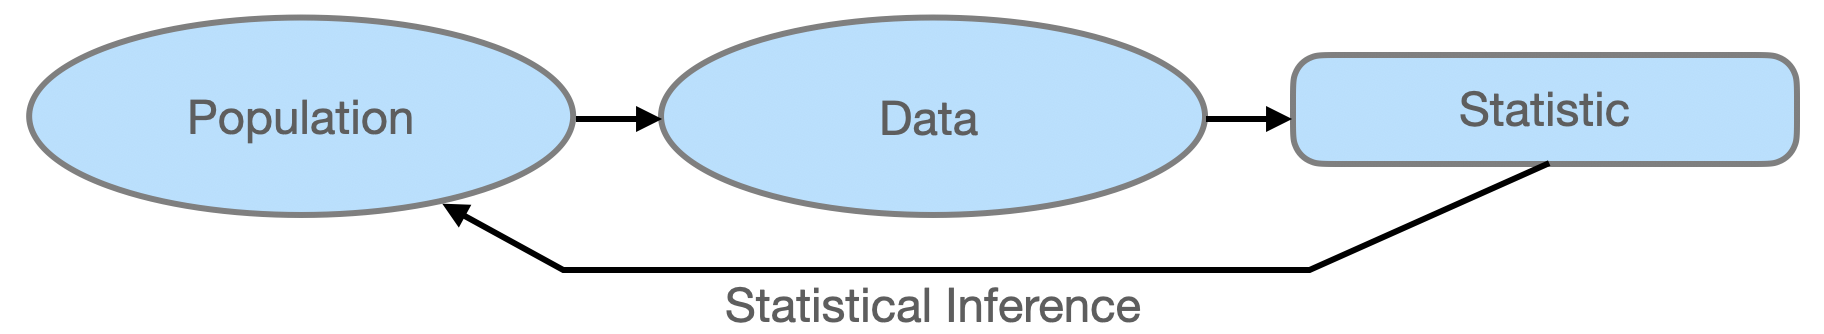
\includegraphics[width=0.75\linewidth,height=\textheight,keepaspectratio]{figures/inference_cycle.png}

}

\caption{\label{fig-cycle1}The canonical experiment-and-infer cycle. We
gather data sampled from an unknown population, and use statistics, or
functions of the data, to infer population properties.}

\end{figure}%

But, the reader says: the course is called \emph{Modern Probability and
Statistical Inference}. Where is probability in all of this? Probability
is the so-called ``language of statistics,'' and it provides the
mathematical framework upon which we can build statistical inference.
Remember how above we say that a population might be a mathematical
function indicating the relative rates of observing experimental
outcomes? Those relative rates \emph{are} probabilities (or at least
probability densities). Thus the structure of this chapter (and
``mathematical statistics'' courses as a whole): we discuss probability
first, and then use our newfound knowledge to show how the enterprise of
statistical inference works, both algorithmically and mathematically.

\section{Sample Spaces and the Axioms of
Probability}\label{sec-chap1sample}

What to take away from this section:

\begin{itemize}
\item
  The set of all experimental outcomes is a \emph{sample space} (denoted
  \(\Omega\)).
\item
  While in real-life analysis situations we rarely work with sample
  spaces and their contents directly\ldots{}

  \begin{itemize}
  \tightlist
  \item
    \ldots if the data-generating process is relatively simple (e.g., if
    we flip a coin two times and record the number of heads) \emph{and}
    if the experimental outcomes are discretely valued, there is value
    in directly examining sample space contents.
  \end{itemize}
\item
  The long-term frequency of the occurrence of an experiment outcome is
  its \emph{probability}.
\end{itemize}

Probability is the long-term frequency of the occurrence of an event.
For instance, what is the probability of flipping a coin and observing
heads? (Intuitively, this probability is 1/2, if the coin is fair.) Or:
what is the probability that a student finishes a particular test in
between 30 and 40 minutes? Etc.

To build up an understanding of probability, it is conventional to start
with the concept of a \emph{sample space}. A sample space is the set of
all possible outcomes of an ``experiment'' (or ``trial''), which is
simply some process that can, in theory, be repeated an infinite number
of times. (For instance, the flipping of a coin.) For instance, if our
experiment is to flip a single coin twice, the sample space would be \[
\Omega = \{HH,HT,TH,TT\} \,,
\] where \(H\) and \(T\) represent observing heads and tails,
respectively. (The Greek letter \(\Omega\) is a capital ``omega,'' or
``oh-MAY-gah.'') See Figure~\ref{fig-ss}.

\begin{figure}

\centering{

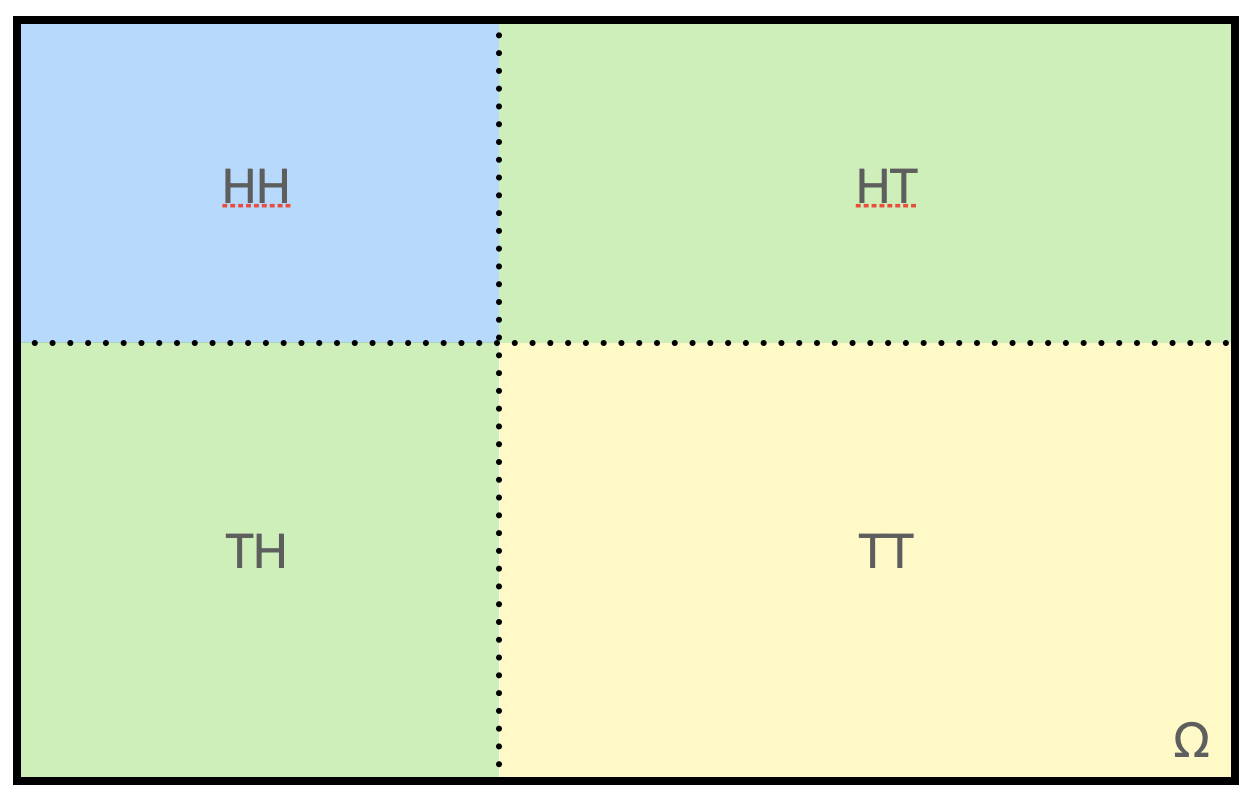
\includegraphics[width=0.6\linewidth,height=\textheight,keepaspectratio]{figures/samplespace.png}

}

\caption{\label{fig-ss}This is an example of a sample space \(\Omega\),
representing the experimental outcomes of flipping a single coin twice
and recording the observed side of the coin. For purposes of intuition,
it is common to associate the area shown for each outcome with that
outcome's probability of occurrence, so here we may view the coin as an
unfair one that favors tails.}

\end{figure}%

The members of the set \(\Omega\) are dubbed \emph{events} and they come
in two varieties:

\begin{enumerate}
\def\labelenumi{\arabic{enumi}.}
\tightlist
\item
  \emph{simple events}: specific experimental outcomes (e.g., \(HH\));
  any two simple events in \(\Omega\) are \emph{mutually exclusive}, or
  \emph{disjoint}, as they cannot be observed simultaneously in a single
  experiment.
\item
  \emph{compound events}: sets of two or more simple events (e.g.,
  \(\{HH,HT,TH\}\), which represents the set of outcomes where heads was
  observed at least once).
\end{enumerate}

As stated above, a sample space is a set of possible experimental
outcomes; thus we can apply set notation to, e.g., define specific
events as functions of others:

{\def\LTcaptype{none} % do not increment counter
\begin{longtable}[]{@{}lcc@{}}
\toprule\noalign{}
term & notation & intuitive terminology \\
\midrule\noalign{}
\endhead
\bottomrule\noalign{}
\endlastfoot
superset & \(A \supset B\) & ``encompasses'' \\
subset & \(A \subset B\) & ``within'' \\
union & \(A \cup B\) & ``or'' \\
intersection & \(A \cap B\) & ``and'' \\
complement & \(\bar{A}\) & ``not'' \\
\end{longtable}
}

We show examples of how we use set notation in the context of samples
spaces below.

Here are a few more things to keep in mind regarding sample spaces:

\begin{itemize}
\tightlist
\item
  The number of simple events in \(\Omega\) (i.e., the set's
  \emph{cardinality}) may be finite (as in the example above) or either
  countably or uncountably infinite (e.g., the set of all non-negative
  integers versus the set of real numbers). (For instance, the simple
  events in the experiment of repeating a task until one fails are
  \(\{F,SF,SSF,SSSF,\ldots\}\), where \(S\) denotes success and \(F\)
  denotes failure.)
\item
  The definition of a sample space can depend upon whether the order of
  outcomes matters. For instance, if the order of outcomes does not
  matter, we could rewrite our two-coin-flip sample space as
  \(\Omega = \{HH,HT,TT\}\) (or \(\{HH,TH,TT\}\)).
\item
  At no point thus far have we indicated the probability of observing
  any simple event. It is not the case in general that each experimental
  outcome is equally likely!
\end{itemize}

Regarding the last point above: while we may not know the probability of
observing any simple event, there are some things we can say about its
long-term relative frequency of occurrence:

\begin{enumerate}
\def\labelenumi{\arabic{enumi}.}
\tightlist
\item
  it must be \(\geq 0\) and \(\leq 1\);
\item
  the relative frequencies of all simple events in \(\Omega\) must sum
  to 1; and
\item
  the relative frequency of a compound event must equal the sum of the
  relative frequencies of its component simple events.
\end{enumerate}

These statements appear to be self-evident, and as thus may be dubbed
\emph{axiomatic}. (A mathematical axiom is a statement accepted without
proof.) In probability theory, these statements were recast as the
so-called Kolmogorov axioms, introduced by Kolmogorov (1933). Let \(A\)
denote an event within \(\Omega\) (i.e., \(A \subset S\)), either simple
or compound. A \emph{probability measure} on \(\Omega\) is a function
\(P\) from subsets of \(\Omega\) to \(\mathbb{R}^n\) that satisfies the
following:

\begin{enumerate}
\def\labelenumi{\arabic{enumi}.}
\tightlist
\item
  \(P(A) \in [0,1]\);
\item
  \(P(\Omega) = 1\); and
\item
  if \(\{B_1,\ldots,B_k\}\) is a set of mutually exclusive simple or
  compound events, then
  \(P(\bigcup_{i=1}^k B_i) = \sum_{i=1}^k P(B_i)\), where the symbol
  \(\bigcup\) refers to the \emph{union} of the set of events, i.e., the
  combination of all the events in the set into a single compound event.
\end{enumerate}

\subsection{Examples}\label{examples}

\subsubsection{Utilizing Set Notation}\label{utilizing-set-notation}

\begin{quote}
Let's suppose that we have in our hand one six-sided die, with faces
numbered 1 through 6. We roll it once, and observe the value on the
uppermost face. The sample space is \[
\Omega = \{1,2,3,4,5,6\} \,.
\] Let the event \(A\) be all odd-numbered outcomes, and let the event
\(B\) be all outcomes less than 4. Thus \(A = \{1,3,5\}\) and
\(B = \{1,2,3\}\).
\end{quote}

\begin{quote}
\begin{enumerate}
\def\labelenumi{\arabic{enumi}.}
\tightlist
\item
  What is \(\bar{A}\), the complement of \(A\)? It is the set of all
  outcomes not in \(A\), i.e., the set of all even-numbered faces:
  \(\bar{A} = \{2,4,6\}\).
\item
  What is \(A \cup B\), the union of \(A\) and \(B\)? It is the set of
  all outcomes observed in either \(A\) or \(B\), without double
  counting: \(A \cup B = \{1,2,3,5\}\) (and not
  \(A \cup B = \{1,1,2,3,3,5\}\)\ldots it is meaningless to write out
  the same experimental outcome twice).
\item
  What is \(A \cap B\), the intersection of \(A\) and \(B\)? It is the
  set of all outcomes observed in both \(A\) and \(B\), again without
  double counting: \(A \cap B = \{1,3\}\).
\end{enumerate}
\end{quote}

\begin{quote}
We note that we can combine unions, intersections, and complements in,
e.g., the \emph{distributive law}, \[
A \cap (B \cup C) = (A \cap B) \cup (A \cap C) \,,
\] the \emph{associative law}, \[
A \cup (B \cap C) = (A \cup B) \cap (A \cup C) \,,
\] and \emph{De Morgan's laws}, \[
\overline{A \cup B} = \bar{A} \cap \bar{B} ~~\mbox{and}~~ \overline{A \cap B} = \bar{A} \cup \bar{B} \,.
\]
\end{quote}

\subsubsection{Working With Contingency
Tables}\label{working-with-contingency-tables}

\begin{quote}
Let's assume that we are given the following information about two
events \(A\) and \(B\):
\end{quote}

{\def\LTcaptype{none} % do not increment counter
\begin{longtable}[]{@{}rcc@{}}
\toprule\noalign{}
\endhead
\bottomrule\noalign{}
\endlastfoot
& \(A\) & \(\bar{A}\) \\
\(B\) & 0.45 & 0.12 \\
\(\bar{B}\) & 0.21 & 0.22 \\
\end{longtable}
}

\begin{quote}
This is dubbed a \emph{contingency table} (or, more specifically here, a
two-by-two contigency table). The numbers in each cell represent
probabilities; for instance, \(P(A \cap B) = 0.45\). A contingency table
is appropriate to work with if the probabilities associated with each
event do not change from experiment to experiment.
\end{quote}

\begin{quote}
\begin{enumerate}
\def\labelenumi{\arabic{enumi}.}
\tightlist
\item
  What is \(P(A)\)? We can determine this by summing down the \(A\)
  column: \(P(A) = P[A \cap \Omega] = P[A \cap (B \cup \bar{B})] =
  P[(A \cap B) \cup (A \cap \bar{B})]\); since \(A \cap B\) and
  \(A \cap \bar{B}\) are disjoint, we can view the \(\cup\) as addition,
  and so
  \(P(A) = P(A \cap B) + P(A \cap \bar{B}) = 0.45 + 0.21 = 0.66\).
\item
  What is \(P(A \cup B)\)? Utilizing De Morgan's laws, this would be
  \(1 - P(\overline{A \cup B}) = 1 - P(\bar{A} \cap \bar{B}) = 1 - 0.22 = 0.78\).
\item
  What is the probability of observing \(A\) or \(B\), but not both?
  This would be \(P(A \cup B) - P(A \cap B)\), which is
  \(0.78 - 0.45 = 0.33\).
\end{enumerate}
\end{quote}

\begin{quote}
It is well worth taking the time to see how one could derive each of
these answers through visual inspection of the table. For instance,
\(P(A \cup B)\) is 1 minus the value in the cell at lower right, which
does not lie in the row for \(B\) or the column for \(A\).
\end{quote}

\section{Conditional Probability and the Independence of
Events}\label{sec-chap1conditional}

What to take away from this section:

\begin{itemize}
\item
  The probabilities of simple and compound events can be affected by
  invoking \emph{conditions}.
\item
  If invoking a condition does not change the probability of an event,
  then that event is said to be \emph{independent} of that conditioning
  event.
\end{itemize}

Intuitively, we can picture a sample space \(\Omega\) and two of its
constituent events as looking something like what we show in
Figure~\ref{fig-nondj}.

\begin{figure}

\centering{

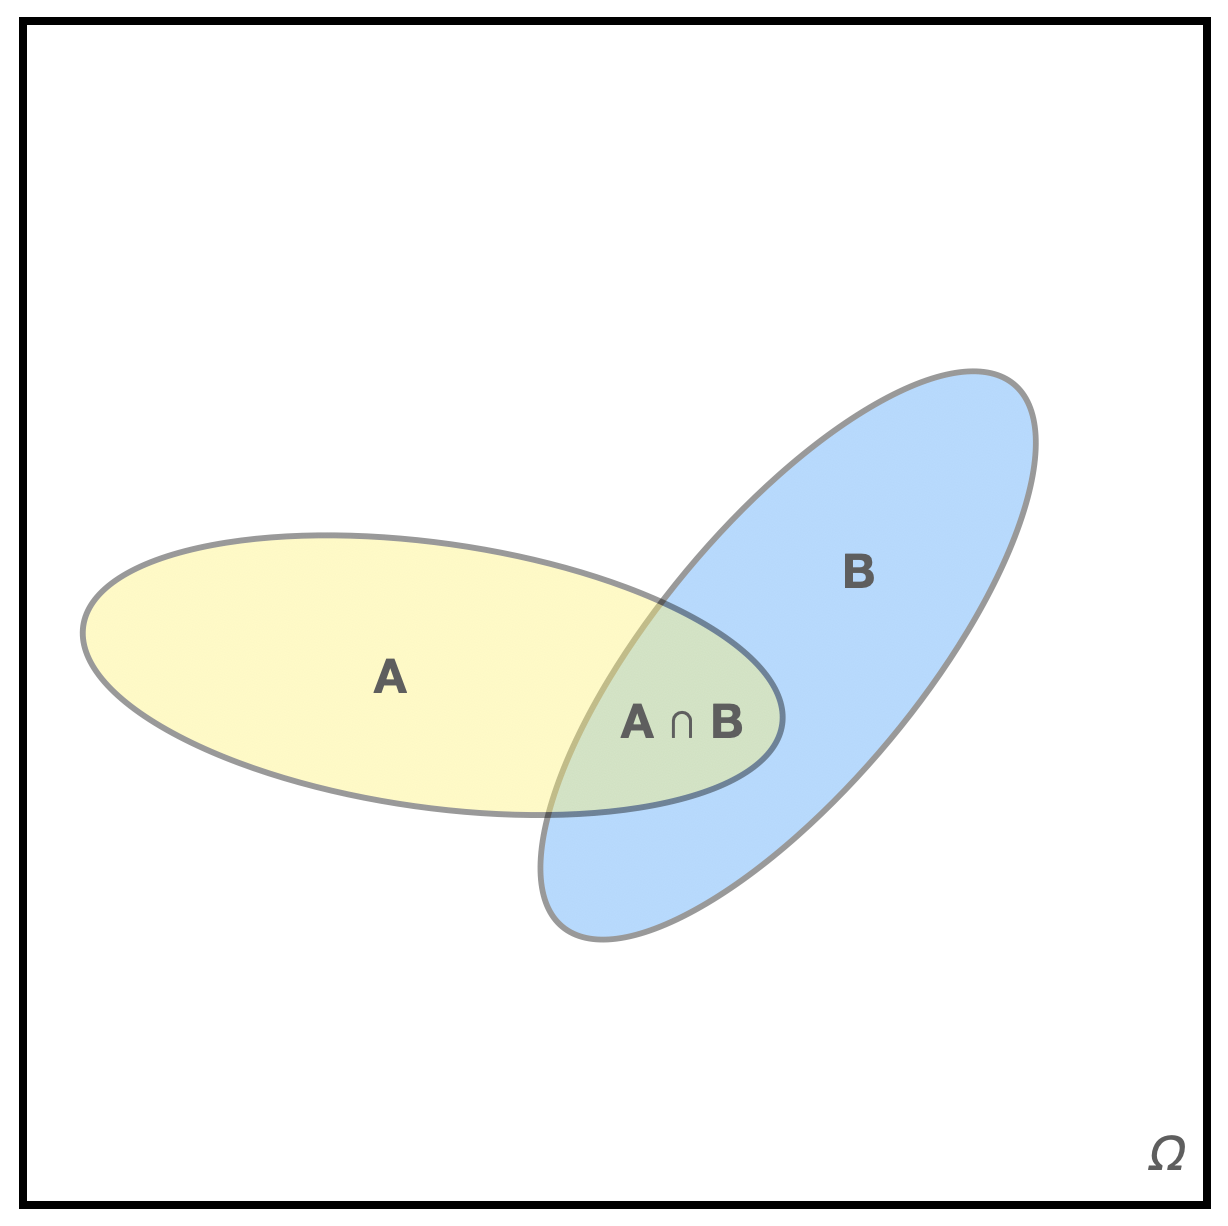
\includegraphics[width=0.5\linewidth,height=\textheight,keepaspectratio]{figures/conditional_event.png}

}

\caption{\label{fig-nondj}A sample space with non-disjoint events \(A\)
and \(B\).}

\end{figure}%

We can imagine that the geometric areas of each region represent
probability, with \(P(\Omega) = 1\) (given the second Kolmogorov axiom)
and \(P(A \cap B) > 0\) being the probability that both \(A\) and \(B\)
occur during an experiment. (Perhaps \(A\) is the event of speaking
French and \(B\) is the event of living is Brussels. The symbol \(\cap\)
denotes the intersection or overlap between two sets, whereas the
analogous symbol \(\cup\) represents the union of two sets.)

We can use this intuitive picture to illustrate the concept of
\emph{conditional probability}. A stated event probability, such as
\(P(A)\), is an \emph{unconditional probability}: its occurrence does
not depend on whether or not other events occur. To denote a conditional
probability, we add a vertical bar and place the conditions to the right
of it. For instance, \(P(A \vert B)\) denotes the probability that the
event \(A\) is observed, \emph{given} that the event \(B\) is observed.
(Note that there is no implied causality: it is not necessarily the case
that \(B\) occurring is ``causing'' changes to the probability that
\(A\) will occur.) To illustrate why \(P(A)\) may not equal
\(P(A \vert B)\), we first point out that \(P(A) = P(A \vert \Omega)\),
which we may think of as ``the probability of observing the event \(A\)
if we observe the event \(\Omega\),'' which is the ratio of geometric
areas of \(A \cap \Omega\) and \(\Omega\): \[
P(A) = P(A \vert \Omega) = \frac{P(A \cap \Omega)}{P(\Omega)} \,.
\] When we condition on the event \(B\), we are reducing the set of
possible outcomes from the full sample space \(\Omega\) to \(B\), i.e.,
we are replacing \(\Omega\) in the expression above with \(B\): \[
P(A \vert B) = \frac{P(A \cap B)}{P(B)} \,,
\]

In the context of our intuitive picture, we are changing the one shown
above to the one we show in Figure~\ref{fig-sscond}.

\begin{figure}

\centering{

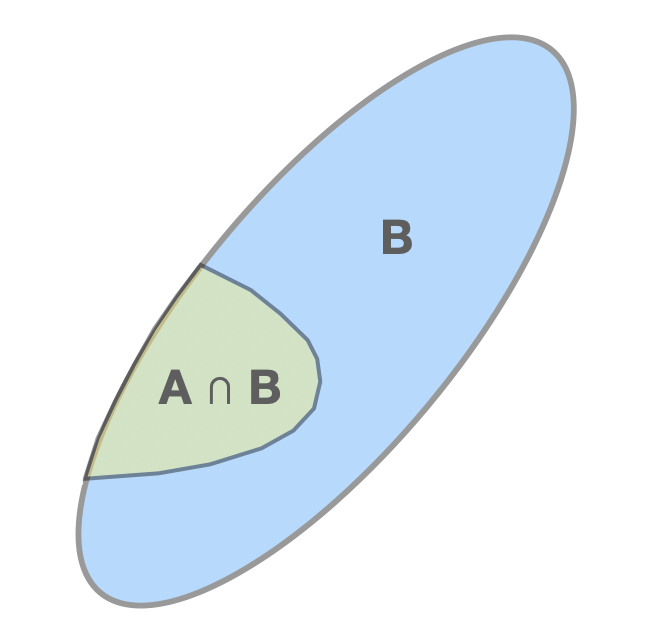
\includegraphics[width=0.4\linewidth,height=\textheight,keepaspectratio]{figures/conditional_event_ii.png}

}

\caption{\label{fig-sscond}The new sample space that arises when we
condition on the event \(B\).}

\end{figure}%

\(B\) thus defines a new ``sample space.''

Two events \(A\) and \(B\) are independent if the probability of
observing one does not depend on the probability of observing the other.
The intuitive picture many have of independence is the one shown in
Figure~\ref{fig-dj}.

\begin{figure}

\centering{

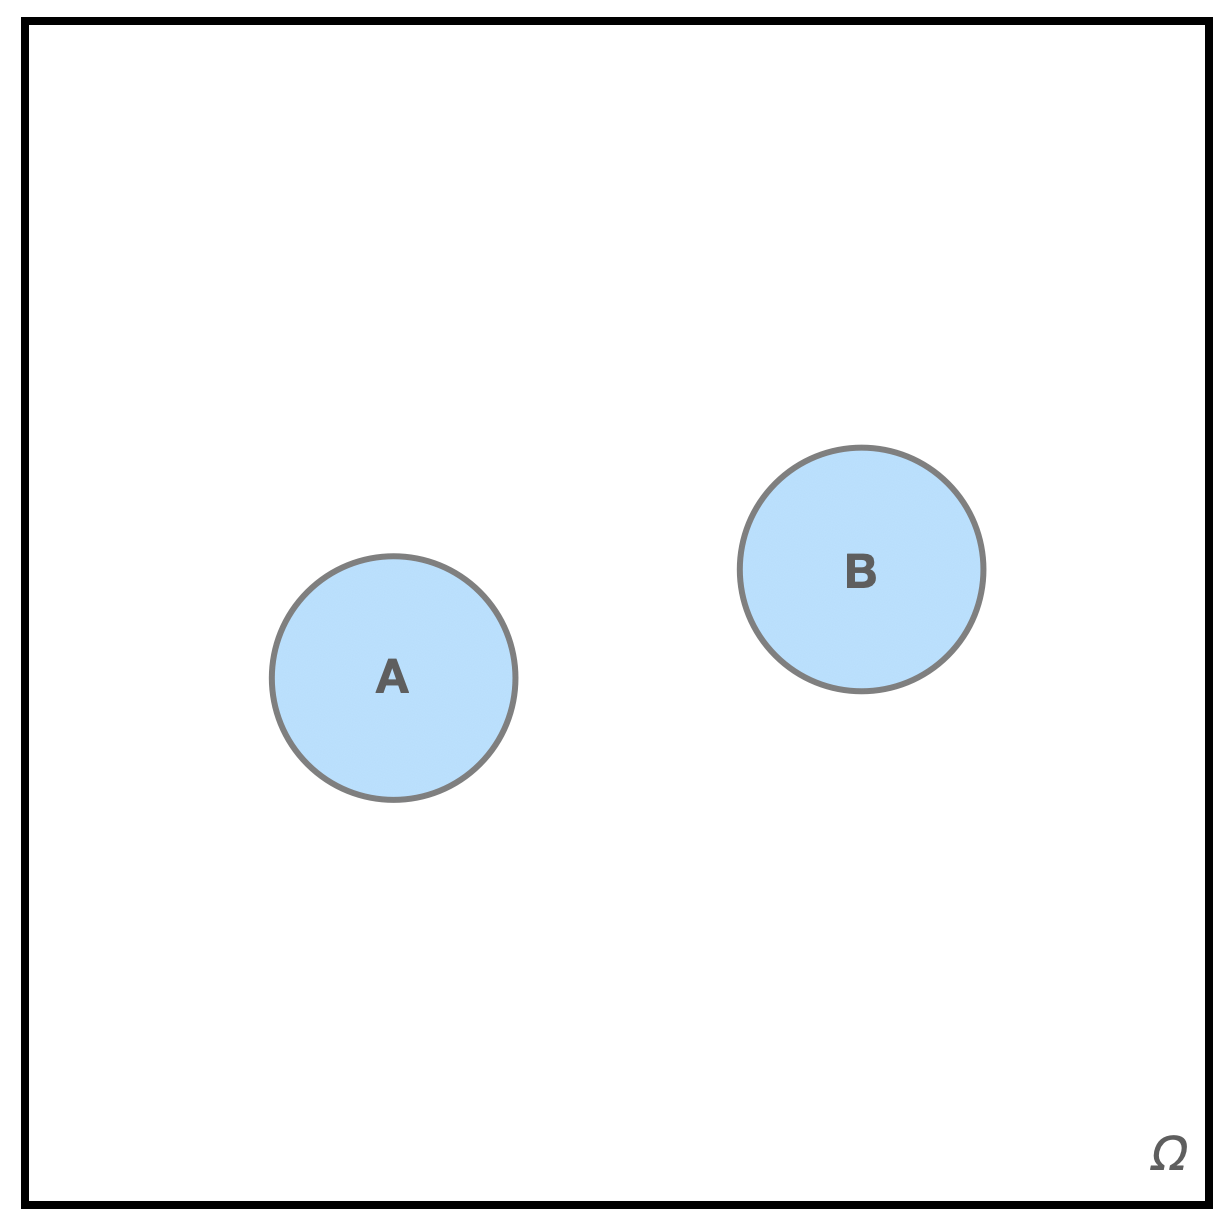
\includegraphics[width=0.5\linewidth,height=\textheight,keepaspectratio]{figures/disjoint_event.png}

}

\caption{\label{fig-dj}To many, \(A\) and \(B\) appear to be independent
events\ldots but they are simply disjoint.}

\end{figure}%

The events \(A\) and \(B\) do not overlap\ldots hence they are
independent events, right? No: they are simply disjoint events. Also,
with reflection, we realize that if, e.g., the event \(A\) is observed
in a given experiment, then we know that \(B\) \emph{cannot be
observed}. So these events are very much dependent! Figure~\ref{fig-ind}
shows how we can actually represent \(A\) and \(B\) as independent
events. In this figure, the ratio of the geometric area associated with
the event \(A\) to the geometric area of \(\Omega\) is equal to the
ratio of the areas of \(A \cap B\) and \(B\). Thus we can write that \[
P(A) = P(A \vert \Omega) = \frac{P(A \cap \Omega)}{P(\Omega)} = \frac{P(A \cap B)}{P(B)} = P(A \vert B) \,.
\] The probability of observing the event \(A\) is unchanged if the
event \(B\) occurs: \(A\) and \(B\) are independent events.

\begin{figure}

\centering{

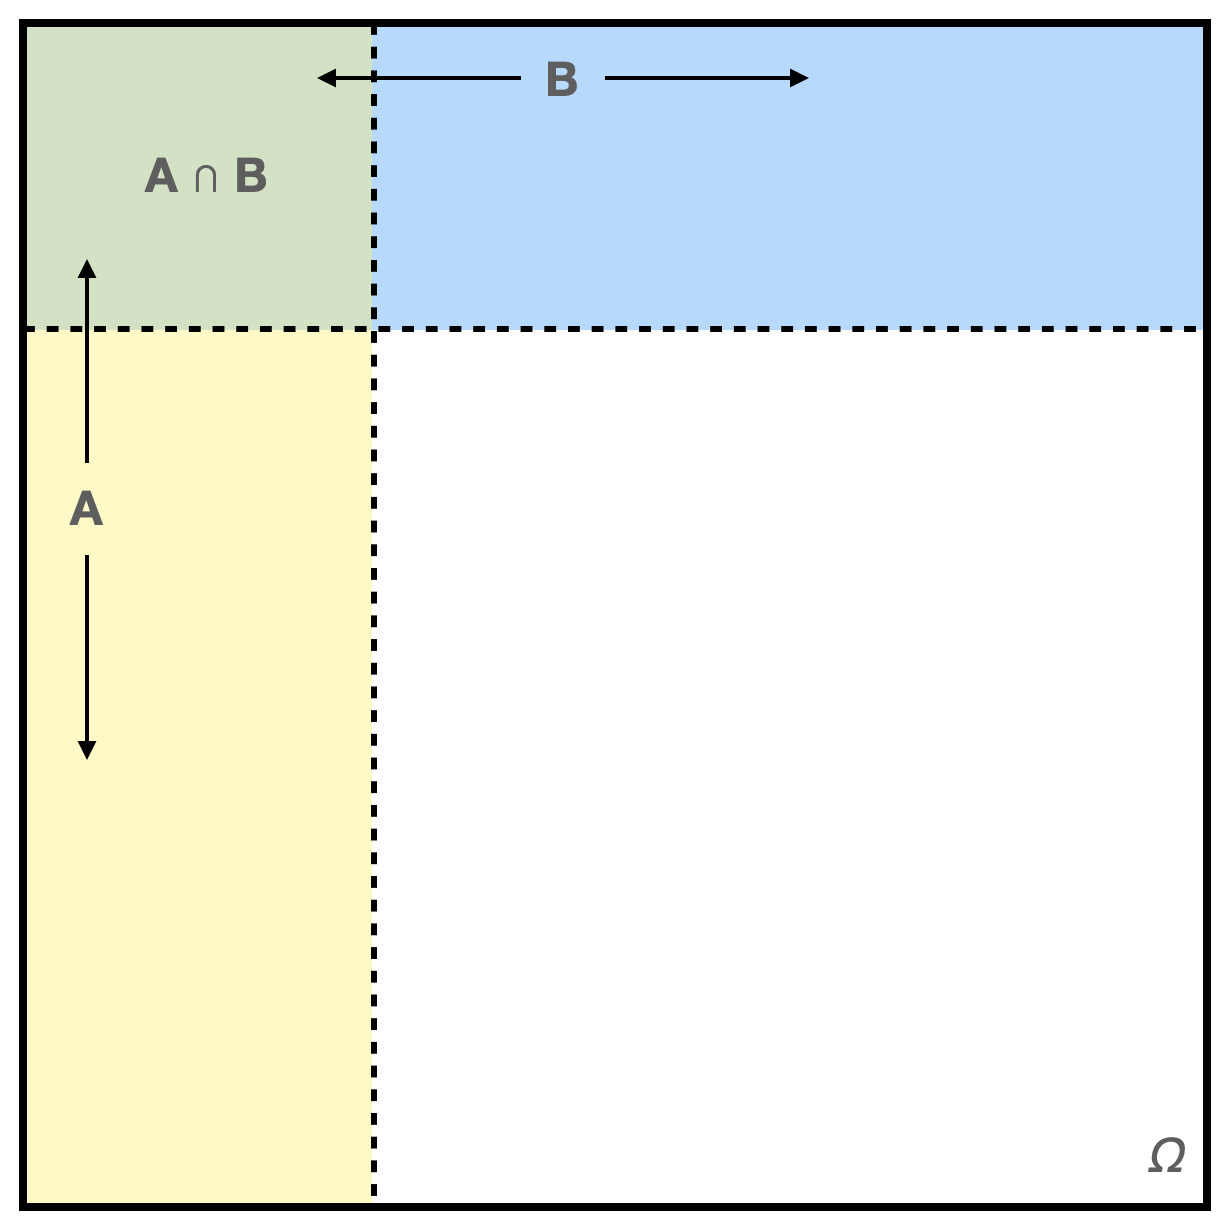
\includegraphics[width=0.5\linewidth,height=\textheight,keepaspectratio]{figures/independent_event.png}

}

\caption{\label{fig-ind}\(A\) and \(B\) are independent events.}

\end{figure}%

\subsection{Examples}\label{examples-1}

\subsubsection{Visualizing Conditional Probabilities: Contingency
Tables}\label{visualizing-conditional-probabilities-contingency-tables}

\begin{quote}
Let's recall the two-by-two contingency table we defined in the previous
section, but with some additional information added:
\end{quote}

{\def\LTcaptype{none} % do not increment counter
\begin{longtable}[]{@{}rccc@{}}
\toprule\noalign{}
\endhead
\bottomrule\noalign{}
\endlastfoot
& \(A\) & \(\bar{A}\) & \\
\(B\) & 0.45 & 0.12 & 0.57 \\
\(\bar{B}\) & 0.21 & 0.22 & 0.43 \\
& 0.67 & 0.33 & \\
\end{longtable}
}

\begin{quote}
The numbers in the so-called ``margins'' are the row and column sums,
so, for instance, \(P(A) = 0.67\). This information is useful to have
when computing conditional probabilities. In analogy with what was
stated above about imposing conditions and what that does to the sample
space, here we can say that imposing a condition will restrict us to a
given row or a given column. For instance, what is
\(P(\bar{A} \vert B)\)? The condition restricts us to the top row, and
within that row, the probability of observing the event \(\bar{A}\) is
0.12/0.57 = 0.21. So
\(P(\bar{A} \vert B) = P(\bar{A} \cap B) / P(B) = 0.21\).
\end{quote}

\begin{quote}
Now, are \(A\) and \(B\) independent events? The easy way to visually
infer this given a two-by-two table is to see if the rows (or columns)
are multiples of each other\ldots meaning, here, is there a number \(a\)
such that \(0.45 = 0.21 a\) \emph{and} \(0.12 = 0.22 a\)? The answer
here is no\ldots so the events \(A\) and \(B\) are dependent events.
(The conventional, yet longer way to determine independence is to see
if, e.g., \(P(A \vert B) = P(A)\); if so, \(A\) and \(B\) are
independent.)
\end{quote}

\subsubsection{Conditional Independence}\label{conditional-independence}

\begin{quote}
If \(A\) and \(B\) are independent events, is it automatically the case
that the events \(A \vert C\) and \(B \vert C\) are also independent
events?
\end{quote}

\begin{quote}
Recall the figure above that shows how independent events appear in a
Venn diagram. Recall also that if we impose a condition \(C\), we
effectively change the sample space from \(\Omega\) to \(C\). Imagine
\(C\) as an arbitrarily shaped region superimposed on the last figure,
so that now we have a situation like the one in
Figure~\ref{fig-condind}.
\end{quote}

\begin{figure}

\centering{

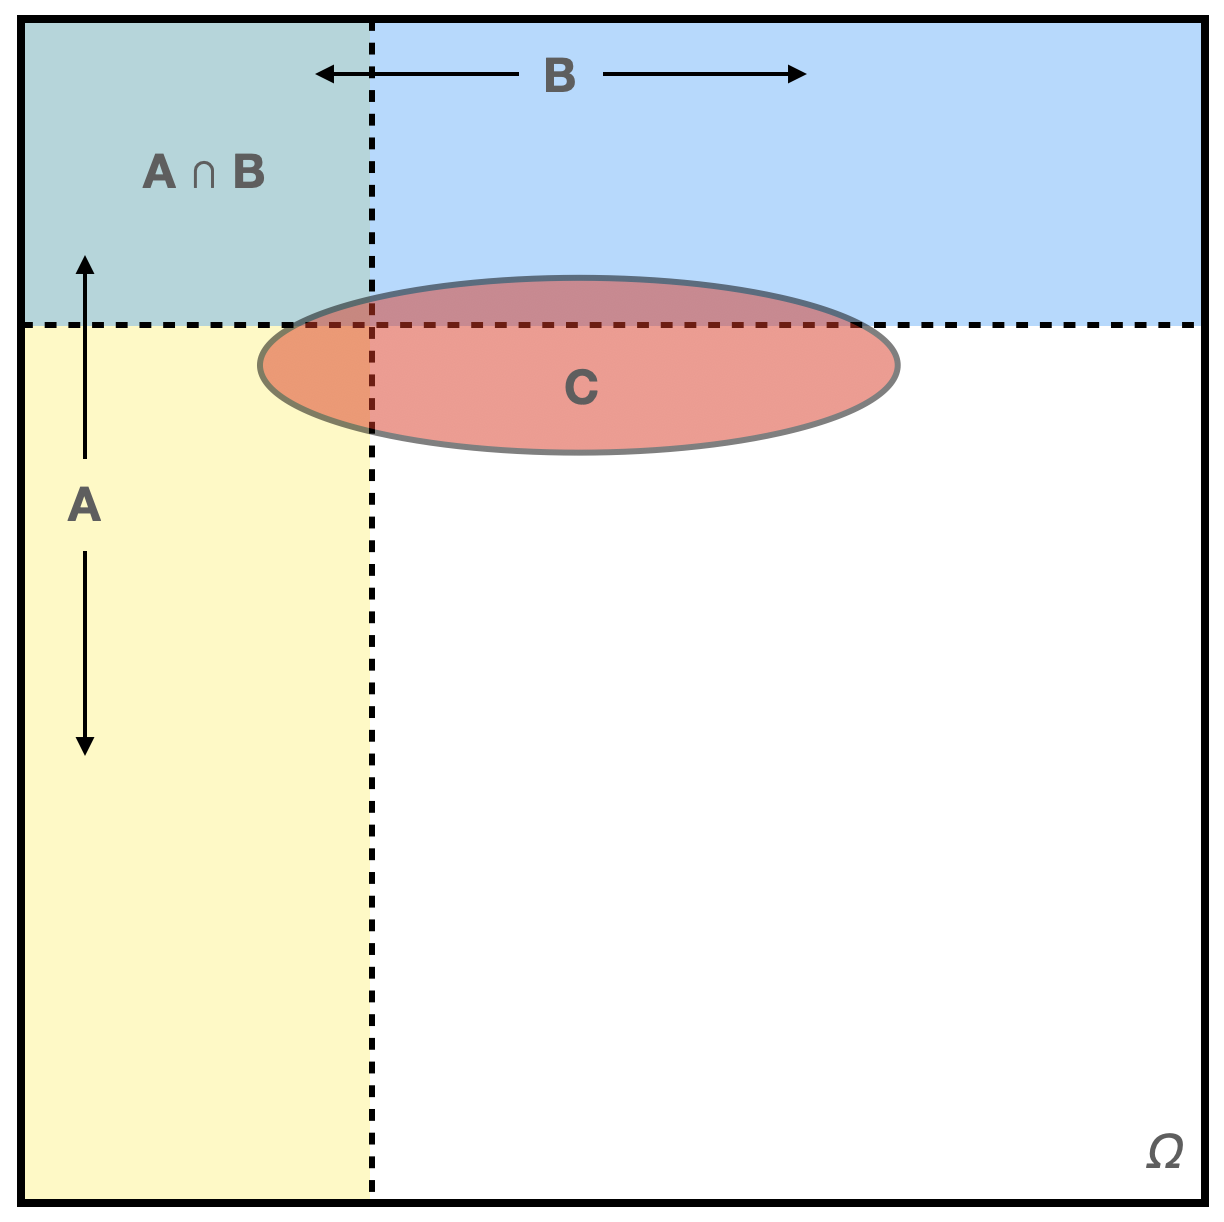
\includegraphics[width=0.5\linewidth,height=\textheight,keepaspectratio]{figures/cond_ind_event.png}

}

\caption{\label{fig-condind}\(A\) and \(B\) are not necessarily
independent events, given \(C\).}

\end{figure}%

\begin{quote}
The events \(A\) and \(B\) are conditionally independent given \(C\) if
\(P(C) > 0\) and \(P(A \cap B \vert C) = P(A \vert C) P(B \vert C)\). As
we can see in Figure~\ref{fig-condind}, \(C\) can be made to overlap
\(B\), \(A\), and \(A \cap B\) in any number of ways such that
\(P(A \cap B \vert C) \neq P(A \vert C) P(B \vert C)\)\ldots so it is
\emph{not} the case that if \(A\) and \(B\) are independent,
\(A \vert C\) and \(B \vert C\) are always independent. (If \(C\) had a
rectangular shape with a horizontal base and top and vertical sides,
conditional independence \emph{would} hold. Think through why this would
be true\ldots)
\end{quote}

\section{Further Laws of Probability}\label{sec-chap1further}

What to take away from this section:

\begin{itemize}
\item
  The four core tools for solving conditional probability problems
  are\ldots{}

  \begin{itemize}
  \item
    the \emph{multiplicative law};
  \item
    the \emph{additive law};
  \item
    the \emph{law of total probability}; and
  \item
    \emph{Bayes' rule}.
  \end{itemize}
\end{itemize}

Now that we have learned about the concepts of conditional probabilities
and independence, we can write down some useful laws that one can use to
solve an array of probability-based problems.

\begin{itemize}
\tightlist
\item
  \emph{Multiplicative Law}. This follows simply from rearranging the
  definition of conditional probability: \[
  P(A \cap B) = P(A) P(B \vert A) = P(B) P(A \vert B)
  \] We can generalize this law given an arbitrary number of events
  \(k\): \begin{align*}
  P(A_1 \cap A_2 \cap \cdots \cap A_k) &= P(A_1 \vert A_2 \cap \cdots \cap A_k) P(A_2 \cap \cdots \cap A_k) = \cdots \\
  &= P(A_k) \prod_{i=1}^{k-1} P(A_i \vert A_{i+1} \cap \cdots \cap A_k) \,,
  \end{align*} where \(\prod\) is the product symbol, the multiplicative
  analogue to the summation symbol \(\sum\).
\item
  \emph{Additive Law}. The probability of the union of two events \(A\)
  and \(B\) is \[
  P(A \cup B) = P(A) + P(B) - P(A \cap B) \,.
  \] If the events \(A\) and \(B\) are not disjoint, then if we add
  their probabilities, we count the probability of \(A \cap B\)
  twice\ldots hence the subtracted term.
\item
  \emph{Law of Total Probability (LoTP)}. Assume that we partition the
  sample space \(\Omega\) into \(k\) disjoint (simple or compound)
  events \(\{B_1,\ldots,B_k\}\), all of which have non-zero probability
  of occurring. Then, given any event \(A\), we can write \[
  P(A) = \sum_{i=1}^k P(A \vert B_i) P(B_i) \,.
  \]
\item
  \emph{Bayes' Rule}. Continue to assume that the sample space is
  partitioned into the events \(\{B_1,\ldots,B_k\}\). The conditional
  probability of each of these events, given that \(A\) occurs, is \[
  P(B_i \vert A) = \frac{P(A \vert B_i) P(B_i)}{\sum_{j=1}^k P(A \vert B_j)P(B_j)} = \frac{P(A \vert B_i)P(B_i)}{P(A)} \,.
  \]
\end{itemize}

\subsection{Examples}\label{examples-2}

\subsubsection{The Additive Law for Independent
Events}\label{the-additive-law-for-independent-events}

\begin{quote}
Let's assume that for a given experiment, we can define the independent
events \(A\) and \(B\), with \(P(A) = 0.6\) and \(P(B) = 0.4\). What is
\(P(A \cup B)\)?
\end{quote}

\begin{quote}
In general, when solving probability problems, we look at all the rules
and relationships at our disposal and see which one (or more!) contains
the probabilities we know and the one we don't know, and we use that
rule or relationship to derive the solution. Here, there is nothing that
directly relates \(A\) and \(B\) to \(A \cup B\)\ldots the events may
overlap when represented on a Venn diagram, and we don't know by how
much. Except\ldots we are given the word ``independent.'' That allows us
to say that \(P(A \cap B) = P(A)P(B)\)\ldots and now we know that the
additive law is in play: \begin{align*}
P(A \cup B) &= P(A) + P(B) - P(A \cap B) \\
&= P(A) + P(B) - P(A \vert B)P(B) \\
&= P(A) + P(B) - P(A)P(B) = 0.6 + 0.4 - 0.6 \cdot 0.4 = 0.76 \,.
\end{align*} Is this the only way to solve the problem? No\ldots we know
from De Morgan's laws that
\(\overline{A \cup B} = \bar{A} \cap \bar{B}\), and thus \begin{align*}
P(A \cup B) &= 1 - P(\overline{A \cup B}) = 1 - P(\bar{A} \cap \bar{B}) = 1 - P(\bar{A} \vert \bar{B})P(\bar{B}) \\
&= 1 - P(\bar{A})P(\bar{B}) = 1 - (1-0.6)(1-0.4) = 0.76 \,.
\end{align*} There is no ``right'' way to solve a probability
problem\ldots just correct ones.
\end{quote}

\subsubsection{The Monty Hall Problem}\label{the-monty-hall-problem}

\begin{quote}
\emph{Let's Make a Deal} is a game show that has appeared on television
at various times since 1963. During one part of the show, contestants
are brought on stage and presented with three closed doors; behind one
is an expensize prize (say, a car or an around-the-world cruise), and
behind the other two are inexpensive prizes (like a year's supply of
Turtle Wax\textregistered). The contestant is asked to pick a door (say,
Door \#1), at which point the show's host will open another door (say,
Door \#3) and show the inexpensive prize behind that door (thereby
taking that door out of play). The contestant is then asked if they want
to stick with the door they've chosen (here, Door \#1), or switch their
choice to the other unopened door (here, Door \#2). What should we
advise the constestant to do?
\end{quote}

\begin{quote}
The original, and most famous, host of \emph{Let's Make a Deal} was
Monty Hall. Hence: the Monty Hall Problem. (Note that the problem is
often stated such that there is a car being behind one door and goats
behind the other two. The author is old enough to have seen the show in
its heyday and he recalls seeing no goats. Or maybe they made no
impression at the time\ldots)
\end{quote}

\begin{quote}
Assume, without loss of generality, that Door \#1 is chosen. Then, let
\end{quote}

\begin{quote}
\begin{itemize}
\tightlist
\item
  \(O_i\) = ``Monty Hall opens Door \#\(i\)''
\item
  \(C_i\) = ``The car is behind Door \#\(i\)''
\end{itemize}
\end{quote}

\begin{quote}
and assume that \(P(C_i) = 1/3\) for all \(i\). (The car could have been
placed behind any door before the show was filmed.) The sample space of
experimental outcomes is \[
\Omega = \{ O_2 \cap C_1 , O_2 \cap C_3 , O_3 \cap C_1 , O_3 \cap C_2\} \,.
\] Why not \(O_2 \cap C_2\) and \(O_3 \cap C_3\)? Monty is not stupid:
he won't open the door the car is behind. (He knows where it is!)
\end{quote}

\begin{quote}
Let's assume, again without any loss of generality, that Monty opens
Door \#3. The probability we want to compute is \(P(C_2 \vert O_3)\):
what is the probability that the car is actually behind Door \#2? (Note
that this is \(1 - P(C_1 \vert O_3)\)\ldots again,
\(P(C_3 \vert O_3) = 0\), as Monty is not stupid.) Is this probability
1/2? We utilize Bayes' rule and the LoTP to write \begin{align*}
P(C_2 \vert O_3) &= \frac{P(O_3 \vert C_2) P(C_2)}{P(O_3)}\\
&= \frac{P(O_3 \vert C_2) P(C_2)}{P(O_3 \vert C_2) P(C_2) + P(O_3 \vert C_1) P(C_1)}\\
&= \frac{P(O_3 \vert C_2)}{P(O_3 \vert C_2) + P(O_3 \vert C_1)}\,.
\end{align*} What do we know?
\end{quote}

\begin{quote}
\begin{itemize}
\tightlist
\item
  \(P(O_3 \vert C_2) = 1\): if the car is behind Door \#2, Monty has to
  open Door \#3
\item
  \(P(O_3 \vert C_1) = 1/2\): Monty can open either Door \#2 or \#3 if
  the car is behind Door \#1
\end{itemize}
\end{quote}

\begin{quote}
Hence \[
P(C_2 \vert O_3) = \frac{1}{1 + 1/2} = \frac{2}{3} \,.
\] \emph{We should advise the contestant to open Door \#2!}
\end{quote}

\begin{quote}
Confused? Think about the solution this way: the contestant has a
one-third chance of correctly picking the door the car is behind, and a
two-thirds chance of being wrong. Opening one of the other doors (while
knowing there is no car behind it) doesn't change these conditions at
all: the contestant still has a one-third chance of having initially
picked the correct door. Thus the contestant should change their pick to
the other unopened door.
\end{quote}

\subsubsection{Visualizing Conditional Probabilities: Tree
Diagrams}\label{visualizing-conditional-probabilities-tree-diagrams}

\begin{quote}
In the previous sections, we show how one can use contingency tables to
aid the visualization of probabilities (and to solve for probabilities
of simple and/or compound events). Here we show another, somewhat more
general probability visualizer: the \emph{tree diagram}. Why ``somewhat
more general''? First, a tree in a tree diagram can have arbitrary
depth: if we have events \(A\), \(B\), and \(C\), the table would be
three-dimensional, with the axes representing the experimental outcome
in terms of \(A\) and \(\bar{A}\), \(B\) and \(\bar{B}\), and \(C\) and
\(\bar{C}\). A table is not an optimal means to represent probabilities.
And second, a tree is arguably a more natural means to represent
probabilities when an experiment represents sequential outcomes,
particularly when we sample \emph{without} replacement.
\end{quote}

\begin{quote}
Let's elaborate on that second point. Let's say we have a drawer with
five socks, three of which are red and two of which are blue. We plan to
draw three socks in succession from the drawer without placing the socks
back into the drawer, but we will stop early if we draw two socks of the
same color on the first two draws. What is the probability that our
final sample contains two blue socks?
\end{quote}

\begin{quote}
We can write out the following: if \(B_i\) and \(R_i\) are the
probabilities of drawing a blue and red sock from the drawer when taking
out the \(i^{\mathrm{th}}\) sock, then \(P(B_1) = 2/5\) and
\(P(R_1) = 3/5\)\ldots and \(P(B_2 \vert B_1) = 1/4\) because there is
one less blue sock in the drawer, and\ldots{} Actually, this gets tiring
quickly. Let's use a tree diagram instead.
\end{quote}

\begin{figure}

\centering{

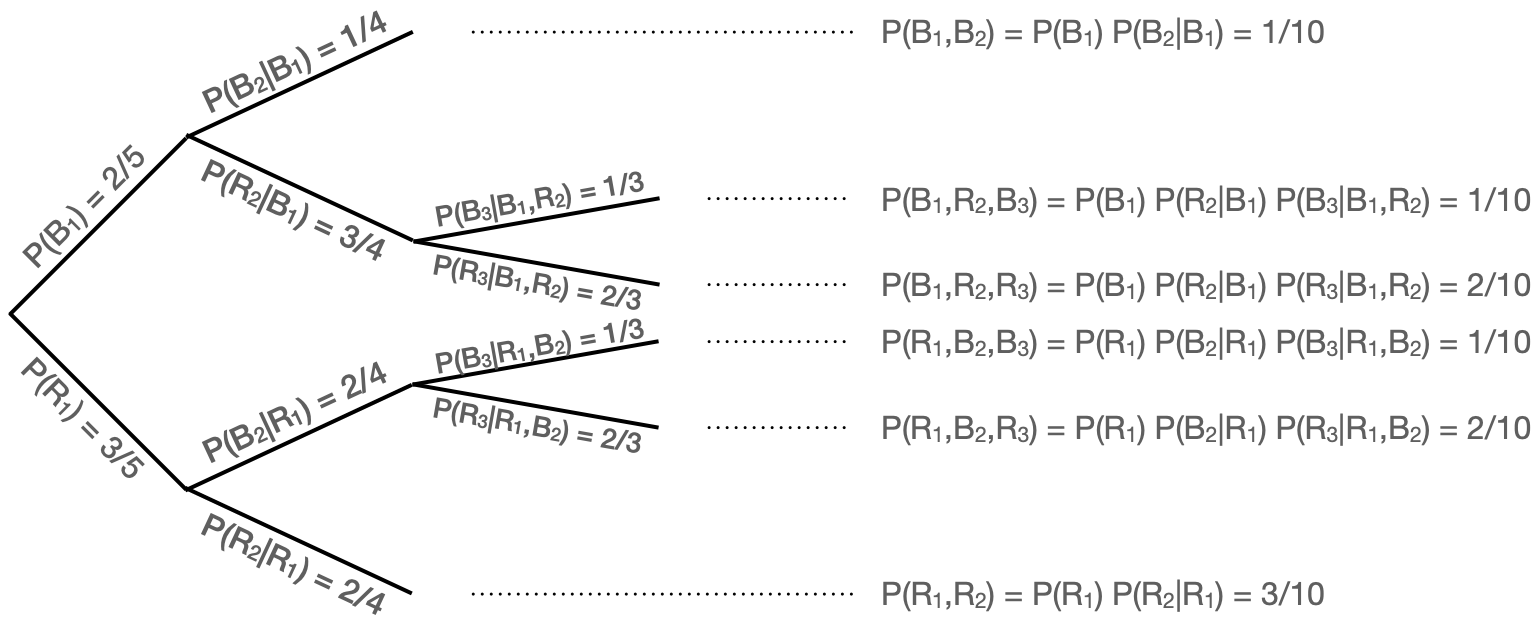
\includegraphics[width=0.8\linewidth,height=\textheight,keepaspectratio]{figures/decision_tree.png}

}

\caption{\label{fig-tree}An example of visualizing probabilities using a
decision tree.}

\end{figure}%

\begin{quote}
In Figure~\ref{fig-tree}, we show the tree diagram for this problem. We
note some aspects of this diagram:
\end{quote}

\begin{quote}
\begin{enumerate}
\def\labelenumi{\arabic{enumi}.}
\tightlist
\item
  the tree can be truncated along some branches (here, that's because we
  stop removing socks from the drawer if we remove two of the same color
  in the first two draws);
\item
  at any branching point, the (conditional) probabilities of going down
  each branch sum to one; and
\item
  the probability of ending up at a particular leaf (where the leaves
  collectively represent the simple events of the experiment) is the
  product of all the branch probabilities leading to that leaf.
\end{enumerate}
\end{quote}

\begin{quote}
So, now, what is the probability of drawing two blue socks in this
experiment? To find that, we determine which leaves are associated with
drawing two blue socks; from the top, that would be leaves 1, 2, and 4,
with probabilities 1/10, 1/10, and 1/10. Because simple events are
disjoint by definition, the probability of the compound event is simply
the sum of the probabilities of the simple events, which here is 3/10.
In any given replication of this experiment, we have a 30\% chance of
ending up with two blue socks.
\end{quote}

\section{Random Variables}\label{sec-chap1random}

What to take away from this section:

\begin{itemize}
\item
  Working directly with sample space contents only works in limited
  situations (such as having a small number of discrete experiment
  outcomes).
\item
  We can shift our focus from sample spaces to, e.g., the real-number
  line by encapsulating the contents of the former as \emph{random
  variables}.
\item
  Random variables themselves do not contain information about the
  probability of the events they represent\ldots for that, we will need
  to pair random variables with \emph{probability distributions}, as we
  will show in the next section.
\end{itemize}

Let's say that we perform an experiment in which we flip a fair coin
three times. Let \(H\) denote observing heads, and \(T\) tails. The
sample space of outcomes \(\Omega\) is \[
\{ HHH,HHT,HTH,THH,HTT,THT,TTH,TTT\}
\] and each outcome is observed with probability 1/8. What is the
probability of observing exactly one tail? We can determine this by
laboriously generating a table of probabilities, like so: \begin{align*}
P(\mbox{"no tails"}) &= P(HHH) = 1/8 \\
P(\mbox{"one tail"}) &= P(HHT \cup HTH \cup THH) = 3/8 \\
P(\mbox{"two tails"}) &= P(HTT \cup THT \cup TTH) = 3/8 \\
P(\mbox{"three tails"}) &= P(TTT) = 1/8 \,.
\end{align*} One can easily imagine how, if we were to flip a coin 50
times, or 500 times, the generation of tables would be onerous. A better
way to portray the information in a sample space is to use a
\emph{random variable}. In probability theory, a random variable \(X\)
is a measurable function mapping from a set of outcomes (here,
\(\Omega\)) to a measurable space (here, \(\mathbb{R}^n\), where
\(\mathbb{R}^1 = \mathbb{R}\) is the real-number line). (See
Figure~\ref{fig-rv}.) While \(X\) is a function, it is natural in an
undergraduate context to think of it as a variable whose value is an
experimental outcome. For instance, if we define \(X\) as being ``the
number of tails observed in three flips of a fair coin,'' then
\(P(X=1) = 3/8\). (Below, we will complete our transition away from
laboriously built probability tables by introducing mathematical
functions\(-\)\emph{probability mass functions} or \emph{probability
density functions} associated with \emph{distributions}\(-\)that allow
us to compute probabilities more generally, as a function of an
arbitrary observed value \(X=x\) or a range of observed values
\(X \in [a,b]\).)

\begin{figure}

\centering{

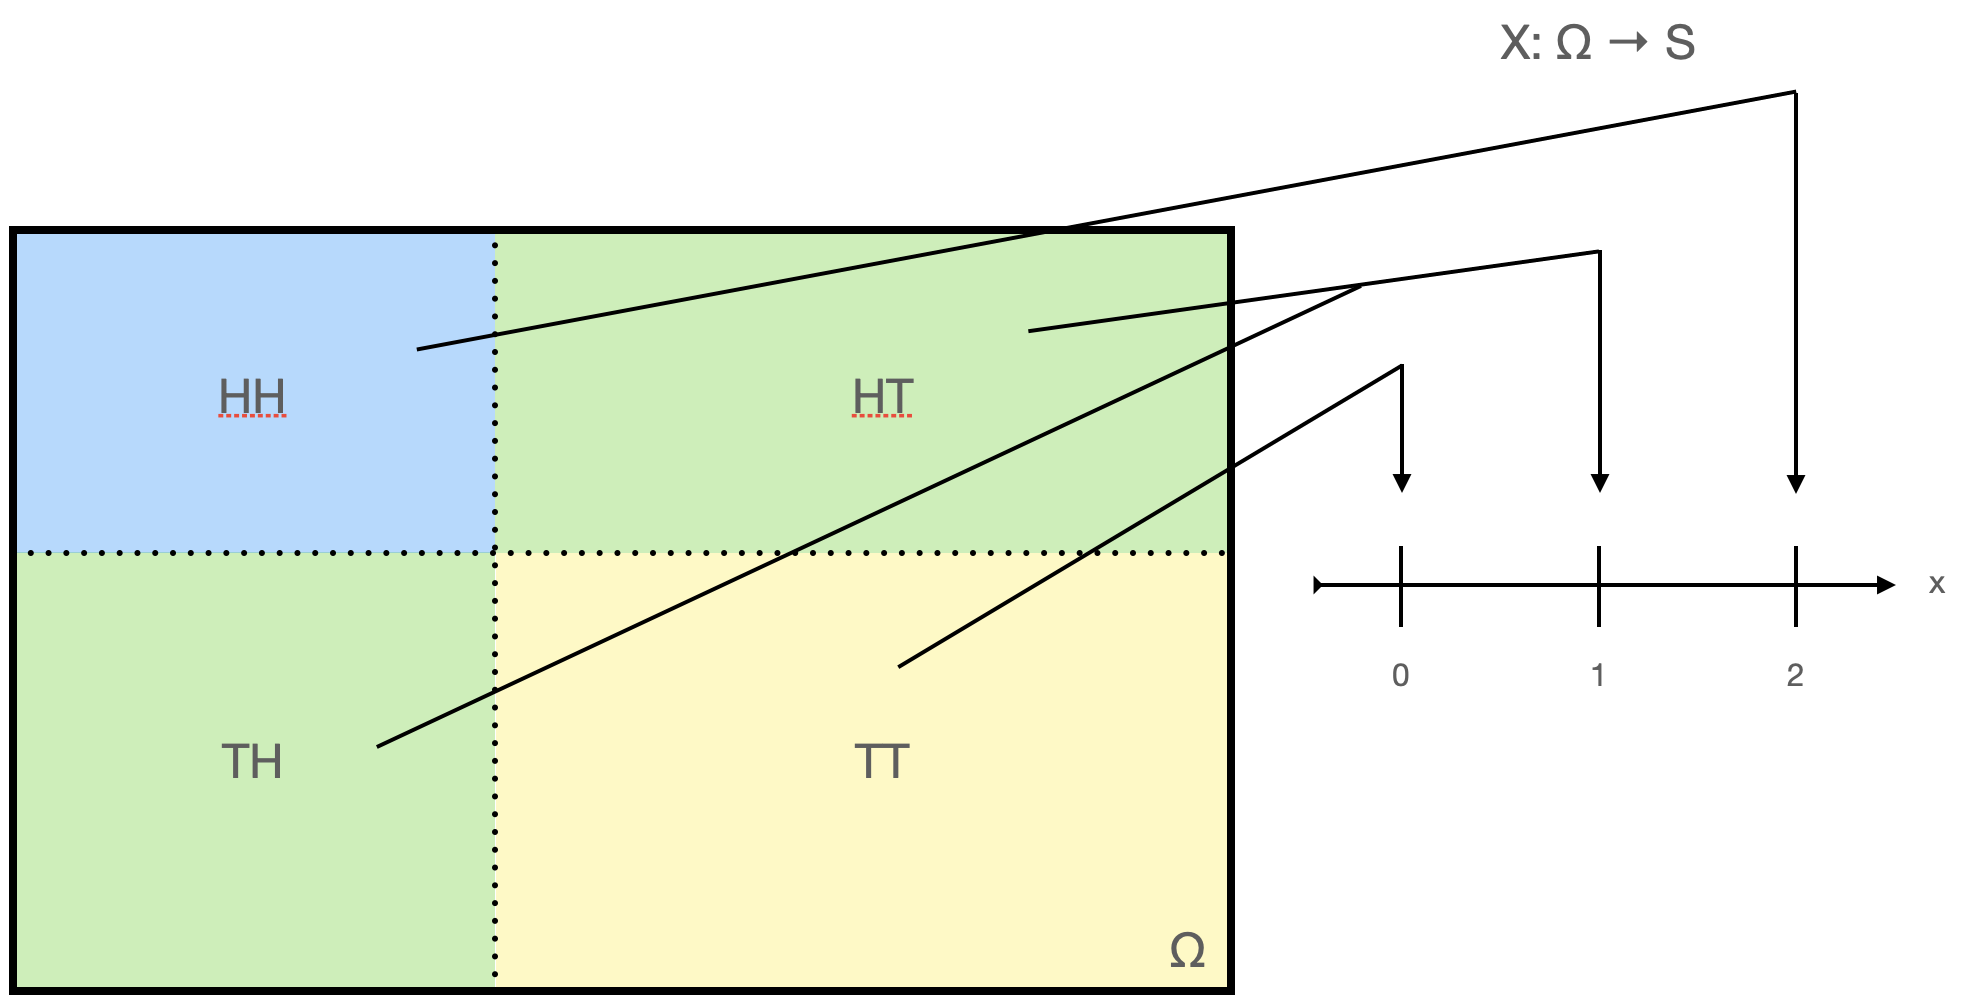
\includegraphics[width=0.75\linewidth,height=\textheight,keepaspectratio]{figures/measurablespace.png}

}

\caption{\label{fig-rv}A random variable is a function that maps events
in \(\Omega\) to the real-number line \(\mathbb{R}\).}

\end{figure}%

There are a few initial things to note about random variables. First,
they are conventionally denoted with capital Latin letters (e.g., \(X\),
\(Y\), \(Z\)). Second, note the words ``if we define'' above. There is
no unique random variable associated with a sample space. In addition to
\(X\), we could just as easily have defined \(Y\) as the number of heads
observed, or \(Z\) as having value 0 if at least one head and at least
one tail are observed, and 1 otherwise, etc. Third, and most important,
is that random variables come in two types, \emph{discrete} and
\emph{continuous}:

\begin{itemize}
\tightlist
\item
  A discrete random variable \(X\) maps the sample space \(\Omega\) to
  countably finite (e.g., \(\{0,1\}\)) or infinite (e.g.,
  \(\{0,1,\ldots,\}\)) outcomes.
\item
  A continuous random variable \(X\) maps the sample space \(\Omega\) to
  an outcome that is uncountably infinite (e.g., \([0,1]\) or
  \([0,\infty)\)).
\end{itemize}

\section{Probability Distributions: Density and Mass
Functions}\label{sec-chap1density}

What to take away from this section:

\begin{itemize}
\item
  To quantify the probability associated with a random variable, we
  utilize \emph{probability distributions}.
\item
  The fundamental way by which we encapsulate the probabilities
  of\ldots{}

  \begin{itemize}
  \item
    discrete experimental outcomes is the \emph{probability mass
    function} or \emph{pmf}
  \item
    continuous experimental outcomes is the \emph{probability density
    function} or \emph{pdf}
  \end{itemize}
\item
  Probability mass (or density) functions are simply mathematical
  functions that are non-negative and sum (or integrate) to one.
\item
  Probability mass and density functions can contain \emph{parameters},
  collectively denoted \(\theta\), which are constants that dictate
  their shapes and/or locations along the real-number line.
\item
  The set of all shapes and/or locations for a pmf or pdf comprises a
  \emph{family of distributions}.
\item
  In an experiment, we sample data according to a probability
  distribution, whose identity and/or properties may or may not be
  known\ldots{}

  \begin{itemize}
  \tightlist
  \item
    foreshadowing: \emph{statistical inference} is the act of inferring
    what we do not know, given a sample of data
  \end{itemize}
\end{itemize}

A \emph{probability distribution} is a mapping
\(P: \Omega \rightarrow \mathbb{R}^n\) that describes how probabilities
are distributed across the values of a random variable. (A random
variable simply maps events in a sample space to a measurable space like
the real-number line, without regard to the probability of the event. A
distribution adds this additional layer of information.) There are
different ways to mathematically define a distribution; here, we
concentrate upon

\begin{itemize}
\tightlist
\item
  the \emph{probability mass function} (or \emph{pmf}): if \(X\) is a
  discrete random variable, this represents the probability that \(X\)
  takes on a particular value \(x\), i.e., \(p_X(x) = P(X = x)\); or
\item
  the \emph{probability density function} (or \emph{pdf}): if \(X\) is a
  continuous random variable, this represents the probability density
  (think of this as the ``probability per unit interval'') at the value
  \(x\), i.e., \(f_X(x)\).
\end{itemize}

To be clear, we can represent a given distribution with a pmf or a pdf,
but not both simultaneously; the choice is dictated by whether \(X\) is
discretely or continuously valued. (It is possible to mix probability
masses and densities into a single distribution, however. See the
example below.) Later, we introduce two alternatives to pmfs/pdfs: the
cumulative distribution function (cdf), and the moment-generating
function (mgf).

Probability mass and density functions have two fundamental constraints:
(a) they are non-negative; and (b) they sum or integrate to 1:

{\def\LTcaptype{none} % do not increment counter
\begin{longtable}[]{@{}cc@{}}
\toprule\noalign{}
pmf & pdf \\
\midrule\noalign{}
\endhead
\bottomrule\noalign{}
\endlastfoot
\(p_X(x) \in [0,1]\) & \(f_X(x) \in [0,\infty)\) \\
\(\sum_x p_X(x) = 1\) & \(\int_x f_X(x) dx = 1\) \\
\end{longtable}
}

Before continuing on to discussing properties of distributions, we
reiterate the point that one cannot interpret a pdf \(f_X(x)\) as the
probability of sampling the value \(x\)! It is, again, a probability
\emph{density} function and not a probability itself; to determine a
probability, we utilize integration: \[
P(a \leq X \leq b) = \int_a^b f_X(x) dx \,.
\] To drive home the point that a pdf does not itself represent
probability, we note that for any value \(a\), \[
P(X = a) = \int_a^a f_X(x) dx = 0 \,.
\]

\subsection{Examples}\label{examples-3}

\subsubsection{A Simple Probability Density
Function}\label{a-simple-probability-density-function}

\begin{quote}
Let's assume that we have defined the following pdf: \[
f_X(x) = \left\{ \begin{array}{cl} 2x & 0 \leq x \leq 1 \\ 0 & \mbox{otherwise} \end{array} \right. \,.
\] We visualize this pdf in Figure~\ref{fig-twox}.
\end{quote}

\begin{figure}

\centering{

\pandocbounded{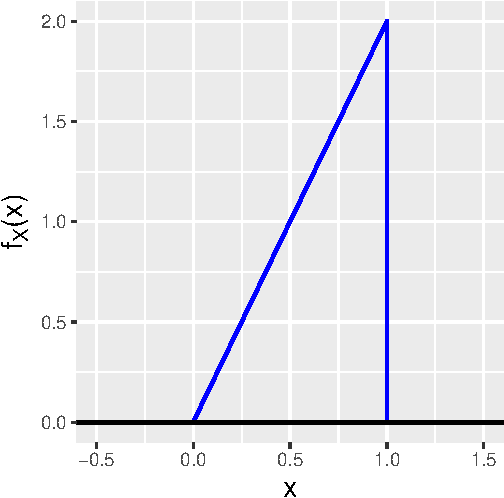
\includegraphics[keepaspectratio]{01-probability_files/figure-latex/fig-twox-1.pdf}}

}

\caption{\label{fig-twox}The probability density function
\(f_X(x) = 2x\), for \(0 \leq x \leq 1\).}

\end{figure}%

\begin{quote}
This pdf helps to illustrate many of the points made above. Note that it
is (a) non-negative and although its maximum value is \(> 1\), (b) it
integrates \textgreater{} to 1. (We need not actually integrate here, as
geometry is sufficient: the area under the curve is 1/2 \(\times\) 1
\(\times\) 2 = 1.)
\end{quote}

\begin{quote}
How would one interpret this pdf? Where its value is larger, we are more
likely to sample data. Full stop. What is the probability of sampling a
datum between 0 and 1/2? Again, we can use geometry and see that the
area under the curve is 1/2 \(\times\) 1/2 \(\times\) 1 = 1/4. (Which
means the probability of sampling a datum between 1/2 and 1 must be
\(1 - 1/4 = 3/4\).)
\end{quote}

\begin{quote}
Let's extend this example a bit by adding a condition. For instance,
what is the probability of sampling a datum between 1/4 and 1/2,
\emph{given} that we sample a datum between 0 and 3/4? In analogy with
how we worked with conditional probabilities above, we can write that
\begin{align*}
P(1/4 \leq X \leq 1/2 \, \vert \, 0 \leq X \leq 3/4) &= \frac{P(1/4 \leq X \leq 1/2 \cap 0 \leq X \leq 3/4)}{P(0 \leq X \leq 3/4)}\\
&=  \frac{P(1/4 \leq X \leq 1/2)}{P(0 \leq X \leq 3/4)} \,.
\end{align*} (How does this differ from computing the unconditional
probability \(P(1/4 \leq X \leq 1/2)\)? Technically, it does
not\ldots we could write out a similar expression to the one above. But
we note that the denominator would be \(P(0 \leq X \leq 1) = 1\) and
thus it would ``go away.'') Using geometrical arguments, we should be
able to convince ourselves that the answer we seek is 1/3.
\end{quote}

\begin{quote}
One last point we will make here is that for a continuous distribution,
it is meaningless to compute \(P(X = a)\). For instance: \[
P\left(X = \frac{1}{2}\right) = \int_{1/2}^{1/2} 2 x dx = \left. x^2 \right|_{1/2}^{1/2} = \frac{1}{4} - \frac{1}{4} = 0 \,.
\] What are we to make of this? Recall that a pdf is a probability
\emph{density} function, and that one can think of it as having units of
probability per unit interval\ldots so one has to integrate the pdf over
an interval of length greater than zero to derive a non-zero probability
value.
\end{quote}

\subsubsection{Shape Parameters and Families of
Distributions}\label{shape-parameters-and-families-of-distributions}

\begin{quote}
In the previous example, the stated pdf was the stated pdf: there was no
means by which to change its shape. We can generalize it by utilizing a
\emph{shape parameter}: \[
f_X(x \vert \theta) = \left\{ \begin{array}{cl} \theta x^{\theta-1} & 0 \leq x \leq 1 \\ 0 & \mbox{otherwise} \end{array} \right. \,,
\] where in the previous example, \(\theta = 2\). It is conventional to
denote a population parameter or a set of such parameters with the Greek
letter \(\theta\) (theta, pronounced ``thay-tah''). Here, \(\theta\)
represents a single, constant parameter whose value is \(> 0\). (If
\(\theta\) were negative, for instance, \(f_X(x \vert \theta)\) would be
\(< 0\), which is not allowed!) \(f_X(x \vert \theta)\), with
\(\theta \in \Theta = (0,\infty)\), is perhaps confusingly dubbed a
\emph{family of distributions}. (One might think that a family would
refer to a set of different mathematical forms for pdfs, like
\(\theta x^{\theta-1}\) and \(e^{-x/\theta}/\theta\), etc., but it
actually refers to the fact that \(\theta\) can take on more than one
value, yielding a family of shapes as illustrated in
Figure~\ref{fig-family}.)
\end{quote}

\begin{figure}

\centering{

\pandocbounded{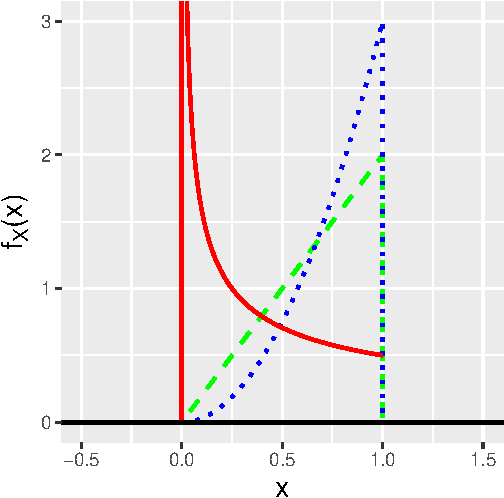
\includegraphics[keepaspectratio]{01-probability_files/figure-latex/fig-family-1.pdf}}

}

\caption{\label{fig-family}Examples of the family of pdfs
\(f_X(x \vert \theta) = \theta x^{\theta-1}\) for \(0 \leq x \leq 1\),
with parameters \(\theta =\) 1/2 (solid red line), 1 (dashed green
line), and 2 (dotted blue line).}

\end{figure}%

\subsubsection{A Simple Probability Mass
Function}\label{a-simple-probability-mass-function}

\begin{quote}
Let's play a game: we throw a dart at a board that has ten numbers on
it, 1 through 10. Assume that we are guaranteed to hit the board, and
that the regions associated with each number have the exact same size.
If we hit an even number, we get 0 points, while if we hit an odd
number, we get 2 points. Furthermore, if we hit a prime number, we get a
bonus of 1 point. What is the probability mass function for the number
of points we will score given a single throw of the dart?
\end{quote}

\begin{quote}
If we hit the 4, 6, 8, or 10, we get 0 points. (2 is prime, so we'd get
a bonus of 1 point by hitting that.) If we hit the 9, we get 2 points,
and if we hit the 1, 3, 5, or 7, we get 3 points. Hence the probability
mass function is
\end{quote}

{\def\LTcaptype{none} % do not increment counter
\begin{longtable}[]{@{}cc@{}}
\toprule\noalign{}
\(x\) & \(p_X(x)\) \\
\midrule\noalign{}
\endhead
\bottomrule\noalign{}
\endlastfoot
0 & 4/10 \\
1 & 1/10 \\
2 & 1/10 \\
3 & 4/10 \\
\end{longtable}
}

\begin{quote}
We see that this pmf is (a) non-negative and (b) has values \(p_X(x)\)
that lie between 0 and 1. Because we are dealing with masses and not
densities, probability calculations involve summations (while taking
care to note whether one or both limits of summation lie at a mass, and
if so, whether or not the inequality is, e.g., \(>\) or \(\geq\)). For
instance, what is the probability of achieving a score greater than 1
point? \(P(X > 1) =
p_X(2) + p_X(3) = 1/2\). What about a score of 3 points, given a score
greater than 0 points? \begin{align*}
P(X = 3 \vert X > 0) &= \frac{P(X = 3 \cap X > 0)}{P(X > 0)} = \frac{P(X = 3)}{P(X > 0)}\\
&= \frac{p_X(3)}{p_X(1)+p_X(2)+p_X(3)} = \frac{4}{1+1+4} = \frac{2}{3} \,.
\end{align*}
\end{quote}

\subsubsection{A More Complex Example Involving Both Masses and
Densities}\label{a-more-complex-example-involving-both-masses-and-densities}

\begin{quote}
There is no reason why masses and densities cannot be combined into a
single probability distribution. For instance, perhaps we have the
following: \[
h_X(x) = \left\{ \begin{array}{cc} 1/2 & x \in [0,1] \\ 1/2 & x = 2 \end{array} \right. \,.
\] There is nothing special about this function; the mathematics of
probability calculations is just a tad more complicated than before. For
instance, what is the probability of sampling a value greater than 3/4?
\[
P(X > 3/4) = \int_{3/4}^1 h_X(x) dx + h_X(2) = \frac{1}{2} \left. x \right|_{3/4}^1 + \frac{1}{2} = \frac{1}{8} + \frac{1}{2} = \frac{5}{8} \,.
\] Integrate over the domain(s) where densities are defined and sum over
the domain(s) where masses are defined. Done!
\end{quote}

\section{Probability Distributions: Expected Value and
Variance}\label{sec-chap1expected}

What to take away from this section:

\begin{itemize}
\item
  To characterize (or summarize the information contained in) a
  probability distribution, we can report\ldots{}

  \begin{itemize}
  \item
    the average value of a set of data sampled according to that
    distribution, i.e., the \emph{expected value} (or
    \emph{expectation})
  \item
    the width of the region of the real-number line in which data
    sampled according to a distribution are concentrated, i.e., the
    \emph{standard deviation} (or relatedly, the \emph{variance})
  \end{itemize}
\end{itemize}

A probability distribution represents the rates of occurrence of
different experimental outcomes. Can we determine an ``average''
outcome? In other words, can we determine what value to expect when we
next run the experiment? The answer is yes: this is the \emph{expected
value} of a random variable (or \emph{expectation}) and it is the
weighted average of all possible experimental outcomes: \begin{align*}
E[X] &= \frac{\sum_x x p_X(x)}{\sum_x p_X(x)} = \sum_x x p_X(x) ~~ \mbox{(discrete r.v.)} \\
     &= \frac{\int_x x f_X(x) dx}{\int_x f_X(x) dx} = \int_x x f_X(x) dx ~~ \mbox{(continuous r.v.)} \,.
\end{align*} In each case, the denominator disappears because it equals
1, by definition. Note that Greek letter \(\mu\) (mu, pronounced
``myoo''), which conventionally denotes the mean value of a pdf or pmf,
is also sometimes used interchangeably with \(E[X]\). See
Figure~\ref{fig-exvx}.

It is important here to note the following:

\begin{enumerate}
\def\labelenumi{\arabic{enumi}.}
\tightlist
\item
  The input to the expected value operator is (usually!) a random
  variable, so that input is capitalized. In other words, we always
  write \(E[X]\) and not \(E[x]\). (\(x\) is just a coordinate on the
  real-number line\ldots its expected value is simply \(x\) itself. See
  ``Expected Value Tricks'' in the examples below.)
\item
  \emph{The expected value is a constant; it is not random!} For any
  given pmf or pdf, the average value of a sampled datum does not change
  from experiment to experiment\ldots there is no randomness.
\end{enumerate}

Now, because the expected value is simply a weighted average, we can
write down a more general expression for it: \begin{align*}
E[g(X)] &= \frac{\sum_x g(x)p_X(x)}{\sum_x p_X(x)} = \sum_x g(x) p_X(x) ~~ \mbox{(discrete r.v.)} \\
        &= \frac{\int_x g(x)f_X(x) dx}{\int_x f_X(x) dx} = \int_x g(x) f_X(x) dx ~~ \mbox{(continuous r.v.)} \,.
\end{align*} This has been dubbed the ``Law of the Unconscious
Statistician'' (e.g., Ross (1988), as noted by Casella and Berger
(2002)) due to the fact that we all think of it as a
definition\ldots and not the result of a theorem.

A probability distribution may have an extended domain (e.g.,
\([0,\infty)\)) but often the probability mass or density is
concentrated in a relatively small interval. A metric that represents
the square of the ``width'' of that interval is the \emph{variance},
which is defined as \[
V[X] = \sigma^2 = E[(X-\mu)^2] = E[X^2] - (E[X])^2 \,.
\] The ``width'' itself\(-\)the square root of the variance\(-\)is
dubbed the \emph{standard deviation} and is denoted with the Greek
letter \(\sigma\) (``sigma,'' pronounced ``SIG-muh''). Note that because
the variance is the expected value of a squared quantity, it is always
non-negative. (And like the expected value, it is a \emph{constant}.)
See Figure~\ref{fig-exvx}.

\begin{figure}

\begin{minipage}[t]{0.50\linewidth}

\centering{

\pandocbounded{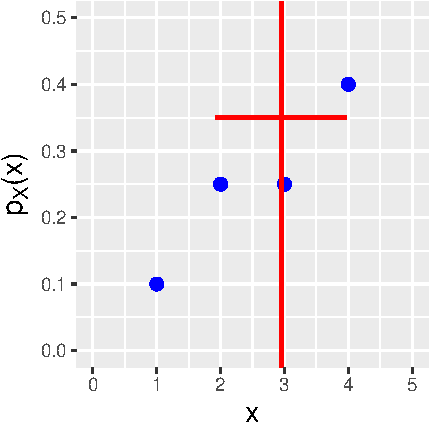
\includegraphics[keepaspectratio]{01-probability_files/figure-latex/fig-exvx-1.pdf}}

}

\subcaption{\label{fig-exvx-1}}

\end{minipage}%
%
\begin{minipage}[t]{0.50\linewidth}

\centering{

\pandocbounded{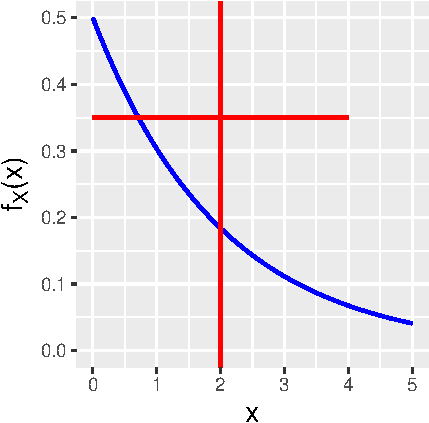
\includegraphics[keepaspectratio]{01-probability_files/figure-latex/fig-exvx-2.pdf}}

}

\subcaption{\label{fig-exvx-2}}

\end{minipage}%

\caption{\label{fig-exvx}Examples of a probability mass function (a) and
a probability density function (b), with the expected values \(E[X]\)
indicated by the vertical lines and the distribution widths (here,
\(E[X]-\sqrt{V[X]}\) to \(E[X]+\sqrt{V[X]}\)) indicated by the
horizontal lines.}

\end{figure}%

Both the expected value and variance are examples of \emph{moments} of
probability distributions. Moments represent elements of a
distribution's location and shape. In the end, moments are ``just''
expected values computed via the Law of the Unconscious Statistician,
ones that are defined around the coordinate origin (\(E[X^k]\)), and
ones that are defined around the distribution's mean, \(\mu\)
(\(E[(X-\mu)^k]\)). Other metrics used to describe a probability
distribution, such as its \emph{skewness}, are also related to moments.
(One definition of skewness is Fisher's moment coefficient:
\(E[(X-\mu)^3]/\sigma^3\).)

\subsection{Examples}\label{examples-4}

\subsubsection{Expected Value Tricks}\label{expected-value-tricks}

\begin{quote}
The expected value operator \(E[X]\) has the following properties.
\end{quote}

\begin{quote}
\begin{enumerate}
\def\labelenumi{\arabic{enumi}.}
\tightlist
\item
  If we multiply \(X\) by a constant \(a\), that constant can be moved
  out of the operator, i.e., \[
  E[aX] = aE[X] \,.
  \]
\item
  The expected value of a constant is simply that constant, i.e., \[
  E[b] = b \,.
  \]
\item
  The expected value operator is a linear operator, which means that we
  can split it at \(+\)'s and \(-\)'s, with the sign being preserved: \[
  E[aX - b] = E[aX] - E[b] = aE[X] - b \,.
  \]
\end{enumerate}
\end{quote}

\begin{quote}
If, for example, we define a random variable \(Y = 10X - 5\) and we know
that \(E[X] = 4\), then we can write that \(E[Y] = 10E[X] - 5 = 35\).
\end{quote}

\begin{quote}
Note that we have said nothing about \(E[XY]\) here. In general, we
cannot simplify this expression at all, \emph{unless} \(X\) and \(Y\)
are independent random variables (a concept we haven't discussed yet),
in which case \(E[XY] = E[X]E[Y]\).
\end{quote}

\subsubsection{Variance Tricks}\label{variance-tricks}

\begin{quote}
The variance operator \(V[X]\) has the following properties.
\end{quote}

\begin{quote}
\begin{enumerate}
\def\labelenumi{\arabic{enumi}.}
\tightlist
\item
  If we multiply \(X\) by a constant \(a\), that constant can be moved
  out of the operator, but it is then squared, i.e., \[
  V[aX] = a^2V[X] \,.
  \]
\item
  The variance of a constant is zero: \[
  V[b] = 0 \,.
  \]
\item
  The variance operator is a linear operator, which means that we can
  split it at \(+\)'s and \(-\)'s, with all signs becoming
  \emph{positive}: \[
  V[aX - b] = V[aX] + V[b] = a^2V[X] + 0 = a^2V[X] \,.
  \]
\end{enumerate}
\end{quote}

\begin{quote}
If, again, \(Y = 10X - 5\), and if \(V[X] = 2\), then
\(V[Y] = 100V[X] = 200\).
\end{quote}

\subsubsection{The Shortcut Formula for
Variance}\label{the-shortcut-formula-for-variance}

\begin{quote}
Above, we indicate that \[
V[X] = E[(X-\mu)^2] = E[X^2] - (E[X])^2 \,.
\] This is the so-called \emph{shortcut formula} for determining the
variance of a distribution. We can derive it as follows, making use of
the ``tricks'' we show above: \begin{align*}
V[X] = E[(X-\mu)^2] &= E[X^2 - 2X\mu + \mu^2] ~~\mbox{(expand)} \\
&= E[X^2] - E[2X\mu] + E[\mu^2] ~~\mbox{(split on + and -)} \\
&= E[X^2] - 2\mu E[X] + \mu^2 ~~\mbox{(slide constants out)}\\
&= E[X^2] - 2(E[X])^2 + (E[X])^2 = E[X^2] - (E[X])^2 \,,
\end{align*} where in the last line we make use of the fact that
\(E[X] = \mu\). Note what this shortcut formula means: it means that to
compute a variance, it is sufficient to compute both \(E[X]\) and
\(E[X^2]\) and combine the results. It also means that if we are given
any two of the quantities \(E[X]\), \(E[X^2]\), and \(V[X]\), we can
immediately derive the third one.
\end{quote}

\subsubsection{The Expected Value and Variance of a Probability Density
Function}\label{the-expected-value-and-variance-of-a-probability-density-function}

\begin{quote}
In the last section, we define the pdf \[
f_X(x \vert \theta) = \left\{ \begin{array}{cl} \theta x^{\theta-1} & 0 \leq x \leq 1 \\ 0 & \mbox{otherwise} \end{array} \right. \,,
\] For this pdf, the expected value is \[
E[X] = \int_0^1 x f_X(x) dx = \int_0^1 \theta x^\theta dx = \frac{\theta}{\theta+1} \left. x^{\theta+1} \right|_0^1 = \frac{\theta}{\theta+1} \,.
\] As for the variance, we utilize the shortcut formula, which means
that we compute \(E[X^2]\) first: \[
E[X^2] = \int_0^1 x^2 f_X(x) dx = \int_0^1 \theta x^{\theta+1} dx = \frac{\theta}{\theta+2} \left. x^{\theta+2} \right|_0^1 = \frac{\theta}{\theta+2} \,.
\] Hence the variance is \[
V[X] = E[X^2] - (E[X])^2 = \frac{\theta}{\theta+2} - \frac{\theta^2}{(\theta+1)^2} = \frac{\theta}{(\theta+2)(\theta+1)^2} \,.
\]
\end{quote}

\begin{quote}
We see that the value for our new pdf is similar: 0.643.
\end{quote}

\section{Probability Distributions: Working with
R}\label{sec-chap1working}

What to take away from this section:

\begin{itemize}
\item
  The programming language \texttt{R} is a tool by which the reader can,
  e.g.,

  \begin{itemize}
  \item
    visualize probability mass and density functions; and
  \item
    utilize numerical integration to carry out probability calculations.
  \end{itemize}
\end{itemize}

In this section, we introduce \texttt{R} as a tool with which to, e.g.,
visualize and numerically manipulate probability distributions. (Readers
who are looking for a somewhat broader, yet ultimately still concise,
introduction to \texttt{R} can find it
\href{https://cmu-intro-r.github.io}{here}.)

We start with the concept of the \emph{vector}:

\begin{Shaded}
\begin{Highlighting}[]
\NormalTok{x }\OtherTok{\textless{}{-}} \FunctionTok{c}\NormalTok{(}\StringTok{"Hello, world!"}\NormalTok{)}
\end{Highlighting}
\end{Shaded}

(The reader should feel free to open \texttt{R} and type in these lines
at the \texttt{Console} prompt.) In this example, we define a vector of
character strings which we name \texttt{x}; here, \texttt{x} has length
1:

\begin{Shaded}
\begin{Highlighting}[]
\FunctionTok{length}\NormalTok{(x)}
\end{Highlighting}
\end{Shaded}

\begin{verbatim}
[1] 1
\end{verbatim}

\texttt{c()} is an \texttt{R} function whose arguments (e.g.,
\texttt{"Hello,\ world!"}) are what are to be the constituents of the
vector. The arrow is an assignment operator; \texttt{=} is equally
valid. We can create a numeric vector as follows:

\begin{Shaded}
\begin{Highlighting}[]
\NormalTok{x }\OtherTok{\textless{}{-}} \FunctionTok{c}\NormalTok{(}\DecValTok{1}\NormalTok{, }\DecValTok{2}\NormalTok{, }\DecValTok{4}\NormalTok{, }\DecValTok{8}\NormalTok{)}
\FunctionTok{print}\NormalTok{(x)}
\end{Highlighting}
\end{Shaded}

\begin{verbatim}
[1] 1 2 4 8
\end{verbatim}

\begin{Shaded}
\begin{Highlighting}[]
\FunctionTok{length}\NormalTok{(x)}
\end{Highlighting}
\end{Shaded}

\begin{verbatim}
[1] 4
\end{verbatim}

but when the numbers follow a (long) sequence, it can be easier to
utilize \texttt{seq()}:

\begin{Shaded}
\begin{Highlighting}[]
\NormalTok{x }\OtherTok{\textless{}{-}} \FunctionTok{seq}\NormalTok{(}\DecValTok{0}\NormalTok{, pi, }\AttributeTok{by =} \FloatTok{0.01}\NormalTok{)  }\CommentTok{\# 0, 0.01, 0.02, ..., 3.14 (but not 3.15)}
                            \CommentTok{\# pi and Inf are built{-}in constants}
\FunctionTok{length}\NormalTok{(x)}
\end{Highlighting}
\end{Shaded}

\begin{verbatim}
[1] 315
\end{verbatim}

When it comes to probability distributions, what might we want to do
first?

Let's suppose that our data are sampled from this pdf: \[
f_X(x) = \left\{ \begin{array}{cl} c x \sin x & 0 \leq x \leq \pi \\ 0 & \mbox{otherwise} \end{array} \right. \,,
\] \(c\) is a \emph{normalization constant}, meaning it has some value
(to be determined) such that the integral of \(f_X(x)\) from 0 to
\(\pi\) is 1. Below, we will show how we can determine the value of
\(c\) using \texttt{R} code. But first, we will assume \(c = 1\) and
determine if \(f_X(x)\) is non-negative (as it should be!):

\begin{Shaded}
\begin{Highlighting}[]
\NormalTok{x   }\OtherTok{\textless{}{-}} \FunctionTok{seq}\NormalTok{(}\DecValTok{0}\NormalTok{, pi, }\AttributeTok{by =}\NormalTok{ pi }\SpecialCharTok{/} \DecValTok{100}\NormalTok{)}
\NormalTok{f.x }\OtherTok{\textless{}{-}}\NormalTok{ x }\SpecialCharTok{*} \FunctionTok{sin}\NormalTok{(x)            }
\FunctionTok{min}\NormalTok{(f.x)}
\end{Highlighting}
\end{Shaded}

\begin{verbatim}
[1] 0
\end{verbatim}

Note how we do not have to use a \texttt{for}-loop here, as one of the
hallmarks of \texttt{R} is \emph{vectorization}: if \texttt{R} sees that
\texttt{x} is a vector, it will work with the vector directly and thus
\texttt{f.x} will itself be a vector with the same length as \texttt{x}
(and with the first element of \texttt{x} corresponding to the first
element of \texttt{f.x}, etc.). We see that the minimum value is 0.

If we want to go further, we can make a simple plot (see
Figure~\ref{fig-xsinx}):

\begin{figure}

\centering{

\pandocbounded{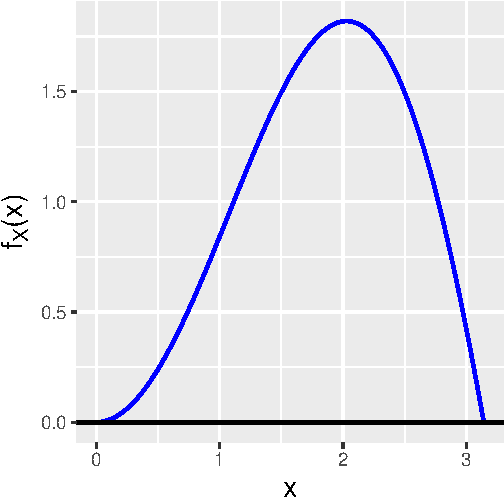
\includegraphics[keepaspectratio]{01-probability_files/figure-latex/fig-xsinx-1.pdf}}

}

\caption{\label{fig-xsinx}The function \(x \sin x\).}

\end{figure}%

The \texttt{ggplot()} function puts \texttt{x} on the \(x\)-axis and
\texttt{f.x} on the \(y\)-axis. We then connect each point with a line
(\texttt{geom\_line()}), make the line blue (\texttt{col\ =\ "blue"}),
overlay a horizontal red line at \(y = 0\) (\texttt{geom\_hline()}, with
\texttt{yintercept\ =\ 0}), and change the default \(y\)-axis label to
one that includes the subscript ``X'' (\texttt{labs()}).

The next step is to determine the normalization constant. Let's suppose
that we have forgotten integration by parts and thus we are not sure how
to integrate \(f_X(x)\). We can code numerical integration in \texttt{R}
using a combination of a function that evaluates \(f_X(x)\) and a call
to the built-in function \texttt{integrate()}, which performs numerical
integration:

\begin{Shaded}
\begin{Highlighting}[]
\NormalTok{f }\OtherTok{\textless{}{-}} \ControlFlowTok{function}\NormalTok{(x) \{}
  \FunctionTok{return}\NormalTok{(x }\SpecialCharTok{*} \FunctionTok{sin}\NormalTok{(x))}
\NormalTok{\}}
\FunctionTok{integrate}\NormalTok{(f, }\DecValTok{0}\NormalTok{, pi) }\CommentTok{\# integrate the function f between 0 and pi}
\end{Highlighting}
\end{Shaded}

\begin{verbatim}
3.141593 with absolute error < 3.5e-14
\end{verbatim}

\begin{quote}
We see that the integral is \(\pi\), so to make the pdf valid, we have
to set \(c\) to \(1/\pi\): \[
f_X(x) = \left\{ \begin{array}{cl} \frac{1}{\pi} x \sin x & 0 \leq x \leq \pi \\ 0 & \mbox{otherwise} \end{array} \right. \,.
\]
\end{quote}

Let's suppose we sample data from this distribution. What is the
probability that the next observed datum will have a value between 1 and
2? We can use \texttt{integrate} to figure that out:

\begin{Shaded}
\begin{Highlighting}[]
\NormalTok{f }\OtherTok{\textless{}{-}} \ControlFlowTok{function}\NormalTok{(x) \{}
  \FunctionTok{return}\NormalTok{(x }\SpecialCharTok{*} \FunctionTok{sin}\NormalTok{(x) }\SpecialCharTok{/}\NormalTok{ pi)     }\CommentTok{\# we now include the normalization constant}
\NormalTok{\}}
\FunctionTok{integrate}\NormalTok{(f, }\DecValTok{1}\NormalTok{, }\DecValTok{2}\NormalTok{) }\CommentTok{\# integrate the function f between 1 and 2}
\end{Highlighting}
\end{Shaded}

\begin{verbatim}
0.4585007 with absolute error < 5.1e-15
\end{verbatim}

The answer is 0.4585\ldots there is a 45.85\% chance that the next datum
will have a value between 1 and 2.

What is the expected value, \(E[X]\), of \(f_X(x)\)?

\begin{Shaded}
\begin{Highlighting}[]
\NormalTok{f }\OtherTok{\textless{}{-}} \ControlFlowTok{function}\NormalTok{(x) \{}
  \FunctionTok{return}\NormalTok{(x}\SpecialCharTok{\^{}}\DecValTok{2} \SpecialCharTok{*} \FunctionTok{sin}\NormalTok{(x) }\SpecialCharTok{/}\NormalTok{ pi)     }\CommentTok{\# add an additional x}
\NormalTok{\}}
\FunctionTok{integrate}\NormalTok{(f, }\DecValTok{0}\NormalTok{, pi)}
\end{Highlighting}
\end{Shaded}

\begin{verbatim}
1.868353 with absolute error < 2.1e-14
\end{verbatim}

The expected value is 1.868. Given the appearance of the pdf, this
number makes sense.

\subsection{Examples}\label{examples-5}

\subsubsection{Numerical Integration and Conditional
Probability}\label{numerical-integration-and-conditional-probability}

\begin{quote}
Let's suppose that we would like to numerically evaluate \[
P(1 \leq X \leq 2 \vert X > 0.5) = \frac{P(1 \leq X \leq 2 \cap X > 0.5)}{P(X > 0.5} = \frac{P(1 \leq X \leq 2)}{P(X > 0.5} \,.
\] As we have already defined At first, it would appear that all we have
to do is to call \texttt{integrate()} twice
\end{quote}

\begin{Shaded}
\begin{Highlighting}[]
\NormalTok{f }\OtherTok{\textless{}{-}} \ControlFlowTok{function}\NormalTok{(x) \{}
  \FunctionTok{return}\NormalTok{(x }\SpecialCharTok{*} \FunctionTok{sin}\NormalTok{(x) }\SpecialCharTok{/}\NormalTok{ pi)}
\NormalTok{\}}
\FunctionTok{integrate}\NormalTok{(f, }\DecValTok{1}\NormalTok{, }\DecValTok{2}\NormalTok{) }\SpecialCharTok{/} \FunctionTok{integrate}\NormalTok{(f, }\FloatTok{0.5}\NormalTok{, pi)}
\end{Highlighting}
\end{Shaded}

\begin{quote}
However, this will not work, since \texttt{integrate()} returns a
\emph{list}, not a single numerical value. So we have to figure out
where the value of the integral value is stored:
\end{quote}

\begin{Shaded}
\begin{Highlighting}[]
\FunctionTok{names}\NormalTok{(}\FunctionTok{integrate}\NormalTok{(f, }\DecValTok{1}\NormalTok{, }\DecValTok{2}\NormalTok{))  }\CommentTok{\# return the names of each list element}
\end{Highlighting}
\end{Shaded}

\begin{verbatim}
[1] "value"        "abs.error"    "subdivisions" "message"      "call"        
\end{verbatim}

\begin{quote}
What we want is \texttt{value}. To reference the value directly, we use
a dollar sign, as shown here:
\end{quote}

\begin{Shaded}
\begin{Highlighting}[]
\FunctionTok{integrate}\NormalTok{(f, }\DecValTok{1}\NormalTok{, }\DecValTok{2}\NormalTok{)}\SpecialCharTok{$}\NormalTok{value }\SpecialCharTok{/} \FunctionTok{integrate}\NormalTok{(f, }\FloatTok{0.5}\NormalTok{, pi)}\SpecialCharTok{$}\NormalTok{value}
\end{Highlighting}
\end{Shaded}

\begin{verbatim}
[1] 0.3836833
\end{verbatim}

\begin{quote}
Done. Our conditional probability is 0.4645.
\end{quote}

\subsubsection{Numerical Integration and
Variance}\label{numerical-integration-and-variance}

\begin{quote}
Above, we compute the expected value of \(f_X(x)\). For the variance, we
adapt the same code to compute \(E[X^2]\), then utilize the shortcut
formula:
\end{quote}

\begin{Shaded}
\begin{Highlighting}[]
\NormalTok{f }\OtherTok{\textless{}{-}} \ControlFlowTok{function}\NormalTok{(x) \{}
  \FunctionTok{return}\NormalTok{(x}\SpecialCharTok{\^{}}\DecValTok{2} \SpecialCharTok{*} \FunctionTok{sin}\NormalTok{(x) }\SpecialCharTok{/}\NormalTok{ pi)     }\CommentTok{\# same code as above}
\NormalTok{\}}
\NormalTok{E.X }\OtherTok{\textless{}{-}} \FunctionTok{integrate}\NormalTok{(f, }\DecValTok{0}\NormalTok{, pi)}\SpecialCharTok{$}\NormalTok{value}

\NormalTok{f }\OtherTok{\textless{}{-}} \ControlFlowTok{function}\NormalTok{(x) \{}
  \FunctionTok{return}\NormalTok{(x}\SpecialCharTok{\^{}}\DecValTok{3} \SpecialCharTok{*} \FunctionTok{sin}\NormalTok{(x) }\SpecialCharTok{/}\NormalTok{ pi)     }\CommentTok{\# add one more power of x}
\NormalTok{\}}
\NormalTok{V.X }\OtherTok{\textless{}{-}} \FunctionTok{integrate}\NormalTok{(f, }\DecValTok{0}\NormalTok{, pi)}\SpecialCharTok{$}\NormalTok{value }\SpecialCharTok{{-}}\NormalTok{ E.X}\SpecialCharTok{\^{}}\DecValTok{2}
\NormalTok{V.X }
\end{Highlighting}
\end{Shaded}

\begin{verbatim}
[1] 0.3788611
\end{verbatim}

\begin{Shaded}
\begin{Highlighting}[]
\FunctionTok{sqrt}\NormalTok{(V.X)}
\end{Highlighting}
\end{Shaded}

\begin{verbatim}
[1] 0.6155169
\end{verbatim}

\begin{quote}
The variance is 0.379 and the standard deviation is 0.616. We interpret
these numbers as saying that the majority of the observed data will lie
between \(1.868 - 0.616 = 1.252\) and \(1.868 + 0.616 = 2.484\). If we
recall introductory statistics, the proportion of values within one
standard deviation of the mean for a normal distribution (i.e., a bell
curve) is 0.683\ldots but that value changes from distribution to
distribution. What is the value here?
\end{quote}

\begin{Shaded}
\begin{Highlighting}[]
\NormalTok{f }\OtherTok{\textless{}{-}} \ControlFlowTok{function}\NormalTok{(x) \{}
  \FunctionTok{return}\NormalTok{(x }\SpecialCharTok{*} \FunctionTok{sin}\NormalTok{(x) }\SpecialCharTok{/}\NormalTok{pi)       }\CommentTok{\# back to the original pdf}
\NormalTok{\}}
\FunctionTok{integrate}\NormalTok{(f, E.X }\SpecialCharTok{{-}} \FunctionTok{sqrt}\NormalTok{(V.X), E.X }\SpecialCharTok{+} \FunctionTok{sqrt}\NormalTok{(V.X))}\SpecialCharTok{$}\NormalTok{value}
\end{Highlighting}
\end{Shaded}

\begin{verbatim}
[1] 0.642609
\end{verbatim}

\begin{quote}
We see that the value for our new pdf is similar: 0.643.
\end{quote}

\section{Probability Distributions: Cumulative Distribution
Function}\label{sec-chap1cumulative}

What to take away from this section:

\begin{itemize}
\item
  An alternative means by which to encapsulate the information contained
  in a probability distribution is the \emph{cumulative distribution
  function} or \emph{cdf}.
\item
  Foreshadowing: cumulative distribution functions play a fundamental
  role in statistical inference, particularly when we construct
  \emph{confidence intervals} and perform \emph{hypothesis tests}.
\end{itemize}

A cumulative distribution function (a cdf) is another means by which to
mathematically express a probability distribution, which is to say, if
we have a cdf, we can derive the associated pmf/pdf and vice-versa. A
cdf is, in the discrete case, a sum of probability masses that lie to
the left of a chosen coordinate \(x\) on the real-number line, \[
F_X(x) = \sum_{y \leq x} p_Y(y) \,,
\] while in the continuous case it is an integral of the probability
density that lies to the left of \(x\): \[
F_X(x) = \int_{y \leq x} f_Y(y) dy \,.
\] In both cases, we utilize a dummy variable for the pmf/pdf itself
because \(x\) is the upper limit of summation/integration. See
Figure~\ref{fig-pdfcdf}, which illustrates how a cdf ``collects'' all
the probability masses or density ``to the left'' of a given value of
\(x\). Given this figure, it should be clear that \(F_X(-\infty) = 0\)
(there is nothing to collect ``to the left'' of \(-\infty\)) and
\(F_X(\infty) = 1\) (since, by the time we reach \(x = \infty\),
\emph{all} masses or density have been collected). Another thing to keep
in mind is that even if a random variable is discrete, its associated
cdf \(F_X(x)\) is continuously valued, because it is defined at all
values of \(x\) (although it is technically not ``mathematically
continuous'' due to the steps that \(F_X(x)\) takes at each value of
\(x\) where there is a probability mass).

\begin{figure}

\begin{minipage}[t]{0.50\linewidth}

\centering{

\pandocbounded{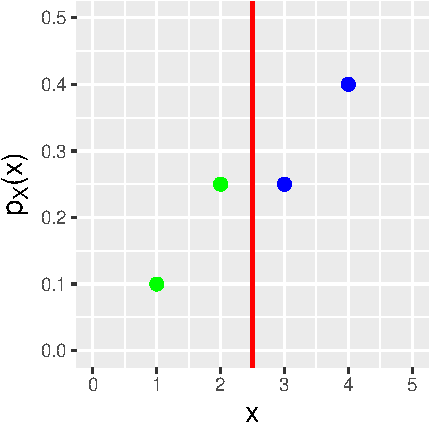
\includegraphics[keepaspectratio]{01-probability_files/figure-latex/fig-pdfcdf-1.pdf}}

}

\subcaption{\label{fig-pdfcdf-1}}

\end{minipage}%
%
\begin{minipage}[t]{0.50\linewidth}

\centering{

\pandocbounded{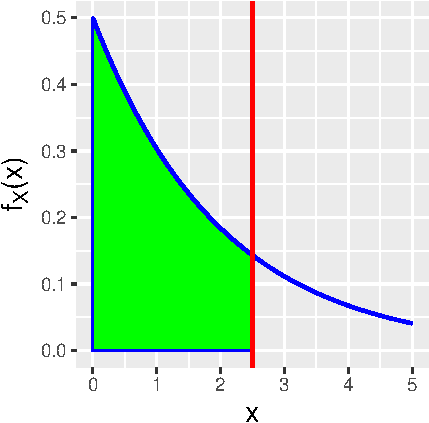
\includegraphics[keepaspectratio]{01-probability_files/figure-latex/fig-pdfcdf-2.pdf}}

}

\subcaption{\label{fig-pdfcdf-2}}

\end{minipage}%

\caption{\label{fig-pdfcdf}Illustration of the relationship between a
probability mass function (left) and a probability density function
(right) and its associated cdf (evaluated here at \(x = 2.5\)). For the
pmf, the cdf is the sum of the probability masses to the left of
\(x = 2.5\) (the masses marked in green), while for the pdf, the cdf is
the integral over \(x \in [0,2.5]\) (the area under curve shown in
green).}

\end{figure}%

\begin{figure}

\begin{minipage}[t]{0.50\linewidth}

\centering{

\pandocbounded{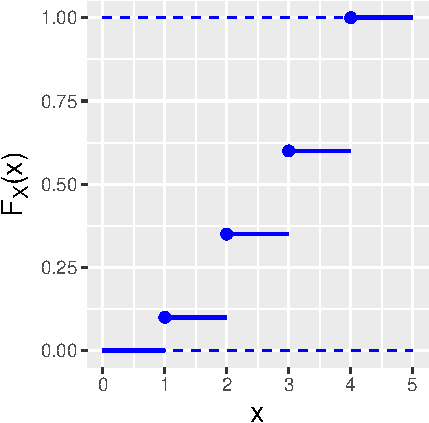
\includegraphics[keepaspectratio]{01-probability_files/figure-latex/fig-cdfs-1.pdf}}

}

\subcaption{\label{fig-cdfs-1}}

\end{minipage}%
%
\begin{minipage}[t]{0.50\linewidth}

\centering{

\pandocbounded{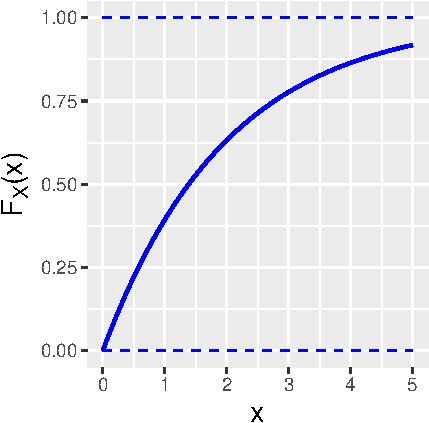
\includegraphics[keepaspectratio]{01-probability_files/figure-latex/fig-cdfs-2.pdf}}

}

\subcaption{\label{fig-cdfs-2}}

\end{minipage}%

\caption{\label{fig-cdfs}Examples of the cdfs \(F_X(x)\) for the
probability mass function (left) and the probability density function
(right) shown in Figure~\ref{fig-pdfcdf}.}

\end{figure}%

A cdf is useful to have when our goal is to compute the probability of
that the value of a sampled random variable lies between \(x = a\) and
\(x = b\). For the case of a continuous random variable, \[
P(a < X < b) = F_X(b) - F_X(a) \,.
\] As we can see, if we have the cdf, we do not need to perform
integration to compute the probability\ldots we just plug in coordinate
values. (Note that the form of the inequality, i.e., whether we have
\(<\) or \(\leq\), does not matter.) However, when we are dealing with a
discrete random variable, we need to tread far more carefully, because
the form of the inequality can matter. Let's suppose we have a pmf with
masses given at \(x = \{0,1\}\). Then, e.g., \begin{align*}
P(0 \leq X \leq 1) &= \sum_{x \in [0,1]} p_X(x) = p_X(0) + p_X(1) = F_X(1) \\
P(0 < X \leq 1) &= \sum_{x \in (0,1]} p_X(x) = p_X(1) = F_X(1) - F_X(0) \\
P(0 < X < 1) &= \sum_{x \in (0,1)} p_X(x) = 0 \,.
\end{align*}

\begin{figure}

\centering{

\pandocbounded{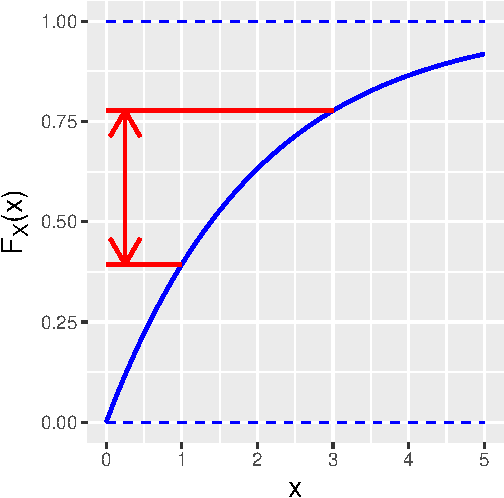
\includegraphics[keepaspectratio]{01-probability_files/figure-latex/fig-pmfcdf-1.pdf}}

}

\caption{\label{fig-pmfcdf}An illustration of the relationship between a
cdf and probability. The probability \(P(1 < X < 3)\) is given by the
distance between the two red lines (i.e., \(F_X(3)-F_X(1)\)).}

\end{figure}%

We will make two final points here about cdfs.

First, as indicated above, given a cdf, we can find the associated
pmf/pdf. If a pmf has non-zero masses at values \(x - \Delta x\) and
\(x\), and none in between, then \[
p_X(x) = F_X(x) - F_X(x-\Delta x) \,,
\] while in the continuous case, \[
f_X(x) = \frac{d}{dx}F_X(x) \,,
\] assuming \(F_X(x)\) is differentiable at \(x\).

Second, we can define an inverse cumulative distribution function, or
inverse cdf. The inverse cdf takes as input the total probability
collected to the left of \(x\) (e.g., the green region shown in the
right panel of Figure~\ref{fig-pdfcdf}) and returns the associated value
of \(x\). In other words, if \(q = F_X(x)\), then \(x = F_X^{-1}(q)\).

One issue that arises with the inverse cdf is that if \(F_X(x)\) is not
strictly monotonically increasing (i.e., if for some range of values,
\(\frac{d}{dx}F_X(x) = 0\)) then there is no unique inverse. For
instance, see the left panel of Figure~\ref{fig-cdfs}: if we input
\(F_X(x) = 0.35\), then \(x \in [2,3)\). We can circumvent this issue by
utilizing the \emph{generalized inverse cdf} instead, for which \[
x = F_X^{-1}(q) = \mbox{inf}\{ x : F_X(x) \geq q \} \,.
\] The symbol ``inf'' indicates that we are finding the infimum, or
smallest value, of the indicated set of values. Here, the output \(x\)
is the smallest value for which \(F_X(x) \geq q\) holds. For our given
example, \(x = 2\). On the other hand, if we pick a value of \(F_X(x)\)
that lies \emph{between} the steps, we would choose the smallest \(x\)
value associated with the next higher step. For instance, if for our
example we want the inverse cdf for \(F_X(x) = 0.5\), which lies between
the steps at 0.35 and 0.6, we would take the smallest value of \(x\)
associated with \(F_X(x) = 0.6\), which is \(x = 3\). (Note that
\texttt{R} utilizes the generalized form of the inverse cdf.)

\subsection{Examples}\label{examples-6}

\subsubsection{The Cumulative Distribution Function for a Probability
Density
Function}\label{the-cumulative-distribution-function-for-a-probability-density-function}

\begin{quote}
We work again with our simple parameterized pdf: \[
f_X(x \vert \theta) = \left\{ \begin{array}{cl} \theta x^{\theta-1} & 0 \leq x \leq 1 \\ 0 & \mbox{otherwise} \end{array} \right. \,.
\] The cdf for this function is simply the integral of the pdf ``to the
left'' of the coordinate \(x\): \[
F_X(x \vert \theta) = \int_0^x f_Y(y \vert \theta) dy \,.
\] Because the upper bound of the integral is \(x\), we replace \(x\) in
the integrand with a dummy variable. (Here, \(y\) was chosen
arbitrarily.) Thus \[
F_X(x \vert \theta) = \int_0^x \theta y^{\theta-1} dy = \left. y^\theta \right|_0^x = x^\theta \,.
\] We can answer a variety of questions given this cdf. For
example\ldots{}
\end{quote}

\begin{quote}
\begin{enumerate}
\def\labelenumi{\arabic{enumi}.}
\tightlist
\item
  What is the median of this distribution?
\end{enumerate}

The median \(\tilde{x}\) is the point on the real-number line where \[
P(X \leq \tilde{x}) = \frac{1}{2} \,.
\] For our distribution, \[
\tilde{x}^\theta = \frac{1}{2} ~\Rightarrow~ \tilde{x} = \left( \frac{1}{2} \right)^{1/\theta} \,.
\]
\end{quote}

\begin{quote}
\begin{enumerate}
\def\labelenumi{\arabic{enumi}.}
\setcounter{enumi}{1}
\tightlist
\item
  Now let \(\theta = 3\). What is the probability of sampling a datum
  between \(x = 1/4\) and \(x = 3/4\)? \begin{align*}
  P\left(\frac{1}{4} \leq X \leq \frac{3}{4}\right) &= F_X\left(\frac{3}{4} \vert \theta=3\right) - F_X\left(\frac{1}{4} \vert \theta=3\right)\\
  &= \left(\frac{3}{4}\right)^3 - \left(\frac{1}{4}\right)^3 = \frac{26}{64} = \frac{13}{32} \,.
  \end{align*}
\end{enumerate}
\end{quote}

\subsubsection{Visualizing the Cumulative Distribution Function in
R}\label{visualizing-the-cumulative-distribution-function-in-r}

\begin{quote}
We continue with the pdf we use above, with \(\theta = 3\). To show the
region being integrated over to compute a cdf value, for say
\(x = 0.6\), we utilize \texttt{R}'s \texttt{polygon()} function. (See
Figure~\ref{fig-cdfpoly}.)
\end{quote}

\begin{figure}

\centering{

\pandocbounded{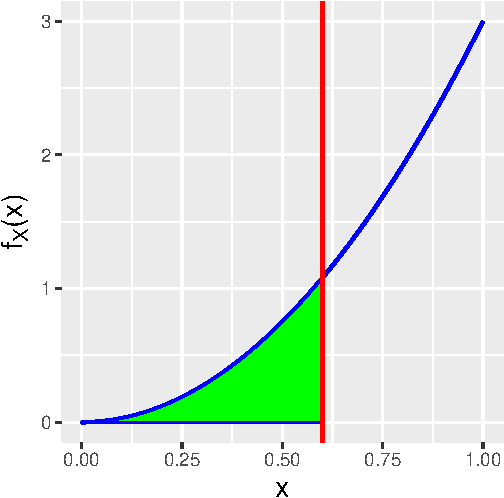
\includegraphics[keepaspectratio]{01-probability_files/figure-latex/fig-cdfpoly-1.pdf}}

}

\caption{\label{fig-cdfpoly}The cdf for \(f_X(x) = 3x^2\) at \(x = 0.6\)
is the area represented in green.}

\end{figure}%

\begin{quote}
What is happening in this code chunk? We first define a sequence of
values for \texttt{x} (via \texttt{seq()}), then compute the pdf for
each \texttt{x} value (\texttt{f.x}). We then define a data frame with
\texttt{x} and \texttt{f.x} as columns, and determine which rows
correspond to values of \texttt{x} that are less than or equal to 0.6
(via \texttt{subset()}). To create the polygon, we pass the subset data
frame \texttt{df.shade} to the function \texttt{geom\_area()}.
\end{quote}

\begin{quote}
If we wish to visualize the full cdf, we can do the following. (See
Figure~\ref{fig-cdfcurve}.)
\end{quote}

\begin{figure}

\centering{

\pandocbounded{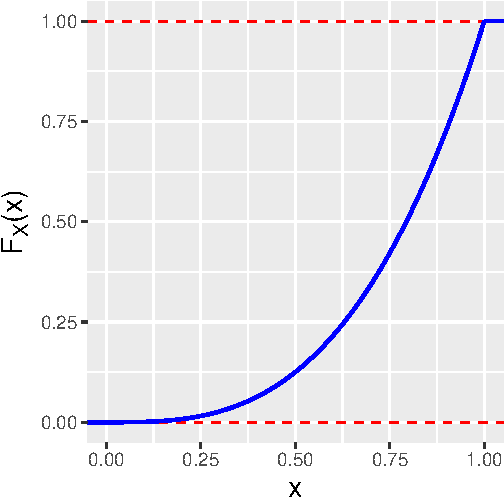
\includegraphics[keepaspectratio]{01-probability_files/figure-latex/fig-cdfcurve-1.pdf}}

}

\caption{\label{fig-cdfcurve}The cdf for \(f_X(x) = 3x^2\).}

\end{figure}%

\subsubsection{The CDF for a Mathematically Discontinuous
Distribution}\label{the-cdf-for-a-mathematically-discontinuous-distribution}

\begin{quote}
Assume that we are handed the following pdf: \[
f_X(x \vert \theta) = \left\{ \begin{array}{cl} 1/2 & 0 \leq x \leq 1 \\ 2-x & 1 \leq x \leq 2 \\ 0 & \mbox{otherwise} \end{array} \right. \,,
\] which we display in Figure~\ref{fig-discon}.
\end{quote}

\begin{figure}

\centering{

\pandocbounded{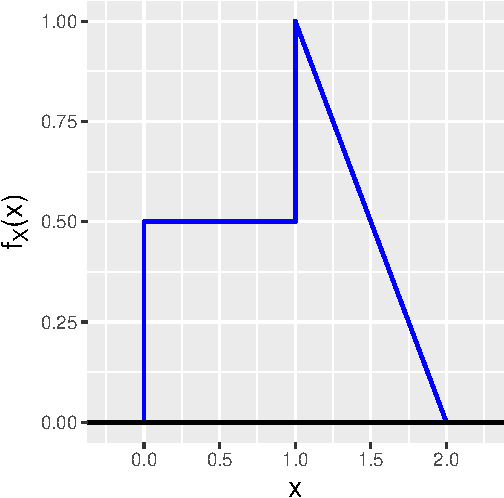
\includegraphics[keepaspectratio]{01-probability_files/figure-latex/fig-discon-1.pdf}}

}

\caption{\label{fig-discon}A continuous probability density function
that is mathematically discontinuous at \(x=1\).}

\end{figure}%

\begin{quote}
This is a completely valid, ``continuous'' pdf that has a mathematical
discontinuity at \(x = 1\). What is the cdf for this function?
\end{quote}

\begin{quote}
The key insight is that we should not try to evaluate the integral of
\(f_X(x)\) from 0 to \(x\) when \(x > 1\) with a single
integral\ldots this will not work! We simply have to break the problem
up so as to define the cdf over the domain {[}0,1), and then over the
domain {[}1,2{]}. \begin{align*}
F_X(x \vert x < 1) &= \int_0^x f_Y(y) dy = \frac{1}{2} \int_0^y dy = \frac{x}{2} \\
F_X(x \vert x \geq 1) &= \int_0^1 f_Y(y) dy + \int_1^x f_Y(y) dy = \left. \frac{y}{2} \right|_0^1 + \int_1^x (2-y) dy\\
&= \frac{1}{2} - \left. \frac{(2-y)^2}{2} \right|_1^x \\
&= \frac{1}{2} - \left( \frac{(2-x)^2}{2} - \frac{1}{2} \right) = 1 - \frac{(2-x)^2}{2} \,.
\end{align*} (Not sure if this is right? We can at the very least do
sanity checking, as we know \(F_X(1) = 1/2\) and
\(F_X(2) = 1\)\ldots and our formula produces these results!
Alternatively, we can take the derivative of \(F_X(x)\) and see if it
matches \(f_X(x)\).) We display the cdf in Figure~\ref{fig-disconcdf}.
\end{quote}

\begin{figure}

\centering{

\pandocbounded{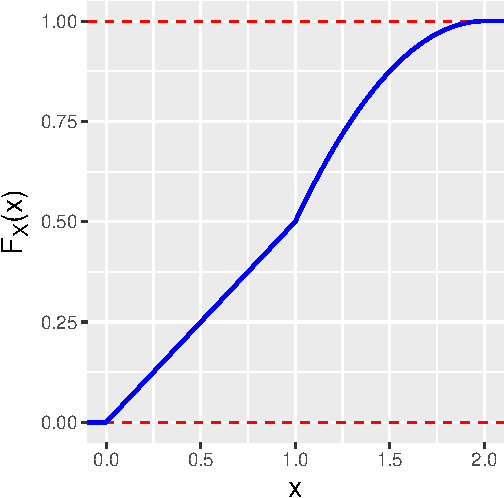
\includegraphics[keepaspectratio]{01-probability_files/figure-latex/fig-disconcdf-1.pdf}}

}

\caption{\label{fig-disconcdf}The cdf for our mathematically
discontinuous pdf.}

\end{figure}%

\section{The Law of Total Probability}\label{sec-chap1lotp}

What to take away from this section:

\begin{itemize}
\tightlist
\item
  When a parameter of a probability distribution is not actually a
  constant, but is itself a random variable, we utilize the \emph{law of
  total probability} so as to determine the distributions of observed
  data irrespective of the sampled value of the parameter.
\end{itemize}

One of the laws of probability that we introduce in
Section~\ref{sec-chap1further} is the Law of Total Probability, or LoTP:
if we partition a sample space \(\Omega\) into \(k\) disjoint events
\(\{B_1,\ldots,B_k\}\), then for any event \(A\) we can write \[
P(A) = \sum_{i=1}^k P(A \vert B_i) P(B_i) \,.
\] We are in a position now, having introduced random variables and
probability distributions, to update how we think of this law: it can
express the probability of a random variable \(X\) when it is sampled
from a discrete distribution with parameter \(\theta\)\ldots and when
\(\theta\) itself is not a fixed constant (as it has been up until now),
but \emph{is itself a discrete random variable}. To see this, let's
rewrite the LoTP given this description: \[
p_X(x) = \sum_\theta p_{X \vert \theta}(x \vert \theta) p_{\Theta}(\theta) \,.
\] This equation is saying that the probability mass associated with the
coordinate \(x\) is the value of the mass for \(x\), given the value
\(\theta\), weighted by the probability that we would even observe the
value \(\theta\) in the first place. Or, that \(p_X(x)\) is a weighted
average of the values of the conditional distribution
\(p_{X \vert \theta}(x \vert \theta)\), where the weights are given by
\(p_{\Theta}(\theta)\).

What if \(\theta\) is actually a continuous random variable? We can
extend the LoTP to handle that possibility by replacing the summation
over a discrete random variable with an integral over a continuous one:
\[
p_X(x) = \int_\theta p_{X \vert \theta}(x \vert \theta) f_{\Theta}(\theta) d\theta \,.
\] And what if the distribution of \(X \vert \theta\) is continuous? We
would just replace the \(p_X\) and the \(p_{X \vert \theta}\) in the
equations above with \(f_X\) and \(f_{X \vert \theta}\), i.e., we would
use the LoTP to define a probability density instead of a probability
mass.

\subsection{Examples}\label{examples-7}

\subsubsection{The LoTP With Two Simple Discrete
Distributions}\label{the-lotp-with-two-simple-discrete-distributions}

\begin{quote}
Let's suppose we have two random variables \(X\) and \(Y\), where the
probability mass function for \(Y\) is
\end{quote}

{\def\LTcaptype{none} % do not increment counter
\begin{longtable}[]{@{}cc@{}}
\toprule\noalign{}
\(y\) & \(p_Y(y)\) \\
\midrule\noalign{}
\endhead
\bottomrule\noalign{}
\endlastfoot
0 & 2/3 \\
1 & 1/3 \\
\end{longtable}
}

\begin{quote}
and where, if \(Y = 0\), the pmf for \(X\) is
\end{quote}

{\def\LTcaptype{none} % do not increment counter
\begin{longtable}[]{@{}cc@{}}
\toprule\noalign{}
\(x \vert y=0\) & \(p_{X \vert Y}(x \vert y=0)\) \\
\midrule\noalign{}
\endhead
\bottomrule\noalign{}
\endlastfoot
0 & 4/5 \\
1 & 1/5 \\
\end{longtable}
}

\begin{quote}
and if \(Y = 1\) the pmf for \(X\) is
\end{quote}

{\def\LTcaptype{none} % do not increment counter
\begin{longtable}[]{@{}cc@{}}
\toprule\noalign{}
\(x \vert y=1\) & \(p_{X \vert Y}(x \vert y=1)\) \\
\midrule\noalign{}
\endhead
\bottomrule\noalign{}
\endlastfoot
0 & 3/5 \\
1 & 2/5 \\
\end{longtable}
}

\begin{quote}
What is the pmf \(p_X(x)\)?
\end{quote}

\begin{quote}
The Law of Total Probability tells us that \[
p_X(x) = \sum_y p_{X \vert Y}(x \vert y) p_{Y}(y) \,,
\] so \begin{align*}
p_X(0) &= p_{X \vert Y}(0 \vert 0) p_{Y}(0) + p_{X \vert Y}(0 \vert 1) p_{Y}(1) = \frac{4}{5} \cdot \frac{2}{3} + \frac{3}{5} \cdot \frac{1}{3} = \frac{11}{15} \\
p_X(1) &= p_{X \vert Y}(1 \vert 0) p_{Y}(0) + p_{X \vert Y}(1 \vert 1) p_{Y}(1) = \frac{1}{5} \cdot \frac{2}{3} + \frac{2}{5} \cdot \frac{1}{3} = \frac{4}{15} \,.
\end{align*} The pmf is thus
\end{quote}

{\def\LTcaptype{none} % do not increment counter
\begin{longtable}[]{@{}cc@{}}
\toprule\noalign{}
\(x\) & \(p_X(x)\) \\
\midrule\noalign{}
\endhead
\bottomrule\noalign{}
\endlastfoot
0 & 11/15 \\
1 & 4/15 \\
\end{longtable}
}

\begin{quote}
The masses sum to 1, so indeed this is a proper pmf.
\end{quote}

\subsubsection{The Law of Total
Expectation}\label{the-law-of-total-expectation}

\begin{quote}
If we inspect the tables above, we see that, e.g., \begin{align*}
E[X \vert Y=0] &= 0 \cdot \frac{4}{5} + 1 \cdot \frac{1}{5} = \frac{1}{5} \,.
\end{align*} A similar calculation yields \(E[X \vert Y=1] = 2/5\). What
then is the expected value of \(X\) itself?
\end{quote}

\begin{quote}
A result related to the Law of Total Probability is the Law of Total
Expectation (LoTE), which states that when \(Y\) is finite and
countable, \[
E[X] = E[E[X \vert Y]] = \sum_y E[X \vert Y=y] ~ p_Y(y) \,,
\] i.e., the overall expected value is a weighted average of the
individual values \(E[X \vert Y=y]\). Here, the LoTE yields \[
E[X] = \frac{1}{5} \cdot \frac{2}{3} + \frac{2}{5} \cdot \frac{1}{3} = \frac{4}{15} \,.
\]
\end{quote}

\subsubsection{The LoTP With Two Continuous
Distributions}\label{the-lotp-with-two-continuous-distributions}

\begin{quote}
Let's suppose that we have two random variables, \(X\) and \(\theta\),
such that \begin{align*}
f_{X \vert \Theta}(x \vert \theta) &= \theta \exp(-\theta x) \\
f_{\Theta}(\theta) &= \exp(-\theta) \,,
\end{align*} for \(x \in [0,\infty)\) and \(\theta > 0\). What is
\(f_X(x)\)?
\end{quote}

\begin{quote}
As mentioned above, the primary change to the LoTP would be that we use
integrate over all possible values of \(\theta\), rather than sum, so
the LoTP looks like this: \[
f_X(x) = \int_0^\infty f_{X \vert \Theta}(x \vert \theta) f_{\Theta}(\theta) d\theta \,.
\] Now that we've established this equation, the rest is
math\ldots except as we'll see, we need to use integration by parts.
\begin{align*}
f_X(x) &= \int_0^\infty \theta \exp(-\theta x) \exp(-\theta) d\theta \\
&= \int_0^\infty \theta \exp(-\theta (x+1)) d\theta \,.
\end{align*} We set up the integration as follows: \begin{align*}
u = \theta ~~~ & ~~~ dv = \exp(-\theta (x+1)) d\theta \\
du = d\theta ~~~ & ~~~ v = -\frac{1}{x+1}\exp(-\theta (x+1)) \,.
\end{align*} Then \begin{align*}
f_X(x) &= \left.(u v)\right|_0^\infty - \int_0^\infty v du \\
&= -\left.\frac{\theta}{x+1}\exp(-\theta (x+1))\right|_0^\infty + \int_0^\infty \frac{1}{x+1}\exp(-\theta (x+1)) d\theta \\
&= 0 + \int_0^\infty \frac{1}{x+1}\exp(-\theta (x+1)) d\theta \,.
\end{align*} (We will stop here momentarily to remind the reader that
when we evaluate an expression of the form \(x e^{-x}\), the result as
\(x \rightarrow \infty\) is zero because \(e^{-x} \rightarrow 0\) faster
than \(x \rightarrow \infty\). We now carry on\ldots) \begin{align*}
f_X(x) &= \int_0^\infty \frac{1}{x+1}\exp(-\theta (x+1)) d\theta \\
&= \left. -\frac{1}{(x+1)^2} \exp(-\theta (x+1)) \right|_0^\infty \\
&= \frac{1}{(x+1)^2} \,,
\end{align*} for \(x \in [0,\infty)\). Done. We will leave it as an
exercise to the reader to confirm that \(f_X(x)\) is a valid pdf that
integrates to one.
\end{quote}

\begin{quote}
Above, we say that ``we need to use integration by parts.'' This is not
quite true. A handy result that we will utilize as the book goes on is
that \[
\Gamma(t) = \int_0^\infty u^{t-1} \exp(-u) du \,.
\] This is the gamma function. (The symbol \(\Gamma\) represents a
capital gamma.) One of the properties that makes this function useful is
that when \(x\) is a non-negative integer, the gamma function is related
to the factorial function:
\(\Gamma(x) = (x-1)! = (x-1) (x-2) \cdots 1\). But the reason why the
gamma function is useful here is that we can use it to avoid integration
by parts.
\end{quote}

\begin{quote}
Our integral is \[
f_X(x) = \int_0^\infty \frac{1}{x+1}\exp(-\theta (x+1)) d\theta \,.
\] To solve this, we implement \emph{variable substitution}. The three
steps of variable substitution are
\end{quote}

\begin{enumerate}
\def\labelenumi{\arabic{enumi}.}
\tightlist
\item
  to write down a viable substitution \(u = g(\theta)\);
\item
  to then derive \(du = h(u,\theta) d\theta\); and finally
\item
  to use \(u = g(\theta)\) to transform the bounds of the integral.
\end{enumerate}

\begin{quote}
For our integral \[
(1) ~~ u = (x+1)\theta ~~ \implies ~~ (2) ~~ du = (x+1)d\theta
\] and \[
(3) ~~ \theta = 0 ~\implies~ u = 0 ~~~ \mbox{and} ~~~ \theta = \infty ~\implies~ u = \infty \,,
\] We see from point (3) that making the variable substitution will not
affect the bounds of the integral. Thus we have that \begin{align*}
f_X(x) &= \int_0^\infty \frac{1}{x+1}\exp(-u) \frac{du}{x+1} \\
f_X(x) &= \frac{1}{(x+1)^2} \int_0^\infty u^0 \exp(-u) du \\
f_X(x) &= \frac{1}{(x+1)^2} \Gamma(1) = \frac{1}{(x+1)^2} 0! = \frac{1}{(x+1)^2} \,.
\end{align*} (Here, we utilize the fact that zero factorial is one.)
\end{quote}

\section{Data Sampling}\label{sec-chap1sampling}

What to take away from this section:

\begin{itemize}
\item
  If we want to create datasets via \emph{simulation}, we can
  either\ldots{}

  \begin{itemize}
  \item
    utilize an existing \texttt{R} code; or, if such a code does not
    exist,
  \item
    create our own \texttt{R} code in which we implement
    \emph{inverse-transform} or \emph{rejection} sampling (with the
    former being preferred)
  \end{itemize}
\end{itemize}

One of the primary uses of \texttt{R} is to perform \emph{simulations}
in which we repeatedly create mock datasets and analyze them. A natural
first question would then be: how do we create such datasets?

Below, we will describe two methods for randomly sampling data given a
probability distribution. The first, \emph{rejection sampling}, is
appropriate to use when we cannot work with the cumulative distribution
function of the assumed distribution analytically (i.e., with pencil and
paper). As we will see, rejection sampling is (relatively)
computationally inefficient, but it does have the benefit that we can
apply it in just about any sampling situation. The second method,
\emph{inverse transform sampling}, is efficient and should always be our
first choice when the cdf is tractable. To head off a question the
reader may have: no, we do not always have to hand-code samplers when
working in \texttt{R}\ldots for commonly used distributions, \texttt{R}
supplies ``wrapper functions'' that effectively abstract away the
details of inverse transform sampling. However, knowing how to code a
sampler is a good skill to have!

\begin{center}\rule{0.5\linewidth}{0.5pt}\end{center}

Let's suppose we are working with one of the pdfs that we define above:
\[
f_X(x) = \left\{ \begin{array}{cl} \frac{1}{\pi} x \sin x & 0 \leq x \leq \pi \\ 0 & \mbox{otherwise} \end{array} \right. \,,
\] The cdf for this distribution is \[
F_X(x) = \frac{1}{\pi}\left( \sin x - x \cos x \right) \,,
\] which is not easily inverted. Thus to sample data from this
distribution, we utilize the following algorithmic steps.

\begin{enumerate}
\def\labelenumi{\arabic{enumi}.}
\tightlist
\item
  Determine the range of values over which we will sample data values:
  \([x_{lo},x_{hi}]\). Nominally this will be the domain of the
  distribution, but sometimes that's not viable, such as when the domain
  is semi- or fully infinite. (Here, the range is easily specified:
  \([0,\pi]\).)
\item
  Within \([x_{lo},x_{hi}]\), determine the maximum value of \(f_X(x)\).
  (For our assumed distributione, this is not necessarily a simple
  calculation, as the derivative of \(f_X(x)\) is
  \((\sin x + x \cos x)/\pi\). We can solve for the root using, e.g.,
  \texttt{R}'s \texttt{uniroot()} function:
\end{enumerate}

\begin{Shaded}
\begin{Highlighting}[]
\NormalTok{f }\OtherTok{\textless{}{-}} \ControlFlowTok{function}\NormalTok{(x)}
\NormalTok{\{}
\NormalTok{  (}\FunctionTok{sin}\NormalTok{(x) }\SpecialCharTok{+}\NormalTok{ x }\SpecialCharTok{*} \FunctionTok{cos}\NormalTok{(x)) }\SpecialCharTok{/}\NormalTok{ pi}
\NormalTok{\}}
\FunctionTok{uniroot}\NormalTok{(f, }\AttributeTok{interval =} \FunctionTok{c}\NormalTok{(}\FloatTok{0.01}\NormalTok{, pi))}\SpecialCharTok{$}\NormalTok{root}
\end{Highlighting}
\end{Shaded}

\begin{verbatim}
[1] 2.028758
\end{verbatim}

This looks for the root of the given function within the stated
interval; since there is a root at 0, corresponding to a functional
\emph{minimum}, we exclude that point by setting the interval lower
bound to 0.01. \texttt{uniroot()} is an extremely useful function and we
\emph{will} see it again throughout the rest of this book. The root is
\(x_{max} = 2.0288\) and \(f_X(x_{max}) = 0.5792\).) 3. We repeat the
following steps until we reach our target sample size \(n\): (a) sample
a random number \(u\) assuming uniform weighting between \(x_{lo}\) and
\(x_{hi}\); (b) sample another random number \(v\) assuming uniform
weighting between 0 and \(f_X(x_{max})\); and (c) keep \(u\) as part of
our sample if \(v \leq f_X(u)\). (a) and (b) are summed up by the
statement ``draw a rectangle whose vertices are \((x_{lo},0)\),
\((x_{hi},0)\), \(x_{hi},f_X(x_{max}))\), and \(x_{lo},f_X(x_{max}))\)
and pick a random point inside the rectangle,'' while (c) is summed up
by saying ``keep the random point if it lies \emph{below} \(f_X(x)\).''
Note that we will assume that at the very least, we can use an
\texttt{R} wrapper function to sample a numbers with uniform weighting;
without this assumption, we would have to wade into the quagmire that is
random number generation, which is well beyond the scope of this book!

In a code chunk and in Figure~\ref{fig-rejsamp} we show how we sample
\(n = 1000\) data sampled from our distribution, and the final result.
(We dub the observed distribution the \emph{empirical distribution} of
the data, where ``empirical'' simply means ``what we actually
observe.'') Rejection sampling seems quick and easy\ldots should we
always use it when we are not already provided a sampling function for
our pmf or pdf? No, not necessarily, because as noted above it is
computationally inefficient: we might have to sample \(m \gg n\) points
in order to populate a sample of size \(n\).

(We will also note here that this is the first time that we are running
across the \texttt{R} function \texttt{set.seed()}. This initializes the
underlying random number generator such that we generate the same
numerical results every time we run the subsequent code\ldots which is
useful when doing analyses that we want to be \emph{reproducible}. If we
leave out \texttt{set.seed()}, then every time we run the subsequent
code, we get a different data sample. The number that we pass to
\texttt{set.seed()} can be anything\ldots we adopt 101 here, but it can
any real number.)

\begin{figure}

\centering{

\pandocbounded{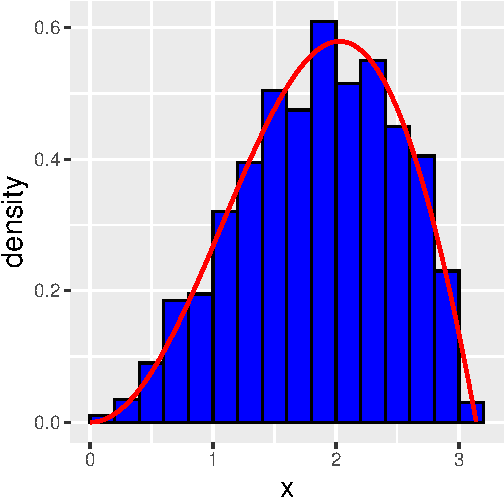
\includegraphics[keepaspectratio]{01-probability_files/figure-latex/fig-rejsamp-1.pdf}}

}

\caption{\label{fig-rejsamp}\(n = 1000\) data sampled from the
distribution \(f_X(x) = (x \sin x)/\pi\) via the rejection sampling
algorithm. We observe that our empirical distribution follows the true
distribution well.}

\end{figure}%

\begin{center}\rule{0.5\linewidth}{0.5pt}\end{center}

A primary alternative to rejection sampling is \emph{inverse transform
sampling}, in which we utilize the inverse cdf function to generate
appropriately distributed data. Inverse transform sampling is efficient
in that every proposal point is kept.

Let's suppose we are working with the pdf: \[
f_X(x) = \theta x^{\theta-1} \,,
\] where \(\theta > 0\) and \(x \in [0,1]\). The inverse cdf, as derived
in an example above, is \(F_X^{-1}(q) = q^{1/\theta}\). Inverse
transform sampling utilizes the following algorithmic steps.

\begin{enumerate}
\def\labelenumi{\arabic{enumi}.}
\tightlist
\item
  Pick the target sample size \(n\).
\item
  Sample \(n\) data with uniform weighting between 0 and 1. These are
  the cdf bounds. Call these data \(q\).
\item
  Transform the data \(q\) to be \(x = F_X^{-1}(q)\).
\end{enumerate}

In a code chunk and in Figure~\ref{fig-invsamp} we display our
inverse-transform sampling code as well as the empirical distribution of
\(n = 1000\) data sampled from our distribution (assuming
\(\theta = 3\)). We note that the code to generate our sample is
\emph{much} simpler than the code needed to perform rejection sampling!

\begin{figure}

\centering{

\pandocbounded{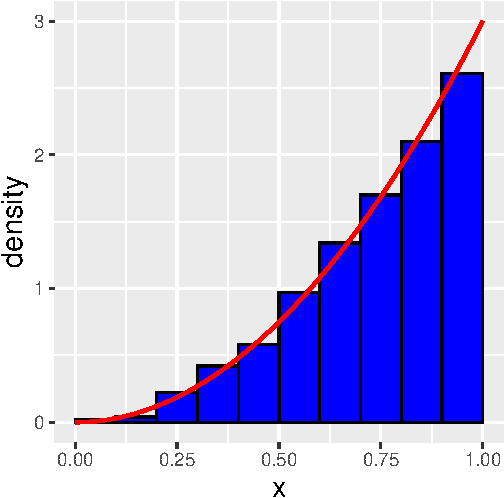
\includegraphics[keepaspectratio]{01-probability_files/figure-latex/fig-invsamp-1.pdf}}

}

\caption{\label{fig-invsamp}\(n = 1000\) data sampled from the
distribution \(f_X(x) = 3x^2\) via the inverse transform sampling
algorithm. We observe that our empirical distribution follows the true
distribution well.}

\end{figure}%

\subsection{Example}\label{example}

\subsubsection{More Inverse-Transform
Sampling}\label{more-inverse-transform-sampling}

\begin{quote}
Let's suppose that we are to sample \(n\) data from the following
distribution: \[
f_X(x) = 2(1-x) ~~~ x \in [0,1] \,.
\] Can we do this via inverse-transform sampling? The answer is yes, if
(a) we can derive the cdf \(F_X(x)\), and (b) we can invert it. Here,
\begin{align*}
F_X(x) &= \int_0^x f_V(v) dv = \int_0^x 2(1-v) dv\\
&= \left. -(1-v)^2 \right|_0^x = -(1-x)^2 - (-1) = 1 - (1-x)^2 \,.
\end{align*} To invert the cdf, we set it equal to \(q\) and solve for
\(x\): \begin{align*}
q &= 1 - (1-x)^2 \\
\Rightarrow ~~~ 1 - q &= (1-x)^2 \\
\Rightarrow ~~~ \sqrt{1 - q} &= 1-x \\
\Rightarrow ~~~ x &= 1 - \sqrt{1 - q} \,.
\end{align*} To check for the correctness of our inversion, we utilize a
code like the one in the main body of the section above and compare our
sampled data against the pdf. See Figure~\ref{fig-invsamp2}.
\end{quote}

\begin{figure}

\centering{

\pandocbounded{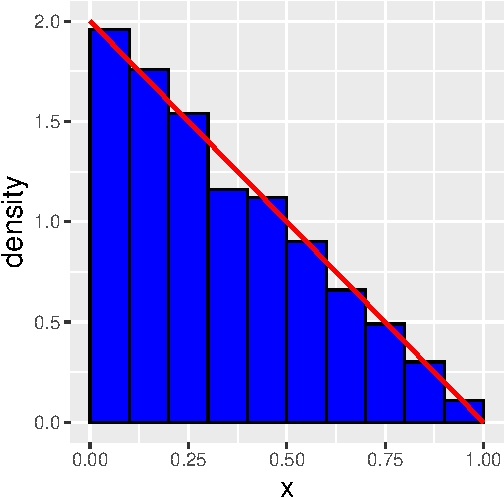
\includegraphics[keepaspectratio]{01-probability_files/figure-latex/fig-invsamp2-1.pdf}}

}

\caption{\label{fig-invsamp2}\(n = 1000\) data sampled from the
distribution \(f_X(x) = 2(1-x)\) via the inverse transform sampling
algorithm. We observe that our empirical distribution follows the true
distribution well.}

\end{figure}%

\section{Statistics and Sampling
Distributions}\label{sec-chap1statistics}

What to take away from this section:

\begin{itemize}
\item
  A \emph{statistic} is a function of observed data\ldots{}

  \begin{itemize}
  \tightlist
  \item
    \ldots hence a statistic is a random variable
  \end{itemize}
\item
  As a random variable, a statistic is sampled according to a
  \emph{sampling distribution}, which despite the name is just a
  probability distribution with an associated mass or density function.
\item
  While the ``width'' of the mass or density function associated with an
  individual datum is dubbed the standard deviation, the analogous
  quantity for a sampling distribution is called the \emph{standard
  error}.
\item
  Foreshadowing: if the observed data are sampled according to a
  probability distribution with a parameter \(\theta\), and if the value
  of \(\theta\) is unknown, then we would want to define a statistic
  that would help us infer the true value of \(\theta\), through\ldots{}

  \begin{itemize}
  \item
    point estimation;
  \item
    confidence interval estimation; or
  \item
    hypothesis testing.
  \end{itemize}
\end{itemize}

Let's say that we run an experiment in which we randomly sample many
data from some distribution \(P\): \[
\mathbf{X} = \{X_1,X_2,\ldots,X_n\} \overset{iid}{\sim} P \,.
\] The expected value for this distribution is \(E[X] = \mu\), while the
variance is \(V[X] = \sigma^2\) (assumed to be finite).

So we have data\ldots now what?

\begin{figure}

\centering{

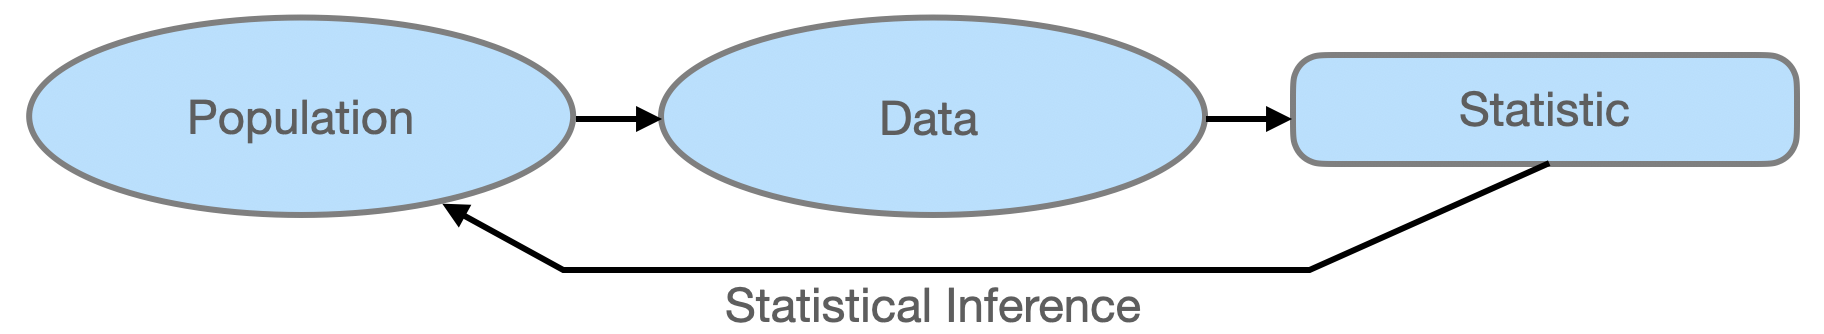
\includegraphics[width=0.75\linewidth,height=\textheight,keepaspectratio]{figures/inference_cycle.png}

}

\caption{\label{fig-cycle2}The canonical experiment-and-infer cycle. We
gather data sampled from an unknown population, assume that the
population can be represented by some family of distributions
parameterized by \(\theta\), and compute and use statistics to infer the
value(s) of \(\theta\).}

\end{figure}%

The answer, typically, is that we would use these data to \emph{infer}
the (unknown) properties of the population from which they are drawn. A
simple picture of the experiment-and-infer cycle is given in
Figure~\ref{fig-cycle2}. Notice how in this figure we use the term
``statistical inference.'' (Fitting, as it is part of the name of this
course!) This is an appropriate term to use because we utilize
statistics when trying to infer the properties of the unknown underlying
population, like its true mean \(\mu\). But this motivates a question:
what exactly is a statistic?

\subsection{Statistics}\label{sec-chap1stat}

A statistic is simply a function of the data we observe. It can be any
function of the data\(-\)e.g., \(X_1\), sin\((X_1) + \pi X_2\),
etc.\(-\)and it provides a useful means by which to summarize data
(i.e., reduce \(n\) numbers to a single number). But it should be
intuitively obvious (we would hope!) that some statistics are going to
be more informative than others: for instance, if we are trying to infer
what \(\mu\) might be, \(X_1\) is probably going to be more useful to us
than sin\((X_1) + \pi X_2\). But it may not (nay, will not) be the most
useful quantity when the sample size \(n > 1\). We could say that much
of what we do as statisticians is to pick appropriate (and optimal!)
statistics to perform inference. (Which would be true, if not for all
the data pre-processing, exploratory data analysis, coding, and
interpretation we also do as part of the job.)

What are some common statistics?

\begin{enumerate}
\def\labelenumi{\arabic{enumi}.}
\tightlist
\item
  The \emph{sample mean}: \[
  \bar{X} = \frac{1}{n} \sum_{i=1}^n X_i \,.
  \] This is always useful for inferring a population mean. Why it is
  better than, e.g., \(X_1\) when \(n > 1\) will become more clear
  below. (Foreshadowing: there are metrics we can compute that provide
  numerical assessments of the usefulness of a statistic for performing
  inference. We introduce some of these metrics in the next section.)
\item
  The \emph{sample variance}: \[
  S^2 = \frac{1}{n-1} \sum_{i=1}^n (X_1 - \bar{X})^2 \,.
  \] As we might guess, this one helps us infer population variances,
  and thus helps us make sense of the ``width'' of the pmf or pdf from
  which the data are sampled. The square root of \(S^2\) is the
  \emph{sample standard deviation}. (One might ask: why \(n-1\)?
  Metrics, again\ldots we will return to this point below when we
  discuss point estimation.)
\item
  The \emph{sample range}: \[
  R = X_{(n)} - X_{(1)} \,.
  \] Here, we introduce a notational wrinkle: \(X_{(i)}\) represents the
  \(i^{\mathrm{th}}\) \emph{smallest} datum. So \(X_{(1)}\) is the
  observed datum with the smallest value (but not necessarily the first
  one to be recorded in our experiment), and \(X_{(n)}\) is the one with
  the largest value. \(X_{(\cdot)}\) is dubbed an \emph{order statistic}
  and we will illustrate its use as we go on, beginning in
  Section~\ref{sec-chap3order}.
\item
  There are a myriad of others: the interquartile range, the median,
  etc.
\end{enumerate}

\subsection{Sampling Distributions}\label{sec-chap1sampdist}

We have stated what a statistic is: it is a function of the observed
data. But what does this imply? \textbf{It implies that statistics,
which are functions of random variables, are themselves random
variables, and thus are sampled from a pmf or pdf.} It is convention to
call the pmf or pdf associated with a given statistic the \emph{sampling
distribution}, but we are not necessarily fans of the term: it makes it
sound like something new and different, when in reality a sampling
distribution is just another pmf or pdf, with properties equivalent to
those discussed earlier in the chapter (e.g., a sampling distribution
has an expected value, a variance, etc.; see
Section~\ref{sec-chap1density} and Section~\ref{sec-chap1expected}).

As we will see in the first example below, if the statistic is a linear
function of random variables (like the sample mean), we can derive its
expected value, variance, and \emph{standard error} now given the tools
we already have at our disposal. The term standard error simply refers
to the standard deviation of a sampling distribution, i.e., \[
se[Y] = \sqrt{V[Y]} \,,
\] where \(Y\) is our statistic. Now, can we go beyond this and derive
the mathematical form of a statistic's pmf or pdf now? The short answer
is no\ldots we have not yet introduced methods for deriving the
functional forms of sampling distributions.

\begin{itemize}
\tightlist
\item
  In Section~\ref{sec-chap2methodmgf}, we will introduce
  moment-generating functions, which can help us derive sampling
  distributions for linear functions of random variables (an example of
  which is the sample mean).
\item
  In Section~\ref{sec-chap3order}, we will show how one can write down
  the pmf or pdf for order statistics (like the sample median); once the
  sampling distribution is known, then we can derive its expected value
  and variance.
\end{itemize}

(As an aside, we should mention here the \emph{empirical rule}. While
nominally about the normal distribution, we will think of it as stating
that nearly all statistics should be observed as laying within three
standard errors of their population means. For instance, as we show
below in an example, \(E[\bar{X}] = \mu\), so virtually all values of
\(\bar{X}\), as observed over repetitions of an experiment, should lie
in the range \([\mu - 3 \cdot se(\bar{X}),\mu + 3 \cdot se(\bar{X})]\),
a range that gets smaller and smaller as the sample size \(n\) goes to
infinity.)

There are, however, two paths that one could follow that allow us to
build up an empirical sampling distribution for a statistic. The first
assumes that we know (or are willing to assume) the pmf or pdf for the
individual data: we would repeatedly simulate data from the distribution
and record the values for the statistic. This builds off of the material
in Section~\ref{sec-chap1sampling}. (See the example below.) The other
is useful for situations where we do not know nor are willing to assume
the form of the pmf or pdf for the individual data\ldots this is the
\emph{bootstrap}. We discuss the bootstrap technique in
Section~\ref{sec-chap4bootstrap}.

\begin{center}\rule{0.5\linewidth}{0.5pt}\end{center}

\textbf{Many important results in statistical inference assume that we
have collected a sample of \(n\) independent and identically distributed
(or iid) random variables, so over the course of the rest of this
chapter and for the next several, we will assume that when we have
sampled two or more random variables, they will be iid random
variables.} (While the meaning of ``identically distributed'' should be
intuitively clear to the reader, ``independent'' means that the value
that we observe for one random variable will not affect the values we
might observe for another random variable. We will discuss concepts
related to simultaneously sampling values for two or more
\emph{dependent} random variables in Chapter~\ref{sec-chap6}.)

For more on sampling distributions, go to
Section~\ref{sec-chap2methodmgf}.

\subsection{Examples}\label{examples-8}

\subsubsection{Expected Value and Variance of the Sample Mean (For All
Distributions)}\label{expected-value-and-variance-of-the-sample-mean-for-all-distributions}

\begin{quote}
Given \(n\) iid data from some distribution, we can use the results from
Section~\ref{sec-chap1expected} to immediately show that \begin{align*}
E[\bar{X}] &= E\left[\frac{1}{n}\sum_{i=1}^n X_i\right] = \frac{1}{n}E\left[\sum_{i=1}^n X_i\right] = \frac{1}{n}\sum_{i=1}^n E[X_i]\\
&= \frac{1}{n}\sum_{i=1}^n \mu = \frac{1}{n} n \mu = \mu \,,
\end{align*} and \begin{align*}
V[\bar{X}] &= V\left[\frac{1}{n}\sum_{i=1}^n X_i\right] = \frac{1}{n^2} V\left[\sum_{i=1}^n X_i\right] = \frac{1}{n^2} \sum_{i=1}^n V[X_i]\\
&= \frac{1}{n^2} n \sigma^2 = \frac{\sigma^2}{n} \,.
\end{align*} The standard error for the sample mean is thus
\(\sqrt{\bar{X}} = \sigma/\sqrt{n}\). There are two important
conclusions to take away from this simple example. First, \emph{we never
state the distribution from which we sample the initial data, so this is
a general result that holds for all distributions}. Second, we see that
the width of the sampling distribution for the sample mean decreases as
we collect more and more data, as \(1/\sqrt{n}\), meaning that any
inferences that we make about the population mean will become more and
more accurate as the sample size increases.
\end{quote}

\subsubsection{Simulation: Basic
Algorithm}\label{simulation-basic-algorithm}

\begin{quote}
As we will see throughout this course, there will be times when we can
analytically derive the sampling distribution for a statistic\ldots and
times when we cannot. When we cannot, \emph{but we know or can assume
the distribution for each of the individual data}, we can fall back upon
simulations.
\end{quote}

\begin{quote}
A basic simulation algorithm, rendered in pseudocode, looks like this:
\end{quote}

\begin{verbatim}
set random number seed

set sample size and number of datasets, etc.

initialize vector(s) for storing result(s)

begin for-loop
  sample dataset
  compute statistic
  compute and store result
end for-loop

optional: process result vector 

display result
\end{verbatim}

\begin{quote}
Note the ``sample dataset'': this part of the algorithm utilizes either
previously coded data samplers (e.g., \texttt{rnorm()} in \texttt{R}),
or rejection or inverse-transform sampling as described above. Also note
that while we indicate that we would embed our data sampler within a
\texttt{for}-loop, we will often be able to leverage \texttt{R}'s
vectorization facility and its \texttt{apply()} function, which both
shortens simulation code and makes it more computationally efficient (in
terms of computation time).
\end{quote}

\begin{quote}
We will apply the basic algorithm above in examples spread throughout
the remainder of the book, starting immediately below.
\end{quote}

\subsubsection{Simulation: the Sampling Distribution of the Sample
Mean}\label{simulation-the-sampling-distribution-of-the-sample-mean}

\begin{quote}
In a previous example, we use inverse-transform sampling to sample data
from the pdf \(f_X(x) = 2(1-x)\) for \(x \in [0,1]\). Here, we extend
the \texttt{R} code so as to visualize the distribution of the sample
mean of \(n = 10\) data drawn from this distribution.
\end{quote}

\begin{figure}

\centering{

\pandocbounded{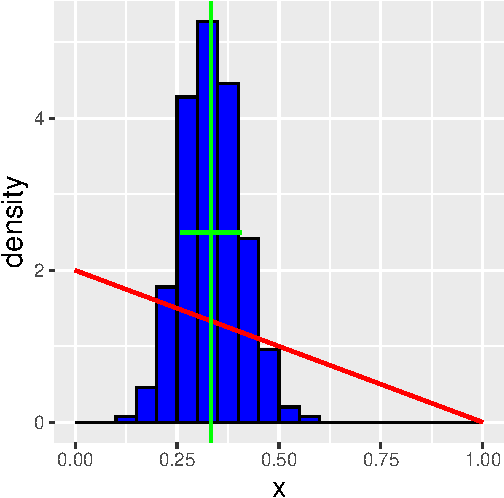
\includegraphics[keepaspectratio]{01-probability_files/figure-latex/fig-sampmean-1.pdf}}

}

\caption{\label{fig-sampmean}The empirical distribution of the sample
mean of \(n = 10\) data sampled from the distribution
\(f_X(x) = 2(1-x)\) for \(x \in [0,1]\). The red line indicates
\(f_X(x)\), while the vertical and horizontal green lines indicate
\(E[\bar{X}] = \mu = 1/3\) and the range
\([\mu-se(\bar{X}),\mu+se(\bar{X})] = [0.2588,0.4078]\). The shape of
the empirical distribution is approaching that of a normal distribution,
a result that foreshadows our discussion of the Central Limit Theorem in
Section~\ref{sec-chap2clt}.}

\end{figure}%

\begin{quote}
See Figure~\ref{fig-sampmean}. The mean of the pdf is \begin{align*}
E[X] &= \int_0^1 2x(1-x) dx = \int_0^1 2xdx - \int_0^1 2x^2dx\\
&= \left. x^2 \right|_0^1 - \left. \frac{2}{3}x^3 \right|_0^1 = 1 - \frac{2}{3} = \frac{1}{3} \,.
\end{align*} This is indicated via the green vertical line in the
figure. The variance is \begin{align*}
V[X] &= E[X^2] - (E[X])^2 \\
&= \left[ \int_0^1 2x^2dx - \int_0^1 2x^3dx \right] - \left(\frac{1}{3}\right)^2 \\
&= \left(\frac{2}{3} - \frac{1}{2}\right) - \frac{1}{9} \\
&= \frac{1}{6} - \frac{1}{9} = \frac{1}{18} \,.
\end{align*} The standard error for \(\bar{X}\) is thus \[
se(\bar{X}) = \sqrt{\frac{V[X]}{n}} = \sqrt{\frac{1}{180}} = 0.0745 \,.
\] The range from the mean minus one standard error to the mean plus one
standard error is indicated via the green horizontal line segment in the
figure.
\end{quote}

\begin{quote}
We observe that the distribution of the sample mean values matches the
expected mean and standard error well, and is \emph{definitely different
from} the distribution of the individual data values (which is shown as
the red line in the figure). The pdf for the sampling distribution looks
almost like that of a normal distribution. For now we will have to
content ourselves with only knowing the mean and the standard error of
the sampling distribution distribution, and not the mathematical form of
its pdf.
\end{quote}

\subsubsection{Simulation: the Sampling Distribution of the Sample
Median}\label{simulation-the-sampling-distribution-of-the-sample-median}

\begin{quote}
The median of a data sample is defined as the middle value of the sorted
data: if we have \(n=5\) data, for instance, the median is \(x_{(3)}\).
(Recall that the parentheses indicating that we are examining sorted
data, with \(x_{(1)}\) and \(x_{(n)}\) being the smallest and largest
observed values.) Here, we show how to simulate the distribution of a
sample median. In Section~\ref{sec-chap3order}, we show how we can
attempt to derive distributions related to sorted data mathematically.
\end{quote}

\begin{quote}
Let's assume that we draw data according to the following distribution:
\[
f_X(x) = \left\{ \begin{array}{cl} \frac{1}{\pi} x \sin x & 0 \leq x \leq \pi \\ 0 & \mbox{otherwise} \end{array} \right. \,,
\] In the code chunk below, we display the estimated mean and standard
error for the sampling distribution, while in Figure~\ref{fig-sampmed}
we show the empirical distribution of the median values.
\end{quote}

\begin{verbatim}
The empirical mean is            1.907 
\end{verbatim}

\begin{verbatim}
The empirical standard error is  0.255 
\end{verbatim}

\begin{figure}

\centering{

\pandocbounded{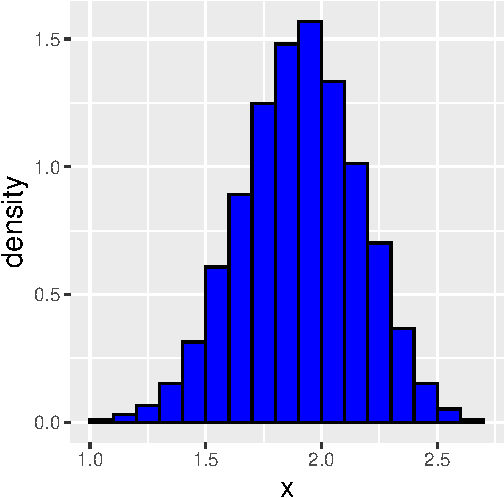
\includegraphics[keepaspectratio]{01-probability_files/figure-latex/fig-sampmed-1.pdf}}

}

\caption{\label{fig-sampmed}The empirical distribution of the sample
median for the pdf \(f_X(x) = (x \sin x)/\pi\), assuming a sample size
of \(n = 11\).}

\end{figure}%

\section{The Likelihood Function}\label{sec-chap1likelihood}

What to take away from this section:

\begin{itemize}
\item
  When we attempt to infer the true value of a distribution parameter
  \(\theta\), it can be helpful to quantify how ``likely'' a particular
  value of \(\theta\) is, given the data we observe, i.e., to define a
  \emph{likelihood function}.
\item
  Foreshadowing: a likelihood function can help us \emph{define} an
  appropriate statistic to use when performing inference.
\end{itemize}

Assume we are given iid data \(\mathbf{X} = \{X_1,\ldots,X_n\}\), with
each datum sampled from a continuous distribution
\(f_X(x \vert \theta)\). (Recall that \(\theta\) is the conventionally
used symbol for a population parameter or set of parameters. Here,
without loss of generality, we will assume that \(\theta\) represents
one parameter.) The likelihood function for the entire sample is defined
as \[
\mathcal{L}(\theta \vert \mathbf{x}) = f_X(\mathbf{x} \vert \theta) = \prod_{i=1}^n f_X(x_i \vert \theta) \,.
\] The second equality holds because the data are assumed to be iid.
Note that the same definition holds for discrete distributions, with the
notational change \(f \rightarrow p\). Additionally, recall that
\(\prod\) is the product symbol, the multiplicative analogue of the
summation symbol \(\sum\): \(\prod_{i=1}^n f_X(x_i \vert \theta) =
f_X(x_1 \vert \theta) \cdot f_X(x_2 \vert \theta) \cdot \cdots \cdot f_X(x_n \vert \theta)\).
As a last comment, we will find that we often work not with the
likelihood function itself, but with the \emph{log-likelihood} function
\(\ell(\theta \vert \mathbf{x})\); given iid data, the log-likelihood is
\[
\ell(\theta \vert \mathbf{x}) = \log \left[ \prod_{i=1}^n f_X(x_i \vert \theta) \right] = \sum_{i=1}^n \log f_X(x_i \vert \theta) \,.
\]

Let's step back for an instant here, and assume our sample size is
\(n = 1\). At first blush, it would appear that a likelihood is the same
as a probability density function, because, after all,
\(\mathcal{L}(\theta \vert x) =
f_X(x \vert \theta)\). But note what is being conditioned upon in both
functions: for the likelihood, we consider that the datum is fixed to
its observed value (i.e., \(X = x\)) and that we are free to vary the
value of \(\theta\).

To show the difference between a probability distribution and the
likelihood function, let's take a look at a simple example where we flip
a potentially unfair coin twice, with \(p\) being the probability of
observing heads in any single flip. The probability mass function for
\(X\), the random variable denoting the number of heads observed, is \[
p_X(x \vert p) = \left\{ \begin{array}{cl} 2 & p^2 \\ 1 & 2p(1-p) \\ 0 & (1-p)^2 \end{array} \right. \,.
\] The probability mass functions that arise when we set \(p\) to, e.g.,
0.3, 0.5, and 0.8 are shown in Figure~\ref{fig-pmfs}, while the
likelihood functions for each observable value of \(x\) are shown in
Figure~\ref{fig-likes}. None of the plots in Figure~\ref{fig-likes}
shows the pmf \(p_X(x \vert p)\); rather, they each show the relative
plausibility of a particular probability \(p\) given the number of
observed heads. If we observe zero (or two) heads, then a probability of
\(p=0\) (or \(p=1\)) is the most plausible value\ldots but only \(p=1\)
(or \(p=0\)) is impossible. On the other hand, when we observe one head
and one tail, the most plausible value for \(p\) is 0.5, although all
other values (save \(p=0\) and \(p=1\)) are possible as well.

\begin{figure}

\begin{minipage}[t]{0.33\linewidth}

\centering{

\pandocbounded{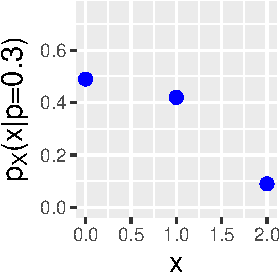
\includegraphics[keepaspectratio]{01-probability_files/figure-latex/fig-pmfs-1.pdf}}

}

\subcaption{\label{fig-pmfs-1}}

\end{minipage}%
%
\begin{minipage}[t]{0.33\linewidth}

\centering{

\pandocbounded{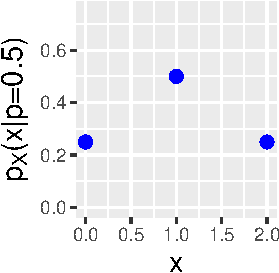
\includegraphics[keepaspectratio]{01-probability_files/figure-latex/fig-pmfs-2.pdf}}

}

\subcaption{\label{fig-pmfs-2}}

\end{minipage}%
%
\begin{minipage}[t]{0.33\linewidth}

\centering{

\pandocbounded{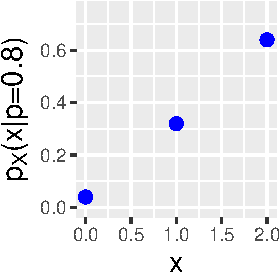
\includegraphics[keepaspectratio]{01-probability_files/figure-latex/fig-pmfs-3.pdf}}

}

\subcaption{\label{fig-pmfs-3}}

\end{minipage}%

\caption{\label{fig-pmfs}From (a) to (c), the probability mass functions
\(p_X(x \vert p)\) for probabilities \(p =\) 0.3, 0.5, and 0.8.}

\end{figure}%

\begin{figure}

\begin{minipage}[t]{0.33\linewidth}

\centering{

\pandocbounded{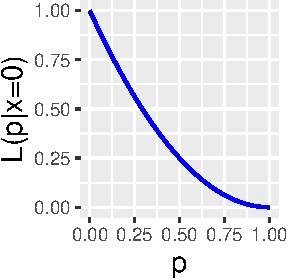
\includegraphics[keepaspectratio]{01-probability_files/figure-latex/fig-likes-1.pdf}}

}

\subcaption{\label{fig-likes-1}}

\end{minipage}%
%
\begin{minipage}[t]{0.33\linewidth}

\centering{

\pandocbounded{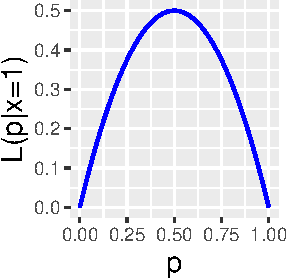
\includegraphics[keepaspectratio]{01-probability_files/figure-latex/fig-likes-2.pdf}}

}

\subcaption{\label{fig-likes-2}}

\end{minipage}%
%
\begin{minipage}[t]{0.33\linewidth}

\centering{

\pandocbounded{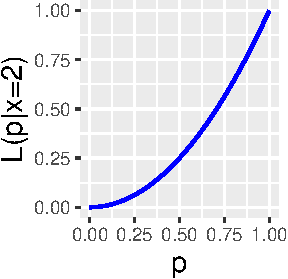
\includegraphics[keepaspectratio]{01-probability_files/figure-latex/fig-likes-3.pdf}}

}

\subcaption{\label{fig-likes-3}}

\end{minipage}%

\caption{\label{fig-likes}From (a) to (c), the likelihood function
\(\mathcal{L}(p \vert x)\) for the probability parameter \(p\) given
that we observe \(x=0\) heads, \(x=1\) head, and \(x=2\) heads,
respectively.}

\end{figure}%

One might question at this point why the likelihood function is
important, as it is indeed not a pmf or pdf. We will see below that it
is often used when trying to uncover the truth about a population: e.g.,
given a set of data, randomly sampled from some family of distributions
parameterized by \(\theta\), we can utilize the likelihood to infer, or
estimate, \(\theta\). This is because, ultimately, the likelihood is a
function of observed data, and hence \emph{the likelihood is a
statistic}.

\subsection{Examples}\label{examples-9}

\subsubsection{Examples of Likelihood Functions for IID
Data}\label{examples-of-likelihood-functions-for-iid-data}

\begin{quote}
\begin{enumerate}
\def\labelenumi{\arabic{enumi}.}
\tightlist
\item
  We are given \(n\) iid samples from \[
  f_X(x \vert \theta) = \left\{ \begin{array}{cl} \theta x^{\theta-1} & 0 \leq x \leq 1 \\ 0 & \mbox{otherwise} \end{array} \right. \,.
  \] The likelihood function is \[
  \mathcal{L}(\theta \vert \mathbf{x}) = \prod_{i=1}^n \theta x_i^{\theta-1} = \theta^n \left(\prod_{i=1}^n x_i\right)^{\theta-1} \,,
  \] while the log-likelihood function is \begin{align*}
  \ell(\theta \vert \mathbf{x}) &= \log \mathcal{L}(\theta \vert \mathbf{x}) = n \log \theta + (\theta-1) \log \prod_{i=1}^n x_i\\
  &= n \log \theta + (\theta-1) \sum_{i=1}^n \log x_i \,.
  \end{align*}
\end{enumerate}
\end{quote}

\begin{quote}
\begin{enumerate}
\def\labelenumi{\arabic{enumi}.}
\setcounter{enumi}{1}
\tightlist
\item
  We are given \(n\) iid samples from \[
  p_X(x \vert p) = \left\{ \begin{array}{cl} p & x=1 \\ 1-p & x=0 \\ 0 & \mbox{otherwise} \end{array} \right. \,.
  \] We observe \(k\) values of 1, and \(n-k\) values of 0. Thus the
  likelihood function is \[
  \mathcal{L}(p \vert \mathbf{x}) = \prod_{i=1}^n p_X(x_i \vert p) = \prod_{i=1}^k p \times \prod_{i=1}^{n-k} (1-p) = p^k(1-p)^{n-k} \,,
  \] and the log-likelihood function is \[
  \ell(p \vert \mathbf{x}) = \log \mathcal{L}(p \vert \mathbf{x}) = k \log p + (n-k) \log (1-p) \,.
  \]
\end{enumerate}
\end{quote}

\begin{quote}
\begin{enumerate}
\def\labelenumi{\arabic{enumi}.}
\setcounter{enumi}{2}
\tightlist
\item
  We are given \(n\) iid samples from the mixed distribution \[
  h_X(x \vert \theta) = \left\{ \begin{array}{cl} \frac{x}{\theta} & x \in [0,1] \\ 1-\frac{1}{2\theta} & x=2 \\ 0 & \mbox{otherwise} \end{array} \right. \,.
  \] We observe \(l\) values between 0 and 1, along with \(n-l\) values
  of 2. Let \(j\) denote the indices of those data with values between 0
  and 1, and \(k\) denote the indices of those data with value 2. The
  likelihood function is then \begin{align*}
  \mathcal{L}(\theta \vert \mathbf{x}) &= \prod_{i=1}^n h_X(x_i \vert p) = \prod_{j=1}^l \frac{x_j}{\theta} \times \prod_{k=1}^{n-l} \left(1-\frac{1}{2\theta}\right)\\
  &= \left( \frac{1}{\theta^l} \prod_{j=1}^l x_j \right) \left(1-\frac{1}{2\theta}\right)^{n-l} \,.
  \end{align*}
\end{enumerate}
\end{quote}

\subsubsection{Coding the Likelihood Function in
R}\label{coding-the-likelihood-function-in-r}

\begin{quote}
Let's code and display the likelihood function for the mixed
distribution we introduce immediately above. The first thing we will do,
however, is generate data from this distribution using inverse transform
sampling.
\end{quote}

\begin{quote}
The cdf for this distribution is \[
H_X(x \vert \theta) = \left\{ \begin{array}{cl} 0 & x < 0 \\ x^2/2\theta & 0 \leq x \leq 1 \\ 1/2\theta & 1 < x < 2 \\ 1 & x \geq 2 \end{array} \right. \,.
\] For cdf values \(q < 1/(2\theta)\), the inverse function is
\(x = \sqrt{2 \theta q}\). We thus code the inverse transform sampler as
follows\ldots{}
\end{quote}

\begin{Shaded}
\begin{Highlighting}[]
\FunctionTok{set.seed}\NormalTok{(}\DecValTok{101}\NormalTok{)}
\NormalTok{n           }\OtherTok{\textless{}{-}} \DecValTok{100}
\NormalTok{theta       }\OtherTok{\textless{}{-}} \FloatTok{1.5}
\NormalTok{q           }\OtherTok{\textless{}{-}} \FunctionTok{runif}\NormalTok{(n, }\AttributeTok{min =} \DecValTok{0}\NormalTok{, }\AttributeTok{max =} \DecValTok{1}\NormalTok{)}
\NormalTok{w           }\OtherTok{\textless{}{-}} \FunctionTok{which}\NormalTok{(q }\SpecialCharTok{\textless{}} \DecValTok{1} \SpecialCharTok{/}\NormalTok{ (}\DecValTok{2} \SpecialCharTok{*}\NormalTok{ theta))}
\NormalTok{X.sample    }\OtherTok{\textless{}{-}} \FunctionTok{rep}\NormalTok{(}\DecValTok{2}\NormalTok{, n)}
\NormalTok{X.sample[w] }\OtherTok{\textless{}{-}} \FunctionTok{sqrt}\NormalTok{(}\DecValTok{2} \SpecialCharTok{*}\NormalTok{ theta }\SpecialCharTok{*}\NormalTok{ q[w])}
\end{Highlighting}
\end{Shaded}

\begin{quote}
Given our dataset, we can compute and visualize the likelihood function
\(\mathcal{L}(\theta \vert \mathbf{x})\)\ldots but\ldots this will be
problematic. If we examine the likelihood function, we see that its
values will be (a) tiny, and (b) spread over a large dynamic range. (In
fact, for a sufficiently large dataset, the likelihood function will
have a value too small to be recordable as a floating-point number on a
computer!) Thus in practice it is often best to visualize the
log-likelihood function \(\ell(\theta \vert \mathbf{x}) =
\log \mathcal{L}(\theta \vert \mathbf{x})\) as a function of \(\theta\).
We do this below in Figure~\ref{fig-samplike}. (We will leave the
derivation of the log-likelihood as an exercise to the reader.)
\end{quote}

\begin{figure}

\centering{

\pandocbounded{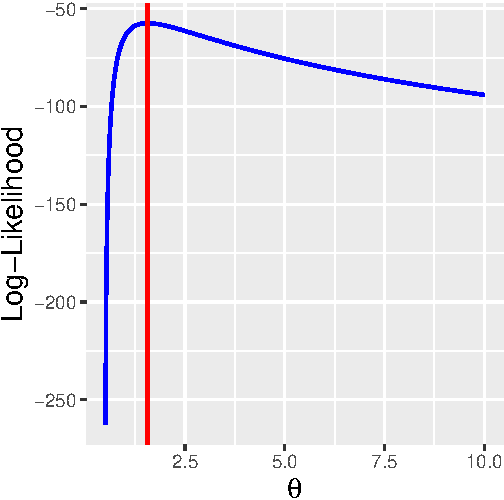
\includegraphics[keepaspectratio]{01-probability_files/figure-latex/fig-samplike-1.pdf}}

}

\caption{\label{fig-samplike}The log-likelihood function
\(\ell(\theta \vert \mathbf{x})\) for the pdf \(h_X(x \vert \theta)\)
defined in the text. The red line indicates the value of \(\theta\)
(1.56) for which \(\ell(\theta \vert \mathbf{x})\) is maximized.}

\end{figure}%

\section{Point Estimation}\label{sec-chap1point}

What to take away from this section:

\begin{itemize}
\item
  To infer the value of a probability distribution parameter \(\theta\),
  we define a statistic that is informative about \(\theta\): a
  \emph{point estimator}.
\item
  We do not need to know the sampling distribution of the defined
  statistic to carry out point estimation.
\item
  To compare competing point estimators, we evaluate their long-term
  performances via the metrics of\ldots{}

  \begin{itemize}
  \item
    \emph{bias};
  \item
    \emph{variance}; and
  \item
    \emph{mean-squared error}.
  \end{itemize}
\item
  To circumvent the guesswork that can be involved in defining an
  informative statistic, we can derive \emph{maximum likelihood
  estimates} or \emph{MLEs}.
\end{itemize}

Let's suppose we are given a sample of iid data \(\{X_1,\ldots,X_n\}\),
sampled from some distribution with mean \(E[X]\) and finite variance
\(V[X]\). As we started to discuss above, we can use functions of these
data, or statistics, to make inferences about population properties:
what are plausible values for the population mean \(\mu\)? or the
population variance \(\sigma^2\)? or, more generally, any population
parameter \(\theta\)?

In \emph{point estimation}, the statistic that we choose is an
\emph{estimator} of \(\theta\). We dub the estimate \(\hat{\theta}\):
this is a number that is our best guess for what the true value of
\(\theta\) is, given the data we have observed thus far.

Now\ldots how do we define an estimator? Well, to start, we can guess
what might be good estimators, and compare their properties. For
instance, here, let's propose two estimators for \(\mu\):
\(\hat{\mu} = X_1\) and \(\hat{\mu} = \bar{X}\). Which is better? It may
seem intuitively obvious that \(\bar{X}\) is better, because it
incorporates more data\ldots but how do we quantify ``better''?

\subsection{Estimator Bias, Variance, and Mean-Squared
Error}\label{sec-chap1mse}

In the last section, we indicated that we can assess the utility of a
statistic used as an estimator by computing metrics, quantities that
allow us to directly compare estimators. Here, we will highlight two of
them, the \emph{bias} and the \emph{variance}; later, we will highlight
others. (Recall that an estimator is a statistic, and thus it is a
random variable that is drawn from a sampling distribution with some
mean and some variance.)

\begin{enumerate}
\def\labelenumi{\arabic{enumi}.}
\tightlist
\item
  Bias: does the estimator yield the true value, \emph{on average}? In
  other words, is
  \(B[\hat{\theta}] = E[\hat{\theta}-\theta] = E[\hat{\theta}] - \theta =
  0\)? If so, we say that our estimator is \emph{unbiased}. Here, both
  estimators are unbiased: \(E[X_1-\mu] = E[X_1]-\mu = \mu-\mu = 0\),
  and \(E[\bar{X}-\mu] = E[\bar{X}] - \mu = \mu-\mu = 0\).
\item
  Variance: is the spread of values that the estimator generates from
  experiment to experiment relatively small, or relatively large?
  (Recall that it cannot be zero, due to the randomness inherent in the
  data-generating process!) Here, the first estimator has variance
  \(V[X_1] = \sigma^2\), while the second has variance
  \(V[\bar{X}] = \sigma^2/n\). (Recall that we derive the latter result
  in the previous section!) If \(n > 1\), the second estimator, with its
  smaller variance, is the better one to use. (If \(n = 1\), then
  \(\bar{X} = X_1\), so the two estimators are identical anyway.)
\end{enumerate}

See Figure~\ref{fig-biasvar} for a graphical representation of bias and
variance.

\begin{figure}

\centering{

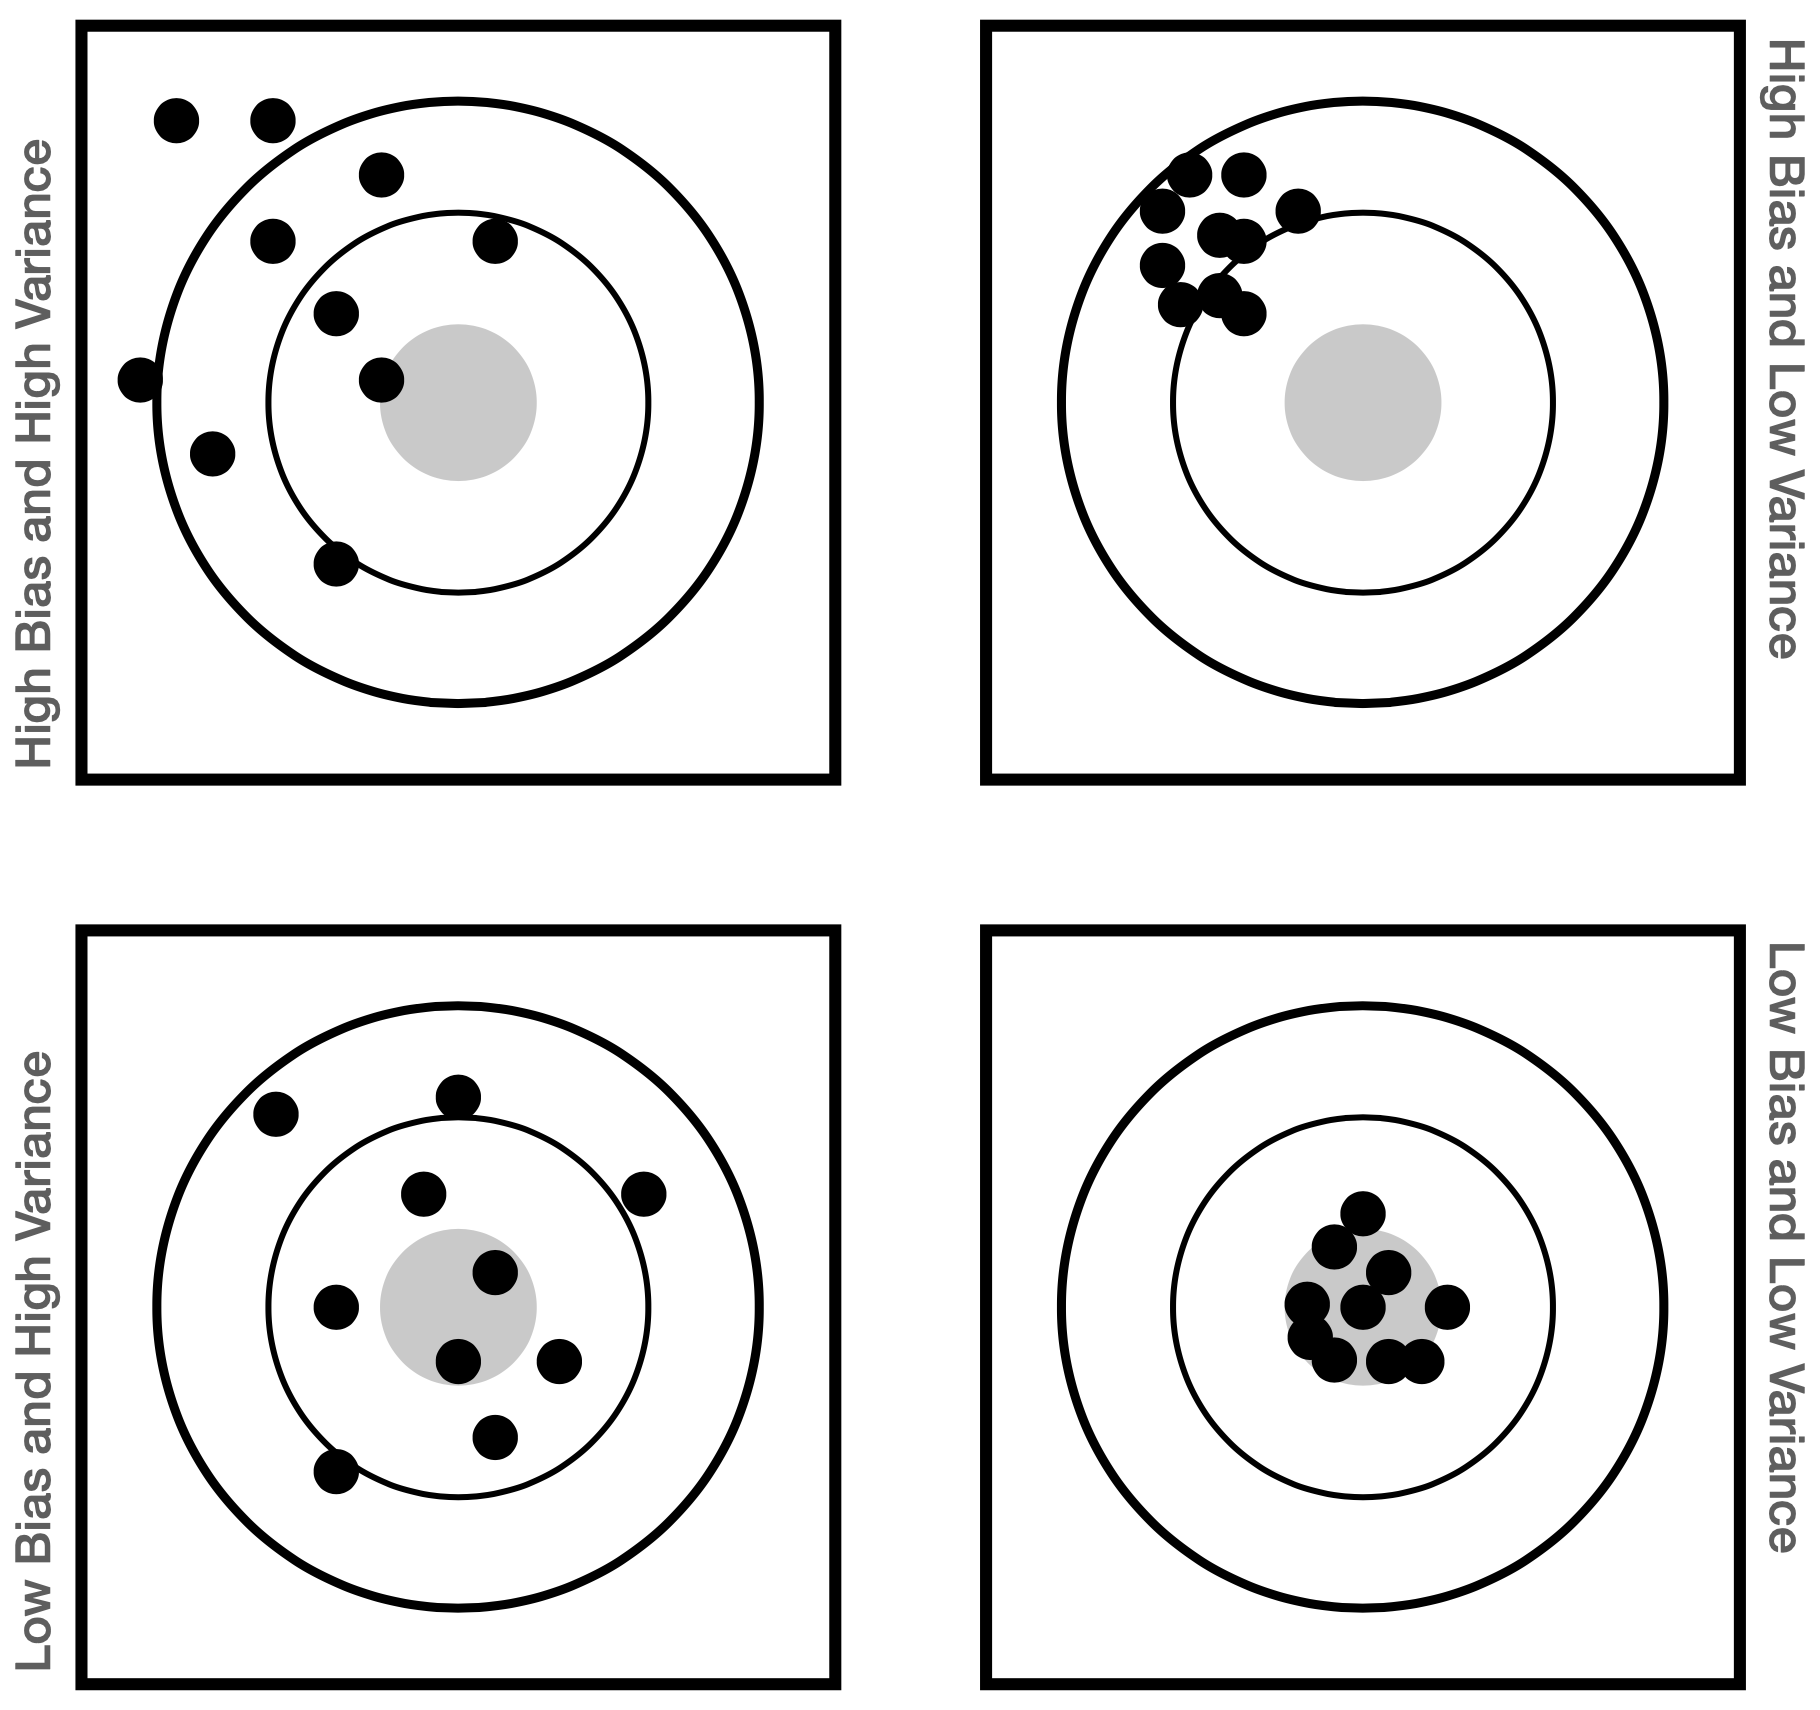
\includegraphics[width=0.6\linewidth,height=\textheight,keepaspectratio]{figures/bias_variance.png}

}

\caption{\label{fig-biasvar}A graphical representation of the concepts
of bias (how far on average an estimate is from the
truth\ldots represented here as an offset from the bullseye) and
variance (the spread of estimate values\ldots represented here as the
spatial spread of the plotted points).}

\end{figure}%

Given a choice, we generally prefer unbiased estimators with smaller
variances; however, it is theoretically possible that we might be better
off with an estimator with a small bias if it has an even lower variance
than the best unbiased one. We can start making sense of this statement
now by stating that we can combine the information about bias and
variance together into a single metric, the \emph{mean-squared error}
(or \emph{MSE}). The MSE is defined as \[
MSE[\hat{\theta}] = B[\hat{\theta}]^2 + V[\hat{\theta}] \,,
\] and smaller values are better. For \(\hat{\theta} = X_1\), the MSE is
\(0^2 + \sigma^2 = \sigma^2\), while for \(\hat{\theta} = \bar{X}\), the
MSE is \(0^2 + \sigma^2/n = \sigma^2/n\); \(\bar{X}\) is still the
better estimator.

The mean-squared error is an example of a \emph{risk function}, a
quantity which in turn is the expected value of a \emph{loss function}.
For the MSE, the associated loss function is the ``squared error loss,''
or \((\theta - \hat{\theta})^2\), and the goal of estimation is to
minimize this value. We note that there are a myriad of other loss
functions that we could utilize in point estimation, but any discussion
of these is beyond the scope of the present book.

\subsection{Maximum Likelihood Estimation}\label{sec-chap1mle}

At this point, one might be thinking that guessing estimators would be a
sub-optimal approach. And one would be correct. Over the remainder of
the book, we introduce different algorithmic approaches for defining
estimators with (presumably) good properties. Here we examine a first
one: \emph{maximum likelihood estimation} (or \emph{MLE}).

Above, in the section introducing the likelihood, we discussed how the
likelihood function \(\mathcal{L}(\theta \vert \mathbf{x})\)
encapsulates the relative plausibilities of different values of
\(\theta\) given the data that are observed. Maximum likelihood
estimation takes this idea to its natural conclusion: the most plausible
value of \(\theta\), the one that maximizes the likelihood function,
\emph{is} indeed a good way to estimate the true value of \(\theta\).
Assuming that the likelihood function achieves a maximum away from
\(\theta_{\mathrm{lo}}\) and \(\theta_{\mathrm{hi}}\), the parameter
bounds, then the steps to find \(\hat{\theta}_{MLE}\) involve
straightforward calculus, albeit with a simplifying twist:

\begin{enumerate}
\def\labelenumi{\arabic{enumi}.}
\tightlist
\item
  Write down the likelihood function:
  \(\mathcal{L}(\theta \vert \mathbf{x}) = \prod_{i=1}^n f_X(x_i \vert \theta)\).
\item
  Take the natural logarithm of \(\mathcal{L}\):
  \(\ell(\theta \vert \mathbf{x}) = \log \mathcal{L}(\theta \vert \mathbf{x}) = \sum_{i=1}^n \log f_X(x_i \vert \theta)\).
\item
  Compute the first derivative of \(\ell(\theta \vert \mathbf{x})\) with
  respect to \(\theta\). If \(\theta\) represents more than one
  parameter, take the first \emph{partial} derivative with respect to
  the parameter of interest.
\item
  Set \(\ell'(\theta \vert \mathbf{x}) = 0\).
\item
  Solve for \(\theta\). The solution is \(\hat{\theta}_{MLE}\), assuming
  that the second derivative of \(\ell(\theta \vert \mathbf{x})\) is
  negative (i.e., concave down); otherwise, we have actually found a
  local \emph{minimum} of the likelihood function.
\end{enumerate}

Note that the ``simplifying twist'' is transforming the likelihood
\(\mathcal{L}(\theta \vert \mathbf{x})\) to the log-likelihood
\(\ell(\theta \vert \mathbf{x})\); differentiating the latter is often,
if not always, easier than differentiating the former. But even if we
skip step 2 and compute the first derivative of
\(\mathcal{L}(\theta \vert \mathbf{x})\) directly, we will eventually
get the same expression for \(\hat{\theta}_{MLE}\).

For more on point estimation, go to Section~\ref{sec-chap2point}.

\subsection{Examples}\label{examples-10}

\subsubsection{Comparing Two Estimators}\label{comparing-two-estimators}

\begin{quote}
Let's assume that we are given \(n\) iid data sampled from the following
pdf: \[
f_X(x) = \frac{1}{\theta} 
\] for \(0 \leq x \leq \theta\), with \(\theta\) unknown. The expected
value and variance of this distribution are \(\mu = E[X] = \theta/2\)
and \(\sigma^2 = V[X] =
\theta^2/12\), respectively. We propose two estimators for \(\theta\):
\(2\bar{X}\), and \(X_1+X_2\). Which is better? Intuitively, we know the
answer, but can we quantify it, i.e., can we determine which of the two
estimators has a smaller mean-squared error?
\end{quote}

\begin{quote}
For \(\hat{\theta} = 2\bar{X}\), the expected value is \[
E[2\bar{X}] = 2E[\bar{X}] = 2\mu = \theta \,,
\] and thus we can see that \(2\bar{X}\) is unbiased. (Here, we utilize
the general result that \(E[\bar{X}] = \mu\).) Thus the MSE will simply
be the variance of this estimator: \[
MSE[\hat{\theta}] = V[2\bar{X}] = 4V[\bar{X}] = 4\frac{\sigma^2}{n} = \frac{\theta^2}{3n} \,.
\] (Here, we utilize the general result that
\(V[\bar{X}] = \frac{\sigma^2}{n}\).)
\end{quote}

\begin{quote}
For \(\hat{\theta} = X_1 + X_2\), the expected value is \[
E[X_1+X_2] = E[X_1] + E[X_2] = \frac{\theta}{2} + \frac{\theta}{2} = \theta \,.
\] The estimator is unbiased. The MSE is thus \[
MSE[\hat{\theta}] = V[X_1+X_2] = V[X_1] + V[X_2] = \frac{\theta^2}{12} + \frac{\theta^2}{12} = \frac{\theta^2}{6} \,.
\]
\end{quote}

\begin{quote}
Compare the two MSE expressions, keeping in mind that the second one is
meaningless if \(n=1\). For \(n=2\) the MSEs are equivalent, which makes
sense since the estimators themselves are equivalent. If \(n > 2\), then
the MSE for \(\hat{\theta} = 2\bar{X}\), is smaller, and it will
continue getting smaller as \(n\) increases, unlike the MSE for
\(\hat{\theta} = X_1 + X_2\).
\end{quote}

\subsubsection{Maximum Likelihood Estimate of Population
Parameter}\label{maximum-likelihood-estimate-of-population-parameter}

\begin{quote}
Let's assume that we are given \(n\) iid data sampled from the following
pdf: \[
f_X(x) = \frac{1}{\theta}\exp({-x/\theta}) \,,
\] with \(x \geq 0\) and \(\theta > 0\). (To be clear: in real-life
situations, we do not know the form of the pmf or pdf from which the
data are sampled! We \emph{assume} a family of distributions, then
estimate the value of the population parameter of interest.) For this
distribution, \(E[X] = \theta\) and \(V[X] = \theta^2\). The likelihood
function is \[
\mathcal{L}(\theta \vert \mathbf{x}) = \prod_{i=1}^n \frac{1}{\theta}\exp\left(-\frac{x_i}{\theta}\right) = \frac{1}{\theta^n} \prod_{i=1}^n \exp\left(-\frac{x_i}{\theta}\right) = \frac{1}{\theta^n} \exp\left(-\frac{1}{\theta}\sum_{i=1}^n x_i\right) \,,
\] and the log-likelihood is \[
\ell(\theta \vert \mathbf{x}) = \log \left[ \frac{1}{\theta^n} \exp\left(-\frac{1}{\theta}\sum_{i=1}^n x_i\right) \right] = -n \log \theta - \frac{1}{\theta} \sum_{i=1}^n x_i \,.
\] The next step in determining \(\hat{\theta}_{MLE}\) is to take the
first derivative with respect to \(\theta\), \[
\ell'(\theta \vert \mathbf{x}) = \frac{d}{d\theta} \ell(\theta \vert \mathbf{x}) = -\frac{n}{\theta} + \frac{1}{\theta^2} \sum_{i=1}^n x_i \,,
\] and set the result equal to zero: \[ 
-\frac{n}{\theta} + \frac{1}{\theta^2} \sum_{i=1}^n x_i = 0 = -n + \frac{1}{\theta} \sum_{i=1}^n x_i \,.
\] Solving for \(\theta\), we get \[
\hat{\theta}_{MLE} = \frac{1}{n} \sum_{i=1}^n X_i = \bar{X} \,.
\] When we switched from solving for the generic quantity \(\theta\) to
solving for an estimator, which is a function of random variables, we
switched from using the lower-case generic variable \(x\) to using an
upper-case-denoted random variable \(X\).
\end{quote}

\begin{quote}
(Note that we should check to see whether the second derivative is
negative at the extremum, indicating that \(\hat{\theta}_{MLE}\) is
located at a local maximum of the likelihood function rather than a
minimum. So: \[
\ell''(\theta \vert \mathbf{x}) = \frac{d}{d\theta} \ell'(\theta \vert \mathbf{x}) = \frac{n}{\theta^2} - \frac{2}{\theta^3} \sum_{i=1}^n x_i = \frac{n}{\theta^2} \left( 1 - \frac{2n}{\theta}\bar{x} \right)\,.
\] Let's plug in \(\theta = \hat{\theta}_{MLE} = \bar{x}\): \[
\ell''(\hat{\theta}_{MLE} \vert \mathbf{x}) = \frac{n}{\bar{x}^2} \left( 1 - 2n \right) \,.
\] We know that \(n\) is positive and \(\geq 1\) and that
\(\bar{x} > 0\), so indeed
\(\ell''(\hat{\theta}_{MLE} \vert \mathbf{x}) < 0\) and thus we have
detected a maximum of the likelihood function.)
\end{quote}

\begin{quote}
Now, is this estimate biased? We know from results shown above that
\(E[\bar{X}] = \theta\), thus
\(B[\hat{\theta}_{MLE}] = E[\hat{\theta}_{MLE}] - \theta
= \theta - \theta = 0\) and thus the estimator is unbiased. We also know
that \(V[\bar{X}] = \sigma^2/n = \theta^2/n\). The question, to be
answered in Section~\ref{sec-chap2crlb}, is whether we can possibly find
an estimator with a lower variance via some other estimation
approach\ldots or if this indeed the best that we can do.
\end{quote}

\begin{quote}
Now, when we solve for, e.g., \(\hat{\theta}_{MLE}\), we can solve for
other quantities as well\ldots it is just algebra. Meaning, for
instance, that if we want to estimate \(\hat{\theta}_{MLE}^2\) for
whatever reason, we can just square both sides in the solution above: \[
(\hat{\theta}_{MLE})^2 = (\bar{X})^2 ~~\Rightarrow~~ \hat{\theta}_{MLE}^2 = \bar{X}^2 \,.
\] (This is a manifestation of the so-called \emph{invariance property}
of the MLE.) Now, is \emph{this} a biased estimator for \(\theta^2\)? We
can utilize the shortcut formula for computing variance to find that \[
E[\bar{X}^2] = V[\bar{X}] + (E[\bar{X}])^2 = \frac{\sigma^2}{n} + \mu^2 = \frac{\theta^2}{n} + \theta^2 = \theta^2 \left( 1 + \frac{1}{n} \right) \neq \theta^2 \,.
\] This estimator \emph{is} biased\ldots but the bias goes away as the
sample size \(n\) increases. That means that we would call this
estimator \emph{asymptotically unbiased}, i.e., it is unbiased when the
sample size is infinite. We note here that maximum likelihood estimates
are always either unbiased or asymptotically unbiased.
\end{quote}

\subsubsection{Simulation: Sampling Distribution of Maximum Likelihood
Estimates}\label{simulation-sampling-distribution-of-maximum-likelihood-estimates}

\begin{quote}
To drive home the point that maximum likelihood estimates are random
variables, we simulate the process of estimating \(\theta\) for the pdf
\(f_X(x) = \theta x^{\theta-1}\), where \(x \in [0,1]\).
\end{quote}

\begin{quote}
Let's write down the (log-)likelihood: \begin{align*}
\mathcal{L}(\theta \vert \mathbf{x}) &= \prod_{i=1}^n \theta x_i^{\theta-1} \\
&= \theta^n \left( \prod_{i=1}^n x_i \right)^{\theta - 1} \\
\Rightarrow ~ \ell(\theta \vert \mathbf{x}) &= n \log \theta + (\theta-1)\log \left( \prod_{i=1}^n x_i \right) \\
&= n \log \theta + (\theta-1) \sum_{i=1}^n \log x_i \,,
\end{align*} and solve for the MLE: \[
\frac{d}{d\theta} \ell(\theta \vert \mathbf{x}) = \frac{n}{\theta} + \sum_{i=1}^n \log x_i ~ \Rightarrow ~ \hat{\theta}_{MLE} = -\frac{n}{\sum_{i=1}^n \log x_i} \,.
\] Given this expression, we can now determine the empirical
distribution. See Figure~\ref{fig-empmle}. We observe immediately that
the distribution is right-skewed. (As we will see in
Section~\ref{sec-chap2mle}, as \(n \rightarrow \infty\), the empirical
distribution will tend more and more to a bell-curve-like shape.)
\end{quote}

\begin{verbatim}
The empirical mean is                2.317 
\end{verbatim}

\begin{verbatim}
The empirical standard deviation is  0.377 
\end{verbatim}

\begin{figure}

\centering{

\pandocbounded{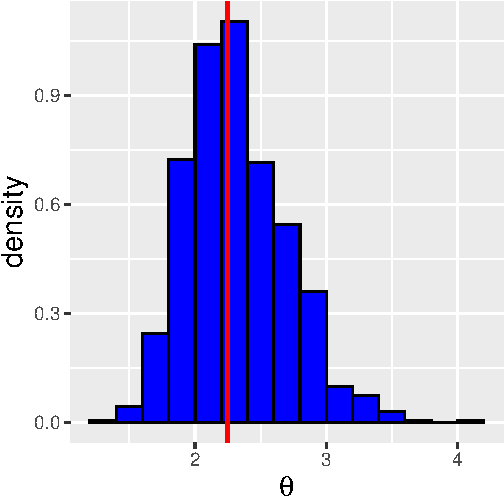
\includegraphics[keepaspectratio]{01-probability_files/figure-latex/fig-empmle-1.pdf}}

}

\caption{\label{fig-empmle}The empirical distribution of maximum
likelihood estimates for \(\theta\) for the distribution
\(f_X(x) = \theta x^{\theta-1}\) (\(x \in [0,1]\)) with
\(\theta = 2.25\) (red line) and \(n = 40\).}

\end{figure}%

\section{Statistical Inference with Sampling
Distributions}\label{sec-chap1inference}

What to take away from this section:

\begin{itemize}
\tightlist
\item
  How the sampling distribution of a defined statistic can help us infer
  plausible ranges for a distribution parameter \(\theta\), or allow us
  to test whether a proposed value for \(\theta\) is plausible.
\end{itemize}

A fundamental issue with point estimation is that, e.g., it does not
provide a notion of how uncertain the estimate is. By this, we do not
mean the standard error of the sampling distribution for the statistic
we use when making the estimate (which is a quantity that we can
derive), but rather how large (or small) is the range of plausible
values of \(\theta\) given the observed value of the statistic? Point
estimation also does not allow us to answer the question of ``is a
particular hypothesized value of \(\theta\) plausible given what we
observe?'' We can resolve the first issue by computing a
\emph{confidence interval} for \(\theta\), and the second via
\emph{hypothesis testing}. We discuss each of these concepts in turn in
the next two sections. Before doing so, however, we will show how the
construction of confidence intervals and the performance of hypothesis
tests both boil down to performing a root-finding exercise in which we
work directly with a sampling distribution.

Let's posit a simple situation in which we sample a single datum
according to the following probability density function: \[
f_X(x \vert \theta) = \frac{1}{2} ~~~ x \in [\theta-1,\theta+1]
\] Our statistic is thus \(Y = X\), and the sampling distribution
\(f_Y(y \vert \theta)\) is equivalent to \(f_X(x \vert \theta)\).
(Beginning in Chapter~\ref{sec-chap2}, we will discuss how to derive
sampling distributions for statistics computed from \(n\) independent
and identically distributed {[}iid{]} random variables, and begin to
work with more typically seen statistics like \(\bar{X}\).) We can alter
the shape and/or location of the sampling distribution by changing the
value(s) of \(\theta\). In Figure~\ref{fig-samppdf}, we show how the pdf
moves with \(\theta\); as \(\theta\) changes from 2.8 to 5.2, the pdf
shifts (smoothly) from the location indicated by the red lines to that
indicated by the blue lines. Now, let's assume that the green line in
the figure, at value \(y_{\mathrm{obs}} = 3.4\), is the statistic value
that we actually observe. What can we conclude right away, on the basis
of this figure? We can conclude that this observed value is
\emph{plausible} if \(\theta = 2.8\), but \emph{implausible} if
\(\theta = 5.2\). In other words, 2.8 is an ``acceptable'' value for
\(\theta\), but 5.2 is not.

\begin{figure}

\centering{

\pandocbounded{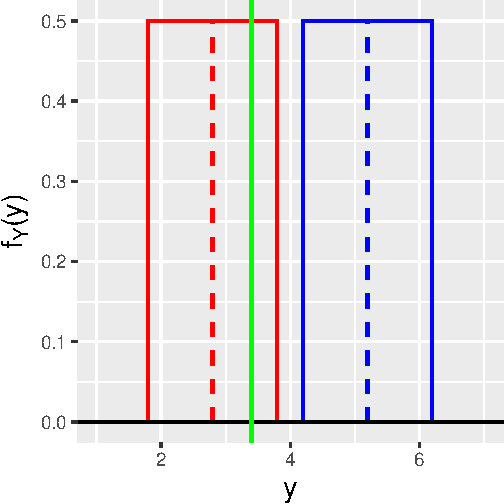
\includegraphics[keepaspectratio]{01-probability_files/figure-latex/fig-samppdf-1.pdf}}

}

\caption{\label{fig-samppdf}An illustration of how a sampling
distribution pdf can move as the distribution parameter is changed.
Here, \(f_Y(y) = 1/2\) for \(y \in [\theta-1,\theta+1]\); the red lines
represent the pdf for \(\theta = 2.8\) and the blue lines represents the
pdf for \(\theta=5.2\). The green vertical line represents the observed
value of the statistic \(Y\): \(y_{\mathrm{obs}} = 3.4\).}

\end{figure}%

To determine the range of plausible values of \(\theta\), given the data
we observe, we can invert each of the following cdf-based equations: \[
F_Y(y_{\mathrm{obs}} \vert \theta) = 0 ~~~\mbox{and}~~~ F_Y(y_{\mathrm{obs}} \vert \theta) = 1 \,,
\] where \(F_Y(y_{\mathrm{obs}} \vert \theta)\) is the cdf of \(Y\)
evaluated at the coordinate \(y_{\mathrm{obs}}\). The cdf is \[
F_Y(y \vert \theta) = \int_{\theta-1}^y \frac{dx}{2} = \left. \frac{x}{2} \right|_{\theta-1}^y = \frac12(y-\theta+1) \,,
\] and thus the solutions to the two equations above are \[
\theta = y_{\mathrm{obs}}+1 ~~~\mbox{and}~~~ \theta = y_{\mathrm{obs}}-1 \,.
\] Our ``plausible interval'' is
\([y_{\mathrm{obs}}-1,y_{\mathrm{obs}}+1]\), or here, \([2.4,4.4]\).

However, there is an issue with our initial approach: it only provides
an informative interval for \(\theta\) if the pdf for \(Y\) has a
finite, bounded domain. If, for instance, the pdf for \(Y\) has the
domain \((-\infty,\infty)\), and \(\theta\) represented the mean of
\(Y\)'s sampling distribution, then our plausible interval for
\(\theta\) would also be \((-\infty,\infty)\). To generalize the
workflow, we first combine the two equations above into the single
equation \[
F_Y(y_{\mathrm{obs}} \vert \theta) - q = 0 \,,
\] where \(q \in [0,1]\) is an appropriately chosen distribution
quantile. (Above, we set \(q\) to 0 and to 1.) Appealing to convention,
for now, we will set \(q\) to either \(\alpha/2\) or \(1 - \alpha/2\),
where \(\alpha\) is typically set to 0.05. (This convention is grounded
in the idea that we wish balance the tradeoff between interval
length\(-\)shorter intervals are ``better''\(-\)and interval
coverage\(-\)smaller values of \(\alpha\) are better.)

\begin{figure}

\begin{minipage}[t]{0.50\linewidth}

\centering{

\pandocbounded{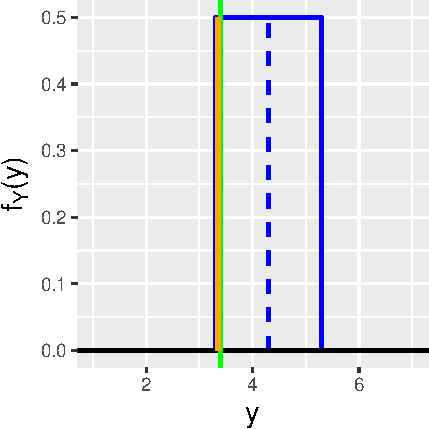
\includegraphics[keepaspectratio]{01-probability_files/figure-latex/fig-sampci-1.pdf}}

}

\subcaption{\label{fig-sampci-1}}

\end{minipage}%
%
\begin{minipage}[t]{0.50\linewidth}

\centering{

\pandocbounded{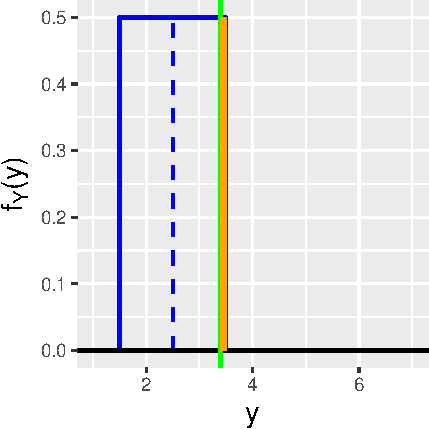
\includegraphics[keepaspectratio]{01-probability_files/figure-latex/fig-sampci-2.pdf}}

}

\subcaption{\label{fig-sampci-2}}

\end{minipage}%

\caption{\label{fig-sampci}Given the setting defined in
Figure~\ref{fig-samppdf}, we can ask (a) for what value of \(\theta\) is
the area under \(f_Y(y)\) to the left of \(y_{\mathrm{obs}}\) equal to
\(\alpha/2\), and (b) for what other value of \(\theta\) is the area
under \(f_Y(y)\) to the right of \(y_{\mathrm{obs}}\) equal to
\(\alpha/2\)? These two values comprise a two-sided confidence interval.
Here, \(\alpha = 0.1\). For \(y_{\mathrm{obs}} = 3.4\), the two values
of \(\theta\) are 2.5 and 4.3.}

\end{figure}%

(See Figure~\ref{fig-sampci}.) And here we come back to the notion that
this is a ``root-finding exercise.'' One bound is found by solving \[
F_Y(y_{\mathrm{obs}} \vert \theta) - \frac{\alpha}{2} = 0 \,,
\] and calling the solution \(\hat{\theta}_U\). As we can see in the
left panel of the figure, \(\hat{\theta}_U\) represents the \emph{upper
bound} on \(\theta\). (See Figure~\ref{fig-sampci2} for an alternative
illustration showing what is happening when we are ``finding roots.'')
The other bound, \(\hat{\theta}_L\), is found by solving \[
F_Y(y_{\mathrm{obs}} \vert \theta) - \left(1-\frac{\alpha}{2}\right) = 0 \,.
\] We will note here that in relatively rare circumstances, we can solve
for \(\hat{\theta}_L\) and \(\hat{\theta}_U\) by hand, but as we will
see later, we can always solve for these quantities numerically using,
e.g., \texttt{R}'s \texttt{uniroot()} function.

\begin{figure}

\begin{minipage}[t]{0.50\linewidth}

\centering{

\pandocbounded{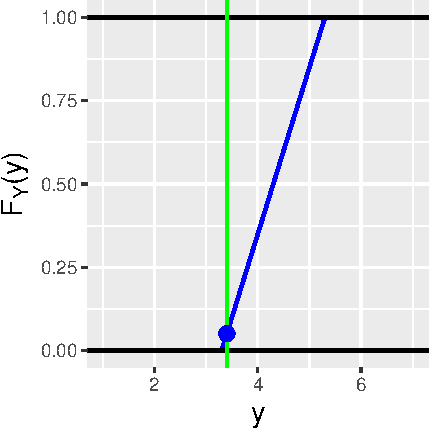
\includegraphics[keepaspectratio]{01-probability_files/figure-latex/fig-sampci2-1.pdf}}

}

\subcaption{\label{fig-sampci2-1}}

\end{minipage}%
%
\begin{minipage}[t]{0.50\linewidth}

\centering{

\pandocbounded{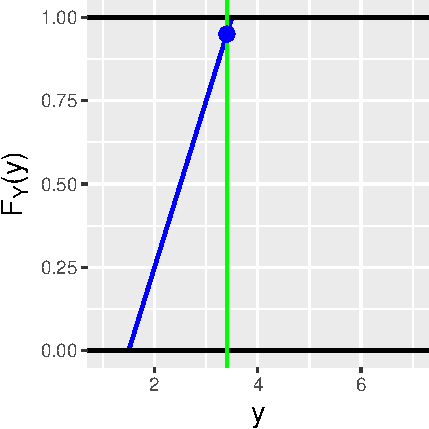
\includegraphics[keepaspectratio]{01-probability_files/figure-latex/fig-sampci2-2.pdf}}

}

\subcaption{\label{fig-sampci2-2}}

\end{minipage}%

\caption{\label{fig-sampci2}In this alternative illustration to
Figure~\ref{fig-sampci}, we show how the interval bounds are found by
changing the value of \(\theta\) until the cumulative distribution
function \(F_Y(y_{\mathrm{obs}} \vert \theta) = \alpha/2 = 0.05\) (on
the left, for \(\theta = 4.3\), given that \(y_{\mathrm{obs}} = 3.4\))
and until \(F_Y(y_{\mathrm{obs}} \vert \theta) = \alpha/2 = 0.95\) (on
the right, for \(\theta = 2.5\)).}

\end{figure}%

Now, what about hypothesis testing? As we will see below, in a
hypothesis test, we adopt a \emph{null hypothesis}
(\(\theta = \theta_o\)) and an \emph{alternative hypothesis} (e.g.,
\(\theta \neq \theta_o\)), and we combine this information with
\(y_{\mathrm{obs}}\) to determine whether the null hypothesis is viable
(in which case we ``fail to reject the null'') or not (in which case we
``reject the null''). For a two-tail test, we would determine the
boundaries of the so-called \emph{rejection region} by finding the roots
\(y_{\mathrm{RR,lo}}\) and \(y_{\mathrm{RR,hi}}\) for each of the
following equations \begin{align*}
F_Y(y_{\mathrm{RR,lo}} \vert \theta_o) - \frac{\alpha}{2} &= 0 ~~\Rightarrow~~ y_{\mathrm{RR,lo}} = F_Y^{-1}(\alpha/2 \vert \theta_o) \\
F_Y(y_{\mathrm{RR,hi}} \vert \theta_o) - \left(1-\frac{\alpha}{2}\right) &= 0 ~~\Rightarrow~~ y_{\mathrm{RR,hi}} = F_Y^{-1}(1-\alpha/2 \vert \theta_o)\,,
\end{align*} where \(F_Y^{-1}(\cdot)\) is the inverse cdf function for
\(Y\)'s sampling distribution. Here, if
\(y_{\mathrm{obs}} < y_{\mathrm{RR,lo}}\) or
\(y_{\mathrm{obs}} > y_{\mathrm{RR,hi}}\), we would reject the null,
i.e., we would deem the stated value \(\theta_o\) to be implausible
implausible. Note how the equations above are the same ones we use when
constructing confidence intervals; here we fix \(\theta = \theta_o\) (as
opposed to solving for \(\theta\)) and we solve for \(y\) (as opposed to
fixing \(y = y_{\mathrm{obs}}\)). As is the case for confidence
intervals, sometimes we can find the roots by hand, but if not, we can
often find them by using off-the-shelf inverse cdf codes like
\texttt{R}'s \texttt{qnorm()} (if the sampling distribution is a normal
distribution), etc.

\begin{center}\rule{0.5\linewidth}{0.5pt}\end{center}

An important message to take away from this section is that confidences
interval estimation and hypothesis testing both involve the same
fundamental root-finding exercise: they only differ in what values are
fixed and what values we are solving for!

\section{Confidence Intervals}\label{sec-chap1confidence}

What to take away from this section:

\begin{itemize}
\item
  The sampling distribution of a defined statistic can help us construct
  a \emph{confidence interval} for a distribution parameter \(\theta\),
  that has a long-term probabilistic guarantee of overlapping, or
  \emph{covering}, \(\theta\)'s true value.
\item
  The fundamental equation underlying interval estimation is \[
  F_Y(y_{\mathrm{obs}} \vert \theta) - q = 0 \,,
  \] which we solve for \(\theta\); \(Y\) is our defined statistic,
  \(y_{\mathrm{obs}}\) is the observed value of \(Y\), and \(q\) is an
  appropriately chosen distribution quantile.
\end{itemize}

\emph{Interval estimation} is a mechanism to determine a range of
possible values for a distribution parameter \(\theta\) that overlaps
the true but unknown value with some stated probability. A two-sided
interval estimate, or \emph{confidence interval}, has the form \[
P\left( \hat{\theta}_L \leq \theta \leq \hat{\theta}_U \right) = 1 - \alpha \,,
\] where \(1 - \alpha\) is the user-set \emph{confidence coefficient},
which typically has the value 0.95 (or \(\alpha = 0.05\)). (Technically,
the confidence coefficient is the infimum (i.e., the minimum value) of
the coverage probabilities for a particular interval estimator. This
nuance is not important if we utilize the general root-finding algorithm
laid out in the last section to determine interval bounds. We will
return to this point in an example in
Section~\ref{sec-chap5confidence}.) One can also define one-sided
intervals: \[
P\left( \hat{\theta}_L \leq \theta \right) = 1 - \alpha ~~\mbox{and}~~ P\left( \theta \leq \hat{\theta}_U \right) = 1 - \alpha \,.
\]

It is important for us to interpret an interval estimate correctly:

\begin{enumerate}
\def\labelenumi{\arabic{enumi}.}
\tightlist
\item
  it is a \emph{random interval}, meaning that if we re-do the
  data-generating experiment, the interval will change; and
\item
  we state that \emph{the probability that, e.g., the two-sided interval
  estimate \([\hat{\theta}_L,\hat{\theta}_U]\) will overlap \(\theta\)
  is \(1 - \alpha\)}.
\end{enumerate}

In particular, one does not say ``the probability that \(\theta\) lies
in the stated interval is \(1-\alpha\).'' \(\theta\) is a population
quantity, and thus we cannot make probabilistic statements about it. It
has the (unknown) value it has. Stated another way, in reference to
point 2: the probability of \(1 - \alpha\) refers to the reliability of
the estimation procedure and not to any one specific interval. For
instance, if we compute an interval of {[}1,2{]} and then re-do the
experiment and compute an interval of {[}2.5,3.5{]}, and if we say there
is a 95\% chance that \(\theta\) is in {[}1,2{]} and a 95\% chance it is
in {[}2.5,3.5{]}, then there must be a 190\% chance it is in either. A
computed interval either overlaps the true value, or it does not; it is
no longer a matter of probability. See Figure~\ref{fig-overlap}.

\begin{figure}

\centering{

\pandocbounded{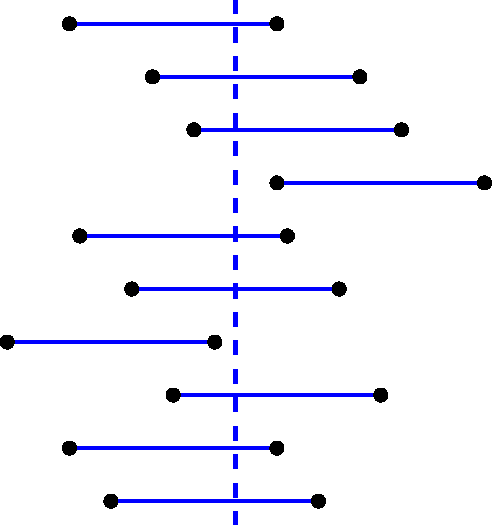
\includegraphics[keepaspectratio]{01-probability_files/figure-latex/fig-overlap-1.pdf}}

}

\caption{\label{fig-overlap}Schematic illustration of ten confidence
intervals constructed given ten separate independent datasets sampled
from the same underlying population. We indicate the true parameter
value \(\theta\) with the vertical dashed line. Counting from the
bottom, we observe that the fourth and seventh intervals do not overlap
the true value; if we were to claim that the probability that \(\theta\)
lies within each interval is, e.g., 0.95, then the probability that
\(\theta\) lies in either the fourth or seventh interval is
1.9\ldots which is clearly wrong. Thus the proper interpretation would
be that 95 percent of evaluated intervals overlap the true value.}

\end{figure}%

As laid out in the last section above, to determine a confidence
interval bound, one would determine the root of the following equation:
\begin{align*}
F_Y(y_{\mathrm{obs}} \vert \theta) - q &= 0 \,.
\end{align*} There is a very important nuance here, however, that we
ignored in the last section, which is that it is not guaranteed that the
value of the statistic \(Y\) that we adopt to construct the interval
increases as \(\theta\) increases. What that means here is that if,
e.g., \(q = \alpha/2\), then the root \(\hat{\theta}\) might represent
an upper bound on \(\theta\)\ldots but it might represent a lower bound
instead. It all comes down to whether the expected value \(E[Y]\)
increases as \(\theta\) increases, or decreases as \(\theta\) increases.

\begin{center}\rule{0.5\linewidth}{0.5pt}\end{center}

Before we turn to examples, it is important to put the methodology we
outline here for deriving interval bounds into historical context.

In traditional calculus-based probability and statistical inference
classes, the focus has been on introducing techniques for constructing
confidence intervals \emph{analytically}, but they are usually
analytical only up to a point: we typically have to utilize statistical
tables to derive final numerical answers. (This is the case when we work
with, e.g., the normal distribution.) An example of such a technique is
the \emph{pivotal method}, which for illustrative purposes we discuss in
an example in Section~\ref{sec-chap2confidence}. However, the pivotal
method is not generally applicable across all families of distributions,
and thus other methods exist as well, methods that are \emph{not} as
commonly seen in introductory classes (see, e.g., Chapter 9 of Casella
and Berger (2002)). Our methodology is that described in section 9.2.3
of Casella and Berger (2002), entitled ``Pivoting the CDF,'' where it is
noted that ``even if {[}the equations
\(F_Y(y_{\mathrm{obs}} \vert \theta_{1-\alpha/2}) = 1 - \alpha/2\) and
\(F_Y(y_{\mathrm{obs}} \vert \theta_{\alpha/2}) = \alpha/2\){]} cannot
be solved analytically, we really only need to solve them numerically
since the proof that we have a \(1-\alpha\) confidence interval
{[}does{]} not require an analytic solution.'' This is key: we can use
this technique to solve for intervals bounds by hand, or by
\emph{writing code} when we cannot solve for the bounds by hand (as we
will observe beginning in Section~\ref{sec-chap2confidence}). The
methodology we present is thus generally applicable and is the only one
that a student ultimately needs to learn in order to construct
confidence intervals. (However, \emph{knowing} about, e.g., the pivotal
method is good, because it is still a commonly utilized technique and
one should be able to recognize it when it is used by others.)

\subsection{Confidence Intervals: Reference
Table}\label{sec-chap1confref}

Below we summarize the information given above in tabular form.

{\def\LTcaptype{none} % do not increment counter
\begin{longtable}[]{@{}
  >{\raggedleft\arraybackslash}p{(\linewidth - 6\tabcolsep) * \real{0.2647}}
  >{\raggedleft\arraybackslash}p{(\linewidth - 6\tabcolsep) * \real{0.2647}}
  >{\centering\arraybackslash}p{(\linewidth - 6\tabcolsep) * \real{0.2353}}
  >{\centering\arraybackslash}p{(\linewidth - 6\tabcolsep) * \real{0.2353}}@{}}
\toprule\noalign{}
\begin{minipage}[b]{\linewidth}\raggedleft
Interval
\end{minipage} & \begin{minipage}[b]{\linewidth}\raggedleft
\(E[Y]\) Increases with \(\theta\)?
\end{minipage} & \begin{minipage}[b]{\linewidth}\centering
\(q\) for Lower Bound
\end{minipage} & \begin{minipage}[b]{\linewidth}\centering
\(q\) for Upper Bound
\end{minipage} \\
\midrule\noalign{}
\endhead
\bottomrule\noalign{}
\endlastfoot
two-sided & yes & \(1-\alpha/2\) & \(\alpha/2\) \\
& no & \(\alpha/2\) & \(1-\alpha/2\) \\
one-sided lower & yes & \(1-\alpha\) & \(-\) \\
& no & \(\alpha\) & \(-\) \\
one-sided upper & yes & \(-\) & \(\alpha\) \\
& no & \(-\) & \(1-\alpha\) \\
\end{longtable}
}

This is the confidence interval reference table that we will refer back
to throughout the rest of book. To be clear: \emph{this is not a table
to memorize}!

For more on confidence intervals, go to
Section~\ref{sec-chap2confidence}.

\subsection{Examples}\label{examples-11}

\subsubsection{\texorpdfstring{Confidence Interval Where \(E[Y]\)
Increases With
\(\theta\)}{Confidence Interval Where E{[}Y{]} Increases With \textbackslash theta}}\label{confidence-interval-where-ey-increases-with-theta}

\begin{quote}
We have conducted an experiment in which we sample \(n=1\) datum from
the following pdf: \[
f_X(x) = \theta x^{\theta-1} ~~~ x \in [0,1] \,.
\] The value we observe is \(x_{\mathrm{obs}}\). Below, we define a
two-sided confidence interval on \(\theta\) assuming \(\alpha = 0.05\),
as well as show how we would define either a lower or an upper bound on
\(\theta\).
\end{quote}

\begin{quote}
Before proceeding, we will make a notation change by saying our
statistic \(Y\) equals \(X\) (because, with a single datum, what else
could our statistic realistically be?), and thus the observed value is
\(y_{\mathrm{obs}} = x_{\mathrm{obs}}\). (This makes our random variable
notation consistent with that of the last section.) The sampling
distribution pdf is \(f_Y(y) = \theta y^{\theta-1}\) and the cdf is \[
F_Y(y) = \int_0^y \theta z^{\theta-1} dz = \left. z^\theta \right|_0^y = y^\theta \,.
\]
\end{quote}

\begin{quote}
Now, does \(E[Y]\) increase with \(\theta\)? \begin{align*}
E[Y] = \int_0^1 y f_Y(y) dy &= \int_0^1 y \theta y^{\theta-1} dy \\
&= \theta \int_0^1 y^{\theta} dy \\
&= \frac{\theta}{\theta+1} \left. y^{\theta+1} \right|_0^1 = \frac{\theta}{\theta+1} \,.
\end{align*} As \(\theta \rightarrow \infty\), \(E[Y]\) increases
towards 1. The confidence interval reference table thus tells us that
for the lower bound, \(q = 1-\alpha/2\), while for the upper bound,
\(q = \alpha/2\). For the lower bound, we find that \begin{align*}
y_{\mathrm{obs}}^{\hat{\theta}_L} &= 1 - \frac{\alpha}{2} \\
\Rightarrow ~~~ \hat{\theta}_L \log y_{\mathrm{obs}} &= \log \left( 1 - \frac{\alpha}{2} \right) \\
\Rightarrow ~~~ \hat{\theta}_L &= \frac{\log \left( 1 - \frac{\alpha}{2} \right)}{\log y_{\mathrm{obs}}} \,,
\end{align*} while for the upper bound, we simply switch \(1-\alpha/2\)
to \(\alpha/2\): \[
\hat{\theta}_U = \frac{\log \left( \frac{\alpha}{2} \right)}{\log y_{\mathrm{obs}}} \,,
\] For instance, for \(\alpha = 0.05\) and \(y_{\mathrm{obs}}\) = 0.6,
the confidence interval would be \(\hat{\theta}_L = 0.05\) to
\(\hat{\theta}_U = 7.22\). Not surprisingly, if we have but a single
datum, we cannot say that much about \(\theta\)!
\end{quote}

\begin{quote}
We can also solve for a ``95\% upper bound,'' wherein we use the same
upper bound equation as above but substitute \(\alpha\) for
\(\alpha/2\): \[
\hat{\theta}_U = \frac{\log \alpha}{\log y_{\mathrm{obs}}} \,,
\] The one-sided interval would be \((-\infty,5.86]\) (although because
\(\theta\) is limited to be \(> 0\), we would actually write
\((0,5.86]\)). The one-sided lower bound is then \[
\hat{\theta}_L = \frac{\log (1 - \alpha)}{\log y_{\mathrm{obs}}} \,,
\] which in our example evaluates to \([0.10,\infty)\).
\end{quote}

\subsubsection{\texorpdfstring{Confidence Interval Where \(E[Y]\)
Decreases With
\(\theta\)}{Confidence Interval Where E{[}Y{]} Decreases With \textbackslash theta}}\label{confidence-interval-where-ey-decreases-with-theta}

\begin{quote}
Let's switch things up a bit from the previous example, and assume that
instead of sampling a single datum from the pdf \(\theta x^{\theta-1}\),
we instead sample one from the pdf \[
f_X(x) = \theta (1-x)^{\theta-1} \,,
\] where \(x \in [0,1]\) and the cdf is \begin{align*}
F_X(x) &= \int_0^x \theta (1-y)^{\theta-1} dy \\
&= \left. -(1-y)^\theta \right|_0^x = 1 - (1-x)^\theta \,.
\end{align*} How does this change our confidence interval computations?
\end{quote}

\begin{quote}
We first compute the expected value (after changing the notation from
\(x\) to \(y\) to be consistent about how we denote statistics). This
computation is a bit more complicated to do, as it involves integration
by parts, but it is still relatively straightforward: \begin{align*}
E[Y] = \int_0^1 y f_Y(y) dy &= \int_0^1 y \theta (1-y)^{\theta-1} dy \\
&= \left. -y(1-y)^\theta \right|_0^1 + \int_0^1 (1-y)^\theta dy \\
&= 0 - \frac{1}{\theta+1} \left. (1-y)^{\theta+1} \right|_0^1 = \frac{1}{\theta+1} \,.
\end{align*} As \(\theta\) increases, \(E[Y]\) \emph{decreases}. Thus,
unlike in the last example, \(q = \alpha/2\) will map to the interval
\emph{lower bound}, while \(q = 1-\alpha/2\) will map to the upper
bound. The calculations then proceed in an analogous manner to those in
the last example: \begin{align*}
1-(1-y_{\mathrm{obs}})^{\hat{\theta}_L} &= \frac{\alpha}{2} \\
\Rightarrow ~~~ (1-y_{\mathrm{obs}})^{\hat{\theta}_L} &= 1 - \frac{\alpha}{2} \\
\Rightarrow ~~~ \hat{\theta}_L \log (1-y_{\mathrm{obs}}) &= \log \left( 1 - \frac{\alpha}{2} \right) \\
\Rightarrow ~~~ \hat{\theta}_L &= \frac{\log \left( 1 - \frac{\alpha}{2} \right)}{\log (1-y_{\mathrm{obs}})} \,,
\end{align*} and \begin{align*}
1-(1-y_{\mathrm{obs}})^{\hat{\theta}_U} &= 1 - \frac{\alpha}{2} \\
\Rightarrow ~~~ (1-y_{\mathrm{obs}})^{\hat{\theta}_U} &= \frac{\alpha}{2} \\
\Rightarrow ~~~ \hat{\theta}_U \log (1-y_{\mathrm{obs}}) &= \log \left( \frac{\alpha}{2} \right) \\
\Rightarrow ~~~ \hat{\theta}_U &= \frac{\log \left( \frac{\alpha}{2} \right)}{\log (1-y_{\mathrm{obs}})} \,.
\end{align*} For instance, if \(\alpha = 0.05\) and
\(y_{\mathrm{obs}} = 0.6\), the interval is
\([\hat{\theta}_L,\hat{\theta}_U] = [0.028,4.03]\).
\end{quote}

\begin{quote}
We can also construct one-sided intervals, as we do above. We leave the
computation of these intervals to the reader, noting that the 95\% upper
bound is 3.27 and the 95\% lower bound is 0.056.
\end{quote}

\subsubsection{Simulation: Confidence Interval
Coverage}\label{simulation-confidence-interval-coverage}

\begin{quote}
In the first example above, where \[
f_X(x) = \theta x^{\theta-1} \,,
\] with \(\theta > 0\) and \(x \in [0,1]\), we find the two-sided
confidence interval \[
\left[ -\frac{0.0253}{\log y_{\mathrm{obs}}} , -\frac{3.689}{\log y_{\mathrm{obs}}} \right] \,,
\] where we assume a confidence coefficient of \(\alpha = 0.05\). A
question that naturally arises is: does this confidence interval
actually overlap, or cover, the true value \(\theta\) 95\% of the time?
We can begin to determine the answer with a relatively simple
simulation.
\end{quote}

\begin{quote}
Let's assume that the true value of \(\theta\) is 1. (Coverage
simulations require that we specify a value for \(\theta\), so the
results are always conditional on what we specify.) Let's also state
here that \(f_X(x)\) is part of the \emph{beta} family of distributions,
which we officially introduce in Section~\ref{sec-chap3beta}. (This
allows us to utilize the \texttt{R} random variable sampling function
\texttt{rbeta()} rather than having to create our own inverse-transform
data sampler.)
\end{quote}

\begin{Shaded}
\begin{Highlighting}[]
\FunctionTok{set.seed}\NormalTok{(}\DecValTok{101}\NormalTok{)}

\NormalTok{n           }\OtherTok{\textless{}{-}} \DecValTok{1}
\NormalTok{num.sim     }\OtherTok{\textless{}{-}} \DecValTok{10000}
\NormalTok{theta       }\OtherTok{\textless{}{-}} \DecValTok{1}

\NormalTok{y.obs       }\OtherTok{\textless{}{-}} \FunctionTok{rbeta}\NormalTok{(n }\SpecialCharTok{*}\NormalTok{ num.sim, theta, }\DecValTok{1}\NormalTok{)}
\NormalTok{hat.theta.L }\OtherTok{\textless{}{-}} \SpecialCharTok{{-}}\FloatTok{0.0253}\SpecialCharTok{/}\FunctionTok{log}\NormalTok{(y.obs)}
\NormalTok{hat.theta.U }\OtherTok{\textless{}{-}} \SpecialCharTok{{-}}\FloatTok{3.689}\SpecialCharTok{/}\FunctionTok{log}\NormalTok{(y.obs)}

\NormalTok{(coverage   }\OtherTok{\textless{}{-}} \FunctionTok{sum}\NormalTok{(theta }\SpecialCharTok{\textgreater{}=}\NormalTok{ hat.theta.L }\SpecialCharTok{\&}\NormalTok{ theta }\SpecialCharTok{\textless{}=}\NormalTok{ hat.theta.U) }\SpecialCharTok{/}\NormalTok{ num.sim)}
\end{Highlighting}
\end{Shaded}

\begin{verbatim}
[1] 0.9523
\end{verbatim}

\begin{quote}
What is happening in the last line of code above? First of all, by
surrounding this line with parentheses, we are telling \texttt{R} to not
only assign a value to the variable \texttt{coverage}, but to print the
value of \texttt{coverage} as well. As far as the argument passed to
\texttt{sum()}: \texttt{theta\ \textgreater{}=\ hat.theta.L} is a
logical comparison, an implicit function call that returns \texttt{TRUE}
if \(\theta \geq \hat{\theta}_L\) and \texttt{FALSE} otherwise. The
ampersand \texttt{\&} is the logical \texttt{AND} operator that combines
the results of the comparison on the left and the one on the right:
\texttt{TRUE\ \&\ TRUE} returns \texttt{TRUE}, otherwise \texttt{FALSE}
is returned. (This stands in contrast to the logical \texttt{OR}
operator, \texttt{\textbar{}}, which only returns \texttt{FALSE} for
\texttt{FALSE\ \textbar{}\ FALSE}.) So the long argument passed to
\texttt{sum()} turns into a logical vector of \texttt{TRUE}s (if the
true value is inside the bounds) and \texttt{FALSE}s (if the true value
is outside the bounds). What happens when we pass a logical vector to
\texttt{sum()}? It treats \texttt{TRUE} as 1 and \texttt{FALSE} as
0\ldots in other words, \texttt{sum()} returns the number of
\texttt{TRUE} values.
\end{quote}

\begin{quote}
We find that 9,523 of the 10,000 intervals overlap \(\theta = 1\).
Because we do not perform an infinite number of simulations, the
coverage that we estimate is a random variable, and we do not expect the
value to match 9500 exactly. What we observe is very strong evidence
that our interval construction algorithm has the coverage that we
defined it to have. (Once we introduce the binomial distribution in
Section~\ref{sec-chap3pmf}, we can turn ``very strong evidence'' into
something more firmly quantitative!)
\end{quote}

\section{Hypothesis Testing}\label{sec-chap1hypothesis}

What to take away from this section:

\begin{itemize}
\item
  The sampling distribution of a defined statistic can help us perform a
  \emph{hypothesis test} in which we determine whether a proposed value
  for a distribution parameter \(\theta\) (the \emph{null hypothesis})
  is plausible.
\item
  A \emph{p-value} is the probability that we would observe the
  statistic value we observe, or one that is more ``extreme,'' if the
  null hypothesis is correct.
\item
  A hypothesis test is a framework for making a decision, and not for
  (dis)proving a hypothesis; the decision that we make, given the
  observed data, can be wrong.
\end{itemize}

Hypothesis testing is, in short, an inference mechanism that takes a
pre-conceived notion about \(\theta\) into account. This is in contrast
to both point estimation and interval estimation, where we derive
\(\hat{\theta}\) or \((\hat{\theta}_L,\hat{\theta}_U)\) without regard
to what we might think the true value of \(\theta\) might be. Perhaps we
have randomly sampled a set of students and recorded their heights.
Point estimation provides an estimate of the average student height;
interval estimation provides an interval that has probability
\(1-\alpha\) of overlapping the true student weight; but hypothesis
testing allows one to ask questions like ``do my data support my
hypothesis that the true average height of students on campus is 66
inches?''

The steps of basic hypothesis testing are as follows.

\begin{enumerate}
\def\labelenumi{\arabic{enumi}.}
\tightlist
\item
  We formulate a \emph{null hypothesis}, denoted \(H_o\) (``H naught''),
  in which we specify the value we are testing. Here, that hypothesis
  might be \(H_o: \mu = 66\).
\item
  We formulate an \emph{alternate} or \emph{alternative hypothesis},
  denoted \(H_a\) (``H a''). This also takes our pre-conceived notions
  into account: do we wish to test whether the average student height is
  higher, lower, or simply substantially different from \(H_o\)? (So
  here, the possibilities are \(H_a: \mu < 66\) (a \emph{lower-tail
  test}), \(H_a: \mu > 66\) (an \emph{upper-tail test}), or
  \(H_a: \mu \neq 66\) (a \emph{two-tail test}.)
\item
  We choose a \emph{test statistic} (e.g., \(\bar{X}\)) whose sampling
  distribution we can specify \emph{assuming \(H_o\) is true}.
\item
  We choose the \emph{level of the test} \(\alpha\).
\item
  Utilizing the sampling distribution for the test statistic, we compute
  what we dub a \(p\)-\emph{value}. Combining this value with \(\alpha\)
  allows us to make a decision given the data we observe: if
  \(p \leq \alpha\), we reject the null hypothesis, and if
  \(p > \alpha\), we fail to reject it.
\end{enumerate}

There is much to unpack here.

We will start by stating that it is imperative that one specify \(H_o\),
\(H_a\), and \(\alpha\) \textbf{before any data are collected} (or at
the very least before any data are examined). To look at the data first
and then formulate hypotheses and set levels acts to bias the process:
it is human nature to be tempted to (re)define the test so as to achieve
the result we seek as researchers. In the end, testing is about
assessing \emph{pre-conceived notions}; actively working to achieve a
particular result should never be our aim.

Another thing to keep in mind is that hypothesis testing generates
decisions, not proofs. When we formulate a test, we are defining a
decision boundary: we decide whether we have sufficient evidence to
reject the null. When we do not, we fail to reject the null, i.e., we do
not say that we have proven that the null is correct, but rather we have
concluded that we simply do not have enough data to convince ourselves
that the null hypothesis is wrong. And the decisions we make can be
wrong! This leads to some more important hypothesis-testing terminology:

\begin{itemize}
\tightlist
\item
  \emph{Type I error}: this is the probability that we will decide to
  reject the null hypothesis when it is actually correct. We set this
  quantity\ldots this is \(\alpha\) (the level of the test). The
  conventional choice for \(\alpha\) is 0.05: if the null is correct, we
  have a 1 in 20 chance of erroneously deciding to reject it. (This is
  because if the null hypothesis is correct, then the observed
  \(p\)-value is sampled uniformly between 0 and 1. We demonstrate this
  in an example below.)
\item
  \emph{Type II error}: this is the probability that we would fail to
  reject the null hypothesis given an \emph{arbitrary} value of
  \(\theta\); this quantity is denoted \(\beta\), and it is a function
  of both \(\theta\) and \(\alpha\).
\end{itemize}

Now that we have laid out the basic framework and terminology, we need
to illustrate how hypothesis testing works in practice. But we have the
same issue here that we have when constructing confidence intervals in
the last section: we do not yet have the tools to derive the sampling
distribution for the test statistic. (We introduce these later, in
Section~\ref{sec-chap2method}.) So, for now, we illustrate hypothesis
testing by assuming that we sample a single datum \(X\) from a pdf
(which is, by definition, the sampling distribution for our test
statistic \(Y = X\)).

\subsection{Hypothesis Testing: p-Value}\label{sec-chap1pvalue}

Above, we specified how we would use a \(p\)-value in order to make a
decision about the viability of a null hypothesis; for instance, if
\(p \leq \alpha\), we would reject the null and conclude that the true
value of the parameter of interest \(\theta\) is different from
\(\theta_o\) (with how it is different being dictated by the form of the
alternative hypothesis \(H_a\)). What we did not specify is the
definition of the \(p\)-value, in words, and how we would compute it.

In words: a \(p\)-value is the probability of observing the statistic
value we actually observe, or a \emph{more extreme} value, when the null
hypothesis is correct. For instance, when in the context of a lower-tail
test we observe the value \(y_{\mathrm{obs}}\), and \(E[Y]\) increases
with \(\theta\), the \(p\)-value would be the probability
\(P(Y \leq y_{\mathrm{obs}})\). A reader might notice immediately that
this particular probability is the cdf value
\(F_Y(y_{\mathrm{obs}} \vert \theta_o)\). This means that \(p\)-value
calculations are simply cdf-based calculations, given a sampling
distribution.

Let's illustrate this with an example. Assume that we sample a single
datum according to a distribution with probability density function \[
f_X(x) = \frac{1}{\theta} \exp\left(-\frac{x}{\theta}\right) \,,
\] where \(\theta > 0\) and \(x \geq 0\). Let's further assume that our
null hypothesis is \(H_o : \theta_o = 2\) and that we wish to conduct an
upper-tail test at the level \(\alpha = 0.05\):
\(H_a : \theta > \theta_o\). We carry out our experiment and we observe
\(x_{\mathrm{obs}} = 10\). What is the \(p\)-value? What do we conclude?

The cumulative distribution function for our statistic \(Y = X\) will be
\[
F_Y(y \vert \theta) = \int_0^y f_X(x) dx = 1 - \exp\left(-\frac{y}{\theta}\right)
\] If the null hypothesis is correct, then the observed statistic value
\(y_{\mathrm{obs}}\) should be consistent with a distribution whose
shape is dictated by \(\theta_o\), i.e.,
\(F_Y(y_{\mathrm{obs}} \vert \theta)\) should not have an extreme value
(here, a value close to 1). For our posited experiment, the observed
value is \[
1 - \exp\left(-\frac{y_{\mathrm{obs}}}{\theta_o}\right) = 1 - \exp\left(-\frac{10}{2}\right) = 1 - \exp(-5) = 0.993 \,.
\] This appears to be extreme: there is only a 0.7\% chance that we
would sample the value \(y_{\mathrm{obs}} = x_{\mathrm{obs}} = 10\), or
a value even more extreme, when \(\theta = 2\). And indeed, for this
upper-tail test, that \emph{is} our \(p\)-value: \(p = 0.007\). Since
\(p \leq \alpha\), we reject the null hypothesis and conclude that we
have sufficient statistical evidence to say that \(\theta > 2\).

\subsection{Hypothesis Testing: p-Value Reference
Table}\label{sec-chap1hypref}

Below, we summarize how we derive \(p\)-values using the cumulative
distribution functions of sampling distributions, for different testing
situations. Note that as was the case with the confidence interval
reference table, the contents of this reference table are not to be
memorized!

{\def\LTcaptype{none} % do not increment counter
\begin{longtable}[]{@{}
  >{\raggedleft\arraybackslash}p{(\linewidth - 4\tabcolsep) * \real{0.2812}}
  >{\raggedleft\arraybackslash}p{(\linewidth - 4\tabcolsep) * \real{0.2812}}
  >{\centering\arraybackslash}p{(\linewidth - 4\tabcolsep) * \real{0.4375}}@{}}
\toprule\noalign{}
\begin{minipage}[b]{\linewidth}\raggedleft
Type
\end{minipage} & \begin{minipage}[b]{\linewidth}\raggedleft
\(E[Y]\) Increases with \(\theta\)?
\end{minipage} & \begin{minipage}[b]{\linewidth}\centering
\(p\)-Value
\end{minipage} \\
\midrule\noalign{}
\endhead
\bottomrule\noalign{}
\endlastfoot
two-tail & N/A &
\(2 \times \mbox{min}[F_Y(y_{\mathrm{obs}} \vert \theta_o), 1-F_Y(y_{\mathrm{obs}} \vert \theta_o)]\) \\
lower-tail & yes & \(F_Y(y_{\mathrm{obs}} \vert \theta_o)\) \\
& no & \(1 - F_Y(y_{\mathrm{obs}} \vert \theta_o)\) \\
upper-tail & yes & \(1 - F_Y(y_{\mathrm{obs}} \vert \theta_o)\) \\
& no & \(F_Y(y_{\mathrm{obs}} \vert \theta_o)\) \\
\end{longtable}
}

Note that ``lower'' and ``upper'' always refer to whether \(\theta\) is
less than or greater than \(\theta_o\), and not to a specific tail of
the sampling distribution for \(Y\) itself. (For instance, if \(E[Y]\)
decreases with \(\theta\), then the upper tail for \(\theta\) would map
to the lower tail of \(Y\)'s sampling distribution.) Also, we note the
following.

\begin{itemize}
\tightlist
\item
  If we reject the null using a one-tail test, for a given dataset, it
  is not guaranteed that we would have rejected the null using a
  two-tail test.
\item
  If we reject the null using a two-tail test, it is also not guaranteed
  that we would have rejected the null using a one-tail test: it would
  ultimately depend on which tail is being ``tested.''
\end{itemize}

For more on hypothesis testing, go to Section~\ref{sec-chap2hypothesis}.

\subsection{Examples}\label{examples-12}

\subsubsection{\texorpdfstring{Hypothesis Test Where \(E[Y]\) Increases
With
\(\theta\)}{Hypothesis Test Where E{[}Y{]} Increases With \textbackslash theta}}\label{hypothesis-test-where-ey-increases-with-theta}

\begin{quote}
We repeat the first example in the confidence interval section above, in
which \(f_X(x) = \theta x^{\theta-1}\) for \(x \in [0,1]\), and in which
we sample a single datum (and thus assume that our test statistic is
\(Y = X\), with sampling distribution given by \(f_X(x)\)). Let's assume
our null hypothesis is \(H_o : \theta = \theta_o = 1\), and that we are
testing this against the alternative \(H_a : \theta < \theta_o\). If
\(y_{\mathrm{obs}} = x_{\mathrm{obs}} = 0.08\), what is the \(p\)-value
for this test? Assuming \(\alpha = 0.05\), what do we conclude?
\end{quote}

\begin{quote}
We start by reminding ourselves that \(E[Y] = \theta/(\theta+1)\) and
that it increases with \(\theta\). Given this information, we examine
the table above and see that the \(p\)-value is given by \[
p = F_Y(y_{\mathrm{obs}} \vert \theta_o) = y_{\mathrm{obs}}^{\theta_o} = (0.08)^1 = 0.08 \,,
\] where we recall from before that the cdf is \(y^\theta\). Because
\(p > \alpha\), we fail to reject the null hypothesis, and conclude that
we have insufficient data to rule out the possibility that the true
value of \(\theta\) is 1.
\end{quote}

\subsubsection{\texorpdfstring{Hypothesis Test Where \(E[Y]\) Decreases
With
\(\theta\)}{Hypothesis Test Where E{[}Y{]} Decreases With \textbackslash theta}}\label{hypothesis-test-where-ey-decreases-with-theta}

\begin{quote}
Here we repeat the second example in the confidence interval section
above, in which \(f_X(x) = \theta (1-x)^{\theta - 1}\) for
\(x \in [0,1]\), and in which we again sample a single datum. Here, we
assume the null hypothesis \(H_o : \theta = \theta_o = 2\), and will we
test this against the alternative \(H_a : \theta < \theta_o\). We
observe \(y_{\mathrm{obs}} = x_{\mathrm{obs}} = 0.9\), and assume
\(\alpha = 0.05\).
\end{quote}

\begin{quote}
We know that \(E[Y] = 1/(\theta+1)\), which \emph{decreases} with
\(\theta\). Thus the \(p\)-value in this instance will be \[
p = 1-F_Y(y_{\mathrm{obs}} \vert \theta_o) = 1 - [1-(1-y_{\mathrm{obs}})^{\theta_o}] = (1 - 0.9)^2 = 0.01 \,.
\] Here, we recall the cdf from the previous example:
\(1 - (1-y)^\theta\). Since \(p < \alpha\), we reject the null
hypothesis and conclude that we have sufficient statistical evidence to
state that \(\theta < 2\).
\end{quote}

\subsubsection{More About p-Values}\label{more-about-p-values}

\begin{quote}
As described above, the \(p\)-value is the probability of observing a
hypothesis test statistic value \(y_{\mathrm{obs}}\) or a more extreme
value, i.e., one further from the null value. In mathematical terms, for
a continuous sampling distribution, a \(p\)-value is \begin{align*}     
p = 2 \times \mbox{min}\left[ \int_{-\infty}^{y_{\mathrm{obs}}} f_Y(y \vert \theta_o) dy , \int_{y_{\mathrm{obs}}}^\infty f_Y(y \vert \theta_o) dy \right] ~~~& \mbox{(two-tail)} \\
p = \int_{-\infty}^{y_{\mathrm{obs}}} f_Y(y \vert \theta_o) dy ~~~& \mbox{(lower-tail)} \\
p = \int_{y_{\mathrm{obs}}}^\infty f_Y(y \vert \theta_o) dy ~~~& \mbox{(upper-tail)} \,.
\end{align*} If the null hypothesis is correct, then \(p\) is sampled
uniformly between 0 and 1, i.e., 0.83 is just as likely to be observed
as 0.14 and as 0.23, etc. This makes sense: the probability that
\(p < \alpha\) is exactly \(\alpha\), the Type I error rate. If we set
\(\alpha\) to 0.05, then when the null is true, \(p\) will be less than
\(\alpha\) five percent of the time, i.e., we will wrongly make the
decision to reject a true null on average one time in every 20
hypothesis tests we perform. (See Figure~\ref{fig-pval}.)
\end{quote}

\begin{figure}

\centering{

\pandocbounded{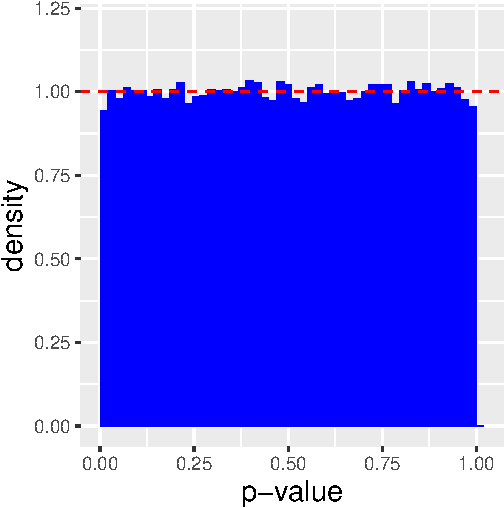
\includegraphics[keepaspectratio]{01-probability_files/figure-latex/fig-pval-1.pdf}}

}

\caption{\label{fig-pval}The empirical distribution of \(p\)-values
under the null hypothesis, for a lower-tail test with \(n = 20\),
\(\mu_o = 3\), and \(\sigma^2 = 1\). We can see that the \(p\)-values
are uniformly distributed between 0 and 1 (with some random variation
due to the fact that our simulation contains a finite sample of data).
When the null is true, the probability of sampling a \(p\)-value less
than \(\alpha\) is thus exactly \(\alpha\).}

\end{figure}%

\begin{quote}
Because we are performing a simulation, the number of observations
falling into each histogram bin is a random variable, and thus we
observe some amount of ``noise'' in Figure~\ref{fig-pval} (i.e., some
amount of variation around the dashed red line)\ldots but nevertheless
we can visually infer that the sampling distribution for \(p\) is
uniform (i.e., flat). (For completeness, the number of counts in each
bin are collectively sampled from a multinomial distribution, where the
probability of a count being recorded in any given bin being the
reciprocal of the number of bins. We introduce the multinomial
distribution in Section~\ref{sec-chap3multi}.)
\end{quote}

\begin{quote}
Now, what if the null hypothesis is not correct? What will happen to the
distribution of \(p\)-values? The answer depends on the circumstance: if
we are performing an lower-tail test (with \(E[Y]\) increasing with
\(\theta\)) and the true mean is \emph{larger} than the hypothesized
mean, then the \(p\)-values will skew towards 1: we are less likely to
reject the null when its value is closer to the tail of interest than
the true value is. If the true mean is smaller than the hypothesized
mean, the \(p\)-values will skew towards 0. See
Figure~\ref{fig-pvalskew} for a demonstration of the latter point.
\end{quote}

\begin{verbatim}
The proportion of p-values < 0.05 is  0.29707 
\end{verbatim}

\begin{figure}

\centering{

\pandocbounded{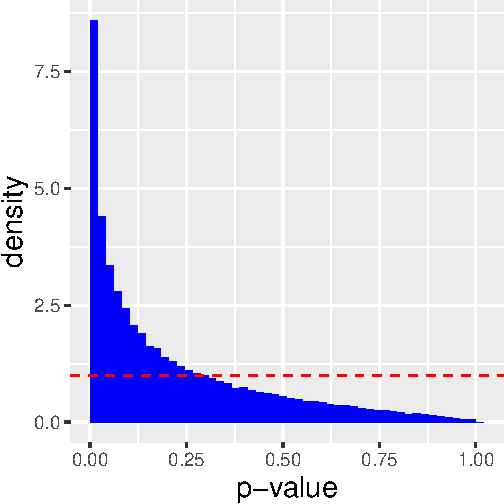
\includegraphics[keepaspectratio]{01-probability_files/figure-latex/fig-pvalskew-1.pdf}}

}

\caption{\label{fig-pvalskew}The empirical distribution of \(p\)-values
when the stated alternative hypothesis is consistent with the truth. We
can see that the \(p\)-values skew towards 0, meaning that when the
alternative hypothesis is true, the probability of sampling a
\(p\)-value less than \(\alpha\) can be \(\gg \alpha\).}

\end{figure}%

\begin{quote}
In Figure~\ref{fig-pvalskew}, 29.71\% of the counts are observed as
having value less than \(\alpha = 0.05\)\ldots so we are more likely to
reject the null. And as the true mean gets smaller and smaller than
\(\mu_o = 3\), the number of counts in the first bins will
increase\ldots meaning that null becomes more and more easily rejected.
This example foreshadows the concept of \emph{hypothesis test power},
which we introduce in Section~\ref{sec-chap2power}.
\end{quote}

\begin{quote}
We will make three important statements about \(p\)-values here, ones
that are good for all readers to remember.
\end{quote}

\begin{quote}
\begin{enumerate}
\def\labelenumi{\arabic{enumi}.}
\tightlist
\item
  \textbf{A p-value is not the probability that the null hypothesis is
  correct!} A hypothesis is \emph{not} a random variable, and there is
  thus no probability associated with it. A \(p\)-value is the
  probability of observing a more extreme hypothesis test statistic than
  what we actually observe, conditioned on the null hypothesis being
  correct.
\end{enumerate}
\end{quote}

\begin{quote}
\begin{enumerate}
\def\labelenumi{\arabic{enumi}.}
\setcounter{enumi}{1}
\tightlist
\item
  \textbf{We cannot select the Type I error rate \(\alpha\) after
  computing the p-value.} We specify the Type I error rate \(\alpha\)
  \emph{before} data are analyzed; specifying it afterwards opens up the
  analysis procedure to bias: ``my \(p\)-value is 0.09\ldots so I'll set
  \(\alpha = 0.1\) so that I can reject the null.''
\end{enumerate}
\end{quote}

\begin{quote}
\begin{enumerate}
\def\labelenumi{\arabic{enumi}.}
\setcounter{enumi}{2}
\tightlist
\item
  \textbf{We cannot perform multiple hypothesis tests without correcting
  our result.} Suppose that we perform 100 independent hypothesis tests,
  each with \(\alpha = 0.05\). Even if the null is true for every test,
  we will end up rejecting the null approximately five times. (Not
  necessarily exactly five times: the number of rejections we observe is
  a random variable with mean of five.) That we will reject an
  increasing number of null hypotheses with an increasing number of
  tests is inevitable: this is a feature of hypothesis testing, not a
  bug. When performing multiple tests, we need to apply a correction
  factor to each observed \(p\)-value, such as a Bonferroni correction
  (e.g., if \(m\) is the number of conducted tests, reset \(\alpha\) to
  \(\alpha/m\)) or the less conservative false-discovery rate (FDR)
  correction. Otherwise, we are engaging in \emph{p-hacking} and
  \emph{data dredging}. We discuss correction factors in more detail in
  Section~\ref{sec-chap7multiple}.
\end{enumerate}
\end{quote}

\subsubsection{Simulation: Estimating a
p-Value}\label{simulation-estimating-a-p-value}

\begin{quote}
In the second example above, we determine that if we sample a statistic
\(Y\) from the distribution \(f_Y(y) = \theta (1-y)^{\theta-1}\), with
\(y \in [0,1]\), and if \(\theta_o = 1\) and \(y_{\mathrm{obs}} = 0.9\),
then the \(p\)-value is 0.01. Here, we show how we can compute a
\(p\)-value via simulations.
\end{quote}

\begin{quote}
As a reminder, we have identified \(f_Y(y)\) as being part of the beta
family of distributions, which we officially introduce in
Section~\ref{sec-chap3beta}; thus we can utilize \texttt{rbeta()} like
we do in the last example above.
\end{quote}

\begin{Shaded}
\begin{Highlighting}[]
\FunctionTok{set.seed}\NormalTok{(}\DecValTok{101}\NormalTok{)}

\NormalTok{n        }\OtherTok{\textless{}{-}} \DecValTok{1}
\NormalTok{num.sim  }\OtherTok{\textless{}{-}} \DecValTok{10000}
\NormalTok{theta.o  }\OtherTok{\textless{}{-}} \DecValTok{2}
\NormalTok{y.obs    }\OtherTok{\textless{}{-}} \FloatTok{0.9}

\NormalTok{Y        }\OtherTok{\textless{}{-}} \FunctionTok{rbeta}\NormalTok{(n }\SpecialCharTok{*}\NormalTok{ num.sim, }\DecValTok{1}\NormalTok{, theta.o)}

\NormalTok{(p       }\OtherTok{\textless{}{-}} \FunctionTok{sum}\NormalTok{(Y }\SpecialCharTok{\textgreater{}=}\NormalTok{ y.obs) }\SpecialCharTok{/}\NormalTok{ num.sim)}
\end{Highlighting}
\end{Shaded}

\begin{verbatim}
[1] 0.0108
\end{verbatim}

\begin{quote}
Our estimated \(p\)-value is 0.0108: in 108 of the 10000 simulated
experiments, the observed statistic was equal to or greater than what we
observed in our one actual experiment. Because we do not perform an
infinite number of simulations, the estimated \(p\)-value is a random
variable, and we do not expect it to match the true value of 0.01
exactly. What we observe is very strong evidence that our simulated
\(p\)-value is both a precise and accurate estimate of the true value.
In Section~\ref{sec-chap3confidence}, we will learn how to turn this
evidence into something more firmly quantitative.
\end{quote}

\section{Exercises}\label{sec-chap1exercises}

\begin{enumerate}
\def\labelenumi{\arabic{enumi}.}
\item
  We are given that for the events \(A\) and \(B\),
  \(P(A \vert B) = P(B \vert A)\). We are also given that
  \(P(\bar{A} \cap \bar{B}) = 0.2\). Express \(P(A \cap B)\) as a
  function of \(P(A)\).
\item
  We are given that \(A \subset B\) and that \(P(A) > 0\) and
  \(0 < P(B) < 1\). Can the events \(A\) and \(B\) be independent
  events?
\item
  Re-express the conditional probability \(P(A \cap B \vert A \cup B)\)
  in terms of two unconditional probabilities that reference only the
  events \(\bar{A}\) and \(\bar{B}\).
\item
  We are given that \(P(B) = 1/2\), \(P(B \vert A) = 1/4\), and
  \(P(A \vert \bar{B}) = 1/3\). (a) What is \(P(A \cap B)\)? (b) What is
  \(P(B \vert \bar{A})\)?
\item
  Re-express the probability \(P(\bar{A} \vert \bar{B})\) as a function
  of \(A\) and \(B\) only.
\item
  We draw two balls from an urn containing two white and three black
  balls, without replacement. What is the probability that the second
  drawn ball is black?
\item
  A student answers a multiple-choice question with five possible
  answers. Assume the probability that the student knows the answer is
  0.6 (and thus that the probability that the student will guess is
  0.4). Also assume that the probability of getting the question right
  when guessing is 0.2. If the student gets the question right, what is
  the probability that he knew the answer?
\item
  A study of the residents of a region showed that 15 percent were
  smokers. The probability of death due to lung cancer, given that a
  person smoked, was ten times the probability of death due to lung
  cancer, given that the person did not smoke. If the probability of
  death due to lung cancer in the region is 0.01, what is the
  probability that a person was a smoker, given that he or she died of
  lung cancer?
\item
  We play a particular game in which we roll a \emph{fair} three-sided
  die. (Assume one exists!) We repeatedly roll the die until we fail to
  roll a 1. Our score is the total sum of all rolls, including the last
  roll. We win the game if our score is \emph{greater} than 3. What is
  the probability that we win a single instance of this game? (It may
  help to recall that if we have a sequence of events
  \{\(A,BA,BBA,...\)\}, with associated unchanging probabilities
  \(P(A)\) and \(P(B)\), then the sum of the event probabilities is
  \(P(A)/[1-P(B)]\).)
\item
  We are given a coin with a memory. Let \(H_i\) and \(T_i\) denote the
  events of observing heads and tails on the \(i^{\mathrm{th}}\) flip,
  respectively. Assume \(P(H_1) = P(T_1) = 0.5\), and that
  \(P(H_{i+1} \vert T_i) = 0.6\) and \(P(T_{i+1} \vert H_i) = 0.3\).
  Compute \(P(H_1 \cup T_2)\).
\item
  If a water specimen contains nitrates, a solution dropped into it will
  cause it to turn red 90 percent of the time. When used on water
  specimens without nitrates, the solution causes the water to turn red
  15 percent of the time. Nitrates exist in 20 percent of the specimens.
  (a) What is the probability that a randomly selected specimen will
  turn red when tested? (b) What is the probability that a randomly
  selected specimen contains nitrates, if it turns red when tested?
\item
  Of travelers arriving at a small airport, 60 percent fly on major
  airlines, 30 percent on private planes, and 10 percent on other
  aircraft. Of those on the major airlines, 50 percent travel for
  business, while 60 percent of the private plane takers are business
  travelers and 90 percent of those on other aircraft are business
  travelers. We select a traveler at random. (a) What is the probability
  that he or she is a business traveler? (b) What is the probability
  that he or she arrived on a private plane, given that he or she is a
  business traveler?
\item
  We have an urn with four balls, two of which are red and two of which
  are black, and we sample without replacement from the urn. Let \(X\)
  be the number of draws that we make until the first red ball is drawn.
  (a) What is the expected value of \(X\)? (b) What is the variance of
  \(X\)?
\item
  We possess three bowls that are labeled 1, 2, and 3. Bowl 1 contains
  one white and two black balls. Bowl 2 contains two white and one black
  balls. Bowl 3 contains three white balls. We select a bowl at random,
  and then sample two balls from that bowl, without replacement. (a)
  What is the probability of observing two white balls? (b) Given that
  we observe two white balls, what is the probability that they were
  sampled from bowl number 3?
\item
  Two methods are available for learning a certain skill, method \(A\)
  and method \(\bar{A}\). Method \(A\) is less expensive, and thus it is
  used 80 percent of the time (with method \(\bar{A}\) being used the
  rest of the time). Let \(F\) be the event of failing to learn the
  skill: if method \(A\) is used, the failure rate is 20 percent, while
  for \(\bar{A}\) the rate is 10 percent. (a) What is the probability of
  failure, \(P(F)\)? (b) What is the probability that a person who
  failed was taught using method \(A\)?
\item
  Below we display a (partially known) probability mass function. We
  know that \(E[X] = 1.6\). What is
  \(P(\mu - \sigma \leq X \leq \mu + \sigma)\)?
\end{enumerate}

{\def\LTcaptype{none} % do not increment counter
\begin{longtable}[]{@{}cc@{}}
\toprule\noalign{}
\(x\) & \(p_X(x)\) \\
\midrule\noalign{}
\endhead
\bottomrule\noalign{}
\endlastfoot
0 & ? \\
1 & 0.5 \\
2 & ? \\
3 & 0.3 \\
\end{longtable}
}

\begin{enumerate}
\def\labelenumi{\arabic{enumi}.}
\setcounter{enumi}{16}
\item
  We are given the following pdf: \begin{align*}
  f_X(x) = \left\{ \begin{array}{cc} c/x^2 & 1 \leq x \leq 2 \\ 0 & \mbox{otherwise} \end{array} \right. \,.
  \end{align*} What is \(P(X > 1.25 \vert X < 1.5)\)?
\item
  We are given the following pdf: \begin{align*}
  f_X(x) = \left\{ \begin{array}{cc} c x^2 (1-x) & 0 \leq x \leq 1 \\ 0 & \mbox{otherwise} \end{array} \right. \,.
  \end{align*}
\end{enumerate}

\begin{enumerate}
\def\labelenumi{(\alph{enumi})}
\tightlist
\item
  What is \(c\)? (b) What is \(P(X > 1/2)\)? (c) What is \(E[X]\)?
\end{enumerate}

\begin{enumerate}
\def\labelenumi{\arabic{enumi}.}
\setcounter{enumi}{18}
\item
  We flip a fair coin two times. Let \(X_i\) denote the result of flip
  \(i\): \(X_i = 1\) for heads, and \(X_i = 0\) for tails. Now, let
  \(Y = \vert X_2 - X_1 \vert\). (a) What is the standard deviation of
  \(Y\)? (b) What is \(P(\mu - \sigma < Y < \mu + \sigma)\)?
\item
  We independently sample two data, \(X_1\) and \(X_2\), from the
  distribution \begin{align*}
  f_X(x) = 3x^2 ~~~ x \in [0,1] \,.
  \end{align*} (a) What is the mean of this distribution? (b) What is
  the variance of this distribution? (c) What is the mean of
  \(2X_1-2X_2\)? (d) What is the variance of \(2X_1-2X_2\)?
\item
  Let the cumulative distribution function \(F_X(x)\) be given by
  \begin{align*}
  F_X(x) = \left\{ \begin{array}{cc} 0 & x < 0 \\ x^3 & 0 \leq x \leq 1 \\ 1 & x > 1 \end{array} \right. \,.
  \end{align*} (a) Write down the probability density function. (b)
  Compute \(V[X]\). (c) What is the probability that an observed random
  variable \(X\) takes on a value less than 1/2, given that it is
  greater than 1/4?
\item
  Below we display a cumulative density function for a discrete random
  variable. What is \(V[X]\)?
\end{enumerate}

{\def\LTcaptype{none} % do not increment counter
\begin{longtable}[]{@{}ccccc@{}}
\toprule\noalign{}
\endhead
\bottomrule\noalign{}
\endlastfoot
& \(x <\) 0 & \(0 \leq x < 1\) & \(1 \leq x < 3\) & \(x \geq 3\) \\
\(F_X(x)\) & 0 & 0.5 & 0.75 & 1 \\
\end{longtable}
}

\begin{enumerate}
\def\labelenumi{\arabic{enumi}.}
\setcounter{enumi}{22}
\item
  We are given the following cumulative density function: \begin{align*}
  F_X(x) = \left\{ \begin{array}{cc} cx^2 & 0 \leq x \leq 1 \\ 0 & \mbox{otherwise} \end{array} \right. \,.
  \end{align*} (a) What is the value of \(c\)? (b) What is \(E[X]\)? (c)
  What is \(\sigma\)?
\item
  We are given the following probability density function:
  \begin{align*}
  f_X(x) = \left\{ \begin{array}{cc} a & 0 \leq x < 1 \\ bx & 1 \leq x < 2 \\ 0 & \mbox{otherwise} \end{array} \right. \,,
  \end{align*} where \(a\) and \(b\) are constants. (a) What is the
  largest value that \(b\) can have such that \(f_X(x)\) is a valid pdf?
  (b) Let \(a\) = 1/2 and \(b\) = 1/3. What is \(F_X(x)\)?
\item
  See the probability mass function table below. (a) If \(E[X] = 2\),
  what is the value of \(y\)? (b) If \(y = 3\), what is \(\sigma\) for
  this distribution? (c) Assume \(y = 3\). What is
  \(P(\mu-\sigma \leq X \leq \mu+\sigma)\)?
\end{enumerate}

{\def\LTcaptype{none} % do not increment counter
\begin{longtable}[]{@{}cccc@{}}
\toprule\noalign{}
\endhead
\bottomrule\noalign{}
\endlastfoot
\(x\) & 0 & 1 & \(y\) \\
\(p_X(x)\) & 0.4 & 0.4 & 0.2 \\
\end{longtable}
}

\begin{enumerate}
\def\labelenumi{\arabic{enumi}.}
\setcounter{enumi}{25}
\item
  We are given the following hybrid probability density/mass function:
  \begin{align*}
  g_X(x) = \left\{ \begin{array}{ll} 0.2 & x = -1 \\ c & x \in [0,1] \\ 0.2 & x = 2 \\ 0 & \mbox{otherwise} \end{array} \right. \,.
  \end{align*} (a) What is the value for \(c\)? (b) What is \(E[X]\)?
  (c) What is the cumulative distribution function \(F_X(x)\)?
\item
  We are given the probability density function \begin{align*}
  f_X(x) = \left\{ \begin{array}{ll} e^{-x} & x \in [0,\infty) \\ 0 & \mbox{otherwise} \end{array} \right. \,.
  \end{align*} (a) What is the cdf for \(x \geq 0\)? (b) What is
  \(P(X > 1)\)? (c) What is \(P(X < 1/2 \cup X > 2)\)? (d) What is the
  probability that \(X < 2\), given that \(X > 1\)?
\item
  We are given the probability density function \begin{align*}
  f_X(x) = \left\{ \begin{array}{ll} -x & x \in [-1,0) \\ x & x \in [0,1] \\ 0 & \mbox{otherwise} \end{array} \right. \,.
  \end{align*} (a) What is \(E[X]\)? (b) What is \(V[X]\)? (c) What is
  an expression for \(F_X(x)\) that is valid over the range
  \(x \in [0,1]\)?
\item
  We are given the following cumulative distribution function:
  \begin{align*}
  F_X(x) = \left\{ \begin{array}{ll} 0 & x \leq 0 \\ cx^2 & x \in (0,1] \\ 1 & x > 1 \end{array} \right. \,.
  \end{align*} (a) What is the value of \(c\) that makes \(f_X(x)\) a
  valid pdf? (b) What is \(E[X]\)?
\item
  We are given the following probability density function:
  \begin{align*}
  f_X(x) = \left\{ \begin{array}{cc} c & 0 \leq x < 1 \\ e^{-x} & 1 \leq x < \infty \\ 0 & \mbox{otherwise} \end{array} \right. \,,
  \end{align*} where \(c\) is a constant. (a) What is the value of \(c\)
  that makes \(f_X(x)\) a valid pdf? (b) What is the cumulative
  distribution function?
\item
  Below we display a probability mass function. (a) What is \(c\)? (b)
  What is the value of the cumulative distribution function at
  \(x=0.5\)? (c) What is the inverse cdf for \(q = 0.9\)? (d) What is
  the variance \(V[X]\)?
\end{enumerate}

{\def\LTcaptype{none} % do not increment counter
\begin{longtable}[]{@{}cccc@{}}
\toprule\noalign{}
\endhead
\bottomrule\noalign{}
\endlastfoot
\(x\) & -1 & 0 & 1 \\
\(p_X(x)\) & 1/6 & \(c\) & 1/6 \\
\end{longtable}
}

\begin{enumerate}
\def\labelenumi{\arabic{enumi}.}
\setcounter{enumi}{31}
\item
  We are given the following cumulative density function: \begin{align*}
  F_X(x) = x^3 \,,
  \end{align*} for \(x \in [0,1]\). (a) What is the probability density
  function, \(f_X(x)\), for \(x \in [0,1]\)? (b) What is
  \(P(1/4 \leq X \leq 3/4)\)? (c) What is
  \(P(X \leq 1/4 \vert X \leq 1/2)\)? (d) If \(q = F_X(x)\), what is the
  inverse cdf, i.e., what is \(F_X^{-1}(q)\)?
\item
  We draw three iid data \(\{X_1,X_2,X_3\}\) according to a probability
  distribution that has expected value \(\mu = 1\) and variance
  \(\sigma^2 = 1\). Let \(Y = X_1 + 2X_2 - 3X_3 - 4\). (a) What is
  \(E[Y]\)? (b) What is the variance of \(Y\)? (c) What is \(E[Y^2]\)?
\item
  We are working with a probability density whose domain is
  \(x \in [0,2]\), and we are given that \begin{align*}
  F_X(x) = cx^3
  \end{align*} within that domain. (a) What is the value of \(c\)? (b)
  What is \(f_X(x)\)? (c) What is \(P(X < 1/2 | X < 1)\)?
\item
  We sample a single datum \(X\) according to the probability density
  function \(\theta x^{\theta-1}\), with \(x \in [0,1]\). Let \(\theta\)
  itself be a random variable sampled according to a probability mass
  function with values 1/2 for \(\theta = 1\) and 1/2 for
  \(\theta = 2\). What is \(p_X(x)\) or \(f_X(x)\)? (Whichever is
  appropriate.)
\item
  We are given the following probability density function:
  \begin{align*}
  f_X(x) = 6 x (1-x) \,,
  \end{align*} for \(x \in [0,1]\). (a) What is \(E[X]\)? (b) Now assume
  that we have drawn \(n\) iid data according to this distribution and
  that we compute the sample mean \(\bar{X} = (1/n)\sum_{i=1}^n X_i\).
  What is \(E[\bar{X}]\)?
\item
  We are given the following probability density function:
  \begin{align*}
  f_X(x) = \frac{1}{2} ~~~ x \in [-1,1] \,,
  \end{align*} for which \(E[X] = \mu = 0\) and
  \(V[X] = \sigma^2 = 1/3\). We draw two iid data from this
  distribution, and we propose two estimators for \(\mu\):
  \(\hat{\mu}_1 = X_1-X_2\), and \((X_1+X_2)/2\). (a) What is the bias
  for each estimator? (b) What is the variance for each estimator? (c)
  What is the mean-squared error for each estimator. (d) Which estimator
  is better?
\item
  In an experiment, we sample \(n\) iid data that we assume were drawn
  according to the following probability density function:
  \begin{align*}
  f_X(x) = a (1+x)^{-(a+1)} \,,
  \end{align*} for \(x \geq 0\) and \(a > 0\). (a) What is the
  log-likelihood function \(\ell(a \vert \mathbf{x})\)? (b) What is the
  maximum likelihood estimate \(\hat{a}_{MLE}\)? (c) The mean of the
  distribution is \(\mu = 1/(a-1)\). What is \(\hat{\mu}_{MLE}\)?
\item
  We are given the following probability density function:
  \begin{align*}
  f_X(x) = \theta (1-x)^{\theta - 1} \,,
  \end{align*} where \(x \in [0,1]\) and \(\theta > 0\). Assume that we
  have sampled \(n\) iid data according to this pdf. (a) What is the
  log-likelihood \(\ell(\theta \vert \mathbf{x})\)? (b) What is the
  maximum-likelihood estimate for \(\theta\)? (c) For the distribution
  above, the population mean is \(\mu = E[X] = 1/(1+\theta)\). What is
  the MLE for \(\mu\)?
\item
  We are given \(n\) iid data that were sampled according to the
  following probability density function: \begin{align*}
  f_X(x) = \alpha x^{\alpha-1} \,,
  \end{align*} with \(\alpha > 0\) and \(0 \leq x \leq 1\). What is the
  maximum likelihood estimator for \(\alpha\)?
\item
  We are given \(n\) iid data that are sampled according to the
  following probability mass function: \begin{align*}
  p_X(x) = (1-p)^{x-1}p \,,
  \end{align*} with \(0 < p < 1\) and \(x = \{1,2,3,\ldots\}\). For this
  distribution, \(E[X] = 1/p\) and \(V[X] = (1-p)/p^2\). (a) What is the
  maximum likelihood estimator for \(1/p\)? (b) Write down
  \(V[\widehat{1/p}_{MLE}]\), i.e., the variance of the MLE for \(1/p\).
\item
  We sample \(n\) iid data according to the following probability
  density function: \begin{align*} 
  f_X(x) = 1 ~~~ x \in \left[ \theta - \frac12 , \theta + \frac12 \right]
  \end{align*} For this distribution, \(E[X] = \theta\) and
  \(V[X] = \theta^2/12\). A friend, who didn't really think things
  through, suggested \(\hat{\theta} = (X_1 - X_2)/2\) as an estimator
  for \(\theta\). It is up to us to characterize this estimator. (a)
  What is the bias of \(\hat{\theta}\)? (b) What is the variance of
  \(\hat{\theta}\)? (c) What is the mean-squared error for
  \(\hat{\theta}\)? (d) One of us suggests changing the minus sign in
  the estimator to a plus sign: that at least makes the estimator
  unbiased. What is the mean-squared error for this new estimator?
\item
  We sample \(n\) iid data according to an exponential distribution:
  \begin{align*}
  f_X(x) = \frac{1}{\theta} e^{-x/\theta} \,,
  \end{align*} where \(x \geq 0\) and \(\theta > 0\). For this
  distribution, \(E[X] = \theta\) and \(V[X] = \theta^2\). We propose
  the estimator \(\hat{\theta} = X_1 - X_2/n\). (a) What is the bias for
  this estimator? (b) What is the variance for this estimator?
\item
  We are given a sample of \(n\) iid data drawn according to the
  probability density function \begin{align*}
  f_X(x) = c e^{-\theta x} \theta^{x-1} \,,
  \end{align*} where \(\theta \in [0,1]\), \(c > 0\), and \(x\) is a
  positive integer. (a) What is the log-likelihood function? (b) What is
  the maximum likelihood estimate for \(\theta\)? (c) The mean of this
  distribution is \(\mu = 1/(1-\theta)\). What is the MLE for \(\mu\)?
\item
  We sample a single datum \(X = x_{\mathrm{obs}}\) according to the
  following probability density function: \begin{align*}
  f_X(x) = a(1+x)^{-a-1} \,,
  \end{align*} where \(x \geq 0\) and where we will assume \(a > 1\).
  Let the statistic \(Y = X\); the expected value for \(Y\) is
  \(E[Y] = 1/(a-1)\). (a) What is \(F_Y(y)\)? (b) Given
  \(\alpha = 0.05\), derive a lower bound on the parameter \(a\).
\item
  A logistic distribution with scale parameter 1 has the probability
  density function \begin{align*}
  f_X(x) = \frac{\exp[-(x-\mu)]}{(1+\exp[-(x-\mu)])^2} \,,
  \end{align*} for \(x\) and \(\mu\) both \(\in (-\infty,\infty)\). The
  cumulative distribution function is \begin{align*}
  F_X(x) = \frac{1}{1+\exp[-(x-\mu)]} \,,
  \end{align*} and the expected value of \(X\) is \(E[X] = \mu\). We
  draw a single datum \(X\) from this distribution. Let the statistic
  \(Y = X\). (a) What is the rejection region boundary for a lower-tail
  test given the null hypothesis \(H_o : \mu = \mu_o = 0\)? Assume
  \(\alpha\) = 0.05. (b) For the test in (a), if
  \(y_{\mathrm{obs}} > y_{\mathrm{RR}}\), do we reject the null
  hypothesis, or fail to reject the null hypothesis? (c) If instead we
  were to perform a two-tail test given the same value of \(\alpha\),
  would the new lower rejection region boundary be further from
  \(\mu_o\) than the boundary you found in part (a), or closer to
  \(\mu_o\)?
\item
  In an experiment, you sample a single datum \(X\) from a distribution
  whose cumulative distribution function is \begin{align*}
  F_X(x) = e^{-e^{-(x-\theta)}} \,,
  \end{align*} where \(x \in (-\infty,\infty)\) and
  \(\theta \in (-\infty,\infty)\). The statistic is \(Y = X\); its
  observed value is \(y_{\mathrm{obs}} = x_{\mathrm{obs}}\). The
  expected value of the \(Y\) is \(E[Y] = \theta + \gamma\), where
  \(\gamma\) is a constant. (a) Write down a one-sided
  \(100(1-\alpha)\)-percent upper bound for \(\theta\). (b) Write down
  the \emph{lower} bound for a two-sided \(100(1-\alpha)\)-percent
  confidence interval for \(\theta\). No explicit work need be shown for
  part (b), where it is possible to reason out the answer without math.
\item
  In an experiment, you sample a single datum \(X\) from a distribution
  whose cumulative distribution function is \begin{align*}
  F_X(x) = 1 - e^{-(x-2)/\theta} \,,
  \end{align*} for \(x \geq 2\) and \(\theta > 0\). The statistic is
  \(Y = X\); its observed value is
  \(y_{\mathrm{obs}} = x_{\mathrm{obs}}\). The expected value of \(X\)
  is \(E[X] = \theta + 2\). (a) Write down the rejection-region boundary
  for the upper-tail test \(H_o : \theta = \theta_o = 1\) versus
  \(H_a : \theta > \theta_o\). Assume the Type I error is \(\alpha\).
  (b) If \(y_{\mathrm{obs}} < y_{\mathrm{RR}}\), what conclusion do you
  reach: ``reject'' (the null) or ``fail to reject''? (c) Write down the
  \emph{lower} rejection-region boundary for the two-tail test
  \(H_o : \theta = \theta_o = 1\) versus \(H_a : \theta \neq \theta_o\).
  No explicit work need be shown for part (c), where it is possible to
  reason out the answer without math.
\end{enumerate}

\bookmarksetup{startatroot}

\chapter{The Normal (and Related) Distributions}\label{sec-chap2}

In this chapter, we illustrate probability and statistical inference
concepts utilizing the \emph{normal distribution}. The normal, also
known in the physical sciences as the Gaussian distribution and,
colloquially, the ``bell curve,'' is the most utilized probability
distribution in all of data analysis.

Why are we choosing to focus on the normal distribution now, in this
chapter?

\begin{enumerate}
\def\labelenumi{\arabic{enumi}.}
\tightlist
\item
  We often observe that the data that we generate in experiments are at
  least approximately normally distributed. And while other, more
  general families of distributions (such as the gamma distribution)
  might explain the data-generating process as well as the normal
  distribution does, it has the advantage of having intuitively
  easy-to-understand parameters: \(\mu\) for the mean, and \(\sigma^2\)
  for the variance (meaning that \(\sigma\) directly indicates the
  ``width'' of the region on the real-number line over which \(f_X(x)\)
  is effectively non-zero).
\item
  The normal distribution is the limiting distibution for many other
  distributions (i.e., there are many families of distributions that,
  with the right choice(s) for parameter value(s), can mimic the shape
  of the normal).
\item
  The normal distribution figures prominently in the Central Limit
  Theorem, which states that if we sample a sufficiently large number of
  data according to any distribution with finite variance, we can assume
  the sample mean to be approximately normally distributed.
\end{enumerate}

\section{Normal Distribution: Probability Density
Function}\label{sec-chap2pdf}

What to take away from this section:

\begin{itemize}
\item
  The normal distribution is a continuous, symmetric distribution with a
  probability density function whose shape and location along the
  real-number line is governed by two parameters: \(\mu\), the
  population mean, and \(\sigma^2\), the population variance.
\item
  The \emph{empirical rule}: (very nearly) all data sampled according to
  a normal distribution lie in the range
  \([\mu - 3\sigma,\mu + 3\sigma]\), even though the domain of the
  distribution is \((-\infty,\infty)\).
\end{itemize}

\smallskip\hrule

\begin{quote}
\textbf{Recall}: \emph{a probability density function is one way to
represent a continuous probablity distribution, and it has the
properties (a) \(f_X(x) \geq 0\) and (b) \(\int_x f_X(x) dx = 1\), where
the integral is over all values of \(x\) in the distribution's domain.}
\end{quote}

\smallskip\hrule

Let \(X\) be a continuous random variable sampled according to a normal
distribution with mean \(\mu\) and variance \(\sigma^2\), i.e., let
\(X \sim \mathcal{N}(\mu,\sigma^2)\). The pdf for \(X\) is \[
f_X(x) = \frac{1}{\sqrt{2\pi\sigma^2}} \exp\left(-\frac{(x-\mu)^2}{2\sigma^2}\right) ~~~~~~ x \in (-\infty,\infty) \,.
\] This pdf is symmetric around \(\mu\) (see Figure~\ref{fig-normpdf}),
with the area under the curve approaching 1 over the range
\(\mu - 3\sigma \leq x \leq \mu + 3\sigma\). (The value of the integral
of \(f_X(x)\) over this range is 0.9973. This gives rise to one aspect
of the so-called \emph{empirical rule}: if data are sampled according to
a normal or normal-like distribution, we expect (nearly) all of the data
to lie with three standard deviations of the population mean.)

\begin{figure}

\centering{

\pandocbounded{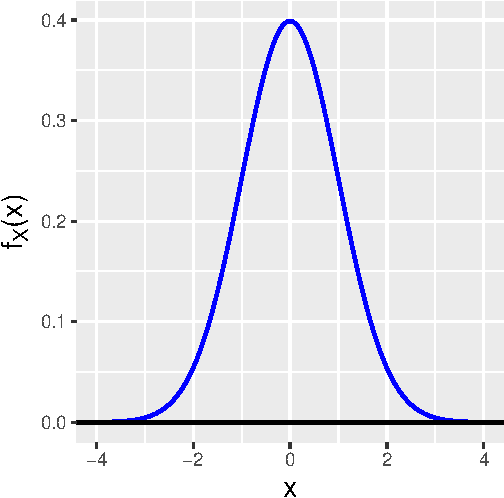
\includegraphics[keepaspectratio]{02-normal_files/figure-latex/fig-normpdf-1.pdf}}

}

\caption{\label{fig-normpdf}A normal probability density function with
mean 0 and standard deviation 1.}

\end{figure}%

\subsection{Examples}\label{examples-13}

\subsubsection{Expected Value and
Variance}\label{expected-value-and-variance}

\smallskip\hrule

\begin{quote}
\textbf{Recall:} \emph{the expected value of a continuously distributed
random variable is} \[
E[X] = \int_x x f_X(x) dx\,,
\] \emph{where the integral is over all values of \(x\) within the
domain of the pdf \(f_X(x)\). The expected value is equivalent to a
weighted average, with the weight for each possible value of \(x\) given
by \(f_X(x)\).}
\end{quote}

\smallskip\hrule

\begin{quote}
The expected value of a normal random variable \(X\) is \[
E[X] = \int_{-\infty}^\infty x \frac{1}{\sqrt{2\pi\sigma^2}} \exp\left(-\frac{(x-\mu)^2}{2\sigma^2}\right) dx
\] To evaluate this integral, we implement variable substitution. Recall
that the three steps of variable substitution are\ldots{}
\end{quote}

\begin{enumerate}
\def\labelenumi{\arabic{enumi}.}
\tightlist
\item
  to write down a viable substitution \(u = g(x)\);
\item
  to then derive \(du = h(u,x) dx\); and finally
\item
  to use \(u = g(x)\) to transform the bounds of the integral.
\end{enumerate}

\begin{quote}
Because the integral bounds here are \(-\infty\) and \(\infty\), we
choose \(u = g(x)\) such that we rewrite \((x-\mu)^2/\sigma^2\) as
\(u^2\), so that eventually, as we will see, what remains in the
integrand is a normal pdf for \(\mu = 0\) and \(\sigma^2 = 1\): \[
(1) ~~ u = \frac{x-\mu}{\sigma} ~~ \implies ~~ (2) ~~ du = \frac{1}{\sigma}dx
\] and \[
(3) ~~ x = -\infty ~\implies~ u = -\infty ~~~ \mbox{and} ~~~ x = \infty ~\implies~ u = \infty \,,
\] Thus \begin{align*}
E[X] &= \int_{-\infty}^\infty (\sigma u + \mu) \frac{1}{\sqrt{2\pi\sigma^2}} \exp\left(-\frac{u^2}{2}\right) \sigma du \\
&= \int_{-\infty}^\infty \frac{\sigma u}{\sqrt{2 \pi}} \exp\left(-\frac{u^2}{2}\right) du + \int_{-\infty}^\infty \frac{\mu}{\sqrt{2 \pi}} \exp\left(-\frac{u^2}{2}\right) du
\end{align*} The first integrand is the product of an odd function
(\(u\)) and an even function (\(\exp(-u^2/2)\)), and thus the first
integral evaluates to zero. As for the second integral: \[
E[X] = \int_{-\infty}^\infty \frac{\mu}{\sqrt{2 \pi}} \exp\left(-\frac{u^2}{2}\right) du = \mu \int_{-\infty}^\infty \frac{1}{\sqrt{2 \pi}} \exp\left(-\frac{u^2}{2}\right) du = \mu \,.
\] As stated above, the integrand is a normal pdf with parameters
\(\mu = 0\) and \(\sigma^2\) = 1, and since the bounds of the integral
match that of the domain of the normal pdf, the value of the integral is
1.
\end{quote}

\smallskip\hrule

\begin{quote}
\textbf{Recall:} \emph{the variance of a continuously distributed random
variable is} \[
V[X] = \int_x (x-\mu)^2 f_X(x) dx = E[X^2] - (E[X])^2\,,
\] \emph{where the integral is over all values of \(x\) within the
domain of the pdf \(f_X(x)\). The variance represents the square of the
``width'' of a probability density function, where by ``width'' we mean
the range of values of \(x\) for which \(f_X(x)\) is effectively
non-zero.}
\end{quote}

\smallskip\hrule

\begin{quote}
Here, \(V[X] = E[X^2] - (E[X])^2 = E[X^2] - \mu^2\). To determine
\(E[X^2]\), we implement a similar variable substitution to the one
above, except that now \begin{align*}
E[X^2] &= \int_{-\infty}^\infty (\sigma t + \mu)^2 \frac{1}{\sqrt{2\pi\sigma^2}} \exp\left(-\frac{t^2}{2}\right) \sigma dt \\
&= \int_{-\infty}^\infty \frac{\sigma^2 t^2}{\sqrt{2 \pi}} \exp\left(-\frac{t^2}{2}\right) dt + \int_{-\infty}^\infty \frac{2 \mu \sigma t}{\sqrt{2 \pi}} \exp\left(-\frac{t^2}{2}\right) dt\\
&~~~~ + \int_{-\infty}^\infty \frac{\mu^2}{\sqrt{2 \pi}} \exp\left(-\frac{t^2}{2}\right) dt \,.
\end{align*} The second integral is that of an odd function and thus
evaluates to zero, and the third integral is, given results above,
\(\mu^2\). This leaves \[
E[X^2] = \int_{-\infty}^\infty \frac{\sigma^2 t^2}{\sqrt{2 \pi}} \exp\left(-\frac{t^2}{2}\right) dt + \mu^2 \,.
\] or \[
V[X] = \frac{\sigma^2}{\sqrt{2 \pi}} \int_{-\infty}^\infty t^2 \exp\left(-\frac{t^2}{2}\right) dt \,.
\] As the integrand is \emph{not} a normal pdf, we need to pursue
integration by parts. Setting aside the constants outside the integral,
we have that \[
\begin{array}{ll} u = -t & dv = -t \exp(-t^2/2) dt \\ du = -dt & v = \exp(-t^2/2) \end{array} \,,
\] and so \begin{align*}
\int_{-\infty}^\infty t^2 \exp\left(-\frac{t^2}{2}\right) dt &= \left. uv \right|_{-\infty}^{\infty} - \int_{-\infty}^\infty v du \\
&= - \left. t \exp(-t^2/2) \right|_{-\infty}^{\infty} + \int_{-\infty}^\infty \exp(-t^2/2) dt \\
&= 0 + \sqrt{2\pi} \int_{-\infty}^\infty \frac{1}{\sqrt{2\pi}} \exp(-t^2/2) dt \\
&= \sqrt{2\pi} \,.
\end{align*} The first term evaluates to zero between for each bound, as
\(e^{-t^2/2}\) goes to zero much faster than \(\vert t \vert\) goes to
infinity. As for the second term: we recognize that the integrand is a
normal pdf with mean zero and variance one\ldots so the integral by
definition evaluates to 1. In the end, after restoring the constants we
set aside above, we have that \[
V[X] = \frac{\sigma^2}{\sqrt{2 \pi}} \sqrt{2\pi} = \sigma^2 \,.
\]
\end{quote}

\subsubsection{Skewness}\label{skewness}

\begin{quote}
The \emph{skewness} of a pmf or pdf is a metric that indicates its level
of asymmetry. Fisher's moment coefficient of skewness is \[
E\left[\left(\frac{X-\mu}{\sigma}\right)^3\right] \,.
\] which, expanded out, becomes \[
\frac{E[X^3] - 3 \mu \sigma^2 - \mu^3}{\sigma^3} \,.
\] What is the skewness of the normal distribution? At first, this
appears to require a long and involved series of integrations so as to
solve \(E[X^3]\). But let's try to be more clever.
\end{quote}

\begin{quote}
We know, from above, that the quantity \((\sigma t + \mu)^3\) will
appear in the integral for \(E[X^3]\). Let's expand this out: \[
\sigma^3 t^3 + 3 \sigma^2 \mu t^2 + 3 \sigma \mu^2 t + \mu^3 \,.
\] Each of these terms will appear separately in integrals of
\(\exp(-t^2/2)/\sqrt{2\pi}\) over the domain \(-\infty\) to \(\infty\).
From above, what do we already know? First, we know that if \(t\) is
raised to an odd power, the integral will be zero. This eliminates
\(\sigma^3 t^3\) and \(3 \sigma \mu^2 t\). Second, we know that for the
\(t^0\) term, the result will be \(\mu^3\), and we know that for the
\(t^2\) term, the result will be \(3 \sigma^2 \mu\). Thus \[
E[X^3] = 3\sigma^2\mu + \mu^3
\] and the skewness is \[
\frac{3 \mu \sigma^2 + \mu^3 - 3 \mu \sigma^2 - \mu^3}{\sigma^3} = 0 \,.
\] The skewness is zero, meaning that a normal pdf is symmetric around
its mean \(\mu\).
\end{quote}

\subsubsection{Computing Probabilities}\label{computing-probabilities}

\begin{quote}
Before diving into this example, we will be clear that this is
\emph{not} the optimal way to compute probabilities associated with
normal random variables, as we should utilize \texttt{R}'s
\texttt{pnorm()} function, as shown in the next section. However,
showing how to utilize \texttt{integrate()} is useful review. (We also
show how to pass distribution parameters to \texttt{integrate()}, which
we did not do in Section~\ref{sec-chap1working}.)
\end{quote}

\begin{quote}
\begin{enumerate}
\def\labelenumi{\arabic{enumi}.}
\tightlist
\item
  If \(X \sim \mathcal{N}(10,4)\), what is \(P(8 \leq X \leq 13.5)\)?
\end{enumerate}
\end{quote}

\begin{quote}
To find this probability, we integrate over the normal pdf with mean
\(\mu = 10\) and variance \(\sigma^2 = 4\). Visually, we are determining
the area of the red-shaded region in Figure~\ref{fig-pdfint}.
\end{quote}

\begin{figure}

\centering{

\pandocbounded{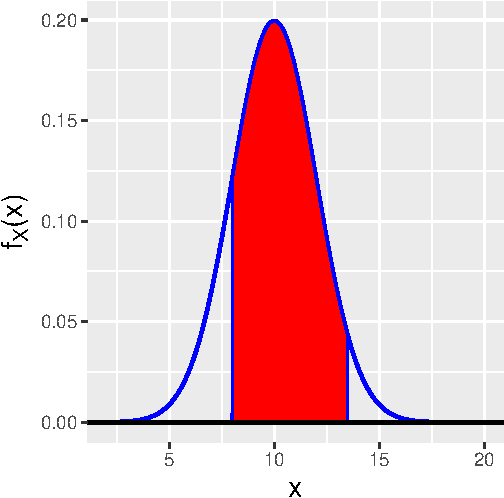
\includegraphics[keepaspectratio]{02-normal_files/figure-latex/fig-pdfint-1.pdf}}

}

\caption{\label{fig-pdfint}The probability \(P(8 \leq X \leq 13.5)\) is
the area of the red-shaded region, i.e., the integral of the normal
probability density function from 8 to 13.5, assuming \(\mu = 10\) and
\(\sigma^2 = 4\).}

\end{figure}%

\begin{Shaded}
\begin{Highlighting}[]
\NormalTok{integrand }\OtherTok{\textless{}{-}} \ControlFlowTok{function}\NormalTok{(x,mu,sigma2) \{}
  \FunctionTok{return}\NormalTok{(}\FunctionTok{exp}\NormalTok{(}\SpecialCharTok{{-}}\NormalTok{(x}\SpecialCharTok{{-}}\NormalTok{mu)}\SpecialCharTok{\^{}}\DecValTok{2}\SpecialCharTok{/}\DecValTok{2}\SpecialCharTok{/}\NormalTok{sigma2)}\SpecialCharTok{/}\FunctionTok{sqrt}\NormalTok{(}\DecValTok{2}\SpecialCharTok{*}\NormalTok{pi}\SpecialCharTok{*}\NormalTok{sigma2))}
\NormalTok{\}}
\FunctionTok{integrate}\NormalTok{(integrand,}\DecValTok{8}\NormalTok{,}\FloatTok{13.5}\NormalTok{,}\AttributeTok{mu=}\DecValTok{10}\NormalTok{,}\AttributeTok{sigma2=}\DecValTok{4}\NormalTok{)}\SpecialCharTok{$}\NormalTok{value}
\end{Highlighting}
\end{Shaded}

\begin{verbatim}
[1] 0.8012856
\end{verbatim}

\begin{quote}
The result is 0.801. Note how the \texttt{integrand()} function requires
extra information above and beyond the value of \texttt{x}. This
information is passed in using the extra arguments \texttt{mu} and
\texttt{sigma2}, the values of which are set in the call to
\texttt{integrate()}.
\end{quote}

\begin{quote}
\begin{enumerate}
\def\labelenumi{\arabic{enumi}.}
\setcounter{enumi}{1}
\tightlist
\item
  If \(X \sim \mathcal{N}(13,5)\), what is
  \(P(8 \leq X \leq 13.5 \vert X < 14)\)?
\end{enumerate}
\end{quote}

\begin{quote}
Recall that
\(P(a \leq X \leq b \vert X \leq c) = P(a \leq X \leq b)/P(X \leq c)\),
assuming that \(a < b < c\). So this probability is, visually, the ratio
of the area of the brown-shaded region in Figure~\ref{fig-pdfcond} to
the area of the red-shaded region underlying it. We can reuse the
\texttt{integrand()} function from above, calling it twice:
\end{quote}

\begin{Shaded}
\begin{Highlighting}[]
\FunctionTok{integrate}\NormalTok{(integrand,}\DecValTok{8}\NormalTok{,}\FloatTok{13.5}\NormalTok{,}\AttributeTok{mu=}\DecValTok{13}\NormalTok{,}\AttributeTok{sigma2=}\DecValTok{5}\NormalTok{)}\SpecialCharTok{$}\NormalTok{value }\SpecialCharTok{/} 
  \FunctionTok{integrate}\NormalTok{(integrand,}\SpecialCharTok{{-}}\ConstantTok{Inf}\NormalTok{,}\DecValTok{14}\NormalTok{,}\AttributeTok{mu=}\DecValTok{13}\NormalTok{,}\AttributeTok{sigma2=}\DecValTok{5}\NormalTok{)}\SpecialCharTok{$}\NormalTok{value}
\end{Highlighting}
\end{Shaded}

\begin{verbatim}
[1] 0.8560226
\end{verbatim}

\begin{quote}
The result is 0.856. Note how we use \texttt{-Inf} in the second call to
\texttt{integrate()}: \texttt{Inf}, like \texttt{pi}, is a reserved word
in the \texttt{R} programming language.
\end{quote}

\begin{figure}

\centering{

\pandocbounded{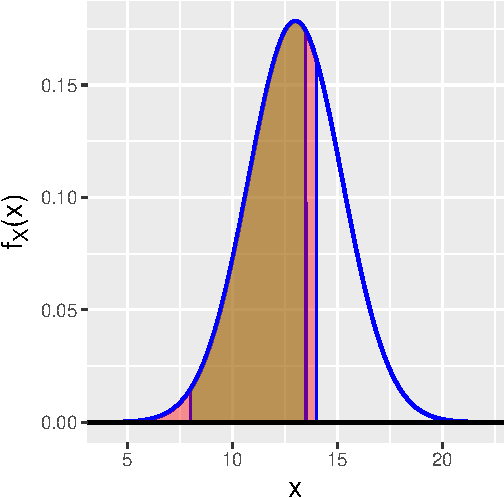
\includegraphics[keepaspectratio]{02-normal_files/figure-latex/fig-pdfcond-1.pdf}}

}

\caption{\label{fig-pdfcond}The conditional probability
\(P(8 \leq X \leq 13.5 \vert X < 14)\) is the ratio of the area of the
brown-shaded region to the area of the red-shaded region underlying the
brown-shaded region.}

\end{figure}%

\section{Normal Distribution: Cumulative Distribution
Function}\label{sec-chap2cdf}

What to take away from this section:

\begin{itemize}
\item
  The cumulative distribution function, or cdf, for a normal
  distribution contains the \emph{error function}, and so we cannot work
  with this function analytically. (Historically this motivated the
  publication and use of statistical tables.)
\item
  Foreshadowing: the non-analytic nature of the normal cdf will motivate
  us to perform any normal-related statistical inference using computer
  codes.
\end{itemize}

\smallskip\hrule

\begin{quote}
\textbf{Recall}: \emph{the cumulative distribution function, or cdf, is
another means by which to encapsulate information about a probability
distribution. For a continuous distribution, it is defined as
\(F_X(x) = \int_{y \leq x} f_Y(y) dy\), and it is defined for all values
\(x \in (-\infty,\infty)\), with \(F_X(-\infty) = 0\) and
\(F_X(\infty) = 1\).}
\end{quote}

\smallskip\hrule

The cdf for the normal distribution is the ``accumulated probability''
between \(-\infty\) and the functional input \(x\): \[
F_X(x) = \int_{-\infty}^x f_Y(y) dy = \int_{-\infty}^x \frac{1}{\sqrt{2\pi\sigma^2}} \exp\left(-\frac{(y-\mu)^2}{2\sigma^2}\right) dy \,.
\] (See Figure~\ref{fig-normcdf1}.) Recall that because \(x\) is the
upper bound of the integral, we have to replace \(x\) with some other
variable in the integrand itself. (Here we choose \(y\). The choice is
arbitrary.)

\begin{figure}

\centering{

\pandocbounded{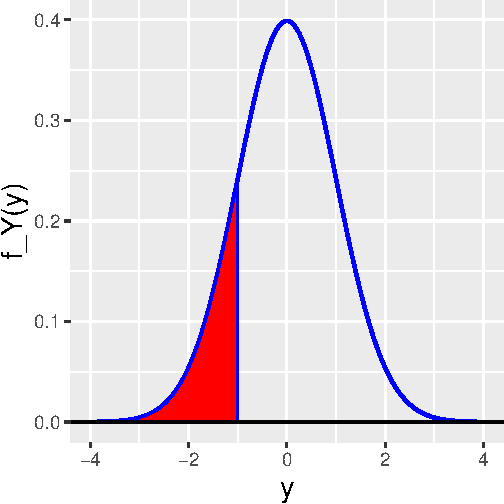
\includegraphics[keepaspectratio]{02-normal_files/figure-latex/fig-normcdf1-1.pdf}}

}

\caption{\label{fig-normcdf1}The cdf is the area of the red-shaded
polygon.}

\end{figure}%

To evaluate this integral, we again implement a variable substitution
strategy: \[
(1) ~~ t = \frac{(y-\mu)}{\sqrt{2}\sigma} ~~\implies~~ (2) ~~  dt = \frac{1}{\sqrt{2}\sigma}dy
\] and \[
(3) ~~ y = -\infty ~\implies~ t = -\infty ~~~ \mbox{and} ~~~ y = x ~\implies~ t = \frac{(x-\mu)}{\sqrt{2}\sigma} \,,
\] so \begin{align*}
F_X(x) &= \int_{-\infty}^x \frac{1}{\sqrt{2\pi\sigma^2}} \exp\left(-\frac{(y-\mu)^2}{2\sigma^2}\right) dy \\
&= \int_{-\infty}^{\frac{x-\mu}{\sqrt{2}\sigma}} \frac{1}{\sqrt{2\pi\sigma^2}} \exp(-t^2) \sqrt{2}\sigma dt = \frac{1}{\sqrt{\pi}} \int_{-\infty}^{\frac{x-\mu}{\sqrt{2}\sigma}} \exp(-t^2) dt \,.
\end{align*} The \emph{error function} is defined as \[
\mbox{erf}(z) = \frac{2}{\sqrt{\pi}} \int_0^z \exp(-t^2)dt \,,
\] which is close to, but not quite, our expression for \(F_X(x)\). (The
integrand is the same, but the bounds of integration differ.) To match
the bounds: \begin{align*}
\frac{2}{\sqrt{\pi}} \int_{-\infty}^z \exp(-t^2)dt &= \frac{2}{\sqrt{\pi}} \left( \int_{-\infty}^0 \exp(-t^2)dt + \int_0^z \exp(-t^2)dt \right) \\
&= \frac{2}{\sqrt{\pi}} \left( -\int_0^{-\infty} \exp(-t^2)dt + \int_0^z \exp(-t^2)dt \right) \\
&= -\mbox{erf}(-\infty) + \mbox{erf}(z) = \mbox{erf}(\infty) + \mbox{erf}(z) = 1 + \mbox{erf}(z) \,.
\end{align*} Here we make use of two properties of the error function:
\(\mbox{erf}(-z) = -\mbox{erf}(z)\), and \(\mbox{erf}(\infty)=1\). Thus
\[
\frac{1}{\sqrt{\pi}} \int_{-\infty}^z \exp(-t^2)dt = \frac{1}{2}[1 + \mbox{erf}(z)] \,.
\] By matching this expression with that given for \(F(x)\) above, we
see that \[
F_X(x) = \frac{1}{2}\left[1 + \mbox{erf}\left(\frac{x-\mu}{\sqrt{2}\sigma}\right)\right] \,.
\] In Figure~\ref{fig-normcdf2}, we plot \(F_X(x)\). We note that while
the error function is available to use directly in some \texttt{R}
packages, it is provided only indirectly in base-\texttt{R}, via the
\texttt{pnorm()} function. (In general, one computes cdf values for
probability distributions in \texttt{R} using functions prefixed with
\texttt{p}: \texttt{pnorm()}, \texttt{pbinom()}, \texttt{punif()}, etc.)
Examining this figure, we see that this cdf abides by the properties
listed in Section~\ref{sec-chap1cumulative}: \(F(-\infty) = 0\) and
\(F(\infty) = 1\), and it is (strictly) monotonically increasing.

\begin{figure}

\centering{

\pandocbounded{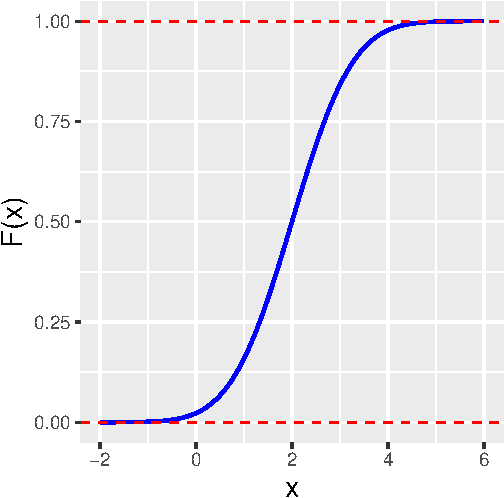
\includegraphics[keepaspectratio]{02-normal_files/figure-latex/fig-normcdf2-1.pdf}}

}

\caption{\label{fig-normcdf2}The cdf for a normal distribution with mean
0 and standard deviation 1.}

\end{figure}%

To compute the probability \(P(a < X < b)\), we make use of the cdf. (As
a reminder: if we have the cdf at our disposal and need to compute a
probability\ldots we should use it!) \begin{align*}
P(a < X < b) &= P(X < b) - P(X < a) \\
&= F(b) - F(a) = \frac{1}{2}\left[ \mbox{erf}\left(\frac{b-\mu}{\sqrt{2}\sigma}\right) - \mbox{erf}\left(\frac{a-\mu}{\sqrt{2}\sigma}\right)\right] \,,
\end{align*} which is more simply rendered in \texttt{R} as

\begin{verbatim}
pnorm(b,mean=mu,sd=sigma) - pnorm(a,mean=mu,sd=sigma)
\end{verbatim}

Let's look again at Figure~\ref{fig-normcdf1}. What if, instead of
asking the question ``what is the shaded area under the curve,'' which
is answered by integrating the normal pdf from \(-\infty\) to a
specified coordinate \(x\), we instead ask the question ``what value of
\(x\) is associated with a given area under the curve''? This is the
inverse problem, one that we can solve so long as the relationship
between \(x\) and \(F(x)\) is bijective (i.e., one-to-one):
\(x = F_X^{-1}[F_X(x)]\) for all \(x\).

\smallskip\hrule

\begin{quote}
\textbf{Recall}: \emph{an inverse cdf function \(F_X^{-1}(q)\) takes as
input a distribution quantile \(q \in [0,1]\) and returns the value of
\(x\) such that \(q = F_X(x)\).}
\end{quote}

\smallskip\hrule

Let \(q = F_X(x)\). Then, for the case of the normal cdf, we can write
that \[
x = \sqrt{2} \sigma~ \mbox{erf}^{-1}\left(2q-1\right) + \mu \,,
\] where \(\mbox{erf}^{-1}(\cdot)\) is the inverse error function. Like
the error function itself, the inverse error function is available for
use in some \texttt{R} packages, but it is most commonly accessed,
indirectly via the base-\texttt{R} function \texttt{qnorm()}. (In
general, one computes inverse cdf values for probability distributions
in \texttt{R} using functions prefixed with \texttt{q}:
\texttt{qnorm()}, \texttt{qpois()}, \texttt{qbeta()}, etc.)

\subsection{Examples}\label{examples-14}

\subsubsection{Computing Probabilities}\label{computing-probabilities-1}

\begin{quote}
We utilize the two examples provided in the last section to show how one
would compute probabilities associated with the normal pdf by hand. But
we note that a computer is still needed to derive the final numbers!
\end{quote}

\begin{quote}
\begin{enumerate}
\def\labelenumi{\arabic{enumi}.}
\tightlist
\item
  If \(X \sim \mathcal{N}(10,4)\), what is \(P(8 \leq X \leq 13.5)\)?
\end{enumerate}
\end{quote}

\begin{quote}
We have that \[
P(8 \leq X \leq 13.5) = P(X \leq 13.5) - P(X \leq 8) = F_X(13.5 \vert 10,4) - F_X(8 \vert 10,4) \,.
\] Well, this is where analytic computation ends, as we cannot evaluate
the cdfs using pen and paper. Instead, we utilize the function
\texttt{pnorm()}:
\end{quote}

\begin{Shaded}
\begin{Highlighting}[]
\FunctionTok{pnorm}\NormalTok{(}\FloatTok{13.5}\NormalTok{,}\AttributeTok{mean=}\DecValTok{10}\NormalTok{,}\AttributeTok{sd=}\FunctionTok{sqrt}\NormalTok{(}\DecValTok{4}\NormalTok{)) }\SpecialCharTok{{-}} \FunctionTok{pnorm}\NormalTok{(}\DecValTok{8}\NormalTok{,}\AttributeTok{mean=}\DecValTok{10}\NormalTok{,}\AttributeTok{sd=}\FunctionTok{sqrt}\NormalTok{(}\DecValTok{4}\NormalTok{))}
\end{Highlighting}
\end{Shaded}

\begin{verbatim}
[1] 0.8012856
\end{verbatim}

\begin{quote}
We get the same result as we got in the last section: 0.801.
\end{quote}

\begin{quote}
\begin{enumerate}
\def\labelenumi{\arabic{enumi}.}
\setcounter{enumi}{1}
\tightlist
\item
  If \(X \sim \mathcal{N}(13,5)\), what is
  \(P(8 \leq X \leq 13.5 \vert X < 14)\)?
\end{enumerate}
\end{quote}

\begin{quote}
Knowing that we cannot solve this by hand, we go directly to \texttt{R}:
\end{quote}

\begin{Shaded}
\begin{Highlighting}[]
\NormalTok{(}\FunctionTok{pnorm}\NormalTok{(}\FloatTok{13.5}\NormalTok{,}\AttributeTok{mean=}\DecValTok{13}\NormalTok{,}\AttributeTok{sd=}\FunctionTok{sqrt}\NormalTok{(}\DecValTok{5}\NormalTok{)) }\SpecialCharTok{{-}} \FunctionTok{pnorm}\NormalTok{(}\DecValTok{8}\NormalTok{,}\AttributeTok{mean=}\DecValTok{13}\NormalTok{,}\AttributeTok{sd=}\FunctionTok{sqrt}\NormalTok{(}\DecValTok{5}\NormalTok{))) }\SpecialCharTok{/} 
  \FunctionTok{pnorm}\NormalTok{(}\DecValTok{14}\NormalTok{,}\AttributeTok{mean=}\DecValTok{13}\NormalTok{,}\AttributeTok{sd=}\FunctionTok{sqrt}\NormalTok{(}\DecValTok{5}\NormalTok{))}
\end{Highlighting}
\end{Shaded}

\begin{verbatim}
[1] 0.8560226
\end{verbatim}

\begin{quote}
The answer, as before, is 0.856.
\end{quote}

\begin{quote}
But let's go ahead and add some complexity here. How would we answer the
following question?
\end{quote}

\begin{quote}
\begin{enumerate}
\def\labelenumi{\arabic{enumi}.}
\setcounter{enumi}{2}
\tightlist
\item
  If \(\mu = 20\) and \(\sigma^2 = 3\), what is the value of \(a\) such
  that \(P(20 - a \leq X \leq 20 + a) = 0.48\)?
\end{enumerate}
\end{quote}

\begin{quote}
(The first thing to thing about here is: does the value of \(\mu\)
actually matter? The answer here is no. Think about why that may be.)
\end{quote}

\begin{quote}
We have that \begin{align*}
P(20-a \leq X \leq 20+a) = 0.48 &= P(X \leq 20+a) - P(X \leq 20-a)\\
&= F_X(20+a \vert 20,3) - F_X(20-a \vert 20,3) \,.
\end{align*} Hmm\ldots we're stuck. We cannot invert this equation so as
to isolate \(a\)\ldots or can we? Remember that a normal pdf is
symmetric around the mean. Hence \[
P(X \leq 20+a) = 1 - P(X > 20+a) = 1 - P(X \leq 20-a) \,.
\] The area under the normal pdf from \(20+a\) to \(\infty\) is the same
as the area from \(-\infty\) to \(20-a\). So\ldots{} \begin{align*}
P(20-a \leq X \leq 20+a) &= 1 - F_X(20-a \vert 20,3) - F_X(20-a \vert 20,3)\\
&= 1 - 2F_X(20-a \vert 20,3) \,,
\end{align*} or \[
F_X(20-a \vert 20,3) = \frac{1}{2}[1 - P(20-a \leq X \leq 20+a)] = \frac{1}{2} 0.52 = 0.26 \,.
\] Now, we invert the cdf and rearrange terms to get: \[
a = 20 - F_X^{-1}(0.26 \vert 20,3) \,,
\] and once again, we transition to \texttt{R}:
\end{quote}

\begin{Shaded}
\begin{Highlighting}[]
\NormalTok{a }\OtherTok{\textless{}{-}} \DecValTok{20} \SpecialCharTok{{-}} \FunctionTok{qnorm}\NormalTok{(}\FloatTok{0.26}\NormalTok{,}\AttributeTok{mean=}\DecValTok{20}\NormalTok{,}\AttributeTok{sd=}\FunctionTok{sqrt}\NormalTok{(}\DecValTok{3}\NormalTok{))}
\end{Highlighting}
\end{Shaded}

\begin{quote}
The result is \(a = 1.114\), i.e.,
\(P(18.886 \leq X \leq 21.114) = 0.48\).
\end{quote}

\begin{quote}
The reader might quibble with our assertion that \(\mu\) doesn't matter
here, because, after all, the value of \(\mu\) appears in the final
code. However, if we changed both values of 20 to some other, arbitrary
value, we would derive the same value for \(a\).
\end{quote}

\subsubsection{Visualization}\label{visualization}

\begin{quote}
Let's say we want to make a figure like that in
Figure~\ref{fig-normcdf1}, where we are given that our normal
distribution has mean \(\mu = 10\) and variance \(\sigma^2 = 4\), and we
want to overlay the shaded region associated with \(F_X(9)\). How do we
do this?
\end{quote}

\begin{quote}
The first step is to determine the population standard deviation. Here,
that would be \(\sigma = \sqrt{4} = 2\).
\end{quote}

\begin{quote}
The second step is to determine an appropriate range of values of \(x\)
over which to plot the cdf. Here we will assume that \(\mu - 4\sigma\)
to \(\mu + 4\sigma\) is sufficient; this corresponds to \(x = 2\) to
\(x = 18\).
\end{quote}

\begin{quote}
The third step is to code. The result of our coding is shown in
Figure~\ref{fig-normviz}.
\end{quote}

\begin{figure}

\centering{

\pandocbounded{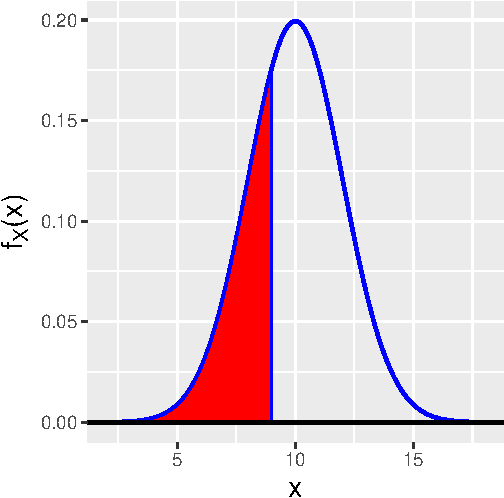
\includegraphics[keepaspectratio]{02-normal_files/figure-latex/fig-normviz-1.pdf}}

}

\caption{\label{fig-normviz}The cumulative distribution function is the
area of the red-shaded region.}

\end{figure}%

For the polygon, the first \((x,y)\) pair is \((9,0)\), the second is
\((2,0)\) (where \(x = 2\) is the lower limit of the plot\ldots there is
no need to take the polygon further ``to the left''), and the next set
are \((x,f_X(x))\) for all \(x\) values \(\leq 9\). The last point is
the first point: this closes the polygon.

\section{Method of Moment-Generating
Functions}\label{sec-chap2methodmgf}

What to take away from this section:

\begin{itemize}
\item
  A \emph{moment-generating function} or \emph{mgf} is, like a
  probability mass or density function or like a cumulative distribution
  function, a means by which to encapsulate the information contained in
  a probability distribution.
\item
  An mgf is derived by computing the expected value \(E[e^{tX}]\).
\item
  Our primary use for an mgf is as a tool that allows us to attempt to
  identify the sampling distributions of statistics, such as the sample
  mean or the sample sum\ldots this is the \emph{method of
  moment-generating functions}.
\item
  Foreshadowing: in the next section, we will use the method of mgfs to
  determine the distributions associated with linear functions of
  normally distributed random variables.
\end{itemize}

For previous material on sampling distributions, see
Section~\ref{sec-chap1sampdist}.

In Section~\ref{sec-chap1expected}, we learned that if we linearly
transform a random variable, i.e., if we define a new random variable
\(Y = \sum_{i=1}^n a_i X_i + b\), where \(\{a_1,\ldots,a_n\}\) and \(b\)
are constants, then \[
E[Y] = E\left[\sum_{i=1}^n a_i X_i + b\right] = b + \sum_{i=1}^n a_i E[X_i] \,.
\] Furthermore, if we assume that the \(X_i\)'s are independent random
variables, then the variance of \(Y\) is \[
V[Y] = V\left[\sum_{i=1}^n a_i X_i + b\right] = \sum_{i=1}^n a_i^2 V[X_i] \,.
\] (Because the \(X_i\)'s are independent, we do not need to take into
account any covariance, or linear dependence, between the \(X_i\)'s,
simplifying the equation for \(V[Y]\). We discuss how covariance is
taken into account in Section~\ref{sec-chap6covariance}.) So we know
where \(Y\) is centered and we know how ``wide'' it is. However, we
don't yet know the shape of the distribution for \(Y\), i.e., we don't
yet know \(f_Y(y)\). To show how we might derive the distribution, we
introduce a new concept, that of the \emph{moment-generating function},
or \emph{mgf}.

\subsection{Moment-Generating Functions}\label{sec-chap2mgf}

In Section~\ref{sec-chap1expected}, we briefly introduced the concept of
distribution moments, i.e., the expected values \(E[X^k]\) and
\(E[(X-\mu)^k]\). The moments of a given probability distribution are
unique, and can often (but not always) be neatly encapsulated in a
single mathematical expression: the moment-generating function (or mgf).
To derive an mgf for a given distribution, we invoke the Law of the
Unconscious Statistician: \begin{align*}
m_X(t) = E[e^{tX}] &= \int_x e^{tX} f_X(x) \\
&= \int_x \left[1 + tx + \frac{t^2}{2!}x^2 + \cdots \right] f_X(x) \\
&= \int_x \left[ f_X(x) + t x f_X(x) + \frac{t^2}{2!} x^2 f_X(x) + \cdots \right] \\
&= \int_x f_X(x) + t \int_x x f_X(x) + \frac{t^2}{2!} \int_x x^2 f_X(x) + \cdots \\
&= 1 + t E[X] + \frac{t^2}{2!} E[X^2] + \cdots \,.
\end{align*} (Note that what statisticians call a moment-generating
function is what mathematicians would call a \emph{Laplace tranform}.)
An mgf only exists for a particular distribution if there is a constant
\(b\) such that \(m_X(t)\) is finite for \(\vert t \vert < b\). (This is
a detail that we will not concern ourselves with here, i.e., we will
assume that the expressions we derive for \(E[e^{tX}]\) are valid
expressions.) An example of a distribution for which the mgf does not
exist is the Cauchy distribution.

Moment-generating functions are called such because, as one might guess,
they generate moments (via differentiation): \begin{align*}
\left.\frac{d^k m_X(t)}{dt^k}\right|_{t=0} &= \frac{d^k}{dt^k} \left. \left[1 + t E[X] + \frac{t^2}{2!} E[X^2] + \cdots \right]\right|_{t=0}\\
&= \left. \left[E[X^k] + tE[X^{k+1}] + \cdots\right] \right|_{t=0} = E[X^k] \,.
\end{align*} The \(k^{\mathrm{th}}\) derivative of an mgf, with \(t\)
set to zero, yields the \(k^{\mathrm{th}}\) moment \(E[X^k]\).

\subsection{Sampling Distributions via the Method of Moment-Generating
Functions}\label{sec-chap2method}

But, the reader may ask, why are mgfs important here, in the context of
normal random variables? We already know all the moments of this
distribution that we care to know: they are written down (or can be
derived directly via the integration of \(x^k f_X(x)\)). The answer is
that a remarkably useful property of mgfs is the following: if
\(Y = b + \sum_{i=1}^n a_i X_i\), where the \(X_i\)'s are independent
random variables sampled according to a distribution whose mgf exists,
then \[
m_Y(t) = e^{bt} m_{X_1}(a_1 t) m_{X_2}(a_2 t) \cdots m_{X_n}(a_n t) = e^{bt} \prod_{i=1}^n m_{X_i}(a_i t) \,,
\] where \(m_{X_i}(\cdot)\) is the moment-generating function for the
random variable \(X_i\). An mgf is typically written as a function of
\(t\); the notation \(m_{X_i}(a_it)\) simply means that when we evaluate
the above equation, wherever there is a \(t\), we plug in \(a_it\).
Here's the key point: \emph{if we recognize the form of \(m_Y(t)\) as
matching that of the mgf for a given distribution, then we know the
sampling distribution for \(Y\)}.

Below, we show how the method of moment-generating functions allows us
to derive sampling distributions for linearly transformed normal random
variables.

For more on how we derive sampling distributions in practice, go to
Section~\ref{sec-chap2linear}, Section~\ref{sec-chap2standard},
Section~\ref{sec-chap3linear}, Section~\ref{sec-chap4linear}, and
Section~\ref{sec-chap5linear}. What happens if we cannot derive a
sampling distribution? We can simulate or utilize the bootstrap
algorithm. See, e.g., Section~\ref{sec-chap4bootstrap}.

\subsection{Examples}\label{examples-15}

\subsubsection{MGF: Probability Mass
Function}\label{mgf-probability-mass-function}

\begin{quote}
Let's assume that we sample data from the following pmf:
\end{quote}

{\def\LTcaptype{none} % do not increment counter
\begin{longtable}[]{@{}cc@{}}
\toprule\noalign{}
\(x\) & \(p_X(x)\) \\
\midrule\noalign{}
\endhead
\bottomrule\noalign{}
\endlastfoot
0 & 0.2 \\
1 & 0.3 \\
2 & 0.5 \\
\end{longtable}
}

\begin{quote}
What is the mgf for this distribution? What is its expected value? If we
sample two data, \(X_1\) and \(X_2\), independently from this
distribution, what is the mgf of the sampling distribution for
\(Y = 2X_1 - X_2\)?
\end{quote}

\begin{quote}
To derive the mgf, we compute \(E[e^{tX}]\): \begin{align*}
m_X(t) &= E[e^{tX}] = \sum_x e^{tx} p_X(x) = 1 \cdot 0.2 + e^t \cdot 0.3 + e^{2t} \cdot 0.5\\
&= 0.2 + 0.3 e^t + 0.5 e^{2t} \,.
\end{align*} This cannot be simplified, and thus this is the final
answer. As far as the expected value is concerned: we could simply
compute \(E[X] = \sum_x x p_X(x)\), but since we have the mgf now, we
can use it too: \[
E[X] = \left.\frac{d}{dt}m_X(t)\right|_{t=0} = \left. (0.3 e^t + e^{2t})\right|_{t=0} = 0.3 + 1 = 1.3 \,.
\] As for the linear function \(Y = 2X_1 - X_2\): if we refer back to
the equation above, we see that \begin{align*}
m_Y(t) &= e^{bt} m_{X_1}(a_1t) m_{X_2}(a_2t) = e^{0t} m_{X_1}(2t) m_{X_2}(-1t) \\
&= \left(0.2 + 0.3e^{2t} + 0.5e^{4t}\right) \left(0.2 + 0.3e^{-t} + 0.5e^{-2t}\right) \\
&= 0.19 + 0.10 e^{-2t} + 0.06 e^{-t} + 0.09 e^t + 0.31 e^{2t} + 0.15 e^{3t} + 0.10 e^{4t} \,.
\end{align*}
\end{quote}

\subsubsection{MGF: Probability Density
Function}\label{mgf-probability-density-function}

\begin{quote}
Let's assume that we now sample data from the following pdf: \[
f_X(x) = \frac{1}{\theta} e^{-x/\theta} \,,
\] where \(x \geq 0\) and \(\theta > 0\). What is the mgf of this
distribution? If we sample two data, \(X_1\) and \(X_2\), independently
from this distribution, what is the mgf of the sampling distribution for
\(Y = X_1 + X_2\)?
\end{quote}

\begin{quote}
To derive the mgf, we compute \(E[e^{tX}]\): \begin{align*}
E[e^{tX}] &= \int_0^\infty e^{tx} \frac{1}{\theta} e^{-x/\theta} dx = \frac{1}{\theta} \int_0^\infty e^{-x\left(\frac{1}{\theta}-t\right)} dx \\
&= \frac{1}{\theta} \int_0^\infty e^{-x/\theta'} dx = \frac{\theta'}{\theta} = \frac{1}{\theta} \frac{1}{(1/\theta - t)} = \frac{1}{(1-\theta t)} = (1-\theta t)^{-1} \,.
\end{align*} The expected value of this distribution can be computed via
the integral \(\int_x x f_X(x) dx\), but again, as we now have the mgf,
\[
E[X] = \left.\frac{d}{dt}m_X(t)\right|_{t=0} = \left. -(1-\theta t)^{-2} (-\theta)\right|_{t=0} = \theta \,.
\] As for the linear function \(Y = X_1 + X_2\): if we refer back to the
equation above, we see that \begin{align*}
m_Y(t) &= e^{bt} m_{X_1}(a_1t) m_{X_2}(a_2t) = e^{0t} m_{X_1}(t) m_{X_2}(t) \\
&= (1-\theta t)^{-1} (1-\theta t)^{-1} = (1 - \theta t)^{-2} \,.
\end{align*} While the reader would not know this yet, this is the mgf
for a gamma distribution with shape parameter \(a = 2\) and scale
parameter \(b = \theta\). We will officially introduce the gamma
distribution in Section~\ref{sec-chap4gamma}.
\end{quote}

\subsubsection{MGF: Normal Distribution}\label{mgf-normal-distribution}

\begin{quote}
The moment-generating function for a normal distribution is
\begin{align*}
m_X(t) &= E[e^{tX}] = \int_{-\infty}^\infty e^{tx} \frac{1}{\sqrt{2\pi \sigma^2}} \exp\left(-\frac{(x-\mu)^2}{2\sigma^2}\right) dx \\
&= \frac{1}{\sqrt{2\pi \sigma^2}} \int_{-\infty}^\infty \exp\left(-\frac{x^2}{2\sigma^2}\right) \exp\left(x(\frac{\mu}{\sigma^2}+t)\right) \exp\left(-\frac{\mu^2}{2\sigma^2}\right) dx \\
&= \frac{1}{\sqrt{2\pi \sigma^2}} \int_{-\infty}^\infty \exp\left(-\frac{x^2}{2\sigma^2}\right) \exp\left(\frac{x\mu'}{\sigma^2}\right) \exp\left(-\frac{\mu^2}{2\sigma^2}\right) dx \,,
\end{align*} where \(\mu' = \mu + t\sigma^2\). To solve this integral,
we utilize the method of ``completing the square.'' We know that \[
(x - \mu')^2 = x^2 - 2x\mu' + (\mu')^2 \,,
\] so we will introduce a new term that is equal to 1 into the
integrand: \[
\exp\left(-\frac{(\mu')^2}{2\sigma^2}\right) \exp\left(\frac{(\mu')^2}{2\sigma^2}\right) \,.
\] Now we have that
\end{quote}

\begin{align*}
m_X(t) &= \frac{1}{\sqrt{2\pi \sigma^2}} \int_{-\infty}^\infty \exp\left(-\frac{x^2}{2\sigma^2}\right) \exp\left(\frac{x\mu'}{\sigma^2}\right) \exp\left(-\frac{(\mu')^2}{2\sigma^2}\right) \exp\left(\frac{(\mu')^2}{2\sigma^2}\right) \exp\left(-\frac{\mu^2}{2\sigma^2}\right) dx \\
&= \frac{1}{\sqrt{2\pi \sigma^2}} \exp\left(\frac{(\mu')^2}{2\sigma^2}\right) \exp\left(-\frac{\mu^2}{2\sigma^2}\right) \int_{-\infty}^\infty \exp\left(-\frac{x^2}{2\sigma^2}\right) \exp\left(\frac{2x\mu'}{2\sigma^2}\right) \exp\left(-\frac{(\mu')^2}{2\sigma^2}\right) dx \\
&= \exp\left(\frac{(\mu')^2}{2\sigma^2}\right) \exp\left(-\frac{\mu^2}{2\sigma^2}\right) \int_{-\infty}^\infty \frac{1}{\sqrt{2\pi \sigma^2}} \exp\left(-\frac{(x-\mu')^2}{2\sigma^2}\right) dx \\
&= \exp\left(\frac{(\mu')^2}{2\sigma^2}\right) \exp\left(-\frac{\mu^2}{2\sigma^2}\right) \,.
\end{align*}

\begin{quote}
The integral disappears because it is the integral of the pdf for a
\(\mathcal{N}(\mu',\sigma^2)\) distribution over its entire domain; that
integral is 1. Continuing\ldots{}
\end{quote}

\begin{align*}
m_X(t) &= \frac{1}{\sqrt{2\pi \sigma^2}} \int_{-\infty}^\infty \exp\left(-\frac{x^2}{2\sigma^2}\right) \exp\left(\frac{x\mu'}{\sigma^2}\right) \exp\left(-\frac{(\mu')^2}{2\sigma^2}\right) \exp\left(\frac{(\mu')^2}{2\sigma^2}\right) \exp\left(-\frac{\mu^2}{2\sigma^2}\right) dx \\
&= \frac{1}{\sqrt{2\pi \sigma^2}} \exp\left(\frac{(\mu')^2}{2\sigma^2}\right) \exp\left(-\frac{\mu^2}{2\sigma^2}\right) \int_{-\infty}^\infty \exp\left(-\frac{x^2}{2\sigma^2}\right) \exp\left(\frac{2x\mu'}{2\sigma^2}\right) \exp\left(-\frac{(\mu')^2}{2\sigma^2}\right) dx \\
&= \exp\left(\frac{(\mu')^2}{2\sigma^2}\right) \exp\left(-\frac{\mu^2}{2\sigma^2}\right) \int_{-\infty}^\infty \frac{1}{\sqrt{2\pi \sigma^2}} \exp\left(-\frac{(x-\mu')^2}{2\sigma^2}\right) dx \\
&= \exp\left(\frac{(\mu')^2}{2\sigma^2}\right) \exp\left(-\frac{\mu^2}{2\sigma^2}\right) = \exp\left(\frac{\mu^2}{2\sigma^2}\right) \exp\left(\frac{2\mu\sigma^2t}{2\sigma^2}\right) \exp\left(\frac{\sigma^4t^2}{2\sigma^2}\right) \exp\left(-\frac{\mu^2}{2\sigma^2}\right) \\
&= \exp\left(\mu t\right) \exp\left(\frac{\sigma^2t^2}{2}\right) = \exp\left(\mu t + \frac{\sigma^2t^2}{2} \right) \,.
\end{align*}

\begin{quote}
We will utilize this function in the next section below to derive the
mgfs for linear functions of normal random variables.
\end{quote}

\section{Normal Distribution: Linear Functions of Random
Variables}\label{sec-chap2linear}

What to take away from this section:

\begin{itemize}
\item
  The \emph{method of moment-generating functions} allows us to
  determine that\ldots{}

  \begin{itemize}
  \item
    the sum of \(n\) independent but not necessarily identically
    distributed normal random variables is itself normally distributed;
    and
  \item
    the mean of \(n\) iid normal random variables is itself normally
    distributed.
  \end{itemize}
\item
  Foreshadowing: these results will allow us to make statistical
  inferences about the normal population mean \(\mu\), given \(n\) iid
  normal random variables, when the population variance \(\sigma^2\) is
  known.
\end{itemize}

For previous material on sampling distributions, see
Section~\ref{sec-chap2methodmgf}.

Suppose we are given \(n\) normal random variables
\(\{X_1,\ldots,X_n\}\), which are independent (but, for now, not
necessarily identically distributed), and we wish to determine the
distribution of the sum \(Y = b + \sum_{i=1}^n a_i X_i\). As shown
above, the moment-generating function for any one of the random
variables is \[
m_{X_i}(t) = \exp\left(\mu_i t + \sigma_i^2\frac{t^2}{2} \right) \,.
\] Thus, by the method of moment-generating functions, \begin{align*}
m_Y(t) &= \exp(bt) \prod_{i=1}^n m_{X_i}(a_it) \\
&= \exp(bt) \exp\left(\mu_1a_1t+a_1^2\sigma_1^2\frac{t^2}{2}\right) \cdot \cdots \cdot \exp\left(\mu_na_nt+a_n^2\sigma_n^2\frac{t^2}{2}\right) \\
&= \exp\left[ (b+a_1\mu_1+\cdots+a_n\mu_n)t + \left(a_1^2\sigma_1^2 + \cdots + a_n^2\sigma_n^2\right)\frac{t^2}{2} \right] \\
&= \exp\left[ \left(b+\sum_{i=1}^n a_i\mu_i\right)t + \left(\sum_{i=1}^n a_i^2\sigma_i^2\right)\frac{t^2}{2} \right] \,.
\end{align*} The result retains the functional form of a normal mgf, and
thus we conclude that \(Y\) itself is a normally distributed random
variable, with mean \(b+\sum_{i=1}^n a_i\mu_i\) and variance
\(\sum_{i=1}^n a_i^2\sigma_i^2\): \[
Y \sim \mathcal{N}\left(b+\sum_{i=1}^n a_i\mu_i,\sum_{i=1}^n a_i^2\sigma_i^2\right) \,.
\] If the data are identically distributed, then we can re-express the
above as \[
Y \sim \mathcal{N}\left(b+(\sum_{i=1}^n a_i)\mu,(\sum_{i=1}^n a_i^2)\sigma^2\right) \,.
\] We will utilize this second result extensively\ldots and we will
start by looking at the sample mean.

If \(Y = \bar{X} = (\sum_{i=1}^n X_i)/n\), then \(b = 0\) and each of
the \(a_i\)'s is \(1/n\). Thus \[
Y = \bar{X} \sim \mathcal{N}\left(\mu \sum_{i=1}^n \frac{1}{n},\sigma^2 \sum_{i=1}^n \frac{1}{n^2} \right) ~~~~~~\mbox{or}~~~~~~ \bar{X} \sim \mathcal{N}\left(\mu,\frac{\sigma^2}{n}\right) \,.
\] We see that the sample mean that we observe in any given experiment
is drawn according to a normal distribution that is centered on the true
mean and that has a width that goes to zero as \(n \rightarrow \infty\).

\subsection{Examples}\label{examples-16}

\subsubsection{Computing Probabilities}\label{computing-probabilities-2}

\begin{quote}
Let \(X_1 \sim \mathcal{N}(10,4^2)\) and \(X_2 \sim \mathcal{N}(8,2^2)\)
be two independent random variables, and let \(Y = X_1 - X_2\). What is
\(P(0 \leq Y \leq 2)\)?
\end{quote}

\begin{quote}
From above, we see that \begin{align*}
Y &\sim \mathcal{N}\left(b + \sum_{i=1}^n a_i \mu_i,\sum_{i=1}^n a_i^2 \sigma_i^2\right)\\
\Rightarrow ~~~ Y &\sim \mathcal{N}\left(10-8,4^2+2^2\right)\\
\Rightarrow ~~~ Y &\sim \mathcal{N}(2,20) \,.
\end{align*} Thus the probability we seek is \[
P(0 \leq Y \leq 2) = P(Y \leq 2) - P(Y \leq 0) = F_Y(2) - F_Y(0) \,,
\] or
\end{quote}

\begin{Shaded}
\begin{Highlighting}[]
\FunctionTok{pnorm}\NormalTok{(}\DecValTok{2}\NormalTok{, }\AttributeTok{mean =} \DecValTok{2}\NormalTok{, }\AttributeTok{sd =} \FunctionTok{sqrt}\NormalTok{(}\DecValTok{20}\NormalTok{)) }\SpecialCharTok{{-}} \FunctionTok{pnorm}\NormalTok{(}\DecValTok{0}\NormalTok{, }\AttributeTok{mean =} \DecValTok{2}\NormalTok{, }\AttributeTok{sd =} \FunctionTok{sqrt}\NormalTok{(}\DecValTok{20}\NormalTok{))}
\end{Highlighting}
\end{Shaded}

\begin{verbatim}
[1] 0.1726396
\end{verbatim}

\begin{quote}
There is a 17.3\% chance that when we sample \(X_1\) and \(X_2\), the
difference \(X_1 - X_2\) has a value between 0 and 2.
\end{quote}

\subsubsection{Sample Sum}\label{sample-sum}

\begin{quote}
If \(Y = X_+ = \sum_{i=1}^n X_i)\), then we know that \(b = 0\) and each
of the \(a_i\)'s is \(1\). Thus \[
Y = X_+ \sim \mathcal{N}\left(\mu (\sum_{i=1}^n 1),\sigma^2 (\sum_{i=1}^n 1^2) \right) ~~~~~~\mbox{or}~~~~~~ X_+ \sim \mathcal{N}\left(n\mu,n\sigma^2\right) \,.
\]
\end{quote}

\section{Normal Distribution: Standardization}\label{sec-chap2standard}

What to take away from this section:

\begin{itemize}
\item
  The \emph{method of moment-generating functions} allows us to
  determine that\ldots{}

  \begin{itemize}
  \tightlist
  \item
    if \(X\) is a normal random variable, the \emph{standardized}
    quantity \(Z = (X-\mu)/\sigma\) is distributed according to a
    \emph{standard normal distribution} (i.e., a normal distribution for
    which \(\mu = 0\) and \(\sigma^2 = 1\)).
  \end{itemize}
\item
  Use of the standard normal distribution, the basis of the so-called
  \(z\)-tables of standard statistical textbooks, has now become largely
  superseded as we can use computers to work with any normal
  distribution directly.
\end{itemize}

For previous material on sampling distributions, see
Section~\ref{sec-chap2methodmgf}.

To standardize a random variable that is sampled according to \emph{any}
distribution, we subtract off its expected value and then divide by its
standard deviation: \[
Z = \frac{X - E[X]}{\sqrt{V[X]}} \,.
\] If \(X \sim \mathcal{N}(\mu,\sigma^2)\), and thus if
\(Z = (X-\mu)/\sigma\), what is \(f_Z(z)\)? Going back to the result we
wrote down above, \[
Y \sim \mathcal{N}\left(b+(\sum_{i=1}^n a_i)\mu,(\sum_{i=1}^n a_i^2)\sigma^2\right) \,.
\] Here, \(Y = Z\), with \(n=1\), \(a_1 = 1/\sigma\), and
\(b = -\mu/\sigma\). Thus \[
Z \sim \mathcal{N}\left(-\frac{\mu}{\sigma}+\frac{1}{\sigma}\mu,\frac{1}{\sigma^2}\sigma^2\right) ~~~~~~\mbox{or}~~~~~~ Z \sim \mathcal{N}\left(0,1\right) \,.
\] \(Z\) is a \emph{standard normal} random variable. Its probability
density function is \[
f_Z(z) = \frac{1}{\sqrt{2\pi}} \exp\left(-\frac{z^2}{2}\right) ~~~~ z \in (-\infty,\infty) \,,
\] while its cumulative distribution function is \[
F_Z(z) = \Phi(z) = \frac{1}{2}\left[1 + \mbox{erf}\left(\frac{z}{\sqrt{2}}\right)\right] \,.
\] By historical convention, the cdf of the standard normal distribution
is denoted \(\Phi(z)\) (``phi'' of z, pronounced ``fye'') rather than
\(F_Z(z)\).

Statisticians often standardize normally distributed random variables
and perform probability calculations using the standard normal.
\textbf{Strictly speaking, standardization is unnecessary in the age of
computers}, but in the pre-computer era standardization greatly
simplified probability calculations since all one needed was a single
table of values of \(\Phi(z)\): \[
P(a \leq Z \leq b) = \Phi(b) - \Phi(a) \,.
\] One can argue that standardization is useful for mental calculation:
for instance, mentally computing an approximate value for
\(P(6 < X < 12)\) when \(X \sim \mathcal{N}(9,9)\) can be quite a bit
more taxing than if we were to work with the equivalent expression
\(P(-1 < Z < 1)\), which a skilled practitioner would know right away to
be \(\approx\) 0.68.

{\def\LTcaptype{none} % do not increment counter
\begin{longtable}[]{@{}
  >{\raggedright\arraybackslash}p{(\linewidth - 12\tabcolsep) * \real{0.1429}}
  >{\raggedright\arraybackslash}p{(\linewidth - 12\tabcolsep) * \real{0.1429}}
  >{\raggedright\arraybackslash}p{(\linewidth - 12\tabcolsep) * \real{0.1429}}
  >{\raggedright\arraybackslash}p{(\linewidth - 12\tabcolsep) * \real{0.1429}}
  >{\raggedright\arraybackslash}p{(\linewidth - 12\tabcolsep) * \real{0.1429}}
  >{\raggedright\arraybackslash}p{(\linewidth - 12\tabcolsep) * \real{0.1429}}
  >{\raggedright\arraybackslash}p{(\linewidth - 12\tabcolsep) * \real{0.1429}}@{}}
\toprule\noalign{}
\begin{minipage}[b]{\linewidth}\raggedright
\((a,b)\)
\end{minipage} & \begin{minipage}[b]{\linewidth}\raggedright
\(\pm\) 1
\end{minipage} & \begin{minipage}[b]{\linewidth}\raggedright
\(\pm\) 2
\end{minipage} & \begin{minipage}[b]{\linewidth}\raggedright
\(\pm\) 3
\end{minipage} & \begin{minipage}[b]{\linewidth}\raggedright
\(\pm\) 1.645
\end{minipage} & \begin{minipage}[b]{\linewidth}\raggedright
\(\pm\) 1.960
\end{minipage} & \begin{minipage}[b]{\linewidth}\raggedright
\(\pm\) 2.576
\end{minipage} \\
\midrule\noalign{}
\endhead
\bottomrule\noalign{}
\endlastfoot
\(P(a \leq Z \leq b)\) & 0.6837 & 0.9544 & 0.9973 & 0.90 & 0.95 &
0.99 \\
\end{longtable}
}

\subsection{Example}\label{example-1}

\subsubsection{Computing Probabilities}\label{computing-probabilities-3}

\begin{quote}
Here we will reexamine the three examples that we worked through above
in the section in which we introduce the normal cumulative distribution
function; here, we will utilize standardization. Note: the final results
will all be the same!
\end{quote}

\begin{quote}
\begin{enumerate}
\def\labelenumi{\arabic{enumi}.}
\tightlist
\item
  If \(X \sim \mathcal{N}(10,4)\), what is \(P(8 \leq X \leq 13.5)\)?
\end{enumerate}

We standardize \(X\): \(Z = (X-\mu)/\sigma = (X-10)/2\). Hence the
bounds of integration are \((8-10)/2 = -1\) and \((13.5-10)/2 = 1.75\),
and the probability we seek is \[
P(-1 \leq Z \leq 1.75) = \Phi(1.75) - \Phi(-1) \,.
\] To compute the final number, we utilize \texttt{pnorm()} with its
default values of \texttt{mean\ =\ 0} and \texttt{sd\ =\ 1}:
\end{quote}

\begin{Shaded}
\begin{Highlighting}[]
\FunctionTok{pnorm}\NormalTok{(}\FloatTok{1.75}\NormalTok{) }\SpecialCharTok{{-}} \FunctionTok{pnorm}\NormalTok{(}\SpecialCharTok{{-}}\DecValTok{1}\NormalTok{)}
\end{Highlighting}
\end{Shaded}

\begin{verbatim}
[1] 0.8012856
\end{verbatim}

\begin{quote}
The probability is 0.801.
\end{quote}

\begin{quote}
\begin{enumerate}
\def\labelenumi{\arabic{enumi}.}
\setcounter{enumi}{1}
\tightlist
\item
  If \(X \sim \mathcal{N}(13,5)\), what is
  \(P(8 \leq X \leq 13.5 \vert X < 14)\)?
\end{enumerate}

The integral bounds are \((8-13)/\sqrt{5} = -\sqrt{5}\) and
\((13.5-13)/\sqrt{5} = \sqrt{5}/10\) in the numerator, and \(-\infty\)
and \((14-13/\sqrt{5} = \sqrt{5}/5\) in the denominator. In \texttt{R}:
\end{quote}

\begin{Shaded}
\begin{Highlighting}[]
\NormalTok{(}\FunctionTok{pnorm}\NormalTok{(}\FunctionTok{sqrt}\NormalTok{(}\DecValTok{5}\NormalTok{) }\SpecialCharTok{/} \DecValTok{10}\NormalTok{) }\SpecialCharTok{{-}} \FunctionTok{pnorm}\NormalTok{(}\SpecialCharTok{{-}}\FunctionTok{sqrt}\NormalTok{(}\DecValTok{5}\NormalTok{))) }\SpecialCharTok{/} \FunctionTok{pnorm}\NormalTok{(}\FunctionTok{sqrt}\NormalTok{(}\DecValTok{5}\NormalTok{) }\SpecialCharTok{/} \DecValTok{5}\NormalTok{)}
\end{Highlighting}
\end{Shaded}

\begin{verbatim}
[1] 0.8560226
\end{verbatim}

\begin{quote}
The probability is 0.856.
\end{quote}

\begin{quote}
\begin{enumerate}
\def\labelenumi{\arabic{enumi}.}
\setcounter{enumi}{2}
\tightlist
\item
  If \(\mu = 20\) and \(\sigma^2 = 3\), what is the value of \(a\) such
  that \(P(20-a \leq X \leq 20+a) = 0.48\)?
\end{enumerate}
\end{quote}

\begin{quote}
Here, \begin{align*}
P(20-a \leq X \leq 20+a) &= P\left( \frac{20-a-20}{\sqrt{3}} \leq \frac{X - 20}{\sqrt{3}} \leq \frac{20+a-20}{\sqrt{3}}\right)\\
&= P\left(-\frac{a}{\sqrt{3}} \leq Z \leq \frac{a}{\sqrt{3}} \right) \,,
\end{align*} and we utilize the symmetry of the standard normal around
zero to write \[
P\left(-\frac{a}{\sqrt{3}} \leq Z \leq \frac{a}{\sqrt{3}} \right) = 1 - 2P\left(Z \leq -\frac{a}{\sqrt{3}}\right) = 1 - 2\Phi\left(-\frac{a}{\sqrt{3}}\right) \,.
\] Thus \begin{align*}
1 - 2\Phi\left(-\frac{a}{\sqrt{3}}\right) = 0.48 ~~~ &\Rightarrow ~~~ \Phi\left(-\frac{a}{\sqrt{3}}\right) = 0.26\\
&\Rightarrow ~~~ -\frac{a}{\sqrt{3}} = \Phi^{-1}(0.26) = -0.64 \,,
\end{align*} and thus \(a = 1.114\). (Note that we numerically evaluate
\(\Phi^{-1}(0.26)\) using \texttt{qnorm(0.26)}).
\end{quote}

\section{The Central Limit Theorem}\label{sec-chap2clt}

What to take away from this section:

\begin{itemize}
\item
  If \(\{X_1,\ldots,X_n\}\) are \(n\) iid data sampled according to the
  not-normal distribution \(P\), then if \(n\) is large (by convention,
  \(> 30\)), we can assume that the sample mean \(\bar{X}\) is (at least
  approximately) distributed according to a normal distribution with
  mean \(\mu\) and variance \(S^2/n\) (or \(\sigma^2/n\) if \(\sigma^2\)
  is known).
\item
  Foreshadowing: this result gives us the ability to derive at least
  approximate inferences about a population mean \(\mu\) when we cannot
  determine the exact sampling distribution for \(\bar{X}\).
\end{itemize}

Thus far in this chapter, we have assumed that we have sampled
individual data from normal distributions. While we have been able to
illustrate many concepts related to probability and statistical
inference in this setting, the reader may feel that this is unduly
limiting: what if the data we sample are not normally distributed? While
we do examine the world beyond normality in future chapters, there is
one major concept we can discuss now: the idea that \emph{statistics}
computed using non-normal data can themselves have sampling
distributions that are at least approximately normal. This is big: it
means that, e.g., we can utilize the same machinery for deriving
normal-based confidence intervals and for conducting normal-based
hypothesis tests, machinery that we outline below, to generate
inferences for these (approximately) normally distributed statistics.

The \emph{central limit theorem}, or \emph{CLT}, is one of the most
important probability theorems, if not the most important. It states
that if we have \(n\) iid random variables \(\{X_1,\ldots,X_n\}\) with
mean \(E[X_i] = \mu\) and finite variance
\(V[X_i] = \sigma^2 < \infty\), and if \(n\) is sufficiently large, then
\(\bar{X}\) is approximately normally distributed, and
\((\bar{X}-\mu)/(\sigma/\sqrt{n})\) is approximately standard normally
distributed: \[
\lim_{n \rightarrow \infty} P\left(\frac{\bar{X}-\mu}{\sigma/\sqrt{n}} \leq z \right) = \Phi(z) \,.
\] In other words, \[
{\bar X} \overset{d}{\rightarrow} Y \sim \mathcal{N}\left(\mu,\frac{\sigma^2}{n}\right) ~~\mbox{or}~~ \frac{\sqrt{n}(\bar{X}-\mu)}{\sigma} \overset{d}{\rightarrow} Z \sim \mathcal{N}(0,1) \,.
\] The limit notation to the left above is to be read as ``\(\bar{X}\)
\emph{converges in distribution} to normally distributed random
variable,'' i.e., the shape of the probability density function for
\(\bar{X}\) tends to that of a normal distribution as
\(n \rightarrow \infty\). Note that as an alternative to the sample
mean, we can also work with the sample sum: \[
X_+ = \sum_{i=1}^n X_i \overset{d}{\rightarrow} Y \sim \mathcal{N}\left(n\mu,n\sigma^2\right) ~~\mbox{or}~~ \frac{(X_+-n\mu)}{\sqrt{n}\sigma} \overset{d}{\rightarrow} Z \sim \mathcal{N}(0,1) \,.
\] A proof of the CLT that utilizes moment-generating functions is given
in Section~\ref{sec-chap7cltproof}.

Above we added the caveat ``if \(n\) is sufficiently large.'' How large
is sufficiently large? The historical rule of thumb is that if
\(n \gtrsim 30\), then we may utilize the CLT. However, the true answer
is that it depends on the distribution from which the data are sampled,
and thus that it never hurts to perform simulations to see if, e.g.,
fewer (or more!) data are needed in a particular setting.

Now, there is an apparent limitation of the CLT. We say that \[
\frac{\sqrt{n}(\bar{X}-\mu)}{\sigma} \overset{d}{\rightarrow} Z \sim \mathcal{N}(0,1) \,,
\] but in reality we rarely, if ever, know \(\sigma\). If we use the
sample standard deviation \(S\) instead, can we still utilize the CLT?
The answer is yes\ldots effectively, it does not change the sample size
rule of thumb, but it does mean that we will need a few more samples to
achieve the same level of inferential accuracy that we would achieve if
we know \(\sigma\). Refer to the proof in
Section~\ref{sec-chap7cltproof}. We see that initially, we standardize
the random variables (i.e., transform \(X\) to \(Z = (X-\mu)/\sigma\))
and declare that \(E[Z] = 0\) and \(V[Z] = 1\). The latter equality no
longer holds if we use \(Z' = (X-\mu)/S\) instead! But \(V[Z']\) does
converge to 1 as \(n \rightarrow \infty\): \(S^2 \rightarrow \sigma^2\)
by the Law of Large Numbers, and \(S \rightarrow \sigma\) by the
continuous mapping theorem. So even if we do not know \(\sigma\), the
CLT will ``kick in'' eventually.

An important final note: if we have data drawn from a known, non-normal
distribution and we need to derive the distribution of \(\bar{X}\) in
order to, e.g., construct confidence intervals or to perform hypothesis
tests, \emph{we should not just default to utilizing the CLT}!
\textbf{One should only fall back upon the CLT when one cannot determine
the exact sampling distribution for \(\bar{X}\), via, e.g., the method
of moment-generating functions.}

\subsection{Example}\label{example-2}

\subsubsection{Computing Probabilities}\label{computing-probabilities-4}

\begin{quote}
Let's assume that we have a sample of \(n = 64\) iid data drawn from
unknown distribution with mean \(\mu = 10\) and finite variance
\(\sigma^2 = 9\). What is the probability that the observed sample mean
will be larger than 11?
\end{quote}

\begin{quote}
This is a good example of a canonical CLT exercise: \(\mu\) and
\(\sigma\) are given to us, but the distribution is left
unstated\ldots and \(n \geq 30\). This is a very unrealistic: when will
we know population parameters exactly? But such an exercise has its
place: it allows us to practice the computation of probabilities.
\begin{align*}
P\left( \bar{X} > 11 \right) &= 1 - P\left( \bar{X} \leq 11 \right) \\
&= 1 - P\left( \frac{\sqrt{n}(\bar{X}-\mu)}{\sigma} \leq \frac{\sqrt{n}(11-\mu)}{\sigma}\right) \\
&\approx 1 - P\left( Z \leq \frac{8(11-10)}{3} \right) = 1 - \Phi\left(\frac{8}{3}\right) \,.
\end{align*} As we know by now, we cannot go any further by hand, so we
call upon \texttt{R}:
\end{quote}

\begin{Shaded}
\begin{Highlighting}[]
\DecValTok{1} \SpecialCharTok{{-}} \FunctionTok{pnorm}\NormalTok{(}\DecValTok{8} \SpecialCharTok{/} \DecValTok{3}\NormalTok{)}
\end{Highlighting}
\end{Shaded}

\begin{verbatim}
[1] 0.003830381
\end{verbatim}

\begin{quote}
The probability that \(\bar{X}\) is greater than 11 is small: 0.0038.
\end{quote}

\begin{quote}
To reiterate a point made above: if we were given \(\mu\) but not
\(\sigma^2\), we would plug in \(S\) instead and expect that the
distribution of \(\sqrt{n}(\bar{X}-\mu)/S\) would be not as close to a
standard normal as the distribution of
\(\sqrt{n}(\bar{X}-\mu)/\sigma\)\ldots it takes
\(\sqrt{n}(\bar{X}-\mu)/S\) ``longer'' to converge in distribution to a
standard normal as \(n\) increases.
\end{quote}

\section{Transformation of a Single Random
Variable}\label{sec-chap2transformation}

What to take away from this section:

\begin{itemize}
\item
  We provide a framework for determining the distribution associated
  with a random variable \(U = g(X)\), when \(X\) is a random variable
  distributed according to some known distribution \(P\).
\item
  Foreshadowing: we will use this framework in the next section to
  determine the distribution of \(U = Z^2\), where \(Z\) is a
  standard-normally distributed random variable.
\end{itemize}

Thus far, when discussing transformations of a random variable, we have
limited ourselves to \emph{linear} transformations of independent
r.v.'s, i.e., \(Y = b + \sum_{i=1}^n a_i X_i\). What if instead we want
to make a more general transformation of a single random variable, e.g.,
\(Y = X^2 + 3\) or \(Y = \sin X\)? We cannot use the method of
moment-generating functions here\ldots we need something new.

Let's assume we have a continuous random variable \(X\), and we
transform it according to a function \(g(\cdot)\): \(U = g(X)\). (Below,
in an example, we will show how one would work with discrete random
variables.) Furthermore, let's assume that over the domain of \(X\), the
transformation \(U = g(X)\) is one-to-one (or \emph{injective}). After
recalling that a continuous distribution's pdf is the derivative of its
cdf, we can write down the following recipe:

\begin{enumerate}
\def\labelenumi{\arabic{enumi}.}
\tightlist
\item
  we identify the inverse function \(X = g^{-1}(U)\);
\item
  we derive the cdf of \(U\):
  \(F_U(u) = P(U \leq u) = P(g(X) \leq u) = P(X \leq g^{-1}(u))\); and
  last
\item
  we derive the pdf of \(U\): \(f_U(u) = dF_U(u)/du\).
\end{enumerate}

Because we are assuming that \(U = g(X)\) is a one-to-one function, the
domain for \(U\) is found by simply plugging the endpoints of \(X\)'s
domain into \(U = g(X)\).

But\ldots what if \(U = g(X)\) is \emph{not} a one-to-one function? (For
example, perhaps \(U = X^2\), and the domain of \(X\) is \([-1,1]\).) If
this is the case, then in step (2) above,
\(P(g(X) \leq u) \neq P(X \leq g^{-1}(u))\), and the domain cannot be
determined by simply using the end-points of the domain of \(X\). In an
example below, we show how we use the properties of \(U = g(X)\) to
amend the recipe above and get to the right distribution for \(U\) in
the end.

We note for completeness that it is possible to make multivariate
transformations in which \(U = g(X_1,\ldots,X_p)\), but showing how to
perform these is beyond the scope of this book. (The interested reader
should consult, e.g., Hogg et al. (2019).)

\subsection{Examples}\label{examples-17}

\subsubsection{Continuous Transformation: Injective
Function}\label{continuous-transformation-injective-function}

\begin{quote}
We are given the following pdf: \[
f_X(x) = 3x^2 \,,
\] where \(x \in [0,1]\).
\end{quote}

\begin{quote}
\begin{enumerate}
\def\labelenumi{\arabic{enumi}.}
\tightlist
\item
  What is the distribution of \(U = X/3\)?
\end{enumerate}
\end{quote}

\begin{quote}
We follow the three steps outlined above. First, we note that
\(U = X/3\) and thus \(X = 3U\). Next, we find \begin{align*}
F_U(u) = P(U \leq u) &= P\left(\frac{X}{3} \leq u\right) = P(X \leq 3u)\\
&= \int_0^{3u} 3x^2 dx = \left. x^3 \right|_0^{3u} = 27u^3 \,,
\end{align*} for \(u \in [0,1/3]\). (The bounds are determined by
plugging \(x=0\) and \(x=1\) into \(u = x/3\).) Now we can derive the
pdf for \(U\): \[
f_U(u) = \frac{d}{du} 27u^3 = 54u^2 \,,
\] for \(u \in [0,1/3]\).
\end{quote}

\begin{quote}
\begin{enumerate}
\def\labelenumi{\arabic{enumi}.}
\setcounter{enumi}{1}
\tightlist
\item
  What is the distribution of \(U = -X\)?
\end{enumerate}
\end{quote}

\begin{quote}
We note that \(U = -X\) and thus \(X = -U\). Next, we find
\begin{align*}
F_U(u) = P(U \leq u) &= P(-X \leq u) = P(X \geq -u)\\
&= \int_{-u}^{1} 3x^2 dx = \left. x^3 \right|_{-u}^{1} = 1 - (-u)^3 = 1 + u^3 \,,
\end{align*} for \(u \in [-1,0]\). (Note that the direction of the
inequality changed in the probability statement because of the sign
change from \(-X\) to \(X\), and the bounds are reversed to be in
ascending order.) Now we derive the pdf: \[
f_U(u) = \frac{d}{du} (1+u^3) = 3u^2 \,,
\] for \(u \in [-1,0]\).
\end{quote}

\begin{quote}
\begin{enumerate}
\def\labelenumi{\arabic{enumi}.}
\setcounter{enumi}{2}
\tightlist
\item
  What is the distribution of \(U = 2e^X\)?
\end{enumerate}
\end{quote}

\begin{quote}
We note that \(U = 2e^X\) and thus \(X = \log(U/2)\). Next, we find
\begin{align*}
F_U(u) = P(U \leq u) &= P\left(2e^X \leq u\right) = P\left(X \leq \log\frac{u}{2}\right)\\
&= \int_0^{\log(u/2)} 3x^2 dx = \left. x^3 \right|_0^{\log(u/2)} = \left(\log\frac{u}{2}\right)^3 \,,
\end{align*} for \(u \in [2,2e]\). The pdf for \(U\) is thus \[
f_U(u) = \frac{d}{du} \left(\log\frac{u}{2}\right)^3 = 3\left(\log\frac{u}{2}\right)^2 \frac{1}{u} \,,
\] for \(u \in [2,2e]\). Hint: if we want to see if our derived
distribution is correct, we can code the pdf in \texttt{R} and integrate
over the inferred domain.
\end{quote}

\begin{Shaded}
\begin{Highlighting}[]
\NormalTok{integrand }\OtherTok{\textless{}{-}} \ControlFlowTok{function}\NormalTok{(u) \{}
  \FunctionTok{return}\NormalTok{(}\DecValTok{3} \SpecialCharTok{*}\NormalTok{ (}\FunctionTok{log}\NormalTok{(u }\SpecialCharTok{/} \DecValTok{2}\NormalTok{))}\SpecialCharTok{\^{}}\DecValTok{2} \SpecialCharTok{/}\NormalTok{ u)}
\NormalTok{\}}
\FunctionTok{integrate}\NormalTok{(integrand, }\DecValTok{2}\NormalTok{, }\DecValTok{2} \SpecialCharTok{*} \FunctionTok{exp}\NormalTok{(}\DecValTok{1}\NormalTok{))}\SpecialCharTok{$}\NormalTok{value}
\end{Highlighting}
\end{Shaded}

\begin{verbatim}
[1] 1
\end{verbatim}

\begin{quote}
Our answer is 1, as it should be for a properly defined pdf.
\end{quote}

\subsubsection{Continuous Transformation: Non-Injective
Function}\label{continuous-transformation-non-injective-function}

\begin{quote}
We are given the following pdf: \[
f_X(x) = \frac12 \,,
\] where \(x \in [-1,1]\). What is the distribution of \(U = X^2\)?
\end{quote}

\begin{quote}
We begin our calculation as we did above: \[
F_U(u) = P(U \leq u) = P\left(X^2 \leq u\right) = \cdots \,.
\] At the last equality, we have to take into account that because \(x\)
could be positive or negative, we would not write
\(P(X \leq \sqrt{u})\), but rather
\(P(-\sqrt{u} \leq X \leq \sqrt{u})\). We can illustrate why this is so
in Figure~\ref{fig-noninj}, which also shows how in the end we determine
the domain of \(f_U(u)\).
\end{quote}

\begin{figure}

\centering{

\pandocbounded{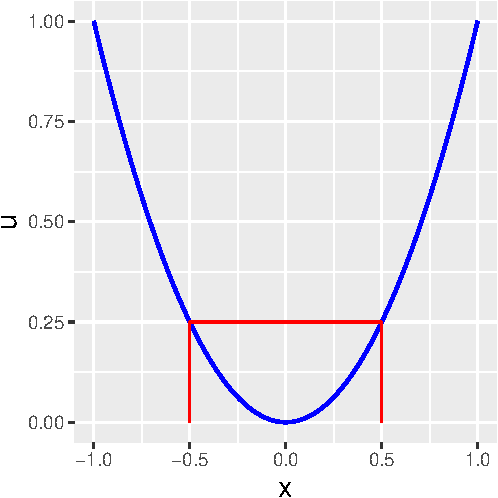
\includegraphics[keepaspectratio]{02-normal_files/figure-latex/fig-noninj-1.pdf}}

}

\caption{\label{fig-noninj}Illustration of the transformation
\(U = X^2\), where the domain of \(f_X(x)\) is \([-1,1]\). The plot
immediately indicates the domain of \(f_U(u)\): {[}0,1{]}. To determine
the functional form of \(f_U(u)\), we note that for any chosen value of
\(u\) (here, 0.25), the range of values of \(X\) that map to
\(U < u = x^2\) are the ones bounded by the two vertical red lines
(here, \(\pm 0.5\)). Hence
\(P(X^2 \leq u) = P(-\sqrt{u} \leq X \leq \sqrt{u})\).}

\end{figure}%

\begin{quote}
Continuing on: \[
F_U(u) = P(-\sqrt{u} \leq X \leq \sqrt{u}) = \int_{-\sqrt{u}}^{\sqrt{u}} \frac12 dx = \left. \frac{x}{2} \right|_{-\sqrt{u}}^{\sqrt{u}} = \sqrt{u} \,,
\] and \[
f_U(u) = \frac{d}{du} \sqrt{u} = \frac{1}{2\sqrt{u}} ~~~ u \in [0,1] \,.
\]
\end{quote}

\subsubsection{Discrete Transformation}\label{discrete-transformation}

\begin{quote}
Let's assume that the probability mass function for a random variable
\(X\) is \[
p_X(x) = p^x (1-p)^{1-x} \,,
\] where \(x \in \{0,1\}\) and \(p \in [0,1]\). Given the transformation
\(U = 2X^2\), what is the pmf for \(U\)?
\end{quote}

\begin{quote}
Because the transformation is injective, the determination of the pmf is
particularly simple and can be done without carrying out the full set of
steps above: we identify that \(X = \sqrt{U/2}\) and state that \[
p_U(u) = p_X\left(\sqrt{\frac{u}{2}}\right) = p^{\sqrt{u/2}} (1-p)^{1-\sqrt{u/2}} \,.
\] Since \(x \in \{0,1\}\), the domain of \(u\) is
\(\{2 \cdot 0^2,2 \cdot 1^2\}\), or \(\{0,2\}\).
\end{quote}

\begin{quote}
Now, what if instead of the pmf above (which is that of the Bernoulli
distribution), we have this pmf instead: \[
p_X(-1) = \frac12 ~~~ \mbox{and} ~~~ p_X(1) = \frac12 \,?
\] This is the pmf for the Rademacher distribution. Because \(U = 2X^2\)
is not an injective function here, we must take care to establish the
mapping of all values in the domain of \(f_X(x)\) to the domain of
\(f_U(u)\): \[
X = -1 ~~~\Rightarrow~~~ U = 2 ~~~~~~\mbox{and}~~~~~~ X = 1 ~~~\Rightarrow~~~ U = 2 \,.
\] Hence \[
p_U(u) = p_X(-1) + p_X(1) = \frac12 + \frac12 = 1 ~~~ u \in \{2\} \,.
\]
\end{quote}

\section{Normal-Related Distribution:
Chi-Square}\label{sec-chap2chisquare}

What to take away from this section:

\begin{itemize}
\item
  If \(Z\) is a standard-normally distributed random variable, \(Z^2\)
  is distributed according to a \emph{chi-square distribution}.
\item
  Via the method of moment-generating functions, we determine that the
  sum of chi-square-distributed random variables is itself a
  chi-square-distributed random variable.
\end{itemize}

The square of a standard normal random variable, \(Z^2\), is an
important quantity that arises, e.g., in statistical model assessment
(through the ``sum of squared errors'' when the ``error'' is normally
distributed) and in hypothesis tests like the chi-square goodness-of-fit
test. But for this quantity to be useful in statistical inference, we
need to know its distribution.

In step (1) of the algorithm laid out in the last section, we identify
the inverse function: if \(U = Z^2\), with \(Z \in (-\infty,\infty)\),
then \(Z = \pm \sqrt{U}\). Then, following step (2), we state that \[
F_U(u) = P(U \leq u) = P(Z^2 \leq u) = P(-\sqrt{u} \leq Z \leq \sqrt{u}) = \Phi(\sqrt{u}) - \Phi(-\sqrt{u}) \,,
\] where, as we recall, \(\Phi(\cdot)\) is the notation for the standard
normal cdf. Because of symmetry, we can simplify this expression: \[
F_U(u) = \Phi(\sqrt{u}) - [1 - \Phi(\sqrt{u})] = 2\Phi(\sqrt{u}) - 1 \,.
\]

To carry out step (3), we utilize the chain rule of differentiation to
determine that the pdf is \begin{align*}
f_U(u) = \frac{d}{du} F_U(u) = \frac{d}{du} [2\Phi(\sqrt{u}) - 1] &= 2 \frac{d\Phi}{du}(\sqrt{u}) \cdot \frac{d}{du}\sqrt{u} \\
&= 2 f_Z(\sqrt{u}) \cdot \frac{1}{2\sqrt{u}} \\
&= \frac{1}{\sqrt{2\pi}} \exp\left(-\frac{u}{2}\right) \cdot \frac{1}{\sqrt{u}} \\
&= \frac{u^{-1/2}}{\sqrt{2\pi}} \exp(-\frac{u}{2}) \,,
\end{align*} with \(u \in [0,\infty)\).

Before continuing, we need to introduce a new probability distribution,
the so-called \emph{chi-square} distribution, which has the probability
density function \[
f_W(x) = \frac{x^{\nu/2-1}}{2^{\nu/2} \Gamma(\nu/2)} \exp\left(-\frac{x}{2}\right) \,,
\] where \(x \geq 0\) and \(\nu\) is a positive integer; \(E[X] = \nu\)
and \(V[X] = 2\nu\). \textbf{Note that we will use the notation \(W\) to
denote a chi-square random variable throughout the remainder of this
book.} The one parameter that dictates the shape of a chi-square
distribution is dubbed the number of \emph{degrees of freedom}, is
conventionally denoted with the Greek letter \(\nu\) (nu, pronounced
``noo''), and has a positive integer value. A chi-square distribution is
highly skew if \(\nu\) is small, but chi-square random variables
converge in distribution to normal random variables as
\(\nu \rightarrow \infty\). See Figure~\ref{fig-chi2}. (As we will see
in Section~\ref{sec-chap4gamma}, the chi-square family of distributions
belongs to the more general gamma family of distributions.)

\begin{figure}

\begin{minipage}[t]{0.50\linewidth}

\centering{

\pandocbounded{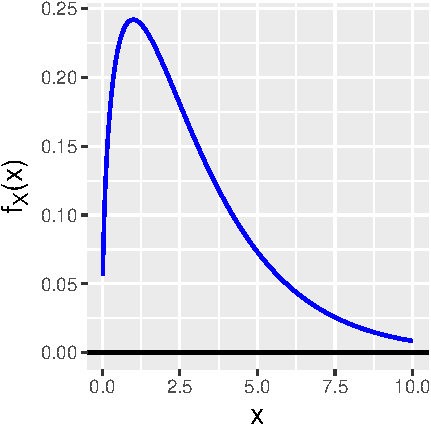
\includegraphics[keepaspectratio]{02-normal_files/figure-latex/fig-chi2-1.pdf}}

}

\subcaption{\label{fig-chi2-1}}

\end{minipage}%
%
\begin{minipage}[t]{0.50\linewidth}

\centering{

\pandocbounded{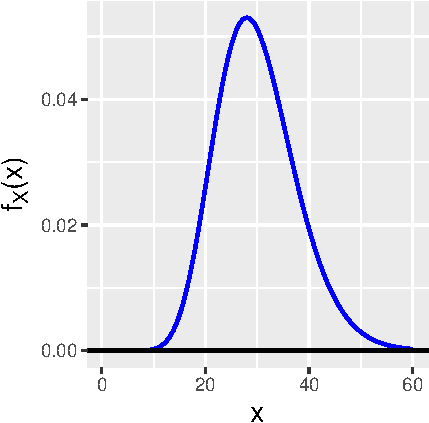
\includegraphics[keepaspectratio]{02-normal_files/figure-latex/fig-chi2-2.pdf}}

}

\subcaption{\label{fig-chi2-2}}

\end{minipage}%

\caption{\label{fig-chi2}Chi-square distributions for (a) \(\nu = 3\)
and (b) \(\nu = 30\) degrees of freedom. Chi-square random variables
converge in distribution to normal random variables as
\(\nu \rightarrow \infty\).}

\end{figure}%

Now let's go back to the result of our transformation. We can now see
that \(f_U(u)\) is a chi-square pdf: \[
U = W \sim \chi_1^2 \,,
\] with the subscript ``1'' indicating that here, \(\nu = 1\).

So: if we take a single standard normal random variable \(Z\) and square
it, the squared value is sampled according to a chi-square distribution
for one degree of freedom. What if now we were to generate a sample of
\(n\) independent standard-normal random variables
\(\{Z_1,\ldots,Z_n\}\)\ldots what is the distribution of
\(\sum_{i=1}^n Z_i^2\)? As this is a sum of independent random
variables, we utilize the method of moment-generating functions to
answer this question. As shown in the first example below, the mgf for a
chi-square random variable is \[
m_W(t) = (1-2t)^{-\nu/2} \,.
\] The mgf of a sum of chi-square random variables, each of which has
\(\nu = 1\) degrees of freedom, will be \[
\prod_{i=1}^n m_{W}(t) = \prod_{i=1}^n (1-2t)^{-\frac{1}{2}} = (1-2t)^{-\frac{n}{2}} \,.
\] We identify the product as being the mgf for a chi-square
distribution with \(\nu = n\) degrees of freedom. Thus: \emph{if we sum
chi-square-distributed random variables, the summed quantity is itself
chi-square distributed, with \(\nu\) being the sum of the numbers of
degrees of freedom for the original random variables.} (This result can
be generalized: for instance, if \(X_1 \sim \chi_a^2\) and
\(X_2 \sim \chi_b^2\), then \(X_1 + X_2 = W \sim \chi_{a+b}^2\).)

\subsection{Examples}\label{examples-18}

\subsubsection{Chi-Square Distribution: Moment-Generating
Function}\label{chi-square-distribution-moment-generating-function}

\begin{quote}
The moment-generating function for a chi-square random variable is \[
E[e^{tX}] = \int_0^\infty e^{tx} \frac{x^{\nu/2-1}}{2^{\nu/2} \Gamma(\nu/2)} e^{-x/2} dx = \int_0^\infty \frac{x^{\nu/2-1}}{2^{\nu/2} \Gamma(\nu/2)} e^{-(1/2-t)x} dx \,.
\] Because the integral bounds are \(0\) and \(\infty\), we utilize a
variable transformation that yields an integrand containing \(e^{-u}\);
we can then evaluate the integral as a gamma function. Thus
\(u = (1/2-t)x\) and \(du = (1/2-t)dx\), with the integral bounds being
unchanged, and we have that \begin{align*}
E[e^{tX}] &= \int_0^\infty \frac{[u/(1/2-t)]^{\nu/2-1}}{2^{\nu/2} \Gamma(\nu/2)} e^{-u} \frac{du}{1/2-t} \\
&= \frac{1}{(1/2-t)^{\nu/2}} \frac{1}{2^{\nu/2}} \frac{1}{\Gamma(\nu/2)} \int_0^\infty u^{\nu/2-1} e^{-u} du \\
&= \frac{1}{(1-2t)^{\nu/2}} \frac{1}{\Gamma(\nu/2)} \Gamma(\nu/2) = (1-2t)^{-\nu/2} \,.
\end{align*}
\end{quote}

\subsubsection{Chi-Square Distribution: Expected
Value}\label{chi-square-distribution-expected-value}

\begin{quote}
The expected value of a chi-square distribution for one degree of
freedom is \begin{align*}
E[X] &= \int_0^\infty x f_X(x) dx \\
&= \int_0^\infty \frac{x^{1/2}}{\sqrt{2\pi}}\exp\left(-\frac{x}{2}\right) dx \,.
\end{align*} To find the value of this integral, we are going to utilize
the gamma function \[
\Gamma(t) = \int_0^\infty u^{t-1} \exp(-u) du \,,
\] which we first introduced in an example in
Section~\ref{sec-chap1lotp}. (Note that \(t > 0\).) Recall that if \(t\)
is an integer, then
\(\Gamma(t) = (t-1)! = (t-1) \times (t-2) \times \cdots \times 1\), with
the exclamation point representing the factorial function. If \(t\) is a
half-integer and small, one can look up the value of \(\Gamma(t)\)
online.
\end{quote}

\begin{quote}
The integral we are trying to compute doesn't quite match the form of
the gamma function integral\ldots but as one should recognize by now, we
can attempt a variable substitution to change \(e^{-x/2}\) to
\(e^{-u}\): \[
u = x/2 ~,~ du = dx/2 ~,~ x = 0 \implies u = 0 ~,~ x = \infty \implies u = \infty
\] We thus rewrite our expected value as \begin{align*}
E[X] &= \int_0^\infty \frac{\sqrt{2}u^{1/2}}{\sqrt{2\pi}} \exp(-u) (2 du) = \frac{2}{\sqrt{\pi}} \int_0^\infty u^{1/2} \exp(-u) du \\
&= \frac{2}{\sqrt{\pi}} \Gamma\left(\frac{3}{2}\right) = \frac{2}{\sqrt{\pi}} \frac{\sqrt{\pi}}{2} = 1 \,.
\end{align*} As we saw above, the sum of \(n\) chi-square random
variables, each distributed with 1 degree of freedom, is itself
chi-square-distributed for \(n\) degrees of freedom. Hence, in general,
if \(W \sim \chi_{n}^2\), then \(E[W] = n\).
\end{quote}

\subsubsection{Computing Probabilities}\label{computing-probabilities-5}

\begin{quote}
Let's assume at first that we have a single random variable
\(Z \sim \mathcal{N}(0,1)\).
\end{quote}

\begin{quote}
\begin{enumerate}
\def\labelenumi{\arabic{enumi}.}
\tightlist
\item
  What is \(P(Z^2 > 1)\)?
\end{enumerate}
\end{quote}

\begin{quote}
We know that \(Z^2\) is sampled according to a chi-square distribution
for 1 degree of freedom. So \[
P(Z^2 > 1) = 1 - P(Z^2 \leq 1) = 1 - F_{W(1)}(1) \,.
\] This is not easily computed by hand, so we utilize \texttt{R}:
\end{quote}

\begin{Shaded}
\begin{Highlighting}[]
\DecValTok{1} \SpecialCharTok{{-}} \FunctionTok{pchisq}\NormalTok{(}\DecValTok{1}\NormalTok{, }\DecValTok{1}\NormalTok{)}
\end{Highlighting}
\end{Shaded}

\begin{verbatim}
[1] 0.3173105
\end{verbatim}

\begin{quote}
The probability is 0.3173. With the benefit of hindsight, we can see why
this was going to be the value all along: we know that
\(P(-1 \leq Z \leq 1) = 0.6827\), and thus
\(P(\vert Z \vert > 1) = 1-0.6827 = 0.3173\). If we square both sides in
this last probability statement, we see that \(P(\vert Z \vert > 1) =
P(Z^2 > 1)\).
\end{quote}

\begin{quote}
\begin{enumerate}
\def\labelenumi{\arabic{enumi}.}
\setcounter{enumi}{1}
\tightlist
\item
  What is the value \(a\) such that \(P(W > a) = 0.9\), where
  \(W = Z_1^2 + \cdots + Z_4^2\) and \(\{Z_1,\ldots,Z_4\}\) are iid
  standard normal random variables?
\end{enumerate}
\end{quote}

\begin{quote}
First, we recognize that \(W \sim \chi_4^2\), i.e., \(W\) is chi-square
distributed for 4 degrees of freedom.
\end{quote}

\begin{quote}
Second, we re-express \(P(W > a)\) in terms of the cdf of the chi-square
distribution, \[
P(W > a) = 1 - P(W \leq a) = 1 - F_{W(4)}(a) = 0.9 \,,
\] and we rearrange terms: \[
F_{W(4)}(a) = 0.1 \,.
\] To isolate \(a\), we use the inverse CDF function: \[
F_{W(4)}^{-1} [F_{W(4)}(a)] = a = F_{W(4)}^{-1}(0.1) \,.
\] To compute \(a\), we use the \texttt{R} function \texttt{qchisq()}:
\end{quote}

\begin{Shaded}
\begin{Highlighting}[]
\NormalTok{(}\AttributeTok{a =} \FunctionTok{qchisq}\NormalTok{(}\FloatTok{0.1}\NormalTok{, }\DecValTok{4}\NormalTok{))}
\end{Highlighting}
\end{Shaded}

\begin{verbatim}
[1] 1.063623
\end{verbatim}

\begin{quote}
We find that \(a = 1.064\).
\end{quote}

\section{Normal Distribution: Sample Variance}\label{sec-chap2variance}

What to take away from this section:

\begin{itemize}
\item
  The quantity \(W = (n-1)S^2/\sigma^2\) is a
  \emph{chi-square-distributed random variable}.
\item
  Combining this result with the transformation
  \(S^2 = \sigma^2 W / (n-1)\), we determine that the normal sample
  variance \(S^2\) is distributed according to a \emph{gamma
  distribution}.
\item
  Foreshadowing: this result will allow us to make statistical
  inferences about the normal population variance \(\sigma^2\) given
  \(n\) iid normal random variables.
\end{itemize}

Recall the definition of the sample variance: \[
S^2 = \frac{1}{n-1} \sum_{i=1}^n (X_i - \bar{X})^2 = \frac{1}{n-1} \left[ \left( \sum_{i=1}^n X_i^2 \right) - n\bar{X}^2 \right] \,.
\] The reason why we divide by \(n-1\) instead of \(n\) is that it makes
\(S^2\) an unbiased estimator of \(\sigma^2\). We will illustrate this
point below when we cover point estimation.

Previously, we showed how the sample mean of iid normal random variables
is itself normal, with mean \(\mu\) and variance \(\sigma^2/n\). What,
on the other hand, is the distribution of \(S^2\)?

We could try to derive this directly, by utilizing transformations and
the method of moment-generating functions, but we would run into the
issue that, e.g., \(\sum_{i=1}^n X_i^2\) and \(\bar{X}^2\) are not
independent random variables. So we will attack this derivation a bit
more indirectly instead.

Suppose that we have \(n\) iid normal random variables. We can write
down that \[
\sum_{i=1}^n \left( \frac{X_i-\mu}{\sigma} \right)^2 = W \sim \chi_n^2 \,.
\] We can work with the expression to the left of the equals sign to
determine the distribution of \((n-1)S^2/\sigma^2\): \begin{align*}
\sum_{i=1}^n \left( \frac{X_i-\mu}{\sigma} \right)^2 &= \sum_{i=1}^n \left( \frac{(X_i-\bar{X})+(\bar{X}-\mu)}{\sigma} \right)^2 \\
&= \sum_{i=1}^n \left( \frac{X_i-\bar{X}}{\sigma}\right)^2 + \sum_{i=1}^n \left( \frac{\bar{X}-\mu}{\sigma}\right)^2 + \mbox{cross~term~equaling~zero} \\
&= \frac{(n-1)S^2}{\sigma^2} + n\left(\frac{\bar{X}-\mu}{\sigma}\right)^2 = \frac{(n-1)S^2}{\sigma^2} + \left(\frac{\bar{X}-\mu}{\sigma/\sqrt{n}}\right)^2 \,.
\end{align*} The expression farthest to the right contains the quantity
\[
\frac{\bar{X}-\mu}{\sigma/\sqrt{n}} \,,
\] which, since \(\bar{X} \sim \mathcal{N}(\mu,\sigma^2/n)\), is a
standard normal random variable. Thus the expression itself represents a
chi-square-distributed random variable for 1 dof. Recall that if
\(X_1 \sim \chi_a^2\) and \(X_2 \sim \chi_b^2\), then \(X_1 + X_2 \sim
\chi_{a+b}^2\); given this, it must be the case that \[
\frac{(n-1)S^2}{\sigma^2} = W' \sim \chi_{n-1}^2 \,.
\]

\emph{Now} we can determine the distribution of \(S^2\), by utilizing
the transformation \[
S^2 = \frac{\sigma^2 W'}{n-1} \,.
\] We have that \begin{align*}
F_{S^2}(x) &= P(S^2 \leq x) = P\left( \frac{\sigma^2 W'}{n-1} \leq x \right)\\
&= P\left( W' \leq \frac{(n-1)x}{\sigma^2} \right) = F_{W'}\left(\frac{(n-1)x}{\sigma^2} \right) \,,
\end{align*} and thus \begin{align*}
f_{S^2}(x) &= \frac{d}{dx} F_{S^2}(x) = f_{S^2}\left(\frac{(n-1)x}{\sigma^2} \right) \frac{(n-1)}{\sigma^2} \\
&= \frac{\left[\frac{(n-1)x}{\sigma^2}\right]^{(n-1)/2 - 1}}{2^{(n-1)/2} \Gamma\left((n-1)/2\right)} \exp\left(-\frac{(n-1)x}{2\sigma^2}\right) \frac{(n-1)}{\sigma^2} \,.
\end{align*} If we let \(a = (n-1)/2\) and \(b = 2\sigma^2/(n-1)\), then
the pdf above becomes \[
f_{S^2}(x) = \frac{x^{a-1}}{b^a\Gamma(a)} \exp\left(-\frac{x}{b}\right) \,.
\] This is the pdf of a \emph{gamma distribution} with shape parameter
\(a\) and scale parameter \(b\), i.e., \[
S^2 \sim \mbox{Gamma}\left(\frac{n-1}{2},\frac{2\sigma^2}{n-1}\right) \,.
\] We will officially introduce the gamma distribution in
Section~\ref{sec-chap4gamma}; for now, it suffices to say that if \(X\)
is a gamma-distributed random variable, then \(E[X] = ab\) and
\(V[X] = ab^2\)\ldots thus \(E[S^2] = \sigma^2\) and
\(V[S^2] = 2\sigma^4/(n-1)\).

\subsection{Examples}\label{examples-19}

\subsubsection{Computing Probabilities}\label{computing-probabilities-6}

\begin{quote}
Let's suppose we sample \(16\) iid normal random variables, and we know
that \(\sigma^2 = 10\). What is the probability \(P(S^2 > 12)\)?
\end{quote}

\begin{quote}
(We'll stop for a moment to answer a question that might occur to the
reader. ``Why are we doing a problem where we assume \(\sigma^2\) is
known? In real life, it almost certainly won't be.'' This is an entirely
fair question. This example \emph{is} contrived, but it builds towards a
particular situation where we \emph{can} assume a value for
\(\sigma^2\): hypothesis testing. The calculation we do below is
analogous to calculations we will do later when testing hypotheses about
normal population variances.)
\end{quote}

\begin{quote}
To compute the probability, we write
\(P(S^2 > 12) = 1 - P(S^2 \leq 12)\) and utilize the cdf of a gamma
distribution:
\end{quote}

\begin{Shaded}
\begin{Highlighting}[]
\NormalTok{n      }\OtherTok{\textless{}{-}} \DecValTok{16}
\NormalTok{sigma2 }\OtherTok{\textless{}{-}} \DecValTok{10}
\NormalTok{a      }\OtherTok{\textless{}{-}}\NormalTok{ (n }\SpecialCharTok{{-}} \DecValTok{1}\NormalTok{) }\SpecialCharTok{/} \DecValTok{2}
\NormalTok{b      }\OtherTok{\textless{}{-}} \DecValTok{2} \SpecialCharTok{*}\NormalTok{ sigma2}\SpecialCharTok{/}\NormalTok{ (n }\SpecialCharTok{{-}} \DecValTok{1}\NormalTok{)}
\DecValTok{1} \SpecialCharTok{{-}} \FunctionTok{pgamma}\NormalTok{(}\DecValTok{12}\NormalTok{, }\AttributeTok{shape =}\NormalTok{ a, }\AttributeTok{scale =}\NormalTok{ b)}
\end{Highlighting}
\end{Shaded}

\begin{verbatim}
[1] 0.2626656
\end{verbatim}

\subsubsection{Expected Value of the Standard
Deviation}\label{expected-value-of-the-standard-deviation}

\begin{quote}
Above, we determined that when we sample \(n\) iid data according to a
normal distribution, the sample variance \(S^2\) is gamma-distributed
with shape parameter \(a = (n-1)/2\) and scale parameter
\(b = 2\sigma^2/(n-1)\), and the expected value of \(S^2\) is
\(\sigma^2\)\ldots meaning that \(S^2\) is an unbiased estimator for
population variance \(\sigma^2\).
\end{quote}

\begin{quote}
A natural question which then arises is: is the sample standard
deviation \(S\) an unbiased estimator for the population standard
deviation \(\sigma\)?
\end{quote}

\begin{quote}
To answer this, we first must determine the probability distribution
function \(f_S(x)\). This is straightforwardly done via the
transformation \(S = \sqrt{S^2}\): \[
F_S(x) = P(S \leq x) = P(\sqrt{S^2} \leq x) = P(S^2 \leq x^2) = F_{S^2}(x^2) \,,
\] and thus \[
f_S(x) = \frac{d}{dx} F_S(x) = 2 x f_{S^2}(x^2) = 2 x \frac{(x^2)^{a-1}}{b^a \Gamma(a)} \exp\left(-\frac{x^2}{b}\right) \,,
\] where \(x > 0\). (Note that this distribution has a name: it is a
Nakagami distribution.)
\end{quote}

\begin{quote}
The expected value of \(S\) is \[
E[S] = \int_0^\infty 2 x^2 \frac{(x^2)^{a-1}}{b^a \Gamma(a)} \exp\left(-\frac{x^2}{b}\right) dx = 2 \left(\frac{x^2}{b}\right)^a \frac{1}{\Gamma(a)} \exp\left(-\frac{x^2}{b}\right) dx \,.
\] Given the integral bounds, we utilize the variable transformation
\(t = x^2/b\), such that \(dt = 2 x dx/b\) (with the integral bounds
being unchanged). Thus \begin{align*}
E[S] &= \frac{2}{\Gamma(a)} \int_0^\infty t^a \exp(-t) \frac12 \sqrt{\frac{b}{t}} dt \\
&= \frac{\sqrt{b}}{\Gamma(a)} \int_0^\infty t^{a-1/2} \exp(-t) dt \\
&= \frac{\Gamma(a+1/2)}{\Gamma(a)} \sqrt{b} \\
&= \frac{\Gamma(n/2)}{\Gamma((n-1)/2)} \sqrt{\frac{2}{n-1}} \sigma \neq \sigma \,.
\end{align*} We thus find that \(S\) is a \emph{biased} estimator of the
normal standard deviation \(\sigma\). We note that \[
\lim_{n \to \infty} \frac{\Gamma(n/2)}{\Gamma((n-1)/2)} = \lim_{n \to \infty} \frac{\Gamma((n-1)/2 + 1/2)}{\Gamma((n-1)/2)} = \left(\frac{n-1}{2}\right)^{1/2} \,,
\] so asymptotically \(S\) is an unbiased estimator for \(\sigma\).
\end{quote}

\section{Normal-Related Distribution: t}\label{sec-chap2t}

What to take away from this section:

\begin{itemize}
\item
  The quantity \(t = (\bar{X}-\mu)/(\sigma/\sqrt{n})\) is a
  \emph{t-distributed random variable}.
\item
  Foreshadowing: this result will allow us to make statistical
  inferences about the normal population mean \(\mu\), given \(n\) iid
  normal random variables, even when the population variance
  \(\sigma^2\) is unknown.
\end{itemize}

It is generally the case in real-life that when we assume our data are
sampled according to a normal distribution, both the mean \emph{and} the
variance are unknown. This means that instead of \[
Z = \frac{\bar{X}-\mu}{\sigma/\sqrt{n}} \sim \mathcal{N}(0,1) \,,
\] we have \[
\frac{\bar{X}-\mu}{S/\sqrt{n}} \sim \mbox{?}
\] This last expression contains \emph{two} random variables, one in the
numerator and one in the denominator, and each is independent of the
other. (We state this without proof\ldots but we will appeal to
intuition. For many distributions, the expected value and variance are
\emph{both} functions of one or more parameters \(\theta\) {[}e.g., the
exponential, binomial, and Poisson distributions, etc., etc.{]}.
However, for a normal distribution, the expected value only depends on
\(\mu\) and the variance only depends on \(\sigma^2\).) How would we
determine the distribution of the ratio above?

There is no unique way by which to approach the derivation of the
distribution: we simply illustrate one way of doing so. First, we
rewrite the ratio above as \begin{align*}
T = \frac{\bar{X}-\mu}{S/\sqrt{n}} &= \frac{\bar{X}-\mu}{\sigma/\sqrt{n}} / \frac{S}{\sigma} = \frac{\bar{X}-\mu}{\sigma/\sqrt{n}} / \sqrt{\frac{S^2}{\sigma^2}}\\
&= \frac{\bar{X}-\mu}{\sigma/\sqrt{n}} / \left( \sqrt{\frac{\nu S^2}{\sigma^2}} \frac{1}{\sqrt{\nu}} \right) = Z / \left(\sqrt{\frac{W}{\nu}}\right) \,,
\end{align*} where \(Z \sim \mathcal{N}(0,1)\) and \(W\) is sampled
according to a chi-square distribution with \(\nu = n-1\) degrees of
freedom. Our next step is to determine the distribution of the random
variable \(U = \sqrt{W/\nu}\). We identify that \(V = \sqrt{W}\) is
sampled according to a \emph{chi distribution} (note: no square!), whose
pdf may be derived via a general transformation (since
\(V = \sqrt{\nu}S/\sigma\) and since we have written down \(f_S(x)\)
above), but can also simply be looked up: \[
f_V(x) = \frac{x^{\nu-1} \exp(-x^2/2)}{2^{\nu/2-1}\Gamma(\nu/2)} \,,
\] for \(x \geq 0\) and \(\nu > 0\). However, we \emph{do} still have to
apply a general transformation to determine the pdf for
\(U = V/\sqrt{\nu}\). Doing so, we find that \[
f_U(x) = f_V(\sqrt{\nu}x) \sqrt{\nu} = \frac{\sqrt{\nu} (\sqrt{\nu}x)^{\nu-1} \exp(-(\sqrt{\nu}x)^2/2)}{2^{\nu/2-1}\Gamma(\nu/2)} \,.
\] (So, yes, we could have derived \(f_U(x)\) directly from \(f_S(x)\)
via a general transformation\ldots but here we at least indicate to the
reader that there is such a thing as the chi distribution.)

At this point, we know the distributions for both the numerator and the
denominator. Now we write down a general result dubbed the \emph{ratio
distribution}. For \(T = Z/U\), where \(Z\) and \(U\) are independent
variables, that distribution is \[
f_T(t) = \int_{-\infty}^\infty \vert u \vert f_Z(tu) f_{U}(u) du \rightarrow \int_0^\infty u f_Z(tu) f_{U}(u) du \,,
\] where we make use of the fact that \(u > 0\). Thus \begin{align*}
f_T(t) &= \int_0^\infty u \frac{1}{\sqrt{2\pi}} \exp\left(-\frac{t^2u^2}{2}\right) \frac{\sqrt{\nu} (\sqrt{\nu}u)^{\nu-1} \exp(-(\sqrt{\nu}u)^2/2)}{2^{\nu/2-1}\Gamma(\nu/2)} du \\
&= \frac{1}{\sqrt{2\pi}} \frac{1}{2^{\nu/2-1}\Gamma(\nu/2)} \nu^{\nu/2} \int_0^\infty u^\nu \exp\left(-\frac{(t^2+\nu)u^2}{2}\right) du \,.
\end{align*} Given the form of the integral and the fact that it is
evaluated from zero to infinity, we will use a variable substitution
approach and eventually turn the integral into a gamma function: \[
x = \frac{(t^2+\nu)u^2}{2} ~~~ \Rightarrow ~~~ dx = (t^2+\nu)~u~du \,.
\] When \(u = 0\), \(x = 0\), and when \(u = \infty\), \(x = \infty\),
so the integral bounds are unchanged. Hence we can rewrite the integral
above as \begin{align*}
f_T(t) &= \frac{1}{\sqrt{2\pi}} \frac{1}{2^{\nu/2-1}\Gamma(\nu/2)} \nu^{\nu/2} \int_0^\infty \left(\sqrt{\frac{2x}{(t^2+\nu)}}\right)^\nu \exp\left(-x\right) \frac{dx}{\sqrt{2 x (t^2+\nu)}} \\
&= \frac{1}{\sqrt{2\pi}} \frac{1}{2^{\nu/2-1}\Gamma(\nu/2)} \nu^{\nu/2} 2^{\nu/2} 2^{-1/2} \frac{1}{(t^2+\nu)^{(\nu+1)/2}} \int_0^\infty \frac{x^{\nu/2}}{x^{1/2}} \exp\left(-x\right) dx \\
&= \frac{1}{\sqrt{\pi}} \frac{1}{\Gamma(\nu/2)} \nu^{\nu/2} \frac{1}{(t^2+\nu)^{(\nu+1)/2}} \int_0^\infty x^{\nu/2-1/2} \exp\left(-x\right) dx \\
&= \frac{1}{\sqrt{\pi}} \frac{1}{\Gamma(\nu/2)} \nu^{\nu/2} \frac{1}{(t^2+\nu)^{(\nu+1)/2}} \Gamma((\nu+1)/2) \\
&= \frac{1}{\sqrt{\pi}} \frac{\Gamma((\nu+1)/2)}{\Gamma(\nu/2)} \nu^{\nu/2} \frac{1}{\nu^{(\nu+1)/2}(t^2/\nu+1)^{(\nu+1)/2}} \\
&= \frac{1}{\sqrt{\nu \pi}} \frac{\Gamma((\nu+1)/2)}{\Gamma(\nu/2)} \left(1+\frac{t^2}{\nu}\right)^{-(\nu+1)/2} \,.
\end{align*} \(T\) is sampled according to a \emph{Student's t
distribution} for \(\nu\) degrees of freedom. Assuming that \(\nu\) is
integer-valued, the expected value of \(T\) is \(E[T] = 0\) for
\(\nu \geq 2\) (and is undefined otherwise), while the variance is
\(\nu/(\nu-2)\) for \(\nu \geq 3\), is infinite for \(\nu=2\), and is
otherwise undefined. Appealing to intuition, we can form a (symmetric)
\(t\) distribution by taking a standard normal \(\mathcal{N}(0,1)\) and
``pushing down'' in the center, the act of which transfers probability
density equally to both the lower and upper tails. In
Figure~\ref{fig-t}, we see that the smaller the number of degrees of
freedom, the more density is transferred to the tails, and that as
\(\nu\) increases, the more and more \(f_{T(\nu)}(t)\) becomes
indistinguishable from a standard normal. (The more technical way of
stating this is that the random variable \(T\) converges in distribution
to a standard normal random variable as \(\nu \rightarrow \infty\).)

\begin{figure}

\centering{

\pandocbounded{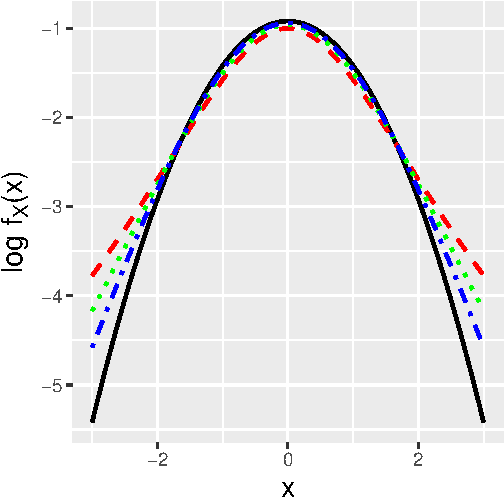
\includegraphics[keepaspectratio]{02-normal_files/figure-latex/fig-t-1.pdf}}

}

\caption{\label{fig-t}The natural logarithm of the pdf for the standard
normal (black) and for \(t\) distributions with 3 (red dashed), 6 (green
dotted), and 12 (blue dot-dashed) degrees of freedom. We observe that as
\(n\) decreases, there is more probability density in the lower and
upper tails of the distributions.}

\end{figure}%

\subsection{Example}\label{example-3}

\subsubsection{Computing Probabilities}\label{computing-probabilities-7}

\begin{quote}
In a study, the diameters of \(n = 8\) widgets are measured. It is known
from previous work that the widget diamaters are normally distributed,
with sample standard deviation \(S = 1\) unit. What is the probability
that the the sample mean \(\bar{X}\) observed in the current study will
be within one unit of the population mean \(\mu\)?
\end{quote}

\begin{quote}
The probability we seek is \[
P( \vert \bar{X} - \mu \vert < 1 ) = P(\mu - 1 \leq \bar{X} \leq \mu + 1) \,.
\] The key here is that we don't know \(\sigma\), so the probability can
only be determined if we manipulate this expression such that the random
variable inside it is \(t\)-distributed\ldots and \(\bar{X}\) itself is
\emph{not}. So the first step is to standardize: \[
P\left( \frac{\mu - 1 - \mu}{S/\sqrt{n}} \leq \frac{\bar{X} - \mu}{S/\sqrt{n}} \leq \frac{\mu + 1 - \mu}{S/\sqrt{n}}\right) = P\left( -\frac{\sqrt{n}}{S} \leq T \leq \frac{\sqrt{n}}{S}\right) \,.
\] We know that \(\sqrt{n}(\bar{X} - \mu)/S\) is \(t\)-distributed (with
\(\nu = n-1\) degrees of freedom), so long as the individual data are
normal iid random variables. (If the individual data are not normally
distributed, this question might have to be solved via
simulations\ldots if we cannot determine the distribution of \(\bar{X}\)
using, e.g., moment-generating functions.)
\end{quote}

\begin{quote}
The probability is the difference between two cdf values: \[
P\left( -\frac{\sqrt{n}}{S} \leq T \leq \frac{\sqrt{n}}{S}\right) = F_{T(7)}(\sqrt{8}) - F_{T(7)}(-\sqrt{8}) \,,
\] where \(n-1\), the number of degrees of freedom, is 7. This is the
end of the problem if we are using pen and paper. If we have \texttt{R}
at our disposal, we would code the following:
\end{quote}

\begin{Shaded}
\begin{Highlighting}[]
\FunctionTok{round}\NormalTok{(}\FunctionTok{pt}\NormalTok{(}\FunctionTok{sqrt}\NormalTok{(}\DecValTok{8}\NormalTok{), }\DecValTok{7}\NormalTok{) }\SpecialCharTok{{-}} \FunctionTok{pt}\NormalTok{(}\SpecialCharTok{{-}}\FunctionTok{sqrt}\NormalTok{(}\DecValTok{8}\NormalTok{), }\DecValTok{7}\NormalTok{), }\DecValTok{3}\NormalTok{)}
\end{Highlighting}
\end{Shaded}

\begin{verbatim}
[1] 0.975
\end{verbatim}

\begin{quote}
The probability that \(\bar{X}\) will be within one unit of \(\mu\) is
0.975.
\end{quote}

\section{Point Estimation}\label{sec-chap2point}

What to take away from this section:

\begin{itemize}
\item
  As discussed in Section~\ref{sec-chap1point}, we can determine the
  quality of proposed point estimators using the metrics of bias,
  variance, and mean-squared error.
\item
  A \emph{consistent estimator} is one whose mean-squared error goes to
  zero as the sample size \(n\) goes to infinity.
\item
  Under certain regularity conditions, we can determine the minimum
  variance of an unbiased point estimator of \(\theta\) by first
  computing its \emph{Fisher information} content, and then using that
  result to derive the \emph{Cramer-Rao lower bound} on the variance.
\item
  Asymptotically, a maximum likelihood estimator for \(\theta\)
  converges in distribution to a normal random variable with mean
  \(\theta\) and variance given by the CRLB.
\end{itemize}

For previous material on point estimation, see
Section~\ref{sec-chap1point}.

In Section~\ref{sec-chap1point}, we introduced the concept of point
estimation, using statistics to make inferences about a population
parameter \(\theta\). Recall that a point estimator \(\hat{\theta}\),
being a statistic, is a random variable and has a sampling distribution.
One can define point estimators arbitrarily, but in the end, we can
choose the best among a set of estimators by assessing properties of
their sampling distributions:

\begin{itemize}
\tightlist
\item
  Bias: \(B[\hat{\theta}] = E[\hat{\theta}-\theta]\)
\item
  Variance: \(V[\hat{\theta}]\)
\end{itemize}

\smallskip\hrule

\begin{quote}
\textbf{Recall}: \emph{the bias of an estimator is the difference
between the average value of the estimates it generates and the true
parameter value. If \(E[\hat{\theta}-\theta] = 0\), then the estimator
\(\hat{\theta}\) is said to be unbiased.}
\end{quote}

\smallskip\hrule

Assuming that our observed data are independent and identically
distributed (or iid), then computing each of these quantities is
straightforward. Choosing a best estimator based on these two quantities
might not lead to a clear answer, but we can overcome that obstacle by
combining them into one metric, the mean-squared error (or MSE):

\begin{itemize}
\tightlist
\item
  MSE: \(MSE[\hat{\theta}] = B[\hat{\theta}]^2 + V[\hat{\theta}]\)
\end{itemize}

In Section~\ref{sec-chap1point}, we also discussed how guessing the form
of an estimator is sub-optimal, and how there are various approaches to
deriving good estimators. The first one that we highlight is maximum
likelihood estimation (or MLE). We will apply the MLE here to derive an
estimator for the normal population mean. Then we will introduce
methodology by which to assess the estimator in an absolute sense, and
extend these results to write down the asymptotic sampling distribution
for the MLE, i.e., the sampling distribution as the sample size
\(n \rightarrow \infty\).

\smallskip\hrule

\begin{quote}
\textbf{Recall}: \emph{the value of \(\theta\) that maximizes the
likelihood function is the maximum likelihood estimate, or MLE, for
\(\theta\). The maximum is found by taking the (partial) derivative of
the (log-)likelihood function with respect to \(\theta\), setting the
result to zero, and solving for \(\theta\). That solution is the maximum
likelihood estimate \(\hat{\theta}_{MLE}\). Also recall the invariance
property of the MLE: if \(\hat{\theta}_{MLE}\) is the MLE for
\(\theta\), then \(g(\hat{\theta}_{MLE})\) is the MLE for
\(g(\theta)\).}
\end{quote}

\smallskip\hrule

The setting, again, is that we have randomly sampled \(n\) data from a
normal distribution with parameters \(\mu\) and \(\sigma\). This means
that the likelihood function is \begin{align*}
\mathcal{L}(\mu,\sigma \vert \mathbf{x}) &= \prod_{i=1}^n f_X(x \vert \mu,\sigma) \\ 
&= \prod_{i=1}^n \frac{1}{\sqrt{2 \pi \sigma^2}} \exp\left(-\frac{(x_i-\mu)^2}{2\sigma^2}\right) \\
&= \frac{1}{(2 \pi)^{n/2}} \frac{1}{\sigma^n} \exp\left({-\frac{1}{2\sigma^2}\sum_{i=1}^n (x_i - \mu)^2}\right) \,,
\end{align*} and the log-likelihood is \[
\ell(\mu,\sigma \vert \mathbf{x}) = -\frac{n}{2} \log (2 \pi) - n \log \sigma - \frac{1}{\sigma^2} \sum_{i=1}^n (x_i - \mu)^2 \,.
\] Because there is more than one parameter, we take the partial
derivative of \(\ell\) with respect to \(\mu\): \begin{align*}
\ell'(\mu,\sigma \vert \mathbf{x}) &= \frac{\partial}{\partial \mu} \left( -\frac{n}{2} \log (2 \pi) - n \log \sigma - \frac{1}{\sigma^2} \sum_{i=1}^n (x_i - \mu)^2 \right) \\
&= -\frac{1}{\sigma^2} \sum_{i=1}^n 2(x_i - \mu)(-1) \\
&= \frac{2}{\sigma^2} \sum_{i=1}^n (x_i - \mu) \,.
\end{align*} After setting this quantity to zero and dividing out the
term \(2/\sigma^2\), we find that \[
\sum_{i=1}^n x_i = \sum_{i=1}^n \mu ~~\Rightarrow~~ \sum_{i=1}^n x_i = n \mu ~~\Rightarrow~~ \frac{1}{n} \sum_{i=1}^n x_i = n \mu ~~\Rightarrow~~ \mu = \bar{x} \,,
\] and thus \(\hat{\mu}_{MLE} = \bar{X}\). (Recall that as we go from a
purely mathematical derivation to a final definition of an estimator, we
need to take into account that the estimator is a random variable and
thus we need to change from lower-case to upper-case when writing out
the variable. Also recall that for this MLE to be valid, the second
derivative of the log-likelihood function
\(\ell(\theta \vert \mathbf{x})\) at \(x = \bar{x}\) has to be negative.
We leave checking this as an exercise to the reader.)

Because the estimator is \(\bar{X}\), we know immediately its expected
value and variance given previous results:

\begin{itemize}
\tightlist
\item
  \(E[\hat{\mu}_{MLE}] = E[\bar{X}] = \mu\) (the estimator is unbiased);
  and
\item
  \(V[\hat{\mu}_{MLE}] = V[\bar{X}] = \sigma^2/n\) (and thus
  \(MSE[\hat{\mu}_{MLE}] = \sigma^2/n\)).
\end{itemize}

While \(\hat{\mu}_{MLE}\) is an unbiased estimator, recall that MLEs can
be biased\ldots but if they are, they are always asymptotically
unbiased, meaning that the bias goes away as \(n \rightarrow \infty\).

\subsection{Point Estimation: Consistency}\label{sec-chap2consistency}

Here, we will introduce one more estimator concept, that of
\emph{consistency}: do both the bias and the variance of the estimator
go to zero as the sample size \(n\) increases? If so, our estimator is
said to be consistent. If an estimator is not consistent, it will never
converge to the true value \(\theta\), regardless of sample size. Here,
we need not worry about the bias (\(\hat{\mu}_{MLE} = \bar{X}\) in
unbiased for all \(n\)), and we note that \[
\lim_{n \rightarrow \infty} \frac{\sigma^2}{n} = 0 \,.
\] Thus \(\hat{\mu}_{MLE}\) is a consistent estimator.

\subsection{Point Estimation: Cramer-Rao Lower Bound and Fisher
Information}\label{sec-chap2crlb}

The question that we are going to pose now refers to a point made
obliquely in Section~\ref{sec-chap1point}: how do we assess
\(V[\hat{\mu}_{MLE}]\) in absolute terms? Can we come up with an
estimator that is more accurate for any given value of \(n\)?

The answer lies in the \emph{Cramer-Rao inequality}, which specifies the
lower bound on the variance of an estimator (so long as the domain of
\(p_X(x \vert \theta)\) or \(f_X(x \vert \theta)\) does not depend on
\(\theta\) itself\ldots which is true for the normal). In this work, we
focus on determining lower bounds for \emph{unbiased} estimators, but
bounds can be found for biased estimators as well, as shown
\href{https://en.wikipedia.org/wiki/Cram\%C3\%A9r\%E2\%80\%93Rao_bound}{here}.

If we sample \(n\) iid data, then the \emph{Cramer-Rao lower bound}
(CRLB) on the variance of an unbiased estimator \(\hat{\theta}\) is \[
V[\hat{\theta}] = \frac{1}{I_n(\theta)} = \frac{1}{nI(\theta)} \,,
\] where \(I(\theta)\) represents the \emph{Fisher information} for
\(\theta\) contained in a single random variable \(X\). Assuming we
sample our data from a pdf, the Fisher information is \[
I(\theta) = E\left[\left(\frac{\partial}{\partial \theta} \log f_X(x \vert \theta) \right)^2\right] ~~~\mbox{or}~~~ I(\theta) = -E\left[ \frac{\partial^2}{\partial \theta^2} \log f_X(x \vert \theta) \right] \,.
\] (The equation to the right is valid only under certain regularity
conditions, but those conditions are usually met in the context of this
book and thus this is the equation that we will use in general, as it
makes for more straightforward computation.) Let's step back for a
second and think about what the Fisher information represents. It is the
average value of the square of the first derivative of a pdf. If a pdf's
slope is relatively small (because the pdf is wide, like a normal with a
large \(\sigma\) parameter), then the average value of the slope,
squared, is relatively small, i.e., the information that \(X\) provides
about \(\mu\) or \(\sigma\) is relatively small. This makes intuitive
sense: a wide pdf means that, for instance, when we sample data and try
to subsequently estimate \(\theta\), we will be more uncertain about its
actual value. On the other hand, if the pdf is highly concentrated, then
the average slope of the pdf is larger and\ldots{}\(I(\theta)\) is
relatively large; a sampled datum would contain more information by
which to constrain \(\theta\). (See Figure~\ref{fig-fisher}, in which
the pdf to the left has less Fisher information content about \(\mu\)
than the pdf to the right.)

\begin{figure}

\begin{minipage}[t]{0.50\linewidth}

\centering{

\pandocbounded{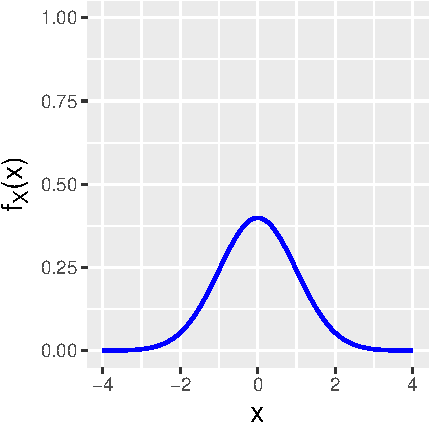
\includegraphics[keepaspectratio]{02-normal_files/figure-latex/fig-fisher-1.pdf}}

}

\subcaption{\label{fig-fisher-1}}

\end{minipage}%
%
\begin{minipage}[t]{0.50\linewidth}

\centering{

\pandocbounded{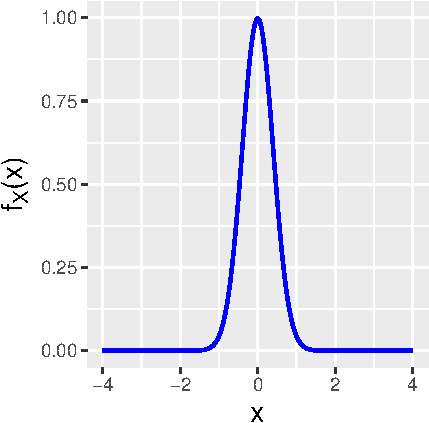
\includegraphics[keepaspectratio]{02-normal_files/figure-latex/fig-fisher-2.pdf}}

}

\subcaption{\label{fig-fisher-2}}

\end{minipage}%

\caption{\label{fig-fisher}An illustration of Fisher information. For
the pdf in (a), the slope changes slowly, and thus the rate of change of
the slope is smaller than for the pdf in (b). Thus the pdf to the left
contains less information about the population mean, i.e., its Fisher
information value \(I(\mu)\) is smaller.}

\end{figure}%

For the normal, \begin{align*}
\log f_X(X \vert \mu) &= -\frac{1}{2} \log (2\pi\sigma^2) - \frac{(x - \mu)^2}{2\sigma^2} \\
\frac{\partial}{\partial \mu} \log f_X(X \vert \mu) &= 0 - \frac{2(x-\mu)(-1)}{2\sigma^2} = \frac{(x-\mu)}{\sigma^2} \\
\frac{\partial^2}{\partial \mu^2} \log f_X(X \vert \mu) &= -\frac{1}{\sigma^2} \,,
\end{align*} so \[
I(\mu) = -E\left[-\frac{1}{\sigma^2}\right] = \frac{1}{\sigma^2} \,,
\] and \[
V[\hat{\mu}] = \frac{1}{n (1/\sigma^2)} = \frac{\sigma^2}{n} \,.
\] We see that the variance of \(\hat{\mu} = \bar{X}\) achieves the
CRLB, meaning that indeed we cannot propose a better unbiased estimator
for the normal population mean.

\subsection{Point Estimation: Asymptotic Distribution of the
MLE}\label{sec-chap2mle}

We conclude this section by using the Fisher information to state an
important result about maximum likelihood estimates. Recall that an
estimator is a statistic, and thus it is a random variable with a
sampling distribution. What do we know about this distribution? For
arbitrary values of \(n\), nothing, per se; we would have to run
simulations to derive an empirical sampling distribution. However, as
\(n \rightarrow \infty\), the MLE converges in distribution to a normal
random variable: \[
\sqrt{n}(\hat{\theta}_{MLE}-\theta) \overset{d}{\rightarrow} Y \sim \mathcal{N}\left(0,\frac{1}{I(\theta)}\right) ~\mbox{or}~ (\hat{\theta}_{MLE}-\theta) \overset{d}{\rightarrow} Y' \sim \mathcal{N}\left(0,\frac{1}{nI(\theta)}\right) \,.
\] (As usual, some regularity conditions apply that do not concern us at
the current time.) We already knew about the mean zero part: we had
stated that the MLE is asymptotically unbiased. What's new is the
variance, and the fact that the variance achieves the CRLB, and the
identification of the sampling distribution as being normal. (It turns
out that the normality of the distribution is related to the Central
Limit Theorem, the subject of the next section, and thus this is
ultimately not a surprising result.) A sketch of how one would prove the
asymptotic normality of the MLE is provided as optional material in
Section~\ref{sec-chap7asymmleproof}.

For more on point estimation, go to Section~\ref{sec-chap3point}.

\subsection{Examples}\label{examples-20}

\subsubsection{Maximum Likelihood Estimation for Normal
Variance}\label{maximum-likelihood-estimation-for-normal-variance}

\begin{quote}
As above, we will suppose that we are given a data sample
\(\{X_1,\ldots,X_n\} \overset{iid}{\sim} \mathcal{N}(\mu,\sigma^2)\),
but here, our desire is to estimate the population variance \(\sigma^2\)
instead of the population mean. Borrowing the form of the log-likelihood
\(\ell(\mu,\sigma^2 \vert \mathbf{x})\) from above, we find that
\begin{align*}
\frac{\partial \ell}{\partial \sigma^2} &= -\frac{n}{2}\frac{1}{\sigma^2} + \frac{1}{2(\sigma^2)^2}\sum_{i=1}^n (x_i-\mu)^2 = 0 \\ 
~\implies~ \hat{\sigma^2}_{MLE} &= \frac{1}{n}\sum_{i=1}^n (x_i-\mu)^2 = \hat{\sigma^2}_{MLE} = \frac{1}{n}\sum_{i=1}^n (X_i-\bar{X})^2 \,,
\end{align*} where the last equality follows from the fact that
\(\hat{\mu}_{MLE} = \bar{X}\). We can see immediately that \[
\hat{\sigma^2}_{MLE} = \frac{n-1}{n}S^2 \,.
\] Thus \[
E\left[\hat{\sigma^2}_{MLE}\right] = E\left[\frac{n-1}{n}S^2\right] = \frac{n-1}{n}\sigma^2 \,.
\] At this point, one might say, ``wait a minute\ldots how do we know
\(E[S^2] = \sigma^2\)? We know this because \[
E[S^2] = \frac{\sigma^2}{n-1} E\left[\frac{(n-1)S^2}{\sigma^2}\right] = \frac{\sigma^2}{n-1} E[W] = \frac{\sigma^2}{n-1} (n-1) = \sigma^2 \,,
\] where \(W\) is a chi-square-distributed random variable for \(n-1\)
degrees of freedom; \(E[W] = n-1\). Now, to get back to the narrative at
hand: the MLE for \(\sigma^2\) is a biased estimator, but it is
asymptotically unbiased: \[
\lim_{n \rightarrow \infty} \left( E\left[\hat{\sigma^2}_{MLE}\right] - \sigma^2 \right) = \lim_{n \rightarrow \infty} \left( \frac{n-1}{n}\sigma^2 - \sigma^2 \right) = 0 \,.
\]
\end{quote}

\subsubsection{Asymptotic Normality of the MLE for the Normal Population
Variance}\label{asymptotic-normality-of-the-mle-for-the-normal-population-variance}

\begin{quote}
We will derive the Fisher information and use it to to write down the
Cramer-Rao lower bound for the variances of estimates of the normal
population variance.
\end{quote}

\begin{quote}
We have that \begin{align*}
\log f_X(X \vert \sigma^2) &= -\frac{1}{2} \log (2\pi\sigma^2) - \frac{(x - \mu)^2}{2\sigma^2} \\
\frac{\partial}{\partial \sigma^2} \log f_X(X \vert \sigma^2) &= -\frac{1}{2}\frac{1}{2 \pi \sigma^2} 2 \pi + \frac{(x-\mu)^2}{2(\sigma^2)^2} = -\frac{1}{2 \sigma^2} + \frac{(x-\mu)^2}{2(\sigma^2)^2} \\
\frac{\partial^2}{\partial (\sigma^2)^2} \log f_X(X \vert \sigma^2) &= \frac{1}{2 (\sigma^2)^2} - \frac{2(x-\mu)^2}{2(\sigma^2)^3} = \frac{1}{2(\sigma^2)^2} - \frac{(x-\mu)^2}{(\sigma^2)^3} \,,
\end{align*} The expected value is \begin{align*}
E\left[ \frac{1}{2(\sigma^2)^2} - \frac{(x-\mu)^2}{(\sigma^2)^3} \right] &= \frac{1}{2(\sigma^2)^2} - \frac{1}{(\sigma^2)^3} E[(x-\mu)^2]\\
&= \frac{1}{2(\sigma^2)^2} - \frac{1}{(\sigma^2)^3} \sigma^2 = -\frac{1}{2\sigma^4} \,,
\end{align*} and thus
\(I(\sigma^2) = -E[-1/(2\sigma^4)] = 1/(2\sigma^4)\),
\(I_n(\sigma^2) = n/(2\sigma^4)\), and \[
\hat{\sigma^2} \overset{d}{\rightarrow} Y \sim \mathcal{N}\left(\sigma^2,\frac{2\sigma^4}{n}\right) \,.
\]
\end{quote}

\subsubsection{Simulating the Sampling Distribution of the MLE for the
Normal Population
Variance}\label{simulating-the-sampling-distribution-of-the-mle-for-the-normal-population-variance}

\begin{quote}
The result that we derive immediately above is an asymptotic
result\ldots but we never actually have an infinite sample size. If our
sample size is low, we should expect that the distribution of
\(\hat{\sigma^2}\) will deviate substantially from the asymptotic
expectation, but we cannot know by how much unless we run simulations.

Below, we show how we might run a simulation if we assume that we have
\(n = 15\) data drawn from a \(\mathcal{N}(0,4)\) distribution. See
Figure~\ref{fig-sigma2hatmlefig}.
\end{quote}

\begin{Shaded}
\begin{Highlighting}[]
\FunctionTok{set.seed}\NormalTok{(}\DecValTok{101}\NormalTok{)}
\NormalTok{n          }\OtherTok{\textless{}{-}} \DecValTok{15}
\NormalTok{sigma2     }\OtherTok{\textless{}{-}} \DecValTok{4}
\NormalTok{k          }\OtherTok{\textless{}{-}} \DecValTok{1000}
\NormalTok{X          }\OtherTok{\textless{}{-}} \FunctionTok{matrix}\NormalTok{(}\FunctionTok{rnorm}\NormalTok{(n }\SpecialCharTok{*}\NormalTok{ k, }\AttributeTok{sd =} \FunctionTok{sqrt}\NormalTok{(sigma2)), }\AttributeTok{nrow =}\NormalTok{ k)}
\NormalTok{sigma2.hat }\OtherTok{\textless{}{-}}\NormalTok{ (n }\SpecialCharTok{{-}} \DecValTok{1}\NormalTok{) }\SpecialCharTok{*} \FunctionTok{apply}\NormalTok{(X, }\DecValTok{1}\NormalTok{, var) }\SpecialCharTok{/}\NormalTok{ n}
\FunctionTok{cat}\NormalTok{(}\StringTok{"The sample mean for sigma2.hat               = "}\NormalTok{, }\FunctionTok{mean}\NormalTok{(sigma2.hat), }\StringTok{"}\SpecialCharTok{\textbackslash{}n}\StringTok{"}\NormalTok{)}
\end{Highlighting}
\end{Shaded}

\begin{verbatim}
The sample mean for sigma2.hat               =  3.679903 
\end{verbatim}

\begin{Shaded}
\begin{Highlighting}[]
\FunctionTok{cat}\NormalTok{(}\StringTok{"The sample standard deviation for sigma2.hat = "}\NormalTok{, }\FunctionTok{sd}\NormalTok{(sigma2.hat), }\StringTok{"}\SpecialCharTok{\textbackslash{}n}\StringTok{"}\NormalTok{)}
\end{Highlighting}
\end{Shaded}

\begin{verbatim}
The sample standard deviation for sigma2.hat =  1.362853 
\end{verbatim}

\begin{figure}

\centering{

\pandocbounded{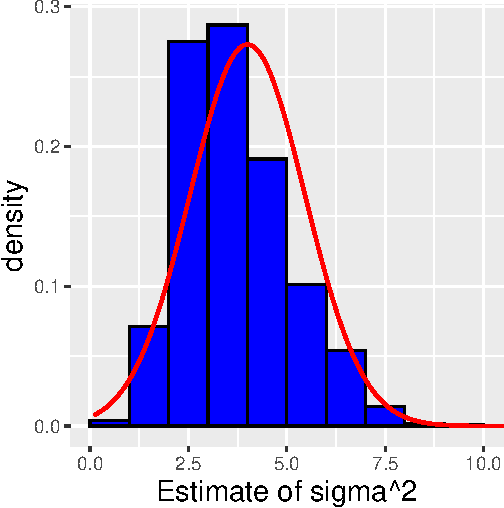
\includegraphics[keepaspectratio]{02-normal_files/figure-latex/fig-sigma2hatmlefig-1.pdf}}

}

\caption{\label{fig-sigma2hatmlefig}The empirical pdf for
\(\hat{\sigma^2}_{MLE}\) given \(n = 15\) and true variance
\(\sigma^2=4\). We overlay the asymptotic pdf in red.}

\end{figure}%

\begin{quote}
We see that if \(n\) is small, the distribution of the MLE for
\(\hat{\sigma^2}\) is definitely not normal, but right skew with a mean
smaller than the true mean (4) and standard deviation slightly smaller
than the true standard deviation (1.46).
\end{quote}

\section{Confidence Intervals}\label{sec-chap2confidence}

What to take away from this section:

\begin{itemize}
\item
  Given \(n\) iid data sampled according to a normal distribution, we
  can utilize numerical root-finding frameworks to construct
  \(100(1-\alpha)\)-percent confidence intervals for\ldots{}

  \begin{itemize}
  \item
    the normal population mean \(\mu\), if \(\sigma^2\) is known
    (utilizing the normal distribution);
  \item
    the normal population mean \(\mu\), if \(\sigma^2\) is unknown
    (utilizing the \(t\) distribution); and
  \item
    the normal population variance \(\sigma^2\) (utilizing the gamma
    distribution).
  \end{itemize}
\item
  Since the sampling distributions are continuous distributions, the
  interval coverage (i.e., the proportion of intervals that overlap the
  true value of \(\theta\)) is exactly \(1-\alpha\), as demonstrated via
  simulation.
\end{itemize}

For previous material on confidence intervals, see
Section~\ref{sec-chap1confidence}.

\smallskip\hrule

\begin{quote}
\textbf{Recall:} \emph{a confidence interval is a random interval
\([\hat{\theta}_L,\hat{\theta}_U]\) that overlaps (or covers) the true
value \(\theta\) with probability} \[
P\left( \hat{\theta}_L \leq \theta \leq \hat{\theta}_U \right) = 1 - \alpha \,,
\] \emph{where \(1 - \alpha\) is the confidence coefficient. Note that
this is a long-term probabilistic statement that is not to be applied to
any one numerically evaluated interval: an evaluated interval either
overlaps the true value, or it does not (and thus we cannot say there is
a \(100(1-\alpha)\)-percent chance that \(\theta\) lies within the
interval). We determine \(\hat{\theta}\) by solving the following
equation:} \[
F_Y(y_{\mathrm{obs}} \vert \theta) - q = 0 \,,
\] \emph{where \(F_Y(\cdot)\) is the cumulative distribution function
for the statistic \(Y\), \(y_{\mathrm{obs}}\) is the observed value of
the statistic, and \(q\) is an appropriate quantile value that is
determined using the confidence interval reference table introduced in
Section~\ref{sec-chap1confref}.}
\end{quote}

\smallskip\hrule

When we construct confidence intervals, we are allowed to utilize any
arbitrarily chosen statistic \(Y\), so long as we know its sampling
distribution and so long as \(Y\) is ``informative'' about \(\theta\).
(As an example of an uninformative statistic: given iid data sampled
according to a normal distribution, \(Y = S^2\) contains no information
that allows us to infer the value of the population mean, \(\mu\).)
However, in the context of the normal distribution, there are
conventional choices:

\begin{enumerate}
\def\labelenumi{\arabic{enumi}.}
\tightlist
\item
  When \(\theta = \mu\), and the variance \(\sigma^2\) is known, we use
  the sample mean \(\bar{X}\)
\item
  When \(\theta = \mu\), and the variance \(\sigma^2\) is unknown, we
  use \(T = (\bar{X}-\mu)/(S/\sqrt{n})\), where \(S\) is the sample
  standard deviation
\item
  When \(\theta = \sigma^2\), we use the sample variance \(S^2\)
\end{enumerate}

While these are conventional statistic choices, there are
well-established reasons for using them based on the idea of
\emph{interval length}: if we examine the use of two separate statistics
for constructing a confidence interval for \(\theta\), we generally want
to use the one that generates \emph{shorter confidence intervals} (i.e.,
the one that indicates the least amount of uncertainty about
\(\theta\)). And while we are not in a position to justify this
statement now, we can say that for normally distributed iid data,
\(\bar{X}\), \(T\), and \(S^2\) are the statistics that will generate
the shortest intervals. (Justification will come in
Section~\ref{sec-chap3nplemma} and Section~\ref{sec-chap4hypothesis}
when we discuss the Neyman-Pearson Lemma and the Likelihood Ratio Test.)

\subsection{Confidence Intervals: Numerical
Estimation}\label{sec-chap2confnum}

For the three cases stated above, we are not able to solve the equation
\(F_Y(y_{\mathrm{obs}} \vert \theta) - q = 0\) for \(\theta\) by hand.
But we need not worry: given \(y_{\mathrm{obs}}\) and that \(\theta\) is
continuously valued, there is a one-to-one relationship between
\(\theta\) and \(q\) and thus the equation will have only one root. We
can determine that root using a numerical root-finder such as
\texttt{R}'s \texttt{uniroot()} function. Here we show how to find
interval bounds for case 1; below, in examples, we provide similar code
snippets that cover cases 2 and 3.

Let's assume that we sample \(n = 25\) iid data according to a normal
distribution with variance \(\sigma^2 = 1\), and that we wish to
construct a 95\% two-sided confidence interval for \(\mu\).

\begin{Shaded}
\begin{Highlighting}[]
\CommentTok{\# generate data; typically, X would be provided}
\FunctionTok{set.seed}\NormalTok{(}\DecValTok{101}\NormalTok{)}
\NormalTok{n      }\OtherTok{\textless{}{-}} \DecValTok{25}
\NormalTok{sigma2 }\OtherTok{\textless{}{-}} \DecValTok{1}
\NormalTok{X      }\OtherTok{\textless{}{-}} \FunctionTok{rnorm}\NormalTok{(n, }\AttributeTok{mean =} \DecValTok{0}\NormalTok{, }\AttributeTok{sd =} \FunctionTok{sqrt}\NormalTok{(sigma2))}

\CommentTok{\# construct 95\% interval}
\NormalTok{alpha  }\OtherTok{\textless{}{-}} \FloatTok{0.05}
\NormalTok{Y      }\OtherTok{\textless{}{-}} \FunctionTok{mean}\NormalTok{(X)}

\NormalTok{f }\OtherTok{\textless{}{-}} \ControlFlowTok{function}\NormalTok{(mu, sigma2, n, y.obs, q)}
\NormalTok{\{}
  \FunctionTok{pnorm}\NormalTok{(y.obs, }\AttributeTok{mean =}\NormalTok{ mu, }\AttributeTok{sd =} \FunctionTok{sqrt}\NormalTok{(sigma2 }\SpecialCharTok{/}\NormalTok{ n)) }\SpecialCharTok{{-}}\NormalTok{ q  }\CommentTok{\# F\_Y(y\_obs | theta) {-} q}
\NormalTok{\}}

\CommentTok{\# lower bound: E[Y] = mu, so by table q = 1{-}alpha/2}
\FunctionTok{round}\NormalTok{(}\FunctionTok{uniroot}\NormalTok{(f, }\AttributeTok{interval =} \FunctionTok{c}\NormalTok{(}\SpecialCharTok{{-}}\DecValTok{10000}\NormalTok{, }\DecValTok{10000}\NormalTok{), }\AttributeTok{sigma2 =}\NormalTok{ sigma2, }\AttributeTok{n =}\NormalTok{ n,}
              \AttributeTok{y.obs =}\NormalTok{ Y, }\AttributeTok{q =} \DecValTok{1} \SpecialCharTok{{-}}\NormalTok{ alpha }\SpecialCharTok{/} \DecValTok{2}\NormalTok{)}\SpecialCharTok{$}\NormalTok{root, }\DecValTok{3}\NormalTok{)}
\end{Highlighting}
\end{Shaded}

\begin{verbatim}
[1] -0.488
\end{verbatim}

\begin{Shaded}
\begin{Highlighting}[]
\CommentTok{\# upper bound: E[Y] = mu, so by table q = alpha/2}
\FunctionTok{round}\NormalTok{(}\FunctionTok{uniroot}\NormalTok{(f, }\AttributeTok{interval =} \FunctionTok{c}\NormalTok{(}\SpecialCharTok{{-}}\DecValTok{10000}\NormalTok{, }\DecValTok{10000}\NormalTok{), }\AttributeTok{sigma2 =}\NormalTok{ sigma2, }\AttributeTok{n =}\NormalTok{ n,}
              \AttributeTok{y.obs =}\NormalTok{ Y, }\AttributeTok{q =}\NormalTok{     alpha }\SpecialCharTok{/} \DecValTok{2}\NormalTok{)}\SpecialCharTok{$}\NormalTok{root, }\DecValTok{3}\NormalTok{)}
\end{Highlighting}
\end{Shaded}

\begin{verbatim}
[1] 0.296
\end{verbatim}

The user-defined \texttt{f()} function evaluates
\(F_Y(y_{\mathrm{obs}} \vert \theta) - q\), given values for all three
quantities \(\theta = \mu\), \(y_{\mathrm{obs}}\), and \(q\), while the
function \texttt{uniroot()} varies \(\mu\) until \texttt{f()} returns a
value sufficiently close to zero. There are three aspects to this code
to immediately note. First, \texttt{R} will see that \texttt{mu} is the
only variable whose value is not fixed, and thus will automatically
search for the one value of \texttt{mu} such that
\(F_Y(y_{\mathrm{obs}} \vert \theta) - q = 0\) is satisfied (within
machine tolerance). Second, because \texttt{f()} requires other
quantities like \texttt{sigma2}, we must explicitly specify their values
in the calls to \texttt{uniroot()}. The third code aspect to note is the
argument \texttt{interval} that is passed to \texttt{uniroot()}. This is
the range of values of (in this case) \texttt{mu} over which \texttt{R}
will search for the one root. Since \(\mu\) can, in theory, take on any
value, we specify the interval as being from a very large negative
number to a very large positive number. Because \texttt{uniroot()}'s
root-finding algorithm is very robust and efficient, making the search
interval bounds inordinately large does not ultimately affect
performance: the roots will be found, and they will be found very
quickly. Here, we find that the interval is
\([\hat{\theta}_L,\hat{\theta}_U] =
[-0.488,0.296]\), which overlaps the true value. (See
Figure~\ref{fig-mukvarci}.)

\begin{figure}

\begin{minipage}[t]{0.50\linewidth}

\centering{

\pandocbounded{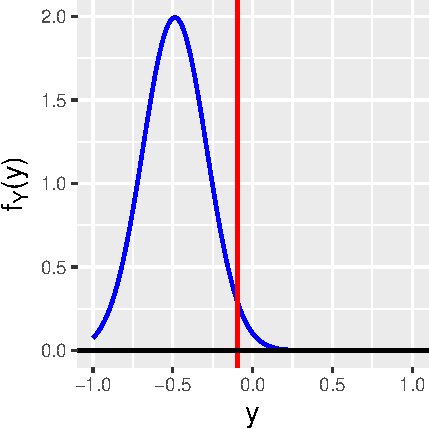
\includegraphics[keepaspectratio]{02-normal_files/figure-latex/fig-mukvarci-1.pdf}}

}

\subcaption{\label{fig-mukvarci-1}}

\end{minipage}%
%
\begin{minipage}[t]{0.50\linewidth}

\centering{

\pandocbounded{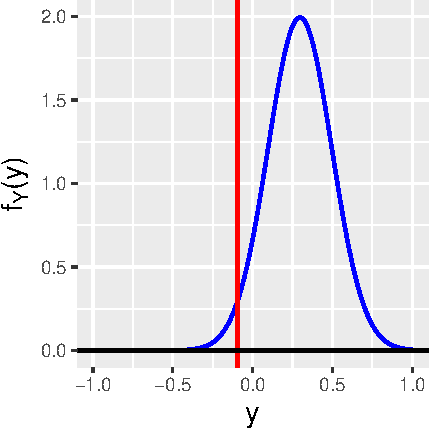
\includegraphics[keepaspectratio]{02-normal_files/figure-latex/fig-mukvarci-2.pdf}}

}

\subcaption{\label{fig-mukvarci-2}}

\end{minipage}%

\caption{\label{fig-mukvarci}Sampling distributions for
\(Y = \bar{X} = \sum_{i=1}^n X_i\), where \(n = 25\) and
\(X_i \sim \mathcal{N}(\mu,1)\), and where (a) \(\mu=-0.488\) and (b)
\(\mu=0.296\). We observe \(y_{\mathrm{obs}} = -0.0955\) and we want to
construct a 95\% confidence interval. \(\mu=-0.488\) is the smallest
value of \(\mu\) such that \(F_Y^{-1}(0.975) = -0.0955\), while
\(\mu=0.296\) is the largest value of \(\mu\) such that
\(F_Y^{-1}(0.025) = -0.0955\).}

\end{figure}%

To verify the ``coverage'' of the intervals we generate, i.e., to
determine the proportion of the intervals that overlap the true value,
we can simply wrap the code provided above with a \texttt{for} loop, and
save the lower and upper bounds for each generated dataset. (However, to
be clear: we can only estimate coverage via simulations if we know, or
assume, a value for \(\theta\).)

\begin{Shaded}
\begin{Highlighting}[]
\FunctionTok{set.seed}\NormalTok{(}\DecValTok{101}\NormalTok{)}
\NormalTok{num.sim }\OtherTok{\textless{}{-}} \DecValTok{10000}
\NormalTok{alpha   }\OtherTok{\textless{}{-}} \FloatTok{0.05}
\NormalTok{n       }\OtherTok{\textless{}{-}} \DecValTok{25}
\NormalTok{sigma2  }\OtherTok{\textless{}{-}} \DecValTok{1}
\NormalTok{lower   }\OtherTok{\textless{}{-}} \FunctionTok{rep}\NormalTok{(}\ConstantTok{NA}\NormalTok{, num.sim)}
\NormalTok{upper   }\OtherTok{\textless{}{-}} \FunctionTok{rep}\NormalTok{(}\ConstantTok{NA}\NormalTok{, num.sim)}

\NormalTok{f }\OtherTok{\textless{}{-}} \ControlFlowTok{function}\NormalTok{(mu, sigma2, n, y.obs, q)}
\NormalTok{\{}
  \FunctionTok{pnorm}\NormalTok{(y.obs, }\AttributeTok{mean =}\NormalTok{ mu, }\AttributeTok{sd =} \FunctionTok{sqrt}\NormalTok{(sigma2 }\SpecialCharTok{/}\NormalTok{ n)) }\SpecialCharTok{{-}}\NormalTok{ q}
\NormalTok{\}}

\ControlFlowTok{for}\NormalTok{ ( ii }\ControlFlowTok{in} \DecValTok{1}\SpecialCharTok{:}\NormalTok{num.sim ) \{}
\NormalTok{  X         }\OtherTok{\textless{}{-}} \FunctionTok{rnorm}\NormalTok{(n, }\AttributeTok{mean =} \DecValTok{0}\NormalTok{, }\AttributeTok{sd =} \FunctionTok{sqrt}\NormalTok{(sigma2))}
\NormalTok{  Y         }\OtherTok{\textless{}{-}} \FunctionTok{mean}\NormalTok{(X)}
\NormalTok{  lower[ii] }\OtherTok{\textless{}{-}} \FunctionTok{uniroot}\NormalTok{(f, }\AttributeTok{interval =} \FunctionTok{c}\NormalTok{(}\SpecialCharTok{{-}}\DecValTok{10000}\NormalTok{, }\DecValTok{10000}\NormalTok{), }\AttributeTok{sigma2 =}\NormalTok{ sigma2,}
                       \AttributeTok{n =}\NormalTok{ n, }\AttributeTok{y.obs =}\NormalTok{ Y, }\AttributeTok{q =} \DecValTok{1} \SpecialCharTok{{-}}\NormalTok{ alpha }\SpecialCharTok{/} \DecValTok{2}\NormalTok{)}\SpecialCharTok{$}\NormalTok{root}
\NormalTok{  upper[ii] }\OtherTok{\textless{}{-}} \FunctionTok{uniroot}\NormalTok{(f, }\AttributeTok{interval =} \FunctionTok{c}\NormalTok{(}\SpecialCharTok{{-}}\DecValTok{10000}\NormalTok{, }\DecValTok{10000}\NormalTok{), }\AttributeTok{sigma2 =}\NormalTok{ sigma2,}
                       \AttributeTok{n =}\NormalTok{ n, }\AttributeTok{y.obs =}\NormalTok{ Y, }\AttributeTok{q =}\NormalTok{     alpha }\SpecialCharTok{/} \DecValTok{2}\NormalTok{)}\SpecialCharTok{$}\NormalTok{root}
\NormalTok{\}}
\end{Highlighting}
\end{Shaded}

We can then see how often the true value is within the bounds:

\begin{Shaded}
\begin{Highlighting}[]
\NormalTok{truth    }\OtherTok{\textless{}{-}} \DecValTok{0}
\NormalTok{in.bound }\OtherTok{\textless{}{-}}\NormalTok{ (lower }\SpecialCharTok{\textless{}=}\NormalTok{ truth) }\SpecialCharTok{\&}\NormalTok{ (upper }\SpecialCharTok{\textgreater{}=}\NormalTok{ truth)}
\FunctionTok{cat}\NormalTok{(}\StringTok{"The empirical coverage is"}\NormalTok{, }\FunctionTok{sum}\NormalTok{(in.bound) }\SpecialCharTok{/}\NormalTok{ num.sim, }\StringTok{"}\SpecialCharTok{\textbackslash{}n}\StringTok{"}\NormalTok{)}
\end{Highlighting}
\end{Shaded}

\begin{verbatim}
The empirical coverage is 0.9518 
\end{verbatim}

Here, if \texttt{lower\ \textless{}=\ truth}, then \texttt{TRUE} is
returned, as is the case if \texttt{upper\ \textgreater{}=\ truth}.
\texttt{\&} is the logical \texttt{and} operator, which returns
\texttt{TRUE} if the input is \texttt{TRUE\ \&\ TRUE} and returns
\texttt{FALSE} otherwise. \texttt{R} treats \texttt{TRUE} as equivalent
to 1 (and \texttt{FALSE} as equivalent to 0), so \texttt{sum(in.bound)}
returns the number of final \texttt{TRUE} values, i.e., the number of
evaluated intervals that overlap the true value.

The estimated coverage is 0.9518. We do not expect a value of exactly
0.95 given that we only run a finite number of simulations and thus we
will observe random variation; however, we can say that this value is
``close'' to 0.95 and thus almost certainly compatible with 0.95. Once
we discuss the binomial distribution in Section~\ref{sec-chap3pmf}, we
will be able to more easily quantify the notion of being ``close'' to a
value we expect.

\begin{center}\rule{0.5\linewidth}{0.5pt}\end{center}

As this point, the reader may say, ``this doesn't look like the
confidence interval calculations that I learned in introductory
statistics.'' This observation is correct: calculations in introductory
statistics are done via formula and they ultimately rely on the use of
statistical tables. For instance, the reader may recall a formula like
this one: \[
\bar{X} \pm z_{1-\alpha/2} \frac{\sigma}{\sqrt{n}} \,,
\] where \(z_{1-\alpha/2} = \Phi^{-1}(1-\alpha/2)\) is a quantity that
one would look up using a \(z\) table. (For instance, for a 95\%
two-sided interval, one would determine that \(z_{0.975} = 1.96\).) For
the data generated in the example above, \(Y = \bar{X} = -0.0955\) and
the interval bounds are
\([\hat{\theta}_L,\hat{\theta}_U] = [-0.488,0.296]\)\ldots matching what
\texttt{uniroot()} found!

\emph{In the end, the use of numerical root-finders allows us to move
away from formulas (and the use of statistical tables) and to generalize
the process of calculating confidence intervals.}

For more on confidence intervals, go to
Section~\ref{sec-chap3confidence}.

\subsection{Examples}\label{examples-21}

\subsubsection{Normal Mean: Variance
Unknown}\label{normal-mean-variance-unknown}

\begin{quote}
Here, we assume the same setting as above, except that now the variance
is unknown.
\end{quote}

\begin{Shaded}
\begin{Highlighting}[]
\CommentTok{\# generate data}
\FunctionTok{set.seed}\NormalTok{(}\DecValTok{101}\NormalTok{)}
\NormalTok{alpha }\OtherTok{\textless{}{-}} \FloatTok{0.05}
\NormalTok{n     }\OtherTok{\textless{}{-}} \DecValTok{25}
\NormalTok{X     }\OtherTok{\textless{}{-}} \FunctionTok{rnorm}\NormalTok{(n, }\AttributeTok{mean =} \DecValTok{0}\NormalTok{, }\AttributeTok{sd =} \DecValTok{1}\NormalTok{)}

\CommentTok{\# construct 95\% interval}
\NormalTok{Y     }\OtherTok{\textless{}{-}} \FunctionTok{mean}\NormalTok{(X)}
\NormalTok{S2    }\OtherTok{\textless{}{-}} \FunctionTok{var}\NormalTok{(X)}

\NormalTok{f }\OtherTok{\textless{}{-}} \ControlFlowTok{function}\NormalTok{(mu, S2, n, y.obs, q)}
\NormalTok{\{}
  \FunctionTok{pt}\NormalTok{((y.obs }\SpecialCharTok{{-}}\NormalTok{ mu) }\SpecialCharTok{/} \FunctionTok{sqrt}\NormalTok{(S2 }\SpecialCharTok{/}\NormalTok{ n), n }\SpecialCharTok{{-}} \DecValTok{1}\NormalTok{) }\SpecialCharTok{{-}}\NormalTok{ q}
\NormalTok{\}}

\FunctionTok{round}\NormalTok{(}\FunctionTok{uniroot}\NormalTok{(f, }\AttributeTok{interval =} \FunctionTok{c}\NormalTok{(}\SpecialCharTok{{-}}\DecValTok{10000}\NormalTok{, }\DecValTok{10000}\NormalTok{), }\AttributeTok{S2 =}\NormalTok{ S2, }\AttributeTok{n =}\NormalTok{ n, }
              \AttributeTok{y.obs =}\NormalTok{ Y, }\AttributeTok{q =} \DecValTok{1} \SpecialCharTok{{-}}\NormalTok{ alpha }\SpecialCharTok{/} \DecValTok{2}\NormalTok{)}\SpecialCharTok{$}\NormalTok{root, }\DecValTok{3}\NormalTok{)}
\end{Highlighting}
\end{Shaded}

\begin{verbatim}
[1] -0.448
\end{verbatim}

\begin{Shaded}
\begin{Highlighting}[]
\FunctionTok{round}\NormalTok{(}\FunctionTok{uniroot}\NormalTok{(f, }\AttributeTok{interval =} \FunctionTok{c}\NormalTok{(}\SpecialCharTok{{-}}\DecValTok{10000}\NormalTok{, }\DecValTok{10000}\NormalTok{), }\AttributeTok{S2 =}\NormalTok{ S2, }\AttributeTok{n =}\NormalTok{ n,}
              \AttributeTok{y.obs =}\NormalTok{ Y, }\AttributeTok{q =}\NormalTok{     alpha }\SpecialCharTok{/} \DecValTok{2}\NormalTok{)}\SpecialCharTok{$}\NormalTok{root, }\DecValTok{3}\NormalTok{)}
\end{Highlighting}
\end{Shaded}

\begin{verbatim}
[1] 0.257
\end{verbatim}

\begin{quote}
The code above is largely equivalent to that in the previous example,
with the only changes being swapping in the call to \texttt{pt()} (and
altering the argument in that call) in place of the call to
\texttt{pnorm()}, and replacing the known value of \(\sigma^2\)
(\texttt{sigma2} in the previous example) with \(S^2\) (\texttt{S2}). We
find that the interval is \([\hat{\theta}_L,\hat{\theta}_U] =
[-0.448,0.257]\), which is similar to the interval derived in the last
example and which still overlaps the true value. (It is smaller than the
interval above because \(S^2 = 0.731 < 1\). See
Figure~\ref{fig-muuvarci}.)
\end{quote}

\begin{figure}

\begin{minipage}[t]{0.50\linewidth}

\centering{

\pandocbounded{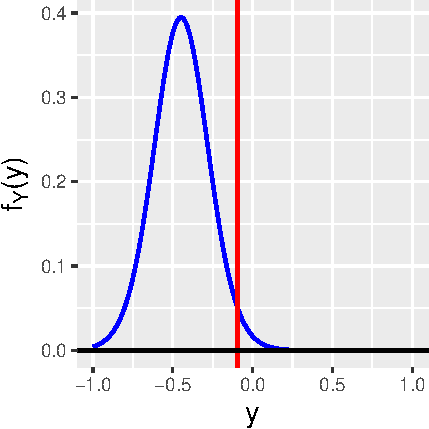
\includegraphics[keepaspectratio]{02-normal_files/figure-latex/fig-muuvarci-1.pdf}}

}

\subcaption{\label{fig-muuvarci-1}}

\end{minipage}%
%
\begin{minipage}[t]{0.50\linewidth}

\centering{

\pandocbounded{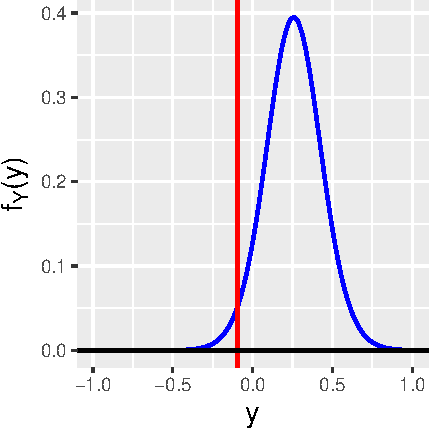
\includegraphics[keepaspectratio]{02-normal_files/figure-latex/fig-muuvarci-2.pdf}}

}

\subcaption{\label{fig-muuvarci-2}}

\end{minipage}%

\caption{\label{fig-muuvarci}Sampling distributions for \(Y = \bar{X}\),
where \(n = 25\) and \(X_i \sim \mathcal{N}(\mu,\sigma^2)\), and where
(a) \(\mu=-0.448\) and (b) \(\mu=0.257\). We observe
\(y_{\mathrm{obs}} = -0.0955\) and \(s_{\mathrm{obs}}^2 = 0.855\) and we
want to construct a 95\% confidence interval. \(\mu=-0.448\) is the
smallest value of \(\mu\) such that \(F_Y^{-1}(0.975) = -0.0955\), while
\(\mu=0.257\) is the largest value of \(\mu\) such that
\(F_Y^{-1}(0.025) = -0.0955\).}

\end{figure}%

\subsubsection{Normal Variance}\label{normal-variance}

\begin{quote}
Below, we adapt our confidence-interval code to the problem of
estimating an interval for the variance \(\sigma^2\).
\end{quote}

\begin{Shaded}
\begin{Highlighting}[]
\CommentTok{\# generate data}
\FunctionTok{set.seed}\NormalTok{(}\DecValTok{101}\NormalTok{)}
\NormalTok{alpha }\OtherTok{\textless{}{-}} \FloatTok{0.05}
\NormalTok{n     }\OtherTok{\textless{}{-}} \DecValTok{25}
\NormalTok{X     }\OtherTok{\textless{}{-}} \FunctionTok{rnorm}\NormalTok{(n, }\AttributeTok{mean =} \DecValTok{0}\NormalTok{, }\AttributeTok{sd =} \DecValTok{1}\NormalTok{)}

\CommentTok{\# construct 95\% interval}
\NormalTok{Y     }\OtherTok{\textless{}{-}} \FunctionTok{var}\NormalTok{(X)}

\NormalTok{f }\OtherTok{\textless{}{-}} \ControlFlowTok{function}\NormalTok{(sigma2, n, y.obs, q)}
\NormalTok{\{ }
  \FunctionTok{pgamma}\NormalTok{(y.obs, }\AttributeTok{shape =}\NormalTok{ (n }\SpecialCharTok{{-}} \DecValTok{1}\NormalTok{)}\SpecialCharTok{/}\DecValTok{2}\NormalTok{, }\AttributeTok{scale =} \DecValTok{2} \SpecialCharTok{*}\NormalTok{ sigma2 }\SpecialCharTok{/}\NormalTok{ (n }\SpecialCharTok{{-}} \DecValTok{1}\NormalTok{)) }\SpecialCharTok{{-}}\NormalTok{ q}
\NormalTok{\}}

\FunctionTok{round}\NormalTok{(}\FunctionTok{uniroot}\NormalTok{(f, }\AttributeTok{interval =} \FunctionTok{c}\NormalTok{(}\DecValTok{1}\NormalTok{.e}\DecValTok{{-}4}\NormalTok{, }\DecValTok{10000}\NormalTok{), }\AttributeTok{n =}\NormalTok{ n,}
              \AttributeTok{y.obs =} \FunctionTok{var}\NormalTok{(X), }\AttributeTok{q =} \DecValTok{1} \SpecialCharTok{{-}}\NormalTok{ alpha }\SpecialCharTok{/} \DecValTok{2}\NormalTok{)}\SpecialCharTok{$}\NormalTok{root, }\DecValTok{3}\NormalTok{)}
\end{Highlighting}
\end{Shaded}

\begin{verbatim}
[1] 0.445
\end{verbatim}

\begin{Shaded}
\begin{Highlighting}[]
\FunctionTok{round}\NormalTok{(}\FunctionTok{uniroot}\NormalTok{(f, }\AttributeTok{interval =} \FunctionTok{c}\NormalTok{(}\DecValTok{1}\NormalTok{.e}\DecValTok{{-}4}\NormalTok{, }\DecValTok{10000}\NormalTok{), }\AttributeTok{n =}\NormalTok{ n,}
              \AttributeTok{y.obs =} \FunctionTok{var}\NormalTok{(X), }\AttributeTok{q =}\NormalTok{     alpha }\SpecialCharTok{/} \DecValTok{2}\NormalTok{)}\SpecialCharTok{$}\NormalTok{root, }\DecValTok{3}\NormalTok{)}
\end{Highlighting}
\end{Shaded}

\begin{verbatim}
[1] 1.414
\end{verbatim}

\begin{quote}
The changes made to the code above include swapping in
\texttt{pgamma()}, removing the variable \texttt{mean}, removing the
variable \texttt{S2} (as \texttt{y.obs} itself is now \(S^2\)), and
adjusting the lower bound on the interval (since \(\sigma^2 > 0\)). We
find that the interval is
\([\widehat{\sigma}_L^2, \widehat{\sigma}_U^2] =
[0.445,1.414]\), which overlaps the true value. (See
Figure~\ref{fig-sigma2ci}.)
\end{quote}

\begin{figure}

\begin{minipage}[t]{0.50\linewidth}

\centering{

\pandocbounded{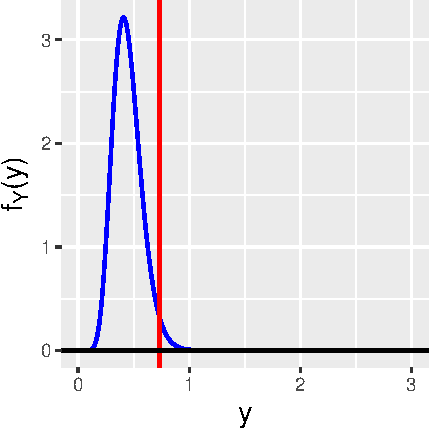
\includegraphics[keepaspectratio]{02-normal_files/figure-latex/fig-sigma2ci-1.pdf}}

}

\subcaption{\label{fig-sigma2ci-1}}

\end{minipage}%
%
\begin{minipage}[t]{0.50\linewidth}

\centering{

\pandocbounded{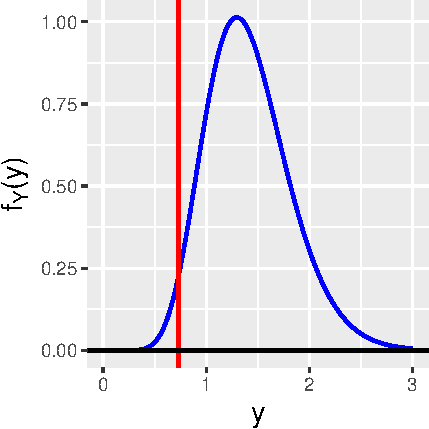
\includegraphics[keepaspectratio]{02-normal_files/figure-latex/fig-sigma2ci-2.pdf}}

}

\subcaption{\label{fig-sigma2ci-2}}

\end{minipage}%

\caption{\label{fig-sigma2ci}Sampling distributions for \(Y = S^2\),
where \(n = 25\) and \(X_i \sim \mathcal{N}(\mu,\sigma^2)\), and where
(a) \(\sigma^2=0.445\) and (b) \(\sigma^2=1.414\). We observe
\(y_{\mathrm{obs}} = s_{\mathrm{obs}}^2 = 0.731\) and we want to
construct a 95\% confidence interval. \(\sigma^2=0.445\) is the smallest
value of \(\sigma^2\) such that \(F_Y^{-1}(0.975) = 0.731\), while
\(\mu=1.414\) is the largest value of \(\sigma^2\) such that
\(F_Y^{-1}(0.025) = 0.731\).}

\end{figure}%

\subsubsection{Normal Mean: Leveraging the
CLT}\label{normal-mean-leveraging-the-clt}

\begin{quote}
Let's assume that we have a iid sample of \(n\) data drawn from the
distribution \[
f_X(x) = \theta x^{\theta-1} ~~~~ x \in [0,1] \,.
\] This distribution is decidedly \emph{not} normal. Can we derive a
confidence interval for the mean of this distribution, where the mean is
\[
E[X] = \int_0^1 \theta x x^{\theta-1} dx = \left. \frac{\theta}{\theta+1} x^{\theta+1} \right|_0^1 = \frac{\theta}{\theta+1} \,?
\] If we wanted to try to do this ``exactly,'' then one workflow would
be (a) to attempt to determine the sampling distribution of
\(Y = \bar{X}\) (utilizing, e.g., moment-generating functions), and then
(b) code up a variant of the codes given in the examples above. However,
regarding (a): the mgf of the distribution is \[
m_X(t) = E[e^{tX}] = \theta \int_0^1 x^{\theta-1} e^{tx} dx \,.
\] This looks suspiciously like a gamma-function integral, except the
bounds here are 0 and 1, not 0 and \(\infty\)\ldots what we actually
have (or, technically, what we would have after an appropriate variable
substitution) is an \emph{incomplete gamma function} integral. We cannot
easily work with this\ldots and so here we turn to the Central Limit
Theorem. (To be clear: here we will utilize the CLT simply to show how
it would be done. In any situation where the distribution for each of
the individual iid data is known or can be assumed, it is better to
utilize simulations and to construct confidence intervals using the
empirical sampling distribution, as this will provide an exactly correct
interval, within machine precision. We will carry out such simulations
starting in Section~\ref{sec-chap4confidence}.)
\end{quote}

\begin{quote}
If \(n \gtrsim 30\), we may write that \[
\bar{X} \overset{d}{\rightarrow} Y \sim \mathcal{N}(\mu,s_{\mathrm{obs}}^2/n) \,.
\] (Recall that the CLT assumes that we know \(\sigma^2\), but if we do
not and use \(S^2\) instead, the result will still hold as
\(n \rightarrow \infty\).) Thus we would use the confidence interval
approach that we describe in the first example above, while swapping in
\(s_{\mathrm{obs}}^2\) for \(\sigma^2\).
\end{quote}

\begin{Shaded}
\begin{Highlighting}[]
\CommentTok{\# generate data}
\FunctionTok{set.seed}\NormalTok{(}\DecValTok{101}\NormalTok{)}
\NormalTok{alpha }\OtherTok{\textless{}{-}} \FloatTok{0.05}
\NormalTok{n     }\OtherTok{\textless{}{-}} \DecValTok{25}
\NormalTok{theta }\OtherTok{\textless{}{-}} \DecValTok{2}   \CommentTok{\# so the mean is 2/3}
\NormalTok{X     }\OtherTok{\textless{}{-}} \FunctionTok{rbeta}\NormalTok{(n, theta, }\DecValTok{1}\NormalTok{)  }\CommentTok{\# theta x\^{}(theta{-}1) is a beta distribution}

\CommentTok{\# construct 95\% interval}
\NormalTok{Y     }\OtherTok{\textless{}{-}} \FunctionTok{mean}\NormalTok{(X)}
\NormalTok{S2    }\OtherTok{\textless{}{-}} \FunctionTok{var}\NormalTok{(X)}

\NormalTok{f }\OtherTok{\textless{}{-}} \ControlFlowTok{function}\NormalTok{(mu, S2, n, y.obs, q)}
\NormalTok{\{}
  \FunctionTok{pnorm}\NormalTok{(y.obs, }\AttributeTok{mean =}\NormalTok{ mu, }\AttributeTok{sd =} \FunctionTok{sqrt}\NormalTok{(S2 }\SpecialCharTok{/}\NormalTok{ n)) }\SpecialCharTok{{-}}\NormalTok{ q}
\NormalTok{\}}

\FunctionTok{round}\NormalTok{(}\FunctionTok{uniroot}\NormalTok{(f, }\AttributeTok{interval =} \FunctionTok{c}\NormalTok{(}\SpecialCharTok{{-}}\DecValTok{10000}\NormalTok{, }\DecValTok{10000}\NormalTok{), }\AttributeTok{S2 =}\NormalTok{ S2, }\AttributeTok{n =}\NormalTok{ n,}
              \AttributeTok{y.obs =}\NormalTok{ Y, }\AttributeTok{q =} \DecValTok{1} \SpecialCharTok{{-}}\NormalTok{ alpha }\SpecialCharTok{/} \DecValTok{2}\NormalTok{)}\SpecialCharTok{$}\NormalTok{root, }\DecValTok{3}\NormalTok{)}
\end{Highlighting}
\end{Shaded}

\begin{verbatim}
[1] 0.589
\end{verbatim}

\begin{Shaded}
\begin{Highlighting}[]
\FunctionTok{round}\NormalTok{(}\FunctionTok{uniroot}\NormalTok{(f, }\AttributeTok{interval =} \FunctionTok{c}\NormalTok{(}\SpecialCharTok{{-}}\DecValTok{10000}\NormalTok{, }\DecValTok{10000}\NormalTok{), }\AttributeTok{S2 =}\NormalTok{ S2, }\AttributeTok{n =}\NormalTok{ n,}
              \AttributeTok{y.obs =}\NormalTok{ Y, }\AttributeTok{q =}\NormalTok{     alpha }\SpecialCharTok{/} \DecValTok{2}\NormalTok{)}\SpecialCharTok{$}\NormalTok{root, }\DecValTok{3}\NormalTok{)}
\end{Highlighting}
\end{Shaded}

\begin{verbatim}
[1] 0.753
\end{verbatim}

\begin{quote}
The evaluated confidence interval is \([0.589, 0.753]\) (which overlaps
the true value \(\mu = 2/3\)). Note, however, that because an
approximate sampling distribution is being used, the coverage can (and
will) deviate from expectation (e.g., 0.95). Let's see how much the
coverage deviates in this one case via simulation:
\end{quote}

\begin{Shaded}
\begin{Highlighting}[]
\FunctionTok{set.seed}\NormalTok{(}\DecValTok{101}\NormalTok{)}
\NormalTok{alpha   }\OtherTok{\textless{}{-}} \FloatTok{0.05}
\NormalTok{num.sim }\OtherTok{\textless{}{-}} \DecValTok{10000}
\NormalTok{n       }\OtherTok{\textless{}{-}} \DecValTok{25}
\NormalTok{theta   }\OtherTok{\textless{}{-}} \DecValTok{2}
\NormalTok{lower   }\OtherTok{\textless{}{-}} \FunctionTok{rep}\NormalTok{(}\ConstantTok{NA}\NormalTok{, num.sim)}
\NormalTok{upper   }\OtherTok{\textless{}{-}} \FunctionTok{rep}\NormalTok{(}\ConstantTok{NA}\NormalTok{, num.sim)}

\NormalTok{f }\OtherTok{\textless{}{-}} \ControlFlowTok{function}\NormalTok{(mu, S2, n, y.obs, q)}
\NormalTok{\{}
  \FunctionTok{pnorm}\NormalTok{(y.obs, }\AttributeTok{mean =}\NormalTok{ mu, }\AttributeTok{sd =} \FunctionTok{sqrt}\NormalTok{(S2 }\SpecialCharTok{/}\NormalTok{ n)) }\SpecialCharTok{{-}}\NormalTok{ q}
\NormalTok{\}}

\ControlFlowTok{for}\NormalTok{ ( ii }\ControlFlowTok{in} \DecValTok{1}\SpecialCharTok{:}\NormalTok{num.sim ) \{}
\NormalTok{  X  }\OtherTok{\textless{}{-}} \FunctionTok{rbeta}\NormalTok{(n, theta, }\DecValTok{1}\NormalTok{)  }
\NormalTok{  Y  }\OtherTok{\textless{}{-}} \FunctionTok{mean}\NormalTok{(X)}
\NormalTok{  S2 }\OtherTok{\textless{}{-}} \FunctionTok{var}\NormalTok{(X)}
\NormalTok{  lower[ii] }\OtherTok{\textless{}{-}} \FunctionTok{uniroot}\NormalTok{(f, }\AttributeTok{interval =} \FunctionTok{c}\NormalTok{(}\SpecialCharTok{{-}}\DecValTok{10000}\NormalTok{, }\DecValTok{10000}\NormalTok{), }\AttributeTok{y.obs =}\NormalTok{ Y,}
                       \AttributeTok{S2 =}\NormalTok{ S2, }\AttributeTok{n =}\NormalTok{ n, }\AttributeTok{q =} \DecValTok{1} \SpecialCharTok{{-}}\NormalTok{ alpha }\SpecialCharTok{/} \DecValTok{2}\NormalTok{)}\SpecialCharTok{$}\NormalTok{root}
\NormalTok{  upper[ii] }\OtherTok{\textless{}{-}} \FunctionTok{uniroot}\NormalTok{(f, }\AttributeTok{interval =} \FunctionTok{c}\NormalTok{(}\SpecialCharTok{{-}}\DecValTok{10000}\NormalTok{, }\DecValTok{10000}\NormalTok{), }\AttributeTok{y.obs =}\NormalTok{ Y,}
                       \AttributeTok{S2 =}\NormalTok{ S2, }\AttributeTok{n =}\NormalTok{ n, }\AttributeTok{q =}\NormalTok{     alpha }\SpecialCharTok{/} \DecValTok{2}\NormalTok{)}\SpecialCharTok{$}\NormalTok{root}
\NormalTok{\}}

\NormalTok{truth    }\OtherTok{\textless{}{-}} \DecValTok{2}\SpecialCharTok{/}\DecValTok{3}
\NormalTok{in.bound }\OtherTok{\textless{}{-}}\NormalTok{ (lower }\SpecialCharTok{\textless{}=}\NormalTok{ truth) }\SpecialCharTok{\&}\NormalTok{ (upper }\SpecialCharTok{\textgreater{}=}\NormalTok{ truth)}
\FunctionTok{cat}\NormalTok{(}\StringTok{"The estimated coverage is "}\NormalTok{, }\FunctionTok{sum}\NormalTok{(in.bound) }\SpecialCharTok{/}\NormalTok{ num.sim, }\StringTok{"}\SpecialCharTok{\textbackslash{}n}\StringTok{"}\NormalTok{)}
\end{Highlighting}
\end{Shaded}

\begin{verbatim}
The estimated coverage is  0.9359 
\end{verbatim}

\begin{quote}
The estimated coverage is 0.936; it is not quite 0.95. Thus it appears
that our confidence interval does not have its advertised coverage. Note
that as \(n \rightarrow 0\), the coverage will deviate more and more
from \(1 - \alpha\), and that as \(n \rightarrow \infty\), the coverage
will asymptotically approach \(1 - \alpha\).
\end{quote}

\subsubsection{The Pivotal Method}\label{the-pivotal-method}

\begin{quote}
The pivotal method is an often-used analytical method for constructing
confidence intervals wherein one ``reformats'' the problem to solve in
such a way that one can ultimately utilize statistical tables to
determine interval bounds. In the age of computers, the pivotal method
has become unnecessary; the numerical root-finding algorithm presented
above constructs the same intervals (and does so even in situations
where the pivotal method cannot be used).
\end{quote}

\begin{quote}
The steps of the pivotal method are as follows:
\end{quote}

\begin{quote}
\begin{enumerate}
\def\labelenumi{\arabic{enumi}.}
\tightlist
\item
  Determine a pivotal quantity \(Y\), a statistic that is a function of
  both the observed data and the parameter \(\theta\), and that has a
  sampling distribution that does \emph{not} depend on \(\theta\). (Note
  that, as hinted at above, there is no guarantee that a pivotal
  quantity exists in any given situation. But there may also be
  situations where we can define multiple pivotal quantities; if so, it
  does not matter which we adopt, as they all will help generate the
  same interval.)
\item
  Determine constants \(a\) and \(b\) such that
  \(P(a \leq Y \leq b) = 1-\alpha\). (Here, we are assuming that we are
  constructing a two-sided interval.)
\item
  Rearrange the terms within the probability statement such that
  \(\theta\) is alone in the middle: the quantities on either end are
  the interval bounds.
\end{enumerate}
\end{quote}

\begin{quote}
Let's demonstrate how this plays out in the situation where we sample
\(n\) iid data from a normal distribution with known variance, and wish
to construct an interval for \(\mu\). As we know, in this situation, \[
\bar{X} \sim \mathcal{N}\left(\mu,\frac{\sigma^2}{n}\right) \,.
\] \(\bar{X}\) is \emph{not} a pivotal quantity: its sampling
distribution depends on \(\mu\). However\ldots{} \[
Y = \frac{\bar{X} - \mu}{\sigma/\sqrt{n}} \sim \mathcal{N}(0,1) 
\] \emph{is} a pivotal quantity, as it depends on both \(\bar{X}\)
\emph{and} \(\mu\) and has a sampling distribution that does \emph{not}
depend on \(\mu\). Thus step 1 is complete.
\end{quote}

\begin{quote}
As for step 2: \begin{align*}
P(a \leq Y \leq b) = P(Y \leq b) - P(Y \leq a) &= 1-\alpha \\
\Phi(b) - \Phi(a) &= 1-\alpha \,.
\end{align*} OK\ldots we appear stuck here, except that we can fall back
upon the fact that the standard normal distribution is symmetric around
zero, and thus we can say that \(a = -b\). That, and the fact that
symmetry allows us to write that \(\Phi(-b) = 1 - \Phi(b)\), allows us
to continue: \begin{align*}
\Phi(b) - \Phi(a) &= 1-\alpha \\
\Phi(b) - (1 - \Phi(b)) &= 1-\alpha \\
2\Phi(b) - 1 &= 1-\alpha \\
\Phi(b) &= \frac{2-\alpha}{2} = 1 - \frac{\alpha}{2} \\
b &= \Phi^{-1}\left(1 - \frac{\alpha}{2}\right) = z_{1-\alpha/2} \\
\end{align*} Historically, at this point, one would make use of a \(z\)
table to determine that, e.g., \(b = z_{0.975} = 1.96\).
\end{quote}

\begin{quote}
So now we move on to step 3: \begin{align*}
P\left(-z_{1-\alpha/2} \leq Y \leq z_{1-\alpha/2}\right) = P\left(-z_{1-\alpha/2} \leq \frac{\bar{X} - \mu}{\sigma/\sqrt{n}} \leq z_{1-\alpha/2}\right) &= 1-\alpha \\
\Rightarrow P\left(\bar{X} - z_{1-\alpha/2}\frac{\sigma}{\sqrt{n}} \leq \mu \leq \bar{X} + z_{1-\alpha/2}\frac{\sigma}{\sqrt{n}}\right) &= 1-\alpha \,.
\end{align*} Thus our confidence interval is \[
\bar{x}_{\mathrm{obs}} \pm z_{1-\alpha/2}\frac{\sigma}{\sqrt{n}} \,.
\]
\end{quote}

\begin{quote}
Ultimately, the pivotal method adds an extra step to our confidence
interval estimation framework, as shown in Figure~\ref{fig-pivotal}.
\end{quote}

\begin{figure}

\centering{

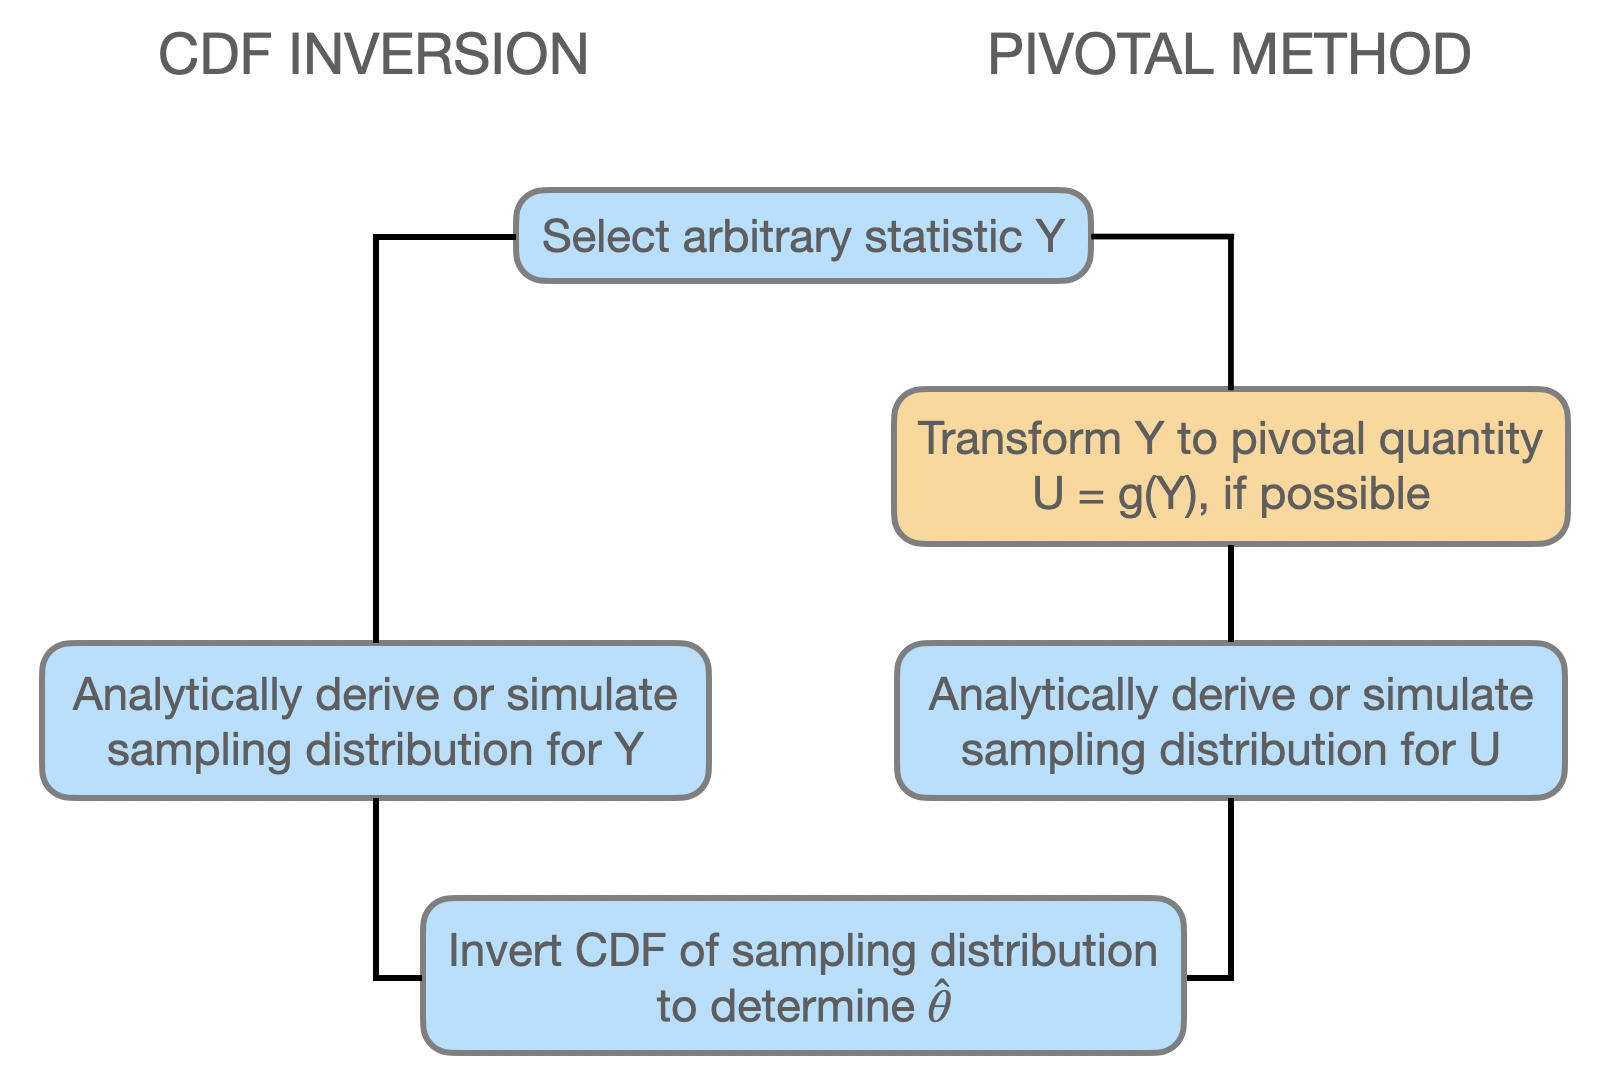
\includegraphics[width=0.75\linewidth,height=\textheight,keepaspectratio]{figures/pivotal.png}

}

\caption{\label{fig-pivotal}Workflows for generating confidence interval
estimates using the method introduced in
Section~\ref{sec-chap1confidence} (here, dubbed cdf inversion) and the
pivotal method. In both methods, we begin by selecting an arbitrary
statistic \(Y\) and we finish by determining a sampling distribution and
inverting the cdf of that distribution to determine \(\hat{\theta}\).
The pivotal method simply adds the step of determining a pivotal
quantity, which ultimately allows solutions to be determined via the use
of statistical tables. From Freeman (2026).}

\end{figure}%

\section{Hypothesis Testing}\label{sec-chap2hypothesis}

What to take away from this section:

\begin{itemize}
\item
  Given \(n\) iid data sampled according to a normal distribution, we
  can utilize pre-coded \texttt{R} functions to test hypotheses
  about\ldots{}

  \begin{itemize}
  \item
    the normal population mean \(\mu\), if \(\sigma^2\) is known
    (utilizing the normal distribution);
  \item
    the normal population mean \(\mu\), if \(\sigma^2\) is unknown
    (utilizing the \(t\) distribution); and
  \item
    the normal population variance \(\sigma^2\) (utilizing the gamma
    distribution).
  \end{itemize}
\item
  The \emph{rejection region} associated with a hypothesis test is the
  set of values along the real-number line: if the observed hypothesis
  test statistic value \(y_{\mathrm{obs}}\) lies in this set, then we
  \emph{reject the null hypothesis}.
\item
  The \emph{power} of a test is the probability that we would reject the
  null hypothesis given an arbitrary value for \(\theta\); if
  \(\theta = \theta_o\), the null hypothesis value, the test power is
  the test level \(\alpha\) (e.g., 0.05) by definition.
\end{itemize}

For previous material on hypothesis testing, see
Section~\ref{sec-chap1hypothesis}.

\smallskip\hrule

\begin{quote}
\textbf{Recall}: \emph{a hypothesis test is a framework for deciding
whether a specific value of a population parameter \(\theta\) is
plausible, given the data that we observe. The null hypothesis \(H_o\)
is \(\theta = \theta_o\), while possible alternatives \(H_a\) are
\(\theta \neq \theta_o\) (two-tail test), \(\theta > \theta_o\)
(upper-tail test), and \(\theta < \theta_o\) (lower-tail test). The
\(p\)-value is the probability of observing a statistic value
\(y_{\mathrm{obs}}\) or a more extreme value, relative to the null. We
reject the null hypothesis if the \(p\)-value is less than the stated
test level \(\alpha\); otherwise, we fail to reject the null.}
\end{quote}

\smallskip\hrule

Let's assume we are given \(n\) iid data \(\{X_1,\ldots,X_n\}\) sampled
according to a normal distribution. As was the case when constructing
confidence intervals, there are conventional choices for the statistics
we would use to infer the population mean \(\mu\) and/or variance
\(\sigma^2\):

\begin{enumerate}
\def\labelenumi{\arabic{enumi}.}
\tightlist
\item
  When \(\theta = \mu\), and the variance \(\sigma^2\) is known, we use
  the sample mean \(\bar{X}\)
\item
  When \(\theta = \mu\), and the variance \(\sigma^2\) is unknown, we
  use \(T = (\bar{X}-\mu)/(S/\sqrt{n})\), where \(S\) is the sample
  standard deviation
\item
  When \(\theta = \sigma^2\), we use the sample variance \(S^2\)
\end{enumerate}

We can use the hypothesis test reference table provided in
Section~\ref{sec-chap1hypref} to compute \(p\)-values in each of these
situations, noting that because \(E[\bar{X}]\) and \(E[S^2]\) increase
with \(\mu\) and \(\sigma^2\), respectively, we always utilize formulas
on the ``yes'' lines of the table.

Before we transition to examples, there are two new
hypothesis-test-related concepts that we will introduce here: \emph{test
power} and \emph{rejection regions}.

\subsection{Hypothesis Testing: Test Power}\label{sec-chap2power}

In words, test power is the probability of rejecting the null hypothesis
given an arbitrary parameter value \(\theta\): \[
\mbox{power}(\theta) = P(\mbox{reject}~H_o \vert \theta) \,.
\] The power is a function of \(\theta\), and its value is
\(1-\beta(\theta,\alpha)\), where \(\beta(\theta,\alpha)\) is the Type
II error. A \emph{power curve} is an often-used visualization that
indicates how power varies as a function of \(\theta\), with all other
quantities (the sample size \(n\), the null hypothesis value
\(\theta_o\), etc.) remaining fixed. An example for a two-tail test is
shown in Figure~\ref{fig-zpowcurve}. This figure shows how if we set
\(\theta = \theta_o\), the null hypothesis value, then the power will by
definition be \(\alpha\) (the probability of rejecting the null if the
null is indeed correct). To increase the test power (e.g., to make the
curve thinner and sharper in Figure~\ref{fig-zpowcurve}), we would
increase the sample size. There are two other things to note about power
curves: (1) the minimum power value for a two-tail test will be less
than \(\alpha\) if we are working with a sampling distribution that has
an asymmetric probability density or mass function, and (2) while it is
convention to only show power curves to the relevant side of the null in
one-tail tests, we can compute power for \emph{all} values of
\(\theta\); such curves will monotonically rise from 0 to 1 (upper-tail
tests) or descend from 1 to 0 (lower-tail tests).

\subsection{Hypothesis Testing: Rejection Regions}\label{sec-chap2rr}

Before we can compute test power, however, we need to first determine
those values of \(Y\) for which we would reject the null hypothesis,
i.e., we need to determine the \emph{rejection region} boundary or
boundaries associated with the test. To show how we would do this, we
will start with a statement: if our observed statistic value is equal to
a rejection-region boundary value, i.e., if
\(y_{\mathrm{obs}} = y_{\mathrm{RR}}\), then the observed \(p\)-value
will be exactly equal to \(\alpha\) (assuming our sampling distribution
is continuous\ldots we will defer our discussion of what happens with
discrete sampling distributions to Section~\ref{sec-chap3hypdisc}).
Combining the above statement with the hypothesis test reference table
given in Section~\ref{sec-chap1hypref}, we can, e.g., write the
following for a lower-tail/``yes''-line test: \[
p = F_Y(y_{\mathrm{obs}} \vert \theta_o) ~~~ \Rightarrow ~~~ \alpha = F_Y(y_{\mathrm{RR}} \vert \theta_o) ~~~ \Rightarrow ~~~ y_{\mathrm{RR}} = F_Y^{-1}(\alpha \vert \theta_o) \,.
\] In other words, the computation of a rejection-region boundary is a
straightforward inverse cdf calculation, which we can perform
analytically or by using a \texttt{R} code such as \texttt{qnorm()}.

It is important to note that the computation of rejection region
boundaries and test power do \emph{not} depend on what we observe when
we carry out an experiment, i.e., they do not depend on
\(y_{\mathrm{obs}}\). This is important: for instance, given specified
null and alternative hypotheses, we can determine the sample size we
would need in order to achieve a stated power before data are ever
collected! We show an example of such a sample-size calculation below.

\subsection{Hypothesis Testing: Power and Rejection Region Reference
Table}\label{sec-chap2hypref}

Below, we provide a second hypothesis test reference table, one that
contains details on the computations that one needs to compute rejection
regions and test power. Like the table in Section~\ref{sec-chap1hypref},
this is \emph{not} a table to memorize, but rather to refer back to when
solving problems!

{\def\LTcaptype{none} % do not increment counter
\begin{longtable}[]{@{}
  >{\raggedleft\arraybackslash}p{(\linewidth - 6\tabcolsep) * \real{0.1892}}
  >{\raggedleft\arraybackslash}p{(\linewidth - 6\tabcolsep) * \real{0.1892}}
  >{\centering\arraybackslash}p{(\linewidth - 6\tabcolsep) * \real{0.3784}}
  >{\centering\arraybackslash}p{(\linewidth - 6\tabcolsep) * \real{0.2432}}@{}}
\toprule\noalign{}
\begin{minipage}[b]{\linewidth}\raggedleft
Type
\end{minipage} & \begin{minipage}[b]{\linewidth}\raggedleft
\(E[Y]\) Increases with \(\theta\)?
\end{minipage} & \begin{minipage}[b]{\linewidth}\centering
Rejection Region(s)
\end{minipage} & \begin{minipage}[b]{\linewidth}\centering
Test Power
\end{minipage} \\
\midrule\noalign{}
\endhead
\bottomrule\noalign{}
\endlastfoot
two-tail & N/A &
\(\{y_{\mathrm{obs}} : y_{\mathrm{obs}} < y_{\mathrm{RR,lo}} = F_Y^{-1}(\alpha/2 \vert \theta_o)\}\)
and & \(F_Y(y_{\mathrm{RR,lo}} \vert \theta) +\) \\
& &
\(\{y_{\mathrm{obs}} : y_{\mathrm{obs}} > y_{\mathrm{RR,hi}} = F_Y^{-1}(1-\alpha/2 \vert \theta_o)\}\)
& \(1 - F_Y(y_{\mathrm{RR,hi}} \vert \theta)\) \\
lower-tail & yes &
\(\{y_{\mathrm{obs}} : y_{\mathrm{obs}} < y_{\mathrm{RR}} = F_Y^{-1}(\alpha \vert \theta_o)\}\)
& \(F_Y(y_{\mathrm{RR}} \vert \theta)\) \\
& no &
\(\{y_{\mathrm{obs}} : y_{\mathrm{obs}} > y_{\mathrm{RR}} = F_Y^{-1}(1-\alpha \vert \theta_o)\}\)
& \(1-F_Y(y_{\mathrm{RR}} \vert \theta)\) \\
upper-tail & yes &
\(\{y_{\mathrm{obs}} : y_{\mathrm{obs}} < y_{\mathrm{RR}} = F_Y^{-1}(1-\alpha \vert \theta_o)\}\)
& \(1-F_Y(y_{\mathrm{RR}} \vert \theta)\) \\
& no &
\(\{y_{\mathrm{obs}} : y_{\mathrm{obs}} > y_{\mathrm{RR}} = F_Y^{-1}(\alpha \vert \theta_o)\}\)
& \(F_Y(y_{\mathrm{RR}} \vert \theta)\) \\
\end{longtable}
}

We illustrate how to utilize this table in examples below.

For more on hypothesis testing, go to Section~\ref{sec-chap3nplemma} and
Section~\ref{sec-chap3categorical}.

\subsection{Examples}\label{examples-22}

\subsubsection{Normal Mean: Variance
Known}\label{normal-mean-variance-known}

\begin{quote}
Let's assume that we have sampled \(n = 25\) iid data from a normal
distribution whose variance is \(\sigma^2 = 1\). We wish to test the
null hypothesis \(H_o : \mu = \mu_o = 2\) versus the alternative
\(H_a : \mu \neq \mu_o\). What is the \(p\)-value if we observe
\(\bar{x}_{\mathrm{obs}} = 1.404\)? What is the power of this test for
\(\mu = 1.8\)? We assume the level of the test is \(\alpha = 0.05\).
\end{quote}

\begin{quote}
To answer each of these questions, we will refer to the hypothesis test
reference tables given in Section~\ref{sec-chap1hypref} and above.
\end{quote}

\begin{quote}
First, we compute the \(p\)-value. We utilize the table in
Section~\ref{sec-chap1hypref} and write down the following code.
\end{quote}

\begin{Shaded}
\begin{Highlighting}[]
\NormalTok{n      }\OtherTok{\textless{}{-}} \DecValTok{25}
\NormalTok{y.obs  }\OtherTok{\textless{}{-}} \FloatTok{1.404}
\NormalTok{mu.o   }\OtherTok{\textless{}{-}} \DecValTok{2}
\NormalTok{sigma2 }\OtherTok{\textless{}{-}} \DecValTok{1}
\DecValTok{2} \SpecialCharTok{*} \FunctionTok{min}\NormalTok{(}\FunctionTok{c}\NormalTok{(    }\FunctionTok{pnorm}\NormalTok{(y.obs, }\AttributeTok{mean =}\NormalTok{ mu.o, }\AttributeTok{sd =} \FunctionTok{sqrt}\NormalTok{(sigma2 }\SpecialCharTok{/}\NormalTok{ n)),}
          \DecValTok{1} \SpecialCharTok{{-}} \FunctionTok{pnorm}\NormalTok{(y.obs, }\AttributeTok{mean =}\NormalTok{ mu.o, }\AttributeTok{sd =} \FunctionTok{sqrt}\NormalTok{(sigma2 }\SpecialCharTok{/}\NormalTok{ n))))}
\end{Highlighting}
\end{Shaded}

\begin{verbatim}
[1] 0.002882484
\end{verbatim}

\begin{quote}
The \(p\)-value is 0.0029. This value is to be interpreted as the
probability that we would observe a value as far or farther from 2 as
1.404 (and 2.596, by symmetry) is 0.29 percent, if the null is correct.
As \(p < \alpha\), we reject the null hypothesis and conclude that the
true value of \(\mu\) is not equal to 2.
\end{quote}

\begin{quote}
To compute the test power, we start by determining the two rejection
region boundaries: \[
y_{\mathrm{RR,lo}} = F_Y^{-1}\left(\frac{\alpha}{2} \vert \mu_o\right) ~~~ \mbox{and} ~~~ y_{\mathrm{RR,hi}} = F_Y^{-1}\left(1-\frac{\alpha}{2} \vert \mu_o\right) \,,
\] where \(Y = \bar{X}\). The \texttt{R} function calls are
\end{quote}

\begin{Shaded}
\begin{Highlighting}[]
\NormalTok{n        }\OtherTok{\textless{}{-}} \DecValTok{25}
\NormalTok{alpha    }\OtherTok{\textless{}{-}} \FloatTok{0.05}
\NormalTok{mu.o     }\OtherTok{\textless{}{-}} \DecValTok{2}
\NormalTok{sigma2   }\OtherTok{\textless{}{-}} \DecValTok{1}
\NormalTok{(y.rr.lo }\OtherTok{\textless{}{-}} \FunctionTok{qnorm}\NormalTok{(    alpha}\SpecialCharTok{/}\DecValTok{2}\NormalTok{, }\AttributeTok{mean =}\NormalTok{ mu.o, }\AttributeTok{sd =} \FunctionTok{sqrt}\NormalTok{(sigma2 }\SpecialCharTok{/}\NormalTok{ n)))}
\end{Highlighting}
\end{Shaded}

\begin{verbatim}
[1] 1.608007
\end{verbatim}

\begin{Shaded}
\begin{Highlighting}[]
\NormalTok{(y.rr.hi }\OtherTok{\textless{}{-}} \FunctionTok{qnorm}\NormalTok{(}\DecValTok{1} \SpecialCharTok{{-}}\NormalTok{ alpha}\SpecialCharTok{/}\DecValTok{2}\NormalTok{, }\AttributeTok{mean =}\NormalTok{ mu.o, }\AttributeTok{sd =} \FunctionTok{sqrt}\NormalTok{(sigma2 }\SpecialCharTok{/}\NormalTok{ n)))}
\end{Highlighting}
\end{Shaded}

\begin{verbatim}
[1] 2.391993
\end{verbatim}

\begin{quote}
In any experiment in which we sample 25 data from a normal distribution
with mean \(\mu = 2\) and variance \(\sigma^2 = 1\), we would reject the
null hypothesis if \(y_{\mathrm{obs}}\) (the sample mean) is less than
1.608 or greater than 2.392. See Figure~\ref{fig-normex1}, where the
rejection regions are displayed in red. To compute the test power, we
plug \(y_{\mathrm{RR,lo}}\) and \(y_{\mathrm{RR,hi}}\) into the formula
given in the table above:
\end{quote}

\begin{Shaded}
\begin{Highlighting}[]
\NormalTok{n      }\OtherTok{\textless{}{-}} \DecValTok{25}
\NormalTok{alpha  }\OtherTok{\textless{}{-}} \FloatTok{0.05}
\NormalTok{mu.o   }\OtherTok{\textless{}{-}} \DecValTok{2}
\NormalTok{mu     }\OtherTok{\textless{}{-}} \FloatTok{1.8}
\NormalTok{sigma2 }\OtherTok{\textless{}{-}} \DecValTok{1}
     \FunctionTok{pnorm}\NormalTok{(y.rr.lo, }\AttributeTok{mean =}\NormalTok{ mu, }\AttributeTok{sd =} \FunctionTok{sqrt}\NormalTok{(sigma2 }\SpecialCharTok{/}\NormalTok{ n)) }\SpecialCharTok{+} 
\NormalTok{(}\DecValTok{1} \SpecialCharTok{{-}} \FunctionTok{pnorm}\NormalTok{(y.rr.hi, }\AttributeTok{mean =}\NormalTok{ mu, }\AttributeTok{sd =} \FunctionTok{sqrt}\NormalTok{(sigma2 }\SpecialCharTok{/}\NormalTok{ n)))}
\end{Highlighting}
\end{Shaded}

\begin{verbatim}
[1] 0.170075
\end{verbatim}

\begin{quote}
The test power is 0.170. \emph{If} \(\mu\) is actually equal to 1.8,
then 17.0 percent of the time that we sample 25 data, we would reject
the null.
\end{quote}

\begin{figure}

\centering{

\pandocbounded{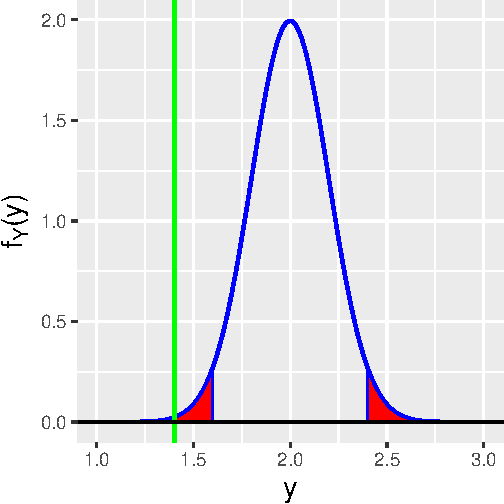
\includegraphics[keepaspectratio]{02-normal_files/figure-latex/fig-normex1-1.pdf}}

}

\caption{\label{fig-normex1}The sampling distribution
\(f_Y(y \vert \mu)\) (blue curve), rejection regions (red polygons), and
observed statistic value \(y_{\mathrm{obs}}\) (vertical green line) for
\(Y = \bar{X}\) given \(n = 25\) iid data that are assumed to be sampled
according to a \(\mathcal{N}(2,1)\) distribution under the null
hypothesis. We perform a two-tailed test, with \(\alpha = 0.05\), and
the variance \(\sigma^2 = 1\) is assumed known. The value we observe is
in the rejection region, thus we reject the null hypothesis and conclude
that \(\mu \neq 2\).}

\end{figure}%

\begin{figure}

\centering{

\pandocbounded{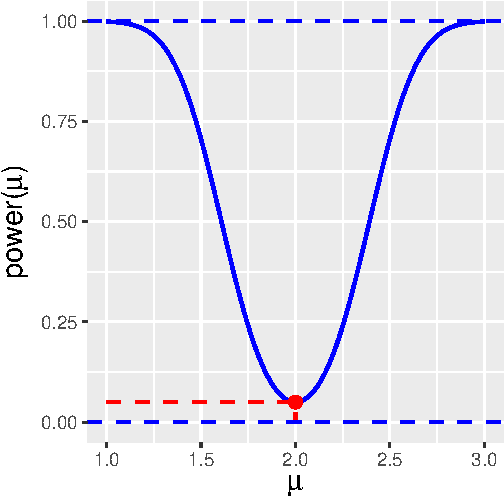
\includegraphics[keepaspectratio]{02-normal_files/figure-latex/fig-zpowcurve-1.pdf}}

}

\caption{\label{fig-zpowcurve}The power curve for the two-tail test
\(H_o : \mu = \mu_o = 2\) versus \(H_a : \mu \neq \mu_o\). The red dot
at \(\mu = 2\) indicates the test power under the null: the power is
\(\alpha\), as it should be given the definition of test power. We see
that \(n = 25\) is a sufficient amount of data to clearly disambiguate
between \(\mu_o = 2\) and, e.g., \(\mu \gtrsim 3\).}

\end{figure}%

\subsubsection{Normal Mean: Estimating Sample Size with Variance
Known}\label{normal-mean-estimating-sample-size-with-variance-known}

\begin{quote}
We can phrase a typical experimental design exercise as follows. ``We
will sample data according to a normal distribution with specified mean
\(\mu\) and specified variance \(\sigma^2\).'' (Alternatively, it could
be a specification of \(s_{\mathrm{obs}}^2\), motivating the use of
\(t\) distribution.) ``How many data do we need to collect to achieve a
test power of 0.8, assuming \(\alpha = 0.05\) and assuming that the null
hypothesis is \(H_o : \mu = \mu_o\), but the true value is
\(\mu > \mu_o\)?''
\end{quote}

\begin{quote}
We will begin answering this question using math, and later we will
transition to code.
\end{quote}

\begin{quote}
We refer back to the hypothesis test reference tables and note that for
an upper-tail test where \(E[Y]\) increases with \(\theta\), \[
\mbox{power}(\theta) = 1 - F_Y(y_{\mathrm{RR}} \vert \mu_o) \,.
\] We substitute in our target power value and solve for \(n\):
\begin{align*}
1 - F_Y(y_{\mathrm{RR}} \vert \mu_o) &= 0.8 \\
\Rightarrow ~~~ F_Y(y_{\mathrm{RR}} \vert \mu_o) &= 0.2 \\
\Rightarrow ~~~ &\mbox{...?} \,.
\end{align*} We transition here to code. We refer back to the hypothesis
test reference tables and note that for an upper-tail/``yes''-line test,
\(y_{\mathrm{RR}}\) is
\end{quote}

\begin{Shaded}
\begin{Highlighting}[]
\NormalTok{y.rr }\OtherTok{\textless{}{-}} \FunctionTok{qnorm}\NormalTok{(}\DecValTok{1} \SpecialCharTok{{-}}\NormalTok{ alpha }\SpecialCharTok{/} \DecValTok{2}\NormalTok{, }\AttributeTok{mean =}\NormalTok{ mu.o, }\AttributeTok{sd =} \FunctionTok{sqrt}\NormalTok{(sigma2 }\SpecialCharTok{/}\NormalTok{ n))}
\end{Highlighting}
\end{Shaded}

\begin{quote}
while the test power is given by
\end{quote}

\begin{Shaded}
\begin{Highlighting}[]
\DecValTok{1} \SpecialCharTok{{-}} \FunctionTok{pnorm}\NormalTok{(y.rr, }\AttributeTok{mean =}\NormalTok{ mu, }\AttributeTok{sd =} \FunctionTok{sqrt}\NormalTok{(sigma2 }\SpecialCharTok{/}\NormalTok{ n))}
\end{Highlighting}
\end{Shaded}

\begin{quote}
To solve the problem at hand, we would subtract 0.8 from this
expression, set the result equal to zero, and utilize \texttt{uniroot()}
to solve for \(n\):
\end{quote}

\begin{Shaded}
\begin{Highlighting}[]
\NormalTok{alpha  }\OtherTok{\textless{}{-}} \FloatTok{0.05}
\NormalTok{mu.o   }\OtherTok{\textless{}{-}} \DecValTok{8}
\NormalTok{mu     }\OtherTok{\textless{}{-}} \DecValTok{9}
\NormalTok{sigma2 }\OtherTok{\textless{}{-}} \DecValTok{6}

\NormalTok{f }\OtherTok{\textless{}{-}} \ControlFlowTok{function}\NormalTok{(n)}
\NormalTok{\{}
\NormalTok{  y.rr }\OtherTok{\textless{}{-}} \FunctionTok{qnorm}\NormalTok{(}\DecValTok{1} \SpecialCharTok{{-}}\NormalTok{ alpha}\SpecialCharTok{/}\DecValTok{2}\NormalTok{, }\AttributeTok{mean =}\NormalTok{ mu.o, }\AttributeTok{sd =} \FunctionTok{sqrt}\NormalTok{(sigma2 }\SpecialCharTok{/}\NormalTok{ n))}
  \FunctionTok{pnorm}\NormalTok{(y.rr, }\AttributeTok{mean =}\NormalTok{ mu, }\AttributeTok{sd =} \FunctionTok{sqrt}\NormalTok{(sigma2 }\SpecialCharTok{/}\NormalTok{ n)) }\SpecialCharTok{{-}} \FloatTok{0.2}
\NormalTok{\}}

\FunctionTok{ceiling}\NormalTok{(}\FunctionTok{uniroot}\NormalTok{(f, }\AttributeTok{interval =} \FunctionTok{c}\NormalTok{(}\DecValTok{1}\NormalTok{, }\DecValTok{1000}\NormalTok{))}\SpecialCharTok{$}\NormalTok{root)}
\end{Highlighting}
\end{Shaded}

\begin{verbatim}
[1] 48
\end{verbatim}

\begin{quote}
To achieve a power of 0.8, we would need to collect a sample of \(n=48\)
data. Note how we use the function \texttt{ceiling()} here, which rounds
up the result to the next higher integer. We do this because the sample
size should be an integer, and because we want the power to be \emph{at
least} 0.8; if we round our result down (via the \texttt{floor()}
function), the power will be less than 0.8. \emph{In sample
size-determination exercises, always round the final result up!}
\end{quote}

\subsubsection{Normal Mean: Variance
Unknown}\label{normal-mean-variance-unknown-1}

\begin{quote}
Let's assume that we have sampled \(n = 15\) iid data from a normal
distribution whose variance is unknown. We wish to test the null
hypothesis \(H_o : \mu = \mu_o = 4\) versus the alternative
\(H_a : \mu > \mu_o\). What is the \(p\)-value if we observe
\(\bar{x}_{\mathrm{obs}} = 4.5\)? What is the power of this test for
\(\mu = 4.5\)? We assume the level of the test is \(\alpha = 0.05\) and
that the sample variance is \(s_{\mathrm{obs}}^2 = 3\).
\end{quote}

\begin{quote}
To answer each of these questions, we will refer to the hypothesis test
reference tables given in Section~\ref{sec-chap1hypref} and above.
\end{quote}

\begin{quote}
First, we compute the \(p\)-value. We refer to the hypothesis test table
in Section~\ref{sec-chap1hypref} and write down the following:
\end{quote}

\begin{Shaded}
\begin{Highlighting}[]
\NormalTok{n      }\OtherTok{\textless{}{-}} \DecValTok{15}
\NormalTok{mu.o   }\OtherTok{\textless{}{-}} \DecValTok{4}
\NormalTok{s2.obs }\OtherTok{\textless{}{-}} \DecValTok{3}
\NormalTok{y.obs  }\OtherTok{\textless{}{-}}\NormalTok{ (}\FloatTok{4.5} \SpecialCharTok{{-}}\NormalTok{ mu.o) }\SpecialCharTok{/} \FunctionTok{sqrt}\NormalTok{(s2.obs }\SpecialCharTok{/}\NormalTok{ n)}
\DecValTok{1} \SpecialCharTok{{-}} \FunctionTok{pt}\NormalTok{(y.obs, n }\SpecialCharTok{{-}} \DecValTok{1}\NormalTok{)}
\end{Highlighting}
\end{Shaded}

\begin{verbatim}
[1] 0.1411855
\end{verbatim}

\begin{quote}
The \(p\)-value is 0.141, which is \(> \alpha\). The probability that we
would observe a value as far or farther from 4 as 4.5 is 14.1 percent,
if the null is correct. We thus fail to reject the null hypothesis; we
conclude that we have insufficient statistical evidence to reject the
idea that \(\mu = 4\).
\end{quote}

\begin{quote}
Now we would compute the test power\ldots except that for this
particular test, our two-step prescription of ``determine the rejection
region boundary and then use it to directly calculate the power'' will
not work in the way it did in the example above (and the way it does in
general). This is because the location and shape of a \(t\) distribution
depends only on the sample size \(n\); if we only change \(\mu_o\) to
\(\mu\), the probability density function will not move relative to the
rejection-region boundary. Thus we need more information to attack power
calculation for \(t\) tests.
\end{quote}

\begin{quote}
Recall that if we are given two random variables,
\(Z \sim \mathcal{N}(0,1)\) and \(W \sim \chi_{\nu}^2\), then
\(T = Z/\sqrt{W/\nu}\) is a \(t\)-distributed random variable for
\(\nu\) degrees of freedom. In a similar vein, \[
T_\delta = \frac{Z + \delta}{\sqrt{W/\nu}}
\] is a random variable that is sampled according to a \emph{non-central
t distribution} for \(\nu\) degrees of freedom, with the
\emph{non-centrality parameter} \(\delta\). In a \(t\)-test power
calculation, the non-centrality parameter, or ncp, is \[
\delta = \frac{\mu - \mu_o}{\sigma/\sqrt{n}} \,.
\] We notice right away that this parameter includes \(\sigma\), whose
value is unknown. (If we did know it, we would not be performing a \(t\)
test in the first place!) In place of \(\sigma\), we can use \(S\), or
more precisely, \[
S' = \frac{\Gamma((n-1)/2)}{\Gamma(n/2)} \sqrt{\frac{n-1}{2}} S \,,
\] since as shown in an example in Section~\ref{sec-chap2variance},
\(E[S'] = \sigma\). In the end, we cannot specify the power for a \(t\)
test \emph{exactly}; we can only estimate it.
\end{quote}

\begin{quote}
Below, we carry out the power calculation: we first determine the
rejection-region boundary (as before) and then plug the result into the
cumulative distribution function for a non-central \(t\) distribution,
as opposed to a central one.
\end{quote}

\begin{Shaded}
\begin{Highlighting}[]
\NormalTok{n       }\OtherTok{\textless{}{-}} \DecValTok{15}
\NormalTok{mu.o    }\OtherTok{\textless{}{-}} \DecValTok{4}
\NormalTok{mu      }\OtherTok{\textless{}{-}} \FloatTok{4.5}
\NormalTok{s       }\OtherTok{\textless{}{-}} \FunctionTok{sqrt}\NormalTok{(}\DecValTok{3}\NormalTok{)}
\NormalTok{s.prime }\OtherTok{\textless{}{-}}\NormalTok{ s }\SpecialCharTok{*} \FunctionTok{gamma}\NormalTok{((n }\SpecialCharTok{{-}} \DecValTok{1}\NormalTok{) }\SpecialCharTok{/} \DecValTok{2}\NormalTok{) }\SpecialCharTok{*} \FunctionTok{sqrt}\NormalTok{((n }\SpecialCharTok{{-}} \DecValTok{1}\NormalTok{) }\SpecialCharTok{/} \DecValTok{2}\NormalTok{) }\SpecialCharTok{/} \FunctionTok{gamma}\NormalTok{(n }\SpecialCharTok{/} \DecValTok{2}\NormalTok{)}
\NormalTok{delta   }\OtherTok{\textless{}{-}}\NormalTok{ (mu }\SpecialCharTok{{-}}\NormalTok{ mu.o) }\SpecialCharTok{/}\NormalTok{ (s.prime }\SpecialCharTok{/} \FunctionTok{sqrt}\NormalTok{(n))}

\NormalTok{y.rr }\OtherTok{\textless{}{-}} \FunctionTok{qt}\NormalTok{(}\DecValTok{1} \SpecialCharTok{{-}}\NormalTok{ alpha, n }\SpecialCharTok{{-}} \DecValTok{1}\NormalTok{)}
\DecValTok{1} \SpecialCharTok{{-}} \FunctionTok{pt}\NormalTok{(y.rr, n }\SpecialCharTok{{-}} \DecValTok{1}\NormalTok{, delta)}
\end{Highlighting}
\end{Shaded}

\begin{verbatim}
[1] 0.2744317
\end{verbatim}

\begin{quote}
We estimate the test power to be 0.274: \emph{if} \(\mu\) is equal to
4.5, then approximately 27.4 percent of the time we would sample a value
\(y_{\mathrm{obs}}\) that lies in the rejection region. The farther
\(\mu\) is from \(\mu_o\) (in the positive direction), the higher this
percentage gets. See Figure~\ref{fig-varpowcurve}.
\end{quote}

\begin{figure}

\centering{

\pandocbounded{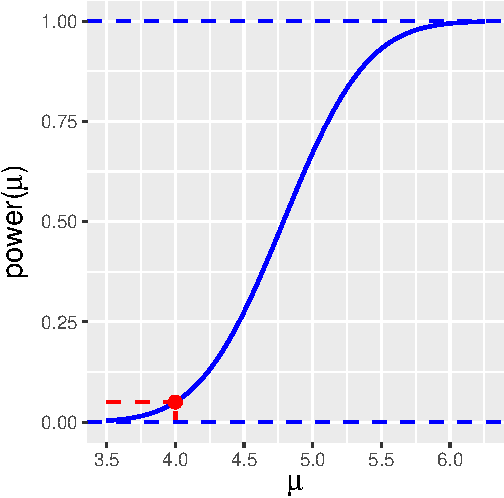
\includegraphics[keepaspectratio]{02-normal_files/figure-latex/fig-varpowcurve-1.pdf}}

}

\caption{\label{fig-varpowcurve}The power curve for the upper-tail test
\(H_o : \mu = \mu_o = 4\) versus \(H_a : \mu > \mu_o\). The red dot at
\(\mu = 4\) indicates the test power under the null: the power is
\(\alpha\), as it should be given the definition of test power. We see
that \(n = 15\) is a sufficient amount of data to clearly disambiguate
between \(\mu_o = 4\) and, e.g., \(\mu \gtrsim 5\). We note that if the
alternative hypothesis is \(\mu < \mu_o\), the curve would be
reversed\(-\)it would rise towards the left\(-\)and if the alternative
hypothesis is \(\mu \neq \mu_o\), the power curve would have a U shape,
with the minimum power being \(\alpha\) at \(\mu = \mu_o\).}

\end{figure}%

\subsubsection{Normal Variance}\label{normal-variance-1}

\begin{quote}
Let's assume that we have sampled \(n = 14\) iid data from a normal
distribution of unknown mean and variance. We wish to test the null
hypothesis \(H_o : \sigma^2 = \sigma_o^2 = 4\) versus the alternative
\(H_a : \sigma^2 > \sigma_o^2\). What is the \(p\)-value if we observe
\(s_{\mathrm{obs}}^2 = 5.5\)? What is the power of this test if
\(\sigma^2 = 8\)? To answer each of these questions, we utilize the
hypothesis test reference tables. We assume the level of the test is
\(\alpha = 0.05\).
\end{quote}

\begin{quote}
The relevant code for the \(p\)-value is
\end{quote}

\begin{Shaded}
\begin{Highlighting}[]
\NormalTok{y.obs    }\OtherTok{\textless{}{-}} \FloatTok{5.5}
\NormalTok{n        }\OtherTok{\textless{}{-}} \DecValTok{14}
\NormalTok{sigma2.o }\OtherTok{\textless{}{-}} \DecValTok{4}
\DecValTok{1} \SpecialCharTok{{-}} \FunctionTok{pgamma}\NormalTok{(y.obs, }\AttributeTok{shape =}\NormalTok{ (n }\SpecialCharTok{{-}} \DecValTok{1}\NormalTok{) }\SpecialCharTok{/} \DecValTok{2}\NormalTok{, }\AttributeTok{scale =} \DecValTok{2} \SpecialCharTok{*}\NormalTok{ sigma2.o }\SpecialCharTok{/}\NormalTok{ (n }\SpecialCharTok{{-}} \DecValTok{1}\NormalTok{))}
\end{Highlighting}
\end{Shaded}

\begin{verbatim}
[1] 0.1623236
\end{verbatim}

\begin{quote}
The \(p\)-value is 0.162, which is indeed \(> \alpha\). There is thus a
16.2 percent chance that we would sample a variance value of 5.5 or
greater if the null is correct. This is too high a percentage for us to
confidently reject the idea that \(\sigma^2 = 4\).
\end{quote}

\begin{quote}
To compute test power, we first determine the rejection region boundary.
The \texttt{R} function call is
\end{quote}

\begin{Shaded}
\begin{Highlighting}[]
\NormalTok{alpha }\OtherTok{\textless{}{-}} \FloatTok{0.05}
\NormalTok{(y.rr }\OtherTok{\textless{}{-}} \FunctionTok{qgamma}\NormalTok{(}\DecValTok{1} \SpecialCharTok{{-}}\NormalTok{ alpha, }\AttributeTok{shape =}\NormalTok{ (n }\SpecialCharTok{{-}} \DecValTok{1}\NormalTok{) }\SpecialCharTok{/} \DecValTok{2}\NormalTok{, }\AttributeTok{scale =} \DecValTok{2} \SpecialCharTok{*}\NormalTok{ sigma2.o }\SpecialCharTok{/}\NormalTok{ (n }\SpecialCharTok{{-}} \DecValTok{1}\NormalTok{)))}
\end{Highlighting}
\end{Shaded}

\begin{verbatim}
[1] 6.880625
\end{verbatim}

\begin{quote}
The boundary is \(y_{\mathrm{RR}} = 6.881\). With that number in hand,
we can compute the power assuming \(\sigma^2 = 8\):
\end{quote}

\begin{Shaded}
\begin{Highlighting}[]
\NormalTok{sigma2 }\OtherTok{\textless{}{-}} \DecValTok{8}
\DecValTok{1} \SpecialCharTok{{-}} \FunctionTok{pgamma}\NormalTok{(y.rr, }\AttributeTok{shape =}\NormalTok{ (n }\SpecialCharTok{{-}} \DecValTok{1}\NormalTok{) }\SpecialCharTok{/} \DecValTok{2}\NormalTok{, }\AttributeTok{scale =} \DecValTok{2} \SpecialCharTok{*}\NormalTok{ sigma2 }\SpecialCharTok{/}\NormalTok{ (n }\SpecialCharTok{{-}} \DecValTok{1}\NormalTok{))}
\end{Highlighting}
\end{Shaded}

\begin{verbatim}
[1] 0.5956563
\end{verbatim}

\begin{quote}
The power is 0.596: \emph{if} \(\sigma^2\) is equal to 8, then 59.6
percent of the time we would sample a value of \(y_{\mathrm{obs}}\) that
lies in the rejection region. This is not a particularly high value; if
being able to differentiate between \(\sigma_o^2 = 4\) and
\(\sigma^2 = 8\) is an important research goal, we would want to collect
more data!
\end{quote}

\begin{quote}
Below, we plot test power for this example versus sample size. Because
we are not solving for \(n\) given a particular power value, there is no
need to utilize \texttt{uniroot()}; we simply need to loop over calls to
\texttt{qgamma()} and \texttt{pgamma()}. (But note that we don't
actually ``loop,'' as \texttt{R}'s vectorization capabilities allow us
to simply pass vectors of sample-size values into the function calls,
with vectors of results being returned.) See Figure~\ref{fig-varpow2}.
\end{quote}

\begin{Shaded}
\begin{Highlighting}[]
\NormalTok{alpha    }\OtherTok{\textless{}{-}} \FloatTok{0.05}
\NormalTok{sigma2.o }\OtherTok{\textless{}{-}} \DecValTok{4}
\NormalTok{sigma2   }\OtherTok{\textless{}{-}} \DecValTok{8}
\NormalTok{n        }\OtherTok{\textless{}{-}} \DecValTok{2}\SpecialCharTok{:}\DecValTok{100}
\NormalTok{y.rr     }\OtherTok{\textless{}{-}} \FunctionTok{qgamma}\NormalTok{(}\DecValTok{1} \SpecialCharTok{{-}}\NormalTok{ alpha, }\AttributeTok{shape =}\NormalTok{ (n }\SpecialCharTok{{-}} \DecValTok{1}\NormalTok{) }\SpecialCharTok{/} \DecValTok{2}\NormalTok{, }\AttributeTok{scale =} \DecValTok{2} \SpecialCharTok{*}\NormalTok{ sigma2.o }\SpecialCharTok{/}\NormalTok{ (n }\SpecialCharTok{{-}} \DecValTok{1}\NormalTok{))}
\NormalTok{power    }\OtherTok{\textless{}{-}} \DecValTok{1} \SpecialCharTok{{-}} \FunctionTok{pgamma}\NormalTok{(y.rr, }\AttributeTok{shape =}\NormalTok{ (n }\SpecialCharTok{{-}} \DecValTok{1}\NormalTok{) }\SpecialCharTok{/} \DecValTok{2}\NormalTok{, }\AttributeTok{scale =} \DecValTok{2} \SpecialCharTok{*}\NormalTok{ sigma2 }\SpecialCharTok{/}\NormalTok{ (n }\SpecialCharTok{{-}} \DecValTok{1}\NormalTok{))}
\end{Highlighting}
\end{Shaded}

\begin{figure}

\centering{

\pandocbounded{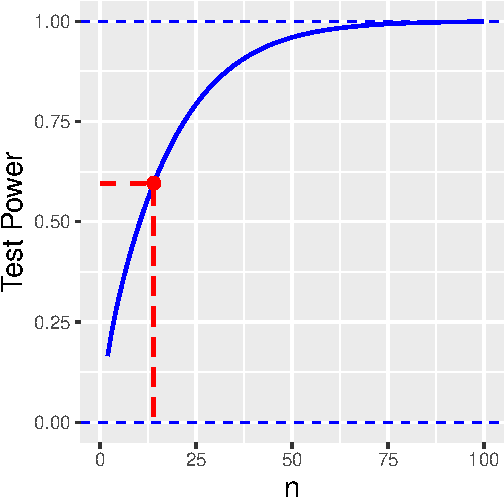
\includegraphics[keepaspectratio]{02-normal_files/figure-latex/fig-varpow2-1.pdf}}

}

\caption{\label{fig-varpow2}The test power as a function of sample size
\(n\) assuming \(\sigma_o^2 = 4\), \(\sigma^2 = 8\), and
\(\alpha = 0.05\). The red dot indicates the test power for \(n = 14\),
which as shown in the text is 0.596.}

\end{figure}%

\subsubsection{Normal Mean: Leveraging the
CLT}\label{normal-mean-leveraging-the-clt-1}

\begin{quote}
Let's go back to the example in the confidence interval section above,
in which we worked with \(n\) iid data from the decidedly not-normal
distribution \[
f_X(x) = \theta x^{\theta-1} ~~ x \in [0,1] \,,
\] with \(\theta > 0\). For this distribution,
\(E[X] = \mu = \theta/(\theta+1)\). We found that because we cannot
express the sampling distribution of \(Y = \bar{X}\) analytically, our
only path to determining a confidence interval was by making use of the
Central Limit Theorem.
\end{quote}

\begin{quote}
To determine \(p\)-value and test power, we would utilize the codes
shown for the ``variance known'' case above (i.e., the ones based on
\texttt{pnorm()} and \texttt{qnorm()}). However, instead of plugging in
\(\sigma^2\) (i.e., \texttt{sigma2}), we would plug in the sample
variance \(s_{\mathrm{obs}}^2\) (i.e., \texttt{s2.obs}). For instance,
if we assume that we have sampled \(n = 15\) data according to the
distribution above, with \(\bar{x}_{\mathrm{obs}} = 0.65\) and
\(s_{\mathrm{obs}}^2 = 0.01\), and we wish to test \(H_o : \mu = 0.6\)
versus \(H_a : \mu > 0.6\) at the level \(\alpha = 0.05\), the
\(p\)-value is given by
\end{quote}

\begin{Shaded}
\begin{Highlighting}[]
\NormalTok{n      }\OtherTok{\textless{}{-}} \DecValTok{15}
\NormalTok{alpha  }\OtherTok{\textless{}{-}} \FloatTok{0.05}
\NormalTok{mu.o   }\OtherTok{\textless{}{-}} \FloatTok{0.6}
\NormalTok{s2.obs }\OtherTok{\textless{}{-}} \FloatTok{0.01}
\NormalTok{y.obs  }\OtherTok{\textless{}{-}} \FloatTok{0.65}
\DecValTok{1} \SpecialCharTok{{-}} \FunctionTok{pnorm}\NormalTok{(y.obs, }\AttributeTok{mean =}\NormalTok{ mu.o, }\AttributeTok{sd =} \FunctionTok{sqrt}\NormalTok{(s2.obs }\SpecialCharTok{/}\NormalTok{ n))}
\end{Highlighting}
\end{Shaded}

\begin{verbatim}
[1] 0.02640376
\end{verbatim}

\begin{quote}
Since \(p < \alpha\), we reject the null hypothesis and conclude that we
have sufficient statistical evidence to state that the population mean
\(\mu\) is greater than 0.6.
\end{quote}

\begin{quote}
We note that, as is the case for confidence interval coverage, our
result is only approximate, i.e., the Type I error rate is not exactly
\(\alpha\), because the distribution of \(\bar{X}\) is not exactly
normal. However, as we do in the confidence interval case, we can
perform simulations to assess just how far off our actual Type I error
rate \(\alpha\) is for any given analysis setting.
\end{quote}

\begin{Shaded}
\begin{Highlighting}[]
\FunctionTok{set.seed}\NormalTok{(}\DecValTok{101}\NormalTok{)}
\NormalTok{num.sim  }\OtherTok{\textless{}{-}} \DecValTok{10000}    \CommentTok{\# repeat the data{-}generating process 10,000 times}
\NormalTok{n        }\OtherTok{\textless{}{-}} \DecValTok{15}
\NormalTok{alpha    }\OtherTok{\textless{}{-}} \FloatTok{0.05}
\NormalTok{mu.o     }\OtherTok{\textless{}{-}} \FloatTok{0.6}
\NormalTok{typeIErr }\OtherTok{\textless{}{-}} \DecValTok{0}
\ControlFlowTok{for}\NormalTok{ ( ii }\ControlFlowTok{in} \DecValTok{1}\SpecialCharTok{:}\NormalTok{num.sim ) \{}
\NormalTok{  X       }\OtherTok{\textless{}{-}} \FunctionTok{rbeta}\NormalTok{(n, mu.o }\SpecialCharTok{/}\NormalTok{ (}\DecValTok{1} \SpecialCharTok{{-}}\NormalTok{ mu.o), }\DecValTok{1}\NormalTok{)}
\NormalTok{  y.obs   }\OtherTok{\textless{}{-}} \FunctionTok{mean}\NormalTok{(X)}
\NormalTok{  s2.obs  }\OtherTok{\textless{}{-}} \FunctionTok{var}\NormalTok{(X)}
\NormalTok{  y.rr.lo }\OtherTok{\textless{}{-}} \FunctionTok{qnorm}\NormalTok{(  alpha }\SpecialCharTok{/} \DecValTok{2}\NormalTok{, }\AttributeTok{mean =}\NormalTok{ mu.o, }\AttributeTok{sd =} \FunctionTok{sqrt}\NormalTok{(s2.obs }\SpecialCharTok{/}\NormalTok{ n))}
\NormalTok{  y.rr.hi }\OtherTok{\textless{}{-}} \FunctionTok{qnorm}\NormalTok{(}\DecValTok{1}\SpecialCharTok{{-}}\NormalTok{alpha }\SpecialCharTok{/} \DecValTok{2}\NormalTok{, }\AttributeTok{mean =}\NormalTok{ mu.o, }\AttributeTok{sd =} \FunctionTok{sqrt}\NormalTok{(s2.obs }\SpecialCharTok{/}\NormalTok{ n))}
  \ControlFlowTok{if}\NormalTok{ ( y.obs }\SpecialCharTok{\textless{}=}\NormalTok{ y.rr.lo }\SpecialCharTok{||}\NormalTok{ y.obs }\SpecialCharTok{\textgreater{}=}\NormalTok{ y.rr.hi ) typeIErr }\OtherTok{=}\NormalTok{ typeIErr }\SpecialCharTok{+} \DecValTok{1}
\NormalTok{\}}
\FunctionTok{cat}\NormalTok{(}\StringTok{"The observed proportion of Type I errors ="}\NormalTok{, typeIErr }\SpecialCharTok{/}\NormalTok{ num.sim, }\StringTok{"}\SpecialCharTok{\textbackslash{}n}\StringTok{"}\NormalTok{)}
\end{Highlighting}
\end{Shaded}

\begin{verbatim}
The observed proportion of Type I errors = 0.0737 
\end{verbatim}

\begin{quote}
We observe an empirical Type I error rate of 0.0737. This is
sufficiently far from the value we expect, \(\alpha = 0.05\), that we
can conclude that when we draw \(n = 15\) data from the distribution
given above, the sampling distribution of the mean is still only
approximately normal.
\end{quote}

\subsubsection{Normal Mean: Two-Sample
Testing}\label{normal-mean-two-sample-testing}

\begin{quote}
Let's assume that we are given two independent samples of normal iid
data: \begin{align*}
\{U_1,\ldots,U_{n_U}\} &\sim \mathcal{N}(\mu_U,\sigma_U^2) \\
\{V_1,\ldots,V_{n_V}\} &\sim \mathcal{N}(\mu_V,\sigma_V^2) \,.
\end{align*} The sample means are \(\bar{U}\) and \(\bar{V}\),
respectively, and we know that \[
\bar{U} \sim \mathcal{N}\left(\mu_U,\frac{\sigma_U^2}{n_U}\right) ~~\mbox{and}~~ \bar{V} \sim \mathcal{N}\left(\mu_V,\frac{\sigma_V^2}{n_V}\right) \,.
\] In a \emph{two-sample t test}, the hypotheses being examined are,
typically, \(H_o : \mu_U = \mu_V\) and \(H_a : \mu_U \neq \mu_V\). Thus
a natural test statistic is \(\bar{U}-\bar{V}\), which, as the reader
may confirm using the method of moment-generating functions, is itself
normally distributed: \[
\bar{U} - \bar{V} \sim \mathcal{N}\left(\mu_U-\mu_V,\frac{\sigma_U^2}{n_U}+\frac{\sigma_V^2}{n_V}\right) \,.
\] However, when neither variance is known, we cannot model the observed
data with the normal distribution; instead, in \emph{Welch's t} test, we
assume the following: \[
T = \frac{\bar{U}-\bar{V}}{S_\Delta} = \frac{\bar{U}-\bar{V}}{\sqrt{\frac{S_U^2}{n_U}+\frac{S_V^2}{n_V}}} \sim t_{\nu} \,,
\] i.e., \(T\) is sampled according to a \(t\) distribution with \(\nu\)
degrees of freedom, where \(\nu\) is estimated using the
Welch-Satterthwaite equation: \[
\nu \approx \frac{S_\Delta^4}{\frac{S_U^4}{n_U^2(n_U-1)} + \frac{S_V^4}{n_V^2(n_V-1)}} \,.
\] The rule-of-thumb for this approximation to hold is that both \(n_U\)
and \(n_V\) need to be larger than 5. Note that in some applications,
one might see \(\nu\) rounded off to an integer, but this is not
necessary: one can work with the \(t\) distribution's probability
density function just fine even if \(\nu\) in not an integer! (Any
rounding off is done to allow one to use \(t\) tables to estimate
\(p\)-values.)
\end{quote}

\begin{quote}
Can we ``reformat'' this test so as to be consistent with how we perform
one-sample tests? The answer is yes. Let the test statistic be
\(Y = \bar{U}-\bar{V} = S_{\Delta} T\), and let the null hypothesis be
\(H_o : \mu_U - \mu_V = 0\). Then \[
F_Y(y) = P(Y \leq y) = P(S_{\Delta} T \leq y) = P\left(T \leq \frac{y}{S_{\Delta}}\right) = F_{T}\left(\frac{y}{S_{\Delta}}\right) \,,
\] and thus the \(p\)-value is given by
\end{quote}

\begin{Shaded}
\begin{Highlighting}[]
\NormalTok{p     }\OtherTok{\textless{}{-}} \DecValTok{2} \SpecialCharTok{*} \FunctionTok{min}\NormalTok{(}\FunctionTok{c}\NormalTok{(}\FunctionTok{pt}\NormalTok{(y.obs }\SpecialCharTok{/}\NormalTok{ S.Delta, nu), }\DecValTok{1} \SpecialCharTok{{-}} \FunctionTok{pt}\NormalTok{(y.obs }\SpecialCharTok{/}\NormalTok{ S.Delta, nu)))}
\end{Highlighting}
\end{Shaded}

\begin{quote}
We note that the above code yields a result that is equivalent to that
generated by the \texttt{R} function \texttt{t.test()}.
\end{quote}

\begin{quote}
The reader may ask ``what do I do if I have three or more samples and I
want to test whether all of them have the same mean, with the
alternative being that at least one of the means is different?'' In such
a situation, one would employ a one-way analysis of variance, or ANOVA,
test. We introduce this test in Section~\ref{sec-chap2anova}.
\end{quote}

\subsubsection{Normal Variance: Two-Sample
Testing}\label{normal-variance-two-sample-testing}

\begin{quote}
As was the case above for the two-sample \(t\) test, we assume that we
are given two independent samples of iid data: \begin{align*}
\{U_1,\ldots,U_{n_U}\} &\sim \mathcal{N}(\mu_U,\sigma_U^2) \\
\{V_1,\ldots,V_{n_V}\} &\sim \mathcal{N}(\mu_V,\sigma_V^2) \,,
\end{align*} with sample variances \(S_U^2\) and \(S_V^2\),
respectively. Given results shown in Section~\ref{sec-chap2variance}, we
know that \[
S_U^2 \sim \mbox{Gamma}\left(\frac{n_U-1}{2},\frac{2\sigma_U^2}{n_U-1}\right) ~~~ \mbox{and} ~~~ S_V^2 \sim \mbox{Gamma}\left(\frac{n_V-1}{2},\frac{2\sigma_V^2}{n_V-1}\right) \,.
\] In order to test hypotheses such as \(H_o : \sigma_U^2 = \sigma_V^2\)
versus \(H_a : \sigma_U^2 \neq \sigma_V^2\), we combine the
\(\sigma_i^2\)'s and the \(S_i^2\)'s into a single quantity for which we
know the sampling distribution. Stated without proof, that quantity and
that sampling distribution are \[
\frac{\frac{n_V-1}{2} \frac{2\sigma_V^2}{n_V-1} S_U^2}{\frac{n_U-1}{2} \frac{2\sigma_U^2}{n_U-1} S_V^2} = \frac{S_U^2/\sigma_U^2}{S_V^2/\sigma_V^2} \sim F_{n_U-1,n_V-1} \,,
\] where \(F_{n_U-1,n_V-1}\) is an \emph{F distribution} for \(n_U-1\)
numerator, and \(n_V-1\) denominator, degrees of freedom. (Note that it
doesn't ultimately matter which sample is identified as \(U\) and which
is identified as \(V\) so long as care is taken to not accidentally
``reverse'' the samples when coding the test.) The \(p\)-value is given
by
\end{quote}

\begin{Shaded}
\begin{Highlighting}[]
\NormalTok{p }\OtherTok{\textless{}{-}} \DecValTok{2} \SpecialCharTok{*} \FunctionTok{min}\NormalTok{(}\FunctionTok{c}\NormalTok{(}\FunctionTok{pf}\NormalTok{(sU2 }\SpecialCharTok{*}\NormalTok{ sigmaV2.o }\SpecialCharTok{/}\NormalTok{ (sV2 }\SpecialCharTok{*}\NormalTok{ sigmaU2.o), n.U }\SpecialCharTok{{-}} \DecValTok{1}\NormalTok{, n.V }\SpecialCharTok{{-}} \DecValTok{1}\NormalTok{),}
           \DecValTok{1} \SpecialCharTok{{-}} \FunctionTok{pf}\NormalTok{(sU2 }\SpecialCharTok{*}\NormalTok{ sigmaV2.o }\SpecialCharTok{/}\NormalTok{ (sV2 }\SpecialCharTok{*}\NormalTok{ sigmaU2.o), n.U }\SpecialCharTok{{-}} \DecValTok{1}\NormalTok{, n.V }\SpecialCharTok{{-}} \DecValTok{1}\NormalTok{)))}
\end{Highlighting}
\end{Shaded}

\begin{quote}
We note that the above code yields results that are equivalent to those
generated by the \texttt{R} function \texttt{var.test()}.
\end{quote}

\section{Distribution Testing: the Kolmogorov-Smirnov and Shapiro-Wilk
Tests}\label{sec-chap2distribution}

What to take away from this section:

\begin{itemize}
\item
  The \emph{Kolmogorov-Smirnov} or \emph{KS} test assesses whether an
  observed data sample is distributed according to a stated continuous
  distribution.
\item
  The \emph{Shapiro-Wilk} test assesses whether an observed data sample
  is distributed according to a normal distribution.
\item
  The Shapiro-Wilk test is a more powerful test of normality than the KS
  test: we are more likely to reject the null hypothesis that our data
  are normally distributed when indeed they are \emph{not} normally
  distributed.
\end{itemize}

In a conventional data analysis workflow, we might receive a sample of
\(n\) iid data without any knowledge about the distribution from which
the individual data are drawn, and we might want to test a hypothesis
about, e.g., the population mean. There are potentially many hypothesis
tests from which to choose, but the ones that are generally the most
powerful (i.e., the ones that do the best at discriminating between a
null hypothesis and a given alternative hypothesis) are the ones that
\emph{assume} a functional form for the distribution of the individual
data. Above, we provide details about tests of population means and
variances that are built upon the assumption that our data are normally
distributed. Here, we introduce hypothesis tests that can help us decide
\emph{whether it is plausible that our data are normally distributed in
the first place}.

To be clear about the analysis workflow\ldots{}

\begin{itemize}
\tightlist
\item
  If we perform a hypothesis test for which the null hypothesis is that
  the individual data are normally distributed, \emph{and} we fail to
  reject this null hypothesis, we can feel free to use the hypothesis
  tests in the previous sections, regardless of the sample size \(n\).
\item
  If we reject the null hypothesis but the sample size is sufficiently
  large (\(n \gtrsim 30\)), \emph{and} we wish to test hypotheses about
  the population mean, we can fall back on the central limit theorem, as
  shown above.
\item
  If we reject the null hypothesis that the data are normally
  distributed, \emph{and} the sample size is small or if we wish to test
  hypotheses about population variances (or both), we should tread
  carefully if we decide to use the hypothesis testing frameworks
  presented in the previous section, as the results we get might be very
  inaccurate(!).
\end{itemize}

However, regarding the third point above, we have to keep in mind that
as \(n\) gets larger and larger, tests of normality become more and more
prone to rejecting the null even when the deviation of the true
distribution from a normal is small, meaning that the hypothesis tests
detailed in the previous section might actually yield qualitatively
``useful'' results! Again, we would need to tread carefully. Alternative
approaches include implementing so-called nonparametric tests (which we
do not cover in this book), or trying to determine another distribution
with which the data are consistent and building a test utilizing its
properties, etc.

In the end: if in doubt, simulate. If we can make an assumption about
the distribution from which our \(n\) iid data are sampled, we can
always carry out hypothesis tests numerically. The reader should always
keep this in mind: \emph{in the age of computers, one does not
necessarily need to ``force'' an assumption of normality into an
inferential exercise.}

\begin{center}\rule{0.5\linewidth}{0.5pt}\end{center}

Let's assume that we have collected \(n\) iid data from some unknown
(and unassumed) distribution \(P\). Could \(P\) be the normal
distribution? There are several varieties of tests whose null hypotheses
are ``the data are sampled according to the {[}insert name here{]}
distribution.'' The most well-known and often-used is the
\emph{Kolmogorov-Smirnov} test, or \emph{KS} test. (We note that it is
not necessarily the most powerful test among those that assess the
consistency of data with named distributions, but it is easy to
implement and simple to understand. The interested reader should
investigate alternatives like, e.g., the Anderson-Darling test and
Cramer-von Mises test, and for the specific case of testing for
normality, the Shapiro-Wilk test, which we discuss below in an example.
We also note that we only use the KS test to decide whether a given set
of data are sampled according to a \emph{continuous} distribution. To
decide whether data are sampled according to a discrete distribution,
one might use the chi-square goodness-of-fit test, which we introduce in
Section~\ref{sec-chap3gof}.

The \emph{empirical cumulative distribution function} (or \emph{ecdf})
for a dataset is defined as \[
F_{X,n}(x) = \frac{1}{n} \left(\mbox{number of observed data} \, \leq x\right) \,.
\] We see immediately that \(F_{X,n}(x)\) behaves like a cdf, in the
sense that \(F_{X,n}(-\infty) = 0\) and \(F_{X,n}(\infty) = 1\), etc. It
is a monotonically increasing step function, with steps of size \(1/n\)
taken at each datum's coordinate \(x_i\). If we assume a particular
distribution as the null distribution, with cdf \(F_X(x)\), then the KS
test statistic is \[
D_n = \mbox{sup} \vert F_{X,n}(x) - F_X(x) \vert \,.
\] We have seen the abbrevation ``inf'' before, signaling that we are
taking the infimum, or smallest value, of a set; here, ``sup'' stands
for \emph{supremum}, the largest value of a set. So for the KS test, the
test statistic is simply the largest distance observed between the
empirical and null cdfs (as evaluated at those values of \(x\) at which
we observe data); if the null is wrong, we expect this distance to be
large. Under the null, \(K = \sqrt{n}D_n\) is assumed to be, at least
approximately, sampled according to a Kolmogorov distribution, whose cdf
is \[
P(K \leq k) = \frac{\sqrt{2\pi}}{k} \sum_{x=1}^\infty \exp\left(-\frac{(2x-1)^2\pi^2}{8k^2}\right) \,.
\] Having sampled \(k_{obs} = \sqrt{n}D_n\), we can use this cdf to
establish whether our not the test statistic falls into the rejection
region. If it does, we reject the null hypothesis that the individual
data are normally distributed.

\subsection{Examples}\label{examples-23}

\subsubsection{The Kolmogorov-Smirnov
Test}\label{the-kolmogorov-smirnov-test}

\begin{quote}
Let's suppose we are given a dataset that has the empirical distribution
given in Figure~\ref{fig-ksex}.
\end{quote}

\begin{figure}

\centering{

\pandocbounded{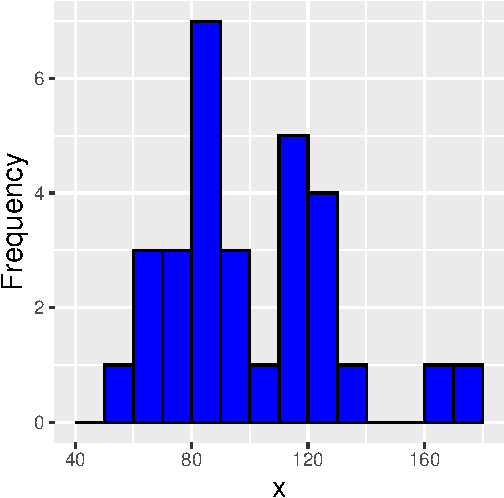
\includegraphics[keepaspectratio]{02-normal_files/figure-latex/fig-ksex-1.pdf}}

}

\caption{\label{fig-ksex}Histogram of a dataset with sample size
\(n = 30\). Is it plausible that these data are normally distributed?}

\end{figure}%

\begin{quote}
The sample statistics for these data are \(\bar{X} = 100.6\) and
\(S = 29.8\). In Figure~\ref{fig-ksecdf}, we plot the empirical cdf for
these data, overlaying the cdf for a \(\mathcal{N}(100.6,29.8^2)\)
distribution.
\end{quote}

\begin{verbatim}
Warning: Removed 1 row containing missing values or values outside the scale range
(`geom_segment()`).
\end{verbatim}

\begin{figure}

\centering{

\pandocbounded{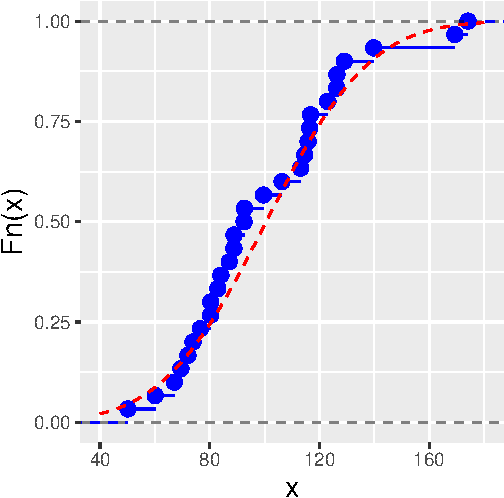
\includegraphics[keepaspectratio]{02-normal_files/figure-latex/fig-ksecdf-1.pdf}}

}

\caption{\label{fig-ksecdf}Empirical cumulative distribution function of
our dataset with the cdf for a \(\mathcal{N}(100.6,29.8^2)\)
distribution overlaid as the red dashed line.}

\end{figure}%

\begin{quote}
The largest difference between the empirical cdf and the overlaid normal
cdf in Figure~\ref{fig-ksecdf} occurs at \(x \approx 93\). Is this
difference large enough for us to decide the data are not normally
distributed with the inferred parameters \(\mu = 100.6\) and
\(\sigma = 29.8\)?
\end{quote}

\begin{Shaded}
\begin{Highlighting}[]
\FunctionTok{ks.test}\NormalTok{(x, }\StringTok{"pnorm"}\NormalTok{, }\FloatTok{100.6}\NormalTok{, }\FloatTok{29.8}\NormalTok{)}
\end{Highlighting}
\end{Shaded}

\begin{verbatim}

    Exact one-sample Kolmogorov-Smirnov test

data:  x
D = 0.13858, p-value = 0.5649
alternative hypothesis: two-sided
\end{verbatim}

\begin{quote}
By default, \texttt{ks.test()} performs a two-sided test; type
\texttt{?ks.test} in the \texttt{R} console to see how to specify
alternatives. According to this test, the \(p\)-value is 0.56. We
formally introduce \(p\)-values below, in the next section; it suffices
to say here that if \(p < \alpha\), where \(\alpha\) is the
user-specified Type I error (typically 0.05), we reject the null, so
here we fail to reject the null hypothesis that the data are normally
distributed. In truth, the simulated data are sampled from a gamma
distribution (see Section~\ref{sec-chap4gamma}); with a larger sample
size, the test becomes more better able to differentiate between
normally distributed and gamma-distributed data, so eventually we
\emph{would} reject the null hypothesis.
\end{quote}

\subsubsection{The Shapiro-Wilk Test}\label{the-shapiro-wilk-test}

\begin{quote}
The Shapiro-Wilk test has the null hypothesis that our \(n\) iid data
are sampled according to a normal distribution. The test statistic
\(Y\), which utilizes order statistics (a concept we introduce in
Section~\ref{sec-chap3order}), is complicated and will not be reproduced
here. It suffices for now for us to make three points.
\end{quote}

\begin{quote}
\begin{itemize}
\tightlist
\item
  The Shapiro-Wilk test is a more powerful test than the KS test. (This
  makes sense because the SW test is built to be more
  ``specific''\(-\)it is just used to test for normality). In other
  words, given the same data, the SW test will almost always output a
  smaller \(p\)-value than the KS test. See Figure~\ref{fig-distp}.
\end{itemize}
\end{quote}

\begin{quote}
\begin{itemize}
\tightlist
\item
  The sampling distribution for \(Y\) is non-analytic and thus the
  rejection region is estimated numerically, and thus the Shapiro-Wilk
  test cannot be used in \texttt{R} with samples of size \(>\) 5000. If
  our sample size is larger, we should randomly sub-sample the data
  before performing the SW test.
\end{itemize}
\end{quote}

\begin{quote}
\begin{itemize}
\tightlist
\item
  The Shapiro-Wilk test will often reject the null hypothesis of
  normality even when the data appear by eye to be very nearly normally
  distributed. This goes back to one of the points made above: we still
  might be able to glean ``useful'' results when performing normal-based
  hypothesis tests using technically non-normal data. Tread carefully,
  and simulate if necessary.
\end{itemize}
\end{quote}

\begin{quote}
Below, we demonstrate the use of the Shapiro-Wilk test with the
gamma-distributed data of the first example above.
\end{quote}

\begin{Shaded}
\begin{Highlighting}[]
\FunctionTok{shapiro.test}\NormalTok{(x)}
\end{Highlighting}
\end{Shaded}

\begin{verbatim}

    Shapiro-Wilk normality test

data:  x
W = 0.9508, p-value = 0.1776
\end{verbatim}

\begin{quote}
We see that while the KS test returned a \(p\)-value of 0.56, the
Shapiro-Wilk test returns the value 0.18. This value is still larger
than \(\alpha = 0.05\), so we still fail to reject the null.
\end{quote}

\begin{figure}

\begin{minipage}[t]{0.50\linewidth}

\centering{

\pandocbounded{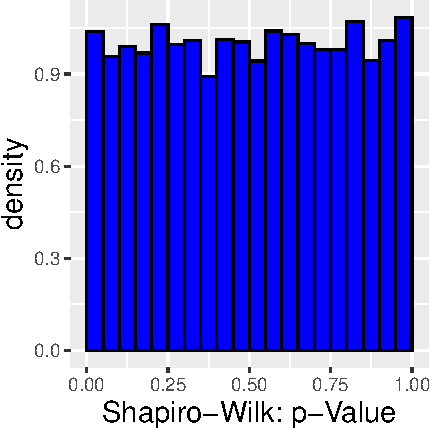
\includegraphics[keepaspectratio]{02-normal_files/figure-latex/fig-distp-1.pdf}}

}

\subcaption{\label{fig-distp-1}}

\end{minipage}%
%
\begin{minipage}[t]{0.50\linewidth}

\centering{

\pandocbounded{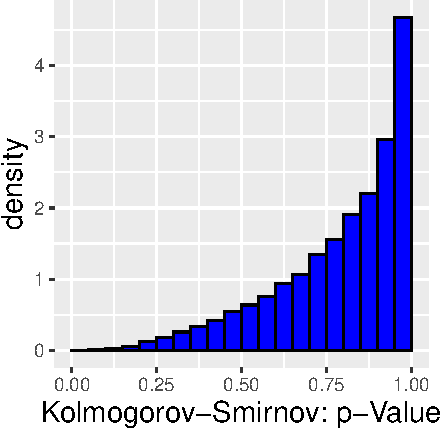
\includegraphics[keepaspectratio]{02-normal_files/figure-latex/fig-distp-2.pdf}}

}

\subcaption{\label{fig-distp-2}}

\end{minipage}%

\caption{\label{fig-distp}A comparison of \(p\)-value distributions
under the null hypothesis that we sample data from a normal
distribution, for (a) the Shapiro-Wilk test and (b) the
Kolmogorov-Smirnov test. Under the null, the distribution should be
uniform from 0 to 1: this holds for the SW test, but not for the KS
test, for which the \(p\)-values skew towards 1. This result
demonstrates that the SW test is the more powerful test for assessing
whether data are normally distributed.}

\end{figure}%

\section{Simple Linear Regression}\label{sec-chap2slr}

What to take away from this section:

\begin{itemize}
\item
  A \emph{statistical model} is a representation of the data-generating
  process.
\item
  Given a set of data tuples \(\{(x_1,Y_1),\ldots,(x_n,Y_n)\}\), where
  both the \(x_i\)'s and \(Y_i\)'s are continuously valued, we can
  attempt to determine an association between \(\mathbf{x}\) and
  \(\mathbf{Y}\) by learning a \emph{simple linear regression} model: \[
  Y_i = \beta_0 + \beta_1 x_i + \epsilon_i \,,
  \] where \(\beta_0\) and \(\beta_1\) are model coefficients and
  \(\epsilon_i\) is a random variable, the ``error term.''
\item
  For the simple linear regression model to be a valid representation of
  the data-generating process\ldots{}

  \begin{itemize}
  \item
    \(E[\epsilon_i] = 0\); and
  \item
    \(V[\epsilon_i] = \sigma^2\) for all values \(i\).
  \end{itemize}
\item
  To conduct, e.g., the hypothesis test \(H_o : \beta_1 = 0\) versus
  \(H_a : \beta_1 \neq 0\), we must add a distributional assumption; by
  convention, this assumption is that the error terms are normally
  distributed.
\end{itemize}

Thus far in this chapter, we have assumed that we have been given a
sample of iid data \(\{X_1,\ldots,X_n\} \sim
\mathcal{N}(\mu,\sigma^2)\), or, sometimes, two samples that are
independent of one another. Here we will move beyond this assumption to
the case where our data consists of tuples
\(\{(x_1,Y_1),\ldots,(x_n,Y_n)\}\) and where we want to determine (or
\emph{learn}) the association between the variables \(x_i\) and \(Y_i\).
(Assuming there is one! See Figure~\ref{fig-linreg}. Also, note the use
of the term ``association'': a relationship might exist, but it is not
necessarily the case that \(x\) ``causes'' \(Y\); to determine
causation, one would utilize methods of \emph{causal inference}, which
are beyond the scope of this book.) In other words, we want to
\emph{regress} \(\mathbf{Y}\) upon \(\mathbf{x}\).

\begin{itemize}
\tightlist
\item
  \(\mathbf{x} = \{x_1,\ldots,x_n\}\): the \emph{predictor variable} (or
  \emph{independent variable} or \emph{covariate} or \emph{feature})
\item
  \(\mathbf{Y} = \{Y_1,\ldots,Y_n\}\): the \emph{response variable} (or
  the \emph{dependent variable} or \emph{target})
\end{itemize}

\begin{figure}

\centering{

\pandocbounded{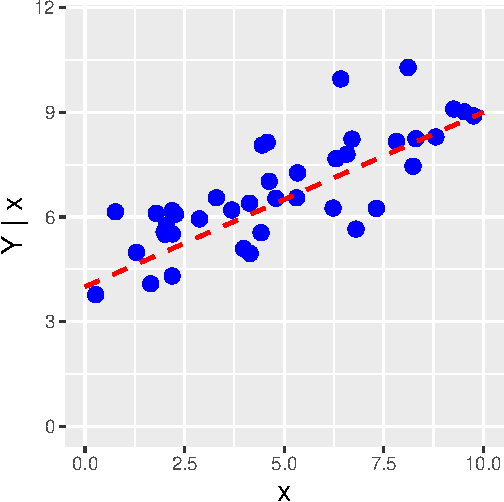
\includegraphics[keepaspectratio]{02-normal_files/figure-latex/fig-linreg-1.pdf}}

}

\caption{\label{fig-linreg}Illustration of the setting for simple linear
regression. The data \(Y \vert x\) (blue points) are randomly
distributed around the true regression line \(y \vert x = 4 + x/2\) (red
dashed line), with the error term
\(\epsilon_i \sim \mathcal{N}(y \vert 0,1)\).}

\end{figure}%

If the relationship between \(\mathbf{x}\) and \(\mathbf{Y}\) is
\emph{deterministic}, then there exists a function \(f\) such that
\(y_i = f(x_i)\) for all \(i\). As statisticians, we are more interested
in learning non-deterministic associations (so-called \emph{stochastic},
\emph{probabilistic}, or \emph{statistical} relationships) between
\(\mathbf{x}\) and \(\mathbf{Y}\). One standard model for the
data-generating process is \[
Y_i \vert x_i = f(x_i) + \epsilon_i \,,
\] where \(\{\epsilon_1,\ldots,\epsilon_n\}\) are random variables with
\(E[\epsilon_i] = 0\) and uncorrelated variances
\(V[\epsilon_i] = \sigma^2\) (i.e., the variances are the same for all
\(i\)\ldots they are \emph{homoscedastic}). (Note that we are not saying
anything about the distribution of \(\epsilon_i\) yet; we are just
stating assumptions about its expected value and variance.) Now we can
say why the predictor variable is represented in lower case while the
response variable is in upper case: we consider the predictor variable
values to be fixed, while the response variable values are random
variables because the \(\epsilon_i\)'s are random variables.

We now suppose that there is a linear relationship between
\(\mathbf{x}\) and \(\mathbf{Y}\) such that \begin{align*}
Y_i &= \beta_0 + \beta_1 x_i + \epsilon_i \\
E[Y_i] &= E[\beta_0 + \beta_1 x_i + \epsilon_i] = \beta_0 + \beta_1 x_i + E[\epsilon_i] = \beta_0 + \beta_1 x_i \\
V[Y_i] &= V[\beta_0 + \beta_1 x_i + \epsilon_i] = V[\epsilon_i] = \sigma^2 \,.
\end{align*} This is a \emph{simple linear regression} model, where the
word ``simple'' follows from the fact that there is only one predictor
variable. (Note that this is a linear model because it is linear in the
parameters; e.g., \(\beta_0 + \beta_1x_i^2\) is also a linear model.)
\(\beta_0\) is dubbed the \emph{intercept} and \(\beta_1\) is the
\emph{slope}. In analyses, we are generally interested in estimating
\(\beta_1\), as it tells us the average change in \(Y\) given a one-unit
change in \(x\).

Once a simple linear regression model is learned, we can make
predictions \[
\hat{Y}_i = \hat{\beta}_0 + \hat{\beta}_1 x_i 
\] and we can compute \emph{residuals} \[
e_i = Y_i - \hat{Y}_i
\] The goal in the estimation process is to make the residuals as small
as possible. Since negative values of \(e_i\) are as ``bad'' as positive
values, we estimate \(\beta_0\) and \(\beta_1\) by minimizing the
\emph{sum of squared errors} or \emph{SSE}: \(\sum_{i=1}^n e_i^2\).
(Note that this term is often used interchangeably with the term
\emph{residual sum of squares}, or \emph{RSS}.) This is the so-called
\emph{ordinary least squares} estimator, or OLS. Our use of the OLS
estimator for \(\beta_0\) and \(\beta_1\) (as opposed to, e.g.,
\(\sum_{i=1}^n \vert e_i \vert\)) is motivated by the \emph{Gauss-Markov
theorem}, which states that the unbiased OLS estimator is the best
estimator if the \(\epsilon_i\)'s are uncorrelated, have equal
variances, and expected values of zero (hence motivating the assumptions
stated above). Note that we have still not said anything about the
distribution of the \(\epsilon_i\)'s: the Gauss-Markov theorem does not
mandate that they have a particular distribution!

(As an aside: what happens if, e.g., we have data for which the
variances are unequal, or \emph{heteroscedastic}? We lose the ability to
make statements like ``the OLS estimator is the best linear unbiased
estimator.'' We can always learn the simple linear model we define
above\ldots a computer cannot stop us from doing so. It just may not be
the best model choice\ldots for instance, \emph{weighted OLS
regression}, where the weighting given each datum is related to how
uncertain its value is, may provide better estimates.)

To estimate \(\beta_0\) and \(\beta_1\), we take partial derivatives of
\[
\sum_{i=1}^n (Y_i - \hat{\beta}_0 - \hat{\beta}_1 x_i)^2
\] with respect to \(\hat{\beta}_0\) and \(\hat{\beta}_1\), set the
results to zero, and solve for \(\hat{\beta}_0\) and \(\hat{\beta}_1\).
Here, we will quote results, and provide the estimate of \(\sigma^2\),
while leaving the derivations as exercises to the reader:

{\def\LTcaptype{none} % do not increment counter
\begin{longtable}[]{@{}
  >{\centering\arraybackslash}p{(\linewidth - 6\tabcolsep) * \real{0.1714}}
  >{\centering\arraybackslash}p{(\linewidth - 6\tabcolsep) * \real{0.3429}}
  >{\centering\arraybackslash}p{(\linewidth - 6\tabcolsep) * \real{0.1714}}
  >{\centering\arraybackslash}p{(\linewidth - 6\tabcolsep) * \real{0.3143}}@{}}
\toprule\noalign{}
\begin{minipage}[b]{\linewidth}\centering
Parameter
\end{minipage} & \begin{minipage}[b]{\linewidth}\centering
Estimate
\end{minipage} & \begin{minipage}[b]{\linewidth}\centering
Expected Value
\end{minipage} & \begin{minipage}[b]{\linewidth}\centering
Variance
\end{minipage} \\
\midrule\noalign{}
\endhead
\bottomrule\noalign{}
\endlastfoot
\(\beta_0\) & \(\bar{Y}-\hat{\beta}_1\bar{x}\) & \(\beta_0\) &
\(\sigma^2\left(\frac{1}{n}+\frac{\bar{x}^2}{S_{xx}}\right)\) \\
\(\beta_1\) & \(\frac{S_{xY}}{S_{xx}}\) & \(\beta_1\) &
\(\frac{\sigma^2}{S_{xx}}\) \\
\(\sigma^2\) & \(\frac{1}{n-2}\) \(\sum_{i=1}^n\) \(e_i^2\)
\(=\frac{SSE}{n-2}\) & \(\sigma^2\) & \(\frac{2\sigma^4}{n-2}\) \\
\end{longtable}
}

The quantities \(S_{xx}\) and \(S_{xY}\) (and \(S_{YY}\)) are shorthand
for the following: \begin{align*}
S_{xx} &= \sum_{i=1}^n (x_i-\bar{x})^2 = \left(\sum_{i=1}^n x_i^2\right) - n\bar{x}^2 \\
S_{xY} &= \sum_{i=1}^n (x_i-\bar{x})(Y_i-\bar{Y}) = \left(\sum_{i=1}^n x_iY_i\right) - n\bar{x}\bar{Y} \\
S_{YY} &= \sum_{i=1}^n (Y_i-\bar{Y})^2 = \left(\sum_{i=1}^n Y_i^2\right) - n\bar{Y}^2 \,.
\end{align*}

In Figure~\ref{fig-linregest}, we display the estimated regression line
for the data shown above in Figure~\ref{fig-linreg}.

\begin{figure}

\centering{

\pandocbounded{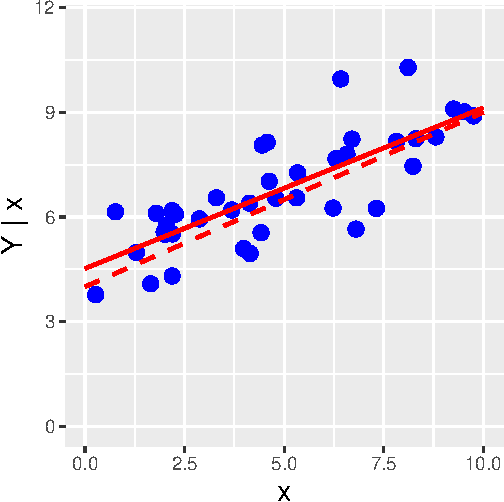
\includegraphics[keepaspectratio]{02-normal_files/figure-latex/fig-linregest-1.pdf}}

}

\caption{\label{fig-linregest}Same as the previous figure, with the
estimated regression line \(\hat{y} = 4.52 + 0.46 x\) overlaid (solid
red line).}

\end{figure}%

Ultimately, we are interested in determining if there is a statistically
significant relationship between \(\mathbf{x}\) and \(\mathbf{Y}\), a
question that we can answer using a hypothesis test: \begin{align*}
H_o&: \beta_1 = 0  \implies Y_i = \beta_0 + \epsilon_i \\
H_a&: \beta_1 \neq 0 \implies Y_i = \beta_0 + \beta_1 x_i + \epsilon_i
\end{align*} In order to carry out hypothesis testing, however, we have
to now make a distributional assumption regarding the \(\epsilon_i\)'s.
The standard assumption is that \[
\epsilon_i \sim \mathcal{N}(0,\sigma^2) \,,
\] which means that \[
Y_i \vert x_i \sim \mathcal{N}(\beta_0+\beta_1x_i,\sigma^2)
\] Adding this assumption to the model does not affect estimation; if,
for instance, we were to derive the MLE estimators for \(\beta_0\) and
\(\beta_1\), we would find that they are identical to the OLS estimators
given above.

Does our distributional assumption for the \(\epsilon_i\)'s allow us to
specify the distribution of, e.g., \(\hat{\beta}_1\)? The answer is yes.
We begin by showing that \(\hat{\beta}_1\) can be written as a linear
function of the response variable values: \begin{align*}
\hat{\beta}_1 &= \frac{\left(\sum_{i=1}^n Y_i x_i\right) - n \bar{x}\bar{Y}}{\left(\sum_{i=1}^n x_i^2\right) - n\bar{x}^2} \\
              &= \frac{1}{k} \left[ \left(\sum_{i=1}^n Y_i x_i\right) - n \bar{x}\bar{Y} \right] \\
              &= \frac{1}{k} \left[ \left(\sum_{i=1}^n Y_i x_i\right) - \sum_{i=1}^n \bar{x} Y_i \right] \\
              &= \frac{1}{k} \sum_{i=1}^n (x_i - \bar{x}) Y_i = \sum_{i=1}^n \left( \frac{x_i-\bar{x}}{k}\right) Y_i = \sum_{i=1}^n a_i Y_i \,.
\end{align*} Because the \(Y_i\)'s are normally distributed, we know
(via the method of moment-generating functions) that \(\hat{\beta}_1\)
is also normally distributed, with mean \[
E[\hat{\beta}_1] = \sum_{i=1}^n a_i E[Y_i] = \cdots = \beta_1
\] and variance \[
V[\hat{\beta}_1] = \sum_{i=1}^n a_i^2 V[Y_i] = \sum_{i=1}^n a_i^2 \sigma^2 = \cdots = \frac{\sigma^2}{\left(\sum_{i=1}^n x_i^2\right) - n\bar{x}^2} \,.
\] We can finally perform the hypothesis test. If \(\sigma^2\) is
unknown, the standardized slope is assumed to be \(t\)-distributed for
\(n-2\) degrees of freedom: \[
\frac{\hat{\beta}_1 - \beta_1}{se({\hat{\beta}_1})} = \frac{\hat{\beta}_1 - \beta_1}{\sqrt{V[{\hat{\beta}_1}]}} \sim t_{n-2} \,.
\]

To reiterate:

\begin{enumerate}
\def\labelenumi{\arabic{enumi}.}
\tightlist
\item
  The assumption that \(\epsilon_i \sim \mathcal{N}(0,\sigma^2)\) allows
  us to test hypotheses about, e.g., \(\beta_1\). If this assumption is
  violated, then OLS regression is still the best linear unbiased
  estimator.
\item
  If, in addition, the assumption that \(\epsilon_i\)'s are
  homoscedastic and uncorrelated is violated, the OLS regression will no
  longer be the best linear unbiased estimator, and we would need to
  seek alternatives, such as weighted OLS regression.
\item
  Last\ldots if, in addition, the assumption of \(E[\epsilon_i] = 0\) is
  violated, then using OLS will be a biased estimator. At this point, we
  would generally conclude that there is a better, nonlinear
  representation of the data-generating process that we should use.
\end{enumerate}

\subsection{Examples}\label{examples-24}

\subsubsection{Correlation: the Strength of Linear
Association}\label{correlation-the-strength-of-linear-association}

\begin{quote}
We can measure the strength of a linear association via the metric of
\emph{correlation}. We define the correlation between a pair of random
variables \(X\) and \(Y\) as \[
\rho_{XY} = \frac{E[XY] - E[X]E[Y]}{\sqrt{V[X]V[Y]}}\,,
\] with \(\vert \rho_{XY} \vert \leq 1\). (We will discuss correlation
and the related concept of covariance more in depth in
Section~\ref{sec-chap6covariance}. For now, just treat the equation
above as a definition. The main thing to keep in mind is that if \(X\)
and \(Y\) are independent random variables, \(\rho_{XY} = 0\), while if
\(X = Y\) or \(X = -Y\), \(\rho_{XY} = 1\) and \(-1\) respectively.) If
instead of a pair of random variables we have a set of tuples, we can
still define a correlation, which we can estimate using the
\emph{Pearson correlation coefficient}: \[
R = \frac{\sum_{i=1}^n (x_i-\bar{x})(Y_i-\bar{Y})}{\left[\sum_{i=1}^n (x_i-\bar{x})^2\right]\left[\sum_{i=1}^n (Y_i-\bar{Y})^2\right]} = \frac{S_{xY}}{\sqrt{S_{xx}S_{YY}}} = \hat{\beta}_1 \sqrt{\frac{S_{xx}}{S_{YY}}} \,.
\] The last equality follows from the fact that
\(\hat{\beta}_1 = S_{xY}/S_{xx}\). It follows from this expression that
\(R\) and \(\hat{\beta}_1\) have the same sign.
\end{quote}

\begin{quote}
Related to the correlation is the \emph{coefficient of determination},
or \(R^2\), a quantity ranging from 0 to 1 that is interpreted as the
proportion of the variation in the response variable values explained by
the predictor variable values. The closer \(R^2\) is to 1, the more
strictly linear is the association between \(x\) and \(Y\).
\end{quote}

\begin{quote}
For completeness, we mention ``adjusted \(R^2\),'' as this is an
oft-quoted output from \texttt{R}'s linear model function,
\texttt{lm()}. (See below for example usage of \texttt{lm()}.) Adjusted
\(R^2\) attempts to correct for the tendency of \(R^2\) to
over-optimistically indicate the quality of fit of a linear model. There
are several formulae for computing adjusted \(R^2\); \texttt{R} uses
Wherry's formula: \[
\mbox{Adj.}~R^2 = 1 - (1-R^2)\frac{n-1}{n-p-1} \,,
\] where \(p\) is the number of predictor variables (with \(p = 1\) for
simple linear regression).
\end{quote}

\subsubsection{The Expected Value of the Sum of Squared Errors
(SSE)}\label{the-expected-value-of-the-sum-of-squared-errors-sse}

\begin{quote}
Here we show that \(SSE/(n-2)\) is an unbiased estimator of
\(\sigma^2\). This is a non-trivial algebraic exercise, and thus we will
leave the calculation of \(V[\hat{\sigma^2}] = V[SSE/(n-2)] =
2\sigma^4/(n-2)\) as an exercise to the (masochistic) reader.
\end{quote}

\begin{quote}
We start by writing that \begin{align*}
SSE = \sum_{i=1}^n e_i^2 &= \sum_{i=1}^n (Y_i - \hat{Y}_i)^2 \\
&= \sum_{i=1}^n [Y_i - (\hat{\beta}_0 + \hat{\beta}_1 x_i)]^2 \\
&= \sum_{i=1}^n [Y_i - (\bar{Y} - \hat{\beta}_1 \bar{x} + \hat{\beta}_1 x_i)]^2 \\
&= \sum_{i=1}^n [(Y_i - \bar{Y}) - \hat{\beta}_1 (x_i-\bar{x})]^2 \\
&= \sum_{i=1}^n [(Y_i - \bar{Y})^2 - 2 \hat{\beta}_1 (x_i-\bar{x})(Y_i - \bar{Y}) + \hat{\beta}_1^2(x_i-\bar{x})^2] \\
&= S_{YY} - 2 \hat{\beta}_1 S_{xY} + \hat{\beta}_1^2 S_{xx} \\
&= S_{YY} - 2 \hat{\beta}_1 (S_{xx} \hat{\beta}_1) + \hat{\beta}_1^2 S_{xx} \\
&= S_{YY} - \hat{\beta}_1^2 S_{xx} \,.
\end{align*} To find the expected value of this difference, we look
first at \(S_{YY}\) and then at \(\hat{\beta}_1^2 S_{xx}\).
\begin{align*}
E[S_{YY}] &= E\left[ \sum_{i=1}^n (Y_i - \bar{Y})^2 \right] \\
&= E\left[ \sum_{i=1}^n \left(\beta_0 + \beta_1x_i + \epsilon_i - \beta_0 - \beta_1 \bar{x} - \bar{\epsilon} \right)^2 \right] \\
&= E\left[ \sum_{i=1}^n \left(\beta_1(x_i -\bar{x}) + (\epsilon_i - \bar{\epsilon}) \right)^2 \right] \\
&= E\left[ \sum_{i=1}^n \beta_1^2(x_i -\bar{x})^2 + \sum_{i=1}^n 2 \beta_1 (x_i - \bar{x})(\epsilon_i - \bar{\epsilon}) + \sum_{i=1}^n (\epsilon_i - \bar{\epsilon})^2 \right] \\
&= E\left[ \beta_1^2 S_{xx} + 2 \beta_1 \sum_{i=1}^n (x_i - \bar{x})(\epsilon_i - \bar{\epsilon}) + \sum_{i=1}^n (\epsilon_i - \bar{\epsilon})^2 \right] \\
&= \beta_1^2 S_{xx} + 2 \beta_1 \sum_{i=1}^n (x_i - \bar{x}) E\left[ \epsilon_i - \bar{\epsilon} \right] + \sum_{i=1}^n E\left[ (\epsilon_i - \bar{\epsilon})^2 \right] \,.
\end{align*} Since \(E[\epsilon_i] = E[\bar{\epsilon}] = 0\), the middle
term vanishes. As for the right-most term: \begin{align*}
\sum_{i=1}^n E\left[ (\epsilon_i - \bar{\epsilon})^2 \right] &= \sum_{i=1}^n E\left[ \epsilon_i^2 - 2\epsilon_i \bar{\epsilon} + \bar{\epsilon}^2 \right] \\
&= \sum_{i=1}^n E\left[ \epsilon_i^2 \right] - 2 \sum_{i=1}^n E\left[\epsilon_i \bar{\epsilon}\right] + \sum_{i=1}^n E\left[\bar{\epsilon}^2\right] \\
&= \sum_{i=1}^n E\left[ \epsilon_i^2 \right] - 2 E\left[ \bar{\epsilon} \sum_{i=1}^n \epsilon_i \right] + E\left[ \sum_{i=1}^n \bar{\epsilon}^2\right] \\
&= \sum_{i=1}^n V[\epsilon_i] + \sum_{i=1}^n \left(E[\epsilon_i]\right)^2 - 2 n E\left[ \bar{\epsilon}^2 \right] + n E\left[ \bar{\epsilon}^2\right] \\
&= \sum_{i=1}^n \sigma^2 - n E\left[ \bar{\epsilon}^2 \right] \\
&= n \sigma^2 - n \frac{\sigma^2}{n} = (n-1)\sigma^2 \,.
\end{align*} So at this point, we have that \[
E[S_{YY}] = S_{xx} \beta_1^2 + (n-1)\sigma^2 \,.
\] Now let's look at \(E[\hat{\beta}_1^2 S_{xx}]\): \begin{align*}
E\left[\hat{\beta}_1^2 S_{xx}\right] &= S_{xx} E\left[\hat{\beta}_1^2\right] \\
&= S_{xx} \left( V\left[ \hat{\beta}_1 \right] + \left( E\left[ \hat{\beta}_1 \right] \right)^2 \right) \\
&= S_{xx} \left( \frac{\sigma^2}{S_{xx}} + \beta_1^2 \right) \\
&= \sigma^2 + S_{xx} \beta_1^2 \,.
\end{align*} So \[
E[SSE] = S_{xx} \beta_1^2 + (n-1)\sigma^2 - \sigma^2 - S_{xx} \beta_1^2 = (n-2)\sigma^2 \,.
\] Thus \(SSE/(n-2)\) is an unbiased estimator of \(\sigma^2\).
\end{quote}

\subsubsection{Linear Regression in R}\label{linear-regression-in-r}

\begin{quote}
Below, we show the results of learning a linear regression model using
\texttt{R}. The data are the same as used to produce
Figure~\ref{fig-linregest}, with the parameter estimates output by
\texttt{lm()} mapping directly to the solid red line in that figure.
\end{quote}

\begin{Shaded}
\begin{Highlighting}[]
\CommentTok{\# lm(): "linear model"}
\CommentTok{\# y\textasciitilde{}x : this is a "model formula" that in words translates as}
\CommentTok{\#       "regress the response data y upon the predictor data x"}
\CommentTok{\#       or "estimate beta\_0 and beta\_1 for the model E[Y] = beta\_0 + beta\_1 x"}
\NormalTok{lm.out }\OtherTok{=} \FunctionTok{lm}\NormalTok{(y }\SpecialCharTok{\textasciitilde{}}\NormalTok{ x)}

\CommentTok{\# show a summary of the model}
\FunctionTok{summary}\NormalTok{(lm.out)}
\end{Highlighting}
\end{Shaded}

\begin{verbatim}

Call:
lm(formula = y ~ x)

Residuals:
     Min       1Q   Median       3Q      Max 
-2.00437 -0.53068  0.04523  0.40338  2.47660 

Coefficients:
            Estimate Std. Error t value Pr(>|t|)    
(Intercept)   4.5231     0.3216  14.063  < 2e-16 ***
x             0.4605     0.0586   7.859 1.75e-09 ***
---
Signif. codes:  0 '***' 0.001 '**' 0.01 '*' 0.05 '.' 0.1 ' ' 1

Residual standard error: 0.9792 on 38 degrees of freedom
Multiple R-squared:  0.6191,    Adjusted R-squared:  0.609 
F-statistic: 61.76 on 1 and 38 DF,  p-value: 1.749e-09
\end{verbatim}

\begin{quote}
\begin{enumerate}
\def\labelenumi{\arabic{enumi}.}
\tightlist
\item
  The model residuals \(Y_i - \hat{Y}_i\) are summarized via five
  numbers (minimum, maximum, and median, along with the
  25\(^{\mathrm{th}}\) and 75\(^{\mathrm{th}}\) percentile values). If,
  e.g., the median is substantially different from zero, it is possible
  that the assumption that \(Y \vert x\) is normally distributed is
  violated\ldots and it is possible that the assumption
  \(E[\epsilon_i] = 0\) is violated as well.
\item
  Under \texttt{Coefficients}, there are four numerical columns. The
  first shows \(\hat{\beta}_0\) (\texttt{(Intercept)}) and
  \(\hat{\beta}_1\) (\texttt{x}), the second shows the estimated
  standard errors for these statistics, the third is simply the ratio of
  the values in the first and second columns, and the fourth is the
  \(p\)-value. The third and fourth columns are distribution-specific:
  the hypothesis test being carried out has a null of zero, and the
  \texttt{t\ value} is assumed to be \(t\)-distributed for \(n-2\)
  degrees of freedom. The \(p\)-values in the fourth column are
  \(\ll \alpha = 0.05\), which lead us to decide that both the intercept
  and the slope are truly non-zero. (In our simulation, they are:
  \(\beta_0 = 4\) and \(\beta_1 = 0.5\).)
\item
  The \texttt{Residual\ standard\ error} shows the value of
  \(\hat{\sigma} = \sqrt{SSE/(n-2)}\), while the ``38 degrees of
  freedom'' indicates that \(n = 40\). We note that in this simulation,
  \(\sigma^2 = 1\).
\item
  The meanings behind the \texttt{R-squared} values are explained above
  in the correlation example. In words, approximately 60\% of the
  variation exhibited by the data is accounted for with the linear
  model.
\item
  Last, the line with the phrase \texttt{F-statistic} shows the result
  of a hypothesis test in which (in general) the null is that all the
  \(\beta_i\)'s (excluding \(\beta_0\)) are zero and the alternative is
  that at least one of the \(\beta_i\)'s is non-zero. Here, since there
  is only one non-intercept coefficient, the \(p\)-value is equivalent
  to the one printed under \texttt{Coefficients}. We will discuss where
  the \texttt{F-statistic} and \texttt{DF} numbers come from below in
  the next section.
\end{enumerate}
\end{quote}

\section{One-Way Analysis of Variance}\label{sec-chap2anova}

What to take away from this section:

\begin{itemize}
\tightlist
\item
  Given a set of data tuples \(\{(x_1,Y_1),\ldots,(x_n,Y_n)\}\), where
  the \(x_i\)'s are discretely valued (and perhaps categorical, with no
  explicit ordering) and where the \(Y_i\)'s are normally distributed
  random variables, we can use \emph{one-way analysis of variance} to
  test the hypothesis that the sample means of \(Y\) given each value of
  \(x\) are the same.
\end{itemize}

In the simple linear regression setting, our data consists of a
continuously distributed predictor variable \(\mathbf{x}\) and response
variable \(\mathbf{Y}\). What if, instead, the predictor variable values
come in \emph{groups}? For instance, we might wish to determine the time
a person needs to accomplish a task after eating either chocolate or
vanilla ice cream. To do this, we might map the eating of chocolate to a
particular value of \(x\), say \(x = 0\), and the eating of vanilla to
another value of \(x\), say \(x = 1\). Then, if we continue to adopt a
simple linear regression framework, we have that \begin{align*}
Y_i &= \beta_0 + \beta_1 x_i + \epsilon_i \\
E[Y_i \vert x_i = 0] &= \beta_0 \\
E[Y_i \vert x_i = 1] &= \beta_0 + \beta_1 \,.
\end{align*} To see if there is a difference in task-accomplishment time
between groups, we would test the hypothesis \(H_o: \beta_1 = 0\) versus
\(H_a: \beta_1 \neq 0\). As the value of the slope is meaningless,
beyond whether or not it is zero (because the mapping from group
characteristics to values of \(x\) is arbitrary), we would not run a
conventional linear regression analysis; rather, if we assume that
\(\bar{Y} \vert x_i\) is normally distributed, we would run a two-sample
\(t\) test like the Welch's \(t\) test described in an example in
Section~\ref{sec-chap2hypothesis} to determine whether
\(\bar{Y} \vert x_i=0\) is drawn from a distribution with the same
population mean as \(\bar{Y} \vert x_i=1\).

What if there are more than two groups (or \emph{treatments})? For
instance, what if we redo the experiment but add strawberry ice cream?
When the number of groups is greater than two, we move from the
two-sample \(t\) test to \emph{one-way analysis of variance} (or one-way
\emph{ANOVA}; the ``one-way'' indicates that there is a single predictor
variable, which in our example is ice cream flavor). See
Figure~\ref{fig-anova}.

\begin{figure}

\begin{minipage}[t]{0.50\linewidth}

\centering{

\pandocbounded{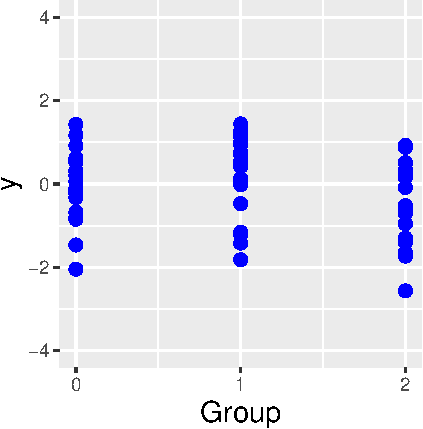
\includegraphics[keepaspectratio]{02-normal_files/figure-latex/fig-anova-1.pdf}}

}

\subcaption{\label{fig-anova-1}}

\end{minipage}%
%
\begin{minipage}[t]{0.50\linewidth}

\centering{

\pandocbounded{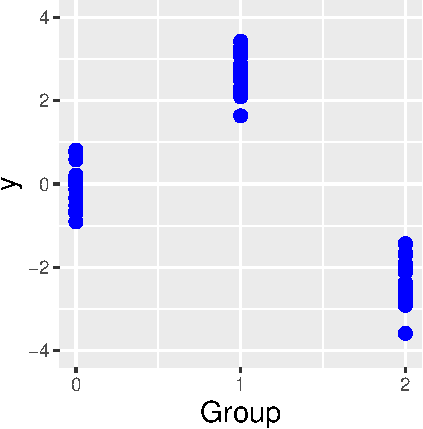
\includegraphics[keepaspectratio]{02-normal_files/figure-latex/fig-anova-2.pdf}}

}

\subcaption{\label{fig-anova-2}}

\end{minipage}%

\caption{\label{fig-anova}Illustration of the setting for a one-way
analysis of variance. In (a), the spread of the data within each group
is large compared to the differences in means between each group, so an
ANOVA is less likely to reject the null hypothesis that
\(\mu_0 = \mu_1 = \mu_2\). In (b), the spread of data within groups is
small relative to the differences in means between groups, so an ANOVA
is more likely to reject the null hypothesis.}

\end{figure}%

Let the index \(i\) denote a particular group (chocolate ice-cream
eaters, etc.) and let the index \(j\) denote different data within the
same group. Let \(n_i\) denote the sample size within each group, and
let \(k\) denote the total number of groups. The total sum of squares is
defined as the sum of squared differences between \(Y_i\) and
\(\bar{Y}\), which in this setting can be expressed via a double
summation, one over data within a group, and another over groups:
\begin{align*}
\mbox{Total SS} &= \sum_{i=1}^k \sum_{j=1}^{n_i} (Y_{ij} - \bar{Y})^2 = \sum_{i=1}^k \sum_{j=1}^{n_i} (Y_{ij}-\bar{Y}_{i\bullet})^2 + \sum_{i=1}^k n_i(\bar{Y}_{i\bullet}-\bar{Y})^2\\
&= SSE + SST \,,
\end{align*} where \(\bar{Y}_{i\bullet}\) is the average value for group
\(i\), \(SSE\) has its usual meaning as the sum of squared errors
(although here \(\hat{\beta}_0+\hat{\beta}_1x_i\) is replaced with the
estimated group mean \(\bar{Y}_{i\bullet}\)), and \(SST\) is the sum of
squared average treatment effects. If the \(SSE\) value is large
relative to the \(SST\) value, then we are in a situation where the data
are spread widely within each group relative to the spread in values of
the group means. In such a situation, it would be difficult to detect a
statistically significant difference between the group means. (See the
left panel of Figure~\ref{fig-anova}.) On the other hand, if the \(SST\)
value is large relative to the \(SSE\) value, then the group means have
a wide spread compared to the data in each group. In such a situation,
it would be much easier to detect a statistically significant difference
between the group means. (See the right panel of
Figure~\ref{fig-anova}.) This reasoning motivates using the ratio of
\(SST\) to \(SSE\) as the hypothesis test statistic. However, we do not
know its distribution\ldots or at least, not yet. We do know is that
under the null, \begin{align*}
W_T = \frac{SST}{\sigma^2} &\sim \chi_{k-1}^2 \\
W_E = \frac{SSE}{\sigma^2} &\sim \chi_{n-k}^2 \,.
\end{align*} And we know that \[
F = \frac{W_1/\nu_1}{W_2/\nu_2} \sim F_{\nu_1,\nu_2} \,,
\] i.e., the ratio of chi-square distributed random variables, each
divided by their respective number of degrees of freedom, is
\(F\)-distributed for \(\nu_1\) numerator and \(\nu_2\) denominator
degrees of freedom. Thus \[
F = \frac{SST/(k-1)}{SSE/(n-k)} = \frac{MST}{MSE} \sim F_{k-1,n-k} \,.
\] In the ANOVA hypothesis test, the null hypothesis \(H_o\) is that
\(E[Y_1] = E[Y_2] = \cdots = E[Y_k]\), and the alternative hypothesis is
that at least one mean is different from the others. If we test at level
\(\alpha\), we reject the null hypothesis if
\(F > F_{1-\alpha,k-1,n-k}\). In \texttt{R}, the boundary of the
rejection region would be given by
\texttt{qf(1\ -\ alpha,\ k\ -\ 1,\ n\ -\ k)} while the \(p\)-value would
be given by \texttt{1\ -\ pf(F.obs,\ k\ -\ 1,\ n\ -\ k)}.

\subsection{Examples}\label{examples-25}

\subsubsection{One-Way ANOVA: the Statistical
Model}\label{one-way-anova-the-statistical-model}

\begin{quote}
In the notes above, we build up the test statistic for the one-way
ANOVA, but we do not discuss the underlying statistical model. We can
write down the model as \[
Y_{ij} = \mu + \tau_i + \epsilon_{ij} \,,
\] where \(i\) denotes the treatment group and \(j\) denotes an observed
datum within group \(i\). \(\mu\) is the overall mean response, while
\(\tau_i\) is the \emph{deterministic} effect of treatment in group
\(i\). (\(\tau\) is the Greek letter tau, which is pronounced ``tao''
{[}rhyming with ``ow,'' an expression of pain{]}. Recall that by
``deterministic'' we mean that \(\tau_i\) is \emph{not random}.) The
error terms \(\epsilon_{ij}\) are independent, normally distributed, and
homoscedastic with variance \(\sigma^2\).
\end{quote}

\begin{quote}
Recall that \(\bar{Y}_{i\bullet}\) is the sample mean within group
\(i\). We know it is distributed normally (by assumption) but what are
its expected value and variance?
\end{quote}

\begin{quote}
The expected value is \begin{align*}
E[\bar{Y}_{i\bullet}] &= E\left[\frac{1}{n_i}\sum_{j=1}^{n_i} Y_{ij}\right] = \frac{1}{n_i}\sum_{j=1}^{n_i} E[Y_{ij}] \\
&= \frac{1}{n_i}\sum_{j=1}^{n_i} E[\mu + \tau_i + \epsilon_{ij}] = \mu + \tau_i + E[\epsilon_{ij}] = \mu+\tau_i \,,
\end{align*} while the variance is \begin{align*}
V[\bar{Y}_{i\bullet}] &= V\left[\frac{1}{n_i}\sum_{j=1}^{n_i} Y_{ij}\right] = \frac{1}{n_i}\sum_{j=1}^{n_i^2} V[Y_{ij}] = \frac{1}{n_i^2}\sum_{j=1}^{n_i} V[\mu + \tau_i + \epsilon_{ij}]\\
&= \frac{n_i V[\epsilon_{ij}]}{n_i^2} = \frac{\sigma^2}{n_i} \,.
\end{align*} Thus
\(\bar{Y}_{i\bullet} \sim \mathcal{N}(\mu+\tau_i,\sigma^2/n_i)\).
\end{quote}

\subsubsection{Linear Regression in R:
Redux}\label{linear-regression-in-r-redux}

\begin{quote}
The last example of the last section showed the output from
\texttt{lm()}, \texttt{R}'s linear model function:
\end{quote}

\begin{Shaded}
\begin{Highlighting}[]
\FunctionTok{summary}\NormalTok{(lm.out)}
\end{Highlighting}
\end{Shaded}

\begin{verbatim}

Call:
lm(formula = y ~ x)

Residuals:
     Min       1Q   Median       3Q      Max 
-2.00437 -0.53068  0.04523  0.40338  2.47660 

Coefficients:
            Estimate Std. Error t value Pr(>|t|)    
(Intercept)   4.5231     0.3216  14.063  < 2e-16 ***
x             0.4605     0.0586   7.859 1.75e-09 ***
---
Signif. codes:  0 '***' 0.001 '**' 0.01 '*' 0.05 '.' 0.1 ' ' 1

Residual standard error: 0.9792 on 38 degrees of freedom
Multiple R-squared:  0.6191,    Adjusted R-squared:  0.609 
F-statistic: 61.76 on 1 and 38 DF,  p-value: 1.749e-09
\end{verbatim}

\begin{quote}
In that example, we indicated that the numbers on the line beginning
\texttt{F-statistic} would make more sense after we covered one-way
analysis of variance.
\end{quote}

\begin{quote}
There are two coefficients in this model, which is analogous to two
``treatment groups.'' Hence \(k = 2\),
\(SST/\sigma^2 \sim \chi_{k-1=1}^2\), and
\(SSE/\sigma^2 \sim \chi_{n-k=38}^2\). This explains
\texttt{on\ 1\ and\ 38\ DF}. The \(F\) statistic is \(MST/MSE = 61.76\),
which under the null is sampled according to an \(F\) distribution with
1 numerator and 38 denominator degrees of freedom. This is an extreme
value under the null, as indicated by the \(p\)-value 1.749
\(\times 10^{-9}\)\ldots so we conclude that the true value of the slope
\(\beta_1\) is not zero.
\end{quote}

\begin{quote}
But there's more. To access more information about the \(F\) test that
is carried out, we can call the \texttt{anova()} function.
\end{quote}

\begin{Shaded}
\begin{Highlighting}[]
\FunctionTok{anova}\NormalTok{(lm.out)}
\end{Highlighting}
\end{Shaded}

\begin{verbatim}
Analysis of Variance Table

Response: y
          Df Sum Sq Mean Sq F value    Pr(>F)    
x          1 59.208  59.208  61.756 1.749e-09 ***
Residuals 38 36.432   0.959                      
---
Signif. codes:  0 '***' 0.001 '**' 0.01 '*' 0.05 '.' 0.1 ' ' 1
\end{verbatim}

\begin{quote}
This function call outputs information we could not see above: the
\(SST\) (the first row of \texttt{Sum\ Sq}), \(SSE\) (second row),
\(MST\) (the first row of \texttt{Mean\ Sq}), and \(MSE\) (second row).
The \texttt{F\ value} is the ratio \(MST/MSE\); here, that is
59.208/0.959 = 61.756.
\end{quote}

\section{The Exponential Family of
Distributions}\label{sec-chap2exponential}

What to take away from this section:

\begin{itemize}
\item
  The normal distribution is a member of a larger set of distributions
  that is dubbed the \emph{exponential family of distributions}.
\item
  Foreshadowing: members of the exponential family have, as we will see
  in Section~\ref{sec-chap3nplemma}, single-valued \emph{sufficient
  statistics} that are the optimal statistics to use when performing
  statistical inference.
\end{itemize}

We conclude this chapter by placing the normal distribution into a
larger context: the \emph{exponential family} of distributions, which
encompasses the normal as well as, e.g., the binomial, beta, Poisson,
and gamma distributions, the ones that serve as the foci for Chapters
\hyperref[sec-chap3]{3} and \hyperref[sec-chap4]{4}. Knowing about the
exponential family and its properties will help us better understand
concepts of statistical inference that we introduce in those chapters,
such as the concept of sufficiency.

Let's assume that we are examining a distribution \(P\) that has one
freely varying parameter \(\theta\). \(P\) is a member of the
exponential family of distributions if we can express, e.g., its
probability density function as \begin{align*}
f_X(x \vert \theta) = h(x) \exp\left[\eta(\theta) T(x) - A(\theta)\right] \,.
\end{align*} (This same result holds for a mass function
\(p_X(x \vert \theta)\) as well. Note that \(\theta\) cannot be a
domain-specifying parameter, so a distribution whose domain is, e.g.,
\(x \in [0,\theta]\) cannot belong to the exponential family.)

Let's see how this works with a normal distribution of known variance:
\begin{align*}
f_X(x \vert \mu) &= \frac{1}{\sqrt{2\pi\sigma^2}} \exp\left[-\frac{1}{2\sigma^2}(x-\mu)^2\right]\\
&= \frac{1}{\sqrt{2\pi\sigma^2}} \exp\left(-\frac{x^2}{2\sigma^2}\right) \exp\left(\frac{x\mu}{\sigma^2}\right) \exp\left(-\frac{\mu^2}{2\sigma^2}\right) \,.
\end{align*} From this, we can directly read off the functions that
together comprise the exponential family form: \begin{align*}
h(x) &= \frac{1}{\sqrt{2\pi\sigma^2}} \exp\left(-\frac{x^2}{2\sigma^2}\right) \\
\eta(\mu) &= \frac{\mu}{\sigma^2} \\
T(x) &= x \\
A(\mu) &= \frac{\mu^2}{2\sigma^2} \,.
\end{align*} We note that we can also define \(\eta(\mu) = \mu\) and
\(T(x) = x/\sigma^2\). Ultimately, the choice of where to place any
constants (either within the \(\eta(\cdot)\) function or within
\(T(\cdot)\) function) makes no difference when we are performing
inferential tasks.

\subsection{Example}\label{example-4}

\subsubsection{Exponential Family with a Vector of
Parameters}\label{exponential-family-with-a-vector-of-parameters}

\begin{quote}
The more general functional form of the exponential family that we use
when a distribution has \(p \geq 2\) parameters is \begin{align*}
f_X(x \vert \boldsymbol{\theta}) = h(x) \exp\left[\left(\sum_{i=1}^p \eta_i(\boldsymbol{\theta}) T_i(x)\right) - A(\boldsymbol{\theta})\right] \,.
\end{align*} For the normal distribution with unknown mean and variance,
we can examine the expression \begin{align*}
f_X(x \vert \mu) = \frac{1}{\sqrt{2\pi\sigma^2}} \exp\left(-\frac{x^2}{2\sigma^2}\right) \exp\left(\frac{x\mu}{\sigma^2}\right) \exp\left(-\frac{\mu^2}{2\sigma^2}\right) \,,
\end{align*} and, after noting that \begin{align*}
\frac{1}{\sqrt{2\pi\sigma^2}} = \exp\left(\log\left(\frac{1}{\sqrt{2\pi\sigma^2}}\right)\right) = \exp\left(-\frac12 \log\left(2 \pi \sigma^2\right) \right) \,,
\end{align*} we can read off the constituent functions: \begin{align*}
h(x) &= 1 \\
\eta_1(\mu,\sigma^2) &= -\frac{1}{2\sigma^2} \\
T_1(x) &= x^2 \\
\eta_2(\mu,\sigma^2) &= \frac{\mu}{\sigma^2} \\
T_2(x) &= x \\
A(\mu,\sigma^2) &= \frac{\mu^2}{2\sigma^2} + \frac12 \log\left(2 \pi \sigma^2\right) \,.
\end{align*}
\end{quote}

\section{Exercises}\label{sec-chap2exercises}

\begin{enumerate}
\def\labelenumi{\arabic{enumi}.}
\item
  We are given that \(X \sim \mathcal{N}(4,4)\). (a) What is
  \(P(X > 2 \vert X > 0)\), in terms of \(\Phi(\cdot)\) and/or
  \(\Phi^{-1}(\cdot)\)? (b) Determine the value \(c\) such that
  \(P(X < c \vert X < 4) = 0.5\); leave your answer in terms of
  \(\Phi(\cdot)\) and/or \(\Phi^{-1}(\cdot)\).
\item
  What is \(E[e^{-Z^2/2}]\) if \(Z \sim \mathcal{N}(0,1)\)?
\item
  A filtering machine only passes through widgets that have masses
  between 4 and 6. Assume that the mass of a widget is a random variable
  \(M \sim \mathcal{N}(5,4)\). (a) What is the probability that the
  filtering machine will reject any given widget? Leave your answer in
  terms of \(\Phi(\cdot)\) and/or \(\Phi^{-1}(\cdot)\), both here and in
  part (b). (b) Now assume that \(\sigma\) is unknown. What is
  \(\sigma\) such that the probability of rejection is 0.02?
\item
  We are given that \(X_1\) and \(X_2\) are iid draws from a normal
  distribution with mean \(\mu\) and variance \(\sigma^2\). What is the
  value of \(c\) such that the probability of \(X_1 < \mu - c\) and
  \(X_2 > \mu\) is 1/4? Leave the answer in terms of \(\Phi(\cdot)\)
  and/or \(\Phi^{-1}(\cdot)\).
\item
  The moment-generating function for the Laplace distribution is
  \begin{align*}
  m(t) = \frac{\exp(a t)}{1 - b^2 t^2} \,.
  \end{align*} Derive \(E[X]\) for this distribution.
\item
  We are given the probability mass function shown below. (a) Derive the
  moment-generating function for this distribution. (b) Use the derived
  mgf to compute \(E[X]\).
\end{enumerate}

{\def\LTcaptype{none} % do not increment counter
\begin{longtable}[]{@{}cccc@{}}
\toprule\noalign{}
\endhead
\bottomrule\noalign{}
\endlastfoot
\(x\) & 0 & 1 & 2 \\
\(p_X(x)\) & 0.2 & 0.4 & 0.4 \\
\end{longtable}
}

\begin{enumerate}
\def\labelenumi{\arabic{enumi}.}
\setcounter{enumi}{6}
\item
  We are given the following probability density function:
  \begin{align*}
  f_X(x) = ke^{-x} \,,
  \end{align*} for \(x \in [0,a]\). \(k\) is a constant that need not be
  evaluated. (a) Write down the moment-generating function associated
  with this pdf. (b) Determine \(E[X]\) for this pdf.
\item
  We are given the two probability mass functions shown below. (a) Write
  down the moment-generating functions for both \(X_1\) and \(X_2\). (b)
  Write down the moment-generating function for the random variable
  \(Y = X_1 + 2X_2\).
\end{enumerate}

{\def\LTcaptype{none} % do not increment counter
\begin{longtable}[]{@{}cccc@{}}
\toprule\noalign{}
\endhead
\bottomrule\noalign{}
\endlastfoot
\(x_1\) & \(p_{X_1}(x_1)\) & \(x_2\) & \(p_{X_2}(x_2)\) \\
0 & 0.4 & 0 & 0.2 \\
1 & 0.6 & 1 & 0.8 \\
\end{longtable}
}

\begin{enumerate}
\def\labelenumi{\arabic{enumi}.}
\setcounter{enumi}{8}
\item
  The Rademacher distribution is \begin{align*}
  p_X(x) = \left\{ \begin{array}{cc} \frac12 & x = -1 \\ \frac12 & x = 1 \end{array} \right. \,.
  \end{align*} (a) Derive the moment-generating function for a
  Rademacher random variable. (b) Assume that we have drawn \(n\) iid
  data from the Rademacher distribution. Write down the
  moment-generating function for the sample mean,
  \(\bar{X} = (\sum_{i=1}^n X_i)/n\).
\item
  We are given the following probability density function:
  \begin{align*}
  f_X(x) = \left\{ \begin{array}{cc} 1/3 & x \in [0,1/2) \\ 2/3 & x \in [1/2,1] \end{array} \right. \,.
  \end{align*} Derive the moment-generating function for \(X\).
\item
  We sample \(n = 16\) iid data from a normal distribution with mean 5.
  The sample variance is 9. (a) Compute \(P(3 \leq \bar{X} \leq 6)\).
  Leave the answer in terms of \(\Phi(\cdot)\) and/or
  \(\Phi^{-1}(\cdot)\). (b) We now sample 49 iid data from an
  exponential distribution with mean 5 and variance 25. Use the Central
  Limit Theorem to compute an approximate value for
  \(P(3 \leq \bar{X} \leq 6)\); leave the answer in terms of
  \(\Phi(\cdot)\) and/or \(\Phi^{-1}(\cdot)\).
\item
  We sample two iid data, \(X_1\) and \(X_2\), from a normal
  distribution with mean \(\mu = 1\) and variance \(\sigma^2 = 1\). (a)
  Derive the distribution of \(X_1 - X_2\); provide both a name (or
  appropriate symbol) and the parameter value(s) for the distribution.
  (b) Derive \(P(X_1 \geq X_2)\). (c) Now assume \(\sigma^2\) is
  unknown. For what value of \(\sigma\) will the following hold:
  \(P(X_1 \leq 0 \cup X_1 \geq 2) = 0.2\)? Utilize standardization and
  symmetry; the answer should have a single \(\Phi\) or \(\Phi^{-1}\)
  symbol in it.
\item
  Derive the distribution for \(\bar{X}-\mu\), assuming that we sample
  \(n\) iid data from a normal distribution with mean \(\mu\) and
  variance \(\sigma^2\). Provide the distribution's name or symbol and
  its parameter value(s).
\item
  We are given \(n=16\) iid data sampled according to a normal
  distribution with unknown mean and variance. The sample standard
  deviation is \(S = 2\). Write down an expression for the probability
  that \(\bar{X}\) is within 1 of \(\mu\), i.e.~write down an expression
  of the form \(P(a \leq X \leq b)\), stating clearly what family of
  distributions \(X\) is sampled from as well as the values of the
  numeric constants \(a\) and \(b\).
\item
  The time to complete a particular task is normally distributed with
  mean 30 hours. What is the value of \(\sigma\) such that 90 percent of
  workers take at least 25 hours to complete the task? Leave the answer
  in terms of \(\Phi(\cdot)\) and/or \(\Phi^{-1}(\cdot)\).
\item
  We are given that \begin{align*}
  f_X(x) = 3x^2
  \end{align*} for \(x \in [0,1]\), and that \(U = X^3\). Write down
  \(f_U(u)\).
\item
  Let the random variable \(X\) be uniformly distributed on the interval
  {[}0,1{]}, and let \(W = X^2\). What is \(P(1/4 \leq W \leq 1/2)\)?
\item
  We are given that the random variable \(X\) is sampled according to
  the following probability density function: \begin{align*}
  f_X(x) = e^{-x} \,,
  \end{align*} for \(x \geq 0\). Assume \(U = X^2+4\). Derive the pdf
  \(f_U(u)\).
\item
  We are given that the random variable \(X\) is sampled according to
  the probability density function \begin{align*}
  f_X(x) = \frac{1}{\beta} e^{-x/\beta}
  \end{align*} Let \(U = -2 X\). (a) What is the pdf for \(U\)? (b) Is
  \(U\) sampled from an exponential distribution?
\item
  We are given that \begin{align*}
  f_X(x) = 1/2 
  \end{align*} for \(x \in [-1,1]\), and that \(U = X^2-1\). (a) Write
  down \(f_U(u)\). (b) Compute \(E[U+1]\).
\item
  We are told that the random variable \(Y\) is sampled according to the
  probability density function \begin{align*}
  f_X(x) = 3x^2 
  \end{align*} for \(x \in [0,1]\). Let \(U = e^{-X}\). Derive
  \(f_U(u)\).
\item
  We are given the following probability density function:
  \begin{align*}
  f_X(x) = \theta x^{\theta-1} \,,
  \end{align*} for \(x \in [0,1]\) and \(\theta > 0\). (a) Let
  \(U = \exp(X)\). What is \(f_U(u)\)? (b) Let \(U = 2X\). What is
  \(P(U \geq 1)\)?
\item
  We are to sample \(n = 11\) iid data from a normal distribution of
  unknown mean and variance, and we wish to compute what
  \(P(1 \leq S^2 \leq 2)\) would be if we assume that \(\sigma^2 = 2\).
  Write down an expression of the form \(P(a \leq X \leq b)\), where
  \(X\) is a statistic with a known sampling distribution. State the
  distribution that \(X\) is sampled according to, the parameter
  value(s) for that distribution, and the values of the numeric
  constants \(a\) and \(b\).
\item
  A client asks us to compute \(P(a \leq {\bar X}\sqrt{n}/S \leq b)\),
  where \(a\) and \(b\) are constants, and \({\bar X}\), \(S\), and
  \(n\) are the sample mean, standard deviation, and size respectively.
  (The client adds that the individual \(X\)'s are all iid samples from
  a normal with mean \(\mu\) and variance \(\sigma^2\).) Leave
  appropriate cdf or inverse cdf symbols in the answer, while clearly
  stating what distribution the cdf corresponds to, and any parameter
  values for that distribution.
\item
  We sample \(n\) iid data from a normal distribution with known mean
  \(\mu\). (a) Write an expression for \(P(\bar{X}/S \leq a)\) that
  includes a(n inverse) cdf symbol. (If appropriate, indicate the number
  of degrees of freedom.) (b) Now assume we don't know the sample size
  but we do know the standard deviation \(\sigma\). Determine the sample
  size such that \(P(\bar{X}/\sigma \leq a) = b\). The answer should
  contain a(n inverse) cdf symbol. (If appropriate, indicate the number
  of degrees of freedom. Note that since we are not looking for a
  numerical answer, just solve for \(n\), and do not indicate that,
  e.g., we would round the answer up to the nearest integer.)
\item
  We are given the following probability density function:
  \begin{align*}
  f_X(x) = \theta (1-x)^{\theta - 1} \,,
  \end{align*} where \(x \in [0,1]\) and \(\theta > 0\). (a) Derive the
  Fisher information \(I(\theta)\). (b) Write down the Cramer-Rao Lower
  Bound on the variance of \(\hat{\theta}\), assuming we have sampled
  \(n\) iid data according to the distribution given above.
\item
  Let \(X_1,\ldots, X_n\) be iid data sampled according to the following
  probability density function: \begin{align*}
  f_X(x) = \frac{1}{\theta} e^x e^{1/\theta} e^{-e^x/\theta} \,.
  \end{align*} For this pdf, \(x \geq 0\) and \(\theta > 0\). Also note
  that \(E[e^X] = \theta+1\) and that \(V[e^X] = \theta^2\). (a) Find
  the maximum likelihood estimate for \(\theta\). (b) Find the
  Cramer-Rao Lower Bound for the variance of unbiased estimators for
  \(\theta\). Does the MLE achieve the CRLB?
\item
  Find the asymptotic distribution of the maximum likelihood estimate
  for \(p\), given that we sample \(n\) iid data according to a
  Bernoulli distribution: \begin{align*}
  f_X(x) = p^x (1-p)^{1-x} \,,
  \end{align*} where \(x \in \{0,1\}\) and \(p \in [0,1]\).
\item
  We collect \(n\) iid data that are distributed according to the
  following probability density function: \begin{eqnarray*}
  f_X(x) = \frac{a}{x^{a+1}} \,,
  \end{eqnarray*} where \(a > 1\) and \(x \geq 1\). (a) Derive the
  Fisher information \(I(a)\) associated with a single datum drawn from
  this distribution. (b) Derive the Cramer-Rao Lower Bound on the
  variance of unbiased estimators for \(a\). (c) In the limit
  \(n \rightarrow \infty\), what is the distribution for
  \(\hat{a}_{MLE}\)? Give both the name (or a symbol) for the
  distribution, and its paramater value(s).
\item
  We inspect \(n\) = 100 2-by-4's in a lumber yard. Let \(X_i\) be the
  length of the \(i^{\mathrm{th}}\) 2-by-4, and assume all the \(X_i's\)
  are independent and identically distributed. The population mean is
  \(\mu = 10\) and the population standard deviation for the length is
  \(\sigma = 5\). (a) Write down an expression for the approximate
  probability that \(\bar{X}\) is more than 1 unit away from \(\mu\).
  Leave the answer in terms of \(\Phi(\cdot)\) and/or
  \(\Phi^{-1}(\cdot)\). (b) Let \(X_+\) be the sums of the lengths of
  all 100 2-by-4's. Specify the family of distributions is \(X_+\)
  approximately sampled from, and evaluate and write down its parameter
  values.
\item
  Workers A and B both perform a task. The time to accomplish this task
  is a random variable with \(\mu_A = 40\) and \(\sigma_A = 6\) for
  worker A, and \(\mu_B = 38\) and \(\sigma_B = 6\) for worker B. Both
  workers repeat the task \(n = 36\) times. What is the probability that
  the average time to task completion for worker A is less than that for
  worker B? Leave the answer in terms of \(\Phi(\cdot)\) and/or
  \(\Phi^{-1}(\cdot)\).
\item
  We sample \(n = 64\) data according to a probability density function
  with mean \(\mu = 10\) and standard deviation \(\sigma = 4\). What is
  the (approximate) probability that \(\bar{X}\) is greater than 9?
  Leave the answer in terms of \(\Phi(\cdot)\) and/or
  \(\Phi^{-1}(\cdot)\).
\item
  We sample \(n = 300\) iid data according to a Uniform(0,6)
  distribution. Derive an approximate expression for
  \(P(2.8 \leq \bar{X} \leq 3.2)\); leave the answer in terms of
  \(\Phi(\cdot)\) and/or \(\Phi^{-1}(\cdot)\).
\item
  We sample \(n = 100\) iid data according to an unknown distribution
  with mean \(\mu = 10\) and variance \(\sigma^2 = 4\). Write down the
  (approximate) probability that the \emph{sum} of the data is less than
  \((n+1)\mu\). Leave the answer in terms of an appropriate (inverse)
  cdf symbol. (Indicate the number of degrees of freedom if applicable.)
\item
  We are given 100 iid data sampled according to a distribution with
  mean \(\mu = 10\) and known variance \(\sigma^2 = 64\). (a) Estimate
  \(P(\bar{X} \leq \mu-\sigma/10)\). Employ standardization and leave
  the answer in terms of an appropriate (inverse) cdf function. (b) It
  turns out we didn't know \(\sigma^2\) after all. The sample variance
  is \(S^2 = 25\). We wish to determine \(P(\bar{X} \geq \mu+1)\).
  Update the calculation in part (a) to take these changes into account.
\item
  We are given \(n\) iid data sampled from a normal distribution with
  unknown mean \(\mu\) and unknown variance \(\sigma^2\). The observed
  sample mean is \(\bar{x}_{\mathrm{obs}}\) and the observed sample
  standard deviation is \(s_{\mathrm{obs}}^2\). We want to compute a
  two-sided 90 percent confidence interval for \(\sigma^2\), but we
  cannot do this by hand. (a) When writing out \texttt{R} code, what
  specific (inverse) cdf function would we use? (b) Assume we have the
  variables \texttt{mu}, \texttt{xbar.obs}, \texttt{sigma2},
  \texttt{s2.obs}, \texttt{n}, and \texttt{q}. What is the first
  argument for the function you named in part (a)? (Use \texttt{*} for
  multiplication and \texttt{/} for division.) (c) In the call to
  \texttt{uniroot()}, should the \texttt{interval} argument be
  \texttt{c(-1000,\ 1000)}, \texttt{c(-1000,\ -0.001)}, or
  \texttt{c(0.001,\ 1000)}?
\item
  We collect \(n\) iid data sampled according to a normal distribution
  with mean \(\mu\) and variance \(\sigma^2\), and we wish to perform a
  hypothesis test for the population variance, with the null and
  alternative hypotheses being \(H_o: \sigma^2 = \sigma_o^2 = 10\) and
  \(H_a: \sigma^2 < \sigma_o^2\). The level of the test is \(\alpha\).
  (a) Define an appropriate test statistic \(Y\) (under the null), give
  the name of its sampling distribution, and give the parameter value(s)
  for that distribution. (b) Write down the boundary of the rejection
  region as a function of \(\alpha\). Use a(n inverse) cdf symbol, and
  indicate the number of degrees of freedom if appropriate. (c) Derive
  an expression for the power of the test when
  \(\sigma^2 = \sigma_a^2\). Use a(n inverse) cdf symbol, and indicate
  the number of degrees of freedom if appropriate. (d) If
  \(\sigma_a^2 > \sigma_o^2\), is the power of the test greater than,
  less than, or equal to \(\alpha\)?
\item
  We sample a single datum that is distributed according to the
  following probability density function: \begin{eqnarray*}
  f_X(x) = \frac{a}{x^{a+1}} \,,
  \end{eqnarray*} where \(a > 1\) and \(x \geq 1\). The expected value
  of \(X\) and the cumulative distribution function for \(X\) are
  \begin{eqnarray*}
  E[X] = \frac{a}{a-1} ~~~\mbox{and}~~~F_X(x \vert a) = 1 - \left(\frac{1}{x}\right)^a \,.
  \end{eqnarray*} We are to carry out the test \(H_o : a = a_o = 2\)
  versus \(H_a : a > a_o\), assuming \(\alpha = 0.05\). The datum we
  observe has the value \(x_{\mathrm{obs}} = 5/4\). (a) Write down an
  expression for the \(p\)-value. Evaluate this to a single number, by
  hand. (b) State a conclusion: ``reject'' or ``fail to reject.'' (c)
  Write down an expression for the rejection-region boundary. (d) Write
  down an expression that shows the test power for \(a = 4\).
\item
  We have collected \(n\) data pairs \((x_i,Y_i)\) and we have learned a
  simple linear regression model, with estimated slope
  \(\hat{\beta}_1\). We now transform all of the \(x_i\)'s; the new
  predictors are \(x_i' = ax_i\), where \(a\) is a numerical constant.
  We relearn the simple linear regression model; its slope is
  \(\hat{\beta}_1'\). (a) Write down the relationship between
  \(\hat{\beta}_1'\) and \(\hat{\beta}_1\). (b) Write down the
  relationship between the variance of \(\hat{\beta}_1'\) and the
  variance of \(\hat{\beta}_1\). (c) Write down the relationship between
  the test statistic \(T'\) for \(H_o: \beta_1' = 0\) versus
  \(H_a: \beta_1' \neq 0\), and the test statistic \(T\) for
  \(H_o: \beta_1 = 0\) versus \(H_a: \beta_1 \neq 0\).
\item
  Let \(Y_i = \beta_0 + \beta_1 x_i + \epsilon_i\), for \(i=1,...,n\),
  with the \(x_i\)'s fixed and with
  \(\epsilon_i \sim \mathcal{N}(0,\sigma^2)\). (a) Show that
  \(\hat\beta_1 = (\sum_{i=1}^n x_i Y_i - n \bar{x}\bar{Y})/(\sum_{i=1}^n x_i^2 - n \bar{x}^2)\)
  is an unbiased estimator for \(\beta_1\). (b) Do we need the
  assumption that the regression noise is normally distributed for this
  derivation?
\item
  We are given the partially redacted output from \texttt{R}'s
  \texttt{lm()} and \texttt{shapiro.test()} functions shown below. (a)
  Does the evidence suggest that the core assumptions of a linear model
  are violated here, or not violated? (b) What is the estimated slope?
  (c) What is the sample size \(n\)? (d) What is the estimate of
  \(\sigma^2\)? (e) What is the estimate of the correlation coefficient
  between \(x\) and \(Y\)?
\end{enumerate}

\begin{verbatim}
> summary(lm(Y~x))
... 
Residuals:
    Min      1Q  Median      3Q     Max
-4.4582 -1.5171  0.8756  1.4028  2.5168

Coefficients:
            Estimate Std. Error t value Pr(>|t|)
(Intercept)              0.6813   4.887 3.78e-05 ***
x                        0.1189  -4.624 7.76e-05 ***
... 
Residual standard error: 1.888 on 28 degrees of freedom
         R-squared:  0.4329
... 
> shapiro.test(Y-predict(lm(Y~x)))
... 
W = 0.90706, p-value = 0.01256
\end{verbatim}

\bookmarksetup{startatroot}

\chapter{The Binomial (and Related) Distributions}\label{sec-chap3}

In this chapter, we illustrate probability and statistical inference
concepts utilizing the \emph{binomial distribution}, which governs the
data that arise from binomial experiments: experiments with two discrete
outcomes (like coin flips). Just like the normal distribution is the
most commonly utilized continuous distribution in data analyses, the
binomial is the most commonly utilized discrete distribution.

Let's assume we are holding a coin. It may be a fair coin (meaning that
the probabilities of observing heads or tails in a given flip of the
coin are each 0.5)\ldots or perhaps it is not. We decide that we are
going to flip the coin some fixed number of times \(k\), and we will
record the outcome of each flip: \[
\mathbf{Y} = \{Y_1,Y_2,\ldots,Y_k\} \,.
\] Here, e.g., \(Y_1 = 1\) if we observe heads or \(0\) if we observe
tails. This is an example of a \emph{Bernoulli process}, where
``process'' denotes a sequence of observations, and ``Bernoulli''
indicates that there are two possible discrete outcomes for each
observation.

A \emph{binomial experiment} is one that generates Bernoulli process
data through the running of \(k\) trials (e.g., \(k\) separate coin
flips). The properties of such an experiment are that:

\begin{enumerate}
\def\labelenumi{\arabic{enumi}.}
\tightlist
\item
  The number of trials \(k\) is fixed in advance.
\item
  Each trial has two possible outcomes, typically denoted as \(S\)
  (success) or \(F\) (failure).
\item
  A trial may have no more than one realized outcome.
\item
  The outcome of any one trial is independent of the outcomes of the
  others.
\item
  The probability of success \(p\) remains constant throughout the
  experiment.
\end{enumerate}

The random variable of interest for a binomial experiment, \(X\), is the
total number of observed successes.

Now, about the probability of success remaining \(p\) throughout the
experiment: binomial experiments rely on \emph{sampling with
replacement}\ldots if we observe a head for a given coin flip, we can
observe heads again in the future. In the real world, however, the
reader will observe experiments in which data are sampled from finite,
tangible populations \emph{without replacement}. In such a situation,
one would be carrying out a \emph{hypergeometric experiment}, with data
that are governed by the \emph{hypergeometric distribution}. (See the
section on related distributions below.)

Regarding the fourth point above, about the outcome of each trial being
independent of the outcomes of the others: in a general process, each
datum can be dependent on the data observed previously. How each datum
is dependent on previous data defines the type of process that is
observed: a Markov process, a Gaussian process, etc. A Bernoulli process
is termed a \emph{memoryless} process because it is comprised of
independent data: e.g., what we observe on the next coin flip will not
depend on what we have just observed on the current coin flip.

\section{Binomial Distribution: Probability Mass
Function}\label{sec-chap3pmf}

What to take away from this section:

\begin{itemize}
\item
  The binomial distribution is a discrete distribution with a
  probability mass function whose shape and location along the
  real-number line is governed by two parameters: \(k\), the number of
  binomial trials, and \(p\), the expected proportion of ``successes''
  observed over the \(k\) trials.
\item
  The shape of the binomial probability mass function tends to that of
  the normal when \(k\) is larger and \(p\) is sufficiently far from
  being 0 or 1, which has historically led analysts to utilize a normal
  approximation when making statistical inferences\ldots but with
  computers, we can now easily make exact ones.
\end{itemize}

Let's focus first on the outcome of a binomial experiment, with the
random variable \(X\) being the number of observed successes in \(k\)
trials. What is the probability of observing \(X=x\) successes, if the
probability of observing a success in any one trial is \(p\)? We might
start by noting that we have \begin{align*}
\mbox{$x$ successes}&: p^x \\
\mbox{$k-x$ failures}&: (1-p)^{k-x} \,,
\end{align*} and thus (because of independence) we would simply multiply
the two probabilities together: \(P(X=x) = p^x (1-p)^{k-x}\). But, no,
this isn't quite right. Let's start again and think this through. Assume
\(k = 2\). The sample space of possible experimental outcomes is \[
\Omega = \{ SS, SF, FS, FF \} \,.
\] If \(p\) = 0.5, then we can see that the probability of observing one
success in two trials is 0.5\ldots but our proposed probability mass
function tells us that \(P(X=1) = (0.5)^1 (1-0.5)^1 = 0.25\). What are
we missing? We are missing that there are two ways of observing a single
success\ldots and we need to count both. Because we ultimately do not
care about the order in which successes and failures are observed, we
utilize counting via combination: \[
\binom{k}{x} = \frac{k!}{x! (k-x)!} \,,
\] where the exclamation point represents the factorial function
\(x! = x(x-1)(x-2)\cdots 1\). So now we can correctly write down the
binomial probability mass function: \[
P(X=x) = p_X(x) = \binom{k}{x} p^x (1-p)^{k-x} ~~~ x \in \{0,\ldots,k\} \,.
\] We denote the distribution of the random variable \(X\) as \(X \sim\)
Binomial(\(k\),\(p\)). Note that when \(k = 1\), we have a
\emph{Bernoulli distribution}.

\smallskip\hrule

\begin{quote}
\textbf{Recall}: \emph{a probability mass function is one way to
represent a discrete probability distribution, and it has the properties
(a) \(0 \leq p_X(x) \leq 1\) and (b) \(\sum_x p_X(x) = 1\), where the
sum is over all values of \(x\) in the distribution's domain.}
\end{quote}

\smallskip\hrule

(The reader should note that the number of trials is commonly denoted in
textbooks as \(n\), not \(k\). However, since \(n\) is typically used to
denote the sample size in an experiment, we will use \(k\) to denote the
number of trials in this text to avoid any confusion.)

In Figure~\ref{fig-bpmf}, we display three binomial pmfs, one each for
probabilities of success 0.1 (red squares, to the left), 0.5 (green
triangles, in the center), and 0.8 (blue circles, to the right). This
figure indicates an important aspect of the binomial pmf, namely that it
\emph{can} attain a shape like that of a normal distribution. In fact, a
binomial random variable converges in distribution to a normal random
variable in certain limiting situations, as we show in an example below.

\begin{figure}

\centering{

\pandocbounded{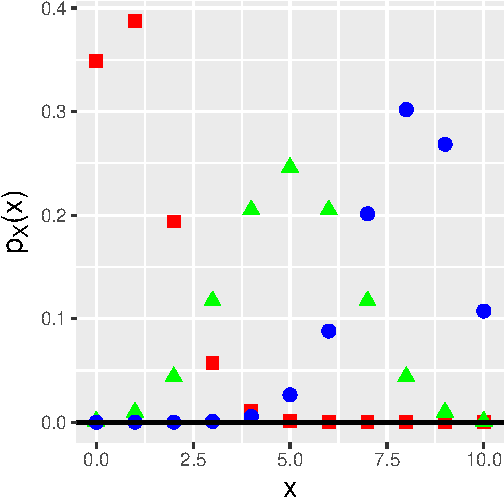
\includegraphics[keepaspectratio]{03-binomial_files/figure-latex/fig-bpmf-1.pdf}}

}

\caption{\label{fig-bpmf}Binomial probability mass functions for number
of trials \(k = 10\) and success probabilities \(p = 0.1\) (red
squares), 0.5 (green triangles), and 0.8 (blue circles).}

\end{figure}%

\smallskip\hrule

\begin{quote}
\textbf{Recall:} \emph{the expected value of a discretely distributed
random variable is} \[
E[X] = \sum_x x p_X(x) \,,
\] \emph{where the sum is over all values of \(x\) within the domain of
the pmf \(p_X(x)\). The expected value is equivalent to a weighted
average, with the weight for each possible value of \(x\) being
\(p_X(x)\).}
\end{quote}

\smallskip\hrule

For the binomial distribution, the expected value is \[
E[X] = \sum_{x=0}^k x \binom{k}{x} p^x (1-p)^{k-x} \,.
\] At first, this does not appear to be easy to evaluate. One trick in
our mathematical arsenal is to pull constants out of the summation such
that whatever is left as the summand is a pmf (and thus sums to 1).
Let's try this here: \begin{align*}
E[X] &= \sum_{x=0}^k x \binom{k}{x} p^x (1-p)^{k-x} = \sum_{x=1}^k x \frac{k!}{x!(k-x)!} p^x (1-p)^{k-x} \\
     &= \sum_{x=1}^k \frac{k!}{(x-1)!(k-x)!} p^x (1-p)^{k-x} \\
     &= kp \sum_{x=1}^k \frac{(k-1)!}{(x-1)!(k-x)!} p^{x-1} (1-p)^{k-x} \,.
\end{align*} The summation appears almost like that of a binomial random
variable. Let's set \(y = x-1\). Then \begin{align*}
E[X] &= kp \sum_{x=1}^k \frac{(k-1)!}{(x-1)!(k-x)!} p^{x-1} (1-p)^{k-x} \\
     &= kp \sum_{y=0}^{k-1} \frac{(k-1)!}{y!(k-(y+1))!} p^y (1-p)^{k-(y+1)} \\
     &= kp \sum_{y=0}^{k-1} \frac{(k-1)!}{y!((k-1)-y)!} p^y (1-p)^{(k-1)-y} \,.
\end{align*} The summand is now the pmf for the random variable
\(Y \sim\) Binomial(\(k-1\), \(p\)), summed over all values of \(y\) in
the domain of the distribution. Thus the summation evaluates to 1, and
\(E[X] = kp\). In an example below, we use a similar strategy to
determine that the variance of a binomial random variable, \(V[X]\), is
equal to \(kp(1-p)\).

\subsection{Examples}\label{examples-26}

\subsubsection{Binomial Random Variable:
Variance}\label{binomial-random-variable-variance}

\smallskip\hrule

\begin{quote}
\textbf{Recall:} \emph{the variance of a discretely distributed random
variable is} \[
V[X] = \sum_x (x-\mu)^2 p_X(x) = E[X^2] - (E[X])^2\,,
\] \emph{where the sum is over all values of \(x\) in the domain of the
pmf \(p_X(x)\). The variance represents the square of the ``width'' of a
probability mass function, where by ``width'' we mean the range of
values of \(x\) for which \(p_X(x)\) is effectively non-zero.}
\end{quote}

\smallskip\hrule

\begin{quote}
The variance of a random variable is given by the shortcut formula that
we have been using since Section~\ref{sec-chap1expected}:
\(V[X] = E[X^2] - (E[X])^2\). So we would expect that we would need to
compute \(E[X^2]\) here, since we already know that \(E[X] = kp\). But
for reasons that will become apparent below, it is actually far easier
for us to compute \(E[X(X-1)]\), and to work with that to eventually
derive the variance: \begin{align*}
E[X(X-1)] &= \sum_{x=0}^k x(x-1) \binom{k}{x} p^x (1-p)^{k-x} \\
&= \sum_{x=0}^k x(x-1) \frac{k!}{x!(k-x)!} p^x (1-p)^{k-x} \\
&= \sum_{x=2}^k \frac{k!}{(x-2)!(k-x)!} p^x (1-p)^{k-x} \\
&= k(k-1) p^2 \sum_{x=2}^k \frac{(k-2)!}{(x-2)!(k-x)!} p^{x-2} (1-p)^{k-x} \,.
\end{align*} The advantage to using \(x(x-1)\) was that it matches the
first two terms of \(x! = x(x-1)\cdots(1)\), allowing easy cancellation.
If we set \(y = x-2\), we find that the summand above will, in a similar
manner as in the calculation of \(E[X]\), become the pmf for the random
variable \(Y \sim\) Binomial(\(k-2,p\))\ldots and thus the summation
will evaluate to 1. Hence \begin{align*}
E[X(X-1)] &= E[X^2] - E[X] = k(k-1)p^2 \\
\Rightarrow ~~~ E[X^2] &= k^2p^2-kp^2 + kp = V[X] + (E[X])^2 \\
\Rightarrow ~~~ V[X] &= k^2p^2-kp^2+kp-k^2p^2 = kp-kp^2 = kp(1-p) \,.
\end{align*}
\end{quote}

\subsubsection{Binomial Distribution: Normal
Approximation}\label{binomial-distribution-normal-approximation}

\begin{quote}
In certain limiting situations, a binomial random variable converges in
distribution to a normal random variable. In other words, if \[
P\left(\frac{X-\mu}{\sigma} < a \right) = P\left(\frac{X-kp}{\sqrt{kp(1-p)}} < a \right) \approx P(Z < a) = \Phi(a) \,,
\] then we can state that
\(X \overset{d}{\rightarrow} Y \sim \mathcal{N}(kp,kp(1-p))\), or that
\(X\) converges in distribution to a normal random variable \(Y\). Now,
what do we mean by ``certain limiting situations''? For instance, if
\(p\) is close to zero or one, then the binomial distribution is
truncated at 0 or at \(k\), and the shape of the pmf does \emph{not}
appear to be like that of a normal pdf. One convention is that the
normal approximation is adequate if \[
k > 9\left(\frac{\mbox{max}(p,1-p)}{\mbox{min}(p,1-p)}\right) \,.
\] The reader might question why we would mention this approximation at
all: if we have binomially distributed data and a computer, then we need
not ever utilize such an approximation to, e.g., compute probabilities.
This point is correct (and is the reason why, for instance, we do not
mention the so-called \emph{continuity correction} here; our goal is not
to compute probabilities). The reason we mention this is that this
approximation underlies a commonly used hypothesis test framework, the
\emph{Wald interval}, that we will mention later in the chapter, in
Section~\ref{sec-chap3confidence}.
\end{quote}

\subsubsection{Binomial Distribution: Exponential
Family}\label{binomial-distribution-exponential-family}

\smallskip\hrule

\begin{quote}
\textbf{Recall:} \emph{the exponential family of distributions is the
set of distributions whose probability mass or density functions can be
expressed as} \[
h(x) \exp\left[\left(\sum_{i=1}^p \eta_i(\boldsymbol{\theta}) T_i(x)\right) - A(\boldsymbol{\theta})\right] \,,
\] \emph{where \(\boldsymbol{\theta}\) is a vector of parameters (e.g.,
\(\boldsymbol{\theta} = \{\mu,\sigma^2\}\) for a normal distribution).
Note that none of the parameters can be a domain-specifying parameter.}
\end{quote}

\smallskip\hrule

\begin{quote}
Is the binomial distribution a member of the exponential family of
distributions? It would initially appear that the answer is no (as there
are no exponential functions in its pmf), but if we note that
\begin{align*}
p^x = \exp\left(\log p^x\right) = \exp\left(x \log p\right)
\end{align*} and that \begin{align*}
(1-p)^{k-x} = \exp\left[\log (1-p)^{k-x}\right] = \exp\left[(k-x) \log (1-p)\right] \,,
\end{align*} we can see that \begin{align*}
p_X(x) = \binom{k}{x} \exp\left( x [ \log(p) - \log(1-p) ] + k \log (1-p) \right)
\end{align*} and thus that \begin{align*}
h(x) &= \binom{k}{x} ~~~~~~ \eta(p) = \log(p) - \log(1-p) = \log \frac{p}{1-p} \\
T(x) &= x ~~~~~~~~~~~ A(p) = -k \log(1-p) \,.
\end{align*} The binomial distribution is indeed a member of the
exponential family.
\end{quote}

\section{Binomial Distribution: Cumulative Distribution
Function}\label{sec-chap3cdf}

What to take away from this section:

\begin{itemize}
\item
  The cumulative distribution function, or cdf, for a binomial
  distribution is a \emph{step function} that can be difficult to work
  with analytically (which historically motivated the application of the
  normal approximation, but which now leads us to use coding for exact
  inference).
\item
  Foreshadowing: the discrete nature of the binomial distribution leads
  to our having to take great care in how we pursue inference\ldots as
  we will see, the question ``do we include a specific probability mass
  in a calculation, or not'' takes on great import when working with
  binomial-related sampling distributions.
\end{itemize}

\smallskip\hrule

\begin{quote}
\textbf{Recall}: \emph{the cumulative distribution function, or cdf, is
another means by which to encapsulate information about a probability
distribution. For a discrete distribution, it is defined as
\(F_X(x) = \sum_{y\leq x} p_Y(y)\), and it is defined for all values
\(x \in (-\infty,\infty)\), with \(F_X(-\infty) = 0\) and
\(F_X(\infty) = 1\).}
\end{quote}

\smallskip\hrule

For the binomial distribution, the cdf is \[
F_X(x) = \sum_{y=0}^{\lfloor x \rfloor} p_Y(y) = \sum_{y=0}^{\lfloor x \rfloor} \binom{k}{y} p^y (1-p)^{k-y} = I_q\left(k - {\lfloor x \rfloor}, 1 + {\lfloor x \rfloor}\right) \,,
\] where \(\lfloor x \rfloor\) denotes the \emph{floor function}, which
returns the largest integer that is less than or equal to \(x\) (e.g.,
if \(x\) = 6.75, \(\lfloor x \rfloor\) = 6). (\(I_q(\cdot)\) is the
regularized incomplete beta function, which is not analytically easy to
work with.) Also, because a pmf is defined at discrete values of \(x\),
its associated cdf is a step function, as illustrated in the left panel
of Figure~\ref{fig-bincdf}. As we can see in this figure, the cdf steps
up at each value of \(x\) in the domain of \(p_X(x)\), and unlike the
case for continuous distributions, the form of the inequalities in a
probabilistic statement matter: \(P(X < x)\) and \(P(X \leq x)\) will
not be the same, if \(x\) is an integer with value
\(\{0,1,2,\ldots,k\}\).

\smallskip\hrule

\begin{quote}
\textbf{Recall}: \emph{an inverse cdf function \(x = F_X^{-1}(q)\) takes
as input a distribution quantile \(q \in [0,1]\) and returns the value
of \(x\). A discrete distribution has no unique inverse cdf; it is
convention to utilize the generalized inverse cdf,} \[
x = \mbox{inf}\{x : F_X(x) \geq q\} \,,
\] \emph{where ``inf'' indicates that the function is to return the
smallest value of \(x\) such that \(F_X(x) \geq q\).}
\end{quote}

\smallskip\hrule

In the right panel of Figure~\ref{fig-bincdf}, we display the inverse
cdf for the same distribution used to generate the figure in the left
panel (\(k=4\) and \(p=0.5\)). Like the cdf, the inverse cdf for a
discrete distribution is a step function. Below, in an example, we show
how we adapt the inverse transform sampler algorithm of
Section~\ref{sec-chap1sample} to accommodate the step-function nature of
an inverse cdf.

\begin{figure}

\begin{minipage}[t]{0.50\linewidth}

\centering{

\pandocbounded{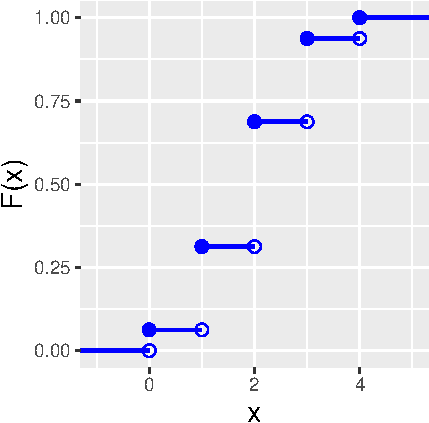
\includegraphics[keepaspectratio]{03-binomial_files/figure-latex/fig-bincdf-1.pdf}}

}

\subcaption{\label{fig-bincdf-1}}

\end{minipage}%
%
\begin{minipage}[t]{0.50\linewidth}

\centering{

\pandocbounded{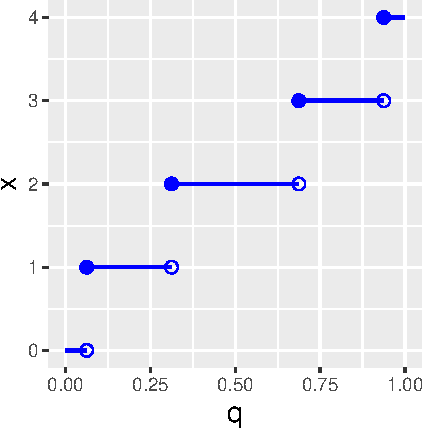
\includegraphics[keepaspectratio]{03-binomial_files/figure-latex/fig-bincdf-2.pdf}}

}

\subcaption{\label{fig-bincdf-2}}

\end{minipage}%

\caption{\label{fig-bincdf}Illustration of the cumulative distribution
function \(F_X(x)\) (a) and inverse cumulative distribution function
\(F_X^{-1}(q)\) (b) for a binomial distribution with number of trials
\(k = 4\) and probability of success \(p=0.5\).}

\end{figure}%

\subsection{Examples}\label{examples-27}

\subsubsection{Computing Probabilities}\label{computing-probabilities-8}

\begin{quote}
Because computing the binomial pmf for a range of values of \(x\) can be
laborious, we typically utilize \texttt{R} functions when computing
probabilities.
\end{quote}

\begin{quote}
\begin{enumerate}
\def\labelenumi{\arabic{enumi}.}
\tightlist
\item
  If \(X \sim\) Binomial(10,0.6), which is \(P(4 \leq X < 6)\)?
\end{enumerate}
\end{quote}

\begin{quote}
We first note that due to the form of the inequality, we do \emph{not}
include \(X=6\) in the computation. Thus
\(P(4 \leq X < 6) = p_X(4) + p_X(5)\), which equals \[
\binom{10}{4} (0.6)^4 (1-0.6)^6 + \binom{10}{5} (0.6)^5 (1-0.6)^5 \,.
\] Even computing this is unnecessarily laborious; instead, we call on
\texttt{R}:
\end{quote}

\begin{Shaded}
\begin{Highlighting}[]
\FunctionTok{round}\NormalTok{(}\FunctionTok{sum}\NormalTok{(}\FunctionTok{dbinom}\NormalTok{(}\DecValTok{4}\SpecialCharTok{:}\DecValTok{5}\NormalTok{, }\AttributeTok{size =} \DecValTok{10}\NormalTok{, }\AttributeTok{prob =} \FloatTok{0.6}\NormalTok{)), }\DecValTok{3}\NormalTok{)}
\end{Highlighting}
\end{Shaded}

\begin{verbatim}
[1] 0.312
\end{verbatim}

\begin{quote}
(This utilizes \texttt{R}'s vectorization feature: we need not
explicitly define a \texttt{for}-loop to evaluate \texttt{dbinom()} for
\(x=4\) and then at \(x=5\).) We can also utilize cdf functions here:
\begin{align*}
P(4 \leq X < 6) &= P(X < 6) - P(X < 4) = P(X \leq 5) - P(X \leq 3)\\
&= F_X(5) - F_X(3) \,,
\end{align*} which in \texttt{R} is computed via
\end{quote}

\begin{Shaded}
\begin{Highlighting}[]
\FunctionTok{round}\NormalTok{(}\FunctionTok{pbinom}\NormalTok{(}\DecValTok{5}\NormalTok{, }\AttributeTok{size =} \DecValTok{10}\NormalTok{, }\AttributeTok{prob =} \FloatTok{0.6}\NormalTok{) }\SpecialCharTok{{-}} \FunctionTok{pbinom}\NormalTok{(}\DecValTok{3}\NormalTok{, }\AttributeTok{size =} \DecValTok{10}\NormalTok{, }\AttributeTok{prob =} \FloatTok{0.6}\NormalTok{), }\DecValTok{3}\NormalTok{)}
\end{Highlighting}
\end{Shaded}

\begin{verbatim}
[1] 0.312
\end{verbatim}

\begin{quote}
As we can see, a direct summation approach is the more straightforward
one to use.
\end{quote}

\begin{quote}
\begin{enumerate}
\def\labelenumi{\arabic{enumi}.}
\setcounter{enumi}{1}
\tightlist
\item
  If \(X \sim\) Binomial(10,0.6), what is the value of \(a\) such that
  \(P(X \leq a) = 0.9\)?
\end{enumerate}
\end{quote}

\begin{quote}
First, we set up the inverse cdf formula: \[
P(X \leq a) = F_X(a) = 0.9 ~~ \Rightarrow ~~ a = F_X^{-1}(0.9)
\] Note that we didn't do anything differently here than we would have
done in a continuous distribution setting\ldots and we can proceed
directly to \texttt{R} because it utilizes the generalized inverse cdf
algorithm.
\end{quote}

\begin{Shaded}
\begin{Highlighting}[]
\FunctionTok{qbinom}\NormalTok{(}\FloatTok{0.9}\NormalTok{, }\AttributeTok{size =} \DecValTok{10}\NormalTok{, }\AttributeTok{prob =} \FloatTok{0.6}\NormalTok{)}
\end{Highlighting}
\end{Shaded}

\begin{verbatim}
[1] 8
\end{verbatim}

\begin{quote}
We can see immediately how the cdf for a discrete distribution is not a
one-to-one function, as when we plug \(x = 8\) into the cdf, we will not
recover the initial value \(q = 0.9\) (but, rather, a larger value):
\end{quote}

\begin{Shaded}
\begin{Highlighting}[]
\FunctionTok{round}\NormalTok{(}\FunctionTok{pbinom}\NormalTok{(}\DecValTok{8}\NormalTok{, }\AttributeTok{size =} \DecValTok{10}\NormalTok{, }\AttributeTok{prob =} \FloatTok{0.6}\NormalTok{), }\DecValTok{3}\NormalTok{)}
\end{Highlighting}
\end{Shaded}

\begin{verbatim}
[1] 0.954
\end{verbatim}

\subsubsection{Probability Mass Functions: Data
Sampling}\label{probability-mass-functions-data-sampling}

\begin{quote}
While we would always utilize \texttt{R} shortcut functions like
\texttt{rbinom()} when they exist, there may be instances when we need
to code our own functions for sampling data from discrete distributions.
The code below shows such a function for an arbitrary probability mass
function; we can easily adapt this code to any situation in which a pmf
and its domain are concisely specified.
\end{quote}

\begin{Shaded}
\begin{Highlighting}[]
\FunctionTok{set.seed}\NormalTok{(}\DecValTok{101}\NormalTok{)}
\NormalTok{x   }\OtherTok{\textless{}{-}} \FunctionTok{c}\NormalTok{(}\DecValTok{1}\NormalTok{, }\DecValTok{2}\NormalTok{, }\DecValTok{4}\NormalTok{, }\DecValTok{8}\NormalTok{)              }\CommentTok{\# domain of x}
\NormalTok{p.x }\OtherTok{\textless{}{-}} \FunctionTok{c}\NormalTok{(}\FloatTok{0.2}\NormalTok{, }\FloatTok{0.35}\NormalTok{, }\FloatTok{0.15}\NormalTok{, }\FloatTok{0.3}\NormalTok{)    }\CommentTok{\# p\_X(x)}
\NormalTok{F.x }\OtherTok{\textless{}{-}} \FunctionTok{cumsum}\NormalTok{(p.x)                }\CommentTok{\# cumulative sum {-}\textgreater{} produces F\_X(x)}
\NormalTok{n   }\OtherTok{\textless{}{-}} \DecValTok{100}
\NormalTok{q   }\OtherTok{\textless{}{-}} \FunctionTok{runif}\NormalTok{(n)                   }\CommentTok{\# we still ultimately need runif!}
\NormalTok{i   }\OtherTok{\textless{}{-}} \FunctionTok{findInterval}\NormalTok{(q, F.x) }\SpecialCharTok{+} \DecValTok{1}   \CommentTok{\# the output are bin numbers [0,3], and not [1,4]}
                                  \CommentTok{\# hence we add 1}
                                  \CommentTok{\# 1 means q is between 0 and F.x[1], etc.}
\NormalTok{x.sample }\OtherTok{\textless{}{-}}\NormalTok{ x[i]}
\end{Highlighting}
\end{Shaded}

\begin{figure}

\centering{

\pandocbounded{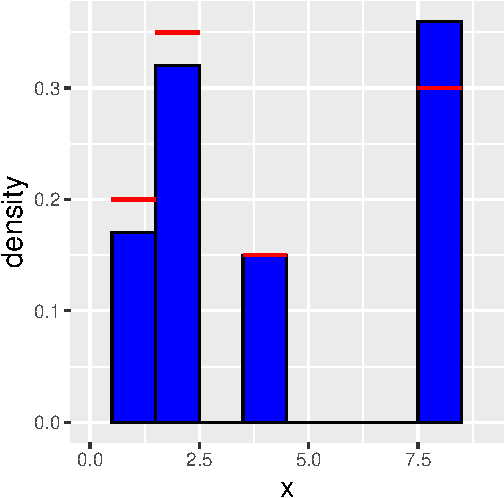
\includegraphics[keepaspectratio]{03-binomial_files/figure-latex/fig-pmfsamp-1.pdf}}

}

\caption{\label{fig-pmfsamp}Histogram of \(n = 100\) iid data drawn
using an inverse tranform sampler adapted to the discrete distribution
setting. The red lines indicate the true density for each value of
\(x\).}

\end{figure}%

\section{Binomial-Related Distributions}\label{sec-chap3related}

What to take away from this section:

\begin{itemize}
\item
  There are several distributions related to the binomial distribution
  that are often seen in data analyses\ldots{}

  \begin{itemize}
  \item
    the \emph{negative binomial} and \emph{geometric} distributions, in
    which the random variable is the number of failures and the number
    of successes is fixed;
  \item
    the \emph{hypergeometric} distribution, which governs binomial-like
    trials in which data are sampled from finite tangible populations,
    without replacement;
  \item
    the \emph{multinomial} distribution, for which the number of
    outcomes is \(> 2\); and
  \item
    the \emph{beta} distribution, a continuous bounded distribution that
    one can use to model the binomial success proportion \(p\).
  \end{itemize}
\end{itemize}

There are several probability distributions that are directly related to
the binomial distribution and that are commonly utilized in statistical
inference. Some of these are

\begin{itemize}
\tightlist
\item
  the \emph{negative binomial} and \emph{geometric} distributions;
\item
  the \emph{hypergeometric} distribution;
\item
  the \emph{multinomial} distribution; and
\item
  the \emph{beta} distribution.
\end{itemize}

Below, we introduce each in turn.

\subsection{Negative Binomial and Geometric
Distributions}\label{sec-chap3nb}

A closely related alternative to a binomial experiment is a negative
binomial experiment, in which the number of successes \(s\) is fixed in
advance, as opposed to the number of trials \(k\). A simple example of
such an experiment would be flipping a coin until we observe \(s\)
heads. The random variable of interest is then the number of failures
that we observe before achieving the last success (here, the number of
observed tails).

The negative binomial distribution has probability mass function \[
p_X(x) = \binom{x+s-1}{x} p^s (1-p)^x ~~~ x \in \{0,1,\ldots,\infty\} \,.
\] The form of this pmf follows from the fact that the underlying
Bernoulli process would consist of \(x+s\) data, with the last datum
being the observed success that ends the experiment. The first \(x+s-1\)
data would feature \(s-1\) successes and \(x\) failures, with the order
of success and failure not mattering\ldots so we can view these data as
being binomially distributed (albeit with \(x\) representing
failures\ldots hence the ``negative'' in negative binomial!): \[
p_X(x) = \underbrace{\binom{x+s-1}{x} p^{s-1} (1-p)^x}_{\mbox{first $x+s-1$ trials}} \cdot \underbrace{p}_{\mbox{last trial}} \,.
\] Setting \(s = 1\) yields the geometric distribution, with probability
mass function \[
p_X(x) = p (1-p)^x ~~~ x \in \{0,1,\ldots,\infty\} \,.
\]

As stated above, \(X\) represents the number of failures in a negative
binomial experiment. Alternatively, \(X\) can represent the overall
number of trials in an experiment (i.e., the number of failures plus the
number of successes). Adopting either representation ultimately yields
the same statistical inferences for the success probability \(p\). Here,
we choose to follow how the negative binomial pmf is defined in
\texttt{R}.

\begin{figure}

\centering{

\pandocbounded{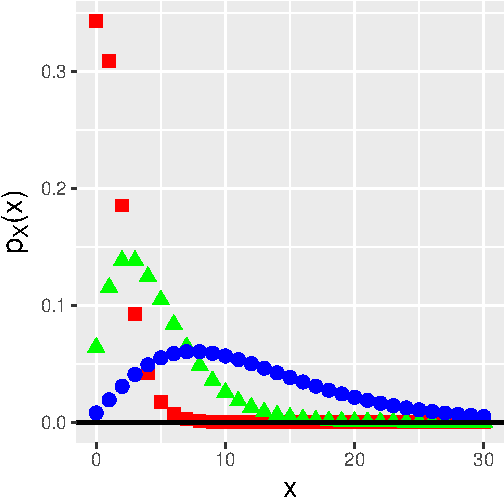
\includegraphics[keepaspectratio]{03-binomial_files/figure-latex/fig-nbpmf-1.pdf}}

}

\caption{\label{fig-nbpmf}Negative binomial probability mass functions
for the number of successes \(s = 2\) and success probabilities
\(p = 0.7\) (red squares), 0.5 (green triangles), and 0.2 (blue
circles).}

\end{figure}%

\subsection{Hypergeometric Distribution}\label{sec-chap3hyper}

Imagine that we are given \(K = 100\) widgets, of which ten are
defective. This set of widgets comprises a finite, tangible population.
If we were to sample \(k\) widgets \emph{with replacement}, then the
observed number of defective ones would be a binomially distributed
random variable. However, a more typical situation would be one in which
we grab a widget, check it to see if it is defective, and then \emph{set
it aside}\ldots then grab and check another and then \emph{set that
widget aside}\ldots etc. Perhaps we continue this process until all ten
defective widgets are found. In this situation, we are sampling
\emph{without replacement}, and because of that, the probability of
``success'' (i.e., finding a defective widget) changes from an initial
value of \(0.1\) to either \(0.091\) or \(0.101\), etc. Thus we are not
carrying out a binomial experiment; rather, we are carrying out a
hypergeometric experiment, where the data are governed by the
hypergeometric distribution.

Assume that we draw \(k\) samples from a population of size \(K\), in
which there are \(s\) ``success'' objects and \(K-s\) ``failure''
objects. The probability of observing \(X = x\) successes is \[
p_X(x) = \frac{\binom{s}{x} \binom{K-s}{k-x}}{\binom{K}{k}} \,,
\] where \(x \in \{0, \ldots, {\mathrm{min}}(k,s)\}\). The expected
value and variance are \begin{align*}
E[X] &= \frac{ks}{K} \\
V[X] &= k \frac{s}{K} \frac{K-s}{K} \frac{K-k}{K-1} \,.
\end{align*}

Historical convention holds that one can utilize the binomial
distribution to model hypergeometric data if the number of trials
\(k \lesssim K/10\). (This is the so-called ``10\% rule'' of
introductory statistics.) \emph{However, in the age of computers, there
is no reason to do this\ldots it is simple to apply the exact
distribution instead.}

\subsection{Multinomial Distribution}\label{sec-chap3multi}

The multinomial distribution is a generalization of the binomial
distribution that we apply in situations in which each trial has more
than two outcomes. The properties of a multinomial experiment are the
following.

\begin{enumerate}
\def\labelenumi{\arabic{enumi}.}
\tightlist
\item
  It consists of \(k\) trials, with \(k\) chosen in advance.
\item
  There are \(m\) possible outcomes for each trial.
\item
  A trial may have no more than one realized outcome.
\item
  The outcomes of each trial are independent.
\item
  The probability of achieving the \(i^{th}\) outcome is \(p_i\), a
  quantity that remains constant throughout the experiment.
\item
  The probabilities of each outcome sum to one:
  \(\sum_{i=1}^m p_i = 1\).
\item
  The number of trials that achieve a particular outcome is \(X_i\),
  with \(\sum_{i=1}^m X_i = k\).
\end{enumerate}

The probability of any single experimental outcome
\(\{X_1,\ldots,X_m\}\) is given by the multinomial probability mass
function: \[
p(x_1,\ldots,x_m \vert p_1,\ldots,p_m) = \frac{k!}{x_1! \cdots x_m!}p_1^{x_1}\cdots p_m^{x_m} \,.
\] The distribution for any one value \(X_i\) is binomial, with
\(E[X_i] = kp_i\) and \(V[X_i] = kp_i(1-p_i)\). This makes intuitive
sense, as one either observes \(i\) as a trial outcome (success), or
observes something else (failure). However, the \(X_i\)'s are \emph{not}
independent random variables; the covariance between \(X_i\) and
\(X_j\), a metric of linear dependence, is not zero but rather
\(-kp_ip_j\) if \(i \neq j\). (We will discuss the concept of covariance
in Section~\ref{sec-chap6covariance}.) This also makes intuitive sense:
given that the number of trials \(k\) is fixed, observing more data
having one outcome will usually mean observing fewer data achieving any
other outcome.

\subsection{Beta Distribution}\label{sec-chap3beta}

The beta distribution is a continuous distribution that is commonly used
to model random variables with finite, bounded domains. Its probability
density function is given by \[
f_X(x) = \frac{x^{a-1}(1-x)^{b-1}}{B(a,b)} \,,
\] where \(x \in [0,1]\), \(a\) and \(b\) are both \(> 0\), and the
normalization constant \(B(a,b)\) is \[
B(a,b) = \int_0^1 x^{a-1}(1-x)^{b-1} dx = \frac{\Gamma(a)\Gamma(b)}{\Gamma(a+b)} \,.
\] (See Figure~\ref{fig-betapdf}.) We have seen the gamma function,
\(\Gamma(u)\), before; it is defined as \[
\Gamma(u) = \int_0^\infty x^{u-1} e^{-x} dx \,.
\] There are two things to note about the gamma function. The first is
its \emph{recursive property}: \(\Gamma(u+1) = u \Gamma(u)\).\\
(This can be shown by applying integration by parts.) The second is that
when \(u\) is a positive integer, the gamma function takes on the value
\((u-1)! = (u-1)(u-2) \cdots 1\). (Note that \(\Gamma(1) = 0! = 1\).)

Regarding the statement above about ``model{[}ing{]} random variables
with finite, bounded domains'': if a set of \(n\) iid random variables
\(\mathbf{X}\) has domain \([c,d]\), we can define a new set of random
variables \(\mathbf{Y}\) via the transformation \[
\mathbf{Y} = \frac{\mathbf{X}-c}{d-c}
\] such that the domain becomes \([0,1]\). We can then model the
transformed data with the beta distribution. (Note the word \emph{can}:
we can model these data with the beta distribution, but we don't have
to, and it may be the case that there is another distribution bounded on
the interval \([0,1]\) that ultimately better describes the
data-generating process. The beta distribution just happens to be the
one analysts most commonly use.)

But\ldots in the end, what does this all have to do with the binomial
distribution, the subject of this chapter? We know the binomial has a
parameter \(p \in [0,1]\) and the domain of the beta distribution is
\([0,1]\), but is there more? Let's write down the binomial pmf: \[
\binom{k}{x} p^x (1-p)^{k-x} = \frac{k!}{x!(k-x)!} p^x (1-p)^{k-x} \,.
\] This pmf dictates the probability of observing a particular value of
\(x\) given \(k\) and \(p\). But what if we turn this around a
bit\ldots and examine this function if we fix \(k\) and \(x\) and vary
\(p\) instead? In other words, let's examine the likelihood function \[
\mathcal{L}(p \vert k,x) = \frac{k!}{x!(k-x)!} p^x (1-p)^{k-x} \,.
\] We can see immediately that the likelihood has the form of a beta
distribution if we set \(a = x+1\) and \(b = k-x+1\): \[
\mathcal{L}(p \vert k,x) = \frac{\Gamma(a+b-1)}{\Gamma(a)\Gamma(b)} p^{a-1} (1-p)^{b-1} \,,
\] \emph{except} that the normalization term is not quite right: here we
have \(\Gamma(a+b-1)\) instead of \(\Gamma(a+b)\). But that's fine:
there is no requirement that a likelihood function integrate to one over
its domain. (Here, as the interested reader can verify, the likelihood
function integrates to \(1/(k+1)\).) So, in the end, if we observe a
random variable \(X \sim\) Binomial(\(k,p\)), then the likelihood
function \(\mathcal{L}(p \vert k,x)\) has the shape (if not the
normalization) of a Beta(\(x+1,k-x+1\)) distribution.

\begin{figure}

\centering{

\pandocbounded{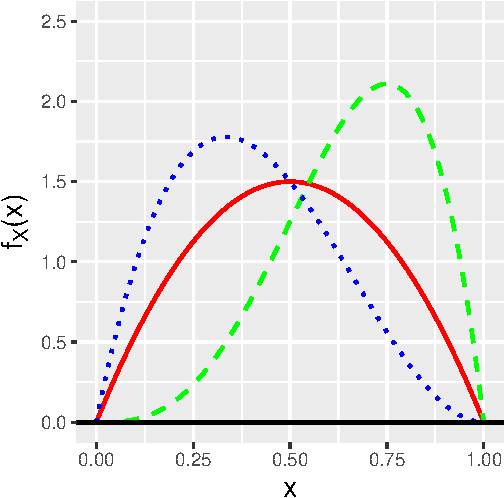
\includegraphics[keepaspectratio]{03-binomial_files/figure-latex/fig-betapdf-1.pdf}}

}

\caption{\label{fig-betapdf}Three examples of beta probability density
functions: Beta(2,2) (solid red line), Beta(4,2) (dashed green line),
and Beta(2,3) (dotted blue line).}

\end{figure}%

\subsection{Examples}\label{examples-28}

\subsubsection{Negative Binomial Random Variable: Expected
Value}\label{negative-binomial-random-variable-expected-value}

\begin{quote}
The calculation for the expected value \(E[X]\) for a negative binomial
random variable is similar to that for a binomial random variable:
\begin{align*}
E[X] &= \sum_{x=0}^{\infty} x \binom{x+s-1}{x} p^s (1-p)^x \\
&= \sum_{x=0}^{\infty} x \frac{(x+s-1)!}{(s-1)!x!} p^s (1-p)^x \\
&= \sum_{x=1}^{\infty} \frac{(x+s-1)!}{(s-1)!(x-1)!} p^s (1-p)^x \,.
\end{align*} Let \(y = x-1\). Then \begin{align*}
E[X] &= \sum_{y=0}^{\infty} \frac{(y+s)!}{(s-1)!y!} p^s (1-p)^{y+1} \\
&= \sum_{y=0}^{\infty} s(1-p) \frac{(y+s)!}{s!y!} p^s (1-p)^y \\
&= \sum_{y=0}^{\infty} \frac{s(1-p)}{p} \frac{(y+s)!}{s!y!} p^{s+1} (1-p)^y \\
&= \frac{s(1-p)}{p} \sum_{y=0}^{\infty} \frac{(y+s)!}{s!y!} p^{s+1} (1-p)^y = \frac{s(1-p)}{p} \,.
\end{align*} The summand is that of a negative binomial distribution for
\(s+1\) successes, hence the summation is 1, and thus
\(E[X] = s(1-p)/p\).
\end{quote}

\begin{quote}
We leave it as an exercise to the reader to carry out a similar
calculation, that involves evaluating \(E[X(X-1)]\), to derive the
variance of a negative binomial random variable: \(V[X] = s(1-p)/p^2\).
\end{quote}

\subsubsection{Beta Random Variable: Expected
Value}\label{beta-random-variable-expected-value}

\begin{quote}
The expected value of a random variable sampled from a Beta(\(a,b\))
distribution is \begin{align*}
E[X] &= \int_0^1 x f_X(x) dx = \int_0^1 x \frac{x^{a-1} (1-x)^{b-1}}{B(a,b)} dx \\
&= \int_0^1 \frac{x^{a} (1-x)^{b-1}}{B(a,b)} dx = \int_0^1 \frac{x^{a} (1-x)^{b-1}}{B(a+1,b)} \frac{B(a+1,b)}{B(a,b)} dx \\
&= \frac{B(a+1,b)}{B(a,b)} \int_0^1 \frac{x^{a} (1-x)^{b-1}}{B(a+1,b)} dx = \frac{B(a+1,b)}{B(a,b)} \,.
\end{align*} The last result follows from the fact that the integrand is
the pdf for a Beta(\(a+1,b\)) distribution, and the integral is over the
entire domain, hence the integral evaluates to 1.
\end{quote}

\begin{quote}
Continuing, \begin{align*}
E[X] &= \frac{B(a+1,b)}{B(a,b)} = \frac{\Gamma(a+1) \Gamma(b)}{\Gamma(a+b+1)} \frac{\Gamma(a+b)}{\Gamma(a)\Gamma(b)} \\
&= \frac{a \Gamma(a)}{(a+b)\Gamma(a+b)} \frac{\Gamma(a+b)}{\Gamma(a)} = \frac{a}{a+b} \,.
\end{align*} Here, we take advantage of the recursive property of the
gamma function.
\end{quote}

\begin{quote}
The reader can utilize a similar strategy to determine the variance of a
beta random variable, starting by computing \(E[X^2]\) and utilizing the
shortcut formula \(V[X] = E[X]^2 - (E[X])^2\). The final result is \[
V[X] = \frac{ab}{(a+b)^2(a+b+1)} \,.
\]
\end{quote}

\section{Linear Functions of Binomial Random
Variables}\label{sec-chap3linear}

What to take away from this section:

\begin{itemize}
\item
  The \emph{method of moment-generating functions} allows us to
  determine that\ldots{}

  \begin{itemize}
  \item
    the sum of \(n\) iid binomial random variables is itself binomially
    distributed; and
  \item
    the mean of \(n\) iid binomial random variables has a known but
    typically unutilized distribution: it is the sample sum distribution
    with a transformed domain.
  \end{itemize}
\item
  Foreshadowing: the sample sum result will allow us to make statistical
  inferences about the binomial success proportion \(p\), given \(n\)
  iid normal random variables (and that \(k\) is fixed and known).
\end{itemize}

For previous material on sampling distributions, see
Section~\ref{sec-chap2methodmgf}.

Let's assume we are given \(n\) iid binomial random variables:
\(X_1,X_2,\ldots,X_n \sim\) Binomial(\(k\),\(p\)). Can we determine the
distribution of \(Y = \sum_{i=1}^n a_i X_i\)? Yes, we can\ldots via the
method of moment-generating functions.

\smallskip\hrule

\begin{quote}
\textbf{Recall}: \emph{the moment-generating function, or mgf, is a
means by which to encapsulate information about a probability
distribution. When it exists, the mgf is given by
\(m_X(t) = E[e^{tX}]\). Also, if \(Y = \sum_{i=1}^n a_iX_i\), then
\(m_Y(t) = m_{X_1}(a_1t) m_{X_2}(a_2t) \cdots m_{X_n}(a_nt)\); if we can
identify \(m_Y(t)\) as the mgf for a known family of distributions, then
we can immediately identify the distribution for \(Y\) and the
parameters of that distribution.}
\end{quote}

\smallskip\hrule

The mgf for the binomial distribution is \begin{align*}
m_X(t) = E[e^{tX}] &= \sum_{x=0}^k e^{tx} \binom{k}{x} p^x (1-p)^{k-x} \\
                   &= \sum_{x=0}^k \binom{k}{x} (pe^t)^x (1-p)^{k-x} \,.
\end{align*} To achieve a closed-form expression, we utilize the
binomial theorem: \[
(x+y)^k = \sum_{i=0}^k \binom{k}{i} x^i y^{k-i}
\] to re-express \(m_X(t)\): \[
m_X(t) = [pe^t + (1-p)]^k \,.
\] Note that one may see this written elsewhere as \((pe^t+q)^k\), where
\(q = 1-p\).

The mgf for \(Y = X_+ = \sum_{i=1}^n X_i\) is thus \[
m_Y(t) = \prod_{i=1}^n m_{X_i}(t) = [m_X(t)]^n = [pe^t + (1-p)]^{nk} \,.
\] We can see that this has the form of a binomial mgf: \(Y \sim\)
Binomial(\(nk\),\(p\)), with expected value \(E[Y] = nkp\) and variance
\(V[Y] = nkp(1-p)\). This makes sense, as the act of summing binomial
data is equivalent to concatenating \(n\) separate Bernoulli processes
into one longer Bernoulli process\ldots whose data can subsequently be
modeled using a binomial distribution.

While we can identify the distribution of the sum by name, we cannot say
the same about the sample mean. We know that the expected value is
\(E[\bar{X}] = \mu = kp\) and that the variance is
\(V[\bar{X}] = \sigma^2/n = kp(1-p)/n\), but when we attempt to use the
mgf method with \(a_i = 1/n\) instead of \(a_i = 1\), we find that \[
m_{\bar{X}}(t) = [pe^{t/n} + (1-p)]^{nk} \,.
\] Changing \(t\) to \(t/n\) has the effect of creating an mgf that does
not have the form of any known mgf. However, we \emph{do} know the
details of the distribution: its pmf is identical to that of the
binomial distribution, but its domain is \(\{0,1/n,2/n,\ldots,k\}\)
rather than \(\{0,1,\ldots,nk\}\). (We can derive this result by making
the transformation \(X_+ \rightarrow X_+/n\), as we see below in an
example.) We could define the sample mean cdf ourselves using our own
\texttt{R} function, as in, e.g.,

\begin{Shaded}
\begin{Highlighting}[]
\NormalTok{pbsm }\OtherTok{\textless{}{-}} \ControlFlowTok{function}\NormalTok{(x, k, p, n)  }\CommentTok{\#  bsm: binomial sample mean}
\NormalTok{\{}
  \FunctionTok{return}\NormalTok{(}\FunctionTok{pbinom}\NormalTok{(x }\SpecialCharTok{*}\NormalTok{ n, }\AttributeTok{size =}\NormalTok{ n }\SpecialCharTok{*}\NormalTok{ k, }\AttributeTok{prob =}\NormalTok{ p)}
\ErrorTok{\}}
\end{Highlighting}
\end{Shaded}

However, there is no particular need to do this: as we will see, if we
wish to construct a confidence interval for \(p\), we can just use
\(X_+\) as our statistic, and we will get the same result as if we had
used the sample mean. (We note, for completeness, that we could also
utilize the Central Limit Theorem if \(n \gtrsim 30\), but as we know
the sampling distributions of \(X_+\) and \(\bar{X}\) there is no need
to fall back upon approximations.)

\subsection{Examples}\label{examples-29}

\subsubsection{Geometric Random Variable: Moment-Generating
Function}\label{geometric-random-variable-moment-generating-function}

\begin{quote}
Recall that a geometric distribution is equivalent to a negative
binomial distribution with number of successes \(s = 1\); its
probability mass function is \[
p_X(x) = p (1-p)^x \,,
\] with \(x = \{0,1,\ldots\}\) and \(p \in [0,1]\). The
moment-generating function for a geometric random variable is thus
\begin{align*}
m_X(t) = E[e^{tX}] &= \sum_{x=0}^{\infty} e^{tx} p (1-p)^x = p \sum_{x=0}^\infty e^{tx} (1-p)^x \\
&= p \sum_{x=0}^\infty [e^t(1-p)]^x = \frac{p}{1-e^t(1-p)} \,.
\end{align*} The last equality utilizes the formula for the sum of an
infinite geometric series: \(\sum_{i=0}^\infty x^i = (1-x)^{-1}\), when
\(\vert x \vert < 1\). (If \(t < 0\) and \(p > 0\), then the condition
that \(\vert e^t(1-p) \vert < 1\) holds.)
\end{quote}

\begin{quote}
The sum of \(s\) iid geometric random variables has the
moment-generating function \[
m_Y(t) = \prod_{i=1}^s m_{X_i}(t) = \left[ m_X(t) \right]^n = \left[\frac{p}{1-e^t(1-p)}\right]^s \,.
\] This is the mgf for a negative binomial distribution for \(s\)
successes. In the same way that the sum of \(k\) Bernoulli random
variables is a binomially distributed random variable, the sum of \(s\)
geometric random variables is a negative binomially distributed random
variable.
\end{quote}

\subsubsection{Binomial Data: Sample Mean
Distribution}\label{binomial-data-sample-mean-distribution}

\begin{quote}
Let's assume we are given \(n\) iid binomial random variables:
\(X_1,X_2,\ldots,X_n \sim\) Binomial(\(k\),\(p\)). As we observe above,
the distribution of the sum \(X_+ = \sum_{i=1}^k X_i\) is binomial with
mean \(nkp\) and variance \(nkp(1-p)\).
\end{quote}

\begin{quote}
The sample mean is \(\bar{X} = X_+/n\), and so \[
F_{\bar{X}}(\bar{x}) = P(\bar{X} \leq \bar{x}) = P(X_+ \leq n\bar{x}) = \sum_{x_+=0}^{n\bar{x}} p_{X_+}(x_+) \,.
\] Because \(n\bar{x}\) is integer-valued by definition, we do not need
to round down here. Since we are dealing with a discrete distribution
and not a continuous one, we cannot simply take the derivative of
\(F_{\bar{X}}(\bar{x})\) to find \(f_{\bar{X}}(\bar{x})\)\ldots but what
we can do is assess the jump in the cumulative distribution function at
each step, because that \emph{is} the pmf. We find that \[
f_{\bar{X}}(\bar{x}) = P(X_+ \leq n\bar{x}) - P(X_+ \leq n\bar{x}-1) = f_{X_+}(x_+) = f_{X_+}(n\bar{x})\,.
\] In other words, the pmf for \(\bar{X}\) is equivalent to that for
\(X_+\), just with a different domain (\({0,1/n,2/n,\ldots,k}\) versus
\({0,1,\ldots,nk}\).
\end{quote}

\subsubsection{Probability Generating
Functions}\label{probability-generating-functions}

\begin{quote}
Moment-generating functions are not the only means by which we can work
with linear functions of discrete random variables. Another method is
that of \emph{probability generating functions}, or pgfs, in which we
utilize the Law of the Unconcious Statistician to create power-series
representations of probability mass functions: \[
g_X(t) = E[t^X] = \sum_{x=0}^\infty t^x p_X(x) \,.
\] (Mathematicians would call this a \emph{Mellin transform}.) We note
immediately that we can only compute pgfs for distributions whose
domains consist of the full set of, or a subset of, the values
\(\{0,1,\ldots,\infty\}\). (For instance, the binomial distribution has
domain \(\{0,1,\ldots,k\}\), so \(p_X(k+1) = p_X(k+2) = \cdots = 0\).)
\end{quote}

\begin{quote}
What is the pgf for a binomial distribution? \begin{align*}
g_X(t) &= \sum_{x=0}^k t^x p_X(x) \\
&= \sum_{x=0}^k t^x \binom{k}{x} p^x (1-p)^{k-x} \\
&= \sum_{x=0}^k \binom{k}{x} (tp)^x (1-p)^{k-x} \\
&= \left[ tp + (1-p) \right]^k \,,
\end{align*} where in the last step we utilize the binomial theorem to
achieve a closed-form expression for \(g_X(t)\).
\end{quote}

\begin{quote}
What is the pgf good for? First, we can use a pgf to compute a
\emph{factorial moment}: \(\mu_{[i]} = E[X(X-1) \cdots (X-i+1)]\).
(Earlier, we used the factorial moment \(E[X(X-1)]\) of the binomial
distribution to compute the variance of binomial random variables.) We
can compute such a moment from \(g_X(t)\) as follows: \[
E[X(X-1) \cdots (X-i+1)] = \mu_{[i]} = \left. \frac{d^j}{dt^j} g_X(t) \right|_{t=1} \,.
\] For instance, we found that \(E[X(X-1)] = k(k-1)p^2\) for a binomial
distribution, by playing tricks with summations. With the pgf, we find
that \begin{align*}
\left. \frac{d^2}{dt^2} \left[ tp + (1-p) \right]^k \right|_{t=1} &= \left. \frac{d}{dt} k \left[ tp + (1-p) \right]^{k-1} p \right|_{t=1} \\
&= \left. k (k-1) \left[ tp + (1-p) \right]^{k-2} p^2 \right|_{t=1} \\
&= k (k-1) p^2 \left[ p + (1-p) \right]^{k-2} = k(k-1)p^2 \,.
\end{align*}
\end{quote}

\begin{quote}
Second, we can use a pgf to generate probability mass function values:
\[
p_X(i) = \left. \frac{1}{i!} \frac{d^j}{dt^j} g_X(t) \right|_{t=0} \,.
\] Hence, for a binomial distribution, \begin{align*}
p_X(1) &= \left. \frac{d}{dt} \left[ tp + (1-p) \right]^k \right|_{t=0} \\
&= \left. k \left[ tp + (1-p) \right]^{k-1} p \right|_{t=0} \\
&= k p (1-p)^{k-1} \,,
\end{align*} etc. While this might not seem particularly useful at first
glance, if \(\{X_1,\ldots,X_n\}\) are \(n\) independent (but not
necessarily identically distributed) discrete random variables, and if
\(Y = \sum_{i=1}^n a_i X_i\), then \[
g_Y(t) = g_{X_1}(t^{a_1}) g_{X_2}(t^{a_2}) \cdots g_{X_n}(t^{a_n}) \,,
\] and one can use, e.g., symbolic differentiation to determine the full
probability mass function for \(Y\), if one cannot just recognize
\(Y\)'s distribution. (For instance, if
\(X_1,X_2 \sim \mbox{Binom}(k,p)\), then the pgf for \(Y = X_1 + X_2\)
is \([tp + (1-p)]^{k+k}\), meaning that \(Y \sim \mbox{Binom}(2k,p)\).
\end{quote}

\begin{quote}
To be clear: in the context of this book, probability-generating
functions do not offer any utility to the reader that moment-generating
functions don't already provide. (Their primary advantage is to allow us
to compute pmfs for less straightforward linear functions of discrete
random variables, which is useful to know\(-\)this allows us to perform
statistical inference given such statistics\(-\)but doing this is beyond
the book's current scope.)
\end{quote}

\section{Order Statistics}\label{sec-chap3order}

What to take away from this section:

\begin{itemize}
\item
  \emph{Order statistics} are the observed data of our sample sorted
  into ascending order: e.g., \(X_{(1)}\) is the datum with the smallest
  observed value, and \(X_{(n)}\) is the datum with the largest observed
  value.
\item
  The properties of the binomial distribution allow us to derive the
  probability mass or density function (and cumulative distribution
  function) for an order statistic.
\item
  Foreshadowing: by being able to express the cdf of an order statistic,
  we are in a position to, e.g., make statistical inferences about a
  distribution parameter \(\theta\) using the sample median or the
  sample range.
\end{itemize}

Let's suppose that we have sampled \(n\) iid random variables
\(\{X_1,\ldots,X_n\}\) from some arbitrary distribution. Previously, we
have summarized such data with the sample mean and the sample variance.
However, there are other summary statistics, some of which are only
calculable if we sort the data into ascending order:
\(\{X_{(1)},\ldots,X_{(n)}\}\). These are dubbed \emph{order statistics}
and the \(j^{th}\) order statistic is the sample's \(j^{th}\) smallest
value (i.e., the smallest-valued datum in the sample is \(X_{(1)}\) and
the largest-valued datum is \(X_{(n)}\)). Examples of statistics based
on ordering include \begin{align*}
\mbox{Range:}& ~~X_{(n)} - X_{(1)} \\
\mbox{Median:}& ~~X_{(n+1)/2} ~ \mbox{if $n$ is odd} \\
& ~~(X_{n/2}+X_{(n+1)/2})/2 ~ \mbox{if $n$ is even} \,.
\end{align*} The most important point to keep in mind is that the
probability mass and density functions for order statistics differ from
the pmfs and pdfs for their constituent iid data. For instance, if we
sample \(n\) data from a \(\mathcal{N}(0,1)\) distribution, we would not
expect the minimum value to be distributed the same way; if anything,
the mean should take on smaller and smaller values, and the variance of
those values should decrease, as \(n\) increases.

So: why are we discussing order statistics here, in the middle of a
discussion of the binomial distribution? It is because we can derive,
e.g., the cdf for an order statistic by utilizing the binomial
probability mass function.

\begin{figure}

\centering{

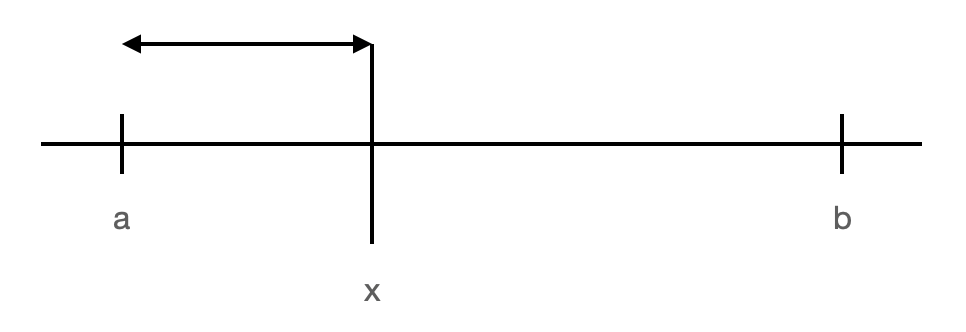
\includegraphics[width=0.75\linewidth,height=\textheight,keepaspectratio]{figures/order.png}

}

\caption{\label{fig-order}If we have, e.g., a probability density
function \(f_X(x)\) whose domain is \([a, b]\), and we view success as
sampling a datum less than a given value \(x\), then when we sample
\(n\) data, the number that have values \(\leq x\) is a binomial random
variable with \(k = n\) and \(p = F_X(x)\).}

\end{figure}%

See Figure~\ref{fig-order}. Without loss of generality, we can assume
that \(f_X(x) > 0\) for \(x \in [a,b]\) and that we sample \(n\) data
from this distribution. The number of data \(X\) that have value less
than some arbitrarily chosen \(x\) is a binomial random variable: \[
Y \sim \mbox{Binomial}(n,p=F_X(x))
\] What is the probability that the \(j^{th}\) ordered datum has a value
\(\leq x\)? That's equivalent to asking for the probability that
\(Y \geq j\), i.e., did we see at least \(j\) successes in \(n\) trials?
\[
F_{(j)}(x) = P(X_{(j)} \leq x) = P(Y \geq j) = \sum_{i=j}^n \binom{n}{i} [F_X(x)]^i [1 - F_X(x)]^{n-i} \,.
\] \(F_{(j)}(x)\) is the cdf for the \(j^{th}\) ordered datum.

What is \(f_{(j)}(x)\) if \(X\) is a continuous random variable?

\smallskip\hrule

\begin{quote}
\textbf{Recall:} \emph{a continuous distribution's pdf is the derivative
of its cdf.}
\end{quote}

\smallskip\hrule

Ignoring algebraic details, we can write down the pdf for \(X_{(j)}\) as
\[
f_{(j)}(x) = \frac{d}{dx}F_{(j)}(x) = \frac{n!}{(j-1)!(n-j)!} f_X(x) [F_X(x)]^{j-1} [1 - F_X(x)]^{n-j} \,,
\] with simplified expressions for the pdfs for the minimum and maximum
data values being: \[
f_{(1)}(x) = n f_X(x) [1 - F_X(x)]^{n-1} ~~\mbox{and}~~ f_{(n)}(x) = n f_X(x) [F_X(x)]^{n-1} \,.
\]

If, on the other hand, \(X\) is a discrete random variable, then the
probability mass function \(p_{(j)}\) is given by the ``jumps'' seen in
the cdf at those values of \(x\) that belong to the distribution's
domain: \[
p_{(j)}(x) = F_X(x) - F_X(x-\Delta x) \,,
\] where \(\Delta x\) is the step back to the next smaller value within
the domain. For instance, if \(X\) is a binomial random variable, then
\(p_{(j)}(x) = F_X(x) - F_X(x-1)\). In an example below, we provide code
for computing the vector of pmf values for a discrete order statistic.

\subsection{Examples}\label{examples-30}

\subsubsection{Exponential Distribution: Minimum
Value}\label{exponential-distribution-minimum-value}

\begin{quote}
The probability density function for an exponential random variable is
\[
f_X(x) = \frac{1}{\theta} \exp\left(-\frac{x}{\theta}\right) \,,
\] for \(x \geq 0\) and \(\theta > 0\), and the expected value of \(X\)
is \(E[X] = \theta\). What is the pdf for the smallest value among \(n\)
iid data sampled from an exponential distribution? What is the expected
value for the smallest value?
\end{quote}

\begin{quote}
First, if we do not immediately recall the cumulative distribution
function \(F_X(x)\), we can easily derive it: \[
F_X(x) = \int_0^x \frac{1}{\theta} e^{-y/\theta} dy = 1 - \exp\left(-\frac{x}{\theta}\right) \,.
\] We plug \(F_X(x)\) into the expression of the pdf of the minimum
datum given above: \begin{align*}
f_{(1)}(x) &= n \frac{1}{\theta} \exp\left(-\frac{x}{\theta}\right) \left[ 1 - \left(1-\exp\left(-\frac{x}{\theta}\right)\right) \right]^{n-1} \\
&= n \frac{1}{\theta} \exp\left(-\frac{x}{\theta}\right) \exp\left(-\frac{(n-1)x}{\theta}\right) = \frac{n}{\theta} \exp\left(-\frac{nx}{\theta}\right) \,.
\end{align*} \(X_{(1)}\) is thus an exponentially distributed random
variable with parameter \(\theta/n\) and expected value \(\theta/n\). We
can verify the expected value result as follows. We recognize \[
E[X_{(1)}] = \int_0^\infty x \frac{n}{\theta} e^{-nx/\theta} dx
\] as \emph{almost} having the form of the gamma-function integral \[
\Gamma(u) = \int_0^\infty x^{u-1} e^{-x} dx \,.
\] So we implement the variable transformation \(y = nx/\theta\); for
this transformation, \(dy = (n/\theta)dx\), and if \(x = 0\) or
\(\infty\), \(y = 0\) or \(\infty\) (meaning the integral bounds are
unchanged). Our new integral is \begin{align*}
E[X_{(1)}] &= \int_0^\infty \frac{\theta y}{n} \frac{n}{\theta} e^{-y} \frac{\theta}{n} dy \\
&= \frac{\theta}{n} \int_0^\infty y e^{-y} dy = \frac{\theta}{n} \Gamma(2) = \frac{\theta}{n} 1! = \frac{\theta}{n} = \frac{E[X]}{n} \,.
\end{align*}
\end{quote}

\subsubsection{Uniform(0,1) Distribution: Sample
Median}\label{uniform01-distribution-sample-median}

\begin{quote}
The Uniform(0,1) distribution is \[
f_X(x) = 1 ~~~ x \in [0,1] \,.
\] Let's assume that we draw \(n\) iid data from this distribution, with
\(n\) odd. Then we can write down the pdf of the sample median, for
which \(j = (n+1)/2\): \[
f_{((n+1)/2)}(x) = \frac{n!}{\left(\frac{n-1}{2}\right)! \left(\frac{n-1}{2}\right)!} f_X(x) \left[ F_X(x) \right]^{(n-1)/2} \left[ 1 - F_X(x) \right]^{(n-1)/2} \,.
\] Given that \[
F_X(x) = \int_0^x dy = x ~~~ x \in [0,1] \,,
\] we can write \[
f_{((n+1)/2)}(x) = \frac{n!}{\left(\frac{n-1}{2}\right)! \left(\frac{n-1}{2}\right)!} x^{(n-1)/2} (1-x)^{(n-1)/2} \,,
\] for \(x \in [0,1]\). This function has both the form of a beta
distribution (with \(\alpha = \beta = (n+1)/2\)) and the domain of a
beta distribution, so \(\tilde{X} \sim\)
Beta\(\left(\frac{n+1}{2},\frac{n+1}{2}\right)\).
\end{quote}

\begin{quote}
(In fact, we can go further and state a more general result:
\(X_{(j)} \sim\) Beta(\(j,n-j+1\)): \emph{all} the order statistics for
data drawn from a Uniform(0,1) distribution are beta-distributed random
variables! See Figure~\ref{fig-betaunif}.)
\end{quote}

\begin{figure}

\centering{

\pandocbounded{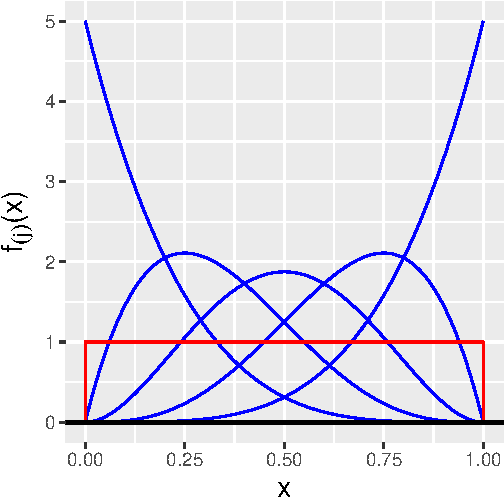
\includegraphics[keepaspectratio]{03-binomial_files/figure-latex/fig-betaunif-1.pdf}}

}

\caption{\label{fig-betaunif}The order statistic probability density
functions \(f_{(j)}(x)\) for, from left to right, \(j = 1\) through
\(j = 5\), for the situation in which \(n = 5\) iid data are drawn from
a Uniform(0,1) distribution (overlaid in red). Each pdf is itself a beta
distribution, with parameter values \(j\) and \(n-j+1\).}

\end{figure}%

\subsubsection{Order Statistic Distribution: Numeric
Calculation}\label{order-statistic-distribution-numeric-calculation}

\begin{quote}
Let's suppose that we sample \(n = 200\) data from a standard normal
distribution. Can we compute, e.g., \(f_{(70)}(x)\), for any given value
of \(x\)?
\end{quote}

\begin{quote}
Because we cannot easily determine in this case whether the
\(70^{\mathrm{th}}\) ordered datum is sampled according to some known,
named distribution, we will attack this via direct numeric computation.
Except\ldots the expression for \(f_{(j)}(x)\) contains factorial
functions, and evaluating factorial functions can lead to computational
overflow:
\end{quote}

\begin{Shaded}
\begin{Highlighting}[]
\FunctionTok{factorial}\NormalTok{(}\DecValTok{200}\NormalTok{)}
\end{Highlighting}
\end{Shaded}

\begin{verbatim}
[1] Inf
\end{verbatim}

\begin{quote}
Because of this, the ``safest'' approach is to compute the natural
logarithm of \(f_{(j)}\): \begin{align*}
\log f_{(j)} &= \log n! + \log f_X(x) + (j-1) \log F_X(x) + (n-j) \log [1 - F_X(x)]\\
&~~~~ - \log (j-1)! - \log (n-j)! \,.
\end{align*} In code, this would be expressed as
\end{quote}

\begin{Shaded}
\begin{Highlighting}[]
\NormalTok{n }\OtherTok{\textless{}{-}}   \DecValTok{200}
\NormalTok{j }\OtherTok{\textless{}{-}}    \DecValTok{70}
\NormalTok{x }\OtherTok{\textless{}{-}} \SpecialCharTok{{-}}\FloatTok{0.30}
\NormalTok{f.x }\OtherTok{\textless{}{-}} \FunctionTok{dnorm}\NormalTok{(x)}
\NormalTok{F.x }\OtherTok{\textless{}{-}} \FunctionTok{pnorm}\NormalTok{(x)}
\NormalTok{log.f.j }\OtherTok{\textless{}{-}} \FunctionTok{lfactorial}\NormalTok{(n) }\SpecialCharTok{+} \FunctionTok{log}\NormalTok{(f.x) }\SpecialCharTok{+}\NormalTok{ (j }\SpecialCharTok{{-}} \DecValTok{1}\NormalTok{) }\SpecialCharTok{*} \FunctionTok{log}\NormalTok{(F.x) }\SpecialCharTok{+}\NormalTok{ (n }\SpecialCharTok{{-}}\NormalTok{ j) }\SpecialCharTok{*} \FunctionTok{log}\NormalTok{(}\DecValTok{1} \SpecialCharTok{{-}}\NormalTok{ F.x) }\SpecialCharTok{{-}}
           \FunctionTok{lfactorial}\NormalTok{(j }\SpecialCharTok{{-}} \DecValTok{1}\NormalTok{) }\SpecialCharTok{{-}} \FunctionTok{lfactorial}\NormalTok{(n }\SpecialCharTok{{-}}\NormalTok{ j)}
\FunctionTok{exp}\NormalTok{(log.f.j)}
\end{Highlighting}
\end{Shaded}

\begin{verbatim}
[1] 2.654509
\end{verbatim}

\begin{quote}
One can repeat this calculation over, e.g., a sequence of \(x\) values
in order to visualize the probability density function.
\end{quote}

\begin{figure}

\centering{

\pandocbounded{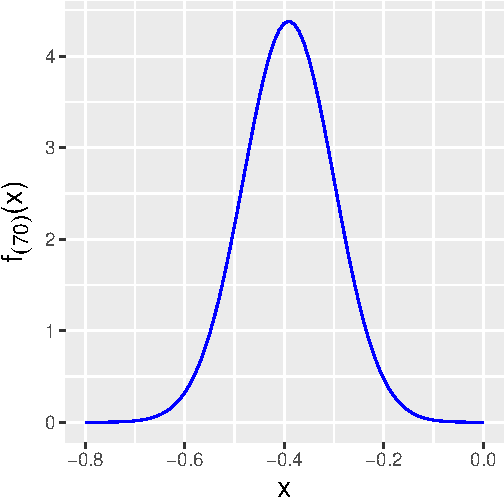
\includegraphics[keepaspectratio]{03-binomial_files/figure-latex/fig-pdford-1.pdf}}

}

\caption{\label{fig-pdford}The probability density function for the
\(j = 70^{\mathrm{th}}\) order statistic, given \(n = 200\) data sampled
according to a \(\mathcal{N}(\mu = 0,\sigma^2 = 1)\) distribution.}

\end{figure}%

\subsubsection{Discrete Order Statistic: Probability Mass
Function}\label{discrete-order-statistic-probability-mass-function}

\begin{quote}
Let's say that in an experiment, we flip a fair coin \(k = 10\) times
and record the number of heads as our random variable \(X\). We then
repeat this experiment \(n = 20\) times and arrange the 20 values
\(\{X_1,\ldots,X_{20}\}\) into ascending order. What is the probability
mass function for the \(17^{\mathrm{th}}\) ordered datum? We can
numerically determine the pmf using the code below. See
Figure~\ref{fig-pmford}.
\end{quote}

\begin{Shaded}
\begin{Highlighting}[]
\CommentTok{\# returns the cdf summation given above, for binomially distributed data}
\NormalTok{pbinom\_order }\OtherTok{\textless{}{-}} \ControlFlowTok{function}\NormalTok{(x, k, p, j, n)}
\NormalTok{\{}
\NormalTok{  i }\OtherTok{\textless{}{-}}\NormalTok{ j}\SpecialCharTok{:}\NormalTok{n}
  \FunctionTok{sum}\NormalTok{(}\FunctionTok{choose}\NormalTok{(n, i) }\SpecialCharTok{*}\NormalTok{ (}\FunctionTok{pbinom}\NormalTok{(x, k, p))}\SpecialCharTok{\^{}}\NormalTok{i }\SpecialCharTok{*}\NormalTok{ (}\DecValTok{1}\SpecialCharTok{{-}}\FunctionTok{pbinom}\NormalTok{(x, k, p))}\SpecialCharTok{\^{}}\NormalTok{(n }\SpecialCharTok{{-}}\NormalTok{ i))}
\NormalTok{\}}

\NormalTok{k }\OtherTok{\textless{}{-}} \DecValTok{10}
\NormalTok{p }\OtherTok{\textless{}{-}} \FloatTok{0.5}
\NormalTok{j }\OtherTok{\textless{}{-}} \DecValTok{17}
\NormalTok{n }\OtherTok{\textless{}{-}} \DecValTok{20}

\CommentTok{\# determine pmf for x = \{0, 1, ..., k\}}
\NormalTok{pmf\_order    }\OtherTok{\textless{}{-}} \FunctionTok{rep}\NormalTok{(}\ConstantTok{NA}\NormalTok{,k}\SpecialCharTok{+}\DecValTok{1}\NormalTok{)}
\NormalTok{pmf\_order[}\DecValTok{1}\NormalTok{] }\OtherTok{\textless{}{-}} \FunctionTok{pbinom\_order}\NormalTok{(}\DecValTok{0}\NormalTok{, k, p, j, n)}
\ControlFlowTok{for}\NormalTok{ ( ii }\ControlFlowTok{in} \DecValTok{2}\SpecialCharTok{:}\NormalTok{(k }\SpecialCharTok{+} \DecValTok{1}\NormalTok{) ) \{}
\NormalTok{  pmf\_order[ii] }\OtherTok{\textless{}{-}} \FunctionTok{pbinom\_order}\NormalTok{(ii }\SpecialCharTok{{-}} \DecValTok{1}\NormalTok{, k, p, j, n) }\SpecialCharTok{{-}} \FunctionTok{pbinom\_order}\NormalTok{(ii }\SpecialCharTok{{-}} \DecValTok{2}\NormalTok{, k, p, j, n)}
\NormalTok{\}}
\end{Highlighting}
\end{Shaded}

\begin{figure}

\centering{

\pandocbounded{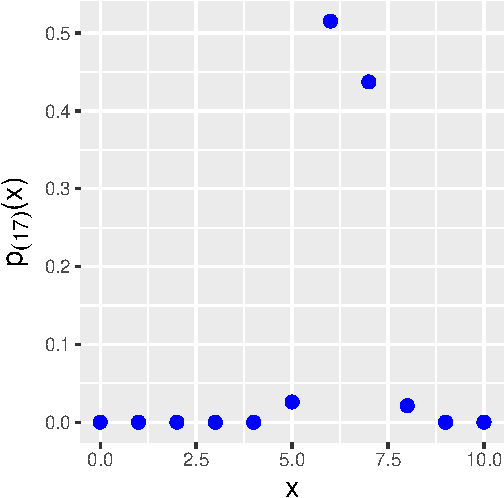
\includegraphics[keepaspectratio]{03-binomial_files/figure-latex/fig-pmford-1.pdf}}

}

\caption{\label{fig-pmford}The probability mass function for the
\(j = 17^{\mathrm{th}}\) order statistic, given \(n = 20\) data sampled
according to a Binom(\(k = 10,p = 0.5\)) distribution.}

\end{figure}%

\section{Point Estimation}\label{sec-chap3point}

What to take away from this section:

\begin{itemize}
\item
  Because maximum likelihood estimators for distribution parameters
  \(\theta\) are not always unbiased (although any bias goes away as the
  sample size increases), we introduce a second point estimator: the
  \emph{minimum variance unbiased estimator}, or \emph{MVUE}.
\item
  The derivation of an MVUE for \(\theta\) hinges upon the
  identification of a \emph{sufficient statistic} for \(\theta\).
\item
  Single-valued sufficient statistics exist for members of the
  \emph{exponential family of distributions}, which includes those
  distributions typically used in data analyses: the normal, the
  binomial, etc.
\item
  An MVUE does not possess the invariance property, nor is there a
  guarantee that it converges in distribution to a normal random
  variable.
\end{itemize}

For previous material on point estimation, see
Section~\ref{sec-chap2point}.

In Section~\ref{sec-chap1point} and Section~\ref{sec-chap2point}, we
introduce a number of concepts related to point estimation, the act of
using statistics to make inferences about a population parameter
\(\theta\). We\ldots{}

\begin{itemize}
\tightlist
\item
  assess point estimators using the metrics of bias, variance,
  mean-squared error, and consistency;
\item
  utilize the Fisher information metric to determine the lower bound on
  the variance for unbiased estimators (the Cramer-Rao Lower Bound, or
  CRLB); and
\item
  define estimators via the maximum likelihood algorithm, which
  generates estimators that are at least asymptotically unbiased and at
  least asymptotically reach the CRLB, and which converge in
  distribution to normal random variables.
\end{itemize}

We will review these concepts in the context of estimating population
quantities for binomial distributions below, in the body of the text and
in examples. For now\ldots{}

\smallskip\hrule

\begin{quote}
\textbf{Recall}: \emph{the bias of an estimator is the difference
between the average value of the estimates it generates and the true
parameter value. If \(E[\hat{\theta}-\theta] = 0\), then the estimator
\(\hat{\theta}\) is said to be unbiased.}
\end{quote}

\smallskip\hrule

\begin{quote}
\textbf{Recall}: \emph{the value of \(\theta\) that maximizes the
likelihood function is the maximum likelihood estimate, or MLE, for
\(\theta\). The maximum is found by taking the (partial) derivative of
the (log-)likelihood function with respect to \(\theta\), setting the
result to zero, and solving for \(\theta\). That solution is the maximum
likelihood estimate \(\hat{\theta}_{MLE}\). Also recall the invariance
property of the MLE: if \(\hat{\theta}_{MLE}\) is the MLE for
\(\theta\), then \(g(\hat{\theta}_{MLE})\) is the MLE for
\(g(\theta)\).}
\end{quote}

\smallskip\hrule

\subsection{Sufficient Statistics}\label{sec-chap3sufficient}

A \emph{sufficient statistic} for a parameter \(\theta\) captures all
information about \(\theta\) contained in the sample. The sufficiency
principle holds that if, e.g., \(Y\) is a sufficient statistic for
\(\theta\), and we collect two datasets \(\mathbf{U}\) and
\(\mathbf{V}\) such that \(Y(\mathbf{U}) = Y(\mathbf{V})\), then the
inferences we make about \(\theta\) given that we observe \(\mathbf{U}\)
will be exactly the same as those we would make if we were to observe
\(\mathbf{V}\). Using any statistic beyond a sufficient statistic will
not lead to improved inferences about \(\theta\). This means that, for
instance, combining \(\bar{X}\) (a sufficient statistic for the normal
mean \(\mu\) when the variance is known) with, say, the sample median
will not reduce the length of confidence intervals for \(\mu\) or change
the power of hypothesis tests about \(\mu\), relative to what we would
find using \(\bar{X}\) alone. Note that utilizing the sufficiency
principle is but one way by which statisticians can attempt \emph{data
reduction} prior to inference; two others, which are beyond the scope of
this book, are the likelihood and equivalence principles. For a deeper
treatment of sufficiency and data reduction than we provide here, the
interested reader should consult Chapter 6 of Casella and Berger (2002).

A statistic \(Y(\mathbf{X})\) is a sufficient statistic for \(\theta\)
if the ratio \begin{align*}
\frac{f_X(\mathbf{x} \vert \theta)}{f_Y(y \vert \theta)} \overset{iid}{\rightarrow} \frac{\prod_{i=1}^n f_X(x_i \vert \theta)}{f_Y(y \vert \theta)} \,,
\end{align*} where \(f_Y(y \vert \theta)\) is the probability density
function of the sampling distribution for \(Y\), is constant as a
function of \(\theta\). We note that by this definition, \(\mathbf{X}\)
itself comprises a sufficient statistic for \(\theta\), as does the full
set of order statistics \(\{X_{(1)},\ldots,X_{(n)}\}\). The relevant
questions are: can we define a sufficient statistic that actually
reduces the data? And if so, how can we identify it?

Let's answer the second question first. The simplest way by which to
identify a sufficient statistic is to write down the likelihood function
and then to factorize it into two separate functions, one of which
depends \emph{only} on the observed data and the other of which depends
on both the observed data and the parameter of interest: \[
\mathcal{L}(\theta \vert \mathbf{x}) = h(\mathbf{x}) \cdot g(\mathbf{x},\theta) \,.
\] This is the so-called \emph{factorization criterion}. In the
expression \(g(\mathbf{x},\theta)\), the data will appear within, e.g.,
a summation (e.g., \(\sum_{i=1}^n x_i\)) or a product (e.g.,
\(\prod_{i=1}^n x_i\)), and we would identify that summation or product
as a sufficient statistic for \(\theta\). For instance, for the binomial
distribution, the factorized likelihood (given \(n\) iid data) is \[
\mathcal{L}(p \vert \mathbf{x}) = \prod_{i=1}^n \binom{k}{x_i} p^{x_i} (1-p)^{k-x_i} = \underbrace{\left[ \prod_{i=1}^n \binom{k}{x_i} \right]}_{h(\mathbf{x})} \underbrace{p^{\sum_{i=1}^n x_i} (1-p)^{nk-\sum_{i=1}^n x_i}}_{g(\sum_{i=1}^n x_i,p)} \,.
\] By inspecting the function \(g(\mathbf{x},p)\), we immediately
determine that \(Y = X_+ = \sum_{i=1}^n X_i\) is a sufficient statistic
for \(p\). We say that \(X_+\) is ``a'' sufficient statistic because
sufficient statistics are not unique: \emph{any one-to-one function of a
sufficient statistic is also a sufficient statistic}. For instance, if
\(X_+\) is a sufficient statistic for \(\theta\), then so is
\(\bar{X}\), etc.

Now we return to the first question above: can we define a sufficient
statistic that actually reduces the data? The answer is ``not always.''
In fact, across all possible distributions, it is relatively rare that
we can do this. The Pitman-Koopman-Darmois theorem holds that, among
families of distributions that do not have domain-specifying parameters,
only members of the exponential family of distributions have sufficient
statistics whose dimension does not increase as the sample size
increases. (This theorem motivates, in large part, why we introduce the
exponential family in Section~\ref{sec-chap2exponential}.)

\smallskip\hrule

\begin{quote}
\textbf{Recall:} \emph{the exponential family of distributions is the
set of distributions whose probability mass or density functions can be
expressed as} \[
h(x) \exp\left[\left(\sum_{i=1}^p \eta_i(\boldsymbol{\theta}) T_i(x)\right) - A(\boldsymbol{\theta})\right] \,,
\] \emph{where \(\boldsymbol{\theta}\) is a vector of parameters (e.g.,
\(\boldsymbol{\theta} = \{\mu,\sigma^2\}\) for a normal distribution).
Note that none of the parameters can be a domain-specifying parameter.}
\end{quote}

\smallskip\hrule

Let's assume that we are dealing with distributions that have just one
free parameter \(\theta\), like the binomial distribution. Then the
expression above simplifies to \begin{align*}
h(x) \exp\left[ \eta(\theta) T(x) - A(\theta) \right] \,,
\end{align*} where \(T(x)\) is a sufficient statistic. For a single
binomially distributed datum, \(T(X) = X\). If on the other hand we
collect \(n\) iid data, then a sufficient statistic is
\(T(\mathbf{X}) = \sum_{i=1}^n X_i\), and as we can see it is still a
single number\(-\)i.e., it has a dimension of one\(-\)regardless of the
value of \(n\). Now, restricting ourselves to exponential family
distributions in inferential situations would appear to limit the
practical utility of the sufficiency principle\ldots except it is the
case that \emph{many} (if not \emph{most}) of the distributions that we
typically utilize in inference are indeed exponential-family
distributions, including all the ones that we focus on in chapters
\hyperref[sec-chap2]{2}-\hyperref[sec-chap4]{4} of this book.

(We note here for completeness that once we identify a sufficient
statistic, we are technically required to demonstrate that it is both
\emph{minimally sufficient} and \emph{complete}, as it needs to be both
so that we can use it to, e.g., determine the minimum variance unbiased
estimator. It suffices to say here that the sufficient statistics that
we identify for exponential family distributions via likelihood
factorization are minimally sufficient and complete. See
Section~\ref{sec-chap7suffminimal} and
Section~\ref{sec-chap7suffcomplete} for more details on minimal
sufficiency and completeness, respectively.)

\subsection{Minimum Variance Unbiased Estimation}\label{sec-chap3mvue}

Given the concept of sufficiency, we can now introduce another means by
which to define an estimator. The \emph{minimum variance unbiased
estimator} (or \emph{MVUE}) is the one that has the smallest variance
among all unbiased estimators of \(\theta\). The reader's first thought
might be ``well, why didn't we use this estimator in the first
place\ldots after all, the MLE is not guaranteed to yield an unbiased
estimator, so why have we put off discussing the MVUE?'' The primary
reasons are that MVUEs are sometimes not definable (i.e., we can reach
insurmountable computational roadblocks when trying to derive them), and
unlike MLEs, they do not exhibit the invariance property. (For instance,
if \(\hat{\theta}_{MLE} = \bar{X}\), then
\(\hat{\theta^2}_{MLE} = \bar{X}^2\), but if
\(\hat{\theta}_{MVUE} = \bar{X}\), it is not necessarily the case that
\(\hat{\theta^2}_{MVUE} = \bar{X}^2\).) \emph{However, we should always
at least try to define the MVUE, because if we can, it will be at least
equal the performance of, if not perform better than, the MLE, in terms
of mean-squared error.}

There are two steps to carry out when deriving the MVUE:

\begin{enumerate}
\def\labelenumi{\arabic{enumi}.}
\tightlist
\item
  determining a sufficient statistic for \(\theta\); and
\item
  correcting any bias that is observed when we utilize that sufficient
  statistic as our initial estimator.
\end{enumerate}

If \(Y\) is a sufficient statistic for \(\theta\), and there is a
function \(h(Y)\) that is an unbiased estimator for \(\theta\) and that
depends on the data only through \(Y\), then \(h(Y)\) is the MVUE for
\(\theta\). (A reader who is interested in the underlying theory should
reference the Lehmann-Scheff\textquotesingle e theorem.) Recall from
above that one-to-one functions of sufficient statistics are themselves
sufficient statistics, hence \(h(Y)\) is also going to be sufficient for
\(\theta\). Here, given \(Y = \sum_{i=1}^n X_i\), we need to find a
function \(h(\cdot)\) such that \(E[h(Y)] = p\). In
Section~\ref{sec-chap3linear}, we determined that the distribution for
the sum of iid binomial random variables is Binomial(\(nk\),\(p\)), and
thus we know that this distribution has expected value \(nkp\). Thus \[
E\left[Y\right] = nkp ~\implies~ E\left[\frac{Y}{nk}\right] = p ~\implies~ h(Y) = \frac{Y}{nk} = \frac{\bar{X}}{k} 
\] is the MVUE for \(p\). The variance of \(\hat{p}\) is \[
V[\hat{p}] = V\left[\frac{\bar{X}}{k}\right] = \frac{1}{k^2}V[\bar{X}] = \frac{1}{k^2} \frac{V[X]}{n} = \frac{1}{k^2}\frac{kp(1-p)}{n} = \frac{p(1-p)}{nk} \,.
\] We know that this variance abides by the restriction \[
V[\hat{p}] \geq \frac{1}{nI(p)} = -\frac{1}{nE\left[\frac{d^2}{dp^2} \log p_X(X \vert p) \right]} \,.
\] But is it equivalent to the lower bound for unbiased estimators, the
CRLB? (Note that in particular situations, the MVUE \emph{may} have a
variance larger than the CRLB; when this is the case, unbiased
estimators that achieve the CRLB simply do not exist.) For the binomial
distribution, \begin{align*}
p_{X}(x) &= \binom{k}{x} p^{x} (1-p)^{k-x} \\
\log p_{X}(x) &= \log \binom{k}{x} + x \log p + (k-x) \log (1-p) \\
\frac{d}{dp} \log p_{X}(x) &= 0 + \frac{x}{p} - \frac{k-x}{(1-p)} \\
\frac{d^2}{dp^2} \log p_{X}(x) &= -\frac{x}{p^2} - \frac{k-x}{(1-p)^2} \\
E\left[\frac{d^2}{dp^2} \log p_{X}(X)\right] &= -\frac{1}{p^2}E[X] - \frac{1}{(1-p)^2}E[k-X] \\
&= -\frac{kp}{p^2}-\frac{k-kp}{(1-p)^2} \\
&= -\frac{k}{p}-\frac{k}{1-p} = -\frac{k}{p(1-p)} \,.
\end{align*} The lower bound on the variance is thus \(p(1-p)/(nk)\),
and so the MVUE \emph{does} achieve the CRLB. \emph{We cannot define a
better unbiased estimator for \(p\) than \(\bar{X}/k\).}

For more on point estimation, go to Section~\ref{sec-chap4point}.

\subsection{Examples}\label{examples-31}

\subsubsection{The MLE for the Binomial Success
Probability}\label{the-mle-for-the-binomial-success-probability}

\smallskip\hrule

\begin{quote}
\textbf{Recall}: \emph{the value of \(\theta\) that maximizes the
likelihood function is the maximum likelihood estimate, or MLE, for
\(\theta\). The maximum is found by taking the (partial) derivative of
the (log-)likelihood function with respect to \(\theta\), setting the
result to zero, and solving for \(\theta\). That solution is the maximum
likelihood estimate \(\hat{\theta}_{MLE}\).}
\end{quote}

\smallskip\hrule

\begin{quote}
Above, we determined that the likelihood function for \(n\) iid binomial
random variables \(\{X_1,\ldots,X_n\}\) is \[
\mathcal{L}(p \vert \mathbf{x}) = \left[\prod_{i=1}^n \binom{k}{x_i} \right] p^{\sum_{i=1}^n x_i} (1-p)^{nk-\sum_{i=1}^n x_i} \,.
\] Recall that the value \(\hat{p}_{MLE}\) that maximizes
\(\mathcal{L}(p \vert \mathbf{x})\) also maximizes
\(\ell(p \vert \mathbf{x}) = \log \mathcal{L}(p \vert \mathbf{x})\),
which is considerably easier to work with: \begin{align*}
\ell(p \vert \mathbf{x}) &= \left(\sum_{i=1}^n x_i\right) \log p + \left(nk - \sum_{i=1}^n x_i\right) \log (1-p) \\
\ell'(p \vert \mathbf{x}) &= \frac{d}{dp} \ell(p \vert \mathbf{x}) = \frac{1}{p} \sum_{i=1}^n x_i - \frac{1}{1-p} \left(nk - \sum_{i=1}^n x_i\right) \,.
\end{align*} (Here, we drop the binomial coefficient, which does not
depend on \(p\) and thus differentiates to zero.) After setting
\(\ell'(p \vert \mathbf{x})\) to zero and rearranging terms, we find
that \[
p = \frac{1}{nk}\sum_{i=1}^n x_i ~\implies~ \hat{p}_{MLE} = \frac{\bar{X}}{k} \,.
\] The MLE matches the MVUE, thus we know that the MLE is unbiased and
we know that it achieves the CRLB.
\end{quote}

\smallskip\hrule

\begin{quote}
\textbf{Recall}: \emph{the bias of an estimator is the difference
between the average value of the estimates it generates and the true
parameter value. If \(E[\hat{\theta}-\theta] = 0\), then the estimator
\(\hat{\theta}\) is said to be unbiased.}
\end{quote}

\smallskip\hrule

\begin{quote}
\textbf{Recall}: \emph{the Cramer-Rao Lower Bound (or CRLB) is the lower
bound on the variance of any unbiased estimator. If an unbiased
estimator achieves the CRLB, it is the MVUE\ldots but it can be the case
that the MVUE does not achieve the CRLB. For a discrete distribution,
the CRLB is given by} \[
V_{\mathrm{CRLB}}[\hat{\theta}] = -\left(nE\left[\frac{d^2}{d\theta^2} \log p_X(X \vert p) \right]\right)^{-1} = \frac{1}{nI(\theta)}
\] \emph{where \(I(\theta)\) is the Fisher information:} \[
I(\theta) = -E\left[ \frac{\partial^2}{\partial \theta^2} \log f_X(x \vert \theta) \right] \,.
\]
\end{quote}

\smallskip\hrule

\begin{quote}
A useful property of MLEs is the invariance property, which holds that
the MLE for a function of \(\theta\) is given by applying the same
function to the MLE itself. Thus
\end{quote}

\begin{quote}
\begin{itemize}
\tightlist
\item
  the MLE for the population mean \(E[X] = \mu = kp\) is
  \(\hat{\mu}_{MLE} = \bar{X}\); and
\item
  the MLE for the population variance \(V[X] = \sigma^2 = kp(1-p)\) is
  \(\widehat{\sigma^2}_{MLE} = \bar{X}(1-\bar{X}/k)\).
\end{itemize}
\end{quote}

\begin{quote}
Last, note \(\hat{p}_{MLE}\) is a consistent estimator (like all MLEs)
and that asymptotically, it converges in distribution to a normal random
variable (like all MLEs): \[
\hat{p}_{MLE} \overset{d}{\rightarrow} Y \sim \mathcal{N}\left(p,\frac{1}{nI(p)} = \frac{p(1-p)}{nk}\right) \,.
\]
\end{quote}

\smallskip\hrule

\begin{quote}
\textbf{Recall}: \emph{an estimator is consistent if its mean-squared
error, \(B[\hat{\theta}]^2 + V[\hat{\theta}]\), goes to zero as the
sample size \(n\) goes to infinity.}
\end{quote}

\smallskip\hrule

\subsubsection{Normal Distribution: Sufficient
Statistics}\label{normal-distribution-sufficient-statistics}

\begin{quote}
If we have \(n\) iid data drawn from a normal distribution with unknown
mean \(\mu\) and unknown variance \(\sigma^2\), then the factorized
likelihood is \begin{align*}
&\mathcal{L}(\mu,\sigma^2 \vert \mathbf{x}) \\
= ~ &\underbrace{(2 \pi \sigma^2)^{-n/2} \exp\left(-\frac{1}{2\sigma^2}\sum_{i=1}^n x_i^2\right)\exp\left(\frac{\mu}{\sigma^2}\sum_{i=1}^n x_i\right)\exp\left(-\frac{n\mu^2}{2\sigma^2}\right)}_{g(\sum x_i^2, \sum x_i,\mu,\sigma)} \cdot \underbrace{1}_{h(\mathbf{x})} \,.
\end{align*} Here, we identify \(\sum x_i^2\) and \(\sum x_i\) as
\emph{joint} sufficient statistics: we need two pieces of information to
jointly estimate \(\mu\) and \(\sigma^2\). (To be clear: it is not
necessarily the case that one of the parameters matches to one of the
statistics\ldots rather, the two statistics are jointly sufficient for
estimation.) We thus cannot proceed further to define an MVUE for
\(\mu\) or for \(\sigma^2\), without knowing the joint bivariate
probability density function for \(Y_1 = \sum_{i=1}^n X_i^2\) and
\(Y_2 = \sum_{i=1}^n X_i\).
\end{quote}

\begin{quote}
(Note that we \emph{can} proceed if we happen to know either \(\mu\) or
\(\sigma^2\); if one of these values is fixed, then there will only be
one sufficient statistic and we can determine the MVUE for the other,
freely varying parameter.)
\end{quote}

\subsubsection{Sufficiency: When We Cannot Reduce
Data}\label{sufficiency-when-we-cannot-reduce-data}

\begin{quote}
As stated above, it is often impossible to reduce data to, e.g., a
single-number summary. The following examples, utilizing distributions
that are \emph{not} exponential-family distributions, illustrate this.
\end{quote}

\begin{quote}
\begin{enumerate}
\def\labelenumi{\arabic{enumi}.}
\tightlist
\item
  A Laplace distribution with scale parameter 1 has the probability
  density function \begin{align*}
  f_X(x \vert \theta) &= \frac12 e^{-\vert x - \theta \vert} \,,
  \end{align*} where \(x \in (-\infty,\infty)\) and
  \(\theta \in (-\infty,\infty)\). If we observe \(n\) iid data, then
  likelihood factorization yields \begin{align*}
  \mathcal{L}(\theta \vert \mathbf{x}) = \frac{1}{2^n} e^{-\sum_{i=1}^n \vert x_i - \theta \vert} \,.
  \end{align*} \(Y = \sum_{i=1}^n \vert X_i - \theta \vert\) is not a
  sufficient statistic as it contains the (unknown) parameter: a
  sufficient statistic for \(\theta\) cannot contain \(\theta\) itself!
  We cannot isolate a function of \(\mathbf{X}\) alone, and thus no data
  reduction is possible.
\end{enumerate}
\end{quote}

\begin{quote}
\begin{enumerate}
\def\labelenumi{\arabic{enumi}.}
\setcounter{enumi}{1}
\tightlist
\item
  A Cauchy distribution with scale parameter 1 has the probability
  density function \begin{align*}
  f_X(x \vert \theta) = \frac{1}{\pi (x-\theta)^2} \,,
  \end{align*} where \(x \in (-\infty,\infty)\) and
  \(\theta \in (-\infty,\infty)\). If we observe \(n\) iid data, then
  likelihood factorization yields \begin{align*}
  \mathcal{L}(\theta \vert \mathbf{x}) = \frac{1}{\pi^n} \frac{1}{\prod_{i=1}^n (x_i-\theta)^2} \,.
  \end{align*} Again, we cannot isolate a function of the \(X_i\)'s
  alone: no data reduction is possible.
\end{enumerate}
\end{quote}

\subsubsection{Exponential Distribution: MVUE for Population
Mean}\label{exponential-distribution-mvue-for-population-mean}

\begin{quote}
The exponential distribution is \[
f_X(x) = \frac{1}{\theta} \exp\left(-\frac{x}{\theta}\right) \,,
\] where \(x \geq 0\) and \(\theta > 0\), and where \(E[X] = \theta\)
and \(V[X] = \theta^2\). Let's assume that we have \(n\) iid data drawn
from this distribution. Can we define the MVUE for \(\theta\)? For
\(\theta^2\)?
\end{quote}

\begin{quote}
The likelihood function is \[
\mathcal{L}(\theta \vert \mathbf{x}) = \prod_{i=1}^n f_X(x_i \vert \theta) = \frac{1}{\theta^n}\exp\left(-\frac{1}{\theta}\sum_{i=1}^n x_i \right) = h(\mathbf{x}) \cdot g(\theta,\mathbf{x}) \,.
\] Here, there are no terms that are functions of only the data, so
\(h(\mathbf{x}) = 1\) and a sufficient statistic is
\(Y = \sum_{i=1}^n X_i\). We compute the expected value of \(Y\): \[
E[Y] = E\left[\sum_{i=1}^n X_i\right] = \sum_{i=1}^n E[X_i] = \sum_{i=1}^n \theta = n\theta \,.
\] The expected value of \(Y\) is not \(\theta\), so \(Y\) is not
unbiased\ldots but we can see immediately that \(E[Y/n] = \theta\), so
that \(Y/n\) is unbiased. Thus the MVUE for \(\theta\) is thus
\(\hat{\theta}_{MVUE} = Y/n = \bar{X}\).
\end{quote}

\begin{quote}
Note that the MVUE does not possess the invariance property\ldots it is
not necessarily the case that \(\hat{\theta^2}_{MVUE} = \bar{X}^2\).
\end{quote}

\begin{quote}
Let's propose a function of \(Y\) and see if we can use that to define
\(\hat{\theta^2}_{MVUE}\): \(h(Y) = Y^2/n^2 = \bar{X}^2\). (To be clear,
we are simply proposing a function and seeing if it helps us define what
we are looking for. It might not. If not, we can try again with another
function of \(Y\).) Utilizing what we know about the sample mean, we can
write down that \[
E[\bar{X}^2] = V[\bar{X}] + (E[\bar{X}])^2 = \frac{V[X]}{n} + (E[X])^2 = \frac{\theta^2}{n}+\theta^2 = \theta^2\left(\frac{1}{n} + 1\right) \,.
\] So \(\bar{X}^2\) itself is \emph{not} an unbiased estimator of
\(\theta^2\)\ldots but we can see that \(\bar{X}^2/(1/n+1)\) is. Hence
\[
\hat{\theta^2}_{MVUE} = \frac{\bar{X}^2}{\left(\frac{1}{n}+1\right)} \,.
\]
\end{quote}

\subsubsection{Geometric Distribution: MVUE for Number of
Failures}\label{geometric-distribution-mvue-for-number-of-failures}

\begin{quote}
Recall that the geometric distribution is a negative binomial
distribution with \(s = 1\): \begin{align*}
p_X(x) = \binom{x + s - 1}{x} p^s (1-p)^x ~ \rightarrow ~ p(1-p)^x \,,
\end{align*} where \(p \in (0,1]\) and where \(E[X] = (1-p)/p\) and
\(V[X] = (1-p)/p^2\). Let's assume that we sample \(n\) iid data from
this distribution. Can we define the MVUE for \(p\)? For \(1/p\)?
\end{quote}

\begin{quote}
The likelihood function is \begin{align*}
\mathcal{L}(p \vert \mathbf{x}) = \prod_{i=1}^n p_X(x_i \vert p) = p^n (1-p)^{\sum_{i=1}^n x_i} = 1 \cdot g(p,\mathbf{x}) \,.
\end{align*} We identify a sufficient statistic as
\(Y = \sum_{i=1}^n X_i\); the expected value of \(Y\) is \begin{align*}
E[Y] = E\left[\sum_{i=1}^n X_i\right] = \sum_{i=1}^n E[X_i] = \sum_{i=1}^n \frac{1-p}{p} = n\left(\frac{1}{p}-1\right) \,.
\end{align*} We cannot ``debias'' this expression to find the MVUE for
\(p\), but we can do it to find the MVUE for the number of failures:
\begin{align*}
E\left[\frac{Y}{n}\right] = \frac{1}{p} - 1\,.
\end{align*} As there is no invariance property for the MVUE, we cannot
use this expression to write down the MVUE for \(p\) itself.
\end{quote}

\subsubsection{Order Statistics: Distribution-Free Percentile
Estimate}\label{order-statistics-distribution-free-percentile-estimate}

\begin{quote}
Let's suppose a setting that we have yet to explore in this book: we are
given \(n\) iid data \(\mathbf{X} = \{X_1,\ldots,X_n\}\) sampled
according to an unknown continuous distribution. This is the
\emph{distribution-free} setting, and in such a setting our
opportunities for inference are limited: we can only make statements
about population percentiles such as the population median (aka the
distribution's \(50^{\mathrm{th}}\) percentile), unless we make further
assumptions. (For instance, if we assume that the underlying
distribution has a symmetric probability density function, then we can
make statements about the population mean.) For clarity, a
``percentile'\,' \(\chi_q\) denotes the probability of sampling a random
variable with a value less than or equal to \(\chi_q\), i.e.,
\(P(X \leq \chi_q)\).
\end{quote}

\begin{quote}
Let's say we are given the following data:
\end{quote}

\begin{verbatim}
 [1] 0.275 0.430 0.687 0.717 1.252 1.275 1.386 2.262 3.327 3.447 4.127
\end{verbatim}

\begin{quote}
How would we specify a point estimate for, e.g., the underlying
distribution's \(75^{\mathrm{th}}\) percentile (\(\chi_{0.75}\))?
\end{quote}

\begin{quote}
We will state a key takeaway from this example now: \emph{there is no
unique algorithm for estimating a percentile!} To underscore this point,
we note that \texttt{R}'s \texttt{quantile()} function allows us to
utilize any one of \emph{nine} quantile-estimating algorithms (as
specified by the argument \texttt{type}). We will concentrate here on
that function's default algorithm (Type 7).
\end{quote}

\begin{quote}
Let the percentile be \(100q\); thus, here, \(q = 0.75\). The sample
percentile for each order statistic is \(q_{(j)} = (j-1)/(n-1)\), thus
\end{quote}

{\def\LTcaptype{none} % do not increment counter
\begin{longtable}[]{@{}
  >{\centering\arraybackslash}p{(\linewidth - 2\tabcolsep) * \real{0.2500}}
  >{\centering\arraybackslash}p{(\linewidth - 2\tabcolsep) * \real{0.2500}}@{}}
\toprule\noalign{}
\begin{minipage}[b]{\linewidth}\centering
q
\end{minipage} & \begin{minipage}[b]{\linewidth}\centering
x
\end{minipage} \\
\midrule\noalign{}
\endhead
\bottomrule\noalign{}
\endlastfoot
0.0 & 0.275 \\
0.1 & 0.430 \\
0.2 & 0.687 \\
0.3 & 0.717 \\
0.4 & 1.252 \\
0.5 & 1.275 \\
0.6 & 1.386 \\
0.7 & 2.262 \\
0.8 & 3.327 \\
0.9 & 3.447 \\
1.0 & 4.127 \\
\end{longtable}
}

\begin{quote}
To find the \(75^{\mathrm{th}}\) percentile, we would linearly
interpolate between 2.262 (for \(q = 0.7\)) and 3.327 (for \(q = 0.8\)):
this yields 2.7945, which matches the output from \texttt{quantile()}:
\end{quote}

\begin{Shaded}
\begin{Highlighting}[]
\FunctionTok{quantile}\NormalTok{(X, }\AttributeTok{probs =} \FunctionTok{c}\NormalTok{(}\FloatTok{0.75}\NormalTok{))}
\end{Highlighting}
\end{Shaded}

\begin{verbatim}
   75% 
2.7945 
\end{verbatim}

\begin{quote}
We note that this quantile estimate will be biased (but asymptotically
unbiased), since the range of data mapped to percentiles (0.275 - 4.127)
will not match the distribution's domain except in the limit of infinite
data. Also, the reader should immediately see how extending this
algorithm to discrete order statistics would be problematic, as the
point estimate will not necessarily match any of values in the
distribution's domain. We encourage those readers who want to learn more
about estimating percentiles for discrete distributions to explore the
algorithms dubbed Type 1 - Type 3 in the documentation for
\texttt{quantile()}, and the references given at the end of that
documentation.
\end{quote}

\section{Confidence Intervals}\label{sec-chap3confidence}

What to take away from this section:

\begin{itemize}
\item
  Given \(n\) iid data sampled according to a normal distribution, we
  can utilize numerical root-finding frameworks to construct
  \(100(1-\alpha)\)-percent confidence intervals for the binomial
  success proportion \(p\), as well as the parameters of related
  discrete distributions like the negative binomial.
\item
  Since the sampling distributions are discrete distributions, we must
  sometimes make \emph{discreteness corrections} (such as subtracting 1
  from the observed statistic value) when calling numerical root-finding
  functions.
\item
  And because the sampling distributions are discrete distributions, the
  interval coverage (i.e., the proportion of intervals that overlap the
  true value of \(\theta\)) will be \(\geq 1-\alpha\), with the equality
  achieved as the sample size (or, e.g., the number of trials) goes to
  infinity.
\end{itemize}

For previous material on confidence intervals, see
Section~\ref{sec-chap2confidence}.

\smallskip\hrule

\begin{quote}
\textbf{Recall:} \emph{a confidence interval is a random interval
\([\hat{\theta}_L,\hat{\theta}_U]\) that, when we work with continuous
sampling distributions, overlaps (or covers) the true value \(\theta\)
with probability} \[
P\left( \hat{\theta}_L \leq \theta \leq \hat{\theta}_U \right) = 1 - \alpha \,,
\] \emph{where \(1 - \alpha\) is the confidence coefficient. Note that
this is a long-term probabilistic statement that is not to be applied to
any one numerically evaluated interval: an evaluated interval either
overlaps the true value, or it does not (and thus we cannot say there is
a \(100(1-\alpha)\)-percent chance that \(\theta\) lies within the
interval). We determine \(\hat{\theta}\) by solving the following
equation:} \[
F_Y(y_{\mathrm{obs}} \vert \theta) - q = 0 \,,
\] \emph{where \(F_Y(\cdot)\) is the cumulative distribution function
for the statistic \(Y\), \(y_{\mathrm{obs}}\) is the observed value of
the statistic, and \(q\) is an appropriate quantile value that is
determined using the confidence interval reference table introduced in
Section~\ref{sec-chap1confref}.}
\end{quote}

\smallskip\hrule

A concept that we have not explicitly discussed yet is the ``duality''
between confidence intervals and hypothesis tests: as they are
mathematically related, one can, in theory, ``invert'' hypothesis tests
to derive confidence intervals and vice-versa. We illustrate this
duality in Figure~\ref{fig-contcdfci}, in which we assume that the
distribution from which we are to sample data is a normal distribution
with mean \(\mu\) and \emph{known} variance \(\sigma^2\). The parallel
green lines in the figure represent lower and upper rejection region
boundaries as a function of (the null hypothesis value) \(\mu\). Let's
say that we pick a specific value of \(\mu\), say \(\mu = \mu_o = 1\),
and draw a vertical line at that coordinate. The part of that line that
lies between the parallel green lines (indicated in solid red) indicates
the range of observed statistic values \(y_{\mathrm{obs}}\) for which we
would \emph{fail to reject} the null, and the parts above and below the
parallel lines (shown in dashed red) would indicate \(y_{\mathrm{obs}}\)
values for which we would \emph{reject} the null. (These are the
acceptance and rejection regions, respectively; ``acceptance region'' is
a term that we have not used up until now, but it simply denotes the
range of statistic values for which we would \emph{fail} to reject a
null hypothesis, when it is indeed correct.) Confidence intervals, on
the other hand, are ranges of values of \(\mu\) for which a given value
of \(y_{\mathrm{obs}}\) lies in the acceptance region. (For instance,
the dashed horizontal blue line in the figure shows the range of values
associated with a two-sided confidence interval for \(\mu\) given
\(y_{\mathrm{obs}} = 0.5\).) We can see that for a given value of
\(\mu\), if we were to sample a value of \(y_{\mathrm{obs}}\) between
the two green lines (with probability \(1-\alpha\)), then the associated
confidence interval will overlap \(\mu\), and if we sample a value of
\(y_{\mathrm{obs}}\) outside the green lines (with probability
\(\alpha\)), the confidence interval will \emph{not} overlap \(\mu\).
The confidence interval coverage is thus exactly \(100(1-\alpha)\)
percent.

\begin{figure}

\centering{

\pandocbounded{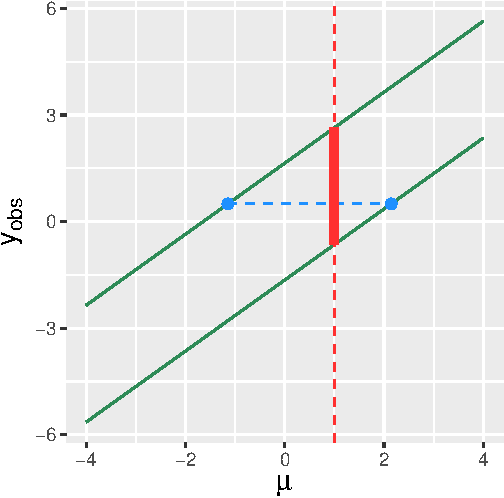
\includegraphics[keepaspectratio]{03-binomial_files/figure-latex/fig-contcdfci-1.pdf}}

}

\caption{\label{fig-contcdfci}An illustration of the relationship
between hypothesis testing and confidence interval estimation for a
continuous sampling distribution (here, a normal distribution with known
variance). The two parallel green lines define rejection-region
boundaries for a two-sided test with null hypothesis parameter value
\(\mu\). Assume \(\mu = 1\): the dashed red lines indicate the values of
\(y_{\mathrm{obs}}\) in the rejection region, while the solid red line
indicates the values of \(y_{\mathrm{obs}}\) in the acceptance region
(where we fail to reject the null). The horizontal dashed blue line
shows the confidence interval constructed for a given value of
\(y_{\mathrm{obs}}\). Given \(\mu\), the probability of sampling a
statistic in the acceptance region is exactly \(1-\alpha\), and thus the
coverage of confidence intervals will also be exactly \(1-\alpha\).}

\end{figure}%

\subsection{Working With Discrete Sampling
Distributions}\label{sec-chap3confdisc}

When we work with discrete sampling distributions, the overall picture
is similar, but we sometimes need to make what we will dub
``discreteness corrections'' so that the codes we use generate the
correct results. Figure~\ref{fig-disccicover} is an analogue to
Figure~\ref{fig-contcdfci} in which we illustrate the relationship
between confidence intervals and hypothesis tests for a situation in
which we conduct \(k = 10\) binomial trials. Because the statistic is
discretely valued, the acceptance-region boundaries are step functions,
but this is not the only change introduced with discrete distributions:

\begin{enumerate}
\def\labelenumi{\arabic{enumi}.}
\item
  In the continuous case, the probability of sampling a datum that lies
  within the acceptance region for a given value of \(\theta\) is
  exactly \(1 - \alpha\). In the discrete case, the probability is
  \(\geq 1 - \alpha\). (And it will rarely, if ever, be the case that
  the probability masses within the acceptance region will sum to
  exactly \(1 - \alpha\)\ldots although the sum will converge towards
  \(1 - \alpha\) as \(nk \rightarrow \infty\). This motivates our use of
  the word ``level,'' as in ``we conduct a level-\(\alpha\) test,''
  rather than ``size.'' For a size-\(\alpha\) test, the probability of
  sampling a statistic value in the acceptance region is, by definition,
  exactly \(1-\alpha\), while for a level-\(\alpha\) test, it is
  \(\geq 1 - \alpha\).)
\item
  Because the probability of sampling a datum in the acceptance region
  is equal to the confidence interval coverage, the coverage will also
  be \(\geq 1 - \alpha\).
\end{enumerate}

\begin{figure}

\centering{

\pandocbounded{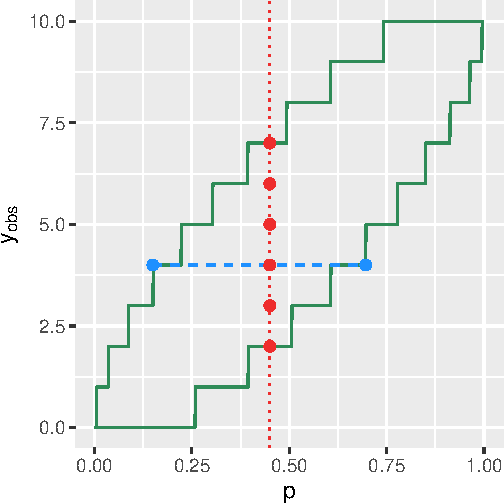
\includegraphics[keepaspectratio]{03-binomial_files/figure-latex/fig-disccicover-1.pdf}}

}

\caption{\label{fig-disccicover}An illustration of the relationship
between hypothesis testing and confidence interval estimation for a
discrete sampling distribution (here, a binomial distribution with
\(k=10\)). The two green lines define rejection-region boundaries for a
two-sided test with null hypothesis parameter value \(p\). Assume
\(p = 0.45\): the red dots indicates the values of \(y_{\mathrm{obs}}\)
in the acceptance region (where we fail to reject the null). The
horizontal dashed blue line shows the confidence interval constructed
for a given value of \(y_{\mathrm{obs}}\). Given \(p\), the probability
of sampling a statistic in the acceptance region is generally greater
than \(1-\alpha\), and thus the coverage of confidence intervals, which
has the same value, will also be generally greater than \(1-\alpha\).}

\end{figure}%

The blue dashed line in Figure~\ref{fig-disccicover} is an example of a
confidence interval (specifically for \(y_{\mathrm{obs}} = 4\)). In
order to construct an interval like this, we would use a
\texttt{uniroot()}-style code as we have before, but we would
potentially change the value of the observed statistic, as displayed
below.

{\def\LTcaptype{none} % do not increment counter
\begin{longtable}[]{@{}ccc@{}}
\toprule\noalign{}
\endhead
\bottomrule\noalign{}
\endlastfoot
& lower bound & upper bound \\
yes line & \(y_{\mathrm{obs}}-a\) & \(y_{\mathrm{obs}}\) \\
no line & \(y_{\mathrm{obs}}\) & \(y_{\mathrm{obs}}-a\) \\
\end{longtable}
}

The value \(a\) is the difference between the observed statistic value
and the next lower value in the sampling distribution's domain; for a
binomial distribution, \(a = 1\). (Refer to
Section~\ref{sec-chap1confref} for the meanings of ``yes line'' and ``no
line.'')

We note that for the specific case of the binomial distribution, the
confidence intervals that we construct are dubbed \emph{exact}, or
\emph{Clopper-Pearson}, intervals. Because binomial distributions have
historically been difficult to work with analytically, a number of
algorithms have been developed through the years for constructing
approximate confidence intervals for binomial probabilities. (See, e.g.,
\href{https://en.wikipedia.org/wiki/Binomial_proportion_confidence_interval}{this
Wikipedia page} for examples.) It is our opinion that there is no reason
to utilize \emph{any} of these algorithms when one can compute exact
intervals, particularly since the coverages of exact intervals are
easily derived for any given value \(p\). However, for completeness, we
illustrate how one would construct the most-commonly used approximating
interval, the \emph{Wald interval}, in an example below.

For more on confidence intervals, go to
Section~\ref{sec-chap4confidence}.

\subsection{Examples}\label{examples-32}

\subsubsection{Binomial Probability: Confidence
Interval}\label{binomial-probability-confidence-interval}

\begin{quote}
Assume that we sample \(n\) iid data from a binomial distribution with
number of trials \(k\) and probability \(p\). Then, as shown above,
\(Y = \sum_{i=1}^n X_i \sim\) Binom(\(nk,p\)); our observed test
statistic is \(y_{\mathrm{obs}} = \sum_{i=1}^n x_i\). For this
statistic, \(E[Y] = nkp\) increases with \(p\), so \(q = 1-\alpha/2\)
maps to the lower bound, while \(q = \alpha/2\) maps to the upper bound.
\end{quote}

\begin{Shaded}
\begin{Highlighting}[]
\CommentTok{\# generate data; typically, X would be provided}
\FunctionTok{set.seed}\NormalTok{(}\DecValTok{101}\NormalTok{)}
\NormalTok{n     }\OtherTok{\textless{}{-}} \DecValTok{12}
\NormalTok{k     }\OtherTok{\textless{}{-}} \DecValTok{5}
\NormalTok{p     }\OtherTok{\textless{}{-}} \FloatTok{0.4}
\NormalTok{X     }\OtherTok{\textless{}{-}} \FunctionTok{rbinom}\NormalTok{(n, }\AttributeTok{size =}\NormalTok{ k, }\AttributeTok{prob =}\NormalTok{ p)}

\CommentTok{\# construct 95\% interval}
\NormalTok{alpha }\OtherTok{\textless{}{-}} \FloatTok{0.05}
\NormalTok{Y     }\OtherTok{\textless{}{-}} \FunctionTok{sum}\NormalTok{(X)}

\NormalTok{f }\OtherTok{\textless{}{-}} \ControlFlowTok{function}\NormalTok{(p, k, n, y.obs, q)}
\NormalTok{\{}
  \FunctionTok{pbinom}\NormalTok{(y.obs, }\AttributeTok{size =}\NormalTok{ n }\SpecialCharTok{*}\NormalTok{ k, }\AttributeTok{prob =}\NormalTok{ p) }\SpecialCharTok{{-}}\NormalTok{ q}
\NormalTok{\}}

\CommentTok{\# note discreteness correction in first function call below}
\FunctionTok{round}\NormalTok{(}\FunctionTok{uniroot}\NormalTok{(f, }\AttributeTok{interval =} \FunctionTok{c}\NormalTok{(}\DecValTok{0}\NormalTok{, }\DecValTok{1}\NormalTok{), }\AttributeTok{k =}\NormalTok{ k, }\AttributeTok{n =}\NormalTok{ n,}
              \AttributeTok{y.obs =}\NormalTok{ Y }\SpecialCharTok{{-}} \DecValTok{1}\NormalTok{, }\AttributeTok{q =} \DecValTok{1} \SpecialCharTok{{-}}\NormalTok{ alpha }\SpecialCharTok{/} \DecValTok{2}\NormalTok{)}\SpecialCharTok{$}\NormalTok{root, }\DecValTok{3}\NormalTok{)}
\end{Highlighting}
\end{Shaded}

\begin{verbatim}
[1] 0.246
\end{verbatim}

\begin{Shaded}
\begin{Highlighting}[]
\FunctionTok{round}\NormalTok{(}\FunctionTok{uniroot}\NormalTok{(f, }\AttributeTok{interval =} \FunctionTok{c}\NormalTok{(}\DecValTok{0}\NormalTok{, }\DecValTok{1}\NormalTok{), }\AttributeTok{k =}\NormalTok{ k, }\AttributeTok{n =}\NormalTok{ n,}
              \AttributeTok{y.obs =}\NormalTok{ Y,     }\AttributeTok{q =}\NormalTok{     alpha }\SpecialCharTok{/} \DecValTok{2}\NormalTok{)}\SpecialCharTok{$}\NormalTok{root, }\DecValTok{3}\NormalTok{)}
\end{Highlighting}
\end{Shaded}

\begin{verbatim}
[1] 0.501
\end{verbatim}

\begin{quote}
We find that the interval is \([\hat{p}_L,\hat{p}_U] =
[0.246,0.501]\), which overlaps the true value of 0.4. (See
Figure~\ref{fig-binci}.) Note that, unlike in
Section~\ref{sec-chap2confidence}, the interval over which we search for
the root is {[}0,1{]}, which is the range of possible values for \(p\).
\end{quote}

\begin{quote}
We can compute the coverage of this interval following the prescription
given above, assuming \(p = 0.4\):
\end{quote}

\begin{Shaded}
\begin{Highlighting}[]
\NormalTok{y.rr.lo }\OtherTok{\textless{}{-}} \FunctionTok{qbinom}\NormalTok{(    alpha }\SpecialCharTok{/} \DecValTok{2}\NormalTok{, n }\SpecialCharTok{*}\NormalTok{ k, p)}
\NormalTok{y.rr.hi }\OtherTok{\textless{}{-}} \FunctionTok{qbinom}\NormalTok{(}\DecValTok{1} \SpecialCharTok{{-}}\NormalTok{ alpha }\SpecialCharTok{/} \DecValTok{2}\NormalTok{, n }\SpecialCharTok{*}\NormalTok{ k, p)}
\FunctionTok{round}\NormalTok{(}\FunctionTok{sum}\NormalTok{(}\FunctionTok{dbinom}\NormalTok{(y.rr.lo}\SpecialCharTok{:}\NormalTok{y.rr.hi, n }\SpecialCharTok{*}\NormalTok{ k, p)), }\DecValTok{3}\NormalTok{)}
\end{Highlighting}
\end{Shaded}

\begin{verbatim}
[1] 0.965
\end{verbatim}

\begin{quote}
Due to the discreteness of the binomial distribution, the true coverage
of our intervals (given \(n = 12\), \(k = 5\), and \(p = 0.4\)) is
96.5\%, not 95\%.
\end{quote}

\begin{figure}

\begin{minipage}[t]{0.50\linewidth}

\centering{

\pandocbounded{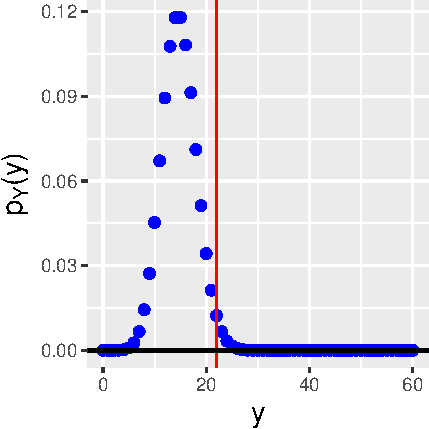
\includegraphics[keepaspectratio]{03-binomial_files/figure-latex/fig-binci-1.pdf}}

}

\subcaption{\label{fig-binci-1}}

\end{minipage}%
%
\begin{minipage}[t]{0.50\linewidth}

\centering{

\pandocbounded{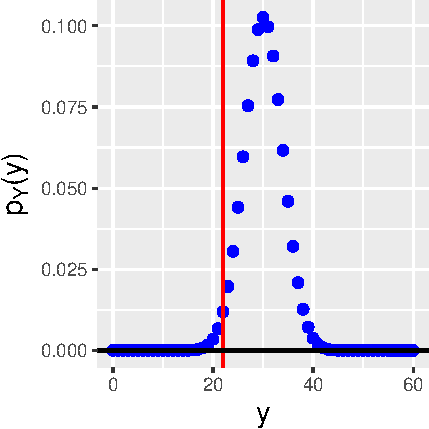
\includegraphics[keepaspectratio]{03-binomial_files/figure-latex/fig-binci-2.pdf}}

}

\subcaption{\label{fig-binci-2}}

\end{minipage}%

\caption{\label{fig-binci}Probability mass functions for binomial
distributions for which \(n \cdot k= 12 \cdot 5 = 60\) and (a)
\(p=0.246\) and (b) \(p=0.501\). We observe
\(y_{\mathrm{obs}} = \sum_{i=1}^n x_i = 22\) successes and we want to
construct a 95\% confidence interval. \(p=0.246\) is the smallest value
of \(p\) such that \(F_Y^{-1}(0.975) = 22\), while \(p=0.501\) is the
largest value of \(p\) such that \(F_Y^{-1}(0.025) = 22\).}

\end{figure}%

\subsubsection{Binomial Probability: Wald
Interval}\label{binomial-probability-wald-interval}

\begin{quote}
Let's assume that we have sampled \(n\) iid binomial variables with
number of trials \(k\) and success probability \(p\). When \(k\) is
sufficiently large and \(p\) is sufficiently far from 0 or 1, we can
assume that \(\bar{X}\) has a distribution whose shape is approximately
that of a normal distribution, with mean \(E[\bar{X}] = kp\) and with
variance and standard error \[
V[\bar{X}] = \frac{kp(1-p)}{n} ~~~ \mbox{and} ~~~ se(\bar{X}) = \sqrt{V[\bar{X}]} = \sqrt{\frac{kp(1-p)}{n}} \,. 
\] Furthermore, we can assume that \(\hat{p} = \bar{X}/k\) is
approximately normally distributed, with mean \(p\), variance
\(V[\hat{p}] = V[\bar{X}]/k^2 = p(1-p)/nk\), and standard error
\(\sqrt{p(1-p)/nk}\). Given this information, it is simple to express,
e.g., an approximate two-sided \(100(1-\alpha)\)\% confidence interval
for \(p\): \[
\hat{p} \pm z_{1-\alpha/2} se(\hat{p}) ~~ \Rightarrow ~~ \left[ \hat{p} - z_{1-\alpha/2} \sqrt{\frac{p(1-p)}{nk}} \, , \, \hat{p} + z_{1-\alpha/2} \sqrt{\frac{p(1-p)}{nk}} \right] \,,
\] where \(z_{1-\alpha/2} = \Phi^{-1}(1-\alpha/2)\). However, we don't
actually know the true value of \(p\)\ldots so we plug in
\(p = \hat{p}\).
\end{quote}

\begin{quote}
This is the so-called \emph{Wald interval} that is typically provided to
students in introductory statistics courses, although it is typically
provided assuming \(n = 1\) and assuming that \(\alpha = 0.05\): \[
\left[ \hat{p} - 1.96 \sqrt{\frac{\hat{p}(1-\hat{p})}{k}} \, , \, \hat{p} + 1.96 \sqrt{\frac{\hat{p}(1-\hat{p})}{k}} \right] \,,
\] where in this case \(\hat{p} = X/k\).
\end{quote}

\begin{quote}
What is the Wald interval for the situation provided in the first
example above?
\end{quote}

\begin{Shaded}
\begin{Highlighting}[]
\CommentTok{\# generate data}
\FunctionTok{set.seed}\NormalTok{(}\DecValTok{101}\NormalTok{)}
\NormalTok{n     }\OtherTok{\textless{}{-}} \DecValTok{12}
\NormalTok{k     }\OtherTok{\textless{}{-}} \DecValTok{5}
\NormalTok{p     }\OtherTok{\textless{}{-}} \FloatTok{0.4}
\NormalTok{X     }\OtherTok{\textless{}{-}} \FunctionTok{rbinom}\NormalTok{(n, }\AttributeTok{size =}\NormalTok{ k, }\AttributeTok{prob =}\NormalTok{ p)}

\CommentTok{\# compute 95\% interval}
\NormalTok{alpha }\OtherTok{\textless{}{-}} \FloatTok{0.05}
\NormalTok{z     }\OtherTok{\textless{}{-}} \FunctionTok{qnorm}\NormalTok{(}\DecValTok{1} \SpecialCharTok{{-}}\NormalTok{ alpha }\SpecialCharTok{/} \DecValTok{2}\NormalTok{)}
\NormalTok{p.hat }\OtherTok{\textless{}{-}} \FunctionTok{sum}\NormalTok{(X) }\SpecialCharTok{/}\NormalTok{ (n }\SpecialCharTok{*}\NormalTok{ k)}

\FunctionTok{round}\NormalTok{(p.hat }\SpecialCharTok{+} \FunctionTok{c}\NormalTok{(}\SpecialCharTok{{-}}\DecValTok{1}\NormalTok{, }\DecValTok{1}\NormalTok{) }\SpecialCharTok{*}\NormalTok{ z }\SpecialCharTok{*} \FunctionTok{sqrt}\NormalTok{(p.hat }\SpecialCharTok{*}\NormalTok{ (}\DecValTok{1} \SpecialCharTok{{-}}\NormalTok{ p.hat) }\SpecialCharTok{/}\NormalTok{ (n }\SpecialCharTok{*}\NormalTok{ k)), }\DecValTok{3}\NormalTok{)}
\end{Highlighting}
\end{Shaded}

\begin{verbatim}
[1] 0.245 0.489
\end{verbatim}

\begin{quote}
We compare these values to those generated in the first example:
\([0.236,0.501]\). Here, the interval is smaller relative to the
Clopper-Pearson interval, and thus the coverage for \(p = 0.4\) (which
we would have to estimate via simulation) will be smaller as well.
\end{quote}

\subsubsection{Negative Binomial Probability: Confidence
Interval}\label{negative-binomial-probability-confidence-interval}

\begin{quote}
Let's assume that we have performed \(n = 12\) separate negative
binomial trials, each with a target number of successes \(s = 5\), and
recorded the number of failures \(X_1,\ldots,X_{n}\) for each. Below we
will show how to compute the confidence interval for the success
probability \(p\), but before we start, we recall that
\(Y = X_+ = \sum_{i=1}^n X_i\) is a negative binomially distributed
random variable for \(ns\) successes and success probability \(p\).
Here, \(E[Y] = s(1-p)/p\)\ldots as \(p\) increases, \(E[Y]\)
\emph{decreases}. Thus when we adapt the confidence interval code we use
for binomially distributed data, we need to switch the mapping of
\(q = 1-\alpha/2\) and \(q = \alpha/2\) to the \emph{upper} and
\emph{lower} bounds, respectively.
\end{quote}

\begin{Shaded}
\begin{Highlighting}[]
\CommentTok{\# generate data}
\FunctionTok{set.seed}\NormalTok{(}\DecValTok{101}\NormalTok{)}
\NormalTok{n     }\OtherTok{\textless{}{-}} \DecValTok{12}
\NormalTok{s     }\OtherTok{\textless{}{-}} \DecValTok{5}
\NormalTok{p     }\OtherTok{\textless{}{-}} \FloatTok{0.4}
\NormalTok{X     }\OtherTok{\textless{}{-}} \FunctionTok{rnbinom}\NormalTok{(n, }\AttributeTok{size =}\NormalTok{ s, }\AttributeTok{prob =}\NormalTok{ p)}

\CommentTok{\# compute 95\% interval}
\NormalTok{alpha }\OtherTok{\textless{}{-}} \FloatTok{0.05}
\NormalTok{Y     }\OtherTok{\textless{}{-}} \FunctionTok{sum}\NormalTok{(X)}

\NormalTok{f }\OtherTok{\textless{}{-}} \ControlFlowTok{function}\NormalTok{(p, s, n, y.obs, q)}
\NormalTok{\{     }
  \FunctionTok{pnbinom}\NormalTok{(y.obs, }\AttributeTok{size =}\NormalTok{ n }\SpecialCharTok{*}\NormalTok{ s, }\AttributeTok{prob =}\NormalTok{ p) }\SpecialCharTok{{-}}\NormalTok{ q}
\NormalTok{\}     }

\CommentTok{\# note discreteness correction in second function call below}
\FunctionTok{round}\NormalTok{(}\FunctionTok{uniroot}\NormalTok{(f, }\AttributeTok{interval =} \FunctionTok{c}\NormalTok{(}\FloatTok{0.0001}\NormalTok{, }\DecValTok{1}\NormalTok{), }\AttributeTok{s =}\NormalTok{ s, }\AttributeTok{n =}\NormalTok{ n,}
              \AttributeTok{y.obs =}\NormalTok{ Y    , }\AttributeTok{q =}\NormalTok{     alpha }\SpecialCharTok{/} \DecValTok{2}\NormalTok{)}\SpecialCharTok{$}\NormalTok{root, }\DecValTok{3}\NormalTok{)}
\end{Highlighting}
\end{Shaded}

\begin{verbatim}
[1] 0.326
\end{verbatim}

\begin{Shaded}
\begin{Highlighting}[]
\FunctionTok{round}\NormalTok{(}\FunctionTok{uniroot}\NormalTok{(f, }\AttributeTok{interval =} \FunctionTok{c}\NormalTok{(}\FloatTok{0.0001}\NormalTok{, }\DecValTok{1}\NormalTok{), }\AttributeTok{s =}\NormalTok{ s, }\AttributeTok{n =}\NormalTok{ n,}
              \AttributeTok{y.obs =}\NormalTok{ Y }\SpecialCharTok{{-}} \DecValTok{1}\NormalTok{, }\AttributeTok{q =} \DecValTok{1} \SpecialCharTok{{-}}\NormalTok{ alpha }\SpecialCharTok{/} \DecValTok{2}\NormalTok{)}\SpecialCharTok{$}\NormalTok{root, }\DecValTok{3}\NormalTok{) }
\end{Highlighting}
\end{Shaded}

\begin{verbatim}
[1] 0.485
\end{verbatim}

\begin{quote}
The confidence interval is \([\hat{p}_L,\hat{p}_U] = [0.326,0.485]\),
which overlaps the true value 0.4. We note that in the code, we change
the lower bound on the interval from 0 (in the binomial case) to 0.0001
(something suitably small but non-zero): a probability of success of 0
maps to an infinite number of failures, which \texttt{R} cannot
tolerate!
\end{quote}

\begin{quote}
We can compute the coverage of this interval following the prescription
given above:
\end{quote}

\begin{Shaded}
\begin{Highlighting}[]
\NormalTok{y.rr.lo }\OtherTok{\textless{}{-}} \FunctionTok{qnbinom}\NormalTok{(}\DecValTok{1} \SpecialCharTok{{-}}\NormalTok{ alpha }\SpecialCharTok{/} \DecValTok{2}\NormalTok{, n }\SpecialCharTok{*}\NormalTok{ s, p)}
\NormalTok{y.rr.hi }\OtherTok{\textless{}{-}} \FunctionTok{qnbinom}\NormalTok{(    alpha }\SpecialCharTok{/} \DecValTok{2}\NormalTok{, n }\SpecialCharTok{*}\NormalTok{ s, p)}
\FunctionTok{round}\NormalTok{(}\FunctionTok{sum}\NormalTok{(}\FunctionTok{dnbinom}\NormalTok{(y.rr.lo}\SpecialCharTok{:}\NormalTok{y.rr.hi, n }\SpecialCharTok{*}\NormalTok{ s, p)), }\DecValTok{3}\NormalTok{)}
\end{Highlighting}
\end{Shaded}

\begin{verbatim}
[1] 0.951
\end{verbatim}

\begin{quote}
Due to the discreteness of the negative binomial distribution, the true
coverage in this instance is 95.1\%, not 95\%.
\end{quote}

\begin{figure}

\begin{minipage}[t]{0.50\linewidth}

\centering{

\pandocbounded{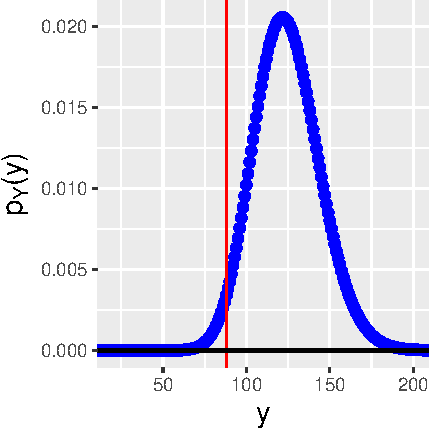
\includegraphics[keepaspectratio]{03-binomial_files/figure-latex/fig-nbinci-1.pdf}}

}

\subcaption{\label{fig-nbinci-1}}

\end{minipage}%
%
\begin{minipage}[t]{0.50\linewidth}

\centering{

\pandocbounded{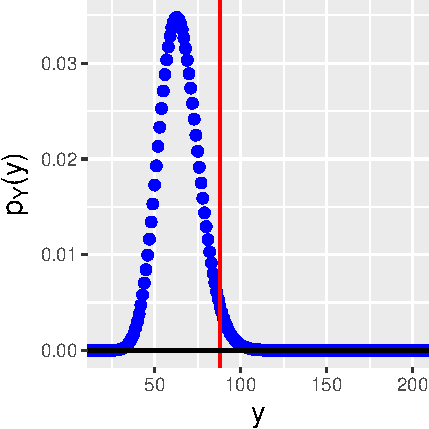
\includegraphics[keepaspectratio]{03-binomial_files/figure-latex/fig-nbinci-2.pdf}}

}

\subcaption{\label{fig-nbinci-2}}

\end{minipage}%

\caption{\label{fig-nbinci}Probability mass functions for negative
binomial distributions for which \(n \cdot s = 12 \cdot 5 = 60\) and (a)
\(p=0.326\) and (b) \(p=0.485\). We observe
\(y_{\mathrm{obs}} = \sum_{i=1}^n x_i = 88\) failures and we want to
construct a 95\% confidence interval. \(p=0.326\) is the smallest value
of \(p\) such that \(F_Y^{-1}(0.025) = 88\), while \(p=0.485\) is the
largest value of \(p\) such that \(F_Y^{-1}(0.975) = 88\).}

\end{figure}%

\subsubsection{Hypergeometric Distribution: Number of
Successes}\label{hypergeometric-distribution-number-of-successes}

\begin{quote}
Let's suppose that we have a collection of \(K = 200\) objects, and that
when we sample \(k = 10\) of them without replacement, we find that
\(x = 3\) of them are defective. (We are assuming that finding a
defective object is a ``success.'') The question: what is the overall
number of defective objects in the collection?
\end{quote}

\begin{quote}
To begin to answer this question, we will construct a 95\% two-sided
confidence interval for the total number of successes \(s\). Our test
statistic is \(Y = X\), which has the observed value
\(y_{\mathrm{obs}} = 3\). Recall that the expected value for \(X\) is
\(E[X] = ks/K\); as \(s\) increases, the expected value increases, so we
are on the ``yes'' line of the reference table. At this point, we have
all the information we need to construct our interval:
\end{quote}

\begin{Shaded}
\begin{Highlighting}[]
\NormalTok{alpha }\OtherTok{\textless{}{-}} \FloatTok{0.05}
\NormalTok{K     }\OtherTok{\textless{}{-}} \DecValTok{200}
\NormalTok{k     }\OtherTok{\textless{}{-}} \DecValTok{10}
\NormalTok{X     }\OtherTok{\textless{}{-}} \DecValTok{3}

\NormalTok{f }\OtherTok{\textless{}{-}} \ControlFlowTok{function}\NormalTok{(s, K, k, y.obs, q) }
\NormalTok{\{}
  \FunctionTok{phyper}\NormalTok{(y.obs, s, K }\SpecialCharTok{{-}}\NormalTok{ s, k) }\SpecialCharTok{{-}}\NormalTok{ q}
\NormalTok{\}}

\FunctionTok{round}\NormalTok{(}\FunctionTok{uniroot}\NormalTok{(f, }\AttributeTok{interval =} \FunctionTok{c}\NormalTok{(X, K }\SpecialCharTok{{-}}\NormalTok{ (k }\SpecialCharTok{{-}}\NormalTok{ X)), }\AttributeTok{K =}\NormalTok{ K, }\AttributeTok{k =}\NormalTok{ k,}
              \AttributeTok{y.obs =}\NormalTok{ X }\SpecialCharTok{{-}} \DecValTok{1}\NormalTok{, }\AttributeTok{q =} \DecValTok{1} \SpecialCharTok{{-}}\NormalTok{ alpha }\SpecialCharTok{/} \DecValTok{2}\NormalTok{)}\SpecialCharTok{$}\NormalTok{root, }\DecValTok{3}\NormalTok{)}
\end{Highlighting}
\end{Shaded}

\begin{verbatim}
[1] 14.5
\end{verbatim}

\begin{Shaded}
\begin{Highlighting}[]
\FunctionTok{round}\NormalTok{(}\FunctionTok{uniroot}\NormalTok{(f, }\AttributeTok{interval =} \FunctionTok{c}\NormalTok{(X, K }\SpecialCharTok{{-}}\NormalTok{ (k }\SpecialCharTok{{-}}\NormalTok{ X)), }\AttributeTok{K =}\NormalTok{ K, }\AttributeTok{k =}\NormalTok{ k,}
              \AttributeTok{y.obs =}\NormalTok{ X,     }\AttributeTok{q =}\NormalTok{     alpha }\SpecialCharTok{/} \DecValTok{2}\NormalTok{)}\SpecialCharTok{$}\NormalTok{root, }\DecValTok{3}\NormalTok{)}
\end{Highlighting}
\end{Shaded}

\begin{verbatim}
[1] 129.5
\end{verbatim}

\begin{quote}
Our 95\% confidence interval is \([14.5,129.5]\): with so few observed
data, we cannot tightly constrain the overall number of defective
objects in the collection.
\end{quote}

\subsubsection{Order Statistic: Confidence
Interval}\label{order-statistic-confidence-interval}

\begin{quote}
In an example above, we determined the probability density function of
the \(j = 70^{\mathrm{th}}\) ordered datum, given \(n = 200\) data
sampled according to a standard normal distribution. Here, we will
change this up a bit: if, for instance, we assume that we are sampling
data according to a \(\mathcal{N}(\mu,1)\) distribution, and the value
of the \(70^{\mathrm{th}}\) ordered datum is
\(x_{(70),\mathrm{obs}} = -0.5\), what would be a 95\% two-sided
confidence interval for \(\mu\)?
\end{quote}

\begin{quote}
As the reader will see in the code below, the only difference between
this calculation and previous ones is that instead of adopting a
pre-existing \texttt{R} code for the cdf in the expression
\(F_Y(y_{\mathrm{obs}} \vert \theta) - q\), we define our own cdf code,
which we base on the expression for the cdf of an order statistic given
previously in this chapter, in Section~\ref{sec-chap3order}.
\end{quote}

\begin{Shaded}
\begin{Highlighting}[]
\NormalTok{alpha }\OtherTok{\textless{}{-}} \FloatTok{0.05}

\CommentTok{\# function returning the cdf for an order statistic}
\NormalTok{F }\OtherTok{\textless{}{-}} \ControlFlowTok{function}\NormalTok{(x, j, n, mu)}
\NormalTok{\{}
\NormalTok{  F.j }\OtherTok{\textless{}{-}} \DecValTok{0}
  \ControlFlowTok{for}\NormalTok{ ( ii }\ControlFlowTok{in}\NormalTok{ j}\SpecialCharTok{:}\NormalTok{n ) \{}
\NormalTok{    F.j }\OtherTok{\textless{}{-}}\NormalTok{ F.j }\SpecialCharTok{+} \FunctionTok{choose}\NormalTok{(n, ii) }\SpecialCharTok{*}\NormalTok{ (}\FunctionTok{pnorm}\NormalTok{(x, mu, }\DecValTok{1}\NormalTok{))}\SpecialCharTok{\^{}}\NormalTok{ii }\SpecialCharTok{*}\NormalTok{ (}\DecValTok{1} \SpecialCharTok{{-}} \FunctionTok{pnorm}\NormalTok{(x, mu, }\DecValTok{1}\NormalTok{))}\SpecialCharTok{\^{}}\NormalTok{(n}\SpecialCharTok{{-}}\NormalTok{ii)}
\NormalTok{  \}}
  \FunctionTok{return}\NormalTok{(F.j)}
\NormalTok{\}}

\NormalTok{f }\OtherTok{\textless{}{-}} \ControlFlowTok{function}\NormalTok{(mu, j, n, y.obs, q)}
\NormalTok{\{}
  \FunctionTok{F}\NormalTok{(y.obs, j, n, mu) }\SpecialCharTok{{-}}\NormalTok{ q}
\NormalTok{\}}

\FunctionTok{round}\NormalTok{(}\FunctionTok{uniroot}\NormalTok{(f, }\AttributeTok{interval =} \FunctionTok{c}\NormalTok{(}\SpecialCharTok{{-}}\DecValTok{10}\NormalTok{, }\DecValTok{10}\NormalTok{), }\AttributeTok{j =} \DecValTok{70}\NormalTok{, }\AttributeTok{n =} \DecValTok{200}\NormalTok{,}
              \AttributeTok{y.obs =} \SpecialCharTok{{-}}\FloatTok{0.5}\NormalTok{, }\AttributeTok{q =} \DecValTok{1} \SpecialCharTok{{-}}\NormalTok{ alpha }\SpecialCharTok{/} \DecValTok{2}\NormalTok{)}\SpecialCharTok{$}\NormalTok{root, }\DecValTok{3}\NormalTok{)}
\end{Highlighting}
\end{Shaded}

\begin{verbatim}
[1] -0.286
\end{verbatim}

\begin{Shaded}
\begin{Highlighting}[]
\FunctionTok{round}\NormalTok{(}\FunctionTok{uniroot}\NormalTok{(f, }\AttributeTok{interval =} \FunctionTok{c}\NormalTok{(}\SpecialCharTok{{-}}\DecValTok{10}\NormalTok{, }\DecValTok{10}\NormalTok{), }\AttributeTok{j =} \DecValTok{70}\NormalTok{, }\AttributeTok{n =} \DecValTok{200}\NormalTok{,}
              \AttributeTok{y.obs =} \SpecialCharTok{{-}}\FloatTok{0.5}\NormalTok{, }\AttributeTok{q =}\NormalTok{     alpha }\SpecialCharTok{/} \DecValTok{2}\NormalTok{)}\SpecialCharTok{$}\NormalTok{root, }\DecValTok{3}\NormalTok{)}
\end{Highlighting}
\end{Shaded}

\begin{verbatim}
[1] 0.071
\end{verbatim}

\begin{quote}
Our 95\% two-sided confidence interval for \(\mu\) is
\([-0.286,0.071]\). We note (and the interested reader can confirm) that
as we go from \(j = 1\) (the minimum value) to \(j = 200\) (the maximum
value), the interval widths will systematically get smaller, on average,
and then, after \(j \approx 100\), will systematically get larger. This
makes intuitive sense: the minimum and maximum values will of course be
less informative about the population mean than the values around the
sample median. However, despite this, because the exact sampling
distribution is known for all values of \(j\), the coverage of each of
the intervals will be exactly 95\%.
\end{quote}

\subsubsection{Order Statistics: Distribution-Free Confidence Interval
for
Percentiles}\label{order-statistics-distribution-free-confidence-interval-for-percentiles}

\begin{quote}
Let's revisit the data that we generated in an example in the last
section:
\end{quote}

\begin{verbatim}
 [1] 0.275 0.430 0.687 0.717 1.252 1.275 1.386 2.262 3.327 3.447 4.127
\end{verbatim}

\begin{quote}
In that example, we determined that 2.7945 is a (biased) point estimate
for the underlying distribution's \(75^{\mathrm{th}}\) percentile,
\(\chi_{0.75}\). Here, we will show how one can utilize order statistics
and the binomial distribution to construct a confidence interval for
this quantity.
\end{quote}

\begin{quote}
Let \(q\) represent a quantile and let \(\chi_q\) be its associated
100\(q^{\mathrm{th}}\) distribution percentile. Our goal is to define an
interval \(X_{(i)} \leq \chi_q \leq X_{(j)}\) such that \begin{align*}
i &= {\mathrm{sup}}\{ k \in [1,n] \vert P(X_{(i)} > \chi_q) < \frac{\alpha}{2} \} \\
j &= {\mathrm{inf}}\{ k \in [1,n] \vert P(X_{(j)} < \chi_q) < \frac{\alpha}{2} \} \,.
\end{align*} Let's examine the first line. Here, \(P(X_{(i)} > \chi_q)\)
represents the probability that at least \(i\) out of \(n\) observations
have values greater than \(\chi_q\). The smallest value of the defined
set is given by the generalized inverse cumulative distribution
function, with input \(\alpha/2\); in \texttt{R} code:
\end{quote}

\begin{Shaded}
\begin{Highlighting}[]
\NormalTok{alpha }\OtherTok{\textless{}{-}} \FloatTok{0.05}
\NormalTok{q     }\OtherTok{\textless{}{-}} \FloatTok{0.75}
\FunctionTok{qbinom}\NormalTok{(alpha }\SpecialCharTok{/} \DecValTok{2}\NormalTok{, n, q)}
\end{Highlighting}
\end{Shaded}

\begin{verbatim}
[1] 5
\end{verbatim}

\begin{quote}
Similar reasoning yields a value for \(j\):
\end{quote}

\begin{Shaded}
\begin{Highlighting}[]
\FunctionTok{qbinom}\NormalTok{(}\DecValTok{1} \SpecialCharTok{{-}}\NormalTok{ alpha }\SpecialCharTok{/} \DecValTok{2}\NormalTok{, n, q)}
\end{Highlighting}
\end{Shaded}

\begin{verbatim}
[1] 11
\end{verbatim}

\begin{quote}
Hence a distribution-free 95\% two-sided interval estimate for
\(\chi_{0.75}\) is
\end{quote}

\begin{Shaded}
\begin{Highlighting}[]
\FunctionTok{cat}\NormalTok{(}\StringTok{"["}\NormalTok{, X[}\FunctionTok{qbinom}\NormalTok{(alpha }\SpecialCharTok{/} \DecValTok{2}\NormalTok{, n, q)], }\StringTok{","}\NormalTok{, X[}\FunctionTok{qbinom}\NormalTok{(}\DecValTok{1} \SpecialCharTok{{-}}\NormalTok{ alpha }\SpecialCharTok{/} \DecValTok{2}\NormalTok{, n, q)], }\StringTok{"]}\SpecialCharTok{\textbackslash{}n}\StringTok{"}\NormalTok{)}
\end{Highlighting}
\end{Shaded}

\begin{verbatim}
[ 1.252 , 4.127 ]
\end{verbatim}

\begin{quote}
Since the sampling distribution for the number of data that have values
less than \(\chi_q\) is known exactly (it's a binomial distribution),
the coverage of intervals constructed like the one above will be
\(\geq 1-\alpha\) (but not \(= 1-\alpha\) since we are working with a
discrete sampling distribution).
\end{quote}

\begin{quote}
We note in passing that it can be the case that one can sometimes
construct shorter confidence intervals that still have coverage
\(\geq 1-\alpha\) by removing the requirement that the tail summations
be \(< \alpha/2\) on either side of the interval. Such intervals would
still be valid because there is no theoretical requirement that
\(\alpha\) be ``split evenly'' to define lower and upper interval
bounds\ldots it is just standard practice to make an even split.
\end{quote}

\section{Hypothesis Testing: Neyman-Pearson
Lemma}\label{sec-chap3nplemma}

What to take away from this section:

\begin{itemize}
\item
  The \emph{Neyman-Pearson lemma} states that a ratio of likelihood
  functions constitutes \textbf{the most powerful test} of the simple
  hypotheses \(H_o : \theta = \theta_o\) and
  \(H_a : \theta = \theta_a\).
\item
  If the rejection region associated with this most powerful test is not
  a function of \(\theta_a\), then the test we define is a
  \emph{uniformly most powerful test}.
\item
  If we are working with a member of the exponential family of
  distributions, then the NP lemma is telling us that we should simply
  conduct a hypothesis test in the manner described in
  Section~\ref{sec-chap1hypothesis} and
  Section~\ref{sec-chap2hypothesis} while utilizing a \emph{sufficient
  statistic} for \(\theta\).
\end{itemize}

For previous material on hypothesis testing, see
Section~\ref{sec-chap2hypothesis}.

\smallskip\hrule

\begin{quote}
\textbf{Recall}: \emph{a hypothesis test is a framework to make an
inference about the value of a population parameter \(\theta\). The null
hypothesis \(H_o\) is that \(\theta = \theta_o\), while possible
alternatives \(H_a\) are \(\theta \neq \theta_o\) (two-tail test),
\(\theta > \theta_o\) (upper-tail test), and \(\theta < \theta_o\)
(lower-tail test). For, e.g., a one-tail test, we reject the null
hypothesis if the observed test statistic \(y_{\mathrm{obs}}\) falls
outside the bound given by \(y_{RR}\), which is a solution to the
equation} \[
F_Y(y_{RR} \vert \theta_o) - q = 0 \,,
\] \emph{where \(F_Y(\cdot)\) is the cumulative distribution function
for the statistic \(Y\) and \(q\) is an appropriate quantile value that
is a function of the adopted Type I error rate \(\alpha\). Note that the
hypothesis test framework only allows us to make a decision about a null
hypothesis; nothing is proven.}
\end{quote}

\smallskip\hrule

In Section~\ref{sec-chap2hypothesis}, we utilized \(\bar{X}\) when
testing hypotheses about the normal mean \(\mu\). This is a principled
choice for a test statistic\(-\)after all, \(\bar{X}\) is the MLE for
\(\mu-\)but can we choose a better one?

To help answer this question, we now introduce a method for defining the
\emph{most powerful test} of a \emph{simple} null hypothesis versus a
\emph{simple} alternative hypothesis: \[
H_o : \theta = \theta_o ~~\mbox{and}~~ H_a : \theta = \theta_a \,.
\] Note that the word ``simple'' has a precise meaning here: it means
that when we set \(\theta\) to a particular value, we are
\emph{completely fixing the shape and location of the pmf or pdf from
which the data are sampled}. If, for instance, we are dealing with a
normal distribution with unknown variance \(\sigma^2\), the hypothesis
\(\mu = \mu_o\) would not be simple, since the width of the pdf can
still vary: the shape is not completely fixed. (The hypothesis
\(\mu = \mu_o\) with variance unknown is dubbed a \emph{composite}
hypothesis. We will discuss the more general case wherein we work with
composite hypotheses in Section~\ref{sec-chap4hypothesis}.) For a given
test level \(\alpha\), the \emph{Neyman-Pearson lemma} states that the
test with the most power has a rejection region of the form \[
\lambda_{NP} = \frac{\mathcal{L}(\theta_o \vert \mathbf{x})}{\mathcal{L}(\theta_a \vert \mathbf{x})} < c(\alpha) \,,
\] where \(c\) is a constant that we must determine, one whose value is
a function of \(\alpha\). While this formulation initially appears
straightforward, it is in fact not necessarily clear how to derive
\(c(\alpha)\). However: when we work with distributions that belong to
the exponential family, \emph{we don't have to}! The NP lemma utilizes
the likelihood function, so in this situation it is implicitly telling
us that \emph{the best statistic for differentiating between two simple
hypotheses is a sufficient statistic}. We simply determine a sufficient
statistic and use its sampling distribution to define a hypothesis test
via the procedure we have laid out previously. Full stop. (What if the
distribution we are working with is not a member of the exponential
family? We would need to determine the sampling distribution of
\(\lambda_{NP}\) itself, something most easily done via simulations. We
illustrate this in an example below.)

For instance, when we draw \(n\) iid data from a binomial distribution,
the sufficient statistic \(\sum_{i=1}^n X_i\) has a known and easily
utilized sampling distribution\(-\)namely, Binom(\(nk,p\))\(-\)while
\(\bar{X} = (\sum_{i=1}^n X_i)/n\) does not. So we would utilize
\(Y = \sum_{i=1}^n X_i\). (Note that it ultimately doesn't matter which
function of a sufficient statistic we use: if we can carry out the math,
we will end up with tests that have the same power and result in the
same \(p\)-values. It would be \emph{very} problematic if this wasn't
the case: we'd have to ``fish around'' to determine which function of a
sufficient statistic would give us the best test, which clearly would
not be a good situation to find ourselves in.)

Let's assume that we use \(Y = \sum_{i=1}^n X_i\) to define, e.g., a
lower-tail test \(H_o : p = p_o\) versus \(H_a : p = p_a < p_o\). Since
\(E[Y] = nkp\) increases with \(p\), we can go to the hypothesis test
reference tables and write (in code) that

\begin{Shaded}
\begin{Highlighting}[]
\NormalTok{u.rr }\OtherTok{\textless{}{-}} \FunctionTok{qbinom}\NormalTok{(}\DecValTok{1} \SpecialCharTok{{-}}\NormalTok{ alpha, }\AttributeTok{size =}\NormalTok{ k, }\AttributeTok{prob =}\NormalTok{ p.o)}
\end{Highlighting}
\end{Shaded}

We see that our rejection region boundary depends on the value of
\(p_o\), but \emph{not} on the value of \(p_a\). This means that the
test we define above is the most-powerful test regardless of the value
\(p_a < p_o\). We have thus constructed a \emph{uniformly most powerful}
(or \emph{UMP}) test for disambiguating the simple hypotheses
\(H_o : p = p_o\) and \(H_a : p = p_a < p_o\). It is typically the case
that when we use the NP lemma to define a most powerful test for
\(\theta_o\) versus \(\theta_a\), we end up defining a UMP test as well.
That is because the families of distributions that we work with
typically exhibit so-called \emph{monotone likelihood ratios} {[}or
MLRs{]}. For more information on MLRs and UMPs, the interested reader
should look up the Karlin-Rubin theorem (in, e.g., Casella and Berger
(2002)).

Note that we cannot use the NP lemma to construct most powerful
\emph{two-tail} hypothesis tests. When we construct a two-tail test, it
is convention to define one rejection region boundary assuming
\(q = \alpha/2\) and the other assuming \(q = 1 - \alpha/2\). But that
is just convention; we could put \(\alpha/10\) on ``one side'' and
\(1-9\alpha/10\) on the other, etc., and in general we cannot guarantee
that any one way of splitting \(\alpha\) will yield a more powerful test
in a given situation than any other possible split.

\subsection{Working With Discrete Sampling
Distributions}\label{sec-chap3hypdisc}

We conclude our present discussion of hypothesis tests with an overview
of how working with a discrete sampling distribution affects
computations.

In the last section, we introduced the idea of a ``discreteness
correction''; for confidence interval calculations, this involved
changing the observed statistic value to the next lower value in the
domain of the sampling distribution when estimating a lower interval
bound (with \(E[Y]\) increasing with \(\theta\)) or when estimating an
upper interval bound (with \(E[Y]\) decreasing with \(\theta\)). (For
the binomial and negative binomial distributions, this means changing
\(y_{\mathrm{obs}}\) to \(y_{\mathrm{obs}}-1\).) What are the
discreteness corrections that we need to make when performing hypothesis
tests? First, there are none when computing rejection-region boundaries.
Second, when computing \(p\)-values, we may have to change the observed
statistic value to the next lower value in the domain of the sampling
distribution for \(p\)-value computations\ldots{}

{\def\LTcaptype{none} % do not increment counter
\begin{longtable}[]{@{}ccc@{}}
\toprule\noalign{}
\endhead
\bottomrule\noalign{}
\endlastfoot
& lower tail & upper tail \\
yes line & \(y_{\mathrm{obs}}\) & \(y_{\mathrm{obs}}-a\) \\
no line & \(y_{\mathrm{obs}}-a\) & \(y_{\mathrm{obs}}\) \\
\end{longtable}
}

\ldots and we may have to change the rejection-region boundary value to
the next lower value in the domain of the sampling distribution for test
power computations\ldots{}

{\def\LTcaptype{none} % do not increment counter
\begin{longtable}[]{@{}ccc@{}}
\toprule\noalign{}
\endhead
\bottomrule\noalign{}
\endlastfoot
& lower tail & upper tail \\
yes line & \(y_{\mathrm{RR}}-a\) & \(y_{\mathrm{RR}}\) \\
no line & \(y_{\mathrm{RR}}\) & \(y_{\mathrm{RR}}-a\) \\
\end{longtable}
}

The value \(a\) is the difference between the observed statistic value
and the next lower value in the sampling distribution's domain; for a
binomial distribution, \(a = 1\). (Refer to
Section~\ref{sec-chap1hypref} for the meanings of ``yes line'' and ``no
line.'')

For more on hypothesis testing, go to Section~\ref{sec-chap4hypothesis}.

\subsection{Examples}\label{examples-33}

\subsubsection{Exponential Distribution: UMP Test of Population
Mean}\label{exponential-distribution-ump-test-of-population-mean}

\begin{quote}
Let's suppose we sample \(n = 3\) iid data from the exponential
distribution \[
f_X(x) = \frac{1}{\theta} e^{-x/\theta} \,,
\] for \(x \geq 0\) and \(\theta > 0\), and we wish to define the most
powerful test of the simple hypotheses \(H_o : \theta_o = 2\) and
\(H_a : \theta_a = 1\). We observe the values
\(\mathbf{x}_{\mathrm{obs}} =
\{0.215,1.131,2.064\}\), and we assume \(\alpha = 0.05\).
\end{quote}

\begin{quote}
We begin by determining a sufficient statistic: \[
\mathcal{L}(\theta \vert \mathbf{x}) = \prod_{i=1}^3 \frac{1}{\theta} e^{-x_i/\theta} = \frac{1}{\theta^3} e^{(\sum_{i=1}^3 x_i)/\theta} \,.
\] We identify \(Y = \sum_{i=1}^3 X_i\) as a sufficient statistic. The
next question is whether we can determine the sampling distribution for
\(Y\). The moment-generating function for each of the \(X_i\)'s is \[
m_{X_i}(t) = (1 - \theta t)^{-1} \,,
\] and so the mgf for \(Y\) is \[
m_Y(t) = \prod_{i=1}^3 m_{X_i}(t) = (1 - \theta t)^{-3} \,,
\] We (might!) recognize this as the mgf for a Gamma(3,\(\theta\))
distribution. (The gamma distribution will be officially introduced in
Section~\ref{sec-chap4gamma}.) So: we know the sampling distribution for
\(Y\), and we can use it to define the most powerful test. To reiterate:
the only thing that the NP lemma is doing for us here is guiding our
selection of a test statistic. Beyond that, we construct the test using
the framework we already learned in Section~\ref{sec-chap1hypothesis}
and Section~\ref{sec-chap2hypothesis}.
\end{quote}

\begin{quote}
Because \(\theta_a < \theta_o\), we define a lower-tail test. And since
\(E[Y] = 3\theta\) increases with \(\theta\), we utilize the formulae
from the hypothesis test reference tables that are on the ``yes'' line.
The rejection-region boundary is thus \[
y_{\mathrm{RR}} = F_Y^{-1}(\alpha \vert \theta_o) \,,
\] which in code is
\end{quote}

\begin{Shaded}
\begin{Highlighting}[]
\NormalTok{x.obs   }\OtherTok{\textless{}{-}} \FunctionTok{c}\NormalTok{(}\FloatTok{0.215}\NormalTok{, }\FloatTok{1.131}\NormalTok{, }\FloatTok{2.064}\NormalTok{)}
\NormalTok{(y.obs  }\OtherTok{\textless{}{-}} \FunctionTok{sum}\NormalTok{(x.obs))}
\end{Highlighting}
\end{Shaded}

\begin{verbatim}
[1] 3.41
\end{verbatim}

\begin{Shaded}
\begin{Highlighting}[]
\NormalTok{alpha   }\OtherTok{\textless{}{-}} \FloatTok{0.05}
\NormalTok{theta.o }\OtherTok{\textless{}{-}} \DecValTok{2}
\NormalTok{y.rr    }\OtherTok{\textless{}{-}} \FunctionTok{qgamma}\NormalTok{(alpha, }\AttributeTok{shape =} \DecValTok{3}\NormalTok{, }\AttributeTok{scale =}\NormalTok{ theta.o)}
\FunctionTok{round}\NormalTok{(y.rr, }\DecValTok{3}\NormalTok{)}
\end{Highlighting}
\end{Shaded}

\begin{verbatim}
[1] 1.635
\end{verbatim}

\begin{quote}
Our observed statistic is \(y_{\mathrm{obs}} = 3.410\) and the
rejection-region boundary is 1.635: we fail to reject the null and
conclude that we have insufficient statistical evidence to rule out that
\(\theta = 2\).
\end{quote}

\begin{quote}
We note that because \(y_{\mathrm{RR}}\) is not a function of
\(\theta_a\), we have not only defined the most powerful test, but we
have also defined a uniformly most powerful test for all alternative
hypotheses \(\theta_a < \theta_o\).
\end{quote}

\begin{quote}
What is the \(p\)-value, and what is the power of the test if
\(\theta = 1.5\)?
\end{quote}

\begin{quote}
According to the hypothesis test reference tables, the \(p\)-value is \[
p = F_Y(y_{\mathrm{obs}} \vert \theta_o) \,,
\] which in code is
\end{quote}

\begin{Shaded}
\begin{Highlighting}[]
\FunctionTok{round}\NormalTok{(}\FunctionTok{pgamma}\NormalTok{(y.obs, }\AttributeTok{shape =} \DecValTok{3}\NormalTok{, }\AttributeTok{scale =}\NormalTok{ theta.o), }\DecValTok{3}\NormalTok{)}
\end{Highlighting}
\end{Shaded}

\begin{verbatim}
[1] 0.244
\end{verbatim}

\begin{quote}
The \(p\)-value is 0.244, which is greater than \(\alpha\), as we
expect.
\end{quote}

\begin{quote}
The test power is \[
{\mathrm{power}}(\theta) = F_Y(y_{\mathrm{RR}} \vert \theta) \,,
\] which in code is
\end{quote}

\begin{Shaded}
\begin{Highlighting}[]
\NormalTok{theta }\OtherTok{\textless{}{-}} \FloatTok{1.5}
\FunctionTok{round}\NormalTok{(}\FunctionTok{pgamma}\NormalTok{(y.rr, }\AttributeTok{shape =} \DecValTok{3}\NormalTok{, }\AttributeTok{scale =}\NormalTok{ theta), }\DecValTok{3}\NormalTok{)}
\end{Highlighting}
\end{Shaded}

\begin{verbatim}
[1] 0.098
\end{verbatim}

\begin{quote}
The power is 0.097\ldots given the specifics of our experiment, it is
the case that only 9.7\% of the time will we reject the null hypothesis
\(\theta_o = 2\) when \(\theta\) is actually 1.5.
\end{quote}

\subsubsection{Negative Binomial Distribution: UMP Test of Success
Probability}\label{negative-binomial-distribution-ump-test-of-success-probability}

\begin{quote}
Let's assume that we sample \(n = 5\) data from a negative binomial
distribution \[
p_X(x) = \binom{x+s-1}{x} p^s (1-p)^x \,,
\] with \(x \in \{0,1,\ldots,\infty\}\) being the observed number of
failures prior to observed the \(s^{\mathrm{th}}\) success,
\(p \in (0,1]\), and \(s = 3\) successes. We wish to define the most
powerful test of the simple hypotheses \(H_o : p_o = 0.5\) and
\(H_a : p_a = 0.25\). We observe the values
\(\mathbf{x}_{\mathrm{obs}} = \{5,3,10,12,4\}\), and we assume
\(\alpha = 0.05\).
\end{quote}

\begin{quote}
As in the last example, we begin by determining a sufficient statistic:
\[
\mathcal{L}(\theta \vert \mathbf{x}) = \prod_{i=1}^5 \binom{x_i+s-1}{x_i} p^s (1-p)^x_i \propto \prod_{i=1}^5 p^s (1-p)^x_i = p^{ns} (1-p)^{\sum_{i=1}^5 x_i} \,.
\] We identify \(Y = \sum_{i=1}^5 X_i\) as a sufficient statistic. In
Section~\ref{sec-chap3linear} we determined that if the \(X_i\)'s are
iid draws from a negative binomial distribution with parameters \(p\)
and \(s\), then the sum is also negative binomially distributed, with
parameters \(p\) and \(ns\). So: we know the sampling distribution for
\(Y\), and we can use it to define the most powerful test.
\end{quote}

\begin{quote}
Because \(p_a < p_o\), we will define a lower-tail test. And since
\(E[Y] = s(1-p)/p\) \emph{decreases} with \(p\), we will utilize the
formulae from the hypothesis test reference tables that are on the
``no'' line (and we will reject the null hypothesis if
\(y_{\mathrm{obs}} > y_{\mathrm{RR}}\)).
\end{quote}

\begin{quote}
The rejection-region boundary is \[
y_{\mathrm{RR}} = F_Y^{-1}(1-\alpha \vert p_o) \,,
\] which in code is
\end{quote}

\begin{Shaded}
\begin{Highlighting}[]
\NormalTok{x.obs  }\OtherTok{\textless{}{-}} \FunctionTok{c}\NormalTok{(}\DecValTok{5}\NormalTok{, }\DecValTok{3}\NormalTok{, }\DecValTok{10}\NormalTok{, }\DecValTok{12}\NormalTok{, }\DecValTok{4}\NormalTok{)}
\NormalTok{n      }\OtherTok{\textless{}{-}} \FunctionTok{length}\NormalTok{(x.obs)}
\NormalTok{(y.obs }\OtherTok{\textless{}{-}} \FunctionTok{sum}\NormalTok{(x.obs))}
\end{Highlighting}
\end{Shaded}

\begin{verbatim}
[1] 34
\end{verbatim}

\begin{Shaded}
\begin{Highlighting}[]
\NormalTok{alpha  }\OtherTok{\textless{}{-}} \FloatTok{0.05}
\NormalTok{p.o    }\OtherTok{\textless{}{-}} \FloatTok{0.5}
\NormalTok{y.rr   }\OtherTok{\textless{}{-}} \FunctionTok{qnbinom}\NormalTok{(}\DecValTok{1} \SpecialCharTok{{-}}\NormalTok{ alpha, }\AttributeTok{size =} \DecValTok{3} \SpecialCharTok{*}\NormalTok{ n, }\AttributeTok{prob =}\NormalTok{ p.o)}
\FunctionTok{round}\NormalTok{(y.rr, }\DecValTok{3}\NormalTok{)}
\end{Highlighting}
\end{Shaded}

\begin{verbatim}
[1] 25
\end{verbatim}

\begin{quote}
Our observed statistic is \(y_{\mathrm{obs}} = 34\) and the
rejection-region boundary is 25: we reject the null hypothesis and state
that there is sufficient evidence to conclude that \(p < 0.5\).
\end{quote}

\begin{quote}
We note that because \(y_{\mathrm{RR}}\) is not a function of \(p_a\),
we have not only defined the most powerful test, but we have also
defined a uniformly most powerful test for all alternative hypotheses
\(p_a < p_o\).
\end{quote}

\begin{quote}
What is the \(p\)-value, and what is the power of the test if
\(p = 0.3\)?
\end{quote}

\begin{quote}
According to the hypothesis test reference tables (and the description
of discreteness corrections given above), the \(p\)-value is \[
p = 1 - F_Y(y_{\mathrm{obs}}-1 \vert p_o) \,,
\] which in code is
\end{quote}

\begin{Shaded}
\begin{Highlighting}[]
\FunctionTok{round}\NormalTok{(}\DecValTok{1} \SpecialCharTok{{-}} \FunctionTok{pnbinom}\NormalTok{(y.obs }\SpecialCharTok{{-}} \DecValTok{1}\NormalTok{, }\AttributeTok{size =} \DecValTok{3} \SpecialCharTok{*}\NormalTok{ n, }\AttributeTok{prob =}\NormalTok{ p.o), }\DecValTok{3}\NormalTok{)}
\end{Highlighting}
\end{Shaded}

\begin{verbatim}
[1] 0.003
\end{verbatim}

\begin{quote}
The \(p\)-value is 0.0028, which is less than \(\alpha\): we would
decide to reject the null hypothesis.
\end{quote}

\begin{quote}
The test power (a calculation that in this instance does not require a
discreteness correction) is \[
{\mathrm{power}}(\theta) = 1 - F_Y(y_{\mathrm{RR}} \vert p) \,,
\] which in code is
\end{quote}

\begin{Shaded}
\begin{Highlighting}[]
\NormalTok{p }\OtherTok{\textless{}{-}} \FloatTok{0.3}
\FunctionTok{round}\NormalTok{(}\DecValTok{1} \SpecialCharTok{{-}} \FunctionTok{pnbinom}\NormalTok{(y.rr, }\AttributeTok{size =} \DecValTok{3} \SpecialCharTok{*}\NormalTok{ n, }\AttributeTok{prob =}\NormalTok{ p), }\DecValTok{3}\NormalTok{)}
\end{Highlighting}
\end{Shaded}

\begin{verbatim}
[1] 0.807
\end{verbatim}

\begin{quote}
We find that the power is 0.807\ldots80.7\% of the time will we reject
the null hypothesis \(p = 0.5\) when \(p\) is actually 0.3 (and when
\(n = 5\) and \(s = 3\)).
\end{quote}

\subsubsection{Normal Distribution: UMP Test for the Population
Mean}\label{normal-distribution-ump-test-for-the-population-mean}

\begin{quote}
In Section~\ref{sec-chap2hypothesis}, we use the statistic \(\bar{X}\)
as the basis for testing hypotheses about the normal population mean,
\(\mu\). We justified this choice because, at the very least,
\(\hat{\mu}_{MLE} = \bar{X}\), so it is a principled choice. However,
beyond that, we did not (and indeed could not) provide any further
justification. Is \(\bar{X}\) the basis of the UMP for \(\mu\)?
\end{quote}

\begin{quote}
Recall that the NP lemma \emph{does not apply} if there are two freely
varying parameters. The NP lemma applies to \emph{simple hypotheses},
where the hypotheses uniquely specify the population from which data are
drawn. Here, even if we set \(H_o: \mu = \mu_o\) and
\(H_a: \mu = \mu_a\), \(\sigma^2\) can still freely vary. (So,
technically, these hypotheses are \emph{composite hypotheses}.) So to go
further here, we must assume \(\sigma^2\) is known.
\end{quote}

\begin{quote}
When \(\sigma^2\) is known, we can factorize the likelihood as
\begin{align*}
&\mathcal{L}(\mu,\sigma^2 \vert \mathbf{x}) \\
= ~ &\underbrace{\exp\left(\frac{\mu}{\sigma^2}\sum_{i=1}^n x_i\right)\exp\left(-\frac{n\mu^2}{2\sigma^2}\right)}_{g(\sum x_i,\mu)} \cdot \underbrace{(2 \pi \sigma^2)^{-n/2} \exp\left(-\frac{1}{2\sigma^2}\sum_{i=1}^n x_i^2\right)}_{h(\mathbf{x})} \,,
\end{align*} and identify \(Y = \sum_{i=1}^n X_i\) as a sufficient
statistic. We know from using the method of moment-generating functions
that the sum of \(n\) iid normal random variables is itself a normal
random variable with mean \(n\mu\) and variance \(n\sigma^2\), so
\(Y \sim \mathcal{N}(n\mu,n\sigma^2)\).
\end{quote}

\begin{quote}
Let's assume that \(\mu_a > \mu_o\), or, in other words, that we are
performing an upper-tail test. Given that \(E[Y] = n\mu\), we know that
we are on the ``yes'' line of the hypothesis test reference tables, so
the rejection region is \[
Y > y_{\mathrm{RR}} = F_Y^{-1}(1-\alpha,n\mu_o,n\sigma^2) \,,
\] or, in code,
\end{quote}

\begin{verbatim}
qnorm(1-alpha, n*mu.o, n*sigma2)
\end{verbatim}

\begin{quote}
The rejection-region boundary does not depend on \(\mu_a\), so we have
defined a uniformly most powerful test of \(\mu = \mu_o\) versus
\(\mu = \mu_a > \mu_o\).
\end{quote}

\begin{quote}
``But wait. What about \(\bar{X}\)?''
\end{quote}

\begin{quote}
Recall that a function of a sufficient statistic is itself a sufficient
statistic, so we could also use \(Y' = \bar{X} = Y/n\) as our statistic,
particularly as we \emph{do} know its sampling distribution:
\(\mathcal{N}(\mu,\sigma^2/n)\). Thus \[
Y' > y_{\mathrm{RR}}' = F_Y^{-1}(1-\alpha,\mu_o,\sigma^2/n) \,,
\] or, in code,
\end{quote}

\begin{verbatim}
qnorm(1-alpha, mu.o, sigma2/n)
\end{verbatim}

\begin{quote}
``But\ldots{}\(y_{\mathrm{RR}}\) and \(y_{\mathrm{RR}}'\) do not have
the same value!''
\end{quote}

\begin{quote}
This is fine, because \(Y\) and \(Y'\) don't have the same value either.
The key point is that when we compute, e.g., \(p\)-values given observed
data, they will be the same in both cases. And the test power will be
the same. We can use any one-to-one function of a sufficient statistic
to define our test; in practice, we will use any function of a
sufficient statistic for which we know the sampling distribution. Here
we know the distributions for both the sample sum and the sample mean;
in other situations (like when we are working with binomially
distributed data), we won't, not necessarily.
\end{quote}

\begin{quote}
Now, what if \(\sigma^2\) is unknown? We discuss this possibility in
Section~\ref{sec-chap4hypothesis}, when we introduce the
\emph{likelihood ratio test}.
\end{quote}

\subsubsection{A Test That is Not a Uniformly Most Powerful
Test}\label{a-test-that-is-not-a-uniformly-most-powerful-test}

\begin{quote}
Let's assume we draw one datum \(X\) from a normal distribution with
mean \(\mu\) and variance \(\mu^2\), and we wish to test
\(H_o : \mu = \mu_o = 1\) versus \(H_a : \mu = \mu_a\). Can we define a
uniformly most powerful test of these hypotheses?
\end{quote}

\begin{quote}
To try to do this, we utilize the NP lemma. However, there is an
immediate issue that arises: here, there are \emph{two} sufficient
statistics that are identified via factorization (\(\sum_{i=1}^n X_i\)
and \(\sum_{i=1}^n X_i^2\)), but just one parameter (\(\mu\)). So we
cannot circumvent working directly with the likelihood ratio:
\begin{align*}
\frac{\mathcal{L}(\theta_o \vert \mathbf{x})}{\mathcal{L}(\theta_a \vert \mathbf{x})} = \frac{f_X(x \vert \theta_o)}{f_X(x \vert \theta_a)} = \mu_a \exp\left(-\frac{(x-1)^2}{2}+\frac{(x-\mu_a)^2}{2\mu_a^2}\right) \,.
\end{align*} To reject the null hypothesis, the ratio must be less than
some constant \(c(\alpha)\). First, we can divide both sides of the
inequality by \(\mu_a\) (which is a set constant), so that now we reject
the null if \begin{align*}
\exp\left(-\frac{(x-1)^2}{2}+\frac{(x-\mu_a)^2}{2\mu_a^2}\right) < c'(\alpha) \,.
\end{align*} We then take the natural logarithm of each side; we would
reject the null if \begin{align*}
-\frac{(x-1)^2}{2}+\frac{(x-\mu_a)^2}{2\mu_a^2} < c''(\alpha) \,.
\end{align*} It turns out that for the test to be uniformly most
powerful, we would have to perform further manipulations so as to
isolate \(x\) on the left-hand side of the inequality, with only
constants appearing on the right-hand side (i.e., we would need to
simplify this expression such that it achieves the form \(x < k\) or
\(x > k\)). Here, that is impossible to do, meaning that the value of
the rejection region boundary changes as \(\mu_a\) changes. Thus while
we can define the most powerful test of \(H_o : \mu = \mu_o = 1\) versus
\(H_a : \mu = \mu_a\), that test is \emph{not} going to be a uniformly
most powerful one.
\end{quote}

\subsubsection{\texorpdfstring{Estimating a \(p\)-Value via
Simulation}{Estimating a p-Value via Simulation}}\label{estimating-a-p-value-via-simulation}

\begin{quote}
Let's assume that we sample \(n\) iid data from a Beta(\(\theta\), 1)
distribution, one whose probability density function is \begin{align*}
f_X(x \vert \theta) = \theta x^{\theta-1} \,,
\end{align*} where \(x \in [0,1]\) and \(\theta > 0\). Furthermore,
let's assume we wish to test \(H_o : \theta = \theta_o = 1\) versus
\(H_a : \theta > \theta_o\). Because the beta distribution is a member
of the exponential family of distributions, we know that we can use the
NP lemma to define a UMP upper-tail test and thus we need not write down
a specific alternative value for \(\theta\).
\end{quote}

\begin{quote}
We know that a sufficient statistic will provide the basis for the most
powerful test. Likelihood factorization indicates that one such
statistic is \begin{align*}
Y = \prod_{i=1}^n X_i \,,
\end{align*} but, since functions of sufficient statistics are
themselves sufficient, we can also utilize \begin{align*}
Y' = \log \prod_{i=1}^n X_i = \sum_{i=1}^n \log X_i \,.
\end{align*} We choose to use \(Y'\) because in general, summations are
computationally simply to work with than products.
\end{quote}

\begin{quote}
However\ldots we do not know the sampling distribution for \(Y'\). So we
simulate. In a simulation, we do the following:
\end{quote}

\begin{quote}
\begin{enumerate}
\def\labelenumi{\arabic{enumi}.}
\tightlist
\item
  we sample data from the original distribution given the null;
\item
  we form the statistic and store its value;
\item
  we repeat steps 1 and 2 a large number of times; and
\item
  we see how often the simulated statistic value is equal to or more
  extreme than the value we observe\ldots that proportion is our
  estimated \(p\)-value.
\end{enumerate}
\end{quote}

\begin{quote}
Regarding the last point above: \(E[X]\) increases as \(\theta\)
increases, and so \(E[Y'] = \sum_{i=1}^n E[\log X_i]\) \emph{also
increases} with \(\theta\), so we are on the ``yes'' line of the
reference table and the \(p\)-value is the probability of seeing the
statistic value we observe or a value that is larger.
\end{quote}

\begin{quote}
Let's assume that the observed value of our statistic is \(-4.758\).
Below we carry out a simulation of 100,000 datasets wherein we assume
\(\theta = 1\) and determine the proportion of statistic values that are
equal to, or larger than, \(-4.758\).
\end{quote}

\begin{verbatim}
The observed statistic is  -4.758 
\end{verbatim}

\begin{Shaded}
\begin{Highlighting}[]
\NormalTok{X       }\OtherTok{\textless{}{-}} \FunctionTok{runif}\NormalTok{(n }\SpecialCharTok{*}\NormalTok{ num.sim)                        }\CommentTok{\# the null is equivalent to Uniform(0,1)}
\NormalTok{X       }\OtherTok{\textless{}{-}} \FunctionTok{matrix}\NormalTok{(X, }\AttributeTok{nrow =}\NormalTok{ num.sim)                 }\CommentTok{\# each row a dataset of size n}
\NormalTok{Y       }\OtherTok{\textless{}{-}} \FunctionTok{apply}\NormalTok{(X, }\DecValTok{1}\NormalTok{, }\ControlFlowTok{function}\NormalTok{(x)\{}\FunctionTok{sum}\NormalTok{(}\FunctionTok{log}\NormalTok{(x))\})     }\CommentTok{\# the simulated statistics}
\NormalTok{p       }\OtherTok{\textless{}{-}} \FunctionTok{sum}\NormalTok{(Y }\SpecialCharTok{\textgreater{}=}\NormalTok{ y.obs) }\SpecialCharTok{/}\NormalTok{ num.sim                 }\CommentTok{\# the p{-}value}
\FunctionTok{cat}\NormalTok{(}\StringTok{"The estimated p{-}value is "}\NormalTok{, }\FunctionTok{round}\NormalTok{(p, }\DecValTok{4}\NormalTok{), }\StringTok{"}\SpecialCharTok{\textbackslash{}n}\StringTok{"}\NormalTok{)}
\end{Highlighting}
\end{Shaded}

\begin{verbatim}
The estimated p-value is  0.0241 
\end{verbatim}

\begin{quote}
We can visualize the empirical sampling distribution using a histogram.
See Figure~\ref{fig-cisim}, in which the \(p\)-value is the ``area under
the curve'' to the right of the observed statistic value (the vertical
red line). To ensure that the \(p\)-value estimate is as precise as
possible, we should run as many simulations as our computer and our time
will allow!
\end{quote}

\begin{figure}

\centering{

\pandocbounded{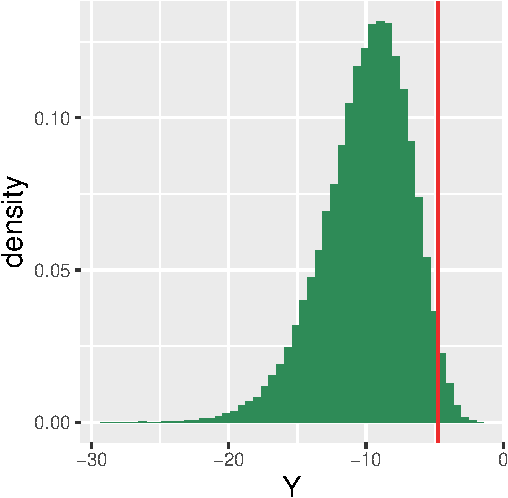
\includegraphics[keepaspectratio]{03-binomial_files/figure-latex/fig-cisim-1.pdf}}

}

\caption{\label{fig-cisim}The empirical sampling distribution for the
statistic \(Y = \sum_{i=1}^n \log X_i\), determined by simulating
100,000 datasets drawn from the distribution
\(f_X(x \vert \theta) = \theta x^{\theta-1}\). (Here, \(n = 10\) and
\(\theta = 1.75\).) The observed statistic value,
\(y_{\mathrm{obs}} = -4.758\), is indicated by the vertical red line,
and the estimated \(p\)-value is the proportion of simulation statistic
values falling to the right of the line.}

\end{figure}%

\begin{quote}
The estimated \(p\)-value is a point estimate. We can add value to this
estimate by using it to construct a confidence interval on the unknown
true \(p\)-value. We can do this because our simulation is like a
binomial experiment, in which
\end{quote}

\begin{quote}
\begin{enumerate}
\def\labelenumi{\arabic{enumi}.}
\tightlist
\item
  the number of trials \(k\) is the number of simulations
  (\texttt{num.sim}); and
\item
  the probability of success \(p\) is the probability of sampling a
  value of \(Y \geq y_{\mathrm{obs}}\) (given that this is an upper-tail
  test with \(E[Y]\) increasing with \(\theta\)).
\end{enumerate}
\end{quote}

\begin{quote}
In the code below, we denote the observed statistic (here, the number of
times we observe \(Y \geq y_{\mathrm{obs}}\)) as \texttt{u.obs}.
\end{quote}

\begin{Shaded}
\begin{Highlighting}[]
\NormalTok{alpha }\OtherTok{\textless{}{-}} \FloatTok{0.05}

\NormalTok{f }\OtherTok{\textless{}{-}} \ControlFlowTok{function}\NormalTok{(p, k, u.obs, q)}
\NormalTok{\{}
  \FunctionTok{pbinom}\NormalTok{(u.obs, }\AttributeTok{size =}\NormalTok{ k, }\AttributeTok{prob =}\NormalTok{ p) }\SpecialCharTok{{-}}\NormalTok{ q}
\NormalTok{\}}

\FunctionTok{round}\NormalTok{(}\FunctionTok{uniroot}\NormalTok{(f, }\AttributeTok{interval =} \FunctionTok{c}\NormalTok{(}\DecValTok{0}\NormalTok{, }\DecValTok{1}\NormalTok{), }\AttributeTok{k =}\NormalTok{ num.sim, }
              \AttributeTok{u.obs =} \FunctionTok{sum}\NormalTok{(Y }\SpecialCharTok{\textgreater{}=}\NormalTok{ y.obs) }\SpecialCharTok{{-}} \DecValTok{1}\NormalTok{, }\AttributeTok{q =} \DecValTok{1} \SpecialCharTok{{-}}\NormalTok{ alpha }\SpecialCharTok{/} \DecValTok{2}\NormalTok{)}\SpecialCharTok{$}\NormalTok{root, }\DecValTok{3}\NormalTok{)}
\end{Highlighting}
\end{Shaded}

\begin{verbatim}
[1] 0.023
\end{verbatim}

\begin{Shaded}
\begin{Highlighting}[]
\FunctionTok{round}\NormalTok{(}\FunctionTok{uniroot}\NormalTok{(f, }\AttributeTok{interval =} \FunctionTok{c}\NormalTok{(}\DecValTok{0}\NormalTok{, }\DecValTok{1}\NormalTok{), }\AttributeTok{k =}\NormalTok{ num.sim,}
              \AttributeTok{u.obs =} \FunctionTok{sum}\NormalTok{(Y }\SpecialCharTok{\textgreater{}=}\NormalTok{ y.obs)    , }\AttributeTok{q =}\NormalTok{     alpha }\SpecialCharTok{/} \DecValTok{2}\NormalTok{)}\SpecialCharTok{$}\NormalTok{root, }\DecValTok{3}\NormalTok{)}
\end{Highlighting}
\end{Shaded}

\begin{verbatim}
[1] 0.025
\end{verbatim}

\begin{quote}
(Note how we apply a discreteness correction when computing the lower
bound.) Our estimated 95\% confidence interval for the true \(p\)-value
is {[}0.0232,0.0251{]}; we can feel ``confident'' when we decide, in
this situation, to reject the null hypothesis that
\(\theta = \theta_o = 1\).
\end{quote}

\subsubsection{NP Lemma: When Data Reduction is Not
Possible}\label{np-lemma-when-data-reduction-is-not-possible}

\begin{quote}
The logistic distribution, whose probability density function is
\begin{align*}
f_X(x \vert \mu) = \frac{\exp(\mu-x)}{[1+\exp(\mu-x)]^2}
\end{align*} for \(x \in (-\infty,\infty)\) and
\(\mu \in (-\infty,\infty)\), is \emph{not} a member of the exponential
family of distributions. This means that if we sample \(n\) iid data
according to this distribution, we cannot reduce them so as to define a
single-number sufficient statistic for \(\mu\). What we \emph{can} do,
however, is the following:
\end{quote}

\begin{quote}
\begin{itemize}
\tightlist
\item
  we can simulate a large number of datasets under the null hypothesis
  \(\mu = \mu_o\);
\item
  for each dataset, we can record \(\ell(\mu_o \vert \mathbf{x})\) and
  \(\ell(\mu_a \vert \mathbf{x})\), and the difference between the two
  (which is \(\log \lambda_{NP}\)); and
\item
  we can determine the \(\alpha^{\mathrm{th}}\) percentile of the
  distribution of \(\log \lambda_{NP}\) values.
\end{itemize}
\end{quote}

\begin{quote}
The \(\alpha^{\mathrm{th}}\) percentile is the rejection-region boundary
for the most powerful test of the simple hypotheses \(\mu = \mu_o\) and
\(\mu = \mu_a\). Note that because \(\mu_a\) must be specified to carry
out the simulations, what we define is \emph{not} a uniformly most
powerful test.
\end{quote}

\begin{quote}
Below, we determine the the \(p\)-value, rejection-region boundary, and
the test power for a situation in which we sample \(n = 10\) iid data
according to a logistic distribution for which \(\mu_o = 1\), with our
alternative hypothesis being \(\mu_a = 3\). (See
Figure~\ref{fig-lognp}.)
\end{quote}

\begin{Shaded}
\begin{Highlighting}[]
\CommentTok{\# generate data}
\FunctionTok{set.seed}\NormalTok{(}\DecValTok{36236}\NormalTok{)}
\NormalTok{alpha   }\OtherTok{\textless{}{-}} \FloatTok{0.05}
\NormalTok{num.sim }\OtherTok{\textless{}{-}} \DecValTok{100000}
\NormalTok{n       }\OtherTok{\textless{}{-}} \DecValTok{10}
\NormalTok{mu.o    }\OtherTok{\textless{}{-}} \DecValTok{1}
\NormalTok{mu.a    }\OtherTok{\textless{}{-}} \DecValTok{2}
\NormalTok{X       }\OtherTok{\textless{}{-}} \FunctionTok{matrix}\NormalTok{(}\FunctionTok{rlogis}\NormalTok{(n }\SpecialCharTok{*}\NormalTok{ num.sim, }\AttributeTok{location =}\NormalTok{ mu.o), }\AttributeTok{nrow =}\NormalTok{ num.sim)}

\NormalTok{f }\OtherTok{\textless{}{-}} \ControlFlowTok{function}\NormalTok{(x, mu.o)}
\NormalTok{\{}
  \FunctionTok{sum}\NormalTok{(}\FunctionTok{log}\NormalTok{(}\FunctionTok{dlogis}\NormalTok{(x, }\AttributeTok{location =}\NormalTok{ mu.o)))}
\NormalTok{\}}
\NormalTok{log.like.o     }\OtherTok{\textless{}{-}} \FunctionTok{apply}\NormalTok{(X, }\DecValTok{1}\NormalTok{, f, }\AttributeTok{mu.o =}\NormalTok{ mu.o)}
\NormalTok{log.like.a     }\OtherTok{\textless{}{-}} \FunctionTok{apply}\NormalTok{(X, }\DecValTok{1}\NormalTok{, f, }\AttributeTok{mu.o =}\NormalTok{ mu.a)}
\NormalTok{delta.log.like }\OtherTok{\textless{}{-}}\NormalTok{ log.like.o }\SpecialCharTok{{-}}\NormalTok{ log.like.a}

\CommentTok{\# The p{-}value for a dataset sampled under the null}
\NormalTok{X.obs              }\OtherTok{\textless{}{-}} \FunctionTok{rlogis}\NormalTok{(n, }\AttributeTok{location =}\NormalTok{ mu.o)}
\NormalTok{delta.log.like.obs }\OtherTok{\textless{}{-}} \FunctionTok{f}\NormalTok{(X, mu.o) }\SpecialCharTok{{-}} \FunctionTok{f}\NormalTok{(X, mu.a)}
\NormalTok{p                  }\OtherTok{\textless{}{-}} \FunctionTok{sum}\NormalTok{(delta.log.like }\SpecialCharTok{\textless{}=}\NormalTok{ delta.log.like.obs) }\SpecialCharTok{/}\NormalTok{ num.sim}
\FunctionTok{round}\NormalTok{(p, }\DecValTok{4}\NormalTok{)}
\end{Highlighting}
\end{Shaded}

\begin{verbatim}
[1] 1
\end{verbatim}

\begin{Shaded}
\begin{Highlighting}[]
\CommentTok{\# The rejection{-}region boundary}
\NormalTok{rr }\OtherTok{\textless{}{-}} \FunctionTok{quantile}\NormalTok{(delta.log.like, }\AttributeTok{probs =}\NormalTok{ alpha)}
\FunctionTok{round}\NormalTok{(rr, }\DecValTok{3}\NormalTok{)}
\end{Highlighting}
\end{Shaded}

\begin{verbatim}
    5% 
-1.362 
\end{verbatim}

\begin{Shaded}
\begin{Highlighting}[]
\CommentTok{\# The test power for mu = mu.a}
\NormalTok{X                }\OtherTok{\textless{}{-}} \FunctionTok{matrix}\NormalTok{(}\FunctionTok{rlogis}\NormalTok{(n }\SpecialCharTok{*}\NormalTok{ num.sim, }\AttributeTok{location =}\NormalTok{ mu.a), }\AttributeTok{nrow =}\NormalTok{ num.sim)}
\NormalTok{log.like.o.p     }\OtherTok{\textless{}{-}} \FunctionTok{apply}\NormalTok{(X, }\DecValTok{1}\NormalTok{, f, }\AttributeTok{mu.o =}\NormalTok{ mu.o)}
\NormalTok{log.like.a.p     }\OtherTok{\textless{}{-}} \FunctionTok{apply}\NormalTok{(X, }\DecValTok{1}\NormalTok{, f, }\AttributeTok{mu.o =}\NormalTok{ mu.a)}
\NormalTok{delta.log.like.p }\OtherTok{\textless{}{-}}\NormalTok{ log.like.o.p }\SpecialCharTok{{-}}\NormalTok{ log.like.a.p}
\NormalTok{power            }\OtherTok{\textless{}{-}} \FunctionTok{sum}\NormalTok{(delta.log.like.p }\SpecialCharTok{\textless{}}\NormalTok{ rr) }\SpecialCharTok{/}\NormalTok{ num.sim}
\FunctionTok{round}\NormalTok{(power, }\DecValTok{3}\NormalTok{)}
\end{Highlighting}
\end{Shaded}

\begin{verbatim}
[1] 0.568
\end{verbatim}

\begin{figure}

\centering{

\pandocbounded{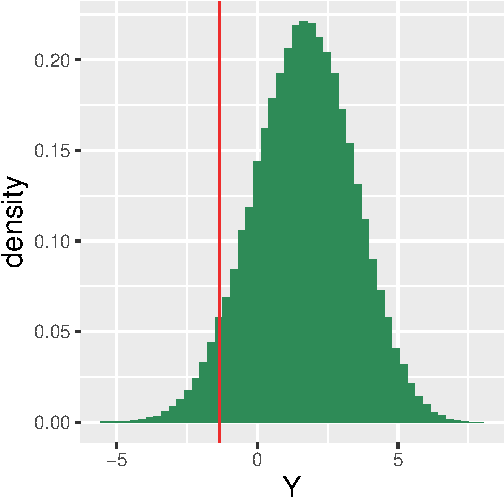
\includegraphics[keepaspectratio]{03-binomial_files/figure-latex/fig-lognp-1.pdf}}

}

\caption{\label{fig-lognp}The empirical sampling distribution for the
statistic \(Y = \log\lambda_{NP}\), determined by simulating 100,000
datasets of size \(n = 10\) drawn from a logistic distribution with mean
\(\mu_o = 1\). The estimated rejection-region boundary
\(\log c(\alpha)\) is indicated by the vertical red line; if the
\(y_{\mathrm{obs}} < \log c(\alpha)\) is less than the boundary value,
we would reject the null hypothesis that \(\mu_o = 1\).}

\end{figure}%

\subsubsection{Binomial Probability: Large-Sample Approximation
Tests}\label{binomial-probability-large-sample-approximation-tests}

\begin{quote}
In an example in Section~\ref{sec-chap3pmf}, we saw that if \[
k > 9\left(\frac{\mbox{max}(p,1-p)}{\mbox{min}(p,1-p)}\right) \,,
\] then, given a random variable \(X \sim\) Binomial(\(k\),\(p\)), we
can assume \[
X \overset{d}{\rightarrow} Y \sim \mathcal{N}(kp,kp(1-p)) \,,
\] or that \[
\hat{p} = \hat{p}_{MLE} = \frac{X}{k} \overset{d}{\rightarrow} X' \sim \mathcal{N}(p,p(1-p)/k) \,.
\] In hypothesis testing, this approximation forms the basis of two
different tests: \begin{align*}
\mbox{Score}~\mbox{Test:} ~~ & \hat{p} \sim \mathcal{N}(p_o,p_o(1-p_o)/k) \\
\mbox{Wald}~\mbox{Test:} ~~ & \hat{p} \sim \mathcal{N}(p_o,\hat{p}(1-\hat{p})/k) \,.
\end{align*} The only difference between the two is in how the variance
is estimated under the null. To carry out these tests, we can simply
adapt the expressions for the \(p\)-values, rejection regions, and power
so that we carry out carry out tests of the normal population mean with
\emph{variance known}, with the primary change being the definition of
the variance.
\end{quote}

\begin{quote}
We are including the details of the Wald and Score tests here for
completeness, in that they are ubiquitous in introductory statistics
settings. As they yield only approximate results, we would encourage the
reader to always use the exact testing mechanisms described previously,
while being mindful of the effects of the discreteness of the
probability mass function, especially when \(n\) and \(k\) are both
small.
\end{quote}

\subsubsection{Uniform Distribution: Test of Population Bound with
Sample
Median}\label{uniform-distribution-test-of-population-bound-with-sample-median}

\begin{quote}
Let's assume that we draw \(n\) iid data, where \(n\) is an odd number,
from a Uniform(\(0,\theta\)) distribution, and that we wish to test the
hypothesis \(H_o: \mu = \mu_o
= 1/2\) versus \(H_a: \mu = \mu_a > \mu_o\) at level \(\alpha\). (Let's
also assume that all the data we observe lie in the range
\([0,1]\)\ldots otherwise the null cannot be correct. We will return to
this point in Chapter~\ref{sec-chap5}.) Here we will show how to carry
out this test using the sample median as the test statistic. To be
clear, because the sample median is not a sufficient statistic for
\(\theta\), what we define here will not be a most powerful test.
\end{quote}

\begin{quote}
In Section~\ref{sec-chap3order}, we wrote down the formula for the order
statistic cdf: \[
F_{(j)}(x) = \sum_{i=j}^n \binom{n}{i} [F_X(x)]^i [1 - F_X(x)]^{n-i} \,. 
\] For the Uniform(\(0,\theta\)) distribution, the cdf is \[
F_X(x) = \int_0^x \frac{1}{\theta} dy = \frac{x}{\theta} \,,
\] and so the cdf for the sample median will be \[
F_{((n+1)/2)}(x) = \sum_{i=(n+1)/2}^n \binom{n}{i} \left[\frac{x}{\theta}\right]^i \left[1 - \frac{x}{\theta}\right]^{n-i} \,. 
\] This is easily coded. Let's do this, assuming that, e.g., \(n = 11\)
and the observed median value is
\(y_{\mathrm{obs}} = \tilde{x}_{\mathrm{obs}} = 0.61\). Note that
because \(E[Y]\) increases with \(\theta\), then the \(p\)-value for
this test will be
\(1 - F_{((n+1)/2)}(\tilde{x}_{\mathrm{obs}} \vert \theta_o)\).
\end{quote}

\begin{Shaded}
\begin{Highlighting}[]
\NormalTok{F }\OtherTok{\textless{}{-}} \ControlFlowTok{function}\NormalTok{(x, j, n, theta)}
\NormalTok{\{}
\NormalTok{  i }\OtherTok{\textless{}{-}}\NormalTok{ j}\SpecialCharTok{:}\NormalTok{n}
  \FunctionTok{sum}\NormalTok{( }\FunctionTok{choose}\NormalTok{(n, i) }\SpecialCharTok{*}\NormalTok{ (x }\SpecialCharTok{/}\NormalTok{ theta)}\SpecialCharTok{\^{}}\NormalTok{i }\SpecialCharTok{*}\NormalTok{ (}\DecValTok{1} \SpecialCharTok{{-}}\NormalTok{ x }\SpecialCharTok{/}\NormalTok{ theta)}\SpecialCharTok{\^{}}\NormalTok{(n }\SpecialCharTok{{-}}\NormalTok{ i) ) }
\NormalTok{\}}

\NormalTok{y.obs   }\OtherTok{\textless{}{-}} \FloatTok{0.61}
\NormalTok{n       }\OtherTok{\textless{}{-}} \DecValTok{11}
\NormalTok{j       }\OtherTok{\textless{}{-}} \DecValTok{6}
\NormalTok{theta.o }\OtherTok{\textless{}{-}} \DecValTok{1}
\FunctionTok{round}\NormalTok{(}\DecValTok{1} \SpecialCharTok{{-}} \FunctionTok{F}\NormalTok{(y.obs, j, n, theta.o), }\DecValTok{3}\NormalTok{)}
\end{Highlighting}
\end{Shaded}

\begin{verbatim}
[1] 0.225
\end{verbatim}

\begin{quote}
The observed \(p\)-value is 0.225; we fail to reject the null hypothesis
and conclude that we have insufficient statistical evidence to rule out
that \(\theta = 1\).
\end{quote}

\section{Hypothesis Testing: Categorical
Hypotheses}\label{sec-chap3categorical}

What to take away from this section:

\begin{itemize}
\item
  Conducting, e.g., surveys and observational studies can lead to the
  generation of multinomially distributed data, i.e., data that are
  recorded across a set of ``bins.''
\item
  Given a single vector of multinomial data \(\{X_1,\ldots,X_m\}\),
  where \(\sum_{i=1}^m X_i = k\), and a null hypothesis that the
  expected data proportions across the bins are
  \(\{p_{1,o},\ldots,p_{m,o}\}\), we should carry out \emph{multinomial
  simulations} so as to derive exact hypothesis test \(p\)-values, as
  opposed to the historically often-used \emph{chi-square
  goodness-of-fit} test.
\item
  If our data are arrayed across a \emph{contingency table} with \(r\)
  rows and \(c\) columns, there are a number of hypothesis tests that
  one could conceivably carry out, including \emph{Barnard's exact
  test}, the \emph{chi-square test of homogeneity}, and the
  \emph{chi-square test of independence}.
\end{itemize}

For previous material on hypothesis testing, see
Section~\ref{sec-chap2hypothesis}.

In Section~\ref{sec-chap3nplemma}, we expanded upon our descriptions of
hypothesis testing given earlier in the book by showing how the
Neyman-Pearson lemma allows us to define, e.g., uniformly most powerful
one-tail hypothesis tests for the values of parameters of members of the
exponential family of distributions. However, with the introduction of
categorical data in this chapter, data that we can model with binomial
or multinomial distributions, there is a new aspect to hypothesis
testing that we will begin to discuss here: testing \emph{categorical
hypotheses}.

Let's begin by making up a simple dataset:

{\def\LTcaptype{none} % do not increment counter
\begin{longtable}[]{@{}cccc@{}}
\toprule\noalign{}
\endhead
\bottomrule\noalign{}
\endlastfoot
\(x_1\) & \(x_2\) & \(x_3\) & \(n = \sum_{i=1}^3 x_i\) \\
6 & 10 & 4 & 20 \\
\end{longtable}
}

In this experiment, \(n = 20\) data were collected, with three possible
outcomes: \(\{X_1, X_2, X_3\}\).

\subsection{Multinomial Simulations}\label{sec-chap3multisim}

Assuming that \(n\) was fixed prior to data collection, this is an
example of a \emph{multinomial experiment}. (We defer discussion of how
subsequent testing changes if \(n\) is not fixed to
Section~\ref{sec-chap4hypothesis}.) This data vector is trivially a
sufficient statistic for the vector of probabilities
\(\mathbf{p} = \{p_1, p_2 ,p_3\}\), and the probability mass function of
the sampling distribution for this statistic is simply the multinomial
pmf introduced in Section~\ref{sec-chap3multi}.

It is natural, given such data, to test whether or not they are
consistent with a specified probability vector:
\(\mathbf{p}_o = \{p_{1,o}, p_{2,o} ,p_{3,o}\}\). This is our null
hypothesis; the alternative is that at least two of the probabilities
differ from the specified values. As we cannot carry out the test by
hand, we fall back on the definition of a \(p\)-value and use
simulations to estimate the proportion of data vectors simulated under
the null hypothesis that have pmf values that are smaller than what we
observe. Such simulations are straightforward, as we show in an example
below.

\subsection{The Chi-Square Goodness-of-Fit Test}\label{sec-chap3gof}

We note that in the era before computers, statisticians could not carry
out such simulations. In Pearson (1900), it was noted that as
\(k \rightarrow \infty\), multinomial random variables converge in
distribution to multivariate normal random variables (with the
multivariate normal being something we will discuss in
Section~\ref{sec-chap6multnorm}), and that the statistic \[
W = \sum_{i=1}^m \frac{(X_i-E[X_i])^2}{E[X_i]} = \sum_{i=1}^m \frac{(X_i - kp_i)^2}{kp_i}
\] converges in distribution to a chi-square random variable for \(m-1\)
degrees of freedom. (We subtract 1 because only \(m-1\) of the
multinomial probabilities can freely vary; the \(m^{th}\) one is
constrained by the fact that the probabilities must sum to 1. This
constraint is what makes multinomial data \emph{not} iid.) In another
example below, we show how one can use the \emph{chi-square
goodness-of-fit test} in place of multinomial simulations. However, we
will state here that because the chi-square GoF test is based on a
large-sample approximation, any computed \(p\)-value will only be
approximately correct. Given the choice, \textbf{one should always
implement exact multinomial tests rather than approximate chi-square GoF
tests}. In an example below, we demonstrate that the chi-square GoF test
yields \(p\)-values that are, on average, smaller than expected, making
it less conservative than the exact multinomial test (i.e., it rejects
correct null hypotheses at a higher rate than we would expect).

\subsection{The Chi-Square Tests of Independence and
Homogeneity}\label{sec-chap3indhom}

Let's build upon the simple dataset shown above, by adding another row
of data:

{\def\LTcaptype{none} % do not increment counter
\begin{longtable}[]{@{}ccccc@{}}
\toprule\noalign{}
\endhead
\bottomrule\noalign{}
\endlastfoot
& \(x_1\) & \(x_2\) & \(x_3\) & \(\sum_{i=1}^3 x_i\) \\
\(y_1\) & 6 & 10 & 4 & 20 \\
\(y_2\) & 8 & 4 & 8 & 20 \\
\(\sum_{i=1}^2 y_i\) & 14 & 14 & 12 & 40 \\
\end{longtable}
}

The experiment that generated these data had six possible outcomes, and
we display the data in a \(2 \times 3\) \emph{contingency table}. (To be
clear, there is nothing special here about the exact number of rows or
columns\ldots the key is that we have more than one of each.) Given such
data, the typical question of interest is whether the data in each row
(or, equivalently, in each column) are sampled from the same
distribution. Generally, that question is to be answered without regard
to the actual probabilities that we would observe each outcome; i.e.,
the null hypothesis is simply that the vectors of probabilities in each
row (or, equivalently, in each column) are the same. Because the null
hypothesis probabilities are implicitly estimated and not explicitly
specified, one cannot test the null using multinomial simulations. There
is a variety of tests that one can apply; which is the optimal choice
depends on the details of the experimental design.

\begin{enumerate}
\def\labelenumi{\arabic{enumi}.}
\item
  \emph{The data are displayed in a \(2 \times 2\) contingency table,
  with the row and column sums both fixed by design.} In such a
  situation, we might use \emph{Fisher's exact test}. However, such
  designs are rare and Fisher's test, as constructed, is generally too
  conservative (i.e., it produces \(p\)-values that are larger than they
  should be), so we will forgo discussing Fisher's test further here.
\item
  \emph{The data are displayed in a \(2 \times 2\) contingency table,
  with either the row sums or the column sums fixed by design (but not
  both).} Here, we would use, e.g., a test related to \emph{Barnard's
  exact test}, which is effectively a two-sample test of binomial
  proportions.
\item
  \emph{The data are displayed in a contingency table that is larger
  than \(2 \times 2\), with either the row sums or the column sums fixed
  by design (but not both).} Here, we would apply the \emph{chi-square
  test of homogeneity}.
\item
  \emph{The data are displayed in a contingency table that is larger
  than \(2 \times 2\), with neither the row sums nor the column sums
  fixed by design.} Here, we would apply the \emph{chi-square test of
  independence}.
\end{enumerate}

As we will see, the mathematical details for the chi-square tests of
homogeneity and independence are identical, and thus both are
demonstrated within a single example below.

\subsection{Examples}\label{examples-34}

\subsubsection{Multinomial Simulations}\label{multinomial-simulations}

\begin{quote}
Imagine that we are scientists, sitting on a platform in the middle of a
plain, and we have decided that we will record the azimuthal angle for
each of the first \(k = 100\) animals we observe. (An azimuthal angle
is, e.g., \(0^\circ\) when looking directly north, and 90\(^\circ\),
180\(^\circ\), and 270\(^\circ\) as we look east, south, and west, etc.)
These are our data:
\end{quote}

{\def\LTcaptype{none} % do not increment counter
\begin{longtable}[]{@{}
  >{\centering\arraybackslash}p{(\linewidth - 10\tabcolsep) * \real{0.3023}}
  >{\centering\arraybackslash}p{(\linewidth - 10\tabcolsep) * \real{0.1395}}
  >{\centering\arraybackslash}p{(\linewidth - 10\tabcolsep) * \real{0.1395}}
  >{\centering\arraybackslash}p{(\linewidth - 10\tabcolsep) * \real{0.1395}}
  >{\centering\arraybackslash}p{(\linewidth - 10\tabcolsep) * \real{0.1395}}
  >{\centering\arraybackslash}p{(\linewidth - 10\tabcolsep) * \real{0.1395}}@{}}
\toprule\noalign{}
\endhead
\bottomrule\noalign{}
\endlastfoot
angle range & 0\(^\circ\)-90\(^\circ\) & 90\(^\circ\)-180\(^\circ\) &
180\(^\circ\)-270\(^\circ\) & 270\(^\circ\)-360\(^\circ\) & \\
number of animals & 28 & 32 & 17 & 23 & 100 \\
\end{longtable}
}

\begin{quote}
The question we wish to answer is whether the animals are uniformly
distributed across all four quadrants.
\end{quote}

\begin{quote}
These data are multinomial data: the number of trials is fixed, and
there are four possible outcomes for each. To answer the question, then,
we simulate \(100{,}000\) data vectors given the null hypothesis
\(H_o : \{p_1 = 0.25, p_2 = 0.25, p_3 = 0.25, p_4 = 0.25\}\) and
determine the proportion of vectors with multinomial pmf values that are
smaller than the value we observe:
\end{quote}

\begin{Shaded}
\begin{Highlighting}[]
\NormalTok{O       }\OtherTok{\textless{}{-}} \FunctionTok{c}\NormalTok{(}\DecValTok{28}\NormalTok{, }\DecValTok{32}\NormalTok{, }\DecValTok{17}\NormalTok{, }\DecValTok{23}\NormalTok{)}
\NormalTok{p       }\OtherTok{\textless{}{-}} \FunctionTok{rep}\NormalTok{(}\DecValTok{1}\SpecialCharTok{/}\DecValTok{4}\NormalTok{, }\DecValTok{4}\NormalTok{)}
\NormalTok{pmf.obs }\OtherTok{\textless{}{-}} \FunctionTok{dmultinom}\NormalTok{(O, }\AttributeTok{prob =}\NormalTok{ p)       }\CommentTok{\# the observed multinomial pmf value}

\FunctionTok{set.seed}\NormalTok{(}\DecValTok{101}\NormalTok{)}

\NormalTok{num.sim }\OtherTok{\textless{}{-}} \DecValTok{100000}
\NormalTok{k       }\OtherTok{\textless{}{-}} \FunctionTok{sum}\NormalTok{(O)}
\NormalTok{m       }\OtherTok{\textless{}{-}} \FunctionTok{length}\NormalTok{(O)}
\NormalTok{X       }\OtherTok{\textless{}{-}} \FunctionTok{rmultinom}\NormalTok{(num.sim, k, p)     }\CommentTok{\# generates an m x num.sim matrix}
                                        \CommentTok{\# (m determined as the length of p)}
\NormalTok{pmf     }\OtherTok{\textless{}{-}} \FunctionTok{apply}\NormalTok{(X, }\DecValTok{2}\NormalTok{, }\ControlFlowTok{function}\NormalTok{(x)\{}\FunctionTok{dmultinom}\NormalTok{(x, }\AttributeTok{prob =}\NormalTok{ p)\}) }\CommentTok{\# pmf vector}
\FunctionTok{round}\NormalTok{(}\FunctionTok{sum}\NormalTok{(pmf }\SpecialCharTok{\textless{}}\NormalTok{ pmf.obs) }\SpecialCharTok{/}\NormalTok{ num.sim, }\DecValTok{4}\NormalTok{)  }\CommentTok{\# the estimated p{-}value}
\end{Highlighting}
\end{Shaded}

\begin{verbatim}
[1] 0.1597
\end{verbatim}

\begin{quote}
What does \texttt{apply()} do? It calls the function given as the third
argument (which evaluates the multinomial probability mass function
given a set of four data \(\mathbf{x}\) and a a set of four
probabilities \(\mathbf{p}\)) to each \emph{column} (hence the ``2'' as
the second argument\ldots{}``1'' would denote rows) of the matrix
\(\mathbf{X}\). It is a convenient function that allows us to not have
to embed the evaluation of the multinomial pmf into a \texttt{for} loop
that would iterate over all the rows of the matrix. We note that the
above computation takes \(\sim\) 1 CPU second on a standard
desktop/laptop computer.
\end{quote}

\begin{quote}
We observe \(p = 0.1597\), i.e., approximately \(16{,}000\) of the
\(100{,}000\) simulated data vectors have pmf values smaller than what
we observe. We thus fail to reject the null hypothesis and conclude that
it is plausible that the animals are distributed uniformly as a function
of angle.
\end{quote}

\begin{quote}
The multinomial hypothesis test is ``exact,'' in the sense that the data
are distributed according to the multinomial distribution, but because
we only sample a finite number of data vectors, the \(p\)-value is only
an estimate and not an exact value. We can utilize the framework given
earlier, in Section~\ref{sec-chap3confidence}, to construct a 95\%
confidence interval for the binomial probability \(p\), given our
simulation result:
\end{quote}

\begin{Shaded}
\begin{Highlighting}[]
\NormalTok{alpha }\OtherTok{\textless{}{-}} \FloatTok{0.05}
\NormalTok{Y     }\OtherTok{\textless{}{-}} \FunctionTok{sum}\NormalTok{(pmf }\SpecialCharTok{\textless{}}\NormalTok{ pmf.obs)}

\NormalTok{f }\OtherTok{\textless{}{-}} \ControlFlowTok{function}\NormalTok{(p, k, y.obs, q)}
\NormalTok{\{}
  \FunctionTok{pbinom}\NormalTok{(y.obs, }\AttributeTok{size =}\NormalTok{ k, }\AttributeTok{prob =}\NormalTok{ p) }\SpecialCharTok{{-}}\NormalTok{ q}
\NormalTok{\}}

\FunctionTok{round}\NormalTok{(}\FunctionTok{uniroot}\NormalTok{(f, }\AttributeTok{interval =} \FunctionTok{c}\NormalTok{(}\DecValTok{0}\NormalTok{, }\DecValTok{1}\NormalTok{), }\AttributeTok{k =}\NormalTok{ num.sim,}
              \AttributeTok{y.obs =}\NormalTok{ Y }\SpecialCharTok{{-}} \DecValTok{1}\NormalTok{, }\AttributeTok{q =} \DecValTok{1} \SpecialCharTok{{-}}\NormalTok{ alpha }\SpecialCharTok{/} \DecValTok{2}\NormalTok{)}\SpecialCharTok{$}\NormalTok{root, }\DecValTok{4}\NormalTok{)}
\end{Highlighting}
\end{Shaded}

\begin{verbatim}
[1] 0.1574
\end{verbatim}

\begin{Shaded}
\begin{Highlighting}[]
\FunctionTok{round}\NormalTok{(}\FunctionTok{uniroot}\NormalTok{(f, }\AttributeTok{interval =} \FunctionTok{c}\NormalTok{(}\DecValTok{0}\NormalTok{, }\DecValTok{1}\NormalTok{), }\AttributeTok{k =}\NormalTok{ num.sim,}
              \AttributeTok{y.obs =}\NormalTok{ Y,     }\AttributeTok{q =}\NormalTok{     alpha }\SpecialCharTok{/} \DecValTok{2}\NormalTok{)}\SpecialCharTok{$}\NormalTok{root, }\DecValTok{4}\NormalTok{)}
\end{Highlighting}
\end{Shaded}

\begin{verbatim}
[1] 0.162
\end{verbatim}

\begin{quote}
The 95\% two-sided confidence interval on the true \(p\)-value is
\([0.1574,0.1620]\): when we fail to reject the null, we can be very
confident that we are not making a mistake. To decrease the interval
length, we would simply increase \texttt{num.sim}; the tradeoff is that
the computation time becomes that much longer.
\end{quote}

\subsubsection{Chi-Square Goodness of Fit
Test}\label{chi-square-goodness-of-fit-test}

\begin{quote}
The computation of the test statistic \(W\) is the basis of the
\emph{chi-square goodness-of-fit test}, or chi-square GoF test. For this
test,
\end{quote}

\begin{quote}
\begin{itemize}
\tightlist
\item
  we reject the null hypothesis if \(W > w_{RR}\);
\item
  the \(p\)-value is \(1 - F_{W(m-1)}(w_{\mathrm{obs}})\) (e.g.,
  \texttt{1\ -\ pchisq(w.obs,\ m\ -\ 1)}); and
\item
  by convention, \(kp_i\) must be \(\geq\) 5 in each bin for the test to
  yield a valid result.
\end{itemize}
\end{quote}

\begin{quote}
We are discussing the chi-square GoF test here because its use is
ubiquitous in statistics and thus every student should know what it is
and how it is carried out\ldots but not because one should actually use
it now, in the age of computers. The price that we pay when we use the
chi-square GoF test is that, for relatively small values of \(k\), it
yields \emph{biased} \(p\)-value estimates.
\end{quote}

\begin{quote}
Let's go back to working with our animal/angle data, and determine, via
the use of the chi-square GoF test, whether it is plausible that the
number of animals is distributed uniformly as a function of angle.
\end{quote}

\begin{quote}
We first compute the test statistic: \begin{align*}
W &= \sum_{i=1}^m \frac{(X_i - kp_i)^2}{kp_i} \\
&= \frac{(28-25)^2}{25} + \frac{(32-25)^2}{25} + \frac{(17-25)^2}{25} + \frac{(23-25)^2}{25} \\
&= \frac{9}{25} + \frac{49}{25} + \frac{64}{25} + \frac{4}{25} = \frac{126}{25} = 5.04 \,.
\end{align*} The number of degrees of freedom is \(m-1 = 3\), so the
\(p\)-value is
\end{quote}

\begin{Shaded}
\begin{Highlighting}[]
\NormalTok{W }\OtherTok{\textless{}{-}} \FunctionTok{sum}\NormalTok{( (O }\SpecialCharTok{{-}}\NormalTok{ k }\SpecialCharTok{*}\NormalTok{ p)}\SpecialCharTok{\^{}}\DecValTok{2} \SpecialCharTok{/}\NormalTok{ (k }\SpecialCharTok{*}\NormalTok{ p) )}
\FunctionTok{round}\NormalTok{(}\DecValTok{1} \SpecialCharTok{{-}} \FunctionTok{pchisq}\NormalTok{(W, m }\SpecialCharTok{{-}} \DecValTok{1}\NormalTok{), }\DecValTok{3}\NormalTok{)}
\end{Highlighting}
\end{Shaded}

\begin{verbatim}
[1] 0.169
\end{verbatim}

\begin{quote}
We fail to reject the null hypothesis that the animals are distributed
uniformly as a function of azimuthal angle. See
Figure~\ref{fig-chi2gof}.
\end{quote}

\begin{figure}

\centering{

\pandocbounded{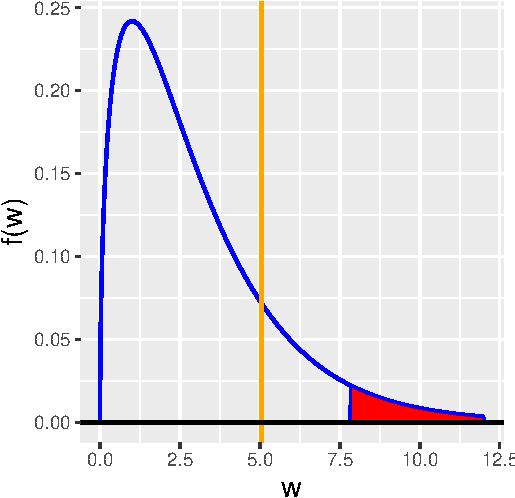
\includegraphics[keepaspectratio]{03-binomial_files/figure-latex/fig-chi2gof-1.pdf}}

}

\caption{\label{fig-chi2gof}An illustration of the sampling distribution
and rejection region for the chi-square goodness-of-fit test. Here, the
number of degrees of freedom is 3, so the rejection region are values of
chi-square above 7.815. The observed test statistic is 5.04, which lies
outside the rejection region, hence we fail to reject the null
hypothesis.}

\end{figure}%

\begin{quote}
The observed \(p\)-value, 0.169, is 5.6\% larger than the value observed
for the exact multinomial test (0.160, with 95\% CI \([0.1574,0.1620]\)
for \(100{,}000\) simulations). As we will see below, sometimes the
\(p\)-value is larger and sometimes smaller, but on average the
\(p\)-value observed for the chi-square GoF test will be \emph{smaller}
than that observed for the multinomial test, at least for small values
of \(k\). We elaborate on this point in the next example below.
\end{quote}

\subsubsection{Comparing Multinomial Simulations with the Chi-Square GoF
Test}\label{comparing-multinomial-simulations-with-the-chi-square-gof-test}

\begin{quote}
Let's suppose that in an experiment, we toss a six-sided die \(k\) times
and record the result. For instance, we might toss it \(k = 10\) times,
and record the data vector \(\mathbf{X} = \{2,1,3,1,0,3\}\) (i.e., we
observe 1 two times, 2 one time, etc.). We wish to test the hypothesis
that the die is fair. On average, what is the difference in the
\(p\)-value observed when utilize the exact multinomial test versus when
we utilize the approximate chi-square GoF test?
\end{quote}

\begin{quote}
Let's first illustrate how we would determine the average difference
when \(k = 30\). (See Figure~\ref{fig-deltap}.) For this number of
trials, the expected number of counts in each bin is exactly 5, i.e.,
this is the minimum number of trials required by convention when
carrying out the chi-square GoF test.
\end{quote}

\begin{Shaded}
\begin{Highlighting}[]
\NormalTok{k }\OtherTok{\textless{}{-}} \DecValTok{30}
\NormalTok{m }\OtherTok{\textless{}{-}} \DecValTok{6}
\NormalTok{p }\OtherTok{\textless{}{-}} \FunctionTok{rep}\NormalTok{(}\DecValTok{1} \SpecialCharTok{/}\NormalTok{ m, m)}

\FunctionTok{set.seed}\NormalTok{(}\DecValTok{101}\NormalTok{)}

\NormalTok{num.rep }\OtherTok{\textless{}{-}} \DecValTok{1000}
\NormalTok{p.chi   }\OtherTok{\textless{}{-}} \FunctionTok{rep}\NormalTok{(}\ConstantTok{NA}\NormalTok{, num.rep)}
\NormalTok{p.mult  }\OtherTok{\textless{}{-}} \FunctionTok{rep}\NormalTok{(}\ConstantTok{NA}\NormalTok{, num.rep)}
\NormalTok{delta.p }\OtherTok{\textless{}{-}} \FunctionTok{rep}\NormalTok{(}\ConstantTok{NA}\NormalTok{, num.rep)}

\NormalTok{num.sim }\OtherTok{\textless{}{-}} \DecValTok{1000}
\ControlFlowTok{for}\NormalTok{ ( ii }\ControlFlowTok{in} \DecValTok{1}\SpecialCharTok{:}\NormalTok{num.rep ) \{}
\NormalTok{  X.obs       }\OtherTok{\textless{}{-}} \FunctionTok{rmultinom}\NormalTok{(}\DecValTok{1}\NormalTok{, k, p)}
\NormalTok{  W           }\OtherTok{\textless{}{-}} \FunctionTok{sum}\NormalTok{((X.obs }\SpecialCharTok{{-}}\NormalTok{ k }\SpecialCharTok{*}\NormalTok{ p)}\SpecialCharTok{\^{}}\DecValTok{2} \SpecialCharTok{/}\NormalTok{ (k }\SpecialCharTok{*}\NormalTok{ p))}
\NormalTok{  p.chi[ii]   }\OtherTok{\textless{}{-}} \DecValTok{1} \SpecialCharTok{{-}} \FunctionTok{pchisq}\NormalTok{(W, m }\SpecialCharTok{{-}} \DecValTok{1}\NormalTok{)}
\NormalTok{  obs         }\OtherTok{\textless{}{-}} \FunctionTok{dmultinom}\NormalTok{(X.obs, }\AttributeTok{prob =}\NormalTok{ p)}
\NormalTok{  X           }\OtherTok{\textless{}{-}} \FunctionTok{rmultinom}\NormalTok{(num.sim, k, p)}
\NormalTok{  a           }\OtherTok{\textless{}{-}} \FunctionTok{apply}\NormalTok{(X, }\DecValTok{2}\NormalTok{, }\ControlFlowTok{function}\NormalTok{(x, p)\{}\FunctionTok{dmultinom}\NormalTok{(x, }\AttributeTok{prob =}\NormalTok{ p)\}, }\AttributeTok{p =}\NormalTok{ p)}
\NormalTok{  p.mult[ii]  }\OtherTok{\textless{}{-}} \FunctionTok{sum}\NormalTok{(a }\SpecialCharTok{\textless{}=}\NormalTok{ obs) }\SpecialCharTok{/}\NormalTok{ num.sim}
\NormalTok{  delta.p[ii] }\OtherTok{\textless{}{-}}\NormalTok{ p.mult[ii] }\SpecialCharTok{{-}}\NormalTok{ p.chi[ii]}
\NormalTok{\}}

\FunctionTok{cat}\NormalTok{(}\StringTok{"Mean Difference:"}\NormalTok{,}\FunctionTok{round}\NormalTok{(}\FunctionTok{mean}\NormalTok{(delta.p), }\DecValTok{5}\NormalTok{), }\StringTok{"}\SpecialCharTok{\textbackslash{}n}\StringTok{"}\NormalTok{)}
\end{Highlighting}
\end{Shaded}

\begin{verbatim}
Mean Difference: 0.0108 
\end{verbatim}

\begin{Shaded}
\begin{Highlighting}[]
\FunctionTok{cat}\NormalTok{(}\StringTok{"SE Difference:  "}\NormalTok{,}\FunctionTok{round}\NormalTok{(}\FunctionTok{sd}\NormalTok{(delta.p) }\SpecialCharTok{/} \FunctionTok{sqrt}\NormalTok{(num.rep), }\DecValTok{5}\NormalTok{), }\StringTok{"}\SpecialCharTok{\textbackslash{}n\textbackslash{}n}\StringTok{"}\NormalTok{)}
\end{Highlighting}
\end{Shaded}

\begin{verbatim}
SE Difference:   0.00135 
\end{verbatim}

\begin{figure}

\centering{

\pandocbounded{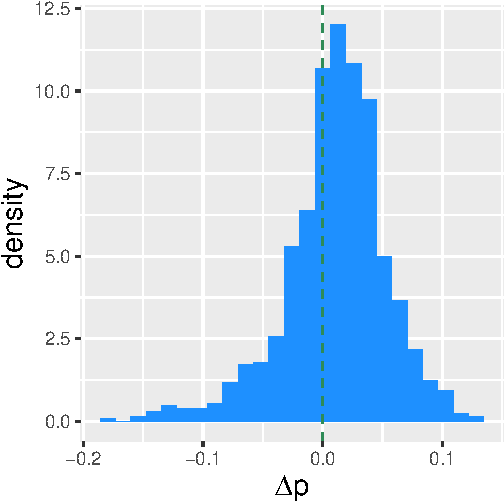
\includegraphics[keepaspectratio]{03-binomial_files/figure-latex/fig-deltap-1.pdf}}

}

\caption{\label{fig-deltap}Histogram showing the empirical distribution
of values of \(\Delta p = p_{\mathrm{mult}} - p_{\mathrm{chi}}\) that
arise when we repeatedly toss a die 30 times and test whether the die is
fair. If \(\Delta p > 0\), then the chi-square test is less
conservative, i.e., we are more likely to reject a correct null than if
we are to use the exact multinomial test. Here, the average value of
\(\Delta p\) is \(\approx 0.01\).}

\end{figure}%

\begin{quote}
We find that for \(k = 30\), the average value of
\(\Delta p = p_{\mathrm{mult}} - p_{\mathrm{chi}}\) is \(\approx 0.01\),
i.e., on average the chi-square GoF test is less conservative (or more
likely to result in the rejection of a correct null hypothesis).
\end{quote}

\begin{quote}
In Figure~\ref{fig-deltap2}, we show how the average value of
\(\Delta p\) changes as a function of \(k\). We see here that while by
convention the expected number of counts per bin is supposed to be at
least five, it is only when the expected counts reach \(\approx\) 20 or
more that we no longer observed a statistically significant difference
between the average \(p\)-values.
\end{quote}

\begin{figure}

\centering{

\pandocbounded{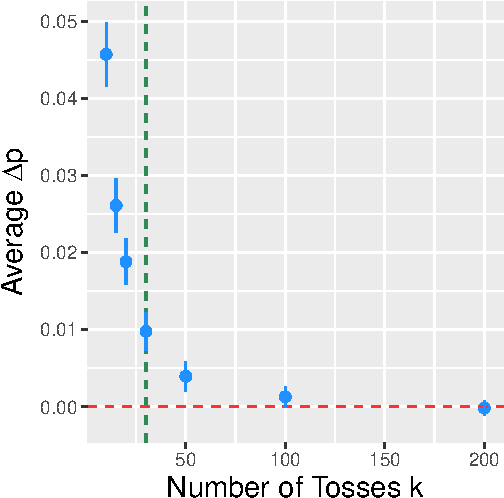
\includegraphics[keepaspectratio]{03-binomial_files/figure-latex/fig-deltap2-1.pdf}}

}

\caption{\label{fig-deltap2}The average value of
\(\Delta p = p_{\mathrm{mult}} - p_{\mathrm{chi}}\) as a function of the
number of tosses of a six-sided die. The vertical dashed green line at
\(k = 30\) represents where the expected number of counts in each data
bin is exactly 5, the minimum value conventionally required for use of
the chi-square GoF test.}

\end{figure}%

\subsubsection{Chi-Square GoF Test: Discrete
Distributions}\label{chi-square-gof-test-discrete-distributions}

\begin{quote}
In Section~\ref{sec-chap2distribution}, we introduced the
Kolmogorov-Smirnov test, which one can use to test the null hypothesis
that a set of data are sampled according to a specified continuous
distribution. How, on the other hand, might we determine whether a set
of data are sampled according to a specified \emph{discrete
distribution}?
\end{quote}

\begin{quote}
The chi-square goodness-of-fit test is a mechanism for doing just that.
Let's illustrate its use via an example.
\end{quote}

\begin{quote}
In a survey, 100 people were presented with a list of four restaurants
and asked to indicate how many they had eaten at. These are the data:
\end{quote}

{\def\LTcaptype{none} % do not increment counter
\begin{longtable}[]{@{}ccccc@{}}
\toprule\noalign{}
\endhead
\bottomrule\noalign{}
\endlastfoot
0 & 1 & 2 & 3 & 4 \\
30 & 22 & 20 & 16 & 12 \\
\end{longtable}
}

\begin{quote}
Is it plausible that these data are sampled according to a binomial
distribution with \(k = 4\) and unknown success probability \(p\)?
\end{quote}

\begin{quote}
Key to this exercise is that we are not specifying \(p\). If we did
specify it, then we would be able to carry out multinomial simulations
(since we would know the pmf value for each bin)\ldots if the
\(p\)-value is less than 0.05, we would reject the null and conclude
that it is implausible that the data are sampled according to a
Binom(\(k,p\)) distribution.
\end{quote}

\begin{quote}
Carrying out the test is a two-step process. First, we must estimate
\(p\). We use the maximum-likelihood estimate, \(X_+/nk\): \[
\hat{p} = \frac{0 \cdot 30 + 1 \cdot 22 + 2 \cdot 20 + 3 \cdot 16 + 4 \cdot 12}{100 \cdot 4} = 0.395 \,.
\] We then apply that estimate within the chi-square GoF test framework:
\end{quote}

\begin{Shaded}
\begin{Highlighting}[]
\NormalTok{p.hat }\OtherTok{\textless{}{-}}\NormalTok{ (}\DecValTok{0} \SpecialCharTok{*} \DecValTok{30} \SpecialCharTok{+} \DecValTok{1} \SpecialCharTok{*} \DecValTok{22} \SpecialCharTok{+} \DecValTok{2} \SpecialCharTok{*} \DecValTok{20} \SpecialCharTok{+} \DecValTok{3} \SpecialCharTok{*} \DecValTok{16} \SpecialCharTok{+} \DecValTok{4} \SpecialCharTok{*} \DecValTok{12}\NormalTok{)}\SpecialCharTok{/}\NormalTok{(}\DecValTok{100} \SpecialCharTok{*} \DecValTok{4}\NormalTok{)}

\NormalTok{O }\OtherTok{\textless{}{-}} \FunctionTok{c}\NormalTok{(}\DecValTok{30}\NormalTok{, }\DecValTok{22}\NormalTok{, }\DecValTok{20}\NormalTok{, }\DecValTok{16}\NormalTok{, }\DecValTok{12}\NormalTok{)}
\NormalTok{E }\OtherTok{\textless{}{-}} \DecValTok{100} \SpecialCharTok{*} \FunctionTok{dbinom}\NormalTok{(}\DecValTok{0}\SpecialCharTok{:}\DecValTok{4}\NormalTok{, }\AttributeTok{size =} \FloatTok{2.5}\NormalTok{, }\AttributeTok{prob =}\NormalTok{ p.hat)}
\end{Highlighting}
\end{Shaded}

\begin{verbatim}
Warning in dbinom(0:4, size = 2.5, prob = p.hat): NaNs produced
\end{verbatim}

\begin{Shaded}
\begin{Highlighting}[]
\NormalTok{W }\OtherTok{\textless{}{-}} \FunctionTok{sum}\NormalTok{( (O }\SpecialCharTok{{-}}\NormalTok{ E)}\SpecialCharTok{\^{}}\DecValTok{2} \SpecialCharTok{/}\NormalTok{ E )}
\NormalTok{m }\OtherTok{\textless{}{-}} \FunctionTok{length}\NormalTok{(O)}
\FunctionTok{round}\NormalTok{(}\DecValTok{1} \SpecialCharTok{{-}} \FunctionTok{pchisq}\NormalTok{(W, m }\SpecialCharTok{{-}} \DecValTok{2}\NormalTok{), }\DecValTok{3}\NormalTok{)}
\end{Highlighting}
\end{Shaded}

\begin{verbatim}
[1] NaN
\end{verbatim}

\begin{quote}
The \(p\)-value is effectively 0, as \(W = 69.0\) for 3 degrees of
freedom. Thus we reject the null and conclude that it is (highly)
implausible that the observed data are sampled according to a binomial
distribution.
\end{quote}

\begin{quote}
Note the last line of code above: here, we write \texttt{m\ -\ 2}
instead of \texttt{m\ -\ 1}. \emph{The act of estimating a value for a
distribution parameter leads to the loss of an additional degree of
freedom.} So, for instance, if we were to test whether these data are
normally distributed and we were to estimate both \(\mu\) and
\(\sigma^2\), the input to \texttt{pchisq()} would be \texttt{m\ -\ 3}.
Etc.
\end{quote}

\subsubsection{Two-Sample Test of Binomial
Proportions}\label{two-sample-test-of-binomial-proportions}

\begin{quote}
Let's suppose that two surveys are conducted related to an election. In
the first survey, 45 of 80 respondents backed Proposition A, while in
the second survey, 42 of 100 respondents backed the same proposition. Is
it plausible that the same proportion of the electorate backs both
propositions?
\end{quote}

\begin{quote}
Here are the data as they would appear in a \(2 \times 2\) contingency
table:
\end{quote}

{\def\LTcaptype{none} % do not increment counter
\begin{longtable}[]{@{}cccc@{}}
\toprule\noalign{}
\endhead
\bottomrule\noalign{}
\endlastfoot
& Yes & No & \\
Survey 1 & 45 & 35 & 80 \\
Survey 2 & 42 & 58 & 100 \\
& 87 & 93 & 180 \\
\end{longtable}
}

\begin{quote}
By design, the row sums are fixed, as the numbers of respondents are set
in advance. Given that all the data are independent, we can see that
each row displays the results of binomial experiments, with success
probabilities \(p_1\) and \(p_2\). The question stated above now
becomes: is \(p_1 = p_2\)?
\end{quote}

\begin{quote}
One way this question has been answered historically is to carry out
\emph{Barnard's unconditional exact test}. The word ``unconditional''
means that because the true probability \(p = p_1 = p_2\) is not
specified under the null, we are to carry out the test over a dense grid
of values between 0 and 1, record the \(p\)-values for each, and then
determine the maximum of the recorded \(p\)-values and use that as the
overall \(p\)-value for the test. The word ``exact'' means that the test
takes into account the binomial distributions underlying the data in
each row. However, in an ironic twist, typical implementations of
Barnard's test do not generate exact \(p\)-values, as under the hood
they will make use of approximations to speed calculations. Below, we
will show how we can actually carry out an \emph{exact} test ourselves.
\end{quote}

\begin{Shaded}
\begin{Highlighting}[]
\NormalTok{k1 }\OtherTok{\textless{}{-}} \DecValTok{80}   \CommentTok{\# Survey 1}
\NormalTok{k2 }\OtherTok{\textless{}{-}} \DecValTok{100}  \CommentTok{\# Survey 2}

\CommentTok{\# generate all possible differences: p2 {-} p1}
\NormalTok{o }\OtherTok{\textless{}{-}} \FunctionTok{outer}\NormalTok{((}\DecValTok{0}\SpecialCharTok{:}\NormalTok{k2) }\SpecialCharTok{/}\NormalTok{ k2, (}\DecValTok{0}\SpecialCharTok{:}\NormalTok{k1) }\SpecialCharTok{/}\NormalTok{ k1, }\StringTok{\textquotesingle{}{-}\textquotesingle{}}\NormalTok{)}

\CommentTok{\# keep only the unique difference values (sorted)}
\NormalTok{v }\OtherTok{\textless{}{-}} \FunctionTok{sort}\NormalTok{(}\FunctionTok{unique}\NormalTok{(}\FunctionTok{as.vector}\NormalTok{(o)))}

\CommentTok{\# the observed data}
\NormalTok{x1    }\OtherTok{\textless{}{-}} \DecValTok{45}
\NormalTok{x2    }\OtherTok{\textless{}{-}} \DecValTok{42}
\NormalTok{pdiff }\OtherTok{\textless{}{-}}\NormalTok{ x2 }\SpecialCharTok{/}\NormalTok{ k2 }\SpecialCharTok{{-}}\NormalTok{ x1 }\SpecialCharTok{/}\NormalTok{ k1}

\CommentTok{\# unconditional test: example binomial p = \{0.01, 0.02, ..., 0.99\}}
\NormalTok{p    }\OtherTok{\textless{}{-}} \FunctionTok{seq}\NormalTok{(}\FloatTok{0.01}\NormalTok{, }\FloatTok{0.99}\NormalTok{, }\AttributeTok{by =} \FloatTok{0.01}\NormalTok{)}
\NormalTok{pval }\OtherTok{\textless{}{-}} \FunctionTok{rep}\NormalTok{(}\ConstantTok{NA}\NormalTok{, }\FunctionTok{length}\NormalTok{(p))}

\NormalTok{ii }\OtherTok{\textless{}{-}} \DecValTok{1}
\ControlFlowTok{for}\NormalTok{ ( p.o }\ControlFlowTok{in}\NormalTok{ p ) \{}

  \CommentTok{\# determine the exact pmf for p2 {-} p1, given p}
\NormalTok{  pmf }\OtherTok{\textless{}{-}} \FunctionTok{rep}\NormalTok{(}\DecValTok{0}\NormalTok{, }\FunctionTok{length}\NormalTok{(v))}
  \ControlFlowTok{for}\NormalTok{ ( i1 }\ControlFlowTok{in} \DecValTok{0}\SpecialCharTok{:}\NormalTok{k1 ) \{}
    \ControlFlowTok{for}\NormalTok{ ( i2 }\ControlFlowTok{in} \DecValTok{0}\SpecialCharTok{:}\NormalTok{k2 ) \{}
\NormalTok{      w }\OtherTok{\textless{}{-}} \FunctionTok{which}\NormalTok{(v }\SpecialCharTok{==}\NormalTok{ i2 }\SpecialCharTok{/}\NormalTok{ k2 }\SpecialCharTok{{-}}\NormalTok{ i1 }\SpecialCharTok{/}\NormalTok{ k1)}
\NormalTok{      pmf[w] }\OtherTok{\textless{}{-}}\NormalTok{ pmf[w] }\SpecialCharTok{+} \FunctionTok{dbinom}\NormalTok{(i1, k1, p.o) }\SpecialCharTok{*} \FunctionTok{dbinom}\NormalTok{(i2, k2, p.o)}
\NormalTok{    \}}
\NormalTok{  \}}

  \CommentTok{\# given exact pmf, what is the (two{-}tail) p{-}value?}
\NormalTok{  pval[ii] }\OtherTok{=} \DecValTok{2} \SpecialCharTok{*} \FunctionTok{min}\NormalTok{(}\FunctionTok{c}\NormalTok{(}\FunctionTok{sum}\NormalTok{(pmf[v }\SpecialCharTok{\textless{}=}\NormalTok{ pdiff]), }\FunctionTok{sum}\NormalTok{(pmf[v }\SpecialCharTok{\textgreater{}=}\NormalTok{ pdiff])))}
\NormalTok{  ii }\OtherTok{\textless{}{-}}\NormalTok{ ii }\SpecialCharTok{+} \DecValTok{1}
\NormalTok{\}}

\CommentTok{\# what is the maximum p{-}value?}
\FunctionTok{round}\NormalTok{(}\FunctionTok{max}\NormalTok{(pval), }\DecValTok{4}\NormalTok{)}
\end{Highlighting}
\end{Shaded}

\begin{verbatim}
[1] 0.0589
\end{verbatim}

\begin{quote}
We conclude that the \(p\)-value is 0.0589: we fail to reject the null.
Let's compare this result with, e.g., that of \texttt{barnard.test()},
included in \texttt{R}'s \texttt{Barnard} package.
\end{quote}

\begin{Shaded}
\begin{Highlighting}[]
\FunctionTok{library}\NormalTok{(Barnard)}
\FunctionTok{barnard.test}\NormalTok{(}\DecValTok{45}\NormalTok{, }\DecValTok{42}\NormalTok{, }\DecValTok{35}\NormalTok{, }\DecValTok{58}\NormalTok{, }\AttributeTok{dp =} \FloatTok{0.01}\NormalTok{)}
\end{Highlighting}
\end{Shaded}

\begin{verbatim}

Barnard's Unconditional Test

           Treatment I Treatment II
Outcome I           45           42
Outcome II          35           58

Null hypothesis: Treatments have no effect on the outcomes
Score statistic = -1.90106
Nuisance parameter = 0.03 (One sided), 0.48 (Two sided)
P-value = 0.037167 (One sided), 0.058697 (Two sided)
\end{verbatim}

\begin{quote}
Here, the \(p\)-value is 0.0587. While our result above is truly exact,
the ones generated by \texttt{barnard.test()} will typically be close
enough that both codes will yield the same qualitative result.
\end{quote}

\begin{quote}
We note for completeness that the framework of this test can, in theory,
be extended beyond \(2 \times 2\) tables by utilizing multinomial
distributions instead of binomial distributions, but in practice this is
rarely, if ever, done. Given a larger table, it is standard to fall back
upon the chi-square-based tests illustrated below.
\end{quote}

\subsubsection{Chi-Square Tests of Homogeneity and
Independence}\label{chi-square-tests-of-homogeneity-and-independence}

\begin{quote}
Let's return to the animal data we introduced above. When we observe the
animals in each quadrant, let's suppose we also record their colors:
black or red. So now our data look like this:
\end{quote}

{\def\LTcaptype{none} % do not increment counter
\begin{longtable}[]{@{}
  >{\centering\arraybackslash}p{(\linewidth - 10\tabcolsep) * \real{0.2000}}
  >{\centering\arraybackslash}p{(\linewidth - 10\tabcolsep) * \real{0.1600}}
  >{\centering\arraybackslash}p{(\linewidth - 10\tabcolsep) * \real{0.1600}}
  >{\centering\arraybackslash}p{(\linewidth - 10\tabcolsep) * \real{0.1600}}
  >{\centering\arraybackslash}p{(\linewidth - 10\tabcolsep) * \real{0.1600}}
  >{\centering\arraybackslash}p{(\linewidth - 10\tabcolsep) * \real{0.1600}}@{}}
\toprule\noalign{}
\endhead
\bottomrule\noalign{}
\endlastfoot
& 0\(^\circ\)-90\(^\circ\) & 90\(^\circ\)-180\(^\circ\) &
180\(^\circ\)-270\(^\circ\) & 270\(^\circ\)-360\(^\circ\) & \\
black & 20 & 18 & 5 & 14 & 57 \\
red & 8 & 14 & 12 & 9 & 43 \\
& 28 & 32 & 17 & 23 & 100 \\
\end{longtable}
}

\begin{quote}
Are the data in each row (or, equivalently, in each column) sampled
according to the same underlying distribution? In other words, is
\(p_{0-90,\mathrm{black}} = p_{0-90,\mathrm{red}}\), etc.?
\end{quote}

\begin{quote}
These data are ultimately multinomial data: we have 100 animals spread
across 8 defined bins. But because we do not specify the probabilities
for each bin, and because exact testing is too computationally
expensive, we have to fall back upon a chi-square-based test. Here,
neither the row sums nor the column sums are fixed in advance, and so we
would carry out a \emph{chi-square test of independence}. But even if
one of sets of sums was fixed, leading us to carry out a
\emph{chi-square test of homogeneity}, the mathematics would be entirely
the same!
\end{quote}

\begin{quote}
Under the null hypothesis, \[
\widehat{E[X_{ij}]} = \frac{r_i c_j}{k} \,,
\] i.e., the expected value in the cell in row \(i\) and column \(j\) is
the product of the total number of data in row \(i\) and column \(j\),
divided by the total number of data overall. Then our test statistic is
\[
W = \sum_{i=1}^r \sum_{j=1}^c \frac{(X_{ij} - \widehat{E[X_{ij}]})^2}{\widehat{E[X_{ij}]}} \mathrel{\dot\sim} \chi_{(r-1)(c-1)}^2 \,.
\] \(W\) is, under the null, assumed to be chi-square distributed for
\((r-1) \times (c-1)\) degrees of freedom. (Because we do not specify
exact probabilities for observing data in each table cell under the
null, the observed data are \emph{not} sampled according to a
multinomial distribution\ldots and, in fact, we cannot specify an exact
distribution. Hence for testing independence and homogeneity given
categorical data, the chi-square framework is going to be the most
appropriate framework for us to use.)
\end{quote}

\begin{quote}
When we record two attributes for each subject (here, azimuthal angle
and color), we can perform a chi-square test of independence to answer
the question of whether the attributes are independent random variables.
In other words, here, does the coloration \emph{depend} on angle? The
null hypothesis is no. We will test this hypothesis assuming
\(\alpha = 0.05\).
\end{quote}

\begin{quote}
We first determine the expected number of counts in each bin,
\(\widehat{E[X_{ij}]} = r_i c_j / k\):
\end{quote}

{\def\LTcaptype{none} % do not increment counter
\begin{longtable}[]{@{}
  >{\centering\arraybackslash}p{(\linewidth - 8\tabcolsep) * \real{0.1250}}
  >{\centering\arraybackslash}p{(\linewidth - 8\tabcolsep) * \real{0.2188}}
  >{\centering\arraybackslash}p{(\linewidth - 8\tabcolsep) * \real{0.2188}}
  >{\centering\arraybackslash}p{(\linewidth - 8\tabcolsep) * \real{0.2188}}
  >{\centering\arraybackslash}p{(\linewidth - 8\tabcolsep) * \real{0.2188}}@{}}
\toprule\noalign{}
\endhead
\bottomrule\noalign{}
\endlastfoot
& 0\(^\circ\)-90\(^\circ\) & 90\(^\circ\)-180\(^\circ\) &
180\(^\circ\)-270\(^\circ\) & 270\(^\circ\)-360\(^\circ\) \\
black & 57 \(\cdot\) 28/100 = 15.96 & 57 \(\cdot\) 32/100 = 18.24 & 57
\(\cdot\) 17/100 = 9.69 & 57 \(\cdot\) 23/100 = 13.11 \\
red & 43 \(\cdot\) 28/100 = 12.04 & 43 \(\cdot\) 32/100 = 13.76 & 43
\(\cdot\) 17/100 = 7.31 & 43 \(\cdot\) 23/100 = 9.89 \\
& 28 & 32 & 17 & 23 \\
\end{longtable}
}

\begin{quote}
We can already see that working with the numbers directly is tedious.
Can we make a matrix of such numbers using \texttt{R}?
\end{quote}

\begin{Shaded}
\begin{Highlighting}[]
\NormalTok{r  }\OtherTok{\textless{}{-}} \FunctionTok{c}\NormalTok{(}\DecValTok{57}\NormalTok{, }\DecValTok{43}\NormalTok{)}
\NormalTok{c  }\OtherTok{\textless{}{-}} \FunctionTok{c}\NormalTok{(}\DecValTok{28}\NormalTok{, }\DecValTok{32}\NormalTok{, }\DecValTok{17}\NormalTok{, }\DecValTok{23}\NormalTok{)}
\NormalTok{(E }\OtherTok{\textless{}{-}}\NormalTok{ (r }\SpecialCharTok{\%*\%} \FunctionTok{t}\NormalTok{(c)) }\SpecialCharTok{/} \FunctionTok{sum}\NormalTok{(r))  }\CommentTok{\# multiply r and the transpose of c {-} much better}
\end{Highlighting}
\end{Shaded}

\begin{verbatim}
      [,1]  [,2] [,3]  [,4]
[1,] 15.96 18.24 9.69 13.11
[2,] 12.04 13.76 7.31  9.89
\end{verbatim}

\begin{quote}
If we wish to continue using \texttt{R}, we need to define a matrix of
observed data values:
\end{quote}

\begin{Shaded}
\begin{Highlighting}[]
\NormalTok{(O }\OtherTok{\textless{}{-}} \FunctionTok{matrix}\NormalTok{(}\FunctionTok{c}\NormalTok{(}\DecValTok{20}\NormalTok{, }\DecValTok{8}\NormalTok{, }\DecValTok{18}\NormalTok{, }\DecValTok{14}\NormalTok{, }\DecValTok{5}\NormalTok{, }\DecValTok{12}\NormalTok{, }\DecValTok{14}\NormalTok{, }\DecValTok{9}\NormalTok{), }\AttributeTok{nrow =} \DecValTok{2}\NormalTok{)) }\CommentTok{\# fills in column{-}by{-}column}
\end{Highlighting}
\end{Shaded}

\begin{verbatim}
     [,1] [,2] [,3] [,4]
[1,]   20   18    5   14
[2,]    8   14   12    9
\end{verbatim}

\begin{quote}
Now we have what we need. The test statistic is
\end{quote}

\begin{Shaded}
\begin{Highlighting}[]
\NormalTok{(W }\OtherTok{\textless{}{-}} \FunctionTok{round}\NormalTok{(}\FunctionTok{sum}\NormalTok{( (O }\SpecialCharTok{{-}}\NormalTok{ E)}\SpecialCharTok{\^{}}\DecValTok{2} \SpecialCharTok{/}\NormalTok{ E ), }\DecValTok{3}\NormalTok{))}
\end{Highlighting}
\end{Shaded}

\begin{verbatim}
[1] 7.805
\end{verbatim}

\begin{quote}
and the number of degrees of freedom is \((r-1)(c-1) = 1 \cdot 3 = 3\),
so the \(p\)-value is
\end{quote}

\begin{Shaded}
\begin{Highlighting}[]
\FunctionTok{round}\NormalTok{(}\DecValTok{1} \SpecialCharTok{{-}} \FunctionTok{pchisq}\NormalTok{(W, }\DecValTok{3}\NormalTok{), }\DecValTok{4}\NormalTok{)}
\end{Highlighting}
\end{Shaded}

\begin{verbatim}
[1] 0.0502
\end{verbatim}

\begin{quote}
We fail to reject the null hypothesis. We might be tempted to reject it,
as our test statistic \emph{very nearly} falls into the rejection
region, but we cannot. We could, if we were so inclined, remind
ourselves that chi-square-based hypothesis tests are \emph{approximate},
and run a simulation to try to estimate the true distribution of \(W\),
and see what the rejection region and \(p\)-value actually
are\ldots that way, we \emph{might} be able to actually reject the null.
But really, at the end of the day, such a result should simply motivate
us to collect more data!
\end{quote}

\section{Logistic Regression}\label{sec-chap3logistic}

What to take away from this section:

\begin{itemize}
\item
  Given a set of data tuples \(\{(x_1,Y_1),\ldots,(x_n,Y_n)\}\), where
  the \(x_i\)'s are continuously valued, we can attempt to determine an
  association between \(\mathbf{x}\) and \(\mathbf{Y}\) by learning a
  \emph{generalized linear model} or \emph{GLM}, with the exact model
  details depending on how the \(Y_i\)'s are distributed.
\item
  A \emph{link function} maps the straight line \(\beta_0 + \beta_1 x\)
  to a more restricted range along the \(y\)-axis, one that is
  consistent with the distribution assumed for the \(Y_i\)'s.
\item
  In \emph{logistic regression}, we assume \(Y \vert x \sim\)
  Bernoulli(\(p(x)\)) and we relate \(\beta_0 + \beta_1 x\) to \(p(x)\)
  using the \emph{logit} link function.
\item
  A logistic regression model is \emph{not} a classifier, in and of
  itself: it produces a predicted probability that a datum observed at
  \(x\) takes on the value 1 (rather than 0), and it is up to us to map
  that predicted probability to a predicted class.
\end{itemize}

\smallskip\hrule

\begin{quote}
\textbf{Recall}: \emph{a statistical model is a representation of the
data-generating process.}
\end{quote}

\smallskip\hrule

In Section~\ref{sec-chap2slr}, we introduced simple linear regression
model, in which we assume the data-generating process can be described
mathematically as \[
Y_i = \beta_0 + \beta_1x_i + \epsilon_i \,.
\] In this model, the coefficients \(\beta_0\) and \(\beta_1\), and the
predictor variable value \(x_i\), are fixed constants, while the error
term \(\epsilon_i\) (and thus also the response variable value \(Y_i\))
are random variables. To perform hypothesis testing (e.g.,
\(H_o : \beta_1 = 0\) vs.~\(H_a : \beta_1 \neq 0\)), it is necessary to
make a distributional assumption, and in simple linear regression
settings that assumption is that
\(\epsilon_i \sim \mathcal{N}(0,\sigma^2)\) (or equivalently that
\(Y_i \vert x_i \sim \mathcal{N}(\beta_0+\beta_1x_i,\sigma^2)\)). When
we utilize the normal distribution, we are implicitly saying that the
\(Y_i\)'s can, in theory, take on any value between \(-\infty\) and
\(\infty\). But what if the response variable distribution is not
normal, or have an infinite domain? Maybe the \(Y_i\)'s are distances,
with values \(\geq 0\). Or maybe each \(Y_i\) belongs to one of several
categories, and thus the \(Y_i\)'s are discretely valued. When provided
data with such response variable value, it is still possible, though not
optimal, to utilize simple linear regression. (A computer won't stop us
from doing so!) A better choice is to generalize the concept of linear
regression, and to utilize this generalization to implement a more
appropriate statistical model.

To implement a \emph{generalized linear model} (or \emph{GLM}), we need
to do two things:

\begin{enumerate}
\def\labelenumi{\arabic{enumi}.}
\tightlist
\item
  examine the \(Y_i\) values and select an appropriate distribution for
  them (discrete or continuous? what is the functional domain?); and
\item
  define a \emph{link function} \(g(\theta \vert x)\) that maps the
  regression line \(\beta_0 + \beta_1 x_i\), which has infinite range,
  into a more limited range (e.g., \([0,\infty)\)).
\end{enumerate}

Suppose that, in an experiment, the response variable can take on the
values ``false'' and ``true.'' To generalize linear regression so as to
handle these data, we perhaps map ``false'' to 0 and ``true'' to 1, and
assume that we can model the data-generating process using a Bernoulli
distribution (i.e., a binomial distribution with \(k = 1\)): \(Y \sim\)
Bernoulli(\(p\)). We know that \(p \in [0,1]\), so we adopt a link
function that maps the line \(\beta_0 + \beta_1 x\) so as to lie in the
constrained range \([0,1]\). There is no unique choice, but a
conventional one is the \emph{logit} function: \[
g(p) = \log\left[\frac{p}{1-p}\right] = \beta_0 + \beta_1 x ~\implies~ p(x) = \frac{\exp\left(\beta_0+\beta_1x\right)}{1+\exp\left(\beta_0+\beta_1x\right)} \,.
\] \(p(x)\) is our new regression line. It still represents a
conditional mean, i.e., \(p(x) = E[Y \vert x]\), but it is most useful
to think of \(p(x)\) as the probability of sampling a datum with value
1. Using the logit function to model dichotomous data is dubbed
\emph{logistic regression}. See Figure~\ref{fig-logexp}.

\begin{figure}

\centering{

\pandocbounded{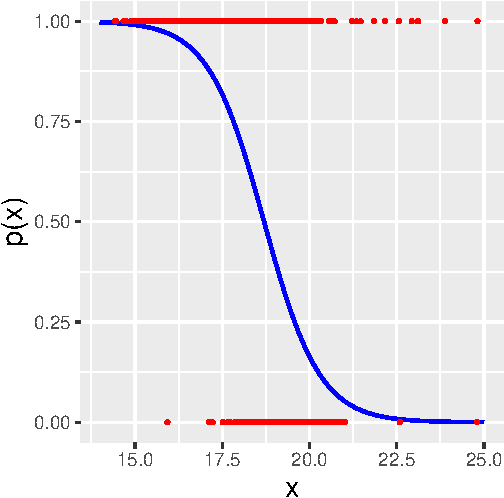
\includegraphics[keepaspectratio]{03-binomial_files/figure-latex/fig-logexp-1.pdf}}

}

\caption{\label{fig-logexp}An example of a logistic regression model.
The blue line is a sigmoid function: it represents the probability that
we would sample a datum with value 1 (as opposed to 0) as a function of
\(x\). The red points are the observed data.}

\end{figure}%

How do we learn a logistic regression model? In simple linear
regression, we determine values for \(\hat{\beta}_0\) and
\(\hat{\beta}_1\) by formulae, derived by minimizing the sum of squared
errors (SSE). For logistic regression, such simple formulae do not
exist, and so we estimate \(\beta_0\) and \(\beta_1\) via numerical
optimization of the likelihood function \[
\mathcal{L}(\beta_0,\beta_1 \vert \mathbf{y}) = \prod_{i=1}^n p_{Y}(y_i \vert \beta_0,\beta_1) = \prod_{i=1}^n p^{y_i}(1-p)^{1-y_i} = p^{\sum_{i=1}^n y_i} (1-p)^{n-\sum_{i=1}^n y_i} \,.
\] Specifically, we would take the first partial derivatives of
\(\mathcal{L}(\beta_0,\beta_1 \vert \mathbf{y})\) with respect to
\(\beta_0\) and \(\beta_1\), respectively, set them both to zero (thus
allowing us to equate the derivative expressions), and determine the
values \(\hat{\beta}_0\) and \(\hat{\beta}_1\) that jointly satisfy the
equated derivatives. These are the values at which the bivariate
likelihood surface achieves its maximum value. Note that because
numerical optimization is an iterative process, logistic regression
models are learned more slowly than simple linear regression models,
although one does not notice that slowness in typical analysis
situations.

Let's step back for a moment. Why would we want to learn a logistic
regression model in the first place? After all, it is a relatively
inflexible model that might lack the ability to mimic the true behavior
of \(p(x)\). The reason is that because we specify the mathematical form
of the model, we can after the fact examine the estimated coefficients
and perform \emph{inference}: we can examine how the response is
affected by changes in the predictor variables' values. This can be
important in, e.g., scientific contexts, where explaining how a model
works can be as important, if not more important, than its ability to
generate accurate and precise predictions. (This is in constrast to
commonly used machine learning models, whose mathematical forms cannot
be specified \emph{a priori} and are thus less interpretable after they
are learned.)

In simple linear regression, if we increase \(x\) by one unit, we can
immediately infer how the response value changes: \[
\hat{Y}' = \hat{\beta}_0 + \hat{\beta}_1 (x + 1) = \hat{\beta}_0 + \hat{\beta}_1 x + \hat{\beta}_1 = \hat{Y} + \hat{\beta}_1 \,.
\] For logistic regression, the situation is not as straightforward,
because \(p\) changes non-linearly as a function of \(x\). So we fall
back on the concept of the \emph{odds}, \[
O(x) = \frac{p(x)}{1-p(x)} = \exp\left(\hat{\beta}_0+\hat{\beta}_1x\right) \,,
\] or, often, its counterpart, the \emph{log-odds}: \[
\log O(x) = \hat{\beta}_0+\hat{\beta}_1x \,.
\] If, e.g., \(O(x) = 4\), then that means that, given \(x\), we are
four times more likely to sample a value of 1 than a value of 0. How
does the odds change if we add one unit to \(x\)? \begin{align*}
O(x+1) &= \exp\left(\hat{\beta}_0+\hat{\beta}_1(x+1)\right)\\
&= \exp\left(\hat{\beta}_0 + \hat{\beta}_1x\right)  \times \exp\left(\hat{\beta}_1\right) = O(x) \exp\left(\hat{\beta}_1\right) \,.
\end{align*} The odds change by a factor of
\(\exp\left(\hat{\beta}_1\right)\), which can be greater than or less
than one, depending on the sign of \(\hat{\beta}_1\). In terms of the
log-odds, this change is given by \[
\log O(x+1) = \log \left[ O(x) \exp\left(\hat{\beta}_1\right) \right] = \log O(x) + \hat{\beta}_1 \,.
\]

It is important to note that when we perform logistic regression, we are
simply estimating \(p(x)\), which is the probability that we would
sample a datum with value 1, given \(x\). How we choose to map \(p(x)\)
to either 0 or 1, i.e., how we determine whether or not we are
predicting that a datum belongs to ``Class 0'' or ``Class 1,'' is not
actually part of the logistic regression framework.
\emph{Classification} is a broad topic within statistical learning whose
details are beyond the scope of this book. We direct the interested
reader to, e.g., James et al. (2021).

\subsection{Examples}\label{examples-35}

\subsubsection{Logistic Regression in R}\label{logistic-regression-in-r}

\begin{quote}
When observed with a telescope, a star is a point-like object, as
opposed to a galaxy, which has some angular extent. Telling stars and
galaxies apart visually is thus, in relative terms, easy. However, if
the galaxy has an inordinately bright core because the supermassive
black hole at its center is ingesting matter at a high rate, that core
can outshine the rest of the galaxy so much that the galaxy appears to
be point-like. Such galaxies with bright cores are dubbed ``quasars,''
or ``quasi-stellar objects,'' and they are much harder to tell apart
from stars.
\end{quote}

\begin{quote}
Let's say we are given a dataset showing the difference in magnitude (a
logarithmic measure of brightness) at two wavelengths, for 500 stars and
500 quasars. The response variable is a factor variable with two levels,
which we will call ``Class 0'' (here, \texttt{QSO}) and ``Class 1''
(\texttt{STAR}). (The mapping of qualitative factors to quantitative
levels is by default alphabetical; as \texttt{STAR} comes after
\texttt{QSO}, \texttt{STAR} gets mapped to Class 1. One can always
override this default behavior.)
\end{quote}

\begin{quote}
We learn a simple logistic regression model using the \texttt{R}
function \texttt{glm()}, rather than \texttt{lm()}, and we specify
\texttt{family\ =\ binomial}, which means ``do logistic regression.''
(We can add additional arguments to, e.g., change the link function.)
\end{quote}

\begin{Shaded}
\begin{Highlighting}[]
\NormalTok{glm.out }\OtherTok{\textless{}{-}} \FunctionTok{glm}\NormalTok{(class }\SpecialCharTok{\textasciitilde{}}\NormalTok{ r, }\AttributeTok{data =}\NormalTok{ df, }\AttributeTok{family =}\NormalTok{ binomial)}
\FunctionTok{print}\NormalTok{(}\StringTok{"Deviance Residuals"}\NormalTok{)}
\end{Highlighting}
\end{Shaded}

\begin{verbatim}
[1] "Deviance Residuals"
\end{verbatim}

\begin{Shaded}
\begin{Highlighting}[]
\FunctionTok{summary}\NormalTok{(}\FunctionTok{residuals}\NormalTok{(glm.out))}
\end{Highlighting}
\end{Shaded}

\begin{verbatim}
     Min.   1st Qu.    Median      Mean   3rd Qu.      Max. 
-2.646515 -0.894956  0.033093  0.007907  0.843635  3.916292 
\end{verbatim}

\begin{Shaded}
\begin{Highlighting}[]
\FunctionTok{summary}\NormalTok{(glm.out)}
\end{Highlighting}
\end{Shaded}

\begin{verbatim}

Call:
glm(formula = class ~ r, family = binomial, data = df)

Coefficients:
            Estimate Std. Error z value Pr(>|z|)    
(Intercept) 23.44801    1.65428   14.17   <2e-16 ***
r           -1.25386    0.08817  -14.22   <2e-16 ***
---
Signif. codes:  0 '***' 0.001 '**' 0.01 '*' 0.05 '.' 0.1 ' ' 1

(Dispersion parameter for binomial family taken to be 1)

    Null deviance: 1386.3  on 999  degrees of freedom
Residual deviance: 1040.9  on 998  degrees of freedom
AIC: 1044.9

Number of Fisher Scoring iterations: 5
\end{verbatim}

\begin{quote}
The \texttt{summary()} of a learned logistic regression model is similar
to that for a linear regression model.
\end{quote}

\begin{quote}
A ``deviance residual'' is defined as \[
d_i = \mbox{sign}(p_i - \hat{p}_i) \sqrt{-2[p_i \log \hat{p}_i + (1-p_i)\log(1-\hat{p}_i)]} \,,
\] where \[
\hat{p}_i = \frac{\exp(\hat{\beta}_0+\hat{\beta}_1 x_i)}{1 + \exp(\hat{\beta}_0+\hat{\beta}_1 x_i)} \,.
\] The sum of the squared deviance residuals is equal to
\(-2 \log \mathcal{L}_{\mathrm{max}}\), where
\(\mathcal{L}_{\mathrm{max}}\) is the maximum value of the joint
likelihood of \(\hat{\beta}_0\) and \(\hat{\beta}_1\), given
\(\mathbf{x}\). Here, we observe that the deviance residuals are
seemingly well-balanced around zero.
\end{quote}

\begin{quote}
The coefficients can be translated to \(y\)-coordinate values as
follows: the intercept is \(e^{23.448}/(1+e^{23.448}) \rightarrow 1\)
(this is the probability that an object whose value of \texttt{r} is
equal to zero is a \texttt{STAR}), while the odds ratio is
\(O_{new}/O_{old} = e^{-1.254}\) (so that every time \texttt{r}
increases by one unit, the probability that a sampled datum is a star is
0.285 times what it had been before: the higher the value of \texttt{r},
the less and less likely that a sampled datum is actually a star, and
the more and more likely that it is a quasar\ldots at least, according
to the logistic regression model.
\end{quote}

\begin{quote}
The numbers in the other three columns of the coefficients section are
estimated numerically using the behavior of the likelihood function
(specifically, the rates at which it curves downward away from the
maximum). Some details about how the numbers are calculated are given in
an example in Section~\ref{sec-chap6covariance}. It suffices to say here
that if we assume that \(\hat{\beta}_0\) and \(\hat{\beta}_1\) are both
normally distributed random variables, we reject the null hypothesis
that the intercept is 0 (or equivalently that \(p = 1/2\) for all
\(x\)), and that \(\beta_1 = 0\).
\end{quote}

\begin{quote}
The null deviance is \(-2 \log \mathcal{L}_{max,o}\), where
\(\mathcal{L}_{max,o}\) is the maximum likelihood when \(\beta_1\) is
set to zero. The residual deviance is
\(-2 \log \mathcal{L}_{\mathrm{max}}\). The difference between these
values (here, 1386.3-1040.9 = 345.4), under the null hypothesis that
\(\beta_1 = 0\), is assumed to be sampled from a chi-square distribution
for 999-998 = 1 degree of freedom. (This is the large-sample
approximation that lies at the heart of Wilks' theorem, which we will
officially introduce in the context of the likelihood ratio test in
Section~\ref{sec-chap4hypothesis}.) The \(p\)-value is thus
\texttt{1\ -\ pchisq(345.4,\ 1)} or effectively zero: we emphatically
reject the null hypothesis that \(\beta_1 = 0\). While this hypothesis
test clearly indicates that \(\beta_1\) is not equal to zero, how can we
know whether the model itself fits to the data well in an absolute
sense? This is a model's ``goodness of fit,'' a concept we introduced in
Section~\ref{sec-chap3gof}. There is no unique answer to this question
in the context of logistic regression. Here we will show two ways by
which to build intuition about the quality of fit without going into
underlying detail. The first is an \emph{empirical logit} plot; see
Figure~\ref{fig-emplogit}. This plot shows the estimated log-odds for
\emph{binned} data as a function of the predictor variable, with the
fitted model overlaid. Here, we see that the data largely follow the
fitted model, indicating that the model is a relatively good
representation of the data-generating process.
\end{quote}

\begin{figure}

\centering{

\pandocbounded{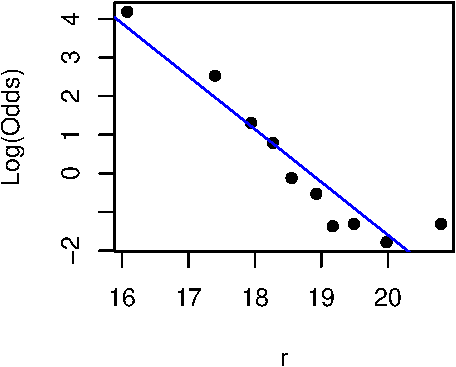
\includegraphics[keepaspectratio]{03-binomial_files/figure-latex/fig-emplogit-1.pdf}}

}

\caption{\label{fig-emplogit}An empirical logit plot in which we group
the data into ten bins. The fact that black points (representing the
binned data) largely follow the blue line (representing the predicted
response) indicates that the logistic regression model is a relatively
good representations of the data-generating process.}

\end{figure}%

\begin{quote}
A second way by which we can build intuition about the quality of fit of
the model is to utilize the Hosmer-Lemeshow test, in which the data are
binned (like they are in the construction of an empirical logit plot)
and a chi-square goodness-of-test test is carried out:
\end{quote}

\begin{Shaded}
\begin{Highlighting}[]
\FunctionTok{suppressMessages}\NormalTok{(}\FunctionTok{library}\NormalTok{(generalhoslem))}

\CommentTok{\# use of predict() does not give correct output in R 4.5.2}
\NormalTok{glm.predictions }\OtherTok{\textless{}{-}} \FunctionTok{predict.glm}\NormalTok{(glm.out, }\AttributeTok{type =} \StringTok{"response"}\NormalTok{)}
\CommentTok{\# note that "fitted(glm.out)" will give the same result}

\FunctionTok{logitgof}\NormalTok{(df}\SpecialCharTok{$}\NormalTok{class, glm.predictions) }\CommentTok{\# ten bins by default}
\end{Highlighting}
\end{Shaded}

\begin{verbatim}

    Hosmer and Lemeshow test (binary model)

data:  df$class, glm.predictions
X-squared = 50.774, df = 8, p-value = 2.901e-08
\end{verbatim}

\begin{quote}
Here we see that if we group the data into ten bins and run the
chi-square GoF test, the \(p\)-value is 2.9 \(\times\) 10\(^{-8}\): we
reject the null hypothesis that the logistic regression model is a good
representation of the data-generating process. (Although the empirical
logit plot indicates that it is not a \emph{bad} one. Observing an
ambiguous results like this is common in statistical practice!)
\end{quote}

\begin{quote}
The last metric we will discuss is the AIC, or Akaike Information
Criterion. The AIC is \(-2\) times the model likelihood (or here, the
deviance) plus two times the number of variables (here, 2, as the
intercept is counted as a variable). Adding the number of variables acts
to penalize those models with more variables: the improvement in the
maximum likelihood has to be sufficient to justify additional model
complexity. Discussion of the mathematical details of AIC is beyond the
scope of this book; it suffices to say that if we compute it when
learning a suite of different models, we would select the model with the
smallest value (while still keeping in mind that the ``best'' model may
not represent the data-generating process well in an absolute sense).
\end{quote}

\begin{quote}
We will wrap up by showing how one would start moving from estimating
the Class 1 probabilities for each datum towards predicting classes for
each datum. Logistic regression is not in and of itself a
``classifier'': it simply outputs probabilities. Naively, we would
classify an object with an estimated probability below 0.5 as being an
object of Class 0 and one with an estimated probability above 0.5 as
being an object of Class 1, but that only works in general if the
classes are balanced, i.e., if there are the same number of data of
Class 1 as of Class 0. (Here, ``works'' means ``acts to minimize
misclassification rates across both classes at the same time.'') If
there is class imbalance, then we will almost certainly have to change
0.5 to some other value for optimal classification. In the current
example, the classes \emph{are} balanced, and so putting the ``dividing
line'' at 0.5, as we do in Figure~\ref{fig-glmpred}, is an principled
choice.
\end{quote}

\begin{figure}

\centering{

\pandocbounded{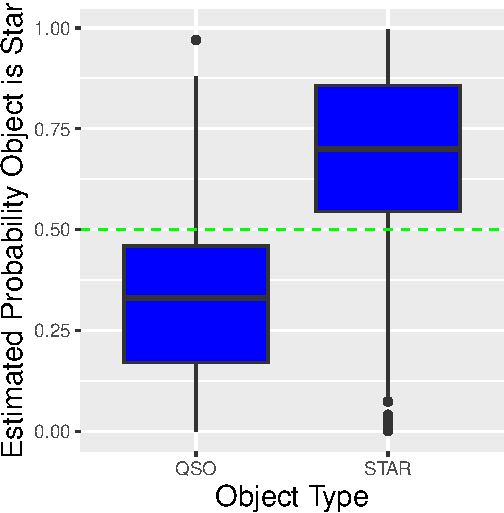
\includegraphics[keepaspectratio]{03-binomial_files/figure-latex/fig-glmpred-1.pdf}}

}

\caption{\label{fig-glmpred}Boxplots showing the estimated probability
that a datum is a star, as a function of the object type (quasar or
star). To convert estimated probabilities to predicted classes, one
would draw a dividing line between the two boxes: all objects with
probabilities below the line would be predicted to be quasars and all
others would be predicted to be stars. The line would be placed to,
e.g., minimize the number of misclassifications.}

\end{figure}%

\subsubsection{Beta Regression in R}\label{beta-regression-in-r}

\begin{quote}
The \texttt{R} package \texttt{betareg} includes a dataset called
\texttt{GasolineYield}, which records the ``{[}o{]}perational data of
the proportion of crude oil converted to gasoline after distillation and
fractionation.'' The key word here is ``proportion'': the response
variable \texttt{yield} has continuous values that are bounded to be
between 0 and 1. Here, we will regress \texttt{yield} upon one of the
possible predictor variables, \texttt{pressure}. (See
Figure~\ref{fig-betareg}. This figure indicates that we could have fit
to these data with a linear regression model with very little, if any,
change in the qualitative details of the results, but since we know that
the response variable is a proportion, beta regression is technically
the superior option.)
\end{quote}

\begin{Shaded}
\begin{Highlighting}[]
\FunctionTok{library}\NormalTok{(betareg)}
\end{Highlighting}
\end{Shaded}

\begin{verbatim}
Warning: package 'betareg' was built under R version 4.5.1
\end{verbatim}

\begin{Shaded}
\begin{Highlighting}[]
\FunctionTok{data}\NormalTok{(}\StringTok{"GasolineYield"}\NormalTok{, }\AttributeTok{package =} \StringTok{"betareg"}\NormalTok{)}
\NormalTok{betareg.out }\OtherTok{\textless{}{-}} \FunctionTok{betareg}\NormalTok{(yield }\SpecialCharTok{\textasciitilde{}}\NormalTok{ pressure, }\AttributeTok{data =}\NormalTok{ GasolineYield)}
\FunctionTok{summary}\NormalTok{(betareg.out)}
\end{Highlighting}
\end{Shaded}

\begin{verbatim}

Call:
betareg(formula = yield ~ pressure, data = GasolineYield)

Quantile residuals:
    Min      1Q  Median      3Q     Max 
-1.9374 -0.7088  0.2077  0.7557  1.6059 

Coefficients (mean model with logit link):
            Estimate Std. Error z value Pr(>|z|)    
(Intercept) -1.82595    0.22174  -8.234   <2e-16 ***
pressure     0.09480    0.04209   2.252   0.0243 *  

Phi coefficients (precision model with identity link):
      Estimate Std. Error z value Pr(>|z|)    
(phi)   14.616      3.607   4.051 5.09e-05 ***
---
Signif. codes:  0 '***' 0.001 '**' 0.01 '*' 0.05 '.' 0.1 ' ' 1 

Type of estimator: ML (maximum likelihood)
Log-likelihood: 30.71 on 3 Df
Pseudo R-squared: 0.1303
Number of iterations: 15 (BFGS) + 2 (Fisher scoring) 
\end{verbatim}

\begin{quote}
Note that by default, the link function is the logit function, meaning
that the only difference between this implementation of regression and
logistic regression is the assumption of the distribution of the
response (beta instead of Bernoulli, continuously valued instead of
discretely valued). See Figure~\ref{fig-betareg}. We see that the
summary output is qualitatively similar to what we observe for logistic
regression, with the exception of a new field dubbed ``Phi
coefficients.'' In the parameterization of the beta distribution used in
the \texttt{betareg} package, the variance of the response variable is
\(\mu(1-\mu)/(1+\phi)\), with \(\phi\) being a ``precision parameter'':
the lower the value of \(\phi\), the more dispersed the data are around
the regression line. All this being said, the only conclusion we can
make about \(\phi\) given the output is that, according to the
\(p\)-value, we can safely reject the null hypothesis that its value is
zero. For more information about beta regression, we refer the
interested reader to the \texttt{betareg} documentation.
\end{quote}

\begin{figure}

\centering{

\pandocbounded{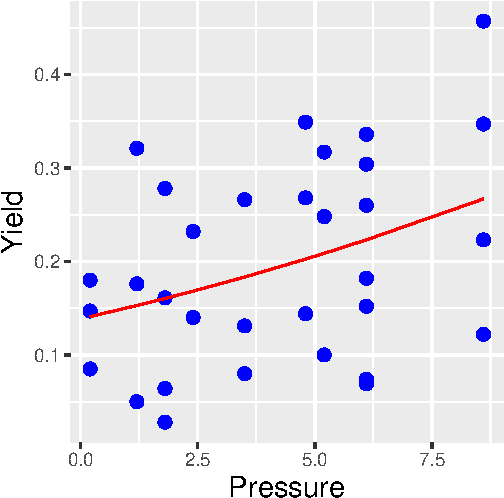
\includegraphics[keepaspectratio]{03-binomial_files/figure-latex/fig-betareg-1.pdf}}

}

\caption{\label{fig-betareg}A beta regression model (\(n = 32\)) in
which we regress \texttt{yield} upon \texttt{pressure}, given the
\texttt{GasolineYield} dataset of the \texttt{betareg} package. The
\(p\)-value associated with the \texttt{pressure} coefficient is 0.024;
we reject the null hypothesis that \texttt{yield} is not associated with
\texttt{pressure}. The coefficient is positive: as \texttt{pressure}
increases, the predicted \texttt{yield} also increases.}

\end{figure}%

\section{Naive Bayes Regression}\label{sec-chap3naivebayes}

What to take away from this section:

\begin{itemize}
\item
  Given a set of data tuples
  \(\{(x_{1,1},\ldots,x_{1,m},Y_1),\ldots,(x_{n,1},\ldots,x_{n,m},Y_n)\}\),
  where the \(x_{i,j}\)'s are either continuously or discretely valued,
  and where the \(Y_i\)'s can take on \(K\) discretely values, we can
  attempt to determine an association between \(\mathbf{x}\) and
  \(\mathbf{Y}\) by learning a \emph{Naive Bayes regression} model.
\item
  The Naive Bayes model combines Bayes' rule with an assumption that the
  data \(x_{\cdot,i}\) and \(x_{\cdot,j}\) are independently generated
  for all \(i \neq j\) to generate, for a given datum, predicted
  probabilities that it is associated with each of the \(K\) classes.
\item
  If we compare a suite of models, it will be the case that the Naive
  Bayes model will rarely, if ever, produce the best
  predictions\ldots but it is \emph{fast}, which makes it appropriate
  for time-sensitive tasks (like determining whether or not an email is
  spam).
\end{itemize}

The \emph{Naive Bayes} model is the basis for perhaps the simplest
probabilitic classifier, one that is used to, e.g., detect spam emails.
The meanings of the words ``Naive'' and ``Bayes'' will become more clear
below. Note that one would often see this model referred to as the
``Naive Bayes classifier.'' However, as noted in the last section, there
are actually two steps in classification, the first being the estimation
of probabilities that a given datum belongs to each class, and the
second being the mapping of those probabilities to class predictions. In
the previous section and here, we are only focusing on the generation of
predicted probabilities\ldots hence the title of this section.

(One might argue that the Naive Bayes model is a machine-learning model.
We would argue that it actually is not: the final form of a
machine-learning model is unknown before we start the modeling process
{[}e.g., the number of branches that will appear in a classification
tree model is unknown and is learned by the machine{]}, whereas with
Naive Bayes the mathematical form of the model is fully specified
\emph{a priori} and all we have to do is estimate the unknown
probabilities, which are the ``coefficients'' of the Naive Bayes model.)

Let's assume that we are in a similar setting as the one for logistic
regression, but instead of having a response that is a two-level factor
variable (i.e., one the represents two classes), the number of levels is
\(K \geq 2\). (So instead of just, e.g., ``chocolate'' and ``vanilla''
as our response variable values, we can add ``strawberry'' and other ice
cream flavors too!) The ultimate goal of the model is to assign
conditional probabilities for each response class, given a datum
\(\mathbf{x}\): \(p(C_k \vert \mathbf{x})\), where \(C_k\) denotes
``class \(k\).'' How do we derive this quantity?

The first step is to apply Bayes' rule (hence the ``Bayes'' in ``Naive
Bayes''): \[
p(C_k \vert \mathbf{x}) = \frac{p(C_k) p(\mathbf{x} \vert C_k)}{p(\mathbf{x})} \,.
\] The next step is to expand \(p(\mathbf{x} \vert C_k)\):
\begin{align*}
p(\mathbf{x} \vert C_k) &= p(x_1 \cup \ldots \cup x_p \vert C_k)\\
&= p(x_1 \vert x_2 \cup \ldots \cup x_p \cup C_k) p(x_2 \vert x_3 \cup \ldots \cup x_p \cup C_k) \cdots p(x_p \vert C_k) \,.
\end{align*} (This is the multiplicative law of probability in action,
as applied to a conditional probability. See Section 1.4.) The
expressions above are difficult to evaluate in practice, given all the
conditions that must be jointly applied. This is where the ``naive''
aspect of the model comes into play. We simplify the expression by
assuming (probably incorrectly!) that the predictor variables are all
mutually independent, so that \begin{align*}
&p(x_1 \vert x_2 \cup \ldots \cup x_p \cup C_k) p(x_2 \vert x_3 \cup \ldots \cup x_p \cup C_k) \cdots p(x_p \vert C_k)\\ \rightarrow ~~ &p(x_1 \vert C_k) \cdots p(x_p \vert C_k) 
\end{align*} and thus \[
p(C_k \vert \mathbf{x}) = \frac{p(C_k) \prod_{i=1}^p p(x_i \vert C_k)}{p(\mathbf{x})} \,.
\] OK\ldots where do we go from here?

We need to make further assumptions!

\begin{itemize}
\tightlist
\item
  We need to assign ``prior probabilities'' \(p(C_k)\) to each class.
  Common choices are \(1/K\) (we view each class as equally probable
  before we gather data) and \(n_k/n\) (the number of observed data of
  class \(k\) divided by the overall sample size).
\item
  We also need to assume probability mass and density functions
  \(p(x_j \vert C_k)\) for the \(j^{\mathrm{th}}\) predictor variable (a
  pmf if \(x_j\) is discrete and a pdf if \(x_j\) is continuous). It is
  convention to use binomial or multinomial pmfs, depending on the
  number of levels, with the observed proportions in each level
  informing the category probability estimate, and normal pdfs, with
  \(\hat{\mu}_j = \bar{x}_j\) and \(\hat{\sigma^2}_j = s_j^2\) (the
  sample variance).
\end{itemize}

Ultimately, this model depends on a number of (probably unjustified!)
assumptions. Why would we ever use it? Because the assumption of mutual
independence makes model evaluation \emph{fast}. Naive Bayes is rarely
the model underlying the best classifier for any given problem, but when
speed is needed (such as in the identification of spam email), one's
choices are limited. (As as general rule: if a model is simple to
implement, one should implement it, even if the \emph{a priori}
expectation is that another model will ultimately generate better
results. Because one never knows\ldots)

\subsection{Examples}\label{examples-36}

\subsubsection{Naive Bayes Regression With Categorical
Predictors}\label{naive-bayes-regression-with-categorical-predictors}

\begin{quote}
Let's assume that we have collected the following data:
\end{quote}

{\def\LTcaptype{none} % do not increment counter
\begin{longtable}[]{@{}ccc@{}}
\toprule\noalign{}
\endhead
\bottomrule\noalign{}
\endlastfoot
\(x_1\) & \(x_2\) & \(Y\) \\
Yes & Chocolate & True \\
Yes & Chocolate & False \\
No & Vanilla & True \\
No & Chocolate & True \\
Yes & Vanilla & False \\
No & Chocolate & False \\
No & Vanilla & False \\
\end{longtable}
}

\begin{quote}
We learn a Naive Bayes model given these data, in which we assume
``False'' is Class 0 and ``True'' is Class 1. If we have a new datum
\(\mathbf{x}\) = (``Yes'',``Chocolate''), what is the probability that
the response is ``True''?
\end{quote}

\begin{quote}
We seek the quantity \[
p(C_1 \vert \mathbf{x}) = \frac{p(C_1) p(\mathbf{x} \vert C_1)}{p(\mathbf{x})} = \frac{p(C_1) p(x_1 \vert C_1) p(x_2 \vert C_1)}{p(x_1 \cup x_2)} \,.
\] When we examine the data, we see that \(p(C_1) = 3/7\), as there are
three data out of seven with the value \(Y\) = ``True.'' Now, given
\(C_1\), at what rate do we observe ``Yes''? (One time out of
three\ldots so \(p(x_1 \vert C_1) = 1/3\).) What about ``Chocolate''?
(Two times out of three\ldots so \(p(x_2 \vert C_1) = 2/3\).) The
numerator is thus \(3/7 \times 1/3 \times 2/3 = 2/21\). The value of the
denominator, \(p(x_1 \cup x_2)\), is determined utilizing the Law of
Total Probability: \begin{align*}
p(x_1 \cup x_2) &= p(x_1 \vert C_1) p(x_2 \vert C_1) p(C_1) + p(x_1 \vert C_2) p(x_2 \vert C_2) p(C_2) \\
&= 2/21 + 2/4 \times 2/4 \times 4/7 = 2/21 + 4/28 = 2/21 + 3/21 = 5/21 \,.
\end{align*} And so now we know that \[
p(\mbox{True} \vert \mbox{Yes,Chocolate}) = \frac{2/21}{5/21} = \frac{2}{5} \,.
\]
\end{quote}

\subsubsection{Naive Bayes Regression With Continuous
Predictors}\label{naive-bayes-regression-with-continuous-predictors}

\begin{quote}
Let's assume we have the following data regarding credit-card defaults,
where \(x\) represents the credit-card balance and \(Y\) is a
categorical variable indicating whether a default has occurred:
\end{quote}

{\def\LTcaptype{none} % do not increment counter
\begin{longtable}[]{@{}
  >{\raggedright\arraybackslash}p{(\linewidth - 18\tabcolsep) * \real{0.0690}}
  >{\raggedright\arraybackslash}p{(\linewidth - 18\tabcolsep) * \real{0.1034}}
  >{\raggedright\arraybackslash}p{(\linewidth - 18\tabcolsep) * \real{0.1034}}
  >{\raggedright\arraybackslash}p{(\linewidth - 18\tabcolsep) * \real{0.1034}}
  >{\raggedright\arraybackslash}p{(\linewidth - 18\tabcolsep) * \real{0.1034}}
  >{\raggedright\arraybackslash}p{(\linewidth - 18\tabcolsep) * \real{0.1034}}
  >{\raggedright\arraybackslash}p{(\linewidth - 18\tabcolsep) * \real{0.1034}}
  >{\raggedright\arraybackslash}p{(\linewidth - 18\tabcolsep) * \real{0.1034}}
  >{\raggedright\arraybackslash}p{(\linewidth - 18\tabcolsep) * \real{0.1034}}
  >{\raggedright\arraybackslash}p{(\linewidth - 18\tabcolsep) * \real{0.1034}}@{}}
\toprule\noalign{}
\begin{minipage}[b]{\linewidth}\raggedright
\(x\)
\end{minipage} & \begin{minipage}[b]{\linewidth}\raggedright
1487.00
\end{minipage} & \begin{minipage}[b]{\linewidth}\raggedright
324.74
\end{minipage} & \begin{minipage}[b]{\linewidth}\raggedright
988.21
\end{minipage} & \begin{minipage}[b]{\linewidth}\raggedright
836.30
\end{minipage} & \begin{minipage}[b]{\linewidth}\raggedright
2205.80
\end{minipage} & \begin{minipage}[b]{\linewidth}\raggedright
927.89
\end{minipage} & \begin{minipage}[b]{\linewidth}\raggedright
712.28
\end{minipage} & \begin{minipage}[b]{\linewidth}\raggedright
706.16
\end{minipage} & \begin{minipage}[b]{\linewidth}\raggedright
1774.69
\end{minipage} \\
\midrule\noalign{}
\endhead
\bottomrule\noalign{}
\endlastfoot
\(Y\) & Yes & No & No & No & Yes & No & No & No & Yes \\
\end{longtable}
}

\begin{quote}
Let's now suppose someone came along with a credit balance of \$1,200.
According to the Naive Bayes model, given this balance, what is the
probability of a credit default?
\end{quote}

\begin{quote}
The Naive Bayes model in this particular case is \[
p(Y \vert x) = \frac{p(x \vert Y) p(Y)}{p(x \vert Y) p(Y) + p(x \vert N) p(N)} \,,
\] where we can observe immediately that \(p(Y) = 3/9 = 1/3\) and
\(p(N) = 6/9 = 2/3\). To compute, e.g., \(p(x \vert Y)\), we first
compute the sample mean and sample standard deviation for the observed
data for which \(Y\) is ``Yes'':
\end{quote}

\begin{Shaded}
\begin{Highlighting}[]
\NormalTok{x }\OtherTok{\textless{}{-}} \FunctionTok{c}\NormalTok{(}\FloatTok{1487.00}\NormalTok{, }\FloatTok{2205.80}\NormalTok{, }\FloatTok{1774.69}\NormalTok{)}
\FunctionTok{round}\NormalTok{(}\FunctionTok{mean}\NormalTok{(x), }\DecValTok{2}\NormalTok{)}
\end{Highlighting}
\end{Shaded}

\begin{verbatim}
[1] 1822.5
\end{verbatim}

\begin{Shaded}
\begin{Highlighting}[]
\FunctionTok{round}\NormalTok{(}\FunctionTok{sd}\NormalTok{(x), }\DecValTok{2}\NormalTok{)}
\end{Highlighting}
\end{Shaded}

\begin{verbatim}
[1] 361.78
\end{verbatim}

\begin{quote}
The mean is \$1,822.50 and the standard deviation is \$361.78, so the
probability density associated with observing \$1,200 is
\end{quote}

\begin{Shaded}
\begin{Highlighting}[]
\FunctionTok{dnorm}\NormalTok{(}\DecValTok{1200}\NormalTok{, }\AttributeTok{mean =} \FunctionTok{mean}\NormalTok{(x), }\AttributeTok{sd =} \FunctionTok{sd}\NormalTok{(x))}
\end{Highlighting}
\end{Shaded}

\begin{verbatim}
[1] 0.0002509367
\end{verbatim}

\begin{quote}
The density is 2.51 \(\times\) 10\(^{-4}\). As far as for those data for
which \(Y\) is ``No'':
\end{quote}

\begin{Shaded}
\begin{Highlighting}[]
\NormalTok{x }\OtherTok{\textless{}{-}} \FunctionTok{c}\NormalTok{(}\FloatTok{324.74}\NormalTok{, }\FloatTok{988.21}\NormalTok{, }\FloatTok{836.30}\NormalTok{, }\FloatTok{927.89}\NormalTok{, }\FloatTok{712.28}\NormalTok{, }\FloatTok{706.16}\NormalTok{)}
\FunctionTok{dnorm}\NormalTok{(}\DecValTok{1200}\NormalTok{, }\AttributeTok{mean =} \FunctionTok{mean}\NormalTok{(x), }\AttributeTok{sd =} \FunctionTok{sd}\NormalTok{(x))}
\end{Highlighting}
\end{Shaded}

\begin{verbatim}
[1] 0.0002748351
\end{verbatim}

\begin{quote}
The density is 2.75 \(\times\) 10\(^{-4}\). Thus \[
p(Y \vert x) = \frac{2.51 \cdot 0.333}{2.51 \cdot 0.333 + 2.75 \cdot 0.667} = \frac{0.834}{0.834 + 1.834} = 0.313 \,.
\] We would predict that there is roughly a 1 in 3 chance that a person
with a credit balance of \$1,200 will default on their debt.
\end{quote}

\subsubsection{Naive Bayes in R}\label{naive-bayes-in-r}

\begin{quote}
In the previous section, we applied logistic regression to the problem
of differentiating between stars and quasars. Here, we repeat the
exercise using a Naive Bayes model, as coded in \texttt{R}'s
\texttt{e1071} package.
\end{quote}

\begin{Shaded}
\begin{Highlighting}[]
\FunctionTok{library}\NormalTok{(e1071)}
\NormalTok{nb.out }\OtherTok{\textless{}{-}} \FunctionTok{naiveBayes}\NormalTok{(class }\SpecialCharTok{\textasciitilde{}}\NormalTok{ r, }\AttributeTok{data =}\NormalTok{ df)}
\NormalTok{nb.out}
\end{Highlighting}
\end{Shaded}

\begin{verbatim}

Naive Bayes Classifier for Discrete Predictors

Call:
naiveBayes.default(x = X, y = Y, laplace = laplace)

A-priori probabilities:
Y
 QSO STAR 
 0.5  0.5 

Conditional probabilities:
      r
Y          [,1]      [,2]
  QSO  19.35770 0.8282726
  STAR 17.96389 1.3651572
\end{verbatim}

\begin{quote}
The summary of the model shows that the classes are balanced (as the
\texttt{A-priori\ probabilities} are 0.5 for each class). It then shows
the estimated distributions of \texttt{r} values for quasars (a normal
with estimated mean 19.358 and standard deviation 0.828) and stars (mean
17.964 and standard deviation 1.365). See Figure~\ref{fig-nbplot}.
\end{quote}

\begin{figure}

\centering{

\pandocbounded{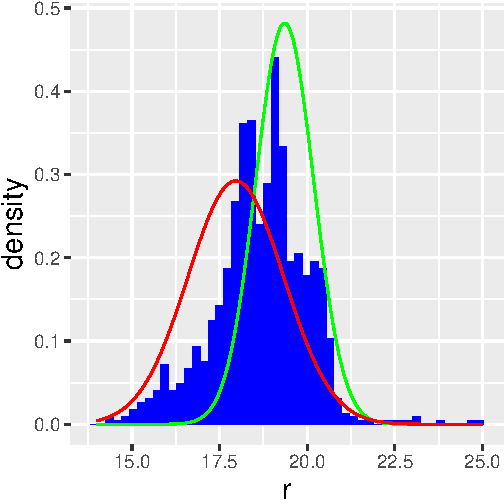
\includegraphics[keepaspectratio]{03-binomial_files/figure-latex/fig-nbplot-1.pdf}}

}

\caption{\label{fig-nbplot}An illustration of the Naive Bayes regression
model, as applied to the star-quasar dataset. The red curve is the
estimated normal probability density function for stars, while the green
curve is the estimated pdf for quasars. Because the two classes in this
example are balanced, we can state that where the amplitude of the red
curve is higher, the predicted class would be \texttt{STAR}; otherwise,
it would be \texttt{QUASAR}.}

\end{figure}%

\begin{quote}
To generate model predictions, we use a function call similar to that
utilized in logistic regression:
\end{quote}

\begin{Shaded}
\begin{Highlighting}[]
\NormalTok{nb.predictions }\OtherTok{\textless{}{-}} \FunctionTok{predict}\NormalTok{(nb.out, }\AttributeTok{newdata =}\NormalTok{ df, }\AttributeTok{type =} \StringTok{"raw"}\NormalTok{)[, }\DecValTok{2}\NormalTok{]}
\end{Highlighting}
\end{Shaded}

\begin{quote}
The \texttt{predict()} function outputs a matrix showing the
probabilities associated with each response class. Since here we are
interested in the probability of sampling a datum of value 1 (a ``Class
1'' datum), we extract the second column of the output matrix. In
Figure~\ref{fig-nbpred}, we show the predicted probabilities as a
function of the object type; the reader should compare this figure with
Figure~\ref{fig-glmpred}.
\end{quote}

\begin{figure}

\centering{

\pandocbounded{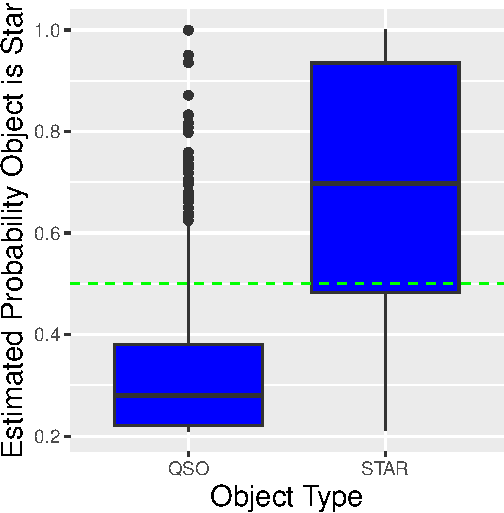
\includegraphics[keepaspectratio]{03-binomial_files/figure-latex/fig-nbpred-1.pdf}}

}

\caption{\label{fig-nbpred}Boxplots showing the estimated probability
that a datum is a star, as a function of the object type (quasar or
star). To convert estimated probabilities to predicted classes, one
would draw a dividing line between the two boxes: all objects with
probabilities below the line would be predicted to be quasars and all
others would be predicted to be stars. The line would be placed to,
e.g., minimize the number of misclassifications.}

\end{figure}%

\section{Exercises}\label{sec-chap3exercises}

\begin{enumerate}
\def\labelenumi{\arabic{enumi}.}
\item
  Let \(X_1,...,X_n\) be \(n\) data drawn from a \(\mathcal{N}(2,4)\)
  distribution. Write down the probability that exactly \(m\) of the
  \(n\) data have values \(> 2\).
\item
  You are a habitual buyer of raffle tickets. Each ticket costs \$1, and
  each time you buy a ticket, you have a 40\% chance of having a winning
  ticket, for which you will receive \$3. You decide to keep buying
  tickets until you win for the first time. Let the random variable
  \(F\) denote the total number of \emph{losing} tickets that you buy,
  and let \(W\) denote the total amount of money you win (or lose!). (a)
  \(F\) is sampled from what distribution that has what parameter
  value(s)? (b) What is the probability that you will end up making
  money, i.e., what is \(P(W > 0)\)? (c) Let's say instead of buying
  until you win, you decide you will buy exactly two tickets, then stop.
  What is the probability of buying a winning ticket exactly once, given
  that you buy at least one winning ticket?
\item
  Suppose 50\% of licensed drivers in a state are insured. If three
  licensed drivers are selected at random, what is the expected number
  of insured drivers given that the number of insured drivers is odd?
  (Assume the state's population is effectively infinite, so that the
  probability of selecting an insured driver stays constant from trial
  to trial.)
\item
  In an experiment, you take shots at a target until you hit that target
  twice. On any given shot, you have a 50\% change of hitting the
  target. (a) What is the probability that you hit the target for the
  second time on your fourth shot overall? (b) You run your experiment
  twice. What is the probability of needing to take two shots one of the
  experiments to hit the target twice, and three shots during the other
  one to hit the target twice? Assume the results are independent (and
  of course identically distributed). (c) Let's suppose you do not
  actually know the success probability \(p\), and you wish to determine
  a one-sided 90\% upper bound on \(p\). As you are dealing with a
  discrete distribution, you need to build a \texttt{uniroot()}-style
  interval estimator. In your code, what value would you adopt for
  \(q\)?
\item
  You collect \(n=4\) iid samples from the following distribution:
  \begin{eqnarray*}
  f_X(x) = \left\{ \begin{array}{cc} 3x^2 & 0 \leq x \leq 1 \\ 0 & \mbox{otherwise} \end{array} \right. \,.
  \end{eqnarray*} (a) Write down the sampling distribution for the
  minimum observed value, \(X_{(1)}\). (b) The sampling distribution for
  the maximum observed value is \(g_{(4)}(x) = 12x^{11}\). What is
  \(E[X_{(4)}]\)?
\item
  You are to sample \(n = 3\) data from the following distribution:
  \begin{eqnarray*}
  f_X(x) = \left\{ \begin{array}{cc} x & 0 \leq x \leq \sqrt{2} \\ 0 & \mbox{otherwise} \end{array} \right. \,.
  \end{eqnarray*} (a) Specify the distribution from which \(X_{(3)}\) is
  to be sampled. (b) Specify the variance of the distribution you
  derived in part (a).
\item
  If we sample 3 iid data from a Uniform(0,1) distribution, what is the
  probability that the median value lies between 1/3 and 2/3?
\item
  You sample three data from a Exp(1) distribution. What is the expected
  value for the median datum, i.e., the second ordered datum?
\item
  Let the cdf for a given distribution be \(F_X(x) = x^3\) for
  \(x \in [0,1]\), and let's assume that you have sampled \(n\) iid data
  from this distribution. (a) What is the pdf within the domain
  \(x \in [0,1]\)? (b) What is the pdf for \(X_{(n)}\) within the domain
  \(x \in [0,1]\)? (c) What is the cdf for \(X_{(n)}\) within the domain
  \(x \in [0,1]\)? (d) What is \(E[X_{(n)}]\)?
\item
  You sample \(n = 2\) iid random variables from a distribution with pdf
  \begin{eqnarray*}
  f_X(x) = \frac12 x \,,
  \end{eqnarray*} for \(x \in [0,2]\). (a) What is \(F_X(x)\) within the
  domain \([0,2]\)? (b) What is \(f_{(2)}(x)\)? (c) What is
  \(E[X_{(2)}]\)? (d) Are \(X_{(1)}\) and \(X_{(2)}\) independent random
  variables?
\item
  Find the asymptotic distribution of the MLE of \(n\) i.i.d. samples
  from the Bernoulli distribution with parameter \(p\).
  (\(p_X(x) = p^x(1-p)^{1-x}\) for \(x = \{0,1\}\) and for
  \(p \in (0,1)\).)
\item
  You are given \(n\) iid data that are sampled from the following pmf:
  \begin{equation*}
  p_X(x) = (1-p)^{x-1}p \,, 
  \end{equation*} with \(0 < p < 1\) and \(x = \{1,2,3,\ldots\}\). For
  this distribution, \(E[X] = 1/p\) and \(V[X] = (1-p)/p^2\). (a) What
  is the maximum likelihood estimator for \(1/p\)? Note: you are not
  required to confirm that the derivative of the score function is
  negative at \(1/p = \widehat{1/p}_{MLE}\). Also note: a property of
  MLEs may help you here. (b) Write down \(V[\widehat{1/p}_{MLE}]\),
  i.e., the variance of the MLE for \(1/p\).
\item
  The probability mass function for the logarithmic distribution is
  \begin{eqnarray*}
  p_X(x) = -\frac{1}{\log(1-p)} \frac{p^x}{x} \,,
  \end{eqnarray*} where \(x \in \{1,2,3,...\}\). You sample \(n\) iid
  data from this distribution. Write down a sufficient statistic for
  \(p\).
\item
  You are given the following probability density function:
  \begin{equation*}
  f_X(x) = a b x^{a-1} (1-x^a)^{b-1} \,,
  \end{equation*} defined over the domain \(0 < x < 1\). \(a\) and \(b\)
  are the parameters of the distribution, and both are positive and
  real-valued. Let \(\mathbf{X} = \{X_1,\cdots,X_n\}\) be \(n\)
  i.i.d.\textasciitilde samples from this distribution. (a) If you are
  able to define joint sufficient statistics for \(a\) and \(b\), write
  them down; otherwise, explain why you cannot. (b) Now, let \(a=1\).
  What is a sufficient statistic for \(b\)?
\item
  You sample \(n\) iid data from the following distribution:
  \begin{eqnarray*}
  f_X(x) = \frac{x}{\beta^2} e^{-x/\beta} \,,
  \end{eqnarray*} where \(x \geq 0\) and \(\beta > 0\), and where
  \(E[X] = 2\beta\) and \(V[X] = 2\beta^2\). (a) Write down a sufficient
  statistic for \(\beta\) that arises directly from likelihood
  factorization. (b) Using your answer from part (a), determine the MVUE
  for \(\beta\). (c) Compute the variance of the MVUE for \(\beta\). (d)
  Compute the Cramer-Rao Lower Bound for the MVUE for \(\beta\).
\item
  Let \(X_1,\ldots, X_n\) be \(n\) iid samples from the following
  distribution, where \(\theta > 0\), \begin{eqnarray*}
  f_X(x) = \frac{1}{\theta} \exp\left(x-\frac{1}{\theta} e^x\right) \,.
  \end{eqnarray*} Note that \(e^X \sim \text{Exp}(\theta)\) (=
  Gamma(1,\(\theta\))) and
  \(Y = \sum_{i=1}^n e^{X_i} \sim \text{Gamma}(n,\theta)\) (with
  \(E[Y] = n\theta\) and \(V[Y] = n\theta^2\)). (a) Find a sufficient
  statistic for \(\theta\) using the factorization criterion. (b) Find
  the MVUE for \(\theta\). (c) Find the MVUE for \(\theta^2\).
\item
  Let's assume that we have sampled \(n\) iid data,
  \(\{X_1,\ldots,X_n\}\), from a Maxwell-Boltzmann distribution with pdf
  \begin{eqnarray*}
  f_X(x) = \sqrt{\frac{2}{\pi}} \frac{x^2}{a^3} e^{-x^2/(2a^2)} \,,
  \end{eqnarray*} where \(x > 0\) and \(a > 0\). The expected value and
  variance for an MB-distributed random variable are \begin{eqnarray*}
  E[X] = 2 a \sqrt{\frac{2}{\pi}} ~~~ \mbox{and} ~~~ V[X] = a^2 \frac{(3 \pi - 8)}{\pi} 
  \end{eqnarray*} respectively. (a) Identify a sufficient statistic for
  \(a^2\). (b) Derive \(E[X^2]\). (Hint: there is no need for
  integration here.) (c) Determine the MVUE for \(a^2\). (d) Can we use
  an invariance principle to state that the MVUE for \(a\) is
  \((\widehat{a^2}_{MVUE})^{1/2}\)?
\item
  You sample a single datum \(X\) from the following pdf:
  \begin{eqnarray*}
  f_X(x) = \frac{\theta}{2^\theta} x^{\theta-1} \,,
  \end{eqnarray*} where \(x \in [0,2]\) and \(\theta > 0\). Construct
  the most powerful level-\(\alpha\) test of \(H_o: \theta = \theta_o\)
  versus \(H_a: \theta = \theta_a\), where \(\theta_a > \theta_o\). Is
  your hypothesis test a uniformly most powerful hypothesis test?
\item
  A common distribution used for the lengths of life of physical systems
  is the Weibull. Let \(\{X_1,\ldots,X_n\}\) be \(n\) iid data sampled
  from this distribution: \begin{eqnarray*}
  f_X(x) = \frac{\theta}{\beta} \hspace{1mm} x^{\theta-1} \hspace{1mm} \exp\left(-\frac{x^\theta}{\beta}\right) \hspace{5mm} x,\beta, \theta >0
  \end{eqnarray*} Assume that \(\theta\) is known and that \(\beta\) is
  freely varying, and that we are interested in finding the most
  powerful test of \(H_o: \beta = \beta_o\) versus
  \(H_a: \beta = \beta_a\), where \(\beta_a > \beta_o\), at the level
  \(\alpha\).
\end{enumerate}

\begin{enumerate}
\def\labelenumi{(\alph{enumi})}
\tightlist
\item
  What is a sufficient statistic for \(\beta\)? (Do not include a minus
  sign.)
\item
  Working with the Weibull directly is difficult; however, it turns out
  that \(X^\theta \sim \text{Exp}(\beta)\). What is the distribution of
  the sufficient statistic found in part (a), and what are the parameter
  values? (This will require examining the gamma distribution and its
  properties.)
\item
  Write, in \texttt{R} code, the rejection-region boundary for the test.
\end{enumerate}

\begin{enumerate}
\def\labelenumi{\arabic{enumi}.}
\setcounter{enumi}{19}
\tightlist
\item
  Let \(\{X_1,\ldots,X_n\}\) be \(n\) iid data sampled from the
  following distribution: \begin{eqnarray*}
  f_{X}(x) = \left\{ \begin {array}{ll} \frac{1}{\theta}\exp\left(-\frac{1}{\theta}(x-b)\right) & x > b, \theta > 0 \\ 0&\mbox{otherwise} \end{array} \right. \,.
  \end{eqnarray*}
\end{enumerate}

\begin{enumerate}
\def\labelenumi{(\alph{enumi})}
\tightlist
\item
  Derive the moment-generating function for \(X\).
\item
  Now derive the mgf for \(\sum_{i=1}^n X_i\).
\item
  The answer for (b) contains the term \(e^{nbt}\). Going back to our
  original discussion of the method of moment-generating functions, this
  means that we can write that
  \(\sum_{i=1}^n X_i = nb + \sum_{i=1}^n U_i\). What distribution is
  \(\sum_{i=1}^n U_i\) sampled from? (Hint: look at the the rest of the
  mgf for \(\sum_{i=1}^n X_i\) and, if necessary, refer back to the
  previous problem.)
\item
  Write, in \texttt{R} code, the rejection-region boundary for the
  \(\alpha\)-level test of \(H_o : \theta = \theta_o\) versus
  \(H_a : \theta < \theta_o\). Is this a uniformly most powerful test of
  these hypotheses?
\end{enumerate}

\begin{enumerate}
\def\labelenumi{\arabic{enumi}.}
\setcounter{enumi}{20}
\item
  In an experiment, you sample \(n\) data from the distribution:
  \begin{eqnarray*}
  f_X(x) = \theta e^{-\theta x} \,,
  \end{eqnarray*} where \(x \geq 0\), \(\theta > 0\), and
  \(E[X] = 1/\theta\). You wish to test the null hypothesis
  \(H_o : \theta_o = 4\) versus \(H_a : \theta_a = 2\). (a) Define the
  most powerful hypothesis test. By ``define,'' we mean write down a
  rejection region of the form \(Y < y_{\mathrm{RR}}\) or
  \(Y > y_{\mathrm{RR}}\), where you plug in a specific statistic for
  \(Y\). (You cannot evaluate \(y_{\mathrm{RR}}\) given the information
  you have here\ldots that can stay as is.) (b) The cdf of the sampling
  distribution for the appropriate statistic in part (a) is
  \(\gamma(n,\theta y)/(n-1)!\), where \(\gamma(\cdot,\cdot)\) is the
  lower incomplete gamma function. Given this information, and given
  what you would have to do to define the rejection region boundary, can
  you conclude that we are defining a uniformly most powerful test?
\item
  Let's assume that we have sampled \(n\) iid data from a Binom(\(k,p\))
  distribution, and that we wish to test \(H_o: p = p_o\) versus
  \(H_a: p > p_o\). For our statistic, we will use
  \(Y = \sum_{i=1}^n X_i\). (a) What is the sampling distribution for
  \(Y\)? Provide the name and the value(s) of the parameters. (b) You
  code elements of the test in \texttt{R}. Assume you have the
  initialized variables \texttt{alpha}, \texttt{n}, \texttt{k},
  \texttt{y.obs}, \texttt{p.o}, and \texttt{p.a} at your disposal. Write
  out the (one-line!) function call you'd use to compute the rejection
  region boundary. (c) Now provide code of the \(p\)-value. Include a
  discreteness correction factor if it is needed.
\item
  The negative inverse link function is \(-(Y \vert x)^{-1}\). Assume
  that we are in a simple setting (i.e., that there is one predictor
  variable), and write the regression line formula \(Y \vert x\) as a
  function of \(\beta_0\), \(\beta_1\), and \(x\).
\item
  You use \texttt{R} to learn a logistic regression model, and you
  observe the output shown below: (a) What is the sample size \(n\)?
  (Hint: take into account how many parameter values are being estimated
  to convert a number shown in the output to the sample size.) (b) What
  is the value of \(-2\log\mathcal{L}_{\mathrm{max}}\) for the model in
  which \(\beta_1\) is set to zero? (c) What is the value of \(O(x)\)
  for \(x = 0\)? You may leave your answer in the form \(e^a\) or
  \(\log(a)\) or \(\sqrt{a}\), etc., while being sure to fill in the
  value of the constant \(a\). (d) Do the odds \emph{increase} as \(x\)
  increases, or do the odds \emph{decrease} as \(x\) increases?
\end{enumerate}

\begin{center}
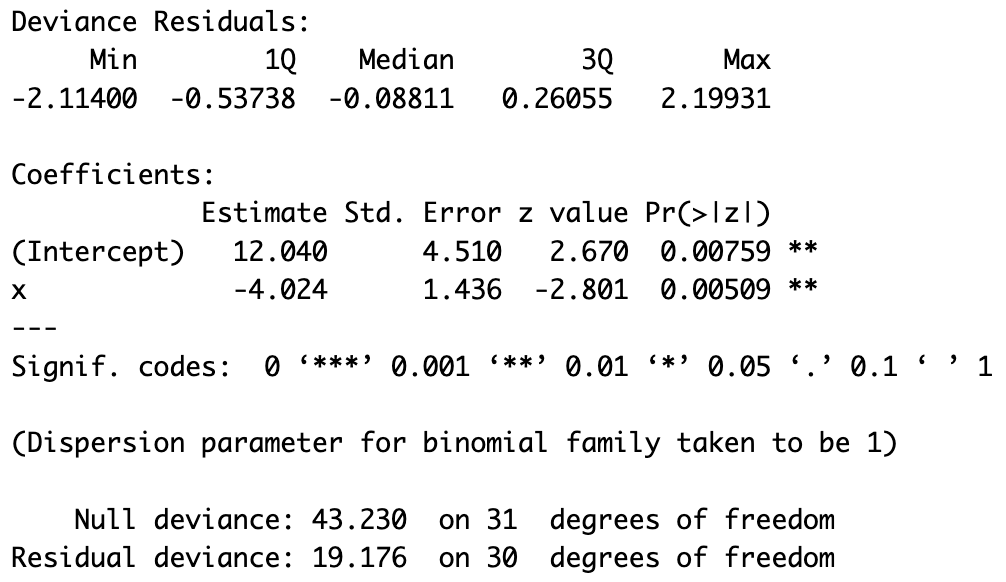
\includegraphics[width=0.75\linewidth,height=\textheight,keepaspectratio]{figures/logreg.png}
\end{center}

\begin{enumerate}
\def\labelenumi{\arabic{enumi}.}
\setcounter{enumi}{24}
\tightlist
\item
  Below is the observed output from \texttt{R}'s \texttt{glm()} function
  when learning a logistic regression model. For these data, Class 0 is
  \texttt{No} (not a student) and Class 1 is \texttt{Yes} (is a
  student). (a) If the balance is \$589, then the predicted probability
  that the datum belongs to the \texttt{Yes} class is 0.1. What is the
  odds ratio for \$589 dollars? (b) What is the odds ratio if the
  balance is \$689? (c) For the first datum, the observed response is
  \texttt{No} and the predicted probability that the datum is of the
  \texttt{Yes} class is 0.07. Compute the deviance for this datum. (d)
  Whoops\ldots the null deviance value got expunged from the output.
  Would this value be higher or lower than the observed residual
  deviance value?
\end{enumerate}

\begin{verbatim}
Deviance Residuals:
    Min       1Q   Median       3Q      Max
-1.1243  -0.5539  -0.4409  -0.3460   2.4901

Coefficients:
              Estimate Std. Error z value Pr(>|z|)
(Intercept) -3.0616324  0.3936314  -7.778 7.37e-15 ***
Balance      0.0014684  0.0004124   3.561  0.00037 ***
---
Signif. codes:  0 ‘***’ 0.001 ‘**’ 0.01 ‘*’ 0.05 ‘.’ 0.1 ‘ ’ 1

Residual deviance: 221.47  on 308  degrees of freedom 
AIC: 225.47 
\end{verbatim}

\begin{enumerate}
\def\labelenumi{\arabic{enumi}.}
\setcounter{enumi}{25}
\tightlist
\item
  Refer to the displayed data below. Here, \texttt{x1} and \texttt{x2}
  are the two predictor variables, and \(Y\) is the response variable.
  Use these data to learn a Naive Bayes model and use that model to
  compute
  \(p(0 \vert \mbox{Yes},\mbox{False}) = p(0 \vert \mbox{Y},\mbox{F})\).
  Leave your answer as a fraction. Assume that \(p(C_k) = n_k/n\), and
  that you would estimate \(p(x \vert C_k)\) as the proportion of times
  you observe a particular datum value \(x\) (e.g., True) given \(C_k\).
\end{enumerate}

\begin{center}
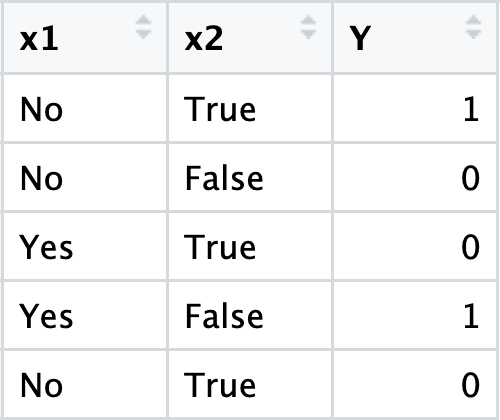
\includegraphics[width=0.4\linewidth,height=\textheight,keepaspectratio]{figures/nb.png}
\end{center}

\begin{enumerate}
\def\labelenumi{\arabic{enumi}.}
\setcounter{enumi}{26}
\item
  You are given the following pdf: \begin{eqnarray*}
  f_X(x) = \left\{ \begin{array}{cc} 2(1-x) & 0 \leq x \leq 1 \\ 0 & \mbox{otherwise} \end{array} \right. \,. 
  \end{eqnarray*} An associated cost is \(C = 10X\). (a) Identify the
  ``named'' distribution for \(X\) and state its parameters. (b) Given
  your answer for (a), determine \(E[X]\) and \(E[X^2]\). (c) Now
  determine \(E[C]\) and \(V[C]\).
\item
  You are given the following cdf: \begin{eqnarray*}
  F_X(x) = \left\{ \begin{array}{cc} 0 & x < 0 \\ 6x^2 - 8x^3 + 3x^4 & 0 \leq x \leq 1 \\ 1 & x > 1 \end{array} \right. \,.
  \end{eqnarray*} (a) \(F_X(x)\) is the cdf for what ``named''
  distribution? (b) What is the expected value of \(X\)?
\item
  You are given \(X \sim\) Beta(2,3). What is \(E[X^2]\)?
\item
  You sample 3 data from a Beta(3,1) distribution. (a) Write down the
  pdf for the median of the sampled data. (b) Compute the expected value
  for the median of the sampled data.
\item
  You are given the following distribution: \begin{eqnarray*}
  f_X(x) = c x (1-x) \,,
  \end{eqnarray*} where \(x \in [0,1]\) and \(c\) is a constant. (a)
  Identify this distribution by name and provide the value(s) of its
  parameter(s). (b) Determine the numerical value of the constant \(c\).
  (c) Is the distribution symmetric about its mean value or it is a
  skewed distribution? (d) Compute \(P(X \leq 1/4 \vert X \leq 1/2)\).
  Leave your answer as a fraction.
\item
  Twenty-one (21) students enter a hallway off of which are three rooms.
  A researcher expects each student to randomly choose a room to enter
  (and to stay in!). That researcher observes that 10 students choose
  Room A, 5 students choose Room B, and 6 students choose Room C, and
  she decides to use these data to perform a test of the null hypothesis
  \(p_1 = p_2 = p_3\) at the level \(\alpha = 0.1\). (a) Choose an
  appropriate hypothesis test and evaluate the test statistic. To be
  clear, your final answer should be a number. (b) What is the number of
  degrees of freedom associated with the test statistic? (c) The
  rejection region boundary value is 4.61. Do we reject the null
  hypothesis?
\item
  A political scientist has developed four pamphlets with different
  types of information about climate change -- one focused on
  environmental impact, one on economic impact, one on socio-cultural
  impact, and one about the origins of climate change. She prints 100 of
  each and randomly gives them out, asks people to read them, and
  records their answer to the question: how much money should the
  government spend on counteracting climate change? The answer options
  are: {[}a{]} more than, {[}b{]} as much as, and {[}c{]} less than they
  currently do. She plans to do a chi-square test to check whether
  willingness to spend government funding is related to which pamphlet
  the respondent read. (Note that she does not segment the respondents
  into groups.) (a) What kind of chi-square test is conducted here
  (goodness-of-fit, independence, or homogeneity)? (b) The observed test
  statistic turns out to be \(w_{\mathrm{obs}} = 24.3\). How many terms
  did the researcher have to sum over to compute this statistic? (c) The
  test statistic follows a chi-square distribution with \(m\) degrees of
  freedom. What is the value of \(m\)? (d) Which of the following
  expressions corresponds to the \(p\)-value associated with the test
  carried out in part (a): (i) \(P(W \geq w_{\mathrm{obs}})\), (ii)
  \(P(W \leq w_{\mathrm{obs}})\), (iii)
  \(P(\frac{(n-1) W }{ \sigma^2} \geq w_{\mathrm{obs}})\), or (iv)
  \(P(\frac{(n-1) W}{\sigma^2} \leq w_{\mathrm{obs}})\)? (\(W\) is the
  random variable, chi-square-distributed for \(m\) degrees of freedom;
  \(n\) is the sample size; and \(\sigma^2\) is the population
  variance.)
\item
  You are recording the amount of time that elapses between when one
  person walks through a particular door until the next person walks
  through that same door. You have a weird stopwatch that changes from 0
  to 1 after one minute, and from 1 to 2 after two minutes. That's it.
  You take 100 measurements, and your data are given below. You wish to
  test the null hypothesis that each elapsed time is sampled from an
  exponential distribution with mean \(\beta\) = 1 minute. (a) Under
  this null hypothesis, the probability that someone ends up in the
  category ``1-2 minutes'' is \(\int_1^2 e^{-x} dx\). Explain why this
  is and calculate the probability. (b) Carry out an appropriate test to
  test the null hypothesis, provide either the rejection region or the
  \(p\)-value, and state your conclusion. Assume \(\alpha = 0.05\). (c)
  A friend of yours decides they will repeat the experiment you've done,
  including the statistical analysis, but he is in a hurry and decides
  that he will only take 10 measurements overall. Explain to your friend
  why his experimental ``design'' is flawed.
\end{enumerate}

{\def\LTcaptype{none} % do not increment counter
\begin{longtable}[]{@{}ccc@{}}
\toprule\noalign{}
\endhead
\bottomrule\noalign{}
\endlastfoot
0-1 min & 1-2 min & \textgreater2 min \\
52 & 23 & 25 \\
\end{longtable}
}

\begin{enumerate}
\def\labelenumi{\arabic{enumi}.}
\setcounter{enumi}{34}
\item
  You play a (long) game in which you shoot 180 shots at a 3-by-3 square
  target, inside of which is a 1-by-1 square bullseye. Of your shots, 30
  hit the bullseye while the remainder all hit the target, but hit
  outside the bullseye. You wish to test the null hypothesis that your
  shots hit the target at random locations. (a) Specify the number of
  shots that are expected to hit outside of, and inside of, the bullseye
  if the null hypothesis is correct. (b) Compute the value of an
  appropriate statistic for this test. (c) Specify the sampling
  distribution for this statistic (if the null hypothesis is correct);
  give the name and the values of any distribution parameters. (d) The
  rejection region boundary for this test is 3.841. State a conclusion
  regarding the null hypothesis: ``reject'' or ``fail to reject.''
\item
  We collect \(k\) independent datasets, and perform hypothesis tests
  for the population mean given each. When we are done, we have \(k\)
  separate \(p\)-values, which are all independent of each other. In
  every case, it turns out that the the null hypothesis is correct. Let
  \(X\) represent the number of \(p\)-values that you observe are less
  than \(\alpha\), the Type I error. Write down a general expression for
  the probability \(P(X = x)\).
\item
  We are given three iid data sampled according to a geometric
  distribution with parameter \(p\). What is the distribution of
  \(Y = X_1 + X_2 + X_3\)? State both the name of the distribution, and
  specific values for its parameters.
\item
  We sample a random variable \(X_1\) from a degenerate distribution:
  \begin{align*}
  p_X(x) = 1 \,,
  \end{align*} for \(x = a\). We then sample another random variable,
  \(X_2\), from a Bernoulli distribution. Assume \(X_1\) and \(X_2\) are
  independent. Derive the moment-generating functions for \(X_1\) and
  \(X_2\) and use them to compute the expected value and the variance of
  the sum \(X_1 + X_2\).
\item
  We play a game in which we sample data from a standard normal
  distribution at a rate of one datum per second. (a) Write down the
  probability of observing exactly one datum with a value \(>\) 3 during
  a 100-second game. Leave the answer in terms of a CDF symbol or an
  inverse CDF symbol, whichever is appropriate. (b) In another version
  of the game, we play until we observe one datum with value \(>\) 3.
  How long, in (integer) seconds, would the average game last? Again,
  leave your answer in terms of either a CDF or an inverse CDF symbol.
\item
  Let \(X_1\) and \(X_2\) be iid random variables drawn from the
  distribution \(f_X(x) = e^{-x}\) for \(x \geq 0\). (a) Write down the
  pdf for the smaller of the two values \(X_1\) and \(X_2\). (b) Compute
  the moment-generating function for the smaller of the two values
  \(X_1\) and \(X_2\). (c) Using the results from (a) and (b), identify
  the distribution of the smaller of the two values \(X_1\) and \(X_2\)
  (by name and parameter value).
\item
  The probability density function for the beta prime distribution is
  \begin{align*}
  f_X(x) = \frac{x^{\alpha-1}(1+x)^{-\alpha-\beta}}{B(\alpha,\beta)} ~~~~~~ x \in [0,1] ~~~~~~ \alpha,\beta > 0 \,.
  \end{align*} What is the expected value of \(X\)? (Note that this
  expression will only be valid for values \(\beta > 1\).) Hint:
  consider working with the expected value of \(1+X\) instead of \(X\)
  itself.
\item
  We conduct an experiment involving 24 trials, after which we record
  the number of counts seen in each of three separate bins; the data we
  observe are 8, 8, and 8. Before the experiment began, we had an
  expectation that one-quarter of the overall number of counts would be
  recorded in the first bin, that one-quarter of the counts would be
  recorded in the second bin, and that one-half would be recorded in the
  third bin. We now test this hypothesis at the level \(\alpha = 0.05\).
  (a) What is the test statistic? (b) Write down an \texttt{R} function
  call that outputs the rejection-region boundary for this test. (c)
  Write down an \texttt{R} function call that outputs the \(p\)-value
  for this test. (d) The observed data are sampled according to what
  discrete family of distributions?
\end{enumerate}

\bookmarksetup{startatroot}

\chapter{The Poisson (and Related) Distributions}\label{sec-chap4}

In this chapter, we illustrate probability and statistical inference
concepts utilizing the \emph{Poisson distribution}, which governs the
data that arise from Poisson processes: spatio-temporal experiments
whose outcomes are counts.

One of the challenges of a Prussian soldier's life in the 19th century
was avoiding being kicked by horses. This was no trivial matter: over
one 20-year period, 122 soldiers died from horse-kick-related injuries.
The data below are from Fisher (1925), and they are a subset of the
original data that were compiled earlier by the statistician Ladislaus
Bortkiewicz.

{\def\LTcaptype{none} % do not increment counter
\begin{longtable}[]{@{}cc@{}}
\toprule\noalign{}
\(x\) & \(N(x)\) \\
\midrule\noalign{}
\endhead
\bottomrule\noalign{}
\endlastfoot
0 & 109 \\
1 & 65 \\
2 & 22 \\
3 & 3 \\
4 & 1 \\
\end{longtable}
}

\(x\) is the number of deaths observed in any one Prussian army corp in
any one year, and \(N(x)\) is the number of corps-years in which \(x\)
deaths were observed. (\(N(x)\) sums to \(20 \cdot 10 = 200\),
reflecting that the compiled data represent 10 army corps observed over
a 20-year period.)

These data are an example of a process, i.e., a sequence of
observations, but we can immediately see that unlike the case with coin
flips, this process is \emph{not} a Bernoulli process. That's because
the number of possible outcomes is greater than two (0 and 1); in fact,
the number of possible outcomes is countably infinite, so we could not
even call this a multinomial process. Well, the reader might say, we
\emph{could} simply discretize the data more finely, so that the number
of possible outcomes is at least finite (multinomial) or better yet
falls to two (Bernoulli). Let's get monthly data, or daily data, or
hourly data. However, there is no time period \(\Delta t\) for which the
number of possible outcomes is limited to some maximum value: in theory,
an infinite number of soldiers could die in the same second, or even the
same nanosecond.

But let's keep playing with this idea of making the time periods smaller
and smaller. Let the number of time periods into which we divide our
observation interval, \(k\), go to infinity such that the probability of
observing a horse-kick death \(p\) goes to zero, but in such a way that
\(kp \rightarrow \lambda\), where \(\lambda\) is a constant. Under these
conditions, the binomial distribution transforms into the Poisson
distribution, which Bortkiewicz dubbed the \emph{law of small numbers}.
This distribution gives the probability of observing a particular number
of events (``counts'') in a fixed interval of space and/or time, given
some expected number of events in that interval, and is the one that is
most commonly applied in practice to model counts-based data.

\section{Poisson Distribution: Probability Mass
Function}\label{sec-chap4pmf}

What to take away from this section:

\begin{itemize}
\item
  The Poisson distribution is a discrete distribution with a probability
  mass function whose shape and location along the real-number line is
  governed by a single parameter: \(\lambda\), the number of counts we
  expect to record, on average, over the course of an experiment.
\item
  As was the case for the binomial probability mass function, the shape
  of the Poisson pmf tends to that of the normal as \(\lambda\) gets
  larger, which has historically led analysts to utilize a normal
  approximation when making statistical inferences\ldots but with
  computers, we can now easily make exact ones.
\end{itemize}

\smallskip\hrule

\begin{quote}
\textbf{Recall}: \emph{a probability mass function is one way to
represent a discrete probability distribution, and it has the properties
(a) \(0 \leq p_X(x) \leq 1\) and (b) \(\sum_x p_X(x) = 1\), where the
sum is over all values of \(x\) in the distribution's domain.}
\end{quote}

\smallskip\hrule

To derive the Poisson probability mass function, we start by writing
down the binomial distribution, setting \(p\) to \(\lambda/k\), where
\(\lambda\) is an arbitrarily valued positive constant, and letting
\(k\) go to infinity: \begin{align*}
P(X=x) &= \binom{k}{x} p^x (1-p)^{k-x} = \frac{k!}{x!(k-x)!} \left(\frac{\lambda}{k}\right)^x \left(1-\frac{\lambda}{k}\right)^{k-x} \\
&= \frac{k!}{(k-x)! k^x} \frac{\lambda^x}{x!} \left(1-\frac{\lambda}{k}\right)^{k-x} \\
&= \left(\frac{k}{k}\right) \left(\frac{k-1}{k}\right) \cdots \left(\frac{k-x+1}{k}\right) \left(\frac{\lambda^x}{x!}\right) \left(1-\frac{\lambda}{k}\right)^{k-x} \\
&\rightarrow \frac{\lambda^x}{x!} \left(1-\frac{\lambda}{k}\right)^{k-x} ~~~\mbox{as}~~~ k \rightarrow \infty \\
&\rightarrow \frac{\lambda^x}{x!} \left(1-\frac{\lambda}{k}\right)^k ~~~~~~~~\mbox{as}~~~ k \rightarrow \infty \,.
\end{align*} We now concentrate on the parenthetical term above. Given
that \[
\lim_{k \rightarrow \infty} \left(1 - \frac{1}{k}\right)^k = e^{-1} \,,
\] we can state that \[
\lim_{k \rightarrow \infty} \left(1 - \frac{1}{k/\lambda}\right)^{k/\lambda} = e^{-1} \implies \lim_{k \rightarrow \infty} \left(1 - \frac{1}{k/\lambda}\right)^k = e^{-k} \,.
\] We can now write down the probability mass function for a Poisson
random variable (see Figure~\ref{fig-ppmf}): \[
P(X=x) = p_X(x) = \frac{\lambda^x}{x!} e^{-\lambda} \,,
\] where \(x \in \{0,1,\ldots,\infty\}\) and \(\lambda > 0\). To
indicate that we have sampled a datum from a Poisson distribution, we
write \(X \sim\) Poisson(\(\lambda\)). The expected value and variance
of the Poisson distribution are \(E[X] = \lambda\) and
\(V[X] = \lambda\), respectively; the former is derived below in an
example. As we will show in another example below, a Poisson random
variable converges in distribution to a normal random variable as
\(\lambda \rightarrow \infty\), a result which affects how
Poisson-distributed data have historically been treated in, e.g.,
hypothesis test settings.

\begin{figure}

\centering{

\pandocbounded{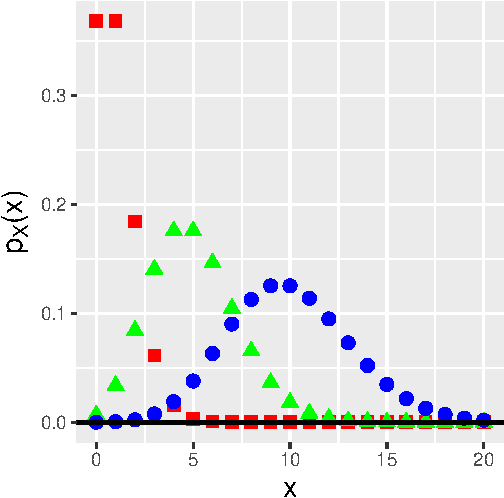
\includegraphics[keepaspectratio]{04-poisson_files/figure-latex/fig-ppmf-1.pdf}}

}

\caption{\label{fig-ppmf}Poisson probability mass functions for
\(\lambda = 1\) (red squares), 5 (green triangles), and 10 (blue
circles). Note how the shape of the pmf tends more and more towards that
of a normal distribution as \(\lambda\) gets larger.}

\end{figure}%

\subsection{Examples}\label{examples-37}

\subsubsection{Poisson Random Variable: Expected
Value}\label{poisson-random-variable-expected-value}

\smallskip\hrule

\begin{quote}
\textbf{Recall:} \emph{the expected value of a discretely distributed
random variable is} \[
E[X] = \sum_x x p_X(x) \,,
\] \emph{where the sum is over all values of \(x\) within the domain of
the pmf p\_X(x). The expected value is equivalent to a weighted average,
with the weight for each possible value of \(x\) given by \(p_X(x)\).}
\end{quote}

\smallskip\hrule

\begin{quote}
For a Poisson distribution, the expected value is \[
E[X] = \sum_{x=0}^\infty x \frac{\lambda^x}{x!} e^{-\lambda} = \sum_{x=1}^\infty x \frac{\lambda^x}{x!} e^{-\lambda} = \sum_{x=1}^\infty \frac{\lambda^x}{(x-1)!} e^{-\lambda} \,.
\] The trick here is to move constants into or out of the summation so
that the summation becomes one of a probability mass function over its
entire domain. Here, we move \(\lambda\) out of the summation, and make
the substitution \(y = x-1\); the summand then takes on the form of a
Poisson pmf, summed over its entire domain: \[
E[X] = \lambda \sum_{x=1}^\infty \frac{\lambda^{x-1}}{(x-1)!} e^{-\lambda} = \lambda \sum_{y=0}^\infty \frac{\lambda^{y}}{y!} e^{-\lambda} = \lambda \,.
\]
\end{quote}

\smallskip\hrule

\begin{quote}
\textbf{Recall:} \emph{the variance of a discretely distributed random
variable is} \[
V[X] = \sum_x (x-\mu)^2 p_X(x) = E[X^2] - (E[X])^2\,,
\] \emph{where the summation is over all values of \(x\) within the
domain of the pmf \(p_X(x)\). The variance represents the square of the
``width'' of a probability mass function, where by ``width'' we mean the
range of values of \(x\) for which \(p_X(x)\) is effectively non-zero.}
\end{quote}

\smallskip\hrule

\begin{quote}
A similar calculation to the one above, but that starts with the
derivation of the factorial moment \(E[X(X-1)]\), eventually yields the
Poisson variance, which is also \(\lambda\).
\end{quote}

\subsubsection{Poisson Distribution: Normal
Approximation}\label{poisson-distribution-normal-approximation}

\begin{quote}
As the expected number of counts, \(\lambda\), increases, a Poisson
random variable will converge in distribution to a normal random
variable. Here, we show mathematically why this is the case.
\end{quote}

\begin{quote}
The Poisson probability mass function is \[
p_X(x \vert \lambda) = \frac{\lambda^x}{x!} e^{-\lambda} \,.
\] We note that the normal probability density function does not have a
factorial in it, so we will start by using Stirling's approximation: \[
x! \approx \sqrt{2 \pi x} x^x e^{-x} \,.
\] This approximation has an error of 1.65\% for \(x = 5\) and 0.83\%
for \(x = 10\), with the percentage error continuing to shrink as
\(x \rightarrow \infty\). With this approximation, we can write that \[ 
p_X(x \vert \lambda) \approx \frac{\lambda^x}{\sqrt{2 \pi x}} x^{-x} e^{x-\lambda} \,.
\] This still does not quite look like a normal pdf. So there is more
work to do. We compute the logarithm of this quantity: \begin{align*}
\log p_X(x \vert \lambda) &\approx x \log \lambda - \frac{1}{2} \log (2 \pi x) - x \log x + x - \lambda \\
&= -x ( \log x - \log \lambda ) - \frac{1}{2} \log (2 \pi x) + x - \lambda \,,
\end{align*} and then look at \(\log x - \log \lambda\): \[
\log x - \log \lambda = \log \frac{x}{\lambda} = \log \left( 1 - \frac{\lambda-x}{\lambda}\right) \approx -\frac{\delta}{\sqrt{\lambda}} - \frac{\delta^2}{2 \lambda} - \cdots \,.
\] Here, \(\delta = (\lambda - x)/\sqrt{\lambda}\). Plugging this result
into the expression for \(\log p_X(x \vert \lambda)\), we find that \[
\log p_X(x \vert \lambda) \approx -\frac{1}{2} \log (2 \pi x) + x \left( \frac{\delta}{\sqrt{\lambda}} + \frac{\delta^2}{2\lambda} \right) - \delta \sqrt{\lambda} \,.
\] The next step is plug in \(x = \lambda - \sqrt{\lambda}\delta\):
\begin{align*}
\log p_X(x \vert \lambda) &\approx -\frac{1}{2} \log (2 \pi x) + (\lambda - \sqrt{\lambda}\delta)\left( \frac{\delta}{\sqrt{\lambda}} + \frac{\delta^2}{2\lambda} \right) - \delta \sqrt{\lambda} \\
&= -\frac{1}{2} \log (2 \pi x) + \sqrt{\lambda}\delta - \delta^2 + \frac{\delta^2}{2} - \frac{\delta^3}{2 \lambda^{3/2}} - \sqrt{\lambda}\delta \\
&\approx -\frac{1}{2} \log (2 \pi x) - \frac{\delta^2}{2} \,,
\end{align*} where we drop the \(\mathcal{O}(\delta^3)\) term. When we
exponentiate both sides, the final result is \[
p_X(x \vert \lambda) \approx \frac{1}{\sqrt{2 \pi x}} \exp\left( -\frac{\delta^2}{2} \right) = \frac{1}{\sqrt{2 \pi x}} \exp\left( -\frac{(x-\lambda)^2}{2\sqrt{\lambda}} \right) \,.
\] This has the (approximate) form of a normal pdf, at least for values
\(x \approx \lambda\). So, in the end, the Poisson probability mass
function \(p_X(x \vert \lambda)\) has approximately the same shape as
the normal probability density function
\(f_X(x \vert \mu=\lambda,\sigma^2=\lambda)\) for \(x \gg 1\) and
\(x \approx \lambda\).
\end{quote}

\subsubsection{Poisson Distribution: Exponential
Family}\label{poisson-distribution-exponential-family}

\smallskip\hrule

\begin{quote}
\textbf{Recall:} \emph{the exponential family of distributions is the
set of distributions whose probability mass or density functions can be
expressed as} \[ 
h(x) \exp\left[\left(\sum_{i=1}^p \eta_i(\boldsymbol{\theta}) T_i(x)\right) - A(\boldsymbol{\theta})\right] \,,
\] \emph{where \(\boldsymbol{\theta}\) is a vector of parameters (e.g.,
\(\boldsymbol{\theta} = \{\mu,\sigma^2\}\) for a normal distribution).
Note that none of the parameters can be a domain-specifying parameter.}
\end{quote}

\smallskip\hrule

\begin{quote}
Is the Poisson distribution a member of the larger exponential family of
distributions? We will start our answer to this question by noting that
\begin{align*}
\lambda^x = \exp\left(\log \lambda^x\right) = \exp\left(x \log \lambda\right) \,.
\end{align*} Thus \begin{align*}
p_X(x) = \frac{1}{x!} \exp\left(x \log \lambda - \lambda\right) \,.
\end{align*} and \begin{align*}
h(x) &= \frac{1}{x!} ~~~~~~ \eta(\lambda) = \log \lambda ~~~~~~ T(x) = x ~~~~~~ A(\lambda) = \lambda \,. 
\end{align*} The Poisson distribution is indeed a member of the
exponential family.
\end{quote}

\section{Poisson Distribution: Cumulative Distribution
Function}\label{sec-chap4cdf}

What to take away from this section:

\begin{itemize}
\tightlist
\item
  The cumulative distribution function, or cdf, for a Poisson
  distribution is a \emph{step function} that can be difficult to work
  with analytically (which historically motivated the application of the
  normal approximation, but which now leads us to use coding for exact
  inference).
\end{itemize}

\smallskip\hrule

\begin{quote}
\textbf{Recall}: \emph{the cumulative distribution function, or cdf, is
another means by which to encapsulate information about a probability
distribution. For a discrete distribution, it is defined as
\(F_X(x) = \sum_{y\leq x} p_Y(y)\), and it is defined for all values
\(x \in (-\infty,\infty)\), with \(F_X(-\infty) = 0\) and
\(F_X(\infty) = 1\).}
\end{quote}

\smallskip\hrule

For the Poisson distribution, the cdf is \[
F_X(x) = \sum_{y=0}^{\lfloor x \rfloor} p_Y(y) = \sum_{y=0}^{\lfloor x \rfloor} \frac{\lambda^y}{y!} \exp(-\lambda) = \frac{\Gamma(\lfloor x+1 \rfloor,\lambda)}{\lfloor x \rfloor !} \,,
\] where \(\lfloor x \rfloor\) denotes the floor function, which returns
the largest integer that is less than or equal to \(x\) (e.g., if \(x\)
= 8.33, \(\lfloor x \rfloor\) = 8), and where \(\Gamma(\cdot,\cdot)\) is
the upper incomplete gamma function \[
\Gamma(\lfloor x+1 \rfloor,\lambda) = \int_{\lambda}^\infty u^{\lfloor x \rfloor} e^{-u} du \,.
\] (An example of an \texttt{R} function which computes the upper
incomplete gamma function is \texttt{incgam()} in the \texttt{pracma}
package.) As we are dealing with a probability mass function, the cdf is
a step function, as illustrated in the left panel of
Figure~\ref{fig-poicdf}. Recall that because of the step-function nature
of the cdf, the form of inequalities in a probabilistic statement
matter: e.g., \(P(X < x)\) and \(P(X \leq x)\) will not be the same if
\(x\) is zero or a positive integer.

\smallskip\hrule

\begin{quote}
\textbf{Recall}: \emph{an inverse cdf function \(x = F_X^{-1}(q)\) takes
as input a distribution quantile \(q \in [0,1]\) and returns the value
of \(x\). A discrete distribution has no unique inverse cdf; it is
convention to utilize the generalized inverse cdf,} \[
x = \mbox{inf}\{x : F_X(x) \geq q\} \,,
\] \emph{where ``inf'' indicates that the function is to return the
smallest value of \(x\) such that \(F_X(x) \geq q\).}
\end{quote}

\smallskip\hrule

In the right panel of Figure~\ref{fig-poicdf}, we display the inverse
cdf for the same distribution used to generate the figure in the left
panel (\(\lambda = 2\)). Like the cdf, the inverse cdf for a discrete
distribution is a step function.

\begin{figure}

\centering{

\centering{

\pandocbounded{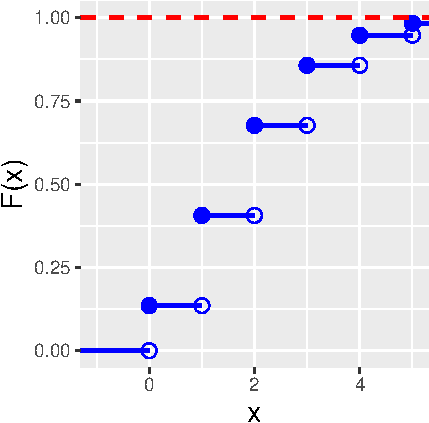
\includegraphics[keepaspectratio]{04-poisson_files/figure-latex/fig-poicdf-1.pdf}}

}

\subcaption{\label{fig-poicdf-1}}

\centering{

\pandocbounded{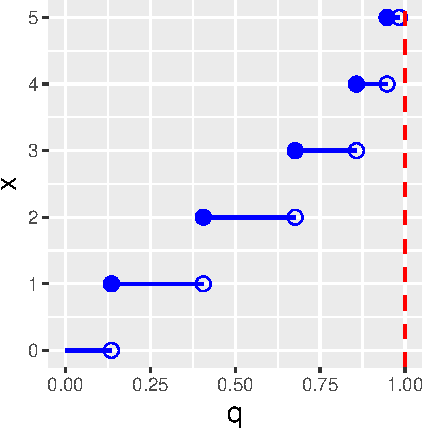
\includegraphics[keepaspectratio]{04-poisson_files/figure-latex/fig-poicdf-2.pdf}}

}

\subcaption{\label{fig-poicdf-2}}

}

\caption{\label{fig-poicdf}Illustration of the cumulative distribution
function \(F_X(x)\) (a) and inverse cumulative distribution function
\(F_X^{-1}(q)\) (b) for a Poisson distribution with \(\lambda=2\). Note
that because the domain of the Poisson distribution is countably
infinite, we do observe any values of \(x\) for which \(F_X(x) = 1\).}

\end{figure}%

\subsection{Example}\label{example-5}

\subsubsection{Computing Probabilities}\label{computing-probabilities-9}

\begin{quote}
\begin{enumerate}
\def\labelenumi{\arabic{enumi}.}
\tightlist
\item
  If \(X \sim\) Poisson(5), which is \(P(4 \leq X < 6)\)?
\end{enumerate}
\end{quote}

\begin{quote}
We first note that due to the form of the inequality, we do \emph{not}
include \(X=6\) in the computation. Thus
\(P(4 \leq X < 6) = p_X(4) + p_X(5)\), which equals \[
\frac{5^4}{4!}e^{-5} + \frac{5^5}{5!}e^{-5} = \frac{5^4}{4!}e^{-5} \left( 1 + \frac{5}{5} \right) = 2\frac{5^4}{4!}e^{-5} = 0.351\,.
\] If we utilize \texttt{R}:
\end{quote}

\begin{Shaded}
\begin{Highlighting}[]
\FunctionTok{round}\NormalTok{(}\FunctionTok{dpois}\NormalTok{(}\DecValTok{4}\NormalTok{, }\AttributeTok{lambda =} \DecValTok{5}\NormalTok{) }\SpecialCharTok{+} \FunctionTok{dpois}\NormalTok{(}\DecValTok{5}\NormalTok{, }\AttributeTok{lambda =} \DecValTok{5}\NormalTok{), }\DecValTok{3}\NormalTok{)}
\end{Highlighting}
\end{Shaded}

\begin{verbatim}
[1] 0.351
\end{verbatim}

\begin{quote}
Note that we can take advantage of \texttt{R}'s vectorization
capabilities by writing the above as
\end{quote}

\begin{Shaded}
\begin{Highlighting}[]
\FunctionTok{round}\NormalTok{(}\FunctionTok{sum}\NormalTok{(}\FunctionTok{dpois}\NormalTok{(}\DecValTok{4}\SpecialCharTok{:}\DecValTok{5}\NormalTok{, }\AttributeTok{lambda =} \DecValTok{5}\NormalTok{)), }\DecValTok{3}\NormalTok{)}
\end{Highlighting}
\end{Shaded}

\begin{verbatim}
[1] 0.351
\end{verbatim}

\begin{quote}
This approach is far more convenient than writing out a string of calls
to \texttt{dpois()}, particularly when the number of values of \(x\) to
sum over becomes large. We can also utilize cdf functions here:
\begin{align*}
P(4 \leq X < 6) &= P(X < 6) - P(X < 4) = P(X \leq 5) - P(X \leq 3)\\
&= F_X(5) - F_X(3) \,,
\end{align*} which in \texttt{R} is computed as follows:
\end{quote}

\begin{Shaded}
\begin{Highlighting}[]
\FunctionTok{round}\NormalTok{(}\FunctionTok{ppois}\NormalTok{(}\DecValTok{5}\NormalTok{, }\AttributeTok{lambda =} \DecValTok{5}\NormalTok{) }\SpecialCharTok{{-}} \FunctionTok{ppois}\NormalTok{(}\DecValTok{3}\NormalTok{, }\AttributeTok{lambda =} \DecValTok{5}\NormalTok{), }\DecValTok{3}\NormalTok{)}
\end{Highlighting}
\end{Shaded}

\begin{verbatim}
[1] 0.351
\end{verbatim}

\begin{quote}
However, summing pmf values is the preferred approach, as this approach
makes it easier to properly take into account the form of any
inequalities in a probability statement.
\end{quote}

\begin{quote}
\begin{enumerate}
\def\labelenumi{\arabic{enumi}.}
\setcounter{enumi}{1}
\tightlist
\item
  If \(X \sim\) Poisson(5), what is the value of \(a\) such that
  \(P(X \leq a) = 0.9\)?
\end{enumerate}
\end{quote}

\begin{quote}
First, we set up the inverse cdf formula: \[
P(X \leq a) = F_X(a) = 0.9 ~~~ \Rightarrow ~~~ a = F_X^{-1}(0.9)
\] Note that we do not do anything differently here than we would have
done in a continuous distribution setting\ldots and we can proceed
directly to \texttt{R} because it utilizes the generalized inverse cdf
algorithm.
\end{quote}

\begin{Shaded}
\begin{Highlighting}[]
\FunctionTok{qpois}\NormalTok{(}\FloatTok{0.9}\NormalTok{, }\AttributeTok{lambda =} \DecValTok{5}\NormalTok{)}
\end{Highlighting}
\end{Shaded}

\begin{verbatim}
[1] 8
\end{verbatim}

\section{Poisson-Related Distributions}\label{sec-chap4related}

What to take away from this section:

\begin{itemize}
\item
  There are several distributions related to the Poisson distribution
  that are often seen in data analyses\ldots{}

  \begin{itemize}
  \item
    the \emph{zero-inflated Poisson} distribution, a model that takes
    into account the fact that a data-generating process might include
    observing a heightened number of zero-count outcomes;
  \item
    the \emph{zero-truncated Poisson} distribution, a model that takes
    into account the fact that a data-generating process might be such
    that it is impossible to observe a zero-count outcomes; and
  \item
    the \emph{gamma} distribution, a continuous semi-infinite
    distribution that one can use to model the Poisson expected counts
    \(\lambda\).
  \end{itemize}
\end{itemize}

There are several probability distributions that are directly related to
the Poisson distribution and that are commonly utilized in statistical
inference. Some of these are

\begin{itemize}
\tightlist
\item
  the \emph{zero-inflated Poisson} distribution;
\item
  the \emph{zero-trucated Poisson} distribution; and
\item
  the \emph{gamma} distribution.
\end{itemize}

Below, we introduce each in turn.

\subsection{Zero-Inflated Poisson Distribution}\label{sec-chap4zeroinf}

The experimental setting for this distribution is a simple one: when
counting the numbers of a particular object (like an animal species)
that exist at different locations and/or times, it can be the case that
the object in question only exists in a subset of those
locations/times\ldots meaning that we might record a larger number of
zeros than we might expect, and thus that we should not model the data
with a conventional Poisson distribution. In a zero-inflated Poisson (or
ZIP) process, data are assumed to be sampled according to a mixture of
\emph{two} distributions:

\begin{enumerate}
\def\labelenumi{\arabic{enumi}.}
\tightlist
\item
  a distribution that generates only zeros; and
\item
  a Poisson distribution
\end{enumerate}

The probability mass function for the ZIP distribution is \[
p_X(x) = \left\{ \begin{array}{ll} \theta + (1-\theta) e^{-\lambda} & x = 0 \\ (1 - \theta) \frac{\lambda^x}{x!} e^{-\lambda} & x \in \{1,2,\ldots\} \end{array} \right. \,,
\] where \(\lambda > 0\) and \(\theta \in [0,1]\).

\subsection{Zero-Truncated Poisson
Distribution}\label{sec-chap4zerotrunc}

In contrast to situations in which we might invoke the zero-inflated
Poisson distribution, there can be experimental settings in which the
data are counts but zero is not a possibility. For instance, if our data
are the number of items purchased across \(n\) separate online orders,
presumably none of the \(n\) values will be zero: one cannot make a
purchase without at least one item in the cart!

The zero-truncated Poisson distribution is also known as the conditional
Poisson distribution, and that alternative name makes sense, as we can
derive the probability mass function for the ZTP distribution by
computing \(P(X = x \vert X > 0)\), where \(X\) is a(n uncoditional)
Poisson random variable: \begin{align*}
p_X(x) = P(X = x \vert X > 0) &= \frac{P(X = x \cap X > 0)}{P(X > 0)} \\
&= \frac{P(X = x \cap X > 0)}{1 - P(X = 0)} \\
&= \frac{P(X = x)}{1 - P(X = 0)} \\
&= \frac{\lambda^x}{x!}e^{-\lambda}\frac{1}{1 - e^{-\lambda}} \\
&= \frac{\lambda^x}{x! (e^\lambda - 1)} \,,
\end{align*} where \(x \in \{1,\ldots\}\) and \(\lambda > 0\).

\subsection{Gamma Distribution}\label{sec-chap4gamma}

The gamma distribution is a continuous distribution that is commonly
used to, e.g., model the waiting times between discrete events. (Recall
that we have previously encountered this distribution: given \(n\) iid
normal random variables, \(S^2\) is a gamma-distributed random
variable.) Its probability density function is given by \[
f_X(x) = \frac{x^{a-1}}{b^a} \frac{\exp\left(-x/b\right)}{\Gamma(a)} \,,
\] where \(x \in [0,\infty)\), \(a\) and \(b\) are both \(>\) 0, and
\(\Gamma(a)\) is the gamma function: \[
\Gamma(a) = \int_0^\infty u^{a-1} e^{-u} du \,.
\] (See Figure~\ref{fig-gammapdf}.) \(a\) and \(b\) are referred to as
``shape'' and ``scale'' parameters, respectively. (Note that there is an
alternative parameterization of the gamma distribution, the so-called
``shape/rate'' parameterization. So one should always be careful to
determine which parameterization that one is working with before
performing any analyses.) The gamma family of distributions exhibits a
wide variety of shapes and it is the parent family to a number of other
distributions, some of which we have met before. One in particular is
the \emph{exponential distribution}, \[
f_X(x) = \frac{1}{b} \exp\left(-\frac{x}{b}\right) \,,
\] which is a gamma distribution with \(a = 1\). Note how we lead off
above by saying that the gamma distribution is commonly used to model
the waiting times between discrete events. The exponential distribution
specifically models the waiting time between one event and the next in a
homogeneous Poisson process (i.e., one in which \(\lambda\) does not
vary as a function of time). The number of strong earthquakes that occur
in California in one year? That can be modeled as a Poisson random
variable. The time that elapses between two consecutive strong
earthquakes in California? That can be modeled using the exponential
distribution. (For completeness: the Erlang distribution is a
generalization of the exponential distribution, in the sense that we can
use it to model the waiting time between the \(i^{\mathrm{th}}\) and
\((i+a)^{\mathrm{th}}\) events, where \(a\) is a positive integer, in a
Poisson process.)

{\def\LTcaptype{none} % do not increment counter
\begin{longtable}[]{@{}rcc@{}}
\toprule\noalign{}
distribution & \(a\) & \(b\) \\
\midrule\noalign{}
\endhead
\bottomrule\noalign{}
\endlastfoot
exponential & 1 & \((0,\infty)\) \\
Erlang & \(\{1,2,3,\ldots\}\) & \((0,\infty)\) \\
chi-square & \(\{1/2,1,3/2,\ldots\}\) & 2 \\
\end{longtable}
}

Let's conclude this section by repeating the exercise we performed in
Section~\ref{sec-chap3beta} when discussing the beta distribution, the
one in which we examined the functional form of the likelihood function
\(\mathcal{L}(p \vert k,x)\). Here, we write down the Poisson likelihood
function \[
\mathcal{L}(\lambda \vert x) = \frac{\lambda^x}{x!} e^{-\lambda}
\] and compare it with the gamma pdf. We can match the gamma pdf if we
map the Poisson \(\lambda\) to the gamma \(x\), the Poisson \(x\) to the
gamma \(a-1\), and we set \(b\) to 1. But because the Poisson \(x\) is
an integer with values \(\{0,1,2,\ldots\}\), we find that the integrand
specifically matches the Erlang pdf, for which \(a = \{1,2,3,\ldots\}\).
So, if we observe a random variable \(X \sim\) Poisson(\(\lambda\)),
then the likelihood function \(\mathcal{L}(\lambda \vert x)\) has the
shape (and normalization!) of a Gamma(\(x+1,1\)) (or Erlang(\(x+1\)))
distribution.

(About the normalization: if we integrate the likelihood function over
its domain, we find that \[
\frac{1}{x!} \int_0^\infty \lambda^x e^{-\lambda} d\lambda = \frac{1}{x!} \Gamma(x+1) = \frac{x!}{x!} = 1 \,.
\] The mathematics works out here because \(x\) is integer valued and
thus \(\Gamma(x+1) = x!\).)

\begin{figure}

\centering{

\pandocbounded{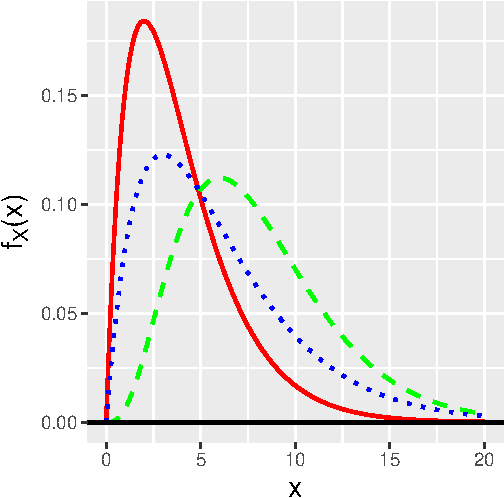
\includegraphics[keepaspectratio]{04-poisson_files/figure-latex/fig-gammapdf-1.pdf}}

}

\caption{\label{fig-gammapdf}Three examples of gamma probability density
functions: Gamma(2, 2) (solid red line), Gamma(4, 2) (dashed green
line), and Gamma(2, 3) (dotted blue line).}

\end{figure}%

\subsection{Examples}\label{examples-38}

\subsubsection{Zero-Inflated Poisson Random Variable: Expected
Value}\label{zero-inflated-poisson-random-variable-expected-value}

\begin{quote}
The zero-inflated Poisson, or ZIP, distribution has probability mass
function \[
p_X(x) = \left\{ \begin{array}{ll} \theta + (1-\theta) e^{-\lambda} & x = 0 \\ (1 - \theta) \frac{\lambda^x}{x!} e^{-\lambda} & x = \{1,2,\ldots\} \end{array} \right.
\] Thus the expected value is \begin{align*}
E[X] = \sum_{x=0}^\infty x p_X(x) &= 0 + \sum_{x=1}^\infty x(1-\theta)\frac{\lambda^x}{x!} e^{-\lambda} \\
&= \sum_{x=1}^\infty (1-\theta)\frac{\lambda^x}{(x-1)!} e^{-\lambda} \\
&= \lambda (1-\theta) \sum_{x=1}^\infty \frac{\lambda^{x-1}}{(x-1)!} e^{-\lambda} \\
&= \lambda (1-\theta) \sum_{y=0}^\infty \frac{\lambda^y}{y!} e^{-\lambda} \\
&= \lambda (1-\theta) \,.
\end{align*} The variance, which one can derive by working with the
second factorial moment \(E[X(X-1)]\), is
\(\lambda (1-\theta) (1 + \lambda\theta)\).
\end{quote}

\subsubsection{Zero-Truncated Poisson Random Variable: Expected
Value}\label{zero-truncated-poisson-random-variable-expected-value}

\begin{quote}
The zero-truncated Poisson, or ZTP, distribution has probability mass
function \[
p_X(x) = \frac{\lambda^x}{x! (e^\lambda-1)} \,,
\] where \(x \in \{1,\ldots\}\) and \(\lambda > 0\). The expected value
is thus \begin{align*}
E[X] &= \sum_{x=1}^\infty x p_X(x) \\
&= \frac{1}{e^\lambda-1} \sum_{x=1}^\infty x \frac{\lambda^x}{x!} \\
&= \frac{1}{e^\lambda-1} \sum_{x=1}^\infty \frac{\lambda^x}{(x-1)!} \\
&= \frac{\lambda}{e^\lambda-1} \sum_{x=1}^\infty \frac{\lambda^{x-1}}{(x-1)!} \\
&= \frac{\lambda e^\lambda}{e^\lambda-1} \sum_{x=1}^\infty \frac{\lambda^{x-1}}{(x-1)!} e^{-\lambda} \\
&= \frac{\lambda e^\lambda}{e^\lambda-1} \sum_{y=0}^\infty \frac{\lambda^y}{y!} e^{-\lambda} \\
&= \frac{\lambda e^\lambda}{e^\lambda-1} = \frac{\lambda}{1-e^{-\lambda}} \,.
\end{align*} The variance, which one can derive by working with the
second factorial moment \(E[X(X-1)]\), is \[
V[X] = \frac{\lambda [ 1 - (\lambda+1) e^{-\lambda} ]}{(1-e^{-\lambda})^2} \,.
\]
\end{quote}

\subsubsection{Gamma Random Variable: Expected
Value}\label{gamma-random-variable-expected-value}

\begin{quote}
The expected value of a gamma random variable is found by introducing
constants into the expected value integral so that a gamma pdf integrand
is formed. Specifically \begin{align*}
E[X] = \int_0^\infty x f_X(x) dx &= \int_0^\infty x \frac{x^{a-1}}{b^a} \frac{\exp(-x/b)}{\Gamma(a)} dx \\
&= \int_0^\infty \frac{x^{a}}{b^a} \frac{\exp(-x/b)}{\Gamma(a)} dx \\
&= \int_0^\infty \frac{x^{a}}{b^a} \frac{\exp(-x/b)}{\Gamma(a)} \frac{\Gamma(a+1)}{\Gamma(a+1)} \frac{b^{a+1}}{b^{a+1}} dx \\
&= \int_0^\infty \frac{x^{a}}{b^{a+1}} \frac{\exp(-x/b)}{\Gamma(a+1)} \frac{\Gamma(a+1)}{\Gamma(a)} \frac{b^{a+1}}{b^a} dx \\
&= \frac{\Gamma(a+1)}{\Gamma(a)} \frac{b^{a+1}}{b^a} \int_0^\infty \frac{x^{a}}{b^{a+1}} \frac{\exp(-x/b)}{\Gamma(a+1)} dx \\
&= \frac{a \Gamma(a)}{\Gamma(a)} b \times 1 \\
&= a b \,.
\end{align*} By introducing the constants, we are able to transform the
integrand to that of a Gamma(\(a+1,b\)) distribution, and because the
integral is over the entire domain of a gamma distribution, the integral
evaluates to 1.
\end{quote}

\begin{quote}
A similar calculation involving the derivation of \(E[X^2]\) allows us
to determine that the variance of a gamma random variable is
\(V[X] = a b^2\).
\end{quote}

\subsubsection{Exponential Distribution:
Memorylessness}\label{exponential-distribution-memorylessness}

\begin{quote}
An important feature of the exponential distribution is that when we use
it to model, e.g., the lifetimes of components in a system, it exhibits
\emph{memorylessness}. In other words, if \(T\) is the random variable
representing a component's lifetime, where \(T \sim\) Exponential(\(b\))
and where \(E[T] = b\), it doesn't matter how old the component is when
we first examine it: \emph{from that point onward}, the average lifetime
will be \(b\).
\end{quote}

\begin{quote}
Let's demonstrate how this works. We examine a component ``born'' at
time \(t_0=0\) at a later time \(t_1\), and we wish to determine the
probability that it will live beyond an even later time \(t_2\). In
other words, we wish to compute \[
P(T \geq t_2-t_0 \vert T \geq t_1-t_0) \,.
\] (We know the component lived to time \(t_1\), hence the added
condition.) Let \(T \sim\) Exponential(\(b\)). Then \begin{align*}
P(T \geq t_2-t_0 \vert T \geq t_1-t_0) &= \frac{P(T \geq t_2-t_0 \cap T \geq t_1-t_0)}{P(T \geq t_1-t_0)} \\
&= \frac{P(T \geq t_2-t_0)}{P(T \geq t_1-t_0)} \\
&= \frac{\int_{t_2-t_0}^\infty (1/b) \exp(-t/b) dt}{\int_{t_1-t_0}^\infty (1/b) \exp(-t/b) dt} \\
&= \frac{\left. -\exp(-t/b) \right|_{t_2-t_0}^\infty}{\left. -\exp(-t/b) \right|_{t_1-t_0}^\infty} \\
&= \frac{0 + \exp(-(t_2-t_0)/b)}{0 + \exp(-(t_1-t_0)/b)} \\
&= \exp[-(t_2-t_1)/b] = P(T \geq t_2-t_1) \,.
\end{align*} Note that \(t_0\) drops out of the final result: no matter
how long ago \(t_0\) might have been, the probability that the component
will live \(t_2-t_1\) units longer is the same, and the average
additional lifetime is still \(b\).
\end{quote}

\section{Linear Functions of Poisson Random
Variables}\label{sec-chap4linear}

What to take away from this section:

\begin{itemize}
\item
  The \emph{method of moment-generating functions} allows us to
  determine that\ldots{}

  \begin{itemize}
  \item
    the sum of \(n\) iid Poisson random variables is itself Poisson
    distributed; and
  \item
    the mean of \(n\) iid binomial random variables has a known but
    typically unutilized distribution: it is the sample sum distribution
    with a transformed domain.
  \end{itemize}
\item
  Foreshadowing: the sample sum result will allow us to make statistical
  inferences about the Poisson expected counts parameter \(\lambda\),
  given \(n\) iid normal random variables.
\end{itemize}

For previous material on sampling distributions, see
Section~\ref{sec-chap2methodmgf}.

Let's assume we are given \(n\) iid Poisson random variables:
\(X_1,X_2,\ldots,X_n \sim\) Poisson(\(\lambda\)). What is the
distribution of \(Y = \sum_{i=1}^n a_i X_i\)?

\smallskip\hrule

\begin{quote}
\textbf{Recall}: \emph{the moment-generating function, or mgf, is a
means by which to encapsulate information about a probability
distribution. When it exists, the mgf is given by
\(m_X(t) = E[e^{tX}]\). Also, if \(Y = \sum_{i=1}^n a_iX_i\), then
\(m_Y(t) = m_{X_1}(a_1t) m_{X_2}(a_2t) \cdots m_{X_n}(a_nt)\); if we can
identify \(m_Y(t)\) as the mgf for a known family of distributions, then
we can immediately identify the distribution for \(Y\) and the
parameters of that distribution.}
\end{quote}

\smallskip\hrule

If \(X\) is a Poisson random variable, then \begin{align*}
m_X(t) = E[e^{tX}] &= \sum_{x=0}^\infty e^{tx} p_X(x) = \sum_{x=0}^\infty e^{tx} \frac{\lambda^x}{x!} e^{-\lambda} = e^{-\lambda} \sum_{x=0}^\infty \frac{\lambda^x}{x!} e^{tx} \\
&= e^{-\lambda} \left[ 1 + \lambda e^t + \frac{\lambda^2}{2!}e^{2t} + \ldots \right] = e^{-\lambda} \left[ 1 + y + \frac{y^2}{2!} + \ldots \right] \\
&= e^{-\lambda} e^y = \exp(-\lambda) \exp(\lambda e^t) = \exp[\lambda(e^t-1)] \,.
\end{align*} Thus the mgf for \(Y = \sum_{i=1}^n X_i\) is \begin{align*}
m_Y(t) &= \exp\left[\lambda\left(e^t-1\right)\right] \cdots \exp\left[\lambda\left(e^t-1\right)\right]\\
&= \exp\left[(\lambda+\cdots+\lambda)(e^t-1)\right] = \exp\left[n\lambda(e^t-1)\right] \,.
\end{align*} This mgf retains the form of a Poisson mgf. We thus see
that the sum of \(n\) iid Poisson-distributed random variables is itself
Poisson distributed with parameter \(n\lambda\), i.e.,
\(Y = \sum_{i=1}^n X_i \sim\) Poisson(\(n\lambda\)).

As was the case for the binomial distribution, the sample mean of \(n\)
iid Poisson-distributed random variables has a sampling distribution
whose masses are identical to those observed for the sample sum, but
whose domain shifts from \(\{0,1,\cdots\}\) to \(\{0,1/n,\cdots\}\). (As
a reminder, we can derive this result mathematically by making the
general transformation
\(\sum_{i=1}^n X_i \rightarrow (\sum_{i=1}^n X_i)/n\).) While we could
define, e.g., the sample mean pmf ourselves using our own \texttt{R}
function, there is no real need to: e.g., if we wish to construct a
confidence interval for \(\lambda\), we can simply construct one for
\(n\lambda\) using the sum of the data as a statistic, and then divide
each bound by \(n\). (We could also, in theory, utilize the Central
Limit Theorem if \(n \gtrsim 30\), but there is absolutely no reason to
do that to make inferences about \(\lambda\): we know the distribution
of the sum of the data exactly, and thus there is no need to fall back
upon approximations.)

\subsection{Examples}\label{examples-39}

\subsubsection{Two Poisson Random Variables: Difference
Distribution}\label{two-poisson-random-variables-difference-distribution}

\begin{quote}
Let's assume that we are pointing a camera at an object, such as a star.
A star gives off photons at a particular average rate \(r_S\) (with
units of, e.g., photons per second). Thus if we open the shutter for a
length of time \(t\), the number of photons we observe from the star is
a Poisson random variable \(S \sim\) Poisson(\(\lambda_S=r_St\)). But
the star is not the only object in the field of view; there may be other
objects in the background that give off photons at a rate \(r_B\), and
the number of photons we observe from the background will be \(B \sim\)
Poisson(\(\lambda_B=r_Bt\)). Thus what we record is not \(S\), but
\(T = S+B\)\ldots so how can we make statistical inferences about \(S\)
itself?
\end{quote}

\begin{quote}
One possibility is to point the camera to an ``empty'' field near the
star, and record some number of photons \(B\) over the same amount of
time. Then we can estimate \(S\) using \(S = T - B\). What is the
distribution of \(S\)?
\end{quote}

\begin{quote}
We can utilize the method of moment-generating functions and write that
\begin{align*}
m_S(t) = m_T(t) m_B(-t) &= \exp[\lambda_T(e^t-1)] \exp[\lambda_B(e^{-t}-1)] \\
&= \exp[\lambda_T(e^t-1) + \lambda_B(e^{-t}-1)] \\
&= \exp[-(\lambda_T+\lambda_B) + \lambda_Te^t + \lambda_Be^{-t}] \,,
\end{align*} where \(\lambda_T = \lambda_S+\lambda_B = (r_S+r_B)t\). At
first, utilizing the method of mgfs appears to be a fool's errand: this
is not an mgf we know. But it turns out that the family of distributions
associated with this mgf \emph{does} have a name: \(S = T-B\) is a
random variable sampled according to a \emph{Skellam distribution}, with
mean \(\lambda_T-\lambda_B\) and variance \(\lambda_T+\lambda_B\). We
can work with this distribution to, e.g., construct confidence intervals
for \(\mu_S\), etc., if we so choose. (Note, however, that in order to
do this we would need to fix \(\mu_B\)\ldots or we would have to move
into the realm of numerical confidence \emph{region} construction, which
is beyond the scope of this book.)
\end{quote}

\subsubsection{Zero-Inflated Poisson Distribution: Moment-Generating
Function}\label{zero-inflated-poisson-distribution-moment-generating-function}

\begin{quote}
Recall that the zero-inflated Poisson, or ZIP, distribution has
probability mass function \[
p_X(x) = \left\{ \begin{array}{ll} \theta + (1-\theta) e^{-\lambda} & x = 0 \\ (1 - \theta) \frac{\lambda^x}{x!} e^{-\lambda} & x = \{1,2,\ldots\} \end{array} \right.
\] If we have \(n\) iid data distributed according to a ZIP
distribution, can we determine the distribution of, e.g., the sample
sum?
\end{quote}

\begin{quote}
The moment-generating function for the ZIP distribution is
\begin{align*}
m_X(t) = E[e^{tX}] &= \sum_{x=0}^\infty e^{tx} p_X(x) \\
&= \theta + (1-\theta)e^{-\lambda} + \sum_{x=1}^\infty e^{tx} (1-\theta) \frac{\lambda^x}{x!} e^{-\lambda} \\
&= \theta + \sum_{x=0}^\infty e^{tx} (1-\theta) \frac{\lambda^x}{x!} e^{-\lambda} \\
&= \theta + (1-\theta) e^{-\lambda} \sum_{x=0}^\infty \frac{\lambda^x}{x!} e^{tx} \\
&= \theta + (1-\theta) \exp(-\lambda) \exp(\lambda e^t) = \theta + (1-\theta) \exp[\lambda(e^t-1)] \,.
\end{align*} We have already seen how to evaluate the final summation,
in an example just above.
\end{quote}

\begin{quote}
The mgf for, e.g., the sample sum is \[
m_Y(t) = \prod_{i=1}^n m_{X_i}(t) = \left[ m_X(t) \right]^n = \left[ \theta + (1-\theta) \exp[\lambda(e^t-1)] \right]^n \,.
\] It is clear that this is not the mgf of a ZIP distribution (or any
other distribution with which we are familiar). Hence any statistical
inference that we would wish to perform given ZIP-distributed data would
require us to utilize simulations. We show how to use simulations to,
e.g., construct confidence intervals in an example later, in
Section~\ref{sec-chap4confidence}.
\end{quote}

\begin{quote}
(We note, for completeness, that we run into the same issue with the
zero-truncated Poisson distribution. We can derive the mgf easily
enough\ldots{} \[
m_X(t) = \frac{\exp[\lambda(e^t-1)] - \exp(-\lambda)}{1 - \exp(-\lambda)}
\] \ldots but we cannot use it to derive an exact sampling distribution
for, e.g., the sample sum.)
\end{quote}

\subsubsection{Exponential Data: Sample Sum
Distribution}\label{exponential-data-sample-sum-distribution}

\begin{quote}
As stated above, the exponential distribution, i.e., the gamma
distribution with \(\alpha = 1\), is used to model the waiting time
between two successive events in a Poisson process. Let's assume that we
have recorded \(n\) separate times between \(n\) separate pairs of
events. What is the distribution of \(T = T_1 + \cdots + T_n\)?
\end{quote}

\begin{quote}
As we do when faced with a linear function of \(n\) iid random
variables, we utilize the method of moment-generating functions: \[ 
m_T(t) = \prod_{i=1}^n m_{T_i}(t) \,,
\] where \(m_{T_i}(t) = (1-b t)^{-1}\) is the mgf for the exponential
distribution. Thus \[
m_T(t) = \prod_{i=1}^n (1-b t)^{-1} = (1-b t)^{-n} \,.
\] This has the form of the mgf for a Gamma(\(n,b\)) distribution, or,
equivalently, an Erlang(\(n,b\)) distribution. In other words the sum of
\(n\) iid waiting times has the same distribution as the waiting time
between the \(i^{\mathrm{th}}\) and \((i+n)^{\mathrm{th}}\) events of a
Poisson process.
\end{quote}

\section{Point Estimation}\label{sec-chap4point}

What to take away from this section:

\begin{itemize}
\item
  Along with the maximum likelihood estimator and the minimum variance
  unbiased estimator, there has historically been a third point
  estimator that practitioners have used: the \emph{method of moments}
  estimator or \emph{MoM} estimator.
\item
  The MoM estimator is useful when, e.g., we are trying to jointly
  estimate two or more parameter values, or when we are trying to
  estimate one value and we cannot analytically derive either the MLE or
  the MVUE.
\item
  A MoM estimator does not possess the invariance property, nor is there
  a guarantee that it converges in distribution to a normal random
  variable.
\item
  In the age of computers, the method of moments has been superseded by
  the use of numerical optimization to estimate the MLE.
\end{itemize}

For previous material on point estimation, see
Section~\ref{sec-chap3point}.

Previously, we described two commonly used point estimators: the maximum
likelihood estimator (or MLE) and the minimum variance unbiased
estimator (or MVUE). We review both below in examples, in the context of
estimating the Poisson \(\lambda\) parameter. Here, for completeness, we
introduce one last, less-commonly used approach, the so-called
\emph{method of moments} estimator.

\subsection{Method of Moments Estimation}\label{sec-chap4moments}

The \emph{method of moments} (or MoM) is a classic means by which to
define estimators that has been historically useful when we face with
the following situation: (a) the likelihood function is not easily
differentiated, because it contains terms like \(\Gamma(\theta)\); and
(b) the distribution has two or more free parameters, rendering it
difficult (though certainly not impossible) to define the MVUE, since we
would have to work with joint sufficient statistics and their
multivariate sampling distributions. Now, why do we say ``historically
useful''? Because in the age of computers, we can always determine MLEs
(or, at least, their numerical values) via numerical optimization (as
shown in an example below), which effectively eliminates any need to
ever use the MoM estimator in practice.

Recall that by definition, \(E[X^k]\) is the \(k^{\mathrm{th}}\) moment
of the distribution of the random variable \(X\). We can define
analagous \emph{sample moments}, e.g., \[
m_1 = \frac{1}{n} \sum_{i=1}^n X_i = \bar{X} ~~ \mbox{and} ~~ m_2 = \frac{1}{n} \sum_{i=1}^n X_i^2 = \overline{X^2} \,.
\] (For \(m_2\): note that the average of \(X_i^2\) is \emph{not} the
same as the average of \(X_i\), squared.) Let's suppose that we have
\(p\) parameters that we are trying to estimate. In method of moments
estimation, we generally set the first \(p\) population moments equal to
the first \(p\) sample moments and solve the system of equations to
determine parameter estimates. These estimates are generally consistent,
but also may be biased. (Situations may exist where higher-order moments
may be preferable to use, such as when the one parameter of a
distribution is \(\sigma^2\) and thus we might derive a better estimator
using the second moment rather than the first, but typically we use the
first \(p\) moments.)

For the Poisson distribution, there is one parameter to estimate and
thus we set \(\mu_1' = E[X] = \lambda = m_1' = \bar{X}\). We thus find
that \(\hat{\lambda}_{MoM} = \bar{X}\). For a more relevant example of
method of moments usage, see below.

For more on point estimation, go to Section~\ref{sec-chap5point}.

\subsection{Examples}\label{examples-40}

\subsubsection{Poisson Expected Counts: Maximum Likelihood
Estimator}\label{poisson-expected-counts-maximum-likelihood-estimator}

\smallskip\hrule

\begin{quote}
\textbf{Recall}: \emph{the value of \(\theta\) that maximizes the
likelihood function is the maximum likelihood estimate, or MLE, for
\(\theta\). The maximum is found by taking the (partial) derivative of
the (log-)likelihood function with respect to \(\theta\), setting the
result to zero, and solving for \(\theta\). That solution is the maximum
likelihood estimate \(\hat{\theta}_{MLE}\). Also recall the invariance
property of the MLE: if \(\hat{\theta}_{MLE}\) is the MLE for
\(\theta\), then \(g(\hat{\theta}_{MLE})\) is the MLE for
\(g(\theta)\).}
\end{quote}

\smallskip\hrule

\begin{quote}
The likelihood function for the Poisson parameter \(\lambda\) is \[
\mathcal{L}(\lambda \vert \mathbf{x}) = \prod_{i=1}^n \frac{\lambda^{x_i}}{x_i!} \exp(-\lambda)
\] and the log-likelihood is \[
\ell(\lambda \vert \mathbf{x}) = \left(\sum_{i=1}^n x_i\right) \log \lambda - n \lambda - \log\left(\prod_{i=1}^n x_i!\right) \,.
\] (Note that we could write this as \[
\ell(\lambda \vert \mathbf{x}) \propto \left(\sum_{i=1}^n x_i\right) \log \lambda - n \lambda \,,
\] where \(\propto\) is the proportionality symbol, because the last
term in the original log-likelihood will disappear during
differentiation because it does not contain \(\lambda\).) The derivative
of \(\ell(\lambda \vert \mathbf{x})\) with respect to \(\lambda\) is \[
\frac{d\ell}{d\lambda} = \left(\frac{1}{\lambda}\sum_{i=1}^n x_i \right) - n \,.
\] Setting the derivative to zero and rearranging terms, we find that \[
\hat{\lambda}_{MLE} = \frac{1}{n} \sum_{i=1}^n X_i = \bar{X}
\] is the MLE for \(\lambda\).
\end{quote}

\smallskip\hrule

\begin{quote}
\textbf{Recall}: \emph{the bias of an estimator is the difference
between the average value of the estimates it generates and the true
parameter value. If \(E[\hat{\theta}-\theta] = 0\), then the estimator
\(\hat{\theta}\) is said to be unbiased.}
\end{quote}

\smallskip\hrule

\begin{quote}
By the general rule for \(\bar{X}\) introduced in
Section~\ref{sec-chap1stat},
\(E[\hat{\lambda}_{MLE}] = E[\bar{X}] = \lambda\), so
\(\hat{\lambda}_{MLE}\) is an unbiased estimator. (There is no guarantee
that the MLE will always be an unbiased estimator\(-\)it just happens to
be so here\(-\)but it will always be at least asymptotically unbiased.)
\end{quote}

\smallskip\hrule

\begin{quote}
\textbf{Recall}: \emph{an estimator is consistent if its mean-squared
error, \(B[\hat{\theta}]^2 + V[\hat{\theta}]\), goes to zero as the
sample size \(n\) goes to infinity.}
\end{quote}

\smallskip\hrule

\begin{quote}
\(V[\hat{\lambda}_{MLE}] = \lambda/n\), so \(\hat{\lambda}_{MLE}\) is a
consistent estimator, since \(\hat{\lambda}_{MLE} \rightarrow \lambda\)
as \(n \rightarrow \infty\). (The MLE is always a consistent estimator.)
\end{quote}

\begin{quote}
If we wish to find the MLE for a function of the parameter, e.g.,
\(\lambda^2\), we simply apply that function to \(\hat{\theta}_{MLE}\).
Hence \(\hat{\lambda^2}_{MLE}\) is \(\bar{X}^2\). This is the invariance
property of the MLE.
\end{quote}

\begin{quote}
Last, recall that the MLE converges in distribution to a normal random
variable with mean \(\theta\) and variance \(1/I_n(\theta)\), where
\(I_n(\theta)\) is the Fisher information content of the data sample.
Here, that means that \[
\hat{\lambda} \overset{d}{\rightarrow} Y \sim \mathcal{N}\left(\lambda,\frac{\lambda}{n}\right) \,.
\]
\end{quote}

\subsubsection{Poisson Expected Counts: Minimum Variance Unbiased
Estimator}\label{poisson-expected-counts-minimum-variance-unbiased-estimator}

\smallskip\hrule

\begin{quote}
\textbf{Recall}: \emph{deriving the minimum variance unbiased estimator
involves two steps:}
\end{quote}

\begin{quote}
\begin{enumerate}
\def\labelenumi{\arabic{enumi}.}
\tightlist
\item
  \emph{factorizing the likelihood function to uncover a sufficient
  statistic \(U\) (that we assume is both minimal and complete); and}
\item
  \emph{finding a function \(h(U)\) such that \(E[h(U)] = \lambda\).}
\end{enumerate}
\end{quote}

\begin{quote}
\emph{A sufficient statistic for a parameter (or parameters) \(\theta\)
captures all information about \(\theta\) contained in the sample.}
\end{quote}

\smallskip\hrule

\begin{quote}
When we factorize the likelihood function, \[
\mathcal{L}(\lambda \vert \mathbf{x}) = \prod_{i=1}^n \frac{\lambda^{x_i}}{x_i!} e^{-\lambda} = \left(\prod_{i=1}^n \frac{1}{x_i!}\right) \left(\prod_{i=1}^n \lambda^{x_i}e^{-\lambda}\right) = \underbrace{\left(\prod_{i=1}^n \frac{1}{x_i!}\right)}_{h(\mathbf{x})} \underbrace{\lambda^{\sum_{i=1}^n x_i}e^{-n\lambda}}_{g\left(\sum_{i=1}^n x_i,\lambda\right)} \,,
\] we see that a sufficient statistic is \(Y = \sum_{i=1}^n X_i\). Let's
determine the expected value for \(Y\): \[
E[Y] = E\left[\sum_{i=1}^n X_i\right] = \sum_{i=1}^n E[X_i] = \sum_{i=1}^n \lambda = n\lambda \,.
\] Thus \(h(Y) = Y/n = \bar{X}\) is the MVUE for \(\lambda\). As this
matches the MLE, we know already that in addition to being unbiased, the
MVUE for \(\lambda\) is a consistent estimator.
\end{quote}

\begin{quote}
The next question is whether the variance of the MVUE achieves the
Cramer-Rao Lower Bound on the variance of an unbiased estimator. We show
that it does in an example below. However, achieving the CRLB is not a
guarantee in all cases: when the MVUE does not, it simply means that
there does not exist an unbiased estimator that achieves the CRLB.
\end{quote}

\subsubsection{Death-by-Horse-Kick: Point
Estimate}\label{death-by-horse-kick-point-estimate}

\begin{quote}
We begin this chapter by displaying the number of deaths per Prussian
army corps per year resulting from horse kicks. Leaving aside the
question of whether it is plausible that these data are truly Poisson
distributed (a question we answer later, in
Section~\ref{sec-chap4hypothesis}), what is the estimated rate of death
per corps per year?
\end{quote}

\begin{quote}
The total number of events observed are \[
0 \times 109 + 1 \times 65 + 2 \times 22 + 3 \times 3 + 4 \times 1 = 65 + 44 + 9 + 4 = 122 \,,
\] and the total sample size is \(n = 200\), so \[
\hat{\lambda} = \bar{X} = \frac{1}{n} \sum_{i=1}^n X_i = \frac{122}{200} = 0.61 
\,.
\] This is the MLE, the MVUE, and the MoM estimate for \(\lambda\).
Later, we will use these data to estimate a 95\% confidence interval for
\(\lambda\).
\end{quote}

\subsubsection{The CRLB for the Variance of Expected Counts
Estimators}\label{the-crlb-for-the-variance-of-expected-counts-estimators}

\smallskip\hrule

\begin{quote}
\textbf{Recall}: \emph{the Cramer-Rao Lower Bound (or CRLB) is the lower
bound on the variance of any unbiased estimator. If an unbiased
estimator achieves the CRLB, it is the MVUE\ldots but it can be the case
that the MVUE does not achieve the CRLB. For a discrete distribution,
the CRLB is given by} \[
V_{\mathrm{CRLB}}[\hat{\theta}] = -\left(nE\left[\frac{d^2}{d\theta^2} \log p_X(X \vert p) \right]\right)^{-1} = \frac{1}{nI(\theta)}
\] \emph{where \(I(\theta)\) is the Fisher information:} \[
I(\theta) = -E\left[ \frac{\partial^2}{\partial \theta^2} \log f_X(x \vert \theta) \right] \,.
\]
\end{quote}

\smallskip\hrule

\begin{quote}
For the Poisson distribution, \begin{align*}
p_X(x \vert \lambda) &= \frac{\lambda^x}{x!}e^{-\lambda} \\
\log p_X(x \vert \lambda) &= x \log \lambda - \lambda - \log x! \\
\frac{d}{d\lambda} \log p_X(x \vert \lambda) &= \frac{x}{\lambda} - 1 \\
\frac{d^2}{d\lambda^2} \log p_X(x \vert \lambda) &= -\frac{x}{\lambda^2} \\
I(\lambda) = -E \left[ \frac{d^2}{d\lambda^2} \log p_X(X \vert \lambda) \right] &= \frac{1}{\lambda^2} E[X] \\
&= \frac{1}{\lambda^2} \lambda = \frac{1}{\lambda} \,.
\end{align*} Thus \[
V_{\mathrm{CRLB}}[\hat{\lambda}] = \frac{1}{n/\lambda} = \frac{\lambda}{n} \,.
\] As we already know that \(V[\bar{X}] = V[X]/n = \lambda/n\), we can
say that \(\hat{\lambda}_{MLE}\), \(\hat{\lambda}_{MVUE}\), and
\(\hat{\lambda}_{MoM}\) all achieve the CRLB.
\end{quote}

\subsubsection{Minimum Variance Unbiased Estimation: Lack of
Invariance}\label{minimum-variance-unbiased-estimation-lack-of-invariance}

\begin{quote}
As stated above, the MVUE does not possess the property of invariance.
To demonstrate this, we define the MVUE for \(\lambda^2\).
\end{quote}

\begin{quote}
The first thing to notice is that we cannot fall back on factorization
to determine an appropriate sufficient statistic, since \(\lambda^2\)
does not appear directly in the likelihood function. So we iterate: we
make an initial guess and see where that guess takes us, and we guess
again if our initial guess is wrong, etc.
\end{quote}

\begin{quote}
A seemingly appropriate first ``guess'' for \(\lambda^2\) is
\(\bar{X}^2\): \[
E[\bar{X}^2] = V[\bar{X}] + (E[\bar{X}])^2 = \frac{\lambda}{n} + \lambda^2
\] We do get the term \(\lambda^2\) here\ldots but we also get
\(\lambda/n\). Hmm\ldots so let's try \(\bar{X}^2 - \bar{X}/n\) instead:
\[
E\left[\bar{X}^2 - \frac{\bar{X}}{n}\right] = E[\bar{X}^2] - \frac{1}{n}E[\bar{X}] = \frac{\lambda}{n} + \lambda^2 - \frac{\lambda}{n} = \lambda^2 \,.
\] Done! The MVUE for \(\lambda^2\) is thus
\(\hat{\lambda^2}_{MVUE} = \bar{X}^2-\bar{X}/n\), which is \emph{not}
equal to \(\hat{\lambda^2}_{MLE} = \bar{X}^2\) (except in the limit
\(n \rightarrow \infty\)).
\end{quote}

\subsubsection{Gamma Distribution: Method of Moments
Estimation}\label{gamma-distribution-method-of-moments-estimation}

\begin{quote}
Recall that the probability density function for a gamma random variable
\(X\) is \[
f_X(x) = \frac{x^{a-1}}{b^{a}} \frac{\exp(-x/b)}{\Gamma(a)} \,,
\] for \(x \geq 0\) and \(a,b > 0\). The expected value is
\(E[X] = a b\) while the variance is \(V[X] = a b^2\) (and thus
\(E[X^2] = V[X] + (E[X^2])^2 = a b^2 +
a^2 b^2\)).
\end{quote}

\begin{quote}
Let's assume we have \(n\) iid gamma-distributed random variables.
Because there are two parameters, we match the first two moments:
\begin{align*}
\mu_1' = E[X] = a b &= m_1' = \bar{X} \\
\mu_2' = E[X^2] = a b^2 + a^2 b^2 &= m_2' = \frac{1}{n}\sum_{i=1}^n X_i^2 = \overline{X^2} \,.
\end{align*} We thus have a system of two equations with two unknowns.
Let \(b = \bar{X}/a\). Then \begin{align*}
a \left( \frac{\bar{X}}{a} \right)^2 + a^2 \left( \frac{\bar{X}}{a} \right)^2 &= \overline{X^2} \\
\Rightarrow ~~~~~~ \frac{(\bar{X})^2}{a} &= \overline{X^2} - (\bar{X})^2 \\
\Rightarrow ~~~~~~ \hat{a}_{MoM} &= \frac{(\bar{X})^2}{\overline{X^2} - (\bar{X})^2} \,,
\end{align*} and thus \[
\hat{b}_{MoM} = \frac{\bar{X}}{\hat{a}_{MoM}} = \frac{\overline{X^2} - (\bar{X})^2}{\bar{X}} \,.
\]
\end{quote}

\subsubsection{Gamma Distribution: Numerical Maximum Likelihood
Estimation}\label{sec-chap4numopt}

\begin{quote}
As noted above, a reason to utilize method of moments estimation is that
it can ``work'' in those situations where we cannot derive the MVUE or
the MLE. For instance, let's suppose that we draw \(n\) iid data from a
gamma distribution, which has the following probability density
function: \begin{align*}
f_X(x) = \frac{x^{a-1}}{b^a} \frac{e^{-x/b}}{\Gamma(a)} \,,
\end{align*} where \(x \in [0,\infty)\) and \(a,b > 0\). If \(a\) and
\(b\) are both freely varying, then we are in a situation in which we
have joint sufficient statistics\ldots and thus we are not able to
compute the MVUEs. We then fall back on trying to compute the
MLEs\ldots but what, e.g., is the partial derivative of
\(n \log \Gamma(a)\) with respect to \(a\)?
\end{quote}

\begin{quote}
With computers, we can circumvent this last issue by attempting to
maximize the value of the likelihood function, as a function of \(a\)
and \(b\), using a numerical optimizer.
\end{quote}

\begin{quote}
The subject of numerical optimization is far too vast for us to be able
to cover all the important details here. It suffices to say that our
goal is to (a) define an \emph{objective function} (here, the
log-likelihood), and (b) pass that function into an optimizer that
explores the space of free parameters (here, \(a\) and \(b\)) and
returns the parameter values that optimize the objective function's
value (here, the ones that maximize the log-likelihood).
\end{quote}

\begin{quote}
Let's start with the objective function. \emph{If} the pdf or pmf of our
random variables is already coded in \texttt{R}, we can use that coded
function rather than write out the function mathematically. Recall that
when we have sampled iid (continuously valued) data, \begin{align*}
\ell(\theta \vert \mathbf{x}) = \sum_{i=1}^n \log f_X(x_i \vert \theta)
\end{align*} For the specific case of the gamma distribution, we can
convert this statement into code:
\end{quote}

\begin{verbatim}
sum(log(dgamma(x, shape=a, scale=b)))
\end{verbatim}

\begin{quote}
where \texttt{dgamma()} is the gamma pdf function. This \emph{is} the
objective function, except for one tweak that we will make: because
\texttt{R}'s \texttt{optim()} function \emph{minimizes} the objective
function value by default, and we want to \emph{maximize} the
log-likelihood value, we will use
\end{quote}

\begin{verbatim}
-sum(log(dgamma(x, shape=a, scale=b)))
\end{verbatim}

\begin{quote}
instead. So let's now write down the full function:
\end{quote}

\begin{verbatim}
f <- function(par, x)
{
  -sum(log(dgamma(x, shape=par[1], scale=par[2])))
}
\end{verbatim}

\begin{quote}
Note how \texttt{R} expects the parameter values to be contained within
a single vector, which here we call \texttt{par}.
\end{quote}

\begin{quote}
The rest of the coding is straightforward: (a) we initialize the vector
\texttt{par} with initial (good!) guesses for the values of the
parameters, (b) pass \texttt{par} and the observed data into
\texttt{optim()}, and (c) access the \texttt{par} element of the list
output by \texttt{optim()}. The initial parameter values should be
``close enough'' to the optimized values so that the optimizer does not
wander off to a local minimum that is not the global minimum. (And a
good way to generate plausible initial values is to utilize the MoM
estimator!)
\end{quote}

\begin{Shaded}
\begin{Highlighting}[]
\FunctionTok{set.seed}\NormalTok{(}\DecValTok{236}\NormalTok{)}

\CommentTok{\# generate observed data}
\NormalTok{n }\OtherTok{\textless{}{-}} \DecValTok{40}
\NormalTok{a }\OtherTok{\textless{}{-}} \FloatTok{2.440}  \CommentTok{\# arbitrarily chosen true values}
\NormalTok{b }\OtherTok{\textless{}{-}} \FloatTok{5.390}
\NormalTok{X }\OtherTok{\textless{}{-}} \FunctionTok{rgamma}\NormalTok{(n, }\AttributeTok{shape =}\NormalTok{ a, }\AttributeTok{scale =}\NormalTok{ b)}

\CommentTok{\# compute MLE values via optimization}
\NormalTok{f }\OtherTok{\textless{}{-}} \ControlFlowTok{function}\NormalTok{(par, x)}
\NormalTok{\{}
  \SpecialCharTok{{-}}\FunctionTok{sum}\NormalTok{(}\FunctionTok{log}\NormalTok{(}\FunctionTok{dgamma}\NormalTok{(x, }\AttributeTok{shape =}\NormalTok{ par[}\DecValTok{1}\NormalTok{], }\AttributeTok{scale =}\NormalTok{ par[}\DecValTok{2}\NormalTok{])))}
\NormalTok{\}}

\CommentTok{\# generate initial guesses using MoM estimator}
\NormalTok{a.MoM }\OtherTok{\textless{}{-}} \FunctionTok{mean}\NormalTok{(X)}\SpecialCharTok{\^{}}\DecValTok{2} \SpecialCharTok{/}\NormalTok{ (}\FunctionTok{mean}\NormalTok{(X}\SpecialCharTok{\^{}}\DecValTok{2}\NormalTok{) }\SpecialCharTok{{-}} \FunctionTok{mean}\NormalTok{(X)}\SpecialCharTok{\^{}}\DecValTok{2}\NormalTok{)}
\NormalTok{b.MoM }\OtherTok{\textless{}{-}} \FunctionTok{mean}\NormalTok{(X) }\SpecialCharTok{/}\NormalTok{ a.MoM}
\NormalTok{par }\OtherTok{\textless{}{-}} \FunctionTok{c}\NormalTok{(a.MoM, b.MoM)}

\CommentTok{\# optimize}
\NormalTok{opt }\OtherTok{\textless{}{-}} \FunctionTok{optim}\NormalTok{(par, f, }\AttributeTok{x =}\NormalTok{ X) }\CommentTok{\# need to specify x via an extra argument}
\FunctionTok{round}\NormalTok{(opt}\SpecialCharTok{$}\NormalTok{par, }\DecValTok{3}\NormalTok{)}
\end{Highlighting}
\end{Shaded}

\begin{verbatim}
[1] 2.274 4.932
\end{verbatim}

\begin{quote}
We thus find that \(\hat{a}_{\mathrm{MLE}} = 2.274\) and
\(\hat{b}_{\mathrm{MLE}} = 4.932\). These values are close to, but not
equal to, the true values; because these are MLEs, we know that our
estimates will get closer and closer to the true values as
\(n \rightarrow \infty\).
\end{quote}

\section{Confidence Intervals}\label{sec-chap4confidence}

What to take away from this section:

\begin{itemize}
\item
  Given \(n\) iid data sampled according to a normal distribution, we
  can utilize numerical root-finding frameworks to construct
  \(100(1-\alpha)\)-percent confidence intervals for the Poisson
  expected counts parameter \(\lambda\).
\item
  If we do \emph{not} know the sampling distribution for our chosen
  statistic \(Y\), but we \emph{do} know (or can assume) the
  distribution that governs the sampling of each of our \(n\) iid data,
  we can utilize a \emph{simulation framework} to construct interval
  estimates that are exact (i.e., that match what we would find if we
  did know the sampling distribution of \(Y\)) to within, e.g., one part
  in 10,000.
\item
  It is only if we do not know the sampling distribution of our chosen
  statistic \(Y\), and we do not know (nor do we wish to assume) the
  distribution that governs the sampling of each of our \(n\) iid data,
  that we would make use of \emph{bootstrapping}, in which we would,
  e.g., resample the observed data with replacement so as to create an
  empirical sampling distribution for \(Y\).
\end{itemize}

For previous material on confidence intervals, see
Section~\ref{sec-chap3confidence}.

\smallskip\hrule

\begin{quote}
\textbf{Recall:} \emph{a confidence interval is a random interval
\([\hat{\theta}_L,\hat{\theta}_U]\) that overlaps (or covers) the true
value \(\theta\) with probability} \[
P\left( \hat{\theta}_L \leq \theta \leq \hat{\theta}_U \right) = 1 - \alpha \,,
\] \emph{where \(1 - \alpha\) is the confidence coefficient. Note that
this is a long-term probabilistic statement that is not to be applied to
any one numerically evaluated interval: an evaluated interval either
overlaps the true value, or it does not (and thus we cannot say there is
a \(100(1-\alpha)\)-percent chance that \(\theta\) lies within the
interval). We determine \(\hat{\theta}\) by solving the following
equation:} \[
F_Y(y_{\mathrm{obs}} \vert \theta) - q = 0
\] \emph{for \(\theta\), where \(F_Y(\cdot)\) is the cumulative
distribution function for the statistic \(Y\), \(y_{\mathrm{obs}}\) is
the observed value of the statistic, and \(q\) is an appropriate
quantile value that is determined using the confidence interval
reference table introduced in Section~\ref{sec-chap1confref}.}
\end{quote}

\smallskip\hrule

As far as the construction of confidence intervals given a discrete
sampling distribution goes, nothing changes algorithmically from where
we were in Section~\ref{sec-chap3confidence}; in an example below, we
review how we would construct an interval for the Poisson parameter
\(\lambda\).

\subsection{Simulation and the Bootstrap}\label{sec-chap4bootstrap}

In the context of statistical inference, there is one more important
question to answer. What do we do if we neither know nor are willing to
assume the distribution from which our data are sampled? Our
root-finding algorithm relies upon knowing the sampling distribution of
an observed statistic, and that in turn relies on knowing the
distribution from which we draw each of our \(n\) iid data. One thing we
can do is fall back upon \emph{bootstrapping}. We demonstrate bootstrap
confidence interval estimation in an example below.

At this point, it is useful for us to review how we would pursue the
construction of confidence intervals in different analysis situations.
See Figure~\ref{fig-ciflowchart}. We can summarize the chart as follows:
if we have \(n\) iid data \(\{X_1,\ldots,X_n\}\) sampled according to
some distribution \(P\), and we have computed some statistic
\(Y = g(X_1,\ldots,X_n)\), then\ldots{}

\begin{enumerate}
\def\labelenumi{\arabic{enumi}.}
\tightlist
\item
  if we know the sampling distribution for \(Y\), use it to construct
  the interval as we have throughout this book; or
\item
  if we do not know the sampling distribution for \(Y\), but \emph{do
  know} the distribution according to which each individual datum is
  sampled, then we utilize that distribution in a simulation framework
  (as demonstrated in an example below); or
\item
  if we do not know the sampling distribution for \(Y\), and we do not
  know the distribution for each of our individual data, then we fall
  back upon, e.g., nonparametric bootstrapping (as demonstrated in
  another example below).
\end{enumerate}

However, regarding the third point: if our goal is to infer the
population mean \(\mu\), and our sample size is \(\gtrsim 30\), then we
can utilize the Central Limit theorem instead of bootstrapping and
circle back to first point above, while assuming the sampling
distribution \(Y = \bar{X} \sim \mathcal{N}(\mu,S^2/n)\).

Is there a cost to nonparametric bootstrapping? The algorithm seems easy
enough to implement, and if we are trying to statistically infer the
population mean using, e.g., the sample median, there would be certainly
be less mathematical work involved. The short answer is that, for small
samples, the actual coverage of bootstrap confidence intervals is
generally less than the advertised coverage, with the difference between
the advertised and observed coverage going to zero as \(n\) goes to
infinity. There is no such issue when we utilize the exact sampling
distribution for \(Y\), or generate a sufficient number of datasets in a
simulation framework. In other words: \emph{when we can generate exact
confidence intervals, we should do the work necessary to generate them}.

\begin{figure}

\centering{

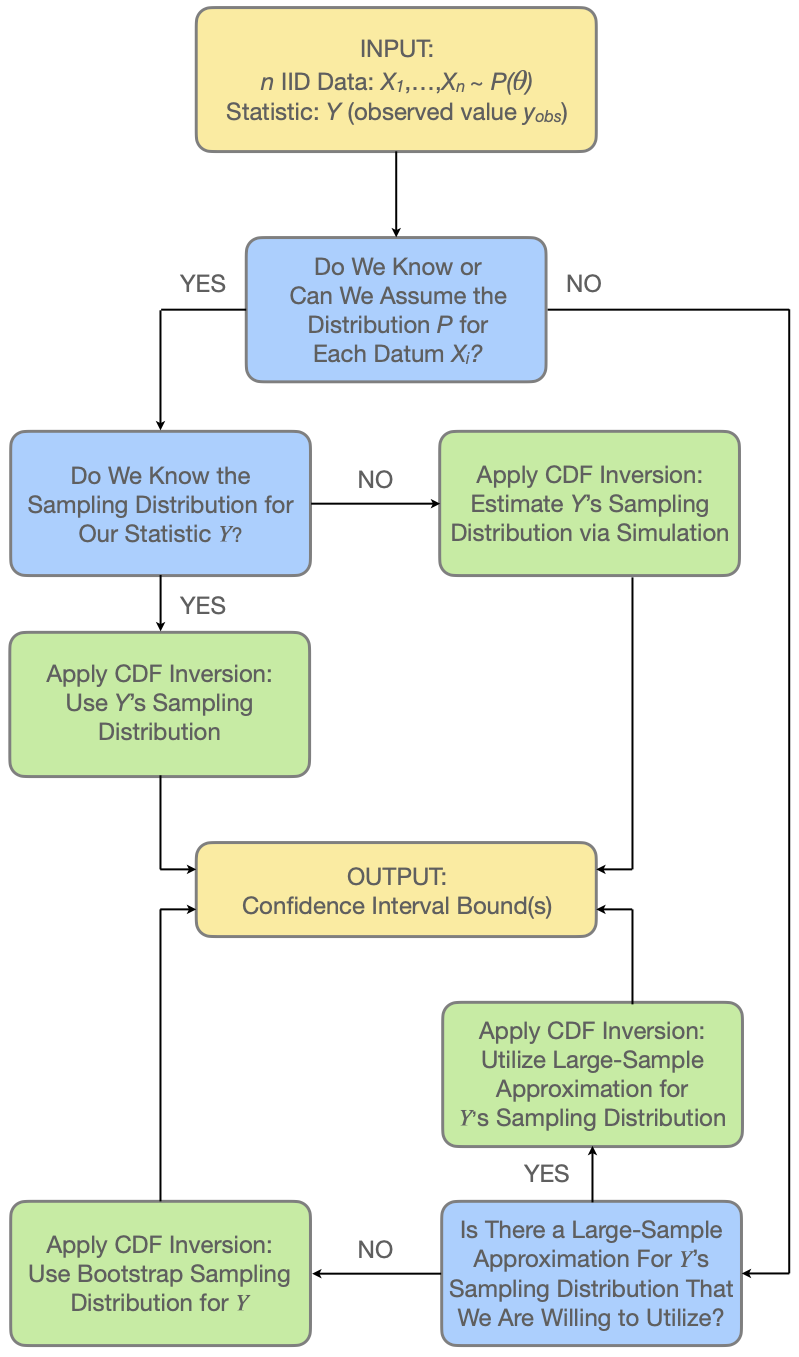
\includegraphics[width=0.625\linewidth,height=\textheight,keepaspectratio]{figures/ci_flowchart.png}

}

\caption{\label{fig-ciflowchart}A flowchart showing how to apply our
confidence interval methodology (dubbed cdf inversion in the chart) in
different analysis situations. From Freeman (2026).}

\end{figure}%

For more on confidence intervals, go to
Section~\ref{sec-chap5confidence}.

\subsection{Examples}\label{examples-41}

\subsubsection{Poisson Expected Counts: Confidence
Interval}\label{poisson-expected-counts-confidence-interval}

\begin{quote}
Assume that we sample \(n\) iid data. We know that the sum
\(Y = \sum_{i=1}^n X_i\) is a sufficient statistic for \(\lambda\) and
that \(Y \sim\) Poisson(\(n\lambda\)). For this statistic,
\(E[Y] = n\lambda\), which increases with \(\lambda\), so we know that
we will utilize the ``yes'' lines of the confidence interval reference
table. Our observed test statistic is
\(y_{\mathrm{obs}} = \sum_{i=1}^n x_i\).
\end{quote}

\begin{Shaded}
\begin{Highlighting}[]
\CommentTok{\# Let\textquotesingle{}s assume we observe ten years of data in a Poisson process}
\FunctionTok{set.seed}\NormalTok{(}\DecValTok{101}\NormalTok{)}
\NormalTok{alpha  }\OtherTok{\textless{}{-}} \FloatTok{0.05}
\NormalTok{n      }\OtherTok{\textless{}{-}} \DecValTok{10}
\NormalTok{lambda }\OtherTok{\textless{}{-}} \DecValTok{8}
\NormalTok{X      }\OtherTok{\textless{}{-}} \FunctionTok{rpois}\NormalTok{(n, }\AttributeTok{lambda =}\NormalTok{ lambda)}

\NormalTok{f }\OtherTok{\textless{}{-}} \ControlFlowTok{function}\NormalTok{(nlambda, y.obs, q)}
\NormalTok{\{}
  \FunctionTok{ppois}\NormalTok{(y.obs, }\AttributeTok{lambda =}\NormalTok{ nlambda) }\SpecialCharTok{{-}}\NormalTok{ q}
\NormalTok{\}}

\FunctionTok{round}\NormalTok{(}\FunctionTok{uniroot}\NormalTok{(f, }\AttributeTok{interval =} \FunctionTok{c}\NormalTok{(}\FloatTok{0.001}\NormalTok{, }\DecValTok{10000}\NormalTok{), }\AttributeTok{y.obs =} \FunctionTok{sum}\NormalTok{(X) }\SpecialCharTok{{-}} \DecValTok{1}\NormalTok{,}
              \AttributeTok{q =} \DecValTok{1} \SpecialCharTok{{-}}\NormalTok{ alpha }\SpecialCharTok{/} \DecValTok{2}\NormalTok{)}\SpecialCharTok{$}\NormalTok{root }\SpecialCharTok{/}\NormalTok{ n, }\DecValTok{3}\NormalTok{)}
\end{Highlighting}
\end{Shaded}

\begin{verbatim}
[1] 5.722
\end{verbatim}

\begin{Shaded}
\begin{Highlighting}[]
\FunctionTok{round}\NormalTok{(}\FunctionTok{uniroot}\NormalTok{(f, }\AttributeTok{interval =} \FunctionTok{c}\NormalTok{(}\FloatTok{0.001}\NormalTok{, }\DecValTok{10000}\NormalTok{), }\AttributeTok{y.obs =} \FunctionTok{sum}\NormalTok{(X),}
              \AttributeTok{q =}\NormalTok{     alpha }\SpecialCharTok{/} \DecValTok{2}\NormalTok{)}\SpecialCharTok{$}\NormalTok{root }\SpecialCharTok{/}\NormalTok{ n, }\DecValTok{3}\NormalTok{)}
\end{Highlighting}
\end{Shaded}

\begin{verbatim}
[1] 9.179
\end{verbatim}

\begin{quote}
Note both the discreteness correction that we apply when deriving the
lower bound and the division by \(n\) after the calls to
\texttt{uniroot()}. The latter converts the interval bounds from being
ones on \(n\lambda\) to being ones on \(\lambda\) itself. The interval
is \([\hat{\lambda}_L,\hat{\lambda}_U] =
[5.72,9.18]\), which overlaps the true value of 8. (See
Figure~\ref{fig-poici}.) Note that the interval over which we search for
the root is {[}0.001,10000{]}, which is (effectively) the range of
possible values for \(\lambda\). (Recall that \(\lambda > 0\), hence the
small but non-zero lower bound for \texttt{interval}.)
\end{quote}

\begin{figure}

\begin{minipage}[t]{0.50\linewidth}

\centering{

\pandocbounded{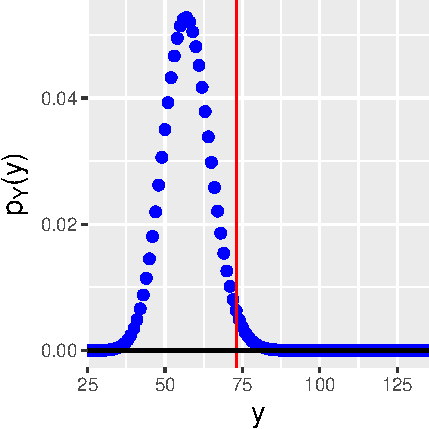
\includegraphics[keepaspectratio]{04-poisson_files/figure-latex/fig-poici-1.pdf}}

}

\subcaption{\label{fig-poici-1}}

\end{minipage}%
%
\begin{minipage}[t]{0.50\linewidth}

\centering{

\pandocbounded{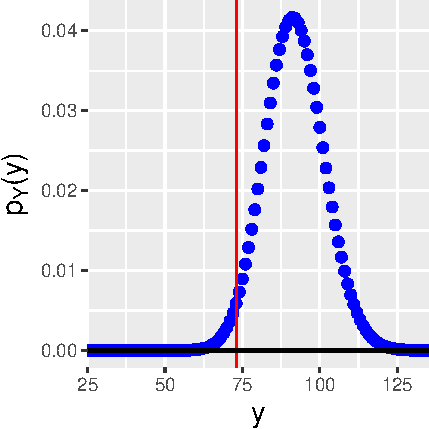
\includegraphics[keepaspectratio]{04-poisson_files/figure-latex/fig-poici-2.pdf}}

}

\subcaption{\label{fig-poici-2}}

\end{minipage}%

\caption{\label{fig-poici}Probability mass functions for Poisson
distributions for which (a) \(n\lambda=57.2\), and (b)
\(n\lambda=91.8\). We assume that we observe
\(y_{\mathrm{obs}} = \sum_{i=1}^n x_i = 73\) events in total and that we
want to construct a 95\% confidence interval for \(\lambda\).
\(n\lambda=57.2\) is the smallest value of \(n\lambda\) such that
\(F_Y^{-1}(0.975) = 73\), while \(n\lambda=91.8\) is the largest value
of \(n\lambda\) such that \(F_Y^{-1}(0.025) = 73\).}

\end{figure}%

\begin{quote}
In Section~\ref{sec-chap3confidence}, we discussed how when we work with
discrete sampling distributions, the coverage of the confidence
intervals that we construct, given a value \(\theta = \theta_o\), will
be equal to the probability of sampling a datum in the acceptance region
given a null hypothesis \(H_o : \theta = \theta_o\), and thus the
coverage will be, in general, \(> 1-\alpha\). Let's verify that that is
the case here.
\end{quote}

\begin{Shaded}
\begin{Highlighting}[]
\CommentTok{\# here, lambda = 8}
\NormalTok{y.rr.lo }\OtherTok{\textless{}{-}} \FunctionTok{qpois}\NormalTok{(    alpha }\SpecialCharTok{/} \DecValTok{2}\NormalTok{, }\AttributeTok{lambda =}\NormalTok{ lambda)}
\NormalTok{y.rr.hi }\OtherTok{\textless{}{-}} \FunctionTok{qpois}\NormalTok{(}\DecValTok{1} \SpecialCharTok{{-}}\NormalTok{ alpha }\SpecialCharTok{/} \DecValTok{2}\NormalTok{, }\AttributeTok{lambda =}\NormalTok{ lambda)}
\FunctionTok{round}\NormalTok{(}\FunctionTok{sum}\NormalTok{(}\FunctionTok{dpois}\NormalTok{(y.rr.lo}\SpecialCharTok{:}\NormalTok{y.rr.hi, }\AttributeTok{lambda =}\NormalTok{ lambda)), }\DecValTok{3}\NormalTok{)}
\end{Highlighting}
\end{Shaded}

\begin{verbatim}
[1] 0.969
\end{verbatim}

\begin{quote}
If \(\lambda = 8\), the coverage of our interval estimates is 96.9\%.
\end{quote}

\subsubsection{Death-by-Horse-Kick: Confidence
Interval}\label{death-by-horse-kick-confidence-interval}

\begin{quote}
Previously, we determined that a point estimate for the expected number
of deaths from horse kicks in any one Prussian army corps during any one
year is \(\hat{\lambda} = 0.61\). Here, we determine a 95\% two-sided
interval estimate for \(\lambda\).
\end{quote}

\begin{Shaded}
\begin{Highlighting}[]
\NormalTok{X     }\OtherTok{\textless{}{-}} \FunctionTok{c}\NormalTok{(}\FunctionTok{rep}\NormalTok{(}\DecValTok{0}\NormalTok{, }\DecValTok{109}\NormalTok{), }\FunctionTok{rep}\NormalTok{(}\DecValTok{1}\NormalTok{, }\DecValTok{65}\NormalTok{), }\FunctionTok{rep}\NormalTok{(}\DecValTok{2}\NormalTok{, }\DecValTok{22}\NormalTok{), }\FunctionTok{rep}\NormalTok{(}\DecValTok{3}\NormalTok{, }\DecValTok{3}\NormalTok{), }\FunctionTok{rep}\NormalTok{(}\DecValTok{4}\NormalTok{, }\DecValTok{1}\NormalTok{))}
\NormalTok{n     }\OtherTok{\textless{}{-}} \FunctionTok{length}\NormalTok{(X)}
\NormalTok{alpha }\OtherTok{\textless{}{-}} \FloatTok{0.05}

\NormalTok{f }\OtherTok{\textless{}{-}} \ControlFlowTok{function}\NormalTok{(nlambda, y.obs, q)}
\NormalTok{\{}
  \FunctionTok{ppois}\NormalTok{(y.obs, }\AttributeTok{lambda =}\NormalTok{ nlambda) }\SpecialCharTok{{-}}\NormalTok{ q}
\NormalTok{\}}

\FunctionTok{round}\NormalTok{(}\FunctionTok{uniroot}\NormalTok{(f, }\AttributeTok{interval =} \FunctionTok{c}\NormalTok{(}\FloatTok{0.001}\NormalTok{, }\DecValTok{10000}\NormalTok{), }\AttributeTok{y.obs =} \FunctionTok{sum}\NormalTok{(X) }\SpecialCharTok{{-}} \DecValTok{1}\NormalTok{,}
              \AttributeTok{q =} \DecValTok{1} \SpecialCharTok{{-}}\NormalTok{ alpha }\SpecialCharTok{/} \DecValTok{2}\NormalTok{)}\SpecialCharTok{$}\NormalTok{root }\SpecialCharTok{/}\NormalTok{ n, }\DecValTok{3}\NormalTok{)}
\end{Highlighting}
\end{Shaded}

\begin{verbatim}
[1] 0.507
\end{verbatim}

\begin{Shaded}
\begin{Highlighting}[]
\FunctionTok{round}\NormalTok{(}\FunctionTok{uniroot}\NormalTok{(f, }\AttributeTok{interval =} \FunctionTok{c}\NormalTok{(}\FloatTok{0.001}\NormalTok{, }\DecValTok{10000}\NormalTok{), }\AttributeTok{y.obs =} \FunctionTok{sum}\NormalTok{(X),}
              \AttributeTok{q =}\NormalTok{     alpha }\SpecialCharTok{/} \DecValTok{2}\NormalTok{)}\SpecialCharTok{$}\NormalTok{root }\SpecialCharTok{/}\NormalTok{ n, }\DecValTok{3}\NormalTok{)}
\end{Highlighting}
\end{Shaded}

\begin{verbatim}
[1] 0.728
\end{verbatim}

\begin{quote}
The 95\% confidence interval is \([0.507,0.728]\).
\end{quote}

\subsubsection{Death-by-Horse-Kick: Nonparametric Bootstrap Confidence
Interval}\label{death-by-horse-kick-nonparametric-bootstrap-confidence-interval}

\begin{quote}
The bootstrap, introduced in Efron (1979), uses the observed data
themselves to build up empirical sampling distributions for statistics.
(Note that here we are specifically referring to the \emph{nonparametric
bootstrap} procedure. Other bootstrap procedures exist; see, e.g.,
Hesterberg (2015) and references therein.) Let's suppose we are handed
the following data: \[
\mathbf{X} = \{X_1,X_2,\ldots,X_n\} \overset{iid}{\sim} P \,,
\] where the distribution \(P\) is unknown. Now, let's suppose further
that from these data we compute a statistic: a single number. How can we
build up an empirical sampling distribution from a single number? The
answer is to repeatedly \emph{resample} the data we observe, \emph{with
replacement}. For instance, if we have as data the numbers
\(\{1,2,3\}\), a bootstrap sample might be \(\{1,1,3\}\) or
\(\{2,3,3\}\), etc. Every time we resample the data, we compute the
statistic we are interested in and record its value. Voila: we have an
empirical sampling distribution. And if we can link the elements of that
sampling distribution to a population parameter, we can immediately
write down a confidence interval. For instance, if we have the
\(n_{\mathrm{boot}}\) statistics \(\{\bar{X}_1,\ldots,\bar{X}_k\}\), we
can put bounds on the population mean \(\mu\): \begin{align*}
\hat{\mu}_L &= \bar{X}_{\alpha/2} \\
\hat{\mu}_U &= \bar{X}_{1-\alpha/2} \,,
\end{align*} where \(\alpha/2\) and \(1-\alpha/2\) represent sample
percentiles, e.g., the 2.5\(^{\mathrm{th}}\) and 97.5\(^{\mathrm{th}}\)
percentiles.
\end{quote}

\begin{quote}
What is a 95\% two-sided bootstrap confidence interval on the expected
number of deaths by horse kick per Prussian army corps per year?
\end{quote}

\begin{Shaded}
\begin{Highlighting}[]
\CommentTok{\# We are utilizing the same variable X defined above}
\NormalTok{n.boot }\OtherTok{\textless{}{-}} \DecValTok{10000}
\NormalTok{x.bar  }\OtherTok{\textless{}{-}} \FunctionTok{rep}\NormalTok{(}\ConstantTok{NA}\NormalTok{, n.boot)}
\ControlFlowTok{for}\NormalTok{ ( ii }\ControlFlowTok{in} \DecValTok{1}\SpecialCharTok{:}\NormalTok{n.boot ) \{}
\NormalTok{  s         }\OtherTok{\textless{}{-}} \FunctionTok{sample}\NormalTok{(}\FunctionTok{length}\NormalTok{(X), }\FunctionTok{length}\NormalTok{(X), }\AttributeTok{replace =} \ConstantTok{TRUE}\NormalTok{)}
\NormalTok{  x.bar[ii] }\OtherTok{\textless{}{-}} \FunctionTok{mean}\NormalTok{(X[s])}
\NormalTok{\}}
\FunctionTok{round}\NormalTok{(}\FunctionTok{quantile}\NormalTok{(x.bar, }\AttributeTok{probs =} \FunctionTok{c}\NormalTok{(}\FloatTok{0.025}\NormalTok{, }\FloatTok{0.975}\NormalTok{)), }\DecValTok{3}\NormalTok{)}
\end{Highlighting}
\end{Shaded}

\begin{verbatim}
 2.5% 97.5% 
0.505 0.720 
\end{verbatim}

\begin{quote}
The estimated interval is \([0.505,0.725]\). This is on par with what we
observe above, but we will note that in general the nonparametric
bootstrap procedure suffers from what Hesterberg (2015) dubs a
``narrowness bias'': the coverage of its intervals is smaller than
\(1-\alpha/2\) for small samples, converging to \(1-\alpha/2\) as
\(n \rightarrow \infty\). (We have \(n = 200\) data here, so the
narrowness bias is effectively moot.) When we can propose a plausible
distribution for our data, we should do so, as we will generate more
meaningful confidence intervals (even if simulations are involved) than
if we lazily fall back upon bootstrapping.
\end{quote}

\subsubsection{Bootstrap Sample: Proportion of Observed
Data}\label{bootstrap-sample-proportion-of-observed-data}

\begin{quote}
Let's assume that we sample \(n\) iid data from some distribution \(P\).
When we create a bootstrap sample of these data, some of the observed
data appear multiple times, while other data do not appear at all. What
is the average proportion of observed data in any given bootstrap
sample?
\end{quote}

\begin{quote}
Let \(i\) be the index of an arbitrary datum, where the indices are
\(\{1,2,\ldots,n-1,n\}\). Let \(X\) be the number of times \(i\) is
chosen when we construct a bootstrap sample of size \(n\). We can see
immediately that data sampling is a series of Bernoulli trials (i.e.,
either we pick a particular datum, with probability \(1/n\), or we do
not), so \(X \sim\) Binom(\(n, 1/n\)). The probability of observing a
particular datum one or more times, \(P(X \geq 1)\), then represents the
average proportion of observed data in a bootstrap sample: \[
P(X \geq 1) = 1 - P(X = 0) = 1 - (1-1/n)^n \,,
\] which, as \(n \rightarrow \infty\), approaches \(1-1/e = 0.632\).
Thus, for a sufficiently large sample, 63.2\% of the observed data will
appear at least once in a bootstrapped dataset.
\end{quote}

\subsubsection{Death-by-Horse Kick: Simulation-Based Confidence
Interval}\label{death-by-horse-kick-simulation-based-confidence-interval}

\begin{quote}
Let's assume that we do not know that the sampling distribution for the
sum of \(n\) iid Poisson random variables is Poisson(\(n\lambda\)), but
that we can assume each datum \emph{is itself} sampled according to a
Poisson distribution. To determine a confidence interval for
\(\lambda\), then, we can utilize numerical simulations, to estimate
empirical sampling distributions for \(Y\) given candidate values of
\(\lambda\), and determining those values of \(\lambda\) that make
\(F_Y(y_{\mathrm{obs}} \vert \lambda)\) (at least approximately) equal
to 0.025 and 0.975.
\end{quote}

\begin{quote}
Let's first build up the code that we would need to construct the
empirical cumulative distribution function:
\end{quote}

\begin{verbatim}
X <- matrix(rpois(n*num.sim, lambda=lambda), nrow=num.sim)
Y <- apply(X, 1, function(x){sum(x)})  # we still know the sum is sufficient
sum(Y <= y.obs)/num.sim
\end{verbatim}

\begin{quote}
On the first line, we create \texttt{num.sim} separate datasets given a
parameter value, and store them row-by-row in a matrix. On the second
line, we use \texttt{R}'s \texttt{apply()} function, row-by-row (as
indicated by the argument \texttt{1}), to determine the statistic value
for each dataset. Then, on the third line, we determine the proportion
of statistic values that are less than or equal to \(y_{\mathrm{obs}}\):
this is the empirical cumulative distribution function value
\(\hat{F}_n(y_{\mathrm{obs}} \vert a)\). We then find the value of \(a\)
for which \(\hat{F}_n(y_{\mathrm{obs}} \vert a) - q = 0\) using
\texttt{uniroot()}.
\end{quote}

\begin{quote}
Let's put this all together in an example where \(n = 5\) and
\(y_{\mathrm{obs}} = 10\):
\end{quote}

\begin{Shaded}
\begin{Highlighting}[]
\CommentTok{\# We utilize the same data vector X defined above}
\NormalTok{n     }\OtherTok{\textless{}{-}} \FunctionTok{length}\NormalTok{(X)}
\NormalTok{y.obs }\OtherTok{\textless{}{-}} \FunctionTok{sum}\NormalTok{(X)}
\NormalTok{alpha }\OtherTok{\textless{}{-}} \FloatTok{0.05}

\CommentTok{\# Note: we are generating data with lambda, so the CI is for lambda, not n*lambda}
\NormalTok{f }\OtherTok{\textless{}{-}} \ControlFlowTok{function}\NormalTok{(lambda, n, y.obs, q, }\AttributeTok{num.sim =} \DecValTok{1000000}\NormalTok{, }\AttributeTok{seed =} \DecValTok{236}\NormalTok{)}
\NormalTok{\{}
  \FunctionTok{set.seed}\NormalTok{(seed)}
\NormalTok{  X }\OtherTok{\textless{}{-}} \FunctionTok{matrix}\NormalTok{(}\FunctionTok{rpois}\NormalTok{(n }\SpecialCharTok{*}\NormalTok{ num.sim, }\AttributeTok{lambda =}\NormalTok{ lambda), }\AttributeTok{nrow =}\NormalTok{ num.sim)}
\NormalTok{  Y }\OtherTok{\textless{}{-}} \FunctionTok{rowSums}\NormalTok{(X)  }\CommentTok{\# equivalent to apply(X, 1, function(x)\{sum(x)\})}
  \FunctionTok{sum}\NormalTok{(Y }\SpecialCharTok{\textless{}=}\NormalTok{ y.obs) }\SpecialCharTok{/}\NormalTok{ num.sim }\SpecialCharTok{{-}}\NormalTok{ q}
\NormalTok{\}}

\FunctionTok{round}\NormalTok{(}\FunctionTok{uniroot}\NormalTok{(f, }\AttributeTok{interval =} \FunctionTok{c}\NormalTok{(}\FloatTok{0.001}\NormalTok{, }\DecValTok{1000}\NormalTok{), }\AttributeTok{n =}\NormalTok{ n, }\AttributeTok{y.obs =}\NormalTok{ y.obs }\SpecialCharTok{{-}} \DecValTok{1}\NormalTok{, }
              \AttributeTok{q =} \DecValTok{1} \SpecialCharTok{{-}}\NormalTok{ alpha }\SpecialCharTok{/} \DecValTok{2}\NormalTok{, }\AttributeTok{num.sim =} \DecValTok{100000}\NormalTok{)}\SpecialCharTok{$}\NormalTok{root, }\DecValTok{3}\NormalTok{)}
\end{Highlighting}
\end{Shaded}

\begin{verbatim}
[1] 0.507
\end{verbatim}

\begin{Shaded}
\begin{Highlighting}[]
\FunctionTok{round}\NormalTok{(}\FunctionTok{uniroot}\NormalTok{(f, }\AttributeTok{interval =} \FunctionTok{c}\NormalTok{(}\FloatTok{0.001}\NormalTok{, }\DecValTok{1000}\NormalTok{), }\AttributeTok{n =}\NormalTok{ n, }\AttributeTok{y.obs =}\NormalTok{ y.obs    ,}
              \AttributeTok{q =}\NormalTok{     alpha }\SpecialCharTok{/} \DecValTok{2}\NormalTok{, }\AttributeTok{num.sim =} \DecValTok{100000}\NormalTok{)}\SpecialCharTok{$}\NormalTok{root, }\DecValTok{3}\NormalTok{)}
\end{Highlighting}
\end{Shaded}

\begin{verbatim}
[1] 0.728
\end{verbatim}

\begin{quote}
Our simulation-based 95\% confidence interval for \(\lambda\) is
{[}0.507,0.728{]}, which is equivalent to the one determined using the
fact that the sum of the data are Poisson-distributed with parameter
\(n\lambda\). To be clear: simulation-based confidence intervals are
\textbf{exact} to within machine tolerance (the fact that
\texttt{sum(Y\ \textless{}=\ y.obs)\ /\ num.sim} and \texttt{q} can
differ by \(\sim 10^{-4}\) by default) and any uncertainty in the value
of the empirical cdf \(\hat{F}_n(y_{\mathrm{obs}} \vert \lambda)\) due
to our use of a finite number of simulated datasets, \texttt{num.sim}.
Regarding the second point: the empirical cdf is an \emph{estimate},
i.e., even if we hold \(\lambda\) constant,
\texttt{sum(Y\ \textless{}=\ y.obs)} is a random variable whose value
can change as we change the random number generator seed value. Let's
denote the sum as \(S \vert \lambda\), the total number of simulated
datasets as \(k\), and the true cdf value (given \(y_{\mathrm{obs}}\))
as \(p\). Then \begin{align*}
S \vert \lambda \sim \text{Binomial}(k, p) \,.
\end{align*} The standard error for the empirical cdf is thus
\begin{align*}
\sqrt{V\left[\frac{1}{k}(S \vert \lambda)\right]} = \sqrt{\frac{p(1-p)}{k}} \,.
\end{align*} If \(k = 10^5\) and, e.g., \(p = 0.025\), the standard
error is \(\sim 10^{-4}\). Combining this value with the tolerance of
\texttt{uniroot()}, we expect the uncertainties of our interval bound
estimates to be \(\sim 10^{-4}\). (Particularly if we utilize a larger
number of simulated datasets. Above, we set \texttt{num.sim} to a
smaller value because, ultimately, we multiply this value by \(n\), and
since \(n = 200\), we need to be mindful to not utilize too much
computer memory and to not make the computation time too long. Each
\texttt{uniroot()} call in the code given here generates results in
\(\lesssim\) 10 CPU seconds on a standard desktop or laptop computer.)
\end{quote}

\subsubsection{Zero-Truncated Poisson Expected Counts: Simulation-Based
Confidence
Interval}\label{zero-truncated-poisson-expected-counts-simulation-based-confidence-interval}

\begin{quote}
In Section~\ref{sec-chap4linear}, we derived the moment-generating
function for the zero-inflated Poisson distribution and wrote down the
mgf for the zero-truncated Poisson distribution, and indicated that we
could use neither of them to determine the sampling distribution of,
e.g., the sample sum given \(n\) iid random variables. As indicated in
Figure~\ref{fig-ciflowchart}, when we do not know the sampling
distribution of \(Y\), but we do know the distribution for each
individual datum, we can utilize simulations to derive exact confidence
intervals. We will demonstrate that here for the zero-truncated
distribution.
\end{quote}

\begin{quote}
Let's assume that we conduct an experiment in which we gather the
following data:
\end{quote}

\begin{Shaded}
\begin{Highlighting}[]
\FunctionTok{suppressMessages}\NormalTok{(}\FunctionTok{library}\NormalTok{(actuar))}
\end{Highlighting}
\end{Shaded}

\begin{verbatim}
Warning: package 'actuar' was built under R version 4.5.2
\end{verbatim}

\begin{Shaded}
\begin{Highlighting}[]
\FunctionTok{set.seed}\NormalTok{(}\DecValTok{236}\NormalTok{)}
\NormalTok{n      }\OtherTok{\textless{}{-}} \DecValTok{10}
\NormalTok{lambda }\OtherTok{\textless{}{-}} \DecValTok{3}
\NormalTok{(X     }\OtherTok{\textless{}{-}} \FunctionTok{rztpois}\NormalTok{(n, lambda))}
\end{Highlighting}
\end{Shaded}

\begin{verbatim}
 [1] 2 4 2 3 2 3 5 3 3 1
\end{verbatim}

\begin{quote}
We decide that we wish to construct a 95\% lower bound on \(\lambda\).
The reader can verify that a sufficient statistic for \(\lambda\) is
\(Y = \sum_{i=1}^n X_i\), and that \(E[Y]\) increases with \(\lambda\)
(meaning that \(q = 1-\alpha = 0.95\)). Given this information and the
simulation framework laid out in the last example, determining the lower
bound is straightforward:
\end{quote}

\begin{Shaded}
\begin{Highlighting}[]
\NormalTok{n     }\OtherTok{\textless{}{-}} \FunctionTok{length}\NormalTok{(X)}
\NormalTok{y.obs }\OtherTok{\textless{}{-}} \FunctionTok{sum}\NormalTok{(X)}
\NormalTok{alpha }\OtherTok{\textless{}{-}} \FloatTok{0.05}

\NormalTok{f }\OtherTok{\textless{}{-}} \ControlFlowTok{function}\NormalTok{(lambda, n, y.obs, q, }\AttributeTok{num.sim =} \DecValTok{1000000}\NormalTok{, }\AttributeTok{seed =} \DecValTok{236}\NormalTok{)}
\NormalTok{\{}
  \FunctionTok{set.seed}\NormalTok{(seed)}
\NormalTok{  X }\OtherTok{\textless{}{-}} \FunctionTok{matrix}\NormalTok{(}\FunctionTok{rztpois}\NormalTok{(n }\SpecialCharTok{*}\NormalTok{ num.sim, }\AttributeTok{lambda =}\NormalTok{ lambda), }\AttributeTok{nrow =}\NormalTok{ num.sim)}
\NormalTok{  Y }\OtherTok{\textless{}{-}} \FunctionTok{rowSums}\NormalTok{(X)  }\CommentTok{\# equivalent to apply(X, 1, function(x)\{sum(x)\})}
  \FunctionTok{sum}\NormalTok{(Y }\SpecialCharTok{\textless{}=}\NormalTok{ y.obs) }\SpecialCharTok{/}\NormalTok{ num.sim }\SpecialCharTok{{-}}\NormalTok{ q}
\NormalTok{\}}

\FunctionTok{round}\NormalTok{(}\FunctionTok{uniroot}\NormalTok{(f, }\AttributeTok{interval =} \FunctionTok{c}\NormalTok{(}\FloatTok{0.001}\NormalTok{, }\DecValTok{1000}\NormalTok{), }\AttributeTok{n =}\NormalTok{ n, }\AttributeTok{y.obs =}\NormalTok{ y.obs,}
              \AttributeTok{q =} \DecValTok{1} \SpecialCharTok{{-}}\NormalTok{ alpha)}\SpecialCharTok{$}\NormalTok{root, }\DecValTok{3}\NormalTok{)}
\end{Highlighting}
\end{Shaded}

\begin{verbatim}
[1] 1.848
\end{verbatim}

\begin{quote}
The 95\% lower bound on \(\lambda\) is 1.848.
\end{quote}

\section{Hypothesis Testing: Likelihood Ratio
Test}\label{sec-chap4hypothesis}

What to take away from this section:

\begin{itemize}
\item
  While the \emph{Neyman-Pearson lemma} states that a ratio of
  likelihood functions constitutes \textbf{the most powerful test} of
  the simple hypotheses \(H_o : \theta = \theta_o\) and
  \(H_a : \theta = \theta_a\), we cannot extend that result to state a
  most powerful test of composite hypotheses.
\item
  A commonly used test of composite hypothesis is the \emph{likelihood
  ratio test}, or \emph{LRT}.
\item
  If we are working with a member of the exponential family of
  distributions, then to carry out the LRT, we should simply conduct a
  hypothesis test in the manner described in
  Section~\ref{sec-chap1hypothesis} and
  Section~\ref{sec-chap2hypothesis} while utilizing a \emph{sufficient
  statistic} for \(\theta\).
\item
  Given a single vector of Poisson data \(\{X_1,\ldots,X_m\}\), where
  \(\sum_{i=1}^m X_i = k\), and a null hypothesis that the expected data
  proportions across the bins are \(\{p_{1,o},\ldots,p_{m,o}\}\), we can
  carry out a set of \(m\) separate Poisson-based hypothesis tests and
  aggregate the \(m\) \(p\)-values into a single \(p\)-value.
\end{itemize}

For previous material on hypothesis testing, see
Section~\ref{sec-chap3nplemma} and Section~\ref{sec-chap3categorical}.

\smallskip\hrule

\begin{quote}
\textbf{Recall}: \emph{a hypothesis test is a framework to make an
inference about the value of a population parameter \(\theta\). The null
hypothesis \(H_o\) is that \(\theta = \theta_o\), while possible
alternatives \(H_a\) are \(\theta \neq \theta_o\) (two-tail test),
\(\theta > \theta_o\) (upper-tail test), and \(\theta < \theta_o\)
(lower-tail test). For, e.g., a one-tail test, we reject the null
hypothesis if the observed test statistic \(y_{\mathrm{obs}}\) falls
outside the bound given by \(y_{RR}\), which is a solution to the
equation} \[
F_Y(y_{RR} \vert \theta_o) - q = 0 \,,
\] \emph{where \(F_Y(\cdot)\) is the cumulative distribution function
for the statistic \(Y\) and \(q\) is an appropriate quantile value that
is a function of the adopted Type I error rate \(\alpha\). Note that the
hypothesis test framework only allows us to make a decision about a null
hypothesis; nothing is proven.}
\end{quote}

\smallskip\hrule

In Section~\ref{sec-chap3nplemma}, we built upon the framework described
above by introducing the Neyman-Pearson lemma. This result allows us to
bypass the ``guesswork'' that goes into selecting a hypothesis test
statistic, by defining the most powerful test of a simple null
hypothesis versus a simple specified alternative.

\smallskip\hrule

\begin{quote}
\textbf{Recall:} \emph{when we test the simple hypotheses
\(H_o: \theta = \theta_o\) versus \(H_a: \theta = \theta_a\), the
Neyman-Pearson lemma allows us to state that the hypothesis test with
maximum power has a rejection region of the form} \[
\frac{\mathcal{L}(\theta_o \vert \mathbf{x})}{\mathcal{L}(\theta_a \vert \mathbf{x})} < c(\alpha) \,,
\] \emph{where \(c(\alpha)\) is a constant whose value depends on the
specified Type I error \(\alpha\). When we sample data from an
exponential-family distribution, we would simply determine a sufficient
statistic \(Y\), and develop a hypothesis test as we have done
previously using that statistic (or a function of it), assuming we know
or can assume its sampling distribution. If the rejection region does
not depend on \(\theta_a\), then the test is said to be a uniformly most
powerful (UMP) test.}
\end{quote}

\smallskip\hrule

In an example, we demonstrate how to apply the NP lemma to construct a
hypothesis test for the Poisson parameter \(\lambda\), given a sample of
\(n\) iid data.

Here we will build on our discussion of the Neyman-Pearson lemma and
describe a more general hypothesis test framework, one dubbed the
\emph{likelihood ratio test} (or \emph{LRT}).

``Wait\ldots the NP lemma had a likelihood ratio. How is the LRT
different?''

That is a good question. It differs in how we specify the null and
alternative hypotheses: \[
H_o: \theta \in \Theta_o ~~\mbox{vs.}~~ H_a: \theta \in \Theta_o^c \,,
\] where \(\Theta_o\) (``capital theta naught'') represents a set of
possible null values for \(\theta\), while \(\Theta_o^c\) is the
complement of that set. For instance, for tests involving the Poisson
parameter \(\lambda\), \(\Theta_o\) could be \(\lambda \in [5,10]\), so
that \(\Theta_o^c\) is \(\lambda < 5\) or \(\lambda > 10\). (Thus the
null and alternative hypotheses can both be composite hypotheses, as
opposed to simple ones.) Let \(\Theta = \Theta_o \cup \Theta_o^c\),
i.e., the union of the null and alternative sets. The rejection region
for the LRT is \[
\lambda_{LR} = \frac{\mbox{sup}_{\theta \in \Theta_o} \mathcal{L}(\theta \vert \mathbf{x})}{\mbox{sup}_{\theta \in \Theta} \mathcal{L}(\theta \vert \mathbf{x})} < c(\alpha) \,,
\] where, like it is in the context of the NP lemma, \(c(\alpha)\) is a
constant that depends on the specified Type I error \(\alpha\).

``Since the LRT is more general, why would we ever utilize the NP
lemma?''

That is another good question.

The primary point to make is that when we construct a test of two simple
hypothesis within the framework of the NP lemma, we \emph{know} that we
are constructing the most powerful test of those hypotheses. On the
other hand, while the LRT is generally a powerful test, given the
composite nature of one (or both) of the hypotheses it comes with no
guarantee of being the most powerful test. For instance, perhaps an
alternative like the score test (also known as the Lagrange multiplier
test) or the Wald test would provide the most powerful test in a given
analysis situation, although one should keep in mind that it is usually
the case that the power of these tests are effectively identical. A
reader who is interested in learning more about them should look at
section 10.3 of Casella and Berger (2002) and at Buse (1982), while
noting that the latter implicitly describes two-tail tests only.

How does using the likelihood ratio test play out in practice? Let's
look at some possible use cases. For simplicity, below we will assume
that we have sampled data from an exponential-family distribution, and
thus that we can reduce the data to, e.g., a single-number sufficient
statistic for \(\theta\). If we were to sample data according to a
non-exponential-family distribution, we could, as we did in
Section~\ref{sec-chap3nplemma}, fall back upon the use of simulations to
determine the empirical distribution of the statistic \(\lambda_{LR}\)
(or \(\log\lambda_{LR}\)) under the null and use that distribution to
estimate, e.g., the \(p\)-value.

\begin{enumerate}
\def\labelenumi{\arabic{enumi}.}
\tightlist
\item
  We have one freely varying parameter \(\theta\) and we wish to test
  \(H_o : \theta = \theta_o\) versus \(H_a : \theta \neq \theta_o\).
\end{enumerate}

In this situation, we identify a sufficient statistic (or a one-to-one
function of it) for which we know the sampling distribution and use it
to define a two-tail test as we have done previously, utilizing the
hypothesis test reference tables.

\begin{enumerate}
\def\labelenumi{\arabic{enumi}.}
\setcounter{enumi}{1}
\tightlist
\item
  We have one freely varying parameter \(\theta\) and we wish to define
  a one-sided alternative hypothesis, e.g., \(H_a : \theta < \theta_o\).
\end{enumerate}

Here, the null hypothesis would be the complement of \(H_a\), i.e.,
\(H_o : \theta \geq \theta_o\). The distribution of the ratio \[
\lambda_{LR} = \frac{\mbox{sup}_{\theta \geq \theta_o} \mathcal{L}(\theta \vert \mathbf{x})}{\mathcal{L}(\hat{\theta}_{MLE} \vert \mathbf{x})}
\] is thus not uniquely specifiable: it is a function of \(\theta\), and
our null does not state a specific value for \(\theta\). So how would we
determine \(y_{\mathrm{RR}}\)? It turns out the most conservative
rejection-region boundary we can specify, which would be the one that is
associated with the highest \(p\)-value we can observe, is the one that
we would derive assuming that \(\theta = \theta_o\)\ldots which means
that to define an LRT, we would simply assume \(\theta_o\) as our null
value, identify a sufficient statistic (or a one-to-one function of it)
for which we know the sampling distribution, and define a one-tail test
as we have done previously.

At this point, it is important to note that the way that we have defined
one-tail hypothesis tests previously (e.g., \(H_o : \theta = \theta_o\)
versus \(H_a : \theta < \theta_o\)) is the conventional way to define
them but not necessarily the correct way. A more precise definition of
the null would indicate that it is composite (e.g.,
\(H_o : \theta \geq \theta_o\)), but for the reason given above we would
still insert \(\theta_o\) itself into the \(p\)-value equation, etc. For
further discussion, see Jamshidian and Jamshidian (2026).

\begin{enumerate}
\def\labelenumi{\arabic{enumi}.}
\setcounter{enumi}{2}
\tightlist
\item
  We have two (or more) freely varying parameters, or alternatively, we
  have one freely varying parameter for a non-exponential-family
  distribution.
\end{enumerate}

In this context, we will have joint sufficient statistics that are
sampled according to a multivariate sampling distribution that will be
difficult, though not necessarily impossible, to work with directly. In
such a situation, we have historically fallen back on \emph{Wilks'
theorem}, although where possible we should utilize simulations like we
did in the context of the NP lemma (as we will demonstrate below).
(That's because Wilks' theorem utilizes the large-sample approximation
that the data are jointly distributed according to a multivariate normal
distribution. As this is only an approximation, simulations will yield
superior results in terms of precision and accuracy.)

Let \(r_o\) denote the number of free parameters in
\(H_o: \theta \in \Theta_o\) and let \(r\) denote the number of free
parameters in \(\theta \in \Theta = \Theta_o \cup \Theta_a\). (To
reiterate, \(\Theta\) must include \emph{all possible values of the
parameters}. For instance, if \(H_o\) is \(\theta = \theta_o\), then
\(H_a\) must be \(\theta \neq
\theta_o\) and not \(\theta < \theta_o\) or \(\theta > \theta_o\).) For
large \(n\), \[
-2\log \lambda_{LR} \overset{d}{\rightarrow} W \sim \chi_{r-r_o}^2 \,,
\] and we would reject the null hypothesis if
\(-2\log \lambda_{LR} > w_{\mathrm{RR}} = F_{W(r-r_o)}^{-1}(1-\alpha)\).
Since this result is related to the Central Limit Theorem, large \(n\)
would be, by rule-of-thumb, 30 or more.

For more on hypothesis testing, go to Section~\ref{sec-chap5hypothesis}.

\subsection{Examples}\label{examples-42}

\subsubsection{Poisson Expected Counts: Uniformly Most Powerful
Test}\label{poisson-expected-counts-uniformly-most-powerful-test}

\begin{quote}
Let's say that we are counting the number of students that enter a
classroom each minute. We assume that the entry of students is a
homogeneous Poisson process (i.e., \(\lambda\), the expected number of
entering students per time period, is constant). We think that five
students, on average, will pass through the door each minute, while
someone else thinks the number will be three. We collect data during
five independent one-minute intervals: 4, 4, 3, 2, 3. What is the
\(p\)-value? Can we reject our null hypothesis at the level
\(\alpha = 0.05\)? And what is the power of the test for
\(\lambda_a = 3\)?
\end{quote}

\begin{quote}
We test the simple hypotheses \(H_o: \lambda_o = 5\) and
\(H_a: \lambda_a = 3\). The factorized likelihood for our data sample is
\[
\mathcal{L}(\lambda \vert \mathbf{x}) = \prod_{i=1}^n \frac{\lambda^{x_i}}{x_i!} e^{-\lambda} = \underbrace{\lambda^{\sum_{i=1}^n x_i} e^{-n\lambda}}_{g(\sum x_i,\lambda)} \cdot \underbrace{\frac{1}{\prod_{i=1}^n x_i!}}_{h(\mathbf{x})} \,.
\] A sufficient statistic is thus \(Y = \sum_{i=1}^n X_i \sim\)
Poisson(\(n\lambda\)). Since \(E[Y] = n\lambda\) increases with
\(\lambda\), we find ourselves on the ``yes'' line of the hypothesis
test reference tables, and specifically the ``yes'' line for a
lower-tail test. The \(p\)-value is thus
\(F_Y(y_{\mathrm{obs}} \vert n\lambda_o)\), or
\end{quote}

\begin{Shaded}
\begin{Highlighting}[]
\NormalTok{X        }\OtherTok{\textless{}{-}} \FunctionTok{c}\NormalTok{(}\DecValTok{4}\NormalTok{, }\DecValTok{4}\NormalTok{, }\DecValTok{3}\NormalTok{, }\DecValTok{2}\NormalTok{, }\DecValTok{3}\NormalTok{)}
\NormalTok{n        }\OtherTok{\textless{}{-}} \FunctionTok{length}\NormalTok{(X)}
\NormalTok{y.obs    }\OtherTok{\textless{}{-}} \FunctionTok{sum}\NormalTok{(X)  }\CommentTok{\# value: 16}
\NormalTok{lambda.o }\OtherTok{\textless{}{-}} \DecValTok{5}

\FunctionTok{round}\NormalTok{(}\FunctionTok{ppois}\NormalTok{(y.obs, }\AttributeTok{lambda =}\NormalTok{ n }\SpecialCharTok{*}\NormalTok{ lambda.o), }\DecValTok{3}\NormalTok{)}
\end{Highlighting}
\end{Shaded}

\begin{verbatim}
[1] 0.038
\end{verbatim}

\begin{quote}
The \(p\)-value is 0.038; we reject the null and conclude that we have
sufficient data to rule out 5 as a plausible value for \(\lambda\).
(Note that since this is a lower-tail/yes test, we need not make a
discreteness correction when computing the \(p\)-value, i.e., we do not
need to subtract 1 from \texttt{y.obs} in the function call above.)
\end{quote}

\begin{quote}
The rejection-region boundary is given by
\(y_{\mathrm{RR}} = F_Y^{-1}(\alpha \vert \lambda_o)\), or
\end{quote}

\begin{Shaded}
\begin{Highlighting}[]
\NormalTok{alpha }\OtherTok{\textless{}{-}} \FloatTok{0.05}
\FunctionTok{qpois}\NormalTok{(alpha, }\AttributeTok{lambda =}\NormalTok{ n }\SpecialCharTok{*}\NormalTok{ lambda.o)}
\end{Highlighting}
\end{Shaded}

\begin{verbatim}
[1] 17
\end{verbatim}

\begin{quote}
Since \(y_{\mathrm{obs}} = 16\) and \(y_{\mathrm{RR}} = 17\), we again
would reject the null hypothesis that \(\lambda = 5\). And since the
rejection region does not depend on \(\lambda_a\), we have defined the
uniformly most powerful test of \(\lambda_o\) versus \(\lambda_a\).
\end{quote}

\begin{quote}
Thus far, the only way that we've utilized the alternative hypothesis
\(H_a: \lambda_a = 3\) is when determining that we are conducting a
lower-tail test. We will now use this value to determine the power of
the test. The power is the probability of rejecting the null hypothesis
given a specific value of \(\lambda\), i.e.,
\(P(Y < y_{\mathrm{RR}} \vert \lambda_a)\). Here, that value is given by
\(F_Y(y_{\mathrm{RR}}-1 \vert n*\lambda.a)\), or
\end{quote}

\begin{Shaded}
\begin{Highlighting}[]
\NormalTok{lambda.a }\OtherTok{\textless{}{-}} \DecValTok{3}
\NormalTok{y.rr     }\OtherTok{\textless{}{-}} \FunctionTok{qpois}\NormalTok{(alpha, }\AttributeTok{lambda =}\NormalTok{ n }\SpecialCharTok{*}\NormalTok{ lambda.o)}
\FunctionTok{ppois}\NormalTok{(y.rr }\SpecialCharTok{{-}} \DecValTok{1}\NormalTok{, }\AttributeTok{lambda =}\NormalTok{ n }\SpecialCharTok{*}\NormalTok{ lambda.a)}
\end{Highlighting}
\end{Shaded}

\begin{verbatim}
[1] 0.6641232
\end{verbatim}

\begin{quote}
Since we are conducting a lower-tail/yes test, we \emph{do} need to make
a discreteness correction when computing the test power. The power is
0.664: if \(\lambda\) is truly equal to 3, we would reject the null
hypothesis that \(\lambda_o = 5\) after collecting five data some
two-thirds of the time.
\end{quote}

\subsubsection{Poisson Expected Counts: Likelihood Ratio
Test}\label{poisson-expected-counts-likelihood-ratio-test}

\begin{quote}
Let's assume the same setting as for the last example, but here, let's
say that we will test \(H_o: \lambda = \lambda_o = 5\) versus
\(H_a: \lambda \neq \lambda_o\). The alternative hypothesis is a
composite hypothesis, because it does not uniquely specify the shape of
the probability mass function. Because we know the sampling distribution
for the sufficient statistic \(Y = \sum_{i=1}^n X_i\) in the Poisson
distribution with parameter \(n\lambda\), we can directly derive each of
the two rejection region boundaries, which are \begin{align*}
y_{\mathrm{RR,lo}} &= F_Y^{-1}(\alpha/2 \vert n\lambda_o) \\
y_{\mathrm{RR,hi}} &= F_Y^{-1}(1-\alpha/2 \vert n\lambda_o) \,.
\end{align*} In \texttt{R}, we determine the boundaries as
\texttt{y.rr.lo\ \textless{}-\ qpois(0.025,\ 25)}, or 16, and
\texttt{y.rr.hi\ \textless{}-\ qpois(0.975,\ 25)}, or 35. Our observed
statistic is \(y_{\mathrm{obs}} = 16\), thus we fail to reject the null
hypothesis.

As a reminder, because the alternative hypothesis is a composite
hypothesis, the NP lemma does not apply here, and thus \emph{we cannot
guarantee that the test we have just constructed is the most powerful of
all possible tests} of \(H_o: \lambda = \lambda_o\) versus
\(H_a: \lambda \neq \lambda_o\).
\end{quote}

\subsubsection{Normal Population Mean: LRT With Wilks'
Theorem}\label{normal-population-mean-lrt-with-wilks-theorem}

\begin{quote}
Let's suppose that we have sampled \(n\) iid data according to a normal
distribution and we wish to test the hypothesis \(H_o: \mu = \mu_o\)
versus the hypothesis \(H_a: \mu \neq \mu_o\) using the likelihood ratio
test. (We assume the variance is unknown.)
\end{quote}

\begin{quote}
For this problem, \begin{align*}
\Theta_o &= \{ \mu,\sigma^2 : \mu = \mu_o, \sigma^2 > 0 \} \\
\Theta_a &= \{ \mu,\sigma^2 : \mu \neq \mu_o, \sigma^2 > 0 \} \,,
\end{align*} and so
\(\Theta = \Theta_o \cup \Theta_a = \{ \mu,\sigma^2 :
\mu \in (-\infty,\infty), \sigma^2 > 0 \}\), with \(r_o = 1\)
(\(\sigma^2\)) and \(r = 2\) (\(\mu,\sigma^2\)).
\end{quote}

\begin{quote}
The likelihood for the normal pdf is \[
\mathcal{L}(\mu,\sigma \vert \mathbf{x}) = \prod_{i=1}^n \frac{1}{\sqrt{2 \pi \sigma^2}} \exp\left( -\frac{(x_i-\mu)^2}{2\sigma^2} \right) 
\] and the log-likelihood is \[
\ell(\mu,\sigma \vert \mathbf{x}) = -\frac{n}{2} \log(2 \pi \sigma^2) - \frac{1}{2\sigma^2} \sum_{i=1}^n (x_i-\mu)^2 \,.
\] The test statistic for Wilks' theorem is \[
W = -2 \left[ \ell(\mu_o,\widehat{\sigma^2}_{MLE,o} \vert \mathbf{x}) - \ell(\hat{\mu}_{MLE},\widehat{\sigma^2}_{MLE} \vert \mathbf{x}) \right] \,,
\] where \(\hat{\mu}_{MLE}\) is the MLE for \(\mu\) and where
\(\widehat{\sigma^2}_{MLE,o}\) and \(\widehat{\sigma^2}_{MLE}\) are the
MLEs for \(\sigma\) given the restricted and full parameter spaces,
respectively We know these results from previous derivations:
\begin{align*}
\hat{\mu}_{MLE} &= \bar{X} \\
\widehat{\sigma^2}_{MLE,o} &= \frac{n-1}{n}S^2 = \frac{1}{n} \sum_{i=1}^n (X_i - \mu_o)^2 \\
\widehat{\sigma^2}_{MLE} &= \frac{n-1}{n}S^2 = \frac{1}{n} \sum_{i=1}^n (X_i - \bar{X})^2 \,.
\end{align*} Ultimately, we compare the value of \(W\) against a
chi-square distribution for \(r-r_o = 1\) degree of freedom, and thus we
reject the null (at level \(\alpha = 0.05\)) if \(W > 3.841\) (=
\texttt{qchisq(0.95,\ 1)}). In the next example, we see what transpires
if we use this value as our rejection-region boundary as opposed to a
value determined via simulations.
\end{quote}

\subsubsection{Normal Population Mean: LRT Via
Simulation}\label{normal-population-mean-lrt-via-simulation}

\begin{quote}
Wilks' theorem generates an approximate result\(-\)it assumes that the
test statistic is chi-square-distributed\(-\)and a major issue is that
we do not know how good the approximation is. For instance, let's say
\(n = 20\)\ldots this might be an insufficient sample size for the
Wilks' theorem machinery to yield an accurate and precise result (at
least in terms of a rejection-region boundary).
\end{quote}

\begin{quote}
To get a sense as to how well Wilks' theorem works for us, we can run
simulations. We simulate sets of data under the null (\(\mu = 5\)), and
for each, we compute \(W\). The empirical rejection region boundary is
then the, e.g., 95\(^{\mathrm{th}}\) percentile of the values of \(W\).
\end{quote}

\begin{Shaded}
\begin{Highlighting}[]
\FunctionTok{set.seed}\NormalTok{(}\DecValTok{101}\NormalTok{)}

\NormalTok{alpha   }\OtherTok{\textless{}{-}} \FloatTok{0.05}
\NormalTok{num.sim }\OtherTok{\textless{}{-}} \DecValTok{10000}
\NormalTok{n       }\OtherTok{\textless{}{-}} \DecValTok{20}
\NormalTok{mu.o    }\OtherTok{\textless{}{-}} \DecValTok{5}      
\NormalTok{sigma2  }\OtherTok{\textless{}{-}} \DecValTok{9}      \CommentTok{\# an arbitrary value}
\NormalTok{alpha   }\OtherTok{\textless{}{-}} \FloatTok{0.05}
\NormalTok{W       }\OtherTok{\textless{}{-}} \FunctionTok{rep}\NormalTok{(}\ConstantTok{NA}\NormalTok{, num.sim)}

\NormalTok{f }\OtherTok{\textless{}{-}} \ControlFlowTok{function}\NormalTok{(X, n, mu.o)}
\NormalTok{\{}
\NormalTok{  hat.mu.mle     }\OtherTok{\textless{}{-}} \FunctionTok{mean}\NormalTok{(X)}
\NormalTok{  hat.sigma2.mle }\OtherTok{\textless{}{-}}\NormalTok{ (n }\SpecialCharTok{{-}} \DecValTok{1}\NormalTok{) }\SpecialCharTok{*} \FunctionTok{var}\NormalTok{(X) }\SpecialCharTok{/}\NormalTok{ n}

\NormalTok{  logL.o }\OtherTok{\textless{}{-}} \SpecialCharTok{{-}}\NormalTok{(n }\SpecialCharTok{/} \DecValTok{2}\NormalTok{) }\SpecialCharTok{*} \FunctionTok{log}\NormalTok{(}\DecValTok{2} \SpecialCharTok{*}\NormalTok{ pi }\SpecialCharTok{*}\NormalTok{ hat.sigma2.mle) }\SpecialCharTok{{-}}\NormalTok{ (}\DecValTok{1} \SpecialCharTok{/} \DecValTok{2} \SpecialCharTok{/}\NormalTok{ hat.sigma2.mle) }\SpecialCharTok{*} \FunctionTok{sum}\NormalTok{((X }\SpecialCharTok{{-}}\NormalTok{ mu.o)}\SpecialCharTok{\^{}}\DecValTok{2}\NormalTok{)}
\NormalTok{  logL   }\OtherTok{\textless{}{-}} \SpecialCharTok{{-}}\NormalTok{(n }\SpecialCharTok{/} \DecValTok{2}\NormalTok{) }\SpecialCharTok{*} \FunctionTok{log}\NormalTok{(}\DecValTok{2} \SpecialCharTok{*}\NormalTok{ pi }\SpecialCharTok{*}\NormalTok{ hat.sigma2.mle) }\SpecialCharTok{{-}}\NormalTok{ (}\DecValTok{1} \SpecialCharTok{/} \DecValTok{2} \SpecialCharTok{/}\NormalTok{ hat.sigma2.mle) }\SpecialCharTok{*} \FunctionTok{sum}\NormalTok{((X }\SpecialCharTok{{-}}\NormalTok{ hat.mu.mle)}\SpecialCharTok{\^{}}\DecValTok{2}\NormalTok{)}
  \FunctionTok{return}\NormalTok{(}\SpecialCharTok{{-}}\DecValTok{2} \SpecialCharTok{*}\NormalTok{ (logL.o }\SpecialCharTok{{-}}\NormalTok{ logL))}
\NormalTok{\}}

\ControlFlowTok{for}\NormalTok{ ( ii }\ControlFlowTok{in} \DecValTok{1}\SpecialCharTok{:}\NormalTok{num.sim ) \{}
\NormalTok{  X     }\OtherTok{\textless{}{-}} \FunctionTok{rnorm}\NormalTok{(n, }\AttributeTok{mean =}\NormalTok{ mu.o, }\AttributeTok{sd =} \FunctionTok{sqrt}\NormalTok{(sigma2))}
\NormalTok{  W[ii] }\OtherTok{\textless{}{-}} \FunctionTok{f}\NormalTok{(X, n, mu.o)}
\NormalTok{\}}
\end{Highlighting}
\end{Shaded}

\begin{figure}

\centering{

\pandocbounded{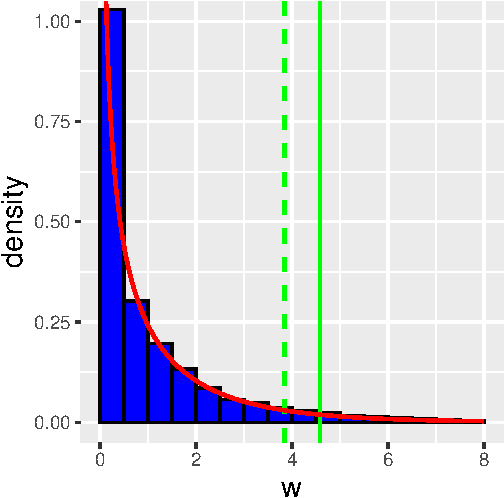
\includegraphics[keepaspectratio]{04-poisson_files/figure-latex/fig-ltrsim-1.pdf}}

}

\caption{\label{fig-ltrsim}The empirical distribution of the statistic
\(-2( \log\mathcal{L}_o - \log\mathcal{L}_a)\), with the chi-square
distribution for \(\Delta r = 1\) degree of freedom overlaid (red
curve). The dashed vertical green line represents the rejection region
boundary according to Wilks' theorem, and the solid vertical green line
represents the 95th percentile of simulated statistic values. The
divergence of the two green lines indicates that Wilks' theorem at best
provides approximate results and that simulations provide more accurate
and precise results as \(n \rightarrow 0\).}

\end{figure}%

\begin{quote}
In this simulation, we find that the empirical rejection-region boundary
is 4.584, which is sufficiently far from the value 3.841 derived from
Wilks' theorem to be concerning. We also find that if we adopt 3.841 as
our boundary value, our Type I error is actually 0.071 instead of the
expected value of 0.05. The upshot: if \(n\) is small, it is best
\emph{not} to assume that \(W\) is chi-square-distributed; run
simulations to determine rejection region boundaries and \(p\)-values
instead.
\end{quote}

\subsubsection{Poisson Distribution: Chi-Square-Based Hypothesis
Testing}\label{poisson-distribution-chi-square-based-hypothesis-testing}

\begin{quote}
In Section~\ref{sec-chap3gof}, we introduced the chi-square
goodness-of-fit test as a way of conducting hypothesis tests given
multinomial data. Given \(k\) data recorded in \(m\) separate bins, we
can compute the test statistic \[
W = \sum_{i=1}^m \frac{(X_i - kp_i)^2}{kp_i} \,,
\] where \(X_i\) is the number of data observed in bin \(i\), and where
\(p_i\) is the probability of any one datum being observed in that bin
under the null. If \(k\) is sufficiently large, then \(W\) converges in
distribution to a chi-square random variable for \(m-1\) degrees of
freedom. (Hence the name of the test!)
\end{quote}

\begin{quote}
But: what if the overall observed number of data \(X\) is a random
variable instead of being a set constant \(X=k\)? Imagine a very simple
digital camera that has four light collecting bins, each of the same
size, and we point it towards a light source that emits an average of
\(\lambda\) photons in a particular time period. If we open the shutter
for that time period, what we would observe is \(X \sim\)
Poisson(\(\lambda\)) photons, with the numbers in each bin being
\(\{X_1,X_2,X_3,X_4\}\). Now let's say we want to test the hypothesis
that the probability of a photon falling into each bin is the same,
i.e., \(H_o: p_1 = p_2 = p_3 = p_4 = 1/4\). If we were to use the
chi-square GoF test directly, we would compute \[
w_{obs} = \sum_{i=1}^4 \frac{(X_i - \lambda p_i)^2}{\lambda p_i} 
\] and then compute the \(p\)-value \(1-F_W(w_{obs})\) assume 3 degrees
of freedom. (In \texttt{R}, this would be computed via
\texttt{1\ -\ pchisq(w.obs,\ 3)}.) We can do this\(-\)the computer will
not stop us from doing so\(-\)but is this valid?
\end{quote}

\begin{quote}
The answer is that this \emph{is} valid so long as each \(X_i\)
converges in distribution to a normal random variable. And Poisson
random variables \emph{do} converge in distribution to normal random
variables, as demonstrated earlier in Section~\ref{sec-chap4pmf}.
Historical convention holds that so long as \(\lambda p_i \geq 5\), we
can utilize the chi-square GoF test given a specific vector of
proportions as a null hypothesis. However, we know that the chi-square
GoF test hinges on the use of a large-sample approximation, specifically
that the test statistic converges in distribution to a chi-square random
variable. So\ldots would it be better to utilize simulations, as we do
when we have multinomial data, to achieve exact \(p\)-values and not
approximate ones? The answer to this question is not as clear-cut here
as it was in Section~\ref{sec-chap3categorical}. In a multinomial
context, \emph{we know the number of trials}, and so we specify the
exact multinomial distribution according to which the data are sampled
under the null hypothesis. Here, \emph{we do not know the true number of
expected counts}; we could make the principled assumption that
\(\lambda = \sum_{i=1}^m X_i\), but that would just be an assumption and
thus any subsequent inference would not be exact (or, more precisely
stated, any inferences that we make would only be exact conditional on
the truth of our assumed value for \(\lambda\), which would comprise one
additional piece of our null hypothesis).
\end{quote}

\begin{quote}
So let's say we want to go ahead and assume a null hypothesis value for
\(\lambda\). What would we do?
\end{quote}

\begin{quote}
First, we would note that under the null, each of our data is
independent and each is sampled from a Poisson distribution: \[
X_i \sim \mbox{Poisson}(\lambda = \lambda_o p_{i,o}) \,.
\] We can straightforwardly run \(m\) separate hypothesis tests. For
instance, if we have four bins with observed data values 9, 12, 6, and
6, and our null hypothesis is
\(H_o : \{ \lambda = \lambda_o = 36, p_{1,o} = \cdots = p_{4,o} = 0.25\}\),
and we are conducting a two-tail test at the level \(\alpha = 0.05\),
then, e.g., the first \(p\)-value would be
\end{quote}

\begin{Shaded}
\begin{Highlighting}[]
\DecValTok{2}\SpecialCharTok{*}\FunctionTok{min}\NormalTok{(}\FunctionTok{c}\NormalTok{(}\FunctionTok{ppois}\NormalTok{(}\DecValTok{9}\NormalTok{, }\DecValTok{36} \SpecialCharTok{*} \FloatTok{0.25}\NormalTok{), }\DecValTok{1} \SpecialCharTok{{-}} \FunctionTok{ppois}\NormalTok{(}\DecValTok{9}\NormalTok{, }\DecValTok{36} \SpecialCharTok{*} \FloatTok{0.25}\NormalTok{)))}
\end{Highlighting}
\end{Shaded}

\begin{verbatim}
[1] 0.8251835
\end{verbatim}

\begin{quote}
How would we then combine the \(m\) \(p\)-values? We can use Fisher's
method, in which we would assume that \[
W = -2 \left( \log p_1 + \cdots + \log p_m \right) 
\] is sampled according to a chi-square distribution for \(2m\) degrees
of freedom under the null. (Recall that each \(p\)-value is, under the
null, sampled from a Uniform(0,1) distribution. We can use this fact
along with the method of transformations to determine that
\(\chi_{2m}^2\) is the \emph{exact} sampling distribution for \(W\)
under the null, not an approximate one.) What do we find?
\end{quote}

\begin{Shaded}
\begin{Highlighting}[]
\NormalTok{m        }\OtherTok{\textless{}{-}} \DecValTok{4}
\NormalTok{X        }\OtherTok{\textless{}{-}} \FunctionTok{c}\NormalTok{(}\DecValTok{9}\NormalTok{, }\DecValTok{12}\NormalTok{, }\DecValTok{6}\NormalTok{, }\DecValTok{6}\NormalTok{)}
\NormalTok{lambda.o }\OtherTok{\textless{}{-}} \DecValTok{36}
\NormalTok{p.o      }\OtherTok{\textless{}{-}} \FunctionTok{rep}\NormalTok{(}\DecValTok{1} \SpecialCharTok{/}\NormalTok{ m, m)}

\NormalTok{p        }\OtherTok{\textless{}{-}} \FunctionTok{rep}\NormalTok{(}\ConstantTok{NA}\NormalTok{, m)}
\NormalTok{W        }\OtherTok{\textless{}{-}} \DecValTok{0}
\ControlFlowTok{for}\NormalTok{ ( ii }\ControlFlowTok{in} \DecValTok{1}\SpecialCharTok{:}\NormalTok{m ) \{}
\NormalTok{  p[ii] }\OtherTok{\textless{}{-}} \DecValTok{2}\SpecialCharTok{*}\FunctionTok{min}\NormalTok{(}\FunctionTok{c}\NormalTok{(}\FunctionTok{ppois}\NormalTok{(X[ii], lambda.o }\SpecialCharTok{*}\NormalTok{ p.o[ii]), }\DecValTok{1} \SpecialCharTok{{-}} \FunctionTok{ppois}\NormalTok{(X[ii], lambda.o }\SpecialCharTok{*}\NormalTok{ p.o[ii])))}
\NormalTok{  W }\OtherTok{\textless{}{-}}\NormalTok{ W }\SpecialCharTok{{-}} \DecValTok{2} \SpecialCharTok{*} \FunctionTok{log}\NormalTok{(p[ii])}
\NormalTok{\}}
\FunctionTok{round}\NormalTok{(}\DecValTok{1} \SpecialCharTok{{-}} \FunctionTok{pchisq}\NormalTok{(W, }\DecValTok{2} \SpecialCharTok{*}\NormalTok{ m), }\DecValTok{3}\NormalTok{)}
\end{Highlighting}
\end{Shaded}

\begin{verbatim}
[1] 0.569
\end{verbatim}

\begin{quote}
The overall \(p\)-value is 0.569; we fail to reject the null hypothesis
that \(\lambda = \lambda_o = 36\) and \(p_1 = p_{1,o} = 0.25\), etc.
\end{quote}

\subsubsection{Death-by-Horse-Kick: Are the Data Poisson
Distributed?}\label{death-by-horse-kick-are-the-data-poisson-distributed}

\begin{quote}
In previous examples, we have shown that over the course of 20 years, in
10 separate Prussian army corps, soldiers died as a result of horse
kicks at a rate of \(\hat{\lambda} = \bar{X} = 0.61\) deaths per corps
per year, and that a 95\% confidence interval for \(\lambda\) is
{[}0.507,0.728{]}. However, we never examined what is perhaps the most
important question of all: is it plausible that the data are
Poisson-distributed in the first place?
\end{quote}

\begin{quote}
In Section~\ref{sec-chap3gof}, we demonstrated how to utilize the
chi-square GoF test as a test of distributions: if we fail to reject the
null, we can assume that it is indeed plausible that a given set of
discrete data are sampled according to the distribution adopted as the
null distribution.
\end{quote}

\begin{quote}
Let's assume \(\lambda = 0.61\). (The estimation of this quantity leads
to the loss of one degree of freedom when we compute the \(p\)-value
below.) Then the probabilities \(P(X=x)\) are as follows:
\end{quote}

{\def\LTcaptype{none} % do not increment counter
\begin{longtable}[]{@{}llll@{}}
\toprule\noalign{}
x & P(X=x) & \(E_x\) & \(O_x\) \\
\midrule\noalign{}
\endhead
\bottomrule\noalign{}
\endlastfoot
0 & 0.543 & 108.67 & 109 \\
1 & 0.331 & 66.29 & 65 \\
2 & 0.101 & 20.29 & 22 \\
3 & 0.021 & 4.11 & 3 \\
4 & 0.003 & 0.63 & 1 \\
\end{longtable}
}

\begin{quote}
The conventional rule-of-thumb is that the expected number of counts in
each bin must be \(\geq 5\). Here, we will break that rule slightly by
combining bins 3 and 4 into one bin with expected counts 4.11 + 0.63 =
4.74. The chi-square GOF test statistic is thus \[
W = \frac{(109-108.67)^2}{108.67} + \frac{(65-66.29)^2}{66.29} + \frac{(22-20.29)^2}{20.29} + \frac{(4-4.74)^2}{4.74} = 0.298 \,.
\] This figure can be found using \texttt{R}:
\end{quote}

\begin{Shaded}
\begin{Highlighting}[]
\NormalTok{e    }\OtherTok{\textless{}{-}} \DecValTok{200} \SpecialCharTok{*} \FunctionTok{dpois}\NormalTok{(}\DecValTok{0}\SpecialCharTok{:}\DecValTok{4}\NormalTok{, }\FloatTok{0.61}\NormalTok{)}
\NormalTok{e[}\DecValTok{4}\NormalTok{] }\OtherTok{\textless{}{-}}\NormalTok{ e[}\DecValTok{4}\NormalTok{] }\SpecialCharTok{+}\NormalTok{ e[}\DecValTok{5}\NormalTok{]}
\NormalTok{e    }\OtherTok{\textless{}{-}}\NormalTok{ e[}\SpecialCharTok{{-}}\DecValTok{5}\NormalTok{]}
\NormalTok{o    }\OtherTok{\textless{}{-}} \FunctionTok{c}\NormalTok{(}\DecValTok{109}\NormalTok{, }\DecValTok{65}\NormalTok{, }\DecValTok{22}\NormalTok{, }\DecValTok{4}\NormalTok{)}

\NormalTok{(W }\OtherTok{\textless{}{-}} \FunctionTok{sum}\NormalTok{((o }\SpecialCharTok{{-}}\NormalTok{ e)}\SpecialCharTok{\^{}}\DecValTok{2} \SpecialCharTok{/}\NormalTok{ e))}
\end{Highlighting}
\end{Shaded}

\begin{verbatim}
[1] 0.2980418
\end{verbatim}

\begin{quote}
When using the chi-square GOF test to assess the viability of a
distribution whose parameters are estimated, we lose additional degrees
of freedom, so the number of degrees of freedom here is 4 - 2 = 2. The
\(p\)-value is
\end{quote}

\begin{Shaded}
\begin{Highlighting}[]
\DecValTok{1} \SpecialCharTok{{-}} \FunctionTok{pchisq}\NormalTok{(W, }\DecValTok{2}\NormalTok{)}
\end{Highlighting}
\end{Shaded}

\begin{verbatim}
[1] 0.8615511
\end{verbatim}

\begin{quote}
We find that we fail to reject the null hypothesis and thus that it is
indeed plausible that Bortkiewicz's horse-kick data are
Poisson-distributed.
\end{quote}

\section{Poisson and Negative Binomial
Regression}\label{sec-chap4poireg}

What to take away from this section:

\begin{itemize}
\item
  Given a set of data tuples \(\{(x_1,Y_1),\ldots,(x_n,Y_n)\}\), where
  the \(x_i\)'s are continuously valued and the \(Y_i\)'s are assumed to
  be Poisson-distributed, we can attempt to determine an association
  between \(\mathbf{x}\) and \(\mathbf{Y}\) by learning a \emph{Poisson
  regression} model (conventionally with the log link function).
\item
  During the data-generating process, it is possible that \(\lambda(x)\)
  can change in value, leading to \emph{overdispersion} (i.e., leading
  to the data having a larger spread in values than a single value of
  \(\lambda(x)\) would suggest).
\item
  To model overdispersed data, we can learn a \emph{negative binomial
  regression} model, which adds an extra parameter to Poisson regression
  that directly indicates the extent to which the data are
  overdispersed.
\end{itemize}

\subsection{Poisson Regression}\label{poisson-regression}

Suppose that for a given measurement \(x\), we record a random variable
\(Y\) that is a number of counts. For instance, \(x\) might be the time
of day, and \(Y\) might be the observed number of cars parked in a lot
at that time. Because \(Y\) is (a) integer valued, and (b) non-negative,
an appropriate distribution for the random variable \(Y\) might be the
Poisson distribution, and thus to model these data, we may want to
pursue the use of Poisson regression.

\smallskip\hrule

\begin{quote}
\textbf{Recall:} \emph{To implement a generalized linear model (or GLM),
we need to do two things:}
\end{quote}

\begin{quote}
\begin{enumerate}
\def\labelenumi{\arabic{enumi}.}
\tightlist
\item
  \emph{examine the \(Y_i\) values and select an appropriate
  distribution for them (discrete or continuous? what is the functional
  domain?); and}
\item
  \emph{define a link function \(g(\theta \vert x)\) that maps the line
  \(\beta_0 + \beta_1 x_i\), which has infinite range, into a more
  limited range (e.g., \((0,\infty)\)).}
\end{enumerate}
\end{quote}

\smallskip\hrule

Because \(\lambda > 0\), in Poisson regression we adopt a link function
that maps \(\beta_0 + \beta_1 x\) from the range \((-\infty,\infty)\) to
\((0,\infty)\). There is no unique choice of link function, but the most
commonly applied one is the logarithm: \[
g(\lambda \vert x) = \log (\lambda \vert x) = \beta_0 + \beta_1 x ~~\implies~~ \lambda(x) = e^{\beta_0 + \beta_1 x} \,.
\] Similar to logistic regression, our goal is to estimate \(\beta_0\)
and \(\beta_1\), which is done via numerical optimization of the
likelihood function \[
\mathcal{L}(\beta_0,\beta_1 \vert \mathbf{y}) = \prod_{i=1}^n p_{Y \vert \beta_0,\beta_1}(y_i \vert \beta_0,\beta_1) = \prod_{i=1}^n \frac{\exp(\beta_0+\beta_1x_i)^{x_i}}{x_i!} e^{-\exp(\beta_0+\beta_1x_i)} \,.
\]

\subsection{Negative Binomial
Regression}\label{negative-binomial-regression}

For the Poisson distribution, \(E[X] = V[X] = \lambda\), so the
expectation is that for any given value \(x\),
\(E[Y \vert x] = V[Y \vert x] = \lambda(x)\). However, it is often
observed in real-life data that the sample variance of \(Y\) exceeds the
sample mean. This is dubbed \emph{overdispersion}, and it can arise
when, e.g., the observed Poisson process is inhomogeneous\ldots or
differently stated, when \(\lambda(x)\) varies as the data are
collected. A standard way to deal with overdispersion is to move from
Poisson regression to \emph{negative binomial regression}.

Before we say more, we will note that while the name ``negative binomial
regression'' is technically correct (in the sense that the model assumes
that the response data are negative binomially distributed), it can be
very confusing for those new to regression, who might view the negative
binomial as a distribution that is only useful when, e.g., modeling
failures in Bernoulli trials. How could that distribution possibly apply
here? The answer is that the negative binomial probability mass function
is ``just'' a function (and as such, it is ``allowed'' to have more
general use than just modeling failures), but more to the point, it is a
function that arises naturally when we apply the Law of Total
Probability to the Poisson pmf.

Let's suppose that \(Y \sim\) Poisson(\(\lambda(x)\)), but that
\(\lambda(x)\) itself is a random variable. There is no unique way to
model its distribution, but the gamma distribution provides a flexible
means by which to do so (since the family encompasses a wide variety of
shapes, unlike, say, the normal distribution, which can never exhibit
skewness). For simplicity, let's assume henceforth that we are looking
at one specific value of \(x\) so that we can drop ``\((x)\)'' from our
notation. If we say that \(\lambda \sim\) Gamma(\(\theta,p/\theta\)),
then we can determine the distribution of \(Y\) is found with the LoTP:
\begin{align*}
p_{Y \vert \theta,p}(y \vert \theta,p) &= \int_0^\infty p_{Y \vert \lambda}(y \vert \lambda) f_{\lambda}(\lambda \vert \theta,p) d\lambda \\
&= \int_0^\infty \frac{\lambda^y}{y!} e^{-\lambda} \frac{\lambda^{\theta-1}}{(p/\theta)^\theta} \frac{e^{-\lambda/(p/\theta)}}{\Gamma(\theta)} d\lambda \\
&= \frac{1}{y!}\left(\frac{\theta}{p}\right)^\theta \frac{1}{\Gamma(\theta)} \int_0^\infty \lambda^{y+\theta+1} e^{-\lambda(1+\theta/p)} d\lambda \,.
\end{align*} The integrand looks suspiciously like the integrand of a
gamma function integral, but we have to change \(\lambda(1+\theta/p)\)
in the exponential to just \(\lambda'\): \[
\lambda' = \lambda(1+\theta/p) ~~ \mbox{and} ~~ d\lambda' = d\lambda (1+\theta/p) \,.
\] The bounds of the integral do not change. The integral now becomes
\begin{align*}
p_{Y \vert \theta,p}(y \vert \theta,p) &= \frac{1}{y!}\left(\frac{\theta}{p}\right)^\theta \frac{1}{\Gamma(\theta)} \frac{1}{(1+\theta/p)^{y+\theta}} \int_0^\infty (\lambda')^{y+\theta-1} e^{-\lambda'} d\lambda' \\
&= \frac{1}{y!}\left(\frac{\theta}{p}\right)^\theta \frac{1}{\Gamma(\theta)} \frac{1}{(1+\theta/p)^{y+\theta}} \Gamma(y+\theta) \\
&= \frac{(y+\theta-1)!}{y! (\theta-1)!} \left(\frac{\theta}{p}\right)^\theta \left(\frac{p}{p+\theta}\right)^{y+\theta} \\
&= \binom{y+\theta-1}{y} \left(\frac{p}{p+\theta}\right)^y \left(\frac{\theta}{p}\right)^\theta \left(\frac{p}{p+\theta}\right)^\theta \\
&= \binom{y+\theta-1}{y} \left(\frac{p}{p+\theta}\right)^y \left(\frac{\theta}{p+\theta}\right)^\theta \\
&= \binom{y+\theta-1}{y} \left(\frac{\theta}{p+\theta}\right)^\theta \left(1 - \frac{\theta}{p+\theta}\right)^y \,.
\end{align*} This has the functional form of a negative binomial pmf in
which \(y\) represents the number of ``failures,'' \(\theta\) is the
number of ``successes,'' and \(\theta/(p+\theta)\) is the probability of
success.

Now, why do we choose this form of the negative binomial distribution?
We do so because it so happens that \begin{align*}
E[Y] &= p \\
V[Y] &= p + \frac{p^2}{\theta} \,.
\end{align*} (One can derive these quantities starting with, e.g.,
\(E[Y] = \theta(1-p')/p'\) and \(V[Y] = \theta(1-p')/(p')^2\) and
plugging in \(p' = \theta/(p+\theta)\).) Varying \(\theta\) thus allows
us to model the overdispersion with a single variable. We assume that
\(p\) takes the place of \(\lambda\), in the sense that now
\(p = \exp(\beta_0 + \beta_1x\)) for our given specific value of \(x\).
In the limit that \(\theta \rightarrow \infty\), negative binomial
regression becomes Poisson regression. Because the overdispersion is
represented in a single variable, we can examine the results of learning
both Poisson and negative binomial regression models to determine
whether or not the quality of fit improves enough to justify additional
model complexity.

For a deeper dive into Poisson and negative binomial regression, see,
e.g., Chapter 4 of Roback and Legler (2021).

\subsection{Examples}\label{examples-43}

\subsubsection{Poisson Regression:
Example}\label{poisson-regression-example}

\begin{quote}
In the code chunk below, we simulate 100 data at each of four different
values of \(x\): 1, 2, 3, and 4. The data are simulated with a Poisson
overdispersion factor of 2.
\end{quote}

\begin{Shaded}
\begin{Highlighting}[]
\FunctionTok{set.seed}\NormalTok{(}\DecValTok{236}\NormalTok{)}
\NormalTok{n }\OtherTok{\textless{}{-}} \DecValTok{100}               \CommentTok{\# 100 data per x value}
\NormalTok{x }\OtherTok{\textless{}{-}} \FunctionTok{rep}\NormalTok{(}\FunctionTok{c}\NormalTok{(}\DecValTok{1}\NormalTok{, }\DecValTok{2}\NormalTok{, }\DecValTok{3}\NormalTok{, }\DecValTok{4}\NormalTok{), n)}
\NormalTok{Y }\OtherTok{\textless{}{-}} \FunctionTok{rep}\NormalTok{(}\ConstantTok{NA}\NormalTok{, }\FunctionTok{length}\NormalTok{(x))}
\ControlFlowTok{for}\NormalTok{ ( ii }\ControlFlowTok{in} \DecValTok{1}\SpecialCharTok{:}\FunctionTok{length}\NormalTok{(x) ) \{}
\NormalTok{  Y[ii] }\OtherTok{\textless{}{-}} \FunctionTok{rpois}\NormalTok{(}\DecValTok{1}\NormalTok{, }\FunctionTok{rgamma}\NormalTok{(}\DecValTok{1}\NormalTok{, }\DecValTok{2}\NormalTok{, }\AttributeTok{scale =}\NormalTok{ x[ii] }\SpecialCharTok{/} \DecValTok{2}\NormalTok{))}
\NormalTok{\}}
\end{Highlighting}
\end{Shaded}

For these data, \(E[Y|x] = x\) and \(V[Y|x] = x + x^2/2\), meaning that
the overdispersion factor is, again, \(\theta = 2\). Let's see how
overdispersion affects the learning of a Poisson regression model. (And
then below we'll see how much our ability to model these data improves
if we learn a negative binomial regression model.)

\begin{Shaded}
\begin{Highlighting}[]
\NormalTok{poi.out }\OtherTok{\textless{}{-}} \FunctionTok{glm}\NormalTok{(Y }\SpecialCharTok{\textasciitilde{}}\NormalTok{ x, }\AttributeTok{family =}\NormalTok{ poisson)}
\FunctionTok{print}\NormalTok{(}\StringTok{"Deviance Residuals"}\NormalTok{)}
\end{Highlighting}
\end{Shaded}

\begin{verbatim}
[1] "Deviance Residuals"
\end{verbatim}

\begin{Shaded}
\begin{Highlighting}[]
\FunctionTok{summary}\NormalTok{(}\FunctionTok{residuals}\NormalTok{(poi.out))}
\end{Highlighting}
\end{Shaded}

\begin{verbatim}
   Min. 1st Qu.  Median    Mean 3rd Qu.    Max. 
-2.9013 -1.6404 -0.3122 -0.2726  0.6825  5.6697 
\end{verbatim}

\begin{Shaded}
\begin{Highlighting}[]
\FunctionTok{summary}\NormalTok{(poi.out)}
\end{Highlighting}
\end{Shaded}

\begin{verbatim}

Call:
glm(formula = Y ~ x, family = poisson)

Coefficients:
            Estimate Std. Error z value Pr(>|z|)    
(Intercept) -0.08336    0.09240  -0.902    0.367    
x            0.38014    0.02944  12.913   <2e-16 ***
---
Signif. codes:  0 '***' 0.001 '**' 0.01 '*' 0.05 '.' 0.1 ' ' 1

(Dispersion parameter for poisson family taken to be 1)

    Null deviance: 1107  on 399  degrees of freedom
Residual deviance:  930  on 398  degrees of freedom
AIC: 1805

Number of Fisher Scoring iterations: 5
\end{verbatim}

\begin{quote}
The summary output from the Poisson regression model is, in its
structure, identical to that of logistic regression. But there are some
differences in how values are defined. For instance, the deviance
residual is \[
d_i = \mbox{sign}(Y_i - \hat{Y}_i) \sqrt{2[Y_i \log (Y_i/\hat{Y}_i) - (Y_i - \hat{Y}_i)]} \,,
\] where \[
\hat{Y}_i = \hat{\lambda}_i = \exp(\hat{\beta}_0+\hat{\beta}_1 x_i) \,.
\] (Note that when \(Y_i = 0\), \(Y_i \log (Y_i/\hat{Y}_i)\) is assumed
to be zero as well.) Also, the residual deviance (here, 930) is
\emph{not} \(-2 \log \mathcal{L}_{max}\), as it was for logistic
regression. To determine \(\log \mathcal{L}_{max}\), we note that \[
{\mathrm{AIC}} = -2 \log \mathcal{L}_{max} + 2 k \,,
\] where \(k\) is the number of model terms (here, two). Alternatively,
we can utilize the \texttt{logLik()} function:
\end{quote}

\begin{Shaded}
\begin{Highlighting}[]
\FunctionTok{round}\NormalTok{(}\FunctionTok{logLik}\NormalTok{(poi.out), }\DecValTok{3}\NormalTok{)}
\end{Highlighting}
\end{Shaded}

\begin{verbatim}
'log Lik.' -900.518 (df=2)
\end{verbatim}

\begin{quote}
As we did in the context of logistic regression, we can use the the
difference in the values of the null and residual deviances (here, 1107
- 930 = 177) to test the null hypothesis that \(\beta_1 = 0\). The
difference is assumed to be sampled according to a chi-square
distribution for 4-3 = 1 degree of freedom. The \(p\)-value is
\texttt{1\ -\ pchisq(177,\ 1)} or effectively zero: we emphatically
reject the null hypothesis that \(\beta_1 = 0\).
\end{quote}

\begin{quote}
As a final note, unlike the case of logistic regression where
determining the quality of fit of the learned model is not particularly
straightforward, for Poisson regression we can simply assume that the
residual deviance is chi-square-distributed for the given number of
degrees of freedom. Here, the \(p\)-value is
\end{quote}

\begin{Shaded}
\begin{Highlighting}[]
\FunctionTok{round}\NormalTok{(}\DecValTok{1} \SpecialCharTok{{-}} \FunctionTok{pchisq}\NormalTok{(}\DecValTok{930}\NormalTok{, }\DecValTok{398}\NormalTok{), }\DecValTok{5}\NormalTok{)}
\end{Highlighting}
\end{Shaded}

\begin{verbatim}
[1] 0
\end{verbatim}

\begin{quote}
or, again, effectively zero. Because this value is less than, e.g.,
\(\alpha = 0.05\), we would reject the null hypothesis that the observed
data are truly Poisson distributed.
\end{quote}

\subsubsection{Negative Binomial Regression:
Example}\label{negative-binomial-regression-example}

\begin{quote}
At the conclusion of the previous example, we observed that by the
metric of residual deviance, the data we are analyzing are not truly
Poisson distributed. However, is it plausible that the data simply
exhibit overdispersion? Here we will find out, by carrying out negative
binomial regression with the \texttt{glm.nb()} function of the
\texttt{MASS} package. (``MASS'' stands for ``Modern Applied Statistics
with S''\ldots with \texttt{S} being the precursor software to
\texttt{R}.)
\end{quote}

\begin{Shaded}
\begin{Highlighting}[]
\FunctionTok{suppressMessages}\NormalTok{(}\FunctionTok{library}\NormalTok{(MASS))}

\NormalTok{nb.out }\OtherTok{\textless{}{-}} \FunctionTok{suppressWarnings}\NormalTok{(}\FunctionTok{glm.nb}\NormalTok{(Y }\SpecialCharTok{\textasciitilde{}}\NormalTok{ x))}
\FunctionTok{print}\NormalTok{(}\StringTok{"Deviance Residuals"}\NormalTok{)}
\end{Highlighting}
\end{Shaded}

\begin{verbatim}
[1] "Deviance Residuals"
\end{verbatim}

\begin{Shaded}
\begin{Highlighting}[]
\FunctionTok{summary}\NormalTok{(}\FunctionTok{residuals}\NormalTok{(nb.out))}
\end{Highlighting}
\end{Shaded}

\begin{verbatim}
   Min. 1st Qu.  Median    Mean 3rd Qu.    Max. 
-2.1019 -1.2027 -0.2295 -0.2886  0.4198  2.8666 
\end{verbatim}

\begin{Shaded}
\begin{Highlighting}[]
\FunctionTok{summary}\NormalTok{(nb.out)}
\end{Highlighting}
\end{Shaded}

\begin{verbatim}

Call:
glm.nb(formula = Y ~ x, init.theta = 1.84882707, link = log)

Coefficients:
            Estimate Std. Error z value Pr(>|z|)    
(Intercept) -0.10769    0.13101  -0.822    0.411    
x            0.38908    0.04483   8.679   <2e-16 ***
---
Signif. codes:  0 '***' 0.001 '**' 0.01 '*' 0.05 '.' 0.1 ' ' 1

(Dispersion parameter for Negative Binomial(1.8488) family taken to be 1)

    Null deviance: 530.52  on 399  degrees of freedom
Residual deviance: 454.45  on 398  degrees of freedom
AIC: 1633.9

Number of Fisher Scoring iterations: 1

              Theta:  1.849 
          Std. Err.:  0.258 

 2 x log-likelihood:  -1627.868 
\end{verbatim}

\begin{quote}
When we compare the output, we first look for the lines beginning with
\texttt{AIC}:
\end{quote}

\begin{verbatim}
AIC: 1805.0  [Poisson regression]
AIC: 1633.9  [negative binomial regression]
\end{verbatim}

\begin{quote}
The Akaike Information Criterion, or AIC, as we will recall, is a
quality-of-fit metric that penalizes model complexity. If we learn a
suite of models, we would generally adopt that associated with the
lowest AIC value. Here, the negative binomial model has a lower AIC
value than the Poisson model, so we would adopt that model.
But\ldots can we say the negative binomial model a good model in an
absolute sense? To determine that, we would compare the residual
deviance value of 454.45 against a chi-square distribution with 398
degrees of freedom; the result is
\end{quote}

\begin{Shaded}
\begin{Highlighting}[]
\FunctionTok{round}\NormalTok{(}\DecValTok{1} \SpecialCharTok{{-}} \FunctionTok{pchisq}\NormalTok{(}\FloatTok{454.45}\NormalTok{, }\DecValTok{398}\NormalTok{), }\DecValTok{4}\NormalTok{)}
\end{Highlighting}
\end{Shaded}

\begin{verbatim}
[1] 0.0264
\end{verbatim}

\begin{quote}
Technically, we reject the null hypothesis and conclude that the
negative binomial model is a not a plausible representation of the
data-generating process. However, given that the \(p\)-value is close to
0.05, we feel that we can state that the model is potentially plausible
and can continue to interpret its properties, while being cautious not
to ``oversell'' its viability.
\end{quote}

\begin{quote}
The estimated value of the overdispersion parameter is
\(\hat{\theta} = 1.849\), with estimated standard error \(0.258\). This
result clearly indicates that the data exhibit overdispersion.
\end{quote}

\section{Exercises}\label{sec-chap4exercises}

\begin{enumerate}
\def\labelenumi{\arabic{enumi}.}
\item
  Suppose that you receive phone calls at a rate of 2 per hour. (a) Let
  \(X\) be the number of phone calls received in a randomly selected
  15-minute period. Compute \(P(\mu \leq X \leq \mu+2\sigma)\). (b) Let
  \(Y\) be the length of time between when the phone first rings from
  one call and when the phone first rings for the next call. What is
  \(P(Y > 1/2 \, \vert \, Y > 1/4)\)? (c) When the phone rings, there is
  probability 0.2 that the caller is your friend, who you always talk to
  for 10 minutes. (All other calls are one minute in length.) What is
  the expected overall time spent on the phone during any given set of
  10 phone calls?
\item
  A particular basketball player shoots, \emph{on average}, one time
  every two minutes, and exactly half of her shots are successful. In an
  upcoming game, she is to play for exactly eight minutes. (a) What is
  the probability that the player will have one successful shot, or
  less? (b) What is the probability that the number of successful shots
  will be within one standard deviation of the mean?
\item
  A particular event happens, on average, three times per year in
  California, four times per year in Nevada, and one time per year in
  Arizona. Instances of these events are independent of each other. What
  the mean and variance for the total number of events, summed over the
  three states, that would be observed in a single two-year window of
  time?
\item
  We sample \(n\) iid data from the following distribution:
  \begin{align*}
  f_X(x) = \frac{x}{\sigma^2} e^{-x^2/(2\sigma^2)} \,,
  \end{align*} where \(x \geq 0\) and \(\sigma > 0\). For this
  distribution, \(E[X] = \sigma\sqrt{\pi/2}\) and
  \(V[X] = (4-\pi)\sigma^2/2\). (a) What is \(E[X^2]\)? (b) What is the
  method of moments estimator for \(\sigma\) that utilizes the first
  population and sample moments? (c) What is the bias of
  \(\hat{\sigma}_{MoM}\)? (d) What is the variance of
  \(\hat{\sigma}_{MoM}\)? (e) What is the method of moments estimator of
  \(\sigma^2\) that utilizes the \emph{second} population and sample
  moments?
\item
  We sample a datum \(X\) from a geometric distribution. (a) Find a
  method-of-moments estimator of \(p\), based on the first population
  and sample moments. (b) Find a second method-of-moments estimator of
  \(p\), using the second moments.
\item
  We sample \(n\) iid data from a beta distribution with \emph{known}
  value \(\alpha\). (a) Write down the method-of-moments estimator for
  \(\beta\) that is based on the first sample moment. (b) Can we use our
  answer to part (a) to write down the method-of-moments estimator for
  \(\sqrt{\beta}\)? If yes, write down that estimator.
\item
  We have been given the code shown below for computing a 95\% one-sided
  lower bound on \(\lambda\), given \(n\) iid data sampled according to
  a Poisson distribution. Apparently someone was in a hurry. (a) Is the
  argument list for \texttt{f} valid as is? If not, specify how it
  should be fixed. (b) Is the input to \texttt{ppois()} valid as is? If
  not, specify how it should be fixed. (c) The code writer forgot to
  ``FIX'' the input value of \texttt{q} in the \texttt{uniroot()} call.
  Specify the number that should go here. (d) Will the coverage of the
  confidence intervals found with a properly fixed code be exactly 95\%,
  greater than or equal to 95\%, or less than or equal to 95\%?
\end{enumerate}

\begin{verbatim}
X <- ... # this is a vector of n iid Poisson r.v.'s
n <- length(X)
f <- function(X, lambda, n, q)
{
  ppois(mean(X), lambda) - q
}
uniroot(f, interval = c(0.001, 1000), X = X, n = n, q = FIX)$root
\end{verbatim}

\begin{enumerate}
\def\labelenumi{\arabic{enumi}.}
\setcounter{enumi}{7}
\item
  The Bernoulli probability mass function is \begin{align*} 
  p_X(x) = p^x (1-p)^{1-x} \,,
  \end{align*} where \(x \in \{0,1\}\) and \(p \in (0,1)\). Assume that
  we draw \(n\) iid data from this distribution. (a) Write down the
  likelihood ratio test statistic \(\lambda_{LR}\) that arises when
  testing the hypothesis \(H_o : p = p_o\) versus the hypothesis
  \(H_a : p \neq p_o\). (b) In this situation, is the LRT the most
  powerful test?
\item
  In an experiment, you sample \emph{one datum} from a Poisson
  distribution; the value of that datum is \(x_{\mathrm{obs}}\). You
  wish to test \(H_o : \lambda = \lambda_o\) versus the alternative
  \(H_a : \lambda \neq \lambda_o\), and you will do this by utilizing
  the likelihood ratio test. However, instead of identifying a
  sufficient statistic and constructing an exact test, you decide to use
  Wilks' theorem. (In real life: don't do this\ldots construct an exact
  test.) (a) Write down \(\hat{\lambda}_{MLE}\). (b) Write down an
  expression for \(\lambda_{LR}\). (c) Use the answer for part (a) to
  write down an expression for the Wilks' theorem test statistic. (d)
  Regarding the statistic written down for part (c): what is its
  sampling distribution? Give the name and the values of its parameters.
\item
  In an experiment, you sample \(n\) iid data from a Poisson
  distribution with unknown mean \(\lambda\). You wish to conduct a
  likelihood-ratio test for which \(H_a : \lambda < \lambda_o\). Assume
  \(\alpha = 0.05\). (a) Write down the sufficient statistic for
  \(\lambda\) that appears directly in likelihood factorization. (b)
  Write down the sampling distribution for the statistic you found in
  part (a), the name and the value(s) of its parameters. (c) Write down
  the appropriate null hypothesis, given the stated alternative (and
  given that you are performing an LRT). (d) Write down the rejection
  region, using \texttt{R} code (e.g.,
  \texttt{qnorm(0.975,\ mean\ =\ mu.o,\ sd\ =\ sqrt(sigma2))}). Assume
  the null value is to be written as \texttt{lambda.o}, and that a
  number should be provided for \(q\).
\item
  You are given \(n\) iid data sampled according to an exponential
  distribution with pdf \begin{align*}
  f_X(x \vert \beta) = \frac{1}{\beta}e^{-x/\beta} \,,
  \end{align*} where \(x > 0\) and \(\beta > 0\). (a) We wish to test
  \(H_o : \beta = 1\) versus \(H_a : \beta \neq 1\) at level
  \(\alpha = 0.05\). Write down an expression for the likelihood ratio
  test statistic \(\lambda\). Recall that the MLE for \(\beta\) is
  \(\bar{X}\). (b) Assume that you do not know the sampling distribution
  for any sufficient statistic that you can define. Use Wilks' theorem
  to write down a rejection region for this test.
\item
  Suppose you flipped a coin 1000 times and observe heads 550 times. You
  wish to conduct a likelihood-ratio test to check whether this coin is
  fair, at the level \(\alpha = 0.05\). (a) Specify the null and
  alternative hypotheses. (b) What are the corresponding sets
  \(\Theta_0\) and \(\Theta_a\)? (c) Determine the number of free
  parameters \(r_0\) and \(r\) in \(\Theta_0\) and
  \(\Theta = \Theta_0\, \cup\, \Theta_a\), respectively. (d) Determine
  the likelihood ratio test statistic, and its value for the observed
  data. (e) Assume that you do not know the sampling distribution for
  any sufficient statistic that you can define, and use Wilks' theorem
  to determine the corresponding \(p\)-value. (f) Give your conclusion.
  Is the coin fair?
\item
  You are given the following probability density function:
  \begin{align*}
  f_X(x) = \left\{ \begin{array}{cl} \frac{27}{16} x^2 e^{-\frac{3x}{2}} & x > 0 \\ 0 & \mbox{otherwise} \end{array} \right. \,.
  \end{align*} What are \(E[X]\) and \(V[X]\)?
\item
  Assume you are working with a gamma distribution for which
  \(E[X] = 5\) and \(V[X] = 10\). (a) What are the values of \(\alpha\)
  and \(\beta\)? (b) What other name is given to this particular
  distribution, given the values of \(\alpha\) and \(\beta\) you derived
  in (a)?
\item
  Compute \(E[X^{-1}]\) for a chi-square distribution, leaving your
  answer in terms of the number of degrees of freedom \(\nu\).
\item
  The inverse-gamma distribution has the probability density function
  \begin{align*}
  f_X(x) = \frac{\beta^\alpha}{\Gamma(\alpha)} \frac{1}{x^{\alpha+1}} e^{-\beta/x} \,,
  \end{align*} for \(x > 0\) and \(\alpha,\beta > 0\). Derive \(E[X]\)
  for this distribution. Your final answer should be in terms of
  \(\alpha\) and \(\beta\) only (with no gamma or beta functions
  appearing in the answer).
\item
  Let \(X\) be a random variable sampled according to a
  Gamma(3/2,\(\beta\)) distribution. (a) If \(\beta = 2\), what
  sub-family of gamma distributions is \(X\) sampled from? (b) Now,
  assume \(\beta\) is unknown, and that we sample \(n\) iid random
  variables \(\{X_1,\ldots,X_n\}\). What is a sufficient statistic for
  \(\beta\)? (c) What is the MVUE for \(\beta\)? (d) What is the method
  of moments estimator for \(\beta\) that utilizes the first population
  and sample moments? (e) What is the bias of \(\hat{\beta}_{MoM}\)?
\item
  What is \(E[X^{1/2}]\) for the random variable \(X \sim\)
  Gamma(\(\alpha,\beta\))?
\item
  Below is (edited) output from the application of Poisson and negative
  binomial regression to a dataset in \texttt{R}:
\end{enumerate}

\begin{center}
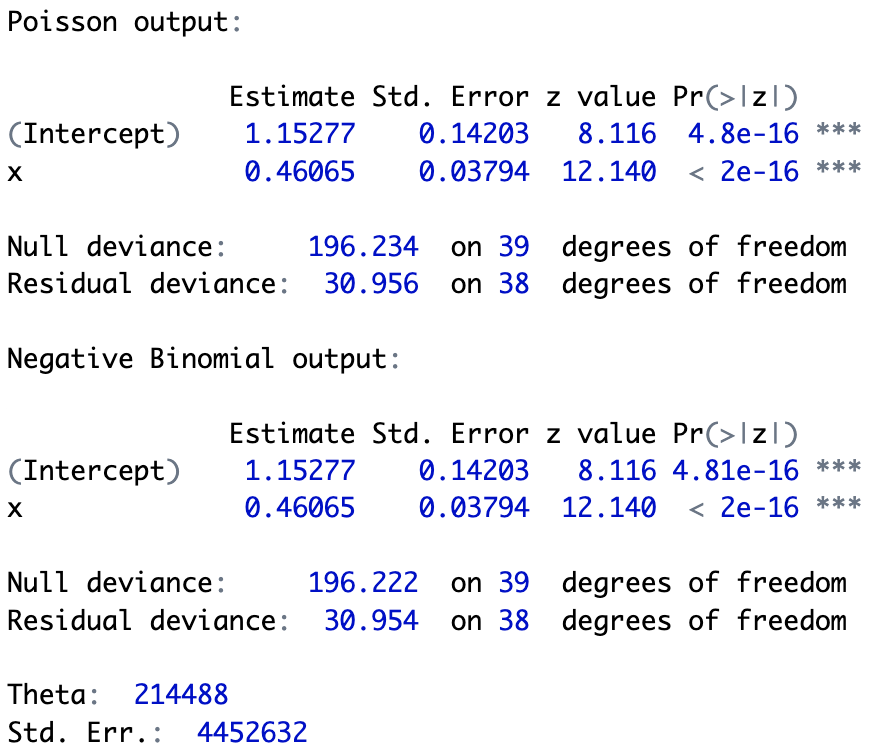
\includegraphics[width=0.7\linewidth,height=\textheight,keepaspectratio]{figures/PoiNB.png}
\end{center}

(a) Identify the value for the overdispersion parameter. (b) Is the
value of the overdispersion parameter such that we can conclude that the
data are indeed overdispersed? (c) What procedure utilizes the two
deviance values in each model to make inferences about one or more of
the model coefficients? (d) What specific conclusion can we make given
both the procedure in (c) and the deviance values that are observed?
Recall what the null and alternative hypotheses are, and state a
conclusion based on these and the observed deviance values.

\begin{center}\rule{0.5\linewidth}{0.5pt}\end{center}

\begin{enumerate}
\def\labelenumi{\arabic{enumi}.}
\setcounter{enumi}{19}
\item
  We sample 100 iid data from a Gamma(1,1). (a) What is the sampling
  distribution for \(\bar{X}\)? (Provide the name of the distribution
  and its parameter value(s).) (b) Using \texttt{R}, determine
  \(P(\bar{X} \geq E[X])\).
\item
  The entropy and the probability-generating function for a discrete
  distribution are given by \(E[-\log p_X(X)]\) and \(E[z^X]\)
  respectively. (a) Write down an evaluated expression for the entropy
  of a Poisson distribution. Do not evaluate \(E[X!]\) and/or
  \(E[\log X!]\) if they appear. (b) Write down an evaluated expression
  for the probability-generating function of a Poisson distribution.
\item
  We are given the following probability density function:
  \begin{align*}
  f_X(x) = 4x^2e^{-2x} ~~~~~~ x \geq 0 \,.
  \end{align*} (a) \(f_X(x)\) belongs to what family of distributions
  that we have studied in class? Just provide the name. (b) What are the
  parameter value(s) for this distribution? (c) Determine \(E[X]\).
\item
  A half-normal distribution has expected value \(\sigma\sqrt{2/\pi}\)
  and variance \(\sigma^2(1-2/\pi)\). (a) What is the method-of-moments
  estimator for \(\sigma\) that is based on the first population and
  sample moments? (b) What is the method-of-moments estimator for
  \(\sigma^2\) that is based on the second population and sample
  moments?
\item
  In an experiment, we sample \emph{one datum} according to the
  following unnamed distribution: \begin{align*}
  f_X(x) = \frac{\theta}{3^\theta} x^{\theta-1} ~~~~~~ x \in [0,3] ~~~~~~ \theta > 0 \,.
  \end{align*} We then test the hypothesis \(H_o : \theta = \theta_o\)
  versus \(H_a : \theta \neq \theta_o\) at level \(\alpha\). (a) What is
  the maximum likelihood estimate for \(\theta\)? (b) Write down the
  likelihood-ratio test statistic \(\lambda_{\mathrm{LR}}\). Leave the
  symbol \(\hat{\theta}_{MLE}\) in the answer. (c) We decide that we
  will utilize Wilks' theorem to compute the \(p\)-value for the test.
  Write down an expression for the test statistic. Again, leave
  \(\hat{\theta}_{MLE}\) in the answer. (d) Write down the \texttt{R}
  function call that would return the \(p\)-value (in the context of
  using Wilks' theorem). Assume the statistic is stored as the variable
  \texttt{stat}. If there are one or more additional arguments to the
  function, specify its/their numerical value(s).
\item
  Below we show the output from when we learn two separate models, given
  the same data. (a) Identify the specific type of generalized linear
  model whose output is shown to the right. (b) Which model, the one to
  the left or the one to the right, should we select as the better
  representation of the data-generating process, and why? As for the
  ``why,'' point out a specific metric that we would use to make our
  choice. (c) Is the model to the left a valid representation of the
  data-generating process? Write down an \texttt{R} function call that
  would return a metric that would allow us to decide ``yes'' or ``no.''
\end{enumerate}

\begin{verbatim}
            Estimate Std. Error z value Pr(>|z|)                        Estimate Std. Error z value Pr(>|z|)
(Intercept)  1.02442    0.15411   6.647 2.98e-11 ***        (Intercept)   1.0090     0.1733   5.823 5.79e-09 ***
x            0.46731    0.05674   8.236  < 2e-16 ***        x             0.4747     0.0676   7.023 2.17e-12 ***

    Null deviance: 111.21  on 29  degrees of freedom            Null deviance: 82.671  on 29  degrees of freedom
Residual deviance:  41.94  on 28  degrees of freedom        Residual deviance: 31.527  on 28  degrees of freedom
AIC: 152.92                                                 AIC: 153.07

                                                                          Theta:  21.5
                                                                      Std. Err.:  20.9
\end{verbatim}

\bookmarksetup{startatroot}

\chapter{Distributions with Domain-Specifying
Parameters}\label{sec-chap5}

Let \(\{X_1,\ldots,X_n\}\) be \(n\) independent and identically
distributed data sampled according to a distribution \(P(\theta)\).

\begin{itemize}
\tightlist
\item
  \(\theta\) is a \emph{domain-specifying parameter} if, e.g., all the
  sampled data have values \(\leq \theta\).
\end{itemize}

This chapter is all about the quirks that we observe when we work with
domain-specifying parameters, ones that affect the determination of
maximum-likelihood and minimum-variance unbiased estimators, how we go
about constructing hypothesis tests, etc.

\section{Distribution Examples}\label{sec-chap5examples}

What to take away from this section:

\begin{itemize}
\item
  While there are many distributions that feature domain-specifying
  parameters, in this chapter we will focus our attention on two:

  \begin{itemize}
  \item
    the \emph{uniform} distribution, a finite distribution whose
    probability density function has the domain \([a,b]\); and
  \item
    the \emph{Pareto} distribution, a semi-infinite distribution whose
    pdf has the domain \([b,\infty)\).
  \end{itemize}
\end{itemize}

Many probability distributions have parameters that bound their domain.
In this chapter, we will concentrate on two in particular that are often
used in inferential analyses:

\begin{itemize}
\tightlist
\item
  the \emph{uniform} distribution; and
\item
  the \emph{Pareto} distribution.
\end{itemize}

\subsection{Uniform Distribution}\label{sec-chap5uniform}

The uniform distribution is often used within the realm of probability,
in part because of its utility and in part because of its simplicity. We
have touched upon this distribution previously, such as when we
discussed how hypothesis test \(p\)-values are distributed uniformly
between 0 and 1 when the null hypothesis is correct. Why do we return to
the uniform distribution now? Because it is slightly different from
other distributions: its two parameters, often denoted \(a\) and \(b\)
(where \(b > a\)), do not dictate the shape of its probability density
function, but rather its domain.

\smallskip\hrule

\begin{quote}
\textbf{Recall}: \emph{a probability density function is one way to
represent a continuous probablity distribution, and it has the
properties (a) \(f_X(x) \geq 0\) and (b) \(\int_x f_X(x) dx = 1\), where
the integral is over all values of \(x\) in the distribution's domain.}
\end{quote}

\smallskip\hrule

The uniform pdf is defined as \[
f_X(x) = \frac{1}{b-a} \,,
\] where \(x \in [a,b]\); \(f_X(x)\) is thus constant between \(a\) and
\(b\). (See Figure~\ref{fig-unifpdf}).) This means that we can think of
the uniform distribution ``geometrically,'' as the following is true: \[
\underbrace{(b-a)}_{\mbox{domain}} \cdot \underbrace{\frac{1}{b-a}}_{f_X(x)} = 1
\] If we know the domain of the pdf, we immediately know \(f_X(x)\);
conversely, if we know \(f_X(x)\), we immediately know the width of the
domain (but not \(a\) and \(b\) themselves).

\begin{figure}

\centering{

\pandocbounded{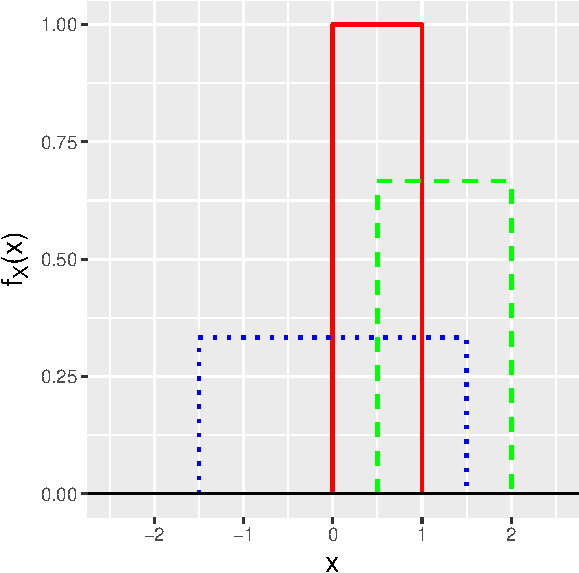
\includegraphics[keepaspectratio]{05-uniform_files/figure-latex/fig-unifpdf-1.pdf}}

}

\caption{\label{fig-unifpdf}Three examples of uniform probability
density functions: Uniform(0,1) (solid red line), Uniform(0.5,2) (dashed
green line), and Uniform(-1.5,1.5) (dotted blue line).}

\end{figure}%

\smallskip\hrule

\begin{quote}
\textbf{Recall}: \emph{the cumulative distribution function, or cdf, is
another means by which to encapsulate information about a probability
distribution. For a continuous distribution, it is defined as
\(F_X(x) = \int_{y \leq x} f_Y(y) dy\), and it is defined for all values
\(x \in (-\infty,\infty)\), with \(F_X(-\infty) = 0\) and
\(F_X(\infty) = 1\).}
\end{quote}

\smallskip\hrule

The cdf for a uniformly distributed random variable is \[
F_X(x) = \int_a^x f_Y(y) dy = \int_a^x \frac{1}{b-a} dy = \frac{x-a}{b-a} ~~ x \in [a,b] \,,
\] with a value of 0 for \(x < a\) and 1 for \(x > b\). (We can quickly
confirm that the derivative of the cdf yields the pdf. Recall that for
continuous distributions, \(f_X(x) = dF_X(x)/dx\).)

\smallskip\hrule

\hrule

\begin{quote}
\textbf{Recall}: \emph{an inverse cdf function \(F_X^{-1}(q)\) takes as
input a distribution quantile \(q \in [0,1]\) and returns the value of
\(x\) such that \(q = F_X(x)\).}
\end{quote}

\smallskip\hrule

The inverse cdf is exceptionally simple to compute: \[
q = \frac{x-a}{b-a} ~~ \Rightarrow ~~ x = (b-a)q + a \,.
\]

\subsection{Pareto Distribution}\label{sec-chap5pareto}

The Pareto {[}puh-RAY-toh{]} distribution, also known as the power-law
distribution, has the probability density function \[
f_X(x) = \frac{a b^a}{x^{a+1}} \,,
\] where \(a > 0\) and \(x \in [b,\infty)\). \(b\) is thus a
domain-specifying parameter. See Figure~\ref{fig-parpdf}. Many phenomena
are linked to this distribution\(-\)the sizes of asteroids in the Solar
System, the sizes of human settlements, personal wealth, etc.\(-\)and it
is popularly known for spawning the so-called ``80-20 rule'': e.g., 80\%
of wealth is tied to 20\% of the population. (Note that this rule is
linked to a specific value of \(a\) and is not meant to be taken as an
iron-clad law that spans across disciplines.)

\begin{figure}

\centering{

\pandocbounded{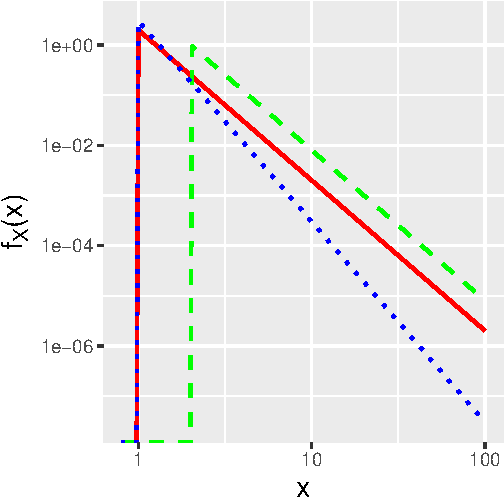
\includegraphics[keepaspectratio]{05-uniform_files/figure-latex/fig-parpdf-1.pdf}}

}

\caption{\label{fig-parpdf}Three examples of Pareto probability density
functions: Pareto(\(a\)=2, \(b\)=1) (solid red line), Pareto(\(a\)=3,
\(b\)=1) (dashed green line), and Pareto(\(a\)=2, \(b\)=2) (dotted blue
line). Note that the pdfs are displayed on a log-log scale, given how
quickly they decrease towards zero.}

\end{figure}%

The cdf for a Pareto distribution is \[
F_X(x) = 1 - \left(\frac{x}{b}\right)^a \,,
\] and thus the inverse cdf is \[
x = \frac{b}{(1-q)^{1/a}} \,.
\]

\subsection{Examples}\label{examples-44}

\subsubsection{Uniform Random Variable: Expected Value and
Variance}\label{uniform-random-variable-expected-value-and-variance}

\smallskip\hrule

\begin{quote}
\textbf{Recall:} \emph{the expected value of a continuously distributed
random variable is} \[
E[X] = \int_x x f_X(x) dx\,,
\] \emph{where the integral is over all values of \(x\) within the
domain of the pdf \(f_X(x)\). The expected value is equivalent to a
weighted average, with the weight for each possible value of \(x\) given
by \(f_X(x)\).}
\end{quote}

\smallskip\hrule

\begin{quote}
The expected value of a random variable drawn from a Uniform(\(a,b\))
distribution is \begin{align*}
E[X] &= \int_a^b x f_X(x) dx = \int_a^b \frac{x}{b-a} dx \\
&= \frac{1}{b-a} \left. \frac{x^2}{2} \right|_a^b = \frac{1}{b-a} \frac{b^2-a^2}{2} = \frac{1}{b-a} \frac{(b-a)(b+a)}{2} = \frac{a+b}{2} \,.
\end{align*}
\end{quote}

\smallskip\hrule

\begin{quote}
\textbf{Recall:} \emph{the variance of a continuously distributed random
variable is} \[
V[X] = \int_x (x-\mu)^2 f_X(x) dx = E[X^2] - (E[X])^2\,,
\] \emph{where the integral is over all values of \(x\) within the
domain of the pdf \(f_X(x)\). The variance represents the square of the
``width'' of a probability density function, where by ``width'' we mean
the range of values of \(x\) for which \(f_X(x)\) is effectively
non-zero.}
\end{quote}

\smallskip\hrule

\begin{quote}
To find the variance, we work with the shortcut formula:
\(V[X] = E[X^2] - (E[X])^2\). We know \(E[X]\) already; as for
\(E[X^2]\), we utilize the Law of the Unconscious Statistician:
\begin{align*}
E[X^2] = \int_a^b x^2 f_X(x) dx &= \int_a^b \frac{x^2}{b-a} dx = \frac{1}{b-a} \left. \frac{x^3}{3} \right|_a^b = \frac{b^3-a^3}{3(b-a)} \\
&= \frac{(b-a)(a^2+ab+b^2)}{3(b-a)} = \frac{1}{3}\left(a^2 + ab + b^2\right) \,.
\end{align*} Thus \begin{align*}
V[X] &= \frac{1}{3}\left(a^2 + ab + b^2\right) - \left(\frac{a+b}{2}\right)^2 = \frac{1}{3}\left(a^2 + ab + b^2\right) - \frac{1}{4}\left(a^2+2ab+b^2\right) \\
&= \frac{1}{12}\left(4a^2 + 4ab + 4b^2 - 3a^2 - 6ab - 3b^2\right) = \frac{1}{12}\left(a^2 - 2ab + b^2 \right) = \frac{(a-b)^2}{12} \,.
\end{align*}
\end{quote}

\subsubsection{Uniform Distribution: Order
Statistics}\label{uniform-distribution-order-statistics}

\smallskip\hrule

\begin{quote}
\textbf{Recall}: \emph{order statistics are observed data ranked in
ascending order (e.g., \(X_{(1)}\) is the minimum observed value in a
set of \(n\) iid data, while \(X_{(n)}\) is the maximum observed value).
For a continuous distribution, the probability density function for
\(X_{(j)}\) is} \[
f_{(j)}(x) = \frac{d}{dx}F_{(j)}(x) = \frac{n!}{(j-1)!(n-j)!} f_X(x) [F_X(x)]^{j-1} [1 - F_X(x)]^{n-j} \,.
\]
\end{quote}

\smallskip\hrule

\begin{quote}
In an example in Section~\ref{sec-chap3order}, we showed that given a
set of \(n\) iid data sampled according to a Uniform(0,1) distribution,
where \(n\) is an odd number, the sample median is sampled according to
a Beta\(((n+1)/2,(n+1)/2)\) distribution. For completeness, we will show
here that \emph{all} the order statistics are beta-distributed. We
recall that within the domain of the Uniform(0,1) distribution,
\(f_X(x) = 1\) and \(F_X(x) = x\), and write down the order statistic
and beta pdfs side-by-side: \[
\frac{n!}{(j-1)!(n-j)!} x^{j-1} (1 - x)^{n-j} = \frac{\Gamma(n+1)}{\Gamma(j) \Gamma(n-j+1)} x^{j-1} (1 - x)^{n-j} ~~~ \leftrightarrow ~~~ \frac{\Gamma(a+b)}{\Gamma(a) \Gamma(b)} x^{a-1} (1-x)^{b-1} \,.
\] Immediately, we can identify that \(a = j\) and \(b-1 = n-j\), or
that \(b = n-j+1\). Hence \(X_{(j)} \sim \mbox{Beta}(j,n-j+1)\).
\end{quote}

\begin{quote}
As a small illustration, we can use this information to easily
determine, e.g., the probability that the fourth smallest of nine
Uniform(0,1) random variables has a value between 0.3 and 0.4:
\end{quote}

\begin{Shaded}
\begin{Highlighting}[]
\NormalTok{n }\OtherTok{\textless{}{-}} \DecValTok{9}
\NormalTok{j }\OtherTok{\textless{}{-}} \DecValTok{4}
\FunctionTok{round}\NormalTok{(}\FunctionTok{pbeta}\NormalTok{(}\FloatTok{0.4}\NormalTok{, }\AttributeTok{shape1 =}\NormalTok{ j, }\AttributeTok{shape2 =}\NormalTok{ n }\SpecialCharTok{{-}}\NormalTok{ j }\SpecialCharTok{+} \DecValTok{1}\NormalTok{) }\SpecialCharTok{{-}} \FunctionTok{pbeta}\NormalTok{(}\FloatTok{0.3}\NormalTok{, }\AttributeTok{shape1 =}\NormalTok{ j, }\AttributeTok{shape2 =}\NormalTok{ n }\SpecialCharTok{{-}}\NormalTok{ j }\SpecialCharTok{+} \DecValTok{1}\NormalTok{), }\DecValTok{3}\NormalTok{)}
\end{Highlighting}
\end{Shaded}

\begin{verbatim}
[1] 0.247
\end{verbatim}

\subsubsection{Pareto Random Variable: Expected
Value}\label{pareto-random-variable-expected-value}

\begin{quote}
The expected value of a Pareto random variable is \begin{align*}
E[X] = \int_b^\infty x \frac{a b^a}{x^{a+1}} dx &= a b^a \int_b^\infty \frac{x}{x^{a+1}} dx = a b^a \int_b^\infty x^{-a} dx \\
&= a b^a \left. \frac{1}{-a+1} x^{-a+1} \right|_b^\infty \\
&= \frac{a b^a}{1-a} \left( 0 - b^{1-a} \right) \\
&= \frac{a b}{a-1} \,.
\end{align*} However, note how the integral is that of \(1/x^a\): the
integral diverges if \(a \leq 1\). So in the regime \(a \in (0,1]\),
\(E[X] = \infty\).
\end{quote}

\begin{quote}
We leave it as an exercise to the reader to show that the variance of
the Pareto distribution is \[
V[X] = \frac{a b^2}{(a-1)^2 (a-2)}
\] for \(a > 2\), and is infinite otherwise.
\end{quote}

\subsubsection{Discrete Uniform
Distribution}\label{discrete-uniform-distribution}

\begin{quote}
In this chapter, we will be concentrating on continuous distributions
that have domain-specifying parameters (specifically, the uniform and
Pareto distributions). However, for completeness we will touch upon the
commonly used discrete analogue to the uniform distribution.
\end{quote}

\begin{quote}
The \emph{discrete uniform distribution} is technically defined as
having the domain \(\{x_1,\ldots,x_m\}\), with the probability masses at
each value being \(p_X(x) = 1/m\), but in common usage it is defined
over a sequence of non-negative integers, from \(a\) to \(b\). (The
rolls of a fair, six-sided die, where \(a = 1\) and \(b = 6\), would be
governed by the discrete uniform distribution.) When we assume a
sequence of integers, the cumulative distribution function within the
domain is \[
F_X(x) = \frac{\lfloor x \rfloor - a + 1}{n} \,,
\] where \(x \in [a,b]\), and \(\lfloor x \rfloor\) is the largest
integer that is smaller than or equal to \(x\), while the inverse cdf is
given by the generalized inverse cdf formalism that we've previously
seen for discrete distributions.
\end{quote}

\begin{quote}
Note that there are no standard \texttt{R} functions of the form
\texttt{xdiscunif()} for computing the pmf or cdf of the discrete
uniform distribution, or for sampling from it. (See, however, the
\texttt{xdunif()} functions defined within the contributed
\texttt{extraDistr} package.) However, the reader should hopefully
realize that it is simple enough to create such functions for one's own
use. There are four standard functions associated with any distribution:
the one prefaced by \texttt{d} that returns the value of the probability
mass function or probability density function, given a coordinate \(x\);
the one prefaced by \texttt{p} that returns the output of the cumulative
distribution function, given \(x\); the one prefaced \texttt{q} that
returns the output of the inverse cdf, given a quantile \(q \in [0,1]\);
and the random sampler, a function prefaced by \texttt{r}.
\end{quote}

\begin{quote}
For the discrete uniform distribution, one can code the probability mass
function as follows:
\end{quote}

\begin{Shaded}
\begin{Highlighting}[]
\NormalTok{ddiscunif }\OtherTok{\textless{}{-}} \ControlFlowTok{function}\NormalTok{(x, }\AttributeTok{min =} \DecValTok{0}\NormalTok{, }\AttributeTok{max =} \DecValTok{1}\NormalTok{, }\AttributeTok{step =} \DecValTok{1}\NormalTok{)}
\NormalTok{\{}
\NormalTok{  y }\OtherTok{\textless{}{-}} \FunctionTok{seq}\NormalTok{(min, max, }\AttributeTok{by =}\NormalTok{ step)}
  \ControlFlowTok{if}\NormalTok{ ( x }\SpecialCharTok{\%in\%}\NormalTok{ y ) }\FunctionTok{return}\NormalTok{(}\DecValTok{1} \SpecialCharTok{/} \FunctionTok{length}\NormalTok{(y))}
  \FunctionTok{return}\NormalTok{(}\DecValTok{0}\NormalTok{)}
\NormalTok{\}}
\FunctionTok{round}\NormalTok{(}\FunctionTok{ddiscunif}\NormalTok{(}\DecValTok{4}\NormalTok{, }\AttributeTok{min =} \DecValTok{1}\NormalTok{, }\AttributeTok{max =} \DecValTok{6}\NormalTok{), }\DecValTok{3}\NormalTok{)}
\end{Highlighting}
\end{Shaded}

\begin{verbatim}
[1] 0.167
\end{verbatim}

\begin{quote}
As for the cumulative distribution function:
\end{quote}

\begin{Shaded}
\begin{Highlighting}[]
\NormalTok{pdiscunif }\OtherTok{\textless{}{-}} \ControlFlowTok{function}\NormalTok{(x, }\AttributeTok{min =} \DecValTok{0}\NormalTok{, }\AttributeTok{max =} \DecValTok{1}\NormalTok{, }\AttributeTok{step =} \DecValTok{1}\NormalTok{)}
\NormalTok{\{}
\NormalTok{  y }\OtherTok{\textless{}{-}} \FunctionTok{seq}\NormalTok{(min, max, }\AttributeTok{by =}\NormalTok{ step)}
\NormalTok{  w }\OtherTok{\textless{}{-}} \FunctionTok{which}\NormalTok{(y }\SpecialCharTok{\textless{}=}\NormalTok{ x)}
  \ControlFlowTok{if}\NormalTok{ ( }\FunctionTok{length}\NormalTok{(w) }\SpecialCharTok{==} \DecValTok{0}\NormalTok{ ) }\FunctionTok{return}\NormalTok{(}\DecValTok{0}\NormalTok{)}
  \FunctionTok{return}\NormalTok{(}\FunctionTok{length}\NormalTok{(w) }\SpecialCharTok{/} \FunctionTok{length}\NormalTok{(y))}
\NormalTok{\}}
\FunctionTok{round}\NormalTok{(}\FunctionTok{pdiscunif}\NormalTok{(}\DecValTok{4}\NormalTok{, }\AttributeTok{min =} \DecValTok{1}\NormalTok{, }\AttributeTok{max =} \DecValTok{6}\NormalTok{), }\DecValTok{3}\NormalTok{)}
\end{Highlighting}
\end{Shaded}

\begin{verbatim}
[1] 0.667
\end{verbatim}

\begin{quote}
The inverse cdf implements the generalized inverse algorithm:
\end{quote}

\begin{Shaded}
\begin{Highlighting}[]
\NormalTok{qdiscunif }\OtherTok{\textless{}{-}} \ControlFlowTok{function}\NormalTok{(q, }\AttributeTok{min =} \DecValTok{0}\NormalTok{, }\AttributeTok{max =} \DecValTok{1}\NormalTok{, }\AttributeTok{step =} \DecValTok{1}\NormalTok{)}
\NormalTok{\{}
\NormalTok{  y   }\OtherTok{\textless{}{-}} \FunctionTok{seq}\NormalTok{(min, max, }\AttributeTok{by =}\NormalTok{ step)}
  \ControlFlowTok{if}\NormalTok{ ( q }\SpecialCharTok{==} \DecValTok{0}\NormalTok{ ) }\FunctionTok{return}\NormalTok{(}\FunctionTok{min}\NormalTok{(y))}
  \ControlFlowTok{if}\NormalTok{ ( q }\SpecialCharTok{==} \DecValTok{1}\NormalTok{ ) }\FunctionTok{return}\NormalTok{(}\FunctionTok{max}\NormalTok{(y))}
\NormalTok{  cdf }\OtherTok{\textless{}{-}}\NormalTok{ (}\DecValTok{1}\SpecialCharTok{:}\FunctionTok{length}\NormalTok{(y)) }\SpecialCharTok{/} \FunctionTok{length}\NormalTok{(y)}
\NormalTok{  w   }\OtherTok{\textless{}{-}} \FunctionTok{which}\NormalTok{(cdf }\SpecialCharTok{\textgreater{}=}\NormalTok{ q)}
  \ControlFlowTok{if}\NormalTok{ ( }\FunctionTok{length}\NormalTok{(w) }\SpecialCharTok{==} \DecValTok{0}\NormalTok{ ) }\FunctionTok{return}\NormalTok{(}\FunctionTok{max}\NormalTok{(y))}
  \FunctionTok{return}\NormalTok{(y[}\FunctionTok{min}\NormalTok{(w)])}
\NormalTok{\}}
\FunctionTok{qdiscunif}\NormalTok{(}\FloatTok{0.55}\NormalTok{, }\AttributeTok{min =} \DecValTok{1}\NormalTok{, }\AttributeTok{max =} \DecValTok{6}\NormalTok{)}
\end{Highlighting}
\end{Shaded}

\begin{verbatim}
[1] 4
\end{verbatim}

\begin{quote}
And last, the random data generator:
\end{quote}

\begin{Shaded}
\begin{Highlighting}[]
\NormalTok{rdiscunif }\OtherTok{\textless{}{-}} \ControlFlowTok{function}\NormalTok{(n, }\AttributeTok{min =} \DecValTok{0}\NormalTok{, }\AttributeTok{max =} \DecValTok{1}\NormalTok{, }\AttributeTok{step =} \DecValTok{1}\NormalTok{)}
\NormalTok{\{}
\NormalTok{  y }\OtherTok{\textless{}{-}} \FunctionTok{seq}\NormalTok{(min, max, }\AttributeTok{by =}\NormalTok{ step)}
\NormalTok{  s }\OtherTok{\textless{}{-}} \FunctionTok{sample}\NormalTok{(}\FunctionTok{length}\NormalTok{(y), n, }\AttributeTok{replace =} \ConstantTok{TRUE}\NormalTok{)}
  \FunctionTok{return}\NormalTok{(y[s])}
\NormalTok{\}}
\FunctionTok{set.seed}\NormalTok{(}\DecValTok{236}\NormalTok{) }\CommentTok{\# set to ensure consistent output}
\FunctionTok{rdiscunif}\NormalTok{(}\DecValTok{10}\NormalTok{, }\AttributeTok{min =} \DecValTok{1}\NormalTok{, }\AttributeTok{max =} \DecValTok{6}\NormalTok{)}
\end{Highlighting}
\end{Shaded}

\begin{verbatim}
 [1] 6 6 6 3 3 4 1 1 5 4
\end{verbatim}

\section{Linear Functions of Random Variables}\label{sec-chap5linear}

What to take away from this section:

\begin{itemize}
\item
  The \emph{method of moment-generating functions} allows us to
  determine that\ldots{}

  \begin{itemize}
  \item
    the sum of \(n\) iid Uniform(0,1) random variables is sampled
    according to an \emph{Irwin-Hall} distribution;
  \item
    the mean of \(n\) iid Uniform(0,1) random variables is sampled
    according to an \emph{Bates} distribution; and
  \item
    we cannot use the method of mgfs to say anything about functions of
    Pareto random variables.
  \end{itemize}
\item
  Foreshadowing: these results are shown for completeness but they do
  not actually help us make optimal statistical inferences about
  distribution bounds; as we will see in the next section, a sufficient
  statistic for a distribution bound is actually an \emph{order
  statistic}, and that is what we would use for optimal inference.
\end{itemize}

For previous material on sampling distributions, see
Section~\ref{sec-chap2methodmgf}.

Let's assume we are given \(n\) iid random variables
\(\{X_1,\ldots,X_n\}\) sampled according to some distribution that has a
domain-specifying parameter. What is the distribution of
\(Y = \sum_{i=1}^n a_i X_i\)?

\smallskip\hrule

\begin{quote}
\textbf{Recall}: \emph{the moment-generating function, or mgf, is a
means by which to encapsulate information about a probability
distribution. When it exists, the mgf is given by \(E[e^{tX}]\). If
\(Y = \sum_{i=1}^n a_iX_i\), then
\(m_Y(t) = m_{X_1}(a_1t) m_{X_2}(a_2t) \cdots m_{X_n}(a_nt)\); if we can
identify \(m_Y(t)\) os the mgf for a known family of distributions, then
we can immediately identify the distribution of \(Y\) and the parameters
of that distribution.}
\end{quote}

\smallskip\hrule

Below we discuss the distributions of the sample sum and sample mean for
uniformly distributed data. Note that for the Pareto distribution, the
mgf does not exist, and so to perform statistical inference with
Pareto-distributed data with, e.g., the sample sum or the sample mean,
we would have no choice but to utilize a simulation framework.

\subsection{Example}\label{example-6}

\subsubsection{Uniform Data: Sample Sum and Mean
Distributions}\label{uniform-data-sample-sum-and-mean-distributions}

\begin{quote}
Let's assume that we are given \(n\) iid Uniform random variables:
\(X_1,X_2,\ldots,X_n \sim\) Uniform(\(a,b\)). What is, e.g., the
distribution of the sum \(Y = \sum_{i=1}^n X_i\)?
\end{quote}

\begin{quote}
We start by deriving the moment-generating function for the uniform
distribution: \begin{align*}
m_X(t) = E[e^{tX}] &= \int_a^b \frac{e^{tx}}{b-a} dx = \frac{1}{b-a} \left. \frac{1}{t}e^{tx} \right|_a^b = \frac{e^{tb}-e^{ta}}{t(b-a)} \,.
\end{align*} Thus the mgf for the sum \(Y = \sum_{i=1}^n X_i\) is \[
m_Y(t) = \prod_{i=1}^n m_{X_i}(t) = \left( \frac{e^{tb}-e^{ta}}{t(b-a)} \right)^n \,.
\] This expression does not simplify such that we recognize the
distribution of \(Y\). If \(a = 0\) and \(b = 1\), it turns out that the
mgf does take on the form of that for an \emph{Irwin-Hall distribution}.
An Irwin-Hall random variable converges in distribution to a normal
random variable as \(n \rightarrow \infty\).
\end{quote}

\begin{quote}
We find ourselves in a similar situation if we look at the sample mean
\(\bar{X} = Y/n\): \[
m_{\bar{X}}(t) = \prod_{i=1}^n m_{X_i}\left(\frac{t}{n}\right) = \left( \frac{n(e^{tb/n}-e^{ta/n})}{t(b-a)} \right)^n \,.
\] If \(a = 0\) and \(b = 1\), \(\bar{X}\) is sampled from a \emph{Bates
distribution}. A Bates random variable converges in distribution to a
normal random variable as \(n \rightarrow \infty\). For all other
combinations of \(a\) and \(b\), we cannot write down a specific
functional form for the sampling distribution of \(\bar{X}\) and thus we
would have to perform simulations to test hypotheses, etc. (However, we
note that because statistical inference for a uniform distribution
involves determining the lower and/or upper bounds, we can utilize order
statistics for inference instead of \(\bar{X}\). See the next section
below.)
\end{quote}

\section{Point Estimation}\label{sec-chap5point}

What to take away from this section:

\begin{itemize}
\item
  A sufficient statistic for a distribution lower bound is the
  smallest-observed datum, \(X_{(1)}\), while for an upper bound, it is
  the largest-observed datum, \(X_{(n)}\).
\item
  Sufficient statistics provide both the MLE and the MVUE for a
  distribution bound.
\end{itemize}

For previous material on point estimation, see
Section~\ref{sec-chap4point}.

Previously, we described two commonly used point estimators: the maximum
likelihood estimator (or MLE) and the minimum variance unbiased
estimator (or MVUE). Below, we show how one would work with both in the
context of estimating domain-specifying parameters.

\smallskip\hrule

\begin{quote}
\textbf{Recall}: \emph{the value of \(\theta\) that maximizes the
likelihood function is the maximum likelihood estimate, or MLE, for
\(\theta\). The maximum is,} \textbf{thus far,} \emph{found by taking
the (partial) derivative of the (log-)likelihood function with respect
to \(\theta\), setting the result to zero, and solving for \(\theta\).
That solution is the maximum likelihood estimate \(\hat{\theta}_{MLE}\).
Also recall the invariance property of the MLE: if
\(\hat{\theta}_{MLE}\) is the MLE for \(\theta\), then
\(g(\hat{\theta}_{MLE})\) is the MLE for \(g(\theta)\).}
\end{quote}

\smallskip\hrule

Now that we have recalled how maximum likelihood estimation works, we
can state that this is \emph{not} how the MLE is found for a
domain-affecting parameter! (Hence the ``thus far'' in the recall
statement above.) Let's assume, for instance, that we sample \(n\) iid
random variables from a Uniform(\(0,\theta\)) distribution. The
likelihood is \[
\mathcal{L}(\theta \vert \mathbf{x}) = \frac{1}{\theta^n} \,.
\] This means that the smaller the value of \(\theta\) is, the larger
the likelihood will be. So how small can \(\theta\) be? We can answer
this intuitively: the domain \([0,\theta]\) has to just encompass all
the observed data, i.e., \[
\hat{\theta}_{MLE} = X_{(n)} \,.
\] If \(\theta\) were smaller, \(X_{(n)}\) would lie outside the domain.
It is fine for \(\theta\) to be larger, since then all the data lie in
the domain \([0,\theta]\)\ldots but the larger \(\theta\) is, the
smaller the likelihood.

We plot an example likelihood function in Figure~\ref{fig-uniflik}. We
observe immediately that the usual MLE algorithm will not work here, as
the likelihood function is not differentiable at \(\theta = X_{(n)}\).
All we can do is, e.g., plot the likelihood and identify the MLE as that
value for which the likelihood is maximized (or identify the value
intuitively as we do above).

\begin{figure}

\centering{

\pandocbounded{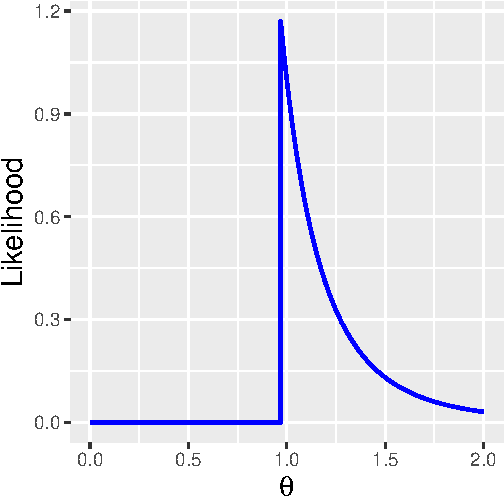
\includegraphics[keepaspectratio]{05-uniform_files/figure-latex/fig-uniflik-1.pdf}}

}

\caption{\label{fig-uniflik}The likelihood function given \(n=5\) data
drawn from a Uniform(0,\(\theta\)) distribution, with \(\theta = 1\). As
\(\theta\) cannot be smaller than the maximum observed value, the
likelihood is zero for \(\theta < X_{(n)}\); it is \(1/\theta^n\) for
\(\theta \geq X_{(n)}\). The maximum likelihood estimate is thus
\(X_{(n)}\) itself; as the likelihood function is not differentiable at
this point, the MLE cannot be found via the algorithm that we have used
previously.}

\end{figure}%

\smallskip\hrule

\begin{quote}
\textbf{Recall}: \emph{a sufficient statistic for a population parameter
\(\theta\) captures all information about \(\theta\) contained in a data
sample; no additional statistic will provide more information about
\(\theta\). Sufficient statistics are not unique: one-to-one functions
of sufficient statistics are themselves sufficient statistics.}
\end{quote}

\smallskip\hrule

Before we discuss sufficient statistics in the context of working with
domain-specifying parameters, it is useful to introduce the
\emph{indicator function}. This function takes on the value 1 if a
specified condition is met and 0 otherwise. For instance, \[
\mathbb{I}_{x_i \in [0,1]} = \left\{ \begin{array}{cl} 1 & x_i \in [0,1] \\ 0 & \mbox{otherwise} \end{array} \right. \,.
\] One use for the indicator function is to, well, \emph{indicate} the
domain of a pmf or pdf. For instance, we can write \[
f_X(x) = \left\{ \begin{array}{ll} e^{-x} & x \geq 0 \\ 0 & \mbox{otherwise} \end{array} \right.
\] to express that the exponential distribution with rate \(\theta = 1\)
is defined within the domain \(x \in [0,\infty)\), or, equivalently, we
can write \[
f_X(x) = e^{-x} \mathbb{I}_{x \in [0,\infty)} \,.
\] The latter form expresses the same information in a more condensed
fashion.

So\ldots why would we use indicator functions now?

Let's suppose we sample \(n\) iid data \(\{X_1,\ldots,X_n\}\) from a
uniform distribution with lower bound 0 and upper bound \(\theta\), and
our goal is to define a sufficient statistic for \(\theta\). Let's work
with the factorization criterion: \[
\mathcal{L}(\theta \vert \mathbf{x}) = g(\mathbf{x},\theta) \cdot h(\mathbf{x}) \,.
\] The likelihood is \[
\mathcal{L}(\theta \vert \mathbf{x}) = \prod_{i=1}^n f_X(x_i \vert \theta) = \prod_{i=1}^n \frac{1}{\theta} = \frac{1}{\theta^n} \,.
\] OK\ldots no\ldots wait: there are no data in this expression, so we
cannot (yet) read off a sufficient statistic for \(\theta\). Let's
re-express the pdf as \[
f_X(x) = \frac{1}{\theta} \mathbb{I}_{x \in [0,\theta]}
\] and rewrite the likelihood as \[
\mathcal{L}(\theta \vert \mathbf{x}) = \prod_{i=1}^n f_X(x_i \vert \theta) = \frac{1}{\theta^n} \prod_{i=1}^n \mathbb{I}_{x_i \in [0,\theta]} \,.
\] The product of indicator functions will equal 1 if and only if
\emph{all} data lie in the domain \(x \in [0,\theta]\). This is
equivalent to saying that \(\theta \geq X_{(n)}\), the order statistic
representing the maximum observed datum. Thus \(X_{(n)}\) is a
sufficient statistic for \(\theta\): we know \(\theta\) is greater than
this statistic's value, and none of the data aside from \(X_{(n)}\)
provide additional information about \(\theta\).

The upshot: when \(\theta\) is a domain-specifying parameter, a
sufficient statistic for \(\theta\) will be an order statistic (or any
one-to-one function of that order statistic).

When we first introduced the factorization criterion and sufficient
statistics in Section~\ref{sec-chap3point}, we did it so that ultimately
we could write down the minimum variance unbiased estimator (or MVUE).

\smallskip\hrule

\begin{quote}
\textbf{Recall}: \emph{the bias of an estimator is the difference
between the average value of the estimates it generates and the true
parameter value. If \(E[\hat{\theta}-\theta] = 0\), then the estimator
\(\hat{\theta}\) is said to be unbiased.}
\end{quote}

\smallskip\hrule

\begin{quote}
\textbf{Recall}: \emph{deriving the minimum variance unbiased estimator
involves two steps:}
\end{quote}

\begin{quote}
\begin{enumerate}
\def\labelenumi{\arabic{enumi}.}
\tightlist
\item
  \emph{factorizing the likelihood function to uncover a sufficient
  statistic \(U\) (that we assume is both minimal and complete); and}
\item
  \emph{finding a function \(h(U)\) such that \(E[h(U)] = \theta\).}
\end{enumerate}
\end{quote}

\smallskip\hrule

For instance, if \(\{X_1,\ldots,X_n\}\) are iid data sampled according
to a Uniform(\(0,\theta\)) distribution, can we define an MVUE for
\(\theta\)? The answer is yes\ldots as we will show in an example below.

(For completeness, we should mention that the method of moments
estimator for \(\theta\) can \emph{never} be a sufficient statistic,
since MoM estimators are not constructed from order statistics.)

\subsection{Examples}\label{examples-45}

\subsubsection{Uniform Domain Parameter:
MLE}\label{uniform-domain-parameter-mle}

\begin{quote}
Let \(\{X_1,\ldots,X_n\}\) be \(n\) iid data sampled according to a
Uniform(\(0,\theta\)) distribution. As shown above, the MLE for
\(\theta\) is \(X_{(n)}\), the maximum observed datum. The properties of
estimators that we have examined thus far include the bias (are our
estimates offset from the truth, on average?), the variance (over how
large a range do our estimates vary?), etc. Let's look at these
properties here.
\end{quote}

\smallskip\hrule

\begin{quote}
\textbf{Recall}: \emph{the maximum of \(n\) iid random variables sampled
from a pdf \(f_X(x)\) has a sampling distribution given by} \[
f_{(n)}(x) = n f_X(x) [ F_X(x) ]^{n-1} \,,
\] \emph{where \(F_X(x)\) is the associated cdf.}
\end{quote}

\smallskip\hrule

\begin{quote}
For the Uniform(\(0,\theta\)) distribution, \[
f_X(x) = \frac{1}{\theta} ~~\mbox{and}~~ F_X(x) = \int_0^x f_Y(y) dy = \int_0^x \frac{1}{\theta} dy = \frac{x}{\theta} \,,
\] so \[
f_{(n)}(x) = n \frac{1}{\theta} \left[ \frac{x}{\theta} \right]^{n-1} = n \frac{x^{n-1}}{\theta^n} \,.
\] The expected value of \(X_{(n)}\) is thus \[
E[X_{(n)}] = \int_0^\theta x n \frac{x^{n-1}}{\theta^n} dx = \left. \frac{n}{(n+1)\theta^n} x^{n+1} \right|_0^\theta = \frac{n}{n+1} \theta \,,
\] and the bias of the MLE for \(\theta\) is thus \[
B[\hat{\theta}_{MLE}] = E[\hat{\theta}_{MLE}] - \theta = \frac{n}{n+1}\theta - \theta = -\frac{1}{n+1}\theta \,.
\] The MLE is biased, but as we expect it is at least asymptotically
unbiased, as the bias goes to zero as \(n \rightarrow \infty\).
\end{quote}

\smallskip\hrule

\begin{quote}
\textbf{Recall}: \emph{an estimator is consistent if its mean-squared
error, \(B[\hat{\theta}]^2 + V[\hat{\theta}]\), goes to zero as the
sample size \(n\) goes to infinity.}
\end{quote}

\smallskip\hrule

\begin{quote}
The variance of the MLE is \[
V[\hat{\theta}_{MLE}] = E[\hat{\theta}_{MLE}^2] - \left(E[\hat{\theta}_{MLE}\right)^2 = E[X_{(n)}^2] - (E[X_{(n)}])^2 \,.
\] To derive the variance, we need to determine \(E[X_{(n)}^2]\): \[
E[X_{(n)}^2] = \int_0^\theta x^2 n \frac{x^{n-1}}{\theta^n} dx = \left. \frac{n}{(n+2)\theta^n} x^{n+2} \right|_0^\theta = \frac{n}{n+2} \theta^2 \,.
\] So now we can write down that \[
V[\hat{\theta}_{MLE}] = \frac{n}{n+2}\theta^2 - \left( \frac{n}{n+1}\theta\right)^2 = \frac{n}{(n+2)(n+1)^2}\theta^2 \rightarrow \frac{\theta^2}{n^2} ~~\mbox{as}~~ n \rightarrow \infty\,.
\] We observe that because the variance goes to zero as
\(n \rightarrow \infty\), the mean-squared error does as well\ldots and
thus the MLE for \(\theta\) is a consistent estimator.
\end{quote}

\subsubsection{Pareto Domain Parameter:
MLE}\label{pareto-domain-parameter-mle}

\begin{quote}
Recall that the Pareto distribution has the probability density function
\[
f_X(x) = \frac{a b^a}{x^{a+1}} \,,
\] where \(a > 0\) and \(x \in [b,\infty)\). Because \(b\) is a
domain-specifying parameter, we find the MLE not via differentiation but
rather by identifying that the likelihood is maximized when \(b\) is
exactly equal to \(X_{(1)}\), i.e., \(\hat{b}_{MLE} = X_{(1)}\). See
Figure Figure~\ref{fig-parlik}.
\end{quote}

\begin{figure}

\centering{

\pandocbounded{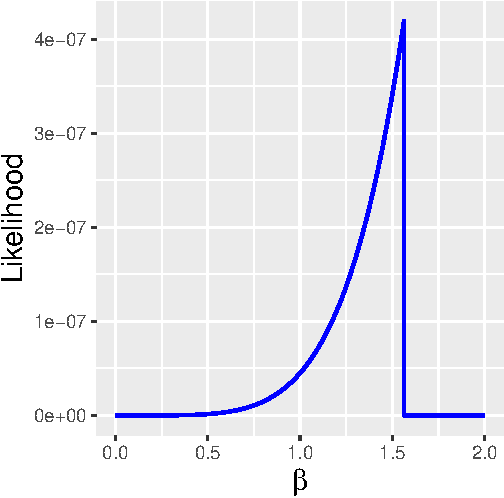
\includegraphics[keepaspectratio]{05-uniform_files/figure-latex/fig-parlik-1.pdf}}

}

\caption{\label{fig-parlik}The likelihood function given \(n=5\) data
drawn from a Pareto(1,\(b\)) distribution, with \(b = 1\). As \(b\)
cannot be larger than the minimum observed value, the likelihood is zero
for \(b \geq X_{(1)}\); it is \(\theta^n(1/\prod_{i=1}^n x_i)^2\) for
\(b < X_{(n)}\). The maximum likelihood estimate is thus \(X_{(1)}\)
itself; as the likelihood function is not differentiable at this point,
the MLE cannot be found via the algorithm we have used previously.}

\end{figure}%

\subsubsection{Uniform Domain Parameter:
MVUE}\label{uniform-domain-parameter-mvue}

\begin{quote}
Above, we determined that if we sample \(n\) iid data according to a
Uniform\((0,\theta)\) distribution, a sufficient statistic for
\(\theta\) is \(X_{(n)}\) and the expected value of \(X_{(n)}\) is
\(n\theta/(n+1)\). Given this information, it is trivial to rearrange
terms and to write down the MVUE for \(\theta\): \[
E\left[\frac{n+1}{n}X_{(n)}\right] = \theta ~~~ \Rightarrow ~~~ \hat{\theta}_{MVUE} = \frac{n+1}{n}X_{(n)} \,.
\] The variance of \(\hat{\theta}_{MVUE}\) is \begin{align*}
V[\hat{\theta}_{MVUE}] &= E\left[\left(\hat{\theta}_{MVUE}\right)^2\right] - \left( E\left[ \hat{\theta}_{MVUE} \right] \right)^2 \\
&= \frac{(n+1)^2}{n^2} \left( E[X_{(n)}^2] - (E[X_{(n)}])^2 \right) \,,
\end{align*} where \[
E[X_{(n)}^2] = \int_0^\theta x^2 n \frac{x^{n-1}}{\theta^n} dx = \left. \frac{n}{(n+2)\theta^n} x^{n+2} \right|_0^\theta = \frac{n}{n+2} \theta^2 \,.
\] Thus \begin{align*}
V[\hat{\theta}_{MVUE}] &= \frac{(n+1)^2}{n^2} \left( \frac{n}{n+2} \theta^2 - \frac{n^2}{(n+1)^2} \theta^2 \right) \\
&= \frac{(n+1)^2}{n^2} \left( \frac{n(n+1)^2 - n^2(n+2)}{(n+2)(n+1)^2} \theta^2 \right) \\
&= \frac{(n+1)^2}{n^2} \left( \frac{n}{(n+2)(n+1)^2} \theta^2 \right) \\
&= \frac{1}{n(n+2)} \theta^2 \rightarrow \frac{\theta^2}{n^2} ~~\mbox{as}~~ n \rightarrow \infty \,.
\end{align*} We observe that since the variance goes to zero as
\(n \rightarrow \infty\), the MVUE is a consistent estimator\ldots but
does it achieve the Cramer-Rao Lower Bound (CRLB), the theoretical lower
bound on the variance of unbiased estimators?
\end{quote}

\smallskip\hrule

\begin{quote}
\textbf{Recall}: \emph{the Cramer-Rao Lower Bound (or CRLB) is the lower
bound on the variance of any unbiased estimator. If an unbiased
estimator achieves the CRLB, it is the MVUE\ldots but it can be the case
that the MVUE does not achieve the CRLB. For a discrete distribution,
the CRLB is given by} \[
V_{\mathrm{CRLB}}[\hat{\theta}] = -\left(nE\left[\frac{d^2}{d\theta^2} \log p_X(X \vert p) \right]\right)^{-1} = \frac{1}{nI(\theta)}
\] \emph{where \(I(\theta)\) is the Fisher information:} \[
I(\theta) = -E\left[ \frac{\partial^2}{\partial \theta^2} \log f_X(x \vert \theta) \right] \,.
\]
\end{quote}

\smallskip\hrule

\begin{quote}
It turns out that not only does it achieve the lower bound (which one
can show equals \(\theta^2/n\)), but it even surpasses that bound, as \[
\frac{1}{n(n+2)} \theta^2 < \frac{1}{n} \theta^2 \,.
\] Ultimately, we need not worry about this seemingly worrisome result,
because one of the so-called regularity conditions that must hold for
the bound calculation to be valid is that the log-likelihood is
differentiable everywhere within a distribution's domain\ldots but this
condition does \emph{not} hold when we are working with
domain-specifying parameters.
\end{quote}

\begin{quote}
The variance of the MLE is similar to, but not exactly the same as, the
variance for the MVUE, although the two variances converge to the same
value in as \(n \rightarrow \infty\).
\end{quote}

\subsubsection{Pareto Domain Parameter:
MVUE}\label{pareto-domain-parameter-mvue}

\begin{quote}
The Pareto probability density function is \[
f_X(x) = \frac{a b^a}{x^{a+1}} \,,
\] where \(a > 0\) and \(x \in [b,\infty)\). Let's assume \(a\) is
fixed. A sufficient statistic for \(b\), found via likelihood
factorization, is \[
\mathcal{L}(b \vert \mathbf{x}) = \prod_{i=1}^n f_X(x_i) = \underbrace{b^{na}}_{g(\mathbf{x},b)} \cdot \underbrace{\frac{a^n}{(\prod_{i=1}^n x_i)^{a+1}}}_{h(\mathbf{x})} \,.
\] Wait\ldots again, as is the case for the uniform distribution, no
data appear in the expression \(g(\cdot)\). So we would go back and
introduce an indicator function into the pdf; it should be clear that
when we do so, \(g(\mathbf{x},b)\) changes to \[
g(\mathbf{x},b) = b^{na} \prod_{i=1}^n \mathbb{I}_{x_i \in [b,\infty)}
\] and thus that because all data have to be larger than \(b\), a
sufficient statistic will be the minimum observed datum, \(X_{(1)}\).
\end{quote}

\begin{quote}
To go from here to finding the MVUE, we need to derive a number of
quantities:
\end{quote}

\begin{quote}
\begin{itemize}
\tightlist
\item
  the cumulative distribution function for a Pareto distribution;
\item
  the probability density function for the smallest-valued of \(n\)
  Pareto random variables; and
\item
  the expected value of this smallest-valued random variable.
\end{itemize}
\end{quote}

\begin{quote}
Let's do each in turn.
\end{quote}

\begin{quote}
As for the cdf: \begin{align*}
F_X(x) = \int_b^x \frac{a b^a}{y^{a+1}} dy &= a b^a \int y^{-a-1} dy = a b^a \left. \frac{1}{-a} y^{-a} \right|_b^x \\
&= b^a \left. y^{-a} \right|_x^b = b^a \left( b^{-a} - x^{-a} \right) = 1 - \left(\frac{b}{x}\right)^a \,.
\end{align*} The pdf for the smallest-valued of \(n\) iid Pareto data is
given by \begin{align*}
f_{(1)}(x) &= n f_X(x) \left[ 1 - F_X(x) \right]^{n-1} \\
&= n \frac{a b^a}{x^{a+1}} \left[ 1 - \left( 1 - \left[\frac{b}{x}\right]^a \right) \right]^{n-1} \\
&= n \frac{a b^a}{x^{a+1}} \left(\frac{b}{x}\right)^{na-a} \\
&= n \frac{a b^{na}}{x^{na+1}} \,.
\end{align*} Last, the expected value of this datum is \begin{align*}
E[X_{(1)}] &= \int_b^\infty n x \frac{a b^{na}}{x^{na+1}} = n a b^{na} \int_b^\infty x^{-na} dx \\
&= n a b^{na} \frac{1}{-na+1} \left. x^{-na+1} \right|_b^\infty \\
&= n a b^{na} \frac{1}{-na+1} \left( 0 - b^{-na+1} \right) \\
&= \frac{n a b}{na-1} \,.
\end{align*} Hence we see that \[
E\left[\frac{na-1}{na} X_{(1)}\right] = b
\] and that \[
\hat{b}_{\mathrm{MVUE}} = \frac{na-1}{na} X_{(1)} \,.
\]
\end{quote}

\section{Confidence Intervals}\label{sec-chap5confidence}

What to take away from this section:

\begin{itemize}
\item
  Interval estimates for distribution bounds generated using sufficient
  statistics (i.e., order statistics) behave ``properly'' in that they
  do not overlap the value of the statistic itself.
\item
  Constructing one-sided confidence intervals is superior to
  constructing two-sided confidence intervals when we wish to make
  inferences about domain-specifying parameters.
\end{itemize}

For previous material on confidence intervals, see
Section~\ref{sec-chap4confidence}.

\smallskip\hrule

\begin{quote}
\textbf{Recall:} \emph{a confidence interval is a random interval
\([\hat{\theta}_L,\hat{\theta}_U]\) that overlaps (or covers) the true
value \(\theta\) with probability} \[
P\left( \hat{\theta}_L \leq \theta \leq \hat{\theta}_U \right) = 1 - \alpha \,,
\] \emph{where \(1 - \alpha\) is the confidence coefficient. Note that
this is a long-term probabilistic statement that is not to be applied to
any one numerically evaluated interval: an evaluated interval either
overlaps the true value, or it does not (and thus we cannot say there is
a \(100(1-\alpha)\)-percent chance that \(\theta\) lies within the
interval). We determine \(\hat{\theta}\) by solving the following
equation:} \[
F_Y(y_{\mathrm{obs}} \vert \theta) - q = 0 \,,
\] \emph{where \(F_Y(\cdot)\) is the cumulative distribution function
for the statistic \(Y\), \(y_{\mathrm{obs}}\) is the observed value of
the statistic, and \(q\) is an appropriate quantile value that is
determined using the confidence interval reference table introduced in
Section~\ref{sec-chap1confref}.}
\end{quote}

\smallskip\hrule

Our coverage, so to speak, of confidence intervals in very nearly
complete and there is little for us to add to the discussion
now\ldots{}\emph{except}\ldots{}

In the first example below, we demonstrate that one of the quirks of
statistical inference with domain-specifying parameters is that,
regardless of any research questions we are trying to answer when we
analyze data, constructing \(100(1-\alpha)\)-percent one-sided intervals
is superior to constructing \(100(1-\alpha)\)-percent two-sided
intervals. And in the second example, we circle back around to a point
made back in Section~\ref{sec-chap1confidence}: \(1-\alpha\) is
technically the infimum, or minimum value, of
\(P\left( \hat{\theta}_L \leq \theta \leq \hat{\theta}_U \right)\), even
though throughout the book we have treated it as a user-specified
constant. How might we define confidence intervals such that their
coverage is technically zero?

\subsection{Examples}\label{examples-46}

\subsubsection{Uniform Domain Parameter: Interval
Estimation}\label{uniform-domain-parameter-interval-estimation}

\begin{quote}
Recall that when we sample \(n\) iid data according to a
Uniform(\(0,\theta\)) distribution, a sufficient statistic is
\(Y = X_{(n)}\), which has probability density function \[
f_Y(y) = f_{(n)}(x) = n \frac{x^{n-1}}{\theta^n} \,,
\] cumulative distribution function \[
F_Y(y) = F_{(n)}(x) = (x/\theta)^n \,,
\] and expected value \[
E[Y] = E[X_{(n)}] = \frac{n}{n+1} \theta \,.
\] Given that \(E[Y]\) increases with \(\theta\), we know that we will
be working with quantities on the ``yes'' line of the confidence
interval reference table.
\end{quote}

\begin{quote}
To find the lower and upper bounds on \(\theta\), respectively, for a
two-sided interval, we solve for \(\theta\) in the expressions
\begin{align*}
\left(\frac{X_{(n)}}{\theta}\right)^n - \left(1 - \frac{\alpha}{2}\right) &= 0 ~~~ \mbox{(lower)} \\
\left(\frac{X_{(n)}}{\theta}\right)^n - \frac{\alpha}{2} &= 0 ~~~ \mbox{(upper)} \,,
\end{align*} and we find that \[
\hat{\theta}_L = \frac{X_{(n)}}{(1-\alpha/2)^{1/n}} ~~\mbox{and}~~ \hat{\theta}_U = \frac{X_{(n)}}{(\alpha/2)^{1/n}} \,.
\]
\end{quote}

\begin{quote}
In Figure~\ref{fig-unifci}, we display 10 separate 90 percent confidence
intervals generated using data sampled according to a Uniform(0,1)
distribution. In this figure, the maximum observed values for each
dataset are shown as red crosses, while the intervals are displayed as
blue lines. We immediately see one of the quirks associated with
domain-specifying parameters: the observed data do not lie within the
intervals (as they have previously) but rather outside of them. This is
good: no observed value of \(X_{(n)}\) should be larger than the derived
lower bound! (Otherwise it would be impossible to observe that value, if
indeed the derived lower bound is the true value.)
\end{quote}

\begin{figure}

\centering{

\pandocbounded{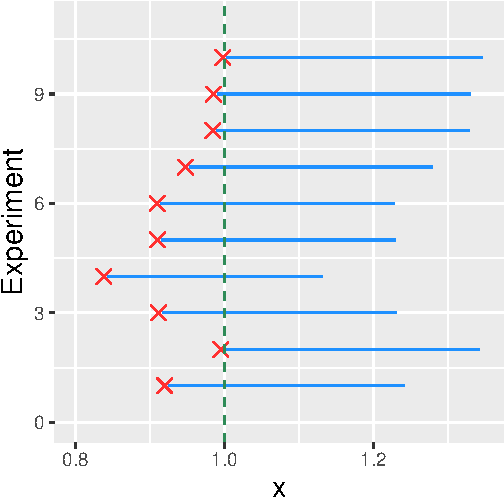
\includegraphics[keepaspectratio]{05-uniform_files/figure-latex/fig-unifci-1.pdf}}

}

\caption{\label{fig-unifci}Ten 90 percent confidence intervals,
generated using data from 10 separate datasets of size \(n = 10\)
sampled according to a Uniform(\(0,\theta\)) distribution. (Here,
\(\theta = 1\).) The observed statistic values \(X_{(n)}\) are shown as
red crosses; in each case, the values lie outside the derived
intervals.}

\end{figure}%

\begin{quote}
Now, let's take one of the datasets used to construct
Figure~\ref{fig-unifci}, and look at its associated confidence interval:
\end{quote}

\begin{Shaded}
\begin{Highlighting}[]
\FunctionTok{round}\NormalTok{(X, }\DecValTok{3}\NormalTok{)}
\end{Highlighting}
\end{Shaded}

\begin{verbatim}
 [1] 0.335 0.494 0.613 0.672 0.687 0.764 0.797 0.842 0.888 0.920
\end{verbatim}

\begin{Shaded}
\begin{Highlighting}[]
\FunctionTok{cat}\NormalTok{(}\StringTok{"The maximum value is                      "}\NormalTok{, }\FunctionTok{round}\NormalTok{(}\FunctionTok{max}\NormalTok{(X), }\DecValTok{3}\NormalTok{), }\StringTok{"}\SpecialCharTok{\textbackslash{}n}\StringTok{"}\NormalTok{)}
\end{Highlighting}
\end{Shaded}

\begin{verbatim}
The maximum value is                       0.92 
\end{verbatim}

\begin{Shaded}
\begin{Highlighting}[]
\FunctionTok{cat}\NormalTok{(}\StringTok{"The two{-}sided 90\% confidence interval is ["}\NormalTok{, }\FunctionTok{round}\NormalTok{(hat.theta.L, }\DecValTok{3}\NormalTok{), }\StringTok{","}\NormalTok{,}
     \FunctionTok{round}\NormalTok{(hat.theta.U, }\DecValTok{3}\NormalTok{), }\StringTok{"]}\SpecialCharTok{\textbackslash{}n}\StringTok{"}\NormalTok{)}
\end{Highlighting}
\end{Shaded}

\begin{verbatim}
The two-sided 90% confidence interval is [ 0.925 , 1.242 ]
\end{verbatim}

\begin{quote}
What do we observe? On one side of our two-sided interval, there is a
small gap between the value of the maximum datum (0.920) and the value
of \(\hat{\theta}_L\) (0.925). We also observe the width of the interval
to be \(1.242 - 0.925 = 0.317\).
\end{quote}

\begin{quote}
What would happen if we were to construct a 90\% one-sided upper bound
on \(\theta\) instead? The lower bound would effectively shift very
little, from 0.925 to 0.920, while the upper bound would shift from
1.242 to \[
\hat{\theta}_U = \frac{X_{(n)}}{\alpha^{1/n}} = \frac{0.920}{(0.1)^{1/10}} = 1.158 \,.
\] The interval width changes from 0.317 to 0.238, a decrease of nearly
25\%! In the end, when attempting to quantify our uncertainty about the
value of \(\theta\), we become slightly more uncertain in one direction
(adding the range \([0.920,0.925)\) to our interval) but substantially
less uncertain in the other (removing the range \((1.158,1.242]\) from
our interval). We thus find that \emph{one-sided confidence intervals
are superior to two-sided ones when we are trying to infer
domain-specifying parameters}.
\end{quote}

\subsubsection{Uniform Domain Parameter: Confidence
Coefficient}\label{uniform-domain-parameter-confidence-coefficient}

\begin{quote}
A confidence interval is a random interval
\([\hat{\theta}_L,\hat{\theta}_U]\) that covers the true value
\(\theta\) with probability \[
P\left( \hat{\theta}_L \leq \theta \leq \hat{\theta}_U \right) = 1 - \alpha \,,
\] where \(1 - \alpha\) is the confidence coefficient. In
Section~\ref{sec-chap1confidence}, we make the point that technically,
the confidence coefficient is the infimum, or minimum value, of
\(P(\hat{\theta}_L \leq \theta \leq \hat{\theta}_U)\). What does this
actually mean in practice?
\end{quote}

\begin{quote}
In the example above, we show that the interval estimate with confidence
coefficient \(1-\alpha\) for the uniform upper bound \(\theta\) has the
form \([aX_{(n)},bX_{(n)}]\). Can we also define an appropriate interval
estimator if, for instance, it has the form
\([X_{(n)} + a,X_{(n)} + b]\)? The short answer is no\ldots because the
confidence coefficient will be \emph{zero}! To see why, let's work
directly with the probability statement that defines the confidence
coefficient: \begin{align*}
P(X_{(n)} + a \leq \theta \leq X_{(n)} + b) &= P(\theta - b \leq X_{(n)} \leq \theta - a)\\
&= P(X_{(n)} \leq \theta - a) - P(X_{(n)} \leq \theta - b)\\
&= F_{(n)}(\theta-a) - F_{(n)}(\theta-b)\\
&= \left(\frac{\theta-a}{\theta}\right)^2 - \left(\frac{\theta-b}{\theta}\right)^2\\
&= \left(1-\frac{a}{\theta}\right)^2 - \left(1-\frac{b}{\theta}\right)^2 \,.
\end{align*} The key to interpreting the last line above is that
\(\theta\) is \emph{unknown} (otherwise, why would we be constructing a
confidence interval for it in the first place?), and thus can take on
any allowable value. For an interval of the form
\([aX_{(n)},bX_{(n)}]\), \(\theta\) does not appear, and thus the
confidence coefficient is the user-set constant \(1 - \alpha\). Here,
however, \[
\lim_{\theta \to \infty} P(X_{(n)} + a \leq \theta \leq X_{(n)} + b) = 0 \,,
\] and thus the confidence coefficient (or the proportion of computed
intervals that overlap the true value \(\theta\)) goes to zero. Thus an
interval estimator of the form \([aX_{(n)},bX_{(n)}]\) is a better one
than one of the form \([X_{(n)} + a,X_{(n)} + b]\).
\end{quote}

\begin{quote}
The upshot: one cannot just write down any interval and assume that it
comes with a guarantee of non-zero coverage! It turns out that by
working with the sampling distributions of statistics, useful interval
estimators are naturally defined for us.
\end{quote}

\subsubsection{Pareto Domain Parameter: Interval
Estimation}\label{pareto-domain-parameter-interval-estimation}

\begin{quote}
As was mentioned earlier in Section~\ref{sec-chap5linear}, a
moment-generating function does not exist for the Pareto distribution.
Thus if we sample \(n > 1\) iid data according to this distribution
(with fixed parameter \(a\)), we cannot begin to analytically identify
the sampling distribution for, e.g., \(Y = \sum_{i=1}^n X_i\)\ldots so
we would have to utilize a simulation framework to construct intervals
with this statistic. But it turns out that this doesn't actually matter
to us, as we have since found out that a sufficient statistic for the
Pareto \(b\) parameter is \(X_{(1)}\), and we certainly do know the cdf
of the sampling distribution for that: \begin{align*}
F_{(1)}(x) &= \int_b^x \frac{n a b^{na}}{y^{na+1}} dy = n a b^{na} \int_b^x y^{-na-1} dy \\
&= n a b^{na} \frac{1}{-na} \left. y^{-na} \right|_b^x = - b^{na} \left( x^{-na} - b^{-na} \right) \\
&= 1 - \left(\frac{b}{x}\right)^{na} \,.
\end{align*} If we solve the general equation
\(F_Y(y_{\mathrm{obs}} \vert \theta) - q = 0\), we find that \[
\hat{b}(q) = x_{(1),\mathrm{obs}} (1 - q)^{1/na} \,.
\]
\end{quote}

\begin{quote}
But, for review purposes, let's say we really want to utilize the sample
mean as our interval-constructing statistic. (We shouldn't, because it
is not a sufficient statistic for \(b\), but we are headstrong and are
going to plow ahead.) Below we show a simulation framework for
estimating a 95\% lower bound for \(b\), given that \(a = 3\) and
\(n = 8\). Note that the expected value of \(\bar{X}\) increases with
\(b\), as the reader can verify, so \(q = 1-\alpha = 0.95\).
\end{quote}

\begin{Shaded}
\begin{Highlighting}[]
\CommentTok{\# generate data}
\FunctionTok{set.seed}\NormalTok{(}\DecValTok{236}\NormalTok{)}
\NormalTok{num.sim }\OtherTok{\textless{}{-}} \DecValTok{100000}
\NormalTok{n       }\OtherTok{\textless{}{-}} \DecValTok{8}
\NormalTok{a       }\OtherTok{\textless{}{-}} \DecValTok{3}
\NormalTok{b       }\OtherTok{\textless{}{-}} \FloatTok{1.5}
\NormalTok{X.obs   }\OtherTok{\textless{}{-}}\NormalTok{ extraDistr}\SpecialCharTok{::}\FunctionTok{rpareto}\NormalTok{(n, }\AttributeTok{a =}\NormalTok{ a, }\AttributeTok{b =}\NormalTok{ b) }\CommentTok{\# coded to avoid namespace conflict}
\NormalTok{y.obs   }\OtherTok{\textless{}{-}} \FunctionTok{mean}\NormalTok{(X.obs)}
\NormalTok{alpha   }\OtherTok{\textless{}{-}} \FloatTok{0.05}

\FunctionTok{min}\NormalTok{(X.obs)}
\end{Highlighting}
\end{Shaded}

\begin{verbatim}
[1] 1.582117
\end{verbatim}

\begin{Shaded}
\begin{Highlighting}[]
\CommentTok{\# the 95\% lower bound given X\_(1)}
\FunctionTok{round}\NormalTok{(}\FunctionTok{min}\NormalTok{(X.obs) }\SpecialCharTok{*}\NormalTok{ alpha}\SpecialCharTok{\^{}}\NormalTok{(}\DecValTok{1} \SpecialCharTok{/}\NormalTok{ (n }\SpecialCharTok{*}\NormalTok{ a)), }\DecValTok{3}\NormalTok{)}
\end{Highlighting}
\end{Shaded}

\begin{verbatim}
[1] 1.396
\end{verbatim}

\begin{Shaded}
\begin{Highlighting}[]
\CommentTok{\# the 95\% lower bound given X.bar}
\NormalTok{f }\OtherTok{\textless{}{-}} \ControlFlowTok{function}\NormalTok{(b, a, n, y.obs, q, }\AttributeTok{num.sim =} \DecValTok{1000000}\NormalTok{, }\AttributeTok{seed =} \DecValTok{236}\NormalTok{)}
\NormalTok{\{}
  \FunctionTok{set.seed}\NormalTok{(seed)}
\NormalTok{  X }\OtherTok{\textless{}{-}} \FunctionTok{matrix}\NormalTok{(extraDistr}\SpecialCharTok{::}\FunctionTok{rpareto}\NormalTok{(num.sim }\SpecialCharTok{*}\NormalTok{ n, }\AttributeTok{a =}\NormalTok{ a, }\AttributeTok{b =}\NormalTok{ b), }\AttributeTok{nrow =}\NormalTok{ num.sim)}
\NormalTok{  Y }\OtherTok{\textless{}{-}} \FunctionTok{rowMeans}\NormalTok{(X)}
  \FunctionTok{sum}\NormalTok{(Y }\SpecialCharTok{\textless{}=}\NormalTok{ y.obs) }\SpecialCharTok{/}\NormalTok{ num.sim }\SpecialCharTok{{-}}\NormalTok{ q}
\NormalTok{\}}

\FunctionTok{round}\NormalTok{(}\FunctionTok{uniroot}\NormalTok{(f, }\AttributeTok{interval =} \FunctionTok{c}\NormalTok{(}\FloatTok{0.001}\NormalTok{, }\DecValTok{1000}\NormalTok{), }\AttributeTok{a =}\NormalTok{ a, }\AttributeTok{n =}\NormalTok{ n,}
              \AttributeTok{y.obs =}\NormalTok{ y.obs, }\AttributeTok{q =} \DecValTok{1} \SpecialCharTok{{-}}\NormalTok{ alpha)}\SpecialCharTok{$}\NormalTok{root, }\DecValTok{3}\NormalTok{)}
\end{Highlighting}
\end{Shaded}

\begin{verbatim}
[1] 0.989
\end{verbatim}

\begin{quote}
The lower bound found given the sufficient statistic \(X_{(1)}\) is
1.396, while the lower bound found given \(\bar{X}\) is 0.989. This
result demonstrates that the utilization of sufficient statistics
results in superior inferences (meaning, here, smaller intervals).
\end{quote}

\begin{quote}
But let's take this example just a little farther: let's compute a 95\%
\emph{upper bound} while utilizing the sample mean. (We utilize the same
code as above, but we change \texttt{q\ =\ 1\ -\ alpha} to
\texttt{q\ =\ alpha} in the call to \texttt{uniroot()}.)
\end{quote}

\begin{Shaded}
\begin{Highlighting}[]
\CommentTok{\# the 95\% upper bound given X.bar}
\NormalTok{f }\OtherTok{\textless{}{-}} \ControlFlowTok{function}\NormalTok{(b, a, n, y.obs, q, }\AttributeTok{num.sim =} \DecValTok{1000000}\NormalTok{, }\AttributeTok{seed =} \DecValTok{236}\NormalTok{)}
\NormalTok{\{}
  \FunctionTok{set.seed}\NormalTok{(seed)}
\NormalTok{  X }\OtherTok{\textless{}{-}} \FunctionTok{matrix}\NormalTok{(extraDistr}\SpecialCharTok{::}\FunctionTok{rpareto}\NormalTok{(num.sim }\SpecialCharTok{*}\NormalTok{ n, }\AttributeTok{a =}\NormalTok{ a, }\AttributeTok{b =}\NormalTok{ b), }\AttributeTok{nrow =}\NormalTok{ num.sim)}
\NormalTok{  Y }\OtherTok{\textless{}{-}} \FunctionTok{rowMeans}\NormalTok{(X)}
  \FunctionTok{sum}\NormalTok{(Y }\SpecialCharTok{\textless{}=}\NormalTok{ y.obs) }\SpecialCharTok{/}\NormalTok{ num.sim }\SpecialCharTok{{-}}\NormalTok{ q}
\NormalTok{\}}

\FunctionTok{round}\NormalTok{(}\FunctionTok{uniroot}\NormalTok{(f, }\AttributeTok{interval =} \FunctionTok{c}\NormalTok{(}\FloatTok{0.001}\NormalTok{, }\DecValTok{1000}\NormalTok{), }\AttributeTok{a =}\NormalTok{ a, }\AttributeTok{n =}\NormalTok{ n,}
              \AttributeTok{y.obs =}\NormalTok{ y.obs, }\AttributeTok{q =}\NormalTok{ alpha)}\SpecialCharTok{$}\NormalTok{root, }\DecValTok{3}\NormalTok{)}
\end{Highlighting}
\end{Shaded}

\begin{verbatim}
[1] 1.666
\end{verbatim}

\begin{quote}
The upper bound is 1.666. We can immediately see that this is
problematic since the smallest value among our eight data is
\(x_{(1),{\mathrm{obs}}} = 1.582\): we should not infer an upper bound
on \(b\) that exceeds any of the data values we observe!
\end{quote}

\section{Hypothesis Testing}\label{sec-chap5hypothesis}

What to take away from this section:

\begin{itemize}
\item
  When conducting hypothesis tests concerning distribution bounds, one
  can define two-tail tests, but from the perspective of power, it is
  preferable to define one-tail tests only.
\item
  When computing the test power for a hypothesis test, one must take
  into account the two ways in which one can reject the null hypothesis;
  for instance, if \(H_o : \theta = \theta_o\) is an upper distribution
  bound, and we wish to compute the test power given
  \(\theta > \theta_o\), then we would reject the null if \(X_{(n)}\)
  fall into the rejection region defined under the null \emph{and} if
  \(X_{(n)} > \theta_o\).
\end{itemize}

For previous material on hypothesis testing, see
Section~\ref{sec-chap4hypothesis}.

\smallskip\hrule

\begin{quote}
\textbf{Recall}: \emph{a hypothesis test is a framework to make an
inference about the value of a population parameter \(\theta\). The null
hypothesis \(H_o\) is that \(\theta = \theta_o\), while possible
alternatives \(H_a\) are \(\theta \neq \theta_o\) (two-tail test),
\(\theta > \theta_o\) (upper-tail test), and \(\theta < \theta_o\)
(lower-tail test). For, e.g., a one-tail test, we reject the null
hypothesis if the observed test statistic \(y_{\mathrm{obs}}\) falls
outside the bound given by \(y_{RR}\), which is a solution to the
equation} \[
F_Y(y_{RR} \vert \theta_o) - q = 0 \,,
\] \emph{where \(F_Y(\cdot)\) is the cumulative distribution function
for the statistic \(Y\) and \(q\) is an appropriate quantile value that
is a function of the adopted Type I error rate \(\alpha\). Note that the
hypothesis test framework only allows us to make a decision about a null
hypothesis; nothing is proven.}
\end{quote}

\smallskip\hrule

Let's suppose that we sample \(n\) iid data according to a
Uniform(0,\(\theta\)) and that we wish to construct a two-tail
hypothesis test using the sufficient statistic \(Y = X_{(n)}\). From
examples above, we know that \(F_Y(y) = (x/\theta)^n\) and that we are
working on the ``yes'' line of the reference table\ldots so the
rejection-region boundaries are given by \begin{align*}
F_{(n)}(x_{\mathrm{RR,lo}} \vert \theta_o) - \frac{\alpha}{2} = 0 ~~~ &\Rightarrow ~~~ x_{\mathrm{RR,lo}} = \theta_o \left( \frac{\alpha}{2} \right)^{1/n} \\
F_{(n)}(x_{\mathrm{RR,hi}} \vert \theta_o) - \left(1 - \frac{\alpha}{2}\right) = 0 ~~~ &\Rightarrow ~~~ x_{\mathrm{RR,hi}} = \theta_o \left( 1 - \frac{\alpha}{2} \right)^{1/n} \,.
\end{align*} If \(\theta > x_{\mathrm{RR,hi}}\), the power of the test
is \begin{align*}
power(\theta) &= F_{(n)}(x_{\mathrm{RR,lo}} \vert \theta) + \left[ 1 - F_{(n)}(x_{\mathrm{RR,hi}} \vert \theta) \right] \\ 
\Rightarrow ~~~ power(\theta) &= \left(\frac{\theta_o}{\theta}\right)^n \frac{\alpha}{2} + 1 - \left(\frac{\theta_o}{\theta}\right)^n \left(1-\frac{\alpha}{2}\right) = 1 - \left(\frac{\theta_o}{\theta}\right)^n(1-\alpha) \,.
\end{align*} So far, so good. But what would happen if we were to define
a lower-tail test instead? The rejection-region boundary would be given
by \begin{align*}
F_{(n)}(x_{\mathrm{RR}} \vert \theta_o) - \alpha = 0 ~~~ \Rightarrow ~~~ x_{\mathrm{RR}} = \theta_o \alpha^{1/n} \,.
\end{align*} Also so far, so good. But in a power calculation, we would
need to take into account that if \(\theta > \theta_o\), there are there
are \emph{two possible ways to reject the null}\ldots by observing

\begin{enumerate}
\def\labelenumi{\arabic{enumi}.}
\tightlist
\item
  \(x_{(n),\mathrm{obs}} < y_{\mathrm{RR}}\) (``traditional
  rejection''), or
\item
  \(x_{(n),\mathrm{obs}} > \theta_o\) (``trivial rejection'').
\end{enumerate}

We dub the second possibility ``trivial rejection'' since if the null is
correct, it is impossible to sample a datum with a value larger than
\(\theta_o\), and thus there is no need to computationally derive a
boundary for this part of the rejection region.

So, despite the fact that we are intending to define a one-tail test, we
have, in the context of power calculations, effectively defined a
two-tail test! The question then arises: from the point of view of test
power, which of these defined tests is better for us to use? Let's
examine the difference in power between the one-tail and two-tail tests
in three different regimes: \(\theta \leq x_{\mathrm{RR,hi}}\),
\(x_{\mathrm{RR,hi}} < \theta \leq \theta_o\), and
\(\theta > \theta_o\).

\begin{enumerate}
\def\labelenumi{\arabic{enumi}.}
\tightlist
\item
  If \(\theta \leq x_{\mathrm{RR,hi}}\), then the difference in power is
  \begin{align*}
  power_1(\theta) - power_2(\theta) &= F_{(n)}(x_{\mathrm{RR}} \vert \theta) - F_{(n)}(x_{\mathrm{RR,lo}} \vert \theta) \\
  &= \left(\frac{x_{\mathrm{RR}}}{\theta}\right)^n - \left(\frac{x_{\mathrm{RR,hi}}}{\theta}\right)^n \\
  &= \left(\frac{\theta_o}{\theta}\right)^n \left(\alpha - \frac{\alpha}{2}\right)\\
  &= \frac{\alpha}{2}\left(\frac{\theta_o}{\theta}\right)^n > 0 \,.
  \end{align*} In this regime, the one-tail test is more powerful.
\item
  If \(x_{\mathrm{RR,hi}} < \theta \leq \theta_o\), then the difference
  in power is \begin{align*}
  power_1(\theta) - power_2(\theta) &= F_{(n)}(x_{\mathrm{RR}} \vert \theta) - \left[ F_{(n)}(x_{\mathrm{RR,lo}} \vert \theta) + 1 - F_{(n)}(x_{\mathrm{RR,hi}} \vert \theta) \right] \\
  &= \left(\frac{\theta_o}{\theta}\right)^n \alpha - \left[ \left(\frac{\theta_o}{\theta}\right)^n \frac{\alpha}{2} + 1 - \left(\frac{\theta_o}{\theta}\right)^n \left(1 - \frac{\alpha}{2}\right) \right] \\
  &= \left(\frac{\theta_o}{\theta}\right)^n - 1 \geq 0 \,.
  \end{align*} In this regime, the one-tail test is more powerful,
  unless \(\theta = \theta_o\), where both power values are \(\alpha\).
\item
  If \(\theta > \theta_o\), then the difference in power is
  \begin{align*}
  power_1(\theta) - power_2(\theta) &= \left[ F_{(n)}(x_{\mathrm{RR}} \vert \theta) + 1 - F_{(n)}(\theta_o \vert \theta) \right] - \left[ F_{(n)}(x_{\mathrm{RR,lo}} \vert \theta) + 1 - F_{(n)}(x_{\mathrm{RR,hi}} \vert \theta) \right] \\
  &= \left[ F_{(n)}(x_{\mathrm{RR}} \vert \theta) - F_{(n)}(\theta_o \vert \theta) \right] - \left[ F_{(n)}(x_{\mathrm{RR,lo}} \vert \theta) - F_{(n)}(x_{\mathrm{RR,hi}} \vert \theta) \right] \\
  &= \left[ \left(\frac{\theta_o}{\theta}\right)^n \alpha - \left(\frac{\theta_o}{\theta}\right)^n \right] - \left[ \left(\frac{\theta_o}{\theta}\right)^n \frac{\alpha}{2} - \left(\frac{\theta_o}{\theta}\right)^n \left(1 - \frac{\alpha}{2}\right) \right] \\
  &= 0 \,.
  \end{align*} In this regime, the test power values are identical!
\end{enumerate}

Given the results above, we conclude that \textbf{the lower-tail test is
to be preferred over the two-tail test}: it is an equally powerful (if
\(\theta \geq \theta_o\)) or more powerful (if \(\theta < \theta_o\))
test of \(\theta\). (See Figure~\ref{fig-uhyppow12}. We note that in a
sense the fact that the tests are equally powerful if
\(\theta \geq \theta_o\) does not matter, since it is general convention
to only display power curves for one-tail tests that are computed on the
relevant side of the null value, which here would be for
\(\theta < \theta_o\). Regardless, we extend the curves here, to
illustrate their behavior.) This result is one last ``quirk'' that
arises when we are working with domain-specifying parameters, and is
entirely due to the fact that we can only sample data to one side of a
specified domain boundary.

\begin{figure}

\centering{

\pandocbounded{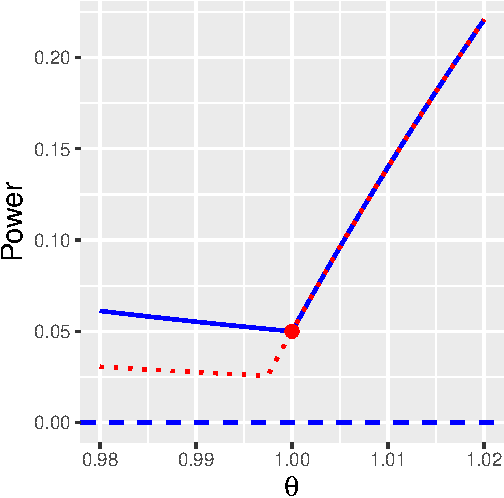
\includegraphics[keepaspectratio]{05-uniform_files/figure-latex/fig-uhyppow12-1.pdf}}

}

\caption{\label{fig-uhyppow12}The power curves for tests of
\(H_o : \theta = \theta_o = 1\) versus \(H_a : \theta \neq \theta_o\)
(red dotted line) and versus \(H_a : \theta \leq \theta_o\) (blue solid
line), assuming \(n = 10\). We observe that the one-tail test is more
powerful than the two-tail test if \(\theta < \theta_o\), and that the
tests are equally powerful if \(\theta \geq \theta_o\).}

\end{figure}%

\subsection{Example}\label{example-7}

\subsubsection{Pareto Domain Parameter: Hypothesis
Test}\label{pareto-domain-parameter-hypothesis-test}

\begin{quote}
We sample \(n\) iid data according to a Pareto(\(a,b\)) distribution,
with \(a\) fixed. We use these data to test \[
H_o: b = b_o ~~\mbox{versus}~~ H_a: b > b_o \,.
\] The sufficient statistic is the minimum datum \(X_{(1)}\); we can
appeal to reason to state that the expected value of this quantity must
increase as \(b\) increases, so we know that we are using the ``yes''
line of the hypothesis test reference tables and thus that
\(q = 1 - \alpha\). Borrowing from a previous example, we know that
\(F_{(1)}(x) = 1 - (b/x)^{na}\), hence \begin{align*}
F_Y(y \vert \theta) - q = 0 ~~~ &\Rightarrow ~~~ F_{(1)}(x_{\mathrm{RR}} \vert b_o) - (1-\alpha) = 0 \\
&\Rightarrow ~~~ 1 - \left(\frac{b_o}{x_{\mathrm{RR}}}\right)^{na} - (1 - \alpha) = \alpha - \left(\frac{b_o}{x_{\mathrm{RR}}}\right)^{na} = 0 \,.
\end{align*} Solving for \(x_{\mathrm{RR}}\), we find that \[
x_{\mathrm{RR}} = b_o \alpha^{-1/na} \,.
\]
\end{quote}

\begin{quote}
The \(p\)-value is straightforward to compute: according to the
reference tables, it is \begin{align*}
1 - F_Y(y_{\mathrm{obs}} \vert \theta_o) ~~~ \Rightarrow ~~~ 1 - F_{(1)}(x_{(1),\mathrm{obs}} \vert b_o) ~~~ \Rightarrow ~~~ \left(\frac{b_o}{x_{(1),\mathrm{obs}}}\right)^{na} \,.
\end{align*}
\end{quote}

\begin{quote}
However, as detailed mentioned above, the test power is less
straightforward to compute.
\end{quote}

\begin{quote}
If \(b > b_o\), then we can utilize the reference tables directly to
write that the power is \begin{align*}
1 - F_Y(y_{\mathrm{RR}} \vert \theta) ~~~ \Rightarrow ~~~ 1 - F_{(1)}(x_{\mathrm{RR}} \vert b) ~~~ \Rightarrow ~~~ \left(\frac{b}{x_{\mathrm{RR}}}\right)^{na} \,.
\end{align*} The power rises from \(\alpha\) to 1 as \(b\) decreases
from \(b_o\) to \(x_{\mathrm{RR}}\), and for larger values of \(b\) it
is 1 by definition (as it becomes impossible to sample a datum outside
of the rejection region). (See the left-hand side of
Figure~\ref{fig-uhyppow} and the left panel of
Figure~\ref{fig-uhyppow2}.)
\end{quote}

\begin{quote}
If \(b < b_o\), then we would reject the null hypothesis if
\(x_{(1),\mathrm{obs}} > x_{\mathrm{RR}}\) \emph{or}
\(x_{(1),\mathrm{obs}} < b_o\). Thus \begin{align*}
P(\mbox{reject}~\mbox{null} \vert b) &= P(X_{(1)} > x_{\mathrm{RR}} \cup X_{(1)} < b_o \vert b) \\
&= \left[ 1 - F_{(1)}(x_{\mathrm{RR}} \vert b)\right] + F_{(1)}(b_o \vert b)] \\
&= \left(\frac{b}{x_{\mathrm{RR}}}\right)^{na} + \left( 1 - \left(\frac{b}{b_o}\right)^{na} \right) \,.
\end{align*} (See the right-hand side of Figure~\ref{fig-uhyppow} and
the right panel of Figure~\ref{fig-uhyppow2}.)
\end{quote}

\begin{figure}

\centering{

\pandocbounded{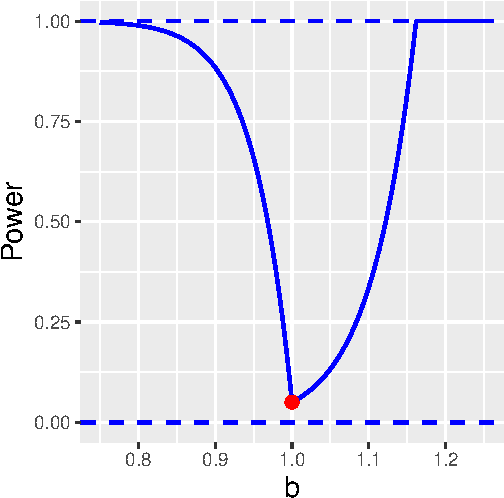
\includegraphics[keepaspectratio]{05-uniform_files/figure-latex/fig-uhyppow-1.pdf}}

}

\caption{\label{fig-uhyppow}The power curve for the test of
\(H_o : b = b_o = 1\) versus \(H_a : b > b_o\), assuming \(a = 2\) and
\(n = 10\). The curve displays two segments, and it achieves its minimum
value, \(\alpha = 0.05\), at \(b = 1\).}

\end{figure}%

\begin{figure}

\begin{minipage}[t]{0.50\linewidth}

\centering{

\pandocbounded{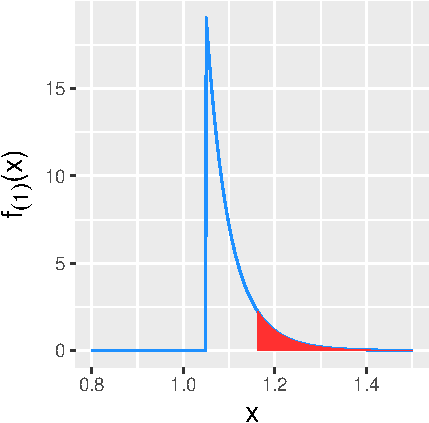
\includegraphics[keepaspectratio]{05-uniform_files/figure-latex/fig-uhyppow2-1.pdf}}

}

\subcaption{\label{fig-uhyppow2-1}}

\end{minipage}%
%
\begin{minipage}[t]{0.50\linewidth}

\centering{

\pandocbounded{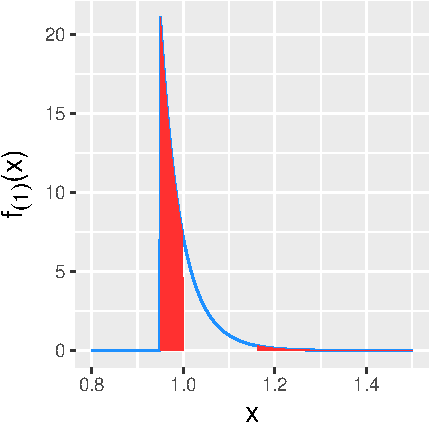
\includegraphics[keepaspectratio]{05-uniform_files/figure-latex/fig-uhyppow2-2.pdf}}

}

\subcaption{\label{fig-uhyppow2-2}}

\end{minipage}%

\caption{\label{fig-uhyppow2}The rejection regions that inform the power
curve calculation shown in Figure~\ref{fig-uhyppow}. (a) If \(b > b_o\),
then we reject the null hypothesis if
\(x_{(1),\mathrm{obs}} > x_{\mathrm{RR}}\). The power is thus the area
under the curve shown in red. (b) If \(b < b_o\), then we reject the
null hypothesis if \(x_{(1),\mathrm{obs}} > x_{\mathrm{RR}}\) or if
\(x_{(1),\mathrm{obs}} < b_o = 1\). The power is thus the sum of the two
areas under the curve shown in red.}

\end{figure}%

\begin{center}\rule{0.5\linewidth}{0.5pt}\end{center}

\section{Exercises}\label{sec-chap5exercises}

\begin{enumerate}
\def\labelenumi{\arabic{enumi}.}
\item
  Let \(X_1, X_2, \ldots, X_n\) denote independent and identically
  distributed uniform random variables on the interval \([0, 3\theta]\).
  Derive the method-of-moments estimator for \(\theta\).
\item
  Compute \(P(X > a+b \vert X > b)\) for a Uniform(0,1) distribution.
  (Assume \(0 < b < a+b < 1\).) Does the Uniform(0,1) distribution
  exhibit the property of memorylessness? Why or why not?
\item
  A woman goes to her local bus stop every day at a random time between
  noon and 1 PM, for five days total. If a bus doesn't appear to pick
  her up within 10 minutes, she immediately hops into a waiting Uber and
  is driven off. On every day, there is only one bus that will arrive
  between noon and 1:10 PM, and it will arrive at a random time \(X\)
  minutes after noon. \(X\) is sampled from the following distribution:
  \begin{eqnarray*}
  f_X(x) = \left\{ \begin{array}{ll} 1/70 & x \in [0,70] \\ 0 & \mbox{otherwise} \end{array} \right. \,.
  \end{eqnarray*} (a) On any one day, what is the probability that the
  woman catches the bus? (b) Over the five days, what is the probability
  that the woman catches the bus one or more times? (You may leave
  fractions raised to powers in your final answer, such as \((3/4)^3\)
  or \((7/15)^5\), if they are part of your answer.) (Also, if you are
  in doubt about your answer to (a), just use the variable \(p\) in
  place of your answer for (a) in part (b).)
\item
  You sample a datum \(X\) from a Uniform(0,1) distribution. What is
  \(P(X \leq 2u \vert X \geq u])\), where \(0 \leq u \leq 0.5\)?
\item
  Let \(X_1\) and \(X_2\) be two iid random variables sampled from a
  Uniform(0,1) distribution. What is \(P(X_1 < 2X_2 \vert X_2 < 1/2)\)?
  (Note: \(X_1\) and \(X_2\) are \emph{not} order statistics, so do not
  treat them as such!)
\item
  Assume that we have sampled \(n\) iid random variables from a
  Uniform(\(\theta,0\)) distribution, where \(\theta < 0\). (a) What is
  a sufficient statistic for \(\theta\)? (b) What is the cdf for this
  sufficient statistic? Be careful when deriving \(F_X(x)\): the pdf
  \(f_X(x)\) is \(1/(0-\theta) = -1/\theta\) and not \(1/\theta\). Also,
  take care when writing down the integral bounds. (c) We wish to test
  \(H_o : \theta = \theta_o\) versus \(H_a : \theta \neq \theta_o\).
  Recall that hypothesis tests are written down (in theory!) before the
  collection of data. Given that factoid, write down the trivial part of
  the test rejection region, i.e., the part of the overall rejection
  region that one can write down without having to work with the
  sufficient statistic cdf. (d) To derive the other part of the
  rejection region, do we set the cdf for the sufficient statistic to
  \(1-\alpha\) or \(1-\alpha/2\)? Choose one and write it in the answer
  box. Recall that the power of the hypothesis test when
  \(\theta = \theta_o\) is exactly \(\alpha\). (e) Given your answers
  for (b) and (d), derive the boundary of the other part of the
  rejection region (the non-trivial part).
\item
  You sample \(n\) iid data from the following (unnamed) distribution:
  \begin{eqnarray*}
  f_X(x) = \frac{2}{\theta^2} x  ~~~ x \in [0,\theta] \,.
  \end{eqnarray*} The cdf for this distribution is
  \(F_X(x) = (x/\theta)^2\). (a) What is the MLE for \(\theta\)? (b)
  What is \(E[X_{(n)}]\)? (c) What is the MVUE for \(\theta\)?
\item
  Let's assume we have sampled \(n\) iid data from the following
  distribution: \begin{align*}
  f_X(x) = e^{-(x-\theta)} ~~~ x \in [\theta,\infty)
  \end{align*} where \(\theta > 0\). The cdf for this distribution, for
  \(x \geq \theta\), is \begin{align*}
  F_X(x) = 1-e^{-(x-\theta)} \,.
  \end{align*} (a) Identify a sufficient statistic for \(\theta\). (b)
  Identify the maximum likelihood estimator for \(\theta\). No work need
  be shown. (c) Determine the sampling distribution (specifically, the
  pdf, and not the cdf) for the sufficient statistic identified in part
  (a). (d) Determine the minimum variance unbiased estimator for
  \(\theta\). You will want to utilize a variable subsitution here.
  Recall that \begin{align*}
  \Gamma(a+1) = a! = \int_0^\infty u^a e^{-u} du \,,
  \end{align*} assuming that \(a\) is a non-negative integer. (Also
  recall that 0! = 1.)
\item
  We sample two iid data, \(X_1\) and \(X_2\), from a Uniform(0,1)
  distribution. (a) What is \(P(X_1 > 1/2 \vert X_2 < 1/2)\)? (b) What
  is \(P(X_1 > 1/2 \vert X_1 < 3/4)\)? (c) What is \(P(X_1 < 3X_2)\)?
  (Hint: draw this out in a 1 \(\times\) 1 box. Do the same for (d).)
  (d) What is \(P(X_2 < X_1 \vert X_2 < 1/2)\)?
\item
  Let's assume that we have sampled \(n\) iid data from a particular
  distribution with domain \([\theta,\infty)\), and let the cdf of the
  sampling distribution of the appropriate statistic \(Y\) to use to
  construct confidence intervals and perform hypothesis tests be
  \begin{align*}
  F_Y(y) = 1 - e^{-n(y-\theta)} \,.
  \end{align*} Assume the observed statistic value is
  \(y_{\mathrm{obs}}\), and that \(E[Y] = \theta + 1/n\). (Note that it
  is not necessary to know what \(Y\) actually represents to answer the
  questions below.) (a) Determine a \(100(1-\alpha)\)-percent lower
  bound on \(\theta\). (b) Assume we wish to test
  \(H_o : \theta = \theta_o\) versus \(H_a : \theta \neq \theta_o\).
  Derive the rejection-region boundary (or boundaries)
  \(y_{\mathrm{RR}}\) in terms of \(\theta_o\), the Type I error
  \(\alpha\), and \(n\).
\item
  We are given the following probability mass function (which is an
  example of a discrete uniform distribution): \begin{align*}
  p_X(x) = 1/2 
  \end{align*} for \(x \in \{1,2\}\). (a) Compute the moment-generating
  function for this distribution. (b) Using the mgf, compute the
  variance of \(X\). Do not compute \(V[X]\) by any other method!
\item
  We sample a random variable \(X\) from a Uniform(0,1) distribution.
  Let \(U = \sqrt{X}\). (a) Write down the pdf for \(U\). (b) Identify
  the distribution of \(U\), if it is known. Include the name and any
  parameter values.
\item
  Let \(X \sim\) Uniform(0,1), i.e., \begin{eqnarray*}
  f_X(x) = 1
  \end{eqnarray*} for \(x \in [0,1]\). Now, let \(U = X^2\). (a) We will
  derive \(f_U(u)\) in part (c). For now: what is the domain of this
  probability density function? (b) What is the functional form of
  \(F_U(u)\) within the domain of \(f_U(u)\)? (c) What is the functional
  form of \(f_U(u)\) within its domain? (d) What is \(E[U]\)?
\item
  In an experiment, we sample \emph{one datum} according to the
  cumulative distribution function \begin{eqnarray*}
  F_X(x) = c\left( 1 - e^{-x/\theta} \right) \,,
  \end{eqnarray*} where \(x \in [0,-\theta\log(1-1/c)]\) (and where
  \(\theta\) is a known positive constant). One may picture this as a
  distribution that is truncated at the coordinate
  \(x_c = -\theta\log(1-1/c)\), with the unknown parameter \(c > 0\)
  having a value such that the integral of \(f_X(x)\) over the whole
  domain is 1. (a) What is the functional form of \(f_X(x)\)? (b) We
  wish to test the hypothesis \(H_o : c = c_o\) versus
  \(H_a : c > c_o\). What is the rejection region boundary
  \(x_{\mathrm{RR}}\) for this test? The answer should be in terms of
  \(\theta\), \(c_o\), and the level of the test \(\alpha\). (c) What is
  the power of the test given an arbitrary value \(c\), where
  \(c_o < c < c'\) and where \(c'\) is the value of \(c\) where the
  power achieves the value 1? Leave the answer in terms of \(c\) and
  \(x_{\mathrm{RR}}\). (d) Over what range of observed values of \(X\)
  would we trivially reject the null hypothesis, since if the null is
  correct, it would be impossible to observe values in this range? (e)
  If instead of sampling one datum, we sample \(n\) iid data, what would
  be a sufficient statistic for \(c\)?
\item
  In an experiment, we sample \emph{one datum} \(X\) according to the
  distribution \begin{eqnarray*}
  f_X(x) = \frac{2}{\theta}\left(1-\frac{x}{\theta}\right) ~~~~~~ x \in [0,\theta] \,.
  \end{eqnarray*} (a) What is the maximum likelihood estimate for
  \(\theta\)? (b) What is the expected value \(E[X]\)? (c) What is the
  bias of the MLE? (d) What is the minimum variance unbiased estimator
  for \(\theta\)? (e) One can compute that \(V[X] = \theta^2/18\). It
  turns out that the mean-squared errors for the MLE and the MVUE are
  the same, as a function of \(\theta\). Write down an expression for
  the MSE.
\end{enumerate}

\bookmarksetup{startatroot}

\chapter{Multivariate Distributions}\label{sec-chap6}

In this chapter, we move away from independent and identically
distributed data to examining the situation in which
\(\{X_1,\ldots,X_p\}\) are \(p\) random variables that are
\emph{jointly} sampled according to some \emph{multivariate
distribution} \(P\). Our focus will not be on statistical inference, but
on how one works with (specifically) bivariate probability
distributions: assessing the independence of random variables, computing
the covariance and correlation between them, deriving marginal and
conditional distributions, and working with conditional expected value
and variance. (While noting that any results that we write down for
bivariate distributions can be generalized to higher-dimensional ones as
well.)

Thus far we have looked at \emph{univariate probability distributions},
i.e., we have assumed that there is a single random variable \(X\) that
maps the events in a sample space to the real-number line. The quantity
represented by \(X\) might be, for instance, height or weight.

In this chapter, we shift to the \emph{multivariate} case, wherein we
might have \(p\) random variables \(\mathbf{X} = \{X_1,\ldots,X_p\}\)
representing, e.g., height \emph{and} weight (if \(p = 2\)). When there
are a set of \(p\) random variables, they are sampled from a joint
\(p\)-dimensional probability mass or density function that encapsulates
how the random variables are jointly distributed. (It can be the case
that the set can contain both discrete \emph{and} continuous random
variables, but for simplicity we will ignore that possibility here.)
Both joint pmfs \(p_{X_1,\ldots,X_p}(x_1,\ldots,x_p)\) and joint pdfs
\(f_{X_1,\ldots,X_p}(x_1,\ldots,x_p)\) have similar properties as their
univariate counterparts: they are non-negative (with
\(p_{X_1,\ldots,X_p}(x_1,\ldots,x_p) \leq 1\)) and they either sum or
integrate to 1. They is nothing ``special'' about these functions; they
are simply more mathematically complex and thus often less easy to work
with. However, there are new concepts for us to cover that only arise in
a multivariate context.

\begin{itemize}
\tightlist
\item
  \emph{Independence of Random Variables}: do the sampled values for one
  random variable (e.g., heights) depend on the sampled values for the
  others (e.g., weights)? If not, the random variables are independent.
  (In this simple example, we expect that heights and weights to be very
  much dependent: on average, taller people are heavier.)
\item
  \emph{Covariance and Correlation}: these metrics build upon the
  concept of variance and indicate the amount of \emph{linear}
  dependence between two random variables.
\item
  \emph{Marginal Distributions}: these show how a subset of the random
  variables is (jointly) distributed, without regard to the values taken
  on by the other random variables. For instance, if
  \(f_{X_h,X_W}(x_h,x_w)\) represents the joint distribution of heights
  and weights in a population, then the marginal distribution
  \(f_{X_h}(x_h)\) represents how heights are distributed, without
  regard to weight.
\item
  \emph{Conditional Distributions}: these show how a subset of the
  random variables is (jointly) distributed, conditional on the other
  random variables taking on specific values. For instance, the
  conditional distribution \(f_{X_h \vert X_w}(x_h \vert x_w)\)
  indicates the distribution of heights given a specific weight.
\item
  \emph{Conditional Expectation and Variance}: these metrics represent
  the mean and ``width'' of conditional distributions.
\end{itemize}

Note that throughout this chapter, we will illustrate concepts using
bivariate distributions, as adding mathematical complexity by increasing
dimensionality provides no additional benefit in terms of conceptual
understanding. The one exception to this is in the last section, where
we discuss the multivariate normal distribution.

\section{Independence of Random Variables}\label{sec-chap6independence}

What to take away from this section:

\begin{itemize}
\item
  Two random variables \(X_1\) and \(X_2\) that are sampled according to
  a bivariate probability density function \(f_{X_1,X_2}(x_1,x_2)\) are
  \emph{independent} random variables if\ldots{}

  \begin{itemize}
  \item
    no part of the boundary of the domain of \(f_{X_1,X_2}(x_1,x_2)\)
    depends on both the coordinates \(x_1\) \emph{and} \(x_2\); and
  \item
    if \(f_{X_1,X_2}(x_1,x_2)\) can be factored into two functions, one
    that is only a function of \(x_1\) and one that is only a function
    of \(x_2\).
  \end{itemize}
\end{itemize}

At the end of Section~\ref{sec-chap1statistics}, we describe at a high
level the concept of two or more random variables being independent of
each other. In that chapter, we give the example of a \emph{bivariate
probability density function}, i.e., a function which outputs the
probability density given \emph{two} inputs, \(x_1\) and \(x_2\):
\(f_{X_1,X_2}(x_1,x_2)\). To test for independence, we need only inspect
the functional form of \(f_{X_1,X_2}(x_1,x_2)\) and its domain; \(X_1\)
and \(X_2\) are independent if and only if

\begin{itemize}
\tightlist
\item
  the boundaries of the domain depend on either \(x_1\) or \(x_2\) but
  not both at the same time (i.e., the domain is ``rectangular''); and
\item
  \(f_{X_1,X_2}(x_1,x_2)\) can be factored into the product of functions
  that only depend on \(x_1\) and on \(x_2\), respectively:
  \(f_{X_1}(x_1) \times
  f_{X_2}(x_2)\).
\end{itemize}

(Furthermore, we state that if \(f_{X_1}(x_1) = f_{X_2}(x_2)\), then
\(X_1\) and \(X_2\) are iid random variables.)

If either condition given above does not hold, then we conclude that
\(X_1\) and \(X_2\) are dependent random variables.

\subsection{Example}\label{example-8}

\subsubsection{Determining Whether Two Random Variables are
Independent}\label{determining-whether-two-random-variables-are-independent}

\begin{quote}
Let \(X_1\) and \(X_2\) have the following joint pdf: \[
f_{X_1,X_2}(x_1,x_2) = c(1-x_2) 
\] for \(0 \leq x_1 \leq x_2 \leq 1\). For now, we are not concerned
with the value of the constant \(c\). Are \(X_1\) and \(X_2\)
independent random variables?
\end{quote}

\begin{quote}
The first thing to do is inspect the joint domain. This can be tricky,
and it is often best to break the statement of the domain up into
multiple ``pieces.'' Here, we can say that first, we know that
\(x_1 \in [0,1]\) and that \(x_2 \in [0,1]\). This limits the domain to
a box on the \(x_1\)-\(x_2\) plane. (See the axes and the red dashed
lines in Figure~\ref{fig-mulfig1}.) Furthermore, we know that
\(x_1 \leq x_2\), or, equivalently, that \(x_2 \geq x_1 + 0\), i.e.,
that \(x_2\) lies above a line with slope one and intercept zero. (See
the orange short-dashed line in Figure~\ref{fig-mulfig1}.) Given that
the domain is triangular, we can state unequivocally here that \(X_1\)
and \(X_2\) are \emph{not} independent random variables. In particular,
we do not need to check whether
\(f_{X_1,X_2}(x_1,x_2) = f_{X_1}(x_1) \times f_{X_2}(x_2)\).
\end{quote}

\begin{figure}

\centering{

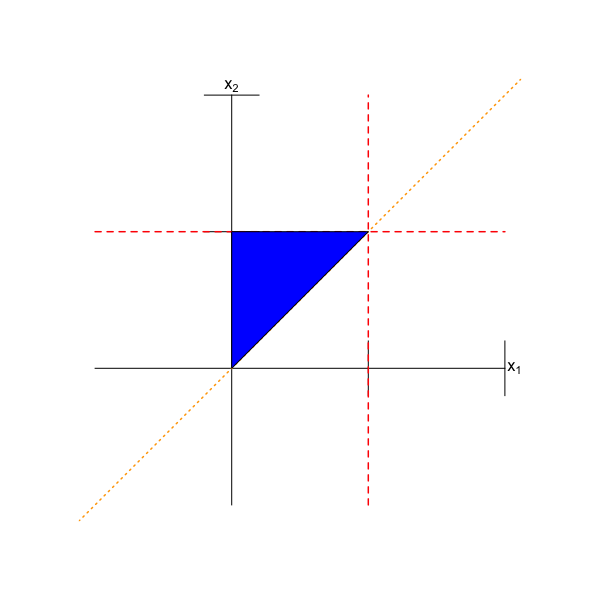
\includegraphics[width=0.75\linewidth,height=\textheight,keepaspectratio]{figures/multi_fig1.png}

}

\caption{\label{fig-mulfig1}The domain of \(f_{X_1,X_2}(x_1,x_2)\),
expressed mathematically as \(0 \leq x_1 \leq x_2 \leq 1\). The red
dashed lines indicate that \(0 \leq x_1 \leq 1\) and
\(0 \leq x_2 \leq 1\), and the orange short-dashed line indicates that
\(x_2 \geq x_1\). The blue triangle is the domain of the function.}

\end{figure}%

\begin{quote}
As a second example, let \(X_1\) and \(X_2\) have the following joint
pdf: \[
f_{X_1,X_2}(x_1,x_2) = ce^{-x_1x_2} \,,
\] where \(0 \leq x_1 \leq 1\) and \(0 \leq x_2 \leq 1\). Again, we are
not concerned about the value of \(c\), at least for now. Are \(X_1\)
and \(X_2\) independent random variables?
\end{quote}

\begin{quote}
We can see by inspection that the domain is ``rectangular,''
specifically a square with vertices (0,0), (0,1), (1,0), and (1,1). So
far, so good. Can we factor \(f_{X_1,X_2}(x_1,x_2)\) into two separate
functions that depend only on \(x_1\) or only on \(x_2\)? The answer is
no. (As a reminder, \(e^{ab} \neq e^a e^b\)!) Hence we can state that
\(X_1\) and \(X_2\) are \emph{not} independent random variables.
\end{quote}

\section{Properties of Multivariate
Distributions}\label{sec-chap6properties}

What to take away from this section:

\begin{itemize}
\tightlist
\item
  The probability mass and density functions of bivariate (and more
  generally, multivariate) distributions have the same properties as
  their univariate counterparts: they are non-negative, sum or integrate
  to one over their domains, can be characterized via expected value and
  variance, and have cumulative distribution functions. They simply are
  defined along more than one coordinate axis.
\end{itemize}

As stated in Section~\ref{sec-chap1random}, a probability distribution
is a mapping \(P : \Omega \rightarrow \mathbb{R}^n\), where \(\Omega\)
is the sample space for an experiment. This mapping describes how
probabilities are distributed across the values of a random variable. In
the first five chapters, \(n = 1\), meaning that we focus on univariate
distributions. Here, however, \(n > 1\), with the bulk of our discussion
focusing upon the case \(n = 2\). Nothing changes, fundamentally, when
we work with multivariate distributions: (a) they are non-negative; and
(b) they sum or integrate to 1. Assuming \(n = 2\), we can write that

{\def\LTcaptype{none} % do not increment counter
\begin{longtable}[]{@{}
  >{\centering\arraybackslash}p{(\linewidth - 2\tabcolsep) * \real{0.5000}}
  >{\centering\arraybackslash}p{(\linewidth - 2\tabcolsep) * \real{0.5000}}@{}}
\toprule\noalign{}
\begin{minipage}[b]{\linewidth}\centering
joint pmf
\end{minipage} & \begin{minipage}[b]{\linewidth}\centering
joint pdf
\end{minipage} \\
\midrule\noalign{}
\endhead
\bottomrule\noalign{}
\endlastfoot
\(p_{X_1,X_2}(x_1,x_2) \in [0,1]\) &
\(f_{X_1,X_2}(x_1,x_2) \in [0,\infty)\) \\
\(\sum_{x_1} \sum_{x_2} p_{X_1,X_2}(x_1,x_2) = 1\) &
\(\int_{x_1} \int_{x_2} f_{X_1,X_2}(x_1,x_2) dx_2 dx_1 = 1\) \\
\end{longtable}
}

We will reiterate that the joint pdf \(f_{X_1,X_2}(x_1,x_2)\) is not the
probability of sampling the tuple \((x_1,x_2)\) but rather is a
probability density; to determine probabilities, we would invoke
multi-dimensional integration: \[
P(a_1 \leq X_1 \leq b_1,a_2 \leq X_2 \leq b_2) = \int_{a_1}^{b_1} \int_{a_2}^{b_2} f_{X_1,X_2}(x_1,x_2) dx_2 dx_1 \,.
\]

As for the joint cumulative distribution function, or joint cdf, the
convention is to treat each axis separately from the others, i.e., to
define it as \[
F_{X_1,X_2}(x_1,x_2) = P(X_1 \leq x_1 \cap X_2 \leq x_2) \,.
\] The joint cdf satisfies the following properties:

\begin{itemize}
\tightlist
\item
  if either \(X_i = -\infty\), the joint cdf is zero;
\item
  if both \(X_i = \infty\), the joint cdf is one;
\item
  it increases monotonically along each coordinate axis; and
\item
  if \(X_1\) and \(X_2\) are independent random variables, then
  \(F_{X_1,X_2}(x_1,x_2) = F_{X_1}(x_1) F_{X_2}(x_2)\).
\end{itemize}

To characterize bivariate distributions (and multivariate ones in
general), we compute distribution moments by utilizing the Law of the
Unconscious Statistician: \begin{align*}
E[g(X_1,X_2)] &= \sum_{x_1} \sum_{x_2} g(x_1,x_2) p_{X_1,X_2}(x_1,x_2) \qquad \mbox{discrete}\\
&= \int_{x_1} \int_{x_2} g(x_1,x_2) f_{X_1,X_2}(x_1,x_2) dx_2 dx_1 \qquad \mbox{continuous} \,,
\end{align*} with the shortcut formula continuing to hold in the
multivariate case: \[
V[g(X_1,X_2)] = E\left[ g(X_1,X_2)^2 \right] - (E[g(X_1,X_2)])^2 \,.
\]

We note that if we write \(g(x_1,x_2)\) as \(g_1(x_1)g_2(x_2)\) and if
\(X_1\) and \(X_2\) are independent random variables, then
\begin{align*}
E[g_1(X_1)g_2(X_2)] &= \int_{x_1} \int_{x_2} g_1(x_1) g_2(x_2) f_{X_1,X_2}(x_1,x_2) dx_2 dx_1 \\
&= \int_{x_1} \int_{x_2} g_1(x_1) g_2(x_2) f_{X_1}(x_1) f_{X_2}(x_2) dx_2 dx_1 \\
&= \left[ \int_{x_1} g_1(x_1) f_{X_1}(x_1) \right] \cdot \left[ \int_{x_2} g_2(x_2) f_{X_2}(x_2) \right] \\
&= E[g_1(X_1)] E[g_2(X_2)] \,.
\end{align*} So, for instance, \(E[X_1X_2] = E[X_1]E[X_2]\) if \(X_1\)
and \(X_2\) are independent, but not generally.

\subsection{Examples}\label{examples-47}

\subsubsection{Characterizing a Discrete Bivariate
Distribution}\label{characterizing-a-discrete-bivariate-distribution}

\begin{quote}
Let \(X_1\) and \(X_2\) have the following joint probability mass
function \(p_{X_1,X_2}(x_1,x_2)\):
\end{quote}

{\def\LTcaptype{none} % do not increment counter
\begin{longtable}[]{@{}cccc@{}}
\toprule\noalign{}
\endhead
\bottomrule\noalign{}
\endlastfoot
& \(x_2 = 0\) & \(x_2 = 1\) & \(x_2 = 2\) \\
\(x_1 = 1\) & 0.20 & 0.30 & 0.00 \\
\(x_1 = 2\) & 0.40 & 0.00 & 0.10 \\
\end{longtable}
}

\begin{quote}
What is \(E[X_1X_2]\)?
\end{quote}

\begin{quote}
We utilize the Law of the Unconscious Statistician: \begin{align*}
E[X_1X_2] &= \sum_{x_1} \sum_{x_2} x_1 x_2 p_{X_1,X_2}(x_1,x_2) \\
&= 1 \times 0 \times 0.20 + 2 \times 0 \times 0.40 + 1 \times 1 \times 0.30 + 2 \times 2 \times 0.10 \\
&= 0.30 + 0.40 = 0.70 \,.
\end{align*}
\end{quote}

\begin{quote}
What is \(F_{X_1,X_2}(3/2,3/2)\)?
\end{quote}

\begin{quote}
The joint cdf is \begin{align*}
P(X_1 \leq 3/2 \cap X_2 \leq 3/2) &= P(X_1 = 1 \cap X_2 = 0) + P(X_1 = 1 \cap X_2 = 1) \\
&= 0.20 + 0.30 = 0.50 \,.
\end{align*}
\end{quote}

\subsubsection{Characterizing a Continuous Bivariate
Distribution}\label{characterizing-a-continuous-bivariate-distribution}

\begin{quote}
Let \(X_1\) and \(X_2\) have the following joint probability density
function: \[
f_{X_1,X_2}(x_1,x_2) = c(1-x_2) \,,
\] with \(0 \leq x_1 \leq x_2 \leq 1\). In an example above, we
determined that \(X_1\) and \(X_2\) are dependent random variables due
to the domain of the pdf not being ``rectangular'' on the
\(x_1\)-\(x_2\) plane (see Figures Figure~\ref{fig-mulfig1} and
Figure~\ref{fig-bivar1}).
\end{quote}

\begin{quote}
Here, we will first determine the value of \(c\) that makes this
function a valid joint pdf. Carrying out this calculation will involve
double integration. We note here that we can integrate in either order
(i.e., along the \(x_1\) axis first, or the \(x_2\) axis first), as the
final result will be the same. Here, we will integrate along \(x_1\)
first, since the lower bound along this axis is zero (a choice which
often simplifies the overall calculation) \emph{and} because \(x_1\)
does not appear in the integrand: \begin{align*}
\int_0^1 \left[ \int_0^{x_1 = x_2} c (1-x_2) dx_1 \right] dx_2 &= c \int_0^1 (1-x_2) \left[ \int_0^{x_1 = x_2} dx_1 \right] dx_2 \\
&= c \int_0^1 (1-x_2) \left[ \left. x_1 \right|_0^{x^2} \right] dx_2 \\
&= c \int_0^1 x_2 (1-x_2) dx_2 \\
&= c B(2,2) = c \Gamma(2) \Gamma(2) / \Gamma(4) \\
&= c \times 1! \times 1! / 3! = c/6 = 1 \,.
\end{align*} Thus \(c = 6\). Note that we take advantage of the fact
that \(x_2 (1-x_2)\) integrated from 0 to 1 is a Beta(2,2) distribution.
If we had not made that association, we would still have observed the
same final solution after integrating the polynomial in the integrand.
\end{quote}

\begin{figure}

\centering{

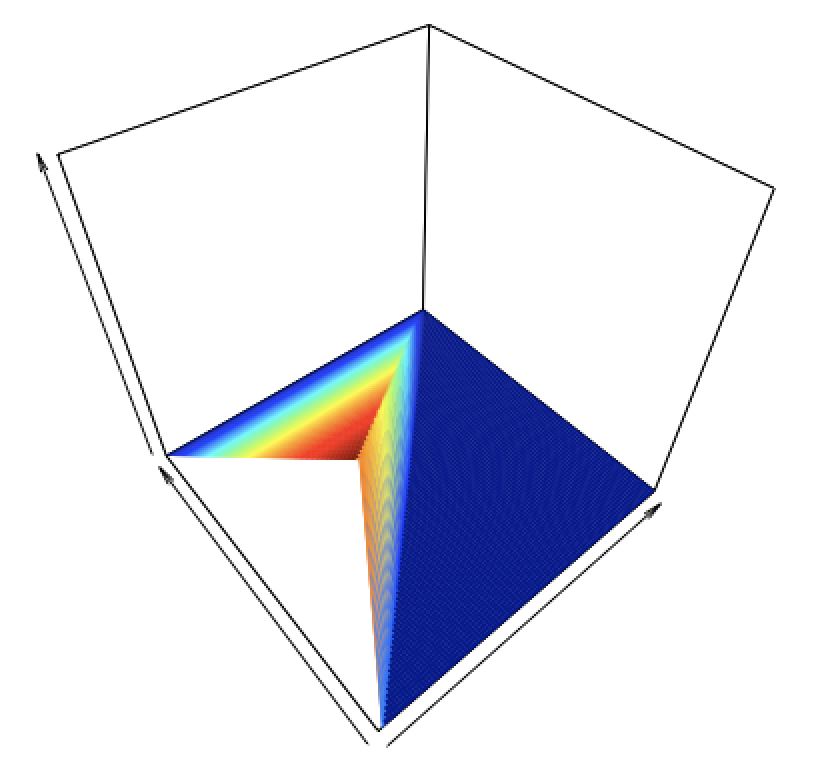
\includegraphics[width=0.75\linewidth,height=\textheight,keepaspectratio]{figures/bivar1.png}

}

\caption{\label{fig-bivar1}\label{fig-bivar1}The probability density
function \(6(1-x_2)\) as a function of \(x_1\) (axis pointing to upper
right) and \(x_2\) (axis pointing to upper left). The pdf peaks at
\((x_1,x_2) = (0,0)\) and falls off towards \(x_2 = 1\) as a plane, with
value greater than zero only within the domain
\(0 \leq x_1 \leq x_2 \leq 1\); Figure~\ref{fig-mulfig1} shows that
domain.}

\end{figure}%

\begin{quote}
Now we will ask, what are \(E[X_2]\) and \(V[X_2]\)? \begin{align*}
E[X_2] &= \int_0^1 \left[ \int_0^{x_1 = x_2} 6 x_2 (1-x_2) dx_1 \right] dx_2 \\
&= 6 \int_0^1 x_2 (1-x_2) \left[ \int_0^{x_1 = x_2} dx_1 \right] dx_2 \\
&= 6 \int_0^1 x_2 (1-x_2) \left[ \left. x_1 \right|_0^{x^2} \right] dx_2 \\
&= 6 \int_0^1 x_2^2 (1-x_2) dx_2 \\
&= 6 B(3,2) = 6 \Gamma(3) \Gamma(2) / \Gamma(5) = 6 \times 2! \times 1! / 4! = 1/2 \,.
\end{align*} In a similar manner, we can determine that \begin{align*}
E[X_2^2] &= 6 B(4,2) = 6 \times 3! \times 1! / 5! = 36/120 = 3/10 \\
V[X_2] &= E[X_2^2] - (E[X_2])^2 = 3/10 - 1/4 = 1/20 \,.
\end{align*}
\end{quote}

\subsubsection{Using Numerical Integration to Characterize a Continuous
Bivariate
Distribution}\label{using-numerical-integration-to-characterize-a-continuous-bivariate-distribution}

\begin{quote}
In the previous example, we assumed that the random variables \(X_1\)
and \(X_2\) were distributed according to the joint probability density
function \begin{align*}
f_{X_1,X_2}(x_1,x_2) = c(1-x_2) \,,
\end{align*} with \(0 \leq x_1 \leq x_2 \leq 1\), and we determined the
normalization value \(c\) and the expected value and variance of \(X_2\)
via double integration. Here, we demonstrate how the
\texttt{integral2()} function of the \texttt{pracma} package can help us
perform the same calculations numerically.
\end{quote}

\begin{Shaded}
\begin{Highlighting}[]
\FunctionTok{library}\NormalTok{(pracma)}

\CommentTok{\# Define the (finite) domain}
\NormalTok{x1min }\OtherTok{\textless{}{-}} \DecValTok{0}
\NormalTok{x1max }\OtherTok{\textless{}{-}} \DecValTok{1} 
\NormalTok{x2min }\OtherTok{\textless{}{-}} \ControlFlowTok{function}\NormalTok{(x1) \{ x1 \} }\CommentTok{\# the lower bound for x2 is the line x2=x1}
\NormalTok{x2max }\OtherTok{\textless{}{-}} \DecValTok{1}

\CommentTok{\# Determine c}
\NormalTok{f }\OtherTok{\textless{}{-}} \ControlFlowTok{function}\NormalTok{(x1,x2) \{}
  \DecValTok{1} \SpecialCharTok{{-}}\NormalTok{ x2}
\NormalTok{\}}
\NormalTok{I }\OtherTok{\textless{}{-}} \FunctionTok{integral2}\NormalTok{(f, x1min, x1max, x2min, x2max)}\SpecialCharTok{$}\NormalTok{Q}
\FunctionTok{cat}\NormalTok{(}\StringTok{"The value of c is"}\NormalTok{, }\DecValTok{1} \SpecialCharTok{/}\NormalTok{ I, }\StringTok{"}\SpecialCharTok{\textbackslash{}n}\StringTok{"}\NormalTok{)}
\end{Highlighting}
\end{Shaded}

\begin{verbatim}
The value of c is 6 
\end{verbatim}

\begin{Shaded}
\begin{Highlighting}[]
\CommentTok{\# Determine E[X2]}
\NormalTok{f }\OtherTok{\textless{}{-}} \ControlFlowTok{function}\NormalTok{(x1, x2) \{}
  \DecValTok{6} \SpecialCharTok{*}\NormalTok{ x2 }\SpecialCharTok{*}\NormalTok{ (}\DecValTok{1} \SpecialCharTok{{-}}\NormalTok{ x2)}
\NormalTok{\}}
\NormalTok{I }\OtherTok{\textless{}{-}} \FunctionTok{integral2}\NormalTok{(f, x1min, x1max, x2min, x2max)}\SpecialCharTok{$}\NormalTok{Q}
\FunctionTok{cat}\NormalTok{(}\StringTok{"E[X2] ="}\NormalTok{, I, }\StringTok{"}\SpecialCharTok{\textbackslash{}n}\StringTok{"}\NormalTok{)}
\end{Highlighting}
\end{Shaded}

\begin{verbatim}
E[X2] = 0.5 
\end{verbatim}

\begin{Shaded}
\begin{Highlighting}[]
\CommentTok{\# Determine E[X2\^{}2], and the variance}
\NormalTok{f }\OtherTok{\textless{}{-}} \ControlFlowTok{function}\NormalTok{(x1, x2) \{}
  \DecValTok{6} \SpecialCharTok{*}\NormalTok{ x2}\SpecialCharTok{\^{}}\DecValTok{2} \SpecialCharTok{*}\NormalTok{ (}\DecValTok{1} \SpecialCharTok{{-}}\NormalTok{ x2)}
\NormalTok{\}}
\NormalTok{J }\OtherTok{\textless{}{-}} \FunctionTok{integral2}\NormalTok{(f, x1min, x1max, x2min, x2max)}\SpecialCharTok{$}\NormalTok{Q}
\FunctionTok{cat}\NormalTok{(}\StringTok{"V[X2] ="}\NormalTok{, J }\SpecialCharTok{{-}}\NormalTok{ I}\SpecialCharTok{\^{}}\DecValTok{2}\NormalTok{, }\StringTok{"}\SpecialCharTok{\textbackslash{}n}\StringTok{"}\NormalTok{)}
\end{Highlighting}
\end{Shaded}

\begin{verbatim}
V[X2] = 0.05 
\end{verbatim}

\subsubsection{The Bivariate Uniform
Distribution}\label{the-bivariate-uniform-distribution}

\begin{quote}
The bivariate uniform distribution is defined as \[
f_{X_1,X_2}(x_1,x_2) = \frac{1}{A} \,,
\] where \(A\) is the area of the domain. (Thus the integral of the
bivariate function is \(A \times 1/A = 1\).) Let
\(f_{X_1,X_2}(x_1,x_2) = 1\) over the square defined by the vertices
(0,0), (0,1), (1,0), and (1,1). What is \(P(X_1 > 2X_2)\)?
\end{quote}

\begin{quote}
A nice feature of the bivariate uniform is that we can work with it
``geometrically'': if we can determine the fraction of the \emph{domain}
that abides by the stated condition, then we have our answer. (This is
because the joint pdf is flat, so integration is unnecessary.)
\end{quote}

\begin{quote}
We can rewrite \(x_1 > 2x_2\) as \(x_2 < x_1/2\), i.e., the region of
interest in the domain is the region below the line with intercept zero
and slope 1/2. (See Figure~\ref{fig-mulfig2}.) This region is a triangle
with vertices (0,0), (1,1/2), and (1,0), which has the area (recall:
one-half times base times height) \(1/2 \times 1 \times 1/2 = 1/4\).
Done! \(P(X_1 > 2X_2) = 1/4\).
\end{quote}

\begin{figure}

\centering{

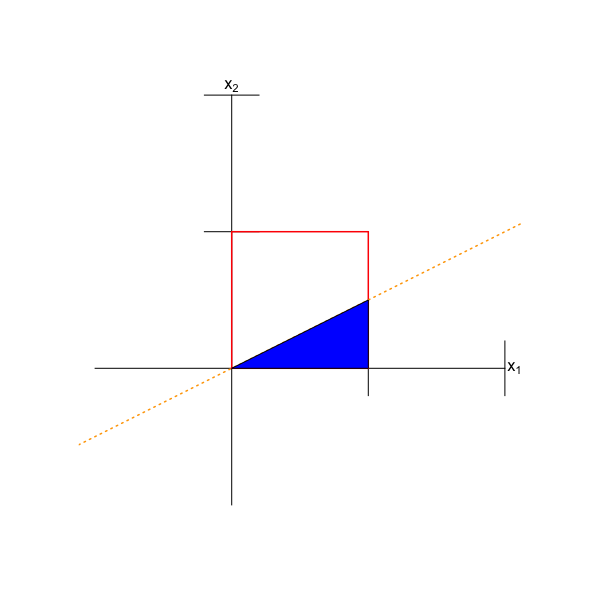
\includegraphics[width=0.75\linewidth,height=\textheight,keepaspectratio]{figures/multi_fig2.png}

}

\caption{\label{fig-mulfig2}The probability density function
\(6(1-x_2)\) as a function of \(x_1\) (axis pointing to upper right) and
\(x_2\) (axis pointing to upper left). The pdf peaks at
\((x_1,x_2) = (0,0)\) and falls off towards \(x_2 = 1\) as a plane, with
value greater than zero only within the domain
\(0 \leq x_1 \leq x_2 \leq 1\); Figure~\ref{fig-mulfig1} shows that
domain.}

\end{figure}%

\section{Covariance and Correlation}\label{sec-chap6covariance}

What to take away from this section:

\begin{itemize}
\item
  The \emph{covariance} between two random variables \(X_1\) and \(X_2\)
  is a metric that quantifies the amount of \emph{linear dependence}
  between them.
\item
  The \emph{correlation} between two random variables is the value of
  the covariance rescaled so as to lie between \(-1\) and 1; the
  rescaling aids interpretation.
\item
  Uncorrelated random variables (ones for which the value of the
  correlation is zero) are not necessarily independent random variables,
  but independent random variables are uncorrelated.
\end{itemize}

The \emph{covariance} between two random variables \(X_1\) and \(X_2\)
is a metric that quantifies the amount of \emph{linear dependence}
between them. (Other metrics of dependence, such as mutual information,
are beyond the scope of this book.) It is defined as \[
{\mathrm{Cov}}(X_1,X_2) = E[(X_1-\mu_1)(X_2-\mu_2)] \,,
\] but one rarely uses this expression, as there is a shortcut formula:
\begin{align*}
{\mathrm{Cov}}(X_1,X_2) &= E[X_1X_2 - X_1\mu_2 - X_2\mu_1 + \mu_1\mu_2] \\
&= E[X_1X_2] - \mu_2E[X_1] - \mu_1E[X_2] + \mu_1\mu_2 \\
&= E[X_1X_2] - E[X_2]E[X_1] - E[X_1]E[X_2] + E[X_1]E[X_2] \\
&= E[X_1X_2] - E[X_1]E[X_2] \,.
\end{align*} In the previous section, we saw that
\(E[X_1X_2] = E[X_1]E[X_2]\) if \(X_1\) and \(X_2\) are independent
random variables. Thus independent random variables have no covariance,
which makes sense: independent random variables would have by definition
no linear dependence. However, it is \emph{not} true that
\(E[X_1X_2] = E[X_1]E[X_2]\) \emph{implies} that \(X_1\) and \(X_2\) are
independent random variables\ldots it just implies there is no linear
dependence between the two variables. See Figure~\ref{fig-covplot1}.

\begin{figure}

\begin{minipage}[t]{0.33\linewidth}

\centering{

\pandocbounded{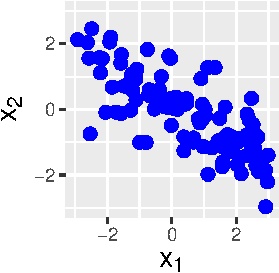
\includegraphics[keepaspectratio]{06-multivariate_files/figure-latex/fig-covplot1-1.pdf}}

}

\subcaption{\label{fig-covplot1-1}}

\end{minipage}%
%
\begin{minipage}[t]{0.33\linewidth}

\centering{

\pandocbounded{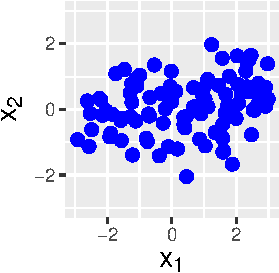
\includegraphics[keepaspectratio]{06-multivariate_files/figure-latex/fig-covplot1-2.pdf}}

}

\subcaption{\label{fig-covplot1-2}}

\end{minipage}%
%
\begin{minipage}[t]{0.33\linewidth}

\centering{

\pandocbounded{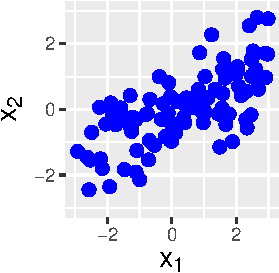
\includegraphics[keepaspectratio]{06-multivariate_files/figure-latex/fig-covplot1-3.pdf}}

}

\subcaption{\label{fig-covplot1-3}}

\end{minipage}%

\caption{\label{fig-covplot1}Examples of data with negative covariance
(a), no covariance (b), and positive covariance (c).}

\end{figure}%

Covariance is not necessarily an optimal metric for expressing linear
dependence, as its value is not readily interpretable. To see this,
assume we have the expression \((tX_1 - X_2)\) for some constant \(t\).
Then \((tX_1-X_2)^2 \geq 0\) and \(E[(tX_1-X_2)^2] \geq 0\). Thus
\begin{align*}
E[(tX_1-X_2)^2] &= E[t^2X_1^2 - 2tX_1X_2 + X_2^2] \\
&= E[X_1^2] t^2 - 2E[X_1X_2] t + E[X_2^2] \\
&= a t^2 + b t + c \geq 0 \,.
\end{align*} (Recall that expected values are constants, and not
themselves random variables.) The key here is that if
\(a t^2 + b t + c = 0\), there is one real root to this quadratic
equation, while if \(a t^2 + b t + c > 0\), there are no real roots.
Thus the discriminant, \(b^2 - 4ac\), must be \(\leq 0\), and so
\begin{align*}
b^2 - 4ac &= 4 (E[X_1X_2])^2 - 4 E[X_1^2] E[X_2^2] \leq 0 \\
\Rightarrow& (E[X_1X_2])^2 \leq E[X_1^2] E[X_2^2] \,.
\end{align*} At this point, the reader might ask ``well, what about
this?'' The expression to the left above, \((E[X_1X_2])^2\), is
\([{\mathrm{Cov}}(X_1,X_2)]^2\) when \(\mu_1 = \mu_2 = 0\), while the
expression to the right, \(E[X_1^2] E[X_2^2]\), is \(V[X_1]V[X_2]\) when
\(\mu_1 = \mu_2 = 0\). Thus \[
\vert {\mathrm{Cov}}(X_1,X_2) \vert \leq \sqrt{V[X_1]V[X_2]} = \sigma_1 \sigma_2 \,,
\] or
\(- \sigma_1 \sigma_2 \leq {\mathrm{Cov}}(X_1,X_2) \leq \sigma_1 \sigma_2\).
The fact that we may not know immediately the value of
\(\sigma_1 \sigma_2\) is what makes any numerical value of
\({\mathrm{Cov}}(X_1,X_2)\) hard to interpret.

Thus we conventionally turn to an alternate expression of linear
dependence, the \emph{correlation coefficient}: \[
\rho_{X_1,X_2} = \frac{{\mathrm{Cov}}(X_1,X_2)}{\sigma_1\sigma_2} \Rightarrow -1 \leq \rho \leq 1 \,.
\] If \(\rho_{X_1,X_2} < 0\), then an increase in the sampled value of
\(X_1\) is associated with, \emph{on average}, a smaller sampled value
of \(X_2\), i.e., \(X_1\) and \(X_2\) are negatively
correlated\ldots whereas if \(\rho_{X_1,X_2} > 0\), larger sampled
values for \(X_1\) are associated on average with larger sampled values
of \(X_2\), i.e., \(X_1\) and \(X_2\) are positively correlated.

(We note that we have actually seen \(\rho_{X_1,X_2}\) before, in
Section~\ref{sec-chap2slr}, when we introduced correlation as a metric
of the strength of linear association as measured in simple linear
regression. Recall that we estimate \(\rho_{X_1,X_2}\) with, e.g., the
Pearson correlation coefficient \(R\), and that we use coefficient of
determination \(R^2\) to quantify the usefulness of the linear
regression model. See Figure~\ref{fig-covplot2}.)

\begin{figure}

\begin{minipage}[t]{0.33\linewidth}

\centering{

\pandocbounded{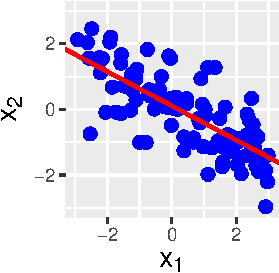
\includegraphics[keepaspectratio]{06-multivariate_files/figure-latex/fig-covplot2-1.pdf}}

}

\subcaption{\label{fig-covplot2-1}}

\end{minipage}%
%
\begin{minipage}[t]{0.33\linewidth}

\centering{

\pandocbounded{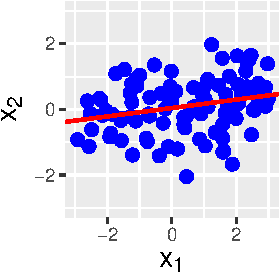
\includegraphics[keepaspectratio]{06-multivariate_files/figure-latex/fig-covplot2-2.pdf}}

}

\subcaption{\label{fig-covplot2-2}}

\end{minipage}%
%
\begin{minipage}[t]{0.33\linewidth}

\centering{

\pandocbounded{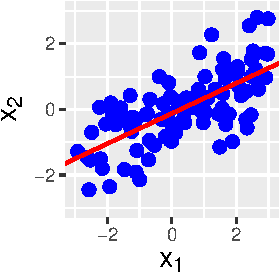
\includegraphics[keepaspectratio]{06-multivariate_files/figure-latex/fig-covplot2-3.pdf}}

}

\subcaption{\label{fig-covplot2-3}}

\end{minipage}%

\caption{\label{fig-covplot2}The same data as shown in
Figure~\ref{fig-covplot1}, with linear regression lines superimposed.
The estimated correlations are -0.752, 0.257, and 0.712, respectively,
from (a) to (c).}

\end{figure}%

\begin{center}\rule{0.5\linewidth}{0.5pt}\end{center}

Let's suppose we are given \(n\) correlated random variables
\(\{X_1,\ldots,X_n\}\), and we define the sum
\(Y = \sum_{i=1}^n a_i X_i\). Furthermore, let's assume we know the
pdf/pmf, expected value, and variance of each of the \(X_i\)'s. What do
we know about the distribution of \(Y\)? With work, we might be able to
determine its pdf or pmf, but we would have to go beyond the method of
moment-generating functions because that method requires the random
variables to be independent of each other. We will not do that here.
However, we \emph{can} determine the expected value of \(Y\): \[
E[Y] = E\left[ \sum_{i=1}^n a_i X_i \right] = \sum_{i=1}^n a_i E[X_i] \,.
\] Dependencies between the \(X_i\)'s does not affect this equality. As
for the variance of \(Y\)\ldots{}

We start by encapsulating the information about the covariances between
each variable pair into a \emph{covariance matrix}. For \(n\) random
variables, the \(n \times n\) covariance matrix \(\boldsymbol{\Sigma}\)
is \[
\boldsymbol{\Sigma} = \left[ \begin{array}{ccc} {\mathrm{Cov}}(X_1,X_1) & \cdots & {\mathrm{Cov}}(X_1,X_n) \\ \vdots & \ddots & \vdots \\ {\mathrm{Cov}}(X_n,X_1) & \cdots & {\mathrm{Cov}}(X_n,X_n) \end{array} \right] = \left[ \begin{array}{ccc} V[X_1] & \cdots & {\mathrm{Cov}}(X_1,X_n) \\ \vdots & \ddots & \vdots \\ {\mathrm{Cov}}(X_n,X_1) & \cdots & V[X_n] \end{array} \right] \,.
\] We note that the diagonal of this matrix (the elements from the upper
left corner to the lower right corner) contains the individual
variances, since Cov(\(X_i,X_i\)) = \(V[X_i]\), and that because
Cov(\(X_i,X_j\)) = Cov(\(X_j,X_i\)), the matrix is symmetric about the
diagonal.

Now, let \(a^T = [ a_1 ~ a_2 ~ \ldots a_n ]\) be the \(1 \times n\)
matrix (or transposed vector) of coefficients. Then: \[
V[Y] = a^T \boldsymbol{\Sigma} a \,.
\] Nice and compact! Let's compare this to the equivalent expression
that does not utilize matrices: \begin{align*}
V[Y] &= \left[ a_1 ~ \ldots ~ a_n \right] \left[ \begin{array}{ccc} V[X_1] & \cdots & {\mathrm{Cov}}(X_1,X_n) \\ \vdots & \ddots & \vdots \\ {\mathrm{Cov}}(X_n,X_1) & \cdots & V[X_n] \end{array} \right] \left[ \begin{array}{c} a_1 \\ \vdots \\ a_n \end{array} \right] \\
&= \sum_{i=1}^n a_i^2 V[X_i] + 2\sum_{i=1}^{n-1} \sum_{j=i+1}^n a_i a_j {\mathrm{Cov}}(X_i,X_j) \,.
\end{align*} Note that we can derive this expression directly using the
Law of the Unconscious Statistician: \begin{align*}
V[Y] = E[Y^2] - (E[Y])^2 = E[(Y - E[Y])^2] &= E\left[ \left( \sum_{i=1}^n a_i X_i - \sum_{i=1}^n a_i \mu_i \right)^2 \right] \\
&= E\left[ \left(\sum_{i=1}^n a_i(X_i - \mu_i) \right)^2 \right] \,.
\end{align*} Let's look at this for a moment. If we have, e.g.,
\(Y = a_1X_1+a_2X_2\), then \begin{align*}
(a_1X_1+a_2X_2)^2 &= a_1^2X_1^2 + a_2^2X_2^2 + a_1a_2X_1X_2 + a_2a_1X_2X_1 \\
&= \sum_{i=1}^2 a_i^2 X_i^2 + 2a_1a_2X_1X_2 \\
&= \sum_{i=1}^2 a_i^2 X_i^2 + 2 \sum_{i=1}^{2-1} \sum_{j=i+1}^2 a_i a_j X_i X_j \,.
\end{align*} Recognizing that the 2's in the summation bounds would be
the sample size \(n\) in general, we can write that \[
\left(\sum_{i=1}^n a_i X_i\right)^2 = \sum_{i=1}^n a_i^2 X_i^2 + 2 \sum_{i=1}^{n-1} \sum_{j=i+1}^n a_i a_j X_i X_j \,.
\] So, picking up where we left off\ldots{} \begin{align*}
V[Y] &= E\left[ \left(\sum_{i=1}^n a_i(X_i - \mu_i) \right)^2 \right] \\
&= E\left[ \sum_{i=1}^n a_i^2(X_i-\mu_i)^2 + 2 \sum_{i=1}^{n-1} \sum_{j=i+1}^n a_i a_j (X_i - \mu_i) (X_j - \mu_2) \right] \\
&= \sum_{i=1}^n a_i^2 E\left[(X_i-\mu_i)^2\right] + 2 \sum_{i=1}^{n-1} \sum_{j=i+1}^n a_i a_j E\left[(X_i - \mu_i) (X_j - \mu_2) \right] \\
&= \sum_{i=1}^n a_i^2 V[X_i] + 2 \sum_{i=1}^{n-1} \sum_{j=i+1}^n a_i a_j \mbox{Cov}(X_i,X_j) \,.
\end{align*}

\subsection{Examples}\label{examples-48}

\subsubsection{Correlation of Two Discrete Random
Variables}\label{correlation-of-two-discrete-random-variables}

\begin{quote}
Let \(X_1\) and \(X_2\) have the following joint probability mass
function \(p_{X_1,X_2}(x_1,x_2)\):
\end{quote}

{\def\LTcaptype{none} % do not increment counter
\begin{longtable}[]{@{}cccc@{}}
\toprule\noalign{}
\endhead
\bottomrule\noalign{}
\endlastfoot
& \(x_2 = 0\) & \(x_2 = 1\) & \(x_2 = 2\) \\
\(x_1 = 1\) & 0.20 & 0.30 & 0.00 \\
\(x_1 = 2\) & 0.40 & 0.00 & 0.10 \\
\end{longtable}
}

\begin{quote}
What is the correlation between \(X_1\) and \(X_2\)?
\end{quote}

\begin{quote}
In an example above, we determined that \(E[X_1X_2] = 0.7\). This is but
one piece of the correlation puzzle: we also need to determine
\(E[X_1]\) and \(E[X_2]\) along with \(V[X_1]\) and \(V[X_2]\).
\begin{align*}
E[X_1] &= \sum_{x_1} \sum_{x_2} x_1 p_{X_1,X_2}(x_1,x_2) \\
&= 1 \times 0.20 + 1 \times 0.30 + 2 \times 0.40 + 2 \times 0.10 = 1.50 \\
\\
E[X_1^2] &= \sum_{x_1} \sum_{x_2} x_1^2 p_{X_1,X_2}(x_1,x_2) \\
&= 1^2 \times 0.20 + 1^2 \times 0.30 + 2^2 \times 0.40 + 2^2 \times 0.10 = 2.50 \\
\\
E[X_2] &= \sum_{x_2} \sum_{x_2} x_2 p_{X_1,X_2}(x_1,x_2) \\
&= 1 \times 0.30 + 2 \times 0.10 = 0.50 \\
\\
E[X_2^2] &= \sum_{x_2} \sum_{x_2} x_2^2 p_{X_1,X_2}(x_1,x_2) \\
&= 1^2 \times 0.30 + 2^2 \times 0.10 = 0.70 \,.
\end{align*} Hence Cov(\(X_1,X_2\)) =
\(E[X_1X_2] - E[X_1]E[X_2] = 0.70 - 0.75 = -0.05\), while
\(V[X_1] = E[X_1^2] - (E[X_1])^2 = 2.50 - 2.25 = 0.25\) and
\(V[X_2] = E[X_2^2] - (E[X_2])^2 = 0.70 - 0.25 = 0.45\).
\end{quote}

\begin{quote}
Thus the correlation between \(X_1\) and \(X_2\) is \[
\rho_{X_1,X_2} = \frac{\mbox{Cov}(X_1,X_2)}{\sqrt{V[X_1]V[X_2]}} = \frac{-0.05}{\sqrt{0.25 \cdot 0.45}} = -0.149 \,.
\] \(X_1\) and \(X_2\) are (relatively weakly) negatively correlated:
increasing \(X_1\) leads to slightly decreased values of \(X_2\), on
average.
\end{quote}

\subsubsection{Correlation of the Sum of Two Discrete Random
Variables}\label{correlation-of-the-sum-of-two-discrete-random-variables}

\begin{quote}
Let \(X_1\) and \(X_2\) be the random variables defined in the previous
example, and let \(Y = X_1 - X_2\). What is \(V[Y]\)?
\end{quote}

\begin{quote}
Because only two random variables are involved, we will first do the
calculation using the summation form given at the end of the section:
\begin{align*}
V[Y] &= \sum_{i=1}^n a_i^2 V[X_i] + 2\sum_{i=1}^{n-1} \sum_{j=i+1}^n a_i a_j {\mathrm{Cov}}(X_i,X_j) \\
&= 1^2 V[X_1] + (-1)^2 V[X_2] + 2 (1) (-1) \mbox{Cov}(X_1,X_2) \\
&= V[X_1] + V[X_2] - 2 \mbox{Cov}(X_1,X_2) \\
&= 0.25 + 0.45 - 2(-0.05) = 0.80 \,.
\end{align*}
\end{quote}

\begin{quote}
Here is the same calculation using \texttt{R}.
\end{quote}

\begin{Shaded}
\begin{Highlighting}[]
\NormalTok{a     }\OtherTok{\textless{}{-}} \FunctionTok{c}\NormalTok{(}\DecValTok{1}\NormalTok{, }\SpecialCharTok{{-}}\DecValTok{1}\NormalTok{)}
\NormalTok{Sigma }\OtherTok{\textless{}{-}} \FunctionTok{matrix}\NormalTok{(}\FunctionTok{c}\NormalTok{(}\FloatTok{0.25}\NormalTok{, }\SpecialCharTok{{-}}\FloatTok{0.05}\NormalTok{, }\SpecialCharTok{{-}}\FloatTok{0.05}\NormalTok{, }\FloatTok{0.45}\NormalTok{), }\AttributeTok{nrow =} \DecValTok{2}\NormalTok{) }\CommentTok{\# fill column{-}by{-}column}
\FunctionTok{t}\NormalTok{(a) }\SpecialCharTok{\%*\%}\NormalTok{ Sigma }\SpecialCharTok{\%*\%}\NormalTok{ a}
\end{Highlighting}
\end{Shaded}

\begin{verbatim}
     [,1]
[1,]  0.8
\end{verbatim}

\begin{quote}
Note that \texttt{a} is by default a column vector, and thus must be
transposed via the \texttt{t()} function, and that \texttt{\%*\%} is the
matrix multiplication operator.
\end{quote}

\subsubsection{Uncorrelated is Not the Same as Independent: a
Demonstration}\label{uncorrelated-is-not-the-same-as-independent-a-demonstration}

\begin{quote}
Let the region shown in Figure~\ref{fig-mulfig3} be the domain of a
bivariate uniform distribution. (The area of the domain is 1, hence the
amplitude of the bivariate pdf is 1/1 = 1.) Let \(X_1\) and \(X_2\) be
random variables drawn from this distribution. Because the domain is not
``rectangular,'' we can state that \(X_1\) and \(X_2\) are dependent
random variables. What is the correlation between them?
\end{quote}

\begin{quote}
The definition of covariance is Cov(\(X_1,X_2\)) =
\(E[X_1X_2] - E[X_1]E[X_2]\). If we examine the figure, we can convince
ourselves that \(E[X_1] = 0\) due to the uniform nature of the pdf and
the symmetry of the domain about \(x_1 = 0\). Hence Cov(\(X_1,X_2\)) =
\(E[X_1X_2]\), which is \begin{align*}
E[X_1X_2] &= \int_0^1 x_2 \left[ \int_{x_2-1}^{1-x_2} x_1 dx_1 \right] dx_2 \\
&= \int_0^1 x_2 \left[ \left. \frac{x_1^2}{2} \right|_{x_2-1}^{1-x_2} \right] dx_2 \\
&= \int_0^1 x_2 \left[ \frac{(x_2-1)^2}{2} - \frac{(1-x_2)^2}{2} \right] dx_2 \\
&= \int_0^1 x_2 \left[ \frac{(x_2-1)^2}{2} - \frac{(x_2-1)^2}{2} \right] dx_2 \\
&= \int_0^1 x_2 \left[ 0 \right] dx_2 = 0 \,.
\end{align*} Hence Cov(\(X_1,X_2\)) = 0 (and the correlation between
\(X_1\) and \(X_2\) is zero). This result demonstrates that uncorrelated
random variables are not necessarily independent random variables: they
are simply random variables that exhibit \emph{no linear dependence}.
(One way to view this intuitively is to imagine that we sample \(n\)
data from this distribution and then regress \(X_2\) (as \(Y\)) against
\(X_1\) (as \(x\)) using linear regression. The linear regression line
would, on average, pass flat through the points, i.e., would, on
average, have a slope of zero, indicating no linear association between
\(X_1\) and \(X_2\).
\end{quote}

\begin{figure}

\centering{

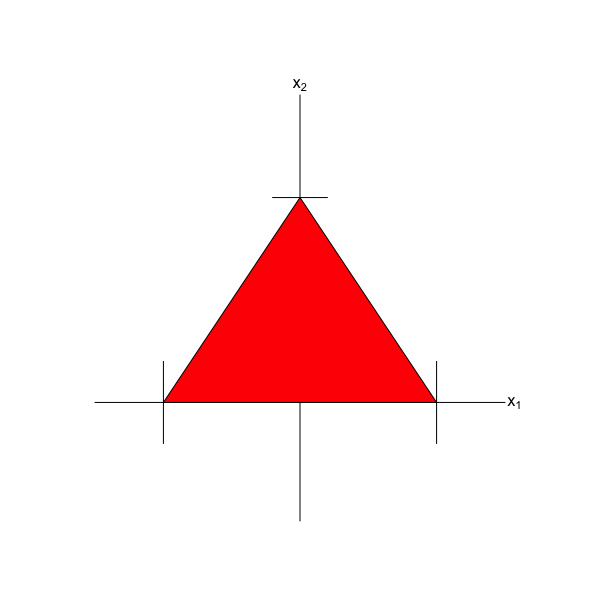
\includegraphics[width=0.75\linewidth,height=\textheight,keepaspectratio]{figures/multi_fig3.png}

}

\caption{\label{fig-mulfig3}The domain of the bivariate uniform
distribution with bounds 0 and 1 along each axis. The region
\(x_1 > 2x_2\) is indicated by the blue triangle.}

\end{figure}%

\subsubsection{Covariance of Multinomial Random
Variables}\label{covariance-of-multinomial-random-variables}

\begin{quote}
In Section~\ref{sec-chap3multi}, we introduce the multinomial
distribution, which governs experiments in which we sample data that can
\(m\) different discrete values. The probability mass function is \[
p_{X_1,\ldots,X_m}(x_1,\ldots,x_m \vert p_1,\ldots,p_m) = \frac{k!}{x_1! \cdots x_m!}p_1^{x_1}\cdots p_m^{x_m} \,,
\] where \(x_i\) represents the number of times outcome \(i\) is
observed in \(k\) trials, and where \(p_i\) is the probability of
observing outcome \(i\). As stated in Section~\ref{sec-chap3multi}, the
distribution for each random variable \(X_i\) is Binomial(\(k,p_i\)),
but the \(X_i\)'s are \emph{not} independent; because
\(\sum_{i=1}^m X_i = k\), increase the value of one of the random
variables would lead the values of the others to decrease on average.
Here we will derive the result that was quoted in
Section~\ref{sec-chap3multi}, namely that Cov(\(X_i\),\(X_j\)) =
\(-kp_ip_j\) for \(i \neq j\).
\end{quote}

\begin{quote}
Because \(X_i\) and \(X_j\) are each binomially distributed random
variables, we can view them as sums of Bernoulli distributed random
variables, i.e., we can write \[
X_i = \sum_{l=1}^k U_l ~~\mbox{and}~~ X_j = \sum_{l=1}^k V_l \,,
\] where \(U_l \sim\) Bernoulli(\(p_i\)) and \(V_l \sim\)
Bernoulli(\(p_j\)), and where \(l\) is an index representing the
\(l^{\mathrm{th}}\) trial.
\end{quote}

\begin{quote}
The covariance of \(X_i\) and \(X_j\) is thus \begin{align*}
\mbox{Cov}(X_i,X_j) &= E[X_iX_j] - E[X_i]E[X_j] \\
&= E[X_iX_j] - (k p_i)(k p_j) \\
&= E[X_iX_j] - k^2p_ip_j \,,
\end{align*} where \begin{align*}
E[X_iX_j] &= E[U_1V_1 + \cdots + U_1V_k + U_2V_1 + \cdots + U_2V_k + \cdots U_kV_1 + \cdots + U_kV_k] \\
&= E[U_1V_1] + E[U_1V_2] + \cdots + E[U_kV_k] \,.
\end{align*} There are \(k^2\) terms in this summation overall. Because
we cannot observe two different outcomes in the same trial,
\(E[U_iV_i] = 0\) for all indices \(i \in [1,k]\). As for the other
\(k^2 - k\) terms\ldots let's starting by looking at one of them: \[
E[U_1V_2] = E[U_1]E[V_2] = p_ip_j \,.
\] This result holds because the results of any two trials in a
multinomial experiment are independent random variables. Thus the sum of
the remaining \(k^2-k\) terms is \((k^2-k)p_ip_j\), and thus \[
\mbox{Cov}(X_i,X_j) = (k^2-k)p_ip_j - k^2p_ip_j = -kp_ip_j \,.
\]
\end{quote}

\subsubsection{Tying Covariance Back to Simple Linear
Regression}\label{tying-covariance-back-to-simple-linear-regression}

\begin{quote}
Above, we point out how \(R^2\) is related to the correlation
coefficient between the \(x_i\)'s and \(Y_i\)'s. Here, we extend that
discussion to the determinination of the correlation coefficient between
\(\hat{\beta}_0\) and \(\hat{\beta}_1\) in simple linear regression.
\end{quote}

\begin{quote}
When discussing simple linear regression in Section~\ref{sec-chap2slr},
we gave formulae for the variances of both \(V[\hat{\beta}_0]\) and
\(V[\hat{\beta}_1]\). However, now that we know about the concept of
covariance, we can ask a question that we did not ask then: are
\(\hat{\beta}_0\) and \(\hat{\beta}_1\) independent random variables?
The answer is: of course they are not; if we have a set of data that we
are trying to draw a line through, it should be intuitively obvious that
changing the intercept of the line will lead to its slope having to
change as well in order to (re-)optimize the sum of squared errors. So:
the covariance between \(\hat{\beta}_0\) and \(\hat{\beta}_1\) is
non-zero\ldots but how do we determine it?
\end{quote}

\begin{quote}
The standard method of determining covariance involves the calculation
of the so-called \emph{variance-covariance matrix}. (To be clear, this
is nomenclature that is specific to regression contexts.) Stated without
derivation or proof, that matrix is given by the following: \[
\boldsymbol{\Sigma} = \sigma^2 (\mathbf{X}^T\mathbf{X})^{-1} \,,
\] where \(\sigma^2\) is the true variance (which, as you will recall,
we assume does not vary as a function of \(x\)), \(\mathbf{X}\) is the
design matrix \[
\mathbf{X} = \left( \begin{array}{cc} 1 & x_1 \\ 1 & x_2 \\ \vdots & \vdots \\ 1 & x_n \end{array} \right) \,,
\] the superscript \(T\) denotes the matrix transpose, and where the
superscript \(-1\) denotes matrix inversion. The column of 1's in the
design matrix represents what we multiply \(\beta_0\) by in the model,
while the column of \(x_i\)'s represents what we multiply \(\beta_1\)
by. As far as \(\sigma^2\) is concerned\ldots we generally never know
this quantity, so we plug in \(\widehat{\sigma^2}\) in place of
\(\sigma^2\) above.
\end{quote}

\begin{quote}
Let's demonstrate how this works using the same data as we used to talk
through the output from the \texttt{R} function \texttt{lm()} in
Section~\ref{sec-chap2slr}.
\end{quote}

\begin{Shaded}
\begin{Highlighting}[]
\FunctionTok{set.seed}\NormalTok{(}\DecValTok{202}\NormalTok{)}
\NormalTok{x      }\OtherTok{\textless{}{-}} \FunctionTok{runif}\NormalTok{(}\DecValTok{40}\NormalTok{, }\AttributeTok{min =} \DecValTok{0}\NormalTok{, }\AttributeTok{max =} \DecValTok{10}\NormalTok{)}
\NormalTok{Y      }\OtherTok{\textless{}{-}} \DecValTok{4} \SpecialCharTok{+} \FloatTok{0.5} \SpecialCharTok{*}\NormalTok{ x }\SpecialCharTok{+} \FunctionTok{rnorm}\NormalTok{(}\DecValTok{40}\NormalTok{)}
\NormalTok{lm.out }\OtherTok{\textless{}{-}} \FunctionTok{lm}\NormalTok{(Y }\SpecialCharTok{\textasciitilde{}}\NormalTok{ x)}
\FunctionTok{summary}\NormalTok{(lm.out)}
\end{Highlighting}
\end{Shaded}

\begin{verbatim}

Call:
lm(formula = Y ~ x)

Residuals:
     Min       1Q   Median       3Q      Max 
-2.00437 -0.53068  0.04523  0.40338  2.47660 

Coefficients:
            Estimate Std. Error t value Pr(>|t|)    
(Intercept)   4.5231     0.3216  14.063  < 2e-16 ***
x             0.4605     0.0586   7.859 1.75e-09 ***
---
Signif. codes:  0 '***' 0.001 '**' 0.01 '*' 0.05 '.' 0.1 ' ' 1

Residual standard error: 0.9792 on 38 degrees of freedom
Multiple R-squared:  0.6191,    Adjusted R-squared:  0.609 
F-statistic: 61.76 on 1 and 38 DF,  p-value: 1.749e-09
\end{verbatim}

\begin{quote}
Recall that the estimate of \(\sigma\) is given by the
\texttt{Residual\ standard\ error}, which here is 0.9792, so
\(\widehat{\sigma^2} = 0.9587\). We can extract this from the object
\texttt{lm.out}:
\end{quote}

\begin{Shaded}
\begin{Highlighting}[]
\NormalTok{hat.sigma  }\OtherTok{\textless{}{-}} \FunctionTok{summary}\NormalTok{(lm.out)}\SpecialCharTok{$}\NormalTok{sigma}
\NormalTok{hat.sigma2 }\OtherTok{\textless{}{-}}\NormalTok{ hat.sigma}\SpecialCharTok{\^{}}\DecValTok{2}
\end{Highlighting}
\end{Shaded}

\begin{quote}
(To determine what quantities are available in an \texttt{R} list output
by a function such as \texttt{summary(lm)}, we can type
\texttt{names(summary(lm))}. Here, \texttt{names()} indicates that
\texttt{sigma} is an accessible list element.) We can set up the design
matrix as follows:
\end{quote}

\begin{Shaded}
\begin{Highlighting}[]
\NormalTok{X }\OtherTok{\textless{}{-}} \FunctionTok{cbind}\NormalTok{(}\FunctionTok{rep}\NormalTok{(}\DecValTok{1}\NormalTok{, }\DecValTok{40}\NormalTok{), x)}
\end{Highlighting}
\end{Shaded}

\begin{quote}
``cbind'' means ``column bind'': the first argument is a vector of 1's
that is bound to the second argument, which is the vector of \(x_i\)'s,
thus creating a matrix with 40 rows and 2 columns. We can now compute
the variance-covariance matrix:
\end{quote}

\begin{Shaded}
\begin{Highlighting}[]
\NormalTok{hat.sigma2 }\SpecialCharTok{*} \FunctionTok{solve}\NormalTok{(}\FunctionTok{t}\NormalTok{(X) }\SpecialCharTok{\%*\%}\NormalTok{ X)}
\end{Highlighting}
\end{Shaded}

\begin{verbatim}
                        x
   0.10344444 -0.01652116
x -0.01652116  0.00343436
\end{verbatim}

\begin{quote}
The function \texttt{t()} returns the transpose of \(X\) (a matrix with
2 rows and 40 columns), while \texttt{solve()} is the matrix inversion
function.
\end{quote}

\begin{quote}
What do we see above? First, if we take the square roots of the matrix
elements at upper left and lower right (i.e., along the matrix
diagonal), we get \[
se(\hat{\beta}_0) = \sqrt{0.1034} = 0.3216 ~~~ \mbox{and} ~~~ se(\hat{\beta}_0) = \sqrt{0.0034} = 0.0586 \,.
\] These quantities match the values in the \texttt{Std.\ Error} column
of the coefficient table output by \texttt{summary()}. Good! In
addition, however, we see the off-diagonal element \(-0.0165\): this is
Cov(\(\hat{\beta}_0,\hat{\beta}_1\)). The negative sign makes sense: if
we increase the intercept, we have to make the slope smaller (i.e., more
negative) to optimize that coefficient. The correlation is given by \[
\frac{\mbox{Cov}(\hat{\beta}_0,\hat{\beta}_1)}{se(\hat{\beta}_0) \cdot se(\hat{\beta}_1)} = \frac{-0.0165}{0.3216 \cdot 0.0586} = -0.8755 \,.
\] We see immediately that the intercept and slope are \emph{strongly}
(and negatively) correlated.
\end{quote}

\begin{quote}
In ``real-life'' situations, do we need to carry out the chain of
computations we carry out above? No\ldots because \texttt{R} provides
wrapper functions to help us:
\end{quote}

\begin{Shaded}
\begin{Highlighting}[]
\NormalTok{(Sigma }\OtherTok{\textless{}{-}} \FunctionTok{vcov}\NormalTok{(lm.out)) }\CommentTok{\# compute the variance{-}covariance matrix}
\end{Highlighting}
\end{Shaded}

\begin{verbatim}
            (Intercept)           x
(Intercept)  0.10344444 -0.01652116
x           -0.01652116  0.00343436
\end{verbatim}

\begin{Shaded}
\begin{Highlighting}[]
\FunctionTok{cov2cor}\NormalTok{(Sigma)          }\CommentTok{\# convert the covariance to correlation}
\end{Highlighting}
\end{Shaded}

\begin{verbatim}
            (Intercept)          x
(Intercept)   1.0000000 -0.8765245
x            -0.8765245  1.0000000
\end{verbatim}

\begin{quote}
(We note that the difference between the correlation coefficient
computed above and that output by \texttt{cov2cor()} is entirely due to
round-off error.)
\end{quote}

\subsubsection{Tying Covariance to Simple Logistic
Regression}\label{tying-covariance-to-simple-logistic-regression}

\begin{quote}
In the last example, we state that the variance-covariance matrix for
simple linear regression is given by \[
\boldsymbol{\Sigma} = \sigma^2 (\mathbf{X}^T\mathbf{X})^{-1} \,.
\] A similar expression exists for logistic regression: \[
\boldsymbol{\Sigma} = (\mathbf{X}^T \mathbf{W} \mathbf{X})^{-1} \,,
\] where the diagonal weight matrix \(\mathbf{W}\) is given by \[
\mathbf{W} = \left( \begin{array}{cccc} \frac{\exp(\hat{\beta}_0 + \hat{\beta}_1x_1)}{(1+\exp(\hat{\beta}_0 + \hat{\beta}_1x_1))^2} & 0 & \cdots & 0 \\ 0 & \frac{\exp(\hat{\beta}_0 + \hat{\beta}_1x_2)}{(1+\exp(\hat{\beta}_0 + \hat{\beta}_1x_2))^2} & \cdots & 0 \\ \vdots & \vdots & \ddots & \vdots \\ 0 & 0 & \cdots & \frac{\exp(\hat{\beta}_0 + \hat{\beta}_1x_n)}{(1+\exp(\hat{\beta}_0 + \hat{\beta}_1x_n))^2} \end{array} \right) \,.
\] Note that if we were to replace every non-zero matrix entry above
with \(1/\sigma^2\), we would recover the expression
\(\boldsymbol{\Sigma} = \sigma^2 (\mathbf{X}^T\mathbf{X})^{-1}\).
\end{quote}

\begin{quote}
Below, we show how to populate the \(\mathbf{W}\) matrix and use it to
determine the variance-covariance matrix.
\end{quote}

\begin{Shaded}
\begin{Highlighting}[]
\CommentTok{\# run simple logistic regression on training dataset}
\NormalTok{log.out }\OtherTok{\textless{}{-}} \FunctionTok{glm}\NormalTok{(class }\SpecialCharTok{\textasciitilde{}}\NormalTok{ col.iz, }\AttributeTok{data =}\NormalTok{ df.train, }\AttributeTok{family =}\NormalTok{ binomial)}
\FunctionTok{summary}\NormalTok{(log.out)}
\end{Highlighting}
\end{Shaded}

\begin{verbatim}

Call:
glm(formula = class ~ col.iz, family = binomial, data = df.train)

Coefficients:
            Estimate Std. Error z value Pr(>|z|)   
(Intercept)  0.16841    0.09265   1.818  0.06911 . 
col.iz      -0.96729    0.31051  -3.115  0.00184 **
---
Signif. codes:  0 '***' 0.001 '**' 0.01 '*' 0.05 '.' 0.1 ' ' 1

(Dispersion parameter for binomial family taken to be 1)

    Null deviance: 970.41  on 699  degrees of freedom
Residual deviance: 958.16  on 698  degrees of freedom
AIC: 962.16

Number of Fisher Scoring iterations: 4
\end{verbatim}

\begin{Shaded}
\begin{Highlighting}[]
\NormalTok{hat.beta0 }\OtherTok{\textless{}{-}}\NormalTok{ log.out}\SpecialCharTok{$}\NormalTok{coefficients[}\DecValTok{1}\NormalTok{]}
\NormalTok{hat.beta1 }\OtherTok{\textless{}{-}}\NormalTok{ log.out}\SpecialCharTok{$}\NormalTok{coefficients[}\DecValTok{2}\NormalTok{]}
\NormalTok{e         }\OtherTok{\textless{}{-}} \FunctionTok{exp}\NormalTok{(hat.beta0 }\SpecialCharTok{+}\NormalTok{ hat.beta1 }\SpecialCharTok{*}\NormalTok{ df.train}\SpecialCharTok{$}\NormalTok{col.iz)}
\NormalTok{W         }\OtherTok{\textless{}{-}} \FunctionTok{diag}\NormalTok{(e }\SpecialCharTok{/}\NormalTok{ (}\DecValTok{1} \SpecialCharTok{+}\NormalTok{ e)}\SpecialCharTok{\^{}}\DecValTok{2}\NormalTok{)}
\NormalTok{X         }\OtherTok{\textless{}{-}} \FunctionTok{cbind}\NormalTok{(}\FunctionTok{rep}\NormalTok{(}\DecValTok{1}\NormalTok{, }\FunctionTok{nrow}\NormalTok{(df.train)), df.train}\SpecialCharTok{$}\NormalTok{col.iz)}
\NormalTok{(Sigma    }\OtherTok{\textless{}{-}} \FunctionTok{solve}\NormalTok{(}\FunctionTok{t}\NormalTok{(X) }\SpecialCharTok{\%*\%}\NormalTok{ W }\SpecialCharTok{\%*\%}\NormalTok{ X))}
\end{Highlighting}
\end{Shaded}

\begin{verbatim}
             [,1]        [,2]
[1,]  0.008584293 -0.01635715
[2,] -0.016357147  0.09641920
\end{verbatim}

\begin{Shaded}
\begin{Highlighting}[]
\FunctionTok{sqrt}\NormalTok{(Sigma[}\DecValTok{1}\NormalTok{, }\DecValTok{1}\NormalTok{])}
\end{Highlighting}
\end{Shaded}

\begin{verbatim}
[1] 0.09265146
\end{verbatim}

\begin{Shaded}
\begin{Highlighting}[]
\FunctionTok{sqrt}\NormalTok{(Sigma[}\DecValTok{2}\NormalTok{, }\DecValTok{2}\NormalTok{])}
\end{Highlighting}
\end{Shaded}

\begin{verbatim}
[1] 0.3105144
\end{verbatim}

\begin{quote}
We see that the diagonal elements match the standard errors output by
the \texttt{summary()} function. We can find the correlation between
\(\hat{\beta}_0\) and \(\hat{\beta}_1\) by using the function
\texttt{cov2cor()}:
\end{quote}

\begin{Shaded}
\begin{Highlighting}[]
\FunctionTok{cov2cor}\NormalTok{(Sigma)}
\end{Highlighting}
\end{Shaded}

\begin{verbatim}
           [,1]       [,2]
[1,]  1.0000000 -0.5685564
[2,] -0.5685564  1.0000000
\end{verbatim}

\begin{quote}
The correlation is not as strong as we observed above in our simple
linear regression example, but in absolute terms we would still say that
\(\hat{\beta}_0\) and \(\hat{\beta}_1\) are strongly negatively
correlated.
\end{quote}

\section{Marginal and Conditional
Distributions}\label{sec-chap6marginal}

What to take away from this section:

\begin{itemize}
\item
  In a bivariate setting, a \emph{marginal distribution} is the
  distribution of the random variable \(X_1\) (or \(X_2\)), irrespective
  of the value of the other random variable.
\item
  In the same setting, a \emph{conditional distribution} is the
  distribution of the random variable \(X_1\) (or \(X_2\)) given
  specific conditions on the value of the other random variable.
\end{itemize}

Let's say that we perform an experiment where we sample a pair of random
variables \((X_1,X_2)\) from a bivariate distribution, where \(X_1\) and
\(X_2\) are dependent random variables. Despite doing this, we might
ultimately find that we are only interested in how \(X_1\) is
distributed, regardless of the sampled value of \(X_2\) (or vice-versa).
The distribution that we'd like to derive is dubbed a \emph{marginal
distribution}.

To compute the marginal distribution for \(X_1\) when given a bivariate
pdf \(f_{X_1,X_2}(x_1,x_2)\), we integrate over all values of \(x_2\):
\[
f_{X_1}(x_1) = \int_{x_2} f_{X_1,X_2}(x_1,x_2) dx_2 \,,
\] while for a bivariate pmf, we simply replace integration with
summation, e.g., \[
p_{X_1}(x_1) = \sum_{x_2} p_{X_1,X_2}(x_1,x_2) \,.
\] (If we are interested in computing the marginal distribution for
\(X_2\), we would simply swap the indices 1 and 2 above.) An important
thing to keep in mind is that \emph{a marginal pdf (or pmf) is a pdf (or
pmf)}, meaning that it is like any other pdf (or pmf): it is
non-negative and it integrates (or sums) to one, it has an expected
value and a standard deviation, etc.

A related, albeit narrower question to the one motivating the
computation of marginals is: what is the distribution of \(X_1\) when
\(X_2 = x_2\)? (It is narrower in the sense that for a marginal, we do
not care about the sampled value of \(X_2\), while here, we do.) This
distribution is dubbed a \emph{conditional distribution}, and it is
defined as follows: \[
f_{X_1 \vert X_2}(x_1 \vert x_2) = \frac{f_{X_1,X_2}(x_1,x_2)}{f_{X_2}(x_2)} \,.
\] For a bivariate pmf, the expression is similar. As was the case with
a marginal distribution, \emph{a conditional pdf (or pmf) is a pdf (or
pmf)}. One might notice immediately the similarity between this
expression and the one defining conditional probability in
Section~\ref{sec-chap1conditional}: \(p(A \vert B) = p(A \cap B)/p(B)\).
This is not coincidental. For marginals, the analogous probability
expression is \(p(A) = \sum_i p(A \vert B_i) p(B_i)\), i.e., the law of
total probability! If this is not immediately evident, note that we can
replace the \(f_{X_1,X_2}(x_1,x_2)\) in the marginal integral with
\(f_{X_1 \vert X_2}(x_1 \vert x_2) f_{X_2}(x_2)\). Then we can see how
\(x_1\) takes the place of \(A\) and \(x_2\) takes the places of
\(B_i\).)

Why do we divide by a marginal distribution when deriving a conditional
distribution? The answer is simple: if we do not, then there is no
guarantee that the conditional pdf or pmf will integrate or sum to one.
Finding the conditional distribution is akin to chopping through the
bivariate pdf at a particular value of \(x_1\) or \(x_2\), and tracing
the pdf along the chopped edge. This traced-out function will be
non-negative, but it will not necessarily integrate to one. The division
by the marginal acts to ``normalize'' the traced-out function, i.e., the
division raises or lowers it such that it subsequently will integrate to
one.

As a final note, we will mention that if \(X_1\) and \(X_2\) are
independent random variables, then, e.g.,

\begin{itemize}
\tightlist
\item
  \(f_{X_1,X_2}(x_1,x_2) = f_{X_1}(x_1) f_{X_2}(x_2)\); and
\item
  \(f_{X_1 \vert X_2}(x_1 \vert x_2) = f_{X_1}(x_1)\) and
  \(f_{X_2 \vert X_1}(x_2 \vert x_1) = f_{X_2}(x_2)\)
\end{itemize}

The first bullet point above shows the result that we look for when
establishing the independence of two random variables mathematically: we
compute the marginals for each variable, take the product of marginals,
and see if it matches the original bivariate function. However, this
conventional textbook approach to establishing independence is
unnecessary, as it is sufficient to examine the domain of the bivariate
function and to determine if we can factorize it into separate functions
of \(x_1\) and \(x_2\).

\subsection{Examples}\label{examples-49}

\subsubsection{Marginal and Conditional Distributions for a Bivariate
PMF}\label{marginal-and-conditional-distributions-for-a-bivariate-pmf}

\begin{quote}
Let \(X_1\) and \(X_2\) have the following joint probability mass
function \(p_{X_1,X_2}(x_1,x_2)\):
\end{quote}

{\def\LTcaptype{none} % do not increment counter
\begin{longtable}[]{@{}cccc@{}}
\toprule\noalign{}
\endhead
\bottomrule\noalign{}
\endlastfoot
& \(x_2 = 0\) & \(x_2 = 1\) & \(x_2 = 2\) \\
\(x_1 = 1\) & 0.20 & 0.30 & 0.00 \\
\(x_1 = 2\) & 0.40 & 0.00 & 0.10 \\
\end{longtable}
}

\begin{quote}
What is the marginal distribution \(p_{X_2}(x_2)\) and the conditional
distribution \(p_{X_1 \vert X_2}(x_1 \vert x_2)\)?
\end{quote}

\begin{quote}
When probability masses are involved, the marginal distribution is
derived by summing over an axis (here, \(x_1\)): \[
p_{X_2}(x_2) = \sum_{x_1} p_{X_1,X_2}(x_1,x_2) \,.
\] For this problem, the summation can be done by inspection, yielding
the following marginal distribution:
\end{quote}

{\def\LTcaptype{none} % do not increment counter
\begin{longtable}[]{@{}ccc@{}}
\toprule\noalign{}
\endhead
\bottomrule\noalign{}
\endlastfoot
\(x_2 = 0\) & \(x_2 = 1\) & \(x_2 = 2\) \\
0.60 & 0.30 & 0.10 \\
\end{longtable}
}

\begin{quote}
As stated in the text above, a marginal pmf is a pmf, meaning that for
instance the values sum to 1, and we can compute quantities like
\(E[X_2] = 0 \times 0.6 + 1 \times 0.3 + 2 \times 0.1 = 0.5\).
\end{quote}

\begin{quote}
As for the conditional distribution, we have the following expression \[
p_{X_1 \vert X_2}(x_1 \vert x_2) = \frac{p_{X_1,X_2}(x_1,x_2)}{p_{X_2}(x_2)} \,,
\] which in practice means we take the original bivariate table and
divide each row by the marginal for \(x_2\), if we are conditioning on
\(x_2\), or divide each column by the marginal for \(x_1\), if we are
conditioning on \(x_1\). Here, we condition on \(x_2\), so our result is
\end{quote}

{\def\LTcaptype{none} % do not increment counter
\begin{longtable}[]{@{}cccc@{}}
\toprule\noalign{}
\endhead
\bottomrule\noalign{}
\endlastfoot
& \(x_2 = 0\) & \(x_2 = 1\) & \(x_2 = 2\) \\
\(x_1 = 1\) & 0.20/0.60 = 0.33 & 0.30/0.30 = 1.00 & 0.00/0.10 = 0.00 \\
\(x_1 = 2\) & 0.40/0.60 = 0.67 & 0.00/0.30 = 0.00 & 0.10/0.10 = 1.00 \\
\end{longtable}
}

\begin{quote}
In such a table, the values in the individual columns all need to sum to
one: given some value of \(x_2\), we will with probability 1 sample a
value of \(x_1\). (As should be clear, if we condition on \(x_1\)
instead, we'd generate a table in which the values in each row would sum
to 1.)
\end{quote}

\subsubsection{Marginal and Conditional Distributions for a Bivariate
PDF}\label{marginal-and-conditional-distributions-for-a-bivariate-pdf}

\begin{quote}
Let \(X_1\) and \(X_2\) have the following joint probability density
function: \[
f_{X_1,X_2}(x_1,x_2) = 6(1-x_2) \,,
\] with \(0 \leq x_1 \leq x_2 \leq 1\). What is the marginal
distribution \(f_{X_1}(x_1)\)? What is the conditional distribution
\(f_{X_2 \vert X_l}(x_2 \vert x_1)\)?
\end{quote}

\begin{quote}
Refer back to Figure~\ref{fig-mulfig1}. The marginal distribution is
defined as a function of \(x_1\), so we integrate over
\(x_2\)\ldots which means that for any given value of \(x_1\), the
bounds of integration are \(x_1 = x_2\) to 1: \[
f_{X_1}(x_1) = \int_{x_1}^1 6(1-x_2) dx_2 \,.
\] Why is the lower bound \(x_1\) instead of \(x_2\)? They are
interchangable, but if we use \(x_2\), then our final result would not
be a function of \(x_1\)! In general, if we integrate along one axis,
the integral bounds should be expressed in terms of the other axis. To
continue: \begin{align*}
f_{X_1}(x_1) &= \int_{x_1}^1 6(1-x_2) dx_2 \\
&= 6 \left[ \int_{x_1}^1 dx_2 - \int_{x_1}^1 x_2 dx_2 \right] \\
&= 6 \left[ \left. x_2 \right|_{x_1}^1 - \left. \frac{x_2^2}{2} \right|_{x_1}^1 \right] \\
&= 6 \left[ 1 - x_1 - \left(\frac{1}{2}-\frac{x_1^2}{2} \right) \right] \\
&= 3 - 6x_1 + 3x_1^2 = 3(1-x_1)^2 \,,
\end{align*} for \(0 \leq x_1 \leq 1\). See Figure~\ref{fig-marcond}.
Given the functional form and domain, we can recognize this as a
Beta(1,3) distribution. (Such recognition is helpful if, for instance,
we were to ask for the expected value of \(X_1\). Rather than doing yet
another integral, we'd write that
\(E[X_1] = \alpha/(\alpha+\beta) = 1/4\).)
\end{quote}

\begin{quote}
As for the conditional distribution\ldots once we have the marginal,
this is easy to write down: \[
f_{X_2 \vert X_1}(x_2 \vert x_1) = \frac{f_{X_1,X_2}(x_1,x_2)}{f_{X_1}(x_1)} = \frac{6(1-x_2)}{3(1-x_1)^2} = \frac{2(1-x_2)}{(1-x_1)^2} \,.
\] Refering back to Figure~\ref{fig-mulfig1}, we note that this
conditional expression can only be non-zero along the line from
\(x_2 = x_1\) to 1. So the domain of this conditional distribution is
\(x_2 \vert x_1 \in [x_1,1]\). See Figure~\ref{fig-marcond}.
\end{quote}

\begin{figure}

\begin{minipage}[t]{0.50\linewidth}

\centering{

\pandocbounded{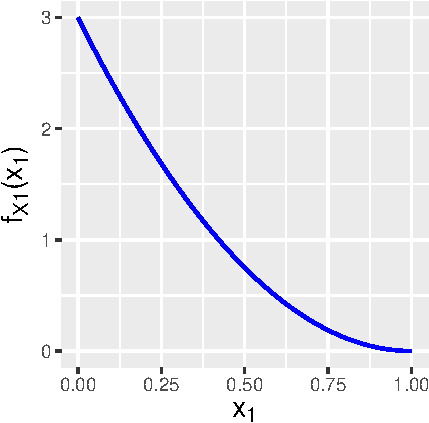
\includegraphics[keepaspectratio]{06-multivariate_files/figure-latex/fig-marcond-1.pdf}}

}

\subcaption{\label{fig-marcond-1}}

\end{minipage}%
%
\begin{minipage}[t]{0.50\linewidth}

\centering{

\pandocbounded{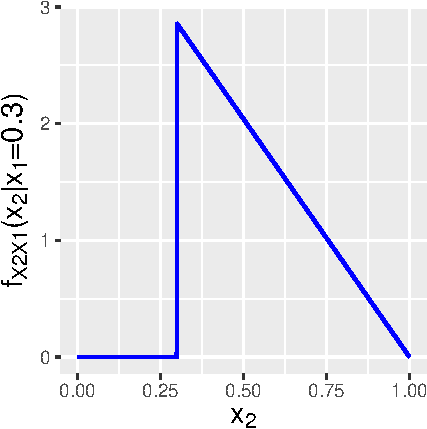
\includegraphics[keepaspectratio]{06-multivariate_files/figure-latex/fig-marcond-2.pdf}}

}

\subcaption{\label{fig-marcond-2}}

\end{minipage}%

\caption{\label{fig-marcond}The marginal distribution \(f_{X_1}(x_1)\)
and conditional distribution \(f_{X_2 \vert X_1}(x_2 \vert x_1=0.3)\)
for the bivariate function \(f_{X_1,X_2}(x_1,x_2) = 6(1-x_2)\) with
domain \(0 \leq x_1 \leq x_2 \leq 1\).}

\end{figure}%

\subsubsection{Mutual Information}\label{mutual-information}

\begin{quote}
Covariance and correlation are measures of \emph{linear} dependence. Is
there a conventional method for quantifying dependence more generally?
\end{quote}

\begin{quote}
Yes: the metric of \emph{mutual information}, which quantifies the
amount of information that one obtain about one random variable by
observing the other. The theoretical details of mutual information are
embedded within information theory and are thus beyond the scope of this
book, but we can easily write down, e.g., the mutual information held by
two continuously varying random variables \(X_1\) and \(X_2\):
\begin{align*}
I(X_1,X_2) = \int_{x_2} \int_{x_1} f_{X_1,X_2}(x_1,x_2) \log\left(\frac{f_{X_1,X_2}(x_1,x_2)}{f_{X_1}(x_1)f_{X_2}(x_2)}\right) dx_1 dx_2 \,.
\end{align*} In practice, the integration required to compute
\(I(X_1,X_2)\) can be difficult to carry out, but we can always fall
back upon numerical integration with the \texttt{integral2()} function
introduced in an example above. Let's suppose that our bivariate pdf is
the one in the previous example: \begin{align*}
f_{X_1,X_2}(x_1,x_2) &= 6(1-x_2) \\
f_{X_1}(x_1) &= 3(1-x_1)^2 \\
f_{X_2}(x_2) &= 6x_2(1-x_2) \,.
\end{align*} Then the mutual information is thus
\end{quote}

\begin{Shaded}
\begin{Highlighting}[]
\FunctionTok{library}\NormalTok{(pracma)}

\CommentTok{\# Define the (finite) domain}
\NormalTok{x1min }\OtherTok{\textless{}{-}} \DecValTok{0}
\NormalTok{x1max }\OtherTok{\textless{}{-}} \DecValTok{1} 
\NormalTok{x2min }\OtherTok{\textless{}{-}} \ControlFlowTok{function}\NormalTok{(x1) \{ x1 \} }\CommentTok{\# the lower bound for x2 is the line x2=x1}
\NormalTok{x2max }\OtherTok{\textless{}{-}} \DecValTok{1} 

\CommentTok{\# Determine I(X1, X2)}
\NormalTok{f }\OtherTok{\textless{}{-}} \ControlFlowTok{function}\NormalTok{(x1, x2) \{}
  \SpecialCharTok{{-}}\DecValTok{6} \SpecialCharTok{*}\NormalTok{ (}\DecValTok{1} \SpecialCharTok{{-}}\NormalTok{ x2) }\SpecialCharTok{*} \FunctionTok{log}\NormalTok{(}\DecValTok{3} \SpecialCharTok{*}\NormalTok{ x2 }\SpecialCharTok{*}\NormalTok{ (}\DecValTok{1}\SpecialCharTok{{-}}\NormalTok{x1)}\SpecialCharTok{\^{}}\DecValTok{2}\NormalTok{)}
\NormalTok{\} }
\NormalTok{I }\OtherTok{\textless{}{-}} \FunctionTok{integral2}\NormalTok{(f, x1min, x1max, x2min, x2max)}\SpecialCharTok{$}\NormalTok{Q}
\FunctionTok{cat}\NormalTok{(}\StringTok{"The value of I(X1, X2) is"}\NormalTok{, }\FunctionTok{round}\NormalTok{(I, }\DecValTok{3}\NormalTok{), }\StringTok{"}\SpecialCharTok{\textbackslash{}n}\StringTok{"}\NormalTok{)}
\end{Highlighting}
\end{Shaded}

\begin{verbatim}
The value of I(X1, X2) is 0.401 
\end{verbatim}

\begin{quote}
Unlike the correlation coefficient \(\rho_{X_1,X_2}\), a mutual
information value is not easily interpreted, beyond the fact that a
non-zero value indicates dependence. The interested reader can learn
more by examining how mutual information is tied to the individual,
conditional, and joint entropies of pairs of random variables.
\end{quote}

\section{Conditional Expected Value and
Variance}\label{sec-chap6conditional}

What to take away from this section:

\begin{itemize}
\item
  In a bivariate setting, the \emph{conditional expected value} and
  \emph{conditional variance} are the expected value of and variance of,
  e.g., \(X_1\) given a conditional distribution
  \(f_{X_1 \vert X_2}(x_1,x_2)\).
\item
  The laws to total expectation and of total variance allow us to derive
  unconditional expected values and variances given their conditional
  counterparts.
\end{itemize}

As was stated above, a conditional pdf or pmf is a pdf or
pmf\ldots meaning that like a pdf or pmf, it has an expected value and a
variance. For instance, the expected value of a conditional pdf
\(f_{X_1 \vert X_2}(x_1 \vert x_2)\), or the \emph{conditional expected
value}, is \[
E[X_1 \vert X_2] = \int_{x_1} x_1 f_{X_1 \vert X_2}(x_1 \vert x_2) dx_1 \,.
\] As you might expect, an analogous expression exists for bivariate
pmfs:
\(E[X_1 \vert X_2] = \sum_{x_1} p_{X_1 \vert X_2}(x_1 \vert x_2)\).
Also, there are two important points to make here:

\begin{itemize}
\tightlist
\item
  While, e.g., \(E[X_1]\) is a \emph{constant}, \(E[X_1 \vert X_2]\) is
  a \emph{random variable} due to the randomness of \(X_2\)\ldots that
  is, unless one specifies \(E[X_1 \vert X_2=x_2]\), which is constant
  because \(X_2\) is no longer random. Beware notation!
\item
  One can generalize \(E[X_1 \vert X_2]\) in the manner of the Law of
  the Unconscious Statistician:
  \(E[g(X_1) \vert X_2] = \int_{x_1} g(x_1) f_{X_1 \vert X_2}(x_1 \vert x_2) dx_1\).
\end{itemize}

The definition of \emph{conditional variance} builds off of that of the
conditional expected value: \begin{align*}
V[X_1 \vert X_2] &= E[(X_1-\mu_1)^2 \vert X_2] \\
&= E[X_1^2 \vert X_2] - (E[X_1 \vert X_2])^2 \\
&= \int_{x_1} x_1^2 f_{X_1 \vert X_2}(x_1 \vert x_2) dx_1 - \left[ \int_{x_1} x_1 f_{X_1 \vert X_2}(x_1 \vert x_2) dx_1 \right]^2 \,.
\end{align*} As we can see in the second line above, the fact that we
are dealing with a condition does not fundamentally change how variance
is computed: the form of the shortcut formula is the same as before,
just with the condition added.

Can one go from a conditional expected value to an unconditional
expected value \(E[X_1]\)? Yes: intuitively, this involves averaging the
values found for \(E[X_1 \vert X_2]\) over all possible values of
\(x_2\), weighting each of these possible values by how relatively
likely it is in the first place (i.e., in the case of a bivariate pdf,
weighting each value of \(E[X_1 \vert X_2]\) by \(f_{X_2}(x_2)\)):
\begin{align*}
E[X_1] = E[E[X_1 \vert X_2]] &= \int_{x_2} f_{X_2}(x_2) E[X_1 \vert X_2] dx_2 \\
&= \int_{x_2} f_{X_2}(x_2) \int_{x_1} x_1 f_{X_1 \vert X_2}(x_1 \vert x_2) dx_1 dx_2 \\
&= \int_{x_2} \int_{x_1} x_1 f_{X_2}(x_2) f_{X_1 \vert X_2}(x_1 \vert x_2) dx_1 dx_2 \\
&= \int_{x_1} \int_{x_2} x_1 f_{X_1,X_2}(x_1,x_2) dx_2 dx_1 = E[X_1] \,.
\end{align*}

As you might expect, given the conditional variance
\(V[X_1 \vert X_2]\), we can compute the unconditional variance
\(V[X_1]\)\ldots and for this, it is simplest to begin by writing down
that \[
V[X_1] = V[E[X_1 \vert X_2]] + E[V[X_1 \vert X_2]] \,.
\] The intuitive interpretation of this equation is that it reflects
that \(X_1\) can vary because the mean of \(X_1 \vert X_2\) can shift as
a function of \(X_2\) (so we want to quantify how much
\(E[X_1 \vert X_2]\) varies\ldots giving the first term on the right
above), but it can also vary due to being randomly distributed about the
mean (so we want to quantify how much, on average, is that random
variation\ldots which gives the second term above). As one might guess,
writing out the above expression in terms of integrals or summations
over bivariate functions is going to be messy and thus we forego doing
this here. (This might lead one to ask ``how will we solve unconditional
variance problems if expressions with integrals or summations are not
provided?'' It turns out there is an entire class of problems that we
can solve without integration or summation, and we provide an example of
a problem from that class below.)

Note that if \(X_1\) and \(X_2\) are independent, it follows that, e.g.,
\(E[X_1 \vert X_2] = E[X_1]\) and \(V[X_1 \vert X_2] = V[X_1]\). Let's
look at the latter expression. Above, we wrote that
\(V[X_1] = V[E[X_1 \vert X_2]] + E[V[X_1 \vert X_2]]\). If \(X_1\) and
\(X_2\) are independent, then \(E[X_1 \vert X_2]\) is a constant, and
thus \(V[E[X_1 \vert X_2]] = 0\) (because a constant does not vary). In
addition, \(V[X_1 \vert X_2]\) is a constant (it doesn't vary as \(X_2\)
changes) and thus \(E[V[X_1 \vert X_2]] = V[X_1 \vert X_2]\). So in the
end, \(V[X_1] = 0 + V[X_1 \vert X_2] = V[X_1 \vert X_2]\).

\subsection{Examples}\label{examples-50}

\subsubsection{Conditional and Unconditional Expected Value Given a
Bivariate
Distribution}\label{conditional-and-unconditional-expected-value-given-a-bivariate-distribution}

\begin{quote}
Let \(X_1\) and \(X_2\) have the following joint probability density
function: \[
f_{X_1,X_2}(x_1,x_2) = 6(1-x_2) \,,
\] with \(0 \leq x_1 \leq x_2 \leq 1\) (see Figure~\ref{fig-mulfig1}).
For this distribution, the marginal \(f_{X_2}(x_2)\) is \(6x_2(1-x_2)\)
for \(x_2 \in [0,1]\), or a Beta(2,2) distribution, while the
conditional distribution \(f_{X_1 \vert X_2}(x_1 \vert x_2)\) is \[
f_{X_1 \vert X_2}(x_1 \vert x_2) = \frac{f_{X_1,X_2}(x_1,x_2)}{f_{X_2}(x_2)} = \frac{6(1-x_2)}{6(1-x_2)x_2} = \frac{1}{x_2} \,,
\] for \(x_1 \in [0,x_2]\). (The interested reader can verify these
results!) What is \(E[X_1 \vert X_2]\) and what is \(E[X_1]\)?
\end{quote}

\begin{quote}
For the conditional expected value, we have that \begin{align*}
E[X_1 \vert X_2] &= \int_0^{x_2} x_1 f_{X_1 \vert X_2}(x_1 \vert x_2) dx_1 \\
&= \int_0^{x_2} \frac{x_1}{x_2} dx_1 \\
&= \frac{1}{x_2} \int_0^{x_2} x_1 dx_1 \\
&= \frac{1}{x_2} \left. \frac{x_1^2}{2} \right|_0^{x_2} = \frac{1}{x_2} \frac{x_2^2}{2} = \frac{x_2}{2} \,.
\end{align*} It turns out that we did not necessarily have to do this
integral, however. Note that the conditional expression is \(1/x_2\) for
\(x_1 \in [0,x_2]\)\ldots this is a uniform distribution! So we'd see,
by inspection, that the conditional expected value is \(x_2/2\).
\end{quote}

\begin{quote}
To determine the unconditional expected value \(E[X_1]\), we weight
every possible value of \(E[X_1 \vert X_2]\) by the probability
(density) that we would even observe \(X_2\) in the first place (which
is the marginal distribution for \(X_2\)): \begin{align*}
E[X_1] &= \int_0^1 f_{X_2}(x_2) E[X_1 \vert X_2] dx_2 \\
&= \int_0^1 6 x_2 (1 - x_2) \frac{x_2}{2} dx_2 \\
&= 3 \int_0^1 x_2^2 (1 - x_2) dx_2 \\
&= 3 B(3,2) = 3 \times 2! \times 1! / 4! = 1/4 \,.
\end{align*}
\end{quote}

\subsubsection{Conditional and Unconditional Expected Value and Variance
Given Two Univariate
Distributions}\label{conditional-and-unconditional-expected-value-and-variance-given-two-univariate-distributions}

\begin{quote}
Let's look at the following problem: the number of homework assignments
due in a given week, \(N\), varies from week to week and its value is
sampled from a Poisson distribution with mean \(\lambda\). The time to
complete any one homework assignment, \(X\), also varies, and its value
is sampled from a Gamma distribution with parameter \(\alpha\) and
\(\beta\) (and is the form of the Gamma with expected value
\(\alpha\beta\) and variance \(\alpha\beta^2\)). Let
\(T \vert N = \sum_{i=1}^N X_i\) be the total time spent completing
\(N\) homework assignments. (Assume all the \(X_i\)'s are independent
random variables.) What are \(E[T]\) and \(V[T]\)?
\end{quote}

\begin{quote}
We first note that because we are working with two univariate
distributions for which the expected value and variance are known, there
is no need to, e.g., integrate. We simply need to identify
\(E[T \vert N]\) and \(V[T \vert N]\) and work with those expressions
directly.
\end{quote}

\begin{quote}
We'll start with the expected value: \begin{align*}
E[T] &= E[E[T \vert N]] = E\left[E\left[\sum_{i=1}^N X_i\right]\right]\\
&= E\left[\sum_{i=1}^N E[X_i]\right] = E[N\alpha\beta] = \alpha \beta E[N] = \alpha\beta\lambda \,.
\end{align*} Somewhat more complicated is the computation of the
variance: \begin{align*}
V[T] &= V[E[T \vert N]] + E[V[T \vert N]] \\
&= V[N \alpha \beta] + E\left[ V \left[ \sum_{i=1}^N X_i \right] \right] \\
&= \alpha^2 \beta^2 V[N] + E \left[ \sum_{i=1}^N V[X_i] \right] \\
&= \alpha^2 \beta^2 \lambda + E \left[ \sum_{i=1}^N \alpha \beta^2 \right] \\
&= \alpha^2 \beta^2 \lambda + E[N\alpha \beta^2 ] \\
&= \alpha^2 \beta^2 \lambda + \alpha \beta^2 E[N] \\
&= \alpha^2 \beta^2 \lambda + \alpha \beta^2 \lambda = \alpha (\alpha + 1) \beta^2 \lambda \,.
\end{align*} Thus in any randomly chosen week, the time needed to
complete homework is \(\alpha\beta\lambda\) on average, with standard
deviation \(\sqrt{\alpha (\alpha + 1) \beta^2 \lambda}\).
\end{quote}

\section{The Multivariate Normal Distribution}\label{sec-chap6multnorm}

What to take away from this section:

\begin{itemize}
\item
  The \emph{multivariate normal distribution} is the multivariate
  analogue of the normal distribution, and it is parameterized by a mean
  vector \(\boldsymbol{\mu} = \{\mu_1,\ldots,\mu_p\}\) and a
  \emph{covariance matrix} \(\boldsymbol{\Sigma}\).
\item
  A \emph{marginal distribution} for a multivariate normal is derived by
  simply keeping the elements of the mean vector \(\boldsymbol{\mu}\),
  and the rows and columns of the covariance matrix
  \(\boldsymbol{\Sigma}\), that are associated with the axes we are
  retaining; the marginal is itself a multivariate normal.
\item
  A \emph{conditional distribution} for a multivariate normal is, like
  the marginal distribution, itself a multivariate normal, but with
  transformed mean vector \(\boldsymbol{\mu}\) and covariance matrix
  \(\boldsymbol{\Sigma}\).
\end{itemize}

The multivariate normal distribution is the most important one in
multivariate settings, due in part to its role in the multivariate
analogue of the central limit theorem: if we have a collection of \(n\)
iid random \emph{vectors}, where \(n\) is sufficiently large then the
sample mean vector is going to be approximately multivariate normally
distributed.

The joint probability density function for the multivariate normal is
given by \[
f_{\mathbf{X}}(\mathbf{x}) = \frac{1}{\sqrt{(2\pi)^p \vert \boldsymbol{\Sigma} \vert}} \exp\left(-\frac12 (\mathbf{x}-\boldsymbol{\mu})^T \boldsymbol{\Sigma}^{-1} (\mathbf{x}-\boldsymbol{\mu}) \right) \,.
\] Here, \(\mathbf{x} = \{x_1,\ldots,x_p\}\), and \(\boldsymbol{\mu} =
\{\mu_1,\ldots,\mu_p\}\) are the centroids of the normal along each of
the \(p\) coordinate axes. \(\boldsymbol{\Sigma}^{-1}\) is the inverse
of the covariance matrix \(\boldsymbol{\Sigma}\), while
\(\vert \boldsymbol{\Sigma} \vert\) is the determinant of
\(\boldsymbol{\Sigma}\). We denote sampling from this distribution with
the notation \[
\mathbf{X} \sim \mathcal{N}(\boldsymbol{\mu},\boldsymbol{\Sigma}) \,,
\] where \(\mathbf{X}\) is a \(p\)-dimensional vector.

\emph{To be clear: the multivariate normal is not a distribution that we
work with by hand!} We would conventionally use, e.g., \texttt{R} to do
any and all calculations.

That said, there are two qualitative facts about the multivariate normal
that are useful to know.

\begin{enumerate}
\def\labelenumi{\arabic{enumi}.}
\item
  A marginal distribution of the multivariate normal is itself a
  univariate or multivariate normal (depending on \(p\) and how many
  axes are being integrated over). To derive a marginal distribution,
  one simply needs to remove elements from the mean vector and from the
  covariance matrix. For instance, if \(p = 2\) and we wish to derive
  the marginal distribution for \(X_1\), then \begin{align*}
  \boldsymbol{\mu} &= [ \mu_1 ~ \mu_2 ] ~~\rightarrow \mu_{\mathrm{marg}} = \mu_1 \\
  \boldsymbol{\Sigma} &= \left( \begin{array}{cc} V[X_1] & \mbox{Cov}(X_1,X_2) \\ \mbox{Cov}(X_2,X_1) & V[X_2] \end{array} \right) ~~\rightarrow~~ \Sigma_{\mathrm{marg}} = V[X_1] \,.
  \end{align*} Here, we removed the second element of
  \(\boldsymbol{\mu}\) and the second row and second column of
  \(\boldsymbol{\Sigma}\). Note that \(\Sigma_{\mathrm{marg}}^{-1}\) is
  trivially \(1/V[X_1] = 1/\sigma_1^2\) and that the determinant of
  \(\Sigma_{\mathrm{marg}}\) is trivially \(V[X_1] = \sigma_1^2\).
  Plugging in these values, we can see that the marginal distribution
  for \(X_1\) has the form of a univariate normal pdf.
\item
  A conditional distribution of the multivariate normal is itself a
  univariate or multivariate normal (depending on \(p\) and how many
  axes are being conditioned upon). To derive a conditional
  distribution, we first identify which axes are being conditioned upon.
  Call that set of axes \(v\); all others we dub \(u\). (For instance,
  perhaps we want to determine the joint pdf of \(X_1\) and \(X_3\)
  given that we have set \(X_2 = x_2\) and \(X_4 = x_4\). Here,
  \(u = \{1,3\}\) and \(v = \{2,4\}\).) We split the mean vector and the
  covariance matrix into pieces: \begin{align*}
  \boldsymbol{\mu} &\rightarrow [ \boldsymbol{\mu}_u ~ \boldsymbol{\mu}_v ] \\
  \boldsymbol{\Sigma} &\rightarrow \left( \begin{array}{cc} \boldsymbol{\Sigma}_{uu} & \boldsymbol{\Sigma}_{uv} \\ \boldsymbol{\Sigma}_{vu} & \boldsymbol{\Sigma}_{vv} \end{array} \right) \,.
  \end{align*} (So, for instance,
  \(\boldsymbol{\mu}_v = [ \mu_2 ~ \mu_4 ]\), and \[
  \boldsymbol{\Sigma}_{uu} = \left( \begin{array}{cc} V[X_1] & \mbox{Cov}(X_1,X_3) \\ \mbox{Cov}(X_3,X_1) & V[X_3] \end{array} \right) \,,
  \] etc.) Given these pieces, we can define the conditional
  distribution \(\mathbf{X}_u \vert \mathbf{X}_v = \mathbf{x}_v\) as \[
  \mathbf{X}_u \vert \mathbf{X}_v = \mathbf{x}_v \sim \mathcal{N}(\boldsymbol{\mu}_c,\boldsymbol{\Sigma}_c) \,,
  \] where \begin{align*}
  \boldsymbol{\mu}_c &= \boldsymbol{\mu}_u + \boldsymbol{\Sigma}_{uv} \boldsymbol{\Sigma}_{vv}^{-1} (\mathbf{x}_v - \boldsymbol{\mu}_v) \\
  \boldsymbol{\Sigma}_c &= \boldsymbol{\Sigma}_{uu} - \boldsymbol{\Sigma}_{uv} \boldsymbol{\Sigma}_{vv}^{-1} \boldsymbol{\Sigma}_{vu} \,.
  \end{align*}
\end{enumerate}

\subsection{Examples}\label{examples-51}

\subsubsection{The Marginal Distribution of a Multivariate Normal
Distribution}\label{the-marginal-distribution-of-a-multivariate-normal-distribution}

\begin{quote}
Let's suppose that we have a three-dimensional normal distribution with
means \(\boldsymbol{\mu} = \{2,4,6\}\) and covariance matrix \[
\boldsymbol{\Sigma} = \left( \begin{array}{ccc} 2 & 0.5 & 1.2 \\ 0.5 & 2 & 1 \\ 1.2 & 1 & 2 \end{array} \right) \,.
\] What is the marginal distribution for \((X_1,X_2)\)?
\end{quote}

\begin{quote}
To determine the marginal distribution, we simply remove the third
element of \(\boldsymbol{\mu}\) and the third row and column of
\(\boldsymbol{\Sigma}\); the marginal distribution is a bivariate normal
with means \(\boldsymbol{\mu} = \{2,4\}\) and covariance matrix \[
\boldsymbol{\Sigma} = \left( \begin{array}{cc} 2 & 0.5 \\ 0.5 & 2 \end{array} \right) \,.
\]
\end{quote}

\begin{quote}
In \texttt{R}, we might visualize the result using the following code:
\end{quote}

\begin{verbatim}
     [,1] [,2] [,3]
[1,]  2.0  0.5  1.2
[2,]  0.5  2.0  1.0
[3,]  1.2  1.0  2.0
\end{verbatim}

\begin{verbatim}

Attaching package: 'metR'
\end{verbatim}

\begin{verbatim}
The following object is masked _by_ '.GlobalEnv':

    f
\end{verbatim}

\begin{verbatim}
The following object is masked from 'package:pracma':

    cross
\end{verbatim}

\begin{figure}

\centering{

\pandocbounded{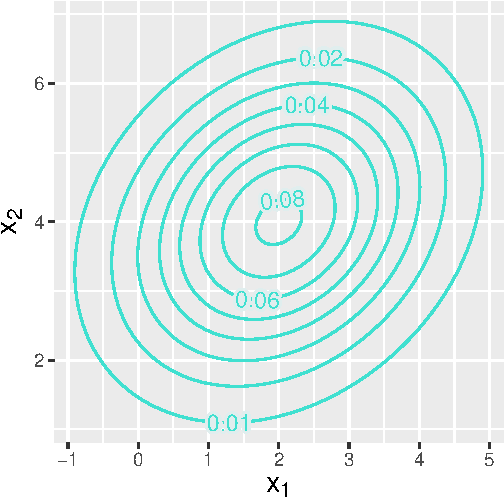
\includegraphics[keepaspectratio]{06-multivariate_files/figure-latex/fig-mvmarg-1.pdf}}

}

\caption{\label{fig-mvmarg}Contour plot indicating the location and
orientation of a bivariate normal distribution with mean
\(\boldsymbol{\mu} = \{2, 4\}\) and covariance matrix as given in the
example. The numbers along each contour indicate the amplitude of the
pdf, whose maximum point is in the center.}

\end{figure}%

\subsubsection{The Conditional Distribution of a Multivariate Normal
Distribution}\label{the-conditional-distribution-of-a-multivariate-normal-distribution}

\begin{quote}
Let's assume the same setting as in the previous example. What is the
conditional distribution of \(X_1\) and \(X_3\) given that \(X_2 = 5\)?
\end{quote}

\begin{quote}
Because of the complexity of the calculation, we will answer this
question using \texttt{R} code only, following the mathematical
prescription given in the text above.
\end{quote}

\begin{verbatim}
      [,1] [,2]
[1,] 1.875 0.95
[2,] 0.950 1.50
\end{verbatim}

\begin{figure}

\centering{

\pandocbounded{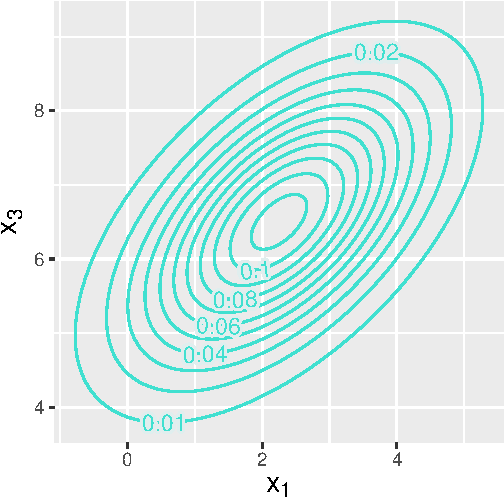
\includegraphics[keepaspectratio]{06-multivariate_files/figure-latex/fig-mvcond-1.pdf}}

}

\caption{\label{fig-mvcond}Contour plot indicating the location and
orientation of a bivariate normal distribution with conditional mean
\(\boldsymbol{\mu} = \{2.25, 6.50\}\) and conditional covariance matrix
as given in the example. The numbers along each contour indicate the
amplitude of the pdf, whose maximum point is in the center.}

\end{figure}%

\subsubsection{The Calculation of Sample
Covariance}\label{the-calculation-of-sample-covariance}

\begin{quote}
Let's assume that we observe \(n = 40\) iid data drawn from a bivariate
normal distribution with means \(\boldsymbol{\mu} = \{2,1\}\) and
covariance matrix \[
\boldsymbol{\Sigma} = \left( \begin{array}{cc} 1 & 0.5 \\ 0.5 & 2 \end{array} \right) \,.
\] Furthermore, we assume that the covariance matrix is unknown to us.
How would we estimate this matrix?
\end{quote}

\begin{verbatim}
      [,1]  [,2]
[1,] 1.798 1.704
[2,] 1.385 1.158
[3,] 2.551 2.707
\end{verbatim}

\begin{figure}

\centering{

\pandocbounded{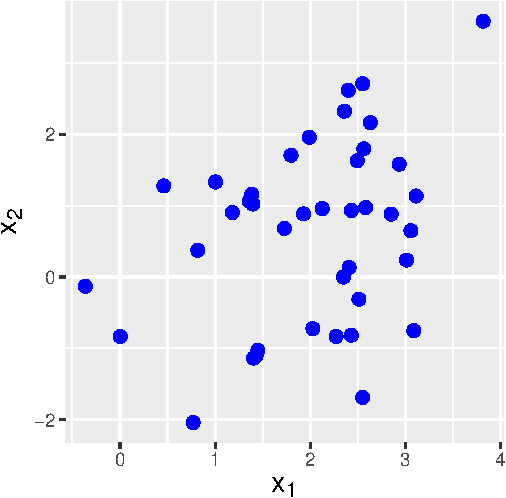
\includegraphics[keepaspectratio]{06-multivariate_files/figure-latex/fig-sampx-1.pdf}}

}

\caption{\label{fig-sampx}Sample of \(n = 40\) iid data drawn from a
bivariate normal distribution with means \(\boldsymbol{\mu} = \{2, 1\}\)
and covariance matrix \(\boldsymbol{\Sigma}\) given in the main body of
the text.}

\end{figure}%

\begin{quote}
First, let's sample some data. See Figure~\ref{fig-sampx}. The sample
covariance \(C_{jk}\) between variables \(j\) and \(k\) is given by \[
C_{jk} = \frac{1}{n-1} \sum_{i=1}^n (X_{ji} - \bar{X}_j)(X_{ki} - \bar{X}_k) \,.
\] So, for instance, for our data we would determine \(C_{12}\) in
\texttt{R} as follows:
\end{quote}

\begin{Shaded}
\begin{Highlighting}[]
\NormalTok{(}\DecValTok{1} \SpecialCharTok{/}\NormalTok{ (n }\SpecialCharTok{{-}} \DecValTok{1}\NormalTok{)) }\SpecialCharTok{*} \FunctionTok{sum}\NormalTok{((X[, }\DecValTok{1}\NormalTok{] }\SpecialCharTok{{-}} \FunctionTok{mean}\NormalTok{(X[, }\DecValTok{1}\NormalTok{])) }\SpecialCharTok{*}\NormalTok{ (X[, }\DecValTok{2}\NormalTok{] }\SpecialCharTok{{-}} \FunctionTok{mean}\NormalTok{(X[, }\DecValTok{2}\NormalTok{])))}
\end{Highlighting}
\end{Shaded}

\begin{verbatim}
[1] 0.389421
\end{verbatim}

\begin{quote}
This calculation matches that done by the \texttt{R} function
\texttt{cov()}:
\end{quote}

\begin{Shaded}
\begin{Highlighting}[]
\FunctionTok{cov}\NormalTok{(X)}
\end{Highlighting}
\end{Shaded}

\begin{verbatim}
          [,1]     [,2]
[1,] 0.8057418 0.389421
[2,] 0.3894210 1.653003
\end{verbatim}

\begin{quote}
The sample covariance matrix is an unbiased estimator of the true
covariance. We mention for completeness that just as the (scaled) sample
variance \((n-1)S^2/\sigma^2\) is chi-square-distributed for \(n-1\)
degrees of freedom, the sample covariance matrix is sampled from a
Wishart distribution, a multivariate generalization of the chi-square
distribution.
\end{quote}

\section{Exercises}\label{sec-chap6exercises}

\begin{enumerate}
\def\labelenumi{\arabic{enumi}.}
\item
  We are given the following bivariate pdf: \begin{align*}
  f_{X_1,X_2}(x_1,x_2) = \left\{ \begin{array}{cc} k(x_1+x_2^2) & 0 \leq x_1 \leq 1, 0 \leq x_2 \leq 1 \\ 0 & \mbox{otherwise} \end{array} \right. \,.
  \end{align*} (a) Determine the constant \(k\). (b) What is the
  conditional probability density function \(f_{X_1|X_2}(x_1|x_2)\)?
\item
  We are given the probability mass function shown below. (a) Compute
  Cov(\(X_1,X_2\)). (b) Compute \(\rho_{X_1,X_2}\). (c) Write down the
  conditional expected value \(E[X_1 \vert X_2 < 1]\). (This can be done
  by inspection.) (d) Write down the conditional variance
  \(V[X_2 \vert X_1 = 1]\). (This can also be done by inspection.)
\end{enumerate}

{\def\LTcaptype{none} % do not increment counter
\begin{longtable}[]{@{}ccc@{}}
\toprule\noalign{}
\endhead
\bottomrule\noalign{}
\endlastfoot
& \(x_1 = 0\) & \(x_1 = 1\) \\
\(x_2 = 0\) & 0.1 & 0.4 \\
\(x_2 = 1\) & 0.4 & 0.1 \\
\end{longtable}
}

\begin{enumerate}
\def\labelenumi{\arabic{enumi}.}
\setcounter{enumi}{2}
\item
  Every day, we sample \(n\) items built via an assembly line and look
  for defectives. On any given day, there is a constant probability
  \(p\) of assembling a defective item, but \(p\) can change from day to
  day: it is sampled from a Uniform(0,0.1) distribution. (a) What is the
  unconditional expected value for \(X\), the number of defectives
  observed per day? (Hint: what is the named distribution for the
  conditional expected value?) (b) What is the unconditional variance of
  \(X\)?
\item
  We are given the following bivariate probability density function:
  \begin{align*}
  f_{X_1,X_2}(x_1,x_2) = \left\{ \begin{array}{cl} k x_1^2 x_2 & x_1 \geq 0,\,x_2 \geq 0,\,x_1+x_2 \leq 1 \\ \\ 0 & \mbox{otherwise} \end{array} \right. \,.
  \end{align*} (a) Determine the value of \(k\) such that
  \(f_{X_1,X_2}(x_1,x_2)\) is a valid bivariate pdf. (b) Compute
  \(P(X_1 > 0.25 \vert X_2 = 0.5)\). (c) Are \(X_1\) and \(X_2\)
  independent random variables?
\item
  We are given the probability mass function shown below. (a) Write down
  the marginal probability mass function \(p_{X_2}(x_2)\). (b) Using our
  answer from (a), write down the marginal cdf \(F_{X_2}(x_2)\). (c)
  Assume \(p_X(x) = p_{X_2}(x_2)\) (i.e., forget the table
  exists\ldots all we have now is a univariate pmf). Compute the mean
  and standard deviation of \(p_X(x)\).
\end{enumerate}

{\def\LTcaptype{none} % do not increment counter
\begin{longtable}[]{@{}ccccc@{}}
\toprule\noalign{}
\endhead
\bottomrule\noalign{}
\endlastfoot
& & \(x_1 = 0\) & \(x_1 = 1\) & \(x_1 = 2\) \\
\(x_2 = 0\) & 0 & 0.2 & 0.1 & 0.1 \\
\(x_2 = 1\) & 1 & 0.1 & 0.3 & 0 \\
\(x_2 = 2\) & 2 & 0.05 & 0.05 & 0.1 \\
\end{longtable}
}

\begin{enumerate}
\def\labelenumi{\arabic{enumi}.}
\setcounter{enumi}{5}
\item
  We are given the following bivariate probability density function:
  \begin{align*}
  f_{X_1,X_2}(x_1,x_2) = \left\{ \begin{array}{cl} 60 x_1^2 x_2 & x_1 \geq 0,\,x_2 \geq 0,\,x_1+x_2 \leq 1 \\ \\ 0 & \mbox{otherwise} \end{array} \right. \,.
  \end{align*} We are also given that \(E[X_1] = 1/2\),
  \(E[X_2] = 1/3\), \(E[X_1^2] = 2/7\), and \(E[X_2^2] = 1/7\). (a)
  Compute Cov(\(X_1,X_2\)). (b) Compute Corr(\(X_1,X_2\)). (c) Compute
  \(V[X_1-2X_2]\).
\item
  The number of eggs laid by a certain insect is Poisson-distributed
  with mean \(\lambda\), and the probability that any one egg hatches is
  \(p\). Assume that the eggs hatch independently of one another. (a)
  Compute the expected value for the number of eggs that hatch. (b)
  Compute the variance for the number of eggs that hatch.
\item
  We are given the following bivariate probability density function:
  \begin{eqnarray*}
  f_{X_1,X_2}(x_1,x_2) = \left\{ \begin{array}{cc} k x_1 x_2 e^{-x_1/2} (1-x_2) & 0 \leq x_1 < \infty \,, \,0 \leq x_2 \leq 1 \\ 0 & \mbox{otherwise} \end{array} \right. \,.
  \end{eqnarray*} \(X_1\) and \(X_2\) are independent random variables.
  (a) What (numerical) value of \(k\) makes this a valid bivariate pdf?
  (b) Compute \(V[X_1-X_2]\).
\item
  We are given that the random variables \(X_1\) and \(X_2\) are
  distributed \emph{uniformly} within the region bounded by
  \(0 \leq x_2 \leq 1\) and \(0 \leq x_1 \leq 2-x_2\). (a) What is
  \(f_{X_1,X_2}(x_1,x_2)\) in the region specified above? For parts
  (b)-(d), assume \(f_{X_1,X_2}(x_1,x_2) = k\). (b) Write down the
  marginal distribution for \(X_2\). (c) Specify the conditional
  distribution for \(X_1\) given \(X_2 = x_2\). (d) What is the expected
  value of \(X_1\)? (e) Are \(X_1\) and \(X_2\) independent or dependent
  random variables?
\item
  A car drives through the same five traffic lights while on its way to
  work every day. The probability that the car has to stop at any given
  light on any given day is a beta-distributed random variable with
  parameters \(\alpha = \beta = 2\). (To be clear, the probability is
  \(p\) that the car will stop at the first light, then \(p\) that it
  will stop at the second light, etc., up to the fifth light. \(p\)
  changes from one day to the next.) Assume the traffic lights operate
  independently. (a) If \(X\) is the r.v. representing the number of
  lights the car stops at on any single day, what is \(E[X]\)? (b) What
  is \(V[X]\)?
\item
  We are given the following bivariate pdf: \begin{eqnarray*}
  f_{X_1,X_2}(x_1,x_2) = \left\{ \begin{array}{cc} 3x_1 & 0 \leq x_2 \leq x_1 \leq 1 \\ 0 & \mbox{otherwise} \end{array} \right. \,.
  \end{eqnarray*} We are also given that \(E[X_1]\) = 3/4, \(E[X_2]\) =
  3/8, \(V[X_1]\) = 3/80, and \(V[X_2]\) = 19/320. Compute the
  correlation coefficient \(\rho\) between \(X_1\) and \(X_2\).
\item
  We are given the following bivariate probability density function:
  \begin{eqnarray*}
  f_{X_1,X_2}(x_1,x_2) = \left\{ \begin{array}{cc} ke^{-x_1} & 0 \leq x_2 \leq x_1 < \infty \\ 0 & \mbox{otherwise} \end{array} \right. \,.
  \end{eqnarray*} (a) What value of \(k\) makes this a valid bivariate
  pdf? (b) What is \(P(X_2 < 1)\)? (c) Derive the marginal distribution
  for \(X_2\). (d) Derive the conditional pdf for \(X_1\) given
  \(X_2 = x_2\). (e) Compute \(P(X_1 > 2 \vert X_2 = 1)\).
\item
  A strangely designed prize machine works as follows: the payout \(X\),
  in dollars, is a Poisson-distributed random variable whose mean is
  sampled from a negative binomial distribution with \(r = 4\) and
  \(p = 1/2\). (a) Compute \(E[X]\). (b) Compute \(V[X]\).
\item
  We are given the following bivariate pdf: \begin{eqnarray*}
  f_{X_1,X_2}(x_1,x_2) = \left\{ \begin{array}{cc} c & -2 \leq x_1 \leq 2 \,, 0 \leq x_2 \leq \vert x_1 \vert \\ 0 & \mbox{otherwise} \end{array} \right. \,.
  \end{eqnarray*} (a) Are \(X_1\) and \(X_2\) independent random
  variables? (b) Determine \(c\). (c) Compute \(E[X_2]\).
\item
  We are given the following bivariate pdf: \begin{eqnarray*}
  f_{X_1,X_2}(x_1,x_2) = \left\{ \begin{array}{cc} cx_1x_2 & 0 \leq x_1 \leq 1 \,, 0 \leq x_2 \leq 1 \\ 0 & \mbox{otherwise} \end{array} \right. \,.
  \end{eqnarray*} (a) What is \(c\)? (b) What is
  \(P(X_2 > 1/2 \vert X_1 = 1/2)\)? (c) What is Cov(\(X_1,X_2\))?
\item
  We are given two r.v.'s, \(X_1\) and \(X_2\), whose variances are
  \(V[X_1] = V[X_2] = 3\) and whose covariance is 2. We define a new
  r.v. \(U = 2X_1 - X_2\). What is \(V[U]\)?
\item
  In an experiment, we flip a fair coin. If the coin shows heads, we
  then sample a datum \(U\) from a Uniform(1,2) distribution; otherwise
  we sample \(U\) from a Uniform(0,2) distribution. Compute the
  unconditional variance of the random variable \(U\).
\item
  We are given the following bivariate probability density function:
  \begin{eqnarray*}
  f_{X_1,X_2}(x_1,x_2) = \left\{ \begin{array}{cc} 12x_1^2(1-x_1) & 0 \leq x_1 \leq 1, 0 \leq x_2 \leq 1 \\ 0 & \mbox{otherwise} \end{array} \right. \,.
  \end{eqnarray*} (a) Are \(X_1\) and \(X_2\) independent random
  variables? (b) Write down the marginal distribution \(f_{X_2}(x_2)\).
  (c) Compute \(E[X_1]\).
\item
  We are given the following: \begin{eqnarray*}
  f_{X_1,X_2}(x_1,x_2) = \left\{ \begin{array}{cc} c & 0 \leq x_1 \leq 2, x_2 \geq 0, x_2 \leq x_1 ~\mbox{and}~x_2 \leq 2-x_1 \\ 0 & \mbox{otherwise} \end{array} \right. \,.
  \end{eqnarray*} (a) Determine the value of \(c\) that makes
  \(f_{X_1,X_2}(x_1,x_2)\) a valid pdf. (b) Write down the marginal
  distribution \(f_{X_2}(x_2)\). (c) Write down the conditional
  distribution \(f_{X_1 \vert X_2}(x_1 \vert x_2)\).
\item
  We are given the following bivariate probability density function:
  \begin{eqnarray*}
  f_{X_1,X_2}(x_1,x_2) = \left\{ \begin{array}{cc} 4x_1x_2 & 0 \leq x_1 \leq 1, 0 \leq x_2 \leq 1 \\ 0 & \mbox{otherwise} \end{array} \right. \,.
  \end{eqnarray*} (a) Compute \(f_{X_1}(x_1)\). (b) Compute
  \(f_{X_2 \vert X_1}(x_2 \vert x_1)\). (c) Compute
  \(P(X_2 < 1/2 \vert X_1=x_1)\).
\item
  We are given the following bivariate probability density function:
  \begin{eqnarray*}
  f_{X_1,X_2}(x_1,x_2) = \left\{ \begin{array}{cc} 2 & x_1 \geq 0~~x_2 \geq 0~~x_1+x_2 \leq 1 \\ 0 & \mbox{otherwise} \end{array} \right. \,.
  \end{eqnarray*} Compute the variance of \(X_1\).
\item
  We are given the probability mass function shown below. Compute the
  variance of \(X_1-X_2\). It may help to know that \(E[X_1^2] = 8/9\),
  \(E[X_2^2] = 6/9\), and \(E[X_1X_2] = 4/9\).
\end{enumerate}

{\def\LTcaptype{none} % do not increment counter
\begin{longtable}[]{@{}cccc@{}}
\toprule\noalign{}
\endhead
\bottomrule\noalign{}
\endlastfoot
& & \(x_2 = 0\) & \(x_2 = 1\) \\
\(x_1 = 0\) & 0 & 1/9 & 3/9 \\
\(x_1 = 1\) & 1 & 2/9 & 2/9 \\
\(x_1 = 2\) & 2 & 0 & 1/9 \\
\end{longtable}
}

\begin{enumerate}
\def\labelenumi{\arabic{enumi}.}
\setcounter{enumi}{22}
\item
  In an experiment, we sample a datum \(X\) from a gamma distribution
  whose \(\beta\) parameter is drawn from an exponential distribution
  with mean \(\gamma\). (a) What is the unconditional expected value of
  \(X\)? (b) What is \(V[X]\)?
\item
  We are given a bivariate uniform probability density function that is
  non-zero for \(0 \leq x_1 \leq 1\) and \(0 \leq x_2 \leq x_1\). (a)
  What is the amplitude of the pdf inside the region described above?
  (b) What is \(E[X_1]\)? (c) What is the covariance between \(X_1\) and
  \(X_2\)? (Note that \(E[X_2] = 1/3\).)
\item
  We are given the following bivariate probability density function:
  \begin{eqnarray*}
  f_{X_1,X_2}(x_1,x_2) = \left\{ \begin{array}{cc} k e^{-x_1/2} & x_1 \geq 0 ~{\mathrm{and}}~ 0 \leq x_2 \leq 2 \\ 0 & \mbox{otherwise} \end{array} \right. \,.
  \end{eqnarray*} (a) Find the value of \(k\) that makes
  \(f_{X_1,X_2}(x_1,x_2)\) a valid pdf. (b) Compute \(E[X_1]\).
\item
  We are given a bivariate uniform probability density function that is
  non-zero for \(x_2 \geq 0\), \(x_2 \leq x_1\), and \(x_2 \leq 2-x_1\).
  (a) Compute the marginal distribution for \(X_2\). (b) Compute the
  conditional distribution for \(X_1\) given \(X_2\). (c) Compute
  \(P(X_1 + X_2 \leq 1)\).
\item
  We sample a random variable \(X\) from a normal distribution with mean
  \(\mu\) and variance one, and you are given that \(\mu \sim N(0,1)\).
  Write down the variance of \(X\).
\item
  We are given the probability mass function shown below. (a) Compute
  the conditional expected value \(E[X_1 \vert X_2=1]\). (b) Compute the
  conditional variance \(V[X_1 \vert X_2=1]\).
\end{enumerate}

{\def\LTcaptype{none} % do not increment counter
\begin{longtable}[]{@{}ccc@{}}
\toprule\noalign{}
\endhead
\bottomrule\noalign{}
\endlastfoot
& \(x_2 = 0\) & \(x_2=1\) \\
\(x_1 = 0\) & 0.2 & 0.3 \\
\(x_1 = 1\) & 0.4 & 0.1 \\
\end{longtable}
}

\begin{enumerate}
\def\labelenumi{\arabic{enumi}.}
\setcounter{enumi}{28}
\item
  Let \(X_1\) and \(X_2\) be data that are jointly sampled from the
  bivariate probability density function \begin{eqnarray*}
  f_{X_1,X_2}(x_1,x_2) = k x_1^2 \,,
  \end{eqnarray*} where \(x_1 \geq 0\), \(x_2 \geq 0\), and
  \(x_1 + x_2 \leq 2\), and \(k\) is a constant. (a) Are \(X_1\) and
  \(X_2\) independent random variables? (b) What value of \(k\) makes
  \(f_{X_1,X_2}(x_1,x_2)\) a valid probability density function? (c)
  Derive the marginal distribution \(f_{X_1}(x_1)\). (d) Derive the
  conditional distribution \(f_{X_2 \vert X_1}(x_2 \vert x_1)\). (e)
  \(f_{X_2 \vert X_1}(x_2 \vert x_1)\) is a distribution from what named
  univariate family of distributions?
\item
  We are given the bivariate probability mass function shown below. (a)
  What is Cov(\(X_1,X_2\))? (b) What is \(\rho_{X_1,X_2}\)? (c) Let
  \(Y = 2X_1 - X_2\). Derive \(V[Y]\).
\end{enumerate}

{\def\LTcaptype{none} % do not increment counter
\begin{longtable}[]{@{}ccc@{}}
\toprule\noalign{}
\endhead
\bottomrule\noalign{}
\endlastfoot
& \(x_2 = 0\) & \(x_2 = 1\) \\
\(x_1 = 0\) & 0.3 & 0.1 \\
\(x_1 = 1\) & 0.1 & 0.5 \\
\end{longtable}
}

\bookmarksetup{startatroot}

\chapter{Additional Concepts (Optional)}\label{sec-chap7}

In this chapter, we provide information on concepts and results which
are just beyond the intended scope of this book, but which instructors
(and students!) might find useful regardless:

\begin{itemize}
\item
  convergence in probability versus convergence in distribution;
\item
  proofs of the central limit theorem and of the statement that maximum
  likelihood estimates are asymptotically normal;
\item
  the metric of efficiency for point estimators;
\item
  a deeper descent into the concept of sufficient statistics, including
  how one would determine whether a statistic is minimally sufficient
  and whether it is complete; and
\item
  a high-level discussion of how we would correct for multiple
  comparisons in hypothesis testing using either the Bonferroni
  correction or the Benjamini-Hochberg procedure (which controls the
  false-discovery rate).
\end{itemize}

\section{Types of Convergence}\label{sec-chap7convergence}

There are two primary types of convergence which are of interest to us
in this book: \emph{convergence in probability} and \emph{convergence in
distribution}.

Let \(X_1,X_2,\ldots\) be a sequence of random variables, and let \(Y\)
be some other random variable. (We note that the concept of a sequence
can be initially confusing for students: here, \(X_n\) is a statistic
formed from a set of data with sample size \(n\). A classic example of a
sequence is \(\bar{X}_1,\bar{X}_2,...\); the first element is the mean
for a sample of size 1 (the datum itself!), the second element is the
mean that we compute after we independently sample a second datum from
the same underlying distribution to go along with the first, etc.) In
addition, let \(F_{X_n}\) denote the cumulative distribution function
for \(X_n\) and \(F_Y\) denote the cdf for \(Y\). We say that

\begin{itemize}
\tightlist
\item
  \(X_n\) converges in probability to \(Y\) if for every
  \(\epsilon > 0\), \[
  P(\vert X_n - Y \vert > \epsilon) \rightarrow 0 
  \] as \(n \rightarrow \infty\); i.e.,
  \(X_n \overset{p}{\rightarrow} Y\).
\item
  \(X_n\) converges in distribution to \(Y\) if \[
  \lim_{n \rightarrow \infty} F_{X_n}(u) = F_Y(u) 
  \] for all values of \(u\) for which \(F_Y(u)\) is continuous; i.e.,
  \(X_n \overset{d}{\rightarrow} Y\).
\end{itemize}

An example of convergence in probability is the \emph{weak law of large
numbers}, which states that \(\bar{X}_n \overset{p}{\rightarrow} \mu\).
(This is a ``weak'' statement because it does not invoke ``almost sure''
convergence, a concept beyond the scope of this book.) What is ``weak''
about this statement? The statement
\(P(\vert \bar{X}_n - Y \vert > \epsilon) \rightarrow 0\), where \(Y\)
has mean \(\mu\), is not as restrictive a statement as others that one
can make; for any chosen value of \(\epsilon\),
\(\vert \bar{X}_n - Y \vert\) can stray so as to be greater than
\(\epsilon\) an infinite amount of times as \(n \rightarrow \infty\). In
other words, \(\bar{X}\) asymptotically approaches \(\mu\), but is still
``allowed'' to substantially deviate from that value for any finite
\(n\).

For more information on convergence concepts, see, e.g., Section 5.2 of
Wasserman (2004) or Section 5.5 of Casella and Berger (2002).

\section{The Central Limit Theorem: Proof}\label{sec-chap7cltproof}

We introduce the Central Limit Theorem in Section~\ref{sec-chap2clt}. It
states that if we have \(n\) iid random variables \(\{X_1,\ldots,X_n\}\)
with mean \(E[X_i] = \mu\) and finite variance
\(V[X_i] = \sigma^2 < \infty\), and if \(n\) is sufficiently large, then
\(\bar{X}\) converges in distribution to a standard normal random
variable: \[
\lim_{n \rightarrow \infty} P\left(\frac{\bar{X}-\mu}{\sigma/\sqrt{n}} \leq z \right) = \Phi(z) \,.
\] We can prove this using moment-generating functions.

Let \(X_i \overset{iid}{\sim} P(\mu,\sigma^2)\), where \(P\) is some
distribution with finite variance, and let \begin{align*}
Y &= \frac{\bar{X}-\mu}{\sigma/\sqrt{n}} = \frac{1}{\sqrt{n}} \left(\frac{n\bar{X} - n\mu}{\sigma}\right) = \frac{1}{\sqrt{n}} \left(\frac{\sum_{i=1}^n X_i - n\mu}{\sigma}\right)\\
&= \frac{1}{\sqrt{n}} \sum_{i=1}^n \frac{X_i - \mu}{\sigma} = \frac{1}{\sqrt{n}} \sum_{i=1}^n Z_i \,.
\end{align*} Since the \(Z_i\)'s are standardized random variables, by
definition \(E[Z_i] = 0\) and \(V[Z_i]\) = 1.

Here's where things ``break down'' if we do not know \(\sigma\), but
instead plug \(S\) in in CLT-related problems: if we use \(S\), then
\(V[X_i] \neq 1\). However, a theoretical result known as
\emph{Slutsky's theorem} saves us here. As we are determining here and
below, \[
\frac{\sqrt{n}(\bar{X} - \mu)}{\sigma} \overset{d}{\rightarrow} Z \sim \mathcal{N}(0,1) \,,
\] and hence \[
\sqrt{n}(\bar{X} - \mu) \overset{d}{\rightarrow} Y \sim \mathcal{N}(0,\sigma^2) \,.
\] Furthermore, \(S^2 \overset{p}{\rightarrow} \sigma^2\) (by the weak
law of large numbers), or equivalently
\(S \overset{p}{\rightarrow} \sigma\) (by the continuous mapping
theorem). Given these pieces of information, Slutsky's theorem tells us
that \(\sqrt{n}(\bar{X} - \mu)/S \overset{d}{\rightarrow} Y/\sigma\), a
normally distributed random variable with mean 0 and variance 1. Hence
eventually the CLT is valid, even when we plug in \(S\)!

To determine the distribution of \(Y\), we use the method of
moment-generating functions: \[
m_Y(t) = m_{Z_1}\left(\frac{t}{\sqrt{n}}\right) \cdots m_{Z_n}\left(\frac{t}{\sqrt{n}}\right) = \left[m_{Z_i}\left(\frac{t}{\sqrt{n}}\right)\right]^n \,.
\] ``Wait,'' one might say. ``We don't know the mgf for the quantity
\(Z_i\), so how can this possibly be helpful?'' It is because we can
work with the expected value and variance to get at the final result.
First, \begin{align*}
m_{Z_i}\left(\frac{t}{\sqrt{n}}\right) &= m_{Z_i}\left.\left(\frac{t}{\sqrt{n}}\right)\right|_{t=0} + m_{Z_i}'\left.\left(\frac{t}{\sqrt{n}}\right)\right|_{t=0} \frac{t}{\sqrt{n}} + m_{Z_i}''\left.\left(\frac{t}{\sqrt{n}}\right)\right|_{t=0} \frac{t^2}{2n} + \cdots \\
&\approx m_{Z_i}(0) + E[Z_i] \frac{t}{\sqrt{n}} + E[Z_i^2] \frac{t^2}{2n} \\
&= E[\exp(0Z_i)] + 0 + (V[Z_i] + (E[Z_i])^2) \frac{t^2}{2n} \\
&= 1 + V[Z_i] \frac{t^2}{2n} = 1 + \frac{t^2}{2n} \,.
\end{align*} Thus \[
m_Y(t) \approx \left[ 1 + \frac{t^2}{2n} \right]^n = \left[ 1 + \frac{t^2/2}{n} \right]^n \,,
\] and, as \(n \rightarrow \infty\), \[
\lim_{n \rightarrow \infty} \left[ 1 + \frac{t^2/2}{n} \right]^n = \exp\left(\frac{t^2}{2}\right) \,.
\] This is the moment-generating function for a standard
normal\ldots hence \(Y\) converges in distribution to a standard normal
random variable and \(\bar{X}\) converges in distribution to normal
random variable with mean \(\mu\) and variance \(\sigma^2/n\).

For more information on the Central Limit Theorem, see, e.g., Section
5.7.2 of Wasserman (2004), or Section 5.5.3 of Casella and Berger
(2002), where it is placed into the context of convergence in
distribution.

\section{Asymptotic Normality of Maximum Likelihood Estimates:
Proof}\label{sec-chap7asymmleproof}

When discussing point estimation in Section~\ref{sec-chap2point}, we
declared that as \(n \rightarrow \infty\), the maximum likelihood
estimate for a parameter \(\theta\) converges in distribution to a
normal random variable: \[
\sqrt{n}(\hat{\theta}_{MLE}-\theta) \overset{d}{\rightarrow} Y \sim \mathcal{N}\left(0,\frac{1}{I(\theta)}\right) ~\mbox{or}~ (\hat{\theta}_{MLE}-\theta) \overset{d}{\rightarrow} Y' \sim \mathcal{N}\left(0,\frac{1}{nI(\theta)}\right) \,.
\] Here, we sketch out why this is true. As we will see, this result
rests upon fundamental concepts covered earlier in this book and
chapter: the \hyperref[sec-chap7convergence]{weak law of large numbers}
(aka, convergence in probability), and the
\hyperref[sec-chap2clt]{central limit theorem}.

We start with the log-likelihood function
\(\ell(\theta \vert \mathbf{x})\). (However, to simplify the notation in
what follows, we will drop the \(\mathbf{x}\) for now.) By definition,
the MLE for \(\theta\) is that value for which \(\ell'(\theta) =
\ell'(\hat{\theta}_{MLE}) = 0\). The Taylor expansion of
\(\ell'(\theta)\) around \(\hat{\theta}_{MLE}\) is \[
\ell'(\theta) \approx \ell'(\hat{\theta}_{MLE}) + (\theta - \hat{\theta}_{MLE})\ell''(\theta) + \cdots = (\theta - \hat{\theta}_{MLE})\ell''(\theta) + \cdots \,.
\] We rearrange terms (and introduce the factor \(\sqrt{n}\)):
\begin{align*}
(\hat{\theta}_{MLE}-\theta)\ell''(\theta) &\approx -\ell'(\theta) \\
\sqrt{n} (\hat{\theta}_{MLE}-\theta)\ell''(\theta) &\approx -\sqrt{n}\ell'(\theta) \\
\sqrt{n} (\hat{\theta}_{MLE}-\theta) &\approx \frac{-\sqrt{n}\ell'(\theta)}{\ell''(\theta)} = \frac{\frac{1}{\sqrt{n}}\ell'(\theta)}{-\frac{1}{n}\ell''(\theta)} \,.
\end{align*} (Note that we reversed \(\theta\) and
\(\hat{\theta}_{MLE}\) in the parentheses!)

Let's look at the numerator and the denominator separately.

For the numerator: \begin{align*}
\frac{1}{\sqrt{n}}\ell'(\theta) &= \sqrt{n}\left(\frac{\ell'(\theta \vert \mathbf{x})}{n} - 0\right) \\
&= \sqrt{n}\left(\frac{\ell'(\theta \vert \mathbf{x})}{n} - E[\ell'(\theta \vert x_i)] \right) \\
&= \sqrt{n}\left(\frac{\sum_{i=1}^n \ell'(\theta \vert x_i)}{n} - E[\ell'(\theta \vert x_i)] \right) \,.
\end{align*} Here we utilize the results that, e.g.,
\(\ell'(\theta \vert \mathbf{x})\) equals the sum of the \(\ell'\)'s for
each datum, and that the average value of the slope for the likelihood
function is zero. What we have written is equivalent in form to \[
\sqrt{n} (\bar{X} - \mu)
\] and given the CLT, we know that as \(n \rightarrow \infty\), this
quantity converges in distribution to normal random variable
\(Y \sim \mathcal{N}(0,\sigma^2)\). Thus \[
\frac{1}{\sqrt{n}}\ell'(\theta) \overset{d}{\rightarrow} Y \sim \mathcal{N}\left(0,V[\ell'(\theta \vert x_i)]\right) \,,
\] and, since
\(V[\ell'(\theta \vert x_i)] = E[(\ell'(\theta \vert x_i))^2] - (E[\ell'(\theta \vert x_i)])^2 = E[(\ell'(\theta \vert x_i))^2] = I(\theta)\),
\[
\frac{1}{\sqrt{n}}\ell'(\theta) \overset{d}{\rightarrow} Y \sim \mathcal{N}\left(0,I(\theta)\right) \,.
\]

For the denominator, we can utilize the weak law of large numbers: \[
-\frac{1}{n} \ell''(\theta \vert \mathbf{x}) = -\frac{1}{n} \left( \sum_{i=1}^n \ell''(\theta \vert x_i) \right) \overset{p}{\rightarrow} -E[\ell''(\theta \vert x_i)] = I(\theta) \,.
\]

At last, we can determine the variance of the ratio: \begin{align*}
\lim_{n \rightarrow \infty} V[\sqrt{n}(\hat{\theta}_{MLE}-\theta)] &= V\left[ \frac{\frac{1}{\sqrt{n}}\ell'(\theta)}{I(\theta)} \right] = \frac{1}{I(\theta)^2} V\left[ \frac{1}{\sqrt{n}}\ell'(\theta) \right]\\
&= \frac{1}{I(\theta)^2} I(\theta) = \frac{1}{I(\theta)} \,.
\end{align*} We combine this information with the finding above that the
numerator in the ratio is, asymptotically, a normally distributed random
variable with mean 0 and variance \(I(\theta)\) to write \[
\sqrt{n}(\hat{\theta}_{MLE}-\theta) \overset{d}{\rightarrow} Y \sim \mathcal{N}\left(0,\frac{1}{I(\theta)}\right) \,.
\]

For more information regarding the asymptotic normality of maximum
likelihood estimates, see, e.g., Section 9.7 of Wasserman (2004), or
Theorem 10.1.12 of Casella and Berger (2002) and surrounding text.

\section{Point Estimation: (Relative)
Efficiency}\label{sec-chap7efficiency}

The efficiency of an unbiased estimator of a parameter \(\theta\) is \[
e(\hat{\theta}) = \frac{1/I(\theta)}{V[\hat{\theta}]} \,,
\] i.e., the ratio of the minimum possible variance for an unbiased
estimator of \(\theta\) (the Cramer-Rao lower bound) to the variance for
the estimator in question. If an unbiased estimator attains
\(e(\hat{\theta})\) for all possible values of \(\theta\), the estimator
is \emph{efficient}. (It is also the MVUE!)

The relative efficiency is a metric that we can use to compare two
unbiased estimators: \[
e(\hat{\theta}_1,\hat{\theta}_2) = \frac{V[\hat{\theta}_2]}{V[\hat{\theta}_1]} \,.
\] If \(e(\hat{\theta}_1,\hat{\theta}_2) > 1\), we would opt to use
\(\hat{\theta}_1\); otherwise, if
\(e(\hat{\theta}_1,\hat{\theta}_2) < 1\), we would opt to use
\(\hat{\theta}_2\). (We could use either if the relative efficiency is
exactly one.)

As an example, let \(X_i \sim \mathcal{N}(\mu,\sigma^2)\), and let
\(\hat{\mu}_1 =
\bar{X}\) and \(\hat{\mu}_2 = (X_1+X_2)/2\). What is the relative
efficiency of these two estimators?

We know the general result that \(V[\hat{\mu}_1] =
V[\bar{X}] = \sigma^2/n\), and we know that \(\hat{\mu}_2\) is simply
the sample mean of the first two data, so
\(V[\hat{\mu}_2] = V[(X_1+X_2)/2] = \sigma^2/2\). The relative
efficiency is thus \[
e(\hat{\mu}_1,\hat{\mu}_2) = \frac{V[\hat{\mu}_2]}{V[\hat{\mu}_1]} = \frac{\sigma^2/2}{\sigma^2/n} = \frac{n}{2} \,.
\] This value is \(> 1\) for all \(n > 2\), and it is never less than 1,
so we would choose to use \(\hat{\mu}_1 = \bar{X}\) as our estimator of
the population mean.

For more information about point estimation efficiency, see, e.g.,
Section 10.1.2 of Casella and Berger (2002).

\section{Sufficient Statistics: a Deeper Dive}\label{sec-chap7suffdeep}

Let us assume that we are given \(n\) independent and identically
distributed (iid) data sampled from some distribution \(P\) whose shape
is (without loss of generality) governed by a single parameter
\(\theta\): \[
\{X_1,\ldots,X_n\} \overset{iid}{\sim} P(\theta)
\] A sufficient statistic \(U\) is a function of \(\mathbf{X}\) that
encapsulates all the information needed to estimate \(\theta\), i.e., if
\(U\) is sufficient, no other computed statistic would provide any
additional information that would help us estimate \(\theta\).
Sufficient statistics are not unique: if \(U\) is a sufficient
statistic, then every one-to-one function \(f(U)\) is as well, so long
as \(f(U)\) does not depend on \(\theta\).

In Section~\ref{sec-chap3point} we show how one finds a sufficient
statistic by factorizing the likelihood function, and uses it to define
the minimum variance unbiased estimator (the MVUE). In our
demonstration, we sweep a number of things under the metaphorical rug,
such as the fact that to be used to determine the MVUE, a sufficient
statistic has to be both minimal and complete. We elaborate on those
points below. However, we start by providing an alternate means by which
to determine a sufficient statistic.

{[}For more information on the concept of sufficiency, see, e.g.,
Section 6.2 of Casella and Berger (2002); as for the Rao-Blackwell
theorem, see, e.g., Theorem 7.3.17 of the same text.{]}

\subsection{A Formal Definition of
Sufficiency}\label{sec-chap7suffformal}

A statistic \(U(\mathbf{X})\) is a sufficient statistic for the
parameter \(\theta\) if the conditional distribution of \(\mathbf{X}\)
given \(U(\mathbf{X})\) does not depend on \(\theta\), i.e., if
\(P(X_1=x_1,\ldots,X_n=x_n \vert U(\mathbf{X}) = k)\) does not depend on
\(\theta\).

As an example, let \(\{X_1,\ldots,X_n\} \overset{iid}{\sim}\)
Bernoulli(\(p\)), and let us propose
\(U(\mathbf{X}) = \sum_{i=1}^n X_i\) as a sufficient ststistic. To
determine if it is, we need to determine if \[
P(X_1=x_1,\ldots,X_n=x_n \vert U(\mathbf{X}=k) = \frac{P(X_1=x_1,\ldots,X_n=x_n,U(\mathbf{X})=k}{P(U(\mathbf{X}=k)}
\] does not depend on \(p\). The first thing to note is that for the
numerator to be non-zero, \(k = x_1+\cdots+x_n = \sum_{i=1}^n x_i\), and
thus \(U(\mathbf{Y})=k\) is, from an information standpoint,
\emph{completely redundant} with respect to
\(X_1=x_1,\ldots,X_n=x_n\)\ldots so we can ignore it: \[
P(X_1=x_1,\ldots,X_n=x_n \vert U(\mathbf{X}=k) = \frac{P(X_1=x_1,\ldots,X_n=x_n)}{P(U(\mathbf{X}=k)} \,.
\] The next thing to note is that because the data are iid, we can
rewrite the numerator as a product of probabilities: \[
P(X_1=x_1,\ldots,X_n=x_n) = P(X_1=x_1) \cdots P(X_n=x_n) = \prod_{i=1}^n P(X_i=x_i) \,,
\] which means, in the context of Bernoulli random variables, that the
numerator is \[
\prod_{i=1}^n P(X_i=x_i) = p^k (1-p)^{n-k} \,.
\] (Why \(p^k\), etc.? We are given that \(U(\mathbf{X}) = k\), i.e.,
that there are \(k\) observed successes (and \(n-k\) observed failures)
in the sample.

That takes care of the numerator. Now for the denominator: \[
P(U(\mathbf{X} = k) = \binom{n}{k} p^k (1-p)^{n-k} \,,
\] because the sum of \(n\) Bernoulli-distributed random variables is
binomially distributed (as you can show yourself using the method of
moment-generating functions).

Thus \[
P(X_1=x_1,\ldots,X_n=x_n \vert U(\mathbf{X}=k) = \frac{p^k(1-p)^{n-k}}{\binom{n}{k} p^k(1-p)^{n-k}} = \frac{1}{\binom{n}{k}} \,,
\] which does not depend on the parameter \(p\). Thus
\(U(\mathbf{X}) = \sum_{i=1}^n X_i\) is indeed a sufficient statistic
for \(p\).

(The foregoing clearly illustrates why factorization is a preferred
means by which to determine sufficient statistics!)

\subsection{Minimal Sufficiency}\label{sec-chap7suffminimal}

A question that naturally arises when dealing with sufficient statistics
is: if we have many sufficient statistics, which one is the best one? It
would be the one that ``reduces'' the data the most. In a given context,
\(U(\mathbf{X})\) is minimal sufficient if, given any another sufficient
statistic \(T(\mathbf{X})\), \(U(\mathbf{X}) = f(T(\mathbf{X}))\).

To generate a minimal sufficient statistic, one can make use of the
Lehmann-Scheffe theorem. If we have two iid samples of data of the same
size, \(\{X_1,\ldots,X_n\}\) and \(\{Y_1,\ldots,Y_n\}\), then, if the
ratio of likelihoods \[
\frac{\mathcal{L}(x_1,\ldots,x_n \vert \theta)}{\mathcal{L}(y_1,\ldots,y_n \vert \theta)}
\] is constant as a function of \(\theta\) if and only if
\(g(x_1,\ldots,x_n) =
g(y_1,\ldots,y_n)\) for a function \(g(\cdot)\), then
\(g(X_1,\ldots,X_n)\) is a minimal sufficient statistic for \(\theta\).

As an example, let \(\{X_1,\ldots,X_n\}\) and
\(\{Y_1,\ldots,Y_n\} \overset{iid}{\sim}\) Poisson(\(\lambda\)). The
ratio of likelihoods is \[
\frac{\mathcal{L}(x_1,\ldots,x_n \vert \theta)}{\mathcal{L}(y_1,\ldots,y_n \vert \theta)} = \frac{\prod_{i=1}^n \frac{\lambda^{x_i}}{x_i!} e^{-\lambda}}{\prod_{i=1}^n \frac{\lambda^{y_i}}{y_i!} e^{-\lambda}} = \frac{\prod_{i=1}^n \frac{1}{x_i!}}{\prod_{i=1}^n \frac{1}{y_i!}} \frac{\lambda^{\sum_{i=1}^n x_i}}{\lambda^{\sum_{i=1}^n y_i}} = \frac{\prod_{i=1}^n \frac{1}{x_i!}}{\prod_{i=1}^n \frac{1}{y_i!}} \lambda^{\left(\sum_{i=1}^n x_i - \sum_{i=1}^n y_i\right)} \,.
\] This is only constant as a function of \(\lambda\) if we can ``get
rid of'' \(\lambda\), by setting its exponent to 0\ldots i.e., by
setting \(\sum_{i=1}^n x_i = \sum_{i=1}^n y_i\). Thus \(g(\mathbf{x}) =
\sum_{i=1}^n x_i\) is a minimal sufficient statistic for \(\lambda\).

Note that in the context of the present course, any and all sufficient
statistics that we define via, e.g., factorization are minimal
sufficient.

One might ask ``what is an example of a sufficient statistic that is not
minimally sufficient?'' The answer is simple but may not initially be
intuitive, in that we naturally think of a statistic as being a single
number (the output from applying a given function to a full dataset).
However, e.g., a full dataset is a statistic, and it is a sufficient
statistic: there is sufficient information in a full dataset so as to
compute the likelihood of a population parameter \(\theta\). However, a
full dataset is not minimally sufficient! If
\(T(\mathbf{X}) = \bar{X}\), and \(U(\mathbf{X}) = \{X_1,\ldots,X_n\}\),
then we cannot define a function \(f\) such that
\(\{X_1,\ldots,X_n\} = f(\bar{X})\).

\subsection{Completeness}\label{sec-chap7suffcomplete}

The concept of the completeness of a statistic is a general concept,
i.e., it is not limited to sufficient statistics. One can think of it as
the idea that each value of \(\theta\) in a distribution maps to a
distinct pmf or pdf. We bring up completeness here because the concept
appears in the context of determining an MVUE: the sufficient statistic
that we find via, e.g., factorization technically needs to be both
minimal and complete.

Let \(f_U(u \vert \theta)\) be the family of pmfs or pdfs for the
statistic \(U(\mathbf{X})\). \(U\) is dubbed a \emph{complete} statistic
if \(E[g(U)] = 0\) for all \(\theta\) implies \(P(g(U) = 0) = 1\) for
all \(\theta\).

As an example, let \(U \sim\) Binomial(\(n,p\)), with \(0 < p < 1\), and
let \(g(\cdot)\) be a function such that \(E[g(U)] = 0\). Then \[
0 = E[g(U)] = \sum_{u=0}^n g(u) \binom{n}{u} p^u (1-p)^{n-u} = (1-p)^n \sum_{u=0}^n g(u) \binom{n}{u} \left( \frac{p}{1-p}\right)^u \,.
\] For any choice of \(u\) and \(n\), \(\binom{n}{u} [p/(1-p)]^u > 0\).
So, in order to have \(E[g(U)] = 0\) for all \(p\), \(g(u) = 0\) for all
\(u\), i.e., \(P(g(U) = 0) = 1\). Therefore \(U\) is a complete
statistic.

Note that a complete statistic is also minimal sufficient, but the
converse is not necessarily true: a minimal sufficient statistic may not
be complete.

\subsection{The Rao-Blackwell Theorem}\label{sec-chap7rao}

The Rao-Blackwell theorem implies that an unbiased estimator for
\(\theta\) with a small variance is, or can be made to be, a function of
a sufficient statistic: if we have an unbiased estimator for \(\theta\),
we might be able to improve it using the prescription of the theorem. In
the end, the theorem provides a mathematically more challenging route to
defining a minimum variance unbiased estimator than what we show in the
main text\(-\)likelihood factorization followed by the ``de-biasing'' of
a sufficient statistic\(-\)and hence we relegate it here.

Let \(\hat\theta\) be an unbiased estimator for \(\theta\) such that
\(V[\hat\theta] < \infty\). If \(U\) is a sufficient statistic for
\(\theta\), define \(\hat\theta^* = E[\hat\theta \vert U]\). Then, for
all \(\theta\), \[
E[\hat\theta^*] = \theta ~~~ \text{and} ~~~ V[\hat\theta^*] \leq V[\hat\theta] \,.
\]

Let's suppose we have sampled \(n\) iid data from a Binomial
distribution with number of trials \(k\) and proportion \(p\). We
propose an estimator for \(p\): \(X_1/k\). First, is \(\hat{p} = X_1/k\)
unbiased? We have that \[
E[\hat{p}-p] = E\left[\frac{X_1}{k}\right] - p = \frac{1}{k}E[X_1] - p = \frac{1}{k}kp - p = 0 \,.
\] So\ldots yes. Second, is \(V[\hat{p}] < \infty\)?
\(V[X_1/k] = V[X_1]/k^2 = p(1-p)/k\)\ldots so, also yes. We are thus
free to use the Rao-Blackwell theorem to improve upon
\(\hat{p} = X_1/k\): \[
\hat\theta^* = E[\hat\theta \vert U] = E\left[\frac{X_1}{k} \left| ~ U = \sum_{i=1}^n X_i \right. \right] \,.
\] Since we are given the sum of the data, and since the data are iid,
we would expect, on average, that \(X_1\) has the value \(U/n\), and
thus that \(X_1/k\) has the value \(U/(nk)\). Thus \[
\hat\theta^* = \frac{\bar{X}}{k}
\] is the MVUE for \(p\).

\section{Hypothesis Testing: Multiple
Comparisons}\label{sec-chap7multiple}

\emph{Multiple comparisons} is a somewhat opaque term that denotes the
situation in which we perform many hypothesis tests
\emph{simultaneously} and need to correct for the fact that if the null
is correct in all cases, it becomes more and more likely that we will
observe (multiple) instances in which we decide to reject the null. We
can illustrate this using the binomial distribution: if we collect \(k\)
sets of data (e.g., \(k\) separate sets of \(n\) iid data sampled from a
Uniform(0,\(\theta\)) distribution), and perform level-\(\alpha\)
hypothesis tests for each, then the number of tests results in which we
reject the null is \[
X \sim \mbox{Binom}(k,\alpha) \,,
\] The expected value of \(X\) is \(E[X] = k\alpha\), which increases
with \(k\). The \emph{family-wise error rate}, or \emph{FWER}, is the
probability that at least one test will result in a rejection when the
null is correct: \[
FWER = P(X > 0) = 1 - P(X = 0) = 1 - \binom{k}{x} \alpha^0 (1-\alpha)^k = 1 - (1-\alpha)^k \,.
\] For instance, if \(k = 10\) and \(\alpha = 0.05\), the family-wise
error rate is 0.401: for every 10 tests we perform, the probability of
erroneously rejecting one or more null hypotheses (i.e., detecting one
or more \emph{false positives}) is about 40 percent. This increase in
the FWER with \(k\) is not good, and is well-known to be associated with
a commonly seen data analysis issue dubbed \emph{data dredging} or
\emph{p-hacking}. \(p\)-hacking greatly increases the probability that
researchers will make incorrect claims about what their data say, and
worse yet, that they will publish papers purporting these claims.

To mitigate this issue, we can attempt to change the test level for
individual tests such that the overall FWER is reduced to \(\alpha\).
There are many procedures for how we might go about changing the test
level for individual tests, but the most commonly used one is the
\emph{Bonferroni correction}: \[
\alpha \rightarrow \frac{\alpha}{k} \,.
\] What is the FWER given this correction? Let's assume the null is
correct for all \(k\) tests. Then \[
FWER = P\left( p_1 \leq \frac{\alpha}{k} \cup \cdots \cup p_k \leq \frac{\alpha}{k} \right) = \sum_{i=1}^k P\left( p_i \leq \frac{\alpha}{k}\right) = \sum_{i=1}^k \frac{\alpha}{k} = \alpha \,.
\] This works! Except\ldots what happens if actually only \(k'\) out of
the \(k\) are actually true? The FWER becomes
\(k' \alpha / k \leq \alpha\). Thus when there are incorrect nulls
sprinkled into the mix, the FWER is too low\ldots which means that the
Bonferroni correction is unduly conservative. Using it will lead to us
possibly not detecting false nulls that we should have detected! We
illustrate this issue in an example below.

An alternative to the Bonferroni correction and related procedures is to
not focus upon the FWER, but to attempt to limit the \emph{false
discovery rate}, or \emph{FDR}, instead. The simplest and most often
used FDR-based procedure is the one of Benjamini and Hochberg (1995).

\begin{itemize}
\tightlist
\item
  compute all \(k\) \(p\)-values;
\item
  sort the \(p\)-values into ascending order:
  \(p_{(1)},\ldots,p_{(k)}\);
\item
  determine the largest value \(k'\) such that
  \(p_{(k')} \leq k' \alpha / k\); and
\item
  reject the null for all tests that map to \(p_{(1)},\ldots,p_{(k')}\).
\end{itemize}

In an example below, we illustrate the use of the BH procedure. To be
clear: \(\alpha\) here represents the proportion of rejected null
hypotheses that are actually correct. (``We reject the null 20 times.
Assuming \(\alpha = 0.05\), then we expect that we were right to reject
the null 19 times, and that we'd be mistaken once.'') This is different
from the FWER setting, where \(\alpha\) represents the probability of
erroneously rejecting one or more null hypotheses. (``We perform 100
independent tests. Assuming \(\alpha =
0.05\), we expect to erroneously reject the null five percent of the
time when the null is correct\ldots but we can say nothing about how
often we correctly reject the null.'') We can further illustrate this
point with the following table:

{\def\LTcaptype{none} % do not increment counter
\begin{longtable}[]{@{}rccc@{}}
\toprule\noalign{}
& Null Correct & Null False & Total \\
\midrule\noalign{}
\endhead
\bottomrule\noalign{}
\endlastfoot
Null Rejected & V & S & R \\
Fail to Reject & U & T & k-R \\
Total & k' & k-k' & k \\
\end{longtable}
}

The only observable random variable here is \(R\), the total number of
rejected null hypotheses. In the FDR procedure, we focus on the first
\emph{row}. We know that \[
E[V] = \alpha k' \leq \alpha k
\] and we know that \(V+S \leq k\), so \[
E\left[\frac{V}{V+S}\right] = E\left[\frac{V}{R}\right] \leq \frac{\alpha k'}{k} \leq \alpha \,.
\] The FWER procedure, on the other hand, focuses on the first
\emph{column}, with \[
E\left[\frac{V}{V+U}\right] = \frac{\alpha k'}{k'} = \alpha \,.
\]

For more information on the Bonferroni method and the concept of
false-discovery rate, see, e.g., sections 9.1.2 and 9.3.2 of Lehmann and
Romano (2022).

\subsection{Examples}\label{examples-52}

\subsubsection{An Illustration of Multiple Comparisons When Testing for
the Normal
Mean}\label{an-illustration-of-multiple-comparisons-when-testing-for-the-normal-mean}

\begin{quote}
In the code chunk below, we generate \(k = 100\) independent datasets of
size \(n = 40\); for \(k' = 80\) datasets, \(\mu = 0\), and for the
remainder, \(\mu = 0.5\). For simplicity, we assume \(\sigma^2\) is
known and is equal to one. For each dataset, we test the hypotheses
\(H_o : \mu = 0\) versus \(H_a : \mu > 0\).
\end{quote}

\begin{Shaded}
\begin{Highlighting}[]
\FunctionTok{set.seed}\NormalTok{(}\DecValTok{101}\NormalTok{)}

\NormalTok{n      }\OtherTok{\textless{}{-}} \DecValTok{40}
\NormalTok{k      }\OtherTok{\textless{}{-}} \DecValTok{100}
\NormalTok{k.p    }\OtherTok{\textless{}{-}} \DecValTok{80}
\NormalTok{mu     }\OtherTok{\textless{}{-}} \FunctionTok{c}\NormalTok{(}\FunctionTok{rep}\NormalTok{(}\DecValTok{0}\NormalTok{, k.p), }\FunctionTok{rep}\NormalTok{(}\FloatTok{0.5}\NormalTok{, k }\SpecialCharTok{{-}}\NormalTok{ k.p))}
\NormalTok{mu.o   }\OtherTok{\textless{}{-}} \DecValTok{0}
\NormalTok{sigma2 }\OtherTok{\textless{}{-}} \DecValTok{1}

\NormalTok{p      }\OtherTok{\textless{}{-}} \FunctionTok{rep}\NormalTok{(}\ConstantTok{NA}\NormalTok{, k)}
\ControlFlowTok{for}\NormalTok{ ( ii }\ControlFlowTok{in} \DecValTok{1}\SpecialCharTok{:}\NormalTok{k ) \{}
\NormalTok{  X     }\OtherTok{\textless{}{-}} \FunctionTok{rnorm}\NormalTok{(n, }\AttributeTok{mean =}\NormalTok{ mu[ii], }\AttributeTok{sd =}\NormalTok{ sigma2)}
\NormalTok{  p[ii] }\OtherTok{\textless{}{-}} \DecValTok{1} \SpecialCharTok{{-}} \FunctionTok{pnorm}\NormalTok{(}\FunctionTok{mean}\NormalTok{(X), }\AttributeTok{mean =}\NormalTok{ mu.o, }\AttributeTok{sd =} \FunctionTok{sqrt}\NormalTok{(sigma2 }\SpecialCharTok{/}\NormalTok{ n))}
\NormalTok{\}}
\end{Highlighting}
\end{Shaded}

\begin{quote}
Below, we try two separate corrections for multiple comparisons: the
Bonferroni correction (controlling FWER), and the Benjamini-Hochberg
procedure (controlling FDR).
\end{quote}

\begin{Shaded}
\begin{Highlighting}[]
\NormalTok{alpha }\OtherTok{\textless{}{-}} \FloatTok{0.05}

\FunctionTok{cat}\NormalTok{(}\StringTok{"The number of rejected null hypotheses for Bonferroni: "}\NormalTok{, }
    \FunctionTok{sum}\NormalTok{(p }\SpecialCharTok{\textless{}}\NormalTok{ alpha }\SpecialCharTok{/}\NormalTok{ k), }\StringTok{"}\SpecialCharTok{\textbackslash{}n}\StringTok{"}\NormalTok{)}
\end{Highlighting}
\end{Shaded}

\begin{verbatim}
The number of rejected null hypotheses for Bonferroni:  9 
\end{verbatim}

\begin{Shaded}
\begin{Highlighting}[]
\NormalTok{w }\OtherTok{\textless{}{-}} \FunctionTok{which}\NormalTok{(p }\SpecialCharTok{\textless{}}\NormalTok{ alpha }\SpecialCharTok{/}\NormalTok{ k)}
\FunctionTok{cat}\NormalTok{(}\StringTok{"The number of falsely rejected null hypotheses is:     "}\NormalTok{, }\FunctionTok{sum}\NormalTok{(w }\SpecialCharTok{\textless{}=}\NormalTok{ k.p), }\StringTok{"}\SpecialCharTok{\textbackslash{}n}\StringTok{"}\NormalTok{)}
\end{Highlighting}
\end{Shaded}

\begin{verbatim}
The number of falsely rejected null hypotheses is:      0 
\end{verbatim}

\begin{Shaded}
\begin{Highlighting}[]
\NormalTok{p.sort }\OtherTok{\textless{}{-}} \FunctionTok{sort}\NormalTok{(p)}
\FunctionTok{cat}\NormalTok{(}\StringTok{"The number of rejected null hypotheses for FDR:        "}\NormalTok{, }
    \FunctionTok{sum}\NormalTok{(p.sort }\SpecialCharTok{\textless{}}\NormalTok{ (}\DecValTok{1}\SpecialCharTok{:}\NormalTok{k) }\SpecialCharTok{*}\NormalTok{ alpha }\SpecialCharTok{/}\NormalTok{ k), }\StringTok{"}\SpecialCharTok{\textbackslash{}n}\StringTok{"}\NormalTok{)}
\end{Highlighting}
\end{Shaded}

\begin{verbatim}
The number of rejected null hypotheses for FDR:         17 
\end{verbatim}

\begin{Shaded}
\begin{Highlighting}[]
\NormalTok{p.rej }\OtherTok{\textless{}{-}}\NormalTok{ p.sort[p.sort }\SpecialCharTok{\textless{}}\NormalTok{ (}\DecValTok{1}\SpecialCharTok{:}\NormalTok{k) }\SpecialCharTok{*}\NormalTok{ alpha }\SpecialCharTok{/}\NormalTok{ k]}
\NormalTok{w }\OtherTok{\textless{}{-}}\NormalTok{ p }\SpecialCharTok{\%in\%}\NormalTok{ p.rej}
\NormalTok{w }\OtherTok{\textless{}{-}} \FunctionTok{which}\NormalTok{(w }\SpecialCharTok{==} \ConstantTok{TRUE}\NormalTok{)}
\FunctionTok{cat}\NormalTok{(}\StringTok{"The number of falsely rejected null hypotheses is:     "}\NormalTok{, }\FunctionTok{sum}\NormalTok{(w }\SpecialCharTok{\textless{}=}\NormalTok{ k.p), }\StringTok{"}\SpecialCharTok{\textbackslash{}n}\StringTok{"}\NormalTok{)}
\end{Highlighting}
\end{Shaded}

\begin{verbatim}
The number of falsely rejected null hypotheses is:      0 
\end{verbatim}

\begin{quote}
With the Bonferroni correction, we reject nine null hypotheses (with the
guarantee that there is, on average, a five percent chance that we
erroneously reject one or more of the true nulls\ldots here, we reject
no correct null hypotheses. See Figure~\ref{fig-mcs}.
\end{quote}

\begin{quote}
With the BH procedure, we reject 17 null hypotheses (with the guarantee
that on average, five percent of these 17 {[}meaning, effectively, 1{]}
is an erroneous rejection\ldots here, we reject no correct null
hypotheses).
\end{quote}

\begin{figure}

\centering{

\pandocbounded{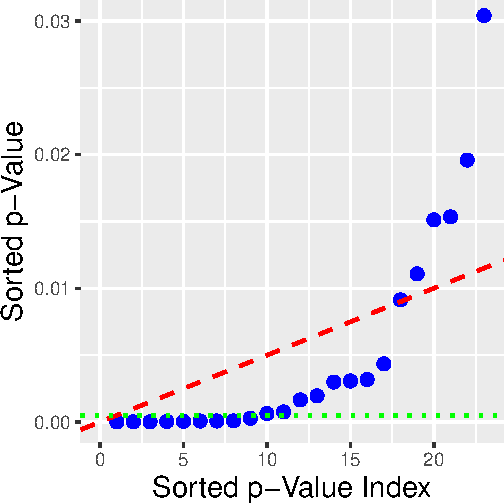
\includegraphics[keepaspectratio]{07-optional_files/figure-latex/fig-mcs-1.pdf}}

}

\caption{\label{fig-mcs}An illustration of the difference between the
Bonferroni correction and the Benjamini-Hochberg procedure. The blue
dots represent sorted \(p\)-values resulting from a simulation in which
80 of 100 null hypotheses are correct (so that a perfect disambiguation
between null and non-null hypotheses would result in 20 rejected nulls,
with none falsely rejected. The Bonferroni correction shifts
\(\alpha = 0.05\) downwards to the green short-dashed line; 9
\(p\)-values lie below the line, so 9 (true) null hypotheses are
rejected in all. The BH procedure looks for the number of \(p\)-values
lying below the red dashed line; that number is 17 (with no false
rejections).}

\end{figure}%

\bookmarksetup{startatroot}

\chapter*{Appendix: Table of Symbols}\label{appendix-table-of-symbols}
\addcontentsline{toc}{chapter}{Appendix: Table of Symbols}

\markboth{Appendix: Table of Symbols}{Appendix: Table of Symbols}

{\def\LTcaptype{none} % do not increment counter
\begin{longtable}[]{@{}
  >{\raggedright\arraybackslash}p{(\linewidth - 2\tabcolsep) * \real{0.1333}}
  >{\raggedright\arraybackslash}p{(\linewidth - 2\tabcolsep) * \real{0.8667}}@{}}
\toprule\noalign{}
\begin{minipage}[b]{\linewidth}\raggedright
Symbol
\end{minipage} & \begin{minipage}[b]{\linewidth}\raggedright
What the Symbol Represents
\end{minipage} \\
\midrule\noalign{}
\endhead
\bottomrule\noalign{}
\endlastfoot
\(\theta\) & parameter(s) that dictate the shape/location of a
distribution \\
\(\hat{\theta}\) & parameter estimate(s) \\
& \\
\(\alpha\) & one minus the confidence coefficient, or the hypothesis
test Type I error \\
\(\beta_i\) & the \(i^{\mathrm{th}}\) coefficient in a regression
model \\
\(\Gamma(x)\) & the gamma function \((= (x-1)!\) if \(x\) is an
integer) \\
\(\epsilon\) & the error term in a linear regression model \\
\(\mu\) & the distribution mean (or population mean) \((= E[X])\) \\
\(\mu_k'\) & the \(k^{\mathrm{th}}\) distribution moment
\((= E[X^k])\) \\
\(\nu\) & the number of degrees of freedom \\
\(\sigma\) & the distribution standard deviation (or population standard
deviation) \\
\(\sigma^2\) & the distribution variance (or population variance)
\((= V[X])\) \\
\(\boldsymbol{\Sigma}\) & the covariance matrix \\
\(\Omega\) & the sample space corresponding to an experiment \\
& \\
\(A\),\(B\) & generic symbols for events in a sample space \\
\(B(\alpha,\beta)\) & the beta function \\
\(B[\hat{\theta}]\) & the bias of the estimator \(\hat{\theta}\) \\
\(E[X]\) & the expected value of the random variable \(X\)
\((= \mu)\) \\
erf(\(x\)) & the error function \\
\(f_X(x)\) & the probability density function for the continuous random
variable \(X\) \\
\(F_X(x)\) & the cumulative distribution function for the random
variable \(X\) \\
iid & independent and identically distributed random variables \\
MSE & mean-squared error (\(V[\hat{\theta}] + B[\hat{\theta}]^2\)) \\
\(P(a \leq X \leq b)\) & the probability that \(X \in [a,b]\) \\
\(p_X(x)\) & the probability mass function for the discrete random
variable \(X\) \\
\(S\) & the standard deviation of \(n\) sampled data \\
\(S^2\) & the variance of \(n\) sampled data \\
\(T\) & a datum sampled from a \(t\) distribution \\
\(U\) & a sufficient statistic, found via likelihood factorization \\
\(V[X]\) & the variance of the random variable \(X\) \((= \sigma^2)\) \\
\(W\) & a datum sampled from a chi-square distribution \\
\(X\) & a single datum (or random variable), sampled from a pmf or
pdf \\
\(X_i\) & the \(i^{\mathrm{th}}\) datum of \(n\) sampled data \\
\(X_{(i)}\) & the \(i^{\mathrm{th}}\) smallest datum of \(n\) sampled
data \\
\(\bar{X}\) & the mean of \(n\) sample \\
\(Y\) & a statistic, a function of the data in a data sample \\
& \\
\(\mathcal{L}(\theta \vert \mathbf{x}\)) & the likelihood of \(\theta\)
given data coordinates \(\mathbf{x}\) \\
\(\ell(\theta \vert \mathbf{x}\)) & the log-likelihood
\(\log \mathcal{L}(\theta \vert \mathbf{x})\) \\
& \\
\(\cup\) & ``or'' in a probability statment \\
\(\cap\) & ``and'' in a probability statment \\
\(|\) & a condition, stated to the right of \(|\), in a probability
statement \\
\(\in\) & ``in,'' as in \(x \in [a,b]\) or ``\(x\) is in the range \(a\)
to \(b\)'' \\
& \\
\(\prod_{i=1}^n x_i\) & the product
\(x_1 \cdot x_2 \cdot \cdots \cdot x_n\) \\
\(\sum_{i=1}^n x_i\) & the summation
\(x_1 \cdot x_2 \cdot \cdots \cdot x_n\) \\
\end{longtable}
}

\bookmarksetup{startatroot}

\chapter*{Bibliography}\label{bibliography}
\addcontentsline{toc}{chapter}{Bibliography}

\markboth{Bibliography}{Bibliography}

\protect\phantomsection\label{refs}
\begin{CSLReferences}{1}{1}
\bibitem[\citeproctext]{ref-bh1995}
Benjamini, Y., and Y. Hochberg. 1995. {``Controlling the False Discovery
Rate: A Practical and Powerful Approach to Multiple Testing.''}
\emph{Journal of the Royal Statistical Society, Series B} 57: 289--300.

\bibitem[\citeproctext]{ref-bruner1976}
Bruner, J. S. 1976. \emph{{The Process of Education}}. Harvard
University Press, MA.

\bibitem[\citeproctext]{ref-buse1982}
Buse, A. 1982. {``The Likelihood Ratio, Wald, and Lagrange Multiplier
Tests: An Expository Note.''} \emph{The American Statistician} 36:
153--57.

\bibitem[\citeproctext]{ref-casella2002}
Casella, G., and R. L. Berger. 2002. \emph{Statistical Inference}. 2nd
ed. Duxbury Belmont, CA.

\bibitem[\citeproctext]{ref-efron1979}
Efron, B. 1979. {``Bootstrap Methods: Another Look at the Jackknife.''}
\emph{The Annals of Statistics} 7: 1--26.

\bibitem[\citeproctext]{ref-fisher1925}
Fisher, R. A. 1925. \emph{Statistical Methods for Research Workers}.
Oliver; Boyd Edinburgh, UK.

\bibitem[\citeproctext]{ref-freeman2026}
Freeman, P. E. 2026. {``Modernizing How Students Compute Interval
Estimates in Mathematical Statistics Courses.''} \emph{Journal of
Statistics and Data Science Education} 34: 450--63.

\bibitem[\citeproctext]{ref-hesterberg2015}
Hesterberg, T. 2015. {``What Teachers Should Know about the Bootstrap:
Resampling in the Undergraduate Statistics Curriculum.''} \emph{The
American Statistician} 69: 371--86.

\bibitem[\citeproctext]{ref-hogg2019}
Hogg, R. V, J. W. McKean, and A. T. Craig. 2019. \emph{Introduction to
Mathematical Statistics}. 8th ed. Pearson Boston, MA.

\bibitem[\citeproctext]{ref-james2021r}
James, G., D. Witten, T. Hastie, and R. Tibshirani. 2021. \emph{An
Introduction to Statistical Learning: With Applications in r}. 2nd ed.
Springer New York, NY.

\bibitem[\citeproctext]{ref-jamshidian2026}
Jamshidian, M., and P. Jamshidian. 2026. {``Unraveling the Mystery of
Equality in the Null Hypothesis: How Using Inequality Enhances
Conceptual Understanding of Hypothesis Testing for Our Introductory
Students.''} \emph{Journal of Statistics and Data Science Education} 34:
351--61.

\bibitem[\citeproctext]{ref-kolmogorov1933}
Kolmogorov, A. 1933. \emph{Grundbegriffe Der Wahrscheinlichkeitsrechnung
(Foundations of the Theory of Probability)}. Julius Springer Berlin,
Germany.

\bibitem[\citeproctext]{ref-lehmann2022}
Lehmann, E. L., and J. P. Romano. 2022. \emph{Testing Statistical
Hypotheses}. 4th ed. Springer New York, NY.

\bibitem[\citeproctext]{ref-pearson1900}
Pearson, K. 1900. {``On the Criterion That a Given System of Deviations
from the Probable in the Case of a Correlated System of Variables Is
Such That It Can Be Reasonably Supposed to Have Arisen from Random
Sampling.''} \emph{Philosophical Magazine} 50: 157--75.

\bibitem[\citeproctext]{ref-roback2021}
Roback, P., and J. Legler. 2021. \emph{Beyond Multiple Linear
Regression: Applied Generalized Linear Models and Multilevel Models in
r}. 1st ed. CRC Press Boca Raton, FL.

\bibitem[\citeproctext]{ref-ross1988}
Ross, S. 1988. \emph{A First Course in Probability}. 3rd ed. Macmillan
New York, NY.

\bibitem[\citeproctext]{ref-wasserman2004}
Wasserman, L. 2004. \emph{All of Statistics}. 1st ed. Springer New York,
NY.

\end{CSLReferences}

\bookmarksetup{startatroot}

\chapter*{Chapter Exercises:
Solutions}\label{chapter-exercises-solutions}
\addcontentsline{toc}{chapter}{Chapter Exercises: Solutions}

\markboth{Chapter Exercises: Solutions}{Chapter Exercises: Solutions}

\section*{Chapter 1}\label{chapter-1}
\addcontentsline{toc}{section}{Chapter 1}

\markright{Chapter 1}

\begin{itemize}
\tightlist
\item
  Problem 1
\end{itemize}

We start with Bayes' rule: \begin{align*}
P(A \vert B) &= \frac{P(B \vert A)P(A)}{P(B)} \\
\Rightarrow ~~~ \frac{P(B \vert A)P(A)}{P(B)} &= \frac{P(A \vert B)P(A)}{P(B)} \\
\Rightarrow ~~~ 1 &= \frac{P(A)}{P(B)} \\
\Rightarrow ~~~ P(A) &= P(B) \,.
\end{align*} Now let's look at a 2 \(\times\) 2 table:

{\def\LTcaptype{none} % do not increment counter
\begin{longtable}[]{@{}cccc@{}}
\toprule\noalign{}
\endhead
\bottomrule\noalign{}
\endlastfoot
& \(B\) & \(\bar{B}\) & \\
\(A\) & \(P(A \cap B)\) & \(P(A)-P(A \cap B)\) & \(P(A)\) \\
\(\bar{A}\) & \(P(A)-P(A \cap B)\) & 0.2 & \(1-P(A)\) \\
& \(P(A)\) & \(1-P(A)\) & \(1\) \\
\end{longtable}
}

So we have that \begin{align*}
P(A \cap B) + 2 [ P(A)-P(A \cap B) ] + 0.2 &= 1 \\
\Rightarrow ~~~ P(A \cap B) + 2 [ P(A)-P(A \cap B) ] &= 0.8 \\
\Rightarrow ~~~ 2 P(A) - P(A \cap B) &= 0.8 \\
\Rightarrow ~~~ P(A \cap B) &= 2 P(A) - 0.8 \,.
\end{align*}

\begin{center}\rule{0.5\linewidth}{0.5pt}\end{center}

\begin{itemize}
\tightlist
\item
  Problem 2
\end{itemize}

We are given that \(A \subset B\), so \begin{align*}
P(A \vert B)= \frac{P(B \cap A)}{P(B)} = \frac{P(A)}{P(B)} \neq P(A) \,.
\end{align*}

\begin{center}\rule{0.5\linewidth}{0.5pt}\end{center}

\begin{itemize}
\tightlist
\item
  Problem 3
\end{itemize}

We have that \begin{align*}
P(A \cap B| A\cup B)  = \frac{P[(A \cap B) \cap (A \cup B)]}{P(A\cup B)} = \frac{P(A \cap B)}{P(A\cup B)} = \frac{1 - P(\bar{A} \cup \bar{B})}{1 - P(\bar{A} \cap \bar{B})} \,.
\end{align*}

\begin{center}\rule{0.5\linewidth}{0.5pt}\end{center}

\begin{itemize}
\tightlist
\item
  Problem 4
\end{itemize}

(a) We have that \begin{align*}
P(B|A) + P(\bar{B}|A) &= 1 \\
\Rightarrow ~~~ P(B|A) &= \frac{1}{4} = \frac{1}{3}P(\bar{B}|A) \\
\Rightarrow ~~~ \frac{P(A \cap B)}{P(A)} &= \frac{1}{3} \frac{P(A \cap \bar{B})}{P[A]} \\ 
\Rightarrow ~~~ P(A \cap B) &= x = \frac{1}{3} \frac{1}{6} = \frac{1}{18} \,.
\end{align*}

(b) Here, we utilize a \(2 \times 2\) table:

{\def\LTcaptype{none} % do not increment counter
\begin{longtable}[]{@{}cccc@{}}
\toprule\noalign{}
\endhead
\bottomrule\noalign{}
\endlastfoot
& \(B\) & \(\bar{\text{B}}\) & \\
\(A\) & 1/18 & 1/6 & 4/18 \\
\(\bar{\text{A}}\) & & 1/3 & 14/18 \\
& 1/2 & 1/2 & \\
\end{longtable}
}

Thus \begin{align*}
p(\bar{A} \cap B) = \frac{14}{18} - \frac{6}{18} = \frac{8}{18}
\end{align*} and \begin{align*}
P(B|\bar{A}) = \frac{\bar{A} \cap B}{P(\bar{A})} = \frac{8/18}{14/18} = \frac{8}{14} = \frac{4}{7} \,.
\end{align*}

\begin{center}\rule{0.5\linewidth}{0.5pt}\end{center}

\begin{itemize}
\tightlist
\item
  Problem 5
\end{itemize}

One way to approach this problem is to write \begin{align*}
P(\bar{A}|\bar{B}) = \frac{P(\bar{A}\cap\bar{B})}{P(\bar{B})} = \frac{1 - P(A \cup B)}{1 - P(B)} \,;
\end{align*} equivalently, we can write \begin{align*}
P(\bar{A}|\bar{B}) = 1 - P(A|\bar{B}) =  1 - \frac{P(\bar{B}|A)P(A)}{P(\bar{B})} = 1 - \frac{\left[1 - P(B|A)\right]P(A)}{1 - P(B)} \,.
\end{align*}

\begin{center}\rule{0.5\linewidth}{0.5pt}\end{center}

\begin{itemize}
\tightlist
\item
  Problem 6
\end{itemize}

Using a decision tree:

\begin{itemize}
\tightlist
\item
  \(P(W_1) = 2/5\) and \(P(B_2 \vert W_1) = 3/4\), so
  \(P(B_2 \cap W_1) = 3/10\); and
\item
  \(P(B_1) = 3/5\) and \(P(B_2 \vert B_1) = 1/2\), so
  \(P(B_2 \cap B_1) = 3/10\).
\end{itemize}

Thus, by adding the probabilities of these disjoint events, we determine
that \(P(B_2) = P(B_2 \cap W_1) + P(B_2 \cap B_1) = 3/5\).

\begin{center}\rule{0.5\linewidth}{0.5pt}\end{center}

\begin{itemize}
\tightlist
\item
  Problem 7
\end{itemize}

If we denote the event of knowing the answer as \(K\), \(P(K) = 0.6\)
and \(P(\bar{K}) = 0.4\), and if we denote the event of getting the
question correct as \(C\), we know that \(P(C \vert \bar{K}) = 0.2\). It
is implicit in the wording of the question that \(P(C \vert K) = 1\).
Ultimately, we want to determine \(P(K \vert C)\): \begin{align*}
P(K \vert C) = \frac{P(C \vert K)P(K)}{P(C)} = \frac{P(C \vert K)P(K)}{P(C \vert K)P(K)+P(C \vert \bar{K})P(\bar{K})}  = \frac{1 \cdot 0.6}{1 \cdot 0.6 + 0.2 \cdot 0.4} = \frac{60}{68} = \frac{15}{17} \,.
\end{align*}

\begin{center}\rule{0.5\linewidth}{0.5pt}\end{center}

\begin{itemize}
\tightlist
\item
  Problem 8
\end{itemize}

We are given that \(P(S) = 0.15\),
\(P(D \vert S) = 10 \cdot P(D \vert \bar{S})\), and \(P(D) = 0.01\). So
\begin{align*}
P(S \vert D) &= \frac{P(D\vert S)P(S)}{P(D)} = \frac{P(D \vert S)P(S)}{P(D \vert S)P(S) + P(D \vert \bar{S})P(\bar{S})} \\
&= \frac{P(D \vert S)P(S)}{P(D \vert S)P(S) + P(D \vert S)(1 - P(S))/10} \\
&= \frac{P(S)}{P(S)+1/10-P(S)/10} = \cdots = 30/47 \,.
\end{align*}

\begin{center}\rule{0.5\linewidth}{0.5pt}\end{center}

\begin{itemize}
\tightlist
\item
  Problem 9
\end{itemize}

The compound event of winning is
\(W = \{ 1\cap3, 1\cap1\cap2, 1\cap1\cap3, \ldots \}\). Let the event
\(S\) denote rolling a 1, with \(P(S) = 1/3\), and the event \(F\)
denote rolling a 2 or a 3, with \(P(F) = 2/3\). Then \begin{align*}
P(W) &= P(1\cap3) + P(1\cap1\cap2) + \ldots = \\
&= \frac{1}{2} P(S) P(F) + P(S)^2 P(F) +  P(S)^3 P(F) + \ldots \\
&= \frac{1}{2}\frac{1}{3}\frac{2}{3} +  P(S)^2 P(F) \left(1 + P(S) + \ldots \right)\\
& = \frac{1}{9} + P(S)^2 P(F) \frac{1}{1 - P(S)} = \frac{1}{9} + \frac{P(S)^2 P(F) }{P(F)} = \frac{1}{9} + P(S^2) = \frac{2}{9} \,.
\end{align*} Alternatively, we can define compound event of losing,
\(L = \{2, 3, 1\cap2 \}\), and write that \begin{align*}
P(L) &= \frac{1}{3} + \frac{1}{3} + \left(\frac{1}{3}\right)^2 = \frac{7}{9} \\
\Rightarrow ~~~ P(W) &= 1 - P(L) = 1 - \frac{7}{9} = \frac{2}{9} \,.
\end{align*}

\begin{center}\rule{0.5\linewidth}{0.5pt}\end{center}

\begin{itemize}
\tightlist
\item
  Problem 10
\end{itemize}

There are multiple ways to do this. Here is one: \begin{align*}
P(H_1 \cup T_2) &= P(H_1) + P(T_2) - P(H_1 \cap T_2) = P(H_1) + P(T_2) - P(T_2 | H_1) P(H_1)\\
&= P(H_1) + P(T_2|H_1)P(H_1) + P(T_2|T_1)P(T_1) - P(T_2 | H_1) P(H_1)\\
&= P(H_1) + P(T_2|T_1)P(T_1) = 0.5 + 0.4 \cdot 0.5 = 0.7 \,.
\end{align*} Note: \(P(T_2|T_1) = 1 - P(H_2|T_1)= 0.4\), since \(H_2\)
is just \(\bar{T}_2\).

\begin{center}\rule{0.5\linewidth}{0.5pt}\end{center}

\begin{itemize}
\tightlist
\item
  Problem 11
\end{itemize}

Let \(N\) be the event that a sample contains nitrates and \(R\) be the
event that the sample burns red. We are given that \(P(N) = 0.2\),
\(P(R|N) = 0.9\), and \(P(R|\bar{N}) = 0.15\).

(a) We seek \(P(R)\), which is \begin{align*}
P(R|N)P(N) + P(R|\bar{N})P(\bar{N}) = 0.9 \cdot 0.2 + 0.15 \cdot (1-0.2) = 0.30 \,.
\end{align*}

(b) We seek \(P(N|R)\), which is \begin{align*}
\frac{P(R|N)P(N)}{P(R)} = \frac{0.9 \cdot 0.2}{0.3} = 0.60 \,.
\end{align*}

\begin{center}\rule{0.5\linewidth}{0.5pt}\end{center}

\begin{itemize}
\tightlist
\item
  Problem 12
\end{itemize}

(a) Let \(M\), \(V\), and \(O\) denote the event of flying on a major
airline, private plane, or other aircraft, respectively, and let \(B\)
denote the event of being a business traveler. The Law of Total
Probability tells us that \begin{align*}
P(B) &= P(B \vert M) P(M) + P(B \vert V)P(V)+ P(B \vert O)P(O) = 0.5\cdot 0.6 + 0.6\cdot 0.3 + 0.9 \cdot 0.1 = 0.57 \,.
\end{align*}

(b) We use Bayes' rule to determine that \begin{align*}
P(V \vert B) &= \frac{P(B \vert V)P(V)}{P(B)} = \frac{0.6 \cdot 0.3}{0.57} = \frac{6}{19} \,.
\end{align*}

\begin{center}\rule{0.5\linewidth}{0.5pt}\end{center}

\begin{itemize}
\tightlist
\item
  Problem 13
\end{itemize}

We can use, e.g., a decision tree to determine that the probability mass
function for \(X\) is

{\def\LTcaptype{none} % do not increment counter
\begin{longtable}[]{@{}cc@{}}
\toprule\noalign{}
\(x\) & \(p_X(x)\) \\
\midrule\noalign{}
\endhead
\bottomrule\noalign{}
\endlastfoot
1 & 1/2 \\
2 & 1/2 \(\cdot\) 2/3 = 1/3 \\
3 & 1/2 \(\cdot\) 1/3 = 1/6 \\
\end{longtable}
}

(a) The expected value is \begin{align*}
E[X] = \sum_{x=1}^3 x p_X(x) = 1 \cdot \frac{1}{2} + 2 \frac{1}{3} + 3 \frac{1}{6} = \frac{5}{3} \,.
\end{align*}

(b) We use the shortcut formula to find the variance: \begin{align*}
E[X^2] &= \sum_{x=1}^3 x^2 p_X(x) = 1 \cdot \frac{1}{2} + 4 \frac{1}{3} + 9 \frac{1}{6} = \frac{10}{3} \\
\Rightarrow ~~~ V[X] &= E[X^2] - E[X]^2 = \frac{10}{3}- \left(\frac{5}{3}\right)^2 = \frac{5}{9} \,.
\end{align*}

\begin{center}\rule{0.5\linewidth}{0.5pt}\end{center}

\begin{itemize}
\tightlist
\item
  Problem 14
\end{itemize}

(a) Let \(W_2\) denote the event of observing two white balls, and let
1, 2, and 3 denote the event of choosing Bowl 1, 2, and 3, respectively.
We apply the Law of Total Probability here: \begin{align*}
P(W_2) &= P(W_2 \vert 1)P(1) + P(W_2 \vert 2)P(2)+ P(W_2 \vert 3)P(3) \\
&= 0 \cdot 1/3 + P(W_2 \vert 2) \cdot 1/3 + 1 \cdot 1/3 \,.
\end{align*} Bowl 2 has 2 white and 1 black balls. Thus
\(P(W_2 \vert 2) = 2/3 \cdot 1/2 = 1/3\), since there's a 2/3 chance of
drawing a white ball first, and conditional on that a 1/2 chance of
drawing a white ball second. So \begin{align*}
P(W_2) = 1/3 \cdot 1/3 + 1/3 = 4/9 \,.
\end{align*}

(b) We seek \(P(3 \vert W_2)\). We apply Bayes' rule here:
\begin{align*}
P(3 \vert W_2) = \frac{P(W_2 \vert 3)P(3)}{P(W_2)} = \frac{1 \cdot 1/3}{4/9} = 3/4 \,. 
\end{align*}

\begin{center}\rule{0.5\linewidth}{0.5pt}\end{center}

\begin{itemize}
\tightlist
\item
  Problem 15
\end{itemize}

(a) We are given that \(P(A) = 0.8\), \(P(\bar{A}) = 0.2\),
\(P(F \vert A) = 0.2\), and \(P(F \vert \bar{A}) = 0.1\). Using the Law
of Total Probability, we find that \begin{align*} 
P(F) = P(F \vert A)P(A) + P(F \vert \bar{A})P(\bar{A}) = 0.2 \cdot 0.8 + 0.1 \cdot 0.2 = 0.18 \,.
\end{align*}

(b) We seek \(P(A \vert F)\). Using Bayes' rule, \begin{align*}
P(A \vert F) = \frac{P(F \vert A)P(A)}{P(F)} = \frac{0.2 \cdot 0.8}{0.18} = \frac{0.16}{0.18} = \frac{8}{9} \,.
\end{align*}

\begin{center}\rule{0.5\linewidth}{0.5pt}\end{center}

\begin{itemize}
\tightlist
\item
  Problem 16
\end{itemize}

We know that \begin{align*} 
E[X] = \sum x p_X(x) = 0 \cdot x + 1 \cdot 0.5 + 2 \cdot x + 3 \cdot 0.3  
= 0.5 + 2x + 0.9 = 1.6 \,. 
\end{align*} Thus \(p_X(2) = 0.1\). Since \(\sum p_X(x) = 1\), we also
know \(p_X(0) = 0.1\). Next, we compute \(E[X^2]\): \begin{align*}
E[X^2] = \sum x^2 p_X(x) = 1 \cdot 0.5 + 4 \cdot 0.1 + 9 \cdot 0.3 = 3.6 \,. 
\end{align*} So \(V[X] = 3.6 - (1.6)^2 = 3.6 - 2.56 = 1.04\), and
\(\sigma \approx 1.02\). Thus \begin{align*}
P(\mu - \sigma \leq X \leq \mu+\sigma) &= P(1.6-1.02 \leq X \leq 1.6+1.02)  
= P(0.58 \leq X \leq 2.62) \\
&= p_X(1) + p_X(2) = 0.5 + 0.1 = 0.6 \,. 
\end{align*}

\begin{center}\rule{0.5\linewidth}{0.5pt}\end{center}

\begin{itemize}
\tightlist
\item
  Problem 17
\end{itemize}

Note that one can derive the answer without ever determining the value
of \(c\): \begin{align*}
P(X > 1.25 | X < 1.5) &= \frac{P(X > 1.25 \cap X < 1.5)}{P(X < 1.5)} = \frac{P(1.25 < X < 1.5)}{P(X < 1.5)} \\
&= \frac{\int_{5/4}^{3/2}\frac{c}{x^2}dx}{\int_{1}^{3/2}{\frac{c}{x^2}}dx} = \frac{-x^{-1}|_{5/4}^{3/2}}{-x^{-1}|_{1}^{3/2}} = \frac{(4/5 - 2/3)}{(1-2/3)} = \frac{12/15 - 10/15}{5/15} = \frac{2}{5} \,.
\end{align*}

\begin{center}\rule{0.5\linewidth}{0.5pt}\end{center}

\begin{itemize}
\tightlist
\item
  Problem 18
\end{itemize}

(a) Later, we will recognize that this is a beta distribution and we
thus would be able to use its properties to derive, e.g., a value for
\(c\). In the meantime, we will apply brute-force integration:
\begin{align*}
\frac{1}{c} &= \left( \int_0^1 x^2 dx - \int_0^1 x^3 \right) = \left. \frac{x^3}{3} \right|_0^1 - \left. \frac{x^4}{4} \right|_0^1 = \frac13 - \frac14 = \frac{1}{12} \,.
\end{align*} Thus \(c = 12\).

(b) We have that \begin{align*}
P(X > 1/2) &= 12 \int_{1/2}^1 x^2(1-x) dx = 12 \left[ \frac{x^3}{3}\bigg|_{1/2}^1 - \frac{x^4}{4}\bigg|_{1/2}^1 \right] = \left(4 - \frac{1}{2}\right) - \left(3 - \frac{3}{16}\right) = \frac{11}{16} \,.
\end{align*}

(c) The expected value is \begin{align*}
E[X] &= 12 \left( \int_0^1 x^3 dx - \int_0^1 x^4 \right) = 12 \left. \frac{x^4}{4} \right|_0^1 - \left. \frac{x^5}{5} \right|_0^1 = 12 \left( \frac14 - \frac15 \right) = \frac{12}{20} = \frac35 \,.
\end{align*}

\begin{center}\rule{0.5\linewidth}{0.5pt}\end{center}

\begin{itemize}
\tightlist
\item
  Problem 19
\end{itemize}

The following 2 \(\times\) 2 table shows the possible outcomes of the
experiment, i.e., the values of \(X = \vert Y_2 - Y_1 \vert\):

{\def\LTcaptype{none} % do not increment counter
\begin{longtable}[]{@{}ccc@{}}
\toprule\noalign{}
\endhead
\bottomrule\noalign{}
\endlastfoot
& \(Y_2 = 0\) & \(Y_2 = 1\) \\
\(Y_1 = 0\) & 0 & 1 \\
\(Y_1 = 1\) & 1 & 0 \\
\end{longtable}
}

Each outcome is equally likely. Hence \(P(X = 0) = 1/2\) and
\(P(X=1) = 1/2\).

(a) We seek \(\sigma = \sqrt{V[X]} = \sqrt{E[X^2]-(E[X])^2}\):
\begin{align*}
E[X] &= 0 \cdot 1/2 + 1 \cdot 1/2 = 1/2~~\mbox{and}\\
E[X^2] &= 0^2 \cdot 1/2 + 1^2 \cdot 1/2 = 1/2 \,.
\end{align*} So \(\sigma = \sqrt{1/2-1/4} = 1/2\).

(b) The expected value is \(\mu = E[X] = 1/2\), while the standard
deviation is \(\sigma = 1/2\), so ultimately we are asking for
\(P(1/2-1/2 < X < 1/2+1/2) = P(0 < X < 1)\)\ldots which equals zero
because there are no probability masses between 0 and 1 exclusive.

\begin{center}\rule{0.5\linewidth}{0.5pt}\end{center}

\begin{itemize}
\tightlist
\item
  Problem 20
\end{itemize}

(a) The mean of the distribution is \begin{align*}
E[X] = \int_0^1 x f_X(x) dx = \int_0^1 3x^3 dx = \left. \frac{3}{4}x^4 \right|_0^1 = \frac{3}{4} \,.
\end{align*}

(b) We first compute \(E[X^2]\): \begin{align*}
E[X^2] = \int_0^1 x^2 f_X(x) dx = \int_0^1 3x^4 dx = \left. \frac{3}{5}x^5 \right|_0^1 = \frac{3}{5} \,.
\end{align*} We then apply the shortcut formula to determine the
variance: \begin{align*}
V[X] = E[X^2] - (E[X])^2 = \frac{3}{5} - \left(\frac34\right)^2 = \frac{3}{80} \,.
\end{align*}

(c) The expected value of the difference is \begin{align*}
E[2X_1 - 2X_2] = 2E[X_1] - 2E[X_2] = 2 \cdot \frac34 - 2 \cdot \frac34 = 0 \,.
\end{align*}

(d) The variance of the difference is \begin{align*}
V[2X_1 - 2X_2] = 4V[X_1] + 4V[X_2] = 4\left(\frac{3}{80} + \frac{3}{80}\right) = \frac{3}{10} \,.
\end{align*}

\begin{center}\rule{0.5\linewidth}{0.5pt}\end{center}

\begin{itemize}
\tightlist
\item
  Problem 21
\end{itemize}

(a) We are dealing with a continuous random variable. The pdf is thus
\begin{align*}
f_X(x) = \frac{d}{dx}F_X(x) = 3x^2 ~~~~~~ x \in [0,1] \,. 
\end{align*}

(b) Given \(f_X(x) = 3x^2\) from part (a), we can compute \(V[X]\):
\begin{align*}
V[X] &= E[X^2] - (E[X])^2 \\
&= \int_0^1 x^2 f_X(x) dx - \left[\int_0^1 x f_X(x) dx\right]^2 = \int_0^1 3 x^4 dx - \left[\int_0^1 3 x^3 dx\right]^2  \\
&= \left.\frac{3x^5}{5}\right|_0^1 - \left[ \left.\frac{3x^4}{4}\right|_0^1 \right]^2 = \frac{3}{5} - \left( \frac{3}{4} \right)^2 = \frac{48}{80} - \frac{45}{80} = \frac{3}{80} \,. 
\end{align*}

(c) We seek \(P\left(X < \frac{1}{2} \vert X > \frac{1}{4}\right)\):
\begin{align*}
P\left(X < \frac{1}{2} \vert X > \frac{1}{4}\right) &= \frac{P\left(X < \frac{1}{2} \cap X > \frac{1}{4}\right)}{P\left(X > \frac{1}{4}\right)} = \frac{P\left(\frac{1}{4} < X < \frac{1}{2}\right)}{P\left(X > \frac{1}{4}\right)}  \\
&= \frac{F_X\left(\frac{1}{2}\right)-F_X\left(\frac{1}{4}\right)}{1 - F_X\left(\frac{1}{4}\right)} = \frac{\left(\frac{1}{2}\right)^3 - \left(\frac{1}{4}\right)^3}{1 - \left(\frac{1}{4}\right)^3} = \frac{\frac{1}{8} - \frac{1}{64}}{1 - \frac{1}{64}} = \frac{\frac{7}{64}}{\frac{63}{64}} = \frac{1}{9} \,.
\end{align*}

\begin{center}\rule{0.5\linewidth}{0.5pt}\end{center}

\begin{itemize}
\tightlist
\item
  Problem 22
\end{itemize}

First, we write down the pmf:

{\def\LTcaptype{none} % do not increment counter
\begin{longtable}[]{@{}cccc@{}}
\toprule\noalign{}
\endhead
\bottomrule\noalign{}
\endlastfoot
\(x\) & 0 & 1 & 3 \\
\(p_X(x)\) & 0.5 & 0.25 & 0.25 \\
\end{longtable}
}

Second, we compute \(E[X]\) and \(E[X^2]\): \begin{align*}
E[X] &= \sum_{x=-a}^{a} x p_X(x) = 0 \cdot 0.5 + 1\cdot 0.25 + 3 \cdot 0.25 = 1 \,. \\
E[X^2] &= \sum_{x=-a}^{a} x^2 p_X(x) = 0 \cdot 0.5 + 1\cdot 0.25 + 3^2 \cdot 0.25 = 2.5 \,.
\end{align*} Thus \(V[X] = E[X^2] - E[X]^2 = 2.5 - 1 = 1.5\).

\begin{center}\rule{0.5\linewidth}{0.5pt}\end{center}

\begin{itemize}
\tightlist
\item
  Problem 23
\end{itemize}

(a) We know that \(F_X(1) = 1\), so
\(c(1^2) = 1 ~~~ \Rightarrow ~~~ c = 1\).

(b) Given that \(f_X(x) = 2x\), for \(0 \leq x \leq 1\), \begin{align*}
E[X] = \int_0^1 x 2x dx = \frac{2}{3}x^3\bigg|_0^1 = \frac{2}{3} \,.
\end{align*}

(c) We utilize the shortcut formula to determine the standard deviation:
\begin{align*}
E[X^2] &= \int_0^1 x^2 2x dx = \frac{2}{4}x^4\bigg|_0^1 = \frac{1}{2} \\
V[X] &= E[X^2] - E[X]^2 = \frac{1}{2} - \frac{4}{9} = \frac{1}{18} \\
\Rightarrow ~~~ \sigma &= \sqrt{V[X]} = \sqrt{\frac{1}{18}} = 0.236 \,.
\end{align*}

\begin{center}\rule{0.5\linewidth}{0.5pt}\end{center}

\begin{itemize}
\tightlist
\item
  Problem 24
\end{itemize}

(a) If \(b\) is larger \(b\), then \(a\) is smaller. Given that the
minimum value of \(a\) for a valid pdf is zero, we can determine that
\begin{align*}
\int_1^2 bx dx = 1 = b \frac{x^2}{1}\bigg|_1^2 = b\left(\frac{4}{2} - \frac{1}{2} \right) ~~~ \Rightarrow ~~~ b = \frac{2}{3} \,.
\end{align*}

(b) We have that \begin{align*}
F_X(x) = \left\{ \begin{array}{cc} 0 & x \leq 0 \\ \int_0^xa dz = az\bigg|_0^x = ax = \frac{1}{2}x & x \in (0,1] \\ \int_0^1 a dz + \int_1^xbz dz = F_X(1) + b\frac{z^2}{2}\bigg|_0^x = \frac{1}{2} + \frac{1}{6}(x^2 - 1) & x \in (1,2] \\ 1 & x > 2 \end{array} \right. \,.
\end{align*}

\begin{center}\rule{0.5\linewidth}{0.5pt}\end{center}

\begin{itemize}
\tightlist
\item
  Problem 25
\end{itemize}

(a) \(E[X] =  2 = 1(0.4) + y (0.2) ~~~ \Rightarrow ~~~ y = 8\).

(b) \(E[X] =  1(0.4) + 3 (0.2)  = 1\) and
\(E[X^2] =  1(0.4) + 9 (0.2)  = 2.2\). Therefore \begin{align*}
\sigma = \sqrt{E[X^2] - E[X]^2} = \sqrt{1.2} \,.
\end{align*}

(c)
\(P(\mu - \sigma \leq X \leq \mu + \sigma) = P(1 -\sqrt{1.2} \leq  X \leq 1 +\sqrt{1.2} ) = p_X(0) + p_X(1) = 0.8\).

\begin{center}\rule{0.5\linewidth}{0.5pt}\end{center}

\begin{itemize}
\tightlist
\item
  Problem 26
\end{itemize}

(a)
\(\int_0^1 c \, dx = 1 - 0.2 - 0.2 = 0.6 = cx\bigg|_0^1 = c \, \Rightarrow \, c = 0.6\).

(b)
\(E[X] = (-1)(0.2) + \int_0^1 0.6x dx + 2 (0.2) = 0.2 + 0.3x^2|_0^1 = 0.5\).

(c) The cdf is constantly \(0\) before \(-1\); constantly \(0.2\)
between \([-1,0)\); a line that connects these two points
\((0, 0.2) - (1,0.8)\) between \([0,1)\); constantly \(0.8\) between
\([1,2)\); then constantly \(1\) after \(2\).

\begin{center}\rule{0.5\linewidth}{0.5pt}\end{center}

\begin{itemize}
\tightlist
\item
  Problem 27
\end{itemize}

(a)
\(F_X(x) = \int_0^x f_Z(z) dz =\int_0^x e^{-z} dz = -e^{-z} \bigg|_0^x = 1-e^{-x}\).

(b) \(P(X > 1) = 1 - F_X(1) = 1 - (1 - e^{-1}) = e^{-1}\).

(c) We have that \begin{align*}
P(X < 1/2 \cup X>2) &= F_X(1/2) + (1 - F_X(2)) \\
&= 1 - e^{-1/2} + (1  - (1 - e^{-2})) = 1 - e{-1/2} + e^{-2} \,.
\end{align*}

(d) We have that \begin{align*}
P(X < 2 | X>1) = \frac{P(1 < X < 2)}{P(X>1)} = \frac{F_X(2) - F_X(1)}{1 - F_X(1)} = \frac{(1 - e^{-2}) - (1 - e^{-1})}{1 - (1 - e^{-1})} =1 - e^{-1} \,.
\end{align*}

\begin{center}\rule{0.5\linewidth}{0.5pt}\end{center}

\begin{itemize}
\tightlist
\item
  Problem 28
\end{itemize}

(a) The pdf is symmetric around zero \(\Rightarrow E[X] = 0\):
\begin{align*}
E[X] = \int_{-1}^0 -x^2 dx + \int_0^1 x^2 dx = - \frac{x^3}{3}\bigg|_{-1}^0 + \frac{x^3}{3}\bigg|_{0}^1 = -\frac{1}{3} + \frac{1}{3} = 0 \,.
\end{align*}

(b) The variance is \begin{align*}
V[X] = E[X^2] - E[X]^2 =  \int_{-1}^0 -x^3 dx  + \int_0^1 x^3 dx = - \frac{x^4}{3}\bigg|_{-1}^0 + \frac{x^4}{4}\bigg|_{0}^1 + \frac{x^4}{4}\bigg|_{0}^1 = \frac{1}{4} + \frac{1}{4} = \frac{1}{2} \,.
\end{align*}

(c) We have that \(F_X(0) = \frac{1}{2}\)\ldots thus: \begin{align*}
F_X(x) \text{ for } x\in\left[0,1\right] = \frac{1}{2} + \int_0^x z dz = \frac{1}{2} + \frac{z^2}{2}\bigg|_0^x = \frac{1}{2} + \frac{x^2}{2} \,.
\end{align*}

\begin{center}\rule{0.5\linewidth}{0.5pt}\end{center}

\begin{itemize}
\tightlist
\item
  Problem 29
\end{itemize}

(a) We have that \begin{align*}
f_X(x) = \frac{d}{dx}F_X(x) = \begin{cases} 0 & \text{ if } x \leq 0\\ 2cx & \text{ if } x \in (0, 1]\\ 0 &\text{ if } x>1 \end{cases} \,.
\end{align*} At \(x = 1\), \(cx^2 = 1\), and so \(c = 1\).

(b) \(E[X] = \int_0^1 2x^2 dx = \frac{2}{3}\bigg|_0^1 = \frac{2}{3}\).

\begin{center}\rule{0.5\linewidth}{0.5pt}\end{center}

\begin{itemize}
\tightlist
\item
  Problem 30
\end{itemize}

(a) A valid pdf has integral 1 over the domain. Thus \begin{align*}
\int_0^1 c dx + \int_1^\infty e^{-x} dx &= 1 \\
c \int_0^1 dx &= 1 - \int_1^\infty e^{-x} dx \\
c \cdot 1 &= 1 + \left. e^{-x}\right|_1^\infty \\
c &= 1 + (0 - e^{-1}) = 1 - e^{-1} \,.
\end{align*}

(b) The cdf for \(x \in [0,1)\) is \(c \int_0^x dz = cx\). For
\(x \in [1,\infty)\), we have \begin{align*}
\int_0^x f(z) dz &= \int_0^1 c dz + \int_1^x e^{-z} dz \\
&= c - \left. e^{-z}\right|_1^x = c - (e^{-x} - e^{-1}) = c + (e^{-1} - e^{-x}) \,.
\end{align*} The cdf is thus

{\def\LTcaptype{none} % do not increment counter
\begin{longtable}[]{@{}cccc@{}}
\toprule\noalign{}
\endhead
\bottomrule\noalign{}
\endlastfoot
\(x\) & \((-\infty,0)\) & \([0,1)\) & \([1,\infty)\) \\
\(F_X(x)\) & 0 & \(cx\) & \(c + (e^{-1} - e^{-x})\) \\
\end{longtable}
}

\begin{center}\rule{0.5\linewidth}{0.5pt}\end{center}

\begin{itemize}
\tightlist
\item
  Problem 31
\end{itemize}

(a) The sum of the probability masses has to equal 1, so
\(c = 1 - 1/6 - 1/6 = 2/3\).

(b) The cdf is 0 for \(x \in (-\infty,-1)\), then 1/6 for
\(x \in [-1,0)\), then 1/6+2/3 = 5/6 for \(x \in [0,1)\)\ldots thus
\(F_X(0.5) = 5/6\).

(c) The generalized inverse cdf is \begin{align*}
x = F_X^{-1}(q) = \mbox{inf}\{ x : F_X(x) \geq q \} \,,
\end{align*} i.e., the smallest value of \(x\) such that
\(F_X(x) \geq q = 0.9\). Given that the cdf jumps from 5/6 (=0.833) to 1
at \(x=1\), the value that we want is \(x=1\).

(d) The variance is \(V[X] = E[X^2] - (E[X])^2\): \begin{align*}
E[X] &= \sum_{x} x p_X(x) = -1 \cdot \frac16 + 0 \cdot \frac23 + 1 \cdot \frac16 = 0 \,. \\
E[X^2] &= \sum_{x} x^2 p_X(x) = (-1)^2 \cdot \frac16 + (0)^2 \cdot \frac23 + (1)^2 \cdot \frac16 = \frac13 \,.
\end{align*} Thus \(V[X] = \frac13\).

\begin{center}\rule{0.5\linewidth}{0.5pt}\end{center}

\begin{itemize}
\tightlist
\item
  Problem 32
\end{itemize}

(a) In the range \([0,1]\), \(f_X(x)\) is \begin{align*}
f_X(x) = \frac{d}{dx} x^3 = 3x^2 \,.
\end{align*}

(b) The probability is \begin{align*}
P\left(\frac14 \leq X \leq \frac34\right) &= F_X\left(\frac34\right) - F_X\left(\frac14\right) = \left(\frac34\right)^3 - \left(\frac14\right)^3 = \frac{27}{64} - \frac{1}{64} = \frac{26}{64} = \frac{13}{32} \,.
\end{align*}

(c) The conditional probability is \begin{align*}
P\left(X \leq \frac14 \vert X \leq \frac12\right) &= \frac{P\left(X \leq \frac14 \cap X \leq \frac12\right)}{P\left(X \leq \frac12\right)} = \frac{P\left(X \leq \frac14\right)}{P\left(X \leq \frac12\right)} \\
&= \frac{F_X\left(\frac14\right)}{F_X\left(\frac12\right)} = \frac{(1/4)^3}{(1/2)^3} = \frac{8}{64} = \frac18 \,.
\end{align*}

(d) The inverse cdf is given by \begin{align*}
q = x^3 ~~~ \Rightarrow ~~~ x = F_X^{-1}(q) = q^{1/3} \,.
\end{align*}

\begin{center}\rule{0.5\linewidth}{0.5pt}\end{center}

\begin{itemize}
\tightlist
\item
  Problem 33
\end{itemize}

(a) The expected value is \begin{align*}
E[Y] = E[X_1+2X_2-3X_3-4] = E[X_1] + 2E[X_2] - 3E[X_3] - 4 = 1 + 2 - 3 - 4 = -4 \,.
\end{align*}

(b) The variance is \begin{align*}
V[Y] = V[X_1+2X_2-3X_3-4] = V[X_1] + 4V[X_2] + 9V[X_3] = 1 + 4 + 9 = 14 \,.
\end{align*}

(c) By ``reversing'' the shortcut formula, we find that \begin{align*}
E[Y^2] = V[Y] + (E[Y])^2 = 14 + (-4)^2 = 30 \,.
\end{align*}

\begin{center}\rule{0.5\linewidth}{0.5pt}\end{center}

\begin{itemize}
\tightlist
\item
  Problem 34
\end{itemize}

(a) We know that \(F_X(2) = 1 = c \cdot 2^3\), so \(c = 1/8\).

(b) \(f_X(x) = (d/dx)F_X(x) = 3cx^2\).

(c) The conditional probability is \begin{align*}
P(X < 1/2 \vert X < 1) &= \frac{P(X < 1/2 \cap X < 1)}{P(X < 1)} = \frac{P(X < 1/2)}{P(X < 1)} = \frac{F_X(1/2)}{F_X(1)} = \frac{(1/2)^3}{1^3} = 1/8 \,.
\end{align*}

\begin{center}\rule{0.5\linewidth}{0.5pt}\end{center}

\begin{itemize}
\tightlist
\item
  Problem 35
\end{itemize}

We are given that \(X \vert \theta\) is a continuous random variable,
and that \(\Theta\) is a discrete random variable, so the appropriate
Law of Total Probability expression is \begin{align*}
f_X(x) &= \sum_{\theta} f_{X \vert \theta}(x \vert \theta) p_{\Theta}(\theta) \\
&= \sum_{\theta} \theta x^{\theta-1} p_{\Theta}(\theta) \\
&= 1 \cdot x^{1-1} \cdot p_{\Theta}(\theta = 1) + 2 \cdot x^{2-1} \cdot p_{\Theta}(\theta = 2) \\
&= 1 \cdot x^{1-1} \cdot 1/2 + 2 \cdot x^{2-1} \cdot 1/2 \\
&= x + 1/2 \,,
\end{align*} with \(x \in [0,1]\).

\begin{center}\rule{0.5\linewidth}{0.5pt}\end{center}

\begin{itemize}
\tightlist
\item
  Problem 36
\end{itemize}

(a) The expected value \(E[X]\) is \begin{align*}
E[X] &= \int_0^1 x f_X(x) dx = \int_0^1 x 6 x (1-x) dx \\
&= 6 \left[ \int_0^1 x^2 dx - \int_0^1 x^3 dx \right] = 6 \left[ \left.\frac{x^3}{3}\right|_0^1 - \left.\frac{x^4}{4}\right|_0^1 \right] = 6 \left( \frac{1}{3} - \frac{1}{4} \right) = 6 \frac{1}{12} = \frac{1}{2} \,.
\end{align*}

(b) We know that for any distribution, \(E[\bar{X}] = \mu = E[X]\).
Hence \(E[\bar{X}] = 1/2\).

\begin{center}\rule{0.5\linewidth}{0.5pt}\end{center}

\begin{itemize}
\tightlist
\item
  Problem 37
\end{itemize}

(a) The biases are \begin{align*}
B[\hat{\mu}_1] &= E[\hat{\mu}_1 - \mu] = E[\hat{\mu}_1] = E\left[X_1-X_2\right] = E[X_1] - E[X_2] = \mu - \mu = 0 \\
B[\hat{\mu}_2] &= E[\hat{\mu}_2 - \mu] = E[\hat{\mu}_2] = E\left[\frac{X_1+X_2}{2}\right] = \frac12 \left(E[X_1] + E[X_2]\right) = \frac12 \left(\mu + \mu\right) = 0 \,.
\end{align*} Both estimators are unbiased.

(b) The variances are \begin{align*}
V[\hat{\mu}_1] &= V\left[X_1-X_2\right] = V[X_1] + V[X_2] = \sigma^2 + \sigma^2 = 2\sigma^2 = \frac23\\
V[\hat{\mu}_2] &= V\left[\frac{X_1+X_2}{2}\right] = \frac14 \left(V[X_1] + V[X_2]\right) = \frac14 \left(\sigma^2 + \sigma^2\right) = \frac{\sigma^2}{2} = \frac16\,.
\end{align*}

(c) The mean-squared errors are \begin{align*}
MSE[\hat{\mu}_1] &= (B[\hat{\mu}_1])^2 + V[\hat{\mu}_1] = 0^2 + 2\sigma^2 = 2\sigma^2 = \frac23 \\
MSE[\hat{\mu}_2] &= (B[\hat{\mu}_2])^2 + V[\hat{\mu}_2] = 0^2 + \frac{\sigma^2}{2} = \frac{\sigma^2}{2} = \frac16 \,.
\end{align*}

(d) \(\hat{\mu}_2\) has the lower mean-squared error, so it is the
better estimator.

\begin{center}\rule{0.5\linewidth}{0.5pt}\end{center}

\begin{itemize}
\tightlist
\item
  Problem 38
\end{itemize}

(a) The likelihood function is \begin{align*}
\mathcal{L}(a \vert \mathbf{x}) &= \prod_{i=1}^n f_X(x_i) = \prod_{i=1}^n a (1+x_i)^{-(a+1)} = a^n [\prod_{i=1}^n (1+x_i)]^{-(a+1)} \,.
\end{align*} The log-likelihood function is thus \begin{align*}
\ell(a \vert \mathbf{x}) &= \log \left[ a^n [\prod_{i=1}^n (1+x_i)]^{-(a+1)} \right] = \log a^n + \log \left[ [\prod_{i=1}^n (1+x_i)]^{-(a+1)} \right] \\
&= n \log a - (a+1) \log [\prod_{i=1}^n (1+x_i)] = n \log a - (a+1) \sum_{i=1}^n \log (1+x_i) \,.
\end{align*}

(b) The maximum likelihood estimate is \begin{align*}
\frac{d}{da} \ell(a \vert \mathbf{x}) &= \frac{n}{a} - \sum_{i=1}^n \log (1+x_i) = 0 \\
\Rightarrow ~~~ \frac{n}{a} &= \sum_{i=1}^n \log (1+x_i) \\
\Rightarrow ~~~ a &= \frac{n}{\sum_{i=1}^n \log (1+x_i)} \,.
\end{align*} We rewrite this into ``probabilistic'' notation:
\begin{align*}
\hat{a}_{MLE} = \frac{n}{\sum_{i=1}^n \log (1+X_i)} \,.
\end{align*}

(c) We invoke the invariance property of MLEs to write that
\begin{align*}
\hat{\mu}_{MLE} &= \frac{1}{\hat{a}_{MLE}-1} = \frac{1}{[n/\sum_{i=1}^n \log (1+X_i)]-1} = \frac{\sum_{i=1}^n \log (1+X_i)}{n-\sum_{i=1}^n \log (1+X_i)} \,.
\end{align*}

\begin{center}\rule{0.5\linewidth}{0.5pt}\end{center}

\begin{itemize}
\tightlist
\item
  Problem 39
\end{itemize}

(a) The log-likelihood is \begin{align*}
\ell(\theta \vert \mathbf{x}) &= \sum_{i=1}^n \log f_X(x_i \vert \theta) = \sum_{i=1}^n \log \theta + (\theta-1) \log(1-x_i) = n \log \theta + (\theta - 1) \sum_{i=1}^n \log(1-x_i) \,.
\end{align*}

(b) The first derivative of \(\ell(\theta \vert \mathbf{x})\) is
\begin{align*}
\frac{d}{d\theta} \left[ n \log \theta + (\theta - 1) \sum_{i=1}^n \log(1-x_i) \right] &= \frac{n}{\theta} + \sum_{i=1}^n \log(1-x_i) \,.
\end{align*} We set this equal to zero and solve for \(\theta\):
\begin{align*}
\hat{\theta}_{MLE} = -\frac{n}{\sum_{i=1}^n \log(1-X_i)} \,.
\end{align*}

(c) We utilize the invariance property of the MLE: \begin{align*}
\hat{\mu}_{MLE} = \frac{1}{1 + \hat{\theta}_{MLE}} = \frac{\sum_{i=1}^n \log(1-X_i)}{\left[ \sum_{i=1}^n \log(1-X_i) \right] - n} \,.
\end{align*}

\begin{center}\rule{0.5\linewidth}{0.5pt}\end{center}

\begin{itemize}
\tightlist
\item
  Problem 40
\end{itemize}

We first derive the likelihood \begin{align*}
\ell(x_1, x_2, \dots, x_n | \alpha) &= \sum_{i=1}^n \left[ \log \alpha + (\alpha-1) \log x_i \right] = n \log \alpha + (\alpha - 1) \sum_{i=1}^n \log x_i\\
\implies ~~~ \ell'(x_1, x_2, \dots, x_n | \alpha) &= \frac{n}{\alpha} + \sum_{i=1}^n \log x_i \,.
\end{align*} We set
\(\frac{n}{\hat{\alpha}_{MLE}} + \sum_{i=1}^n \log x_i = 0\) and find
that \begin{align*}
\hat{\alpha}_{MLE} = \frac{n}{- \sum_{i=1}^n \log X_i)} \,.
\end{align*}

\begin{center}\rule{0.5\linewidth}{0.5pt}\end{center}

\begin{itemize}
\tightlist
\item
  Problem 41
\end{itemize}

(a) The log-likelihood and its derivative are \begin{align*}
\ell (x_1,\dots, x_n | p) &= \log (1-p) \sum_{i=1}^n (x_i - 1)  + n \log p\\
\implies \ell' (x_1,\dots, x_n | \hat{p}) &= - \frac{\sum_{i=1}^n x_i - n}{1 - \hat{p}} + \frac{n}{\hat{p}} = 0 \,.
\end{align*} From \begin{align*}
\frac{\sum_{i=1}^n x_i - n}{1 - \hat{p}} = \frac{n}{\hat{p}} \quad \Rightarrow \quad \left(\sum_{i=1}^n x_i - n\right) \hat{p} = n (1 - \hat{p}) \quad \Rightarrow \quad \hat{p} \,\sum_{i=1}^n x_i = n \,,
\end{align*} it follows that
\(\hat{p}_{MLE} = \frac{n}{\sum_{i=1}^n X_i}\). By the invariance
property of the MLE, we find that \begin{align*}
\widehat{1/p}_{MLE} = \frac{\sum_{i=1}^n X_i}{n} \,.
\end{align*}

(b) The variance of this estimator is \begin{align*}
V\left[\widehat{1/p}_{MLE} \right] = V\left[\frac{\sum_{i=1}^n X_i}{n} \right] = \frac{V(X_1)}{n} = \frac{1-p}{np^2} \,.
\end{align*}

\begin{center}\rule{0.5\linewidth}{0.5pt}\end{center}

\begin{itemize}
\tightlist
\item
  Problem 42
\end{itemize}

(a) The bias of the estimator is \begin{align*}
B[\hat{\theta}] = E[\hat{\theta}-\theta] = E[\hat{\theta}]-\theta = E\left[\frac{X_1-X_2}{2}\right] - \theta = \frac12 ( E[X_1] - E[X_2] ) - \theta  = \frac12 ( \theta - \theta ) - \theta = -\theta \,.
\end{align*}

(b) The variance of the estimator is \begin{align*}
V[\hat{\theta}] = V\left[\frac{X_1-X_2}{2}\right] = \frac14(V[X_1]+V[X_2]) = \frac14 \frac{2\theta^2}{12} = \frac{\theta^2}{6} \,.
\end{align*}

(c) The mean-squared error of the estimator is \begin{align*}
MSE[\hat{\theta}] = (B[\hat{\theta}])^2 + V[\hat{\theta}] = \theta^2 + \frac{\theta^2}{6} = \frac76\theta^2 \,.
\end{align*}

(d) Changing the sign does not change the variance! And ``unbiased''
means the bias is zero. So: \begin{align*}
MSE[\hat{\theta}'] = V[\hat{\theta}] = \frac{\theta}{12} \,.
\end{align*}

\begin{center}\rule{0.5\linewidth}{0.5pt}\end{center}

\begin{itemize}
\tightlist
\item
  Problem 43
\end{itemize}

(a) The bias of the estimator is \begin{align*}
B[\hat{\theta}] = E[\hat{\theta}-\theta] = E\left[X_1 - \frac{X_2}{n}\right] - \theta = E[X_1] - \frac{E[X_2]}{n} - \theta = \theta - \frac{\theta}{n} - \theta = -\frac{\theta}{n} \,.
\end{align*}

(b) The variance of the estimator is \begin{align*}
V[\hat{\theta}] = V\left[X_1 - \frac{X_2}{n}\right] = V[X_1] + \frac{1}{n^2}V[X_2] = \left(1+\frac{1}{n^2}\right)\theta^2 \,.
\end{align*}

\begin{center}\rule{0.5\linewidth}{0.5pt}\end{center}

\begin{itemize}
\tightlist
\item
  Problem 44
\end{itemize}

(a) The likelihood is \begin{align*}
\mathcal{L}(\theta \vert \mathbf{x}) &= \prod_{i=1}^n f_X(x_i \vert \theta) = \prod_{i=1}^n c e^{-\theta x_i} \theta^{x_i-1} = c^n e^{-\theta \sum_{i=1}^n x_i} \theta^{\sum_{i=1}^n x_i - n} \,.
\end{align*} Thus the log-likelihood is \begin{align*}
\ell(\theta \vert \mathbf{x}) &= n \log c - \theta \sum_{i=1}^n x_i + (\sum_{i=1}^n x_i - n) \log \theta \,.
\end{align*}

(b) The derivative of \(\ell(\theta \vert \mathbf{x})\) with respect to
\(\theta\) is \begin{align*}
\ell'(\theta \vert \mathbf{x}) &= - \sum_{i=1}^n x_i + \frac{\sum_{i=1}^n x_i - n}{\theta} \,.
\end{align*} Setting this to zero and solving for \(\theta\), we get
\begin{align*}
\hat{\theta}_{MLE} = \frac{\sum_{i=1}^n X_i - n}{\sum_{i=1}^n X_i} = \frac{\bar{X}-1}{\bar{X}} \,.
\end{align*}

(c) We utilize the invariance property of the MLE: \begin{align*}
\hat{\mu}_{MLE} = \frac{1}{1-\hat{\theta}_{MLE}} = \frac{1}{1-(\bar{X}-1)/\bar{X})} = \frac{\bar{X}}{\bar{X}-(\bar{X}-1)} = \bar{X} = \frac{1}{n} \sum_{i=1}^n X_i \,.
\end{align*}

\begin{center}\rule{0.5\linewidth}{0.5pt}\end{center}

\begin{itemize}
\tightlist
\item
  Problem 45
\end{itemize}

(a) The cdf for the given pdf is \begin{align*}
F_Y(y) = \int_0^y a(1+v)^{-a-1} dv \,.
\end{align*} This is a \(u^n du\)-style integral, meaning that
\begin{align*}
F_Y(y) &= \int_0^y a(1+v)^{-a-1} dv = a \frac{1}{-a} \left. (1+v)^{-a}\right|_0^y = -\left((1+y)^{-a} - 1^{-a}\right) = 1 - (1+y)^{-a} \,.
\end{align*}

(b) \(E[Y]\) \emph{decreases} with \(a\); combining that fact with our
desire to determine a lower bound, we focus on the fourth line of the
confidence interval reference table and solve \begin{align*}
F_Y(y_{\mathrm{obs}} \vert a) - \alpha &= 0 \\
\Rightarrow ~~~ 1 - (1+y_{\mathrm{obs}})^{-a} - \alpha &= 0 \\
\Rightarrow ~~~ (1+y_{\mathrm{obs}})^{-a} &= 1 - \alpha \\
\Rightarrow ~~~ -a \log (1+y_{\mathrm{obs}}) &= \log(1-\alpha) \\
\Rightarrow ~~~ \hat{a}_L &= -\frac{\log(1-\alpha)}{\log(1+y_{\mathrm{obs}})} \,.
\end{align*}

\begin{center}\rule{0.5\linewidth}{0.5pt}\end{center}

\begin{itemize}
\tightlist
\item
  Problem 46
\end{itemize}

(a) The fact that we wish to perform a lower-tail test, combined with
the fact that \(E[Y]\) increases with \(\mu\), means that we will focus
on the third line of the hypothesis test reference table and solve for
\begin{align*}
y_{\mathrm{RR}} = F_Y^{-1}(\alpha \vert \mu_o) \,.
\end{align*} We have that \begin{align*} 
F_Y(y_{\mathrm{RR}} \vert \mu_o) - \alpha &= 0 \\
\Rightarrow ~~~ \frac{1}{1+\exp(-y_{\mathrm{RR}})} &= \alpha \\
\Rightarrow ~~~ 1+\exp(-y_{\mathrm{RR}}) &= \frac{1}{\alpha} \\
\Rightarrow ~~~ \exp(-y_{\mathrm{RR}}) &= \frac{1}{\alpha}-1 \\
\Rightarrow ~~~ y_{\mathrm{RR}} &= -\log\left(\frac{1}{\alpha}-1\right) \,.
\end{align*} Since \(1/0.05 = 20\), we find that
\(y_{\mathrm{RR}} = -\log(19)\).

(b) As stated in the hypothesis test reference table, the rejection
region is \(y_{\mathrm{obs}} < y_{\mathrm{RR}}\). Thus if
\(y_{\mathrm{obs}} \geq y_{\mathrm{RR}}\), we fail to reject the null
hypothesis.

(c) If we go from a lower-tail test (with \(E[Y]\) increasing with
\(\mu\)) to a two-tail test, then the lower rejection region boundary
will shift because we put \(\alpha/2 = 0.025\) into the equation rather
than \(\alpha = 0.05\). This moves the boundary further from
\(\mu_o = 0\). (Specifically, \(1/\alpha\) would now be 40, so the new
\(y_{\mathrm{RR}} = -\log(39)\), which is further from 0 than
\(-\log(19)\).)

\begin{center}\rule{0.5\linewidth}{0.5pt}\end{center}

\begin{itemize}
\tightlist
\item
  Problem 47
\end{itemize}

(a) The expected value of \(Y\) increases with \(\theta\), putting us on
the ``yes'' line of the reference table. Hence we want to solve
\(F_Y(y_{\mathrm{obs}} \vert \theta) - \alpha = 0\) for \(\theta\):
\begin{align*}
e^{-e^{-(y_{\mathrm{obs}} - \theta)}} - \alpha &= 0 \\
\Rightarrow ~~~ -e^{-(y_{\mathrm{obs}} - \theta)} &= \log(\alpha) \\
\Rightarrow ~~~ e^{-(y_{\mathrm{obs}} - \theta)} &= -\log(\alpha) \\
\Rightarrow ~~~ -(y_{\mathrm{obs}} - \theta) &= \log(-\log(\alpha)) \\
\Rightarrow ~~~ \hat{\theta}_U &= \log(-\log(\alpha)) + y_{\mathrm{obs}} \,.
\end{align*}

(b) All we need to do here is switch out \(\alpha\) for \(1 - \alpha/2\)
(with ``\(1-\)'' for the lower bound, and ``\(\alpha/2\)'' for the
change from one-sided to two-sided: \begin{align*}
\hat{\theta}_L &= \log(-\log(1-\alpha/2)) + y_{\mathrm{obs}} \,.
\end{align*}

\begin{center}\rule{0.5\linewidth}{0.5pt}\end{center}

\begin{itemize}
\tightlist
\item
  Problem 48
\end{itemize}

(a) The expected value of \(Y\) increases with \(\theta\), putting us on
the ``yes'' line of the reference table. Hence we want to solve
\(F_Y(y \vert \theta_o) - (1-\alpha) = 0\) for \(y\): \begin{align*}
1 - e^{-(y-2)/\theta_o} - (1-\alpha) &= 0 \\
\Rightarrow ~~~ e^{-(y-2)} &= \alpha \\
\Rightarrow ~~~ -(y-2) &= \log(\alpha) \\
\Rightarrow ~~~ -y &= \log(\alpha) - 2 \\
\Rightarrow ~~~ y_{\mathrm{RR}} &= 2 - \log(\alpha) \,.
\end{align*}

(b) If \(y_{\mathrm{obs}} < y_{\mathrm{RR}}\) for an upper-tail
test/``yes'' line, then we \emph{fail to reject} the null hypothesis
(and conclude that we have insufficient data to rule out the idea that
\(\theta = \theta_o = 1\)).

(c) We simply replace \(\alpha\) with \(1 - \alpha/2\): \begin{align*}
y_{\mathrm{RR}} &= 2 - \log(1 - \alpha/2) \,.
\end{align*}

\section*{Chapter 2}\label{chapter-2}
\addcontentsline{toc}{section}{Chapter 2}

\markright{Chapter 2}

\begin{itemize}
\tightlist
\item
  Problem 1
\end{itemize}

(a) We can rewrite the conditional expression as the ratio of two
unconditional probabilities and work from there: \begin{align*}
P(X>2 \vert X>0) &= \frac{P(X>2 \cap X>0)}{P(X>0)} = \frac{P(X>2)}{P(X>0)} = \frac{P(Z>\frac{2-4}{2})}{P(Z>\frac{0-4}{2})} \\
&= \frac{P(Z>-1)}{P(Z>-2)} = \frac{1-P(Z\leq-1)}{1-P(Z\leq-2)} = \frac{1-\Phi(-1)}{1- \Phi(-2)} = \frac{\Phi(1)}{\Phi(2)} \,.
\end{align*} In the last step we take advantage of the symmetry of the
standard normal: \(\Phi(z) = 1 - \Phi(-z)\).

(b) \begin{align*}
P(X<c \vert X<4) &= 0.5 = \frac{P(X<c \cap X<4)}{P(X<4)}\\
&= \frac{P(X<c)}{P(X<4)} = \frac{P(z<\frac{c-4}{2})}{P(z<\frac{4-4}{2})} = \frac{\Phi\left(\frac{c-4}{2}\right)}{\Phi(0)} = 2\Phi\left(\frac{c-4}{2}\right) \,.
\end{align*} Therefore \begin{align*}
\Phi\left(\frac{c-4}{2}\right) &= \frac14 \\
\Rightarrow ~~~ \frac{c-4}{2} &= \Phi^{-1}\left( \frac14 \right)\\
\Rightarrow ~~~ c &= 4 + 2 \Phi^{-1}\left( \frac14 \right) \,.
\end{align*}

\begin{center}\rule{0.5\linewidth}{0.5pt}\end{center}

\begin{itemize}
\tightlist
\item
  Problem 2
\end{itemize}

We utilize the Law of the Unconscious Statistician here: \begin{align*}
E[e^{-Z^2/2}] &= \int_{-\infty}^{\infty} e^{-z^2/2} f_Z(z) dz = \frac{1}{\sqrt{2 \pi}}\int_{-\infty}^{\infty} e^{-z^2/2} e^{-z^2/2} dz = \frac{1}{\sqrt{2 \pi}}\int_{-\infty}^{\infty} e^{-z^2} dz \,.
\end{align*} We do not know how to do this integral by hand. However, if
we make the substitution \(x = \sqrt{2}z\) (with \(dx = \sqrt{2}dz\)),
then \begin{align*}
E[e^{-Z^2/2}] &= \frac{1}{\sqrt{2}\sqrt{2 \pi}}\int_{-\infty}^{\infty} e^{-x^2/2} dx = \frac{1}{\sqrt{2}} \left( \frac{1}{\sqrt{2\pi}}\int_{-\infty}^{\infty} e^{-x^2/2} dx \right) = \frac{1}{\sqrt{2}} \,.
\end{align*} In the last step, we take advantage of the fact that the
integral is that of a normal distribution with mean \(\mu = 0\) and
variance \(\sigma^2 = 1\).

\begin{center}\rule{0.5\linewidth}{0.5pt}\end{center}

\begin{itemize}
\tightlist
\item
  Problem 3
\end{itemize}

(a) Rejection occurs if \(M\) is \(< 4\) or \(> 6\): \begin{align*}
P(M < 4 \cup M > 6) &= P\left(Z < \frac{4-5}{2}\right) +  P\left(Z > \frac{6-5}{2}\right) \\
&= \Phi\left(-\frac12\right) + \left(1 - \Phi\left(\frac12\right)\right) \\
&= \Phi\left(-\frac12\right) + \Phi\left(-\frac12\right) = 2 \Phi\left(-\frac12\right) \,.
\end{align*}

(b) We start with the expression \begin{align*}
\Phi\left(-\frac{1}{\sigma}\right)+ \left(1 - \Phi\left(-\frac{1}{\sigma}\right)\right) = 2 \Phi\left(-\frac{1}{\sigma}\right) = 0.02 \,.
\end{align*} We then solve for \(\sigma\): \begin{align*}
\Phi\left(-\frac{1}{\sigma}\right) &= 0.01\\
\Rightarrow ~~~ \frac{-1}{\sigma} &= \Phi^{-1}(0.01)\\
\Rightarrow ~~~ \sigma &= -\frac{1}{\Phi^{-1}(0.01)} \,.
\end{align*}

\begin{center}\rule{0.5\linewidth}{0.5pt}\end{center}

\begin{itemize}
\tightlist
\item
  Problem 4
\end{itemize}

We want to determine the value of \(c\) such that
\(P(X_1 < \mu-c \cap X_2 > \mu) = 1/4\). Because \(X_1\) and \(X_2\) are
independent, we know that \begin{align*}
P(X_1 < \mu-c \cap X_2 > \mu) = P(X_1 < \mu-c)P(X_2 > \mu) \,.
\end{align*} Thus \begin{align*}
\frac14 &= P(X_1 < \mu-c)P(X_2 > \mu) = P\left(Z_1 < \frac{\mu-c-\mu}{\sigma}\right)P\left(Z_2 > \frac{\mu-\mu}{\sigma}\right) \\
&= P\left(Z_1 < -\frac{c}{\sigma}\right)P(Z_2 > 0) = \Phi\left(-\frac{c}{\sigma}\right)[1 - \Phi(0)] \\
&= \frac12 \Phi\left(-\frac{c}{\sigma}\right) \\
\Rightarrow ~~~ \frac12 &= \Phi\left(-\frac{c}{\sigma}\right) \\
\Rightarrow ~~~ \Phi^{-1}\left(\frac12\right) &= -\frac{c}{\sigma} \\
\Rightarrow ~~~ c &= -\sigma \Phi^{-1}\left(\frac12\right) = 0 \,.
\end{align*} Above, we take advantage of the fact that a normal with
mean zero is symmetric about the \(y\)-axis, so \(\Phi(0) = 1/2\).

\begin{center}\rule{0.5\linewidth}{0.5pt}\end{center}

\begin{itemize}
\tightlist
\item
  Problem 5
\end{itemize}

We can use the moment-generating function to generate moments, like the
mean \(E[X]\): \begin{align*}
E[X] = \left. \frac{dm}{dt} \right|_{t=0} = \left. \frac{(1-b^2t^2)ae^{at} - e^{at}(-2b^2t)}{(1-b^2t^2)^2)} \right|_{t=0} = \frac{(1-0)ae^0 + e^0(0)}{1-0)^2} = a \,. 
\end{align*}

\begin{center}\rule{0.5\linewidth}{0.5pt}\end{center}

\begin{itemize}
\tightlist
\item
  Problem 6
\end{itemize}

(a) We utilize the Law of the Unconscious Statistician and write down
that \begin{align*}
m(t) = E[e^{tX}] = \sum_{x=0}^2 e^{tx} p_X(x) = e^0(0.2) + e^t(0.4) + e^{2t}(0.4) = 0.2 + 0.4e^t(1+e^t) \,.
\end{align*}

(b) The first derivative of the mgf, evaluated at \(t = 0\), is the
expected value: \begin{align*}
E[X] = \left.\frac{d}{dt} m(t)\right|_{t=0} = \left.(0.4e^t + 0.8e^{2t})\right|_{t=0} = 0.4+0.8 = 1.2 \,.
\end{align*}

\begin{center}\rule{0.5\linewidth}{0.5pt}\end{center}

\begin{itemize}
\tightlist
\item
  Problem 7
\end{itemize}

(a) We utilize the Law of the Unconscious Statistician and write down
that \begin{align*}
m_X(t) = E[e^{tx}] = k \int_0^a e^{tx}e^{-x} dx = k \int_0^a e^{(t-1)x}dx = \frac{k}{(t-1)} e^{(t-1)x}\bigg|_0^a = \frac{k}{(t-1)}\left[ e^{(t-1)a} -1\right] \,.
\end{align*}

(b) We can determine the expected value by differentiating
\(m_X(t)\)\ldots{} \begin{align*} 
E[X]  = \frac{d m_{X}(t)}{dt}\bigg|_0 = \frac{(t-1)ke^{(t-1)a}a - (ke^{(t-1)a} - k)}{(t-1)^2}\bigg|_0 = k - ke^{-a}(a+1) = k(1-e^{-a}(a+1)) \,.
\end{align*} \ldots or by brute-force, via integration by parts\ldots{}
\begin{align*}
E[X] = \int_0^a kxe^{-x}dx = k\left( -xe^{-x}\bigg|_0^a - e^{-x}\bigg|_0^a\right) = k \left( -ae^{-a} + 0 - e^{-a} + 1\right) = k(1-e^{-a}(a+1)) \,.
\end{align*}

\begin{center}\rule{0.5\linewidth}{0.5pt}\end{center}

\begin{itemize}
\tightlist
\item
  Problem 8
\end{itemize}

(a) The calculations of the two moment-generating functions are similar:
\begin{align*}
m_{X_1}(t) &= E[e^{tX_1}] = 0.4 \cdot e^{t \cdot 0} + 0.6 \cdot e^{t \cdot 1} = 0.4 + 0.6e^t \\
m_{X_2}(t) &= E[e^{tX_2}] = 0.2 \cdot e^{t \cdot 0} + 0.8 \cdot e^{t \cdot 1} = 0.2 + 0.8e^t \,.
\end{align*}

(b) Given that \(Y = X_1 + 2X_2\), we have that \begin{align*}
m_Y(t) &= m_{X_1}(t) m_{X_2}(2t) = (0.4 + 0.6e^t)(0.2 + 0.8e^{2t}) \\
&= 0.08 + 0.12e^t + 0.32e^{2t} + 0.48e^{3t} \,.
\end{align*}

\begin{center}\rule{0.5\linewidth}{0.5pt}\end{center}

\begin{itemize}
\tightlist
\item
  Problem 9
\end{itemize}

(a) The moment-generating function is \begin{align*}
E[e^{tX}] = \sum_x e^{tx} p_X(x) = \frac12 \left( e^{-t} + e^t \right) \,.
\end{align*}

(b) If \(\bar{X} = (\sum_i X_i)/n\), then \begin{align*}
m_{\bar{X}}(t) = \prod_{i=1}^n m_{X_i}\left(\frac{t}{n}\right) = \frac{1}{2^n} \left( e^{-t/n} + e^{t/n} \right)^n \,.
\end{align*}

\begin{center}\rule{0.5\linewidth}{0.5pt}\end{center}

\begin{itemize}
\tightlist
\item
  Problem 10
\end{itemize}

The moment-generating function is \begin{align*}
E[e^{tX}] &= \int_0^{1/2} \frac13 e^{tx} dx + \int_{1/2}^1 \frac23 e^{tx} dx \\
&= \frac{1}{3t} \left. e^{tx} \right|_0^{1/2} + \frac{2}{3t} \left. e^{tx} \right|_{1/2}^1 \\
&= \frac{1}{3t} \left(e^{t/2}-1\right) + \frac{2}{3t} \left(e^t - e^{t/2}\right) \,.
\end{align*} We can combine terms: \begin{align*}
E[e^{tX}] = \frac{1}{3t}\left(e^{t/2} - 1 + 2e^t - 2e^{t/2}\right) = \frac{1}{3t} \left(2e^t - e^{t/2} - 1\right) \,.
\end{align*}

\begin{center}\rule{0.5\linewidth}{0.5pt}\end{center}

\begin{itemize}
\tightlist
\item
  Problem 11
\end{itemize}

(a) Because the variance is unknown, we make inferences about \(\mu\)
utilizing the \(t\) distribution: \begin{align*}
P(3 \leq \bar{X} \leq 6) &= P\left( \frac{3-\mu}{S/\sqrt{n}} \leq \frac{\bar{X} -\mu}{S/\sqrt{n}} \leq \frac{6 - \mu}{S/\sqrt{n}} \right) \\
&= P\left(-\frac{2}{3/4} \leq T \leq \frac{1}{3/4}\right) = F_T\left(\frac43\right) - F_T\left(-\frac83\right) \,,
\end{align*} where the number of degrees of freedom is \(n - 1 = 15\).

(b) As instructed, here we utilize the Central Limit Theorem:
\begin{align*}
P(3 \leq \bar{X} \leq 6) &= P\left( \frac{3-\mu}{\sigma/\sqrt{n}} \leq \frac{\bar{X} -\mu}{\sigma/\sqrt{n}} \leq \frac{6 - \mu}{\sigma/\sqrt{n}} \right) \\
&= P\left(-\frac{2}{5/7} \leq Z \leq \frac{1}{5/7}\right) = \Phi\left(\frac75\right) - \Phi\left(-\frac{14}{5}\right) \,.
\end{align*}

\begin{center}\rule{0.5\linewidth}{0.5pt}\end{center}

\begin{itemize}
\tightlist
\item
  Problem 12
\end{itemize}

(a) The moment-generating function for a normal distribution with mean 1
and variance 1 is \begin{align*}
m_X(t) = \exp\left( \mu t + \frac{\sigma^2}{2}t^2 \right) = \exp\left( t + \frac12 t^2 \right) \,.
\end{align*} Thus the mgf for \(Y = X_1 - X_2\) is \begin{align*}
m_Y(t) = m_{X_1}(t) \cdot m_{X_2}(-t) = \exp\left( t + \frac12 t^2 \right) \exp\left( -t + \frac12 (-t)^2 \right) = \exp\left(t^2\right) \,.
\end{align*} This is the mgf for a normal distribution with mean 0 and
variance 2.

(b) This is far simpler than it might first appear: \begin{align*}
P(X_1 \geq X_2) = P(X_1 - X_2 \geq 0) = \frac12 \,.
\end{align*} This follows from the fact that the distribution for
\(X_1 - X_2\) (derived in part (a)) is symmetric around the coordinate
\(x=0\).

(c) We have that \begin{align*}
P(X_1 \leq 0 \cup X_2 \geq 2) &= P(X_1 \leq 0) + P(X_1 \geq 2) \\
&= P(X_1 \leq 0) + P(X_1 \leq 0) = 2P(X_1 \leq 0)\\
&= 2P\left(\frac{X_1-\mu}{\sigma} \leq \frac{0-\mu}{\sigma}\right) \\
&= 2P\left(Z \leq -\frac{1}{\sigma}\right) = 2\Phi\left(-\frac{1}{\sigma}\right) = 0.2 \\
\Rightarrow ~~~ \Phi\left(-\frac{1}{\sigma}\right) &= 0.1 \\
\Rightarrow ~~~ -\frac{1}{\sigma} &= \Phi^{-1}(0.1) \\
\Rightarrow ~~~ \sigma &= -\frac{1}{\Phi^{-1}(0.1)} \,.
\end{align*}

\begin{center}\rule{0.5\linewidth}{0.5pt}\end{center}

\begin{itemize}
\tightlist
\item
  Problem 13
\end{itemize}

We can answer this question using either moment-generating functions or
a general transformation.

The mgf of \(\bar{X}\) is \begin{align*}
m_{\bar{X}}(t) = \exp \left( \mu t + \frac{\sigma^2 t}{2n}\right) \,.
\end{align*} Let \(U = \bar{X} - \mu\). Then, \begin{align*}
m_U(t) = e^{-\mu t} m_{\bar{X}}(t) = \exp(-\mu t)\exp\left(\mu t + \frac{\sigma^2 t}{2n}\right) = \exp\left(\frac{\sigma^2 t}{2n}\right) \,.
\end{align*} This is the mgf for a normal distribution with mean 0 and
variance \(\sigma^2/n\).

Alternatively, let \(U = \bar{X}-\mu\), so \(\bar{X} = U + \mu\), and
\begin{align*}
F_U(u) = P(U \leq u) = P(g(\bar{X}) \leq u) = P(\bar{X} \leq g^{-1}(u)) &= P(\bar{X} \leq u + \mu) \\
&= \int_{-\infty}^{u+\mu} f_{\bar{X}}(\bar{x}) d\bar{x} \\
&= F_{\bar{X}}(u+\mu) \,.
\end{align*} Thus \begin{align*}
f_U(u) = \frac{d}{du}F_U(u) = \frac{d}{du}F_{\bar{X}}(u+\mu) &= f_{\bar{X}}(u+\mu) \\
&= \frac{1}{\sqrt{2 \pi (\sigma^2/n)}} \exp \left( - \frac{(u + \mu - \mu)^2}{2(\sigma^2/n)} \right) \\
&= \frac{1}{\sqrt{2 \pi (\sigma^2/n)}} \exp \left( - \frac{u^2}{2(\sigma^2/n)} \right) \,.
\end{align*} This is the pdf for a normal distribution with mean 0 and
variance \(\sigma^2/n\).

\begin{center}\rule{0.5\linewidth}{0.5pt}\end{center}

\begin{itemize}
\tightlist
\item
  Problem 14
\end{itemize}

We want to write down an evaluatable expression for
\(P(\vert \bar{X} - \mu \vert \leq 1)\), meaning that we want to change
the expression inside the parantheses so that the statistic matches one
for which we know the sampling distribution: \begin{align*}
P(\vert \bar{X} - \mu \vert \leq 1) &= P\left( \frac{\vert \bar{S} - \mu \vert}{S/\sqrt{n}} \leq \frac{1}{S/\sqrt{n}}\right) = P\left(\vert T \vert \leq \frac{\sqrt{n}}{S}\right) \\
&= P\left(-\frac{4}{2} \leq T \leq \frac{4}{2}\right) = P(-2 \leq T \leq 2) \,,
\end{align*} where \(T\) is a \(t\)-distributed random variable for
\(\nu = n-1 = 15\) dof.

\begin{center}\rule{0.5\linewidth}{0.5pt}\end{center}

\begin{itemize}
\tightlist
\item
  Problem 15
\end{itemize}

We are given that \(X \sim \mathcal{N}(30,\sigma^2)\), so \begin{align*}
P(X \geq 25) = P\left(Z \geq \frac{25-30}{\sigma}\right) = 1 - P\left(Z \leq -\frac{5}{\sigma}\right) = 1 - \Phi\left(-\frac{5}{\sigma}\right) = 0.9 \,.
\end{align*} Thus \begin{align*}
\Phi\left( -\frac{5}{\sigma}\right) &= 0.1 \\
\Rightarrow ~~~ -\frac{5}{\sigma} = \Phi^{-1}(0.1) \\
\Rightarrow ~~~ \sigma = -\frac{5}{\Phi^{-1}(0.1)} \,.
\end{align*}

\begin{center}\rule{0.5\linewidth}{0.5pt}\end{center}

\begin{itemize}
\tightlist
\item
  Problem 16
\end{itemize}

We utilize the general transformation framework here: \begin{align*}
F_U(u) &= P(U \leq u) = P(X^3 \leq u) = P(X \leq u^{1/3}) = \int_0^{u^{1/3}} 3x^2 dx = \left. x^3 \right|_0^{u^{1/3}} = u \,.
\end{align*} Thus \begin{align*}
f_U(u) = \frac{d}{du} F_U(u) = 1 \,, 
\end{align*} for \(u \in [0,1]\).

\begin{center}\rule{0.5\linewidth}{0.5pt}\end{center}

\begin{itemize}
\tightlist
\item
  Problem 17
\end{itemize}

We utilize the general transformation framework here: \begin{align*}
F_W(w) &= P(W \leq w) = P(X^2 \leq w) = P(X \leq \sqrt{w}) = \int_0^{\sqrt{w}} dx = \left. x \right|_0^{\sqrt{w}} = \sqrt{w} \,.
\end{align*} (Note that we know \(x > 0\), so we need not worry about
the root \(-\sqrt{w}\).) Thus \begin{align*}
f_W(w) = \frac{d}{dw} \sqrt{w} = \frac{1}{2\sqrt{w}} \,,
\end{align*} for \(w \in [0,1]\). The desired probability is thus
\begin{align*}
P(1/4 \leq w \leq 1/2) = \int_{1/4}^{1/2} \frac12 w^{-1/2} dw = \left. w^{1/2} \right|_{1/4}^{1/2} = \frac{\sqrt{2}}{2} - \frac12 = 0.207 \,.
\end{align*}

\begin{center}\rule{0.5\linewidth}{0.5pt}\end{center}

\begin{itemize}
\tightlist
\item
  Problem 18
\end{itemize}

We utilize the general transformation framework here: \begin{align*}
F_U(u) &= P(U \leq u) = P(X^2 + 4 \leq u) = P(X \leq \sqrt{u-4}) = \int_0^{\sqrt{u-4}} e^{-x} dx \\
&= -e^{-x}\bigg|_0^{\sqrt{u-4}} = 1 - e^{-\sqrt{u-4}} \,.
\end{align*} Thus \begin{align*}
f_U(u) = \frac{d}{du} F_U(u) = \frac{d}{du}(1 - e^{-\sqrt{u-4}}) = \frac{1}{2\sqrt{u-4}}e^{-\sqrt{u-4}} \,.
\end{align*} The domain can be found in this instance by plugging in the
lower bound of the domain of \(x\): \(x = 0 ~\Rightarrow~ u=4\). Thus
\(u \in [4,\infty)\).

\begin{center}\rule{0.5\linewidth}{0.5pt}\end{center}

\begin{itemize}
\tightlist
\item
  Problem 19
\end{itemize}

(a) We utilize the general transformation framework here: \begin{align*}
F_U(u) &= P(U \leq u) = P(-2X \leq u) =  P(X \geq -u/2) = \frac{1}{\beta} \int_{-u/2}^{\infty} e^{-x/\beta} dx = -e^{-x/\beta}\bigg|_{-u/2}^{\infty} = e^{u/2\beta} \,.
\end{align*} Thus \begin{align*}
f_U(u) = \frac{d}{du}e^{u/2\beta} = \frac{1}{2\beta}e^{u/2\beta} \,.
\end{align*} Since \(U = -2X\), the domain is \(u \in (-\infty,0]\).

(b) No, since the domain, \((-\infty,0]\), is not the domain of an
exponential distribution.

\begin{center}\rule{0.5\linewidth}{0.5pt}\end{center}

\begin{itemize}
\tightlist
\item
  Problem 20
\end{itemize}

(a) We utilize the general transformation framework here: \begin{align*}
F_U(u) &= P(U \leq u) = P(X^2 - 1 \leq u)\\
&= P(- \sqrt{u + 1} \leq X \leq  \sqrt{u + 1}) =  \int_{- \sqrt{u + 1}}^{\sqrt{u + 1}}\frac{dx}{2} = \sqrt{u+1} \,.
\end{align*} (Because the domain for \(f_X(x)\) is \([-1,1]\), we have
to be careful when setting the limits for the integral.) Thus
\begin{align*}      
f_U(u) = \frac{d}{du} \sqrt{u+1} = \frac{1}{2 \sqrt{u+1}} \,.
\end{align*} When we plot \(u = x^2-1\), we would see that over the
range \(x \in [-1,1]\), the values of \(u\) range from \(-1\) to 0.
Hence the domain of \(f_U(u)\) is \(u \in [-1,0]\).

(b) We ask for \(E[U+1]\) because that makes for a more straightforward
integral than \(E[U]\): \begin{align*}
E[U+1] = \int_{-1}^0 (u+1) \frac{du}{2\sqrt{u+1}} = \frac{1}{2}\int_{-1}^0 \sqrt{(u+1)} du = \frac{1}{3}(u+1)^{3/2}\bigg|_{-1}^0 = \frac{1}{3} \,.
\end{align*}

\begin{center}\rule{0.5\linewidth}{0.5pt}\end{center}

\begin{itemize}
\tightlist
\item
  Problem 21
\end{itemize}

We utilize the general transformation framework here: \begin{align*}
F_U(u) &= P(U \leq u) = P(e^{-X} \leq u) = P(-X \leq \log(u)) = P(X \geq -\log(u)) \\
&= \int_{-\log(u)}^{1} 3x^2 dx = x^3\bigg|_{-\log(u)}^{1} = 1 + (\log(u))^3 \,.
\end{align*} Thus \begin{align*}
f_U(u) = \frac{d}{du} (1 + (\log(u))^3) = 3(\log(u))^2\frac{1}{u} \,.
\end{align*} As \(x\) goes from 0 to 1, \(u\) goes from 1 to \(e^{-1}\).
Hence the domain of \(f_U(u)\) is \(u \in [e^{-1},1]\).

\begin{center}\rule{0.5\linewidth}{0.5pt}\end{center}

\begin{itemize}
\tightlist
\item
  Problem 22
\end{itemize}

(a) We utilize the general transformation framework here: \begin{align*}
F_U(u) &= P(U \leq u) = P(e^X \leq u) = P(X \leq \log u) = \int_0^{\log u} \theta x^{\theta-1} dx = \left. x^\theta \right|_0^{\log u} = (\log u)^\theta \,.
\end{align*} Thus \begin{align*}
f_U(u) = \frac{d}{du}F_U(u) = \theta (\log u)^{\theta-1} \frac{1}{u} \,,
\end{align*} for \(u \in [1,\exp(1)]\).

(b) If \(U = 2X\) and \(X = U/2\), then \begin{align*}
F_U(u) = \ldots = \int_0^{u/2} \theta x^{\theta-1} dx = \left. x^\theta \right|_0^{u/2} = \left(\frac{u}{2}\right)^\theta \,.
\end{align*} Thus \begin{align*}
P(U \geq 1) = 1 - P(U < 1) = 1 - F_U(1) = 1 - \left(\frac12\right)^\theta \,.
\end{align*} There is no need to derive \(f_U(u)\) here.

\begin{center}\rule{0.5\linewidth}{0.5pt}\end{center}

\begin{itemize}
\tightlist
\item
  Problem 23
\end{itemize}

We do not know (or cannot easily work with) the sampling distribution
for \(S^2\), so we algebraically transform the quantities within the
probability expression: \begin{align*}
P(1 \leq S^2 \leq 2) = P\left( \frac{(n-1) \cdot 1}{\sigma^2} \leq \frac{(n-1)S^2}{\sigma^2} \leq \frac{(n-1) \cdot 2}{\sigma^2} \right) \,.
\end{align*} So \begin{align*}
X &= \frac{(n-1)S^2}{\sigma^2} \sim \chi_{n-1}^2 = \chi_{10}^2 \\
a &= \frac{n-1}{\sigma^2} = 5 \\
b &= \frac{2(n-1)}{\sigma^2} = 10 \,.
\end{align*}

\begin{center}\rule{0.5\linewidth}{0.5pt}\end{center}

\begin{itemize}
\tightlist
\item
  Problem 24
\end{itemize}

We do not know the distribution for \(\bar{X}\sqrt{n}/S\), but we do
know that \(\frac{\bar{X} - \mu}{S/\sqrt{n}} \sim t(n-1)\). Hence:
\begin{align*}
P\left(a \leq \frac{\bar{X}}{S/\sqrt{n}} \leq b\right) &= P\left(a - \frac{\mu}{S/\sqrt{n}}\leq \frac{\bar{X} -\mu}{S/\sqrt{n}} \leq b -\frac{\mu}{S/\sqrt{n}} \right) \\
&= F_T\left(b - \frac{\mu}{S/\sqrt{n}}\right) - F_T\left(a  - \frac{\mu}{S/\sqrt{n}}\right) \,,
\end{align*} where \(F_T\) is the cdf for \(t\) distribution with
\(n-1\) dof.

\begin{center}\rule{0.5\linewidth}{0.5pt}\end{center}

\begin{itemize}
\tightlist
\item
  Problem 25
\end{itemize}

(a) We do not know the sampling distribution for \(\bar{X}/S\), so we
algebraically transform the quantities within the probability
expression: \begin{align*}
P\left(\frac{\bar{X}}{S} \leq a\right) &= P\left(\frac{\bar{X}}{S} - \frac{\mu}{S} \leq a- \frac{\mu}{S} \right) \\
&= P\left( \sqrt{n}\frac{\bar{X}-\mu}{S} \leq \sqrt{n}\left(a- \frac{\mu}{S} \right)\right) \\
&= P\left(T \leq \sqrt{n}\left(a- \frac{\mu}{S} \right)\right) = F_T\left(\sqrt{n}\left(a- \frac{\mu}{S} \right)\right) \,.
\end{align*} where \(F_T\) is the cdf for \(t\) distribution with
\(n-1\) dof.

(b) We have that \begin{align*}
b = P\left(\frac{\bar{X}}{\sigma} \leq a\right) &= P\left(\frac{\bar{X}}{\sigma} - \frac{\mu}{\sigma} \leq a- \frac{\mu}{\sigma} \right) \\
&= P\left( \sqrt{n}\frac{\bar{X}-\mu}{\sigma} \leq \sqrt{n}\left(a- \frac{\mu}{\sigma} \right)\right) \\ 
&= P\left(Z \leq \sqrt{n}\left(a- \frac{\mu}{\sigma} \right)\right) = \Phi\left(\sqrt{n}\left(a- \frac{\mu}{\sigma} \right)\right) \,.
\end{align*} Thus \begin{align*}
\sqrt{n}\left(a- \frac{\mu}{\sigma} \right) &= \Phi^{-1}(b) \\
\Rightarrow ~~~ n &= \left(\frac{\Phi^{-1}(b)}{a - \mu/\sigma}\right)^2 \,.
\end{align*}

\begin{center}\rule{0.5\linewidth}{0.5pt}\end{center}

\begin{itemize}
\tightlist
\item
  Problem 26
\end{itemize}

(a) The Fisher information for a single datum, \(I(\theta)\), is
\begin{align*}
I(\theta) = -E\left[ \frac{d^2}{d \theta^2} \log f_X(x \vert \theta) \right] \,.\end{align*}
So we start by finding the log of \(f_X(x \vert \theta)\):
\begin{align*} 
\log f_X(x \vert \theta) = \log \theta + (\theta-1) \log(1-x) \,,
\end{align*} and then we derive the second derivative: \begin{align*}
\frac{d}{d\theta} f_X(x \vert \theta) &= \frac{1}{\theta} + \log(1-x) \\
\frac{d^2}{d\theta^2} f_X(x \vert \theta) &= -\frac{1}{\theta^2} \,.
\end{align*} Last, we find the expected value: \begin{align*}
I(\theta) = -E\left[ -\frac{1}{\theta^2} \right] = \frac{1}{\theta^2} \,.
\end{align*}

(b) The Cramer-Rao Lower Bound is \begin{align*}
\frac{1}{I_n(\theta)} = \frac{1}{nI(\theta)} = \frac{1}{n(1/\theta^2)} = \frac{\theta^2}{n} \,.
\end{align*}

\begin{center}\rule{0.5\linewidth}{0.5pt}\end{center}

\begin{itemize}
\tightlist
\item
  Problem 27
\end{itemize}

(a) The log-likelihood is given by \begin{align*}
\ell(\theta \vert x) = -n \log \theta + \sum_{i=1}^n x_i + \frac{n}{\theta} - \frac{\sum_{i=1}^n e^{x_i}}{\theta} \,,
\end{align*} and its first derivative is given by \begin{align*}
\frac{d}{d\theta} \ell(\theta \vert x) = -\frac{n}{\theta} - \frac{n}{\theta^2} + \frac{\sum_{i=1}^n e^{x_i}}{\theta^2} \,.
\end{align*} If we set this expression to zero, we find that
\begin{align*}
0 &= -n - \frac{n}{\theta} + \frac{\sum_{i=1}^n e^{x_i}}{\theta} \\
\Rightarrow ~~~ \frac{\sum_{i=1}^n e^{x_i}-n}{\theta} &= n \\
\Rightarrow ~~~ \theta &= \frac{1}{n} \left( \sum_{i=1}^n e^{x_i}-n \right) \\
\Rightarrow ~~~ \hat{\theta}_{MLE} &= \frac{1}{n} \left( \sum_{i=1}^n e^{X_i}-n \right) \,.
\end{align*}

(b) We find the Cramer-Rao Lower Bound as follows: \begin{align*}
\log f_X(x) &=  -\log (\theta) + x + \frac{1}{\theta} -\frac{e^x}{\theta} \\
\Rightarrow ~~~ \frac{d}{d\theta} \log f_X(x) &= -\frac{1}{\theta} - \frac{1}{\theta^2} + \frac{1}{\theta^2} e^x \\
\Rightarrow ~~~ \frac{d^2}{d\theta^2} \log f_X(x) &= \frac{1}{\theta^2} + \frac{2}{\theta^3} - \frac{2e^x}{\theta^3} \,.
\end{align*} Thus \begin{align*}
I(\theta) &= -E\left[\frac{d^2}{d\theta^2} \log f(X)\right] = -\frac{1}{\theta^2}  -\frac{2}{\theta^3} + \frac{2}{\theta^3} E[e^X] \\
&= -\frac{1}{\theta^2}  -\frac{2}{\theta^3} + \frac{2}{\theta^3}(\theta+1) = \frac{1}{\theta^2} \,,
\end{align*} and thus \(I_n(\theta) = n/\theta^2\) and \begin{align*}
V[\hat\theta] \geq \frac{\theta^2}{n} \,.
\end{align*} The variance of the MLE is \(\theta^2 / n\), because
\begin{align*}
V\left[ \frac{1}{n} \sum_{i=1}^n e^{X_i} - 1 \right] = V\left[ \frac{1}{n} \sum_{i=1}^n e^{X_i} \right] = \frac{1}{n^2} V\left[ \sum_{i=1}^n e^{X_i} \right] = \frac{n}{n^2} V\left[ e^X \right] = \frac{\theta^2}{n} \,.
\end{align*} Thus the MLE achieves the CRLB.

\begin{center}\rule{0.5\linewidth}{0.5pt}\end{center}

\begin{itemize}
\tightlist
\item
  Problem 28
\end{itemize}

The log-likelihood is \begin{align*}
\ell(p \vert \mathbf{x}) = \sum_{i = 1}^n [x_i \log(p) + (1 - x_i) \log (1-p)].
\end{align*} The first two derivatives are \begin{align*}
\frac{d}{dp} \ell(p \vert \mathbf{x}) &= \sum_{i = 1}^n \bigg[ \frac{x_i}{p}  - \frac{(1 - x_i)}{1-p}\bigg] \\
\frac{d^2}{dp^2} \ell(p \vert \mathbf{x}) &= \sum_{i = 1}^n \bigg[-\frac{x_i}{p^2}- \frac{(1- x_i)}{(1-p)^2}\bigg] \,.
\end{align*} The Fisher information \(I_n(p)\) is therefore
\begin{align*}
I_n(p) = E\bigg[-\frac{d^2}{dp^2} \ell(p \vert \mathbf{X} )\bigg] = \sum_{i = 1}^n \bigg[\frac{E[X_i]}{p^2} + \frac{E[(1- X_i)]}{(1-p)^2}\bigg] = \frac{n}{p(1-p)} \,,
\end{align*} and the asymptotic distribution of the maximum likelihood
estimate \(\hat{p}_{MLE}\) is thus \(\mathcal{N}(p,p(1-p)/n)\). (Note:
we never had to explicitly derive the MLE to determine its asymptotic
distribution.)

\begin{center}\rule{0.5\linewidth}{0.5pt}\end{center}

\begin{itemize}
\tightlist
\item
  Problem 29
\end{itemize}

(a) The Fisher information \(I(a)\) is \begin{align*}       
I(a) = -E\left[\frac{\partial^2}{\partial a^2} \log f_X(x \vert a)\right] \,,
\end{align*} where\\
\begin{align*}
\log f_X(x \vert a) = \log a - (a+1) \log x \,.
\end{align*}\\
Thus\\
\begin{align*}       
I(a) = -E\left[\frac{\partial^2}{\partial a^2} (\log a - (a+1) \log x)\right]
= -E\left[\frac{\partial}{\partial a} \left(\frac{1}{a} - \log x\right)\right]
= -E\left[-\left(\frac{1}{a^2}\right)\right] = \frac{1}{a^2} \,.
\end{align*}

(b) The Cramer-Rao Lower Bound is \(1/I_n(a)\), where
\(I_n(a) = nI(a)\), and is thus \(a^2/n\).

(c) The maximum likelihood estimator for a distribution parameter
converges in distribution to a normal random variable as
\(n \rightarrow \infty\), with zero bias and variance given by the CRLB.
Thus in the asymptotic limit, \begin{align*}
\hat{a}_{MLE} \sim \mathcal{N}\left(a,\frac{a^2}{n}\right) \,.
\end{align*}

\begin{center}\rule{0.5\linewidth}{0.5pt}\end{center}

\begin{itemize}
\tightlist
\item
  Problem 30
\end{itemize}

(a) We have that \begin{align*}
P(\vert \bar{X} - \mu \vert \geq 1) &= P\left(\frac{\vert \bar{X} - \mu \vert}{\sigma/\sqrt{n}} \geq \frac{1}{\sigma/\sqrt{n}}\right)   
= P\left( \vert Z \vert \geq \frac{\sqrt{n}}{\sigma} \right)  \\
&= P\left(Z \leq -\frac{\sqrt{n}}{\sigma} \cup Z \geq \frac{\sqrt{n}}{\sigma}\right) = P(Z \leq -2 \cup Z \geq 2) \\
&= \Phi(-2) + (1-\Phi(2)) = 2\Phi(-2) \,. 
\end{align*}

(b) We know that \(X_+ = n\bar{X}\), so since \(\bar{X}\) is distributed
normally via the CLT, \(X_+\) is as well. We also know that
\(E[X_+] = nE[\bar{X}] = 100 \cdot 10 = 1000\), and
\(V[X_+] = n^2V[\bar{X}] = 10,000 \cdot \frac{25}{100} = 2500\). Hence
\(X_+ \sim \mathcal{N}(1000,2500)\).

\begin{center}\rule{0.5\linewidth}{0.5pt}\end{center}

\begin{itemize}
\tightlist
\item
  Problem 31
\end{itemize}

Because the distribution for the time needed to complete the task is not
given, we must fall back on the Central Limit Theorem: \begin{align*}
T_{\text{A}} \sim \mathcal{N}(\mu_{\text{A}}, \frac{\sigma^2_{\text{A}}}{n}) &= \mathcal{N}(40,36/36=1) \\
T_{\text{B}} \sim \mathcal{N}(\mu_{\text{B}}, \frac{\sigma^2_{\text{B}}}{n}) &= \mathcal{N}(38,36/36=1) \,.
\end{align*} We are interested in computing the probability
\(P(T_{\text{A}} - T_{\text{B}} < 0)\). Using the method of
moment-generating functions, we know that \begin{align*}
m_{\Delta T}(t) &= m_{T_{\text{A}}}(t) m_{T_{\text{B}}}(t) = \exp\left(\mu_{\text{A}}t + \frac{\sigma^2_{\text{A}}t^2}{2n}\right)\exp\left(-\mu_{\text{B}}t + \frac{\sigma^2_{\text{B}}t^2}{2n}\right)\\
&= \exp\left((\mu_{\text{A}} -\mu_{\text{B}}) t + \left(\frac{\sigma^2_{\text{A}}+\sigma^2_{\text{B}}}{n}\right)\frac{t^2}{2}\right) \,.
\end{align*} and thus, approximately, \begin{align*}
T_{\text{A}} - T_{\text{B}} \sim \mathcal{N}(\mu_{\text{A}} - \mu_{\text{B}}, ((\sigma^2_{\text{A}} + \sigma^2_{\text{B}})/n) = \mathcal{N}(2,2) \,.
\end{align*} So, in the end, we have that \begin{align*}
P(T_{\text{A}} - T_{\text{B}} < 0) = P\left(\frac{T_{\text{A}} - T_{\text{B}}-2}{\sqrt{2}} < \frac{0-2}{\sqrt{2}}\right) = P(Z < -\sqrt{2}) = \Phi(-\sqrt{2}) \,.
\end{align*}

\begin{center}\rule{0.5\linewidth}{0.5pt}\end{center}

\begin{itemize}
\tightlist
\item
  Problem 32
\end{itemize}

Under the conditions of the Central Limit Theorem, we know that
\(\bar{X} \sim \mathcal{N}(10,4^2/64 = 1/4)\). Therefore \begin{align*}
P(\bar{X} > 9) = 1 - P(\bar{X} \leq 9) \approx 1 - P(Z \leq (9-10)\sqrt{2}) = 1 - \Phi(-2) = \Phi(2) \,.
\end{align*}

\begin{center}\rule{0.5\linewidth}{0.5pt}\end{center}

\begin{itemize}
\tightlist
\item
  Problem 33
\end{itemize}

We have that \(n = 300\) and that
\(\sigma^2 = \frac{1}{12}(6^2 - 0^2) = 3\), so that
\(\sigma = \sqrt{3}\) and \(\sigma/\sqrt{n} = \sqrt{3/300} = 0.1\).
Therefore, using the Central Limit Theorem, we find that \begin{align*}
P(2.8 \leq \bar{X} \leq 3.2) &= P\left( \frac{2.8 - 3}{0.1} \leq \frac{\bar{X} - \mu}{\sigma/\sqrt{n}}\leq \frac{3.2 - 3}{0.1} \right) \\
&\approx P(-2 \leq Z \leq 2) = \Phi(2) - \Phi(-2) = 2\Phi(2) - 1 = 1 - 2\Phi(-2) \,.
\end{align*}

\begin{center}\rule{0.5\linewidth}{0.5pt}\end{center}

\begin{itemize}
\tightlist
\item
  Problem 34
\end{itemize}

By the Central Limit Theorem, we know that
\(X_+ \sim \mathcal{N}(n\mu,n\sigma^2)\), so \begin{align*}
P(X_+ < (n+1)\mu) &= P\left( \frac{X_+ - n\mu}{\sqrt{n}\sigma} < \frac{(n+1)\mu - n\mu}{\sqrt{n}\sigma} \right) \\
&\approx P\left( Z < \frac{\mu}{\sqrt{n}\sigma} \right) = \Phi\left(\frac{\mu}{\sqrt{n}\sigma}\right) = \Phi\left(\frac{1}{2}\right) \,.
\end{align*}

\begin{center}\rule{0.5\linewidth}{0.5pt}\end{center}

\begin{itemize}
\tightlist
\item
  Problem 35
\end{itemize}

(a) This is a Central Limit Theorem question. Since \(n \geq 30\), we
assume \(\bar{X} \sim \mathcal{N}(\mu,\sigma^2/n)\). Thus we have that
\begin{align*}
P\left(\bar{X} \leq \mu-\sigma/10\right) = P\left(\frac{\bar{X}-\mu}{\sigma/\sqrt{n}} \leq \frac{\mu-\sigma/10-\mu}{\sigma/\sqrt{n}}\right) \approx P(Z \leq \sqrt{n}/10 ) = \Phi(-1) = 1 - \Phi(1) \,.
\end{align*}

(b) If we don't know \(\sigma^2\), we simply plug in \(S^2\) and proceed
as we did before\ldots remember, we never use the \(t\) distribution in
CLT-related problems. \begin{align*}
P\left(\bar{X} \geq \mu+1 \right) &= 1 - P\left(\frac{\bar{X}-\mu}{S/\sqrt{n}} \leq \frac{\mu + 1 - \mu}{S/\sqrt{n}}\right) \\
&\approx 1 - P\left(Z \leq \frac{\sqrt{n}}{S}\right) = 1 - \Phi\left(\frac{10}{5}\right) = 1 - \Phi(2) = \Phi(-2) \,.
\end{align*}

\begin{center}\rule{0.5\linewidth}{0.5pt}\end{center}

\begin{itemize}
\tightlist
\item
  Problem 36
\end{itemize}

(a) For a confidence interval, we need to solve the equation
\begin{align*}
F_Y(y_{\mathrm{obs}} \vert \theta) - q = 0
\end{align*} for \(\theta\), given \(q\). Here, we have the statistic
\(w_{\mathrm{obs}} = (n-1)s_{\mathrm{obs}}^2/\sigma^2\), which is
sampled from a chi-square distribution for \(n-1\) degrees of freedom.
Hence the function we will use is \texttt{pchisq()}.

(b) We are calling \texttt{pchisq()}, and the first argument would be
the observed statistic value \texttt{(n-1)*s2.obs/sigma2}.

(c) We are solving for \(\sigma^2\), which has to be positive. So of the
three choices, the only proper one is \texttt{c(0.001,1000)}.

\begin{center}\rule{0.5\linewidth}{0.5pt}\end{center}

\begin{itemize}
\tightlist
\item
  Problem 37
\end{itemize}

(a) To perform hypothesis tests about the variance of a normal
distribution, the appropriate test statistic under the null is
\(Y = (n-1)S^2/\sigma_o^2\), which is sampled from a chi-square
distribution for \(n-1\) degrees of freedom.

(b) When testing hypotheses about the normal population variance, it is
the case that lower values of \(\sigma^2\) lead to lower values of
\(S^2\), hence we place the rejection region in the lower tail of the
sampling distribution. Lower-tail rejection is \(c = F_W^{-1}(\alpha)\),
with the number of degrees of freedom being \(n-1\).

(c) We start by noting that the power under the null is, by definition,
\(\alpha\): \begin{align*}       
P(Y < c \vert \sigma^2 = \sigma_o^2) &= \alpha \\
P(Y < c) &= \, ?\\
P\left(Y\frac{\sigma_o^2}{\sigma_a^2} < c\frac{\sigma_o^2}{\sigma_a^2}\right) &= \, ?\\                   
P\left(\frac{(n-1)S^2}{\sigma_a^2} < c\frac{\sigma_o^2}{\sigma_a^2}\right) &= \, ?\\                              
P\left(\frac{(n-1)S^2}{\sigma_a^2} < c\frac{\sigma_o^2}{\sigma_a^2} \vert \sigma^2 = \sigma_a^2 \right) &= 1 - \beta = power\\
P\left(W < c\frac{\sigma_o^2}{\sigma_a^2} \vert \sigma^2 = \sigma_a^2 \right) &= 1 - \beta = power\\
\Rightarrow ~~ power = F_W\left(c\frac{\sigma_o^2}{\sigma_a^2}\right)
\end{align*}

(d) We are performing a lower-tail test, so the power increases from
\(\alpha\) to 1 as \(\sigma_a^2\) decreases from \(\sigma_o^2\), and
decreases from \(\alpha\) to 0 as \(\sigma_a^2\) increases from
\(\sigma_o^2\). Thus if \(\sigma_a^2 > \sigma_o^2\), the power is
\emph{less than} \(\alpha\).

\begin{center}\rule{0.5\linewidth}{0.5pt}\end{center}

\begin{itemize}
\tightlist
\item
  Problem 38
\end{itemize}

(a) The \(p\)-value can be written down directly by plugging
\(x_{\mathrm{obs}}\) and \(a_o\) into the given cdf, which, because we
sample a single datum, is the cdf for the sampling distribution:
\begin{align*}                       
p = 1 - \left(\frac{1}{x_{\mathrm{obs}}}\right)^{a_o} = 1 - \left(\frac{4}{5}\right)^2 = 1 - \frac{16}{25} = \frac{9}{25} = 0.36 \,.
\end{align*}

(b) The \(p\)-value is \(> \alpha\), so we ``fail to reject'' the null
hypothesis and conclude that we have insufficient data to rule out that
\(a = 2\).\\
(c) We solve this via the inverse cdf, utilizing an appropriate row of
the hypothesis test reference table: \begin{align*}
&\alpha = 1 - \left(\frac{1}{x_{\mathrm{RR}}}\right)^{a_o} \\
\Rightarrow ~~~ &\left(\frac{1}{x_{\mathrm{RR}}}\right)^{a_o} = 1 - \alpha \\
\Rightarrow ~~~ &\frac{1}{x_{\mathrm{RR}}} = (1-\alpha)^{1/a_o} \\
\Rightarrow ~~~ &x_{\mathrm{RR}} = \frac{1}{(1-\alpha)^{1/a_o}} \\
\Rightarrow ~~~ &x_{\mathrm{RR}} = \frac{1}{(0.95)^{1/2}} = 1.026 \,.
\end{align*}

(d) The test power is \begin{align*}
power(a=4) = 1 - \left(\frac{1}{x_{\mathrm{RR}}}\right)^{a} = 1 - \left((0.95)^{1/2}\right)^4 = 1 - (0.95)^2 = 0.0975 \,.
\end{align*} (The test power is low\ldots you cannot easily reject a
null with a single datum.)

\begin{center}\rule{0.5\linewidth}{0.5pt}\end{center}

\begin{itemize}
\tightlist
\item
  Problem 39
\end{itemize}

(a) The estimator for \(\hat{\beta}_1'\) is \begin{align*}
\hat{\beta}_1' = \frac{(\sum_{i=1}^n Y_i a x_i) - n a \bar{x} \bar{Y}}{(\sum_{i=1}^n (ax_i)^2) - n a^2 \bar{x}^2} = \frac{a \left[(\sum_{i=1}^n Y_i x_i) - n \bar{x} \bar{Y}\right]}{a^2 \left[(\sum_{i=1}^n x_i^2) - n \bar{x}^2\right]} = \frac{\hat{\beta}_1}{a} \,. 
\end{align*}

(b) We have that \begin{align*}
V[\hat{\beta}_1'] = V\left[\frac{\hat{\beta}_1}{a}\right] = \frac{1}{a^2} V[\hat{\beta}_1] \,.
\end{align*}

(c) The test statistic is \begin{align*}
T' = \frac{\hat{\beta}_1' - 0}{\sqrt{V[\hat{\beta}_1']}} = \frac{(1/a) \hat{\beta}_1}{(1/a) \sqrt{V[\hat{\beta}_1]}} = \frac{\hat{\beta}_1}{\sqrt{V[\hat{\beta}_1]}} = T \,.
\end{align*}

\begin{center}\rule{0.5\linewidth}{0.5pt}\end{center}

\begin{itemize}
\tightlist
\item
  Problem 40
\end{itemize}

(a) Since \(x_i\)s are fixed, \(E[Y_i]= \beta_0 + \beta_1 x_i\) for all
\(i = 1,\ldots,n\) and \(E [\bar{Y}] = \beta_0 + \beta_1 \bar{x}\).
\begin{align*}
E [\hat\beta_{1, OLS} ] &= E \left[ \frac{\sum_{i=1}^n x_i Y_i - n \bar{x}\bar{Y}}{\sum_{i=1}^n x_i^2 - n \bar{x}^2} \right]\\
&= \frac{E \left[\sum_{i=1}^n x_i Y_i - n \bar{x}\bar{Y}\right]}{\sum_{i=1}^n x_i^2 - n \bar{x}^2} = \frac{\sum_{i=1}^n x_i E [Y_i] - n \bar{x} E [\bar{Y}]}{\sum_{i=1}^n x_i^2 - n \bar{x}^2}\\
&= \frac{\sum_{i=1}^n x_i (\beta_0 + \beta_1 x_i) - n \bar{x} (\beta_0 + \beta_1 \bar{x})}{\sum_{i=1}^n x_i^2 - n \bar{x}^2}\\
&= \frac{\sum_{i=1}^n \beta_1 x_i^2 - \beta_1 n \bar{x}^2}{\sum_{i=1}^n x_i^2 - n \bar{x}^2}
 = \beta_1 \,.
\end{align*}

(b) No.~We only used the linearity of expectation and the assumption
that \(E[\epsilon_i] = 0\) for all \(i=1,\dots,n\).

\begin{center}\rule{0.5\linewidth}{0.5pt}\end{center}

\begin{itemize}
\tightlist
\item
  Problem 41
\end{itemize}

(a) The Shapiro-Wilk test result indicates that we would reject the null
hypothesis that the residuals are normally distributed. In addition, the
residuals shown in the summary imply that the residual values are highly
skewed. So\ldots{}``violated.''

(b) The estimated slope is the \(t\) value times the standard error, so
\(-4.624 \times 0.1189\) (which is \(-0.550\)).

(c) The number of degrees of freedom for a simple linear regression
model is \(n-2\), so \(n = 28+2 = 30\).

(d) It is simply the square of the ``Residual standard error,'' or
\(1.888^2\) (which is \(3.565\)).

(e) The slope is negative, so the data are negatively correlated, and
the correlation estimated itself, \(R\), is the square root of
``R-squared.'' So the answer is \(-\sqrt{0.4329}\) or
\(-(0.4329^{1/2})\) (which is \(-0.658\)).

\section*{Chapter 3}\label{chapter-3}
\addcontentsline{toc}{section}{Chapter 3}

\markright{Chapter 3}

\begin{itemize}
\tightlist
\item
  Problem 1
\end{itemize}

The median of a \(\mathcal{N}(2,4)\) is \(\tilde{\mu} = 2\), thus
\(P(X_i > 2) = 0.5\) by inspection. Now, let \(Y\) be the number of
values \(> 2\). Then \begin{align*}
P(Y=m) = \binom{n}{m} \left(\frac12\right)^m \left(\frac12\right)^{n-m} = \binom{n}{m} \left(\frac12\right)^n \,.
\end{align*}

\begin{center}\rule{0.5\linewidth}{0.5pt}\end{center}

\begin{itemize}
\tightlist
\item
  Problem 2
\end{itemize}

(a) We fix the number of successes to \(s=1\), with the random variable
being the number of tickets we need to buy \emph{before} buying the one
that allows us to win the raffle. There are two correct answers here:
\(F\) is sampled from the geometric distribution, with \(p=0.4\), or
from the negative binomial distribution, with \(s=1\) and \(p=0.4\).

(b) We have that \(W = 2-F\), so \begin{align*}
P(W > 0) = P(2-F > 0) &= P(F < 2) = p_X(0) + p_X(1) \\
&= (0.4)^1(1-0.4)^0 + (0.4)^1(1-0.4)^1 = 0.4 + 0.24 = 0.64 \,.
\end{align*}

(c) Let \(X\) be the number of winning tickets. Then \begin{align*}
P(X = 1 \vert X \geq 1) &= \frac{P(X = 1 \cap X \geq 1)}{P(X \geq 1)} = \frac{P(X=1)}{1-P(X=0)} \\
&= \frac{\binom{2}{1}(0.4)^1(0.6)^1}{1 - \binom{2}{0}(0.4)^0(0.6)^2} = \frac{2 \cdot 0.24}{1 - 0.36} = 0.48/0.64 = 0.75 \,.
\end{align*}

\begin{center}\rule{0.5\linewidth}{0.5pt}\end{center}

\begin{itemize}
\tightlist
\item
  Problem 3
\end{itemize}

The first step is to write down the probability mass function for the
number of insured drivers, given that the number of insured drivers is
odd: \begin{align*}
P(X=1 \vert X=1 \cup X=3) &= \frac{p_X(1)}{p_X(1)+p_X(3)} = \frac{\binom{3}{1}(1/2)^1(1/2)^2}{\binom{3}{1}(1/2)^1(1/2)^2 + \binom{3}{3}(1/2)^3(1/2)^0} \\
&= \frac{3}{3 + 1} = \frac34 \\
P(X=3 \vert X=1 \cup X=3) &= 1 - P(X=1 \vert X=1 \cup X=3) = \frac14 \,.
\end{align*} So the expected value is \begin{align*}
E[X \vert X=1 \cup X=3] = \sum_{1,3} x p_X(x \vert x=1 \cup x=3) = 1 \cdot 3/4 + 3 \cdot 1/4 = 3/2 \,.
\end{align*}

\begin{center}\rule{0.5\linewidth}{0.5pt}\end{center}

\begin{itemize}
\tightlist
\item
  Problem 4
\end{itemize}

(a) We are conducting a negative binomial experiment with \(s = 2\). The
random variable is the number of failures\ldots here, \(X = 2\). So:
\begin{align*}
p_X(2) = \binom{2+2-1}{2} \left(\frac{1}{2}\right)^2 \left(\frac{1}{2}\right)^2 = \frac{3!}{1!2!} \frac{1}{16} = \frac{3}{16} \,.
\end{align*}

(b) The sum of the data is negatively binomially distributed for \(s=4\)
successes and probability of success \(p=1/2\). The overall number of
failures here is \(X = 1\). So \begin{align*}
p_X(1) = \binom{1+4-1}{1} \left(\frac{1}{2}\right)^4 \left(\frac{1}{2}\right)^1 = \frac{4!}{1!3!} \frac{1}{32} = \frac{4}{32} = \frac18 \,.
\end{align*}

(c) This is a negative binomial experiment, so \(E[X] = s(1-p)/p\),
which decreases as \(p\) increases. Referring to the confidence interval
reference table, we see that \(q = 1-\alpha = 0.9\).

\begin{center}\rule{0.5\linewidth}{0.5pt}\end{center}

\begin{itemize}
\tightlist
\item
  Problem 5
\end{itemize}

(a) We have that \(f_X(x) = 3x^2\) and thus that \(F_X(x) = x^3\).
Plugging these into the formula for \(f_{(j)}(x)\) (along with \(j=1\))
yields \begin{align*}
f_{(1)}(x) = \frac{4!}{3!0!}(1-x^3)^3 3 x^2 = 12(1-x^3)^3x^2 \,,
\end{align*} for \(x \in [0,1]\).

(b) We have that \begin{align*}
E[X_{(4)}] = \int_0^1 x 12x^{11} = \int_0^1 12x^{12} = \left.\frac{12}{13}x^{13}\right|_0^1 = \frac{12}{13} \,.
\end{align*}

\begin{center}\rule{0.5\linewidth}{0.5pt}\end{center}

\begin{itemize}
\tightlist
\item
  Problem 6
\end{itemize}

(a) The cdf is \(F_X(x) =  \int_0^x y dy = \frac{x^2}{2}\). Thus
\begin{align*}
f_{(3)} = 3x\left[F_X(x)\right]^{2} = 3x\frac{x^4}{4} = \frac{3}{4} x^5 
\end{align*} for \(x \in [0,\sqrt{2}]\).

(b) The variance is \(V[X_{(3)}] = E[X_{(3)}^2] - (E[X_{(3)}])^2\),
where \begin{align*}
E[X_{(3)}] &= \int_0^{\sqrt{2}} x \left(\frac{3}{4} x^5\right)dx =\frac{3}{4} \frac{x^7}{7}\bigg|_0^{\sqrt{2}} = \frac{3\cdot 2^3}{28} \sqrt{2} = \frac{6}{7}\sqrt{2} = 1.212 \,,
\end{align*} and \begin{align*}
E[X_{(3)}^2] &= \int_0^{\sqrt{2}} x^2 \left(\frac{3}{4} x^5\right)dx =\frac{3}{4} \frac{x^8}{8}\bigg|_0^{\sqrt{2}} = \frac{3\cdot2^4}{32} = \frac{3}{2} \,.
\end{align*} Thus \begin{align*}
V[X_{(3)}] = \frac{3}{2} - \frac{36\cdot 2}{49} = \frac{147 - 144}{98} = \frac{3}{98} = 0.031 \,.
\end{align*}

\begin{center}\rule{0.5\linewidth}{0.5pt}\end{center}

\begin{itemize}
\tightlist
\item
  Problem 7
\end{itemize}

We have that \(f_X(x) = 1\), \(F_X(x) = x\), and
\(j = \frac{n+1}{2} = 2\), so \begin{align*}
f_{(2)}(x) = \frac{3!}{1!1!}x^1(1-x)^1(1) = 6x(1-x) 
\end{align*} for \(x \in [0,1]\). Therefore \begin{align*}
P\left(\frac{1}{3} \leq X_{(2)} \leq \frac{2}{3}\right) &= \int_{1/3}^{2/3} 6x(1-x) dx = 6\left[ \frac{x^2}{2}\bigg|_{1/3}^{2/3} - \frac{x^3}{3}\bigg|_{1/3}^{2/3}\right]\\
&= 6\left[ \frac{1}{2} \left( \frac{4}{9} - \frac{1}{9}\right) - \frac{1}{3} \left( \frac{8}{27} - \frac{1}{27}\right)  \right]\\
&= 6\left[ \frac{3}{18} - \frac{7}{81}  \right] = 6\left[ \frac{27}{162} - \frac{14}{162}  \right] = \frac{13}{27} = 0.481 \,.
\end{align*}

\begin{center}\rule{0.5\linewidth}{0.5pt}\end{center}

\begin{itemize}
\tightlist
\item
  Problem 8
\end{itemize}

We have that \(f_X(x) = e^{-x}\) for \(x \geq 0\) and thus that
\(F_X(x) = 1-e^{-x}\) over the same domain. Thus \begin{align*}
f_{(2)}(x) &= \frac{3!}{1!1!}(1 - e^{-x})^1\left[1 - (1- e^{-x}) \right]^1 e^{-x} = 6(1 - e^{-x})e^{-x}e^{-x} \\
&= 6(1 - e^{-x})e^{-2x} = 6e^{-2x}  - 6e^{-3x} \,,
\end{align*} and \begin{align*}
E[X_{(2)}] &= \underbrace{\int_0^{\infty} 6xe^{-2x} dx}_{\text{by } y=2x, \, dy/2 = dx} - \underbrace{\int_0^{\infty} 6xe^{-3x} dx}_{\text{by } y=3x, \, dy/3 = dx} \\
&= \int_0^{\infty}  \frac{3}{2}y e^{-y} dy - \int_0^{\infty}  \frac{2}{3}y e^{-y} dy\\
&= \frac{3}{2} \Gamma(2) - \frac{2}{3}\Gamma(2) = \frac{3}{2} - \frac{2}{3} =\frac{5}{6} \,.
\end{align*}

\begin{center}\rule{0.5\linewidth}{0.5pt}\end{center}

\begin{itemize}
\tightlist
\item
  Problem 9
\end{itemize}

(a) A probability density function is the derivative of its associated
cumulative distribution function, so \begin{align*}
f_X(x) = \frac{d}{dx} x^3 = 3x^2 \,.
\end{align*}

(b) The maximum order statistic has pdf \begin{align*} 
f_{(n)}(x) &= n f_X(x) [F_X(x)]^{n-1} \\
&= n (3x^2) [x^3]^{n-1} = 3n x^2 x^{3n-3} = 3n x^{3n-1} \,.
\end{align*}

(c) We have that \begin{align*}
F_{(n)}(x) = [F_X(x)]^n ~~ \Rightarrow ~~ F_{(n)}(x) = x^{3n} \,.
\end{align*} We can also show this via integration: \begin{align*}
F_{(n)}(x) = \int_0^x f_{(n)}(y) dy = \int_0^x 3n y^{3n-1} dy = \left. y^{3n}\right|_0^x = x^{3n} \,.
\end{align*}

(d) The expected value is \begin{align*}
E[X_{(n)}] = \int_0^1 x f_{(n)}(x) dx = \int_0^1 3n x^{3n} dx = \left. \frac{3n}{3n+1} x^{3n+1} \right|_0^1 = \frac{3n}{3n+1} \,.
\end{align*}

\begin{center}\rule{0.5\linewidth}{0.5pt}\end{center}

\begin{itemize}
\tightlist
\item
  Problem 10
\end{itemize}

(a) The cdf within the domain is \begin{align*}
F_X(x) = \int_0^x \frac12 y dy = \left. \frac14 y^2 \right|_0^x = \frac{x^2}{4} \,.
\end{align*}

(b) We plug \(n\), \(f_X(x)\), and \(F_X(x)\) into the order statistic
pdf equation (where \(j = n = 2\)): \begin{align*}
f_{(2)}(x) = 2 f_X(x) \left[ F_X(x) \right]^{2-1} \left[ 1 - F_X(x) \right]^{2-2} = 2 \left( \frac12 \right) x \left( \frac14 \right) x^2 = \frac14 x^3 \,. 
\end{align*}

(c) The expected value is \begin{align*}
E[X_{(2)}] = \int_0^2 x f_{(2)}(x) dx = \int_0^2 \frac14 x^4 dx = \frac{1}{20} \left. x^5 \right|_0^2 = \frac{32}{20} = \frac85 = 1.6 \,.
\end{align*}

(d) They cannot be independent: given the value of one, the other has to
be either smaller (\(X_{(1)}\)) or larger (\(X_{(2)}\)).

\begin{center}\rule{0.5\linewidth}{0.5pt}\end{center}

\begin{itemize}
\tightlist
\item
  Problem 11
\end{itemize}

Let \(X_1, \ldots, X_n\) denote the samples from the Bernoulli
distribution. The log-likelihood is \begin{align*}
\ell(X_1, \ldots, X_n | p) = \sum_{i = 1}^n [X_i \log(p) + (1 - X_i) \log (1-p)] \,.
\end{align*} The first two derivatives are \begin{align*}
\frac{d}{dp} \ell(X_1, \ldots, X_n | p) &= \sum_{i = 1}^n\bigg[ \frac{X_i}{p}  - \frac{(1 - X_i)}{1-p}\bigg] \\
\frac{d^2}{dp^2} \ell(X_1,\ldots, X_n | p ) &= \sum_{i = 1}^n \bigg[-\frac{X_i}{p^2}- \frac{(1- X_i)}{(1-p)^2}\bigg] \,.
\end{align*} The Fisher information is thus \begin{align*} 
I_n(p) = E\bigg[-\frac{d^2}{dp^2} \ell(X_1,\ldots, X_n | p )\bigg] &= \sum_{i=1}^n \bigg[\frac{E[X_i]}{p^2} + \frac{E[(1- X_i)]}{(1-p)^2}\bigg] \\
&= \sum_{i=1}^n \bigg[\frac{p}{p^2} + \frac{1-p}{(1-p)^2}\bigg] \\
&= \sum_{i=1}^n \bigg[\frac{1}{p} + \frac{1}{1-p}\bigg] \\
&= \sum_{i=1}^n \bigg[\frac{1-p}{p(1-p)} + \frac{p}{p(1-p)}\bigg] \\
&= \frac{n}{p(1-p)} \,,
\end{align*} and the asymptotic distribution of the MLE is
\(\mathcal{N}(p,\frac{p(1-p)}{n})\).

\begin{center}\rule{0.5\linewidth}{0.5pt}\end{center}

\begin{itemize}
\tightlist
\item
  Problem 12
\end{itemize}

(a) The log-likelihood and its derivative are \begin{align*}
\ell(p \vert \mathbf{x}) &= \log (1-p) \sum_{i=1}^n (x_i - 1)  + n \log p\\
\ell'(p \vert \mathbf{x}) &= -\frac{\sum_{i=1}^n x_i - n}{1 - p} + \frac{n}{p} \,.
\end{align*} Setting the derivative to zero, we find that \begin{align*}
\frac{\sum_{i=1}^n x_i - n}{1 - p} &= \frac{n}{p} \\
\Rightarrow ~~~ \left(\sum_{i=1}^n x_i - n\right) p &= n (1 - p) \\
\Rightarrow ~~~ p \,\sum_{i=1}^n x_i &= n \\
\Rightarrow ~~~ \hat{p} &= \frac{1}{\bar{X}} \,.
\end{align*} Using the invariance property of the MLE, we find that
\(\widehat{1/p}_{MLE} = \bar{X}\).

(b) The variance of this estimator is \begin{align*}
V\left[\widehat{1/p}_{MLE}\right] = V \left[ \frac{\sum_{i=1}^n X_i}{n} \right] = \frac{V[X]}{n} = \frac{1 - p}{np^2} \,.
\end{align*}

\begin{center}\rule{0.5\linewidth}{0.5pt}\end{center}

\begin{itemize}
\tightlist
\item
  Problem 13
\end{itemize}

The likelihood for \(p\) is \begin{align*}               
\mathcal{L}(p \vert \mathbf{x}) = \prod_{i=1}^n p_X(x_i \vert p) = \prod_{i=1}^n -\frac{1}{\log(1-p)} \frac{p^{x_i}}{x_i} = \underbrace{- \prod_{i=1}^n \frac{1}{x_i}}_{h(\mathbf{x})} \cdot \underbrace{\frac{1}{[\log(1-p)]^n} p^{\sum_{i=1}^n x_i}}_{g(p,\mathbf{x})} \,.
\end{align*}\\
Given the expression for \(g(\cdot)\), we can see that a sufficient
statistic for \(p\) is \(Y = \sum_{i=1}^n X_i\).

\begin{center}\rule{0.5\linewidth}{0.5pt}\end{center}

\begin{itemize}
\tightlist
\item
  Problem 14
\end{itemize}

(a) The likelihood is \begin{align*}           
\mathcal{L}(a,b \vert \mathbf{x}) &= \prod_{i=1}^n a b x_i^{a-1} (1-x_i^a)^{b-1}\\
&= a^n b^n \left(\prod_{i=1}^n  x_i\right)^{a-1} \left(\prod_{i=1}^n (1-x_i^a)\right)^{b-1}
\end{align*} At first glance, it seems that we can take \begin{align*}
\mathbf{Y} = \left\{ \prod_{i=1}^n x_i, \prod_{i=1}^n (1-x_i^a) \right\}
\end{align*} as the joint sufficient statistics. However, note that the
parameter \(a\) occurs in the second statistic. Because this second
statistic includes a parameter value, it cannot be a sufficient
statistic\ldots and thus we conclude that we cannot identify joint
sufficient statistics for \(a\) and \(b\).

(b) With \(a=1\) the density function becomes
\(f_X(x) = b \cdot (1-x)^{b-1}\), with resulting likelihood
\begin{align*}
\mathcal{L}(b \vert \mathbf{x}) &= \prod_{i=1}^n  b \cdot (1-x_i)^{b-1}\\
&=  b^n \left(\prod_{i=1}^n (1-x_i)\right)^{b-1}\\
&=  h(\mathbf{x}) g(b,\mathbf{x}) \,.
\end{align*} Hence, a sufficient statistic for \(b\) is
\(Y = \prod_{i=1}^n (1-X_i)\).

\begin{center}\rule{0.5\linewidth}{0.5pt}\end{center}

\begin{itemize}
\tightlist
\item
  Problem 15
\end{itemize}

(a) The likelihood is \begin{align*}
\mathcal{L}(\beta \vert \mathbf{x}) = \prod_{i=1}^n f_X(x_i \vert \beta) &= \prod_{i=1}^n \frac{x_i}{\beta^2} \exp\left(-\frac{x}{\beta}\right) \\
&= \underbrace{\prod_{i=1}^n x_i}_{h(\mathbf{x})} \cdot \underbrace{\frac{1}{\beta^{2n}} \exp\left(-\frac{1}{\beta}\sum_{i=1}^n x_i\right)}_{g(\beta,\mathbf{x})} \,.
\end{align*} We can examine \(g(\cdot)\) and immediately identify that a
sufficient statistic for \(\beta\) is \(Y = \sum_{i=1}^n X_i\).

(b) We have that \begin{align*}
E[Y] = E[\sum_{i=1}^n X_i] = \sum_{i=1}^n E[X_i] = \sum_{i=1}^n 2\beta = 2n\beta \,.
\end{align*} Hence \begin{align*}
E\left[\frac{Y}{2n}\right] = \beta
\end{align*} and \(\hat{\beta}_{MVUE} = Y/2n = \bar{X}/2\).

(c) Utilizing the general rule from 235: \begin{align*}
V[\hat{\beta}_{MVUE}] = V\left[\frac{\bar{X}}{2}\right] = \frac{V[\bar{X}]}{4} = \frac{V[X]}{4n} = \frac{2\beta^2}{4n} = \frac{\beta^2}{2n} \,.
\end{align*}

(d) The first step is to write down the log-likelihood for one datum:
\begin{align*}
\ell(\beta \vert x) = \log f_X(x \vert \beta) = \log x - \frac{x}{\beta} - 2\log\beta \,.
\end{align*} We take the first two derivatives: \begin{align*}
\frac{d\ell}{d\beta} &= \frac{x}{\beta^2} - \frac{2}{\beta} \\
\frac{d^2\ell}{d\beta^2} &= -\frac{2x}{\beta^3} + \frac{2}{\beta^2} \,,
\end{align*} and then compute the expected value: \begin{align*}
I(\beta) = E\left[ \frac{2X}{\beta^3} - \frac{2}{\beta^2} \right] = \frac{2}{\beta^3}E[X] - \frac{2}{\beta^2} = \frac{2}{\beta^3}(2\beta) - \frac{2}{\beta^2} = \frac{2}{\beta^2} \,.
\end{align*} Thus \(I_n(\beta) = (2n)/\beta^2\) and the CRLB is
\(1/I_n(\beta) = \beta^2/(2n)\). The MVUE achieves the CRLB.

\begin{center}\rule{0.5\linewidth}{0.5pt}\end{center}

\begin{itemize}
\tightlist
\item
  Problem 16
\end{itemize}

(a) We can factorize the likelihood as follows: \begin{align*}
\mathcal{L}(\theta \vert \mathbf{x}) = \prod_{i=1}^n \frac{1}{\theta} e^{x_i} e^{-e^{x_i}/\theta} = e^{\sum_{i=1}^n x_i} \theta^{-n} e^{-(\sum_{i=1}^n e^{x_i})/\theta} \,.
\end{align*} The first term does not contain \(\theta\) and thus can be
ignored. Thus we identify \(Y = \sum_{i=1}^n e^{X_i}\) as a sufficient
statistic.

(b) We can determine \(E[Y]\) by noticing that \(Y \sim\)
Gamma\((n,\theta)\), as stated in the question\ldots so
\(E[Y] = n\theta\) and \(E[Y/n] = \theta\). Thus the MVUE for \(\theta\)
is \((\sum_{i=1}^n e^{X_i})/n\).

(c) The MVUE will be a function of the sufficient statistic for
\(\theta\), so let's try \((\sum_{i=1}^n e^{X_i})^2\): \begin{align*}
E\left[\left(\sum_{i=1}^n e^{X_i}\right)^2\right] = V\left[\left(\sum_{i=1}^n e^{X_i}\right)\right] + E\left[\sum_{i=1}^n e^{X_i}\right]^2 = n \theta^2 + (n\theta)^2 = n(n+1)\theta^2 \,.
\end{align*} Therefore \((\sum_{i=1}^n e^{X_i})^2/(n(n+1))\) is the MVUE
for \(\theta^2\).

\begin{center}\rule{0.5\linewidth}{0.5pt}\end{center}

\begin{itemize}
\tightlist
\item
  Problem 17
\end{itemize}

(a) We factorize the likelihood: \begin{align*}
\mathcal{L}(a \vert \mathbf{x}) = \prod_{i=1}^n \sqrt{\frac{2}{\pi}} \frac{x_i^2}{a^3} e^{-x_i^2/(2a^2)} = \left[ \left(\frac{2}{\pi}\right)^{n/2} \left( \prod_{i=1}^n x_i^2 \right) \right] \cdot \left[ \frac{1}{a^{3n}} e^{-(\sum_{i=1}^n x_i^2)/(2a^2)} \right] = h(\mathbf{x}) \cdot g(a,\mathbf{x}) \,.
\end{align*} We can read off from the \(g(\cdot)\) function term that
\(Y = \sum_{i=1}^n X_i^2\). (Including the minus sign, for instance, is
fine because a function of a sufficient statistic is itself sufficent
and we will get to the same MVUE in the end.)

(b) We utilize the shortcut formula: \begin{align*}
E[X^2] = V[X] + (E[X])^2 = a^2 \frac{(3 \pi - 8)}{\pi} + (2a)^2 \frac{2}{\pi} = 3 a^2 + \frac{8 a^2}{\pi} - \frac{8 a^2}{\pi} = 3 a^2 \,.
\end{align*}

(c) We compute the expected value for \(Y\): \begin{align*}
E[Y] = E\left[\sum_{i=1}^n X_i^2\right] = \sum_{i=1}^n E[X_i^2] = n E[X^2] = 3 n a^2 \,.
\end{align*} Thus the expected value for \(Y/(3n)\) is \(a^2\):
\begin{align*}
\widehat{a^2}_{MVUE} = \frac{1}{3n} \sum_{i=1}^n X_i^2 \,.
\end{align*}

(d) There is no invariance principle for the MVUE. Maybe the desired
result holds and maybe it doesn't, but we cannot simply state that it
does.

\begin{center}\rule{0.5\linewidth}{0.5pt}\end{center}

\begin{itemize}
\tightlist
\item
  Problem 18
\end{itemize}

We are constructing an upper-tail test where the test statistic is
trivially \(Y = X\). (So the NP Lemma does not \emph{really} come into
play here, given the lack of choices for the test statistic.) The
expected value of \(Y\) is \begin{align*}
E[Y] = \int_0^2 y f_Y(y) dy = \int_0^2 \frac{\theta}{2^\theta} y^{\theta} dy = \left. \frac{\theta}{2^\theta} \frac{y^{\theta+1}}{\theta+1} \right|_0^2 = \frac{2\theta}{\theta+1} \,.
\end{align*} \(E[Y]\) increases as \(\theta\) increases, so we will be
on the ``yes'' line of the hypothesis test reference table. Hence the
rejection region will be of the form \begin{align*}
y_{\mathrm{obs}} > F_Y^{-1}(1-\alpha \vert \theta_o) \,.
\end{align*} The cdf \(F_Y(y)\) is \begin{align*}
F_Y(y) = \int_0^y \frac{\theta}{2^\theta} u^{\theta-1} du = \left. \frac{u^\theta}{2^\theta}\right|_0^y = \left(\frac{y}{2}\right)^\theta \,,
\end{align*} and the inverse cdf \(F_Y^{-1}(q)\) is
\(y = 2q^{1/\theta}\). Hence the test we seek rejects the null
hypothesis if \begin{align*}
y_{\mathrm{obs}} > 2(1-\alpha)^{1/\theta_o} \,.
\end{align*} The rejection-region boundary does not depend on
\(\theta_a\), so we know that the test is the most powerful one for all
alternative values \(\theta_a > \theta_o\)\ldots thus it is a uniformly
most powerful test.

\begin{center}\rule{0.5\linewidth}{0.5pt}\end{center}

\begin{itemize}
\tightlist
\item
  Problem 19
\end{itemize}

(a) The likelihood is \begin{align*}
\mathcal{L}(\beta \vert \mathbf{x}) = \prod_{i=1}^n \frac{\theta}{\beta}x_i^{\theta-1}\exp\left(-\frac{x_i^\theta}{\beta}\right) = \left[ \theta x_i^{\theta-1} \right] \cdot \left[ \frac{1}{\beta} \exp\left(-\frac{1}{\beta} x_i^\theta \right) \right] = h(\mathbf{x}) \cdot g(\beta,\mathbf{x}) \,,
\end{align*} thus a sufficient statistic for \(\beta\) is
\(Y = \sum_{i=1}^n X_i^\theta\).

(b) We are given that \(X^\theta \sim\) Exp(\(\beta\)). The mgf for an
exponential distribution is \begin{align*}
m_X(t) = (1 - \theta t)^{-1} \,,
\end{align*} and hence the mgf for \(Y = \sum_{i=1}^n X_i\) will be
\begin{align*}
m_Y(t) = \prod_{i=1}^n (1 - \theta t)^{-1} = \left[ (1 - \theta t)^{-1} \right]^n = (1 - \theta t)^{-n} \,.
\end{align*} Following the hint given in the question, we find that
\(Y\) is a gamma-distributed random variable with ``shape'' parameter
\(n\) and ``scale'' parameter \(\theta\). (There are two common
parameterizations of the gamma distribution\(-\)shape/scale and
shape/rate\(-\)and it is imperative to determine the correct one! This
will impact the answer to part (c).)

(c) The statistic \(Y\) has expected value \(E[Y] = n\theta\), which
increases with \(\theta\). Hence we utilize the upper-tail/yes line of
the hypothesis test reference table:
\(y_{\mathrm{RR}} = F_Y^{-1}(1 - \alpha \vert \theta_o)\), or, in code,

\begin{verbatim}
y.rr <- qgamma(1-alpha,shape=n,scale=theta)
\end{verbatim}

\begin{center}\rule{0.5\linewidth}{0.5pt}\end{center}

\begin{itemize}
\tightlist
\item
  Problem 20
\end{itemize}

(a) The moment-generating function for the random variable \(X\) is
\begin{align*}
m_X(t) = E\left[e^{tX}\right] &= \int_b^\infty e^{tx} \frac{1}{\theta} e^{-(x-b)/\theta} dx \\
&= e^{b/\theta} \frac{1}{\theta} \int_b^\infty e^{-x(1/\theta - t)} dx \\
&= e^{b/\theta} \frac{1}{\theta} \frac{e^{-b(1/\theta - t)}}{(1/\theta-t)} \\
&= e^{bt} (1-t\theta)^{-1} \,.
\end{align*} (Here we make the implicit assumption that
\(t < 1/\theta\), so that the integral evaluated at \(\infty\) is zero.)
This is the final answer, but recall that when \(X = U+b\),
\(m_X(t) = e^{bt} m_U(t)\). Since we recognize that \((1-t\theta)^{-1}\)
is the mgf for an exponential distribution, we can state that
\(U = X-b\) is an exponentially distributed random variable.

(b) The mgf for \(Y = \sum_{i=1}^n X_i\) is \begin{align*}
m_Y(t) = \prod_{i=1}^n e^{bt} (1-t\theta)^{-1} = \left[ e^{bt} (1-t\theta)^{-1} \right]^n = e^{nbt} (1-t\theta)^{-n} \,.
\end{align*}

(c) Going back to our answer for (a) (and our answer for the previous
problem), we recognize that the mgf for \(\sum_{i=1}^n U_i\) is
\((1-t\theta)^{-n}\), which is the mgf for a gamma distribution with
shape parameter \(n\) and scale parameter \(\theta\). Hence
\(Y' = Y - nb \sim \text{Gamma}(n,\theta)\).

(d) We are on the lower-tail/yes line of the hypothesis test reference
table: \(y_{\mathrm{RR}}' = F_Y^{-1}(\alpha \vert \theta_o)\), or, in
code,

\begin{verbatim}
y.rr.prime <- qgamma(alpha,shape=n,scale=theta)
\end{verbatim}

We would reject the null hypothesis if
\(y_{\mathrm{obs}} - nb < y_{\mathrm{RR}}'\). Because this test is
constructed using a sufficient statistic and because no value of the
alternative hypothesis appears in the definition of the rejection
region, we indeed have defined a uniformly most powerful test of
\(H_o : \theta = \theta_o\) versus \(H_a : \theta < \theta_o\).

\begin{center}\rule{0.5\linewidth}{0.5pt}\end{center}

\begin{itemize}
\tightlist
\item
  Problem 21
\end{itemize}

(a) Let's first find a sufficient statistic: \begin{align*}
\mathcal{L}(\theta \vert \mathbf{x}) = \prod_{i=1}^n \theta e^{-\theta x_i} = \theta^n e^{-\theta \sum_{i=1}^n x_i} \,.
\end{align*} A sufficient statistic is \(Y = \sum_{i=1}^n X_i\). We are
conducting a lower-tail test, and since \(E[X] = 1/\theta\) decreases as
\(\theta\) increases, we are on the ``no'' line of the reference table.
We reject the null if
\(y_{\mathrm{obs}} = \sum_{i=1}^n x_i > y_{\mathrm{RR}}\).

(b) \(\theta_o\) is plugged in to compute the rejection-region boundary,
but \(\theta_a\) does not appear at all. Hence the defined test is
uniformly most powerful, since it is most powerful for any value of
\(\theta_a < \theta_o\).

\begin{center}\rule{0.5\linewidth}{0.5pt}\end{center}

\begin{itemize}
\tightlist
\item
  Problem 22
\end{itemize}

(a) The sampling distribution is Binom(\(nk,p\)). We can determine this
using the method of moment-generating functions, if necessary.

(b) \(E[Y] = nkp\) increases with \(p\), so we are on the
upper-tail/``yes'' line of the hypothesis test reference tables. The
rejection-region boundary is given by
\(F_Y^{-1}(1-\alpha \vert \theta_o)\), or, in code, with \(p_o\) in
place of \(\theta_o\),

\begin{verbatim}
qbinom(1-alpha,n*k,p.o)
\end{verbatim}

(c) For an upper-tail/yes test, the \(p\)-value is
\(1 - F_Y(y_{\mathrm{obs}} \vert \theta_o)\). In code, with \(p_o\) in
place of \(\theta_o\), the \(p\)-value is

\begin{verbatim}
1 - pbinom(y.obs,n*k,p.o)
\end{verbatim}

However, we have to apply a discreteness correction, because otherwise
we will not be summing over the correct range of \(y\) values, i.e., our
\(p\)-value will be wrong. Here, that factor is \(-1\), applied to the
input. So\ldots{}

\begin{verbatim}
1 - pbinom(y.obs-1,n*k,p.o)
\end{verbatim}

is the final answer.

\begin{center}\rule{0.5\linewidth}{0.5pt}\end{center}

\begin{itemize}
\tightlist
\item
  Problem 23
\end{itemize}

This is straightforward \emph{if} we remember to set the link function
to the equation for the line: \begin{align*}
-(Y \vert x)^{-1} = \beta_0 + \beta_1 x ~~~ \Rightarrow ~~~ (Y \vert x)^{-1} = -\beta_0 - \beta_1 x ~~~ \Rightarrow ~~~ Y \vert x = (-\beta_0 - \beta_1 x)^{-1} \,.
\end{align*}

\begin{center}\rule{0.5\linewidth}{0.5pt}\end{center}

\begin{itemize}
\tightlist
\item
  Problem 24
\end{itemize}

(a) The degrees of freedom for the residual deviance is \(n-p\), where
\(p\) is the number of parameters (here, two: \(\beta_0\) and
\(\beta_1\)). Hence \(n = 32\).

(b) \(\beta_1\) is set to zero to compute the null deviance. So
\(-2\log\mathcal{L}_{\mathrm{max}} = 43.230\).

(c) The odds are \(O(x) = \exp(\hat{\beta}_0 + \hat{\beta}_1 x)\) or
just \(\exp(\hat{\beta}_0)\) for \(x = 0\), meaning thet
\(O(x=0) = \exp(12.040)\).

(d) The estimated slope \(\hat{\beta}_1\) is negative, and we know that
\(O(x+1) = O(x) \exp(\hat{\beta}_1)\), so we know that
\(O(x+1) < O(x)\)\ldots the odds \emph{decrease} as \(x\) increases.

\begin{center}\rule{0.5\linewidth}{0.5pt}\end{center}

\begin{itemize}
\tightlist
\item
  Problem 25
\end{itemize}

(a) We have that \begin{align*}
O(x) = \frac{p \vert x}{1 - p \vert x} = \frac{0.1}{1-0.1} = \frac19 = 0.111 \,.
\end{align*}

(b) The new odds are \begin{align*}
O(589+100) = \exp(\hat{\beta}_0 + \hat{\beta_1}(589+100)) = O(589) \exp(100\hat{\beta}_1) = \frac19 \exp(0.14684) = 0.129 \,.
\end{align*}

(c) We have that \(Y_1 = 0\) and \(\hat{Y}_i = 0.07\), so \begin{align*}
d_1 &= \mbox{sign}(Y_1-\hat{Y}_1)\sqrt{-2[Y_1\log\hat{Y}_1+(1-Y_1)\log(1-\hat{Y}_1)]} = \mbox{sign}(-0.07) \sqrt{-2\log(0.93)} \\
&= -\sqrt{-2\log(0.93)} = 0.381 \,.
\end{align*}

(d) The null deviance is computed assuming \(\beta_1 = 0\). This model
lies ``farther'' from the observed data than the model with
\(\hat{\beta}_1 = 0.00147\), meaning it deviates more from the data,
meaning that the deviance would be higher.

\begin{center}\rule{0.5\linewidth}{0.5pt}\end{center}

\begin{itemize}
\tightlist
\item
  Problem 26
\end{itemize}

Let's start by collecting the basic pieces of information that we would
combine in a Naive Bayes regression model: \begin{align*}
p(0) = 3/5 ~~\mbox{and}~~ p(1) = 2/5 \,,
\end{align*} where \(0\) and \(1\) are the two response (i.e., \(Y\))
values. Next up, the conditionals: \begin{align*}
p(x1 = N \vert 0) = 2/3 ~~ &\mbox{and}& ~~ p(x1 = Y \vert 0) = 1/3 \\
p(N \vert 1) = 1/2 ~~ &\mbox{and}& ~~ P(Y \vert 1) = 1/2 \\
\\
p(x2 = T \vert 0) = 2/3 ~~ &\mbox{and}& ~~ p(x2 = F \vert 0) = 1/3 \\
p(T \vert 1) = 1/2 ~~ &\mbox{and}& ~~ P(F \vert 1) = 1/2 \,.
\end{align*} The estimated probability of observing a datum of Class 0
given \texttt{Y} and \texttt{F} is thus \begin{align*}
p(0 \vert Y,F) &= \frac{p(Y \vert 0) p(F \vert 0) p(0)}{p(Y \vert 0) p(F \vert 0) p(0) + p(Y \vert 1) p(F \vert 1) p(1)} \\
&= \frac{1/3 \cdot 1/3 \cdot 3/5}{1/3 \cdot 1/3 \cdot 3/5 + 1/2 \cdot 1/2 \cdot 2/5} \\
&= \frac{1/15}{1/15 + 1/10} = \frac{2/30}{2/30+3/30} = \frac{2}{5} \,.
\end{align*}

\begin{center}\rule{0.5\linewidth}{0.5pt}\end{center}

\begin{itemize}
\tightlist
\item
  Problem 27
\end{itemize}

(a) The pdf is of the form \begin{align*} 
k x^{\alpha-1} (1-x)^{\beta-1} \,,
\end{align*} with \(0 \leq x \leq 1\), so what we have is a beta
distribution: \(X \sim\) Beta\((1,2)\).

(b) We have that \begin{align*}
E[X] = \frac{\alpha}{\alpha+\beta} = \frac{1}{3} 
\end{align*} and \begin{align*}
E[X^2] = V[X] + (E[X])^2 = \frac{\alpha\beta}{(\alpha+\beta)^2(\alpha+\beta+1)} + \left(\frac{1}{3}\right)^2 = \frac{2}{36} + \frac{4}{36} = \frac{1}{6} \,.
\end{align*}

(c) These expressions are straightforward to evaluate: \begin{align*}
E[C] = E[10X] = 10E[X] = \frac{10}{3} = 3.333
\end{align*} and \begin{align*}
V[C] = E[C^2] - (E[C])^2 = E[100X^2] - \frac{100}{9} = 100E[X^2] - \frac{100}{9} = \frac{150}{9} - \frac{100}{9} = \frac{50}{9} = 5.556 \,.
\end{align*}

\begin{center}\rule{0.5\linewidth}{0.5pt}\end{center}

\begin{itemize}
\tightlist
\item
  Problem 28
\end{itemize}

(a) \(f_X(x) = 12x - 24x^2 + 12x^3 = 12x(1-x)^2\) for
\(x \in [0,1]\)\ldots so this is a Beta(2,3) distribution.

(b)
\(X \sim {\mathrm{Beta}}(2,3) \Rightarrow E[X] = \alpha/(\alpha+\beta) = 2/(2+3) = 2/5 = 0.4\)
,.

\begin{center}\rule{0.5\linewidth}{0.5pt}\end{center}

\begin{itemize}
\tightlist
\item
  Problem 29
\end{itemize}

One way to solve this problem is to utilize the shortcut formula:
\(E[X^2] = V[X] + E[X]^2\). With this in hand: \begin{align*}
V[X] = \frac{\alpha \beta}{(\alpha + \beta)^2(\alpha + \beta + 1)} = \frac{6}{25 \cdot 6} = \frac{1}{25}
\end{align*} and \begin{align*}
E[X] = \left(\frac{\alpha}{\alpha + \beta}\right)^2 = \left(\frac{2}{5}\right)^2 = \frac{4}{25} \,.
\end{align*} Therefore, \begin{align*}
E[X^2] = \frac{1}{25} +  \frac{4}{25} = \frac{1}{5} \,.
\end{align*} A second way to solve this problem is by brute-force
integration: \begin{align*}
E[X^2] &= \int_0^1 x^2 \frac{x(1-x)^2}{B(2,3)}dx = \int_0^1 \frac{x^3(1-x)^2}{B(2,3)}dx = \int_0^1 \frac{x^3(1-x)^2}{B(2,3)} \frac{B(4,3)}{B(4,3)}dx \\
&= \frac{B(4,3)}{B(2,3)}\underbrace{\int_0^1 \frac{x^3(1-x)^2}{B(4,3)}dx}_{=1} \\
&= \frac{B(4,3)}{B(2,3)} = \frac{\Gamma(4) \Gamma(3)}{\Gamma(7)}\frac{\Gamma(5)}{\Gamma(2)\Gamma(3)}\ =  \frac{\Gamma(4) \Gamma(5)}{\Gamma(2)\Gamma(7)} = \frac{3! 4!}{1!6!} = \frac{1}{5} \,.
\end{align*}

\begin{center}\rule{0.5\linewidth}{0.5pt}\end{center}

\begin{itemize}
\tightlist
\item
  Problem 30
\end{itemize}

(a) The median is the second sampled datum. The pdf for \(X\) is
\(f_X(x) = 3x^2\) and \(F_X(x) = x^3\), both for \(x \in [0,1]\). Thus
\begin{align*}
f_{(2)}(x) = \frac{3!}{1!1!} [x^3]^1 [1 - x^3]^1 3x^2 = 18 x^5 (1 - x^3) \,,
\end{align*} for \(x \in [0,1]\), and \begin{align*}
E[X_{(2)}] &= \int_0^1 x 18 x^5 (1-x^3) dx = 18 \int_0^1 (x^6 - x^9) dx \\
&= 18 \left( \left.\frac{x^7}{7}\right|_0^1 - \left.\frac{x^{10}}{10}\right|_0^1 \right) = 18 \left( \frac{1}{7}-\frac{1}{10} \right) = \frac{18 \cdot 3}{70} = \frac{27}{35} \,.
\end{align*}

\begin{center}\rule{0.5\linewidth}{0.5pt}\end{center}

\begin{itemize}
\tightlist
\item
  Problem 31
\end{itemize}

(a) This is a Beta(2,2) distribution.

(b) We can determine \(c\) via brute-force integration: \begin{align*}
c \int_0^1 x(1-x) dx = c\left[ \int_0^1 x dx - \int_0^1 x^2 dx \right] &= c \left[ \left.\frac{x^2}{2}\right|_0^1 - \left.\frac{x^3}{3}\right|_0^1 \right] \\
&= c \left[ \frac{1}{2} - \frac{1}{3} \right] \\
&= c \frac{1}{6} = 1 ~~\Rightarrow~~ c = 6 \,.
\end{align*} Alternatively, we can recognize that \begin{align*}
c &= \frac{1}{B(2,2)} = \frac{\Gamma(4)}{\Gamma(2) \Gamma(2)} = \frac{3!}{1! 1!} = 6 \,. 
\end{align*}

(c) Since \(\alpha = \beta\), the distribution is symmetric around
\(x = 1/2\), which is its mean value.

(d) We have that \begin{align*}
P(X \leq 1/4 \vert X \leq 1/2) &= \frac{P(X \leq 1/4 \cap X \leq 1/2)}{P(X \leq 1/2)} = \frac{P(X \leq 1/4)}{P(X \leq 1/2)} = \frac{P(X \leq 1/4)}{1/2} \\
&= 2P(X \leq 1/4) = 2 \int_0^{1/4} 6 x (1-x) dx = 12 \int_0^{1/4} x (1-x) dx \\
&= 12 \left[ \left.\frac{x^2}{2}\right|_0^{1/4} - \left.\frac{x^3}{3}\right|_0^{1/4} \right] = 12 \left[ \frac{1}{32} - \frac{1}{192} \right] = 12 \frac{5}{192} = \frac{60}{192} = \frac{30}{96} = \frac{5}{16} \,.
\end{align*}

\begin{center}\rule{0.5\linewidth}{0.5pt}\end{center}

\begin{itemize}
\tightlist
\item
  Problem 32
\end{itemize}

(a) We carry out a chi-square goodness-of-fit test: \begin{align*}
W = \sum_{i=1}^n \frac{(X_i - kp_i)^2}{kp_i} = \frac{1}{7}[(10-7)^2+(5-7)^2+(6-7)^2] = 2 \,.
\end{align*}

(b) There are \(m=3\) outcomes, but we lose one degree of freedom
because of the constraint that \(\sum_{i=1}^m X_i = 21\), so the number
of degrees of freedom is 2.

(c) We are given that \(\alpha = 0.1\), so we want
\(F_W^{-1}(0.9) = 4.61\).

\begin{center}\rule{0.5\linewidth}{0.5pt}\end{center}

\begin{itemize}
\tightlist
\item
  Problem 33
\end{itemize}

(a) The correct answer is \emph{homogeneity}, since the researcher is
splitting the respondents into groups by giving them the different types
of leaflets to read, and the goal is to determine the willingness to
spend government funding is homogenous across the type of pamphlets.

(b) Since chi-square statistics involving summing squared differences
over all combinations of leaflets and spending opinions, there are
\(12 = 3 \cdot 4\) terms.

(c) Since the all the information but one for each factor is sufficent,
the test statistics will follow a chi-square distribution with
\(6 = (3-1) \cdot (4-1)\) degrees of freedom.

(d) The correct answer is (i) since \(p\)-value is defined as a
probability of events at least as extreme as the what actually observed
under the null hypothesis, and larger values of the test statistic here
correspond to larger differences between what we would expect under the
null and what we observe.

\begin{center}\rule{0.5\linewidth}{0.5pt}\end{center}

\begin{itemize}
\tightlist
\item
  Problem 34
\end{itemize}

(a) The exponential distribution with mean 1 is \(e^{-x}\), for
\(x \geq 0\). Therefore, the probabilities for arriving between 1 and 2
minutes after the previous person is given by \begin{align*}
\int_1^2 e^{-x} dx =  -\left.e^{-x}\right|_1^2 = 0.233 \,.
\end{align*}

(b) The probabilities for the other two ``bins'' are \begin{align*}
\int_0^1 e^{-x} dx &= -\left.e^{-x}\right|_0^1 = 0.632 \\
\int_2^\infty e^{-x} dx &= 1 - 0.632 - 0.233 = 0.135 \,.
\end{align*} We can now carry out a chi-square goodness-of-fit test:
\begin{align*}
W = \frac{(52-63.2)^2}{63.2} + \frac{(23-23.3)^2}{23.3} + \frac{(25-13.5)^2}{13.5} = 1.985 + 0.004 + 9.796 = 11.785 \,,
\end{align*} and \(W \sim \chi_2^2\). The rejection region is
\(W > w_{\mathrm{RR}} = 5.991\) (i.e., \texttt{qchisq(0.95,2)}), and the
\(p\)-value is 0.0028 (i.e., \texttt{1-pchisq(11.785,2)}). We have
sufficient evidence to reject the null hypothesis and conclude that the
time elapsed between people walking through a particular door is
\emph{not} exponentially distributed with mean 1.

(c) If \(n = 10\) and there are 3 bins, then there is no way that
\(np_i \geq 5\) for all bins. Thus the chi-square goodness-of-fit test
should not be applied.

\begin{center}\rule{0.5\linewidth}{0.5pt}\end{center}

\begin{itemize}
\tightlist
\item
  Problem 35
\end{itemize}

(a) We have that \(p_{\mathrm{out}} = 8/9\) and
\(p_{\mathrm{in}} = 1/9\), so \(kp_{\mathrm{out}} = 180 (8/9) = 160\)
and \(kp_{\mathrm{in}} = 180 (1/9)
= 20\).

(b) We perform a chi-square goodness-of-fit test: \begin{align*}
W = \frac{(150-160)^2}{160} + \frac{(30-20)^2}{20} = \frac{100}{160} + \frac{100}{20} = \frac58 + 5 = 5.625~(\mbox{or}~5~5/8) \,.
\end{align*}

(c) \(W\) is sampled from a chi-square distribution for \(2-1 = 1\)
degree of freedom.

(d) The rejection region for a chi-square GoF test is
\(W > w_{\mathrm{RR}}\), so, since 5.625 is greater than 3.841, we would
reject the null hypothesis.

\begin{center}\rule{0.5\linewidth}{0.5pt}\end{center}

\begin{itemize}
\tightlist
\item
  Problem 36
\end{itemize}

When the null hypothesis is true, the \(p\)-value is sampled uniformly
between 0 and 1. Hence the probability of rejecting the null is
\(P(p \leq \alpha) = \alpha\). When we collect \(k\) \(p\)-values, we
are fixing the number of trials, so \(X\), the number of \(p\)-values
observed to be \(\leq \alpha\), will be binomially distributed, and thus
\begin{align*}
P(X = x) = p_X(x) = {k \choose x} \alpha^x (1-\alpha)^{k-x} \,.
\end{align*}

\begin{center}\rule{0.5\linewidth}{0.5pt}\end{center}

\begin{itemize}
\tightlist
\item
  Problem 37
\end{itemize}

This is an moment-generating function problem. For a geometric
distribution, \begin{align*}
m_{X_i}(t) = \frac{p}{[1 - (1-p)e^t]} \,.
\end{align*} As for the sum, \begin{align*}
m_{Y}(t) = \prod_{i=1}^3 m_{X_i}(t) = \left(\frac{p}{[1 - (1-p)e^t]}\right)^3 \,,
\end{align*} which is the mgf for a negative binomial distribution;
specifically, \(Y \sim\) NBinom(\(3,p\)).

\begin{center}\rule{0.5\linewidth}{0.5pt}\end{center}

\begin{itemize}
\tightlist
\item
  Problem 38
\end{itemize}

The moment-generating functions for \(X_1\) and \(X_2\) are
\begin{align*}
m_{X_1}(t) &= E[e^{tX}] = e^{ta}p(a) = e^{at} \\
m_{X_2}(t) &= (1-p) + pe^t \,.
\end{align*} As for the sum, \begin{align*}
m_Y(t) = m_{X_1}(t) m_{X_2}(t) = e^{at}((1-p) + pe^t) = p e^{(a+1)t} + (1-p)e^{at} \,.
\end{align*} Given this, \begin{align*}
E[Y] &= \frac{d m_Y(t)}{dt}\bigg|_0 = p(a+1)e^{(a+1)t} + (1-p)ae^{at} \bigg|_0 = p(a+1) + (1-p)a = a+p \\
E[Y^2] &= \frac{d^2 m_{S_n}(t)}{dt^2}\bigg|_0 = p(a+1)^2 e^{(a+1)t} + (1-p)a^2e^{at}\bigg|_0 = p(a+1)^2 + (1-p)a^2 = a^2+2ap+p \\
\Rightarrow V[Y] &= E[Y^2] - (E[Y])^2 = a^2+2ap+p - (a^2+2ap + p^2) = p(1-p) \,.
\end{align*}

\begin{center}\rule{0.5\linewidth}{0.5pt}\end{center}

\begin{itemize}
\tightlist
\item
  Problem 39
\end{itemize}

(a) The outcomes are discrete, we sample with replacement, there are two
outcomes (either \(\leq 3\) or \(> 3\)), and the number of trials is
fixed\ldots so we are dealing with the binomial distribution:
\begin{align*}
P(Z > 3) &= 1 - P(Z \leq 3) = 1 - \Phi(3) = p \\
\Rightarrow P(X = 1) &= {100 \choose 1}(1 - \Phi(3))^1(1-1+\Phi(3))^{99} \\
&= 100(1-\Phi(3))\Phi(3)^{99} ~~{\mathrm{or}}~~ 100\Phi(-3)\Phi(3)^{99} \,.
\end{align*}

(b) We have that \begin{align*}
T \sim {\mathrm{Geom}}(p=1-\Phi(3)) ~~~ \Rightarrow ~~~ E[T] = 1/p = 1/(1-\Phi(3)) = 1/\Phi(-3) \,.
\end{align*}

\begin{center}\rule{0.5\linewidth}{0.5pt}\end{center}

\begin{itemize}
\tightlist
\item
  Problem 40
\end{itemize}

(a) This is an order statistics problem. We know that \begin{align*}
f_X(x) = e^{-x} ~~~\mbox{and}~~~ F_X(x) = 1 - e^{-x}
\end{align*} for \(x \geq 0\) and that \(n = 2\). We plug this
information into the formula for the pdf of the minimum value:
\begin{align*} 
f_{(1)}(x) = nf_X(x)[1-F_X(x)]^{n-1} = 2e^{-x}[e^{-x}]^1  = 2e^{-2x}
\end{align*} for \(x \geq 0\).

(b) The moment-generating function is \begin{align*}
m_{X_{(1)}}(t) = E[e^{tX}] = 2 \int_0^\infty e^{tx} e^{-2x} dx = 2\int_0^\infty e^{-(2-t)x} dx = \frac{2}{2-t} = \frac{1}{1-t/2} \,.
\end{align*}

(c) The form of the pdf is that of an exponential with \(\beta = 1/2\);
you could also infer this from the form of the mgf (which for an
exponential is \(1/(1-\beta t)\)). So: \(X_{(1)} \sim\)
Exponential(1/2).

\begin{center}\rule{0.5\linewidth}{0.5pt}\end{center}

\begin{itemize}
\tightlist
\item
  Problem 41
\end{itemize}

It is simpler to do this problem if we compute \(E[1+X]\):
\begin{align*}
E[1+X] &= \int_0^1 (1+x) \frac{x^{\alpha-1}(1+x)^{-\alpha-\beta}}{B(\alpha,\beta)} dx \\
&= \int_0^1 \frac{x^{\alpha-1}(1+x)^{-\alpha-(\beta-1)}}{B(\alpha,\beta)} dx \,.
\end{align*} In the numerator, \(\beta \rightarrow (\beta-1)\)\ldots so
we need to change \(B(\alpha,\beta) \rightarrow B(\alpha,\beta-1)\) in
the denominator: \begin{align*}
E[1+X] &= \int_0^1 \frac{B(\alpha,\beta-1)}{B(\alpha,\beta-1)} \frac{x^{\alpha-1}(1+x)^{-\alpha-(\beta-1)}}{B(\alpha,\beta)} dx \\
&= \frac{B(\alpha,\beta-1)}{B(\alpha,\beta)} \int_0^1 \frac{x^{\alpha-1}(1+x)^{-\alpha-(\beta-1)}}{B(\alpha,\beta-1)} dx \\
&= \frac{B(\alpha,\beta-1)}{B(\alpha,\beta)} \\
&= \frac{\Gamma(\alpha)\Gamma(\beta-1)}{\Gamma(\alpha+\beta-1)} \frac{\Gamma(\alpha+\beta)}{\Gamma(\alpha)\Gamma(\beta)} \\
&= \frac{\Gamma(\beta-1)}{\Gamma(\alpha+\beta-1)} \frac{(\alpha-\beta-1)\Gamma(\alpha+\beta-1)}{(\beta-1)\Gamma(\beta-1)} \\
&= \frac{\alpha-\beta-1}{\beta-1} = \frac{\alpha}{\beta-1} + 1 \,.
\end{align*} Hence \(E[X] = E[1+X] - 1 = \alpha/(\beta-1)\).

\begin{center}\rule{0.5\linewidth}{0.5pt}\end{center}

\begin{itemize}
\tightlist
\item
  Problem 42
\end{itemize}

(a) We are conducting a chi-square goodness-of-fit test with expected
counts \(kp_1 = kp_2 = 24/4 = 6\) and \(kp_3 = 12\): \begin{align*}
W = 2 \times \frac{(8-6)^2}{6} + \frac{(8-12)^2}{12} = \frac{4}{3} + \frac{4}{3} = \frac{8}{3} \,.
\end{align*}

(b) The number of degrees of freedom is \(m-1 = 2\) and the rejection
region boundary is given by

\begin{Shaded}
\begin{Highlighting}[]
\FunctionTok{qchisq}\NormalTok{(}\FloatTok{0.95}\NormalTok{, }\DecValTok{2}\NormalTok{)}
\end{Highlighting}
\end{Shaded}

\begin{verbatim}
[1] 5.991465
\end{verbatim}

(c) The \(p\)-value is given by

\begin{Shaded}
\begin{Highlighting}[]
\DecValTok{1} \SpecialCharTok{{-}} \FunctionTok{pchisq}\NormalTok{(}\DecValTok{8} \SpecialCharTok{/} \DecValTok{3}\NormalTok{, }\DecValTok{2}\NormalTok{)}
\end{Highlighting}
\end{Shaded}

\begin{verbatim}
[1] 0.2635971
\end{verbatim}

(d) The data \(\{8,8,8\}\) are sampled according to a \emph{multinomial}
distribution.

\section*{Chapter 4}\label{chapter-4}
\addcontentsline{toc}{section}{Chapter 4}

\markright{Chapter 4}

\begin{itemize}
\tightlist
\item
  Problem 1
\end{itemize}

(a) This is a Poisson problem: \(X \sim\)
Poisson(\(\lambda = 2 \cdot 1/4 = 1/2\)). So \begin{align*}
\mu = E[X] = \lambda = 1/2 ~~\text{and}~~ \sigma = \sqrt{V[X]} = \sqrt{\lambda} = \sqrt{1/2} \approx 0.707 \,.
\end{align*} Thus \begin{align*}
P(1/2 \leq X \leq 1/2+1.414) = p(1) = \frac{\lambda^1}{1!} e^{-\lambda} = \frac12 e^{-1/2} = 0.303 \,.
\end{align*}

(b) We have that \(X \sim\) Exp(\(\beta = 1/2\)) (since there is a
half-hour on average between calls). By the memorylessness property,
\(P(X > 1/2 \vert X > 1/4) = P(X > 1/4)\). Thus \begin{align*}
P(X > 1/4) = \int_{1/4}^\infty \frac{1}{\beta} e^{-x/\beta} dx = \int_{1/4}^\infty 2 e^{-2x} dx = \left.-e^{-2x}\right|_{1/4}^\infty = e^{-1/2} = 0.607 \,.
\end{align*}

(c) The overall time \(T\) is \(10X + (10-X)\), where \(X\), the number
of calls from the friend, is sampled from a binomial distribution with
\(k = 10\) and \(p = 0.2\). Thus the average total number of minutes is
\begin{align*}
E[T] = E[10X + (10-X)] = E[9X+10] = 9E[X] + 10 = 9kp + 10 = 28 \,.
\end{align*}

\begin{center}\rule{0.5\linewidth}{0.5pt}\end{center}

\begin{itemize}
\tightlist
\item
  Problem 2
\end{itemize}

(a) The number of (successful) shots can be infinite; only \emph{on
average} is the number of shots in eight minutes going to be four. So we
are working with a Poisson distribution whose parameter \(\lambda\) (the
expected number of \emph{successful} shots) is \begin{align*}
\lambda = (1 \quad \frac{\text{shot}}{2\text{min}})(\frac{1}{2} \frac{\text{success}}{\text{shot}})(4 \quad 2\text{min}) = 2 \,.
\end{align*} Let \(X\) be the number of successful shots. Then
\begin{align*}
P(X \leq 1) = \frac{\lambda^0}{0!}e^{-\lambda} + \frac{\lambda^1}{1!}e^{-\lambda} = e^{-2}(1+2) = 3e^{-2} \,.
\end{align*}

(b) We know that \(E[X] = \lambda = 2\), \(V[X] = \lambda = 2\), and
\(\sigma = \sqrt{\lambda} = \sqrt{2}\). Thus \begin{align*} 
P(2 - \sqrt{2} < X < 2 + \sqrt{2}) &= p_X(1) + p_X(2) + p_X(3) = e^{\lambda}\left(\lambda + \frac{\lambda^2}{2} + \frac{\lambda^3}{6} \right) \\
&= e^{2}\left(2 + 2+ \frac{8}{6} \right) = \frac{16}{3} e^{-2} = 0.722 \,.
\end{align*}

\begin{center}\rule{0.5\linewidth}{0.5pt}\end{center}

\begin{itemize}
\tightlist
\item
  Problem 3
\end{itemize}

The particular event in question happens 8 times per year in the three
states, and thus the expected number of events in a two-year window is
16. The appropriate distribution in this case is the Poisson
distribution. If the total number of observed events is denoted \(X\),
then \(X \sim\) Poisson(\(\lambda\) = 16), and \(E[X] = V[X] = 16\).

\begin{center}\rule{0.5\linewidth}{0.5pt}\end{center}

\begin{itemize}
\tightlist
\item
  Problem 4
\end{itemize}

(a) We utilize the shortcut formula: \begin{align*}
E[X^2] = V[X] + (E[X])^2 = 2\sigma^2 - \frac{\pi}{2}\sigma^2 + \frac{\pi}{2}\sigma^2 = 2\sigma^2 \,.
\end{align*}

(b) The first population moment is
\(\mu_1' = E[X] = \sigma\sqrt{\pi/2}\) and the first sample moment is
\(m_1' = (1/n)\sum_{i=1}^n X_i = \bar{X}\). We set these equal and
determine that \begin{align*}
\hat{\sigma}_{MoM} = \sqrt{\frac{2}{\pi}} \bar{X} \,.
\end{align*}

(c) The bias is \(E[\hat{\theta}-\theta] = E[\hat{\theta}] - \theta\),
or \begin{align*}
B[\hat{\theta}_{MoM}] &= E\left[\sqrt{\frac{2}{\pi}} \bar{X}\right] - \sigma = \sqrt{\frac{2}{\pi}} E\left[\bar{X}\right] - \sigma = \sqrt{\frac{2}{\pi}} E\left[X\right] - \sigma = \sqrt{\frac{2}{\pi}} \sqrt{\frac{\pi}{2}} \sigma - \sigma = 0 \,.
\end{align*}

(d) The variance is \begin{align*}
V[\hat{\theta}_{MoM}] &= V\left[\sqrt{\frac{2}{\pi}} \bar{X}\right] = \frac{2}{\pi} V\left[\bar{X}\right] = \frac{2}{\pi} \frac{V\left[X\right]}{n} = \frac{2}{n\pi} \frac{(4-\pi)\sigma^2}{2} = \frac{(4-\pi)\sigma^2}{n\pi} \,.
\end{align*}

(e) The second population moment is \(\mu_2' = E[X^2] = 2\sigma^2\)
(from part a) and the second sample moment is
\(m_2' = (1/n)\sum_{i=1}^n X_i^2 = \overline{X^2}\). We set these equal
and determine that \begin{align*}
\widehat{\sigma^2}_{MoM} = \frac{\overline{X^2}}{2} \,.
\end{align*}

\begin{center}\rule{0.5\linewidth}{0.5pt}\end{center}

\begin{itemize}
\tightlist
\item
  Problem 5
\end{itemize}

(a) We have that \(\mu_1' = \frac{1}{p}\) and \(m_1' = X\). It follows
from moment equation \(\mu_1' = m_1'\) that \(\frac{1}{p} = X\), so
\(\hat{p}_{MoM} = \frac{1}{X}\).

(b) We have that
\(\mu_2' = \frac{1 - p}{p^2} +  \frac{1}{p^2}  = \frac{2 - p}{p^2}\) and
\(m_2' = X^2\). It follow from the second moment equation
\(\mu_2' = m_2'\) that \begin{align*}
\frac{2-p}{p^2} & = X^2 \\
\Rightarrow ~~~ 2-p & = p^2 X^2 \\
\Rightarrow ~~~ p^2 X^2 +p -2 &= 0 \\
\Rightarrow ~~~ \hat{p}_{MoM} & = \frac{-1 + \sqrt{1 + 8 X^2}}{2X^2} \,.
\end{align*}

\begin{center}\rule{0.5\linewidth}{0.5pt}\end{center}

\begin{itemize}
\tightlist
\item
  Problem 6
\end{itemize}

(a) The expected value for a beta distribution is
\(E[X] = \alpha/(\alpha+\beta)\), so, using the first sample moment, we
get that \begin{align*}
E[X] &= \bar{X} \\
\Rightarrow ~~~ \frac{\alpha}{\alpha+\beta} &= \bar{X} \\
\Rightarrow ~~~ \frac{\alpha+\beta}{\alpha} = 1 + \frac{\beta}{\alpha} &= \frac{1}{\bar{X}} \\
\Rightarrow ~~~ \frac{\beta}{\alpha} &= \frac{1}{\bar{X}}-1 \\
\Rightarrow ~~~ \hat{\beta}_{MoM} &= \alpha\left(\frac{1}{\bar{X}}-1\right) \,.
\end{align*}

(b) There is no invariance property for the method-of-moments estimator,
so the answer is no.

\begin{center}\rule{0.5\linewidth}{0.5pt}\end{center}

\begin{itemize}
\tightlist
\item
  Problem 7
\end{itemize}

(a) The argument list is fine.

(b) We need to change \texttt{mean(X)} to \texttt{sum(X)} and
\texttt{lambda} to \texttt{n*lambda}.

(c) The reference table tells us that a one-sided lower bound where
\(E[U]\) increases with \(\lambda\) will have a value of \(q\) equal to
\(1-\alpha\). So we plug in 0.95.

(d) Confidence intervals derived from discrete sampling distributions
will have coverages \(\geq 1-\alpha\), so, here, we would say ``greater
than or equal to 95\%.''

\begin{center}\rule{0.5\linewidth}{0.5pt}\end{center}

\begin{itemize}
\tightlist
\item
  Problem 8
\end{itemize}

(a) The likelihood ratio test statistic is \begin{align*}
\lambda_{LR} = \frac{\mbox{sup}_{\theta \in \Theta_o} \mathcal{L}(\theta \vert \mathbf{x})}{\mbox{sup}_{\theta \in \Theta} \mathcal{L}(\theta \vert \mathbf{x})}
\end{align*} Here, that becomes \begin{align*}
\lambda_{LR} &= \frac{\mathcal{L}(p_o \vert \mathbf{x})}{\mathcal{L}(\hat{p}_{MLE} \vert \mathbf{x})} = \frac{p_o^{\sum_{i=1}^n X_i}(1-p_o)^{n-\sum_{i=1}^n X_i}}{\bar{X}^{\sum_{i=1}^n X_i}(1-\bar{X})^{n-\sum_{i=1}^n X_i}} = \frac{p_o^U(1-p_o)^{n-U}}{\bar{X}^U(1-\bar{X})^{n-U}} \,.
\end{align*}

(b) The test is a two-sided test, so we cannot proclaim it to be
uniformly most powerful. However, it very well may be\ldots we just
cannot say with the information we have at hand. So: ``maybe.''

\begin{center}\rule{0.5\linewidth}{0.5pt}\end{center}

\begin{itemize}
\tightlist
\item
  Problem 9
\end{itemize}

(a) The maximum-likelihood estimate is \begin{align*}
\ell(\lambda \vert x) &= x \log \lambda - \log x! - \lambda \\
\Rightarrow ~~~ \ell'(\lambda \vert x) &= \frac{x}{\lambda} - 1 = 0\\
\Rightarrow ~~~ \hat{\lambda}_{MLE} &= X \,.
\end{align*} which here takes on the value \(x_{\mathrm{obs}}\).

(b) The likelihood-ratio test statistic is \begin{align*}
\frac{\mbox{sup}_{\theta \in \Theta_o}\mathcal{L}(\theta \vert \mathbf{x})}{\mbox{sup}_{\theta \in \Theta}\mathcal{L}(\theta \vert \mathbf{x})} \,.
\end{align*} Here, that means that for the numerator, we insert the
Poisson pmf (remember: one datum) with \(\lambda_o\) plugged in, i.e.,
\begin{align*}
\frac{\lambda_o^{x_{\mathrm{obs}}}}{x_{\mathrm{obs}}!} e^{-\lambda_o} \,, 
\end{align*} while for the denominator, we plug in the MLE for
\(\lambda\), i.e., \begin{align*}
\frac{x_{\mathrm{obs}}^{x_{\mathrm{obs}}}}{x_{\mathrm{obs}}!} e^{-x_{\mathrm{obs}}} \,.
\end{align*} So the ratio is \begin{align*}
\left( \frac{\lambda_o}{x_{\mathrm{obs}}} \right)^{x_{\mathrm{obs}}} e^{-(\lambda_o-x_{\mathrm{obs}})} \,.
\end{align*}

(c) The expression is \begin{align*}
W = -2 \log \lambda_{LR} = -2 x_{\mathrm{obs}} \log \left( \frac{\lambda_o}{x_{\mathrm{obs}}} \right) + 2 (\lambda_o-x_{\mathrm{obs}}) \,.
\end{align*}

(d) \(W\) is sampled from a chi-square distribution for 1 degree of
freedom.

\begin{center}\rule{0.5\linewidth}{0.5pt}\end{center}

\begin{itemize}
\tightlist
\item
  Problem 10
\end{itemize}

(a) The factorized likelihood is \begin{align*}
\mathcal{L}(\lambda \vert \mathbf{x}) = \prod_{i=1}^n \frac{\lambda^{x_i}}{x_i!}e^{-\lambda} = \left(\frac{1}{\prod_{i=1}^n x_i!}\right) \cdot \lambda^{\sum_{i=1}^n x_i} e^{-n\lambda} = h(\mathbf{x}) \cdot g(\lambda,\mathbf{x}) \,.
\end{align*} The sufficient statistic is \(Y = \sum_{i=1}^n X_i\).

(b) The sum of \(n\) iid Poisson random variables is a Poisson random
variable with parameter \(n\lambda\). The moment-generating function for
a Poisson random variable is \(m_X(t) = \exp(\lambda(e^t-1))\), so the
mgf for \(Y\) is \begin{align*}
m_Y(t) = \prod_{i=1}^n m_{X_i}(t) = \left[ m_{X_i}(t) \right]^n = \exp(n\lambda(e^t-1)) \,.
\end{align*} This is the mgf for a Poisson(\(n\lambda\)) distribution.

(c) Recall that in an LRT context, \(\Theta = \Theta_o \cup \Theta_a\);
in other words, the null must contain \emph{all} possible values of
\(\theta\) that are not in the alternative. Hence:
\(H_o : \theta \geq \theta_o\). This inequality does not actually change
how the test is constructed, but does change how we interpret it: the
true \(\alpha\) for this test will be less than or equal to the stated
\(\alpha\).

(d) We are performing a lower-tail test, and we are on the ``yes'' line
(since \(E[Y] = n\lambda\) increases with \(\lambda\)). From the
reference table, that means \(y_{\mathrm{RR}}\) is equal to
\(F_Y^{-1}(\alpha \vert n\lambda_o)\), which in code is
\texttt{qpois(0.05,n*lambda.o)}. (Recall that there are no discreteness
corrections in rejection-region boundary computations.)

\begin{center}\rule{0.5\linewidth}{0.5pt}\end{center}

\begin{itemize}
\tightlist
\item
  Problem 11
\end{itemize}

(a) The likelihood function for the sample is: \begin{align*}
\mathcal{L}(\beta \vert \mathbf{x}) = \prod_{i=1}^{n} \frac{1}{\beta}e^{-x/\beta} = \frac{1}{\beta^n} e^{-\frac{\sum_{i=1}^{n}x_i}{\beta}} \,.
\end{align*} Under the null \(H_0 : \beta = 1\), the likelihood function
becomes \begin{align*}
\mathcal{L}(\beta_0 \vert \mathbf{x}) = e^{-\sum_{i=1}^{n}x_i} = e^{-n\bar x} \,,
\end{align*} while under the alternative, \begin{align*}
\sup_{\beta > 0} \mathcal{L}(\beta \vert \mathbf{x}) &= \mathcal{L}(\hat{\beta}_{MLE} \vert \mathbf{x})\\
& = \frac{1}{\bar x^n}  e^{-\frac{\sum_{i=1}^{n}x_i}{\bar x}} = \frac{1}{\bar x^n}  e^{-n} \,.
\end{align*} So the likelihood ratio test statistic is \begin{align*}
\lambda_{LR} &= \frac{\mathcal{L}(\beta_o\vert \mathbf{x})}{\sup_{\beta > 0} \mathcal{L}(\beta \vert \mathbf{x})}\\
&= \frac{e^{-n\bar x}}{\frac{1}{\bar x^n} e^{-n}} \\
&= \bar x^ne^{-n(\bar x-1)} \,.
\end{align*}

(b) Under the null hypothesis, the number of degrees of freedom is
\(r_o = 0\), because \(\beta = 1\) is set to a constant. Under the
alternative hypothesis, the number of degrees of freedom is \(r = 1\),
because we have one free parameter: \(\beta\). Therefore, according to
Wilks' theorem, the degree of freedom of the \(\chi^2\) distribution is
\(r - r_o = 1-0=1\). Under the large-\(n\) approximation,
\(-2\log(\lambda_{LR}) \sim \chi^2(1)\). Therefore, the rejection region
corresponds to: \begin{align*}
-2\log(\lambda) &> \chi^2_{0.95, 1}\\
\Rightarrow ~~~ -2\log\left(\bar x^ne^{-n(\bar x-1)}\right) &> \chi^2_{0.95,1} = 3.84 \\
\Rightarrow ~~~ n\left(\log(\bar x) - \bar x+1\right) &< \frac{3.84}{2} \,.
\end{align*}

\begin{center}\rule{0.5\linewidth}{0.5pt}\end{center}

\begin{itemize}
\tightlist
\item
  Problem 12
\end{itemize}

(a) \(H_0: p = p_0 = 0.5\) and \(H_a: p \neq 0.5\)

(b) \(\Theta_0 = \{p_0\}\) and
\(\Theta_a = \{p\, \vert\,  p \in [0,1] ~~\text{and}~~ p \neq p_0\}\)

(c) \(r_0 = 0\) (\(p\) is fixed) and \(r = 1\)

(d) The likelihood ratio test statistic is \begin{align*}
\lambda = \frac{\mathcal{L}(p_0 \vert x)}{\mathcal{L}(\hat{p}_{MLE} \vert x)} = \frac{\frac{1000!}{550!450!} 0.5^{550} (1-0.5)^{450} }{ \frac{1000!}{550!450!} 0.55^{550} (1-0.55)^{450}}  = \frac{0.5^{1000}}{0.55^{550} \cdot 0.45^{450}} = 0.00668 \,,
\end{align*} where we make use of the fact that
\(\hat{p}_{MLE} = x/n = 0.55\).

(e) We have that \(W_{\mathrm{obs}} = -2 \log(\lambda_{LR}) = 10.017\).
According to Wilk's theorem, the \(p\)-value is \begin{align*}
\int_{W_{\mathrm{obs}}}^\infty f_W(w) dw \,,
\end{align*} for 1 degree of freedom, or \texttt{1\ -\ pchisq(10.017,1)}
(= 0.00155).

(f) We have sufficient evidence to reject the null hypothesis and thus
to conclude that the coin is not a fair one.

\begin{center}\rule{0.5\linewidth}{0.5pt}\end{center}

\begin{itemize}
\tightlist
\item
  Problem 13
\end{itemize}

By inspection, \(X \sim\) Gamma(3,2/3). Thus \(E[X] = \alpha \beta = 2\)
and \(V[X] = \alpha \beta^2 = 3 (2/3)^2 = 4/3\).

\begin{center}\rule{0.5\linewidth}{0.5pt}\end{center}

\begin{itemize}
\tightlist
\item
  Problem 14
\end{itemize}

(a) \(E[X] = \alpha \beta\) and \(V[X] = \alpha \beta^2\), so
\(V[X]/E[X] = \beta =
10/5 = 2\), and \(\alpha = 5/2 = 2.5\).

(b) \(\beta = 2\) and \(\alpha = 2.5\) \(\Rightarrow\) chi-square
distribution (for 5 degrees of freedom).

\begin{center}\rule{0.5\linewidth}{0.5pt}\end{center}

\begin{itemize}
\tightlist
\item
  Problem 15
\end{itemize}

We have that \begin{align*}
E[X^{-1}] &= \int_0^\infty \frac1x f_X(x) dx = \int_0^\infty \frac1x \frac{x^{\nu/2-1}}{2^{\nu/2}} \frac{e^{-x/2}}{\Gamma(\nu/2)} dx \\
&= \int_0^\infty \frac{x^{\nu/2-2}}{2^{\nu/2}} \frac{e^{-x/2}}{\Gamma(\nu/2)} dx = \int_0^\infty \frac{x^{\nu/2-2}}{2^{\nu/2}} \frac{2^{-1}}{2^{-1}} \frac{e^{-x/2}}{\Gamma(\nu/2)} \frac{\Gamma(\nu/2-1)}{\Gamma(\nu/2-1)} dx \\
&= 2^{-1} \frac{\Gamma(\nu/2-1)}{\Gamma(\nu/2)} \int_0^\infty \frac{x^{\nu/2-2}}{2^{\nu/2-1}} \frac{e^{-x/2}}{\Gamma(\nu/2-1)} dx = 2^{-1} \frac{\Gamma(\nu/2-1)}{\Gamma(\nu/2)} \\
&= \frac12 \frac{\Gamma(\nu/2-1)}{(\nu/2-1)\Gamma(\nu/2-1)} = \frac{1}{2(\nu/2-1)} = \frac{1}{\nu-2} \,.
\end{align*}

\begin{center}\rule{0.5\linewidth}{0.5pt}\end{center}

\begin{itemize}
\tightlist
\item
  Problem 16
\end{itemize}

We have that \begin{align*}
E[X] = \int_0^\infty x f_X(x) dx &= \int_0^\infty x \frac{\beta^\alpha}{\Gamma(\alpha)} \frac{1}{x^{\alpha+1}} e^{-\beta/x} dx \\
&= \int_0^\infty \frac{\beta^\alpha}{\Gamma(\alpha)} \frac{1}{x^{\alpha}} e^{-\beta/x} dx \\
&= \frac{\beta^{\alpha}}{\beta{\alpha-1}} \frac{\Gamma(\alpha-1)}{\Gamma(\alpha)} \int_0^\infty \frac{\beta^{\alpha-1}}{\Gamma(\alpha-1)} \frac{1}{x^{\alpha}} e^{-\beta/x} dx \\
&= \frac{\beta^{\alpha}}{\beta{\alpha-1}} \frac{\Gamma(\alpha-1)}{\Gamma(\alpha)} \cdot 1 \\
&= \beta \frac{\Gamma(\alpha-1)}{(\alpha-1)\Gamma(\alpha-1)} \\
&= \frac{\beta}{\alpha-1} \,.
\end{align*}

\begin{center}\rule{0.5\linewidth}{0.5pt}\end{center}

\begin{itemize}
\tightlist
\item
  Problem 17
\end{itemize}

(a) If \(\beta = 2\) and \(\alpha\) is a half-integer or an integer,
then \(X\) is sampled from a ``chi-square'' distribution. (Note that
because \(\alpha\) is a half-integer here, we cannot answer ``Erlang''
or ``exponential.'')

(b) The gamma pdf with \(\alpha = 3/2\) is \begin{align*}
f_X(x) = \frac{x^{1/2}}{\beta^{3/2}} \frac{e^{-x/\beta}}{\Gamma(3/2)} \,,
\end{align*} so the likelihood function is \begin{align*}
\mathcal{L}(\beta \vert \mathbf{x} = \prod_{i=1}^n \frac{x_i^{1/2}}{\beta^{3/2}} \frac{e^{-x_i/\beta}}{\Gamma(3/2)} = \frac{\sqrt{\prod_{i=1}^n x_i}}{[\Gamma(3/2)]^n} \cdot \frac{e^{-(\sum_{i=1}^n x_i)/\beta}}{\beta^{3/2}} = h(\mathbf{x}) \cdot g(\beta,\mathbf{x}) \,.
\end{align*} We can read off of the \(g(\cdot)\) function that
\(Y = \sum_{i=1}^n X_i\) is a sufficient statistic for \(\beta\).

(c) We start by computing \begin{align*}
E[Y] = E\left[ \sum_{i=1}^n X_i \right] = \sum_{i=1}^n E[X_i] = nE[X] = n \alpha \beta = \frac{3}{2}n\beta \,.
\end{align*} Thus \begin{align*}
E\left[\frac{2Y}{3n}\right] = \beta
\end{align*} and \begin{align*}
\hat{\beta}_{MVUE} = \frac{2Y}{3n} = \frac{2}{3}\bar{X} \,.
\end{align*}

(d) The first population moment is \(\mu_1' = E[X] = (3/2)\beta\) and
the first sample moment is \(m_1' = (1/n)\sum_{i=1}^n X_i = \bar{X}\).
We set these equal and find that \begin{align*}
\hat{\beta}_{MoM} = \frac{2}{3}\bar{X} \,.
\end{align*}

(e) Because the MoM is equivalent to the MVUE, we know immediately that
the bias of the MoM is 0.

\begin{center}\rule{0.5\linewidth}{0.5pt}\end{center}

\begin{itemize}
\tightlist
\item
  Problem 18
\end{itemize}

We have that \begin{align*}
E[X^{1/2}] = \int_0^\infty x^{1/2} f_X(x) dx &= \int_0^\infty x^{1/2} \frac{x^{\alpha-1}}{\beta^\alpha}\frac{e^{-x/\beta}}{\Gamma(\alpha)} dx \\
&= \int_0^\infty \frac{x^{\alpha-1/2}}{\beta^\alpha}\frac{e^{-x/\beta}}{\Gamma(\alpha)} dx \\
&= \int_0^\infty \frac{x^{\alpha-1/2}}{\beta^\alpha}\frac{e^{-x/\beta}}{\Gamma(\alpha)} \frac{\beta^{\alpha+1/2}}{\beta^{\alpha+1/2}} \frac{\Gamma(\alpha+1/2)}{\Gamma(\alpha+1/2)} dx \\
&= \frac{\beta^{\alpha+1/2}}{\beta^{\alpha}} \frac{\Gamma(\alpha+1/2)}{\Gamma(\alpha)} \int_0^\infty \frac{x^{\alpha-1/2}}{\beta^{\alpha+1/2}}\frac{e^{-x/\beta}}{\Gamma(\alpha+1/2)} dx \\
&= \frac{\beta^{\alpha+1/2}}{\beta^{\alpha}} \frac{\Gamma(\alpha+1/2)}{\Gamma(\alpha)} \\
&= \sqrt{\beta} \frac{\Gamma(\alpha+1/2)}{\Gamma(\alpha)} \,.
\end{align*} We note that in general, \begin{align*}
E[X^k] = \beta^k \frac{\Gamma(\alpha+k)}{\Gamma(\alpha)} \,.
\end{align*}

\begin{center}\rule{0.5\linewidth}{0.5pt}\end{center}

\begin{itemize}
\tightlist
\item
  Problem 19
\end{itemize}

(a) The overdispersion parameter in a negative binomial regression is
dubbed ``Theta'' and is thus 214,488.

(b) If the overdispersion parameter is \(\infty\), then Poisson
regression is recovered. The value here is sufficiently large that we
can say with confidence that there is no overdispersion. (Backing up
this conclusion are the nearly identical results since when learning
both regression models.)

(c) The answer is the Likelihood Ratio test. The statistic is the
difference in the deviance values, which we assume under the null is
chi-square distributed for the difference in the numbers of degree of
freedom.

(d) The null hypothesis in the LRT is \(\beta_1 = 0\) and the
alternative is \(\beta_1 \neq 0\). The test statistic is \emph{so large}
(\(\approx\) 165), especially considering that the expected value for a
chi-square distribution is 1 for 1 degree of freedom, that we can safely
conclude that \(\beta_1 \neq 0\).

\begin{center}\rule{0.5\linewidth}{0.5pt}\end{center}

\begin{itemize}
\tightlist
\item
  Problem 20
\end{itemize}

(a) The moment-generating function for a Gamma(1,1) distribution is
\begin{align*}
m_X(t) = (1-\beta t)^{-\alpha} = (1-t)^{-1} \,.
\end{align*} Thus the mgf for \(\bar{X}\) is \begin{align*}
m_{\bar{X}}(t) = \prod_{i=1}^{100} m_X\left(\frac{t}{n}\right) = \left(1-\frac{t}{100}\right)^{-100} \,,
\end{align*} which we recognize as a Gamma(100,1/100) distribution.

(b) The expected value of \(X\) is \(E[X] = 1 \cdot 1 = 1\), so the
quantity we seek is \begin{align*}
P(\bar{X} \geq E[X]) = 1 - P(\bar{X} < 1) = 1 - F_{\bar{X}}(1) \,,
\end{align*} which rendered in \texttt{R} is

\begin{Shaded}
\begin{Highlighting}[]
\DecValTok{1} \SpecialCharTok{{-}} \FunctionTok{pgamma}\NormalTok{(}\DecValTok{1}\NormalTok{, }\AttributeTok{shape =} \DecValTok{100}\NormalTok{, }\AttributeTok{scale =} \DecValTok{1} \SpecialCharTok{/} \DecValTok{100}\NormalTok{)}
\end{Highlighting}
\end{Shaded}

\begin{verbatim}
[1] 0.4867012
\end{verbatim}

\begin{center}\rule{0.5\linewidth}{0.5pt}\end{center}

\begin{itemize}
\tightlist
\item
  Problem 21
\end{itemize}

(a) The entropy is \begin{align*}
E[-\log p_X(x)] &= E\left[-X \log \lambda + \lambda + \log X! \right] = - E[X] \log \lambda + \lambda + E[\log X!] \\
&= \lambda (1 - \log \lambda) + E[\log X!] \,.
\end{align*}

(b) The probability-generating function is \begin{align*}
E[z^X] &= \sum_{x=0}^\infty z^x \frac{\lambda^x}{x!} e^{-\lambda} = \sum_{x=0}^\infty \frac{(z\lambda)^x}{x!} e^{-\lambda} = \sum_{x=0}^\infty \frac{(z\lambda)^x}{x!} e^{-\lambda} \frac{e^{-z\lambda}}{e^{-z\lambda}} \\
&= \frac{e^{-\lambda}}{e^{-z\lambda}} \sum_{x=0}^\infty \frac{(z\lambda)^x}{x!} e^{-z\lambda} = \frac{e^{-\lambda}}{e^{-z\lambda}} = e^{(z-1)\lambda} \,.
\end{align*}

\begin{center}\rule{0.5\linewidth}{0.5pt}\end{center}

\begin{itemize}
\tightlist
\item
  Problem 22
\end{itemize}

(a) The functional form and domain specify: \emph{gamma} (or
\emph{Erlang}).

(b) We can read off of \(e^{-2x} = e^{-x/(1/2)}\) that \(\beta = 1/2\),
and we can read off of \(x^2 = x^{\alpha-1}\) that \(\alpha = 3\).

(c) The easy way: \(E[X] = \alpha\beta = 3/2\). The hard way:
\begin{align*}
E[X] = \int_0^\infty x f_X(x) dx &= \int_0^\infty 4x^3 e^{-2x} dx \,.
\end{align*} We set \(u = 2x\) and \(du = 2dx\); the bounds of
integration do not change. Thus \begin{align*}
E[X] &= \int_0^\infty 4x^3 e^{-2x} dx \\
&= \int_0^\infty 4 \left(\frac{u}{2}\right)^3 e^{-u} \frac{du}{2} \\
&= \frac14 \int_0^\infty u^3 e^{-u} du \\
&= \frac14 \Gamma(4) = \frac14 3! = \frac64 = \frac32 \,.
\end{align*}

\begin{center}\rule{0.5\linewidth}{0.5pt}\end{center}

\begin{itemize}
\tightlist
\item
  Problem 23
\end{itemize}

(a) The first population moment is \(E[X] = \sqrt{2/\pi} \sigma\) and
the first sample moment is \(\bar{X}\)\ldots hence: \begin{align*}
\hat{\sigma}_{MoM} = \sqrt{\frac{\pi}{2}} \bar{X} \,.
\end{align*}

(b) The second population moment is \begin{align*}
E[X^2] = V[X] + (E[X])^2 = \sigma^2\left(1-\frac{2}{\pi}\right) + \sigma^2\frac{2}{\pi} = \sigma^2 \,.
\end{align*} The second sample moment is \(\overline{X^2}\). Hence:
\begin{align*}
\hat{\sigma^2}_{MoM} = \overline{X^2} \,.
\end{align*}

\begin{center}\rule{0.5\linewidth}{0.5pt}\end{center}

\begin{itemize}
\tightlist
\item
  Problem 24
\end{itemize}

(a) The likelihood is \(f_X(x \vert \theta)\) and thus \begin{align*}
\ell(x \vert \theta) &= \log \theta + (\theta-1) \log x - \theta \log 3 \\
\Rightarrow ~~~ \ell'(x \vert \theta) &= \frac{1}{\theta} + (\log x - \log 3) \\
\Rightarrow ~~~ &= \frac{1}{\theta} + \log (x/3) = 0 \\
\Rightarrow ~~~ \hat{\theta}_{MLE} &= -\frac{1}{\log (X/3)} \,.
\end{align*}

(b) The likelihood-ratio test statistic is \begin{align*}
\lambda_{\mathrm{LR}} = \frac{ {\mathrm{sup}}_{\theta \in \Theta_o} \mathcal{L}(\theta \vert \mathbf{x}) }{ {\mathrm{sup}}_{\theta \in \Theta} \mathcal{L}(\theta \vert \mathbf{x}) } \,,
\end{align*} where \(\Theta_o = \{ \theta : \theta = \theta_o \}\) and
\(\Theta = \{ \theta : \theta > 0 \}\). Thus in the numerator we plug in
\(\theta_o\) and in the denominator we plug in \(\hat{\theta}_{MLE}\):
\begin{align*}
\lambda_{\mathrm{LR}} &= \frac{ (\theta_o/3^{\theta_o}) X^{\theta_o-1} }{ (\hat{\theta}_{MLE}/3^{\hat{\theta}_{MLE}}) X^{\hat{\theta}_{MLE}-1} } = \frac{\theta_o}{\hat{\theta}_{MLE}} \left(\frac{X}{3}\right)^{\theta_o-\hat{\theta}_{MLE}} \,.
\end{align*}

(c) The test statistic is \(W = -2\log \lambda_{\mathrm{LR}}\):
\begin{align*}
W &= -2 \log \frac{\theta_o}{\hat{\theta}_{MLE}} \left(\frac{X}{3}\right)^{\theta_o-\hat{\theta}_{MLE}} = -2 \left[ \log \frac{\theta_o}{\hat{\theta}_{MLE}} + (\theta_o-\hat{\theta}_{MLE}) \log \frac{X}{3} \right] \,.
\end{align*}

(d) For the constrained model, \(r_o = 0\). (\(\theta\) is fixed.) For
the unconstrained model, \(r = 1\). Thus \(\Delta r = r - r_o = 1\) is
the number of degrees of freedom for the chi-square distribution that
\texttt{stat} is sampled from under the null:

\begin{verbatim}
1 - pchisq(stat,1)
\end{verbatim}

\begin{center}\rule{0.5\linewidth}{0.5pt}\end{center}

\begin{itemize}
\tightlist
\item
  Problem 25
\end{itemize}

(a) The model to the right is a \emph{negative binomial} regression
model.

(b) The AIC is lower to the \emph{left}.

(c) To determine whether the model to the left is a viable
representation of the data-generating process, we assume that under the
null hypothesis that it is, the residual deviance is sampled from a
chi-square distribution for its associated number of degrees of freedom.
Hence the \(p\)-value here is

\begin{verbatim}
1 - pchisq(41.94,28)
\end{verbatim}

That's the final answer\ldots but in real-life we can take the
additional step of computing the value: 0.044. We could decide to reject
the null (and say that the Poisson model is not a good representation of
the data-generating process), but given that the \(p\)-value is only
approximate (because the residual deviance is only approximately
chi-square-distributed under the null), and its value is \(\approx\)
0.05, this decision would be marginal at best.

\section*{Chapter 5}\label{chapter-5}
\addcontentsline{toc}{section}{Chapter 5}

\markright{Chapter 5}

\begin{itemize}
\tightlist
\item
  Problem 1
\end{itemize}

Here, the first population moment is
\(\mu_1' = E[X] = \frac{3}{2} \theta\) and the first sample moment is
\(m_1' = \frac{1}{n} \sum X_i = \bar{X}\). So the MoM estimator for
\(\theta\), following from setting \(\mu_1' = m_1'\), is
\(\hat{\theta}_{MoM} = \frac{2}{3} \bar{X}\).

\begin{center}\rule{0.5\linewidth}{0.5pt}\end{center}

\begin{itemize}
\tightlist
\item
  Problem 2
\end{itemize}

We have that \begin{align*}
P(X > a+b \vert X > b) = \frac{P(X > a+b \cap X > b)}{P(X > b)} = \frac{P(X > a+b)}{P(X > b)} \,,
\end{align*} and \begin{align*}
P(X > a+b) = \int_{a+b}^1 dx = 1-(a+b) ~~~ P(X > b) = \int_b^1 dx = 1-b \,.
\end{align*} So \begin{align*}
\frac{P(X > a+b)}{P(X > b)} = \frac{1 - (a+b)}{1-b} \,.
\end{align*} The uniform distribution does \emph{not} exhibit the
memoryless property, as the ratio above does not depend just on \(a\).
(If \(b\) cancelled out top and bottom, then the distribution would
exhibit memorylessness.)

\begin{center}\rule{0.5\linewidth}{0.5pt}\end{center}

\begin{itemize}
\tightlist
\item
  Problem 3
\end{itemize}

(a) It doesn't matter when she arrives: \begin{align*}
P(x_0 \leq X \leq x_0 + 10) = \int_{x_0}^{x_0 + 10} \frac{1}{70} dx = \frac{x_0 + 10}{70} - \frac{x_0}{70} = \frac{1}{7} \,.
\end{align*}

(b) We have that \(Y =\) Binomial\((n=5,p=1/7)\), so \begin{align*}
P(Y\geq 1) = 1 - P(Y = 0) = 1 - {5 \choose 0}\frac{1}{7}^0\left(1 - \frac{1}{7}\right) = 1 - \left( \frac{6}{7}\right)^5.
\end{align*}

\begin{center}\rule{0.5\linewidth}{0.5pt}\end{center}

\begin{itemize}
\tightlist
\item
  Problem 4
\end{itemize}

We have that \begin{align*}
P(X \leq 2u | X \geq u) = \frac{P(X \leq 2u \cap X \geq u)}{P(X \geq u)} = \frac{\int_u^{2u}dx}{\int_u^{1}dx} = \frac{2u - u}{1 - u} = \frac{u}{1-u} \,.
\end{align*}

\begin{center}\rule{0.5\linewidth}{0.5pt}\end{center}

\begin{itemize}
\tightlist
\item
  Problem 5
\end{itemize}

We have that \begin{align*}
P(X_1 < 2X_2 \vert X_2 < 1/2) = \frac{P(X_2 > X_1/2 \cap X_2 < 1/2)}{P(X_2 < 1/2)} \,.
\end{align*} We can approach this geometrically. The denominator is, by
inspection, 1/2, so \begin{align*}
P(X_1 < 2X_2 \vert X_2 < 1/2) = 2P(X_2 > X_1/2 \cap X_2 < 1/2) \,.
\end{align*} The remaining expression evaluates as the area of the
triangle with vertices (0,0), (1,1/2), and (0,1/2), which is
(1/2)(1)(1/2) = 1/4. Thus \begin{align*}
P(X_1 < 2X_2 \vert X_2 < 1/2) = 2 \cdot 1/4 = 1/2 \,.
\end{align*}

\begin{center}\rule{0.5\linewidth}{0.5pt}\end{center}

\begin{itemize}
\tightlist
\item
  Problem 6
\end{itemize}

(a) Since \(\theta\) is a lower bound, the sufficient statistic is
\(X_{(1)}\), the minimum observed datum, by inspection.

(b) The cdf \(F_{(1)}(x)\) is \begin{align*}
F_{(1)}(x) = 1 - [1 - F_X(x)]^n \,.
\end{align*} The cdf \(F_X(x)\) is \begin{align*}
F_X(x) = - \int_{\theta}^x \frac{1}{\theta} dy = - \frac{1}{\theta} \int_{\theta}^x dy = - \frac{1}{\theta} (x - \theta) = 1 - x/\theta \,.
\end{align*} Thus \begin{align*}
F_{(1)}(x) = 1 - [1 - (1 - x/\theta)]^n = 1 - \left(\frac{x}{\theta}\right)^n \,,
\end{align*}

(c) If the null is true, we cannot observe a value of \(X_{(1)}\) that
is smaller than \(\theta_o\). So the ``trivial rejection region'' is
\(X_{(1)} < \theta_o\). This is ``trivial'' because we can write it down
via inspection (and it does not depend on \(\alpha\)).

(d) We can only reject the null if \(X_{(1)} > \theta_o\), so we have to
``all the \(\alpha\)'' on that side of \(\theta_o\): \(1 - \alpha\).

(e) We have that \begin{align*}
1 - \left(\frac{x_{RR}}{\theta_o}\right)^n &= 1 - \alpha ~~~ \Rightarrow ~~~ \left(\frac{x_{RR}}{\theta_o}\right)^n = \alpha ~~~ \Rightarrow ~~~ x_{RR} = \theta_o \alpha^{1/n} \,.
\end{align*}

\begin{center}\rule{0.5\linewidth}{0.5pt}\end{center}

\begin{itemize}
\tightlist
\item
  Problem 7
\end{itemize}

(a) By inspection, \(\hat{\theta}_{MLE} = X_{(n)}\).

(b) The cdf for \(X_{(n)}\) is \([F_X(x)]^n = (x/\theta)^{2n}\), and the
pdf is thus \begin{align*}
f_{(n)}(x) = \frac{d}{dx} F_{(n)}(x) = \frac{2n}{\theta^{2n}} x^{2n-1} \,.
\end{align*} Thus \begin{align*}
E[X_{(n)}] &= \int_0^\theta x f_{(n)}(x) dx = \frac{2n}{\theta^{2n}} \int_0^\theta x^{2n} dx = \frac{2n}{\theta^{2n}} \left. \frac{x^{2n+1}}{2n+1}\right|_0^{\theta} = \frac{2n}{2n+1}\theta \,.
\end{align*}

(c) Since \begin{align*}
E[X_{(n)}] &= \frac{2n}{2n+1}\theta \,,
\end{align*} we have that \begin{align*}
E\left[\frac{2n+1}{2n}X_{(n)}\right] &= \theta
\end{align*} and thus \begin{align*}
\hat{\theta}_{MVUE} = \frac{2n+1}{2n}X_{(n)} \,.
\end{align*}

\begin{center}\rule{0.5\linewidth}{0.5pt}\end{center}

\begin{itemize}
\tightlist
\item
  Problem 8
\end{itemize}

(a) As \(\theta\) is a lower bound, \(X_{(1)}\) is a sufficient
statistic.

(b) The MLE \emph{is} the sufficient statistic in (a):
\(\hat{\theta}_{MLE} = X_{(1)}\).

(c) The pdf for the minimum datum is \begin{align*}
f_{(1)}(x) = n f_X(x) [1-F_X(x)]^{n-1} = n e^{-(x-\theta)} \left(e^{-(x-\theta)}\right)^{n-1} = n e^{-n(x-\theta)} \,.
\end{align*}

(d) The expected value of \(X_{(1)}\) is \begin{align*}
E[X_{(1)}] = \int_{\theta}^\infty x n e^{-n(x-\theta)} dx = n \int_{\theta}^\infty x n e^{-n(x-\theta)} dx \,.
\end{align*} Let \(u = n(x-\theta)\). Then \(du = n dx\), and if
\(x = \theta\), \(u = 0\), and if \(x = \infty\), \(u = \infty\). Thus
\begin{align*}
E[X_{(1)}] &= n \int_0^\infty \left(\frac{u}{n}+\theta\right) e^{-u} \frac{du}{n} = \int_0^\infty \frac{u}{n} e^{-u} du + \int_0^\infty \theta e^{-u} du = \frac{1}{n} \int_0^\infty u e^{-u} du + \theta \int_0^\infty e^{-u} du \\
&= \frac{1}{n} \Gamma(2) + \theta \Gamma(1) = \frac{1}{n} \cdot 1! + \theta \cdot 0! = \theta + \frac{1}{n} \,.
\end{align*} Hence \(\hat{\theta}_{MVUE} = X_{(1)} - 1/n\).

\begin{center}\rule{0.5\linewidth}{0.5pt}\end{center}

\begin{itemize}
\tightlist
\item
  Problem 9
\end{itemize}

(a) Since \(X_1\) and \(X_2\) are independent,
\(P(X_1 > 1/2 \vert X_2 < 1/2) = P(X_1 > 1/2) = 1/2\).

(b) We have that \begin{align*}
P\left(X_1 > \frac12 \vert X_1 < \frac34\right) = \frac{P(X_1 > 1/2 \cap X_1 < 3/4)}{P(X_1 < 3/4)} = \frac{P(1/2 < X_1 < 3/4)}{P(X_1 < 3/4)} = \frac{0.25}{0.75} = \frac13 \,.
\end{align*}

(c) \(X_1 < 3X_2\) is equivalent to \(X_2 > \frac13 X_1\), i.e., \(X_2\)
lies above the line with intercept 0 and slope 1/3. The area of this
region is 1 minus the area of the triangle with vertices (0,0), (1,0),
and (1,1/3) or \(1 - 1/6\) = 5/6.

(d) We have that \begin{align*}
P\left(X_2 < X_1 \vert X_2 < \frac12\right) = \frac{P(X_2 < X_1 \cap X_2 < 1/2)}{P(X_1 < 1/2)} = 2P(X_2 < X_1 \cap X_2 < 1/2) \,.
\end{align*} The probability is the area of the polygon with vertices
(0,0), (1,0), (1,1/2), and (1/2,1/2), or 3/8. So
\(P\left(X_2 < X_1 \vert X_2 < \frac12\right) = 6/8\) or 3/4.

\begin{center}\rule{0.5\linewidth}{0.5pt}\end{center}

\begin{itemize}
\tightlist
\item
  Problem 10
\end{itemize}

(a) The expected value indicates that we are on the ``yes'' line of the
confidence interval reference table, hence we want to solve
\begin{align*}
1 - e^{-n(y_{\mathrm{obs}}-\theta)} - (1-\alpha) = 0
\end{align*} for \(\theta\): \begin{align*}
e^{-n(y_{\mathrm{obs}}-\theta)} &= \alpha \\
\Rightarrow ~~~ -n(y_{\mathrm{obs}}-\theta) &= \log(\alpha) \\
\Rightarrow ~~~ \theta - y_{\mathrm{obs}} &= \frac{1}{n}\log(\alpha) \\
\Rightarrow ~~~ \hat{\theta}_L &= y_{\mathrm{obs}} + \frac{1}{n}\log(\alpha) \,.
\end{align*}

(b) Note that although this is a two-tailed test, it is impossible to
sample a statistic value less than \(\theta\), so we derive the
rejection region boundary as if we are performing an upper-tail test. We
are on the ``yes'' line of the hypothesis test reference table, hence we
want to solve \begin{align*}
1 - e^{-n(y_{\mathrm{RR}}-\theta_o)} - (1-\alpha) = 0
\end{align*} for \(y_{\mathrm{RR}}\): \begin{align*}
e^{-n(y_{\mathrm{RR}}-\theta_o)} = \alpha ~~~ &\Rightarrow ~~~ -n(y_{\mathrm{RR}}-\theta_o) = \log(\alpha) \\ &\Rightarrow ~~~ y_{\mathrm{RR}} - \theta_o = -\frac{1}{n}\log(\alpha) \\ &\Rightarrow ~~~ y_{\mathrm{RR}} = \theta_o - \frac{1}{n}\log(\alpha) \,.
\end{align*}

\begin{center}\rule{0.5\linewidth}{0.5pt}\end{center}

\begin{itemize}
\tightlist
\item
  Problem 11
\end{itemize}

(a) We utilize the Law of the Unconscious Statistician to derive the
moment-generating function: \begin{align*}
m_X(t) = E[e^{tx}] = k \sum_x e^{tx}p_X(x) =  \frac{1}{2}\left[ e^{t} + e^{2t}\right] = \frac{e}{2}\left[ 1 + e^{t}\right] \,.
\end{align*}

(b) To derive the variance, we take the first two derivatives of
\(m_X(t)\), set \(t\) to zero in each, and apply the shortcut formula:
\begin{align*}
E[X] &= \frac{d m_{X}(t)}{dt}\bigg|_0 = \frac{e^t}{2} e^t + \frac{e^t}{2}\left[ 1 + e^{t}\right]\bigg|_0 = \frac{1}{2}\cdot 1 + \frac{1}{2}(1+1) = \frac{3}{2} \\
E[X^2] &= \frac{d^2 m_{X}(t)}{dt^2}\bigg|_0 = \frac{2e^{2t}}{2}  + \frac{e^te^t}{2} + e^t\left[ 1 + e^{t}\right] \bigg|_0 = 1 + \frac{1}{2} + 1= \frac{5}{2} \\
\Rightarrow ~~~ V[X] &= E[X^2] - E[X]^2 = \frac{5}{2}- \left(\frac{3}{2}\right)^2 = \frac{1}{4} \,.
\end{align*}

\begin{center}\rule{0.5\linewidth}{0.5pt}\end{center}

\begin{itemize}
\tightlist
\item
  Problem 12
\end{itemize}

(a) We utilize a general transformation here: \begin{align*}
F_U(u) = P(U \leq u) = P(\sqrt{X} \leq u) = P(X \leq u^2) = \int_0^{u^2} f(x) dx = u^2 \,.
\end{align*} Thus \begin{align*}
f_U(u) = \frac{d}{du}F_U(u) = 2u 
\end{align*} for \(u \in [0,1]\).

(b) \(f_U(u) = 2u\) for \(0 \leq u \leq 1\) is a beta distribution:
\(U \sim\) Beta(2,1).

\begin{center}\rule{0.5\linewidth}{0.5pt}\end{center}

\begin{itemize}
\tightlist
\item
  Problem 13
\end{itemize}

(a) If \(x = 0\), then \(u = x^2 = 0\); if \(x = 1\), then
\(u = x^2 = 1\). Also, the function is one-to-one, so we know that \(u\)
does not stray outside these endpoints. Thus \(u \in [0,1]\).

(b) We utilize a general transformation to determine that \begin{align*}
F_U(u) = P(U \leq u) = P(X^2 \leq u) = P(X \leq \sqrt{u}) = \int_0^{\sqrt{u}} 1 dx = \sqrt{u} \,.
\end{align*}

(c) The probability density function is the derivative of the cumulative
distribution function: \begin{align*}
f_U(u) = \frac{d}{du} F_U(u) = \frac{1}{2} u^{-1/2} \,.
\end{align*}

(d) The expected value is \begin{align*}
E[U] = \int_0^1 u f_U(u) du = \frac{1}{2} \int_0^1 u^{1/2} du = \frac12 \frac23 \left. u^{3/2} \right|_0^1 = \frac13 \,.
\end{align*}

\begin{center}\rule{0.5\linewidth}{0.5pt}\end{center}

\begin{itemize}
\tightlist
\item
  Problem 14
\end{itemize}

(a) A probability density function for a continuous distribution is the
derivative of its cumulative distribution function, so \begin{align*}
f_X(x) = \frac{d}{dx} F_X(x) &= \frac{d}{dx} c\left(1-e^{-x/\theta}\right) = -ce^{-x/\theta}\left(-\frac{1}{\theta}\right) = \frac{c}{\theta}e^{-x/\theta} \,.
\end{align*} This is a truncated exponential distribution.

(b) We sample a single datum, so our statistic is \(X\). We are
constructing an upper-tail test where \(E[X]\) \emph{decreases} with
\(c\) (as \(c \rightarrow \infty\),
\(-\theta\log(1-1/c) \rightarrow 0\), from the right). So we are on the
``no'' line of the hypothesis test reference table: \(q = \alpha\).
\begin{align*}
c_o\left(1-e^{-x_{\mathrm{RR}}/\theta}\right) - \alpha &= 0 \\
\Rightarrow ~~~ \left(1-e^{-x_{\mathrm{RR}}/\theta}\right) &= \frac{\alpha}{c_o} \\
\Rightarrow ~~~ e^{-x_{\mathrm{RR}}/\theta} &= 1-\frac{\alpha}{c_o} \\
\Rightarrow ~~~ -\frac{x_{\mathrm{RR}}}{\theta} &= \log\left(1-\frac{\alpha}{c_o}\right) \\
\Rightarrow ~~~ x_{\mathrm{RR}} &= -\theta\log\left(1-\frac{\alpha}{c_o}\right) \,.
\end{align*}

(c) The power can be (essentially) read directly off of the hypothesis
test reference table: \begin{align*}
power(\theta) = F_Y(y_{\mathrm{RR}} \vert \theta) ~~~ \Rightarrow ~~~ power(c) = c\left(1 - e^{-x_{\mathrm{RR}}/\theta}\right) \,.
\end{align*} There is no ``trivial'' rejection here; that could only
arise if \(c < c_o\).

(d) If we observed a value of \(X\) in the range
\((-\theta\log(1-1/c_o),\infty)\) (or \((x_c,\infty)\)), we would
trivially reject the null: it is impossible to sample a value of \(X\)
in this range if the null is correct.

(e) \(x_c = -\theta \log(1-1/c)\) must be larger than the datum with the
largest value, so the sufficient statistic is \(X_{(n)}\).

\begin{center}\rule{0.5\linewidth}{0.5pt}\end{center}

\begin{itemize}
\tightlist
\item
  Problem 15
\end{itemize}

(a) The maximum likelihood estimate is the sufficient statistic \(X\).

(b) We have that \begin{align*}
E[X] &= \int_0^\theta x \frac{2}{\theta} \left( 1 - \frac{x}{\theta} \right) dx = \frac{1}{\theta} \left. x^2 \right|_0^\theta - \frac{1}{\theta^2} \left. \frac{2x^3}{3} \right|_0^\theta = \frac{1}{\theta} \theta^2 - \frac{1}{\theta^2} \frac{2\theta^3}{3} = \theta - \frac23 \theta = \frac13 \theta \,.
\end{align*}

(c) The bias is
\(E[\hat{\theta}_{MLE}-\theta] = E[X] - \theta = -2\theta/3\).

(d) Since \(E[X] = \theta/3\), \(E[3X] = \theta\)\ldots and thus
\(\hat{\theta}_{MVUE} = 3X\).

(e) One can compute this using the MLE result, or using the MVUE result:
\begin{align*}
{\mathrm{MLE}}&: (B[\hat{\theta}_{MLE}])^2 + V[\hat{\theta}_{MLE}] = \frac49\theta^2 + \frac{1}{18}\theta^2 = \frac12 \theta^2 \\
{\mathrm{MVUE}}&: (B[\hat{\theta}_{MVUE}])^2 + V[\hat{\theta}_{MVUE}] = 0 + V[3X] = 9V[X] = \frac{9}{18}\theta^2 = \frac12 \theta^2 \,.
\end{align*}

\section*{Chapter 6}\label{chapter-6}
\addcontentsline{toc}{section}{Chapter 6}

\markright{Chapter 6}

\begin{itemize}
\tightlist
\item
  Problem 1
\end{itemize}

(a) We have that \begin{align*}
\int_0^1 \left( \int_0^1 dx_2 k (x_1 + x_2^2) \right) dx_1 &= 1 = k \left[ \int_0^1 x_1 \left( \int_0^1 dx_2 \right) dx_1 + \int_0^1 \left( \int_0^1 x_2^2 dx_2 \right) dx_1 \right] \\
&= k \left[ \int_0^1 x_1 dx_1 + \int_0^1 \frac13 dx_1 \right] = k \left[ \left. \frac{x_1^2}{2} \right|_0^1 + \left. \frac{x_1}{3} \right|_0^1 \right] \\
&= k \left( \frac{1}{2} + \frac{1}{3} \right) = k \frac{5}{6} \,.
\end{align*} Thus \(k = 6/5\).

(b) We have that \begin{align*}
f_{X_1 \vert X_2}(x_1 \vert x_2) = \frac{f_{X_1,X_2}(x_1,x_2)}{f_{X_2}(x_2)} = \frac{k (x_1 + x_2^2)}{f_{X_2}(x_2)} \,.
\end{align*} So we need to compute the marginal density: \begin{align*}
f_{X_2}(x_2) = k \int_0^1 dx_1 (x_1+x_2^2) = k \left[ \int_0^1 x_1 dx_1 + \int_0^1 x_2^2 dx_1 \right] = k \left[ \left. \frac{x_1^2}{2} \right|_0^1 + x_2^2 (\left. x_1\right|_0^1) \right] = k \left( \frac{1}{2} + x_2^2 \right) \,.
\end{align*} Thus \begin{align*}
f_{X_1 \vert X_2}(x_1 \vert x_2) = \frac{k (x_1 + x_2^2)}{k ( \frac{1}{2} + x_2^2 )} = \frac{2x_1 + 2x_2^2}{1 + 2x_2^2} \,.
\end{align*} This may initially appear strange (in that if
\(x_1 > 1/2\), \(f_{X_1 \vert X_2}(x_1 \vert x_2) > 1\)), but we simply
need to remind ourselves that \(f_{X_1 \vert X_2}(x_1 \vert x_2)\) is a
conditional probability density function, not a probability itself.

\begin{center}\rule{0.5\linewidth}{0.5pt}\end{center}

\begin{itemize}
\tightlist
\item
  Problem 2
\end{itemize}

(a) Cov(\(X_1,X_2\)) = \(E[X_1X_2] - E[X_1]E[X_2]\) =
\(1 \cdot 1 \cdot 0.1 - (1 \cdot 0.4 + 1 \cdot 0.1)^2 = 0.1 - 0.25 = -0.15\).

(b) \(\rho\) = Cov(\(X_1,X_2\))/(\(\sigma_1\sigma_2\)), where
\begin{align*}
\sigma_1 = \sqrt{E[X_1^2] - (E[X_1])^2} = \sqrt{0.5 - (0.5)^2} = \sqrt{0.25} = 0.5 = \sigma_2 \,.
\end{align*} So \(\rho = -0.15/0.5/0.5 = -0.15/0.25 = -0.6\).

(c) \(E[X_1 \vert X_2 < 1]\) is equivalent to \(E[X_1 \vert X_2 = 0]\),
i.e., the expected value for data drawn from the first row of the given
table. \begin{align*}
E[X_1 \vert X_2 = 0] &= \sum_{x_1=0}^1 x_1 p(x_1 \vert x_2=0) = \sum_{x_1=0}^1 x_1 \frac{p(x_1,x_2=0)}{p(p_2{x_2}=0)} \\
&= \frac{0 \cdot p(x_1=0,x_2=0) + 1 \cdot p(x_1=1,x_2=0)}{p(x_1=0,x_2=0)+p(x_1=1,x_2=0)} = \frac{0.4}{0.5} = 0.8 \,.
\end{align*} This answer could be reasoned out by inspecting the table.

(d) We have that \begin{align*}
V[X_2 \vert X_1=1] &= E[X_2^2 \vert X_1=1] - (E[X_2\vert X_1=1])^2 \\
&= \sum_{x_2=0}^1 x_2^2 p(x_2 \vert x_1=1) - \left[\sum_{x_2=0}^1 x_2 p(x_2 \vert x_1=1)\right]^2 \\
&= \sum_{x_2=0}^1 x_2^2 \frac{p(x_1=1,x_2)}{p(p_1{x_1=1})} - \left[\sum_{x_2=0}^1 x_2 \frac{P(x_1=1,x_2)}{p(p_1{x_1=1})}\right]^2 \\
&= 1 \cdot \frac{p(x_1=1,x_2=1)}{p(x_1=1,x_2=0)+p(x_1=1,x_2=1)} - \\
&~~~~~\left[1 \cdot \frac{p(x_1=1,x_2=1)}{p(x_1=1,x_2=0)+p(x_1=1,x_2=1)}\right]^2 \\
&= \frac{0.1}{0.5} - \left(\frac{0.1}{0.5}\right)^2 = 0.2 - 0.04 = 0.16 \,.
\end{align*} This answer could also be reasoned out by inspecting the
table.

\begin{center}\rule{0.5\linewidth}{0.5pt}\end{center}

\begin{itemize}
\tightlist
\item
  Problem 3
\end{itemize}

(a) We have that \(X \vert p\) \(\sim\) Bin(\(n,p\)) and that \(p \sim\)
Uniform(0,0.1). The expected value of \(X \vert p\) is \(np\) and the
expected value of \(p\) is \((0+0.1)/2 = 0.05\). Thus \begin{align*}
E[X] = E[E[X \vert p]] = E[np] = nE[p] = 0.05n \,.
\end{align*}

(b) We have that \begin{align*}
V[X] &= E[V[X \vert p]] + V[E[X \vert p]] = E[np(1-p)] + V[np] = n(E[p] - E[p^2]) + n^2V[p] \\
&= n[E[p] - (V[p]+E[p]^2)] + n^2V[p] = n(n-1)V[p] + nE[p] - n(E[p])^2 \,.
\end{align*}

\begin{center}\rule{0.5\linewidth}{0.5pt}\end{center}

\begin{itemize}
\tightlist
\item
  Problem 4
\end{itemize}

(a) The area of integration lies between the \(x_1\) axis, the \(x_2\)
axis, and the line \(x_2 = 1-x_1\), in the first quadrant.
\begin{align*}
1 &= \int_0^1 \int_0^{1-x_1} k x_1^2 x_2 dx_2 dx_1 = k \int_0^1 x_1^2 \int_0^{1-x_1} x_2 dx_2 dx_1 = k \int_0^1 x_1^2 \left( \left. \frac{x_2^2}{2}\right|_0^{1-x_1}\right) dx_1 \\
&= \frac{k}{2} \int_0^1 x_1^2 (1-x_1)^2 dx_1 = \frac{k}{2} B(3,3) = \frac{k \Gamma(3) \Gamma(3)}{2 \Gamma(6)} = \frac{4k}{240} \,.
\end{align*} So \(k = 60\).

(b)
\(P(X_1 > 0.25 \vert X_2 = 0.5) = \int_{0.25}^{0.5} f(x_1 \vert x_2=0.5)dx_1\).
\(f_{X_1 \vert X_2}(x_1 \vert x_2) = f_{X_1,X_2}(x_1,x_2)/f_{X_2}(x_2)\),
and \begin{align*}
f_{X_2}(x_2) = \int_0^{1-x_2} 60 x_1^2 x_2 dx_1 = 60 x_2 \left( \left.\frac{x_1^3}{3}\right|_0^{1-x_2}\right) = 20x_2(1-x_2)^3 \,.
\end{align*} So: \begin{align*}
f_{X_1 \vert X_2}(x_1 \vert x_2) = \frac{60x_1^2y_2}{20x_2(1-y_2)^3} = \frac{3x_1^2}{(1-x_2)^3} \,.
\end{align*} Plugging in \(x_2 = 0.5\), we get \(24x_1^2\). Finally:
\begin{align*}
\int_{1/4}^{1/2} 24 x_1^2 dx_1 = \left.8 x_1^3\right|_{1/4}^{1/2} = 7/8 \,.
\end{align*}

(c) The region over which \(f_{X_1 \vert X_2}(x_1 \vert x_2)\) is
non-zero is not rectangular: \(X_1\) and \(X_2\) are dependent random
variables.

\begin{center}\rule{0.5\linewidth}{0.5pt}\end{center}

\begin{itemize}
\tightlist
\item
  Problem 5
\end{itemize}

(a) We sum over rows:

{\def\LTcaptype{none} % do not increment counter
\begin{longtable}[]{@{}cccc@{}}
\toprule\noalign{}
\endhead
\bottomrule\noalign{}
\endlastfoot
\(x_2\) & 0 & 1 & 2 \\
\(p_{x_2}(x_2)\) & 0.4 & 0.4 & 0.2 \\
\end{longtable}
}

(b) We have that

{\def\LTcaptype{none} % do not increment counter
\begin{longtable}[]{@{}cccc@{}}
\toprule\noalign{}
\endhead
\bottomrule\noalign{}
\endlastfoot
\(x_2\) & \((-\infty,0)\) & {[}0,1) & {[}1,2) \\
\(F_{X_2}(x_2)\) & 0 & 0.4 & 0.8 \\
\end{longtable}
}

(c) We have that \begin{align*}
E[X] &= \sum_x x p_X(x) = 0 \cdot 0.4 + 1 \cdot 0.4 + 2 \cdot 0.2 = 0.8 \\
E[Y^2] &= \sum_x x^2 p_X(x) = 0^2 \cdot 0.4 + 1^2 \cdot 0.4 + 2^2 \cdot 0.2 = 1.2 \\
\end{align*} so \(V[X] = E[X^2] - (E[X])^2 = 0.56\) and
\(\sigma = \sqrt{0.56} = 0.748\).

\begin{center}\rule{0.5\linewidth}{0.5pt}\end{center}

\begin{itemize}
\tightlist
\item
  Problem 6
\end{itemize}

The region of integration lies between the \(x\) axis, the \(y\) axis,
and the line \(x_2 = 1-x_1\), in the first quadrant.

(a) \({\mathrm{Cov}}(X_1,X_2) = E[X_1X_2] - E[X_1]E[X_2]\)\ldots so we
need to compute \(E[X_1X_2]\): \begin{align*}
E[X_1X_2] &= \int_0^1 \int_0^{1-x_1} x_1 x_2 60 x_1^2 x_2 dx_2 dx_1 = 60 \int_0^1 x_1^3 \int_0^{1-x_1} x_2^2 dx_2 dx_1 \\
&= 60 \int_0^1 x_1^3 \frac{(1-x_1)^3}{3} dx_1 = 20 B(4,4) = 20 \frac{3! 3!}{7!} = 1/7 \,.
\end{align*} Hence Cov(\(X_1,X_2\)) = 1/7 - 1/2(1/3) = \(-1/42\).

(b) We have that \begin{align*}
{\mathrm{Corr}}(X_1,X_2) = \frac{{\mathrm{Cov}}(X_1,X_2)}{\sigma_{X_1}\sigma_{X_2}} = \frac{-1/42}{\sqrt{2/7-1/4} \sqrt{1/7-1/9}} = \cdots = -1/\sqrt{2} \,.
\end{align*}

(c)
\(V[X_1-2X_2] = V[X_1] + 4V[X_2] - 2 \cdot 2 \cdot {\mathrm{Cov}}(X_1,X_2) = 1/28 + 8/63 + 4/42 = \cdots = 65/252\).

\begin{center}\rule{0.5\linewidth}{0.5pt}\end{center}

\begin{itemize}
\tightlist
\item
  Problem 7
\end{itemize}

Let \(N\) be the number of laid egges: \(N \sim\) Poi(\(\lambda\)), and
\(E[N] = V[N] = \lambda\). Let \(X\) be the number of hatched eggs:
\(X \vert N \sim\) Bin(\(N,p\)), and \(E[X \vert N] = Np\) and
\(V[X \vert N] = Np(1-p)\).

(a) \(E[X] = E[E[X\vert N]] = E[Np] = pE[N] = \lambda p\).

(b) We have that \begin{align*}
V[X] &= V[E[X\vert N]] + E[V[X \vert N]] = V[Np] + E[Np(1-p)] \\
&= p^2V[N] + p(1-p)E[N] = \lambda p^2 + \lambda p - \lambda p^2 = \lambda p \,.
\end{align*}

\begin{center}\rule{0.5\linewidth}{0.5pt}\end{center}

\begin{itemize}
\tightlist
\item
  Problem 8
\end{itemize}

(a) \(X_1\), \(X_2\) are independent
\(\Rightarrow f_{X_1,X_2}(x_1, x_2) = f_{X_1}(x_1) f_{X_2}(x_2) = \left[ k_1 x_1 e^{-x_1/2}\right]\left[k_2x_2(1-x_2) \right]\).
\(X_1 \sim \text{Gamma}(2,2) \left[ \text{or } \chi^2_4\right]\), and
\(X_2 \sim \text{Beta}(2,2)\), thus \begin{align*}
k = k_1 k_2 = \frac{1}{\beta_1^{\alpha_1}\Gamma(\alpha_1)}\underbrace{\frac{\Gamma(\alpha_2 + \beta_2)}{\Gamma(\alpha_2)\Gamma(\beta_2)}}_{1/B(\alpha_2,\beta_2)} = \frac{1}{2^21!}\frac{3!}{1!1!} = \frac{3}{2} \,.
\end{align*}

(b) We have that \begin{align*}
V[X_1 - X_2] &=  V[X_1] + V[X_2] = \underbrace{\alpha_1 \beta_1^2}_{\text{Gamma}} + \underbrace{\alpha\beta/\left[(\alpha_2 + \beta_2)^2(\alpha_2 + \beta_2 + 1)\right]}_{\text{Beta}}\\
&= 8 + 4/(16 \cdot 5) = 8 + \frac{1}{20} = \frac{161}{20} \,.
\end{align*}

\begin{center}\rule{0.5\linewidth}{0.5pt}\end{center}

\begin{itemize}
\tightlist
\item
  Problem 9
\end{itemize}

(a) \(X_1\) and \(X_2\) are uniformly distributed. In a plane described
by \(X_1\), \(X_2\), the region where \(f_{X_1,X_2}(x_1, x_2)>0\)
corresponds to a rectangular trapezoid, with long base going from the
point with coordinate \((0,0)\) to the point with coordinate \((2,0)\),
and short base going from the point with coordinate \((0,1)\) to the
point with coordinate \((1,1)\). Therefore the segment connecting the
two points \((1,1)-(2,0)\) corresponds to the line \(X_2 = -X_1 + 2\),
or \(X_1 = 2 - X_2\). Thus \begin{align*}
f_{X_1,X_2}(x_1, x_2) = \frac{1}{\text{area of the region for which }f_{X_1,X_2}(x_1, x_2)>0 }= \frac{1}{3/2} = \frac{2}{3} \,.
\end{align*}

(b)
\(f_{X_2}(x_2) = \int_{x_1 = 0}^{x_1 = 2-x_2} k dx_1 = k \left[ x_1|_0^{2-x_2}\right] = k(2-x_2)\),i
if \(0\leq x_2 \leq 1\). Therefore, \(f_{X_2}(x_2) = k(2-x_2)\) for
\(x_2 \in [0,1]\).

(c)
\(f_{X_1 | X_2}(x_1 | x_2) = f_{X_1,X_2}(x_1, x_2)/f_{X_2}(x_2) = 1/(2-x_2)\),
for \(x_1 \in [0,2-x_2]\) and \(x_2 \in [0,1]\).

(d) We have that \begin{align*}
E[X_1] =& \int_0^1 \int_{x_1 = 0}^{x_1 = 2-x_2} x_1 k dx_1 dx_2 = k \int_0^1 \left[\frac{x_1^2}{2}\bigg|_{0}^{2-x_2} \right] dx_2 \\
=& k \int_0^1 \frac{1}{2} (2-x_2)^2 dx_2 = \frac{k}{2} \int_0^1 (4 - 4x_2 + x_2^2) dx_2\\
=& \frac{k}{2} \left[ 4x_2\bigg|_0^1 - 2x_2^2\bigg|_0^1 + \frac{x_2^3}{3}\bigg|_0^1\right] = \frac{k}{2}\left(4 -2 +\frac{1}{3}\right) = \frac{7}{6}k \,.
\end{align*}

(e) They are dependent since the region over which
\(f_{X_1,X_2}(x_1, x_2) >0\) is non-rectangular.

\begin{center}\rule{0.5\linewidth}{0.5pt}\end{center}

\begin{itemize}
\tightlist
\item
  Problem 10
\end{itemize}

(a) \(p \sim {\mathrm{Beta}}(2,2)\), and
\(X|p \sim {\mathrm{Bin}}(5,p)\), thus \begin{align*}
E\left[ E\left[ X|p\right] \right]  = E[5p] = 5E[p] = 5\frac{\alpha}{\alpha + \beta} = 2.5 \,.
\end{align*}

(b) We have that \begin{align*}
 V[X] &= V\left[ E\left[ X|p\right] \right] +  E\left[ V\left[ X|p\right] \right] = V[5p] + E[5p(1-p)] = 25V[p] + 5\left[E[p] - E[p^2] \right]\\
 &= 25V[p] + 5E[p] -5\left[ V[p] + (E[p])^2 \right] = 20V[p] + 5E[p] -5(E[p])^2\\
 &= 20 \frac{\alpha \beta}{(\alpha + \beta)^2(\alpha + \beta + 1)} + 5\frac{\alpha}{\alpha + \beta} - 5\left(\frac{\alpha}{\alpha + \beta}\right)^2\\
 &= 20 \frac{4}{16 \cdot 5} + 2.5 -1.25 = 1 + 2.5 - 1.25 = 2.25 \,.
\end{align*}

\begin{center}\rule{0.5\linewidth}{0.5pt}\end{center}

\begin{itemize}
\tightlist
\item
  Problem 11
\end{itemize}

The region where \(f_{X_1,X_2}(x_1, x_2)>0\) can be represented by a
triangle with vertices (0,0), (1,0), and (1,1). Thus: \begin{align*}
E[X_1 X_2] &= \int_0^1 \left( \int_0^{x_1} x_1 x_2 (3 x_1) dx_2 \right) dx_1 
= \int_0^1 3x_1^2 \left( \int_0^{x_1} x_2 dx_2\right) dx_1 \\
&=  \int_0^1 3x_1^2 \frac{x_1^2}{2} dx_1 = \frac{3}{2} \int_0^1x_1^4 dx_1 = \frac{3}{10} x_1^5\bigg|_0^1 = \frac{3}{10} \,.
\end{align*} Therefore \begin{align*}
\rho = \frac{{\mathrm{Cov}}(X_1,X_2)}{\sqrt{V[X_1] V[X_2]}} = \frac{E[X_1X_2] - E[X_1] E[X_2]}{\sqrt{V[X_1] V[X_2]}}  = \frac{\frac{3}{10} - \frac{9}{32}}{\sqrt{\frac{3}{80}\frac{19}{320}}} = 0.397 \,.
\end{align*}

\begin{center}\rule{0.5\linewidth}{0.5pt}\end{center}

\begin{itemize}
\tightlist
\item
  Problem 12
\end{itemize}

The region of integration lies in the first quadrant, below the line
\(x_2 = x_1\).

(a) We have that \begin{align*}
\int_0^\infty \left[ \int_0^{x_1} k e^{-x_1} dx_2 \right] dx_1 = k \int_0^\infty e^{-x_1} \int_0^{x_1} dx_2 dx_1 = k \int_0^\infty x_1 e^{-x_1} dx_1 = k \Gamma(2) = 1 \Rightarrow k = 1 \,.
\end{align*}

(b) We have that \begin{align*}
P(X_2 < 1) &= \int_0^1 \left[ \int_{x_2}^\infty e^{-x_1} dx_1 \right] dx_2  = \int_0^1 \left(-\left.e^{-x_1}\right|_{x_2}^\infty \right) dx_2 \\
&= \int_0^1 e^{-x_2} dx_2 = -\left.e^{-x_2}\right|_0^1 = -(e^{-1}-1) = 1-e^{-1} \,.
\end{align*}

(c) The marginal distribution is \begin{align*}
f_{X_2}(x_2) = \int_{x_2}^\infty e^{-x_1} dx_1 = -\left.e^{-x_1}\right|_{x_2}^\infty = -(0-e^{-x_2}) = e^{-x_2} \,,
\end{align*} or, in full, \begin{align*}
f_{X_2}(x_2) = \left\{ \begin{array}{cl} e^{-x_2} & x_2 \geq 0 \\ 0 & \mbox{otherwise} \end{array} \right. \,.
\end{align*}

(d) The conditional pdf is \begin{align*}
f_{X_1 \vert X_2}(x_1 \vert x_2) = \frac{f_{X_1,X_2}(x_1,x_2)}{f_{X_2}(x_2)} = \frac{e^{-x_1}}{e^{-x_2}} = e^{x_2-x_1} \,,
\end{align*} or, in full, \begin{align*}
f_{X_1 \vert X_2}(x_1 \vert x_2) = \left\{ \begin{array}{cl} e^{x_2-x_1} & x_1,x_2 \geq 0 \\ 0 & \mbox{otherwise} \end{array} \right. \,.
\end{align*}

(e) We have that \begin{align*}
P(X_1 > 2 \vert X_1 = 1) &= \int_2^\infty f_{X_1 \vert X_2=1}(x_1 \vert x_2=1) dx_1 = \int_2^\infty e^{1-x_1} dx_1 \\
&= e^1 \left(-\left.e^{-x_1}\right|_2^\infty\right) = e^1(-(0-e^{-2})) = e^{-1} \,.
\end{align*}

\begin{center}\rule{0.5\linewidth}{0.5pt}\end{center}

\begin{itemize}
\tightlist
\item
  Problem 13
\end{itemize}

We are given that \(X|\lambda \sim\) Poisson\((\lambda)\), and
\(\lambda \sim\) NegBinom\((4,1/2)\). Thus \(E[X|\lambda] = \lambda\)
and \(E[\lambda] = \frac{r(1-p)}{p} = 4\), and
\(V[X|\lambda] = \lambda\) and
\(V[\lambda] = \frac{r(1-p)}{p^2} = \frac{2}{1/4} = 8\).

(a)
\(E[X] = E\left[ E\left[ X|\lambda\right] \right] = E[\lambda] = 4\).

(b)
\(V[X] = E\left[ V\left[ X|\lambda\right] \right] + V\left[ E\left[ X|\lambda\right] \right] = E[\lambda] + V[\lambda] = 4 + 8 = 12\).

\begin{center}\rule{0.5\linewidth}{0.5pt}\end{center}

\begin{itemize}
\tightlist
\item
  Problem 14
\end{itemize}

The region where \(f_{X_1,X_2}(x_1, x_2)\) is positive can be described
as the union of two rectangular triangle. The first one with vertexes
\((-2,0) - (-2, 2) - (0,0)\). The second one with vertexes
\((2,0) - (2, 2) - (0,0)\).

(a) The region is not rectangular: \(X_1, X_2\) are not independent.

(b) Uniformity
\(\Rightarrow k = \frac{1}{\text{geometric area}} = \frac{1}{4}\).

(c) We have that \begin{align*}
E[X_2] &= \int_0^2 \left[\int_{-2}^{-x_2} \frac{x_2}{4} dx_1 + \int_{x_2}^{2} \frac{x_2}{4} dx_1  \right] dx_2 = 2\int_0^2 \left[\int_{x_2}^{2} \frac{x_2}{4} dx_1 \right] dx_2\\
&=\frac{1}{2}\int_0^2 x_2 \left[\int_{x_2}^{2} dx_1 \right] dx_2 =\frac{1}{2}\int_0^2 x_2(2-x_2) dx_2 = \frac{1}{2} \left[ x_2^2\bigg|_0^2 - \frac{x_2^3}{3}\bigg|_0^2\right] \\
&= \frac{1}{2} \left[ 4 - \frac{8}{3}\right]=  \frac{2}{3} \,.
\end{align*}

\begin{center}\rule{0.5\linewidth}{0.5pt}\end{center}

\begin{itemize}
\tightlist
\item
  Problem 15
\end{itemize}

(a) We have that \begin{align*}
\int_0^1 \int_0^1 f_{X_1,X_2}(x_1, x_2) dx_1 dx_2 = 1 = k \left[ \int_0^1 x_1 dx_1 \int_0^1 x_2 dx_2 \right] =  k \left[  \frac{x_1^2}{2}\bigg|_0^1 \frac{x_2^2}{2}\bigg|_0^1 \right]  = \frac{k}{4} \,.
\end{align*} Therefore \(k = 4\).

(b) \(X_1, X_2\) are independent, so \begin{align*}
P(X_2 > 1/2|X_1 = 1/2) &= P(X_2 > 1/2) = \int_{1/2}^1 \left[ \int_0^1 4 x_1 x_2 dx_1\right] dx_2\\
&=  \int_{1/2}^1 x_2 \left[ \int_0^1 4 x_1 dx_1\right] dx_2 =  \int_{1/2}^1 x_2 \frac{1}{2} dx_2 = 2 \left( \frac{x_2^2}{2}\bigg|_{1/2}^1\right) \\
&= 1^2 - (1/2)^2 = \frac{3}{4} \,.
\end{align*}

(c) \(X_1, X_2\) are independent, so Cov\((X_1, X_2) = 0\).

\begin{center}\rule{0.5\linewidth}{0.5pt}\end{center}

\begin{itemize}
\tightlist
\item
  Problem 16
\end{itemize}

We have that \begin{align*}
V[U] = a^T\Sigma a = 
\begin{bmatrix}
2 & -1 
\end{bmatrix}
\begin{bmatrix}
3 & 2\\
2 & 3
\end{bmatrix}
\begin{bmatrix}
2 \\
-1 
\end{bmatrix}
= 
\begin{bmatrix}
2 & -1 
\end{bmatrix}
\begin{bmatrix}
4 \\
1 
\end{bmatrix} 
= 8 - 1 =7 \,.
\end{align*} Alternatively, \begin{align*}
V[U] = a_1^2V[X_1] + a_2^2 V[X_2] + 2a_1a_2 \text{Cov}(X_1, X_2) = 4 \cdot 3 + 1 \cdot 3 + 2 (2)(-1)(2) = 15-8 = 7 \,.
\end{align*}

\begin{center}\rule{0.5\linewidth}{0.5pt}\end{center}

\begin{itemize}
\tightlist
\item
  Problem 17
\end{itemize}

Before we begin, we can write down that
\(X \sim \text{Bernoulli}(1/2)\), so \(E[X] = \frac{1}{2}\) and
\(V[X] = \frac{1}{2}\left( 1 - \frac{1}{2}\right) = \frac{1}{4}\), and
that \(U \vert X \sim \text{Uniform}(X,2)\), so
\(E[U \vert X] = \frac{X+2}{2}\) and
\(V[U \vert X] = \frac{1}{12}\left( 2 - X^2 \right)\).

We have that \begin{align*}
V[U] &= E\left[V \left[ U|X \right] \right] + V\left[E \left[ U|X \right] \right] \\
&= E\left[\frac{1}{12}\left( 2 - X^2 \right) \right] + V\left[\frac{X+2}{2} \right] \,,
\end{align*} where \begin{align*}
V\left[\frac{X+2}{2}\right] = V\left[\frac{X}{2}\right] = \frac{1}{4}V[X] = \frac{1}{16}
\end{align*} and \begin{align*}
E\left[\frac{1}{12}\left( 2 - X^2 \right) \right] &= \frac{1}{12} E[4 - 4X + X^2] = \frac{1}{3} - \frac{1}{6} + \frac{1}{12}\left[V[X] + (E[X])^2 \right]\\
&= \frac{1}{6} + \frac{1}{12} \left[ \frac{1}{4} \frac{1}{4}\right]  = \frac{4}{24} + \frac{1}{24} = \frac{5}{24} \,.
\end{align*} Thus \(V[U] = 5/24 + 1/16 = 13/48\).

\begin{center}\rule{0.5\linewidth}{0.5pt}\end{center}

\begin{itemize}
\tightlist
\item
  Problem 18
\end{itemize}

(a) Is the region rectangular? Yes. And
\(f_{X_1,X_2}(x_1,x_2) = f_{X_1}(x_1) f_{X_2}(x_2) = f_{X_1}(x_1)\),
with \(f_{X_2}(x_2) = 1\), so \(X_1, X_2\) are independent random
variables.

(b)
\(f_{X_1,X_2}(x_1, x_2) =f_{X_1}(x_1) f_{X_2}(x_2) = 12 x_1^2(1-x_1) \cdot 1\),
therefore \(f_{X_2}(x_2) = 1\) for \(x_2 \in [0,1]\), or
\(X_2 \sim \text{Uniform}(0,1)\). Other ways to derive this result
include \begin{align*}
f_{X_2}(x_2) &= \underbrace{\int_0^1 12 x_1^2(1-x_1) dx_1}_{\text{Beta}(3,2)} = 1 \\
&= \int_0^1 12 x_1^2(1-x_1) dx_1 = 12 \left[ \frac{x_1^3}{3}\bigg|_0^1 - \frac{x_1^4}{4}\bigg|_0^1 \right] = \frac{12}{12} = 1 \,.
\end{align*}

(c) \(X_1 \sim \text{Beta}(3,2)\), hence
\(E[X_1] = \alpha/(\alpha + \beta) = \frac{3}{5}\). Another way to
derive this result is \begin{align*}
f_{X_1}(x_1) &= \int_0^1 12 x_1^2(1-x_1) dx_1 =  12 x_1^2(1-x_1) \\
E[X_1] &= \int_0^1 x_1 f_{X_1}(x_1) dx_1 = \int_0^1 12 x_1^3(1-x_1) dx_1 =  12 \left[ \frac{x_1^4}{4}\bigg|_0^1 - \frac{x_1^5}{5}\bigg|_0^1 \right] = \frac{12}{20} = \frac{3}{5} \,.
\end{align*}

\begin{center}\rule{0.5\linewidth}{0.5pt}\end{center}

\begin{itemize}
\tightlist
\item
  Problem 19
\end{itemize}

(a) The area where \(f_{X_1,X_2}(x_1,x_2)>0\) is a triangle with
vertices at (0,0), (1,1), and (2,0). For a bivariate uniform,
\(c = 1/\)(the area of the region), so \(c = 1\). Another way to derive
this is via brute force: \begin{align*}
\int_0^1 \left[\int_{x_2}^{2 - x_2} c dx_1\right] dx_2 &= c \int_0^1 (2- x_2) - x_2 dx_2\\
&= c \int_0^1 2(1- x_2) dx_2 = 2c \left[ x_2\bigg|_0^1 - \frac{x_2^2}{2}\bigg|_0^1 \right]  = c  = 1 \,.
\end{align*}

(b) \(f_{X_2}(x_2) = \int_{x_2}^{2 - x_2} dx_1 = 2(1- x_2)\) for
\(x_2 \in [0,1]\).

(c)
\(f_{X_1|X_2}(x_1|x_2) =\frac{f_{X_1,X_2}(x_1,x_2)}{f_{X_2}(x_2)} = 1/[2(1-x_2)]\)
for \(x_1 \in [0,2]\), and \(x_2 \in [0,x_1]\) and
\(x_2 \in [0,2-x_1]\).

\begin{center}\rule{0.5\linewidth}{0.5pt}\end{center}

\begin{itemize}
\tightlist
\item
  Problem 20
\end{itemize}

(a) We can recognize immediately that \(X_1,X_2\) are independent, thus
\(f_{X_1}(x_1) = 2x_1\) for \(x_1 \in [0,1]\). We can also derive this
result via brute force: \begin{align*}
f_{X_1}(x_1) = \int_0^1 4 x_1 x_2 dx_2 = 4x_1 \frac{x_2^2}{2}\bigg|_0^1 = 2x_1 \,.
\end{align*}

(b) We have that
\(f_{X_2|X_1}(x_2|x_1) = \frac{f_{X_1,X_2}(x_1,x_2)}{f_{X_1}(x_1)} = \frac{4 x_1 x_2}{2x_1} = 2x_2\)
for \(x_1 \in [0,1]\) and \(x_2 \in [0,1]\).

(c) We have that \begin{align*}
P(X_2 < 1/2 |X_1 = x_1) = \int_0^{1/2} f_{X_2|X_1}(x_2|x_1) dx_2 =  \int_0^{1/2}2x_2dx_2 = x_2^2\bigg|_0^{1/2} = \frac{1}{4} \,.
\end{align*}

\begin{center}\rule{0.5\linewidth}{0.5pt}\end{center}

\begin{itemize}
\tightlist
\item
  Problem 21
\end{itemize}

We begin by noting that \(V[X_1] = E[X_1^2] - E[X_1]^2\), and that
\begin{align*}
E[X_1] &= \int_0^1 \int_0^{1-x_1} 2x_1 dx_2 dx_1 = 2 \int_0^1 x_1(1-x_1) dx_1 = 2B(2,2) = 2 \frac{\Gamma(2)\Gamma(2)}{\Gamma(4)} = \frac{1!1!}{3!} = \frac{1}{3} \,. \\
E[X_1^2] &= \int_0^1 \int_0^{1-x_1} 2x_1 x_1 dx_2 dx_1 = 2 \int_0^1 x_1^2(1-x_1) dx_1 = 2B(3,2) = 2 \frac{2!1!}{4!} = \frac{1}{6} \,. 
\end{align*} Thus \(V[X_1] = 1/6 -  \left( 1/3 \right)^2 = 1/18\).

\begin{center}\rule{0.5\linewidth}{0.5pt}\end{center}

\begin{itemize}
\tightlist
\item
  Problem 22
\end{itemize}

We have that \(V[X_1 - X_2] = V[X_1] + V[X_2] - 2\)Cov\((X_1,X_2)\). So
we need to compute every part of the formula above: \begin{align*}
E[X_1] &= \sum \sum x_1 p_{X_1,X_2}(x_1,x_2) = 1 \cdot \frac{2}{9} + 1 \cdot \frac{2}{9} + 2 \cdot \frac{1}{9} = \frac{6}{9}\\
V[X_1] &= E[X_1^2] - E[X_1]^2 =  \frac{8}{9} -  \frac{36}{81} = \frac{4}{9}\\
E[X_2] &= \sum \sum x_2 p_{X_1,X_2}(x_1,x_2) = 1 \cdot \frac{3}{9} + 1 \cdot \frac{2}{9} + 1 \cdot \frac{1}{9} = \frac{6}{9}\\
V[X_1] &= E[X_1^2] - E[X_1]^2 =  \frac{6}{9} -  \frac{36}{81} = \frac{2}{9}\\
E[X_1X_2] &=  \sum \sum x_1 x_2 p_{X_1,X_2}(x_1,x_2) = 1 \cdot 1 \cdot \frac{2}{9} + 2 \cdot 1 \cdot \frac{1}{9} = \frac{4}{9}\\
\mbox{Cov}(X_1, X_2) &= \frac{4}{9} - \left( \frac{6}{9}\right)^2 = 0 \,.
\end{align*} Thus \(V[X_1 - X_2] = 6/9 = 2/3\).

\begin{center}\rule{0.5\linewidth}{0.5pt}\end{center}

\begin{itemize}
\tightlist
\item
  Problem 23
\end{itemize}

We recognize that \(X|\beta \sim \text{Gamma}(\alpha, \beta)\) and that
\(\beta \sim \text{Exp}(\gamma)\), with
\(E[\beta] = \gamma, V[\beta] =  \gamma^2\), and
\(E[X|\beta] = \alpha \beta\), \(V[X|\beta] = \alpha \beta^2\).

(a)
\(E[X] = E\left[ E\left[ X|p\right] \right] = E[\alpha \beta] = \alpha E[\beta] = \alpha \gamma\).

(b) We have that \begin{align*}
V[X] &= V\left[ E\left[ X|p\right] \right] +  E\left[ V\left[ X|p\right] \right] = E[\alpha \beta^2] + V[\alpha \beta]\\
&= \alpha E[\beta^2] + \alpha^2V[\beta]= \alpha \left[ V[\beta] + E[\beta]^2\right] + \alpha^2 \gamma^2\\
&= \alpha \left[ \gamma^2+\gamma^2\right] + \alpha^2 \gamma^2  = (2\alpha + \alpha^2) \gamma^2 \,.
\end{align*}

\begin{center}\rule{0.5\linewidth}{0.5pt}\end{center}

\begin{itemize}
\tightlist
\item
  Problem 24
\end{itemize}

The region of integration is a triangle with vertices at (0,0), (0,1),
and (1,1).

(a) The area of the triangle is 1/2, so \(f_{X_1,X_2}(x_1,x_2) = 2\).

(b) Geometry will not directly help us here; we still have to integrate.
The expected value \(E[X_1]\) is \begin{align*}
E[X_1] &= \int_0^1 \left[ \int_0^{x_1} 2 x_1 dx_2 \right] dx_1 = 2 \int_0^1 x_1 \left[ \int_0^{x_1} dx_2 \right] dx_1 \\
&= 2 \int_0^1 x_1 x_1 dx_1 = 2 \left.\frac{x_1^3}{3}\right|_0^1 = \frac23 \,.
\end{align*}

(c) We have that Cov{[}\(X_1,X_2\){]} = \(E[X_1X_2] - E[X_1]E[X_2]\). So
we need to compute \(E[X_1X_2]\): \begin{align*}
E[X_1X_2] &= \int_0^1 \left[ \int_0^{x_1} 2 x_1 x_2 dx_2 \right] dx_1 = 2 \int_0^1 x_1 \left[ \int_0^{x_1} x_2 dx_2 \right] dx_1 \\
&= 2 \int_0^1 x_1 \left[ \left.\frac{x_2^2}{2}\right|_0^{x_1} \right] dx_1 = \int_0^1 x_1 x_1^2 dx_1 = \left.\frac{x_1^4}{4}\right|_0^1 = \frac14 \,.
\end{align*} So the covariance is
\(1/4 - (2/3)(1/3) = 9/36 - 8/36 = 1/36\).

\begin{center}\rule{0.5\linewidth}{0.5pt}\end{center}

\begin{itemize}
\tightlist
\item
  Problem 25
\end{itemize}

(a) The long way to do this involves integration. The short way is to
see by inspection that \(X_1\) and \(X_2\) are independent (the region
of integration is ``rectangular,'' and \(x_2\) doesn't directly appear
in \(f_{X_1,X_2}(x_1,x_2)\), so \(f_{X_1,X_2}(x_1,x_2)\) can be
trivially split into two functions \(g(x_1)h(x_2)\)), and to see that
\begin{align*}
X_1 \sim {\mathrm{Exp}}(\beta = 2) ~{\mathrm{and}}~ X_2 \sim {\mathrm{Unif}}(0,2) \,.
\end{align*} We know
\(f_{X_1,X_2}(x_1,x_2) = f_{X_1}(x_1)f_{X_2}(x_2) = (1/\beta){\mathrm{exp}}(-x_1/2) \cdot (1/2)\),
so \(k = 1/(2\beta) = 1/4\).

(b) The key here is to realize that since \(X_1\) and \(X_2\) are
independent, \(E[X_1]\) is just the expected value of \(f_{X_1}(x_1)\),
i.e., it is the expected value of an exponential distribution with mean
2. So: \(E[X_1] = \beta = 2\).

\begin{center}\rule{0.5\linewidth}{0.5pt}\end{center}

\begin{itemize}
\tightlist
\item
  Problem 26
\end{itemize}

The region of integration is a triangle with vertices (0,0), (2,0), and
(1,1). The area of the region of integration is 1, so
\(f_{X_1,X_2}(x_1,x_2) = 1\).

(a) We have that \begin{align*}
f_{X_2}(x_2) &= \int_{x_2}^{2-x_2} dx_1 = 2(1-x_2) ~~~ x_2 \in [0,1] \,.
\end{align*}

(b) We have that \begin{align*}
f_{X_1 \vert X_2}(x_1 \vert x_2) &= \frac{f_{X_1,X_2}(x_1,x_2)}{f_{X_2}(x_2)} = \frac{1}{2(1-x_2)} ~~~ x_1 \in [x_2,2-x_2] ~~~ x_2 \in [0,1] \,.
\end{align*}

(c) The new region of integration is a triangle with vertices at (0,0),
(1,0), and (1/2,1/2). Since we are dealing with a bivariate uniform, we
know that the probability of sampling data from this triangle is the
ratio of its area to the area of the total region of integration for the
pdf. Thus \(P(X_1 + X_2 \leq 1) = (1/2 \cdot 1 \cdot 1/2)/1 = 1/4\).

\begin{center}\rule{0.5\linewidth}{0.5pt}\end{center}

\begin{itemize}
\tightlist
\item
  Problem 27
\end{itemize}

We are given that \(X \vert \mu \sim \mathcal{N}(\mu,1)\) and that
\(\mu \sim \mathcal{N}(0,1)\). We thus know that
\(E[X \vert \mu] = \mu\) and \(V[X \vert \mu] = 1\), while
\(E[\mu] = 0\) and \(V[\mu] = 1\). Thus \begin{align*}
V[X] &= V\left[E[X \vert \mu]\right] + E\left[V[X \vert \mu]\right] = V[\mu] + E[1] = 1 + 1 = 2 \,.
\end{align*}

\begin{center}\rule{0.5\linewidth}{0.5pt}\end{center}

\begin{itemize}
\tightlist
\item
  Problem 28
\end{itemize}

(a) The conditional expected value is \begin{align*}
E[X_1 \vert X_2=1] &= (x_1 = 0) \cdot p(x_1=0 \vert x_2=1) + (x_1 = 1) \cdot p(x_1=1 \vert x_2=1) \\
&= 1 \cdot \frac{p(1,1)}{p_2(1)} = 1 \cdot \frac{0.1}{0.3+0.1} = 0.25 \,.
\end{align*}

(b) The conditional variance is \begin{align*}
V[X_1 \vert X_2=1] &= E[X_1^2 \vert X_2=1] - (E[X_1 \vert X_2=1])^2 \,.
\end{align*} We know the second term. The first term can be derived in a
manner similar to above: \begin{align*}
E[X_1^2 \vert X_2=1] &= \ldots = 1^2 \cdot \frac{p(1,1)}{p_2(1)} = 1 \cdot \frac{0.1}{0.3+0.1} = 0.25 \,.
\end{align*} Thus the conditional variance is
\(V[X_1 \vert X_2=1] = 0.25 - 0.25^2 = 1/4 - 1/16 = 3/16\).

\begin{center}\rule{0.5\linewidth}{0.5pt}\end{center}

\begin{itemize}
\tightlist
\item
  Problem 29
\end{itemize}

(a) Because the boundary of the domain is not rectangular (see
\(x_1 + x_2 \leq 2\)), \(X_1\) and \(X_2\) are \emph{not} independent.

(b) We need the distribution to integrate to 1: \begin{align*}
1 &= \int_{x_1} \int_{x_2} c x_1^2 dx_2 dx_1 \,.
\end{align*} The domain is a triangle with vertices (0,0), (2,0), and
(0,2), and thus there is no real advantage gained by utilizing either
order of integration, so we'll keep the integral over \(x_2\) as our
``inner'' integral: \begin{align*}
\int_0^2 \int_0^{2-x_1} c x_1^2 dx_2 dx_1 &= c \int_0^2 x_1^2 \left( \int_0^{2-x_1} dx_2 \right) dx_1 \\
&= c \int_0^2 x_1^2 (2 - x_1) dx_1 \\
&= c \left( 2 \int_0^2 x_1^2 dx_1 - \int_0^2 x_1^3 dx_1 \right) \\
&= c \left( 2 \left. \frac{x_1^3}{3}\right|_0^2 - \left. \frac{x_1^4}{4}\right|_0^2 \right) \\
&= c \left( \frac{16}{3} - 4 \right) = c\frac{4}{3} \,.
\end{align*} Hence \(c = 3/4\).

(c) We actually already derived the marginal distribution above:
\begin{align*}
f_{X_1}(x_1) &= c x_1^2 \int_0^{2-x_1} dx_2 \\
&= c x_1^2 (2 - x_1) ~~~ x_1 \in [0,2] \,.
\end{align*}

(d) The conditional distribution is \begin{align*}
f_{X_2 \vert X_1}(x_2 \vert x_1) = \frac{f_{X_1,X_2}(x_1,x_2)}{f_{X_1}(x_1)} = \frac{cx_1^2}{cx_1^2(2-x_1)} = \frac{1}{2-x_1} ~~~ x_2 \in [0,2-x_1] \,.
\end{align*}

(e) Given the domain and the flat pdf, we know that
\(f_{X_2 \vert X_1}(x_2 \vert x_1)\) is a ``uniform'' distribution.

\begin{center}\rule{0.5\linewidth}{0.5pt}\end{center}

\begin{itemize}
\tightlist
\item
  Problem 30
\end{itemize}

(a) We need to determine \(E[X_1]\), \(E[X_2]\), and \(E[X_1X_2]\):
\begin{align*}
E[X_1] &= 1 \cdot (0.1 + 0.5) = 0.6 \\
E[X_2] &= 1 \cdot (0.1 + 0.5) = 0.6 \\
E[X_1X_2] &= 1 \cdot 1 \cdot 0.5 = 0.5 \,.
\end{align*} Thus Cov(\(X_1,X_2\)) =
\(E[X_1X_2] - E[X_1]E[X_2] = 0.5 - 0.6^2 = 0.14\).

(b) Now we need \(E[X_1^2]\) and \(E[X_2^2]\): \begin{align*}
E[X_1^2] &= 1^2 \cdot (0.1 + 0.5) = 0.6 \\
E[X_2^2] &= 1^2 \cdot (0.1 + 0.5) = 0.6 \,.
\end{align*} Thus \begin{align*}
V[X_1] &= E[X_1^2] - (E[X_1])^2 = 0.6 - 0.6^2 = 0.24 \\
V[X_2] &= E[X_2^2] - (E[X_2])^2 = 0.6 - 0.6^2 = 0.24 \,,
\end{align*} and \(\sigma_1\sigma_2 = \sqrt{V[X_1]V[X_2]} = 0.24\), and
\(\rho_{X_1,X_2} = 0.14/0.24 = 7/12\).

(c) We have that \begin{align*}
V[Y] &= a_1^2 V[X_1] + a_2^2 V[X_2] + 2 a_1 a_2 \mbox{Cov}(X_1,X_2) \\
&= 4 \cdot 0.24 + 1 \cdot 0.24 - 2 \cdot 2 \cdot 1 \cdot 0.14 \\
&= 1.2 - 4 \cdot 0.14 = 0.64 \,.
\end{align*}




\end{document}
